\documentclass{thesisclass}

%% -------------------------------
%% |    ISSD Thesis Template       |
%% -------------------------------
%% Further additions by:
%%   Philipp Stroehle, IM, 2013 
%%   Jasper Feine, ISSD, 2018
%%   Merlin Knaeble, ISSD, 2020 
%% firstname.lastname "at" kit.edu

%% Notes:
%% Language switch after \begin{document}

% Based on thesisclass.cls of Timo Rohrberg, 2009
% ----------------------------------------------------------------
% Thesis - Main document
% ----------------------------------------------------------------

\usepackage[ngerman]{babel}
\usepackage{csquotes}

%% ---------------------------------
%% |      Additional packages      |
%% ---------------------------------
%% 
\usepackage{url}
\usepackage{graphicx}
\usepackage{pgf}
\DeclareGraphicsExtensions{.pgf,.pdf,.png,.jpg}
\newcommand{\figures}{figures}
\graphicspath{{./figures/}} %Use curly braces for each path to add and don't forget trailing slash '/'
% \usepackage{epstopdf} %Nice to automatically convert eps figures to pdf format  (from inkscape, etc)
\usepackage[style=authoryear, backend=biber, hyperref=true, uniquelist=true, dashed=false]{biblatex}
\addbibresource{thesis.bib}
\usepackage{booktabs}

\usepackage[german,colorinlistoftodos,textsize=scriptsize]{todonotes}
\newcommand{\addref}{\todo[color=red!40]{Add reference.}}
\newcommand{\rewrite}[1]{\todo[color=green!40]{#1}}
\newcommand{\unsure}[1]{\todo[color=blue!40]{#1}}
\newcommand{\idea}[2][]{\todo[inline, caption={Ideen},size=\normalsize,#1]{\begin{minipage}{\textwidth-4pt}#2\end{minipage}}}

%% ---------------------------------
%% | Needed for the List of Abbreviations/Symbols |
%% ---------------------------------
\usepackage[german]{nomencl}
\setlength{\nomlabelwidth}{.40\hsize}
\renewcommand{\nomlabel}[1]{#1 \dotfill}
\setlength{\nomitemsep}{-\parsep}
\makenomenclature
\usepackage[normalem]{ulem}
\newcommand{\markup}[1]{\uline{#1}}

\usepackage{etoolbox}
\renewcommand{\nomgroup}[1]{%
    \item[\parbox{3\nomlabelwidth}{\bfseries\Large\vspace{20pt}%
    \ifstrequal{#1}{A}{Allgemeine Notation}{%
    \ifstrequal{#1}{L}{Lineare Algebra}{%
    \ifstrequal{#1}{M}{Mengentheorie}{%
    \ifstrequal{#1}{P}{Wahrscheinlichkeitstheorie und Statistik}{%
    \ifstrequal{#1}{Z}{Abkürzungen}
        {}}}}}
    }]
}

\usepackage{xfrac}
\usepackage{tabulary} % for automatic line break and row/col adjustments


%% ---------------------------------
%% | Information about the thesis  |
%% ---------------------------------

\newcommand{\mytype}{Bachelorarbeit} 


\newcommand{\myname}{Moritz Mistol}
\newcommand{\matricle}{2281987}
\newcommand{\mytitle}{Old but Gold? -- Statistik vs. Machine Learning in der Dimensionsreduktion}
\newcommand{\mytitleger}{Statistics vs. Machine Learning in Dimensionality Reduction}
\newcommand{\myinstitute}{Institut für Operations Research (IOR)}


\newcommand{\reviewerone}{Prof. Dr. Oliver Grothe}
\newcommand{\advisor}{Fabian Kächele}

\newcommand{\submissiontime}{01.03.2023}
\newcommand{\timestart}{01.12.2022}
\newcommand{\timeend}{28.02.2023}

%% -------------------------------
%% |  Information for PDF file   |
%% -------------------------------
\hypersetup{
 pdfauthor={\myname},
 pdftitle={\mytitle},
 pdfsubject={\mytype},
 pdfkeywords={\mytype}
}


%% ------------------------
%% |    Including files   |
%% ------------------------
% Only files listed here will be included!
% Useful command for partially translating the document (for bug-fixing e.g.)
\includeonly{
titlepage,
%chapters/abstract,
chapters/notation,
chapters/introduction,
chapters/dimensionalityReduction,
chapters/techniques,
chapters/comparison,
chapters/conclusion,
appendices/affidavit,
appendices/appendix
}

%----------------------------------------------------------------------------------------
%	Math commands
%----------------------------------------------------------------------------------------

\usepackage{amsmath}
\usepackage{amsfonts}
\usepackage{amssymb}
\usepackage{bm}
\usepackage{mathtools}

% Highlight a newly defined term
\newcommand{\newterm}[1]{{\textbf{#1}}}

% Mark sections of captions for referring to divisions of figures
\newcommand{\figleft}{{\em (Links)}}
\newcommand{\figcenter}{{\em (Mitte)}}
\newcommand{\figright}{{\em (Rechts)}}
\newcommand{\figtop}{{\em (Oben)}}
\newcommand{\figbottom}{{\em (Unten)}}
\newcommand{\captiona}{{\em (a)}}
\newcommand{\captionb}{{\em (b)}}
\newcommand{\captionc}{{\em (c)}}
\newcommand{\captiond}{{\em (d)}}

% references ----------

% Figure reference
\def\figref#1{Abbildung~\ref{#1}}

% Section reference
\def\secref#1{Abschnitt~\ref{#1}}

\def\subsecref#1{Unterabschnitt~\ref{#1}}

\def\chapref#1{Kapitel~\ref{#1}}

% Reference to two sections.
\def\twosecrefs#1#2{Abschnitte \ref{#1} und \ref{#2}}
% Reference to three sections.
\def\secrefs#1#2#3{Abschnitte \ref{#1}, \ref{#2} und \ref{#3}}
% Reference to an equation
\def\eqref#1{Gleichung~\ref{#1}}
% A raw reference to an equation---avoid using if possible
\def\plaineqref#1{\ref{#1}}

% Reference to a range of chapters
\def\rangechapref#1#2{Kapitel \ref{#1}--\ref{#2}}

% Reference to an algorithm, upper case.
\def\Algref#1{Algorithmus~\ref{#1}}
\def\twoalgref#1#2{Algorithmen \ref{#1} und \ref{#2}}

% ------------



% Common matrices
\newcommand{\datamatrix}{\mat{X}}

\newcommand{\identity}{\mat{I}}


% Math operators ----------

\newcommand{\ceil}[1]{\lceil #1 \rceil}
\newcommand{\floor}[1]{\lfloor #1 \rfloor}

\newcommand{\tr}[1]{#1^\top}
\newcommand{\norm}[1]{\left\lVert#1\right\rVert}

\DeclareMathOperator{\diag}{diag}
\DeclareMathOperator{\Cov}{Cov}
\DeclareMathOperator{\Var}{Var}
\DeclareMathOperator{\Exp}{\mathbb{E}}

\DeclareMathOperator*{\argmax}{arg\,max}
\DeclareMathOperator*{\argmin}{arg\,min}


% real-valued
\newcommand{\sc}[1]{\textnormal{#1}}
\newcommand{\vect}[1]{\mathbf{#1}}
\newcommand{\mat}[1]{\mathbf{#1}}

% random variables
\newcommand{\rv}[1]{#1}
\newcommand{\rvect}[1]{\bm{#1}}
\newcommand{\rmat}[1]{\bm{#1}}


% others
\newcommand{\estWide}[1]{\widehat{#1}}
\newcommand{\estNormal}[1]{\hat{#1}}

\newcommand{\empCov}{\estWide{\mat{\Sigma}}}

% for KL-Divergence
\DeclarePairedDelimiterX{\infdivx}[2]{(}{)}{%
	#1\;\delimsize\|\;#2%
}
\newcommand{\KLDiv}{D_{\textnormal{KL}}\infdivx}
% usage of KL Div: \KLDiv[\bigg] for fixed-size delimiter, \KLDiv* for extensible size

% sets
\newcommand{\set}[1]{\mathbb{#1}}

\newcommand{\real}{\set{R}}

% common distributions
\newcommand{\gaussian}{\mathcal{N}}
\newcommand{\ra}[1]{\renewcommand{\arraystretch}{#1}}
\numberwithin{equation}{chapter} % eq. numbering style x.x

%%%%%%%%%%%%%%%%%%%%%%%%%%%%%%%%%
%% Here, main document begins %%
%%%%%%%%%%%%%%%%%%%%%%%%%%%%%%%%%
\begin{document}

\frontmatter
%% titlepage.tex
%%

% coordinates for the bg shape on the titlepage
\newcommand{\diameter}{20}
\newcommand{\xone}{-15}
\newcommand{\xtwo}{160}
\newcommand{\yone}{15}
\newcommand{\ytwo}{-253}

\begin{titlepage}
	% bg shape
	\begin{tikzpicture}[overlay]
		\draw[color=gray]
		(\xone mm, \yone mm)
		-- (\xtwo mm, \yone mm)
		arc (90:0:\diameter pt)
		-- (\xtwo mm + \diameter pt , \ytwo mm)
		-- (\xone mm + \diameter pt , \ytwo mm)
		arc (270:180:\diameter pt)
		-- (\xone mm, \yone mm);
	\end{tikzpicture}
	%\begin{textblock}{10}[0,0](4,2.5)
	%	
\includegraphics[width=.3\textwidth]{logos/KITLogo_EN_RGB.pdf}
	%\end{textblock}
	\begin{textblock}{10}[0,0](11,2.5)
		
\includegraphics[width=.48\textwidth]{logos/KITLogo_EN_RGB.pdf}	\end{textblock}
	\changefont{ppl}{m}{n}	% helvetica	(phv), % IM Style: palatino (ppl) 
	\vspace*{3.5cm}
	\begin{center}
		\Huge{\mytitle}\\
		%\rule{0.05\textwidth}{0.5pt}\\
		%\huge{\mytitleger}
		\vspace*{1.5cm}%\\
		\Large{
			\mytype
		}\\
		\vspace*{1.5cm}
		\huge{\myname}\\
		\Large{\matricle}\\
		\vspace*{1.5cm}
		\Large{
			An der Fakultät für Wirtschaftswissenschaften\\
			\myinstitute \\
			Lehrstuhl Analytics and Statistics \\
		}
		\vspace*{1.5cm}
	\end{center}
	%\vspace*{1cm}
	\Large{
		\begin{center}
			\begin{tabular}[ht]{l c l}
				% Gutachter sind die Professoren, die die Arbeit bewerten. 
				%\iflanguage{english}{Reviewer}{Erstgutachter}: & \hfill  & \reviewerone\\
				Gutachter: & \hfill & \reviewerone \\
				%Second Reviewer: & \hfill  & \reviewertwo\\
				Betreuer:  & \hfill & \advisor     \\
				%Second Supervisor: & \hfill  & \advisortwo\\
				% IM: No second advisor
				 % Der zweite betreuende Mitarbeiter kann weggelassen werden. 
			\end{tabular}
		\end{center}
	}

	\vspace{1cm}
	\begin{center}
		\large{\submissiontime} %\\
		%Bearbeitungszeit: \timestart \hspace*{0.2cm}
		%-- \hspace*{0.2cm}  \timeend
	\end{center}

	\begin{textblock}{10}[0,0](4,16.8)
		\tiny{
			KIT -- The Research University in the Helmholtz Association
		}
	\end{textblock}

	\begin{textblock}{10}[0,0](14,16.75)
		\large{
			\textbf{www.kit.edu}
		}
	\end{textblock}

\end{titlepage}

\pagenumbering{roman}
\chapter*{Abstract}
\addcontentsline{toc}{chapter}{Abstract} 
%
This is where your abstract goes, if you choose to offer one.

%% -------------------
%% |   Directories   |
%% -------------------
\listoftodos
\tableofcontents

\listoffigures \addcontentsline{toc}{chapter}{Abbildungsverzeichnis}
\listoftables  \addcontentsline{toc}{chapter}{Tabellenverzeichnis}
\printnomenclature   \addcontentsline{toc}{chapter}{Symbolverzeichnis}


\nomenclature[A, 02]{$\vect{a}$}{Ein Vektor}
\nomenclature[A, 03]{$\mat{A}$}{Eine Matrix}
\nomenclature[A, 04]{$\tr{\mat{A}}$}{Die Transponierte einer Matrix}
\nomenclature[A, 05]{$\det(\mat{A})$}{Die Determinante einer Matrix}
\nomenclature[A, 06]{$\set{A}$}{Eine Menge}
\nomenclature[A, 07]{$\N$}{Die natürlichen Zahlen}
\nomenclature[A, 07]{$\real$}{Die reellen Zahlen}
\nomenclature[A, 08]{$f: \set{A} \rightarrow \set{B}$}{Eine Funktion $f$, die von der Menge $\set{A}$ auf die Menge $\set{B}$ abbildet.}

\nomenclature[A, 09]{$\diag(\vect{a})$}{Eine Diagonalmatrix mit den Diagonalelementen impliziert durch den Vektor $\vect{a}$}
\nomenclature[A, 10]{$\diag(\mat{A})$}{Ein Vektor mit den Diagonalelementen der Matrix $\mat{A}$}
\nomenclature[A, 11]{$\norm{\vect{a}}$}{Die euklidische Norm (auch L2-Norm) des Vektors $\vect{a}$}
\nomenclature[A, 12]{$\identity_n$}{Eine $n \times n$ Identitätsmatrix}

% =============================
%\nomenclature[P, 01]{$\rv{a}$}{Eine eindimensionale Zufallsvariable}
\nomenclature[P, 02]{$\rvect{a}$}{Ein vektorwertige Zufallsvariable, auch Zufallsvektor}
\nomenclature[P, 03]{$\rmat{A}$}{Eine matrixwertige Zufallsvariable, auch Zufallsmatrix}

\nomenclature[P, 04]{$\rv{x} \sim P$}{$\rv{x}$ folgt einer $P$-Verteilung}
\nomenclature[P, 05]{$\Exp_{\rv{x} \sim P}[f(x)]$ oder $\Exp{[f(x)]}$}{Erwartungswert von $f(x)$ bezüglich $P$}

\nomenclature[P, 06]{$\Var(f(x))$}{Varianz von $f(x)$}
\nomenclature[P, 07]{$\Cov(f(x), g(x))$}{Kovarianz von $f(x)$ und $g(x)$}

\nomenclature[P, 08]{$\KLDiv{P}{Q}$}{Kullback-Leibler Divergenz von zwei Verteilungen $P$ und $Q$}
%\nomenclature[P, 09]{$\gaussian(\vect{x} | \vect{\mu}, \mat{\Sigma})$}{Normalverteilung über $\vect{x}$ mit Erwartungswertvektor $\vect{\mu}$ und Kovarianzmatrix $\mat{\Sigma}$}

\nomenclature[D, 01]{$d$}{Die intrinsische Dimension der Daten}
\nomenclature[D, 02]{$D$}{Die extrinsische Dimension der Daten}
\nomenclature[D, 03]{$\mathcal{X}$}{Der hochdimensionale Raum der Daten, üblicherweise gilt $\mathcal{X} = \real^D$}
\nomenclature[D, 04]{$\vect{x}^{(1)},\ldots,\vect{x}^{(n)} \in \mathcal{X}$}{Eine Stichprobe vom Umfang n}
\nomenclature[D, 05]{$\mat{X}$}{Die $n \times D$ Datenmatrix in der hochdimensionalen Repräsentation mit Stichprobe $\vect{x}^{(i)}$ in Zeile $i$}
\nomenclature[D, 06]{$\mat{Y}$}{Die $n \times d$ Datenmatrix in der niedrigdimensionalen (latenten) Repräsentation}
\nomenclature[D, 07]{$\mathcal{M}$}{Eine Mannigfaltigkeit $\mathcal{M}$}

%% -----------------
%% |   Main part   |
%% -----------------
\mainmatter
\pagenumbering{arabic}
%% ==============================
\chapter{Einleitung}
\label{ch:Enleitung}
%% ==============================

Die Analyse von hochdimensionalen Daten wie z.B. die Analyse von Gendaten mit Ausprägungen von
tausenden Genen \parencite[siehe z.B.][]{Parmigiani.2003} oder der Analyse von Bilddaten wird von statistischen
Schwierigkeiten im Zusammenhang mit der hohen Dimension begleitet. Anschaulich entspricht eine
Dimension dabei im Kontext der Gendaten gerade einer Ausprägung eines Genes. Da diese Datensätze
meist aufwärts von \num{10000} Genen umfassen, kann eine Stichprobe als ein
\num{10000}-dimensionaler Vektor mit Genausprägungen beschrieben werden. Bei derartig hohen
Dimension treten Probleme mit der Bestimmung der Ähnlichkeit zweier Vektoren auf, da u.a.
Distanzmaße nahezu bedeutungslos werden. Diese Herausforderungen von Daten hoher Dimensionalität
werden umgangssprachlich unter dem Begriff \newterm{Fluch der Dimensionalität} \parencite{Bellman.1961} zusammengefasst. Neben diesen statistischen Problemen treten aber auch
praktische Probleme auf, da Datensätze mit vielen Stichproben und zusätzlich hoher Dimension eine
enorme Speicherkapazität und Rechenleistung benötigen können und damit zum Problem herkömmlicher
Rechner werden.
% \footnote{Eine englischsprachige Teilmenge des Datensatzes \href{https://laion.ai/blog/laion-5b/}{LAION-5B} umfasst circa 5,85 Milliarden Text-Bilder-Paare, wobei
% der Datensatz bei einer Bildgröße von $3 \times 384 \times 384$ haben. Dies entspricht einer Dimensionalität
% von 442 368. In dieser Auflösung werden 240 TeraByte Speicherplatz benötigt.}

Möglicherweise sind jedoch nur eine deutlich geringere Anzahl an \newterm{Merkmalen} (z.B. Gene)
relevant für die Analyse, da Redundanz im Informationsgehalt der ursprünglichen Repräsentation
besteht. Bei Bilddaten ist dies bspw. in angrenzenden Pixeln der Fall, da sich hier die Intensität
der Pixel oft nur an wenigen Stellen im Bild ändert. Die Idee der Dimensionsreduktion ist es daher,
eine neue sog. \newterm{latente Repräsentation} der Daten zu finden, die möglichst viel Information
erhält und dabei Redundanz eliminiert. Damit kann ein hochdimensionaler Vektor auf einen Vektor von
niedrigerer Dimension reduziert werden, womit sowohl die benötige Speicher- als auch
Rechenkapazität verringert und der Fluch der Dimensionalität abgeschwächt wird. Neben der
Transformation auf neue Merkmale kann auch lediglich eine Selektion der ursprünglichen Merkmale
durchgeführt werden. Dieser Fall gehört zu einem Teilgebiet der Merkmalsextraktion \parencite{Guyon.2006} und wird in dieser Arbeit nicht weiter behandelt. Die Dimensionsreduktion kann
ebenfalls als ein Werkzeug der Merkmalsextraktion aufgefasst werden \parencite[3]{Guyon.2006b}. In dieser Sichtweise wird die Dimensionsreduktion als ein
Vorverarbeitungsschritt eingesetzt, wobei anschließend der eigentliche Schätzer (z.B. ein
Klassifikator) auf der latenten Repräsentation trainiert wird. Insgesamt erhofft man sich durch
eine vorhergehende Extraktion der relevanten Merkmale einen Schätzer, der robuster gegenüber
Rauschen ist und weniger zu \newterm{Overfitting} neigt \parencites[siehe][]{Plastria.2008}{MustafaAbdulSalam.2021}, d.h. besser auf ungesehene Daten
generalisiert.

% Ein Teil dieses Datensatzes wurde
% für das Trainieren von Stable Diffusion \addref verwendet. Dies ist ein \textit{latent diffusion model} oder mit anderen Worten:
% Stable Diffusion arbeitet nicht in der hochdimensionalen Auflösung sondern in der latenten
% Repräsentation eines Bildes, das eine deutlich niedrigere Auflösung besitzt und macht so das
% effiziente Trainieren auf einem solch großen Datensatz überhaupt erst möglich. Auch wenn LAION-5B
% ein extrem großer Datensatz ist, so sind auch schon kleinere Datensätze ein Problem für
% herkömmliche Rechner aufgrund von Beschränkungen des Arbeitsspeichers und der Rechenleistung.

Über die Zeit wurden daher eine Vielzahl von Dimensionsreduktionsmethoden entwickelt \parencite[siehe z.B.][]{Lee.2007} -- die große Auswahl macht die Selektion der richtigen Methode für
eine spezifische Aufgabe allerdings nicht einfacher. Einer der umfassendsten Vergleiche von
Methoden der Dimensionsreduktion wurde von \Textcite{vanderMaaten.2009} durchgeführt. Die Autoren
untersuchen zwölf nichtlineare Methoden und vergleichen diese mit der Principal Component Analysis.
Sie kommen zu dem Ergebnis, dass nichtlineare Methoden die Principal Component Analysis auf
künstlichen Datensätzen übertreffen können, dies aber bei natürlichen Datensätzen generell nicht
zutrifft. In der Arbeit von \textcite{RohanPandit.2016} wird dieses Ergebnis auf Daten von
Proteinstrukturen bestätigt. \Textcite{Gracia.2014} stellen eine Methodik vor, die die Methoden
nach dem Qualitätsverlust der Dimensionsreduktion evaluiert. Dazu wird eine Übersicht über einige
Qualitätskriterien gegeben und die Methodik in einem Vergleich von zwölf Methoden auf zwölf
natürlichen Datensätzen angewandt. Der Fokus liegt hier jedoch mehr auf dem Vergleich der
unterschiedlichen Qualitätskriterien und der vorgestellten Methodik. Dasselbe trifft auf die Arbeit
von \textcite{Lee.2009} zu, in der rangbasierte Qualitätskriterien in einem einheitlichen Framework
zusammengefasst werden. Daneben gibt es noch einige weitere Arbeiten, die sich lediglich mit
theoretischen Eigenschaften der Methoden befassen und diese nicht empirisch miteinander vergleichen \parencites{Cunningham.2014}{Sorzano.2014}{Lee.2007}{Sarveniazi.2014}{Burges.2009b}.

Die in jüngster Zeit gemachten Fortschritte in der automatischen Spracherkennung mit Sprachmodellen
wie \textit{Whisper} \parencite{Radford.2022} und auf dem Gebiet der \textit{Computer Vision} mit Text-zu-Bilder-Modellen
wie \textit{Stable Diffusion} \parencite{Rombach.2021} haben den Fokus in der Forschung immer mehr Richtung \textit{Deep Learning}
gerichtet. Diese Modelle sind Varianten von neuronalen Netzen und damit \enquote{moderne} Machine
Learning Methoden. Dabei wird ein möglichst großer Datensatz für das Trainieren der Modelle
verwendet und man erhofft sich, dass diese neuronalen Netze mit ihrer Eigenschaft der universalen
Approximationsfunktion \parencites[194 -- 197]{Goodfellow.2016}{Hornik.1989} gute Ergebnisse erzielen. Fraglich ist, ob diese
modernen Machine Learning Methoden auch auf dem Gebiet der Dimensionsreduktion die traditionellen
und vergleichsweise alten statistischen Methoden ersetzen können. Um dieser Frage etwas näher zu
kommen, werden drei statistische und zwei Machine Learning Methoden genauer betrachtet und in einem
empirischen Vergleich auf künstlichen und natürlichen Datensätzen gegenübergestellt. Die hier
vorgestellten Methoden sind die weitverbreitete \newterm{Principal Component Analysis}, die
\newterm{Kernel Principal Component Analysis} sowie das \newterm{Locally Linear Embedding} als
Vertreter der statistischen Methoden (\secref{ch:MethodenDerDimRed:statistisch}). Der
\newterm{Autoencoder} in der klassischen Form und eine Variante davon, der \newterm{Contractive
	Autoencoder} werden als Vertreter der Machine Learning Ansätze
(\secref{ch:MethodenDerDimRed:modern}) vorgestellt. Mehrere Veröffentlichungen zur Relation
zwischen der Principal Component Analysis und Autoencodern haben außerdem gezeigt, dass diese
beiden Methoden unter gewissen Annahmen ähnlich sind \parencites{Baldi.1989}{Bourlard.1988}{Plaut.2018}. Es soll daher empirisch herausgearbeitet werden,
inwiefern ein Autoencoder mit der Principal Component Analysis übereinstimmt.

Die Arbeit ist wie folgt aufgebaut: Zuerst wird in \chapref{ch:Dimensionsreduktion} die Grundlage
für das Verständnis der Dimensionsreduktionsmethoden gelegt, sowie wichtige Begrifflichkeiten
erläutert. Im darauf folgenden \chapref{ch:MethodenDerDimRed} werden dann die einzelnen
statistischen und Machine Learning Methoden vorgestellt. Anschließend werden die zwei Gruppen in
einem empirischen Vergleich in \chapref{ch:Vergleich} gegenübergestellt und abgeschlossen wird die
Arbeit mit einem Fazit in \chapref{ch:Schluss}.
%% ==============================
\chapter{Dimensionsreduktion}
\label{ch:Dimensionsreduktion}
%% ==============================

In diesem Kapitel wird auf die zentrale Idee hinter der Dimensionsreduktion und dafür spezifische
Terminologie eingegangen. Die Dimensionsreduktion hat im Kern das Ziel der Abbildung eines
hochdimensionalen Datensatzes auf eine niedrigdimensionale, sogenannte \newterm{latente}
Repräsentation, wobei möglichst wenig Information über die Daten verloren gehen soll. Dies ist
darin begründet, dass Daten oft nur künstlich hochdimensional sind. Eng damit verbunden ist die
Idee, dass Daten auf einer sogenannten \newterm{Mannigfaltigkeit}\footnote{Dabei wird hier der
	Begriff Mannigfaltigkeit eher umgangssprachlich und nicht in der abstrakten Definition aus der
	Topologie, einem Teilgebiet der Mathematik, verwendet.} liegen, welche der Grundbaustein eines
wichtiges Teilgebietes der Dimensionsreduktion, nämlich dem Erlernen von Mannigfaltigkeiten \parencite{Cayton.2005} ist. Dieses Teilgebiet wird durch die \newterm{Mannigfaltigkeits-Hypothese}
(engl. \textit{manifold hypothesis}) motiviert. Diese behauptet, dass reale
\textit{hochdimensionale} Daten in sehr vielen Fällen auf einer in diesem hochdimensionalen Raum
eingebetteten Mannigfaltigkeit $\mathcal{M}$ der Dimensionalität $d$ < $D$ liegen \parencite[vgl.][1]{Cayton.2005}. \missingfigure{Ekläre Mannigfaltigkeit mit einer Abbildung} Hierbei
bezeichnet $D$ die \newterm{extrinsische Dimension} des zugehörigen Merkmalsraumes $\mathcal{X}$
(welcher überlicherweise dem $\real^D$ entspricht) und $d$ bezeichnet die \newterm{intrinsische
	Dimension} der Daten, welche in diesem Kontext die Dimension der Mannigfaltigkeit $\mathcal{M}$
ist.

Wir beziehen uns auf die hochdimensionale Repräsentation durch den $D$-dimensionalen Zufallsvektor
$\rvect{x} = \tr{(\rv{x_1}, \ldots, \rv{x_D})}$ und auf die niedrigdimensionale Repräsentation
durch den $d$-dimensionalen Zufallsvektor $\rvect{y}$. Liegt eine konkrete Stichprobe vor, so
werden die einzelnen Stichproben $\vect{x}^{(i)}, i = 1,\ldots,n$ als Spaltenvektoren in der $n
	\times D$ Datenmatrix $\mat{X}$ angeordnet. Analog dazu werden die transformierten Daten in der
Matrix $\mat{Y} \in \real^{n \times d}$ angeordnet. Wir werden annehmen, dass die Datenmatrix
$\mat{X}$ \textit{zentriert} ist. Dies kann jederzeit durch Subtraktion des Erwartungswertes einer
Variable $x_i$ von Spalte $i$ sichergestellt werden.

Wie wir in der Einleitung in \chapref{ch:Enleitung} gesehen haben, gibt es viele Gründe, wieso man
eine Reduktion der Dimension eines Datensatzes erreichen möchte. Unter anderem können so sehr große
Datenmengen effizienter gespeichert werden, ohne dabei einen zu großen Informationensverlust zu
erleiden. Deswegen ist das Gebiet der Dimensionsreduktion ein immer noch aktuelles Forschungsthema,
weshalb mittlerweile auch eine ganze Reihe an verschiedensten Methoden zur Dimensionsreduktion zur
Verfügung stehen. Dem Anwender kann es mitunter schwerfallen, den richtigen Algorithmus

\idea{generelle Ansätze grob formulieren, also nichtlinear vs. linear, topology vs. distance preservation, convex vs. non-convex}

auszuwählen, da es laut dem dem \newterm{No Free Lunch Theorem} \parencite{Wolpert.1997} keinen \enquote{besten} Algorithmus für jede Situation gibt.

Bevor wir zu den konkreten Methoden

Im nächsten Schritt (\chapref{ch:MethodenDerDimRed}) werden einige dieser Algorithmen vorgestellt.
%% ==============================
\chapter{Methoden der Dimensionsreduktion}
\label{ch:MethodenDerDimRed}
%% ==============================

Nachdem wir nun die Motivation und Idee hinter der Dimensionsreduktion in \chapref{ch:Enleitung} und die mathematische Formulierung
in \chapref{ch:Dimensionsreduktion} allgemein angeschaut haben,
werden nun einige Methoden zur Dimensionsreduktion vorgestellt.

In jüngster Zeit haben vor allem verschiedenste Varianten von neuronale Netzen einen hohen Grad an Aufmerksamkeit durch bahnbrechende Errungenschaften in Gebieten der Spracherkennung oder \textit{Computer Vision} erlangt. Fraglich ist, ob diese neuen Algorithmen auch auf dem Bereich der Dimensionsreduktion einen entscheidenden Fortschritt gemacht haben. Deshalb unterteilen wir die Algorithmen in \textit{traditionelle}
und \textit{moderne} Methoden, um diese später in \chapref{ch:Vergleich} gegenüberstellen zu können. Mit traditionellen Methoden
sind statistische Methoden wie die Hauptkomponentenanalyse (\chapref{ch:MethodenDerDimRed:traditionell:PCA}) oder andere etablierte
Methoden der Dimensionsreduktion gemeint, wohingegen moderne Methoden auf neuere Entwicklungen wie neuronale Netze und die Varianten davon abzielt. Allerdings ist hier aus jeder Kategorie nur eine kleine repräsentative Auswahl getroffen worden. Weitere wichtige Algorithmen, die hier nicht vorgestellt werden können sind beispielsweise \dots \todo{Nachweise für Algorithmen + aufzählen}.

\section{Traditionelle Methoden}
\label{ch:MethodenDerDimRed:traditionell}

Zuerst widmen wir uns den traditionellen Methoden der Dimensionsreduktion.
Dazu gehören die \newterm{Hauptkomponentenanalyse} (engl. \textit{principal components analysis} (PCA)) in \chapref{ch:MethodenDerDimRed:traditionell:PCA},
die nicht-lineare Erweiterung der
Hauptkomponentenanalyse (\chapref{ch:MethodenDerDimRed:traditionell:kPCA})
und die für die Visualisierung sehr verbreitete Methode \newterm{t-distributed stochastic neighborhood embedding} (t-SNE).


\newpage

%% ==============================
\subsection{Principal Component Analysis}
\label{ch:MethodenDerDimRed:traditionell:PCA}
\nomenclature[Z]{PCA}{Principal Component Analysis}

%% ==============================
\subsection{Kernel Principal Component Analysis}
\label{ch:MethodenDerDimRed:traditionell:kPCA}
\nomenclature[Z]{kPCA}{Kernel Principal Component Analysis}

%% ==============================
\subsection{t-distributed Stochastic Neighborhood Embedding}
\label{ch:MethodenDerDimRed:traditionell:t-SNE}
\nomenclature[Z]{t-SNE}{t-distributed Stochastic Neighborhood Embedding}

\newpage

%% ==============================
%% ==============================
\section{Moderne Methoden}
\label{ch:MethodenDerDimRed:modern}
%% ==============================
Hier werden Moderne Methoden vorgestellt.

\subsection{Autoencoder}
\label{ch:MethodenDerDimRed:modern:AE}
\nomenclature[Z]{AE}{Autoencoder}

\begin{figure}[h]
	\label{fig:5-layer-Autoencoder}
	\begin{center}
		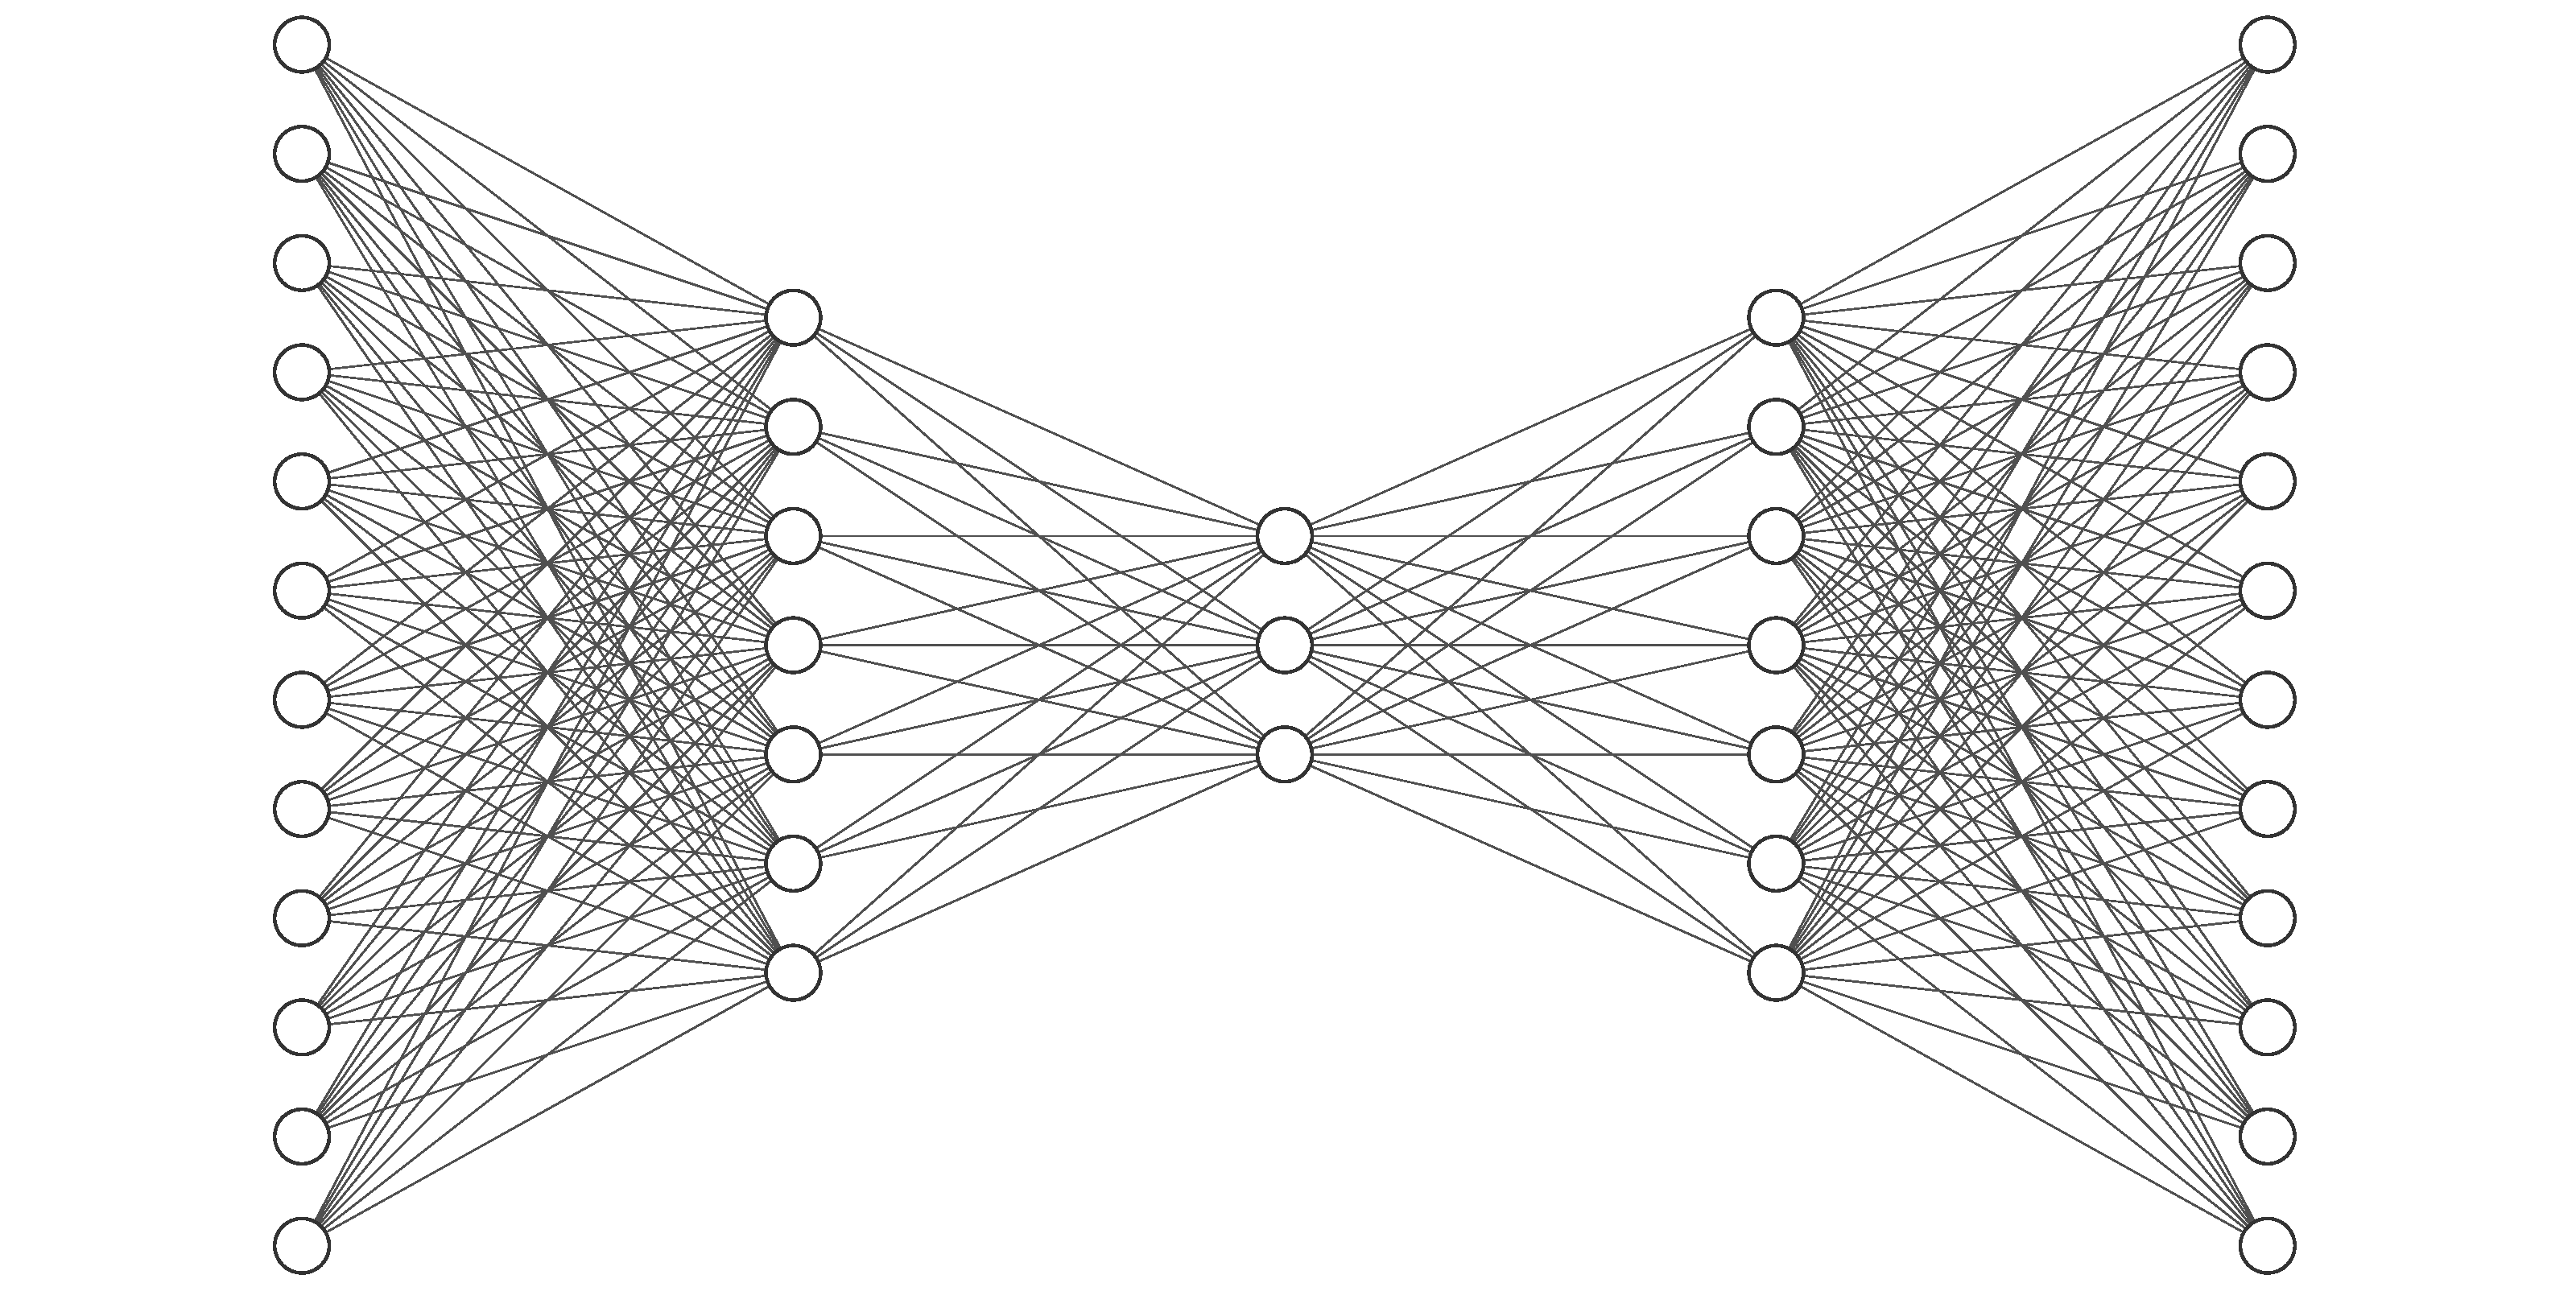
\includegraphics[width=\textwidth]{5_layer_AE.pdf}
		\caption{Autoencoder mit fünf Schichten und dreidimensionalem Bottleneck.}
	\end{center}
\end{figure}

\subsection{Variational Autoencoder}
\label{ch:MethodenDerDimRed:modern:VAE}
\nomenclature[Z]{VAE}{Variational Autoencoder}

\subsection{Self-Organizing Maps}
\label{ch:MethodenDerDimRed:modern:SOM}
\nomenclature[Z]{SOM}{Self-Organizing Map}

%% ==============================
\chapter{Vergleich der Methoden}
\label{ch:Vergleich}
%% ==============================

In \chapref{ch:Dimensionsreduktion} wurden grundlegende Begriffe geklärt und in
\chapref{ch:MethodenDerDimRed} sechs Methoden der Dimensionsreduktion näher betrachtet. Im jetzigen
Kapitel werden die statistischen Methoden aus \secref{ch:MethodenDerDimRed:statistisch} mit den
Machine Learning Methoden aus \secref{ch:MethodenDerDimRed:modern} empirisch auf künstlichen und
natürlichen Datensätzen verglichen. Dazu wird in \secref{ch:Vergleich:sec:Methodik} auf die
Methodik des Vergleichs eingegangen, indem die Schätzung der intrinsischen Dimension und die
eingesetzten Qualitätskriterien erläutert werden. Außerdem werden in
\secref{ch:Vergleich:sec:VerwendeteDatensaetze} die verwendeten Datensätze und in
\secref{ch:Vergleich:sec:ParameterwahlTrainingsdetails} die Parameterwahl der Methoden und
insbesondere die Architektur der Autoencoder vorgestellt. Letztlich werden in
\secref{ch:Vergleich:sec:Resultate} die Resultate des empirischen Vergleichs diskutiert.

\section{Methodik}
\label{ch:Vergleich:sec:Methodik}

Um die statistischen Methoden mit den Machine Learning Ansätzen zu vergleichen, wird die
Performance der Methoden auf mehreren künstlichen sowie natürlichen Datensätzen mit der
Vertrauenswürdigkeit, der Kontinuität und dem $\lcmc$-Kriterium gemessen. Diese Kriterien werden
jeweils für mehrere Nachbarschaftsgrößen berechnet, um eine größere Aussagekraft über die Güte der
gefundenen niedrigdimensionalen Repräsentation zu erreichen. Die Qualitätskriterien werden in
\subsecref{ch:Vergleich:sec:Methodik:subsec:Qualitaetskriterien} eingehend erläutert. Für den
Vergleich werden zwei künstliche und vier natürliche Datensätze verwendet, die in
\secref{ch:Vergleich:sec:VerwendeteDatensaetze} genauer vorgestellt werden. Insgesamt soll damit
ein Überblick über die Stärken und Schwächen der statistischen und der Machine Learning Methoden
geschafft werden. Wie in \subsecref{ch:MethodenDerDimRed:ML:AE:VerhaeltnisPCA} erwähnt, besteht
zwischen Autoencodern und der Hauptkomponentenanalyse eine enge Verbindung. Neben dem Vergleich der
zwei Gruppen wird daher in \secref{ch:Vergleich:sec:Resultate:PCA_AE} der Zusammenhang zwischen der
Hauptkomponentenanalyse und einem linearen Autoencoder genauer untersucht.

\subsection{Qualitätskriterien der Dimensionsreduktion}
\label{ch:Vergleich:sec:Methodik:subsec:Qualitaetskriterien}
Wie bereits in \secref{ch:Dimensionsreduktion} erläutert, hat die Dimensionsreduktion das Ziel einer möglichst \enquote{verlustfreien} Transformation der ursprünglichen Repräsentation in eine latente Repräsentation von geringerer Dimension. Der Rekonstruktionsfehler, den man beispielsweise vom Autoencoder kennt, ist jedoch wie \textcite[18]{vanderMaaten.2009} hervorhebt, nicht sehr aussagekräftig für die Güte einer Dimensionsreduktion. Hinzu kommt, dass der Rekonstruktionsfehler nicht für alle Methoden berechnet werden kann, da eine inverse Transformation der niedrigdimensionalen in die ursprüngliche Repräsentation benötigt wird. Damit fällt der Rekonstruktionsfehler als geeignetes Qualitätskriterium heraus. Das immense Forschungsinteresse für Methoden der Dimensionsreduktion hat daher mit der Zeit dafür gesorgt, dass immer mehr Qualitätskriterien entwickelt wurden. \textcite{Gracia.2014} stellen einige Qualitätskriterien vor und vergleichen diese miteinander. Trotzdem gibt es in der Literatur keine eindeutige Kennzahl, die bei einem Vergleich von Dimensionsreduktionsmethoden standardmäßig eingesetzt wird \parencite[vgl.][1 -- 2]{Lee.2009}. Stattdessen bedient man sich mehrerer Kennzahlen, die
unterschiedliche Dinge bestrafen und versucht so die Stärken und Schwächen einer
Dimensionsreduktionsmethode zu erkennen \parencite[486]{Venna.2001}. Die im Folgenden vorgestellten Qualitätskriterien versuchen die Güte
mithilfe von Rängen zu quantifizieren.

Im ausführlichen Benchmark von \textcite{vanderMaaten.2009} wird auf den Generalisierungsfehler
eines 1-Nächste-Nachbar Klassifikators, sowie auf die zwei Kennzahlen
\newterm{Vertrauenswürdigkeit} (engl. \textit{Trustworthiness}) und \newterm{Kontinuität} (engl.
\textit{Continuity}) \parencites{Venna.2001}{Venna.2006} gesetzt. Die Vertrauenswürdigkeit und die Kontinuität sind
rangbasierte Qualitätskriterien und werden auch in diesem Vergleich eingesetzt. Daneben gibt es
noch viele weitere rangbasierte Qualitätskriterien, welche einheitlich durch die sogenannte
\newterm{Co-Ranking Matrix} \parencite[1432]{Lee.2009} ausgedrückt werden können. Ebenso können die Vertrauenswürdigkeit und
Kontinuität über die Co-Ranking Matrix berechnet werden \parencite[1433]{Lee.2009}. Für eine ausführliche Behandlung dessen wird auf \textcite{Lee.2009}
verwiesen. In dieser Arbeit werden drei Kriterien verwendet: (1) Die Vertrauenswürdigkeit und (2)
die Kontinuität einer Dimensionsreduktion, sowie (3) das \newterm{Local Continuity Meta-Criterion}
(LCMC). Diese werden im Folgenden genauer betrachtet. \nomenclature[Z]{LCMC}{Local Continuity
	Meta-Criterion}

\subsubsection{Vertrauenswürdigkeit und Kontinuität}
\label{ch:Vergleich:sec:Methodik:subsec:Qualitaetskriterien:TC}
Diese beiden Kennzahlen basieren auf der Idee des Erhalts von Nachbarschaften (engl.
\textit{neighborhood preservation}) einer Dimensionsreduktion. Sie bilden also ab, wie gut die
lokale Struktur erhalten wird. Eine $K$-Nachbarschaft $\set{M}_i(K)$ eines Punktes $\vect{x}_i$ ist
definiert als die Menge der Indizes der $K$-nächsten Punkte zu $\vect{x}_i$ ($i = 1, \ldots, n$).
Analog kann die $K$-Nachbarschaft $\widetilde{\set{M}}_i(K)$ des dazugehörigen niedrigdimensionalen
Punktes $\vect{y}_i$ definiert werden. Diese Nachbarschaft wird in einer Dimensionsreduktion
erhalten, wenn $\set{M}_i(K) = \widetilde{\set{M}}_i(K)$, das heißt die Nachbarschaften bleiben von
der Dimensionsreduktion unverändert.

Zum einen kann es nun passieren, dass Punkte, die \textit{vor} der Projektion weit weg voneinander
lagen, \textit{nach} der Projektion aber nah beieinander sind. Mit anderen Worten können Punkte,
die eigentlich unterschiedlich sind, nun ähnlich erscheinen. Aus diesem Grund sagt man, dass die
Vertrauenswürdigkeit der Dimensionsreduktion niedrig ist. Zum anderen ist der gegenteilige Fall
möglich. Nah beieinander liegende Punkte sind nach der Projektion weit weg voneinander. Dies
reduziert die Kontinuität einer Dimensionsreduktion \parencite[486 -- 487]{Venna.2001}.

Formal definiert man zusätzlich zu den Nachbarschaftsmengen von oben die beiden Mengen
$\set{U}_i(K)$ und $\set{V}_i(K)$ wie folgt:
\begin{gather}
	\set{U}_i(K) =  \left\{ j \in \N \mid j \notin \set{M}_i(K) \land j \in \widetilde{\set{M}}_i(K) \right\} \, , \\
	\set{V}_i(K) =  \left\{ j \in \N \mid j \in \set{M}_i(K) \land j \notin \widetilde{\set{M}}_i(K) \right\} \, .
\end{gather}
Diese beiden Mengen bilden lediglich die zwei intuitiv besprochenen Fälle im vorherigen Absatz mathematisch ab. Hierbei entspricht $\set{U}_i(K)$ dem ersten und $\set{V}_i(K)$ dem zweiten Fall.
Damit kann die Vertrauenswürdigkeit $T(K)$ als
\begin{equation}
	T(K) = 1 - \frac{2}{nK(2n - 3K - 1)} \sum_{i = 1}^{n}\sum_{j \in \set{U}_i(K) } \left( r­_{\vect{y}}(i, j) - K \right)
\end{equation}
definiert werden \parencite[487]{Venna.2001}, wobei $r_{\vect{y}}(i, j)$ den Rang von des niedrigdimensionalen Vektors
$\vect{y}_j$ bezeichnet, wenn die Datenpunkte absteigend nach der euklidischen Distanz von
$\vect{y}_i$ geordnet sind. Der Term vor der Summation skaliert das Qualitätskriterium so, dass $0
	\leq T(K) \leq 1$ gilt.\footnote{Dies gilt nur für den Fall, dass $K < n/2$ gilt.} Ein Wert von
$T(K) = 1­$ spricht für eine hohe Vertrauenswürdigkeit.

Analog wird die Kontinuität $C(K)$ über $\set{V}_i(K)$ wie folgt definiert
\begin{equation}
	C(K) = 1 - \frac{2}{nK(2n - 3K - 1)} \sum_{i = 1}^{n}\sum_{j \in \set{V}_i(K) } \left( r_{\vect{x}}(i, j) - K \right) \, ,
\end{equation}
wobei $r_{\vect{x}}(i, j)$ nun den Rang zwischen den Datenpunkten in der hochdimensionalen Repräsentation bezeichnet \parencite[487]{Venna.2001}. Auch hier gilt $0 \leq C(K) \leq 1$ und höher ist besser. Die Kontinuität
misst also, wie gut die ursprünglichen Nachbarschaften erhalten werden.

Üblicherweise werden die beiden Kriterien für mehrere Werte der Nachbarschaftsgröße $K$ berechnet und in einer Abbildung dargestellt. So entfällt die etwas willkürliche Wahl einer spezifischen Nachbarschaftsgröße und ermöglicht die Betrachtung von sowohl sehr kleinen als auch größeren Nachbarschaften.
% \subsubsection{Die Co-Ranking Matrix}
% Ein Eintrag $q_{kl}$ der Co-Ranking Matrix $\mat{Q}$ ist die Anzahl der Paare von Datenpunkten $(i,
% 	j)$, die den Rang $r_{\vect{x}}(i, j) = k$ in der hochdimensionalen und den Rang $r_{\vect{y}}(i,
% 	j) = l$ in der niedrigdimensionalen Repräsentation haben.

\subsubsection{Local Continuity Meta Criterion}
\label{ch:Vergleich:sec:Methodik:subsec:Qualitaetskriterien:LCMC}
\ldots
\subsection{Schätzen der intrinsischen Dimension}
\label{ch:Vergleich:sec:Methodik:subsec:SchaetzenDerIntrinsischenDim}

Bis jetzt wurde immer angenommen, dass die intrinsische Dimension $d$ der Daten bekannt ist, da die
meisten Dimensionsreduktionsmethoden die intrinsische Dimension nicht selbst berechnen. Das
Schätzen der intrinsischen Dimension ist also ein nicht unwichtiges Teilproblem der
Dimensionsreduktion, da eine Unterschätzung von $d$ dazu führt, dass relevante Strukturen
zwangsweise verloren gehen \parencite[1]{Levina.2004}. Erschwert wird dieses Problem durch die Tatsache, dass es sehr viele
Definitionen der intrinsischen Dimension und damit auch sehr viele unterschiedliche Schätzer gibt.
Im Folgenden soll ein kurzer Überblick verschafft werden, jedoch geht eine detaillierte Behandlung
der Schätzung über den Rahmen dieser Arbeit hinaus. Daher wird für einen Überblick und Vergleich
dieser Schätzer auf \textcites{Campadelli.2015}{Bac.2021}{Verveer.1995} verwiesen.

In \secref{ch:Dimensionsreduktion:MannigfaltigkeitenIntrinsDim} haben wir die \textit{topologische
	Dimension} kennengelernt, welche sich in der Literatur zur Strukturerkennung durchgesetzt hat \parencite[1]{Campadelli.2015}. Allerdings bringt diese Definition praktische Schwierigkeiten mit sich,
weswegen die meisten Schätzer der intrinsischen Dimension auf der damit verwandten
\textit{fraktalen Dimension} wie zum Beispiel der Schätzer der Korrelationsdimension \parencite{Camastra.2002} basieren. Daneben gibt es noch Nächste-Nachbar-basierte Schätzer \parencite[1]{Campadelli.2015}. Zu dieser Kategorie gehört auch der weit verbreitete und in dieser
Arbeit verwendete \newterm{Maximum Likelihood Schätzer} von \textcite{Levina.2004}. Diese Schätzer
betrachten die Verteilung der Nachbarschaft eines Punktes $\rvect{x}$ als Funktion der
intrinsischen Dimension -- üblicherweise innerhalb einer kleinen Kugel um $\rvect{x}$
\parencite[8]{Campadelli.2015}. Der Maximum Likelihood Schätzer nimmt an, dass die Beobachtungen, die
in einer solchen Kugel liegen, einem homogenen Poisson-(Zähl-)Prozess folgen
\parencite[2]{Levina.2004}. Dieser Prozess hängt von $d$ ab, weshalb mittels der Maximum Likelihood
Methode ein Schätzwert $\estNormal{d}$ für einen fixen Punkt $\rvect{x}_i$ als
\begin{equation}
	\estNormal{d}_K(\vect{x}_i) = \left( \frac{1}{K - 1} \sum_{j=1}^{K - 1} \log \frac{T_K(\vect{x}_i)}{T_j(\vect{x}_i)} \right)^{-1}
\end{equation}
berechnet werden kann \parencite[4]{Levina.2004}. Hierbei ist $K$ die Anzahl der nächste Nachbarn und $T_{K}(\vect{x}_i)$ die
euklidische Distanz von $\vect{x}_i$ zu seinem $K$-ten Nachbar. Dies ist jedoch nur eine lokale
Schätzung für einen fixen Punkt $\vect{x}_i$. Um eine globale Schätzung zu erhalten, wird der
Mittelwert über alle Beobachtungen für mehrere Werte von $K$ gebildet.
\section{Verwendete Datensätze}
\label{ch:Vergleich:sec:VerwendeteDatensaetze}
Es werden sowohl künstliche als auch natürliche Datensätze eingesetzt, um Eigenschaften der
verschiedenen Methoden miteinander zu vergleichen. Eine Übersicht über die Dimensionen und Stichprobengrößen der verwendeten Datensätze befindet sich in Tabelle \ref{tab:uebersicht-datensaetze}.

\subsection{Künstliche Datensätze}
\label{ch:Vergleich:sec:VerwendeteDatensaetze:kuenstlich}
Zu den künstlichen Datensätzen gehört die weitverbreitete \textit{Swiss Roll} und der \textit{Twin Peaks} Datensatz,
\begin{figure}[ht]
	\begin{center}
		\input{\figures/artificial_datasets.pgf}
	\end{center}
	\caption[Künstliche Datensätze]{\figleft Die Swiss Roll. Die intrinsische Dimension beträgt zwei weil die Daten auf einer \enquote{eingerollten Ebene} liegen. Die Dimensionsreduktionsmethoden müssen die Swiss Roll \enquote{entfalten}, um eine zweidimensionale Repräsentation zu erhalten. \figright Der Twin Peaks Datensatz. Dieser besteht aus je zwei spitzen Bergen, die nach oben und unten zeigen. Auch dieser Datensatz hat eine intrinsische Dimension von zwei, denn die Berge können \enquote{plattgedrückt} werden, womit man eine zweidimensionale Repräsentation erhält.}
	\label{fig:ArtificialDatasets}
\end{figure}
die in \figref{fig:ArtificialDatasets} dargestellt sind.
Beide künstlichen Datensätze bestehen aus 5000 Datenpunkten und haben eine extrinsische Dimension von drei und eine intrinsische
Dimension von zwei. Dies erlaubt eine visuelle Betrachtung der Datensätze und der gefundenen
latenten Räume, schränkt aber gleichzeitig die Architektur eines (unterbestimmten) Autoencoders
sehr ein. Künstliche Datensätze sind aber nicht zwangsweise aussagekräftig für die Performance auf echten Datensätzen, weswegen zusätzlich vier natürliche Datensätze hinzugezogen werden.

\subsection{Natürliche Datensätze}
\label{ch:Vergleich:sec:VerwendeteDatensaetze:natuerlich}
Natürliche
Datensätze weisen empirischen Ergebnissen zufolge \addref oft komplexe nichtlineare Zusammenhänge
auf und sind daher für die Dimensionsreduktion anspruchsvoller als kleine, künstlich generierte
Datensätze. Der Nachteil besteht darin, dass die intrinsische Dimension in der Regel deutlich über
zwei liegt und daher der latente Raum nicht visualisiert werden kann. Nichtsdestotrotz liefern die
Qualitätskriterien hinreichende gute Indizien für die Performance der Methoden. Bei den natürlichen
Datensätzen wurden größtenteils Bilddatensätze, aber auch ein Textdatensatz ausgewählt, da diese eine
sehr hohe extrinsische Dimension aufweisen und daher für die Dimensionsreduktion gut geeignet sind.
Konkret wurde (1) der \textit{MNIST}-Datensatz \parencite{LeCun.2010}, (2) der \textit{Olivetti Face}-Datensatz
\footnote{\url{https://cam-orl.co.uk/facedatabase.html}}, (3) der \textit{Labeled Faces in the
	Wild} (LFW) Datensatz \parencite{GaryB.Huang.2007}, (4) der \textit{Facial Emotion Recognition} (FER) Datensatz \parencite{DumitruIanGoodfellowWillCukierskiYoshuaBengio.2013} und (5) der \textit{ICMR}-Datensatz
ausgewählt, um die Performance der Dimensionsreduktionsmethoden auf natürlichen Datensätzen zu
evaluieren. Der weit verbreitete MNIST-Datensatz besteht aus 60 000 Grauton-Bildern von
handgeschriebenen Zahlen in der Auflösung $28 \times 28$. Die Anzahl der Pixel und damit die
extrinsische Dimension beträgt 784. Der \textit{Olivetti Face}-Datensatz enthält Bilder von
Gesichtern aus zehn unterschiedlichen Positionen von 40 Personen und ist damit der kleinste
natürliche Datensatz in diesem Vergleich mit 400 Bildern. Die Bilder haben eine Auflösung von $64
	\times 64$, was einer extrinsischen Dimension von 4096 entspricht. Der LFW-Datensatz enthält
insgesamt über 13 000 Bilder von Gesichtern, jedoch wurde hier eine Teilmenge ausgewählt, sodass
jede Person mindestens 30 mal vorkommt. Dies resultiert in einer Stichprobengröße von 2370. Die
Bilder haben eine Auflösung von $62 \times 47$ und damit eine extrinsische Dimension von 2914. Der
FER Datensatz besteht aus 28 709 Bildern von Gesichtern mit sechs unterschiedlichen Emotionen. Die
Bilder haben eine Auflösung von $48 \times 48$ und sind damit 2304-dimensional. Beispiele der
Bild-Datensätze sind in \figref{fig:Dataset_samples} zu finden.
\begin{figure}
	\begin{center}
		%% Creator: Matplotlib, PGF backend
%%
%% To include the figure in your LaTeX document, write
%%   \input{<filename>.pgf}
%%
%% Make sure the required packages are loaded in your preamble
%%   \usepackage{pgf}
%%
%% Also ensure that all the required font packages are loaded; for instance,
%% the lmodern package is sometimes necessary when using math font.
%%   \usepackage{lmodern}
%%
%% Figures using additional raster images can only be included by \input if
%% they are in the same directory as the main LaTeX file. For loading figures
%% from other directories you can use the `import` package
%%   \usepackage{import}
%%
%% and then include the figures with
%%   \import{<path to file>}{<filename>.pgf}
%%
%% Matplotlib used the following preamble
%%   
%%   \usepackage{fontspec}
%%   \setmainfont{DejaVuSerif.ttf}[Path=\detokenize{/Users/moritzmistol/.pyenv/versions/3.9.13/envs/thesis/lib/python3.9/site-packages/matplotlib/mpl-data/fonts/ttf/}]
%%   \setsansfont{DejaVuSans.ttf}[Path=\detokenize{/Users/moritzmistol/.pyenv/versions/3.9.13/envs/thesis/lib/python3.9/site-packages/matplotlib/mpl-data/fonts/ttf/}]
%%   \setmonofont{DejaVuSansMono.ttf}[Path=\detokenize{/Users/moritzmistol/.pyenv/versions/3.9.13/envs/thesis/lib/python3.9/site-packages/matplotlib/mpl-data/fonts/ttf/}]
%%   \makeatletter\@ifpackageloaded{underscore}{}{\usepackage[strings]{underscore}}\makeatother
%%
\begingroup%
\makeatletter%
\begin{pgfpicture}%
\pgfpathrectangle{\pgfpointorigin}{\pgfqpoint{5.850000in}{6.860552in}}%
\pgfusepath{use as bounding box, clip}%
\begin{pgfscope}%
\pgfsetbuttcap%
\pgfsetmiterjoin%
\definecolor{currentfill}{rgb}{1.000000,1.000000,1.000000}%
\pgfsetfillcolor{currentfill}%
\pgfsetlinewidth{0.000000pt}%
\definecolor{currentstroke}{rgb}{1.000000,1.000000,1.000000}%
\pgfsetstrokecolor{currentstroke}%
\pgfsetdash{}{0pt}%
\pgfpathmoveto{\pgfqpoint{0.000000in}{0.000000in}}%
\pgfpathlineto{\pgfqpoint{5.850000in}{0.000000in}}%
\pgfpathlineto{\pgfqpoint{5.850000in}{6.860552in}}%
\pgfpathlineto{\pgfqpoint{0.000000in}{6.860552in}}%
\pgfpathlineto{\pgfqpoint{0.000000in}{0.000000in}}%
\pgfpathclose%
\pgfusepath{fill}%
\end{pgfscope}%
\begin{pgfscope}%
\pgfsetbuttcap%
\pgfsetmiterjoin%
\definecolor{currentfill}{rgb}{1.000000,1.000000,1.000000}%
\pgfsetfillcolor{currentfill}%
\pgfsetlinewidth{0.000000pt}%
\definecolor{currentstroke}{rgb}{1.000000,1.000000,1.000000}%
\pgfsetstrokecolor{currentstroke}%
\pgfsetdash{}{0pt}%
\pgfpathmoveto{\pgfqpoint{-0.025000in}{3.508890in}}%
\pgfpathlineto{\pgfqpoint{2.925000in}{3.508890in}}%
\pgfpathlineto{\pgfqpoint{2.925000in}{7.008890in}}%
\pgfpathlineto{\pgfqpoint{-0.025000in}{7.008890in}}%
\pgfpathlineto{\pgfqpoint{-0.025000in}{3.508890in}}%
\pgfpathclose%
\pgfusepath{fill}%
\end{pgfscope}%
\begin{pgfscope}%
\pgfpathrectangle{\pgfqpoint{0.050000in}{5.477218in}}{\pgfqpoint{1.333333in}{1.333333in}}%
\pgfusepath{clip}%
\pgfsys@transformshift{0.050000in}{5.477218in}%
\pgftext[left,bottom]{
\includegraphics[interpolate=true,width=1.340000in,height=1.340000in]{dataset_samples-img0.png}}%
\end{pgfscope}%
\begin{pgfscope}%
\pgfpathrectangle{\pgfqpoint{1.516667in}{5.477218in}}{\pgfqpoint{1.333333in}{1.333333in}}%
\pgfusepath{clip}%
\pgfsys@transformshift{1.516667in}{5.477218in}%
\pgftext[left,bottom]{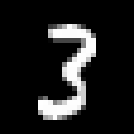
\includegraphics[interpolate=true,width=1.340000in,height=1.340000in]{dataset_samples-img1.png}}%
\end{pgfscope}%
\begin{pgfscope}%
\pgfpathrectangle{\pgfqpoint{0.050000in}{3.982228in}}{\pgfqpoint{1.333333in}{1.333333in}}%
\pgfusepath{clip}%
\pgfsys@transformshift{0.050000in}{3.982228in}%
\pgftext[left,bottom]{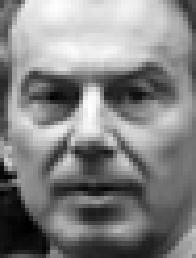
\includegraphics[interpolate=true,width=1.340000in,height=1.340000in]{dataset_samples-img2.png}}%
\end{pgfscope}%
\begin{pgfscope}%
\pgfpathrectangle{\pgfqpoint{1.516667in}{3.982228in}}{\pgfqpoint{1.333333in}{1.333333in}}%
\pgfusepath{clip}%
\pgfsys@transformshift{1.516667in}{3.982228in}%
\pgftext[left,bottom]{
\includegraphics[interpolate=true,width=1.340000in,height=1.340000in]{dataset_samples-img3.png}}%
\end{pgfscope}%
\begin{pgfscope}%
\definecolor{textcolor}{rgb}{0.000000,0.000000,0.000000}%
\pgfsetstrokecolor{textcolor}%
\pgfsetfillcolor{textcolor}%
\pgftext[x=1.509000in,y=3.683890in,,base]{\color{textcolor}\rmfamily\fontsize{10.000000}{12.000000}\selectfont (a)}%
\end{pgfscope}%
\begin{pgfscope}%
\pgfsetbuttcap%
\pgfsetmiterjoin%
\definecolor{currentfill}{rgb}{1.000000,1.000000,1.000000}%
\pgfsetfillcolor{currentfill}%
\pgfsetlinewidth{0.000000pt}%
\definecolor{currentstroke}{rgb}{1.000000,1.000000,1.000000}%
\pgfsetstrokecolor{currentstroke}%
\pgfsetdash{}{0pt}%
\pgfpathmoveto{\pgfqpoint{-0.025000in}{0.008890in}}%
\pgfpathlineto{\pgfqpoint{2.925000in}{0.008890in}}%
\pgfpathlineto{\pgfqpoint{2.925000in}{3.508890in}}%
\pgfpathlineto{\pgfqpoint{-0.025000in}{3.508890in}}%
\pgfpathlineto{\pgfqpoint{-0.025000in}{0.008890in}}%
\pgfpathclose%
\pgfusepath{fill}%
\end{pgfscope}%
\begin{pgfscope}%
\pgfpathrectangle{\pgfqpoint{0.117792in}{1.853880in}}{\pgfqpoint{1.197749in}{1.580009in}}%
\pgfusepath{clip}%
\pgfsys@transformshift{0.117792in}{1.853880in}%
\pgftext[left,bottom]{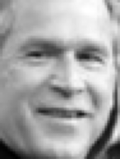
\includegraphics[interpolate=true,width=1.200000in,height=1.590000in]{dataset_samples-img4.png}}%
\end{pgfscope}%
\begin{pgfscope}%
\pgfpathrectangle{\pgfqpoint{1.584459in}{1.853880in}}{\pgfqpoint{1.197749in}{1.580009in}}%
\pgfusepath{clip}%
\pgfsys@transformshift{1.584459in}{1.853880in}%
\pgftext[left,bottom]{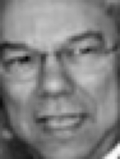
\includegraphics[interpolate=true,width=1.200000in,height=1.590000in]{dataset_samples-img5.png}}%
\end{pgfscope}%
\begin{pgfscope}%
\pgfpathrectangle{\pgfqpoint{0.117792in}{0.358890in}}{\pgfqpoint{1.197749in}{1.580009in}}%
\pgfusepath{clip}%
\pgfsys@transformshift{0.117792in}{0.358890in}%
\pgftext[left,bottom]{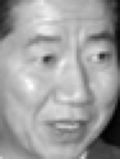
\includegraphics[interpolate=true,width=1.200000in,height=1.590000in]{dataset_samples-img6.png}}%
\end{pgfscope}%
\begin{pgfscope}%
\pgfpathrectangle{\pgfqpoint{1.584459in}{0.358890in}}{\pgfqpoint{1.197749in}{1.580009in}}%
\pgfusepath{clip}%
\pgfsys@transformshift{1.584459in}{0.358890in}%
\pgftext[left,bottom]{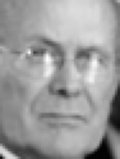
\includegraphics[interpolate=true,width=1.200000in,height=1.590000in]{dataset_samples-img7.png}}%
\end{pgfscope}%
\begin{pgfscope}%
\definecolor{textcolor}{rgb}{0.000000,0.000000,0.000000}%
\pgfsetstrokecolor{textcolor}%
\pgfsetfillcolor{textcolor}%
\pgftext[x=1.509000in,y=0.078890in,,base]{\color{textcolor}\rmfamily\fontsize{10.000000}{12.000000}\selectfont (c)}%
\end{pgfscope}%
\begin{pgfscope}%
\pgfsetbuttcap%
\pgfsetmiterjoin%
\definecolor{currentfill}{rgb}{1.000000,1.000000,1.000000}%
\pgfsetfillcolor{currentfill}%
\pgfsetlinewidth{0.000000pt}%
\definecolor{currentstroke}{rgb}{1.000000,1.000000,1.000000}%
\pgfsetstrokecolor{currentstroke}%
\pgfsetdash{}{0pt}%
\pgfpathmoveto{\pgfqpoint{2.925000in}{3.508890in}}%
\pgfpathlineto{\pgfqpoint{5.875000in}{3.508890in}}%
\pgfpathlineto{\pgfqpoint{5.875000in}{7.008890in}}%
\pgfpathlineto{\pgfqpoint{2.925000in}{7.008890in}}%
\pgfpathlineto{\pgfqpoint{2.925000in}{3.508890in}}%
\pgfpathclose%
\pgfusepath{fill}%
\end{pgfscope}%
\begin{pgfscope}%
\pgfpathrectangle{\pgfqpoint{3.000000in}{5.477218in}}{\pgfqpoint{1.333333in}{1.333333in}}%
\pgfusepath{clip}%
\pgfsys@transformshift{3.000000in}{5.477218in}%
\pgftext[left,bottom]{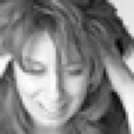
\includegraphics[interpolate=true,width=1.340000in,height=1.340000in]{dataset_samples-img8.png}}%
\end{pgfscope}%
\begin{pgfscope}%
\pgfpathrectangle{\pgfqpoint{4.466667in}{5.477218in}}{\pgfqpoint{1.333333in}{1.333333in}}%
\pgfusepath{clip}%
\pgfsys@transformshift{4.466667in}{5.477218in}%
\pgftext[left,bottom]{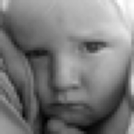
\includegraphics[interpolate=true,width=1.340000in,height=1.340000in]{dataset_samples-img9.png}}%
\end{pgfscope}%
\begin{pgfscope}%
\pgfpathrectangle{\pgfqpoint{3.000000in}{3.982228in}}{\pgfqpoint{1.333333in}{1.333333in}}%
\pgfusepath{clip}%
\pgfsys@transformshift{3.000000in}{3.982228in}%
\pgftext[left,bottom]{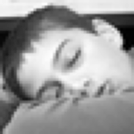
\includegraphics[interpolate=true,width=1.340000in,height=1.340000in]{dataset_samples-img10.png}}%
\end{pgfscope}%
\begin{pgfscope}%
\pgfpathrectangle{\pgfqpoint{4.466667in}{3.982228in}}{\pgfqpoint{1.333333in}{1.333333in}}%
\pgfusepath{clip}%
\pgfsys@transformshift{4.466667in}{3.982228in}%
\pgftext[left,bottom]{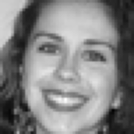
\includegraphics[interpolate=true,width=1.340000in,height=1.340000in]{dataset_samples-img11.png}}%
\end{pgfscope}%
\begin{pgfscope}%
\definecolor{textcolor}{rgb}{0.000000,0.000000,0.000000}%
\pgfsetstrokecolor{textcolor}%
\pgfsetfillcolor{textcolor}%
\pgftext[x=4.459000in,y=3.683890in,,base]{\color{textcolor}\rmfamily\fontsize{10.000000}{12.000000}\selectfont (b)}%
\end{pgfscope}%
\begin{pgfscope}%
\pgfsetbuttcap%
\pgfsetmiterjoin%
\definecolor{currentfill}{rgb}{1.000000,1.000000,1.000000}%
\pgfsetfillcolor{currentfill}%
\pgfsetlinewidth{0.000000pt}%
\definecolor{currentstroke}{rgb}{1.000000,1.000000,1.000000}%
\pgfsetstrokecolor{currentstroke}%
\pgfsetdash{}{0pt}%
\pgfpathmoveto{\pgfqpoint{2.925000in}{0.008890in}}%
\pgfpathlineto{\pgfqpoint{5.875000in}{0.008890in}}%
\pgfpathlineto{\pgfqpoint{5.875000in}{3.508890in}}%
\pgfpathlineto{\pgfqpoint{2.925000in}{3.508890in}}%
\pgfpathlineto{\pgfqpoint{2.925000in}{0.008890in}}%
\pgfpathclose%
\pgfusepath{fill}%
\end{pgfscope}%
\begin{pgfscope}%
\pgfpathrectangle{\pgfqpoint{3.000000in}{1.977218in}}{\pgfqpoint{1.333333in}{1.333333in}}%
\pgfusepath{clip}%
\pgfsys@transformshift{3.000000in}{1.977218in}%
\pgftext[left,bottom]{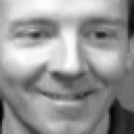
\includegraphics[interpolate=true,width=1.340000in,height=1.340000in]{dataset_samples-img12.png}}%
\end{pgfscope}%
\begin{pgfscope}%
\pgfpathrectangle{\pgfqpoint{4.466667in}{1.977218in}}{\pgfqpoint{1.333333in}{1.333333in}}%
\pgfusepath{clip}%
\pgfsys@transformshift{4.466667in}{1.977218in}%
\pgftext[left,bottom]{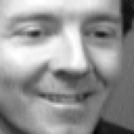
\includegraphics[interpolate=true,width=1.340000in,height=1.340000in]{dataset_samples-img13.png}}%
\end{pgfscope}%
\begin{pgfscope}%
\pgfpathrectangle{\pgfqpoint{3.000000in}{0.482228in}}{\pgfqpoint{1.333333in}{1.333333in}}%
\pgfusepath{clip}%
\pgfsys@transformshift{3.000000in}{0.482228in}%
\pgftext[left,bottom]{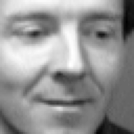
\includegraphics[interpolate=true,width=1.340000in,height=1.340000in]{dataset_samples-img14.png}}%
\end{pgfscope}%
\begin{pgfscope}%
\pgfpathrectangle{\pgfqpoint{4.466667in}{0.482228in}}{\pgfqpoint{1.333333in}{1.333333in}}%
\pgfusepath{clip}%
\pgfsys@transformshift{4.466667in}{0.482228in}%
\pgftext[left,bottom]{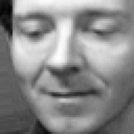
\includegraphics[interpolate=true,width=1.340000in,height=1.340000in]{dataset_samples-img15.png}}%
\end{pgfscope}%
\begin{pgfscope}%
\definecolor{textcolor}{rgb}{0.000000,0.000000,0.000000}%
\pgfsetstrokecolor{textcolor}%
\pgfsetfillcolor{textcolor}%
\pgftext[x=4.459000in,y=0.078890in,,base]{\color{textcolor}\rmfamily\fontsize{10.000000}{12.000000}\selectfont (d)}%
\end{pgfscope}%
\end{pgfpicture}%
\makeatother%
\endgroup%

	\end{center}
	\caption{Beispielbilder der natürlichen Datensätze}
	\label{fig:Dataset_samples}
\end{figure}

Letztlich ist der
ICMR-Datensatz\footnote{\url{https://www.kaggle.com/datasets/shibumohapatra/icmr-data?select=labels.csv}}
enthält die Genausprägungen von 801 Personen, die mit fünf unterschiedlichen Arten von Krebs
diagnostiziert wurden. Der Datensatz enthält Genausprägungen von über 20 000 Genen, womit dieser
Datensatz die höchste extrinsische Dimension im Vergleich besitzt. In Tabelle
\ref{tab:uebersicht-datensaetze} sind die extrinsischen und intrinsischen Dimensionen, sowie die
Stichprobengröße der Datensätze zusammengefasst. Die intrinsischen Dimensionen sind die Schätzungen
des in \subsecref{ch:Vergleich:sec:Methodik:subsec:SchaetzenDerIntrinsischenDim} erläuterten
Maximum Likelihood Schätzers für den jeweiligen Datensatz.

\begin{table}[]
	\centering
	\begin{tabular}{@{}cccc@{}}
		\toprule
		Datensatz      & extrinsische Dimension $D$ & intrinsische Dimension $d$ & Stichprobengröße $n$ \\ \midrule
		Swiss Roll     & 3                          & 2                          & 5000                 \\
		Twin Peaks     & 3                          & 2                          & 5000                 \\
		MNIST          & 784                        & 10                         & 60 000               \\
		Olivetti Faces & 4096                       & 10                         & 400                  \\
		LFW            & 2914                       & 21                         & 2370                 \\
		FER            & 2304                       & 26 (6)                     & 28 709               \\
		ICMR           & 20 531                     & 22                         & 801                  \\
		\bottomrule
	\end{tabular}
	\caption{Übersicht über die extrinsischen und intrinsischen Dimensionen, sowie die Stichprobengröße der in diesem Vergleich verwendeten Datensätze. Bei Bilddatensätzen entspricht die extrinsische Dimension der Anzahl der Pixel im Bild.}
	\label{tab:uebersicht-datensaetze}
\end{table}

\section{Parameterwahl und Trainingsdetails}
\label{ch:Vergleich:sec:ParameterwahlTrainingsdetails}

In diesem Abschnitt werden die gewählten (Hyper-)Parameter und Details des Trainierens der
Dimensionsreduktionsmethoden vorgestellt. Eine Übersicht ist in Tabelle xxx zu finden. Für die
Hauptkomponentenanalyse gibt es neben der Anzahl der zu behaltenden Hauptkomponenten keine
Parameter. Die Anzahl der Hauptkomponenten entspricht der intrinsischen Dimension, welche vom
Datensatz abhängt und für alle Methoden identisch ist. Dies trifft analog auf Kernel PCA und auf
Locally Linear Embedding zu. Für Autoencoder bestimmt die intrinsische Dimension die Größe der
Bottleneck-Schicht. Für Kernel PCA wird ein RBF-Kernel (Gauß-Kernel) eingesetzt, wofür ein
Hyperparameter $\gamma$ gewählt werden kann. Dieser wird Datensatz-spezifisch auf $\gamma =
	\sfrac{1}{D}$ gesetzt. Für Locally Linear Embedding gibt es mehrere Parameter: (1) einen Parameter
$K$, der die Größe der verwendeten Nachbarschaft kontrolliert und (2) eine
Regularisierungs-Konstante $\epsilon$, die auf die Diagonale der lokalen Kovarianzmatrix addiert
wird.

Den statistischen Methoden gegenüber haben Autoencoder deutlich mehr Freiheitsgrade, um die
Architektur zu bestimmen. Die wichtigsten Parameter sind die Anzahl der Schichten $m$, sowie die
Anzahl an Neuronen pro Schicht und die Wahl der Aktivierungsfunktionen. Daneben gibt es noch viele
weitere Freiheitsgrade für das Trainieren des Autoencoders, welche teilweise vom Datensatz
abhängen. Diese wurden für alle Autoencoder nahezu identisch gewählt und werden in
Appendix~\ref{ch:Appendix:Architektur-Details} genauer erläutert. Für beide künstlichen Datensätze
und für den Olivetti Face Datensatz wird ein dreischichtiger Autoencoder eingesetzt. Für alle
anderen Datensätze wird ein fünfschichtiger Autoencoder trainiert. Alle vollvernetzten Autoencoder
und der Contractive Autoencoder verwenden Sigmoid-Aktivierungsfunktionen im Encoder und Decoder.
Auf Bilddatensätzen wurden zusätzlich Convolutional Autoencoder trainiert, deren Architekturen an
\textcite[14]{Ghosh.2019} angelehnt sind und ebenfalls in
Appendix~\ref{ch:Appendix:Architektur-Details} spezifiziert sind.

\begin{table}[ht]
	\tymax=300pt
	\centering
	\begin{tabulary}{\linewidth}{@{}CC@{}}
		\toprule
		Methode                            & Parameter                                                            \\ \midrule
		Hauptkomponentenanalyse (PCA)      & --                                                                   \\ \midrule
		Kernel PCA                         & $\kappa(\vect{x}_1, \vect{x}_2) = \exp(- \norm{\vect{x}_1 - \vect{x}_2}^2/(2\gamma^2))$, $\gamma=\sfrac{1}{D}$ \\ \midrule
		Locally Linear Embedding (LLE)     & $K=10$, $\epsilon=1\mathrm{e}{-3}$                                   \\ \midrule
		Autoencoder (AE)                   & $m \in \{3, 5\}$, Sigmoid-Aktivierungsfunktion (siehe
		Appendix~\ref{ch:Appendix:Architektur-Details})                                                           \\ \midrule Contractive Autoencoder (CAE) & $m = 3$, $\lambda=1\mathrm{e}{-4}$,
		Sigmoid-Aktivierungsfunktion (siehe Appendix~\ref{ch:Appendix:Architektur-Details})                       \\ \midrule
		Convolutional Autoencoder (ConvAE) & $m > 5$, ReLU-Aktivierungsfunktion (siehe
		Appendix~\ref{ch:Appendix:Architektur-Details})                                                           \\ \bottomrule
	\end{tabulary}
	\caption[Übersicht über die verwendeten Parameter der Methoden]{Übersicht über die verwendeten Parameter. Hierbei ist $\kappa$ die Kernel-Funktion, $D$ die extrinsische Dimension des Datensatzes, $K$ die Nachbarschaftsgröße, $\epsilon$ eine Regularisierungskonstante für LLE und $m$ die Anzahl der Schichten im Autoencoder.}
	\label{tab:uebersicht-parameter}
\end{table}
\section{Resultate}
\label{ch:Vergleich:sec:Resultate}

In diesem Abschnitt werden die Resultate des empirischen Vergleichs vorgestellt. Dazu werden die
Werte der verschiedenen Qualitätskriterien auf den künstlichen und natürlichen Datensätzen in
Abhängigkeit der Nachbarschaftsgröße $K$ abgebildet. Die verschiedenen Methoden wurden mit den im
vorhergehenden Abschnitt (\secref{ch:Vergleich:sec:ParameterwahlTrainingsdetails}) erläuterten
Parametern auf den künstlichen und natürlichen Datensätzen trainiert und hinsichtlich der in
\secref{ch:Vergleich:sec:Methodik:subsec:Qualitaetskriterien} vorgestellten Qualitätskriterien für
eine Nachbarschaftsgröße von $1 \leq K \leq 100$ evaluiert. Einige der Abbildungen für die
Qualitätskriterien sind im Appendix \ref{ch:Appendix:Qualitaetskriterien} zu finden.\unsure{vlt
	eine Tabelle mit Werten für K=10 (?) einfügen für die Übersicht?} In
\secref{ch:Vergleich:sec:Resultate:kuenstlich} werden die Ergebnisse auf den künstlichen
Datensätzen und in \secref{ch:Vergleich:sec:Resultate:natuerlich} die Ergebnisse auf den
natürlichen Datensätzen diskutiert. Letztlich wird in \secref{ch:Vergleich:sec:Resultate:PCA_AE}
der Zusammenhang zwischen der Hauptkomponentenanalyse und linearen Autoencodern empirisch
untersucht.

\subsection{Resultate auf künstlichen Datensätzen}
\label{ch:Vergleich:sec:Resultate:kuenstlich}

Die Qualitätskriterien für den Swiss Roll Datensatz sind in \figref{fig:SwissRollMetrics}
\begin{figure}[ht]
	\begin{center}
		\input{\figures/SwissRoll_comparison copy.pgf}
	\end{center}
	\caption[Swiss Roll Qualitätskriterien]{Die Vertrauenswürdigkeit und Kontinuität der Dimensionsreduktion, sowie das Local Continuity Meta-Criterion (LCMC) für den Swiss Roll Datensatz. Locally Linear Embedding (LLE) schneidet mit Abstand am besten ab, dicht gefolgt vom Autoencoder (AE) und der Kernel PCA. Die restlichen Methoden unterscheiden sich nicht stark, lediglich bei der Vertrauenswürdigkeit kann sich die Kernel PCA etwas nach oben absetzen. Die PCA und der Autoencoder sind hinsichtlich der Kontinuität und des LCMC sehr ähnlich. (Eigene Darstellung)}
	\label{fig:SwissRollMetrics}
\end{figure}
und die Qualitaetskriterien für den Twin Peaks Datensatz in \figref{fig:TwinPeaksMetrics} abgebildet. Wie dort zu erkennen ist, zeigt Locally Linear Embedding eine sehr starke Performance auf den beiden künstlichen Datensätzen. Der Autoencoder kann sich hinsichtlich des Twin Peaks Datensatzes von den restlichen Methoden abheben. Bei der Swiss Roll ist dies jedoch nicht der Fall. Hier sind die PCA, die Kernel PCA, sowie beide Varianten des Autoencoders relativ ähnlich.

\subsection{Resultate auf natürlichen Datensätzen}
\label{ch:Vergleich:sec:Resultate:natuerlich}

Die Qualitätskriterien auf den natürlichen Datensätzen zeigen ein etwas anderes Bild, als es bei
den künstlichen Datensätzen der Fall war. Die starke Performance von Locally Linear Embedding setzt
sich nicht auf den natürlichen hochdimensionalen Datensätzen fort.
\begin{figure}[ht]
	\begin{center}
		%% Creator: Matplotlib, PGF backend
%%
%% To include the figure in your LaTeX document, write
%%   \input{<filename>.pgf}
%%
%% Make sure the required packages are loaded in your preamble
%%   \usepackage{pgf}
%%
%% Also ensure that all the required font packages are loaded; for instance,
%% the lmodern package is sometimes necessary when using math font.
%%   \usepackage{lmodern}
%%
%% Figures using additional raster images can only be included by \input if
%% they are in the same directory as the main LaTeX file. For loading figures
%% from other directories you can use the `import` package
%%   \usepackage{import}
%%
%% and then include the figures with
%%   \import{<path to file>}{<filename>.pgf}
%%
%% Matplotlib used the following preamble
%%   
%%   \usepackage{fontspec}
%%   \setmainfont{DejaVuSerif.ttf}[Path=\detokenize{/Users/moritzmistol/.pyenv/versions/3.9.13/envs/thesis/lib/python3.9/site-packages/matplotlib/mpl-data/fonts/ttf/}]
%%   \setsansfont{DejaVuSans.ttf}[Path=\detokenize{/Users/moritzmistol/.pyenv/versions/3.9.13/envs/thesis/lib/python3.9/site-packages/matplotlib/mpl-data/fonts/ttf/}]
%%   \setmonofont{DejaVuSansMono.ttf}[Path=\detokenize{/Users/moritzmistol/.pyenv/versions/3.9.13/envs/thesis/lib/python3.9/site-packages/matplotlib/mpl-data/fonts/ttf/}]
%%   \makeatletter\@ifpackageloaded{underscore}{}{\usepackage[strings]{underscore}}\makeatother
%%
\begingroup%
\makeatletter%
\begin{pgfpicture}%
\pgfpathrectangle{\pgfpointorigin}{\pgfqpoint{5.711441in}{4.634154in}}%
\pgfusepath{use as bounding box, clip}%
\begin{pgfscope}%
\pgfsetbuttcap%
\pgfsetmiterjoin%
\definecolor{currentfill}{rgb}{1.000000,1.000000,1.000000}%
\pgfsetfillcolor{currentfill}%
\pgfsetlinewidth{0.000000pt}%
\definecolor{currentstroke}{rgb}{1.000000,1.000000,1.000000}%
\pgfsetstrokecolor{currentstroke}%
\pgfsetdash{}{0pt}%
\pgfpathmoveto{\pgfqpoint{-0.000000in}{-0.000000in}}%
\pgfpathlineto{\pgfqpoint{5.711441in}{-0.000000in}}%
\pgfpathlineto{\pgfqpoint{5.711441in}{4.634154in}}%
\pgfpathlineto{\pgfqpoint{-0.000000in}{4.634154in}}%
\pgfpathlineto{\pgfqpoint{-0.000000in}{-0.000000in}}%
\pgfpathclose%
\pgfusepath{fill}%
\end{pgfscope}%
\begin{pgfscope}%
\pgfsetbuttcap%
\pgfsetmiterjoin%
\definecolor{currentfill}{rgb}{1.000000,1.000000,1.000000}%
\pgfsetfillcolor{currentfill}%
\pgfsetlinewidth{0.000000pt}%
\definecolor{currentstroke}{rgb}{0.000000,0.000000,0.000000}%
\pgfsetstrokecolor{currentstroke}%
\pgfsetstrokeopacity{0.000000}%
\pgfsetdash{}{0pt}%
\pgfpathmoveto{\pgfqpoint{0.539970in}{2.747992in}}%
\pgfpathlineto{\pgfqpoint{2.816034in}{2.747992in}}%
\pgfpathlineto{\pgfqpoint{2.816034in}{4.374193in}}%
\pgfpathlineto{\pgfqpoint{0.539970in}{4.374193in}}%
\pgfpathlineto{\pgfqpoint{0.539970in}{2.747992in}}%
\pgfpathclose%
\pgfusepath{fill}%
\end{pgfscope}%
\begin{pgfscope}%
\pgfsetbuttcap%
\pgfsetroundjoin%
\definecolor{currentfill}{rgb}{0.000000,0.000000,0.000000}%
\pgfsetfillcolor{currentfill}%
\pgfsetlinewidth{0.501875pt}%
\definecolor{currentstroke}{rgb}{0.000000,0.000000,0.000000}%
\pgfsetstrokecolor{currentstroke}%
\pgfsetdash{}{0pt}%
\pgfsys@defobject{currentmarker}{\pgfqpoint{0.000000in}{0.000000in}}{\pgfqpoint{0.000000in}{0.041667in}}{%
\pgfpathmoveto{\pgfqpoint{0.000000in}{0.000000in}}%
\pgfpathlineto{\pgfqpoint{0.000000in}{0.041667in}}%
\pgfusepath{stroke,fill}%
}%
\begin{pgfscope}%
\pgfsys@transformshift{0.539970in}{2.747992in}%
\pgfsys@useobject{currentmarker}{}%
\end{pgfscope}%
\end{pgfscope}%
\begin{pgfscope}%
\pgfsetbuttcap%
\pgfsetroundjoin%
\definecolor{currentfill}{rgb}{0.000000,0.000000,0.000000}%
\pgfsetfillcolor{currentfill}%
\pgfsetlinewidth{0.501875pt}%
\definecolor{currentstroke}{rgb}{0.000000,0.000000,0.000000}%
\pgfsetstrokecolor{currentstroke}%
\pgfsetdash{}{0pt}%
\pgfsys@defobject{currentmarker}{\pgfqpoint{0.000000in}{-0.041667in}}{\pgfqpoint{0.000000in}{0.000000in}}{%
\pgfpathmoveto{\pgfqpoint{0.000000in}{0.000000in}}%
\pgfpathlineto{\pgfqpoint{0.000000in}{-0.041667in}}%
\pgfusepath{stroke,fill}%
}%
\begin{pgfscope}%
\pgfsys@transformshift{0.539970in}{4.374193in}%
\pgfsys@useobject{currentmarker}{}%
\end{pgfscope}%
\end{pgfscope}%
\begin{pgfscope}%
\definecolor{textcolor}{rgb}{0.000000,0.000000,0.000000}%
\pgfsetstrokecolor{textcolor}%
\pgfsetfillcolor{textcolor}%
\pgftext[x=0.539970in,y=2.699381in,,top]{\color{textcolor}\rmfamily\fontsize{10.000000}{12.000000}\selectfont \(\displaystyle {0}\)}%
\end{pgfscope}%
\begin{pgfscope}%
\pgfsetbuttcap%
\pgfsetroundjoin%
\definecolor{currentfill}{rgb}{0.000000,0.000000,0.000000}%
\pgfsetfillcolor{currentfill}%
\pgfsetlinewidth{0.501875pt}%
\definecolor{currentstroke}{rgb}{0.000000,0.000000,0.000000}%
\pgfsetstrokecolor{currentstroke}%
\pgfsetdash{}{0pt}%
\pgfsys@defobject{currentmarker}{\pgfqpoint{0.000000in}{0.000000in}}{\pgfqpoint{0.000000in}{0.041667in}}{%
\pgfpathmoveto{\pgfqpoint{0.000000in}{0.000000in}}%
\pgfpathlineto{\pgfqpoint{0.000000in}{0.041667in}}%
\pgfusepath{stroke,fill}%
}%
\begin{pgfscope}%
\pgfsys@transformshift{0.990676in}{2.747992in}%
\pgfsys@useobject{currentmarker}{}%
\end{pgfscope}%
\end{pgfscope}%
\begin{pgfscope}%
\pgfsetbuttcap%
\pgfsetroundjoin%
\definecolor{currentfill}{rgb}{0.000000,0.000000,0.000000}%
\pgfsetfillcolor{currentfill}%
\pgfsetlinewidth{0.501875pt}%
\definecolor{currentstroke}{rgb}{0.000000,0.000000,0.000000}%
\pgfsetstrokecolor{currentstroke}%
\pgfsetdash{}{0pt}%
\pgfsys@defobject{currentmarker}{\pgfqpoint{0.000000in}{-0.041667in}}{\pgfqpoint{0.000000in}{0.000000in}}{%
\pgfpathmoveto{\pgfqpoint{0.000000in}{0.000000in}}%
\pgfpathlineto{\pgfqpoint{0.000000in}{-0.041667in}}%
\pgfusepath{stroke,fill}%
}%
\begin{pgfscope}%
\pgfsys@transformshift{0.990676in}{4.374193in}%
\pgfsys@useobject{currentmarker}{}%
\end{pgfscope}%
\end{pgfscope}%
\begin{pgfscope}%
\definecolor{textcolor}{rgb}{0.000000,0.000000,0.000000}%
\pgfsetstrokecolor{textcolor}%
\pgfsetfillcolor{textcolor}%
\pgftext[x=0.990676in,y=2.699381in,,top]{\color{textcolor}\rmfamily\fontsize{10.000000}{12.000000}\selectfont \(\displaystyle {20}\)}%
\end{pgfscope}%
\begin{pgfscope}%
\pgfsetbuttcap%
\pgfsetroundjoin%
\definecolor{currentfill}{rgb}{0.000000,0.000000,0.000000}%
\pgfsetfillcolor{currentfill}%
\pgfsetlinewidth{0.501875pt}%
\definecolor{currentstroke}{rgb}{0.000000,0.000000,0.000000}%
\pgfsetstrokecolor{currentstroke}%
\pgfsetdash{}{0pt}%
\pgfsys@defobject{currentmarker}{\pgfqpoint{0.000000in}{0.000000in}}{\pgfqpoint{0.000000in}{0.041667in}}{%
\pgfpathmoveto{\pgfqpoint{0.000000in}{0.000000in}}%
\pgfpathlineto{\pgfqpoint{0.000000in}{0.041667in}}%
\pgfusepath{stroke,fill}%
}%
\begin{pgfscope}%
\pgfsys@transformshift{1.441381in}{2.747992in}%
\pgfsys@useobject{currentmarker}{}%
\end{pgfscope}%
\end{pgfscope}%
\begin{pgfscope}%
\pgfsetbuttcap%
\pgfsetroundjoin%
\definecolor{currentfill}{rgb}{0.000000,0.000000,0.000000}%
\pgfsetfillcolor{currentfill}%
\pgfsetlinewidth{0.501875pt}%
\definecolor{currentstroke}{rgb}{0.000000,0.000000,0.000000}%
\pgfsetstrokecolor{currentstroke}%
\pgfsetdash{}{0pt}%
\pgfsys@defobject{currentmarker}{\pgfqpoint{0.000000in}{-0.041667in}}{\pgfqpoint{0.000000in}{0.000000in}}{%
\pgfpathmoveto{\pgfqpoint{0.000000in}{0.000000in}}%
\pgfpathlineto{\pgfqpoint{0.000000in}{-0.041667in}}%
\pgfusepath{stroke,fill}%
}%
\begin{pgfscope}%
\pgfsys@transformshift{1.441381in}{4.374193in}%
\pgfsys@useobject{currentmarker}{}%
\end{pgfscope}%
\end{pgfscope}%
\begin{pgfscope}%
\definecolor{textcolor}{rgb}{0.000000,0.000000,0.000000}%
\pgfsetstrokecolor{textcolor}%
\pgfsetfillcolor{textcolor}%
\pgftext[x=1.441381in,y=2.699381in,,top]{\color{textcolor}\rmfamily\fontsize{10.000000}{12.000000}\selectfont \(\displaystyle {40}\)}%
\end{pgfscope}%
\begin{pgfscope}%
\pgfsetbuttcap%
\pgfsetroundjoin%
\definecolor{currentfill}{rgb}{0.000000,0.000000,0.000000}%
\pgfsetfillcolor{currentfill}%
\pgfsetlinewidth{0.501875pt}%
\definecolor{currentstroke}{rgb}{0.000000,0.000000,0.000000}%
\pgfsetstrokecolor{currentstroke}%
\pgfsetdash{}{0pt}%
\pgfsys@defobject{currentmarker}{\pgfqpoint{0.000000in}{0.000000in}}{\pgfqpoint{0.000000in}{0.041667in}}{%
\pgfpathmoveto{\pgfqpoint{0.000000in}{0.000000in}}%
\pgfpathlineto{\pgfqpoint{0.000000in}{0.041667in}}%
\pgfusepath{stroke,fill}%
}%
\begin{pgfscope}%
\pgfsys@transformshift{1.892087in}{2.747992in}%
\pgfsys@useobject{currentmarker}{}%
\end{pgfscope}%
\end{pgfscope}%
\begin{pgfscope}%
\pgfsetbuttcap%
\pgfsetroundjoin%
\definecolor{currentfill}{rgb}{0.000000,0.000000,0.000000}%
\pgfsetfillcolor{currentfill}%
\pgfsetlinewidth{0.501875pt}%
\definecolor{currentstroke}{rgb}{0.000000,0.000000,0.000000}%
\pgfsetstrokecolor{currentstroke}%
\pgfsetdash{}{0pt}%
\pgfsys@defobject{currentmarker}{\pgfqpoint{0.000000in}{-0.041667in}}{\pgfqpoint{0.000000in}{0.000000in}}{%
\pgfpathmoveto{\pgfqpoint{0.000000in}{0.000000in}}%
\pgfpathlineto{\pgfqpoint{0.000000in}{-0.041667in}}%
\pgfusepath{stroke,fill}%
}%
\begin{pgfscope}%
\pgfsys@transformshift{1.892087in}{4.374193in}%
\pgfsys@useobject{currentmarker}{}%
\end{pgfscope}%
\end{pgfscope}%
\begin{pgfscope}%
\definecolor{textcolor}{rgb}{0.000000,0.000000,0.000000}%
\pgfsetstrokecolor{textcolor}%
\pgfsetfillcolor{textcolor}%
\pgftext[x=1.892087in,y=2.699381in,,top]{\color{textcolor}\rmfamily\fontsize{10.000000}{12.000000}\selectfont \(\displaystyle {60}\)}%
\end{pgfscope}%
\begin{pgfscope}%
\pgfsetbuttcap%
\pgfsetroundjoin%
\definecolor{currentfill}{rgb}{0.000000,0.000000,0.000000}%
\pgfsetfillcolor{currentfill}%
\pgfsetlinewidth{0.501875pt}%
\definecolor{currentstroke}{rgb}{0.000000,0.000000,0.000000}%
\pgfsetstrokecolor{currentstroke}%
\pgfsetdash{}{0pt}%
\pgfsys@defobject{currentmarker}{\pgfqpoint{0.000000in}{0.000000in}}{\pgfqpoint{0.000000in}{0.041667in}}{%
\pgfpathmoveto{\pgfqpoint{0.000000in}{0.000000in}}%
\pgfpathlineto{\pgfqpoint{0.000000in}{0.041667in}}%
\pgfusepath{stroke,fill}%
}%
\begin{pgfscope}%
\pgfsys@transformshift{2.342793in}{2.747992in}%
\pgfsys@useobject{currentmarker}{}%
\end{pgfscope}%
\end{pgfscope}%
\begin{pgfscope}%
\pgfsetbuttcap%
\pgfsetroundjoin%
\definecolor{currentfill}{rgb}{0.000000,0.000000,0.000000}%
\pgfsetfillcolor{currentfill}%
\pgfsetlinewidth{0.501875pt}%
\definecolor{currentstroke}{rgb}{0.000000,0.000000,0.000000}%
\pgfsetstrokecolor{currentstroke}%
\pgfsetdash{}{0pt}%
\pgfsys@defobject{currentmarker}{\pgfqpoint{0.000000in}{-0.041667in}}{\pgfqpoint{0.000000in}{0.000000in}}{%
\pgfpathmoveto{\pgfqpoint{0.000000in}{0.000000in}}%
\pgfpathlineto{\pgfqpoint{0.000000in}{-0.041667in}}%
\pgfusepath{stroke,fill}%
}%
\begin{pgfscope}%
\pgfsys@transformshift{2.342793in}{4.374193in}%
\pgfsys@useobject{currentmarker}{}%
\end{pgfscope}%
\end{pgfscope}%
\begin{pgfscope}%
\definecolor{textcolor}{rgb}{0.000000,0.000000,0.000000}%
\pgfsetstrokecolor{textcolor}%
\pgfsetfillcolor{textcolor}%
\pgftext[x=2.342793in,y=2.699381in,,top]{\color{textcolor}\rmfamily\fontsize{10.000000}{12.000000}\selectfont \(\displaystyle {80}\)}%
\end{pgfscope}%
\begin{pgfscope}%
\pgfsetbuttcap%
\pgfsetroundjoin%
\definecolor{currentfill}{rgb}{0.000000,0.000000,0.000000}%
\pgfsetfillcolor{currentfill}%
\pgfsetlinewidth{0.501875pt}%
\definecolor{currentstroke}{rgb}{0.000000,0.000000,0.000000}%
\pgfsetstrokecolor{currentstroke}%
\pgfsetdash{}{0pt}%
\pgfsys@defobject{currentmarker}{\pgfqpoint{0.000000in}{0.000000in}}{\pgfqpoint{0.000000in}{0.020833in}}{%
\pgfpathmoveto{\pgfqpoint{0.000000in}{0.000000in}}%
\pgfpathlineto{\pgfqpoint{0.000000in}{0.020833in}}%
\pgfusepath{stroke,fill}%
}%
\begin{pgfscope}%
\pgfsys@transformshift{0.652646in}{2.747992in}%
\pgfsys@useobject{currentmarker}{}%
\end{pgfscope}%
\end{pgfscope}%
\begin{pgfscope}%
\pgfsetbuttcap%
\pgfsetroundjoin%
\definecolor{currentfill}{rgb}{0.000000,0.000000,0.000000}%
\pgfsetfillcolor{currentfill}%
\pgfsetlinewidth{0.501875pt}%
\definecolor{currentstroke}{rgb}{0.000000,0.000000,0.000000}%
\pgfsetstrokecolor{currentstroke}%
\pgfsetdash{}{0pt}%
\pgfsys@defobject{currentmarker}{\pgfqpoint{0.000000in}{-0.020833in}}{\pgfqpoint{0.000000in}{0.000000in}}{%
\pgfpathmoveto{\pgfqpoint{0.000000in}{0.000000in}}%
\pgfpathlineto{\pgfqpoint{0.000000in}{-0.020833in}}%
\pgfusepath{stroke,fill}%
}%
\begin{pgfscope}%
\pgfsys@transformshift{0.652646in}{4.374193in}%
\pgfsys@useobject{currentmarker}{}%
\end{pgfscope}%
\end{pgfscope}%
\begin{pgfscope}%
\pgfsetbuttcap%
\pgfsetroundjoin%
\definecolor{currentfill}{rgb}{0.000000,0.000000,0.000000}%
\pgfsetfillcolor{currentfill}%
\pgfsetlinewidth{0.501875pt}%
\definecolor{currentstroke}{rgb}{0.000000,0.000000,0.000000}%
\pgfsetstrokecolor{currentstroke}%
\pgfsetdash{}{0pt}%
\pgfsys@defobject{currentmarker}{\pgfqpoint{0.000000in}{0.000000in}}{\pgfqpoint{0.000000in}{0.020833in}}{%
\pgfpathmoveto{\pgfqpoint{0.000000in}{0.000000in}}%
\pgfpathlineto{\pgfqpoint{0.000000in}{0.020833in}}%
\pgfusepath{stroke,fill}%
}%
\begin{pgfscope}%
\pgfsys@transformshift{0.765323in}{2.747992in}%
\pgfsys@useobject{currentmarker}{}%
\end{pgfscope}%
\end{pgfscope}%
\begin{pgfscope}%
\pgfsetbuttcap%
\pgfsetroundjoin%
\definecolor{currentfill}{rgb}{0.000000,0.000000,0.000000}%
\pgfsetfillcolor{currentfill}%
\pgfsetlinewidth{0.501875pt}%
\definecolor{currentstroke}{rgb}{0.000000,0.000000,0.000000}%
\pgfsetstrokecolor{currentstroke}%
\pgfsetdash{}{0pt}%
\pgfsys@defobject{currentmarker}{\pgfqpoint{0.000000in}{-0.020833in}}{\pgfqpoint{0.000000in}{0.000000in}}{%
\pgfpathmoveto{\pgfqpoint{0.000000in}{0.000000in}}%
\pgfpathlineto{\pgfqpoint{0.000000in}{-0.020833in}}%
\pgfusepath{stroke,fill}%
}%
\begin{pgfscope}%
\pgfsys@transformshift{0.765323in}{4.374193in}%
\pgfsys@useobject{currentmarker}{}%
\end{pgfscope}%
\end{pgfscope}%
\begin{pgfscope}%
\pgfsetbuttcap%
\pgfsetroundjoin%
\definecolor{currentfill}{rgb}{0.000000,0.000000,0.000000}%
\pgfsetfillcolor{currentfill}%
\pgfsetlinewidth{0.501875pt}%
\definecolor{currentstroke}{rgb}{0.000000,0.000000,0.000000}%
\pgfsetstrokecolor{currentstroke}%
\pgfsetdash{}{0pt}%
\pgfsys@defobject{currentmarker}{\pgfqpoint{0.000000in}{0.000000in}}{\pgfqpoint{0.000000in}{0.020833in}}{%
\pgfpathmoveto{\pgfqpoint{0.000000in}{0.000000in}}%
\pgfpathlineto{\pgfqpoint{0.000000in}{0.020833in}}%
\pgfusepath{stroke,fill}%
}%
\begin{pgfscope}%
\pgfsys@transformshift{0.877999in}{2.747992in}%
\pgfsys@useobject{currentmarker}{}%
\end{pgfscope}%
\end{pgfscope}%
\begin{pgfscope}%
\pgfsetbuttcap%
\pgfsetroundjoin%
\definecolor{currentfill}{rgb}{0.000000,0.000000,0.000000}%
\pgfsetfillcolor{currentfill}%
\pgfsetlinewidth{0.501875pt}%
\definecolor{currentstroke}{rgb}{0.000000,0.000000,0.000000}%
\pgfsetstrokecolor{currentstroke}%
\pgfsetdash{}{0pt}%
\pgfsys@defobject{currentmarker}{\pgfqpoint{0.000000in}{-0.020833in}}{\pgfqpoint{0.000000in}{0.000000in}}{%
\pgfpathmoveto{\pgfqpoint{0.000000in}{0.000000in}}%
\pgfpathlineto{\pgfqpoint{0.000000in}{-0.020833in}}%
\pgfusepath{stroke,fill}%
}%
\begin{pgfscope}%
\pgfsys@transformshift{0.877999in}{4.374193in}%
\pgfsys@useobject{currentmarker}{}%
\end{pgfscope}%
\end{pgfscope}%
\begin{pgfscope}%
\pgfsetbuttcap%
\pgfsetroundjoin%
\definecolor{currentfill}{rgb}{0.000000,0.000000,0.000000}%
\pgfsetfillcolor{currentfill}%
\pgfsetlinewidth{0.501875pt}%
\definecolor{currentstroke}{rgb}{0.000000,0.000000,0.000000}%
\pgfsetstrokecolor{currentstroke}%
\pgfsetdash{}{0pt}%
\pgfsys@defobject{currentmarker}{\pgfqpoint{0.000000in}{0.000000in}}{\pgfqpoint{0.000000in}{0.020833in}}{%
\pgfpathmoveto{\pgfqpoint{0.000000in}{0.000000in}}%
\pgfpathlineto{\pgfqpoint{0.000000in}{0.020833in}}%
\pgfusepath{stroke,fill}%
}%
\begin{pgfscope}%
\pgfsys@transformshift{1.103352in}{2.747992in}%
\pgfsys@useobject{currentmarker}{}%
\end{pgfscope}%
\end{pgfscope}%
\begin{pgfscope}%
\pgfsetbuttcap%
\pgfsetroundjoin%
\definecolor{currentfill}{rgb}{0.000000,0.000000,0.000000}%
\pgfsetfillcolor{currentfill}%
\pgfsetlinewidth{0.501875pt}%
\definecolor{currentstroke}{rgb}{0.000000,0.000000,0.000000}%
\pgfsetstrokecolor{currentstroke}%
\pgfsetdash{}{0pt}%
\pgfsys@defobject{currentmarker}{\pgfqpoint{0.000000in}{-0.020833in}}{\pgfqpoint{0.000000in}{0.000000in}}{%
\pgfpathmoveto{\pgfqpoint{0.000000in}{0.000000in}}%
\pgfpathlineto{\pgfqpoint{0.000000in}{-0.020833in}}%
\pgfusepath{stroke,fill}%
}%
\begin{pgfscope}%
\pgfsys@transformshift{1.103352in}{4.374193in}%
\pgfsys@useobject{currentmarker}{}%
\end{pgfscope}%
\end{pgfscope}%
\begin{pgfscope}%
\pgfsetbuttcap%
\pgfsetroundjoin%
\definecolor{currentfill}{rgb}{0.000000,0.000000,0.000000}%
\pgfsetfillcolor{currentfill}%
\pgfsetlinewidth{0.501875pt}%
\definecolor{currentstroke}{rgb}{0.000000,0.000000,0.000000}%
\pgfsetstrokecolor{currentstroke}%
\pgfsetdash{}{0pt}%
\pgfsys@defobject{currentmarker}{\pgfqpoint{0.000000in}{0.000000in}}{\pgfqpoint{0.000000in}{0.020833in}}{%
\pgfpathmoveto{\pgfqpoint{0.000000in}{0.000000in}}%
\pgfpathlineto{\pgfqpoint{0.000000in}{0.020833in}}%
\pgfusepath{stroke,fill}%
}%
\begin{pgfscope}%
\pgfsys@transformshift{1.216028in}{2.747992in}%
\pgfsys@useobject{currentmarker}{}%
\end{pgfscope}%
\end{pgfscope}%
\begin{pgfscope}%
\pgfsetbuttcap%
\pgfsetroundjoin%
\definecolor{currentfill}{rgb}{0.000000,0.000000,0.000000}%
\pgfsetfillcolor{currentfill}%
\pgfsetlinewidth{0.501875pt}%
\definecolor{currentstroke}{rgb}{0.000000,0.000000,0.000000}%
\pgfsetstrokecolor{currentstroke}%
\pgfsetdash{}{0pt}%
\pgfsys@defobject{currentmarker}{\pgfqpoint{0.000000in}{-0.020833in}}{\pgfqpoint{0.000000in}{0.000000in}}{%
\pgfpathmoveto{\pgfqpoint{0.000000in}{0.000000in}}%
\pgfpathlineto{\pgfqpoint{0.000000in}{-0.020833in}}%
\pgfusepath{stroke,fill}%
}%
\begin{pgfscope}%
\pgfsys@transformshift{1.216028in}{4.374193in}%
\pgfsys@useobject{currentmarker}{}%
\end{pgfscope}%
\end{pgfscope}%
\begin{pgfscope}%
\pgfsetbuttcap%
\pgfsetroundjoin%
\definecolor{currentfill}{rgb}{0.000000,0.000000,0.000000}%
\pgfsetfillcolor{currentfill}%
\pgfsetlinewidth{0.501875pt}%
\definecolor{currentstroke}{rgb}{0.000000,0.000000,0.000000}%
\pgfsetstrokecolor{currentstroke}%
\pgfsetdash{}{0pt}%
\pgfsys@defobject{currentmarker}{\pgfqpoint{0.000000in}{0.000000in}}{\pgfqpoint{0.000000in}{0.020833in}}{%
\pgfpathmoveto{\pgfqpoint{0.000000in}{0.000000in}}%
\pgfpathlineto{\pgfqpoint{0.000000in}{0.020833in}}%
\pgfusepath{stroke,fill}%
}%
\begin{pgfscope}%
\pgfsys@transformshift{1.328705in}{2.747992in}%
\pgfsys@useobject{currentmarker}{}%
\end{pgfscope}%
\end{pgfscope}%
\begin{pgfscope}%
\pgfsetbuttcap%
\pgfsetroundjoin%
\definecolor{currentfill}{rgb}{0.000000,0.000000,0.000000}%
\pgfsetfillcolor{currentfill}%
\pgfsetlinewidth{0.501875pt}%
\definecolor{currentstroke}{rgb}{0.000000,0.000000,0.000000}%
\pgfsetstrokecolor{currentstroke}%
\pgfsetdash{}{0pt}%
\pgfsys@defobject{currentmarker}{\pgfqpoint{0.000000in}{-0.020833in}}{\pgfqpoint{0.000000in}{0.000000in}}{%
\pgfpathmoveto{\pgfqpoint{0.000000in}{0.000000in}}%
\pgfpathlineto{\pgfqpoint{0.000000in}{-0.020833in}}%
\pgfusepath{stroke,fill}%
}%
\begin{pgfscope}%
\pgfsys@transformshift{1.328705in}{4.374193in}%
\pgfsys@useobject{currentmarker}{}%
\end{pgfscope}%
\end{pgfscope}%
\begin{pgfscope}%
\pgfsetbuttcap%
\pgfsetroundjoin%
\definecolor{currentfill}{rgb}{0.000000,0.000000,0.000000}%
\pgfsetfillcolor{currentfill}%
\pgfsetlinewidth{0.501875pt}%
\definecolor{currentstroke}{rgb}{0.000000,0.000000,0.000000}%
\pgfsetstrokecolor{currentstroke}%
\pgfsetdash{}{0pt}%
\pgfsys@defobject{currentmarker}{\pgfqpoint{0.000000in}{0.000000in}}{\pgfqpoint{0.000000in}{0.020833in}}{%
\pgfpathmoveto{\pgfqpoint{0.000000in}{0.000000in}}%
\pgfpathlineto{\pgfqpoint{0.000000in}{0.020833in}}%
\pgfusepath{stroke,fill}%
}%
\begin{pgfscope}%
\pgfsys@transformshift{1.554058in}{2.747992in}%
\pgfsys@useobject{currentmarker}{}%
\end{pgfscope}%
\end{pgfscope}%
\begin{pgfscope}%
\pgfsetbuttcap%
\pgfsetroundjoin%
\definecolor{currentfill}{rgb}{0.000000,0.000000,0.000000}%
\pgfsetfillcolor{currentfill}%
\pgfsetlinewidth{0.501875pt}%
\definecolor{currentstroke}{rgb}{0.000000,0.000000,0.000000}%
\pgfsetstrokecolor{currentstroke}%
\pgfsetdash{}{0pt}%
\pgfsys@defobject{currentmarker}{\pgfqpoint{0.000000in}{-0.020833in}}{\pgfqpoint{0.000000in}{0.000000in}}{%
\pgfpathmoveto{\pgfqpoint{0.000000in}{0.000000in}}%
\pgfpathlineto{\pgfqpoint{0.000000in}{-0.020833in}}%
\pgfusepath{stroke,fill}%
}%
\begin{pgfscope}%
\pgfsys@transformshift{1.554058in}{4.374193in}%
\pgfsys@useobject{currentmarker}{}%
\end{pgfscope}%
\end{pgfscope}%
\begin{pgfscope}%
\pgfsetbuttcap%
\pgfsetroundjoin%
\definecolor{currentfill}{rgb}{0.000000,0.000000,0.000000}%
\pgfsetfillcolor{currentfill}%
\pgfsetlinewidth{0.501875pt}%
\definecolor{currentstroke}{rgb}{0.000000,0.000000,0.000000}%
\pgfsetstrokecolor{currentstroke}%
\pgfsetdash{}{0pt}%
\pgfsys@defobject{currentmarker}{\pgfqpoint{0.000000in}{0.000000in}}{\pgfqpoint{0.000000in}{0.020833in}}{%
\pgfpathmoveto{\pgfqpoint{0.000000in}{0.000000in}}%
\pgfpathlineto{\pgfqpoint{0.000000in}{0.020833in}}%
\pgfusepath{stroke,fill}%
}%
\begin{pgfscope}%
\pgfsys@transformshift{1.666734in}{2.747992in}%
\pgfsys@useobject{currentmarker}{}%
\end{pgfscope}%
\end{pgfscope}%
\begin{pgfscope}%
\pgfsetbuttcap%
\pgfsetroundjoin%
\definecolor{currentfill}{rgb}{0.000000,0.000000,0.000000}%
\pgfsetfillcolor{currentfill}%
\pgfsetlinewidth{0.501875pt}%
\definecolor{currentstroke}{rgb}{0.000000,0.000000,0.000000}%
\pgfsetstrokecolor{currentstroke}%
\pgfsetdash{}{0pt}%
\pgfsys@defobject{currentmarker}{\pgfqpoint{0.000000in}{-0.020833in}}{\pgfqpoint{0.000000in}{0.000000in}}{%
\pgfpathmoveto{\pgfqpoint{0.000000in}{0.000000in}}%
\pgfpathlineto{\pgfqpoint{0.000000in}{-0.020833in}}%
\pgfusepath{stroke,fill}%
}%
\begin{pgfscope}%
\pgfsys@transformshift{1.666734in}{4.374193in}%
\pgfsys@useobject{currentmarker}{}%
\end{pgfscope}%
\end{pgfscope}%
\begin{pgfscope}%
\pgfsetbuttcap%
\pgfsetroundjoin%
\definecolor{currentfill}{rgb}{0.000000,0.000000,0.000000}%
\pgfsetfillcolor{currentfill}%
\pgfsetlinewidth{0.501875pt}%
\definecolor{currentstroke}{rgb}{0.000000,0.000000,0.000000}%
\pgfsetstrokecolor{currentstroke}%
\pgfsetdash{}{0pt}%
\pgfsys@defobject{currentmarker}{\pgfqpoint{0.000000in}{0.000000in}}{\pgfqpoint{0.000000in}{0.020833in}}{%
\pgfpathmoveto{\pgfqpoint{0.000000in}{0.000000in}}%
\pgfpathlineto{\pgfqpoint{0.000000in}{0.020833in}}%
\pgfusepath{stroke,fill}%
}%
\begin{pgfscope}%
\pgfsys@transformshift{1.779411in}{2.747992in}%
\pgfsys@useobject{currentmarker}{}%
\end{pgfscope}%
\end{pgfscope}%
\begin{pgfscope}%
\pgfsetbuttcap%
\pgfsetroundjoin%
\definecolor{currentfill}{rgb}{0.000000,0.000000,0.000000}%
\pgfsetfillcolor{currentfill}%
\pgfsetlinewidth{0.501875pt}%
\definecolor{currentstroke}{rgb}{0.000000,0.000000,0.000000}%
\pgfsetstrokecolor{currentstroke}%
\pgfsetdash{}{0pt}%
\pgfsys@defobject{currentmarker}{\pgfqpoint{0.000000in}{-0.020833in}}{\pgfqpoint{0.000000in}{0.000000in}}{%
\pgfpathmoveto{\pgfqpoint{0.000000in}{0.000000in}}%
\pgfpathlineto{\pgfqpoint{0.000000in}{-0.020833in}}%
\pgfusepath{stroke,fill}%
}%
\begin{pgfscope}%
\pgfsys@transformshift{1.779411in}{4.374193in}%
\pgfsys@useobject{currentmarker}{}%
\end{pgfscope}%
\end{pgfscope}%
\begin{pgfscope}%
\pgfsetbuttcap%
\pgfsetroundjoin%
\definecolor{currentfill}{rgb}{0.000000,0.000000,0.000000}%
\pgfsetfillcolor{currentfill}%
\pgfsetlinewidth{0.501875pt}%
\definecolor{currentstroke}{rgb}{0.000000,0.000000,0.000000}%
\pgfsetstrokecolor{currentstroke}%
\pgfsetdash{}{0pt}%
\pgfsys@defobject{currentmarker}{\pgfqpoint{0.000000in}{0.000000in}}{\pgfqpoint{0.000000in}{0.020833in}}{%
\pgfpathmoveto{\pgfqpoint{0.000000in}{0.000000in}}%
\pgfpathlineto{\pgfqpoint{0.000000in}{0.020833in}}%
\pgfusepath{stroke,fill}%
}%
\begin{pgfscope}%
\pgfsys@transformshift{2.004764in}{2.747992in}%
\pgfsys@useobject{currentmarker}{}%
\end{pgfscope}%
\end{pgfscope}%
\begin{pgfscope}%
\pgfsetbuttcap%
\pgfsetroundjoin%
\definecolor{currentfill}{rgb}{0.000000,0.000000,0.000000}%
\pgfsetfillcolor{currentfill}%
\pgfsetlinewidth{0.501875pt}%
\definecolor{currentstroke}{rgb}{0.000000,0.000000,0.000000}%
\pgfsetstrokecolor{currentstroke}%
\pgfsetdash{}{0pt}%
\pgfsys@defobject{currentmarker}{\pgfqpoint{0.000000in}{-0.020833in}}{\pgfqpoint{0.000000in}{0.000000in}}{%
\pgfpathmoveto{\pgfqpoint{0.000000in}{0.000000in}}%
\pgfpathlineto{\pgfqpoint{0.000000in}{-0.020833in}}%
\pgfusepath{stroke,fill}%
}%
\begin{pgfscope}%
\pgfsys@transformshift{2.004764in}{4.374193in}%
\pgfsys@useobject{currentmarker}{}%
\end{pgfscope}%
\end{pgfscope}%
\begin{pgfscope}%
\pgfsetbuttcap%
\pgfsetroundjoin%
\definecolor{currentfill}{rgb}{0.000000,0.000000,0.000000}%
\pgfsetfillcolor{currentfill}%
\pgfsetlinewidth{0.501875pt}%
\definecolor{currentstroke}{rgb}{0.000000,0.000000,0.000000}%
\pgfsetstrokecolor{currentstroke}%
\pgfsetdash{}{0pt}%
\pgfsys@defobject{currentmarker}{\pgfqpoint{0.000000in}{0.000000in}}{\pgfqpoint{0.000000in}{0.020833in}}{%
\pgfpathmoveto{\pgfqpoint{0.000000in}{0.000000in}}%
\pgfpathlineto{\pgfqpoint{0.000000in}{0.020833in}}%
\pgfusepath{stroke,fill}%
}%
\begin{pgfscope}%
\pgfsys@transformshift{2.117440in}{2.747992in}%
\pgfsys@useobject{currentmarker}{}%
\end{pgfscope}%
\end{pgfscope}%
\begin{pgfscope}%
\pgfsetbuttcap%
\pgfsetroundjoin%
\definecolor{currentfill}{rgb}{0.000000,0.000000,0.000000}%
\pgfsetfillcolor{currentfill}%
\pgfsetlinewidth{0.501875pt}%
\definecolor{currentstroke}{rgb}{0.000000,0.000000,0.000000}%
\pgfsetstrokecolor{currentstroke}%
\pgfsetdash{}{0pt}%
\pgfsys@defobject{currentmarker}{\pgfqpoint{0.000000in}{-0.020833in}}{\pgfqpoint{0.000000in}{0.000000in}}{%
\pgfpathmoveto{\pgfqpoint{0.000000in}{0.000000in}}%
\pgfpathlineto{\pgfqpoint{0.000000in}{-0.020833in}}%
\pgfusepath{stroke,fill}%
}%
\begin{pgfscope}%
\pgfsys@transformshift{2.117440in}{4.374193in}%
\pgfsys@useobject{currentmarker}{}%
\end{pgfscope}%
\end{pgfscope}%
\begin{pgfscope}%
\pgfsetbuttcap%
\pgfsetroundjoin%
\definecolor{currentfill}{rgb}{0.000000,0.000000,0.000000}%
\pgfsetfillcolor{currentfill}%
\pgfsetlinewidth{0.501875pt}%
\definecolor{currentstroke}{rgb}{0.000000,0.000000,0.000000}%
\pgfsetstrokecolor{currentstroke}%
\pgfsetdash{}{0pt}%
\pgfsys@defobject{currentmarker}{\pgfqpoint{0.000000in}{0.000000in}}{\pgfqpoint{0.000000in}{0.020833in}}{%
\pgfpathmoveto{\pgfqpoint{0.000000in}{0.000000in}}%
\pgfpathlineto{\pgfqpoint{0.000000in}{0.020833in}}%
\pgfusepath{stroke,fill}%
}%
\begin{pgfscope}%
\pgfsys@transformshift{2.230116in}{2.747992in}%
\pgfsys@useobject{currentmarker}{}%
\end{pgfscope}%
\end{pgfscope}%
\begin{pgfscope}%
\pgfsetbuttcap%
\pgfsetroundjoin%
\definecolor{currentfill}{rgb}{0.000000,0.000000,0.000000}%
\pgfsetfillcolor{currentfill}%
\pgfsetlinewidth{0.501875pt}%
\definecolor{currentstroke}{rgb}{0.000000,0.000000,0.000000}%
\pgfsetstrokecolor{currentstroke}%
\pgfsetdash{}{0pt}%
\pgfsys@defobject{currentmarker}{\pgfqpoint{0.000000in}{-0.020833in}}{\pgfqpoint{0.000000in}{0.000000in}}{%
\pgfpathmoveto{\pgfqpoint{0.000000in}{0.000000in}}%
\pgfpathlineto{\pgfqpoint{0.000000in}{-0.020833in}}%
\pgfusepath{stroke,fill}%
}%
\begin{pgfscope}%
\pgfsys@transformshift{2.230116in}{4.374193in}%
\pgfsys@useobject{currentmarker}{}%
\end{pgfscope}%
\end{pgfscope}%
\begin{pgfscope}%
\pgfsetbuttcap%
\pgfsetroundjoin%
\definecolor{currentfill}{rgb}{0.000000,0.000000,0.000000}%
\pgfsetfillcolor{currentfill}%
\pgfsetlinewidth{0.501875pt}%
\definecolor{currentstroke}{rgb}{0.000000,0.000000,0.000000}%
\pgfsetstrokecolor{currentstroke}%
\pgfsetdash{}{0pt}%
\pgfsys@defobject{currentmarker}{\pgfqpoint{0.000000in}{0.000000in}}{\pgfqpoint{0.000000in}{0.020833in}}{%
\pgfpathmoveto{\pgfqpoint{0.000000in}{0.000000in}}%
\pgfpathlineto{\pgfqpoint{0.000000in}{0.020833in}}%
\pgfusepath{stroke,fill}%
}%
\begin{pgfscope}%
\pgfsys@transformshift{2.455469in}{2.747992in}%
\pgfsys@useobject{currentmarker}{}%
\end{pgfscope}%
\end{pgfscope}%
\begin{pgfscope}%
\pgfsetbuttcap%
\pgfsetroundjoin%
\definecolor{currentfill}{rgb}{0.000000,0.000000,0.000000}%
\pgfsetfillcolor{currentfill}%
\pgfsetlinewidth{0.501875pt}%
\definecolor{currentstroke}{rgb}{0.000000,0.000000,0.000000}%
\pgfsetstrokecolor{currentstroke}%
\pgfsetdash{}{0pt}%
\pgfsys@defobject{currentmarker}{\pgfqpoint{0.000000in}{-0.020833in}}{\pgfqpoint{0.000000in}{0.000000in}}{%
\pgfpathmoveto{\pgfqpoint{0.000000in}{0.000000in}}%
\pgfpathlineto{\pgfqpoint{0.000000in}{-0.020833in}}%
\pgfusepath{stroke,fill}%
}%
\begin{pgfscope}%
\pgfsys@transformshift{2.455469in}{4.374193in}%
\pgfsys@useobject{currentmarker}{}%
\end{pgfscope}%
\end{pgfscope}%
\begin{pgfscope}%
\pgfsetbuttcap%
\pgfsetroundjoin%
\definecolor{currentfill}{rgb}{0.000000,0.000000,0.000000}%
\pgfsetfillcolor{currentfill}%
\pgfsetlinewidth{0.501875pt}%
\definecolor{currentstroke}{rgb}{0.000000,0.000000,0.000000}%
\pgfsetstrokecolor{currentstroke}%
\pgfsetdash{}{0pt}%
\pgfsys@defobject{currentmarker}{\pgfqpoint{0.000000in}{0.000000in}}{\pgfqpoint{0.000000in}{0.020833in}}{%
\pgfpathmoveto{\pgfqpoint{0.000000in}{0.000000in}}%
\pgfpathlineto{\pgfqpoint{0.000000in}{0.020833in}}%
\pgfusepath{stroke,fill}%
}%
\begin{pgfscope}%
\pgfsys@transformshift{2.568146in}{2.747992in}%
\pgfsys@useobject{currentmarker}{}%
\end{pgfscope}%
\end{pgfscope}%
\begin{pgfscope}%
\pgfsetbuttcap%
\pgfsetroundjoin%
\definecolor{currentfill}{rgb}{0.000000,0.000000,0.000000}%
\pgfsetfillcolor{currentfill}%
\pgfsetlinewidth{0.501875pt}%
\definecolor{currentstroke}{rgb}{0.000000,0.000000,0.000000}%
\pgfsetstrokecolor{currentstroke}%
\pgfsetdash{}{0pt}%
\pgfsys@defobject{currentmarker}{\pgfqpoint{0.000000in}{-0.020833in}}{\pgfqpoint{0.000000in}{0.000000in}}{%
\pgfpathmoveto{\pgfqpoint{0.000000in}{0.000000in}}%
\pgfpathlineto{\pgfqpoint{0.000000in}{-0.020833in}}%
\pgfusepath{stroke,fill}%
}%
\begin{pgfscope}%
\pgfsys@transformshift{2.568146in}{4.374193in}%
\pgfsys@useobject{currentmarker}{}%
\end{pgfscope}%
\end{pgfscope}%
\begin{pgfscope}%
\pgfsetbuttcap%
\pgfsetroundjoin%
\definecolor{currentfill}{rgb}{0.000000,0.000000,0.000000}%
\pgfsetfillcolor{currentfill}%
\pgfsetlinewidth{0.501875pt}%
\definecolor{currentstroke}{rgb}{0.000000,0.000000,0.000000}%
\pgfsetstrokecolor{currentstroke}%
\pgfsetdash{}{0pt}%
\pgfsys@defobject{currentmarker}{\pgfqpoint{0.000000in}{0.000000in}}{\pgfqpoint{0.000000in}{0.020833in}}{%
\pgfpathmoveto{\pgfqpoint{0.000000in}{0.000000in}}%
\pgfpathlineto{\pgfqpoint{0.000000in}{0.020833in}}%
\pgfusepath{stroke,fill}%
}%
\begin{pgfscope}%
\pgfsys@transformshift{2.680822in}{2.747992in}%
\pgfsys@useobject{currentmarker}{}%
\end{pgfscope}%
\end{pgfscope}%
\begin{pgfscope}%
\pgfsetbuttcap%
\pgfsetroundjoin%
\definecolor{currentfill}{rgb}{0.000000,0.000000,0.000000}%
\pgfsetfillcolor{currentfill}%
\pgfsetlinewidth{0.501875pt}%
\definecolor{currentstroke}{rgb}{0.000000,0.000000,0.000000}%
\pgfsetstrokecolor{currentstroke}%
\pgfsetdash{}{0pt}%
\pgfsys@defobject{currentmarker}{\pgfqpoint{0.000000in}{-0.020833in}}{\pgfqpoint{0.000000in}{0.000000in}}{%
\pgfpathmoveto{\pgfqpoint{0.000000in}{0.000000in}}%
\pgfpathlineto{\pgfqpoint{0.000000in}{-0.020833in}}%
\pgfusepath{stroke,fill}%
}%
\begin{pgfscope}%
\pgfsys@transformshift{2.680822in}{4.374193in}%
\pgfsys@useobject{currentmarker}{}%
\end{pgfscope}%
\end{pgfscope}%
\begin{pgfscope}%
\pgfsetbuttcap%
\pgfsetroundjoin%
\definecolor{currentfill}{rgb}{0.000000,0.000000,0.000000}%
\pgfsetfillcolor{currentfill}%
\pgfsetlinewidth{0.501875pt}%
\definecolor{currentstroke}{rgb}{0.000000,0.000000,0.000000}%
\pgfsetstrokecolor{currentstroke}%
\pgfsetdash{}{0pt}%
\pgfsys@defobject{currentmarker}{\pgfqpoint{0.000000in}{0.000000in}}{\pgfqpoint{0.000000in}{0.020833in}}{%
\pgfpathmoveto{\pgfqpoint{0.000000in}{0.000000in}}%
\pgfpathlineto{\pgfqpoint{0.000000in}{0.020833in}}%
\pgfusepath{stroke,fill}%
}%
\begin{pgfscope}%
\pgfsys@transformshift{2.793499in}{2.747992in}%
\pgfsys@useobject{currentmarker}{}%
\end{pgfscope}%
\end{pgfscope}%
\begin{pgfscope}%
\pgfsetbuttcap%
\pgfsetroundjoin%
\definecolor{currentfill}{rgb}{0.000000,0.000000,0.000000}%
\pgfsetfillcolor{currentfill}%
\pgfsetlinewidth{0.501875pt}%
\definecolor{currentstroke}{rgb}{0.000000,0.000000,0.000000}%
\pgfsetstrokecolor{currentstroke}%
\pgfsetdash{}{0pt}%
\pgfsys@defobject{currentmarker}{\pgfqpoint{0.000000in}{-0.020833in}}{\pgfqpoint{0.000000in}{0.000000in}}{%
\pgfpathmoveto{\pgfqpoint{0.000000in}{0.000000in}}%
\pgfpathlineto{\pgfqpoint{0.000000in}{-0.020833in}}%
\pgfusepath{stroke,fill}%
}%
\begin{pgfscope}%
\pgfsys@transformshift{2.793499in}{4.374193in}%
\pgfsys@useobject{currentmarker}{}%
\end{pgfscope}%
\end{pgfscope}%
\begin{pgfscope}%
\definecolor{textcolor}{rgb}{0.000000,0.000000,0.000000}%
\pgfsetstrokecolor{textcolor}%
\pgfsetfillcolor{textcolor}%
\pgftext[x=1.678002in,y=2.509413in,,top]{\color{textcolor}\rmfamily\fontsize{10.000000}{12.000000}\selectfont \(\displaystyle K\)}%
\end{pgfscope}%
\begin{pgfscope}%
\pgfsetbuttcap%
\pgfsetroundjoin%
\definecolor{currentfill}{rgb}{0.000000,0.000000,0.000000}%
\pgfsetfillcolor{currentfill}%
\pgfsetlinewidth{0.501875pt}%
\definecolor{currentstroke}{rgb}{0.000000,0.000000,0.000000}%
\pgfsetstrokecolor{currentstroke}%
\pgfsetdash{}{0pt}%
\pgfsys@defobject{currentmarker}{\pgfqpoint{0.000000in}{0.000000in}}{\pgfqpoint{0.041667in}{0.000000in}}{%
\pgfpathmoveto{\pgfqpoint{0.000000in}{0.000000in}}%
\pgfpathlineto{\pgfqpoint{0.041667in}{0.000000in}}%
\pgfusepath{stroke,fill}%
}%
\begin{pgfscope}%
\pgfsys@transformshift{0.539970in}{2.824743in}%
\pgfsys@useobject{currentmarker}{}%
\end{pgfscope}%
\end{pgfscope}%
\begin{pgfscope}%
\pgfsetbuttcap%
\pgfsetroundjoin%
\definecolor{currentfill}{rgb}{0.000000,0.000000,0.000000}%
\pgfsetfillcolor{currentfill}%
\pgfsetlinewidth{0.501875pt}%
\definecolor{currentstroke}{rgb}{0.000000,0.000000,0.000000}%
\pgfsetstrokecolor{currentstroke}%
\pgfsetdash{}{0pt}%
\pgfsys@defobject{currentmarker}{\pgfqpoint{-0.041667in}{0.000000in}}{\pgfqpoint{-0.000000in}{0.000000in}}{%
\pgfpathmoveto{\pgfqpoint{-0.000000in}{0.000000in}}%
\pgfpathlineto{\pgfqpoint{-0.041667in}{0.000000in}}%
\pgfusepath{stroke,fill}%
}%
\begin{pgfscope}%
\pgfsys@transformshift{2.816034in}{2.824743in}%
\pgfsys@useobject{currentmarker}{}%
\end{pgfscope}%
\end{pgfscope}%
\begin{pgfscope}%
\definecolor{textcolor}{rgb}{0.000000,0.000000,0.000000}%
\pgfsetstrokecolor{textcolor}%
\pgfsetfillcolor{textcolor}%
\pgftext[x=0.244444in, y=2.771981in, left, base]{\color{textcolor}\rmfamily\fontsize{10.000000}{12.000000}\selectfont \(\displaystyle {0.80}\)}%
\end{pgfscope}%
\begin{pgfscope}%
\pgfsetbuttcap%
\pgfsetroundjoin%
\definecolor{currentfill}{rgb}{0.000000,0.000000,0.000000}%
\pgfsetfillcolor{currentfill}%
\pgfsetlinewidth{0.501875pt}%
\definecolor{currentstroke}{rgb}{0.000000,0.000000,0.000000}%
\pgfsetstrokecolor{currentstroke}%
\pgfsetdash{}{0pt}%
\pgfsys@defobject{currentmarker}{\pgfqpoint{0.000000in}{0.000000in}}{\pgfqpoint{0.041667in}{0.000000in}}{%
\pgfpathmoveto{\pgfqpoint{0.000000in}{0.000000in}}%
\pgfpathlineto{\pgfqpoint{0.041667in}{0.000000in}}%
\pgfusepath{stroke,fill}%
}%
\begin{pgfscope}%
\pgfsys@transformshift{0.539970in}{3.202763in}%
\pgfsys@useobject{currentmarker}{}%
\end{pgfscope}%
\end{pgfscope}%
\begin{pgfscope}%
\pgfsetbuttcap%
\pgfsetroundjoin%
\definecolor{currentfill}{rgb}{0.000000,0.000000,0.000000}%
\pgfsetfillcolor{currentfill}%
\pgfsetlinewidth{0.501875pt}%
\definecolor{currentstroke}{rgb}{0.000000,0.000000,0.000000}%
\pgfsetstrokecolor{currentstroke}%
\pgfsetdash{}{0pt}%
\pgfsys@defobject{currentmarker}{\pgfqpoint{-0.041667in}{0.000000in}}{\pgfqpoint{-0.000000in}{0.000000in}}{%
\pgfpathmoveto{\pgfqpoint{-0.000000in}{0.000000in}}%
\pgfpathlineto{\pgfqpoint{-0.041667in}{0.000000in}}%
\pgfusepath{stroke,fill}%
}%
\begin{pgfscope}%
\pgfsys@transformshift{2.816034in}{3.202763in}%
\pgfsys@useobject{currentmarker}{}%
\end{pgfscope}%
\end{pgfscope}%
\begin{pgfscope}%
\definecolor{textcolor}{rgb}{0.000000,0.000000,0.000000}%
\pgfsetstrokecolor{textcolor}%
\pgfsetfillcolor{textcolor}%
\pgftext[x=0.244444in, y=3.150001in, left, base]{\color{textcolor}\rmfamily\fontsize{10.000000}{12.000000}\selectfont \(\displaystyle {0.85}\)}%
\end{pgfscope}%
\begin{pgfscope}%
\pgfsetbuttcap%
\pgfsetroundjoin%
\definecolor{currentfill}{rgb}{0.000000,0.000000,0.000000}%
\pgfsetfillcolor{currentfill}%
\pgfsetlinewidth{0.501875pt}%
\definecolor{currentstroke}{rgb}{0.000000,0.000000,0.000000}%
\pgfsetstrokecolor{currentstroke}%
\pgfsetdash{}{0pt}%
\pgfsys@defobject{currentmarker}{\pgfqpoint{0.000000in}{0.000000in}}{\pgfqpoint{0.041667in}{0.000000in}}{%
\pgfpathmoveto{\pgfqpoint{0.000000in}{0.000000in}}%
\pgfpathlineto{\pgfqpoint{0.041667in}{0.000000in}}%
\pgfusepath{stroke,fill}%
}%
\begin{pgfscope}%
\pgfsys@transformshift{0.539970in}{3.580783in}%
\pgfsys@useobject{currentmarker}{}%
\end{pgfscope}%
\end{pgfscope}%
\begin{pgfscope}%
\pgfsetbuttcap%
\pgfsetroundjoin%
\definecolor{currentfill}{rgb}{0.000000,0.000000,0.000000}%
\pgfsetfillcolor{currentfill}%
\pgfsetlinewidth{0.501875pt}%
\definecolor{currentstroke}{rgb}{0.000000,0.000000,0.000000}%
\pgfsetstrokecolor{currentstroke}%
\pgfsetdash{}{0pt}%
\pgfsys@defobject{currentmarker}{\pgfqpoint{-0.041667in}{0.000000in}}{\pgfqpoint{-0.000000in}{0.000000in}}{%
\pgfpathmoveto{\pgfqpoint{-0.000000in}{0.000000in}}%
\pgfpathlineto{\pgfqpoint{-0.041667in}{0.000000in}}%
\pgfusepath{stroke,fill}%
}%
\begin{pgfscope}%
\pgfsys@transformshift{2.816034in}{3.580783in}%
\pgfsys@useobject{currentmarker}{}%
\end{pgfscope}%
\end{pgfscope}%
\begin{pgfscope}%
\definecolor{textcolor}{rgb}{0.000000,0.000000,0.000000}%
\pgfsetstrokecolor{textcolor}%
\pgfsetfillcolor{textcolor}%
\pgftext[x=0.244444in, y=3.528021in, left, base]{\color{textcolor}\rmfamily\fontsize{10.000000}{12.000000}\selectfont \(\displaystyle {0.90}\)}%
\end{pgfscope}%
\begin{pgfscope}%
\pgfsetbuttcap%
\pgfsetroundjoin%
\definecolor{currentfill}{rgb}{0.000000,0.000000,0.000000}%
\pgfsetfillcolor{currentfill}%
\pgfsetlinewidth{0.501875pt}%
\definecolor{currentstroke}{rgb}{0.000000,0.000000,0.000000}%
\pgfsetstrokecolor{currentstroke}%
\pgfsetdash{}{0pt}%
\pgfsys@defobject{currentmarker}{\pgfqpoint{0.000000in}{0.000000in}}{\pgfqpoint{0.041667in}{0.000000in}}{%
\pgfpathmoveto{\pgfqpoint{0.000000in}{0.000000in}}%
\pgfpathlineto{\pgfqpoint{0.041667in}{0.000000in}}%
\pgfusepath{stroke,fill}%
}%
\begin{pgfscope}%
\pgfsys@transformshift{0.539970in}{3.958803in}%
\pgfsys@useobject{currentmarker}{}%
\end{pgfscope}%
\end{pgfscope}%
\begin{pgfscope}%
\pgfsetbuttcap%
\pgfsetroundjoin%
\definecolor{currentfill}{rgb}{0.000000,0.000000,0.000000}%
\pgfsetfillcolor{currentfill}%
\pgfsetlinewidth{0.501875pt}%
\definecolor{currentstroke}{rgb}{0.000000,0.000000,0.000000}%
\pgfsetstrokecolor{currentstroke}%
\pgfsetdash{}{0pt}%
\pgfsys@defobject{currentmarker}{\pgfqpoint{-0.041667in}{0.000000in}}{\pgfqpoint{-0.000000in}{0.000000in}}{%
\pgfpathmoveto{\pgfqpoint{-0.000000in}{0.000000in}}%
\pgfpathlineto{\pgfqpoint{-0.041667in}{0.000000in}}%
\pgfusepath{stroke,fill}%
}%
\begin{pgfscope}%
\pgfsys@transformshift{2.816034in}{3.958803in}%
\pgfsys@useobject{currentmarker}{}%
\end{pgfscope}%
\end{pgfscope}%
\begin{pgfscope}%
\definecolor{textcolor}{rgb}{0.000000,0.000000,0.000000}%
\pgfsetstrokecolor{textcolor}%
\pgfsetfillcolor{textcolor}%
\pgftext[x=0.244444in, y=3.906041in, left, base]{\color{textcolor}\rmfamily\fontsize{10.000000}{12.000000}\selectfont \(\displaystyle {0.95}\)}%
\end{pgfscope}%
\begin{pgfscope}%
\pgfsetbuttcap%
\pgfsetroundjoin%
\definecolor{currentfill}{rgb}{0.000000,0.000000,0.000000}%
\pgfsetfillcolor{currentfill}%
\pgfsetlinewidth{0.501875pt}%
\definecolor{currentstroke}{rgb}{0.000000,0.000000,0.000000}%
\pgfsetstrokecolor{currentstroke}%
\pgfsetdash{}{0pt}%
\pgfsys@defobject{currentmarker}{\pgfqpoint{0.000000in}{0.000000in}}{\pgfqpoint{0.041667in}{0.000000in}}{%
\pgfpathmoveto{\pgfqpoint{0.000000in}{0.000000in}}%
\pgfpathlineto{\pgfqpoint{0.041667in}{0.000000in}}%
\pgfusepath{stroke,fill}%
}%
\begin{pgfscope}%
\pgfsys@transformshift{0.539970in}{4.336823in}%
\pgfsys@useobject{currentmarker}{}%
\end{pgfscope}%
\end{pgfscope}%
\begin{pgfscope}%
\pgfsetbuttcap%
\pgfsetroundjoin%
\definecolor{currentfill}{rgb}{0.000000,0.000000,0.000000}%
\pgfsetfillcolor{currentfill}%
\pgfsetlinewidth{0.501875pt}%
\definecolor{currentstroke}{rgb}{0.000000,0.000000,0.000000}%
\pgfsetstrokecolor{currentstroke}%
\pgfsetdash{}{0pt}%
\pgfsys@defobject{currentmarker}{\pgfqpoint{-0.041667in}{0.000000in}}{\pgfqpoint{-0.000000in}{0.000000in}}{%
\pgfpathmoveto{\pgfqpoint{-0.000000in}{0.000000in}}%
\pgfpathlineto{\pgfqpoint{-0.041667in}{0.000000in}}%
\pgfusepath{stroke,fill}%
}%
\begin{pgfscope}%
\pgfsys@transformshift{2.816034in}{4.336823in}%
\pgfsys@useobject{currentmarker}{}%
\end{pgfscope}%
\end{pgfscope}%
\begin{pgfscope}%
\definecolor{textcolor}{rgb}{0.000000,0.000000,0.000000}%
\pgfsetstrokecolor{textcolor}%
\pgfsetfillcolor{textcolor}%
\pgftext[x=0.244444in, y=4.284061in, left, base]{\color{textcolor}\rmfamily\fontsize{10.000000}{12.000000}\selectfont \(\displaystyle {1.00}\)}%
\end{pgfscope}%
\begin{pgfscope}%
\pgfsetbuttcap%
\pgfsetroundjoin%
\definecolor{currentfill}{rgb}{0.000000,0.000000,0.000000}%
\pgfsetfillcolor{currentfill}%
\pgfsetlinewidth{0.501875pt}%
\definecolor{currentstroke}{rgb}{0.000000,0.000000,0.000000}%
\pgfsetstrokecolor{currentstroke}%
\pgfsetdash{}{0pt}%
\pgfsys@defobject{currentmarker}{\pgfqpoint{0.000000in}{0.000000in}}{\pgfqpoint{0.020833in}{0.000000in}}{%
\pgfpathmoveto{\pgfqpoint{0.000000in}{0.000000in}}%
\pgfpathlineto{\pgfqpoint{0.020833in}{0.000000in}}%
\pgfusepath{stroke,fill}%
}%
\begin{pgfscope}%
\pgfsys@transformshift{0.539970in}{2.749139in}%
\pgfsys@useobject{currentmarker}{}%
\end{pgfscope}%
\end{pgfscope}%
\begin{pgfscope}%
\pgfsetbuttcap%
\pgfsetroundjoin%
\definecolor{currentfill}{rgb}{0.000000,0.000000,0.000000}%
\pgfsetfillcolor{currentfill}%
\pgfsetlinewidth{0.501875pt}%
\definecolor{currentstroke}{rgb}{0.000000,0.000000,0.000000}%
\pgfsetstrokecolor{currentstroke}%
\pgfsetdash{}{0pt}%
\pgfsys@defobject{currentmarker}{\pgfqpoint{-0.020833in}{0.000000in}}{\pgfqpoint{-0.000000in}{0.000000in}}{%
\pgfpathmoveto{\pgfqpoint{-0.000000in}{0.000000in}}%
\pgfpathlineto{\pgfqpoint{-0.020833in}{0.000000in}}%
\pgfusepath{stroke,fill}%
}%
\begin{pgfscope}%
\pgfsys@transformshift{2.816034in}{2.749139in}%
\pgfsys@useobject{currentmarker}{}%
\end{pgfscope}%
\end{pgfscope}%
\begin{pgfscope}%
\pgfsetbuttcap%
\pgfsetroundjoin%
\definecolor{currentfill}{rgb}{0.000000,0.000000,0.000000}%
\pgfsetfillcolor{currentfill}%
\pgfsetlinewidth{0.501875pt}%
\definecolor{currentstroke}{rgb}{0.000000,0.000000,0.000000}%
\pgfsetstrokecolor{currentstroke}%
\pgfsetdash{}{0pt}%
\pgfsys@defobject{currentmarker}{\pgfqpoint{0.000000in}{0.000000in}}{\pgfqpoint{0.020833in}{0.000000in}}{%
\pgfpathmoveto{\pgfqpoint{0.000000in}{0.000000in}}%
\pgfpathlineto{\pgfqpoint{0.020833in}{0.000000in}}%
\pgfusepath{stroke,fill}%
}%
\begin{pgfscope}%
\pgfsys@transformshift{0.539970in}{2.900347in}%
\pgfsys@useobject{currentmarker}{}%
\end{pgfscope}%
\end{pgfscope}%
\begin{pgfscope}%
\pgfsetbuttcap%
\pgfsetroundjoin%
\definecolor{currentfill}{rgb}{0.000000,0.000000,0.000000}%
\pgfsetfillcolor{currentfill}%
\pgfsetlinewidth{0.501875pt}%
\definecolor{currentstroke}{rgb}{0.000000,0.000000,0.000000}%
\pgfsetstrokecolor{currentstroke}%
\pgfsetdash{}{0pt}%
\pgfsys@defobject{currentmarker}{\pgfqpoint{-0.020833in}{0.000000in}}{\pgfqpoint{-0.000000in}{0.000000in}}{%
\pgfpathmoveto{\pgfqpoint{-0.000000in}{0.000000in}}%
\pgfpathlineto{\pgfqpoint{-0.020833in}{0.000000in}}%
\pgfusepath{stroke,fill}%
}%
\begin{pgfscope}%
\pgfsys@transformshift{2.816034in}{2.900347in}%
\pgfsys@useobject{currentmarker}{}%
\end{pgfscope}%
\end{pgfscope}%
\begin{pgfscope}%
\pgfsetbuttcap%
\pgfsetroundjoin%
\definecolor{currentfill}{rgb}{0.000000,0.000000,0.000000}%
\pgfsetfillcolor{currentfill}%
\pgfsetlinewidth{0.501875pt}%
\definecolor{currentstroke}{rgb}{0.000000,0.000000,0.000000}%
\pgfsetstrokecolor{currentstroke}%
\pgfsetdash{}{0pt}%
\pgfsys@defobject{currentmarker}{\pgfqpoint{0.000000in}{0.000000in}}{\pgfqpoint{0.020833in}{0.000000in}}{%
\pgfpathmoveto{\pgfqpoint{0.000000in}{0.000000in}}%
\pgfpathlineto{\pgfqpoint{0.020833in}{0.000000in}}%
\pgfusepath{stroke,fill}%
}%
\begin{pgfscope}%
\pgfsys@transformshift{0.539970in}{2.975951in}%
\pgfsys@useobject{currentmarker}{}%
\end{pgfscope}%
\end{pgfscope}%
\begin{pgfscope}%
\pgfsetbuttcap%
\pgfsetroundjoin%
\definecolor{currentfill}{rgb}{0.000000,0.000000,0.000000}%
\pgfsetfillcolor{currentfill}%
\pgfsetlinewidth{0.501875pt}%
\definecolor{currentstroke}{rgb}{0.000000,0.000000,0.000000}%
\pgfsetstrokecolor{currentstroke}%
\pgfsetdash{}{0pt}%
\pgfsys@defobject{currentmarker}{\pgfqpoint{-0.020833in}{0.000000in}}{\pgfqpoint{-0.000000in}{0.000000in}}{%
\pgfpathmoveto{\pgfqpoint{-0.000000in}{0.000000in}}%
\pgfpathlineto{\pgfqpoint{-0.020833in}{0.000000in}}%
\pgfusepath{stroke,fill}%
}%
\begin{pgfscope}%
\pgfsys@transformshift{2.816034in}{2.975951in}%
\pgfsys@useobject{currentmarker}{}%
\end{pgfscope}%
\end{pgfscope}%
\begin{pgfscope}%
\pgfsetbuttcap%
\pgfsetroundjoin%
\definecolor{currentfill}{rgb}{0.000000,0.000000,0.000000}%
\pgfsetfillcolor{currentfill}%
\pgfsetlinewidth{0.501875pt}%
\definecolor{currentstroke}{rgb}{0.000000,0.000000,0.000000}%
\pgfsetstrokecolor{currentstroke}%
\pgfsetdash{}{0pt}%
\pgfsys@defobject{currentmarker}{\pgfqpoint{0.000000in}{0.000000in}}{\pgfqpoint{0.020833in}{0.000000in}}{%
\pgfpathmoveto{\pgfqpoint{0.000000in}{0.000000in}}%
\pgfpathlineto{\pgfqpoint{0.020833in}{0.000000in}}%
\pgfusepath{stroke,fill}%
}%
\begin{pgfscope}%
\pgfsys@transformshift{0.539970in}{3.051555in}%
\pgfsys@useobject{currentmarker}{}%
\end{pgfscope}%
\end{pgfscope}%
\begin{pgfscope}%
\pgfsetbuttcap%
\pgfsetroundjoin%
\definecolor{currentfill}{rgb}{0.000000,0.000000,0.000000}%
\pgfsetfillcolor{currentfill}%
\pgfsetlinewidth{0.501875pt}%
\definecolor{currentstroke}{rgb}{0.000000,0.000000,0.000000}%
\pgfsetstrokecolor{currentstroke}%
\pgfsetdash{}{0pt}%
\pgfsys@defobject{currentmarker}{\pgfqpoint{-0.020833in}{0.000000in}}{\pgfqpoint{-0.000000in}{0.000000in}}{%
\pgfpathmoveto{\pgfqpoint{-0.000000in}{0.000000in}}%
\pgfpathlineto{\pgfqpoint{-0.020833in}{0.000000in}}%
\pgfusepath{stroke,fill}%
}%
\begin{pgfscope}%
\pgfsys@transformshift{2.816034in}{3.051555in}%
\pgfsys@useobject{currentmarker}{}%
\end{pgfscope}%
\end{pgfscope}%
\begin{pgfscope}%
\pgfsetbuttcap%
\pgfsetroundjoin%
\definecolor{currentfill}{rgb}{0.000000,0.000000,0.000000}%
\pgfsetfillcolor{currentfill}%
\pgfsetlinewidth{0.501875pt}%
\definecolor{currentstroke}{rgb}{0.000000,0.000000,0.000000}%
\pgfsetstrokecolor{currentstroke}%
\pgfsetdash{}{0pt}%
\pgfsys@defobject{currentmarker}{\pgfqpoint{0.000000in}{0.000000in}}{\pgfqpoint{0.020833in}{0.000000in}}{%
\pgfpathmoveto{\pgfqpoint{0.000000in}{0.000000in}}%
\pgfpathlineto{\pgfqpoint{0.020833in}{0.000000in}}%
\pgfusepath{stroke,fill}%
}%
\begin{pgfscope}%
\pgfsys@transformshift{0.539970in}{3.127159in}%
\pgfsys@useobject{currentmarker}{}%
\end{pgfscope}%
\end{pgfscope}%
\begin{pgfscope}%
\pgfsetbuttcap%
\pgfsetroundjoin%
\definecolor{currentfill}{rgb}{0.000000,0.000000,0.000000}%
\pgfsetfillcolor{currentfill}%
\pgfsetlinewidth{0.501875pt}%
\definecolor{currentstroke}{rgb}{0.000000,0.000000,0.000000}%
\pgfsetstrokecolor{currentstroke}%
\pgfsetdash{}{0pt}%
\pgfsys@defobject{currentmarker}{\pgfqpoint{-0.020833in}{0.000000in}}{\pgfqpoint{-0.000000in}{0.000000in}}{%
\pgfpathmoveto{\pgfqpoint{-0.000000in}{0.000000in}}%
\pgfpathlineto{\pgfqpoint{-0.020833in}{0.000000in}}%
\pgfusepath{stroke,fill}%
}%
\begin{pgfscope}%
\pgfsys@transformshift{2.816034in}{3.127159in}%
\pgfsys@useobject{currentmarker}{}%
\end{pgfscope}%
\end{pgfscope}%
\begin{pgfscope}%
\pgfsetbuttcap%
\pgfsetroundjoin%
\definecolor{currentfill}{rgb}{0.000000,0.000000,0.000000}%
\pgfsetfillcolor{currentfill}%
\pgfsetlinewidth{0.501875pt}%
\definecolor{currentstroke}{rgb}{0.000000,0.000000,0.000000}%
\pgfsetstrokecolor{currentstroke}%
\pgfsetdash{}{0pt}%
\pgfsys@defobject{currentmarker}{\pgfqpoint{0.000000in}{0.000000in}}{\pgfqpoint{0.020833in}{0.000000in}}{%
\pgfpathmoveto{\pgfqpoint{0.000000in}{0.000000in}}%
\pgfpathlineto{\pgfqpoint{0.020833in}{0.000000in}}%
\pgfusepath{stroke,fill}%
}%
\begin{pgfscope}%
\pgfsys@transformshift{0.539970in}{3.278367in}%
\pgfsys@useobject{currentmarker}{}%
\end{pgfscope}%
\end{pgfscope}%
\begin{pgfscope}%
\pgfsetbuttcap%
\pgfsetroundjoin%
\definecolor{currentfill}{rgb}{0.000000,0.000000,0.000000}%
\pgfsetfillcolor{currentfill}%
\pgfsetlinewidth{0.501875pt}%
\definecolor{currentstroke}{rgb}{0.000000,0.000000,0.000000}%
\pgfsetstrokecolor{currentstroke}%
\pgfsetdash{}{0pt}%
\pgfsys@defobject{currentmarker}{\pgfqpoint{-0.020833in}{0.000000in}}{\pgfqpoint{-0.000000in}{0.000000in}}{%
\pgfpathmoveto{\pgfqpoint{-0.000000in}{0.000000in}}%
\pgfpathlineto{\pgfqpoint{-0.020833in}{0.000000in}}%
\pgfusepath{stroke,fill}%
}%
\begin{pgfscope}%
\pgfsys@transformshift{2.816034in}{3.278367in}%
\pgfsys@useobject{currentmarker}{}%
\end{pgfscope}%
\end{pgfscope}%
\begin{pgfscope}%
\pgfsetbuttcap%
\pgfsetroundjoin%
\definecolor{currentfill}{rgb}{0.000000,0.000000,0.000000}%
\pgfsetfillcolor{currentfill}%
\pgfsetlinewidth{0.501875pt}%
\definecolor{currentstroke}{rgb}{0.000000,0.000000,0.000000}%
\pgfsetstrokecolor{currentstroke}%
\pgfsetdash{}{0pt}%
\pgfsys@defobject{currentmarker}{\pgfqpoint{0.000000in}{0.000000in}}{\pgfqpoint{0.020833in}{0.000000in}}{%
\pgfpathmoveto{\pgfqpoint{0.000000in}{0.000000in}}%
\pgfpathlineto{\pgfqpoint{0.020833in}{0.000000in}}%
\pgfusepath{stroke,fill}%
}%
\begin{pgfscope}%
\pgfsys@transformshift{0.539970in}{3.353971in}%
\pgfsys@useobject{currentmarker}{}%
\end{pgfscope}%
\end{pgfscope}%
\begin{pgfscope}%
\pgfsetbuttcap%
\pgfsetroundjoin%
\definecolor{currentfill}{rgb}{0.000000,0.000000,0.000000}%
\pgfsetfillcolor{currentfill}%
\pgfsetlinewidth{0.501875pt}%
\definecolor{currentstroke}{rgb}{0.000000,0.000000,0.000000}%
\pgfsetstrokecolor{currentstroke}%
\pgfsetdash{}{0pt}%
\pgfsys@defobject{currentmarker}{\pgfqpoint{-0.020833in}{0.000000in}}{\pgfqpoint{-0.000000in}{0.000000in}}{%
\pgfpathmoveto{\pgfqpoint{-0.000000in}{0.000000in}}%
\pgfpathlineto{\pgfqpoint{-0.020833in}{0.000000in}}%
\pgfusepath{stroke,fill}%
}%
\begin{pgfscope}%
\pgfsys@transformshift{2.816034in}{3.353971in}%
\pgfsys@useobject{currentmarker}{}%
\end{pgfscope}%
\end{pgfscope}%
\begin{pgfscope}%
\pgfsetbuttcap%
\pgfsetroundjoin%
\definecolor{currentfill}{rgb}{0.000000,0.000000,0.000000}%
\pgfsetfillcolor{currentfill}%
\pgfsetlinewidth{0.501875pt}%
\definecolor{currentstroke}{rgb}{0.000000,0.000000,0.000000}%
\pgfsetstrokecolor{currentstroke}%
\pgfsetdash{}{0pt}%
\pgfsys@defobject{currentmarker}{\pgfqpoint{0.000000in}{0.000000in}}{\pgfqpoint{0.020833in}{0.000000in}}{%
\pgfpathmoveto{\pgfqpoint{0.000000in}{0.000000in}}%
\pgfpathlineto{\pgfqpoint{0.020833in}{0.000000in}}%
\pgfusepath{stroke,fill}%
}%
\begin{pgfscope}%
\pgfsys@transformshift{0.539970in}{3.429575in}%
\pgfsys@useobject{currentmarker}{}%
\end{pgfscope}%
\end{pgfscope}%
\begin{pgfscope}%
\pgfsetbuttcap%
\pgfsetroundjoin%
\definecolor{currentfill}{rgb}{0.000000,0.000000,0.000000}%
\pgfsetfillcolor{currentfill}%
\pgfsetlinewidth{0.501875pt}%
\definecolor{currentstroke}{rgb}{0.000000,0.000000,0.000000}%
\pgfsetstrokecolor{currentstroke}%
\pgfsetdash{}{0pt}%
\pgfsys@defobject{currentmarker}{\pgfqpoint{-0.020833in}{0.000000in}}{\pgfqpoint{-0.000000in}{0.000000in}}{%
\pgfpathmoveto{\pgfqpoint{-0.000000in}{0.000000in}}%
\pgfpathlineto{\pgfqpoint{-0.020833in}{0.000000in}}%
\pgfusepath{stroke,fill}%
}%
\begin{pgfscope}%
\pgfsys@transformshift{2.816034in}{3.429575in}%
\pgfsys@useobject{currentmarker}{}%
\end{pgfscope}%
\end{pgfscope}%
\begin{pgfscope}%
\pgfsetbuttcap%
\pgfsetroundjoin%
\definecolor{currentfill}{rgb}{0.000000,0.000000,0.000000}%
\pgfsetfillcolor{currentfill}%
\pgfsetlinewidth{0.501875pt}%
\definecolor{currentstroke}{rgb}{0.000000,0.000000,0.000000}%
\pgfsetstrokecolor{currentstroke}%
\pgfsetdash{}{0pt}%
\pgfsys@defobject{currentmarker}{\pgfqpoint{0.000000in}{0.000000in}}{\pgfqpoint{0.020833in}{0.000000in}}{%
\pgfpathmoveto{\pgfqpoint{0.000000in}{0.000000in}}%
\pgfpathlineto{\pgfqpoint{0.020833in}{0.000000in}}%
\pgfusepath{stroke,fill}%
}%
\begin{pgfscope}%
\pgfsys@transformshift{0.539970in}{3.505179in}%
\pgfsys@useobject{currentmarker}{}%
\end{pgfscope}%
\end{pgfscope}%
\begin{pgfscope}%
\pgfsetbuttcap%
\pgfsetroundjoin%
\definecolor{currentfill}{rgb}{0.000000,0.000000,0.000000}%
\pgfsetfillcolor{currentfill}%
\pgfsetlinewidth{0.501875pt}%
\definecolor{currentstroke}{rgb}{0.000000,0.000000,0.000000}%
\pgfsetstrokecolor{currentstroke}%
\pgfsetdash{}{0pt}%
\pgfsys@defobject{currentmarker}{\pgfqpoint{-0.020833in}{0.000000in}}{\pgfqpoint{-0.000000in}{0.000000in}}{%
\pgfpathmoveto{\pgfqpoint{-0.000000in}{0.000000in}}%
\pgfpathlineto{\pgfqpoint{-0.020833in}{0.000000in}}%
\pgfusepath{stroke,fill}%
}%
\begin{pgfscope}%
\pgfsys@transformshift{2.816034in}{3.505179in}%
\pgfsys@useobject{currentmarker}{}%
\end{pgfscope}%
\end{pgfscope}%
\begin{pgfscope}%
\pgfsetbuttcap%
\pgfsetroundjoin%
\definecolor{currentfill}{rgb}{0.000000,0.000000,0.000000}%
\pgfsetfillcolor{currentfill}%
\pgfsetlinewidth{0.501875pt}%
\definecolor{currentstroke}{rgb}{0.000000,0.000000,0.000000}%
\pgfsetstrokecolor{currentstroke}%
\pgfsetdash{}{0pt}%
\pgfsys@defobject{currentmarker}{\pgfqpoint{0.000000in}{0.000000in}}{\pgfqpoint{0.020833in}{0.000000in}}{%
\pgfpathmoveto{\pgfqpoint{0.000000in}{0.000000in}}%
\pgfpathlineto{\pgfqpoint{0.020833in}{0.000000in}}%
\pgfusepath{stroke,fill}%
}%
\begin{pgfscope}%
\pgfsys@transformshift{0.539970in}{3.656387in}%
\pgfsys@useobject{currentmarker}{}%
\end{pgfscope}%
\end{pgfscope}%
\begin{pgfscope}%
\pgfsetbuttcap%
\pgfsetroundjoin%
\definecolor{currentfill}{rgb}{0.000000,0.000000,0.000000}%
\pgfsetfillcolor{currentfill}%
\pgfsetlinewidth{0.501875pt}%
\definecolor{currentstroke}{rgb}{0.000000,0.000000,0.000000}%
\pgfsetstrokecolor{currentstroke}%
\pgfsetdash{}{0pt}%
\pgfsys@defobject{currentmarker}{\pgfqpoint{-0.020833in}{0.000000in}}{\pgfqpoint{-0.000000in}{0.000000in}}{%
\pgfpathmoveto{\pgfqpoint{-0.000000in}{0.000000in}}%
\pgfpathlineto{\pgfqpoint{-0.020833in}{0.000000in}}%
\pgfusepath{stroke,fill}%
}%
\begin{pgfscope}%
\pgfsys@transformshift{2.816034in}{3.656387in}%
\pgfsys@useobject{currentmarker}{}%
\end{pgfscope}%
\end{pgfscope}%
\begin{pgfscope}%
\pgfsetbuttcap%
\pgfsetroundjoin%
\definecolor{currentfill}{rgb}{0.000000,0.000000,0.000000}%
\pgfsetfillcolor{currentfill}%
\pgfsetlinewidth{0.501875pt}%
\definecolor{currentstroke}{rgb}{0.000000,0.000000,0.000000}%
\pgfsetstrokecolor{currentstroke}%
\pgfsetdash{}{0pt}%
\pgfsys@defobject{currentmarker}{\pgfqpoint{0.000000in}{0.000000in}}{\pgfqpoint{0.020833in}{0.000000in}}{%
\pgfpathmoveto{\pgfqpoint{0.000000in}{0.000000in}}%
\pgfpathlineto{\pgfqpoint{0.020833in}{0.000000in}}%
\pgfusepath{stroke,fill}%
}%
\begin{pgfscope}%
\pgfsys@transformshift{0.539970in}{3.731991in}%
\pgfsys@useobject{currentmarker}{}%
\end{pgfscope}%
\end{pgfscope}%
\begin{pgfscope}%
\pgfsetbuttcap%
\pgfsetroundjoin%
\definecolor{currentfill}{rgb}{0.000000,0.000000,0.000000}%
\pgfsetfillcolor{currentfill}%
\pgfsetlinewidth{0.501875pt}%
\definecolor{currentstroke}{rgb}{0.000000,0.000000,0.000000}%
\pgfsetstrokecolor{currentstroke}%
\pgfsetdash{}{0pt}%
\pgfsys@defobject{currentmarker}{\pgfqpoint{-0.020833in}{0.000000in}}{\pgfqpoint{-0.000000in}{0.000000in}}{%
\pgfpathmoveto{\pgfqpoint{-0.000000in}{0.000000in}}%
\pgfpathlineto{\pgfqpoint{-0.020833in}{0.000000in}}%
\pgfusepath{stroke,fill}%
}%
\begin{pgfscope}%
\pgfsys@transformshift{2.816034in}{3.731991in}%
\pgfsys@useobject{currentmarker}{}%
\end{pgfscope}%
\end{pgfscope}%
\begin{pgfscope}%
\pgfsetbuttcap%
\pgfsetroundjoin%
\definecolor{currentfill}{rgb}{0.000000,0.000000,0.000000}%
\pgfsetfillcolor{currentfill}%
\pgfsetlinewidth{0.501875pt}%
\definecolor{currentstroke}{rgb}{0.000000,0.000000,0.000000}%
\pgfsetstrokecolor{currentstroke}%
\pgfsetdash{}{0pt}%
\pgfsys@defobject{currentmarker}{\pgfqpoint{0.000000in}{0.000000in}}{\pgfqpoint{0.020833in}{0.000000in}}{%
\pgfpathmoveto{\pgfqpoint{0.000000in}{0.000000in}}%
\pgfpathlineto{\pgfqpoint{0.020833in}{0.000000in}}%
\pgfusepath{stroke,fill}%
}%
\begin{pgfscope}%
\pgfsys@transformshift{0.539970in}{3.807595in}%
\pgfsys@useobject{currentmarker}{}%
\end{pgfscope}%
\end{pgfscope}%
\begin{pgfscope}%
\pgfsetbuttcap%
\pgfsetroundjoin%
\definecolor{currentfill}{rgb}{0.000000,0.000000,0.000000}%
\pgfsetfillcolor{currentfill}%
\pgfsetlinewidth{0.501875pt}%
\definecolor{currentstroke}{rgb}{0.000000,0.000000,0.000000}%
\pgfsetstrokecolor{currentstroke}%
\pgfsetdash{}{0pt}%
\pgfsys@defobject{currentmarker}{\pgfqpoint{-0.020833in}{0.000000in}}{\pgfqpoint{-0.000000in}{0.000000in}}{%
\pgfpathmoveto{\pgfqpoint{-0.000000in}{0.000000in}}%
\pgfpathlineto{\pgfqpoint{-0.020833in}{0.000000in}}%
\pgfusepath{stroke,fill}%
}%
\begin{pgfscope}%
\pgfsys@transformshift{2.816034in}{3.807595in}%
\pgfsys@useobject{currentmarker}{}%
\end{pgfscope}%
\end{pgfscope}%
\begin{pgfscope}%
\pgfsetbuttcap%
\pgfsetroundjoin%
\definecolor{currentfill}{rgb}{0.000000,0.000000,0.000000}%
\pgfsetfillcolor{currentfill}%
\pgfsetlinewidth{0.501875pt}%
\definecolor{currentstroke}{rgb}{0.000000,0.000000,0.000000}%
\pgfsetstrokecolor{currentstroke}%
\pgfsetdash{}{0pt}%
\pgfsys@defobject{currentmarker}{\pgfqpoint{0.000000in}{0.000000in}}{\pgfqpoint{0.020833in}{0.000000in}}{%
\pgfpathmoveto{\pgfqpoint{0.000000in}{0.000000in}}%
\pgfpathlineto{\pgfqpoint{0.020833in}{0.000000in}}%
\pgfusepath{stroke,fill}%
}%
\begin{pgfscope}%
\pgfsys@transformshift{0.539970in}{3.883199in}%
\pgfsys@useobject{currentmarker}{}%
\end{pgfscope}%
\end{pgfscope}%
\begin{pgfscope}%
\pgfsetbuttcap%
\pgfsetroundjoin%
\definecolor{currentfill}{rgb}{0.000000,0.000000,0.000000}%
\pgfsetfillcolor{currentfill}%
\pgfsetlinewidth{0.501875pt}%
\definecolor{currentstroke}{rgb}{0.000000,0.000000,0.000000}%
\pgfsetstrokecolor{currentstroke}%
\pgfsetdash{}{0pt}%
\pgfsys@defobject{currentmarker}{\pgfqpoint{-0.020833in}{0.000000in}}{\pgfqpoint{-0.000000in}{0.000000in}}{%
\pgfpathmoveto{\pgfqpoint{-0.000000in}{0.000000in}}%
\pgfpathlineto{\pgfqpoint{-0.020833in}{0.000000in}}%
\pgfusepath{stroke,fill}%
}%
\begin{pgfscope}%
\pgfsys@transformshift{2.816034in}{3.883199in}%
\pgfsys@useobject{currentmarker}{}%
\end{pgfscope}%
\end{pgfscope}%
\begin{pgfscope}%
\pgfsetbuttcap%
\pgfsetroundjoin%
\definecolor{currentfill}{rgb}{0.000000,0.000000,0.000000}%
\pgfsetfillcolor{currentfill}%
\pgfsetlinewidth{0.501875pt}%
\definecolor{currentstroke}{rgb}{0.000000,0.000000,0.000000}%
\pgfsetstrokecolor{currentstroke}%
\pgfsetdash{}{0pt}%
\pgfsys@defobject{currentmarker}{\pgfqpoint{0.000000in}{0.000000in}}{\pgfqpoint{0.020833in}{0.000000in}}{%
\pgfpathmoveto{\pgfqpoint{0.000000in}{0.000000in}}%
\pgfpathlineto{\pgfqpoint{0.020833in}{0.000000in}}%
\pgfusepath{stroke,fill}%
}%
\begin{pgfscope}%
\pgfsys@transformshift{0.539970in}{4.034407in}%
\pgfsys@useobject{currentmarker}{}%
\end{pgfscope}%
\end{pgfscope}%
\begin{pgfscope}%
\pgfsetbuttcap%
\pgfsetroundjoin%
\definecolor{currentfill}{rgb}{0.000000,0.000000,0.000000}%
\pgfsetfillcolor{currentfill}%
\pgfsetlinewidth{0.501875pt}%
\definecolor{currentstroke}{rgb}{0.000000,0.000000,0.000000}%
\pgfsetstrokecolor{currentstroke}%
\pgfsetdash{}{0pt}%
\pgfsys@defobject{currentmarker}{\pgfqpoint{-0.020833in}{0.000000in}}{\pgfqpoint{-0.000000in}{0.000000in}}{%
\pgfpathmoveto{\pgfqpoint{-0.000000in}{0.000000in}}%
\pgfpathlineto{\pgfqpoint{-0.020833in}{0.000000in}}%
\pgfusepath{stroke,fill}%
}%
\begin{pgfscope}%
\pgfsys@transformshift{2.816034in}{4.034407in}%
\pgfsys@useobject{currentmarker}{}%
\end{pgfscope}%
\end{pgfscope}%
\begin{pgfscope}%
\pgfsetbuttcap%
\pgfsetroundjoin%
\definecolor{currentfill}{rgb}{0.000000,0.000000,0.000000}%
\pgfsetfillcolor{currentfill}%
\pgfsetlinewidth{0.501875pt}%
\definecolor{currentstroke}{rgb}{0.000000,0.000000,0.000000}%
\pgfsetstrokecolor{currentstroke}%
\pgfsetdash{}{0pt}%
\pgfsys@defobject{currentmarker}{\pgfqpoint{0.000000in}{0.000000in}}{\pgfqpoint{0.020833in}{0.000000in}}{%
\pgfpathmoveto{\pgfqpoint{0.000000in}{0.000000in}}%
\pgfpathlineto{\pgfqpoint{0.020833in}{0.000000in}}%
\pgfusepath{stroke,fill}%
}%
\begin{pgfscope}%
\pgfsys@transformshift{0.539970in}{4.110011in}%
\pgfsys@useobject{currentmarker}{}%
\end{pgfscope}%
\end{pgfscope}%
\begin{pgfscope}%
\pgfsetbuttcap%
\pgfsetroundjoin%
\definecolor{currentfill}{rgb}{0.000000,0.000000,0.000000}%
\pgfsetfillcolor{currentfill}%
\pgfsetlinewidth{0.501875pt}%
\definecolor{currentstroke}{rgb}{0.000000,0.000000,0.000000}%
\pgfsetstrokecolor{currentstroke}%
\pgfsetdash{}{0pt}%
\pgfsys@defobject{currentmarker}{\pgfqpoint{-0.020833in}{0.000000in}}{\pgfqpoint{-0.000000in}{0.000000in}}{%
\pgfpathmoveto{\pgfqpoint{-0.000000in}{0.000000in}}%
\pgfpathlineto{\pgfqpoint{-0.020833in}{0.000000in}}%
\pgfusepath{stroke,fill}%
}%
\begin{pgfscope}%
\pgfsys@transformshift{2.816034in}{4.110011in}%
\pgfsys@useobject{currentmarker}{}%
\end{pgfscope}%
\end{pgfscope}%
\begin{pgfscope}%
\pgfsetbuttcap%
\pgfsetroundjoin%
\definecolor{currentfill}{rgb}{0.000000,0.000000,0.000000}%
\pgfsetfillcolor{currentfill}%
\pgfsetlinewidth{0.501875pt}%
\definecolor{currentstroke}{rgb}{0.000000,0.000000,0.000000}%
\pgfsetstrokecolor{currentstroke}%
\pgfsetdash{}{0pt}%
\pgfsys@defobject{currentmarker}{\pgfqpoint{0.000000in}{0.000000in}}{\pgfqpoint{0.020833in}{0.000000in}}{%
\pgfpathmoveto{\pgfqpoint{0.000000in}{0.000000in}}%
\pgfpathlineto{\pgfqpoint{0.020833in}{0.000000in}}%
\pgfusepath{stroke,fill}%
}%
\begin{pgfscope}%
\pgfsys@transformshift{0.539970in}{4.185615in}%
\pgfsys@useobject{currentmarker}{}%
\end{pgfscope}%
\end{pgfscope}%
\begin{pgfscope}%
\pgfsetbuttcap%
\pgfsetroundjoin%
\definecolor{currentfill}{rgb}{0.000000,0.000000,0.000000}%
\pgfsetfillcolor{currentfill}%
\pgfsetlinewidth{0.501875pt}%
\definecolor{currentstroke}{rgb}{0.000000,0.000000,0.000000}%
\pgfsetstrokecolor{currentstroke}%
\pgfsetdash{}{0pt}%
\pgfsys@defobject{currentmarker}{\pgfqpoint{-0.020833in}{0.000000in}}{\pgfqpoint{-0.000000in}{0.000000in}}{%
\pgfpathmoveto{\pgfqpoint{-0.000000in}{0.000000in}}%
\pgfpathlineto{\pgfqpoint{-0.020833in}{0.000000in}}%
\pgfusepath{stroke,fill}%
}%
\begin{pgfscope}%
\pgfsys@transformshift{2.816034in}{4.185615in}%
\pgfsys@useobject{currentmarker}{}%
\end{pgfscope}%
\end{pgfscope}%
\begin{pgfscope}%
\pgfsetbuttcap%
\pgfsetroundjoin%
\definecolor{currentfill}{rgb}{0.000000,0.000000,0.000000}%
\pgfsetfillcolor{currentfill}%
\pgfsetlinewidth{0.501875pt}%
\definecolor{currentstroke}{rgb}{0.000000,0.000000,0.000000}%
\pgfsetstrokecolor{currentstroke}%
\pgfsetdash{}{0pt}%
\pgfsys@defobject{currentmarker}{\pgfqpoint{0.000000in}{0.000000in}}{\pgfqpoint{0.020833in}{0.000000in}}{%
\pgfpathmoveto{\pgfqpoint{0.000000in}{0.000000in}}%
\pgfpathlineto{\pgfqpoint{0.020833in}{0.000000in}}%
\pgfusepath{stroke,fill}%
}%
\begin{pgfscope}%
\pgfsys@transformshift{0.539970in}{4.261219in}%
\pgfsys@useobject{currentmarker}{}%
\end{pgfscope}%
\end{pgfscope}%
\begin{pgfscope}%
\pgfsetbuttcap%
\pgfsetroundjoin%
\definecolor{currentfill}{rgb}{0.000000,0.000000,0.000000}%
\pgfsetfillcolor{currentfill}%
\pgfsetlinewidth{0.501875pt}%
\definecolor{currentstroke}{rgb}{0.000000,0.000000,0.000000}%
\pgfsetstrokecolor{currentstroke}%
\pgfsetdash{}{0pt}%
\pgfsys@defobject{currentmarker}{\pgfqpoint{-0.020833in}{0.000000in}}{\pgfqpoint{-0.000000in}{0.000000in}}{%
\pgfpathmoveto{\pgfqpoint{-0.000000in}{0.000000in}}%
\pgfpathlineto{\pgfqpoint{-0.020833in}{0.000000in}}%
\pgfusepath{stroke,fill}%
}%
\begin{pgfscope}%
\pgfsys@transformshift{2.816034in}{4.261219in}%
\pgfsys@useobject{currentmarker}{}%
\end{pgfscope}%
\end{pgfscope}%
\begin{pgfscope}%
\definecolor{textcolor}{rgb}{0.000000,0.000000,0.000000}%
\pgfsetstrokecolor{textcolor}%
\pgfsetfillcolor{textcolor}%
\pgftext[x=0.188889in,y=3.561093in,,bottom,rotate=90.000000]{\color{textcolor}\rmfamily\fontsize{10.000000}{12.000000}\selectfont \(\displaystyle T(K)\)}%
\end{pgfscope}%
\begin{pgfscope}%
\pgfpathrectangle{\pgfqpoint{0.539970in}{2.747992in}}{\pgfqpoint{2.276064in}{1.626201in}}%
\pgfusepath{clip}%
\pgfsetrectcap%
\pgfsetroundjoin%
\pgfsetlinewidth{1.003750pt}%
\definecolor{currentstroke}{rgb}{0.047059,0.364706,0.647059}%
\pgfsetstrokecolor{currentstroke}%
\pgfsetdash{}{0pt}%
\pgfpathmoveto{\pgfqpoint{0.562505in}{4.300275in}}%
\pgfpathlineto{\pgfqpoint{0.585040in}{4.290007in}}%
\pgfpathlineto{\pgfqpoint{0.607576in}{4.284497in}}%
\pgfpathlineto{\pgfqpoint{0.630111in}{4.273324in}}%
\pgfpathlineto{\pgfqpoint{0.652646in}{4.263685in}}%
\pgfpathlineto{\pgfqpoint{0.675182in}{4.258521in}}%
\pgfpathlineto{\pgfqpoint{0.697717in}{4.250591in}}%
\pgfpathlineto{\pgfqpoint{0.720252in}{4.242866in}}%
\pgfpathlineto{\pgfqpoint{0.742787in}{4.236152in}}%
\pgfpathlineto{\pgfqpoint{0.765323in}{4.230050in}}%
\pgfpathlineto{\pgfqpoint{0.787858in}{4.226324in}}%
\pgfpathlineto{\pgfqpoint{0.810393in}{4.220677in}}%
\pgfpathlineto{\pgfqpoint{0.832929in}{4.215853in}}%
\pgfpathlineto{\pgfqpoint{0.855464in}{4.209715in}}%
\pgfpathlineto{\pgfqpoint{0.877999in}{4.205302in}}%
\pgfpathlineto{\pgfqpoint{0.900534in}{4.201119in}}%
\pgfpathlineto{\pgfqpoint{0.923070in}{4.196707in}}%
\pgfpathlineto{\pgfqpoint{0.945605in}{4.192847in}}%
\pgfpathlineto{\pgfqpoint{0.968140in}{4.188816in}}%
\pgfpathlineto{\pgfqpoint{0.990676in}{4.184749in}}%
\pgfpathlineto{\pgfqpoint{1.013211in}{4.181051in}}%
\pgfpathlineto{\pgfqpoint{1.035746in}{4.178014in}}%
\pgfpathlineto{\pgfqpoint{1.058281in}{4.174556in}}%
\pgfpathlineto{\pgfqpoint{1.080817in}{4.171394in}}%
\pgfpathlineto{\pgfqpoint{1.103352in}{4.168577in}}%
\pgfpathlineto{\pgfqpoint{1.125887in}{4.165249in}}%
\pgfpathlineto{\pgfqpoint{1.148423in}{4.161551in}}%
\pgfpathlineto{\pgfqpoint{1.170958in}{4.158186in}}%
\pgfpathlineto{\pgfqpoint{1.193493in}{4.154992in}}%
\pgfpathlineto{\pgfqpoint{1.216028in}{4.152261in}}%
\pgfpathlineto{\pgfqpoint{1.238564in}{4.148874in}}%
\pgfpathlineto{\pgfqpoint{1.261099in}{4.146177in}}%
\pgfpathlineto{\pgfqpoint{1.283634in}{4.142377in}}%
\pgfpathlineto{\pgfqpoint{1.306170in}{4.139735in}}%
\pgfpathlineto{\pgfqpoint{1.328705in}{4.136878in}}%
\pgfpathlineto{\pgfqpoint{1.351240in}{4.134096in}}%
\pgfpathlineto{\pgfqpoint{1.373776in}{4.130856in}}%
\pgfpathlineto{\pgfqpoint{1.396311in}{4.128054in}}%
\pgfpathlineto{\pgfqpoint{1.418846in}{4.125108in}}%
\pgfpathlineto{\pgfqpoint{1.441381in}{4.121755in}}%
\pgfpathlineto{\pgfqpoint{1.463917in}{4.118771in}}%
\pgfpathlineto{\pgfqpoint{1.486452in}{4.116143in}}%
\pgfpathlineto{\pgfqpoint{1.508987in}{4.113439in}}%
\pgfpathlineto{\pgfqpoint{1.531523in}{4.110989in}}%
\pgfpathlineto{\pgfqpoint{1.554058in}{4.108823in}}%
\pgfpathlineto{\pgfqpoint{1.576593in}{4.106814in}}%
\pgfpathlineto{\pgfqpoint{1.599128in}{4.104369in}}%
\pgfpathlineto{\pgfqpoint{1.621664in}{4.101684in}}%
\pgfpathlineto{\pgfqpoint{1.644199in}{4.098933in}}%
\pgfpathlineto{\pgfqpoint{1.666734in}{4.095938in}}%
\pgfpathlineto{\pgfqpoint{1.689270in}{4.093338in}}%
\pgfpathlineto{\pgfqpoint{1.711805in}{4.091136in}}%
\pgfpathlineto{\pgfqpoint{1.734340in}{4.088311in}}%
\pgfpathlineto{\pgfqpoint{1.756875in}{4.085600in}}%
\pgfpathlineto{\pgfqpoint{1.779411in}{4.083173in}}%
\pgfpathlineto{\pgfqpoint{1.801946in}{4.081325in}}%
\pgfpathlineto{\pgfqpoint{1.824481in}{4.079134in}}%
\pgfpathlineto{\pgfqpoint{1.847017in}{4.076367in}}%
\pgfpathlineto{\pgfqpoint{1.869552in}{4.073945in}}%
\pgfpathlineto{\pgfqpoint{1.892087in}{4.071933in}}%
\pgfpathlineto{\pgfqpoint{1.914622in}{4.069284in}}%
\pgfpathlineto{\pgfqpoint{1.937158in}{4.066755in}}%
\pgfpathlineto{\pgfqpoint{1.959693in}{4.064274in}}%
\pgfpathlineto{\pgfqpoint{1.982228in}{4.061920in}}%
\pgfpathlineto{\pgfqpoint{2.004764in}{4.059763in}}%
\pgfpathlineto{\pgfqpoint{2.027299in}{4.057615in}}%
\pgfpathlineto{\pgfqpoint{2.049834in}{4.055057in}}%
\pgfpathlineto{\pgfqpoint{2.072369in}{4.052807in}}%
\pgfpathlineto{\pgfqpoint{2.094905in}{4.050563in}}%
\pgfpathlineto{\pgfqpoint{2.117440in}{4.048274in}}%
\pgfpathlineto{\pgfqpoint{2.139975in}{4.046229in}}%
\pgfpathlineto{\pgfqpoint{2.162511in}{4.043925in}}%
\pgfpathlineto{\pgfqpoint{2.185046in}{4.041772in}}%
\pgfpathlineto{\pgfqpoint{2.207581in}{4.039284in}}%
\pgfpathlineto{\pgfqpoint{2.230116in}{4.037304in}}%
\pgfpathlineto{\pgfqpoint{2.252652in}{4.034954in}}%
\pgfpathlineto{\pgfqpoint{2.275187in}{4.033177in}}%
\pgfpathlineto{\pgfqpoint{2.297722in}{4.030984in}}%
\pgfpathlineto{\pgfqpoint{2.320258in}{4.028859in}}%
\pgfpathlineto{\pgfqpoint{2.342793in}{4.026593in}}%
\pgfpathlineto{\pgfqpoint{2.365328in}{4.024604in}}%
\pgfpathlineto{\pgfqpoint{2.387863in}{4.022459in}}%
\pgfpathlineto{\pgfqpoint{2.410399in}{4.020431in}}%
\pgfpathlineto{\pgfqpoint{2.432934in}{4.018042in}}%
\pgfpathlineto{\pgfqpoint{2.455469in}{4.015968in}}%
\pgfpathlineto{\pgfqpoint{2.478005in}{4.014116in}}%
\pgfpathlineto{\pgfqpoint{2.500540in}{4.011691in}}%
\pgfpathlineto{\pgfqpoint{2.523075in}{4.009664in}}%
\pgfpathlineto{\pgfqpoint{2.545610in}{4.007633in}}%
\pgfpathlineto{\pgfqpoint{2.568146in}{4.005513in}}%
\pgfpathlineto{\pgfqpoint{2.590681in}{4.003433in}}%
\pgfpathlineto{\pgfqpoint{2.613216in}{4.001405in}}%
\pgfpathlineto{\pgfqpoint{2.635752in}{3.999269in}}%
\pgfpathlineto{\pgfqpoint{2.658287in}{3.997172in}}%
\pgfpathlineto{\pgfqpoint{2.680822in}{3.995365in}}%
\pgfpathlineto{\pgfqpoint{2.703357in}{3.993400in}}%
\pgfpathlineto{\pgfqpoint{2.725893in}{3.991350in}}%
\pgfpathlineto{\pgfqpoint{2.748428in}{3.989221in}}%
\pgfpathlineto{\pgfqpoint{2.770963in}{3.987504in}}%
\pgfusepath{stroke}%
\end{pgfscope}%
\begin{pgfscope}%
\pgfpathrectangle{\pgfqpoint{0.539970in}{2.747992in}}{\pgfqpoint{2.276064in}{1.626201in}}%
\pgfusepath{clip}%
\pgfsetrectcap%
\pgfsetroundjoin%
\pgfsetlinewidth{1.003750pt}%
\definecolor{currentstroke}{rgb}{0.000000,0.725490,0.270588}%
\pgfsetstrokecolor{currentstroke}%
\pgfsetdash{}{0pt}%
\pgfpathmoveto{\pgfqpoint{0.562505in}{4.191239in}}%
\pgfpathlineto{\pgfqpoint{0.585040in}{4.162217in}}%
\pgfpathlineto{\pgfqpoint{0.607576in}{4.145946in}}%
\pgfpathlineto{\pgfqpoint{0.630111in}{4.134285in}}%
\pgfpathlineto{\pgfqpoint{0.652646in}{4.122518in}}%
\pgfpathlineto{\pgfqpoint{0.675182in}{4.112585in}}%
\pgfpathlineto{\pgfqpoint{0.697717in}{4.105228in}}%
\pgfpathlineto{\pgfqpoint{0.720252in}{4.097082in}}%
\pgfpathlineto{\pgfqpoint{0.742787in}{4.088848in}}%
\pgfpathlineto{\pgfqpoint{0.765323in}{4.082401in}}%
\pgfpathlineto{\pgfqpoint{0.787858in}{4.076329in}}%
\pgfpathlineto{\pgfqpoint{0.810393in}{4.068938in}}%
\pgfpathlineto{\pgfqpoint{0.832929in}{4.063721in}}%
\pgfpathlineto{\pgfqpoint{0.855464in}{4.053902in}}%
\pgfpathlineto{\pgfqpoint{0.877999in}{4.047874in}}%
\pgfpathlineto{\pgfqpoint{0.900534in}{4.042438in}}%
\pgfpathlineto{\pgfqpoint{0.923070in}{4.037866in}}%
\pgfpathlineto{\pgfqpoint{0.945605in}{4.034192in}}%
\pgfpathlineto{\pgfqpoint{0.968140in}{4.030977in}}%
\pgfpathlineto{\pgfqpoint{0.990676in}{4.027170in}}%
\pgfpathlineto{\pgfqpoint{1.013211in}{4.023370in}}%
\pgfpathlineto{\pgfqpoint{1.035746in}{4.018602in}}%
\pgfpathlineto{\pgfqpoint{1.058281in}{4.013759in}}%
\pgfpathlineto{\pgfqpoint{1.080817in}{4.009958in}}%
\pgfpathlineto{\pgfqpoint{1.103352in}{4.006527in}}%
\pgfpathlineto{\pgfqpoint{1.125887in}{4.002974in}}%
\pgfpathlineto{\pgfqpoint{1.148423in}{3.999423in}}%
\pgfpathlineto{\pgfqpoint{1.170958in}{3.995888in}}%
\pgfpathlineto{\pgfqpoint{1.193493in}{3.993025in}}%
\pgfpathlineto{\pgfqpoint{1.216028in}{3.989660in}}%
\pgfpathlineto{\pgfqpoint{1.238564in}{3.986333in}}%
\pgfpathlineto{\pgfqpoint{1.261099in}{3.982945in}}%
\pgfpathlineto{\pgfqpoint{1.283634in}{3.980511in}}%
\pgfpathlineto{\pgfqpoint{1.306170in}{3.977397in}}%
\pgfpathlineto{\pgfqpoint{1.328705in}{3.973928in}}%
\pgfpathlineto{\pgfqpoint{1.351240in}{3.971415in}}%
\pgfpathlineto{\pgfqpoint{1.373776in}{3.968093in}}%
\pgfpathlineto{\pgfqpoint{1.396311in}{3.965339in}}%
\pgfpathlineto{\pgfqpoint{1.418846in}{3.962115in}}%
\pgfpathlineto{\pgfqpoint{1.441381in}{3.959473in}}%
\pgfpathlineto{\pgfqpoint{1.463917in}{3.957881in}}%
\pgfpathlineto{\pgfqpoint{1.486452in}{3.955798in}}%
\pgfpathlineto{\pgfqpoint{1.508987in}{3.953221in}}%
\pgfpathlineto{\pgfqpoint{1.531523in}{3.951071in}}%
\pgfpathlineto{\pgfqpoint{1.554058in}{3.949374in}}%
\pgfpathlineto{\pgfqpoint{1.576593in}{3.947762in}}%
\pgfpathlineto{\pgfqpoint{1.599128in}{3.945919in}}%
\pgfpathlineto{\pgfqpoint{1.621664in}{3.944429in}}%
\pgfpathlineto{\pgfqpoint{1.644199in}{3.942722in}}%
\pgfpathlineto{\pgfqpoint{1.666734in}{3.941148in}}%
\pgfpathlineto{\pgfqpoint{1.689270in}{3.940166in}}%
\pgfpathlineto{\pgfqpoint{1.711805in}{3.938178in}}%
\pgfpathlineto{\pgfqpoint{1.734340in}{3.936204in}}%
\pgfpathlineto{\pgfqpoint{1.756875in}{3.934596in}}%
\pgfpathlineto{\pgfqpoint{1.779411in}{3.932862in}}%
\pgfpathlineto{\pgfqpoint{1.801946in}{3.930686in}}%
\pgfpathlineto{\pgfqpoint{1.824481in}{3.928465in}}%
\pgfpathlineto{\pgfqpoint{1.847017in}{3.926249in}}%
\pgfpathlineto{\pgfqpoint{1.869552in}{3.925183in}}%
\pgfpathlineto{\pgfqpoint{1.892087in}{3.923145in}}%
\pgfpathlineto{\pgfqpoint{1.914622in}{3.921909in}}%
\pgfpathlineto{\pgfqpoint{1.937158in}{3.920605in}}%
\pgfpathlineto{\pgfqpoint{1.959693in}{3.919307in}}%
\pgfpathlineto{\pgfqpoint{1.982228in}{3.917480in}}%
\pgfpathlineto{\pgfqpoint{2.004764in}{3.915770in}}%
\pgfpathlineto{\pgfqpoint{2.027299in}{3.914602in}}%
\pgfpathlineto{\pgfqpoint{2.049834in}{3.912808in}}%
\pgfpathlineto{\pgfqpoint{2.072369in}{3.911578in}}%
\pgfpathlineto{\pgfqpoint{2.094905in}{3.909648in}}%
\pgfpathlineto{\pgfqpoint{2.117440in}{3.907943in}}%
\pgfpathlineto{\pgfqpoint{2.139975in}{3.906721in}}%
\pgfpathlineto{\pgfqpoint{2.162511in}{3.905424in}}%
\pgfpathlineto{\pgfqpoint{2.185046in}{3.904199in}}%
\pgfpathlineto{\pgfqpoint{2.207581in}{3.903029in}}%
\pgfpathlineto{\pgfqpoint{2.230116in}{3.901150in}}%
\pgfpathlineto{\pgfqpoint{2.252652in}{3.899892in}}%
\pgfpathlineto{\pgfqpoint{2.275187in}{3.898857in}}%
\pgfpathlineto{\pgfqpoint{2.297722in}{3.897760in}}%
\pgfpathlineto{\pgfqpoint{2.320258in}{3.896826in}}%
\pgfpathlineto{\pgfqpoint{2.342793in}{3.895607in}}%
\pgfpathlineto{\pgfqpoint{2.365328in}{3.894546in}}%
\pgfpathlineto{\pgfqpoint{2.387863in}{3.893440in}}%
\pgfpathlineto{\pgfqpoint{2.410399in}{3.891998in}}%
\pgfpathlineto{\pgfqpoint{2.432934in}{3.890386in}}%
\pgfpathlineto{\pgfqpoint{2.455469in}{3.889138in}}%
\pgfpathlineto{\pgfqpoint{2.478005in}{3.887844in}}%
\pgfpathlineto{\pgfqpoint{2.500540in}{3.886812in}}%
\pgfpathlineto{\pgfqpoint{2.523075in}{3.885604in}}%
\pgfpathlineto{\pgfqpoint{2.545610in}{3.884417in}}%
\pgfpathlineto{\pgfqpoint{2.568146in}{3.883664in}}%
\pgfpathlineto{\pgfqpoint{2.590681in}{3.882560in}}%
\pgfpathlineto{\pgfqpoint{2.613216in}{3.881719in}}%
\pgfpathlineto{\pgfqpoint{2.635752in}{3.881015in}}%
\pgfpathlineto{\pgfqpoint{2.658287in}{3.880056in}}%
\pgfpathlineto{\pgfqpoint{2.680822in}{3.878971in}}%
\pgfpathlineto{\pgfqpoint{2.703357in}{3.877665in}}%
\pgfpathlineto{\pgfqpoint{2.725893in}{3.876207in}}%
\pgfpathlineto{\pgfqpoint{2.748428in}{3.875058in}}%
\pgfpathlineto{\pgfqpoint{2.770963in}{3.873894in}}%
\pgfusepath{stroke}%
\end{pgfscope}%
\begin{pgfscope}%
\pgfpathrectangle{\pgfqpoint{0.539970in}{2.747992in}}{\pgfqpoint{2.276064in}{1.626201in}}%
\pgfusepath{clip}%
\pgfsetrectcap%
\pgfsetroundjoin%
\pgfsetlinewidth{1.003750pt}%
\definecolor{currentstroke}{rgb}{1.000000,0.584314,0.000000}%
\pgfsetstrokecolor{currentstroke}%
\pgfsetdash{}{0pt}%
\pgfpathmoveto{\pgfqpoint{0.562505in}{4.013389in}}%
\pgfpathlineto{\pgfqpoint{0.585040in}{3.935901in}}%
\pgfpathlineto{\pgfqpoint{0.607576in}{3.872653in}}%
\pgfpathlineto{\pgfqpoint{0.630111in}{3.828712in}}%
\pgfpathlineto{\pgfqpoint{0.652646in}{3.799480in}}%
\pgfpathlineto{\pgfqpoint{0.675182in}{3.771404in}}%
\pgfpathlineto{\pgfqpoint{0.697717in}{3.750508in}}%
\pgfpathlineto{\pgfqpoint{0.720252in}{3.729711in}}%
\pgfpathlineto{\pgfqpoint{0.742787in}{3.710622in}}%
\pgfpathlineto{\pgfqpoint{0.765323in}{3.694197in}}%
\pgfpathlineto{\pgfqpoint{0.787858in}{3.677577in}}%
\pgfpathlineto{\pgfqpoint{0.810393in}{3.664126in}}%
\pgfpathlineto{\pgfqpoint{0.832929in}{3.650702in}}%
\pgfpathlineto{\pgfqpoint{0.855464in}{3.636420in}}%
\pgfpathlineto{\pgfqpoint{0.877999in}{3.623156in}}%
\pgfpathlineto{\pgfqpoint{0.900534in}{3.610415in}}%
\pgfpathlineto{\pgfqpoint{0.923070in}{3.599130in}}%
\pgfpathlineto{\pgfqpoint{0.945605in}{3.586863in}}%
\pgfpathlineto{\pgfqpoint{0.968140in}{3.575325in}}%
\pgfpathlineto{\pgfqpoint{0.990676in}{3.564839in}}%
\pgfpathlineto{\pgfqpoint{1.013211in}{3.553581in}}%
\pgfpathlineto{\pgfqpoint{1.035746in}{3.544959in}}%
\pgfpathlineto{\pgfqpoint{1.058281in}{3.536217in}}%
\pgfpathlineto{\pgfqpoint{1.080817in}{3.526175in}}%
\pgfpathlineto{\pgfqpoint{1.103352in}{3.516872in}}%
\pgfpathlineto{\pgfqpoint{1.125887in}{3.506983in}}%
\pgfpathlineto{\pgfqpoint{1.148423in}{3.499076in}}%
\pgfpathlineto{\pgfqpoint{1.170958in}{3.490828in}}%
\pgfpathlineto{\pgfqpoint{1.193493in}{3.482180in}}%
\pgfpathlineto{\pgfqpoint{1.216028in}{3.473389in}}%
\pgfpathlineto{\pgfqpoint{1.238564in}{3.465028in}}%
\pgfpathlineto{\pgfqpoint{1.261099in}{3.456555in}}%
\pgfpathlineto{\pgfqpoint{1.283634in}{3.449084in}}%
\pgfpathlineto{\pgfqpoint{1.306170in}{3.441926in}}%
\pgfpathlineto{\pgfqpoint{1.328705in}{3.434069in}}%
\pgfpathlineto{\pgfqpoint{1.351240in}{3.426776in}}%
\pgfpathlineto{\pgfqpoint{1.373776in}{3.419725in}}%
\pgfpathlineto{\pgfqpoint{1.396311in}{3.413674in}}%
\pgfpathlineto{\pgfqpoint{1.418846in}{3.406734in}}%
\pgfpathlineto{\pgfqpoint{1.441381in}{3.400612in}}%
\pgfpathlineto{\pgfqpoint{1.463917in}{3.394176in}}%
\pgfpathlineto{\pgfqpoint{1.486452in}{3.387989in}}%
\pgfpathlineto{\pgfqpoint{1.508987in}{3.381498in}}%
\pgfpathlineto{\pgfqpoint{1.531523in}{3.376350in}}%
\pgfpathlineto{\pgfqpoint{1.554058in}{3.370315in}}%
\pgfpathlineto{\pgfqpoint{1.576593in}{3.365057in}}%
\pgfpathlineto{\pgfqpoint{1.599128in}{3.359213in}}%
\pgfpathlineto{\pgfqpoint{1.621664in}{3.353230in}}%
\pgfpathlineto{\pgfqpoint{1.644199in}{3.347788in}}%
\pgfpathlineto{\pgfqpoint{1.666734in}{3.342283in}}%
\pgfpathlineto{\pgfqpoint{1.689270in}{3.336299in}}%
\pgfpathlineto{\pgfqpoint{1.711805in}{3.331038in}}%
\pgfpathlineto{\pgfqpoint{1.734340in}{3.325832in}}%
\pgfpathlineto{\pgfqpoint{1.756875in}{3.320391in}}%
\pgfpathlineto{\pgfqpoint{1.779411in}{3.315495in}}%
\pgfpathlineto{\pgfqpoint{1.801946in}{3.310357in}}%
\pgfpathlineto{\pgfqpoint{1.824481in}{3.304979in}}%
\pgfpathlineto{\pgfqpoint{1.847017in}{3.299610in}}%
\pgfpathlineto{\pgfqpoint{1.869552in}{3.294649in}}%
\pgfpathlineto{\pgfqpoint{1.892087in}{3.289789in}}%
\pgfpathlineto{\pgfqpoint{1.914622in}{3.284861in}}%
\pgfpathlineto{\pgfqpoint{1.937158in}{3.280003in}}%
\pgfpathlineto{\pgfqpoint{1.959693in}{3.275155in}}%
\pgfpathlineto{\pgfqpoint{1.982228in}{3.270007in}}%
\pgfpathlineto{\pgfqpoint{2.004764in}{3.265257in}}%
\pgfpathlineto{\pgfqpoint{2.027299in}{3.260355in}}%
\pgfpathlineto{\pgfqpoint{2.049834in}{3.256094in}}%
\pgfpathlineto{\pgfqpoint{2.072369in}{3.251806in}}%
\pgfpathlineto{\pgfqpoint{2.094905in}{3.247383in}}%
\pgfpathlineto{\pgfqpoint{2.117440in}{3.242480in}}%
\pgfpathlineto{\pgfqpoint{2.139975in}{3.237467in}}%
\pgfpathlineto{\pgfqpoint{2.162511in}{3.233085in}}%
\pgfpathlineto{\pgfqpoint{2.185046in}{3.228804in}}%
\pgfpathlineto{\pgfqpoint{2.207581in}{3.224724in}}%
\pgfpathlineto{\pgfqpoint{2.230116in}{3.220662in}}%
\pgfpathlineto{\pgfqpoint{2.252652in}{3.215867in}}%
\pgfpathlineto{\pgfqpoint{2.275187in}{3.211319in}}%
\pgfpathlineto{\pgfqpoint{2.297722in}{3.207286in}}%
\pgfpathlineto{\pgfqpoint{2.320258in}{3.203041in}}%
\pgfpathlineto{\pgfqpoint{2.342793in}{3.198498in}}%
\pgfpathlineto{\pgfqpoint{2.365328in}{3.194034in}}%
\pgfpathlineto{\pgfqpoint{2.387863in}{3.189735in}}%
\pgfpathlineto{\pgfqpoint{2.410399in}{3.185554in}}%
\pgfpathlineto{\pgfqpoint{2.432934in}{3.181259in}}%
\pgfpathlineto{\pgfqpoint{2.455469in}{3.177339in}}%
\pgfpathlineto{\pgfqpoint{2.478005in}{3.173200in}}%
\pgfpathlineto{\pgfqpoint{2.500540in}{3.169027in}}%
\pgfpathlineto{\pgfqpoint{2.523075in}{3.164662in}}%
\pgfpathlineto{\pgfqpoint{2.545610in}{3.160358in}}%
\pgfpathlineto{\pgfqpoint{2.568146in}{3.156575in}}%
\pgfpathlineto{\pgfqpoint{2.590681in}{3.152546in}}%
\pgfpathlineto{\pgfqpoint{2.613216in}{3.148279in}}%
\pgfpathlineto{\pgfqpoint{2.635752in}{3.144489in}}%
\pgfpathlineto{\pgfqpoint{2.658287in}{3.140581in}}%
\pgfpathlineto{\pgfqpoint{2.680822in}{3.136968in}}%
\pgfpathlineto{\pgfqpoint{2.703357in}{3.133453in}}%
\pgfpathlineto{\pgfqpoint{2.725893in}{3.129721in}}%
\pgfpathlineto{\pgfqpoint{2.748428in}{3.125995in}}%
\pgfpathlineto{\pgfqpoint{2.770963in}{3.122536in}}%
\pgfusepath{stroke}%
\end{pgfscope}%
\begin{pgfscope}%
\pgfpathrectangle{\pgfqpoint{0.539970in}{2.747992in}}{\pgfqpoint{2.276064in}{1.626201in}}%
\pgfusepath{clip}%
\pgfsetrectcap%
\pgfsetroundjoin%
\pgfsetlinewidth{1.003750pt}%
\definecolor{currentstroke}{rgb}{1.000000,0.172549,0.000000}%
\pgfsetstrokecolor{currentstroke}%
\pgfsetdash{}{0pt}%
\pgfpathmoveto{\pgfqpoint{0.562505in}{4.100035in}}%
\pgfpathlineto{\pgfqpoint{0.585040in}{4.050748in}}%
\pgfpathlineto{\pgfqpoint{0.607576in}{4.032813in}}%
\pgfpathlineto{\pgfqpoint{0.630111in}{4.014577in}}%
\pgfpathlineto{\pgfqpoint{0.652646in}{3.994510in}}%
\pgfpathlineto{\pgfqpoint{0.675182in}{3.988203in}}%
\pgfpathlineto{\pgfqpoint{0.697717in}{3.974008in}}%
\pgfpathlineto{\pgfqpoint{0.720252in}{3.962301in}}%
\pgfpathlineto{\pgfqpoint{0.742787in}{3.951488in}}%
\pgfpathlineto{\pgfqpoint{0.765323in}{3.941987in}}%
\pgfpathlineto{\pgfqpoint{0.787858in}{3.931517in}}%
\pgfpathlineto{\pgfqpoint{0.810393in}{3.924894in}}%
\pgfpathlineto{\pgfqpoint{0.832929in}{3.917169in}}%
\pgfpathlineto{\pgfqpoint{0.855464in}{3.907347in}}%
\pgfpathlineto{\pgfqpoint{0.877999in}{3.898615in}}%
\pgfpathlineto{\pgfqpoint{0.900534in}{3.891213in}}%
\pgfpathlineto{\pgfqpoint{0.923070in}{3.883084in}}%
\pgfpathlineto{\pgfqpoint{0.945605in}{3.875531in}}%
\pgfpathlineto{\pgfqpoint{0.968140in}{3.869515in}}%
\pgfpathlineto{\pgfqpoint{0.990676in}{3.863394in}}%
\pgfpathlineto{\pgfqpoint{1.013211in}{3.858275in}}%
\pgfpathlineto{\pgfqpoint{1.035746in}{3.851861in}}%
\pgfpathlineto{\pgfqpoint{1.058281in}{3.846060in}}%
\pgfpathlineto{\pgfqpoint{1.080817in}{3.839971in}}%
\pgfpathlineto{\pgfqpoint{1.103352in}{3.835394in}}%
\pgfpathlineto{\pgfqpoint{1.125887in}{3.830556in}}%
\pgfpathlineto{\pgfqpoint{1.148423in}{3.824856in}}%
\pgfpathlineto{\pgfqpoint{1.170958in}{3.820720in}}%
\pgfpathlineto{\pgfqpoint{1.193493in}{3.816340in}}%
\pgfpathlineto{\pgfqpoint{1.216028in}{3.812718in}}%
\pgfpathlineto{\pgfqpoint{1.238564in}{3.807647in}}%
\pgfpathlineto{\pgfqpoint{1.261099in}{3.802377in}}%
\pgfpathlineto{\pgfqpoint{1.283634in}{3.798031in}}%
\pgfpathlineto{\pgfqpoint{1.306170in}{3.794000in}}%
\pgfpathlineto{\pgfqpoint{1.328705in}{3.789459in}}%
\pgfpathlineto{\pgfqpoint{1.351240in}{3.785597in}}%
\pgfpathlineto{\pgfqpoint{1.373776in}{3.780588in}}%
\pgfpathlineto{\pgfqpoint{1.396311in}{3.776205in}}%
\pgfpathlineto{\pgfqpoint{1.418846in}{3.773074in}}%
\pgfpathlineto{\pgfqpoint{1.441381in}{3.769523in}}%
\pgfpathlineto{\pgfqpoint{1.463917in}{3.765273in}}%
\pgfpathlineto{\pgfqpoint{1.486452in}{3.761804in}}%
\pgfpathlineto{\pgfqpoint{1.508987in}{3.757519in}}%
\pgfpathlineto{\pgfqpoint{1.531523in}{3.754081in}}%
\pgfpathlineto{\pgfqpoint{1.554058in}{3.750942in}}%
\pgfpathlineto{\pgfqpoint{1.576593in}{3.746719in}}%
\pgfpathlineto{\pgfqpoint{1.599128in}{3.742805in}}%
\pgfpathlineto{\pgfqpoint{1.621664in}{3.739315in}}%
\pgfpathlineto{\pgfqpoint{1.644199in}{3.736799in}}%
\pgfpathlineto{\pgfqpoint{1.666734in}{3.733801in}}%
\pgfpathlineto{\pgfqpoint{1.689270in}{3.729971in}}%
\pgfpathlineto{\pgfqpoint{1.711805in}{3.727275in}}%
\pgfpathlineto{\pgfqpoint{1.734340in}{3.724005in}}%
\pgfpathlineto{\pgfqpoint{1.756875in}{3.720777in}}%
\pgfpathlineto{\pgfqpoint{1.779411in}{3.717428in}}%
\pgfpathlineto{\pgfqpoint{1.801946in}{3.714139in}}%
\pgfpathlineto{\pgfqpoint{1.824481in}{3.710768in}}%
\pgfpathlineto{\pgfqpoint{1.847017in}{3.708105in}}%
\pgfpathlineto{\pgfqpoint{1.869552in}{3.704873in}}%
\pgfpathlineto{\pgfqpoint{1.892087in}{3.701802in}}%
\pgfpathlineto{\pgfqpoint{1.914622in}{3.699118in}}%
\pgfpathlineto{\pgfqpoint{1.937158in}{3.695873in}}%
\pgfpathlineto{\pgfqpoint{1.959693in}{3.692585in}}%
\pgfpathlineto{\pgfqpoint{1.982228in}{3.690353in}}%
\pgfpathlineto{\pgfqpoint{2.004764in}{3.688018in}}%
\pgfpathlineto{\pgfqpoint{2.027299in}{3.685011in}}%
\pgfpathlineto{\pgfqpoint{2.049834in}{3.681890in}}%
\pgfpathlineto{\pgfqpoint{2.072369in}{3.679472in}}%
\pgfpathlineto{\pgfqpoint{2.094905in}{3.676826in}}%
\pgfpathlineto{\pgfqpoint{2.117440in}{3.673830in}}%
\pgfpathlineto{\pgfqpoint{2.139975in}{3.671318in}}%
\pgfpathlineto{\pgfqpoint{2.162511in}{3.668091in}}%
\pgfpathlineto{\pgfqpoint{2.185046in}{3.665424in}}%
\pgfpathlineto{\pgfqpoint{2.207581in}{3.662491in}}%
\pgfpathlineto{\pgfqpoint{2.230116in}{3.659746in}}%
\pgfpathlineto{\pgfqpoint{2.252652in}{3.657719in}}%
\pgfpathlineto{\pgfqpoint{2.275187in}{3.655409in}}%
\pgfpathlineto{\pgfqpoint{2.297722in}{3.653393in}}%
\pgfpathlineto{\pgfqpoint{2.320258in}{3.650442in}}%
\pgfpathlineto{\pgfqpoint{2.342793in}{3.648349in}}%
\pgfpathlineto{\pgfqpoint{2.365328in}{3.646009in}}%
\pgfpathlineto{\pgfqpoint{2.387863in}{3.643204in}}%
\pgfpathlineto{\pgfqpoint{2.410399in}{3.640739in}}%
\pgfpathlineto{\pgfqpoint{2.432934in}{3.638652in}}%
\pgfpathlineto{\pgfqpoint{2.455469in}{3.635892in}}%
\pgfpathlineto{\pgfqpoint{2.478005in}{3.633683in}}%
\pgfpathlineto{\pgfqpoint{2.500540in}{3.631053in}}%
\pgfpathlineto{\pgfqpoint{2.523075in}{3.628608in}}%
\pgfpathlineto{\pgfqpoint{2.545610in}{3.626461in}}%
\pgfpathlineto{\pgfqpoint{2.568146in}{3.624328in}}%
\pgfpathlineto{\pgfqpoint{2.590681in}{3.622278in}}%
\pgfpathlineto{\pgfqpoint{2.613216in}{3.620441in}}%
\pgfpathlineto{\pgfqpoint{2.635752in}{3.618104in}}%
\pgfpathlineto{\pgfqpoint{2.658287in}{3.616132in}}%
\pgfpathlineto{\pgfqpoint{2.680822in}{3.613693in}}%
\pgfpathlineto{\pgfqpoint{2.703357in}{3.611683in}}%
\pgfpathlineto{\pgfqpoint{2.725893in}{3.609697in}}%
\pgfpathlineto{\pgfqpoint{2.748428in}{3.607373in}}%
\pgfpathlineto{\pgfqpoint{2.770963in}{3.605156in}}%
\pgfusepath{stroke}%
\end{pgfscope}%
\begin{pgfscope}%
\pgfpathrectangle{\pgfqpoint{0.539970in}{2.747992in}}{\pgfqpoint{2.276064in}{1.626201in}}%
\pgfusepath{clip}%
\pgfsetrectcap%
\pgfsetroundjoin%
\pgfsetlinewidth{1.003750pt}%
\definecolor{currentstroke}{rgb}{0.517647,0.356863,0.592157}%
\pgfsetstrokecolor{currentstroke}%
\pgfsetdash{}{0pt}%
\pgfpathmoveto{\pgfqpoint{0.562505in}{3.930340in}}%
\pgfpathlineto{\pgfqpoint{0.585040in}{3.852676in}}%
\pgfpathlineto{\pgfqpoint{0.607576in}{3.779550in}}%
\pgfpathlineto{\pgfqpoint{0.630111in}{3.730761in}}%
\pgfpathlineto{\pgfqpoint{0.652646in}{3.691600in}}%
\pgfpathlineto{\pgfqpoint{0.675182in}{3.649323in}}%
\pgfpathlineto{\pgfqpoint{0.697717in}{3.613885in}}%
\pgfpathlineto{\pgfqpoint{0.720252in}{3.587395in}}%
\pgfpathlineto{\pgfqpoint{0.742787in}{3.562328in}}%
\pgfpathlineto{\pgfqpoint{0.765323in}{3.539598in}}%
\pgfpathlineto{\pgfqpoint{0.787858in}{3.523526in}}%
\pgfpathlineto{\pgfqpoint{0.810393in}{3.502790in}}%
\pgfpathlineto{\pgfqpoint{0.832929in}{3.480346in}}%
\pgfpathlineto{\pgfqpoint{0.855464in}{3.459812in}}%
\pgfpathlineto{\pgfqpoint{0.877999in}{3.440033in}}%
\pgfpathlineto{\pgfqpoint{0.900534in}{3.422821in}}%
\pgfpathlineto{\pgfqpoint{0.923070in}{3.408669in}}%
\pgfpathlineto{\pgfqpoint{0.945605in}{3.392826in}}%
\pgfpathlineto{\pgfqpoint{0.968140in}{3.378725in}}%
\pgfpathlineto{\pgfqpoint{0.990676in}{3.363510in}}%
\pgfpathlineto{\pgfqpoint{1.013211in}{3.350058in}}%
\pgfpathlineto{\pgfqpoint{1.035746in}{3.338169in}}%
\pgfpathlineto{\pgfqpoint{1.058281in}{3.325572in}}%
\pgfpathlineto{\pgfqpoint{1.080817in}{3.315414in}}%
\pgfpathlineto{\pgfqpoint{1.103352in}{3.304391in}}%
\pgfpathlineto{\pgfqpoint{1.125887in}{3.293962in}}%
\pgfpathlineto{\pgfqpoint{1.148423in}{3.284557in}}%
\pgfpathlineto{\pgfqpoint{1.170958in}{3.273104in}}%
\pgfpathlineto{\pgfqpoint{1.193493in}{3.261325in}}%
\pgfpathlineto{\pgfqpoint{1.216028in}{3.250695in}}%
\pgfpathlineto{\pgfqpoint{1.238564in}{3.241943in}}%
\pgfpathlineto{\pgfqpoint{1.261099in}{3.231258in}}%
\pgfpathlineto{\pgfqpoint{1.283634in}{3.220401in}}%
\pgfpathlineto{\pgfqpoint{1.306170in}{3.211408in}}%
\pgfpathlineto{\pgfqpoint{1.328705in}{3.203802in}}%
\pgfpathlineto{\pgfqpoint{1.351240in}{3.193745in}}%
\pgfpathlineto{\pgfqpoint{1.373776in}{3.184615in}}%
\pgfpathlineto{\pgfqpoint{1.396311in}{3.175488in}}%
\pgfpathlineto{\pgfqpoint{1.418846in}{3.168791in}}%
\pgfpathlineto{\pgfqpoint{1.441381in}{3.160380in}}%
\pgfpathlineto{\pgfqpoint{1.463917in}{3.151591in}}%
\pgfpathlineto{\pgfqpoint{1.486452in}{3.142752in}}%
\pgfpathlineto{\pgfqpoint{1.508987in}{3.134755in}}%
\pgfpathlineto{\pgfqpoint{1.531523in}{3.128734in}}%
\pgfpathlineto{\pgfqpoint{1.554058in}{3.122955in}}%
\pgfpathlineto{\pgfqpoint{1.576593in}{3.115708in}}%
\pgfpathlineto{\pgfqpoint{1.599128in}{3.109423in}}%
\pgfpathlineto{\pgfqpoint{1.621664in}{3.102147in}}%
\pgfpathlineto{\pgfqpoint{1.644199in}{3.095543in}}%
\pgfpathlineto{\pgfqpoint{1.666734in}{3.088652in}}%
\pgfpathlineto{\pgfqpoint{1.689270in}{3.082033in}}%
\pgfpathlineto{\pgfqpoint{1.711805in}{3.075318in}}%
\pgfpathlineto{\pgfqpoint{1.734340in}{3.067915in}}%
\pgfpathlineto{\pgfqpoint{1.756875in}{3.060263in}}%
\pgfpathlineto{\pgfqpoint{1.779411in}{3.054128in}}%
\pgfpathlineto{\pgfqpoint{1.801946in}{3.048748in}}%
\pgfpathlineto{\pgfqpoint{1.824481in}{3.043777in}}%
\pgfpathlineto{\pgfqpoint{1.847017in}{3.037919in}}%
\pgfpathlineto{\pgfqpoint{1.869552in}{3.031564in}}%
\pgfpathlineto{\pgfqpoint{1.892087in}{3.025847in}}%
\pgfpathlineto{\pgfqpoint{1.914622in}{3.019615in}}%
\pgfpathlineto{\pgfqpoint{1.937158in}{3.013104in}}%
\pgfpathlineto{\pgfqpoint{1.959693in}{3.007037in}}%
\pgfpathlineto{\pgfqpoint{1.982228in}{3.001416in}}%
\pgfpathlineto{\pgfqpoint{2.004764in}{2.995703in}}%
\pgfpathlineto{\pgfqpoint{2.027299in}{2.990303in}}%
\pgfpathlineto{\pgfqpoint{2.049834in}{2.984620in}}%
\pgfpathlineto{\pgfqpoint{2.072369in}{2.978653in}}%
\pgfpathlineto{\pgfqpoint{2.094905in}{2.973252in}}%
\pgfpathlineto{\pgfqpoint{2.117440in}{2.967792in}}%
\pgfpathlineto{\pgfqpoint{2.139975in}{2.961661in}}%
\pgfpathlineto{\pgfqpoint{2.162511in}{2.956283in}}%
\pgfpathlineto{\pgfqpoint{2.185046in}{2.950295in}}%
\pgfpathlineto{\pgfqpoint{2.207581in}{2.944818in}}%
\pgfpathlineto{\pgfqpoint{2.230116in}{2.939934in}}%
\pgfpathlineto{\pgfqpoint{2.252652in}{2.934633in}}%
\pgfpathlineto{\pgfqpoint{2.275187in}{2.928765in}}%
\pgfpathlineto{\pgfqpoint{2.297722in}{2.923926in}}%
\pgfpathlineto{\pgfqpoint{2.320258in}{2.919153in}}%
\pgfpathlineto{\pgfqpoint{2.342793in}{2.913751in}}%
\pgfpathlineto{\pgfqpoint{2.365328in}{2.909173in}}%
\pgfpathlineto{\pgfqpoint{2.387863in}{2.904076in}}%
\pgfpathlineto{\pgfqpoint{2.410399in}{2.898826in}}%
\pgfpathlineto{\pgfqpoint{2.432934in}{2.893375in}}%
\pgfpathlineto{\pgfqpoint{2.455469in}{2.887827in}}%
\pgfpathlineto{\pgfqpoint{2.478005in}{2.882728in}}%
\pgfpathlineto{\pgfqpoint{2.500540in}{2.878117in}}%
\pgfpathlineto{\pgfqpoint{2.523075in}{2.873554in}}%
\pgfpathlineto{\pgfqpoint{2.545610in}{2.868487in}}%
\pgfpathlineto{\pgfqpoint{2.568146in}{2.864035in}}%
\pgfpathlineto{\pgfqpoint{2.590681in}{2.859056in}}%
\pgfpathlineto{\pgfqpoint{2.613216in}{2.853751in}}%
\pgfpathlineto{\pgfqpoint{2.635752in}{2.848922in}}%
\pgfpathlineto{\pgfqpoint{2.658287in}{2.844722in}}%
\pgfpathlineto{\pgfqpoint{2.680822in}{2.840369in}}%
\pgfpathlineto{\pgfqpoint{2.703357in}{2.835003in}}%
\pgfpathlineto{\pgfqpoint{2.725893in}{2.830264in}}%
\pgfpathlineto{\pgfqpoint{2.748428in}{2.826314in}}%
\pgfpathlineto{\pgfqpoint{2.770963in}{2.821910in}}%
\pgfusepath{stroke}%
\end{pgfscope}%
\begin{pgfscope}%
\pgfpathrectangle{\pgfqpoint{0.539970in}{2.747992in}}{\pgfqpoint{2.276064in}{1.626201in}}%
\pgfusepath{clip}%
\pgfsetrectcap%
\pgfsetroundjoin%
\pgfsetlinewidth{1.003750pt}%
\definecolor{currentstroke}{rgb}{0.278431,0.278431,0.278431}%
\pgfsetstrokecolor{currentstroke}%
\pgfsetdash{}{0pt}%
\pgfpathmoveto{\pgfqpoint{0.562505in}{3.440729in}}%
\pgfpathlineto{\pgfqpoint{0.585040in}{3.345572in}}%
\pgfpathlineto{\pgfqpoint{0.607576in}{3.306863in}}%
\pgfpathlineto{\pgfqpoint{0.630111in}{3.287484in}}%
\pgfpathlineto{\pgfqpoint{0.652646in}{3.262598in}}%
\pgfpathlineto{\pgfqpoint{0.675182in}{3.242669in}}%
\pgfpathlineto{\pgfqpoint{0.697717in}{3.233374in}}%
\pgfpathlineto{\pgfqpoint{0.720252in}{3.224162in}}%
\pgfpathlineto{\pgfqpoint{0.742787in}{3.213651in}}%
\pgfpathlineto{\pgfqpoint{0.765323in}{3.199789in}}%
\pgfpathlineto{\pgfqpoint{0.787858in}{3.184451in}}%
\pgfpathlineto{\pgfqpoint{0.810393in}{3.168236in}}%
\pgfpathlineto{\pgfqpoint{0.832929in}{3.155800in}}%
\pgfpathlineto{\pgfqpoint{0.855464in}{3.146156in}}%
\pgfpathlineto{\pgfqpoint{0.877999in}{3.139945in}}%
\pgfpathlineto{\pgfqpoint{0.900534in}{3.132544in}}%
\pgfpathlineto{\pgfqpoint{0.923070in}{3.121828in}}%
\pgfpathlineto{\pgfqpoint{0.945605in}{3.114479in}}%
\pgfpathlineto{\pgfqpoint{0.968140in}{3.108794in}}%
\pgfpathlineto{\pgfqpoint{0.990676in}{3.101871in}}%
\pgfpathlineto{\pgfqpoint{1.013211in}{3.093715in}}%
\pgfpathlineto{\pgfqpoint{1.035746in}{3.087101in}}%
\pgfpathlineto{\pgfqpoint{1.058281in}{3.078815in}}%
\pgfpathlineto{\pgfqpoint{1.080817in}{3.072329in}}%
\pgfpathlineto{\pgfqpoint{1.103352in}{3.069134in}}%
\pgfpathlineto{\pgfqpoint{1.125887in}{3.062834in}}%
\pgfpathlineto{\pgfqpoint{1.148423in}{3.057556in}}%
\pgfpathlineto{\pgfqpoint{1.170958in}{3.053617in}}%
\pgfpathlineto{\pgfqpoint{1.193493in}{3.048710in}}%
\pgfpathlineto{\pgfqpoint{1.216028in}{3.044232in}}%
\pgfpathlineto{\pgfqpoint{1.238564in}{3.036979in}}%
\pgfpathlineto{\pgfqpoint{1.261099in}{3.033382in}}%
\pgfpathlineto{\pgfqpoint{1.283634in}{3.029432in}}%
\pgfpathlineto{\pgfqpoint{1.306170in}{3.023560in}}%
\pgfpathlineto{\pgfqpoint{1.328705in}{3.019663in}}%
\pgfpathlineto{\pgfqpoint{1.351240in}{3.017939in}}%
\pgfpathlineto{\pgfqpoint{1.373776in}{3.012958in}}%
\pgfpathlineto{\pgfqpoint{1.396311in}{3.007359in}}%
\pgfpathlineto{\pgfqpoint{1.418846in}{3.004006in}}%
\pgfpathlineto{\pgfqpoint{1.441381in}{3.001212in}}%
\pgfpathlineto{\pgfqpoint{1.463917in}{2.996953in}}%
\pgfpathlineto{\pgfqpoint{1.486452in}{2.991460in}}%
\pgfpathlineto{\pgfqpoint{1.508987in}{2.987433in}}%
\pgfpathlineto{\pgfqpoint{1.531523in}{2.983527in}}%
\pgfpathlineto{\pgfqpoint{1.554058in}{2.980417in}}%
\pgfpathlineto{\pgfqpoint{1.576593in}{2.978806in}}%
\pgfpathlineto{\pgfqpoint{1.599128in}{2.975955in}}%
\pgfpathlineto{\pgfqpoint{1.621664in}{2.970775in}}%
\pgfpathlineto{\pgfqpoint{1.644199in}{2.966729in}}%
\pgfpathlineto{\pgfqpoint{1.666734in}{2.964435in}}%
\pgfpathlineto{\pgfqpoint{1.689270in}{2.960252in}}%
\pgfpathlineto{\pgfqpoint{1.711805in}{2.956705in}}%
\pgfpathlineto{\pgfqpoint{1.734340in}{2.954046in}}%
\pgfpathlineto{\pgfqpoint{1.756875in}{2.950605in}}%
\pgfpathlineto{\pgfqpoint{1.779411in}{2.949240in}}%
\pgfpathlineto{\pgfqpoint{1.801946in}{2.946286in}}%
\pgfpathlineto{\pgfqpoint{1.824481in}{2.943613in}}%
\pgfpathlineto{\pgfqpoint{1.847017in}{2.941395in}}%
\pgfpathlineto{\pgfqpoint{1.869552in}{2.938933in}}%
\pgfpathlineto{\pgfqpoint{1.892087in}{2.936396in}}%
\pgfpathlineto{\pgfqpoint{1.914622in}{2.933296in}}%
\pgfpathlineto{\pgfqpoint{1.937158in}{2.929806in}}%
\pgfpathlineto{\pgfqpoint{1.959693in}{2.926295in}}%
\pgfpathlineto{\pgfqpoint{1.982228in}{2.923980in}}%
\pgfpathlineto{\pgfqpoint{2.004764in}{2.922235in}}%
\pgfpathlineto{\pgfqpoint{2.027299in}{2.919711in}}%
\pgfpathlineto{\pgfqpoint{2.049834in}{2.917084in}}%
\pgfpathlineto{\pgfqpoint{2.072369in}{2.913904in}}%
\pgfpathlineto{\pgfqpoint{2.094905in}{2.912139in}}%
\pgfpathlineto{\pgfqpoint{2.117440in}{2.909627in}}%
\pgfpathlineto{\pgfqpoint{2.139975in}{2.906836in}}%
\pgfpathlineto{\pgfqpoint{2.162511in}{2.903269in}}%
\pgfpathlineto{\pgfqpoint{2.185046in}{2.901015in}}%
\pgfpathlineto{\pgfqpoint{2.207581in}{2.898557in}}%
\pgfpathlineto{\pgfqpoint{2.230116in}{2.896290in}}%
\pgfpathlineto{\pgfqpoint{2.252652in}{2.893993in}}%
\pgfpathlineto{\pgfqpoint{2.275187in}{2.890613in}}%
\pgfpathlineto{\pgfqpoint{2.297722in}{2.887652in}}%
\pgfpathlineto{\pgfqpoint{2.320258in}{2.885224in}}%
\pgfpathlineto{\pgfqpoint{2.342793in}{2.881509in}}%
\pgfpathlineto{\pgfqpoint{2.365328in}{2.880190in}}%
\pgfpathlineto{\pgfqpoint{2.387863in}{2.876987in}}%
\pgfpathlineto{\pgfqpoint{2.410399in}{2.874909in}}%
\pgfpathlineto{\pgfqpoint{2.432934in}{2.872865in}}%
\pgfpathlineto{\pgfqpoint{2.455469in}{2.869603in}}%
\pgfpathlineto{\pgfqpoint{2.478005in}{2.865356in}}%
\pgfpathlineto{\pgfqpoint{2.500540in}{2.863162in}}%
\pgfpathlineto{\pgfqpoint{2.523075in}{2.861070in}}%
\pgfpathlineto{\pgfqpoint{2.545610in}{2.859229in}}%
\pgfpathlineto{\pgfqpoint{2.568146in}{2.856424in}}%
\pgfpathlineto{\pgfqpoint{2.590681in}{2.854396in}}%
\pgfpathlineto{\pgfqpoint{2.613216in}{2.853341in}}%
\pgfpathlineto{\pgfqpoint{2.635752in}{2.852389in}}%
\pgfpathlineto{\pgfqpoint{2.658287in}{2.850291in}}%
\pgfpathlineto{\pgfqpoint{2.680822in}{2.849043in}}%
\pgfpathlineto{\pgfqpoint{2.703357in}{2.847412in}}%
\pgfpathlineto{\pgfqpoint{2.725893in}{2.845771in}}%
\pgfpathlineto{\pgfqpoint{2.748428in}{2.843061in}}%
\pgfpathlineto{\pgfqpoint{2.770963in}{2.841237in}}%
\pgfusepath{stroke}%
\end{pgfscope}%
\begin{pgfscope}%
\pgfsetrectcap%
\pgfsetmiterjoin%
\pgfsetlinewidth{0.501875pt}%
\definecolor{currentstroke}{rgb}{0.000000,0.000000,0.000000}%
\pgfsetstrokecolor{currentstroke}%
\pgfsetdash{}{0pt}%
\pgfpathmoveto{\pgfqpoint{0.539970in}{2.747992in}}%
\pgfpathlineto{\pgfqpoint{0.539970in}{4.374193in}}%
\pgfusepath{stroke}%
\end{pgfscope}%
\begin{pgfscope}%
\pgfsetrectcap%
\pgfsetmiterjoin%
\pgfsetlinewidth{0.501875pt}%
\definecolor{currentstroke}{rgb}{0.000000,0.000000,0.000000}%
\pgfsetstrokecolor{currentstroke}%
\pgfsetdash{}{0pt}%
\pgfpathmoveto{\pgfqpoint{2.816034in}{2.747992in}}%
\pgfpathlineto{\pgfqpoint{2.816034in}{4.374193in}}%
\pgfusepath{stroke}%
\end{pgfscope}%
\begin{pgfscope}%
\pgfsetrectcap%
\pgfsetmiterjoin%
\pgfsetlinewidth{0.501875pt}%
\definecolor{currentstroke}{rgb}{0.000000,0.000000,0.000000}%
\pgfsetstrokecolor{currentstroke}%
\pgfsetdash{}{0pt}%
\pgfpathmoveto{\pgfqpoint{0.539970in}{2.747992in}}%
\pgfpathlineto{\pgfqpoint{2.816034in}{2.747992in}}%
\pgfusepath{stroke}%
\end{pgfscope}%
\begin{pgfscope}%
\pgfsetrectcap%
\pgfsetmiterjoin%
\pgfsetlinewidth{0.501875pt}%
\definecolor{currentstroke}{rgb}{0.000000,0.000000,0.000000}%
\pgfsetstrokecolor{currentstroke}%
\pgfsetdash{}{0pt}%
\pgfpathmoveto{\pgfqpoint{0.539970in}{4.374193in}}%
\pgfpathlineto{\pgfqpoint{2.816034in}{4.374193in}}%
\pgfusepath{stroke}%
\end{pgfscope}%
\begin{pgfscope}%
\definecolor{textcolor}{rgb}{0.000000,0.000000,0.000000}%
\pgfsetstrokecolor{textcolor}%
\pgfsetfillcolor{textcolor}%
\pgftext[x=1.678002in,y=4.457526in,,base]{\color{textcolor}\rmfamily\fontsize{12.000000}{14.400000}\selectfont Trustworthiness}%
\end{pgfscope}%
\begin{pgfscope}%
\pgfsetbuttcap%
\pgfsetmiterjoin%
\definecolor{currentfill}{rgb}{1.000000,1.000000,1.000000}%
\pgfsetfillcolor{currentfill}%
\pgfsetlinewidth{0.000000pt}%
\definecolor{currentstroke}{rgb}{0.000000,0.000000,0.000000}%
\pgfsetstrokecolor{currentstroke}%
\pgfsetstrokeopacity{0.000000}%
\pgfsetdash{}{0pt}%
\pgfpathmoveto{\pgfqpoint{0.539970in}{0.422992in}}%
\pgfpathlineto{\pgfqpoint{2.816034in}{0.422992in}}%
\pgfpathlineto{\pgfqpoint{2.816034in}{2.049193in}}%
\pgfpathlineto{\pgfqpoint{0.539970in}{2.049193in}}%
\pgfpathlineto{\pgfqpoint{0.539970in}{0.422992in}}%
\pgfpathclose%
\pgfusepath{fill}%
\end{pgfscope}%
\begin{pgfscope}%
\pgfsetbuttcap%
\pgfsetroundjoin%
\definecolor{currentfill}{rgb}{0.000000,0.000000,0.000000}%
\pgfsetfillcolor{currentfill}%
\pgfsetlinewidth{0.501875pt}%
\definecolor{currentstroke}{rgb}{0.000000,0.000000,0.000000}%
\pgfsetstrokecolor{currentstroke}%
\pgfsetdash{}{0pt}%
\pgfsys@defobject{currentmarker}{\pgfqpoint{0.000000in}{0.000000in}}{\pgfqpoint{0.000000in}{0.041667in}}{%
\pgfpathmoveto{\pgfqpoint{0.000000in}{0.000000in}}%
\pgfpathlineto{\pgfqpoint{0.000000in}{0.041667in}}%
\pgfusepath{stroke,fill}%
}%
\begin{pgfscope}%
\pgfsys@transformshift{0.539970in}{0.422992in}%
\pgfsys@useobject{currentmarker}{}%
\end{pgfscope}%
\end{pgfscope}%
\begin{pgfscope}%
\pgfsetbuttcap%
\pgfsetroundjoin%
\definecolor{currentfill}{rgb}{0.000000,0.000000,0.000000}%
\pgfsetfillcolor{currentfill}%
\pgfsetlinewidth{0.501875pt}%
\definecolor{currentstroke}{rgb}{0.000000,0.000000,0.000000}%
\pgfsetstrokecolor{currentstroke}%
\pgfsetdash{}{0pt}%
\pgfsys@defobject{currentmarker}{\pgfqpoint{0.000000in}{-0.041667in}}{\pgfqpoint{0.000000in}{0.000000in}}{%
\pgfpathmoveto{\pgfqpoint{0.000000in}{0.000000in}}%
\pgfpathlineto{\pgfqpoint{0.000000in}{-0.041667in}}%
\pgfusepath{stroke,fill}%
}%
\begin{pgfscope}%
\pgfsys@transformshift{0.539970in}{2.049193in}%
\pgfsys@useobject{currentmarker}{}%
\end{pgfscope}%
\end{pgfscope}%
\begin{pgfscope}%
\definecolor{textcolor}{rgb}{0.000000,0.000000,0.000000}%
\pgfsetstrokecolor{textcolor}%
\pgfsetfillcolor{textcolor}%
\pgftext[x=0.539970in,y=0.374381in,,top]{\color{textcolor}\rmfamily\fontsize{10.000000}{12.000000}\selectfont \(\displaystyle {0}\)}%
\end{pgfscope}%
\begin{pgfscope}%
\pgfsetbuttcap%
\pgfsetroundjoin%
\definecolor{currentfill}{rgb}{0.000000,0.000000,0.000000}%
\pgfsetfillcolor{currentfill}%
\pgfsetlinewidth{0.501875pt}%
\definecolor{currentstroke}{rgb}{0.000000,0.000000,0.000000}%
\pgfsetstrokecolor{currentstroke}%
\pgfsetdash{}{0pt}%
\pgfsys@defobject{currentmarker}{\pgfqpoint{0.000000in}{0.000000in}}{\pgfqpoint{0.000000in}{0.041667in}}{%
\pgfpathmoveto{\pgfqpoint{0.000000in}{0.000000in}}%
\pgfpathlineto{\pgfqpoint{0.000000in}{0.041667in}}%
\pgfusepath{stroke,fill}%
}%
\begin{pgfscope}%
\pgfsys@transformshift{0.990676in}{0.422992in}%
\pgfsys@useobject{currentmarker}{}%
\end{pgfscope}%
\end{pgfscope}%
\begin{pgfscope}%
\pgfsetbuttcap%
\pgfsetroundjoin%
\definecolor{currentfill}{rgb}{0.000000,0.000000,0.000000}%
\pgfsetfillcolor{currentfill}%
\pgfsetlinewidth{0.501875pt}%
\definecolor{currentstroke}{rgb}{0.000000,0.000000,0.000000}%
\pgfsetstrokecolor{currentstroke}%
\pgfsetdash{}{0pt}%
\pgfsys@defobject{currentmarker}{\pgfqpoint{0.000000in}{-0.041667in}}{\pgfqpoint{0.000000in}{0.000000in}}{%
\pgfpathmoveto{\pgfqpoint{0.000000in}{0.000000in}}%
\pgfpathlineto{\pgfqpoint{0.000000in}{-0.041667in}}%
\pgfusepath{stroke,fill}%
}%
\begin{pgfscope}%
\pgfsys@transformshift{0.990676in}{2.049193in}%
\pgfsys@useobject{currentmarker}{}%
\end{pgfscope}%
\end{pgfscope}%
\begin{pgfscope}%
\definecolor{textcolor}{rgb}{0.000000,0.000000,0.000000}%
\pgfsetstrokecolor{textcolor}%
\pgfsetfillcolor{textcolor}%
\pgftext[x=0.990676in,y=0.374381in,,top]{\color{textcolor}\rmfamily\fontsize{10.000000}{12.000000}\selectfont \(\displaystyle {20}\)}%
\end{pgfscope}%
\begin{pgfscope}%
\pgfsetbuttcap%
\pgfsetroundjoin%
\definecolor{currentfill}{rgb}{0.000000,0.000000,0.000000}%
\pgfsetfillcolor{currentfill}%
\pgfsetlinewidth{0.501875pt}%
\definecolor{currentstroke}{rgb}{0.000000,0.000000,0.000000}%
\pgfsetstrokecolor{currentstroke}%
\pgfsetdash{}{0pt}%
\pgfsys@defobject{currentmarker}{\pgfqpoint{0.000000in}{0.000000in}}{\pgfqpoint{0.000000in}{0.041667in}}{%
\pgfpathmoveto{\pgfqpoint{0.000000in}{0.000000in}}%
\pgfpathlineto{\pgfqpoint{0.000000in}{0.041667in}}%
\pgfusepath{stroke,fill}%
}%
\begin{pgfscope}%
\pgfsys@transformshift{1.441381in}{0.422992in}%
\pgfsys@useobject{currentmarker}{}%
\end{pgfscope}%
\end{pgfscope}%
\begin{pgfscope}%
\pgfsetbuttcap%
\pgfsetroundjoin%
\definecolor{currentfill}{rgb}{0.000000,0.000000,0.000000}%
\pgfsetfillcolor{currentfill}%
\pgfsetlinewidth{0.501875pt}%
\definecolor{currentstroke}{rgb}{0.000000,0.000000,0.000000}%
\pgfsetstrokecolor{currentstroke}%
\pgfsetdash{}{0pt}%
\pgfsys@defobject{currentmarker}{\pgfqpoint{0.000000in}{-0.041667in}}{\pgfqpoint{0.000000in}{0.000000in}}{%
\pgfpathmoveto{\pgfqpoint{0.000000in}{0.000000in}}%
\pgfpathlineto{\pgfqpoint{0.000000in}{-0.041667in}}%
\pgfusepath{stroke,fill}%
}%
\begin{pgfscope}%
\pgfsys@transformshift{1.441381in}{2.049193in}%
\pgfsys@useobject{currentmarker}{}%
\end{pgfscope}%
\end{pgfscope}%
\begin{pgfscope}%
\definecolor{textcolor}{rgb}{0.000000,0.000000,0.000000}%
\pgfsetstrokecolor{textcolor}%
\pgfsetfillcolor{textcolor}%
\pgftext[x=1.441381in,y=0.374381in,,top]{\color{textcolor}\rmfamily\fontsize{10.000000}{12.000000}\selectfont \(\displaystyle {40}\)}%
\end{pgfscope}%
\begin{pgfscope}%
\pgfsetbuttcap%
\pgfsetroundjoin%
\definecolor{currentfill}{rgb}{0.000000,0.000000,0.000000}%
\pgfsetfillcolor{currentfill}%
\pgfsetlinewidth{0.501875pt}%
\definecolor{currentstroke}{rgb}{0.000000,0.000000,0.000000}%
\pgfsetstrokecolor{currentstroke}%
\pgfsetdash{}{0pt}%
\pgfsys@defobject{currentmarker}{\pgfqpoint{0.000000in}{0.000000in}}{\pgfqpoint{0.000000in}{0.041667in}}{%
\pgfpathmoveto{\pgfqpoint{0.000000in}{0.000000in}}%
\pgfpathlineto{\pgfqpoint{0.000000in}{0.041667in}}%
\pgfusepath{stroke,fill}%
}%
\begin{pgfscope}%
\pgfsys@transformshift{1.892087in}{0.422992in}%
\pgfsys@useobject{currentmarker}{}%
\end{pgfscope}%
\end{pgfscope}%
\begin{pgfscope}%
\pgfsetbuttcap%
\pgfsetroundjoin%
\definecolor{currentfill}{rgb}{0.000000,0.000000,0.000000}%
\pgfsetfillcolor{currentfill}%
\pgfsetlinewidth{0.501875pt}%
\definecolor{currentstroke}{rgb}{0.000000,0.000000,0.000000}%
\pgfsetstrokecolor{currentstroke}%
\pgfsetdash{}{0pt}%
\pgfsys@defobject{currentmarker}{\pgfqpoint{0.000000in}{-0.041667in}}{\pgfqpoint{0.000000in}{0.000000in}}{%
\pgfpathmoveto{\pgfqpoint{0.000000in}{0.000000in}}%
\pgfpathlineto{\pgfqpoint{0.000000in}{-0.041667in}}%
\pgfusepath{stroke,fill}%
}%
\begin{pgfscope}%
\pgfsys@transformshift{1.892087in}{2.049193in}%
\pgfsys@useobject{currentmarker}{}%
\end{pgfscope}%
\end{pgfscope}%
\begin{pgfscope}%
\definecolor{textcolor}{rgb}{0.000000,0.000000,0.000000}%
\pgfsetstrokecolor{textcolor}%
\pgfsetfillcolor{textcolor}%
\pgftext[x=1.892087in,y=0.374381in,,top]{\color{textcolor}\rmfamily\fontsize{10.000000}{12.000000}\selectfont \(\displaystyle {60}\)}%
\end{pgfscope}%
\begin{pgfscope}%
\pgfsetbuttcap%
\pgfsetroundjoin%
\definecolor{currentfill}{rgb}{0.000000,0.000000,0.000000}%
\pgfsetfillcolor{currentfill}%
\pgfsetlinewidth{0.501875pt}%
\definecolor{currentstroke}{rgb}{0.000000,0.000000,0.000000}%
\pgfsetstrokecolor{currentstroke}%
\pgfsetdash{}{0pt}%
\pgfsys@defobject{currentmarker}{\pgfqpoint{0.000000in}{0.000000in}}{\pgfqpoint{0.000000in}{0.041667in}}{%
\pgfpathmoveto{\pgfqpoint{0.000000in}{0.000000in}}%
\pgfpathlineto{\pgfqpoint{0.000000in}{0.041667in}}%
\pgfusepath{stroke,fill}%
}%
\begin{pgfscope}%
\pgfsys@transformshift{2.342793in}{0.422992in}%
\pgfsys@useobject{currentmarker}{}%
\end{pgfscope}%
\end{pgfscope}%
\begin{pgfscope}%
\pgfsetbuttcap%
\pgfsetroundjoin%
\definecolor{currentfill}{rgb}{0.000000,0.000000,0.000000}%
\pgfsetfillcolor{currentfill}%
\pgfsetlinewidth{0.501875pt}%
\definecolor{currentstroke}{rgb}{0.000000,0.000000,0.000000}%
\pgfsetstrokecolor{currentstroke}%
\pgfsetdash{}{0pt}%
\pgfsys@defobject{currentmarker}{\pgfqpoint{0.000000in}{-0.041667in}}{\pgfqpoint{0.000000in}{0.000000in}}{%
\pgfpathmoveto{\pgfqpoint{0.000000in}{0.000000in}}%
\pgfpathlineto{\pgfqpoint{0.000000in}{-0.041667in}}%
\pgfusepath{stroke,fill}%
}%
\begin{pgfscope}%
\pgfsys@transformshift{2.342793in}{2.049193in}%
\pgfsys@useobject{currentmarker}{}%
\end{pgfscope}%
\end{pgfscope}%
\begin{pgfscope}%
\definecolor{textcolor}{rgb}{0.000000,0.000000,0.000000}%
\pgfsetstrokecolor{textcolor}%
\pgfsetfillcolor{textcolor}%
\pgftext[x=2.342793in,y=0.374381in,,top]{\color{textcolor}\rmfamily\fontsize{10.000000}{12.000000}\selectfont \(\displaystyle {80}\)}%
\end{pgfscope}%
\begin{pgfscope}%
\pgfsetbuttcap%
\pgfsetroundjoin%
\definecolor{currentfill}{rgb}{0.000000,0.000000,0.000000}%
\pgfsetfillcolor{currentfill}%
\pgfsetlinewidth{0.501875pt}%
\definecolor{currentstroke}{rgb}{0.000000,0.000000,0.000000}%
\pgfsetstrokecolor{currentstroke}%
\pgfsetdash{}{0pt}%
\pgfsys@defobject{currentmarker}{\pgfqpoint{0.000000in}{0.000000in}}{\pgfqpoint{0.000000in}{0.020833in}}{%
\pgfpathmoveto{\pgfqpoint{0.000000in}{0.000000in}}%
\pgfpathlineto{\pgfqpoint{0.000000in}{0.020833in}}%
\pgfusepath{stroke,fill}%
}%
\begin{pgfscope}%
\pgfsys@transformshift{0.652646in}{0.422992in}%
\pgfsys@useobject{currentmarker}{}%
\end{pgfscope}%
\end{pgfscope}%
\begin{pgfscope}%
\pgfsetbuttcap%
\pgfsetroundjoin%
\definecolor{currentfill}{rgb}{0.000000,0.000000,0.000000}%
\pgfsetfillcolor{currentfill}%
\pgfsetlinewidth{0.501875pt}%
\definecolor{currentstroke}{rgb}{0.000000,0.000000,0.000000}%
\pgfsetstrokecolor{currentstroke}%
\pgfsetdash{}{0pt}%
\pgfsys@defobject{currentmarker}{\pgfqpoint{0.000000in}{-0.020833in}}{\pgfqpoint{0.000000in}{0.000000in}}{%
\pgfpathmoveto{\pgfqpoint{0.000000in}{0.000000in}}%
\pgfpathlineto{\pgfqpoint{0.000000in}{-0.020833in}}%
\pgfusepath{stroke,fill}%
}%
\begin{pgfscope}%
\pgfsys@transformshift{0.652646in}{2.049193in}%
\pgfsys@useobject{currentmarker}{}%
\end{pgfscope}%
\end{pgfscope}%
\begin{pgfscope}%
\pgfsetbuttcap%
\pgfsetroundjoin%
\definecolor{currentfill}{rgb}{0.000000,0.000000,0.000000}%
\pgfsetfillcolor{currentfill}%
\pgfsetlinewidth{0.501875pt}%
\definecolor{currentstroke}{rgb}{0.000000,0.000000,0.000000}%
\pgfsetstrokecolor{currentstroke}%
\pgfsetdash{}{0pt}%
\pgfsys@defobject{currentmarker}{\pgfqpoint{0.000000in}{0.000000in}}{\pgfqpoint{0.000000in}{0.020833in}}{%
\pgfpathmoveto{\pgfqpoint{0.000000in}{0.000000in}}%
\pgfpathlineto{\pgfqpoint{0.000000in}{0.020833in}}%
\pgfusepath{stroke,fill}%
}%
\begin{pgfscope}%
\pgfsys@transformshift{0.765323in}{0.422992in}%
\pgfsys@useobject{currentmarker}{}%
\end{pgfscope}%
\end{pgfscope}%
\begin{pgfscope}%
\pgfsetbuttcap%
\pgfsetroundjoin%
\definecolor{currentfill}{rgb}{0.000000,0.000000,0.000000}%
\pgfsetfillcolor{currentfill}%
\pgfsetlinewidth{0.501875pt}%
\definecolor{currentstroke}{rgb}{0.000000,0.000000,0.000000}%
\pgfsetstrokecolor{currentstroke}%
\pgfsetdash{}{0pt}%
\pgfsys@defobject{currentmarker}{\pgfqpoint{0.000000in}{-0.020833in}}{\pgfqpoint{0.000000in}{0.000000in}}{%
\pgfpathmoveto{\pgfqpoint{0.000000in}{0.000000in}}%
\pgfpathlineto{\pgfqpoint{0.000000in}{-0.020833in}}%
\pgfusepath{stroke,fill}%
}%
\begin{pgfscope}%
\pgfsys@transformshift{0.765323in}{2.049193in}%
\pgfsys@useobject{currentmarker}{}%
\end{pgfscope}%
\end{pgfscope}%
\begin{pgfscope}%
\pgfsetbuttcap%
\pgfsetroundjoin%
\definecolor{currentfill}{rgb}{0.000000,0.000000,0.000000}%
\pgfsetfillcolor{currentfill}%
\pgfsetlinewidth{0.501875pt}%
\definecolor{currentstroke}{rgb}{0.000000,0.000000,0.000000}%
\pgfsetstrokecolor{currentstroke}%
\pgfsetdash{}{0pt}%
\pgfsys@defobject{currentmarker}{\pgfqpoint{0.000000in}{0.000000in}}{\pgfqpoint{0.000000in}{0.020833in}}{%
\pgfpathmoveto{\pgfqpoint{0.000000in}{0.000000in}}%
\pgfpathlineto{\pgfqpoint{0.000000in}{0.020833in}}%
\pgfusepath{stroke,fill}%
}%
\begin{pgfscope}%
\pgfsys@transformshift{0.877999in}{0.422992in}%
\pgfsys@useobject{currentmarker}{}%
\end{pgfscope}%
\end{pgfscope}%
\begin{pgfscope}%
\pgfsetbuttcap%
\pgfsetroundjoin%
\definecolor{currentfill}{rgb}{0.000000,0.000000,0.000000}%
\pgfsetfillcolor{currentfill}%
\pgfsetlinewidth{0.501875pt}%
\definecolor{currentstroke}{rgb}{0.000000,0.000000,0.000000}%
\pgfsetstrokecolor{currentstroke}%
\pgfsetdash{}{0pt}%
\pgfsys@defobject{currentmarker}{\pgfqpoint{0.000000in}{-0.020833in}}{\pgfqpoint{0.000000in}{0.000000in}}{%
\pgfpathmoveto{\pgfqpoint{0.000000in}{0.000000in}}%
\pgfpathlineto{\pgfqpoint{0.000000in}{-0.020833in}}%
\pgfusepath{stroke,fill}%
}%
\begin{pgfscope}%
\pgfsys@transformshift{0.877999in}{2.049193in}%
\pgfsys@useobject{currentmarker}{}%
\end{pgfscope}%
\end{pgfscope}%
\begin{pgfscope}%
\pgfsetbuttcap%
\pgfsetroundjoin%
\definecolor{currentfill}{rgb}{0.000000,0.000000,0.000000}%
\pgfsetfillcolor{currentfill}%
\pgfsetlinewidth{0.501875pt}%
\definecolor{currentstroke}{rgb}{0.000000,0.000000,0.000000}%
\pgfsetstrokecolor{currentstroke}%
\pgfsetdash{}{0pt}%
\pgfsys@defobject{currentmarker}{\pgfqpoint{0.000000in}{0.000000in}}{\pgfqpoint{0.000000in}{0.020833in}}{%
\pgfpathmoveto{\pgfqpoint{0.000000in}{0.000000in}}%
\pgfpathlineto{\pgfqpoint{0.000000in}{0.020833in}}%
\pgfusepath{stroke,fill}%
}%
\begin{pgfscope}%
\pgfsys@transformshift{1.103352in}{0.422992in}%
\pgfsys@useobject{currentmarker}{}%
\end{pgfscope}%
\end{pgfscope}%
\begin{pgfscope}%
\pgfsetbuttcap%
\pgfsetroundjoin%
\definecolor{currentfill}{rgb}{0.000000,0.000000,0.000000}%
\pgfsetfillcolor{currentfill}%
\pgfsetlinewidth{0.501875pt}%
\definecolor{currentstroke}{rgb}{0.000000,0.000000,0.000000}%
\pgfsetstrokecolor{currentstroke}%
\pgfsetdash{}{0pt}%
\pgfsys@defobject{currentmarker}{\pgfqpoint{0.000000in}{-0.020833in}}{\pgfqpoint{0.000000in}{0.000000in}}{%
\pgfpathmoveto{\pgfqpoint{0.000000in}{0.000000in}}%
\pgfpathlineto{\pgfqpoint{0.000000in}{-0.020833in}}%
\pgfusepath{stroke,fill}%
}%
\begin{pgfscope}%
\pgfsys@transformshift{1.103352in}{2.049193in}%
\pgfsys@useobject{currentmarker}{}%
\end{pgfscope}%
\end{pgfscope}%
\begin{pgfscope}%
\pgfsetbuttcap%
\pgfsetroundjoin%
\definecolor{currentfill}{rgb}{0.000000,0.000000,0.000000}%
\pgfsetfillcolor{currentfill}%
\pgfsetlinewidth{0.501875pt}%
\definecolor{currentstroke}{rgb}{0.000000,0.000000,0.000000}%
\pgfsetstrokecolor{currentstroke}%
\pgfsetdash{}{0pt}%
\pgfsys@defobject{currentmarker}{\pgfqpoint{0.000000in}{0.000000in}}{\pgfqpoint{0.000000in}{0.020833in}}{%
\pgfpathmoveto{\pgfqpoint{0.000000in}{0.000000in}}%
\pgfpathlineto{\pgfqpoint{0.000000in}{0.020833in}}%
\pgfusepath{stroke,fill}%
}%
\begin{pgfscope}%
\pgfsys@transformshift{1.216028in}{0.422992in}%
\pgfsys@useobject{currentmarker}{}%
\end{pgfscope}%
\end{pgfscope}%
\begin{pgfscope}%
\pgfsetbuttcap%
\pgfsetroundjoin%
\definecolor{currentfill}{rgb}{0.000000,0.000000,0.000000}%
\pgfsetfillcolor{currentfill}%
\pgfsetlinewidth{0.501875pt}%
\definecolor{currentstroke}{rgb}{0.000000,0.000000,0.000000}%
\pgfsetstrokecolor{currentstroke}%
\pgfsetdash{}{0pt}%
\pgfsys@defobject{currentmarker}{\pgfqpoint{0.000000in}{-0.020833in}}{\pgfqpoint{0.000000in}{0.000000in}}{%
\pgfpathmoveto{\pgfqpoint{0.000000in}{0.000000in}}%
\pgfpathlineto{\pgfqpoint{0.000000in}{-0.020833in}}%
\pgfusepath{stroke,fill}%
}%
\begin{pgfscope}%
\pgfsys@transformshift{1.216028in}{2.049193in}%
\pgfsys@useobject{currentmarker}{}%
\end{pgfscope}%
\end{pgfscope}%
\begin{pgfscope}%
\pgfsetbuttcap%
\pgfsetroundjoin%
\definecolor{currentfill}{rgb}{0.000000,0.000000,0.000000}%
\pgfsetfillcolor{currentfill}%
\pgfsetlinewidth{0.501875pt}%
\definecolor{currentstroke}{rgb}{0.000000,0.000000,0.000000}%
\pgfsetstrokecolor{currentstroke}%
\pgfsetdash{}{0pt}%
\pgfsys@defobject{currentmarker}{\pgfqpoint{0.000000in}{0.000000in}}{\pgfqpoint{0.000000in}{0.020833in}}{%
\pgfpathmoveto{\pgfqpoint{0.000000in}{0.000000in}}%
\pgfpathlineto{\pgfqpoint{0.000000in}{0.020833in}}%
\pgfusepath{stroke,fill}%
}%
\begin{pgfscope}%
\pgfsys@transformshift{1.328705in}{0.422992in}%
\pgfsys@useobject{currentmarker}{}%
\end{pgfscope}%
\end{pgfscope}%
\begin{pgfscope}%
\pgfsetbuttcap%
\pgfsetroundjoin%
\definecolor{currentfill}{rgb}{0.000000,0.000000,0.000000}%
\pgfsetfillcolor{currentfill}%
\pgfsetlinewidth{0.501875pt}%
\definecolor{currentstroke}{rgb}{0.000000,0.000000,0.000000}%
\pgfsetstrokecolor{currentstroke}%
\pgfsetdash{}{0pt}%
\pgfsys@defobject{currentmarker}{\pgfqpoint{0.000000in}{-0.020833in}}{\pgfqpoint{0.000000in}{0.000000in}}{%
\pgfpathmoveto{\pgfqpoint{0.000000in}{0.000000in}}%
\pgfpathlineto{\pgfqpoint{0.000000in}{-0.020833in}}%
\pgfusepath{stroke,fill}%
}%
\begin{pgfscope}%
\pgfsys@transformshift{1.328705in}{2.049193in}%
\pgfsys@useobject{currentmarker}{}%
\end{pgfscope}%
\end{pgfscope}%
\begin{pgfscope}%
\pgfsetbuttcap%
\pgfsetroundjoin%
\definecolor{currentfill}{rgb}{0.000000,0.000000,0.000000}%
\pgfsetfillcolor{currentfill}%
\pgfsetlinewidth{0.501875pt}%
\definecolor{currentstroke}{rgb}{0.000000,0.000000,0.000000}%
\pgfsetstrokecolor{currentstroke}%
\pgfsetdash{}{0pt}%
\pgfsys@defobject{currentmarker}{\pgfqpoint{0.000000in}{0.000000in}}{\pgfqpoint{0.000000in}{0.020833in}}{%
\pgfpathmoveto{\pgfqpoint{0.000000in}{0.000000in}}%
\pgfpathlineto{\pgfqpoint{0.000000in}{0.020833in}}%
\pgfusepath{stroke,fill}%
}%
\begin{pgfscope}%
\pgfsys@transformshift{1.554058in}{0.422992in}%
\pgfsys@useobject{currentmarker}{}%
\end{pgfscope}%
\end{pgfscope}%
\begin{pgfscope}%
\pgfsetbuttcap%
\pgfsetroundjoin%
\definecolor{currentfill}{rgb}{0.000000,0.000000,0.000000}%
\pgfsetfillcolor{currentfill}%
\pgfsetlinewidth{0.501875pt}%
\definecolor{currentstroke}{rgb}{0.000000,0.000000,0.000000}%
\pgfsetstrokecolor{currentstroke}%
\pgfsetdash{}{0pt}%
\pgfsys@defobject{currentmarker}{\pgfqpoint{0.000000in}{-0.020833in}}{\pgfqpoint{0.000000in}{0.000000in}}{%
\pgfpathmoveto{\pgfqpoint{0.000000in}{0.000000in}}%
\pgfpathlineto{\pgfqpoint{0.000000in}{-0.020833in}}%
\pgfusepath{stroke,fill}%
}%
\begin{pgfscope}%
\pgfsys@transformshift{1.554058in}{2.049193in}%
\pgfsys@useobject{currentmarker}{}%
\end{pgfscope}%
\end{pgfscope}%
\begin{pgfscope}%
\pgfsetbuttcap%
\pgfsetroundjoin%
\definecolor{currentfill}{rgb}{0.000000,0.000000,0.000000}%
\pgfsetfillcolor{currentfill}%
\pgfsetlinewidth{0.501875pt}%
\definecolor{currentstroke}{rgb}{0.000000,0.000000,0.000000}%
\pgfsetstrokecolor{currentstroke}%
\pgfsetdash{}{0pt}%
\pgfsys@defobject{currentmarker}{\pgfqpoint{0.000000in}{0.000000in}}{\pgfqpoint{0.000000in}{0.020833in}}{%
\pgfpathmoveto{\pgfqpoint{0.000000in}{0.000000in}}%
\pgfpathlineto{\pgfqpoint{0.000000in}{0.020833in}}%
\pgfusepath{stroke,fill}%
}%
\begin{pgfscope}%
\pgfsys@transformshift{1.666734in}{0.422992in}%
\pgfsys@useobject{currentmarker}{}%
\end{pgfscope}%
\end{pgfscope}%
\begin{pgfscope}%
\pgfsetbuttcap%
\pgfsetroundjoin%
\definecolor{currentfill}{rgb}{0.000000,0.000000,0.000000}%
\pgfsetfillcolor{currentfill}%
\pgfsetlinewidth{0.501875pt}%
\definecolor{currentstroke}{rgb}{0.000000,0.000000,0.000000}%
\pgfsetstrokecolor{currentstroke}%
\pgfsetdash{}{0pt}%
\pgfsys@defobject{currentmarker}{\pgfqpoint{0.000000in}{-0.020833in}}{\pgfqpoint{0.000000in}{0.000000in}}{%
\pgfpathmoveto{\pgfqpoint{0.000000in}{0.000000in}}%
\pgfpathlineto{\pgfqpoint{0.000000in}{-0.020833in}}%
\pgfusepath{stroke,fill}%
}%
\begin{pgfscope}%
\pgfsys@transformshift{1.666734in}{2.049193in}%
\pgfsys@useobject{currentmarker}{}%
\end{pgfscope}%
\end{pgfscope}%
\begin{pgfscope}%
\pgfsetbuttcap%
\pgfsetroundjoin%
\definecolor{currentfill}{rgb}{0.000000,0.000000,0.000000}%
\pgfsetfillcolor{currentfill}%
\pgfsetlinewidth{0.501875pt}%
\definecolor{currentstroke}{rgb}{0.000000,0.000000,0.000000}%
\pgfsetstrokecolor{currentstroke}%
\pgfsetdash{}{0pt}%
\pgfsys@defobject{currentmarker}{\pgfqpoint{0.000000in}{0.000000in}}{\pgfqpoint{0.000000in}{0.020833in}}{%
\pgfpathmoveto{\pgfqpoint{0.000000in}{0.000000in}}%
\pgfpathlineto{\pgfqpoint{0.000000in}{0.020833in}}%
\pgfusepath{stroke,fill}%
}%
\begin{pgfscope}%
\pgfsys@transformshift{1.779411in}{0.422992in}%
\pgfsys@useobject{currentmarker}{}%
\end{pgfscope}%
\end{pgfscope}%
\begin{pgfscope}%
\pgfsetbuttcap%
\pgfsetroundjoin%
\definecolor{currentfill}{rgb}{0.000000,0.000000,0.000000}%
\pgfsetfillcolor{currentfill}%
\pgfsetlinewidth{0.501875pt}%
\definecolor{currentstroke}{rgb}{0.000000,0.000000,0.000000}%
\pgfsetstrokecolor{currentstroke}%
\pgfsetdash{}{0pt}%
\pgfsys@defobject{currentmarker}{\pgfqpoint{0.000000in}{-0.020833in}}{\pgfqpoint{0.000000in}{0.000000in}}{%
\pgfpathmoveto{\pgfqpoint{0.000000in}{0.000000in}}%
\pgfpathlineto{\pgfqpoint{0.000000in}{-0.020833in}}%
\pgfusepath{stroke,fill}%
}%
\begin{pgfscope}%
\pgfsys@transformshift{1.779411in}{2.049193in}%
\pgfsys@useobject{currentmarker}{}%
\end{pgfscope}%
\end{pgfscope}%
\begin{pgfscope}%
\pgfsetbuttcap%
\pgfsetroundjoin%
\definecolor{currentfill}{rgb}{0.000000,0.000000,0.000000}%
\pgfsetfillcolor{currentfill}%
\pgfsetlinewidth{0.501875pt}%
\definecolor{currentstroke}{rgb}{0.000000,0.000000,0.000000}%
\pgfsetstrokecolor{currentstroke}%
\pgfsetdash{}{0pt}%
\pgfsys@defobject{currentmarker}{\pgfqpoint{0.000000in}{0.000000in}}{\pgfqpoint{0.000000in}{0.020833in}}{%
\pgfpathmoveto{\pgfqpoint{0.000000in}{0.000000in}}%
\pgfpathlineto{\pgfqpoint{0.000000in}{0.020833in}}%
\pgfusepath{stroke,fill}%
}%
\begin{pgfscope}%
\pgfsys@transformshift{2.004764in}{0.422992in}%
\pgfsys@useobject{currentmarker}{}%
\end{pgfscope}%
\end{pgfscope}%
\begin{pgfscope}%
\pgfsetbuttcap%
\pgfsetroundjoin%
\definecolor{currentfill}{rgb}{0.000000,0.000000,0.000000}%
\pgfsetfillcolor{currentfill}%
\pgfsetlinewidth{0.501875pt}%
\definecolor{currentstroke}{rgb}{0.000000,0.000000,0.000000}%
\pgfsetstrokecolor{currentstroke}%
\pgfsetdash{}{0pt}%
\pgfsys@defobject{currentmarker}{\pgfqpoint{0.000000in}{-0.020833in}}{\pgfqpoint{0.000000in}{0.000000in}}{%
\pgfpathmoveto{\pgfqpoint{0.000000in}{0.000000in}}%
\pgfpathlineto{\pgfqpoint{0.000000in}{-0.020833in}}%
\pgfusepath{stroke,fill}%
}%
\begin{pgfscope}%
\pgfsys@transformshift{2.004764in}{2.049193in}%
\pgfsys@useobject{currentmarker}{}%
\end{pgfscope}%
\end{pgfscope}%
\begin{pgfscope}%
\pgfsetbuttcap%
\pgfsetroundjoin%
\definecolor{currentfill}{rgb}{0.000000,0.000000,0.000000}%
\pgfsetfillcolor{currentfill}%
\pgfsetlinewidth{0.501875pt}%
\definecolor{currentstroke}{rgb}{0.000000,0.000000,0.000000}%
\pgfsetstrokecolor{currentstroke}%
\pgfsetdash{}{0pt}%
\pgfsys@defobject{currentmarker}{\pgfqpoint{0.000000in}{0.000000in}}{\pgfqpoint{0.000000in}{0.020833in}}{%
\pgfpathmoveto{\pgfqpoint{0.000000in}{0.000000in}}%
\pgfpathlineto{\pgfqpoint{0.000000in}{0.020833in}}%
\pgfusepath{stroke,fill}%
}%
\begin{pgfscope}%
\pgfsys@transformshift{2.117440in}{0.422992in}%
\pgfsys@useobject{currentmarker}{}%
\end{pgfscope}%
\end{pgfscope}%
\begin{pgfscope}%
\pgfsetbuttcap%
\pgfsetroundjoin%
\definecolor{currentfill}{rgb}{0.000000,0.000000,0.000000}%
\pgfsetfillcolor{currentfill}%
\pgfsetlinewidth{0.501875pt}%
\definecolor{currentstroke}{rgb}{0.000000,0.000000,0.000000}%
\pgfsetstrokecolor{currentstroke}%
\pgfsetdash{}{0pt}%
\pgfsys@defobject{currentmarker}{\pgfqpoint{0.000000in}{-0.020833in}}{\pgfqpoint{0.000000in}{0.000000in}}{%
\pgfpathmoveto{\pgfqpoint{0.000000in}{0.000000in}}%
\pgfpathlineto{\pgfqpoint{0.000000in}{-0.020833in}}%
\pgfusepath{stroke,fill}%
}%
\begin{pgfscope}%
\pgfsys@transformshift{2.117440in}{2.049193in}%
\pgfsys@useobject{currentmarker}{}%
\end{pgfscope}%
\end{pgfscope}%
\begin{pgfscope}%
\pgfsetbuttcap%
\pgfsetroundjoin%
\definecolor{currentfill}{rgb}{0.000000,0.000000,0.000000}%
\pgfsetfillcolor{currentfill}%
\pgfsetlinewidth{0.501875pt}%
\definecolor{currentstroke}{rgb}{0.000000,0.000000,0.000000}%
\pgfsetstrokecolor{currentstroke}%
\pgfsetdash{}{0pt}%
\pgfsys@defobject{currentmarker}{\pgfqpoint{0.000000in}{0.000000in}}{\pgfqpoint{0.000000in}{0.020833in}}{%
\pgfpathmoveto{\pgfqpoint{0.000000in}{0.000000in}}%
\pgfpathlineto{\pgfqpoint{0.000000in}{0.020833in}}%
\pgfusepath{stroke,fill}%
}%
\begin{pgfscope}%
\pgfsys@transformshift{2.230116in}{0.422992in}%
\pgfsys@useobject{currentmarker}{}%
\end{pgfscope}%
\end{pgfscope}%
\begin{pgfscope}%
\pgfsetbuttcap%
\pgfsetroundjoin%
\definecolor{currentfill}{rgb}{0.000000,0.000000,0.000000}%
\pgfsetfillcolor{currentfill}%
\pgfsetlinewidth{0.501875pt}%
\definecolor{currentstroke}{rgb}{0.000000,0.000000,0.000000}%
\pgfsetstrokecolor{currentstroke}%
\pgfsetdash{}{0pt}%
\pgfsys@defobject{currentmarker}{\pgfqpoint{0.000000in}{-0.020833in}}{\pgfqpoint{0.000000in}{0.000000in}}{%
\pgfpathmoveto{\pgfqpoint{0.000000in}{0.000000in}}%
\pgfpathlineto{\pgfqpoint{0.000000in}{-0.020833in}}%
\pgfusepath{stroke,fill}%
}%
\begin{pgfscope}%
\pgfsys@transformshift{2.230116in}{2.049193in}%
\pgfsys@useobject{currentmarker}{}%
\end{pgfscope}%
\end{pgfscope}%
\begin{pgfscope}%
\pgfsetbuttcap%
\pgfsetroundjoin%
\definecolor{currentfill}{rgb}{0.000000,0.000000,0.000000}%
\pgfsetfillcolor{currentfill}%
\pgfsetlinewidth{0.501875pt}%
\definecolor{currentstroke}{rgb}{0.000000,0.000000,0.000000}%
\pgfsetstrokecolor{currentstroke}%
\pgfsetdash{}{0pt}%
\pgfsys@defobject{currentmarker}{\pgfqpoint{0.000000in}{0.000000in}}{\pgfqpoint{0.000000in}{0.020833in}}{%
\pgfpathmoveto{\pgfqpoint{0.000000in}{0.000000in}}%
\pgfpathlineto{\pgfqpoint{0.000000in}{0.020833in}}%
\pgfusepath{stroke,fill}%
}%
\begin{pgfscope}%
\pgfsys@transformshift{2.455469in}{0.422992in}%
\pgfsys@useobject{currentmarker}{}%
\end{pgfscope}%
\end{pgfscope}%
\begin{pgfscope}%
\pgfsetbuttcap%
\pgfsetroundjoin%
\definecolor{currentfill}{rgb}{0.000000,0.000000,0.000000}%
\pgfsetfillcolor{currentfill}%
\pgfsetlinewidth{0.501875pt}%
\definecolor{currentstroke}{rgb}{0.000000,0.000000,0.000000}%
\pgfsetstrokecolor{currentstroke}%
\pgfsetdash{}{0pt}%
\pgfsys@defobject{currentmarker}{\pgfqpoint{0.000000in}{-0.020833in}}{\pgfqpoint{0.000000in}{0.000000in}}{%
\pgfpathmoveto{\pgfqpoint{0.000000in}{0.000000in}}%
\pgfpathlineto{\pgfqpoint{0.000000in}{-0.020833in}}%
\pgfusepath{stroke,fill}%
}%
\begin{pgfscope}%
\pgfsys@transformshift{2.455469in}{2.049193in}%
\pgfsys@useobject{currentmarker}{}%
\end{pgfscope}%
\end{pgfscope}%
\begin{pgfscope}%
\pgfsetbuttcap%
\pgfsetroundjoin%
\definecolor{currentfill}{rgb}{0.000000,0.000000,0.000000}%
\pgfsetfillcolor{currentfill}%
\pgfsetlinewidth{0.501875pt}%
\definecolor{currentstroke}{rgb}{0.000000,0.000000,0.000000}%
\pgfsetstrokecolor{currentstroke}%
\pgfsetdash{}{0pt}%
\pgfsys@defobject{currentmarker}{\pgfqpoint{0.000000in}{0.000000in}}{\pgfqpoint{0.000000in}{0.020833in}}{%
\pgfpathmoveto{\pgfqpoint{0.000000in}{0.000000in}}%
\pgfpathlineto{\pgfqpoint{0.000000in}{0.020833in}}%
\pgfusepath{stroke,fill}%
}%
\begin{pgfscope}%
\pgfsys@transformshift{2.568146in}{0.422992in}%
\pgfsys@useobject{currentmarker}{}%
\end{pgfscope}%
\end{pgfscope}%
\begin{pgfscope}%
\pgfsetbuttcap%
\pgfsetroundjoin%
\definecolor{currentfill}{rgb}{0.000000,0.000000,0.000000}%
\pgfsetfillcolor{currentfill}%
\pgfsetlinewidth{0.501875pt}%
\definecolor{currentstroke}{rgb}{0.000000,0.000000,0.000000}%
\pgfsetstrokecolor{currentstroke}%
\pgfsetdash{}{0pt}%
\pgfsys@defobject{currentmarker}{\pgfqpoint{0.000000in}{-0.020833in}}{\pgfqpoint{0.000000in}{0.000000in}}{%
\pgfpathmoveto{\pgfqpoint{0.000000in}{0.000000in}}%
\pgfpathlineto{\pgfqpoint{0.000000in}{-0.020833in}}%
\pgfusepath{stroke,fill}%
}%
\begin{pgfscope}%
\pgfsys@transformshift{2.568146in}{2.049193in}%
\pgfsys@useobject{currentmarker}{}%
\end{pgfscope}%
\end{pgfscope}%
\begin{pgfscope}%
\pgfsetbuttcap%
\pgfsetroundjoin%
\definecolor{currentfill}{rgb}{0.000000,0.000000,0.000000}%
\pgfsetfillcolor{currentfill}%
\pgfsetlinewidth{0.501875pt}%
\definecolor{currentstroke}{rgb}{0.000000,0.000000,0.000000}%
\pgfsetstrokecolor{currentstroke}%
\pgfsetdash{}{0pt}%
\pgfsys@defobject{currentmarker}{\pgfqpoint{0.000000in}{0.000000in}}{\pgfqpoint{0.000000in}{0.020833in}}{%
\pgfpathmoveto{\pgfqpoint{0.000000in}{0.000000in}}%
\pgfpathlineto{\pgfqpoint{0.000000in}{0.020833in}}%
\pgfusepath{stroke,fill}%
}%
\begin{pgfscope}%
\pgfsys@transformshift{2.680822in}{0.422992in}%
\pgfsys@useobject{currentmarker}{}%
\end{pgfscope}%
\end{pgfscope}%
\begin{pgfscope}%
\pgfsetbuttcap%
\pgfsetroundjoin%
\definecolor{currentfill}{rgb}{0.000000,0.000000,0.000000}%
\pgfsetfillcolor{currentfill}%
\pgfsetlinewidth{0.501875pt}%
\definecolor{currentstroke}{rgb}{0.000000,0.000000,0.000000}%
\pgfsetstrokecolor{currentstroke}%
\pgfsetdash{}{0pt}%
\pgfsys@defobject{currentmarker}{\pgfqpoint{0.000000in}{-0.020833in}}{\pgfqpoint{0.000000in}{0.000000in}}{%
\pgfpathmoveto{\pgfqpoint{0.000000in}{0.000000in}}%
\pgfpathlineto{\pgfqpoint{0.000000in}{-0.020833in}}%
\pgfusepath{stroke,fill}%
}%
\begin{pgfscope}%
\pgfsys@transformshift{2.680822in}{2.049193in}%
\pgfsys@useobject{currentmarker}{}%
\end{pgfscope}%
\end{pgfscope}%
\begin{pgfscope}%
\pgfsetbuttcap%
\pgfsetroundjoin%
\definecolor{currentfill}{rgb}{0.000000,0.000000,0.000000}%
\pgfsetfillcolor{currentfill}%
\pgfsetlinewidth{0.501875pt}%
\definecolor{currentstroke}{rgb}{0.000000,0.000000,0.000000}%
\pgfsetstrokecolor{currentstroke}%
\pgfsetdash{}{0pt}%
\pgfsys@defobject{currentmarker}{\pgfqpoint{0.000000in}{0.000000in}}{\pgfqpoint{0.000000in}{0.020833in}}{%
\pgfpathmoveto{\pgfqpoint{0.000000in}{0.000000in}}%
\pgfpathlineto{\pgfqpoint{0.000000in}{0.020833in}}%
\pgfusepath{stroke,fill}%
}%
\begin{pgfscope}%
\pgfsys@transformshift{2.793499in}{0.422992in}%
\pgfsys@useobject{currentmarker}{}%
\end{pgfscope}%
\end{pgfscope}%
\begin{pgfscope}%
\pgfsetbuttcap%
\pgfsetroundjoin%
\definecolor{currentfill}{rgb}{0.000000,0.000000,0.000000}%
\pgfsetfillcolor{currentfill}%
\pgfsetlinewidth{0.501875pt}%
\definecolor{currentstroke}{rgb}{0.000000,0.000000,0.000000}%
\pgfsetstrokecolor{currentstroke}%
\pgfsetdash{}{0pt}%
\pgfsys@defobject{currentmarker}{\pgfqpoint{0.000000in}{-0.020833in}}{\pgfqpoint{0.000000in}{0.000000in}}{%
\pgfpathmoveto{\pgfqpoint{0.000000in}{0.000000in}}%
\pgfpathlineto{\pgfqpoint{0.000000in}{-0.020833in}}%
\pgfusepath{stroke,fill}%
}%
\begin{pgfscope}%
\pgfsys@transformshift{2.793499in}{2.049193in}%
\pgfsys@useobject{currentmarker}{}%
\end{pgfscope}%
\end{pgfscope}%
\begin{pgfscope}%
\definecolor{textcolor}{rgb}{0.000000,0.000000,0.000000}%
\pgfsetstrokecolor{textcolor}%
\pgfsetfillcolor{textcolor}%
\pgftext[x=1.678002in,y=0.184413in,,top]{\color{textcolor}\rmfamily\fontsize{10.000000}{12.000000}\selectfont \(\displaystyle K\)}%
\end{pgfscope}%
\begin{pgfscope}%
\pgfsetbuttcap%
\pgfsetroundjoin%
\definecolor{currentfill}{rgb}{0.000000,0.000000,0.000000}%
\pgfsetfillcolor{currentfill}%
\pgfsetlinewidth{0.501875pt}%
\definecolor{currentstroke}{rgb}{0.000000,0.000000,0.000000}%
\pgfsetstrokecolor{currentstroke}%
\pgfsetdash{}{0pt}%
\pgfsys@defobject{currentmarker}{\pgfqpoint{0.000000in}{0.000000in}}{\pgfqpoint{0.041667in}{0.000000in}}{%
\pgfpathmoveto{\pgfqpoint{0.000000in}{0.000000in}}%
\pgfpathlineto{\pgfqpoint{0.041667in}{0.000000in}}%
\pgfusepath{stroke,fill}%
}%
\begin{pgfscope}%
\pgfsys@transformshift{0.539970in}{0.629437in}%
\pgfsys@useobject{currentmarker}{}%
\end{pgfscope}%
\end{pgfscope}%
\begin{pgfscope}%
\pgfsetbuttcap%
\pgfsetroundjoin%
\definecolor{currentfill}{rgb}{0.000000,0.000000,0.000000}%
\pgfsetfillcolor{currentfill}%
\pgfsetlinewidth{0.501875pt}%
\definecolor{currentstroke}{rgb}{0.000000,0.000000,0.000000}%
\pgfsetstrokecolor{currentstroke}%
\pgfsetdash{}{0pt}%
\pgfsys@defobject{currentmarker}{\pgfqpoint{-0.041667in}{0.000000in}}{\pgfqpoint{-0.000000in}{0.000000in}}{%
\pgfpathmoveto{\pgfqpoint{-0.000000in}{0.000000in}}%
\pgfpathlineto{\pgfqpoint{-0.041667in}{0.000000in}}%
\pgfusepath{stroke,fill}%
}%
\begin{pgfscope}%
\pgfsys@transformshift{2.816034in}{0.629437in}%
\pgfsys@useobject{currentmarker}{}%
\end{pgfscope}%
\end{pgfscope}%
\begin{pgfscope}%
\definecolor{textcolor}{rgb}{0.000000,0.000000,0.000000}%
\pgfsetstrokecolor{textcolor}%
\pgfsetfillcolor{textcolor}%
\pgftext[x=0.244444in, y=0.576676in, left, base]{\color{textcolor}\rmfamily\fontsize{10.000000}{12.000000}\selectfont \(\displaystyle {0.85}\)}%
\end{pgfscope}%
\begin{pgfscope}%
\pgfsetbuttcap%
\pgfsetroundjoin%
\definecolor{currentfill}{rgb}{0.000000,0.000000,0.000000}%
\pgfsetfillcolor{currentfill}%
\pgfsetlinewidth{0.501875pt}%
\definecolor{currentstroke}{rgb}{0.000000,0.000000,0.000000}%
\pgfsetstrokecolor{currentstroke}%
\pgfsetdash{}{0pt}%
\pgfsys@defobject{currentmarker}{\pgfqpoint{0.000000in}{0.000000in}}{\pgfqpoint{0.041667in}{0.000000in}}{%
\pgfpathmoveto{\pgfqpoint{0.000000in}{0.000000in}}%
\pgfpathlineto{\pgfqpoint{0.041667in}{0.000000in}}%
\pgfusepath{stroke,fill}%
}%
\begin{pgfscope}%
\pgfsys@transformshift{0.539970in}{1.082835in}%
\pgfsys@useobject{currentmarker}{}%
\end{pgfscope}%
\end{pgfscope}%
\begin{pgfscope}%
\pgfsetbuttcap%
\pgfsetroundjoin%
\definecolor{currentfill}{rgb}{0.000000,0.000000,0.000000}%
\pgfsetfillcolor{currentfill}%
\pgfsetlinewidth{0.501875pt}%
\definecolor{currentstroke}{rgb}{0.000000,0.000000,0.000000}%
\pgfsetstrokecolor{currentstroke}%
\pgfsetdash{}{0pt}%
\pgfsys@defobject{currentmarker}{\pgfqpoint{-0.041667in}{0.000000in}}{\pgfqpoint{-0.000000in}{0.000000in}}{%
\pgfpathmoveto{\pgfqpoint{-0.000000in}{0.000000in}}%
\pgfpathlineto{\pgfqpoint{-0.041667in}{0.000000in}}%
\pgfusepath{stroke,fill}%
}%
\begin{pgfscope}%
\pgfsys@transformshift{2.816034in}{1.082835in}%
\pgfsys@useobject{currentmarker}{}%
\end{pgfscope}%
\end{pgfscope}%
\begin{pgfscope}%
\definecolor{textcolor}{rgb}{0.000000,0.000000,0.000000}%
\pgfsetstrokecolor{textcolor}%
\pgfsetfillcolor{textcolor}%
\pgftext[x=0.244444in, y=1.030074in, left, base]{\color{textcolor}\rmfamily\fontsize{10.000000}{12.000000}\selectfont \(\displaystyle {0.90}\)}%
\end{pgfscope}%
\begin{pgfscope}%
\pgfsetbuttcap%
\pgfsetroundjoin%
\definecolor{currentfill}{rgb}{0.000000,0.000000,0.000000}%
\pgfsetfillcolor{currentfill}%
\pgfsetlinewidth{0.501875pt}%
\definecolor{currentstroke}{rgb}{0.000000,0.000000,0.000000}%
\pgfsetstrokecolor{currentstroke}%
\pgfsetdash{}{0pt}%
\pgfsys@defobject{currentmarker}{\pgfqpoint{0.000000in}{0.000000in}}{\pgfqpoint{0.041667in}{0.000000in}}{%
\pgfpathmoveto{\pgfqpoint{0.000000in}{0.000000in}}%
\pgfpathlineto{\pgfqpoint{0.041667in}{0.000000in}}%
\pgfusepath{stroke,fill}%
}%
\begin{pgfscope}%
\pgfsys@transformshift{0.539970in}{1.536233in}%
\pgfsys@useobject{currentmarker}{}%
\end{pgfscope}%
\end{pgfscope}%
\begin{pgfscope}%
\pgfsetbuttcap%
\pgfsetroundjoin%
\definecolor{currentfill}{rgb}{0.000000,0.000000,0.000000}%
\pgfsetfillcolor{currentfill}%
\pgfsetlinewidth{0.501875pt}%
\definecolor{currentstroke}{rgb}{0.000000,0.000000,0.000000}%
\pgfsetstrokecolor{currentstroke}%
\pgfsetdash{}{0pt}%
\pgfsys@defobject{currentmarker}{\pgfqpoint{-0.041667in}{0.000000in}}{\pgfqpoint{-0.000000in}{0.000000in}}{%
\pgfpathmoveto{\pgfqpoint{-0.000000in}{0.000000in}}%
\pgfpathlineto{\pgfqpoint{-0.041667in}{0.000000in}}%
\pgfusepath{stroke,fill}%
}%
\begin{pgfscope}%
\pgfsys@transformshift{2.816034in}{1.536233in}%
\pgfsys@useobject{currentmarker}{}%
\end{pgfscope}%
\end{pgfscope}%
\begin{pgfscope}%
\definecolor{textcolor}{rgb}{0.000000,0.000000,0.000000}%
\pgfsetstrokecolor{textcolor}%
\pgfsetfillcolor{textcolor}%
\pgftext[x=0.244444in, y=1.483472in, left, base]{\color{textcolor}\rmfamily\fontsize{10.000000}{12.000000}\selectfont \(\displaystyle {0.95}\)}%
\end{pgfscope}%
\begin{pgfscope}%
\pgfsetbuttcap%
\pgfsetroundjoin%
\definecolor{currentfill}{rgb}{0.000000,0.000000,0.000000}%
\pgfsetfillcolor{currentfill}%
\pgfsetlinewidth{0.501875pt}%
\definecolor{currentstroke}{rgb}{0.000000,0.000000,0.000000}%
\pgfsetstrokecolor{currentstroke}%
\pgfsetdash{}{0pt}%
\pgfsys@defobject{currentmarker}{\pgfqpoint{0.000000in}{0.000000in}}{\pgfqpoint{0.041667in}{0.000000in}}{%
\pgfpathmoveto{\pgfqpoint{0.000000in}{0.000000in}}%
\pgfpathlineto{\pgfqpoint{0.041667in}{0.000000in}}%
\pgfusepath{stroke,fill}%
}%
\begin{pgfscope}%
\pgfsys@transformshift{0.539970in}{1.989632in}%
\pgfsys@useobject{currentmarker}{}%
\end{pgfscope}%
\end{pgfscope}%
\begin{pgfscope}%
\pgfsetbuttcap%
\pgfsetroundjoin%
\definecolor{currentfill}{rgb}{0.000000,0.000000,0.000000}%
\pgfsetfillcolor{currentfill}%
\pgfsetlinewidth{0.501875pt}%
\definecolor{currentstroke}{rgb}{0.000000,0.000000,0.000000}%
\pgfsetstrokecolor{currentstroke}%
\pgfsetdash{}{0pt}%
\pgfsys@defobject{currentmarker}{\pgfqpoint{-0.041667in}{0.000000in}}{\pgfqpoint{-0.000000in}{0.000000in}}{%
\pgfpathmoveto{\pgfqpoint{-0.000000in}{0.000000in}}%
\pgfpathlineto{\pgfqpoint{-0.041667in}{0.000000in}}%
\pgfusepath{stroke,fill}%
}%
\begin{pgfscope}%
\pgfsys@transformshift{2.816034in}{1.989632in}%
\pgfsys@useobject{currentmarker}{}%
\end{pgfscope}%
\end{pgfscope}%
\begin{pgfscope}%
\definecolor{textcolor}{rgb}{0.000000,0.000000,0.000000}%
\pgfsetstrokecolor{textcolor}%
\pgfsetfillcolor{textcolor}%
\pgftext[x=0.244444in, y=1.936870in, left, base]{\color{textcolor}\rmfamily\fontsize{10.000000}{12.000000}\selectfont \(\displaystyle {1.00}\)}%
\end{pgfscope}%
\begin{pgfscope}%
\pgfsetbuttcap%
\pgfsetroundjoin%
\definecolor{currentfill}{rgb}{0.000000,0.000000,0.000000}%
\pgfsetfillcolor{currentfill}%
\pgfsetlinewidth{0.501875pt}%
\definecolor{currentstroke}{rgb}{0.000000,0.000000,0.000000}%
\pgfsetstrokecolor{currentstroke}%
\pgfsetdash{}{0pt}%
\pgfsys@defobject{currentmarker}{\pgfqpoint{0.000000in}{0.000000in}}{\pgfqpoint{0.020833in}{0.000000in}}{%
\pgfpathmoveto{\pgfqpoint{0.000000in}{0.000000in}}%
\pgfpathlineto{\pgfqpoint{0.020833in}{0.000000in}}%
\pgfusepath{stroke,fill}%
}%
\begin{pgfscope}%
\pgfsys@transformshift{0.539970in}{0.448078in}%
\pgfsys@useobject{currentmarker}{}%
\end{pgfscope}%
\end{pgfscope}%
\begin{pgfscope}%
\pgfsetbuttcap%
\pgfsetroundjoin%
\definecolor{currentfill}{rgb}{0.000000,0.000000,0.000000}%
\pgfsetfillcolor{currentfill}%
\pgfsetlinewidth{0.501875pt}%
\definecolor{currentstroke}{rgb}{0.000000,0.000000,0.000000}%
\pgfsetstrokecolor{currentstroke}%
\pgfsetdash{}{0pt}%
\pgfsys@defobject{currentmarker}{\pgfqpoint{-0.020833in}{0.000000in}}{\pgfqpoint{-0.000000in}{0.000000in}}{%
\pgfpathmoveto{\pgfqpoint{-0.000000in}{0.000000in}}%
\pgfpathlineto{\pgfqpoint{-0.020833in}{0.000000in}}%
\pgfusepath{stroke,fill}%
}%
\begin{pgfscope}%
\pgfsys@transformshift{2.816034in}{0.448078in}%
\pgfsys@useobject{currentmarker}{}%
\end{pgfscope}%
\end{pgfscope}%
\begin{pgfscope}%
\pgfsetbuttcap%
\pgfsetroundjoin%
\definecolor{currentfill}{rgb}{0.000000,0.000000,0.000000}%
\pgfsetfillcolor{currentfill}%
\pgfsetlinewidth{0.501875pt}%
\definecolor{currentstroke}{rgb}{0.000000,0.000000,0.000000}%
\pgfsetstrokecolor{currentstroke}%
\pgfsetdash{}{0pt}%
\pgfsys@defobject{currentmarker}{\pgfqpoint{0.000000in}{0.000000in}}{\pgfqpoint{0.020833in}{0.000000in}}{%
\pgfpathmoveto{\pgfqpoint{0.000000in}{0.000000in}}%
\pgfpathlineto{\pgfqpoint{0.020833in}{0.000000in}}%
\pgfusepath{stroke,fill}%
}%
\begin{pgfscope}%
\pgfsys@transformshift{0.539970in}{0.538757in}%
\pgfsys@useobject{currentmarker}{}%
\end{pgfscope}%
\end{pgfscope}%
\begin{pgfscope}%
\pgfsetbuttcap%
\pgfsetroundjoin%
\definecolor{currentfill}{rgb}{0.000000,0.000000,0.000000}%
\pgfsetfillcolor{currentfill}%
\pgfsetlinewidth{0.501875pt}%
\definecolor{currentstroke}{rgb}{0.000000,0.000000,0.000000}%
\pgfsetstrokecolor{currentstroke}%
\pgfsetdash{}{0pt}%
\pgfsys@defobject{currentmarker}{\pgfqpoint{-0.020833in}{0.000000in}}{\pgfqpoint{-0.000000in}{0.000000in}}{%
\pgfpathmoveto{\pgfqpoint{-0.000000in}{0.000000in}}%
\pgfpathlineto{\pgfqpoint{-0.020833in}{0.000000in}}%
\pgfusepath{stroke,fill}%
}%
\begin{pgfscope}%
\pgfsys@transformshift{2.816034in}{0.538757in}%
\pgfsys@useobject{currentmarker}{}%
\end{pgfscope}%
\end{pgfscope}%
\begin{pgfscope}%
\pgfsetbuttcap%
\pgfsetroundjoin%
\definecolor{currentfill}{rgb}{0.000000,0.000000,0.000000}%
\pgfsetfillcolor{currentfill}%
\pgfsetlinewidth{0.501875pt}%
\definecolor{currentstroke}{rgb}{0.000000,0.000000,0.000000}%
\pgfsetstrokecolor{currentstroke}%
\pgfsetdash{}{0pt}%
\pgfsys@defobject{currentmarker}{\pgfqpoint{0.000000in}{0.000000in}}{\pgfqpoint{0.020833in}{0.000000in}}{%
\pgfpathmoveto{\pgfqpoint{0.000000in}{0.000000in}}%
\pgfpathlineto{\pgfqpoint{0.020833in}{0.000000in}}%
\pgfusepath{stroke,fill}%
}%
\begin{pgfscope}%
\pgfsys@transformshift{0.539970in}{0.720117in}%
\pgfsys@useobject{currentmarker}{}%
\end{pgfscope}%
\end{pgfscope}%
\begin{pgfscope}%
\pgfsetbuttcap%
\pgfsetroundjoin%
\definecolor{currentfill}{rgb}{0.000000,0.000000,0.000000}%
\pgfsetfillcolor{currentfill}%
\pgfsetlinewidth{0.501875pt}%
\definecolor{currentstroke}{rgb}{0.000000,0.000000,0.000000}%
\pgfsetstrokecolor{currentstroke}%
\pgfsetdash{}{0pt}%
\pgfsys@defobject{currentmarker}{\pgfqpoint{-0.020833in}{0.000000in}}{\pgfqpoint{-0.000000in}{0.000000in}}{%
\pgfpathmoveto{\pgfqpoint{-0.000000in}{0.000000in}}%
\pgfpathlineto{\pgfqpoint{-0.020833in}{0.000000in}}%
\pgfusepath{stroke,fill}%
}%
\begin{pgfscope}%
\pgfsys@transformshift{2.816034in}{0.720117in}%
\pgfsys@useobject{currentmarker}{}%
\end{pgfscope}%
\end{pgfscope}%
\begin{pgfscope}%
\pgfsetbuttcap%
\pgfsetroundjoin%
\definecolor{currentfill}{rgb}{0.000000,0.000000,0.000000}%
\pgfsetfillcolor{currentfill}%
\pgfsetlinewidth{0.501875pt}%
\definecolor{currentstroke}{rgb}{0.000000,0.000000,0.000000}%
\pgfsetstrokecolor{currentstroke}%
\pgfsetdash{}{0pt}%
\pgfsys@defobject{currentmarker}{\pgfqpoint{0.000000in}{0.000000in}}{\pgfqpoint{0.020833in}{0.000000in}}{%
\pgfpathmoveto{\pgfqpoint{0.000000in}{0.000000in}}%
\pgfpathlineto{\pgfqpoint{0.020833in}{0.000000in}}%
\pgfusepath{stroke,fill}%
}%
\begin{pgfscope}%
\pgfsys@transformshift{0.539970in}{0.810796in}%
\pgfsys@useobject{currentmarker}{}%
\end{pgfscope}%
\end{pgfscope}%
\begin{pgfscope}%
\pgfsetbuttcap%
\pgfsetroundjoin%
\definecolor{currentfill}{rgb}{0.000000,0.000000,0.000000}%
\pgfsetfillcolor{currentfill}%
\pgfsetlinewidth{0.501875pt}%
\definecolor{currentstroke}{rgb}{0.000000,0.000000,0.000000}%
\pgfsetstrokecolor{currentstroke}%
\pgfsetdash{}{0pt}%
\pgfsys@defobject{currentmarker}{\pgfqpoint{-0.020833in}{0.000000in}}{\pgfqpoint{-0.000000in}{0.000000in}}{%
\pgfpathmoveto{\pgfqpoint{-0.000000in}{0.000000in}}%
\pgfpathlineto{\pgfqpoint{-0.020833in}{0.000000in}}%
\pgfusepath{stroke,fill}%
}%
\begin{pgfscope}%
\pgfsys@transformshift{2.816034in}{0.810796in}%
\pgfsys@useobject{currentmarker}{}%
\end{pgfscope}%
\end{pgfscope}%
\begin{pgfscope}%
\pgfsetbuttcap%
\pgfsetroundjoin%
\definecolor{currentfill}{rgb}{0.000000,0.000000,0.000000}%
\pgfsetfillcolor{currentfill}%
\pgfsetlinewidth{0.501875pt}%
\definecolor{currentstroke}{rgb}{0.000000,0.000000,0.000000}%
\pgfsetstrokecolor{currentstroke}%
\pgfsetdash{}{0pt}%
\pgfsys@defobject{currentmarker}{\pgfqpoint{0.000000in}{0.000000in}}{\pgfqpoint{0.020833in}{0.000000in}}{%
\pgfpathmoveto{\pgfqpoint{0.000000in}{0.000000in}}%
\pgfpathlineto{\pgfqpoint{0.020833in}{0.000000in}}%
\pgfusepath{stroke,fill}%
}%
\begin{pgfscope}%
\pgfsys@transformshift{0.539970in}{0.901476in}%
\pgfsys@useobject{currentmarker}{}%
\end{pgfscope}%
\end{pgfscope}%
\begin{pgfscope}%
\pgfsetbuttcap%
\pgfsetroundjoin%
\definecolor{currentfill}{rgb}{0.000000,0.000000,0.000000}%
\pgfsetfillcolor{currentfill}%
\pgfsetlinewidth{0.501875pt}%
\definecolor{currentstroke}{rgb}{0.000000,0.000000,0.000000}%
\pgfsetstrokecolor{currentstroke}%
\pgfsetdash{}{0pt}%
\pgfsys@defobject{currentmarker}{\pgfqpoint{-0.020833in}{0.000000in}}{\pgfqpoint{-0.000000in}{0.000000in}}{%
\pgfpathmoveto{\pgfqpoint{-0.000000in}{0.000000in}}%
\pgfpathlineto{\pgfqpoint{-0.020833in}{0.000000in}}%
\pgfusepath{stroke,fill}%
}%
\begin{pgfscope}%
\pgfsys@transformshift{2.816034in}{0.901476in}%
\pgfsys@useobject{currentmarker}{}%
\end{pgfscope}%
\end{pgfscope}%
\begin{pgfscope}%
\pgfsetbuttcap%
\pgfsetroundjoin%
\definecolor{currentfill}{rgb}{0.000000,0.000000,0.000000}%
\pgfsetfillcolor{currentfill}%
\pgfsetlinewidth{0.501875pt}%
\definecolor{currentstroke}{rgb}{0.000000,0.000000,0.000000}%
\pgfsetstrokecolor{currentstroke}%
\pgfsetdash{}{0pt}%
\pgfsys@defobject{currentmarker}{\pgfqpoint{0.000000in}{0.000000in}}{\pgfqpoint{0.020833in}{0.000000in}}{%
\pgfpathmoveto{\pgfqpoint{0.000000in}{0.000000in}}%
\pgfpathlineto{\pgfqpoint{0.020833in}{0.000000in}}%
\pgfusepath{stroke,fill}%
}%
\begin{pgfscope}%
\pgfsys@transformshift{0.539970in}{0.992156in}%
\pgfsys@useobject{currentmarker}{}%
\end{pgfscope}%
\end{pgfscope}%
\begin{pgfscope}%
\pgfsetbuttcap%
\pgfsetroundjoin%
\definecolor{currentfill}{rgb}{0.000000,0.000000,0.000000}%
\pgfsetfillcolor{currentfill}%
\pgfsetlinewidth{0.501875pt}%
\definecolor{currentstroke}{rgb}{0.000000,0.000000,0.000000}%
\pgfsetstrokecolor{currentstroke}%
\pgfsetdash{}{0pt}%
\pgfsys@defobject{currentmarker}{\pgfqpoint{-0.020833in}{0.000000in}}{\pgfqpoint{-0.000000in}{0.000000in}}{%
\pgfpathmoveto{\pgfqpoint{-0.000000in}{0.000000in}}%
\pgfpathlineto{\pgfqpoint{-0.020833in}{0.000000in}}%
\pgfusepath{stroke,fill}%
}%
\begin{pgfscope}%
\pgfsys@transformshift{2.816034in}{0.992156in}%
\pgfsys@useobject{currentmarker}{}%
\end{pgfscope}%
\end{pgfscope}%
\begin{pgfscope}%
\pgfsetbuttcap%
\pgfsetroundjoin%
\definecolor{currentfill}{rgb}{0.000000,0.000000,0.000000}%
\pgfsetfillcolor{currentfill}%
\pgfsetlinewidth{0.501875pt}%
\definecolor{currentstroke}{rgb}{0.000000,0.000000,0.000000}%
\pgfsetstrokecolor{currentstroke}%
\pgfsetdash{}{0pt}%
\pgfsys@defobject{currentmarker}{\pgfqpoint{0.000000in}{0.000000in}}{\pgfqpoint{0.020833in}{0.000000in}}{%
\pgfpathmoveto{\pgfqpoint{0.000000in}{0.000000in}}%
\pgfpathlineto{\pgfqpoint{0.020833in}{0.000000in}}%
\pgfusepath{stroke,fill}%
}%
\begin{pgfscope}%
\pgfsys@transformshift{0.539970in}{1.173515in}%
\pgfsys@useobject{currentmarker}{}%
\end{pgfscope}%
\end{pgfscope}%
\begin{pgfscope}%
\pgfsetbuttcap%
\pgfsetroundjoin%
\definecolor{currentfill}{rgb}{0.000000,0.000000,0.000000}%
\pgfsetfillcolor{currentfill}%
\pgfsetlinewidth{0.501875pt}%
\definecolor{currentstroke}{rgb}{0.000000,0.000000,0.000000}%
\pgfsetstrokecolor{currentstroke}%
\pgfsetdash{}{0pt}%
\pgfsys@defobject{currentmarker}{\pgfqpoint{-0.020833in}{0.000000in}}{\pgfqpoint{-0.000000in}{0.000000in}}{%
\pgfpathmoveto{\pgfqpoint{-0.000000in}{0.000000in}}%
\pgfpathlineto{\pgfqpoint{-0.020833in}{0.000000in}}%
\pgfusepath{stroke,fill}%
}%
\begin{pgfscope}%
\pgfsys@transformshift{2.816034in}{1.173515in}%
\pgfsys@useobject{currentmarker}{}%
\end{pgfscope}%
\end{pgfscope}%
\begin{pgfscope}%
\pgfsetbuttcap%
\pgfsetroundjoin%
\definecolor{currentfill}{rgb}{0.000000,0.000000,0.000000}%
\pgfsetfillcolor{currentfill}%
\pgfsetlinewidth{0.501875pt}%
\definecolor{currentstroke}{rgb}{0.000000,0.000000,0.000000}%
\pgfsetstrokecolor{currentstroke}%
\pgfsetdash{}{0pt}%
\pgfsys@defobject{currentmarker}{\pgfqpoint{0.000000in}{0.000000in}}{\pgfqpoint{0.020833in}{0.000000in}}{%
\pgfpathmoveto{\pgfqpoint{0.000000in}{0.000000in}}%
\pgfpathlineto{\pgfqpoint{0.020833in}{0.000000in}}%
\pgfusepath{stroke,fill}%
}%
\begin{pgfscope}%
\pgfsys@transformshift{0.539970in}{1.264195in}%
\pgfsys@useobject{currentmarker}{}%
\end{pgfscope}%
\end{pgfscope}%
\begin{pgfscope}%
\pgfsetbuttcap%
\pgfsetroundjoin%
\definecolor{currentfill}{rgb}{0.000000,0.000000,0.000000}%
\pgfsetfillcolor{currentfill}%
\pgfsetlinewidth{0.501875pt}%
\definecolor{currentstroke}{rgb}{0.000000,0.000000,0.000000}%
\pgfsetstrokecolor{currentstroke}%
\pgfsetdash{}{0pt}%
\pgfsys@defobject{currentmarker}{\pgfqpoint{-0.020833in}{0.000000in}}{\pgfqpoint{-0.000000in}{0.000000in}}{%
\pgfpathmoveto{\pgfqpoint{-0.000000in}{0.000000in}}%
\pgfpathlineto{\pgfqpoint{-0.020833in}{0.000000in}}%
\pgfusepath{stroke,fill}%
}%
\begin{pgfscope}%
\pgfsys@transformshift{2.816034in}{1.264195in}%
\pgfsys@useobject{currentmarker}{}%
\end{pgfscope}%
\end{pgfscope}%
\begin{pgfscope}%
\pgfsetbuttcap%
\pgfsetroundjoin%
\definecolor{currentfill}{rgb}{0.000000,0.000000,0.000000}%
\pgfsetfillcolor{currentfill}%
\pgfsetlinewidth{0.501875pt}%
\definecolor{currentstroke}{rgb}{0.000000,0.000000,0.000000}%
\pgfsetstrokecolor{currentstroke}%
\pgfsetdash{}{0pt}%
\pgfsys@defobject{currentmarker}{\pgfqpoint{0.000000in}{0.000000in}}{\pgfqpoint{0.020833in}{0.000000in}}{%
\pgfpathmoveto{\pgfqpoint{0.000000in}{0.000000in}}%
\pgfpathlineto{\pgfqpoint{0.020833in}{0.000000in}}%
\pgfusepath{stroke,fill}%
}%
\begin{pgfscope}%
\pgfsys@transformshift{0.539970in}{1.354874in}%
\pgfsys@useobject{currentmarker}{}%
\end{pgfscope}%
\end{pgfscope}%
\begin{pgfscope}%
\pgfsetbuttcap%
\pgfsetroundjoin%
\definecolor{currentfill}{rgb}{0.000000,0.000000,0.000000}%
\pgfsetfillcolor{currentfill}%
\pgfsetlinewidth{0.501875pt}%
\definecolor{currentstroke}{rgb}{0.000000,0.000000,0.000000}%
\pgfsetstrokecolor{currentstroke}%
\pgfsetdash{}{0pt}%
\pgfsys@defobject{currentmarker}{\pgfqpoint{-0.020833in}{0.000000in}}{\pgfqpoint{-0.000000in}{0.000000in}}{%
\pgfpathmoveto{\pgfqpoint{-0.000000in}{0.000000in}}%
\pgfpathlineto{\pgfqpoint{-0.020833in}{0.000000in}}%
\pgfusepath{stroke,fill}%
}%
\begin{pgfscope}%
\pgfsys@transformshift{2.816034in}{1.354874in}%
\pgfsys@useobject{currentmarker}{}%
\end{pgfscope}%
\end{pgfscope}%
\begin{pgfscope}%
\pgfsetbuttcap%
\pgfsetroundjoin%
\definecolor{currentfill}{rgb}{0.000000,0.000000,0.000000}%
\pgfsetfillcolor{currentfill}%
\pgfsetlinewidth{0.501875pt}%
\definecolor{currentstroke}{rgb}{0.000000,0.000000,0.000000}%
\pgfsetstrokecolor{currentstroke}%
\pgfsetdash{}{0pt}%
\pgfsys@defobject{currentmarker}{\pgfqpoint{0.000000in}{0.000000in}}{\pgfqpoint{0.020833in}{0.000000in}}{%
\pgfpathmoveto{\pgfqpoint{0.000000in}{0.000000in}}%
\pgfpathlineto{\pgfqpoint{0.020833in}{0.000000in}}%
\pgfusepath{stroke,fill}%
}%
\begin{pgfscope}%
\pgfsys@transformshift{0.539970in}{1.445554in}%
\pgfsys@useobject{currentmarker}{}%
\end{pgfscope}%
\end{pgfscope}%
\begin{pgfscope}%
\pgfsetbuttcap%
\pgfsetroundjoin%
\definecolor{currentfill}{rgb}{0.000000,0.000000,0.000000}%
\pgfsetfillcolor{currentfill}%
\pgfsetlinewidth{0.501875pt}%
\definecolor{currentstroke}{rgb}{0.000000,0.000000,0.000000}%
\pgfsetstrokecolor{currentstroke}%
\pgfsetdash{}{0pt}%
\pgfsys@defobject{currentmarker}{\pgfqpoint{-0.020833in}{0.000000in}}{\pgfqpoint{-0.000000in}{0.000000in}}{%
\pgfpathmoveto{\pgfqpoint{-0.000000in}{0.000000in}}%
\pgfpathlineto{\pgfqpoint{-0.020833in}{0.000000in}}%
\pgfusepath{stroke,fill}%
}%
\begin{pgfscope}%
\pgfsys@transformshift{2.816034in}{1.445554in}%
\pgfsys@useobject{currentmarker}{}%
\end{pgfscope}%
\end{pgfscope}%
\begin{pgfscope}%
\pgfsetbuttcap%
\pgfsetroundjoin%
\definecolor{currentfill}{rgb}{0.000000,0.000000,0.000000}%
\pgfsetfillcolor{currentfill}%
\pgfsetlinewidth{0.501875pt}%
\definecolor{currentstroke}{rgb}{0.000000,0.000000,0.000000}%
\pgfsetstrokecolor{currentstroke}%
\pgfsetdash{}{0pt}%
\pgfsys@defobject{currentmarker}{\pgfqpoint{0.000000in}{0.000000in}}{\pgfqpoint{0.020833in}{0.000000in}}{%
\pgfpathmoveto{\pgfqpoint{0.000000in}{0.000000in}}%
\pgfpathlineto{\pgfqpoint{0.020833in}{0.000000in}}%
\pgfusepath{stroke,fill}%
}%
\begin{pgfscope}%
\pgfsys@transformshift{0.539970in}{1.626913in}%
\pgfsys@useobject{currentmarker}{}%
\end{pgfscope}%
\end{pgfscope}%
\begin{pgfscope}%
\pgfsetbuttcap%
\pgfsetroundjoin%
\definecolor{currentfill}{rgb}{0.000000,0.000000,0.000000}%
\pgfsetfillcolor{currentfill}%
\pgfsetlinewidth{0.501875pt}%
\definecolor{currentstroke}{rgb}{0.000000,0.000000,0.000000}%
\pgfsetstrokecolor{currentstroke}%
\pgfsetdash{}{0pt}%
\pgfsys@defobject{currentmarker}{\pgfqpoint{-0.020833in}{0.000000in}}{\pgfqpoint{-0.000000in}{0.000000in}}{%
\pgfpathmoveto{\pgfqpoint{-0.000000in}{0.000000in}}%
\pgfpathlineto{\pgfqpoint{-0.020833in}{0.000000in}}%
\pgfusepath{stroke,fill}%
}%
\begin{pgfscope}%
\pgfsys@transformshift{2.816034in}{1.626913in}%
\pgfsys@useobject{currentmarker}{}%
\end{pgfscope}%
\end{pgfscope}%
\begin{pgfscope}%
\pgfsetbuttcap%
\pgfsetroundjoin%
\definecolor{currentfill}{rgb}{0.000000,0.000000,0.000000}%
\pgfsetfillcolor{currentfill}%
\pgfsetlinewidth{0.501875pt}%
\definecolor{currentstroke}{rgb}{0.000000,0.000000,0.000000}%
\pgfsetstrokecolor{currentstroke}%
\pgfsetdash{}{0pt}%
\pgfsys@defobject{currentmarker}{\pgfqpoint{0.000000in}{0.000000in}}{\pgfqpoint{0.020833in}{0.000000in}}{%
\pgfpathmoveto{\pgfqpoint{0.000000in}{0.000000in}}%
\pgfpathlineto{\pgfqpoint{0.020833in}{0.000000in}}%
\pgfusepath{stroke,fill}%
}%
\begin{pgfscope}%
\pgfsys@transformshift{0.539970in}{1.717593in}%
\pgfsys@useobject{currentmarker}{}%
\end{pgfscope}%
\end{pgfscope}%
\begin{pgfscope}%
\pgfsetbuttcap%
\pgfsetroundjoin%
\definecolor{currentfill}{rgb}{0.000000,0.000000,0.000000}%
\pgfsetfillcolor{currentfill}%
\pgfsetlinewidth{0.501875pt}%
\definecolor{currentstroke}{rgb}{0.000000,0.000000,0.000000}%
\pgfsetstrokecolor{currentstroke}%
\pgfsetdash{}{0pt}%
\pgfsys@defobject{currentmarker}{\pgfqpoint{-0.020833in}{0.000000in}}{\pgfqpoint{-0.000000in}{0.000000in}}{%
\pgfpathmoveto{\pgfqpoint{-0.000000in}{0.000000in}}%
\pgfpathlineto{\pgfqpoint{-0.020833in}{0.000000in}}%
\pgfusepath{stroke,fill}%
}%
\begin{pgfscope}%
\pgfsys@transformshift{2.816034in}{1.717593in}%
\pgfsys@useobject{currentmarker}{}%
\end{pgfscope}%
\end{pgfscope}%
\begin{pgfscope}%
\pgfsetbuttcap%
\pgfsetroundjoin%
\definecolor{currentfill}{rgb}{0.000000,0.000000,0.000000}%
\pgfsetfillcolor{currentfill}%
\pgfsetlinewidth{0.501875pt}%
\definecolor{currentstroke}{rgb}{0.000000,0.000000,0.000000}%
\pgfsetstrokecolor{currentstroke}%
\pgfsetdash{}{0pt}%
\pgfsys@defobject{currentmarker}{\pgfqpoint{0.000000in}{0.000000in}}{\pgfqpoint{0.020833in}{0.000000in}}{%
\pgfpathmoveto{\pgfqpoint{0.000000in}{0.000000in}}%
\pgfpathlineto{\pgfqpoint{0.020833in}{0.000000in}}%
\pgfusepath{stroke,fill}%
}%
\begin{pgfscope}%
\pgfsys@transformshift{0.539970in}{1.808272in}%
\pgfsys@useobject{currentmarker}{}%
\end{pgfscope}%
\end{pgfscope}%
\begin{pgfscope}%
\pgfsetbuttcap%
\pgfsetroundjoin%
\definecolor{currentfill}{rgb}{0.000000,0.000000,0.000000}%
\pgfsetfillcolor{currentfill}%
\pgfsetlinewidth{0.501875pt}%
\definecolor{currentstroke}{rgb}{0.000000,0.000000,0.000000}%
\pgfsetstrokecolor{currentstroke}%
\pgfsetdash{}{0pt}%
\pgfsys@defobject{currentmarker}{\pgfqpoint{-0.020833in}{0.000000in}}{\pgfqpoint{-0.000000in}{0.000000in}}{%
\pgfpathmoveto{\pgfqpoint{-0.000000in}{0.000000in}}%
\pgfpathlineto{\pgfqpoint{-0.020833in}{0.000000in}}%
\pgfusepath{stroke,fill}%
}%
\begin{pgfscope}%
\pgfsys@transformshift{2.816034in}{1.808272in}%
\pgfsys@useobject{currentmarker}{}%
\end{pgfscope}%
\end{pgfscope}%
\begin{pgfscope}%
\pgfsetbuttcap%
\pgfsetroundjoin%
\definecolor{currentfill}{rgb}{0.000000,0.000000,0.000000}%
\pgfsetfillcolor{currentfill}%
\pgfsetlinewidth{0.501875pt}%
\definecolor{currentstroke}{rgb}{0.000000,0.000000,0.000000}%
\pgfsetstrokecolor{currentstroke}%
\pgfsetdash{}{0pt}%
\pgfsys@defobject{currentmarker}{\pgfqpoint{0.000000in}{0.000000in}}{\pgfqpoint{0.020833in}{0.000000in}}{%
\pgfpathmoveto{\pgfqpoint{0.000000in}{0.000000in}}%
\pgfpathlineto{\pgfqpoint{0.020833in}{0.000000in}}%
\pgfusepath{stroke,fill}%
}%
\begin{pgfscope}%
\pgfsys@transformshift{0.539970in}{1.898952in}%
\pgfsys@useobject{currentmarker}{}%
\end{pgfscope}%
\end{pgfscope}%
\begin{pgfscope}%
\pgfsetbuttcap%
\pgfsetroundjoin%
\definecolor{currentfill}{rgb}{0.000000,0.000000,0.000000}%
\pgfsetfillcolor{currentfill}%
\pgfsetlinewidth{0.501875pt}%
\definecolor{currentstroke}{rgb}{0.000000,0.000000,0.000000}%
\pgfsetstrokecolor{currentstroke}%
\pgfsetdash{}{0pt}%
\pgfsys@defobject{currentmarker}{\pgfqpoint{-0.020833in}{0.000000in}}{\pgfqpoint{-0.000000in}{0.000000in}}{%
\pgfpathmoveto{\pgfqpoint{-0.000000in}{0.000000in}}%
\pgfpathlineto{\pgfqpoint{-0.020833in}{0.000000in}}%
\pgfusepath{stroke,fill}%
}%
\begin{pgfscope}%
\pgfsys@transformshift{2.816034in}{1.898952in}%
\pgfsys@useobject{currentmarker}{}%
\end{pgfscope}%
\end{pgfscope}%
\begin{pgfscope}%
\definecolor{textcolor}{rgb}{0.000000,0.000000,0.000000}%
\pgfsetstrokecolor{textcolor}%
\pgfsetfillcolor{textcolor}%
\pgftext[x=0.188889in,y=1.236093in,,bottom,rotate=90.000000]{\color{textcolor}\rmfamily\fontsize{10.000000}{12.000000}\selectfont \(\displaystyle C(K)\)}%
\end{pgfscope}%
\begin{pgfscope}%
\pgfpathrectangle{\pgfqpoint{0.539970in}{0.422992in}}{\pgfqpoint{2.276064in}{1.626201in}}%
\pgfusepath{clip}%
\pgfsetrectcap%
\pgfsetroundjoin%
\pgfsetlinewidth{1.003750pt}%
\definecolor{currentstroke}{rgb}{0.047059,0.364706,0.647059}%
\pgfsetstrokecolor{currentstroke}%
\pgfsetdash{}{0pt}%
\pgfpathmoveto{\pgfqpoint{0.562505in}{1.975275in}}%
\pgfpathlineto{\pgfqpoint{0.585040in}{1.969163in}}%
\pgfpathlineto{\pgfqpoint{0.607576in}{1.963838in}}%
\pgfpathlineto{\pgfqpoint{0.630111in}{1.958862in}}%
\pgfpathlineto{\pgfqpoint{0.652646in}{1.953578in}}%
\pgfpathlineto{\pgfqpoint{0.675182in}{1.948582in}}%
\pgfpathlineto{\pgfqpoint{0.697717in}{1.944478in}}%
\pgfpathlineto{\pgfqpoint{0.720252in}{1.940323in}}%
\pgfpathlineto{\pgfqpoint{0.742787in}{1.937139in}}%
\pgfpathlineto{\pgfqpoint{0.765323in}{1.933657in}}%
\pgfpathlineto{\pgfqpoint{0.787858in}{1.929601in}}%
\pgfpathlineto{\pgfqpoint{0.810393in}{1.926015in}}%
\pgfpathlineto{\pgfqpoint{0.832929in}{1.922723in}}%
\pgfpathlineto{\pgfqpoint{0.855464in}{1.919057in}}%
\pgfpathlineto{\pgfqpoint{0.877999in}{1.915372in}}%
\pgfpathlineto{\pgfqpoint{0.900534in}{1.911714in}}%
\pgfpathlineto{\pgfqpoint{0.923070in}{1.907086in}}%
\pgfpathlineto{\pgfqpoint{0.945605in}{1.902689in}}%
\pgfpathlineto{\pgfqpoint{0.968140in}{1.898687in}}%
\pgfpathlineto{\pgfqpoint{0.990676in}{1.895524in}}%
\pgfpathlineto{\pgfqpoint{1.013211in}{1.891244in}}%
\pgfpathlineto{\pgfqpoint{1.035746in}{1.887451in}}%
\pgfpathlineto{\pgfqpoint{1.058281in}{1.883156in}}%
\pgfpathlineto{\pgfqpoint{1.080817in}{1.879531in}}%
\pgfpathlineto{\pgfqpoint{1.103352in}{1.875712in}}%
\pgfpathlineto{\pgfqpoint{1.125887in}{1.872291in}}%
\pgfpathlineto{\pgfqpoint{1.148423in}{1.867573in}}%
\pgfpathlineto{\pgfqpoint{1.170958in}{1.863738in}}%
\pgfpathlineto{\pgfqpoint{1.193493in}{1.859805in}}%
\pgfpathlineto{\pgfqpoint{1.216028in}{1.856031in}}%
\pgfpathlineto{\pgfqpoint{1.238564in}{1.852284in}}%
\pgfpathlineto{\pgfqpoint{1.261099in}{1.848024in}}%
\pgfpathlineto{\pgfqpoint{1.283634in}{1.844455in}}%
\pgfpathlineto{\pgfqpoint{1.306170in}{1.840704in}}%
\pgfpathlineto{\pgfqpoint{1.328705in}{1.837453in}}%
\pgfpathlineto{\pgfqpoint{1.351240in}{1.834063in}}%
\pgfpathlineto{\pgfqpoint{1.373776in}{1.830209in}}%
\pgfpathlineto{\pgfqpoint{1.396311in}{1.826437in}}%
\pgfpathlineto{\pgfqpoint{1.418846in}{1.822637in}}%
\pgfpathlineto{\pgfqpoint{1.441381in}{1.819590in}}%
\pgfpathlineto{\pgfqpoint{1.463917in}{1.816167in}}%
\pgfpathlineto{\pgfqpoint{1.486452in}{1.812375in}}%
\pgfpathlineto{\pgfqpoint{1.508987in}{1.808387in}}%
\pgfpathlineto{\pgfqpoint{1.531523in}{1.804757in}}%
\pgfpathlineto{\pgfqpoint{1.554058in}{1.801348in}}%
\pgfpathlineto{\pgfqpoint{1.576593in}{1.797565in}}%
\pgfpathlineto{\pgfqpoint{1.599128in}{1.794129in}}%
\pgfpathlineto{\pgfqpoint{1.621664in}{1.790215in}}%
\pgfpathlineto{\pgfqpoint{1.644199in}{1.786360in}}%
\pgfpathlineto{\pgfqpoint{1.666734in}{1.782928in}}%
\pgfpathlineto{\pgfqpoint{1.689270in}{1.779292in}}%
\pgfpathlineto{\pgfqpoint{1.711805in}{1.776061in}}%
\pgfpathlineto{\pgfqpoint{1.734340in}{1.772832in}}%
\pgfpathlineto{\pgfqpoint{1.756875in}{1.769328in}}%
\pgfpathlineto{\pgfqpoint{1.779411in}{1.765830in}}%
\pgfpathlineto{\pgfqpoint{1.801946in}{1.762311in}}%
\pgfpathlineto{\pgfqpoint{1.824481in}{1.758538in}}%
\pgfpathlineto{\pgfqpoint{1.847017in}{1.755079in}}%
\pgfpathlineto{\pgfqpoint{1.869552in}{1.752027in}}%
\pgfpathlineto{\pgfqpoint{1.892087in}{1.748638in}}%
\pgfpathlineto{\pgfqpoint{1.914622in}{1.745500in}}%
\pgfpathlineto{\pgfqpoint{1.937158in}{1.742169in}}%
\pgfpathlineto{\pgfqpoint{1.959693in}{1.739070in}}%
\pgfpathlineto{\pgfqpoint{1.982228in}{1.735842in}}%
\pgfpathlineto{\pgfqpoint{2.004764in}{1.732883in}}%
\pgfpathlineto{\pgfqpoint{2.027299in}{1.729839in}}%
\pgfpathlineto{\pgfqpoint{2.049834in}{1.726685in}}%
\pgfpathlineto{\pgfqpoint{2.072369in}{1.723320in}}%
\pgfpathlineto{\pgfqpoint{2.094905in}{1.719999in}}%
\pgfpathlineto{\pgfqpoint{2.117440in}{1.716769in}}%
\pgfpathlineto{\pgfqpoint{2.139975in}{1.713691in}}%
\pgfpathlineto{\pgfqpoint{2.162511in}{1.710529in}}%
\pgfpathlineto{\pgfqpoint{2.185046in}{1.707336in}}%
\pgfpathlineto{\pgfqpoint{2.207581in}{1.704128in}}%
\pgfpathlineto{\pgfqpoint{2.230116in}{1.700757in}}%
\pgfpathlineto{\pgfqpoint{2.252652in}{1.697468in}}%
\pgfpathlineto{\pgfqpoint{2.275187in}{1.694385in}}%
\pgfpathlineto{\pgfqpoint{2.297722in}{1.691165in}}%
\pgfpathlineto{\pgfqpoint{2.320258in}{1.688235in}}%
\pgfpathlineto{\pgfqpoint{2.342793in}{1.685213in}}%
\pgfpathlineto{\pgfqpoint{2.365328in}{1.682359in}}%
\pgfpathlineto{\pgfqpoint{2.387863in}{1.679337in}}%
\pgfpathlineto{\pgfqpoint{2.410399in}{1.676059in}}%
\pgfpathlineto{\pgfqpoint{2.432934in}{1.673122in}}%
\pgfpathlineto{\pgfqpoint{2.455469in}{1.670034in}}%
\pgfpathlineto{\pgfqpoint{2.478005in}{1.666763in}}%
\pgfpathlineto{\pgfqpoint{2.500540in}{1.663335in}}%
\pgfpathlineto{\pgfqpoint{2.523075in}{1.660283in}}%
\pgfpathlineto{\pgfqpoint{2.545610in}{1.657163in}}%
\pgfpathlineto{\pgfqpoint{2.568146in}{1.653983in}}%
\pgfpathlineto{\pgfqpoint{2.590681in}{1.650906in}}%
\pgfpathlineto{\pgfqpoint{2.613216in}{1.647995in}}%
\pgfpathlineto{\pgfqpoint{2.635752in}{1.645286in}}%
\pgfpathlineto{\pgfqpoint{2.658287in}{1.642477in}}%
\pgfpathlineto{\pgfqpoint{2.680822in}{1.639539in}}%
\pgfpathlineto{\pgfqpoint{2.703357in}{1.636755in}}%
\pgfpathlineto{\pgfqpoint{2.725893in}{1.633779in}}%
\pgfpathlineto{\pgfqpoint{2.748428in}{1.630719in}}%
\pgfpathlineto{\pgfqpoint{2.770963in}{1.627724in}}%
\pgfusepath{stroke}%
\end{pgfscope}%
\begin{pgfscope}%
\pgfpathrectangle{\pgfqpoint{0.539970in}{0.422992in}}{\pgfqpoint{2.276064in}{1.626201in}}%
\pgfusepath{clip}%
\pgfsetrectcap%
\pgfsetroundjoin%
\pgfsetlinewidth{1.003750pt}%
\definecolor{currentstroke}{rgb}{0.000000,0.725490,0.270588}%
\pgfsetstrokecolor{currentstroke}%
\pgfsetdash{}{0pt}%
\pgfpathmoveto{\pgfqpoint{0.562505in}{1.966720in}}%
\pgfpathlineto{\pgfqpoint{0.585040in}{1.963118in}}%
\pgfpathlineto{\pgfqpoint{0.607576in}{1.960244in}}%
\pgfpathlineto{\pgfqpoint{0.630111in}{1.959002in}}%
\pgfpathlineto{\pgfqpoint{0.652646in}{1.956634in}}%
\pgfpathlineto{\pgfqpoint{0.675182in}{1.954405in}}%
\pgfpathlineto{\pgfqpoint{0.697717in}{1.953090in}}%
\pgfpathlineto{\pgfqpoint{0.720252in}{1.952203in}}%
\pgfpathlineto{\pgfqpoint{0.742787in}{1.950844in}}%
\pgfpathlineto{\pgfqpoint{0.765323in}{1.949410in}}%
\pgfpathlineto{\pgfqpoint{0.787858in}{1.948619in}}%
\pgfpathlineto{\pgfqpoint{0.810393in}{1.947773in}}%
\pgfpathlineto{\pgfqpoint{0.832929in}{1.946974in}}%
\pgfpathlineto{\pgfqpoint{0.855464in}{1.946252in}}%
\pgfpathlineto{\pgfqpoint{0.877999in}{1.945057in}}%
\pgfpathlineto{\pgfqpoint{0.900534in}{1.944190in}}%
\pgfpathlineto{\pgfqpoint{0.923070in}{1.943210in}}%
\pgfpathlineto{\pgfqpoint{0.945605in}{1.942464in}}%
\pgfpathlineto{\pgfqpoint{0.968140in}{1.941571in}}%
\pgfpathlineto{\pgfqpoint{0.990676in}{1.940543in}}%
\pgfpathlineto{\pgfqpoint{1.013211in}{1.939662in}}%
\pgfpathlineto{\pgfqpoint{1.035746in}{1.938781in}}%
\pgfpathlineto{\pgfqpoint{1.058281in}{1.938083in}}%
\pgfpathlineto{\pgfqpoint{1.080817in}{1.937327in}}%
\pgfpathlineto{\pgfqpoint{1.103352in}{1.936295in}}%
\pgfpathlineto{\pgfqpoint{1.125887in}{1.935396in}}%
\pgfpathlineto{\pgfqpoint{1.148423in}{1.934707in}}%
\pgfpathlineto{\pgfqpoint{1.170958in}{1.933955in}}%
\pgfpathlineto{\pgfqpoint{1.193493in}{1.933071in}}%
\pgfpathlineto{\pgfqpoint{1.216028in}{1.932227in}}%
\pgfpathlineto{\pgfqpoint{1.238564in}{1.931316in}}%
\pgfpathlineto{\pgfqpoint{1.261099in}{1.930605in}}%
\pgfpathlineto{\pgfqpoint{1.283634in}{1.929612in}}%
\pgfpathlineto{\pgfqpoint{1.306170in}{1.928842in}}%
\pgfpathlineto{\pgfqpoint{1.328705in}{1.928106in}}%
\pgfpathlineto{\pgfqpoint{1.351240in}{1.927361in}}%
\pgfpathlineto{\pgfqpoint{1.373776in}{1.926512in}}%
\pgfpathlineto{\pgfqpoint{1.396311in}{1.925758in}}%
\pgfpathlineto{\pgfqpoint{1.418846in}{1.924971in}}%
\pgfpathlineto{\pgfqpoint{1.441381in}{1.924130in}}%
\pgfpathlineto{\pgfqpoint{1.463917in}{1.923340in}}%
\pgfpathlineto{\pgfqpoint{1.486452in}{1.922579in}}%
\pgfpathlineto{\pgfqpoint{1.508987in}{1.921813in}}%
\pgfpathlineto{\pgfqpoint{1.531523in}{1.920792in}}%
\pgfpathlineto{\pgfqpoint{1.554058in}{1.920101in}}%
\pgfpathlineto{\pgfqpoint{1.576593in}{1.919247in}}%
\pgfpathlineto{\pgfqpoint{1.599128in}{1.918466in}}%
\pgfpathlineto{\pgfqpoint{1.621664in}{1.917603in}}%
\pgfpathlineto{\pgfqpoint{1.644199in}{1.916756in}}%
\pgfpathlineto{\pgfqpoint{1.666734in}{1.915955in}}%
\pgfpathlineto{\pgfqpoint{1.689270in}{1.915292in}}%
\pgfpathlineto{\pgfqpoint{1.711805in}{1.914462in}}%
\pgfpathlineto{\pgfqpoint{1.734340in}{1.913755in}}%
\pgfpathlineto{\pgfqpoint{1.756875in}{1.912972in}}%
\pgfpathlineto{\pgfqpoint{1.779411in}{1.912210in}}%
\pgfpathlineto{\pgfqpoint{1.801946in}{1.911438in}}%
\pgfpathlineto{\pgfqpoint{1.824481in}{1.910652in}}%
\pgfpathlineto{\pgfqpoint{1.847017in}{1.909851in}}%
\pgfpathlineto{\pgfqpoint{1.869552in}{1.909057in}}%
\pgfpathlineto{\pgfqpoint{1.892087in}{1.908285in}}%
\pgfpathlineto{\pgfqpoint{1.914622in}{1.907496in}}%
\pgfpathlineto{\pgfqpoint{1.937158in}{1.906747in}}%
\pgfpathlineto{\pgfqpoint{1.959693in}{1.905879in}}%
\pgfpathlineto{\pgfqpoint{1.982228in}{1.905104in}}%
\pgfpathlineto{\pgfqpoint{2.004764in}{1.904389in}}%
\pgfpathlineto{\pgfqpoint{2.027299in}{1.903605in}}%
\pgfpathlineto{\pgfqpoint{2.049834in}{1.902953in}}%
\pgfpathlineto{\pgfqpoint{2.072369in}{1.902207in}}%
\pgfpathlineto{\pgfqpoint{2.094905in}{1.901513in}}%
\pgfpathlineto{\pgfqpoint{2.117440in}{1.900821in}}%
\pgfpathlineto{\pgfqpoint{2.139975in}{1.900041in}}%
\pgfpathlineto{\pgfqpoint{2.162511in}{1.899280in}}%
\pgfpathlineto{\pgfqpoint{2.185046in}{1.898568in}}%
\pgfpathlineto{\pgfqpoint{2.207581in}{1.897808in}}%
\pgfpathlineto{\pgfqpoint{2.230116in}{1.897171in}}%
\pgfpathlineto{\pgfqpoint{2.252652in}{1.896363in}}%
\pgfpathlineto{\pgfqpoint{2.275187in}{1.895638in}}%
\pgfpathlineto{\pgfqpoint{2.297722in}{1.894896in}}%
\pgfpathlineto{\pgfqpoint{2.320258in}{1.894166in}}%
\pgfpathlineto{\pgfqpoint{2.342793in}{1.893473in}}%
\pgfpathlineto{\pgfqpoint{2.365328in}{1.892773in}}%
\pgfpathlineto{\pgfqpoint{2.387863in}{1.892040in}}%
\pgfpathlineto{\pgfqpoint{2.410399in}{1.891351in}}%
\pgfpathlineto{\pgfqpoint{2.432934in}{1.890586in}}%
\pgfpathlineto{\pgfqpoint{2.455469in}{1.889926in}}%
\pgfpathlineto{\pgfqpoint{2.478005in}{1.889248in}}%
\pgfpathlineto{\pgfqpoint{2.500540in}{1.888519in}}%
\pgfpathlineto{\pgfqpoint{2.523075in}{1.887845in}}%
\pgfpathlineto{\pgfqpoint{2.545610in}{1.887177in}}%
\pgfpathlineto{\pgfqpoint{2.568146in}{1.886492in}}%
\pgfpathlineto{\pgfqpoint{2.590681in}{1.885759in}}%
\pgfpathlineto{\pgfqpoint{2.613216in}{1.885101in}}%
\pgfpathlineto{\pgfqpoint{2.635752in}{1.884390in}}%
\pgfpathlineto{\pgfqpoint{2.658287in}{1.883733in}}%
\pgfpathlineto{\pgfqpoint{2.680822in}{1.882984in}}%
\pgfpathlineto{\pgfqpoint{2.703357in}{1.882288in}}%
\pgfpathlineto{\pgfqpoint{2.725893in}{1.881659in}}%
\pgfpathlineto{\pgfqpoint{2.748428in}{1.880993in}}%
\pgfpathlineto{\pgfqpoint{2.770963in}{1.880361in}}%
\pgfusepath{stroke}%
\end{pgfscope}%
\begin{pgfscope}%
\pgfpathrectangle{\pgfqpoint{0.539970in}{0.422992in}}{\pgfqpoint{2.276064in}{1.626201in}}%
\pgfusepath{clip}%
\pgfsetrectcap%
\pgfsetroundjoin%
\pgfsetlinewidth{1.003750pt}%
\definecolor{currentstroke}{rgb}{1.000000,0.584314,0.000000}%
\pgfsetstrokecolor{currentstroke}%
\pgfsetdash{}{0pt}%
\pgfpathmoveto{\pgfqpoint{0.562505in}{1.953355in}}%
\pgfpathlineto{\pgfqpoint{0.585040in}{1.932933in}}%
\pgfpathlineto{\pgfqpoint{0.607576in}{1.919597in}}%
\pgfpathlineto{\pgfqpoint{0.630111in}{1.906141in}}%
\pgfpathlineto{\pgfqpoint{0.652646in}{1.893423in}}%
\pgfpathlineto{\pgfqpoint{0.675182in}{1.882271in}}%
\pgfpathlineto{\pgfqpoint{0.697717in}{1.872137in}}%
\pgfpathlineto{\pgfqpoint{0.720252in}{1.861530in}}%
\pgfpathlineto{\pgfqpoint{0.742787in}{1.851337in}}%
\pgfpathlineto{\pgfqpoint{0.765323in}{1.841241in}}%
\pgfpathlineto{\pgfqpoint{0.787858in}{1.832385in}}%
\pgfpathlineto{\pgfqpoint{0.810393in}{1.824293in}}%
\pgfpathlineto{\pgfqpoint{0.832929in}{1.816694in}}%
\pgfpathlineto{\pgfqpoint{0.855464in}{1.808303in}}%
\pgfpathlineto{\pgfqpoint{0.877999in}{1.800360in}}%
\pgfpathlineto{\pgfqpoint{0.900534in}{1.793060in}}%
\pgfpathlineto{\pgfqpoint{0.923070in}{1.785911in}}%
\pgfpathlineto{\pgfqpoint{0.945605in}{1.778569in}}%
\pgfpathlineto{\pgfqpoint{0.968140in}{1.772206in}}%
\pgfpathlineto{\pgfqpoint{0.990676in}{1.765579in}}%
\pgfpathlineto{\pgfqpoint{1.013211in}{1.759068in}}%
\pgfpathlineto{\pgfqpoint{1.035746in}{1.752516in}}%
\pgfpathlineto{\pgfqpoint{1.058281in}{1.746295in}}%
\pgfpathlineto{\pgfqpoint{1.080817in}{1.739674in}}%
\pgfpathlineto{\pgfqpoint{1.103352in}{1.732579in}}%
\pgfpathlineto{\pgfqpoint{1.125887in}{1.725653in}}%
\pgfpathlineto{\pgfqpoint{1.148423in}{1.719115in}}%
\pgfpathlineto{\pgfqpoint{1.170958in}{1.712662in}}%
\pgfpathlineto{\pgfqpoint{1.193493in}{1.706298in}}%
\pgfpathlineto{\pgfqpoint{1.216028in}{1.700700in}}%
\pgfpathlineto{\pgfqpoint{1.238564in}{1.694369in}}%
\pgfpathlineto{\pgfqpoint{1.261099in}{1.688648in}}%
\pgfpathlineto{\pgfqpoint{1.283634in}{1.682200in}}%
\pgfpathlineto{\pgfqpoint{1.306170in}{1.676390in}}%
\pgfpathlineto{\pgfqpoint{1.328705in}{1.670049in}}%
\pgfpathlineto{\pgfqpoint{1.351240in}{1.664178in}}%
\pgfpathlineto{\pgfqpoint{1.373776in}{1.658902in}}%
\pgfpathlineto{\pgfqpoint{1.396311in}{1.653623in}}%
\pgfpathlineto{\pgfqpoint{1.418846in}{1.648090in}}%
\pgfpathlineto{\pgfqpoint{1.441381in}{1.642235in}}%
\pgfpathlineto{\pgfqpoint{1.463917in}{1.636390in}}%
\pgfpathlineto{\pgfqpoint{1.486452in}{1.630689in}}%
\pgfpathlineto{\pgfqpoint{1.508987in}{1.625148in}}%
\pgfpathlineto{\pgfqpoint{1.531523in}{1.619834in}}%
\pgfpathlineto{\pgfqpoint{1.554058in}{1.614427in}}%
\pgfpathlineto{\pgfqpoint{1.576593in}{1.608974in}}%
\pgfpathlineto{\pgfqpoint{1.599128in}{1.603446in}}%
\pgfpathlineto{\pgfqpoint{1.621664in}{1.598458in}}%
\pgfpathlineto{\pgfqpoint{1.644199in}{1.593265in}}%
\pgfpathlineto{\pgfqpoint{1.666734in}{1.588424in}}%
\pgfpathlineto{\pgfqpoint{1.689270in}{1.583380in}}%
\pgfpathlineto{\pgfqpoint{1.711805in}{1.578508in}}%
\pgfpathlineto{\pgfqpoint{1.734340in}{1.573433in}}%
\pgfpathlineto{\pgfqpoint{1.756875in}{1.568684in}}%
\pgfpathlineto{\pgfqpoint{1.779411in}{1.564361in}}%
\pgfpathlineto{\pgfqpoint{1.801946in}{1.559558in}}%
\pgfpathlineto{\pgfqpoint{1.824481in}{1.554787in}}%
\pgfpathlineto{\pgfqpoint{1.847017in}{1.549881in}}%
\pgfpathlineto{\pgfqpoint{1.869552in}{1.545224in}}%
\pgfpathlineto{\pgfqpoint{1.892087in}{1.540552in}}%
\pgfpathlineto{\pgfqpoint{1.914622in}{1.536108in}}%
\pgfpathlineto{\pgfqpoint{1.937158in}{1.531432in}}%
\pgfpathlineto{\pgfqpoint{1.959693in}{1.526530in}}%
\pgfpathlineto{\pgfqpoint{1.982228in}{1.521839in}}%
\pgfpathlineto{\pgfqpoint{2.004764in}{1.517384in}}%
\pgfpathlineto{\pgfqpoint{2.027299in}{1.512987in}}%
\pgfpathlineto{\pgfqpoint{2.049834in}{1.508968in}}%
\pgfpathlineto{\pgfqpoint{2.072369in}{1.504274in}}%
\pgfpathlineto{\pgfqpoint{2.094905in}{1.499598in}}%
\pgfpathlineto{\pgfqpoint{2.117440in}{1.495107in}}%
\pgfpathlineto{\pgfqpoint{2.139975in}{1.490403in}}%
\pgfpathlineto{\pgfqpoint{2.162511in}{1.486187in}}%
\pgfpathlineto{\pgfqpoint{2.185046in}{1.481900in}}%
\pgfpathlineto{\pgfqpoint{2.207581in}{1.477531in}}%
\pgfpathlineto{\pgfqpoint{2.230116in}{1.473611in}}%
\pgfpathlineto{\pgfqpoint{2.252652in}{1.469381in}}%
\pgfpathlineto{\pgfqpoint{2.275187in}{1.465245in}}%
\pgfpathlineto{\pgfqpoint{2.297722in}{1.460953in}}%
\pgfpathlineto{\pgfqpoint{2.320258in}{1.457037in}}%
\pgfpathlineto{\pgfqpoint{2.342793in}{1.452618in}}%
\pgfpathlineto{\pgfqpoint{2.365328in}{1.448507in}}%
\pgfpathlineto{\pgfqpoint{2.387863in}{1.444487in}}%
\pgfpathlineto{\pgfqpoint{2.410399in}{1.440161in}}%
\pgfpathlineto{\pgfqpoint{2.432934in}{1.435972in}}%
\pgfpathlineto{\pgfqpoint{2.455469in}{1.431687in}}%
\pgfpathlineto{\pgfqpoint{2.478005in}{1.427624in}}%
\pgfpathlineto{\pgfqpoint{2.500540in}{1.423372in}}%
\pgfpathlineto{\pgfqpoint{2.523075in}{1.419301in}}%
\pgfpathlineto{\pgfqpoint{2.545610in}{1.415127in}}%
\pgfpathlineto{\pgfqpoint{2.568146in}{1.411137in}}%
\pgfpathlineto{\pgfqpoint{2.590681in}{1.407534in}}%
\pgfpathlineto{\pgfqpoint{2.613216in}{1.403530in}}%
\pgfpathlineto{\pgfqpoint{2.635752in}{1.399728in}}%
\pgfpathlineto{\pgfqpoint{2.658287in}{1.395726in}}%
\pgfpathlineto{\pgfqpoint{2.680822in}{1.391998in}}%
\pgfpathlineto{\pgfqpoint{2.703357in}{1.388183in}}%
\pgfpathlineto{\pgfqpoint{2.725893in}{1.384491in}}%
\pgfpathlineto{\pgfqpoint{2.748428in}{1.380747in}}%
\pgfpathlineto{\pgfqpoint{2.770963in}{1.377217in}}%
\pgfusepath{stroke}%
\end{pgfscope}%
\begin{pgfscope}%
\pgfpathrectangle{\pgfqpoint{0.539970in}{0.422992in}}{\pgfqpoint{2.276064in}{1.626201in}}%
\pgfusepath{clip}%
\pgfsetrectcap%
\pgfsetroundjoin%
\pgfsetlinewidth{1.003750pt}%
\definecolor{currentstroke}{rgb}{1.000000,0.172549,0.000000}%
\pgfsetstrokecolor{currentstroke}%
\pgfsetdash{}{0pt}%
\pgfpathmoveto{\pgfqpoint{0.562505in}{1.965655in}}%
\pgfpathlineto{\pgfqpoint{0.585040in}{1.956381in}}%
\pgfpathlineto{\pgfqpoint{0.607576in}{1.949073in}}%
\pgfpathlineto{\pgfqpoint{0.630111in}{1.943094in}}%
\pgfpathlineto{\pgfqpoint{0.652646in}{1.938471in}}%
\pgfpathlineto{\pgfqpoint{0.675182in}{1.935030in}}%
\pgfpathlineto{\pgfqpoint{0.697717in}{1.931919in}}%
\pgfpathlineto{\pgfqpoint{0.720252in}{1.929125in}}%
\pgfpathlineto{\pgfqpoint{0.742787in}{1.926728in}}%
\pgfpathlineto{\pgfqpoint{0.765323in}{1.923483in}}%
\pgfpathlineto{\pgfqpoint{0.787858in}{1.920179in}}%
\pgfpathlineto{\pgfqpoint{0.810393in}{1.917387in}}%
\pgfpathlineto{\pgfqpoint{0.832929in}{1.915134in}}%
\pgfpathlineto{\pgfqpoint{0.855464in}{1.912231in}}%
\pgfpathlineto{\pgfqpoint{0.877999in}{1.909196in}}%
\pgfpathlineto{\pgfqpoint{0.900534in}{1.906492in}}%
\pgfpathlineto{\pgfqpoint{0.923070in}{1.904194in}}%
\pgfpathlineto{\pgfqpoint{0.945605in}{1.901473in}}%
\pgfpathlineto{\pgfqpoint{0.968140in}{1.899131in}}%
\pgfpathlineto{\pgfqpoint{0.990676in}{1.897232in}}%
\pgfpathlineto{\pgfqpoint{1.013211in}{1.894760in}}%
\pgfpathlineto{\pgfqpoint{1.035746in}{1.892284in}}%
\pgfpathlineto{\pgfqpoint{1.058281in}{1.889811in}}%
\pgfpathlineto{\pgfqpoint{1.080817in}{1.887611in}}%
\pgfpathlineto{\pgfqpoint{1.103352in}{1.885256in}}%
\pgfpathlineto{\pgfqpoint{1.125887in}{1.883047in}}%
\pgfpathlineto{\pgfqpoint{1.148423in}{1.880750in}}%
\pgfpathlineto{\pgfqpoint{1.170958in}{1.878598in}}%
\pgfpathlineto{\pgfqpoint{1.193493in}{1.876422in}}%
\pgfpathlineto{\pgfqpoint{1.216028in}{1.874547in}}%
\pgfpathlineto{\pgfqpoint{1.238564in}{1.872492in}}%
\pgfpathlineto{\pgfqpoint{1.261099in}{1.870192in}}%
\pgfpathlineto{\pgfqpoint{1.283634in}{1.868015in}}%
\pgfpathlineto{\pgfqpoint{1.306170in}{1.865723in}}%
\pgfpathlineto{\pgfqpoint{1.328705in}{1.863666in}}%
\pgfpathlineto{\pgfqpoint{1.351240in}{1.861561in}}%
\pgfpathlineto{\pgfqpoint{1.373776in}{1.859006in}}%
\pgfpathlineto{\pgfqpoint{1.396311in}{1.856791in}}%
\pgfpathlineto{\pgfqpoint{1.418846in}{1.854622in}}%
\pgfpathlineto{\pgfqpoint{1.441381in}{1.852091in}}%
\pgfpathlineto{\pgfqpoint{1.463917in}{1.849674in}}%
\pgfpathlineto{\pgfqpoint{1.486452in}{1.847364in}}%
\pgfpathlineto{\pgfqpoint{1.508987in}{1.845265in}}%
\pgfpathlineto{\pgfqpoint{1.531523in}{1.842988in}}%
\pgfpathlineto{\pgfqpoint{1.554058in}{1.840640in}}%
\pgfpathlineto{\pgfqpoint{1.576593in}{1.838494in}}%
\pgfpathlineto{\pgfqpoint{1.599128in}{1.836471in}}%
\pgfpathlineto{\pgfqpoint{1.621664in}{1.834350in}}%
\pgfpathlineto{\pgfqpoint{1.644199in}{1.832235in}}%
\pgfpathlineto{\pgfqpoint{1.666734in}{1.829944in}}%
\pgfpathlineto{\pgfqpoint{1.689270in}{1.827931in}}%
\pgfpathlineto{\pgfqpoint{1.711805in}{1.825846in}}%
\pgfpathlineto{\pgfqpoint{1.734340in}{1.823490in}}%
\pgfpathlineto{\pgfqpoint{1.756875in}{1.821590in}}%
\pgfpathlineto{\pgfqpoint{1.779411in}{1.819483in}}%
\pgfpathlineto{\pgfqpoint{1.801946in}{1.817334in}}%
\pgfpathlineto{\pgfqpoint{1.824481in}{1.815030in}}%
\pgfpathlineto{\pgfqpoint{1.847017in}{1.812975in}}%
\pgfpathlineto{\pgfqpoint{1.869552in}{1.810564in}}%
\pgfpathlineto{\pgfqpoint{1.892087in}{1.808589in}}%
\pgfpathlineto{\pgfqpoint{1.914622in}{1.806597in}}%
\pgfpathlineto{\pgfqpoint{1.937158in}{1.804291in}}%
\pgfpathlineto{\pgfqpoint{1.959693in}{1.802377in}}%
\pgfpathlineto{\pgfqpoint{1.982228in}{1.800151in}}%
\pgfpathlineto{\pgfqpoint{2.004764in}{1.797986in}}%
\pgfpathlineto{\pgfqpoint{2.027299in}{1.795947in}}%
\pgfpathlineto{\pgfqpoint{2.049834in}{1.793869in}}%
\pgfpathlineto{\pgfqpoint{2.072369in}{1.791894in}}%
\pgfpathlineto{\pgfqpoint{2.094905in}{1.789868in}}%
\pgfpathlineto{\pgfqpoint{2.117440in}{1.787969in}}%
\pgfpathlineto{\pgfqpoint{2.139975in}{1.785890in}}%
\pgfpathlineto{\pgfqpoint{2.162511in}{1.783976in}}%
\pgfpathlineto{\pgfqpoint{2.185046in}{1.782052in}}%
\pgfpathlineto{\pgfqpoint{2.207581in}{1.780085in}}%
\pgfpathlineto{\pgfqpoint{2.230116in}{1.778076in}}%
\pgfpathlineto{\pgfqpoint{2.252652in}{1.776028in}}%
\pgfpathlineto{\pgfqpoint{2.275187in}{1.774016in}}%
\pgfpathlineto{\pgfqpoint{2.297722in}{1.772052in}}%
\pgfpathlineto{\pgfqpoint{2.320258in}{1.769925in}}%
\pgfpathlineto{\pgfqpoint{2.342793in}{1.767955in}}%
\pgfpathlineto{\pgfqpoint{2.365328in}{1.765888in}}%
\pgfpathlineto{\pgfqpoint{2.387863in}{1.763910in}}%
\pgfpathlineto{\pgfqpoint{2.410399in}{1.761877in}}%
\pgfpathlineto{\pgfqpoint{2.432934in}{1.759918in}}%
\pgfpathlineto{\pgfqpoint{2.455469in}{1.757881in}}%
\pgfpathlineto{\pgfqpoint{2.478005in}{1.755687in}}%
\pgfpathlineto{\pgfqpoint{2.500540in}{1.753617in}}%
\pgfpathlineto{\pgfqpoint{2.523075in}{1.751578in}}%
\pgfpathlineto{\pgfqpoint{2.545610in}{1.749442in}}%
\pgfpathlineto{\pgfqpoint{2.568146in}{1.747443in}}%
\pgfpathlineto{\pgfqpoint{2.590681in}{1.745521in}}%
\pgfpathlineto{\pgfqpoint{2.613216in}{1.743619in}}%
\pgfpathlineto{\pgfqpoint{2.635752in}{1.741813in}}%
\pgfpathlineto{\pgfqpoint{2.658287in}{1.739958in}}%
\pgfpathlineto{\pgfqpoint{2.680822in}{1.738021in}}%
\pgfpathlineto{\pgfqpoint{2.703357in}{1.735919in}}%
\pgfpathlineto{\pgfqpoint{2.725893in}{1.733994in}}%
\pgfpathlineto{\pgfqpoint{2.748428in}{1.732145in}}%
\pgfpathlineto{\pgfqpoint{2.770963in}{1.730207in}}%
\pgfusepath{stroke}%
\end{pgfscope}%
\begin{pgfscope}%
\pgfpathrectangle{\pgfqpoint{0.539970in}{0.422992in}}{\pgfqpoint{2.276064in}{1.626201in}}%
\pgfusepath{clip}%
\pgfsetrectcap%
\pgfsetroundjoin%
\pgfsetlinewidth{1.003750pt}%
\definecolor{currentstroke}{rgb}{0.517647,0.356863,0.592157}%
\pgfsetstrokecolor{currentstroke}%
\pgfsetdash{}{0pt}%
\pgfpathmoveto{\pgfqpoint{0.562505in}{1.833950in}}%
\pgfpathlineto{\pgfqpoint{0.585040in}{1.768469in}}%
\pgfpathlineto{\pgfqpoint{0.607576in}{1.731655in}}%
\pgfpathlineto{\pgfqpoint{0.630111in}{1.690892in}}%
\pgfpathlineto{\pgfqpoint{0.652646in}{1.660520in}}%
\pgfpathlineto{\pgfqpoint{0.675182in}{1.627621in}}%
\pgfpathlineto{\pgfqpoint{0.697717in}{1.595548in}}%
\pgfpathlineto{\pgfqpoint{0.720252in}{1.567178in}}%
\pgfpathlineto{\pgfqpoint{0.742787in}{1.542850in}}%
\pgfpathlineto{\pgfqpoint{0.765323in}{1.517409in}}%
\pgfpathlineto{\pgfqpoint{0.787858in}{1.493868in}}%
\pgfpathlineto{\pgfqpoint{0.810393in}{1.473249in}}%
\pgfpathlineto{\pgfqpoint{0.832929in}{1.451071in}}%
\pgfpathlineto{\pgfqpoint{0.855464in}{1.431698in}}%
\pgfpathlineto{\pgfqpoint{0.877999in}{1.413296in}}%
\pgfpathlineto{\pgfqpoint{0.900534in}{1.393307in}}%
\pgfpathlineto{\pgfqpoint{0.923070in}{1.375430in}}%
\pgfpathlineto{\pgfqpoint{0.945605in}{1.357484in}}%
\pgfpathlineto{\pgfqpoint{0.968140in}{1.341063in}}%
\pgfpathlineto{\pgfqpoint{0.990676in}{1.323241in}}%
\pgfpathlineto{\pgfqpoint{1.013211in}{1.307194in}}%
\pgfpathlineto{\pgfqpoint{1.035746in}{1.288980in}}%
\pgfpathlineto{\pgfqpoint{1.058281in}{1.273531in}}%
\pgfpathlineto{\pgfqpoint{1.080817in}{1.257841in}}%
\pgfpathlineto{\pgfqpoint{1.103352in}{1.242807in}}%
\pgfpathlineto{\pgfqpoint{1.125887in}{1.228006in}}%
\pgfpathlineto{\pgfqpoint{1.148423in}{1.212550in}}%
\pgfpathlineto{\pgfqpoint{1.170958in}{1.198287in}}%
\pgfpathlineto{\pgfqpoint{1.193493in}{1.184188in}}%
\pgfpathlineto{\pgfqpoint{1.216028in}{1.170329in}}%
\pgfpathlineto{\pgfqpoint{1.238564in}{1.156920in}}%
\pgfpathlineto{\pgfqpoint{1.261099in}{1.144342in}}%
\pgfpathlineto{\pgfqpoint{1.283634in}{1.130551in}}%
\pgfpathlineto{\pgfqpoint{1.306170in}{1.116731in}}%
\pgfpathlineto{\pgfqpoint{1.328705in}{1.104203in}}%
\pgfpathlineto{\pgfqpoint{1.351240in}{1.093117in}}%
\pgfpathlineto{\pgfqpoint{1.373776in}{1.080597in}}%
\pgfpathlineto{\pgfqpoint{1.396311in}{1.068401in}}%
\pgfpathlineto{\pgfqpoint{1.418846in}{1.056524in}}%
\pgfpathlineto{\pgfqpoint{1.441381in}{1.044466in}}%
\pgfpathlineto{\pgfqpoint{1.463917in}{1.031317in}}%
\pgfpathlineto{\pgfqpoint{1.486452in}{1.018865in}}%
\pgfpathlineto{\pgfqpoint{1.508987in}{1.007561in}}%
\pgfpathlineto{\pgfqpoint{1.531523in}{0.995283in}}%
\pgfpathlineto{\pgfqpoint{1.554058in}{0.983709in}}%
\pgfpathlineto{\pgfqpoint{1.576593in}{0.972627in}}%
\pgfpathlineto{\pgfqpoint{1.599128in}{0.961200in}}%
\pgfpathlineto{\pgfqpoint{1.621664in}{0.950576in}}%
\pgfpathlineto{\pgfqpoint{1.644199in}{0.939826in}}%
\pgfpathlineto{\pgfqpoint{1.666734in}{0.929861in}}%
\pgfpathlineto{\pgfqpoint{1.689270in}{0.918078in}}%
\pgfpathlineto{\pgfqpoint{1.711805in}{0.908454in}}%
\pgfpathlineto{\pgfqpoint{1.734340in}{0.898349in}}%
\pgfpathlineto{\pgfqpoint{1.756875in}{0.887431in}}%
\pgfpathlineto{\pgfqpoint{1.779411in}{0.876927in}}%
\pgfpathlineto{\pgfqpoint{1.801946in}{0.867153in}}%
\pgfpathlineto{\pgfqpoint{1.824481in}{0.857214in}}%
\pgfpathlineto{\pgfqpoint{1.847017in}{0.846841in}}%
\pgfpathlineto{\pgfqpoint{1.869552in}{0.837295in}}%
\pgfpathlineto{\pgfqpoint{1.892087in}{0.827484in}}%
\pgfpathlineto{\pgfqpoint{1.914622in}{0.817438in}}%
\pgfpathlineto{\pgfqpoint{1.937158in}{0.807474in}}%
\pgfpathlineto{\pgfqpoint{1.959693in}{0.797737in}}%
\pgfpathlineto{\pgfqpoint{1.982228in}{0.788637in}}%
\pgfpathlineto{\pgfqpoint{2.004764in}{0.778306in}}%
\pgfpathlineto{\pgfqpoint{2.027299in}{0.768883in}}%
\pgfpathlineto{\pgfqpoint{2.049834in}{0.759567in}}%
\pgfpathlineto{\pgfqpoint{2.072369in}{0.750231in}}%
\pgfpathlineto{\pgfqpoint{2.094905in}{0.741143in}}%
\pgfpathlineto{\pgfqpoint{2.117440in}{0.732525in}}%
\pgfpathlineto{\pgfqpoint{2.139975in}{0.723971in}}%
\pgfpathlineto{\pgfqpoint{2.162511in}{0.715579in}}%
\pgfpathlineto{\pgfqpoint{2.185046in}{0.707526in}}%
\pgfpathlineto{\pgfqpoint{2.207581in}{0.698938in}}%
\pgfpathlineto{\pgfqpoint{2.230116in}{0.690397in}}%
\pgfpathlineto{\pgfqpoint{2.252652in}{0.681679in}}%
\pgfpathlineto{\pgfqpoint{2.275187in}{0.673457in}}%
\pgfpathlineto{\pgfqpoint{2.297722in}{0.664488in}}%
\pgfpathlineto{\pgfqpoint{2.320258in}{0.655894in}}%
\pgfpathlineto{\pgfqpoint{2.342793in}{0.646700in}}%
\pgfpathlineto{\pgfqpoint{2.365328in}{0.637999in}}%
\pgfpathlineto{\pgfqpoint{2.387863in}{0.629788in}}%
\pgfpathlineto{\pgfqpoint{2.410399in}{0.621258in}}%
\pgfpathlineto{\pgfqpoint{2.432934in}{0.612904in}}%
\pgfpathlineto{\pgfqpoint{2.455469in}{0.604307in}}%
\pgfpathlineto{\pgfqpoint{2.478005in}{0.595809in}}%
\pgfpathlineto{\pgfqpoint{2.500540in}{0.587987in}}%
\pgfpathlineto{\pgfqpoint{2.523075in}{0.580522in}}%
\pgfpathlineto{\pgfqpoint{2.545610in}{0.572577in}}%
\pgfpathlineto{\pgfqpoint{2.568146in}{0.564734in}}%
\pgfpathlineto{\pgfqpoint{2.590681in}{0.557074in}}%
\pgfpathlineto{\pgfqpoint{2.613216in}{0.549493in}}%
\pgfpathlineto{\pgfqpoint{2.635752in}{0.541645in}}%
\pgfpathlineto{\pgfqpoint{2.658287in}{0.534514in}}%
\pgfpathlineto{\pgfqpoint{2.680822in}{0.527205in}}%
\pgfpathlineto{\pgfqpoint{2.703357in}{0.519779in}}%
\pgfpathlineto{\pgfqpoint{2.725893in}{0.512062in}}%
\pgfpathlineto{\pgfqpoint{2.748428in}{0.504489in}}%
\pgfpathlineto{\pgfqpoint{2.770963in}{0.496910in}}%
\pgfusepath{stroke}%
\end{pgfscope}%
\begin{pgfscope}%
\pgfpathrectangle{\pgfqpoint{0.539970in}{0.422992in}}{\pgfqpoint{2.276064in}{1.626201in}}%
\pgfusepath{clip}%
\pgfsetrectcap%
\pgfsetroundjoin%
\pgfsetlinewidth{1.003750pt}%
\definecolor{currentstroke}{rgb}{0.278431,0.278431,0.278431}%
\pgfsetstrokecolor{currentstroke}%
\pgfsetdash{}{0pt}%
\pgfpathmoveto{\pgfqpoint{0.562505in}{1.723646in}}%
\pgfpathlineto{\pgfqpoint{0.585040in}{1.688691in}}%
\pgfpathlineto{\pgfqpoint{0.607576in}{1.658274in}}%
\pgfpathlineto{\pgfqpoint{0.630111in}{1.638630in}}%
\pgfpathlineto{\pgfqpoint{0.652646in}{1.621709in}}%
\pgfpathlineto{\pgfqpoint{0.675182in}{1.609547in}}%
\pgfpathlineto{\pgfqpoint{0.697717in}{1.597009in}}%
\pgfpathlineto{\pgfqpoint{0.720252in}{1.581260in}}%
\pgfpathlineto{\pgfqpoint{0.742787in}{1.569018in}}%
\pgfpathlineto{\pgfqpoint{0.765323in}{1.557102in}}%
\pgfpathlineto{\pgfqpoint{0.787858in}{1.546771in}}%
\pgfpathlineto{\pgfqpoint{0.810393in}{1.537674in}}%
\pgfpathlineto{\pgfqpoint{0.832929in}{1.528741in}}%
\pgfpathlineto{\pgfqpoint{0.855464in}{1.520024in}}%
\pgfpathlineto{\pgfqpoint{0.877999in}{1.511775in}}%
\pgfpathlineto{\pgfqpoint{0.900534in}{1.503369in}}%
\pgfpathlineto{\pgfqpoint{0.923070in}{1.495991in}}%
\pgfpathlineto{\pgfqpoint{0.945605in}{1.488701in}}%
\pgfpathlineto{\pgfqpoint{0.968140in}{1.482901in}}%
\pgfpathlineto{\pgfqpoint{0.990676in}{1.475830in}}%
\pgfpathlineto{\pgfqpoint{1.013211in}{1.469796in}}%
\pgfpathlineto{\pgfqpoint{1.035746in}{1.463372in}}%
\pgfpathlineto{\pgfqpoint{1.058281in}{1.457321in}}%
\pgfpathlineto{\pgfqpoint{1.080817in}{1.451910in}}%
\pgfpathlineto{\pgfqpoint{1.103352in}{1.446539in}}%
\pgfpathlineto{\pgfqpoint{1.125887in}{1.440820in}}%
\pgfpathlineto{\pgfqpoint{1.148423in}{1.436442in}}%
\pgfpathlineto{\pgfqpoint{1.170958in}{1.430135in}}%
\pgfpathlineto{\pgfqpoint{1.193493in}{1.425083in}}%
\pgfpathlineto{\pgfqpoint{1.216028in}{1.419628in}}%
\pgfpathlineto{\pgfqpoint{1.238564in}{1.414183in}}%
\pgfpathlineto{\pgfqpoint{1.261099in}{1.409472in}}%
\pgfpathlineto{\pgfqpoint{1.283634in}{1.404480in}}%
\pgfpathlineto{\pgfqpoint{1.306170in}{1.399024in}}%
\pgfpathlineto{\pgfqpoint{1.328705in}{1.393681in}}%
\pgfpathlineto{\pgfqpoint{1.351240in}{1.389249in}}%
\pgfpathlineto{\pgfqpoint{1.373776in}{1.384510in}}%
\pgfpathlineto{\pgfqpoint{1.396311in}{1.380276in}}%
\pgfpathlineto{\pgfqpoint{1.418846in}{1.376054in}}%
\pgfpathlineto{\pgfqpoint{1.441381in}{1.371327in}}%
\pgfpathlineto{\pgfqpoint{1.463917in}{1.367459in}}%
\pgfpathlineto{\pgfqpoint{1.486452in}{1.363195in}}%
\pgfpathlineto{\pgfqpoint{1.508987in}{1.359203in}}%
\pgfpathlineto{\pgfqpoint{1.531523in}{1.355047in}}%
\pgfpathlineto{\pgfqpoint{1.554058in}{1.350578in}}%
\pgfpathlineto{\pgfqpoint{1.576593in}{1.346520in}}%
\pgfpathlineto{\pgfqpoint{1.599128in}{1.342237in}}%
\pgfpathlineto{\pgfqpoint{1.621664in}{1.337916in}}%
\pgfpathlineto{\pgfqpoint{1.644199in}{1.334243in}}%
\pgfpathlineto{\pgfqpoint{1.666734in}{1.330349in}}%
\pgfpathlineto{\pgfqpoint{1.689270in}{1.326542in}}%
\pgfpathlineto{\pgfqpoint{1.711805in}{1.322667in}}%
\pgfpathlineto{\pgfqpoint{1.734340in}{1.318701in}}%
\pgfpathlineto{\pgfqpoint{1.756875in}{1.314833in}}%
\pgfpathlineto{\pgfqpoint{1.779411in}{1.311229in}}%
\pgfpathlineto{\pgfqpoint{1.801946in}{1.307761in}}%
\pgfpathlineto{\pgfqpoint{1.824481in}{1.304312in}}%
\pgfpathlineto{\pgfqpoint{1.847017in}{1.300514in}}%
\pgfpathlineto{\pgfqpoint{1.869552in}{1.297019in}}%
\pgfpathlineto{\pgfqpoint{1.892087in}{1.293139in}}%
\pgfpathlineto{\pgfqpoint{1.914622in}{1.289594in}}%
\pgfpathlineto{\pgfqpoint{1.937158in}{1.285994in}}%
\pgfpathlineto{\pgfqpoint{1.959693in}{1.282246in}}%
\pgfpathlineto{\pgfqpoint{1.982228in}{1.278927in}}%
\pgfpathlineto{\pgfqpoint{2.004764in}{1.275310in}}%
\pgfpathlineto{\pgfqpoint{2.027299in}{1.272038in}}%
\pgfpathlineto{\pgfqpoint{2.049834in}{1.268559in}}%
\pgfpathlineto{\pgfqpoint{2.072369in}{1.264774in}}%
\pgfpathlineto{\pgfqpoint{2.094905in}{1.261151in}}%
\pgfpathlineto{\pgfqpoint{2.117440in}{1.258072in}}%
\pgfpathlineto{\pgfqpoint{2.139975in}{1.254795in}}%
\pgfpathlineto{\pgfqpoint{2.162511in}{1.251191in}}%
\pgfpathlineto{\pgfqpoint{2.185046in}{1.248147in}}%
\pgfpathlineto{\pgfqpoint{2.207581in}{1.245320in}}%
\pgfpathlineto{\pgfqpoint{2.230116in}{1.242109in}}%
\pgfpathlineto{\pgfqpoint{2.252652in}{1.238681in}}%
\pgfpathlineto{\pgfqpoint{2.275187in}{1.235320in}}%
\pgfpathlineto{\pgfqpoint{2.297722in}{1.232051in}}%
\pgfpathlineto{\pgfqpoint{2.320258in}{1.228614in}}%
\pgfpathlineto{\pgfqpoint{2.342793in}{1.225398in}}%
\pgfpathlineto{\pgfqpoint{2.365328in}{1.222438in}}%
\pgfpathlineto{\pgfqpoint{2.387863in}{1.219687in}}%
\pgfpathlineto{\pgfqpoint{2.410399in}{1.216278in}}%
\pgfpathlineto{\pgfqpoint{2.432934in}{1.213147in}}%
\pgfpathlineto{\pgfqpoint{2.455469in}{1.210174in}}%
\pgfpathlineto{\pgfqpoint{2.478005in}{1.207174in}}%
\pgfpathlineto{\pgfqpoint{2.500540in}{1.203747in}}%
\pgfpathlineto{\pgfqpoint{2.523075in}{1.200970in}}%
\pgfpathlineto{\pgfqpoint{2.545610in}{1.197676in}}%
\pgfpathlineto{\pgfqpoint{2.568146in}{1.194704in}}%
\pgfpathlineto{\pgfqpoint{2.590681in}{1.191809in}}%
\pgfpathlineto{\pgfqpoint{2.613216in}{1.188904in}}%
\pgfpathlineto{\pgfqpoint{2.635752in}{1.186283in}}%
\pgfpathlineto{\pgfqpoint{2.658287in}{1.183366in}}%
\pgfpathlineto{\pgfqpoint{2.680822in}{1.180260in}}%
\pgfpathlineto{\pgfqpoint{2.703357in}{1.177217in}}%
\pgfpathlineto{\pgfqpoint{2.725893in}{1.174278in}}%
\pgfpathlineto{\pgfqpoint{2.748428in}{1.171878in}}%
\pgfpathlineto{\pgfqpoint{2.770963in}{1.168993in}}%
\pgfusepath{stroke}%
\end{pgfscope}%
\begin{pgfscope}%
\pgfsetrectcap%
\pgfsetmiterjoin%
\pgfsetlinewidth{0.501875pt}%
\definecolor{currentstroke}{rgb}{0.000000,0.000000,0.000000}%
\pgfsetstrokecolor{currentstroke}%
\pgfsetdash{}{0pt}%
\pgfpathmoveto{\pgfqpoint{0.539970in}{0.422992in}}%
\pgfpathlineto{\pgfqpoint{0.539970in}{2.049193in}}%
\pgfusepath{stroke}%
\end{pgfscope}%
\begin{pgfscope}%
\pgfsetrectcap%
\pgfsetmiterjoin%
\pgfsetlinewidth{0.501875pt}%
\definecolor{currentstroke}{rgb}{0.000000,0.000000,0.000000}%
\pgfsetstrokecolor{currentstroke}%
\pgfsetdash{}{0pt}%
\pgfpathmoveto{\pgfqpoint{2.816034in}{0.422992in}}%
\pgfpathlineto{\pgfqpoint{2.816034in}{2.049193in}}%
\pgfusepath{stroke}%
\end{pgfscope}%
\begin{pgfscope}%
\pgfsetrectcap%
\pgfsetmiterjoin%
\pgfsetlinewidth{0.501875pt}%
\definecolor{currentstroke}{rgb}{0.000000,0.000000,0.000000}%
\pgfsetstrokecolor{currentstroke}%
\pgfsetdash{}{0pt}%
\pgfpathmoveto{\pgfqpoint{0.539970in}{0.422992in}}%
\pgfpathlineto{\pgfqpoint{2.816034in}{0.422992in}}%
\pgfusepath{stroke}%
\end{pgfscope}%
\begin{pgfscope}%
\pgfsetrectcap%
\pgfsetmiterjoin%
\pgfsetlinewidth{0.501875pt}%
\definecolor{currentstroke}{rgb}{0.000000,0.000000,0.000000}%
\pgfsetstrokecolor{currentstroke}%
\pgfsetdash{}{0pt}%
\pgfpathmoveto{\pgfqpoint{0.539970in}{2.049193in}}%
\pgfpathlineto{\pgfqpoint{2.816034in}{2.049193in}}%
\pgfusepath{stroke}%
\end{pgfscope}%
\begin{pgfscope}%
\definecolor{textcolor}{rgb}{0.000000,0.000000,0.000000}%
\pgfsetstrokecolor{textcolor}%
\pgfsetfillcolor{textcolor}%
\pgftext[x=1.678002in,y=2.132526in,,base]{\color{textcolor}\rmfamily\fontsize{12.000000}{14.400000}\selectfont Continuity}%
\end{pgfscope}%
\begin{pgfscope}%
\pgfsetbuttcap%
\pgfsetmiterjoin%
\definecolor{currentfill}{rgb}{1.000000,1.000000,1.000000}%
\pgfsetfillcolor{currentfill}%
\pgfsetlinewidth{0.000000pt}%
\definecolor{currentstroke}{rgb}{0.000000,0.000000,0.000000}%
\pgfsetstrokecolor{currentstroke}%
\pgfsetstrokeopacity{0.000000}%
\pgfsetdash{}{0pt}%
\pgfpathmoveto{\pgfqpoint{3.385377in}{0.422992in}}%
\pgfpathlineto{\pgfqpoint{5.661441in}{0.422992in}}%
\pgfpathlineto{\pgfqpoint{5.661441in}{4.374193in}}%
\pgfpathlineto{\pgfqpoint{3.385377in}{4.374193in}}%
\pgfpathlineto{\pgfqpoint{3.385377in}{0.422992in}}%
\pgfpathclose%
\pgfusepath{fill}%
\end{pgfscope}%
\begin{pgfscope}%
\pgfsetbuttcap%
\pgfsetroundjoin%
\definecolor{currentfill}{rgb}{0.000000,0.000000,0.000000}%
\pgfsetfillcolor{currentfill}%
\pgfsetlinewidth{0.501875pt}%
\definecolor{currentstroke}{rgb}{0.000000,0.000000,0.000000}%
\pgfsetstrokecolor{currentstroke}%
\pgfsetdash{}{0pt}%
\pgfsys@defobject{currentmarker}{\pgfqpoint{0.000000in}{0.000000in}}{\pgfqpoint{0.000000in}{0.041667in}}{%
\pgfpathmoveto{\pgfqpoint{0.000000in}{0.000000in}}%
\pgfpathlineto{\pgfqpoint{0.000000in}{0.041667in}}%
\pgfusepath{stroke,fill}%
}%
\begin{pgfscope}%
\pgfsys@transformshift{3.385377in}{0.422992in}%
\pgfsys@useobject{currentmarker}{}%
\end{pgfscope}%
\end{pgfscope}%
\begin{pgfscope}%
\pgfsetbuttcap%
\pgfsetroundjoin%
\definecolor{currentfill}{rgb}{0.000000,0.000000,0.000000}%
\pgfsetfillcolor{currentfill}%
\pgfsetlinewidth{0.501875pt}%
\definecolor{currentstroke}{rgb}{0.000000,0.000000,0.000000}%
\pgfsetstrokecolor{currentstroke}%
\pgfsetdash{}{0pt}%
\pgfsys@defobject{currentmarker}{\pgfqpoint{0.000000in}{-0.041667in}}{\pgfqpoint{0.000000in}{0.000000in}}{%
\pgfpathmoveto{\pgfqpoint{0.000000in}{0.000000in}}%
\pgfpathlineto{\pgfqpoint{0.000000in}{-0.041667in}}%
\pgfusepath{stroke,fill}%
}%
\begin{pgfscope}%
\pgfsys@transformshift{3.385377in}{4.374193in}%
\pgfsys@useobject{currentmarker}{}%
\end{pgfscope}%
\end{pgfscope}%
\begin{pgfscope}%
\definecolor{textcolor}{rgb}{0.000000,0.000000,0.000000}%
\pgfsetstrokecolor{textcolor}%
\pgfsetfillcolor{textcolor}%
\pgftext[x=3.385377in,y=0.374381in,,top]{\color{textcolor}\rmfamily\fontsize{10.000000}{12.000000}\selectfont \(\displaystyle {0}\)}%
\end{pgfscope}%
\begin{pgfscope}%
\pgfsetbuttcap%
\pgfsetroundjoin%
\definecolor{currentfill}{rgb}{0.000000,0.000000,0.000000}%
\pgfsetfillcolor{currentfill}%
\pgfsetlinewidth{0.501875pt}%
\definecolor{currentstroke}{rgb}{0.000000,0.000000,0.000000}%
\pgfsetstrokecolor{currentstroke}%
\pgfsetdash{}{0pt}%
\pgfsys@defobject{currentmarker}{\pgfqpoint{0.000000in}{0.000000in}}{\pgfqpoint{0.000000in}{0.041667in}}{%
\pgfpathmoveto{\pgfqpoint{0.000000in}{0.000000in}}%
\pgfpathlineto{\pgfqpoint{0.000000in}{0.041667in}}%
\pgfusepath{stroke,fill}%
}%
\begin{pgfscope}%
\pgfsys@transformshift{3.836083in}{0.422992in}%
\pgfsys@useobject{currentmarker}{}%
\end{pgfscope}%
\end{pgfscope}%
\begin{pgfscope}%
\pgfsetbuttcap%
\pgfsetroundjoin%
\definecolor{currentfill}{rgb}{0.000000,0.000000,0.000000}%
\pgfsetfillcolor{currentfill}%
\pgfsetlinewidth{0.501875pt}%
\definecolor{currentstroke}{rgb}{0.000000,0.000000,0.000000}%
\pgfsetstrokecolor{currentstroke}%
\pgfsetdash{}{0pt}%
\pgfsys@defobject{currentmarker}{\pgfqpoint{0.000000in}{-0.041667in}}{\pgfqpoint{0.000000in}{0.000000in}}{%
\pgfpathmoveto{\pgfqpoint{0.000000in}{0.000000in}}%
\pgfpathlineto{\pgfqpoint{0.000000in}{-0.041667in}}%
\pgfusepath{stroke,fill}%
}%
\begin{pgfscope}%
\pgfsys@transformshift{3.836083in}{4.374193in}%
\pgfsys@useobject{currentmarker}{}%
\end{pgfscope}%
\end{pgfscope}%
\begin{pgfscope}%
\definecolor{textcolor}{rgb}{0.000000,0.000000,0.000000}%
\pgfsetstrokecolor{textcolor}%
\pgfsetfillcolor{textcolor}%
\pgftext[x=3.836083in,y=0.374381in,,top]{\color{textcolor}\rmfamily\fontsize{10.000000}{12.000000}\selectfont \(\displaystyle {20}\)}%
\end{pgfscope}%
\begin{pgfscope}%
\pgfsetbuttcap%
\pgfsetroundjoin%
\definecolor{currentfill}{rgb}{0.000000,0.000000,0.000000}%
\pgfsetfillcolor{currentfill}%
\pgfsetlinewidth{0.501875pt}%
\definecolor{currentstroke}{rgb}{0.000000,0.000000,0.000000}%
\pgfsetstrokecolor{currentstroke}%
\pgfsetdash{}{0pt}%
\pgfsys@defobject{currentmarker}{\pgfqpoint{0.000000in}{0.000000in}}{\pgfqpoint{0.000000in}{0.041667in}}{%
\pgfpathmoveto{\pgfqpoint{0.000000in}{0.000000in}}%
\pgfpathlineto{\pgfqpoint{0.000000in}{0.041667in}}%
\pgfusepath{stroke,fill}%
}%
\begin{pgfscope}%
\pgfsys@transformshift{4.286789in}{0.422992in}%
\pgfsys@useobject{currentmarker}{}%
\end{pgfscope}%
\end{pgfscope}%
\begin{pgfscope}%
\pgfsetbuttcap%
\pgfsetroundjoin%
\definecolor{currentfill}{rgb}{0.000000,0.000000,0.000000}%
\pgfsetfillcolor{currentfill}%
\pgfsetlinewidth{0.501875pt}%
\definecolor{currentstroke}{rgb}{0.000000,0.000000,0.000000}%
\pgfsetstrokecolor{currentstroke}%
\pgfsetdash{}{0pt}%
\pgfsys@defobject{currentmarker}{\pgfqpoint{0.000000in}{-0.041667in}}{\pgfqpoint{0.000000in}{0.000000in}}{%
\pgfpathmoveto{\pgfqpoint{0.000000in}{0.000000in}}%
\pgfpathlineto{\pgfqpoint{0.000000in}{-0.041667in}}%
\pgfusepath{stroke,fill}%
}%
\begin{pgfscope}%
\pgfsys@transformshift{4.286789in}{4.374193in}%
\pgfsys@useobject{currentmarker}{}%
\end{pgfscope}%
\end{pgfscope}%
\begin{pgfscope}%
\definecolor{textcolor}{rgb}{0.000000,0.000000,0.000000}%
\pgfsetstrokecolor{textcolor}%
\pgfsetfillcolor{textcolor}%
\pgftext[x=4.286789in,y=0.374381in,,top]{\color{textcolor}\rmfamily\fontsize{10.000000}{12.000000}\selectfont \(\displaystyle {40}\)}%
\end{pgfscope}%
\begin{pgfscope}%
\pgfsetbuttcap%
\pgfsetroundjoin%
\definecolor{currentfill}{rgb}{0.000000,0.000000,0.000000}%
\pgfsetfillcolor{currentfill}%
\pgfsetlinewidth{0.501875pt}%
\definecolor{currentstroke}{rgb}{0.000000,0.000000,0.000000}%
\pgfsetstrokecolor{currentstroke}%
\pgfsetdash{}{0pt}%
\pgfsys@defobject{currentmarker}{\pgfqpoint{0.000000in}{0.000000in}}{\pgfqpoint{0.000000in}{0.041667in}}{%
\pgfpathmoveto{\pgfqpoint{0.000000in}{0.000000in}}%
\pgfpathlineto{\pgfqpoint{0.000000in}{0.041667in}}%
\pgfusepath{stroke,fill}%
}%
\begin{pgfscope}%
\pgfsys@transformshift{4.737495in}{0.422992in}%
\pgfsys@useobject{currentmarker}{}%
\end{pgfscope}%
\end{pgfscope}%
\begin{pgfscope}%
\pgfsetbuttcap%
\pgfsetroundjoin%
\definecolor{currentfill}{rgb}{0.000000,0.000000,0.000000}%
\pgfsetfillcolor{currentfill}%
\pgfsetlinewidth{0.501875pt}%
\definecolor{currentstroke}{rgb}{0.000000,0.000000,0.000000}%
\pgfsetstrokecolor{currentstroke}%
\pgfsetdash{}{0pt}%
\pgfsys@defobject{currentmarker}{\pgfqpoint{0.000000in}{-0.041667in}}{\pgfqpoint{0.000000in}{0.000000in}}{%
\pgfpathmoveto{\pgfqpoint{0.000000in}{0.000000in}}%
\pgfpathlineto{\pgfqpoint{0.000000in}{-0.041667in}}%
\pgfusepath{stroke,fill}%
}%
\begin{pgfscope}%
\pgfsys@transformshift{4.737495in}{4.374193in}%
\pgfsys@useobject{currentmarker}{}%
\end{pgfscope}%
\end{pgfscope}%
\begin{pgfscope}%
\definecolor{textcolor}{rgb}{0.000000,0.000000,0.000000}%
\pgfsetstrokecolor{textcolor}%
\pgfsetfillcolor{textcolor}%
\pgftext[x=4.737495in,y=0.374381in,,top]{\color{textcolor}\rmfamily\fontsize{10.000000}{12.000000}\selectfont \(\displaystyle {60}\)}%
\end{pgfscope}%
\begin{pgfscope}%
\pgfsetbuttcap%
\pgfsetroundjoin%
\definecolor{currentfill}{rgb}{0.000000,0.000000,0.000000}%
\pgfsetfillcolor{currentfill}%
\pgfsetlinewidth{0.501875pt}%
\definecolor{currentstroke}{rgb}{0.000000,0.000000,0.000000}%
\pgfsetstrokecolor{currentstroke}%
\pgfsetdash{}{0pt}%
\pgfsys@defobject{currentmarker}{\pgfqpoint{0.000000in}{0.000000in}}{\pgfqpoint{0.000000in}{0.041667in}}{%
\pgfpathmoveto{\pgfqpoint{0.000000in}{0.000000in}}%
\pgfpathlineto{\pgfqpoint{0.000000in}{0.041667in}}%
\pgfusepath{stroke,fill}%
}%
\begin{pgfscope}%
\pgfsys@transformshift{5.188200in}{0.422992in}%
\pgfsys@useobject{currentmarker}{}%
\end{pgfscope}%
\end{pgfscope}%
\begin{pgfscope}%
\pgfsetbuttcap%
\pgfsetroundjoin%
\definecolor{currentfill}{rgb}{0.000000,0.000000,0.000000}%
\pgfsetfillcolor{currentfill}%
\pgfsetlinewidth{0.501875pt}%
\definecolor{currentstroke}{rgb}{0.000000,0.000000,0.000000}%
\pgfsetstrokecolor{currentstroke}%
\pgfsetdash{}{0pt}%
\pgfsys@defobject{currentmarker}{\pgfqpoint{0.000000in}{-0.041667in}}{\pgfqpoint{0.000000in}{0.000000in}}{%
\pgfpathmoveto{\pgfqpoint{0.000000in}{0.000000in}}%
\pgfpathlineto{\pgfqpoint{0.000000in}{-0.041667in}}%
\pgfusepath{stroke,fill}%
}%
\begin{pgfscope}%
\pgfsys@transformshift{5.188200in}{4.374193in}%
\pgfsys@useobject{currentmarker}{}%
\end{pgfscope}%
\end{pgfscope}%
\begin{pgfscope}%
\definecolor{textcolor}{rgb}{0.000000,0.000000,0.000000}%
\pgfsetstrokecolor{textcolor}%
\pgfsetfillcolor{textcolor}%
\pgftext[x=5.188200in,y=0.374381in,,top]{\color{textcolor}\rmfamily\fontsize{10.000000}{12.000000}\selectfont \(\displaystyle {80}\)}%
\end{pgfscope}%
\begin{pgfscope}%
\pgfsetbuttcap%
\pgfsetroundjoin%
\definecolor{currentfill}{rgb}{0.000000,0.000000,0.000000}%
\pgfsetfillcolor{currentfill}%
\pgfsetlinewidth{0.501875pt}%
\definecolor{currentstroke}{rgb}{0.000000,0.000000,0.000000}%
\pgfsetstrokecolor{currentstroke}%
\pgfsetdash{}{0pt}%
\pgfsys@defobject{currentmarker}{\pgfqpoint{0.000000in}{0.000000in}}{\pgfqpoint{0.000000in}{0.020833in}}{%
\pgfpathmoveto{\pgfqpoint{0.000000in}{0.000000in}}%
\pgfpathlineto{\pgfqpoint{0.000000in}{0.020833in}}%
\pgfusepath{stroke,fill}%
}%
\begin{pgfscope}%
\pgfsys@transformshift{3.498054in}{0.422992in}%
\pgfsys@useobject{currentmarker}{}%
\end{pgfscope}%
\end{pgfscope}%
\begin{pgfscope}%
\pgfsetbuttcap%
\pgfsetroundjoin%
\definecolor{currentfill}{rgb}{0.000000,0.000000,0.000000}%
\pgfsetfillcolor{currentfill}%
\pgfsetlinewidth{0.501875pt}%
\definecolor{currentstroke}{rgb}{0.000000,0.000000,0.000000}%
\pgfsetstrokecolor{currentstroke}%
\pgfsetdash{}{0pt}%
\pgfsys@defobject{currentmarker}{\pgfqpoint{0.000000in}{-0.020833in}}{\pgfqpoint{0.000000in}{0.000000in}}{%
\pgfpathmoveto{\pgfqpoint{0.000000in}{0.000000in}}%
\pgfpathlineto{\pgfqpoint{0.000000in}{-0.020833in}}%
\pgfusepath{stroke,fill}%
}%
\begin{pgfscope}%
\pgfsys@transformshift{3.498054in}{4.374193in}%
\pgfsys@useobject{currentmarker}{}%
\end{pgfscope}%
\end{pgfscope}%
\begin{pgfscope}%
\pgfsetbuttcap%
\pgfsetroundjoin%
\definecolor{currentfill}{rgb}{0.000000,0.000000,0.000000}%
\pgfsetfillcolor{currentfill}%
\pgfsetlinewidth{0.501875pt}%
\definecolor{currentstroke}{rgb}{0.000000,0.000000,0.000000}%
\pgfsetstrokecolor{currentstroke}%
\pgfsetdash{}{0pt}%
\pgfsys@defobject{currentmarker}{\pgfqpoint{0.000000in}{0.000000in}}{\pgfqpoint{0.000000in}{0.020833in}}{%
\pgfpathmoveto{\pgfqpoint{0.000000in}{0.000000in}}%
\pgfpathlineto{\pgfqpoint{0.000000in}{0.020833in}}%
\pgfusepath{stroke,fill}%
}%
\begin{pgfscope}%
\pgfsys@transformshift{3.610730in}{0.422992in}%
\pgfsys@useobject{currentmarker}{}%
\end{pgfscope}%
\end{pgfscope}%
\begin{pgfscope}%
\pgfsetbuttcap%
\pgfsetroundjoin%
\definecolor{currentfill}{rgb}{0.000000,0.000000,0.000000}%
\pgfsetfillcolor{currentfill}%
\pgfsetlinewidth{0.501875pt}%
\definecolor{currentstroke}{rgb}{0.000000,0.000000,0.000000}%
\pgfsetstrokecolor{currentstroke}%
\pgfsetdash{}{0pt}%
\pgfsys@defobject{currentmarker}{\pgfqpoint{0.000000in}{-0.020833in}}{\pgfqpoint{0.000000in}{0.000000in}}{%
\pgfpathmoveto{\pgfqpoint{0.000000in}{0.000000in}}%
\pgfpathlineto{\pgfqpoint{0.000000in}{-0.020833in}}%
\pgfusepath{stroke,fill}%
}%
\begin{pgfscope}%
\pgfsys@transformshift{3.610730in}{4.374193in}%
\pgfsys@useobject{currentmarker}{}%
\end{pgfscope}%
\end{pgfscope}%
\begin{pgfscope}%
\pgfsetbuttcap%
\pgfsetroundjoin%
\definecolor{currentfill}{rgb}{0.000000,0.000000,0.000000}%
\pgfsetfillcolor{currentfill}%
\pgfsetlinewidth{0.501875pt}%
\definecolor{currentstroke}{rgb}{0.000000,0.000000,0.000000}%
\pgfsetstrokecolor{currentstroke}%
\pgfsetdash{}{0pt}%
\pgfsys@defobject{currentmarker}{\pgfqpoint{0.000000in}{0.000000in}}{\pgfqpoint{0.000000in}{0.020833in}}{%
\pgfpathmoveto{\pgfqpoint{0.000000in}{0.000000in}}%
\pgfpathlineto{\pgfqpoint{0.000000in}{0.020833in}}%
\pgfusepath{stroke,fill}%
}%
\begin{pgfscope}%
\pgfsys@transformshift{3.723407in}{0.422992in}%
\pgfsys@useobject{currentmarker}{}%
\end{pgfscope}%
\end{pgfscope}%
\begin{pgfscope}%
\pgfsetbuttcap%
\pgfsetroundjoin%
\definecolor{currentfill}{rgb}{0.000000,0.000000,0.000000}%
\pgfsetfillcolor{currentfill}%
\pgfsetlinewidth{0.501875pt}%
\definecolor{currentstroke}{rgb}{0.000000,0.000000,0.000000}%
\pgfsetstrokecolor{currentstroke}%
\pgfsetdash{}{0pt}%
\pgfsys@defobject{currentmarker}{\pgfqpoint{0.000000in}{-0.020833in}}{\pgfqpoint{0.000000in}{0.000000in}}{%
\pgfpathmoveto{\pgfqpoint{0.000000in}{0.000000in}}%
\pgfpathlineto{\pgfqpoint{0.000000in}{-0.020833in}}%
\pgfusepath{stroke,fill}%
}%
\begin{pgfscope}%
\pgfsys@transformshift{3.723407in}{4.374193in}%
\pgfsys@useobject{currentmarker}{}%
\end{pgfscope}%
\end{pgfscope}%
\begin{pgfscope}%
\pgfsetbuttcap%
\pgfsetroundjoin%
\definecolor{currentfill}{rgb}{0.000000,0.000000,0.000000}%
\pgfsetfillcolor{currentfill}%
\pgfsetlinewidth{0.501875pt}%
\definecolor{currentstroke}{rgb}{0.000000,0.000000,0.000000}%
\pgfsetstrokecolor{currentstroke}%
\pgfsetdash{}{0pt}%
\pgfsys@defobject{currentmarker}{\pgfqpoint{0.000000in}{0.000000in}}{\pgfqpoint{0.000000in}{0.020833in}}{%
\pgfpathmoveto{\pgfqpoint{0.000000in}{0.000000in}}%
\pgfpathlineto{\pgfqpoint{0.000000in}{0.020833in}}%
\pgfusepath{stroke,fill}%
}%
\begin{pgfscope}%
\pgfsys@transformshift{3.948759in}{0.422992in}%
\pgfsys@useobject{currentmarker}{}%
\end{pgfscope}%
\end{pgfscope}%
\begin{pgfscope}%
\pgfsetbuttcap%
\pgfsetroundjoin%
\definecolor{currentfill}{rgb}{0.000000,0.000000,0.000000}%
\pgfsetfillcolor{currentfill}%
\pgfsetlinewidth{0.501875pt}%
\definecolor{currentstroke}{rgb}{0.000000,0.000000,0.000000}%
\pgfsetstrokecolor{currentstroke}%
\pgfsetdash{}{0pt}%
\pgfsys@defobject{currentmarker}{\pgfqpoint{0.000000in}{-0.020833in}}{\pgfqpoint{0.000000in}{0.000000in}}{%
\pgfpathmoveto{\pgfqpoint{0.000000in}{0.000000in}}%
\pgfpathlineto{\pgfqpoint{0.000000in}{-0.020833in}}%
\pgfusepath{stroke,fill}%
}%
\begin{pgfscope}%
\pgfsys@transformshift{3.948759in}{4.374193in}%
\pgfsys@useobject{currentmarker}{}%
\end{pgfscope}%
\end{pgfscope}%
\begin{pgfscope}%
\pgfsetbuttcap%
\pgfsetroundjoin%
\definecolor{currentfill}{rgb}{0.000000,0.000000,0.000000}%
\pgfsetfillcolor{currentfill}%
\pgfsetlinewidth{0.501875pt}%
\definecolor{currentstroke}{rgb}{0.000000,0.000000,0.000000}%
\pgfsetstrokecolor{currentstroke}%
\pgfsetdash{}{0pt}%
\pgfsys@defobject{currentmarker}{\pgfqpoint{0.000000in}{0.000000in}}{\pgfqpoint{0.000000in}{0.020833in}}{%
\pgfpathmoveto{\pgfqpoint{0.000000in}{0.000000in}}%
\pgfpathlineto{\pgfqpoint{0.000000in}{0.020833in}}%
\pgfusepath{stroke,fill}%
}%
\begin{pgfscope}%
\pgfsys@transformshift{4.061436in}{0.422992in}%
\pgfsys@useobject{currentmarker}{}%
\end{pgfscope}%
\end{pgfscope}%
\begin{pgfscope}%
\pgfsetbuttcap%
\pgfsetroundjoin%
\definecolor{currentfill}{rgb}{0.000000,0.000000,0.000000}%
\pgfsetfillcolor{currentfill}%
\pgfsetlinewidth{0.501875pt}%
\definecolor{currentstroke}{rgb}{0.000000,0.000000,0.000000}%
\pgfsetstrokecolor{currentstroke}%
\pgfsetdash{}{0pt}%
\pgfsys@defobject{currentmarker}{\pgfqpoint{0.000000in}{-0.020833in}}{\pgfqpoint{0.000000in}{0.000000in}}{%
\pgfpathmoveto{\pgfqpoint{0.000000in}{0.000000in}}%
\pgfpathlineto{\pgfqpoint{0.000000in}{-0.020833in}}%
\pgfusepath{stroke,fill}%
}%
\begin{pgfscope}%
\pgfsys@transformshift{4.061436in}{4.374193in}%
\pgfsys@useobject{currentmarker}{}%
\end{pgfscope}%
\end{pgfscope}%
\begin{pgfscope}%
\pgfsetbuttcap%
\pgfsetroundjoin%
\definecolor{currentfill}{rgb}{0.000000,0.000000,0.000000}%
\pgfsetfillcolor{currentfill}%
\pgfsetlinewidth{0.501875pt}%
\definecolor{currentstroke}{rgb}{0.000000,0.000000,0.000000}%
\pgfsetstrokecolor{currentstroke}%
\pgfsetdash{}{0pt}%
\pgfsys@defobject{currentmarker}{\pgfqpoint{0.000000in}{0.000000in}}{\pgfqpoint{0.000000in}{0.020833in}}{%
\pgfpathmoveto{\pgfqpoint{0.000000in}{0.000000in}}%
\pgfpathlineto{\pgfqpoint{0.000000in}{0.020833in}}%
\pgfusepath{stroke,fill}%
}%
\begin{pgfscope}%
\pgfsys@transformshift{4.174112in}{0.422992in}%
\pgfsys@useobject{currentmarker}{}%
\end{pgfscope}%
\end{pgfscope}%
\begin{pgfscope}%
\pgfsetbuttcap%
\pgfsetroundjoin%
\definecolor{currentfill}{rgb}{0.000000,0.000000,0.000000}%
\pgfsetfillcolor{currentfill}%
\pgfsetlinewidth{0.501875pt}%
\definecolor{currentstroke}{rgb}{0.000000,0.000000,0.000000}%
\pgfsetstrokecolor{currentstroke}%
\pgfsetdash{}{0pt}%
\pgfsys@defobject{currentmarker}{\pgfqpoint{0.000000in}{-0.020833in}}{\pgfqpoint{0.000000in}{0.000000in}}{%
\pgfpathmoveto{\pgfqpoint{0.000000in}{0.000000in}}%
\pgfpathlineto{\pgfqpoint{0.000000in}{-0.020833in}}%
\pgfusepath{stroke,fill}%
}%
\begin{pgfscope}%
\pgfsys@transformshift{4.174112in}{4.374193in}%
\pgfsys@useobject{currentmarker}{}%
\end{pgfscope}%
\end{pgfscope}%
\begin{pgfscope}%
\pgfsetbuttcap%
\pgfsetroundjoin%
\definecolor{currentfill}{rgb}{0.000000,0.000000,0.000000}%
\pgfsetfillcolor{currentfill}%
\pgfsetlinewidth{0.501875pt}%
\definecolor{currentstroke}{rgb}{0.000000,0.000000,0.000000}%
\pgfsetstrokecolor{currentstroke}%
\pgfsetdash{}{0pt}%
\pgfsys@defobject{currentmarker}{\pgfqpoint{0.000000in}{0.000000in}}{\pgfqpoint{0.000000in}{0.020833in}}{%
\pgfpathmoveto{\pgfqpoint{0.000000in}{0.000000in}}%
\pgfpathlineto{\pgfqpoint{0.000000in}{0.020833in}}%
\pgfusepath{stroke,fill}%
}%
\begin{pgfscope}%
\pgfsys@transformshift{4.399465in}{0.422992in}%
\pgfsys@useobject{currentmarker}{}%
\end{pgfscope}%
\end{pgfscope}%
\begin{pgfscope}%
\pgfsetbuttcap%
\pgfsetroundjoin%
\definecolor{currentfill}{rgb}{0.000000,0.000000,0.000000}%
\pgfsetfillcolor{currentfill}%
\pgfsetlinewidth{0.501875pt}%
\definecolor{currentstroke}{rgb}{0.000000,0.000000,0.000000}%
\pgfsetstrokecolor{currentstroke}%
\pgfsetdash{}{0pt}%
\pgfsys@defobject{currentmarker}{\pgfqpoint{0.000000in}{-0.020833in}}{\pgfqpoint{0.000000in}{0.000000in}}{%
\pgfpathmoveto{\pgfqpoint{0.000000in}{0.000000in}}%
\pgfpathlineto{\pgfqpoint{0.000000in}{-0.020833in}}%
\pgfusepath{stroke,fill}%
}%
\begin{pgfscope}%
\pgfsys@transformshift{4.399465in}{4.374193in}%
\pgfsys@useobject{currentmarker}{}%
\end{pgfscope}%
\end{pgfscope}%
\begin{pgfscope}%
\pgfsetbuttcap%
\pgfsetroundjoin%
\definecolor{currentfill}{rgb}{0.000000,0.000000,0.000000}%
\pgfsetfillcolor{currentfill}%
\pgfsetlinewidth{0.501875pt}%
\definecolor{currentstroke}{rgb}{0.000000,0.000000,0.000000}%
\pgfsetstrokecolor{currentstroke}%
\pgfsetdash{}{0pt}%
\pgfsys@defobject{currentmarker}{\pgfqpoint{0.000000in}{0.000000in}}{\pgfqpoint{0.000000in}{0.020833in}}{%
\pgfpathmoveto{\pgfqpoint{0.000000in}{0.000000in}}%
\pgfpathlineto{\pgfqpoint{0.000000in}{0.020833in}}%
\pgfusepath{stroke,fill}%
}%
\begin{pgfscope}%
\pgfsys@transformshift{4.512142in}{0.422992in}%
\pgfsys@useobject{currentmarker}{}%
\end{pgfscope}%
\end{pgfscope}%
\begin{pgfscope}%
\pgfsetbuttcap%
\pgfsetroundjoin%
\definecolor{currentfill}{rgb}{0.000000,0.000000,0.000000}%
\pgfsetfillcolor{currentfill}%
\pgfsetlinewidth{0.501875pt}%
\definecolor{currentstroke}{rgb}{0.000000,0.000000,0.000000}%
\pgfsetstrokecolor{currentstroke}%
\pgfsetdash{}{0pt}%
\pgfsys@defobject{currentmarker}{\pgfqpoint{0.000000in}{-0.020833in}}{\pgfqpoint{0.000000in}{0.000000in}}{%
\pgfpathmoveto{\pgfqpoint{0.000000in}{0.000000in}}%
\pgfpathlineto{\pgfqpoint{0.000000in}{-0.020833in}}%
\pgfusepath{stroke,fill}%
}%
\begin{pgfscope}%
\pgfsys@transformshift{4.512142in}{4.374193in}%
\pgfsys@useobject{currentmarker}{}%
\end{pgfscope}%
\end{pgfscope}%
\begin{pgfscope}%
\pgfsetbuttcap%
\pgfsetroundjoin%
\definecolor{currentfill}{rgb}{0.000000,0.000000,0.000000}%
\pgfsetfillcolor{currentfill}%
\pgfsetlinewidth{0.501875pt}%
\definecolor{currentstroke}{rgb}{0.000000,0.000000,0.000000}%
\pgfsetstrokecolor{currentstroke}%
\pgfsetdash{}{0pt}%
\pgfsys@defobject{currentmarker}{\pgfqpoint{0.000000in}{0.000000in}}{\pgfqpoint{0.000000in}{0.020833in}}{%
\pgfpathmoveto{\pgfqpoint{0.000000in}{0.000000in}}%
\pgfpathlineto{\pgfqpoint{0.000000in}{0.020833in}}%
\pgfusepath{stroke,fill}%
}%
\begin{pgfscope}%
\pgfsys@transformshift{4.624818in}{0.422992in}%
\pgfsys@useobject{currentmarker}{}%
\end{pgfscope}%
\end{pgfscope}%
\begin{pgfscope}%
\pgfsetbuttcap%
\pgfsetroundjoin%
\definecolor{currentfill}{rgb}{0.000000,0.000000,0.000000}%
\pgfsetfillcolor{currentfill}%
\pgfsetlinewidth{0.501875pt}%
\definecolor{currentstroke}{rgb}{0.000000,0.000000,0.000000}%
\pgfsetstrokecolor{currentstroke}%
\pgfsetdash{}{0pt}%
\pgfsys@defobject{currentmarker}{\pgfqpoint{0.000000in}{-0.020833in}}{\pgfqpoint{0.000000in}{0.000000in}}{%
\pgfpathmoveto{\pgfqpoint{0.000000in}{0.000000in}}%
\pgfpathlineto{\pgfqpoint{0.000000in}{-0.020833in}}%
\pgfusepath{stroke,fill}%
}%
\begin{pgfscope}%
\pgfsys@transformshift{4.624818in}{4.374193in}%
\pgfsys@useobject{currentmarker}{}%
\end{pgfscope}%
\end{pgfscope}%
\begin{pgfscope}%
\pgfsetbuttcap%
\pgfsetroundjoin%
\definecolor{currentfill}{rgb}{0.000000,0.000000,0.000000}%
\pgfsetfillcolor{currentfill}%
\pgfsetlinewidth{0.501875pt}%
\definecolor{currentstroke}{rgb}{0.000000,0.000000,0.000000}%
\pgfsetstrokecolor{currentstroke}%
\pgfsetdash{}{0pt}%
\pgfsys@defobject{currentmarker}{\pgfqpoint{0.000000in}{0.000000in}}{\pgfqpoint{0.000000in}{0.020833in}}{%
\pgfpathmoveto{\pgfqpoint{0.000000in}{0.000000in}}%
\pgfpathlineto{\pgfqpoint{0.000000in}{0.020833in}}%
\pgfusepath{stroke,fill}%
}%
\begin{pgfscope}%
\pgfsys@transformshift{4.850171in}{0.422992in}%
\pgfsys@useobject{currentmarker}{}%
\end{pgfscope}%
\end{pgfscope}%
\begin{pgfscope}%
\pgfsetbuttcap%
\pgfsetroundjoin%
\definecolor{currentfill}{rgb}{0.000000,0.000000,0.000000}%
\pgfsetfillcolor{currentfill}%
\pgfsetlinewidth{0.501875pt}%
\definecolor{currentstroke}{rgb}{0.000000,0.000000,0.000000}%
\pgfsetstrokecolor{currentstroke}%
\pgfsetdash{}{0pt}%
\pgfsys@defobject{currentmarker}{\pgfqpoint{0.000000in}{-0.020833in}}{\pgfqpoint{0.000000in}{0.000000in}}{%
\pgfpathmoveto{\pgfqpoint{0.000000in}{0.000000in}}%
\pgfpathlineto{\pgfqpoint{0.000000in}{-0.020833in}}%
\pgfusepath{stroke,fill}%
}%
\begin{pgfscope}%
\pgfsys@transformshift{4.850171in}{4.374193in}%
\pgfsys@useobject{currentmarker}{}%
\end{pgfscope}%
\end{pgfscope}%
\begin{pgfscope}%
\pgfsetbuttcap%
\pgfsetroundjoin%
\definecolor{currentfill}{rgb}{0.000000,0.000000,0.000000}%
\pgfsetfillcolor{currentfill}%
\pgfsetlinewidth{0.501875pt}%
\definecolor{currentstroke}{rgb}{0.000000,0.000000,0.000000}%
\pgfsetstrokecolor{currentstroke}%
\pgfsetdash{}{0pt}%
\pgfsys@defobject{currentmarker}{\pgfqpoint{0.000000in}{0.000000in}}{\pgfqpoint{0.000000in}{0.020833in}}{%
\pgfpathmoveto{\pgfqpoint{0.000000in}{0.000000in}}%
\pgfpathlineto{\pgfqpoint{0.000000in}{0.020833in}}%
\pgfusepath{stroke,fill}%
}%
\begin{pgfscope}%
\pgfsys@transformshift{4.962847in}{0.422992in}%
\pgfsys@useobject{currentmarker}{}%
\end{pgfscope}%
\end{pgfscope}%
\begin{pgfscope}%
\pgfsetbuttcap%
\pgfsetroundjoin%
\definecolor{currentfill}{rgb}{0.000000,0.000000,0.000000}%
\pgfsetfillcolor{currentfill}%
\pgfsetlinewidth{0.501875pt}%
\definecolor{currentstroke}{rgb}{0.000000,0.000000,0.000000}%
\pgfsetstrokecolor{currentstroke}%
\pgfsetdash{}{0pt}%
\pgfsys@defobject{currentmarker}{\pgfqpoint{0.000000in}{-0.020833in}}{\pgfqpoint{0.000000in}{0.000000in}}{%
\pgfpathmoveto{\pgfqpoint{0.000000in}{0.000000in}}%
\pgfpathlineto{\pgfqpoint{0.000000in}{-0.020833in}}%
\pgfusepath{stroke,fill}%
}%
\begin{pgfscope}%
\pgfsys@transformshift{4.962847in}{4.374193in}%
\pgfsys@useobject{currentmarker}{}%
\end{pgfscope}%
\end{pgfscope}%
\begin{pgfscope}%
\pgfsetbuttcap%
\pgfsetroundjoin%
\definecolor{currentfill}{rgb}{0.000000,0.000000,0.000000}%
\pgfsetfillcolor{currentfill}%
\pgfsetlinewidth{0.501875pt}%
\definecolor{currentstroke}{rgb}{0.000000,0.000000,0.000000}%
\pgfsetstrokecolor{currentstroke}%
\pgfsetdash{}{0pt}%
\pgfsys@defobject{currentmarker}{\pgfqpoint{0.000000in}{0.000000in}}{\pgfqpoint{0.000000in}{0.020833in}}{%
\pgfpathmoveto{\pgfqpoint{0.000000in}{0.000000in}}%
\pgfpathlineto{\pgfqpoint{0.000000in}{0.020833in}}%
\pgfusepath{stroke,fill}%
}%
\begin{pgfscope}%
\pgfsys@transformshift{5.075524in}{0.422992in}%
\pgfsys@useobject{currentmarker}{}%
\end{pgfscope}%
\end{pgfscope}%
\begin{pgfscope}%
\pgfsetbuttcap%
\pgfsetroundjoin%
\definecolor{currentfill}{rgb}{0.000000,0.000000,0.000000}%
\pgfsetfillcolor{currentfill}%
\pgfsetlinewidth{0.501875pt}%
\definecolor{currentstroke}{rgb}{0.000000,0.000000,0.000000}%
\pgfsetstrokecolor{currentstroke}%
\pgfsetdash{}{0pt}%
\pgfsys@defobject{currentmarker}{\pgfqpoint{0.000000in}{-0.020833in}}{\pgfqpoint{0.000000in}{0.000000in}}{%
\pgfpathmoveto{\pgfqpoint{0.000000in}{0.000000in}}%
\pgfpathlineto{\pgfqpoint{0.000000in}{-0.020833in}}%
\pgfusepath{stroke,fill}%
}%
\begin{pgfscope}%
\pgfsys@transformshift{5.075524in}{4.374193in}%
\pgfsys@useobject{currentmarker}{}%
\end{pgfscope}%
\end{pgfscope}%
\begin{pgfscope}%
\pgfsetbuttcap%
\pgfsetroundjoin%
\definecolor{currentfill}{rgb}{0.000000,0.000000,0.000000}%
\pgfsetfillcolor{currentfill}%
\pgfsetlinewidth{0.501875pt}%
\definecolor{currentstroke}{rgb}{0.000000,0.000000,0.000000}%
\pgfsetstrokecolor{currentstroke}%
\pgfsetdash{}{0pt}%
\pgfsys@defobject{currentmarker}{\pgfqpoint{0.000000in}{0.000000in}}{\pgfqpoint{0.000000in}{0.020833in}}{%
\pgfpathmoveto{\pgfqpoint{0.000000in}{0.000000in}}%
\pgfpathlineto{\pgfqpoint{0.000000in}{0.020833in}}%
\pgfusepath{stroke,fill}%
}%
\begin{pgfscope}%
\pgfsys@transformshift{5.300877in}{0.422992in}%
\pgfsys@useobject{currentmarker}{}%
\end{pgfscope}%
\end{pgfscope}%
\begin{pgfscope}%
\pgfsetbuttcap%
\pgfsetroundjoin%
\definecolor{currentfill}{rgb}{0.000000,0.000000,0.000000}%
\pgfsetfillcolor{currentfill}%
\pgfsetlinewidth{0.501875pt}%
\definecolor{currentstroke}{rgb}{0.000000,0.000000,0.000000}%
\pgfsetstrokecolor{currentstroke}%
\pgfsetdash{}{0pt}%
\pgfsys@defobject{currentmarker}{\pgfqpoint{0.000000in}{-0.020833in}}{\pgfqpoint{0.000000in}{0.000000in}}{%
\pgfpathmoveto{\pgfqpoint{0.000000in}{0.000000in}}%
\pgfpathlineto{\pgfqpoint{0.000000in}{-0.020833in}}%
\pgfusepath{stroke,fill}%
}%
\begin{pgfscope}%
\pgfsys@transformshift{5.300877in}{4.374193in}%
\pgfsys@useobject{currentmarker}{}%
\end{pgfscope}%
\end{pgfscope}%
\begin{pgfscope}%
\pgfsetbuttcap%
\pgfsetroundjoin%
\definecolor{currentfill}{rgb}{0.000000,0.000000,0.000000}%
\pgfsetfillcolor{currentfill}%
\pgfsetlinewidth{0.501875pt}%
\definecolor{currentstroke}{rgb}{0.000000,0.000000,0.000000}%
\pgfsetstrokecolor{currentstroke}%
\pgfsetdash{}{0pt}%
\pgfsys@defobject{currentmarker}{\pgfqpoint{0.000000in}{0.000000in}}{\pgfqpoint{0.000000in}{0.020833in}}{%
\pgfpathmoveto{\pgfqpoint{0.000000in}{0.000000in}}%
\pgfpathlineto{\pgfqpoint{0.000000in}{0.020833in}}%
\pgfusepath{stroke,fill}%
}%
\begin{pgfscope}%
\pgfsys@transformshift{5.413553in}{0.422992in}%
\pgfsys@useobject{currentmarker}{}%
\end{pgfscope}%
\end{pgfscope}%
\begin{pgfscope}%
\pgfsetbuttcap%
\pgfsetroundjoin%
\definecolor{currentfill}{rgb}{0.000000,0.000000,0.000000}%
\pgfsetfillcolor{currentfill}%
\pgfsetlinewidth{0.501875pt}%
\definecolor{currentstroke}{rgb}{0.000000,0.000000,0.000000}%
\pgfsetstrokecolor{currentstroke}%
\pgfsetdash{}{0pt}%
\pgfsys@defobject{currentmarker}{\pgfqpoint{0.000000in}{-0.020833in}}{\pgfqpoint{0.000000in}{0.000000in}}{%
\pgfpathmoveto{\pgfqpoint{0.000000in}{0.000000in}}%
\pgfpathlineto{\pgfqpoint{0.000000in}{-0.020833in}}%
\pgfusepath{stroke,fill}%
}%
\begin{pgfscope}%
\pgfsys@transformshift{5.413553in}{4.374193in}%
\pgfsys@useobject{currentmarker}{}%
\end{pgfscope}%
\end{pgfscope}%
\begin{pgfscope}%
\pgfsetbuttcap%
\pgfsetroundjoin%
\definecolor{currentfill}{rgb}{0.000000,0.000000,0.000000}%
\pgfsetfillcolor{currentfill}%
\pgfsetlinewidth{0.501875pt}%
\definecolor{currentstroke}{rgb}{0.000000,0.000000,0.000000}%
\pgfsetstrokecolor{currentstroke}%
\pgfsetdash{}{0pt}%
\pgfsys@defobject{currentmarker}{\pgfqpoint{0.000000in}{0.000000in}}{\pgfqpoint{0.000000in}{0.020833in}}{%
\pgfpathmoveto{\pgfqpoint{0.000000in}{0.000000in}}%
\pgfpathlineto{\pgfqpoint{0.000000in}{0.020833in}}%
\pgfusepath{stroke,fill}%
}%
\begin{pgfscope}%
\pgfsys@transformshift{5.526230in}{0.422992in}%
\pgfsys@useobject{currentmarker}{}%
\end{pgfscope}%
\end{pgfscope}%
\begin{pgfscope}%
\pgfsetbuttcap%
\pgfsetroundjoin%
\definecolor{currentfill}{rgb}{0.000000,0.000000,0.000000}%
\pgfsetfillcolor{currentfill}%
\pgfsetlinewidth{0.501875pt}%
\definecolor{currentstroke}{rgb}{0.000000,0.000000,0.000000}%
\pgfsetstrokecolor{currentstroke}%
\pgfsetdash{}{0pt}%
\pgfsys@defobject{currentmarker}{\pgfqpoint{0.000000in}{-0.020833in}}{\pgfqpoint{0.000000in}{0.000000in}}{%
\pgfpathmoveto{\pgfqpoint{0.000000in}{0.000000in}}%
\pgfpathlineto{\pgfqpoint{0.000000in}{-0.020833in}}%
\pgfusepath{stroke,fill}%
}%
\begin{pgfscope}%
\pgfsys@transformshift{5.526230in}{4.374193in}%
\pgfsys@useobject{currentmarker}{}%
\end{pgfscope}%
\end{pgfscope}%
\begin{pgfscope}%
\pgfsetbuttcap%
\pgfsetroundjoin%
\definecolor{currentfill}{rgb}{0.000000,0.000000,0.000000}%
\pgfsetfillcolor{currentfill}%
\pgfsetlinewidth{0.501875pt}%
\definecolor{currentstroke}{rgb}{0.000000,0.000000,0.000000}%
\pgfsetstrokecolor{currentstroke}%
\pgfsetdash{}{0pt}%
\pgfsys@defobject{currentmarker}{\pgfqpoint{0.000000in}{0.000000in}}{\pgfqpoint{0.000000in}{0.020833in}}{%
\pgfpathmoveto{\pgfqpoint{0.000000in}{0.000000in}}%
\pgfpathlineto{\pgfqpoint{0.000000in}{0.020833in}}%
\pgfusepath{stroke,fill}%
}%
\begin{pgfscope}%
\pgfsys@transformshift{5.638906in}{0.422992in}%
\pgfsys@useobject{currentmarker}{}%
\end{pgfscope}%
\end{pgfscope}%
\begin{pgfscope}%
\pgfsetbuttcap%
\pgfsetroundjoin%
\definecolor{currentfill}{rgb}{0.000000,0.000000,0.000000}%
\pgfsetfillcolor{currentfill}%
\pgfsetlinewidth{0.501875pt}%
\definecolor{currentstroke}{rgb}{0.000000,0.000000,0.000000}%
\pgfsetstrokecolor{currentstroke}%
\pgfsetdash{}{0pt}%
\pgfsys@defobject{currentmarker}{\pgfqpoint{0.000000in}{-0.020833in}}{\pgfqpoint{0.000000in}{0.000000in}}{%
\pgfpathmoveto{\pgfqpoint{0.000000in}{0.000000in}}%
\pgfpathlineto{\pgfqpoint{0.000000in}{-0.020833in}}%
\pgfusepath{stroke,fill}%
}%
\begin{pgfscope}%
\pgfsys@transformshift{5.638906in}{4.374193in}%
\pgfsys@useobject{currentmarker}{}%
\end{pgfscope}%
\end{pgfscope}%
\begin{pgfscope}%
\definecolor{textcolor}{rgb}{0.000000,0.000000,0.000000}%
\pgfsetstrokecolor{textcolor}%
\pgfsetfillcolor{textcolor}%
\pgftext[x=4.523409in,y=0.184413in,,top]{\color{textcolor}\rmfamily\fontsize{10.000000}{12.000000}\selectfont \(\displaystyle K\)}%
\end{pgfscope}%
\begin{pgfscope}%
\pgfsetbuttcap%
\pgfsetroundjoin%
\definecolor{currentfill}{rgb}{0.000000,0.000000,0.000000}%
\pgfsetfillcolor{currentfill}%
\pgfsetlinewidth{0.501875pt}%
\definecolor{currentstroke}{rgb}{0.000000,0.000000,0.000000}%
\pgfsetstrokecolor{currentstroke}%
\pgfsetdash{}{0pt}%
\pgfsys@defobject{currentmarker}{\pgfqpoint{0.000000in}{0.000000in}}{\pgfqpoint{0.041667in}{0.000000in}}{%
\pgfpathmoveto{\pgfqpoint{0.000000in}{0.000000in}}%
\pgfpathlineto{\pgfqpoint{0.041667in}{0.000000in}}%
\pgfusepath{stroke,fill}%
}%
\begin{pgfscope}%
\pgfsys@transformshift{3.385377in}{0.786821in}%
\pgfsys@useobject{currentmarker}{}%
\end{pgfscope}%
\end{pgfscope}%
\begin{pgfscope}%
\pgfsetbuttcap%
\pgfsetroundjoin%
\definecolor{currentfill}{rgb}{0.000000,0.000000,0.000000}%
\pgfsetfillcolor{currentfill}%
\pgfsetlinewidth{0.501875pt}%
\definecolor{currentstroke}{rgb}{0.000000,0.000000,0.000000}%
\pgfsetstrokecolor{currentstroke}%
\pgfsetdash{}{0pt}%
\pgfsys@defobject{currentmarker}{\pgfqpoint{-0.041667in}{0.000000in}}{\pgfqpoint{-0.000000in}{0.000000in}}{%
\pgfpathmoveto{\pgfqpoint{-0.000000in}{0.000000in}}%
\pgfpathlineto{\pgfqpoint{-0.041667in}{0.000000in}}%
\pgfusepath{stroke,fill}%
}%
\begin{pgfscope}%
\pgfsys@transformshift{5.661441in}{0.786821in}%
\pgfsys@useobject{currentmarker}{}%
\end{pgfscope}%
\end{pgfscope}%
\begin{pgfscope}%
\definecolor{textcolor}{rgb}{0.000000,0.000000,0.000000}%
\pgfsetstrokecolor{textcolor}%
\pgfsetfillcolor{textcolor}%
\pgftext[x=3.159296in, y=0.734060in, left, base]{\color{textcolor}\rmfamily\fontsize{10.000000}{12.000000}\selectfont \(\displaystyle {0.1}\)}%
\end{pgfscope}%
\begin{pgfscope}%
\pgfsetbuttcap%
\pgfsetroundjoin%
\definecolor{currentfill}{rgb}{0.000000,0.000000,0.000000}%
\pgfsetfillcolor{currentfill}%
\pgfsetlinewidth{0.501875pt}%
\definecolor{currentstroke}{rgb}{0.000000,0.000000,0.000000}%
\pgfsetstrokecolor{currentstroke}%
\pgfsetdash{}{0pt}%
\pgfsys@defobject{currentmarker}{\pgfqpoint{0.000000in}{0.000000in}}{\pgfqpoint{0.041667in}{0.000000in}}{%
\pgfpathmoveto{\pgfqpoint{0.000000in}{0.000000in}}%
\pgfpathlineto{\pgfqpoint{0.041667in}{0.000000in}}%
\pgfusepath{stroke,fill}%
}%
\begin{pgfscope}%
\pgfsys@transformshift{3.385377in}{1.469518in}%
\pgfsys@useobject{currentmarker}{}%
\end{pgfscope}%
\end{pgfscope}%
\begin{pgfscope}%
\pgfsetbuttcap%
\pgfsetroundjoin%
\definecolor{currentfill}{rgb}{0.000000,0.000000,0.000000}%
\pgfsetfillcolor{currentfill}%
\pgfsetlinewidth{0.501875pt}%
\definecolor{currentstroke}{rgb}{0.000000,0.000000,0.000000}%
\pgfsetstrokecolor{currentstroke}%
\pgfsetdash{}{0pt}%
\pgfsys@defobject{currentmarker}{\pgfqpoint{-0.041667in}{0.000000in}}{\pgfqpoint{-0.000000in}{0.000000in}}{%
\pgfpathmoveto{\pgfqpoint{-0.000000in}{0.000000in}}%
\pgfpathlineto{\pgfqpoint{-0.041667in}{0.000000in}}%
\pgfusepath{stroke,fill}%
}%
\begin{pgfscope}%
\pgfsys@transformshift{5.661441in}{1.469518in}%
\pgfsys@useobject{currentmarker}{}%
\end{pgfscope}%
\end{pgfscope}%
\begin{pgfscope}%
\definecolor{textcolor}{rgb}{0.000000,0.000000,0.000000}%
\pgfsetstrokecolor{textcolor}%
\pgfsetfillcolor{textcolor}%
\pgftext[x=3.159296in, y=1.416757in, left, base]{\color{textcolor}\rmfamily\fontsize{10.000000}{12.000000}\selectfont \(\displaystyle {0.2}\)}%
\end{pgfscope}%
\begin{pgfscope}%
\pgfsetbuttcap%
\pgfsetroundjoin%
\definecolor{currentfill}{rgb}{0.000000,0.000000,0.000000}%
\pgfsetfillcolor{currentfill}%
\pgfsetlinewidth{0.501875pt}%
\definecolor{currentstroke}{rgb}{0.000000,0.000000,0.000000}%
\pgfsetstrokecolor{currentstroke}%
\pgfsetdash{}{0pt}%
\pgfsys@defobject{currentmarker}{\pgfqpoint{0.000000in}{0.000000in}}{\pgfqpoint{0.041667in}{0.000000in}}{%
\pgfpathmoveto{\pgfqpoint{0.000000in}{0.000000in}}%
\pgfpathlineto{\pgfqpoint{0.041667in}{0.000000in}}%
\pgfusepath{stroke,fill}%
}%
\begin{pgfscope}%
\pgfsys@transformshift{3.385377in}{2.152216in}%
\pgfsys@useobject{currentmarker}{}%
\end{pgfscope}%
\end{pgfscope}%
\begin{pgfscope}%
\pgfsetbuttcap%
\pgfsetroundjoin%
\definecolor{currentfill}{rgb}{0.000000,0.000000,0.000000}%
\pgfsetfillcolor{currentfill}%
\pgfsetlinewidth{0.501875pt}%
\definecolor{currentstroke}{rgb}{0.000000,0.000000,0.000000}%
\pgfsetstrokecolor{currentstroke}%
\pgfsetdash{}{0pt}%
\pgfsys@defobject{currentmarker}{\pgfqpoint{-0.041667in}{0.000000in}}{\pgfqpoint{-0.000000in}{0.000000in}}{%
\pgfpathmoveto{\pgfqpoint{-0.000000in}{0.000000in}}%
\pgfpathlineto{\pgfqpoint{-0.041667in}{0.000000in}}%
\pgfusepath{stroke,fill}%
}%
\begin{pgfscope}%
\pgfsys@transformshift{5.661441in}{2.152216in}%
\pgfsys@useobject{currentmarker}{}%
\end{pgfscope}%
\end{pgfscope}%
\begin{pgfscope}%
\definecolor{textcolor}{rgb}{0.000000,0.000000,0.000000}%
\pgfsetstrokecolor{textcolor}%
\pgfsetfillcolor{textcolor}%
\pgftext[x=3.159296in, y=2.099454in, left, base]{\color{textcolor}\rmfamily\fontsize{10.000000}{12.000000}\selectfont \(\displaystyle {0.3}\)}%
\end{pgfscope}%
\begin{pgfscope}%
\pgfsetbuttcap%
\pgfsetroundjoin%
\definecolor{currentfill}{rgb}{0.000000,0.000000,0.000000}%
\pgfsetfillcolor{currentfill}%
\pgfsetlinewidth{0.501875pt}%
\definecolor{currentstroke}{rgb}{0.000000,0.000000,0.000000}%
\pgfsetstrokecolor{currentstroke}%
\pgfsetdash{}{0pt}%
\pgfsys@defobject{currentmarker}{\pgfqpoint{0.000000in}{0.000000in}}{\pgfqpoint{0.041667in}{0.000000in}}{%
\pgfpathmoveto{\pgfqpoint{0.000000in}{0.000000in}}%
\pgfpathlineto{\pgfqpoint{0.041667in}{0.000000in}}%
\pgfusepath{stroke,fill}%
}%
\begin{pgfscope}%
\pgfsys@transformshift{3.385377in}{2.834913in}%
\pgfsys@useobject{currentmarker}{}%
\end{pgfscope}%
\end{pgfscope}%
\begin{pgfscope}%
\pgfsetbuttcap%
\pgfsetroundjoin%
\definecolor{currentfill}{rgb}{0.000000,0.000000,0.000000}%
\pgfsetfillcolor{currentfill}%
\pgfsetlinewidth{0.501875pt}%
\definecolor{currentstroke}{rgb}{0.000000,0.000000,0.000000}%
\pgfsetstrokecolor{currentstroke}%
\pgfsetdash{}{0pt}%
\pgfsys@defobject{currentmarker}{\pgfqpoint{-0.041667in}{0.000000in}}{\pgfqpoint{-0.000000in}{0.000000in}}{%
\pgfpathmoveto{\pgfqpoint{-0.000000in}{0.000000in}}%
\pgfpathlineto{\pgfqpoint{-0.041667in}{0.000000in}}%
\pgfusepath{stroke,fill}%
}%
\begin{pgfscope}%
\pgfsys@transformshift{5.661441in}{2.834913in}%
\pgfsys@useobject{currentmarker}{}%
\end{pgfscope}%
\end{pgfscope}%
\begin{pgfscope}%
\definecolor{textcolor}{rgb}{0.000000,0.000000,0.000000}%
\pgfsetstrokecolor{textcolor}%
\pgfsetfillcolor{textcolor}%
\pgftext[x=3.159296in, y=2.782151in, left, base]{\color{textcolor}\rmfamily\fontsize{10.000000}{12.000000}\selectfont \(\displaystyle {0.4}\)}%
\end{pgfscope}%
\begin{pgfscope}%
\pgfsetbuttcap%
\pgfsetroundjoin%
\definecolor{currentfill}{rgb}{0.000000,0.000000,0.000000}%
\pgfsetfillcolor{currentfill}%
\pgfsetlinewidth{0.501875pt}%
\definecolor{currentstroke}{rgb}{0.000000,0.000000,0.000000}%
\pgfsetstrokecolor{currentstroke}%
\pgfsetdash{}{0pt}%
\pgfsys@defobject{currentmarker}{\pgfqpoint{0.000000in}{0.000000in}}{\pgfqpoint{0.041667in}{0.000000in}}{%
\pgfpathmoveto{\pgfqpoint{0.000000in}{0.000000in}}%
\pgfpathlineto{\pgfqpoint{0.041667in}{0.000000in}}%
\pgfusepath{stroke,fill}%
}%
\begin{pgfscope}%
\pgfsys@transformshift{3.385377in}{3.517610in}%
\pgfsys@useobject{currentmarker}{}%
\end{pgfscope}%
\end{pgfscope}%
\begin{pgfscope}%
\pgfsetbuttcap%
\pgfsetroundjoin%
\definecolor{currentfill}{rgb}{0.000000,0.000000,0.000000}%
\pgfsetfillcolor{currentfill}%
\pgfsetlinewidth{0.501875pt}%
\definecolor{currentstroke}{rgb}{0.000000,0.000000,0.000000}%
\pgfsetstrokecolor{currentstroke}%
\pgfsetdash{}{0pt}%
\pgfsys@defobject{currentmarker}{\pgfqpoint{-0.041667in}{0.000000in}}{\pgfqpoint{-0.000000in}{0.000000in}}{%
\pgfpathmoveto{\pgfqpoint{-0.000000in}{0.000000in}}%
\pgfpathlineto{\pgfqpoint{-0.041667in}{0.000000in}}%
\pgfusepath{stroke,fill}%
}%
\begin{pgfscope}%
\pgfsys@transformshift{5.661441in}{3.517610in}%
\pgfsys@useobject{currentmarker}{}%
\end{pgfscope}%
\end{pgfscope}%
\begin{pgfscope}%
\definecolor{textcolor}{rgb}{0.000000,0.000000,0.000000}%
\pgfsetstrokecolor{textcolor}%
\pgfsetfillcolor{textcolor}%
\pgftext[x=3.159296in, y=3.464849in, left, base]{\color{textcolor}\rmfamily\fontsize{10.000000}{12.000000}\selectfont \(\displaystyle {0.5}\)}%
\end{pgfscope}%
\begin{pgfscope}%
\pgfsetbuttcap%
\pgfsetroundjoin%
\definecolor{currentfill}{rgb}{0.000000,0.000000,0.000000}%
\pgfsetfillcolor{currentfill}%
\pgfsetlinewidth{0.501875pt}%
\definecolor{currentstroke}{rgb}{0.000000,0.000000,0.000000}%
\pgfsetstrokecolor{currentstroke}%
\pgfsetdash{}{0pt}%
\pgfsys@defobject{currentmarker}{\pgfqpoint{0.000000in}{0.000000in}}{\pgfqpoint{0.041667in}{0.000000in}}{%
\pgfpathmoveto{\pgfqpoint{0.000000in}{0.000000in}}%
\pgfpathlineto{\pgfqpoint{0.041667in}{0.000000in}}%
\pgfusepath{stroke,fill}%
}%
\begin{pgfscope}%
\pgfsys@transformshift{3.385377in}{4.200307in}%
\pgfsys@useobject{currentmarker}{}%
\end{pgfscope}%
\end{pgfscope}%
\begin{pgfscope}%
\pgfsetbuttcap%
\pgfsetroundjoin%
\definecolor{currentfill}{rgb}{0.000000,0.000000,0.000000}%
\pgfsetfillcolor{currentfill}%
\pgfsetlinewidth{0.501875pt}%
\definecolor{currentstroke}{rgb}{0.000000,0.000000,0.000000}%
\pgfsetstrokecolor{currentstroke}%
\pgfsetdash{}{0pt}%
\pgfsys@defobject{currentmarker}{\pgfqpoint{-0.041667in}{0.000000in}}{\pgfqpoint{-0.000000in}{0.000000in}}{%
\pgfpathmoveto{\pgfqpoint{-0.000000in}{0.000000in}}%
\pgfpathlineto{\pgfqpoint{-0.041667in}{0.000000in}}%
\pgfusepath{stroke,fill}%
}%
\begin{pgfscope}%
\pgfsys@transformshift{5.661441in}{4.200307in}%
\pgfsys@useobject{currentmarker}{}%
\end{pgfscope}%
\end{pgfscope}%
\begin{pgfscope}%
\definecolor{textcolor}{rgb}{0.000000,0.000000,0.000000}%
\pgfsetstrokecolor{textcolor}%
\pgfsetfillcolor{textcolor}%
\pgftext[x=3.159296in, y=4.147546in, left, base]{\color{textcolor}\rmfamily\fontsize{10.000000}{12.000000}\selectfont \(\displaystyle {0.6}\)}%
\end{pgfscope}%
\begin{pgfscope}%
\pgfsetbuttcap%
\pgfsetroundjoin%
\definecolor{currentfill}{rgb}{0.000000,0.000000,0.000000}%
\pgfsetfillcolor{currentfill}%
\pgfsetlinewidth{0.501875pt}%
\definecolor{currentstroke}{rgb}{0.000000,0.000000,0.000000}%
\pgfsetstrokecolor{currentstroke}%
\pgfsetdash{}{0pt}%
\pgfsys@defobject{currentmarker}{\pgfqpoint{0.000000in}{0.000000in}}{\pgfqpoint{0.020833in}{0.000000in}}{%
\pgfpathmoveto{\pgfqpoint{0.000000in}{0.000000in}}%
\pgfpathlineto{\pgfqpoint{0.020833in}{0.000000in}}%
\pgfusepath{stroke,fill}%
}%
\begin{pgfscope}%
\pgfsys@transformshift{3.385377in}{0.513742in}%
\pgfsys@useobject{currentmarker}{}%
\end{pgfscope}%
\end{pgfscope}%
\begin{pgfscope}%
\pgfsetbuttcap%
\pgfsetroundjoin%
\definecolor{currentfill}{rgb}{0.000000,0.000000,0.000000}%
\pgfsetfillcolor{currentfill}%
\pgfsetlinewidth{0.501875pt}%
\definecolor{currentstroke}{rgb}{0.000000,0.000000,0.000000}%
\pgfsetstrokecolor{currentstroke}%
\pgfsetdash{}{0pt}%
\pgfsys@defobject{currentmarker}{\pgfqpoint{-0.020833in}{0.000000in}}{\pgfqpoint{-0.000000in}{0.000000in}}{%
\pgfpathmoveto{\pgfqpoint{-0.000000in}{0.000000in}}%
\pgfpathlineto{\pgfqpoint{-0.020833in}{0.000000in}}%
\pgfusepath{stroke,fill}%
}%
\begin{pgfscope}%
\pgfsys@transformshift{5.661441in}{0.513742in}%
\pgfsys@useobject{currentmarker}{}%
\end{pgfscope}%
\end{pgfscope}%
\begin{pgfscope}%
\pgfsetbuttcap%
\pgfsetroundjoin%
\definecolor{currentfill}{rgb}{0.000000,0.000000,0.000000}%
\pgfsetfillcolor{currentfill}%
\pgfsetlinewidth{0.501875pt}%
\definecolor{currentstroke}{rgb}{0.000000,0.000000,0.000000}%
\pgfsetstrokecolor{currentstroke}%
\pgfsetdash{}{0pt}%
\pgfsys@defobject{currentmarker}{\pgfqpoint{0.000000in}{0.000000in}}{\pgfqpoint{0.020833in}{0.000000in}}{%
\pgfpathmoveto{\pgfqpoint{0.000000in}{0.000000in}}%
\pgfpathlineto{\pgfqpoint{0.020833in}{0.000000in}}%
\pgfusepath{stroke,fill}%
}%
\begin{pgfscope}%
\pgfsys@transformshift{3.385377in}{0.650282in}%
\pgfsys@useobject{currentmarker}{}%
\end{pgfscope}%
\end{pgfscope}%
\begin{pgfscope}%
\pgfsetbuttcap%
\pgfsetroundjoin%
\definecolor{currentfill}{rgb}{0.000000,0.000000,0.000000}%
\pgfsetfillcolor{currentfill}%
\pgfsetlinewidth{0.501875pt}%
\definecolor{currentstroke}{rgb}{0.000000,0.000000,0.000000}%
\pgfsetstrokecolor{currentstroke}%
\pgfsetdash{}{0pt}%
\pgfsys@defobject{currentmarker}{\pgfqpoint{-0.020833in}{0.000000in}}{\pgfqpoint{-0.000000in}{0.000000in}}{%
\pgfpathmoveto{\pgfqpoint{-0.000000in}{0.000000in}}%
\pgfpathlineto{\pgfqpoint{-0.020833in}{0.000000in}}%
\pgfusepath{stroke,fill}%
}%
\begin{pgfscope}%
\pgfsys@transformshift{5.661441in}{0.650282in}%
\pgfsys@useobject{currentmarker}{}%
\end{pgfscope}%
\end{pgfscope}%
\begin{pgfscope}%
\pgfsetbuttcap%
\pgfsetroundjoin%
\definecolor{currentfill}{rgb}{0.000000,0.000000,0.000000}%
\pgfsetfillcolor{currentfill}%
\pgfsetlinewidth{0.501875pt}%
\definecolor{currentstroke}{rgb}{0.000000,0.000000,0.000000}%
\pgfsetstrokecolor{currentstroke}%
\pgfsetdash{}{0pt}%
\pgfsys@defobject{currentmarker}{\pgfqpoint{0.000000in}{0.000000in}}{\pgfqpoint{0.020833in}{0.000000in}}{%
\pgfpathmoveto{\pgfqpoint{0.000000in}{0.000000in}}%
\pgfpathlineto{\pgfqpoint{0.020833in}{0.000000in}}%
\pgfusepath{stroke,fill}%
}%
\begin{pgfscope}%
\pgfsys@transformshift{3.385377in}{0.923361in}%
\pgfsys@useobject{currentmarker}{}%
\end{pgfscope}%
\end{pgfscope}%
\begin{pgfscope}%
\pgfsetbuttcap%
\pgfsetroundjoin%
\definecolor{currentfill}{rgb}{0.000000,0.000000,0.000000}%
\pgfsetfillcolor{currentfill}%
\pgfsetlinewidth{0.501875pt}%
\definecolor{currentstroke}{rgb}{0.000000,0.000000,0.000000}%
\pgfsetstrokecolor{currentstroke}%
\pgfsetdash{}{0pt}%
\pgfsys@defobject{currentmarker}{\pgfqpoint{-0.020833in}{0.000000in}}{\pgfqpoint{-0.000000in}{0.000000in}}{%
\pgfpathmoveto{\pgfqpoint{-0.000000in}{0.000000in}}%
\pgfpathlineto{\pgfqpoint{-0.020833in}{0.000000in}}%
\pgfusepath{stroke,fill}%
}%
\begin{pgfscope}%
\pgfsys@transformshift{5.661441in}{0.923361in}%
\pgfsys@useobject{currentmarker}{}%
\end{pgfscope}%
\end{pgfscope}%
\begin{pgfscope}%
\pgfsetbuttcap%
\pgfsetroundjoin%
\definecolor{currentfill}{rgb}{0.000000,0.000000,0.000000}%
\pgfsetfillcolor{currentfill}%
\pgfsetlinewidth{0.501875pt}%
\definecolor{currentstroke}{rgb}{0.000000,0.000000,0.000000}%
\pgfsetstrokecolor{currentstroke}%
\pgfsetdash{}{0pt}%
\pgfsys@defobject{currentmarker}{\pgfqpoint{0.000000in}{0.000000in}}{\pgfqpoint{0.020833in}{0.000000in}}{%
\pgfpathmoveto{\pgfqpoint{0.000000in}{0.000000in}}%
\pgfpathlineto{\pgfqpoint{0.020833in}{0.000000in}}%
\pgfusepath{stroke,fill}%
}%
\begin{pgfscope}%
\pgfsys@transformshift{3.385377in}{1.059900in}%
\pgfsys@useobject{currentmarker}{}%
\end{pgfscope}%
\end{pgfscope}%
\begin{pgfscope}%
\pgfsetbuttcap%
\pgfsetroundjoin%
\definecolor{currentfill}{rgb}{0.000000,0.000000,0.000000}%
\pgfsetfillcolor{currentfill}%
\pgfsetlinewidth{0.501875pt}%
\definecolor{currentstroke}{rgb}{0.000000,0.000000,0.000000}%
\pgfsetstrokecolor{currentstroke}%
\pgfsetdash{}{0pt}%
\pgfsys@defobject{currentmarker}{\pgfqpoint{-0.020833in}{0.000000in}}{\pgfqpoint{-0.000000in}{0.000000in}}{%
\pgfpathmoveto{\pgfqpoint{-0.000000in}{0.000000in}}%
\pgfpathlineto{\pgfqpoint{-0.020833in}{0.000000in}}%
\pgfusepath{stroke,fill}%
}%
\begin{pgfscope}%
\pgfsys@transformshift{5.661441in}{1.059900in}%
\pgfsys@useobject{currentmarker}{}%
\end{pgfscope}%
\end{pgfscope}%
\begin{pgfscope}%
\pgfsetbuttcap%
\pgfsetroundjoin%
\definecolor{currentfill}{rgb}{0.000000,0.000000,0.000000}%
\pgfsetfillcolor{currentfill}%
\pgfsetlinewidth{0.501875pt}%
\definecolor{currentstroke}{rgb}{0.000000,0.000000,0.000000}%
\pgfsetstrokecolor{currentstroke}%
\pgfsetdash{}{0pt}%
\pgfsys@defobject{currentmarker}{\pgfqpoint{0.000000in}{0.000000in}}{\pgfqpoint{0.020833in}{0.000000in}}{%
\pgfpathmoveto{\pgfqpoint{0.000000in}{0.000000in}}%
\pgfpathlineto{\pgfqpoint{0.020833in}{0.000000in}}%
\pgfusepath{stroke,fill}%
}%
\begin{pgfscope}%
\pgfsys@transformshift{3.385377in}{1.196439in}%
\pgfsys@useobject{currentmarker}{}%
\end{pgfscope}%
\end{pgfscope}%
\begin{pgfscope}%
\pgfsetbuttcap%
\pgfsetroundjoin%
\definecolor{currentfill}{rgb}{0.000000,0.000000,0.000000}%
\pgfsetfillcolor{currentfill}%
\pgfsetlinewidth{0.501875pt}%
\definecolor{currentstroke}{rgb}{0.000000,0.000000,0.000000}%
\pgfsetstrokecolor{currentstroke}%
\pgfsetdash{}{0pt}%
\pgfsys@defobject{currentmarker}{\pgfqpoint{-0.020833in}{0.000000in}}{\pgfqpoint{-0.000000in}{0.000000in}}{%
\pgfpathmoveto{\pgfqpoint{-0.000000in}{0.000000in}}%
\pgfpathlineto{\pgfqpoint{-0.020833in}{0.000000in}}%
\pgfusepath{stroke,fill}%
}%
\begin{pgfscope}%
\pgfsys@transformshift{5.661441in}{1.196439in}%
\pgfsys@useobject{currentmarker}{}%
\end{pgfscope}%
\end{pgfscope}%
\begin{pgfscope}%
\pgfsetbuttcap%
\pgfsetroundjoin%
\definecolor{currentfill}{rgb}{0.000000,0.000000,0.000000}%
\pgfsetfillcolor{currentfill}%
\pgfsetlinewidth{0.501875pt}%
\definecolor{currentstroke}{rgb}{0.000000,0.000000,0.000000}%
\pgfsetstrokecolor{currentstroke}%
\pgfsetdash{}{0pt}%
\pgfsys@defobject{currentmarker}{\pgfqpoint{0.000000in}{0.000000in}}{\pgfqpoint{0.020833in}{0.000000in}}{%
\pgfpathmoveto{\pgfqpoint{0.000000in}{0.000000in}}%
\pgfpathlineto{\pgfqpoint{0.020833in}{0.000000in}}%
\pgfusepath{stroke,fill}%
}%
\begin{pgfscope}%
\pgfsys@transformshift{3.385377in}{1.332979in}%
\pgfsys@useobject{currentmarker}{}%
\end{pgfscope}%
\end{pgfscope}%
\begin{pgfscope}%
\pgfsetbuttcap%
\pgfsetroundjoin%
\definecolor{currentfill}{rgb}{0.000000,0.000000,0.000000}%
\pgfsetfillcolor{currentfill}%
\pgfsetlinewidth{0.501875pt}%
\definecolor{currentstroke}{rgb}{0.000000,0.000000,0.000000}%
\pgfsetstrokecolor{currentstroke}%
\pgfsetdash{}{0pt}%
\pgfsys@defobject{currentmarker}{\pgfqpoint{-0.020833in}{0.000000in}}{\pgfqpoint{-0.000000in}{0.000000in}}{%
\pgfpathmoveto{\pgfqpoint{-0.000000in}{0.000000in}}%
\pgfpathlineto{\pgfqpoint{-0.020833in}{0.000000in}}%
\pgfusepath{stroke,fill}%
}%
\begin{pgfscope}%
\pgfsys@transformshift{5.661441in}{1.332979in}%
\pgfsys@useobject{currentmarker}{}%
\end{pgfscope}%
\end{pgfscope}%
\begin{pgfscope}%
\pgfsetbuttcap%
\pgfsetroundjoin%
\definecolor{currentfill}{rgb}{0.000000,0.000000,0.000000}%
\pgfsetfillcolor{currentfill}%
\pgfsetlinewidth{0.501875pt}%
\definecolor{currentstroke}{rgb}{0.000000,0.000000,0.000000}%
\pgfsetstrokecolor{currentstroke}%
\pgfsetdash{}{0pt}%
\pgfsys@defobject{currentmarker}{\pgfqpoint{0.000000in}{0.000000in}}{\pgfqpoint{0.020833in}{0.000000in}}{%
\pgfpathmoveto{\pgfqpoint{0.000000in}{0.000000in}}%
\pgfpathlineto{\pgfqpoint{0.020833in}{0.000000in}}%
\pgfusepath{stroke,fill}%
}%
\begin{pgfscope}%
\pgfsys@transformshift{3.385377in}{1.606058in}%
\pgfsys@useobject{currentmarker}{}%
\end{pgfscope}%
\end{pgfscope}%
\begin{pgfscope}%
\pgfsetbuttcap%
\pgfsetroundjoin%
\definecolor{currentfill}{rgb}{0.000000,0.000000,0.000000}%
\pgfsetfillcolor{currentfill}%
\pgfsetlinewidth{0.501875pt}%
\definecolor{currentstroke}{rgb}{0.000000,0.000000,0.000000}%
\pgfsetstrokecolor{currentstroke}%
\pgfsetdash{}{0pt}%
\pgfsys@defobject{currentmarker}{\pgfqpoint{-0.020833in}{0.000000in}}{\pgfqpoint{-0.000000in}{0.000000in}}{%
\pgfpathmoveto{\pgfqpoint{-0.000000in}{0.000000in}}%
\pgfpathlineto{\pgfqpoint{-0.020833in}{0.000000in}}%
\pgfusepath{stroke,fill}%
}%
\begin{pgfscope}%
\pgfsys@transformshift{5.661441in}{1.606058in}%
\pgfsys@useobject{currentmarker}{}%
\end{pgfscope}%
\end{pgfscope}%
\begin{pgfscope}%
\pgfsetbuttcap%
\pgfsetroundjoin%
\definecolor{currentfill}{rgb}{0.000000,0.000000,0.000000}%
\pgfsetfillcolor{currentfill}%
\pgfsetlinewidth{0.501875pt}%
\definecolor{currentstroke}{rgb}{0.000000,0.000000,0.000000}%
\pgfsetstrokecolor{currentstroke}%
\pgfsetdash{}{0pt}%
\pgfsys@defobject{currentmarker}{\pgfqpoint{0.000000in}{0.000000in}}{\pgfqpoint{0.020833in}{0.000000in}}{%
\pgfpathmoveto{\pgfqpoint{0.000000in}{0.000000in}}%
\pgfpathlineto{\pgfqpoint{0.020833in}{0.000000in}}%
\pgfusepath{stroke,fill}%
}%
\begin{pgfscope}%
\pgfsys@transformshift{3.385377in}{1.742597in}%
\pgfsys@useobject{currentmarker}{}%
\end{pgfscope}%
\end{pgfscope}%
\begin{pgfscope}%
\pgfsetbuttcap%
\pgfsetroundjoin%
\definecolor{currentfill}{rgb}{0.000000,0.000000,0.000000}%
\pgfsetfillcolor{currentfill}%
\pgfsetlinewidth{0.501875pt}%
\definecolor{currentstroke}{rgb}{0.000000,0.000000,0.000000}%
\pgfsetstrokecolor{currentstroke}%
\pgfsetdash{}{0pt}%
\pgfsys@defobject{currentmarker}{\pgfqpoint{-0.020833in}{0.000000in}}{\pgfqpoint{-0.000000in}{0.000000in}}{%
\pgfpathmoveto{\pgfqpoint{-0.000000in}{0.000000in}}%
\pgfpathlineto{\pgfqpoint{-0.020833in}{0.000000in}}%
\pgfusepath{stroke,fill}%
}%
\begin{pgfscope}%
\pgfsys@transformshift{5.661441in}{1.742597in}%
\pgfsys@useobject{currentmarker}{}%
\end{pgfscope}%
\end{pgfscope}%
\begin{pgfscope}%
\pgfsetbuttcap%
\pgfsetroundjoin%
\definecolor{currentfill}{rgb}{0.000000,0.000000,0.000000}%
\pgfsetfillcolor{currentfill}%
\pgfsetlinewidth{0.501875pt}%
\definecolor{currentstroke}{rgb}{0.000000,0.000000,0.000000}%
\pgfsetstrokecolor{currentstroke}%
\pgfsetdash{}{0pt}%
\pgfsys@defobject{currentmarker}{\pgfqpoint{0.000000in}{0.000000in}}{\pgfqpoint{0.020833in}{0.000000in}}{%
\pgfpathmoveto{\pgfqpoint{0.000000in}{0.000000in}}%
\pgfpathlineto{\pgfqpoint{0.020833in}{0.000000in}}%
\pgfusepath{stroke,fill}%
}%
\begin{pgfscope}%
\pgfsys@transformshift{3.385377in}{1.879137in}%
\pgfsys@useobject{currentmarker}{}%
\end{pgfscope}%
\end{pgfscope}%
\begin{pgfscope}%
\pgfsetbuttcap%
\pgfsetroundjoin%
\definecolor{currentfill}{rgb}{0.000000,0.000000,0.000000}%
\pgfsetfillcolor{currentfill}%
\pgfsetlinewidth{0.501875pt}%
\definecolor{currentstroke}{rgb}{0.000000,0.000000,0.000000}%
\pgfsetstrokecolor{currentstroke}%
\pgfsetdash{}{0pt}%
\pgfsys@defobject{currentmarker}{\pgfqpoint{-0.020833in}{0.000000in}}{\pgfqpoint{-0.000000in}{0.000000in}}{%
\pgfpathmoveto{\pgfqpoint{-0.000000in}{0.000000in}}%
\pgfpathlineto{\pgfqpoint{-0.020833in}{0.000000in}}%
\pgfusepath{stroke,fill}%
}%
\begin{pgfscope}%
\pgfsys@transformshift{5.661441in}{1.879137in}%
\pgfsys@useobject{currentmarker}{}%
\end{pgfscope}%
\end{pgfscope}%
\begin{pgfscope}%
\pgfsetbuttcap%
\pgfsetroundjoin%
\definecolor{currentfill}{rgb}{0.000000,0.000000,0.000000}%
\pgfsetfillcolor{currentfill}%
\pgfsetlinewidth{0.501875pt}%
\definecolor{currentstroke}{rgb}{0.000000,0.000000,0.000000}%
\pgfsetstrokecolor{currentstroke}%
\pgfsetdash{}{0pt}%
\pgfsys@defobject{currentmarker}{\pgfqpoint{0.000000in}{0.000000in}}{\pgfqpoint{0.020833in}{0.000000in}}{%
\pgfpathmoveto{\pgfqpoint{0.000000in}{0.000000in}}%
\pgfpathlineto{\pgfqpoint{0.020833in}{0.000000in}}%
\pgfusepath{stroke,fill}%
}%
\begin{pgfscope}%
\pgfsys@transformshift{3.385377in}{2.015676in}%
\pgfsys@useobject{currentmarker}{}%
\end{pgfscope}%
\end{pgfscope}%
\begin{pgfscope}%
\pgfsetbuttcap%
\pgfsetroundjoin%
\definecolor{currentfill}{rgb}{0.000000,0.000000,0.000000}%
\pgfsetfillcolor{currentfill}%
\pgfsetlinewidth{0.501875pt}%
\definecolor{currentstroke}{rgb}{0.000000,0.000000,0.000000}%
\pgfsetstrokecolor{currentstroke}%
\pgfsetdash{}{0pt}%
\pgfsys@defobject{currentmarker}{\pgfqpoint{-0.020833in}{0.000000in}}{\pgfqpoint{-0.000000in}{0.000000in}}{%
\pgfpathmoveto{\pgfqpoint{-0.000000in}{0.000000in}}%
\pgfpathlineto{\pgfqpoint{-0.020833in}{0.000000in}}%
\pgfusepath{stroke,fill}%
}%
\begin{pgfscope}%
\pgfsys@transformshift{5.661441in}{2.015676in}%
\pgfsys@useobject{currentmarker}{}%
\end{pgfscope}%
\end{pgfscope}%
\begin{pgfscope}%
\pgfsetbuttcap%
\pgfsetroundjoin%
\definecolor{currentfill}{rgb}{0.000000,0.000000,0.000000}%
\pgfsetfillcolor{currentfill}%
\pgfsetlinewidth{0.501875pt}%
\definecolor{currentstroke}{rgb}{0.000000,0.000000,0.000000}%
\pgfsetstrokecolor{currentstroke}%
\pgfsetdash{}{0pt}%
\pgfsys@defobject{currentmarker}{\pgfqpoint{0.000000in}{0.000000in}}{\pgfqpoint{0.020833in}{0.000000in}}{%
\pgfpathmoveto{\pgfqpoint{0.000000in}{0.000000in}}%
\pgfpathlineto{\pgfqpoint{0.020833in}{0.000000in}}%
\pgfusepath{stroke,fill}%
}%
\begin{pgfscope}%
\pgfsys@transformshift{3.385377in}{2.288755in}%
\pgfsys@useobject{currentmarker}{}%
\end{pgfscope}%
\end{pgfscope}%
\begin{pgfscope}%
\pgfsetbuttcap%
\pgfsetroundjoin%
\definecolor{currentfill}{rgb}{0.000000,0.000000,0.000000}%
\pgfsetfillcolor{currentfill}%
\pgfsetlinewidth{0.501875pt}%
\definecolor{currentstroke}{rgb}{0.000000,0.000000,0.000000}%
\pgfsetstrokecolor{currentstroke}%
\pgfsetdash{}{0pt}%
\pgfsys@defobject{currentmarker}{\pgfqpoint{-0.020833in}{0.000000in}}{\pgfqpoint{-0.000000in}{0.000000in}}{%
\pgfpathmoveto{\pgfqpoint{-0.000000in}{0.000000in}}%
\pgfpathlineto{\pgfqpoint{-0.020833in}{0.000000in}}%
\pgfusepath{stroke,fill}%
}%
\begin{pgfscope}%
\pgfsys@transformshift{5.661441in}{2.288755in}%
\pgfsys@useobject{currentmarker}{}%
\end{pgfscope}%
\end{pgfscope}%
\begin{pgfscope}%
\pgfsetbuttcap%
\pgfsetroundjoin%
\definecolor{currentfill}{rgb}{0.000000,0.000000,0.000000}%
\pgfsetfillcolor{currentfill}%
\pgfsetlinewidth{0.501875pt}%
\definecolor{currentstroke}{rgb}{0.000000,0.000000,0.000000}%
\pgfsetstrokecolor{currentstroke}%
\pgfsetdash{}{0pt}%
\pgfsys@defobject{currentmarker}{\pgfqpoint{0.000000in}{0.000000in}}{\pgfqpoint{0.020833in}{0.000000in}}{%
\pgfpathmoveto{\pgfqpoint{0.000000in}{0.000000in}}%
\pgfpathlineto{\pgfqpoint{0.020833in}{0.000000in}}%
\pgfusepath{stroke,fill}%
}%
\begin{pgfscope}%
\pgfsys@transformshift{3.385377in}{2.425294in}%
\pgfsys@useobject{currentmarker}{}%
\end{pgfscope}%
\end{pgfscope}%
\begin{pgfscope}%
\pgfsetbuttcap%
\pgfsetroundjoin%
\definecolor{currentfill}{rgb}{0.000000,0.000000,0.000000}%
\pgfsetfillcolor{currentfill}%
\pgfsetlinewidth{0.501875pt}%
\definecolor{currentstroke}{rgb}{0.000000,0.000000,0.000000}%
\pgfsetstrokecolor{currentstroke}%
\pgfsetdash{}{0pt}%
\pgfsys@defobject{currentmarker}{\pgfqpoint{-0.020833in}{0.000000in}}{\pgfqpoint{-0.000000in}{0.000000in}}{%
\pgfpathmoveto{\pgfqpoint{-0.000000in}{0.000000in}}%
\pgfpathlineto{\pgfqpoint{-0.020833in}{0.000000in}}%
\pgfusepath{stroke,fill}%
}%
\begin{pgfscope}%
\pgfsys@transformshift{5.661441in}{2.425294in}%
\pgfsys@useobject{currentmarker}{}%
\end{pgfscope}%
\end{pgfscope}%
\begin{pgfscope}%
\pgfsetbuttcap%
\pgfsetroundjoin%
\definecolor{currentfill}{rgb}{0.000000,0.000000,0.000000}%
\pgfsetfillcolor{currentfill}%
\pgfsetlinewidth{0.501875pt}%
\definecolor{currentstroke}{rgb}{0.000000,0.000000,0.000000}%
\pgfsetstrokecolor{currentstroke}%
\pgfsetdash{}{0pt}%
\pgfsys@defobject{currentmarker}{\pgfqpoint{0.000000in}{0.000000in}}{\pgfqpoint{0.020833in}{0.000000in}}{%
\pgfpathmoveto{\pgfqpoint{0.000000in}{0.000000in}}%
\pgfpathlineto{\pgfqpoint{0.020833in}{0.000000in}}%
\pgfusepath{stroke,fill}%
}%
\begin{pgfscope}%
\pgfsys@transformshift{3.385377in}{2.561834in}%
\pgfsys@useobject{currentmarker}{}%
\end{pgfscope}%
\end{pgfscope}%
\begin{pgfscope}%
\pgfsetbuttcap%
\pgfsetroundjoin%
\definecolor{currentfill}{rgb}{0.000000,0.000000,0.000000}%
\pgfsetfillcolor{currentfill}%
\pgfsetlinewidth{0.501875pt}%
\definecolor{currentstroke}{rgb}{0.000000,0.000000,0.000000}%
\pgfsetstrokecolor{currentstroke}%
\pgfsetdash{}{0pt}%
\pgfsys@defobject{currentmarker}{\pgfqpoint{-0.020833in}{0.000000in}}{\pgfqpoint{-0.000000in}{0.000000in}}{%
\pgfpathmoveto{\pgfqpoint{-0.000000in}{0.000000in}}%
\pgfpathlineto{\pgfqpoint{-0.020833in}{0.000000in}}%
\pgfusepath{stroke,fill}%
}%
\begin{pgfscope}%
\pgfsys@transformshift{5.661441in}{2.561834in}%
\pgfsys@useobject{currentmarker}{}%
\end{pgfscope}%
\end{pgfscope}%
\begin{pgfscope}%
\pgfsetbuttcap%
\pgfsetroundjoin%
\definecolor{currentfill}{rgb}{0.000000,0.000000,0.000000}%
\pgfsetfillcolor{currentfill}%
\pgfsetlinewidth{0.501875pt}%
\definecolor{currentstroke}{rgb}{0.000000,0.000000,0.000000}%
\pgfsetstrokecolor{currentstroke}%
\pgfsetdash{}{0pt}%
\pgfsys@defobject{currentmarker}{\pgfqpoint{0.000000in}{0.000000in}}{\pgfqpoint{0.020833in}{0.000000in}}{%
\pgfpathmoveto{\pgfqpoint{0.000000in}{0.000000in}}%
\pgfpathlineto{\pgfqpoint{0.020833in}{0.000000in}}%
\pgfusepath{stroke,fill}%
}%
\begin{pgfscope}%
\pgfsys@transformshift{3.385377in}{2.698373in}%
\pgfsys@useobject{currentmarker}{}%
\end{pgfscope}%
\end{pgfscope}%
\begin{pgfscope}%
\pgfsetbuttcap%
\pgfsetroundjoin%
\definecolor{currentfill}{rgb}{0.000000,0.000000,0.000000}%
\pgfsetfillcolor{currentfill}%
\pgfsetlinewidth{0.501875pt}%
\definecolor{currentstroke}{rgb}{0.000000,0.000000,0.000000}%
\pgfsetstrokecolor{currentstroke}%
\pgfsetdash{}{0pt}%
\pgfsys@defobject{currentmarker}{\pgfqpoint{-0.020833in}{0.000000in}}{\pgfqpoint{-0.000000in}{0.000000in}}{%
\pgfpathmoveto{\pgfqpoint{-0.000000in}{0.000000in}}%
\pgfpathlineto{\pgfqpoint{-0.020833in}{0.000000in}}%
\pgfusepath{stroke,fill}%
}%
\begin{pgfscope}%
\pgfsys@transformshift{5.661441in}{2.698373in}%
\pgfsys@useobject{currentmarker}{}%
\end{pgfscope}%
\end{pgfscope}%
\begin{pgfscope}%
\pgfsetbuttcap%
\pgfsetroundjoin%
\definecolor{currentfill}{rgb}{0.000000,0.000000,0.000000}%
\pgfsetfillcolor{currentfill}%
\pgfsetlinewidth{0.501875pt}%
\definecolor{currentstroke}{rgb}{0.000000,0.000000,0.000000}%
\pgfsetstrokecolor{currentstroke}%
\pgfsetdash{}{0pt}%
\pgfsys@defobject{currentmarker}{\pgfqpoint{0.000000in}{0.000000in}}{\pgfqpoint{0.020833in}{0.000000in}}{%
\pgfpathmoveto{\pgfqpoint{0.000000in}{0.000000in}}%
\pgfpathlineto{\pgfqpoint{0.020833in}{0.000000in}}%
\pgfusepath{stroke,fill}%
}%
\begin{pgfscope}%
\pgfsys@transformshift{3.385377in}{2.971452in}%
\pgfsys@useobject{currentmarker}{}%
\end{pgfscope}%
\end{pgfscope}%
\begin{pgfscope}%
\pgfsetbuttcap%
\pgfsetroundjoin%
\definecolor{currentfill}{rgb}{0.000000,0.000000,0.000000}%
\pgfsetfillcolor{currentfill}%
\pgfsetlinewidth{0.501875pt}%
\definecolor{currentstroke}{rgb}{0.000000,0.000000,0.000000}%
\pgfsetstrokecolor{currentstroke}%
\pgfsetdash{}{0pt}%
\pgfsys@defobject{currentmarker}{\pgfqpoint{-0.020833in}{0.000000in}}{\pgfqpoint{-0.000000in}{0.000000in}}{%
\pgfpathmoveto{\pgfqpoint{-0.000000in}{0.000000in}}%
\pgfpathlineto{\pgfqpoint{-0.020833in}{0.000000in}}%
\pgfusepath{stroke,fill}%
}%
\begin{pgfscope}%
\pgfsys@transformshift{5.661441in}{2.971452in}%
\pgfsys@useobject{currentmarker}{}%
\end{pgfscope}%
\end{pgfscope}%
\begin{pgfscope}%
\pgfsetbuttcap%
\pgfsetroundjoin%
\definecolor{currentfill}{rgb}{0.000000,0.000000,0.000000}%
\pgfsetfillcolor{currentfill}%
\pgfsetlinewidth{0.501875pt}%
\definecolor{currentstroke}{rgb}{0.000000,0.000000,0.000000}%
\pgfsetstrokecolor{currentstroke}%
\pgfsetdash{}{0pt}%
\pgfsys@defobject{currentmarker}{\pgfqpoint{0.000000in}{0.000000in}}{\pgfqpoint{0.020833in}{0.000000in}}{%
\pgfpathmoveto{\pgfqpoint{0.000000in}{0.000000in}}%
\pgfpathlineto{\pgfqpoint{0.020833in}{0.000000in}}%
\pgfusepath{stroke,fill}%
}%
\begin{pgfscope}%
\pgfsys@transformshift{3.385377in}{3.107992in}%
\pgfsys@useobject{currentmarker}{}%
\end{pgfscope}%
\end{pgfscope}%
\begin{pgfscope}%
\pgfsetbuttcap%
\pgfsetroundjoin%
\definecolor{currentfill}{rgb}{0.000000,0.000000,0.000000}%
\pgfsetfillcolor{currentfill}%
\pgfsetlinewidth{0.501875pt}%
\definecolor{currentstroke}{rgb}{0.000000,0.000000,0.000000}%
\pgfsetstrokecolor{currentstroke}%
\pgfsetdash{}{0pt}%
\pgfsys@defobject{currentmarker}{\pgfqpoint{-0.020833in}{0.000000in}}{\pgfqpoint{-0.000000in}{0.000000in}}{%
\pgfpathmoveto{\pgfqpoint{-0.000000in}{0.000000in}}%
\pgfpathlineto{\pgfqpoint{-0.020833in}{0.000000in}}%
\pgfusepath{stroke,fill}%
}%
\begin{pgfscope}%
\pgfsys@transformshift{5.661441in}{3.107992in}%
\pgfsys@useobject{currentmarker}{}%
\end{pgfscope}%
\end{pgfscope}%
\begin{pgfscope}%
\pgfsetbuttcap%
\pgfsetroundjoin%
\definecolor{currentfill}{rgb}{0.000000,0.000000,0.000000}%
\pgfsetfillcolor{currentfill}%
\pgfsetlinewidth{0.501875pt}%
\definecolor{currentstroke}{rgb}{0.000000,0.000000,0.000000}%
\pgfsetstrokecolor{currentstroke}%
\pgfsetdash{}{0pt}%
\pgfsys@defobject{currentmarker}{\pgfqpoint{0.000000in}{0.000000in}}{\pgfqpoint{0.020833in}{0.000000in}}{%
\pgfpathmoveto{\pgfqpoint{0.000000in}{0.000000in}}%
\pgfpathlineto{\pgfqpoint{0.020833in}{0.000000in}}%
\pgfusepath{stroke,fill}%
}%
\begin{pgfscope}%
\pgfsys@transformshift{3.385377in}{3.244531in}%
\pgfsys@useobject{currentmarker}{}%
\end{pgfscope}%
\end{pgfscope}%
\begin{pgfscope}%
\pgfsetbuttcap%
\pgfsetroundjoin%
\definecolor{currentfill}{rgb}{0.000000,0.000000,0.000000}%
\pgfsetfillcolor{currentfill}%
\pgfsetlinewidth{0.501875pt}%
\definecolor{currentstroke}{rgb}{0.000000,0.000000,0.000000}%
\pgfsetstrokecolor{currentstroke}%
\pgfsetdash{}{0pt}%
\pgfsys@defobject{currentmarker}{\pgfqpoint{-0.020833in}{0.000000in}}{\pgfqpoint{-0.000000in}{0.000000in}}{%
\pgfpathmoveto{\pgfqpoint{-0.000000in}{0.000000in}}%
\pgfpathlineto{\pgfqpoint{-0.020833in}{0.000000in}}%
\pgfusepath{stroke,fill}%
}%
\begin{pgfscope}%
\pgfsys@transformshift{5.661441in}{3.244531in}%
\pgfsys@useobject{currentmarker}{}%
\end{pgfscope}%
\end{pgfscope}%
\begin{pgfscope}%
\pgfsetbuttcap%
\pgfsetroundjoin%
\definecolor{currentfill}{rgb}{0.000000,0.000000,0.000000}%
\pgfsetfillcolor{currentfill}%
\pgfsetlinewidth{0.501875pt}%
\definecolor{currentstroke}{rgb}{0.000000,0.000000,0.000000}%
\pgfsetstrokecolor{currentstroke}%
\pgfsetdash{}{0pt}%
\pgfsys@defobject{currentmarker}{\pgfqpoint{0.000000in}{0.000000in}}{\pgfqpoint{0.020833in}{0.000000in}}{%
\pgfpathmoveto{\pgfqpoint{0.000000in}{0.000000in}}%
\pgfpathlineto{\pgfqpoint{0.020833in}{0.000000in}}%
\pgfusepath{stroke,fill}%
}%
\begin{pgfscope}%
\pgfsys@transformshift{3.385377in}{3.381071in}%
\pgfsys@useobject{currentmarker}{}%
\end{pgfscope}%
\end{pgfscope}%
\begin{pgfscope}%
\pgfsetbuttcap%
\pgfsetroundjoin%
\definecolor{currentfill}{rgb}{0.000000,0.000000,0.000000}%
\pgfsetfillcolor{currentfill}%
\pgfsetlinewidth{0.501875pt}%
\definecolor{currentstroke}{rgb}{0.000000,0.000000,0.000000}%
\pgfsetstrokecolor{currentstroke}%
\pgfsetdash{}{0pt}%
\pgfsys@defobject{currentmarker}{\pgfqpoint{-0.020833in}{0.000000in}}{\pgfqpoint{-0.000000in}{0.000000in}}{%
\pgfpathmoveto{\pgfqpoint{-0.000000in}{0.000000in}}%
\pgfpathlineto{\pgfqpoint{-0.020833in}{0.000000in}}%
\pgfusepath{stroke,fill}%
}%
\begin{pgfscope}%
\pgfsys@transformshift{5.661441in}{3.381071in}%
\pgfsys@useobject{currentmarker}{}%
\end{pgfscope}%
\end{pgfscope}%
\begin{pgfscope}%
\pgfsetbuttcap%
\pgfsetroundjoin%
\definecolor{currentfill}{rgb}{0.000000,0.000000,0.000000}%
\pgfsetfillcolor{currentfill}%
\pgfsetlinewidth{0.501875pt}%
\definecolor{currentstroke}{rgb}{0.000000,0.000000,0.000000}%
\pgfsetstrokecolor{currentstroke}%
\pgfsetdash{}{0pt}%
\pgfsys@defobject{currentmarker}{\pgfqpoint{0.000000in}{0.000000in}}{\pgfqpoint{0.020833in}{0.000000in}}{%
\pgfpathmoveto{\pgfqpoint{0.000000in}{0.000000in}}%
\pgfpathlineto{\pgfqpoint{0.020833in}{0.000000in}}%
\pgfusepath{stroke,fill}%
}%
\begin{pgfscope}%
\pgfsys@transformshift{3.385377in}{3.654150in}%
\pgfsys@useobject{currentmarker}{}%
\end{pgfscope}%
\end{pgfscope}%
\begin{pgfscope}%
\pgfsetbuttcap%
\pgfsetroundjoin%
\definecolor{currentfill}{rgb}{0.000000,0.000000,0.000000}%
\pgfsetfillcolor{currentfill}%
\pgfsetlinewidth{0.501875pt}%
\definecolor{currentstroke}{rgb}{0.000000,0.000000,0.000000}%
\pgfsetstrokecolor{currentstroke}%
\pgfsetdash{}{0pt}%
\pgfsys@defobject{currentmarker}{\pgfqpoint{-0.020833in}{0.000000in}}{\pgfqpoint{-0.000000in}{0.000000in}}{%
\pgfpathmoveto{\pgfqpoint{-0.000000in}{0.000000in}}%
\pgfpathlineto{\pgfqpoint{-0.020833in}{0.000000in}}%
\pgfusepath{stroke,fill}%
}%
\begin{pgfscope}%
\pgfsys@transformshift{5.661441in}{3.654150in}%
\pgfsys@useobject{currentmarker}{}%
\end{pgfscope}%
\end{pgfscope}%
\begin{pgfscope}%
\pgfsetbuttcap%
\pgfsetroundjoin%
\definecolor{currentfill}{rgb}{0.000000,0.000000,0.000000}%
\pgfsetfillcolor{currentfill}%
\pgfsetlinewidth{0.501875pt}%
\definecolor{currentstroke}{rgb}{0.000000,0.000000,0.000000}%
\pgfsetstrokecolor{currentstroke}%
\pgfsetdash{}{0pt}%
\pgfsys@defobject{currentmarker}{\pgfqpoint{0.000000in}{0.000000in}}{\pgfqpoint{0.020833in}{0.000000in}}{%
\pgfpathmoveto{\pgfqpoint{0.000000in}{0.000000in}}%
\pgfpathlineto{\pgfqpoint{0.020833in}{0.000000in}}%
\pgfusepath{stroke,fill}%
}%
\begin{pgfscope}%
\pgfsys@transformshift{3.385377in}{3.790689in}%
\pgfsys@useobject{currentmarker}{}%
\end{pgfscope}%
\end{pgfscope}%
\begin{pgfscope}%
\pgfsetbuttcap%
\pgfsetroundjoin%
\definecolor{currentfill}{rgb}{0.000000,0.000000,0.000000}%
\pgfsetfillcolor{currentfill}%
\pgfsetlinewidth{0.501875pt}%
\definecolor{currentstroke}{rgb}{0.000000,0.000000,0.000000}%
\pgfsetstrokecolor{currentstroke}%
\pgfsetdash{}{0pt}%
\pgfsys@defobject{currentmarker}{\pgfqpoint{-0.020833in}{0.000000in}}{\pgfqpoint{-0.000000in}{0.000000in}}{%
\pgfpathmoveto{\pgfqpoint{-0.000000in}{0.000000in}}%
\pgfpathlineto{\pgfqpoint{-0.020833in}{0.000000in}}%
\pgfusepath{stroke,fill}%
}%
\begin{pgfscope}%
\pgfsys@transformshift{5.661441in}{3.790689in}%
\pgfsys@useobject{currentmarker}{}%
\end{pgfscope}%
\end{pgfscope}%
\begin{pgfscope}%
\pgfsetbuttcap%
\pgfsetroundjoin%
\definecolor{currentfill}{rgb}{0.000000,0.000000,0.000000}%
\pgfsetfillcolor{currentfill}%
\pgfsetlinewidth{0.501875pt}%
\definecolor{currentstroke}{rgb}{0.000000,0.000000,0.000000}%
\pgfsetstrokecolor{currentstroke}%
\pgfsetdash{}{0pt}%
\pgfsys@defobject{currentmarker}{\pgfqpoint{0.000000in}{0.000000in}}{\pgfqpoint{0.020833in}{0.000000in}}{%
\pgfpathmoveto{\pgfqpoint{0.000000in}{0.000000in}}%
\pgfpathlineto{\pgfqpoint{0.020833in}{0.000000in}}%
\pgfusepath{stroke,fill}%
}%
\begin{pgfscope}%
\pgfsys@transformshift{3.385377in}{3.927228in}%
\pgfsys@useobject{currentmarker}{}%
\end{pgfscope}%
\end{pgfscope}%
\begin{pgfscope}%
\pgfsetbuttcap%
\pgfsetroundjoin%
\definecolor{currentfill}{rgb}{0.000000,0.000000,0.000000}%
\pgfsetfillcolor{currentfill}%
\pgfsetlinewidth{0.501875pt}%
\definecolor{currentstroke}{rgb}{0.000000,0.000000,0.000000}%
\pgfsetstrokecolor{currentstroke}%
\pgfsetdash{}{0pt}%
\pgfsys@defobject{currentmarker}{\pgfqpoint{-0.020833in}{0.000000in}}{\pgfqpoint{-0.000000in}{0.000000in}}{%
\pgfpathmoveto{\pgfqpoint{-0.000000in}{0.000000in}}%
\pgfpathlineto{\pgfqpoint{-0.020833in}{0.000000in}}%
\pgfusepath{stroke,fill}%
}%
\begin{pgfscope}%
\pgfsys@transformshift{5.661441in}{3.927228in}%
\pgfsys@useobject{currentmarker}{}%
\end{pgfscope}%
\end{pgfscope}%
\begin{pgfscope}%
\pgfsetbuttcap%
\pgfsetroundjoin%
\definecolor{currentfill}{rgb}{0.000000,0.000000,0.000000}%
\pgfsetfillcolor{currentfill}%
\pgfsetlinewidth{0.501875pt}%
\definecolor{currentstroke}{rgb}{0.000000,0.000000,0.000000}%
\pgfsetstrokecolor{currentstroke}%
\pgfsetdash{}{0pt}%
\pgfsys@defobject{currentmarker}{\pgfqpoint{0.000000in}{0.000000in}}{\pgfqpoint{0.020833in}{0.000000in}}{%
\pgfpathmoveto{\pgfqpoint{0.000000in}{0.000000in}}%
\pgfpathlineto{\pgfqpoint{0.020833in}{0.000000in}}%
\pgfusepath{stroke,fill}%
}%
\begin{pgfscope}%
\pgfsys@transformshift{3.385377in}{4.063768in}%
\pgfsys@useobject{currentmarker}{}%
\end{pgfscope}%
\end{pgfscope}%
\begin{pgfscope}%
\pgfsetbuttcap%
\pgfsetroundjoin%
\definecolor{currentfill}{rgb}{0.000000,0.000000,0.000000}%
\pgfsetfillcolor{currentfill}%
\pgfsetlinewidth{0.501875pt}%
\definecolor{currentstroke}{rgb}{0.000000,0.000000,0.000000}%
\pgfsetstrokecolor{currentstroke}%
\pgfsetdash{}{0pt}%
\pgfsys@defobject{currentmarker}{\pgfqpoint{-0.020833in}{0.000000in}}{\pgfqpoint{-0.000000in}{0.000000in}}{%
\pgfpathmoveto{\pgfqpoint{-0.000000in}{0.000000in}}%
\pgfpathlineto{\pgfqpoint{-0.020833in}{0.000000in}}%
\pgfusepath{stroke,fill}%
}%
\begin{pgfscope}%
\pgfsys@transformshift{5.661441in}{4.063768in}%
\pgfsys@useobject{currentmarker}{}%
\end{pgfscope}%
\end{pgfscope}%
\begin{pgfscope}%
\pgfsetbuttcap%
\pgfsetroundjoin%
\definecolor{currentfill}{rgb}{0.000000,0.000000,0.000000}%
\pgfsetfillcolor{currentfill}%
\pgfsetlinewidth{0.501875pt}%
\definecolor{currentstroke}{rgb}{0.000000,0.000000,0.000000}%
\pgfsetstrokecolor{currentstroke}%
\pgfsetdash{}{0pt}%
\pgfsys@defobject{currentmarker}{\pgfqpoint{0.000000in}{0.000000in}}{\pgfqpoint{0.020833in}{0.000000in}}{%
\pgfpathmoveto{\pgfqpoint{0.000000in}{0.000000in}}%
\pgfpathlineto{\pgfqpoint{0.020833in}{0.000000in}}%
\pgfusepath{stroke,fill}%
}%
\begin{pgfscope}%
\pgfsys@transformshift{3.385377in}{4.336847in}%
\pgfsys@useobject{currentmarker}{}%
\end{pgfscope}%
\end{pgfscope}%
\begin{pgfscope}%
\pgfsetbuttcap%
\pgfsetroundjoin%
\definecolor{currentfill}{rgb}{0.000000,0.000000,0.000000}%
\pgfsetfillcolor{currentfill}%
\pgfsetlinewidth{0.501875pt}%
\definecolor{currentstroke}{rgb}{0.000000,0.000000,0.000000}%
\pgfsetstrokecolor{currentstroke}%
\pgfsetdash{}{0pt}%
\pgfsys@defobject{currentmarker}{\pgfqpoint{-0.020833in}{0.000000in}}{\pgfqpoint{-0.000000in}{0.000000in}}{%
\pgfpathmoveto{\pgfqpoint{-0.000000in}{0.000000in}}%
\pgfpathlineto{\pgfqpoint{-0.020833in}{0.000000in}}%
\pgfusepath{stroke,fill}%
}%
\begin{pgfscope}%
\pgfsys@transformshift{5.661441in}{4.336847in}%
\pgfsys@useobject{currentmarker}{}%
\end{pgfscope}%
\end{pgfscope}%
\begin{pgfscope}%
\definecolor{textcolor}{rgb}{0.000000,0.000000,0.000000}%
\pgfsetstrokecolor{textcolor}%
\pgfsetfillcolor{textcolor}%
\pgftext[x=3.103741in,y=2.398593in,,bottom,rotate=90.000000]{\color{textcolor}\rmfamily\fontsize{10.000000}{12.000000}\selectfont \(\displaystyle LCMC(K)\)}%
\end{pgfscope}%
\begin{pgfscope}%
\pgfpathrectangle{\pgfqpoint{3.385377in}{0.422992in}}{\pgfqpoint{2.276064in}{3.951201in}}%
\pgfusepath{clip}%
\pgfsetrectcap%
\pgfsetroundjoin%
\pgfsetlinewidth{1.003750pt}%
\definecolor{currentstroke}{rgb}{0.047059,0.364706,0.647059}%
\pgfsetstrokecolor{currentstroke}%
\pgfsetdash{}{0pt}%
\pgfpathmoveto{\pgfqpoint{3.407913in}{3.288860in}}%
\pgfpathlineto{\pgfqpoint{3.430448in}{3.555848in}}%
\pgfpathlineto{\pgfqpoint{3.452983in}{3.678075in}}%
\pgfpathlineto{\pgfqpoint{3.475518in}{3.768209in}}%
\pgfpathlineto{\pgfqpoint{3.498054in}{3.844140in}}%
\pgfpathlineto{\pgfqpoint{3.520589in}{3.906596in}}%
\pgfpathlineto{\pgfqpoint{3.543124in}{3.946330in}}%
\pgfpathlineto{\pgfqpoint{3.565660in}{3.981764in}}%
\pgfpathlineto{\pgfqpoint{3.588195in}{4.023132in}}%
\pgfpathlineto{\pgfqpoint{3.610730in}{4.035332in}}%
\pgfpathlineto{\pgfqpoint{3.633265in}{4.059591in}}%
\pgfpathlineto{\pgfqpoint{3.655801in}{4.074799in}}%
\pgfpathlineto{\pgfqpoint{3.678336in}{4.089769in}}%
\pgfpathlineto{\pgfqpoint{3.700871in}{4.102014in}}%
\pgfpathlineto{\pgfqpoint{3.723407in}{4.105526in}}%
\pgfpathlineto{\pgfqpoint{3.745942in}{4.117390in}}%
\pgfpathlineto{\pgfqpoint{3.768477in}{4.123038in}}%
\pgfpathlineto{\pgfqpoint{3.791012in}{4.134052in}}%
\pgfpathlineto{\pgfqpoint{3.813548in}{4.139235in}}%
\pgfpathlineto{\pgfqpoint{3.836083in}{4.138710in}}%
\pgfpathlineto{\pgfqpoint{3.858618in}{4.142332in}}%
\pgfpathlineto{\pgfqpoint{3.881154in}{4.146059in}}%
\pgfpathlineto{\pgfqpoint{3.903689in}{4.151125in}}%
\pgfpathlineto{\pgfqpoint{3.926224in}{4.152468in}}%
\pgfpathlineto{\pgfqpoint{3.948759in}{4.160259in}}%
\pgfpathlineto{\pgfqpoint{3.971295in}{4.166295in}}%
\pgfpathlineto{\pgfqpoint{3.993830in}{4.167281in}}%
\pgfpathlineto{\pgfqpoint{4.016365in}{4.172489in}}%
\pgfpathlineto{\pgfqpoint{4.038901in}{4.176914in}}%
\pgfpathlineto{\pgfqpoint{4.061436in}{4.177584in}}%
\pgfpathlineto{\pgfqpoint{4.083971in}{4.180457in}}%
\pgfpathlineto{\pgfqpoint{4.106506in}{4.183578in}}%
\pgfpathlineto{\pgfqpoint{4.129042in}{4.186551in}}%
\pgfpathlineto{\pgfqpoint{4.151577in}{4.188746in}}%
\pgfpathlineto{\pgfqpoint{4.174112in}{4.189841in}}%
\pgfpathlineto{\pgfqpoint{4.196648in}{4.190419in}}%
\pgfpathlineto{\pgfqpoint{4.219183in}{4.190191in}}%
\pgfpathlineto{\pgfqpoint{4.241718in}{4.192671in}}%
\pgfpathlineto{\pgfqpoint{4.264253in}{4.189700in}}%
\pgfpathlineto{\pgfqpoint{4.286789in}{4.186298in}}%
\pgfpathlineto{\pgfqpoint{4.309324in}{4.187426in}}%
\pgfpathlineto{\pgfqpoint{4.331859in}{4.188369in}}%
\pgfpathlineto{\pgfqpoint{4.354395in}{4.189586in}}%
\pgfpathlineto{\pgfqpoint{4.376930in}{4.191586in}}%
\pgfpathlineto{\pgfqpoint{4.399465in}{4.191615in}}%
\pgfpathlineto{\pgfqpoint{4.422000in}{4.189922in}}%
\pgfpathlineto{\pgfqpoint{4.444536in}{4.192716in}}%
\pgfpathlineto{\pgfqpoint{4.467071in}{4.194285in}}%
\pgfpathlineto{\pgfqpoint{4.489606in}{4.192919in}}%
\pgfpathlineto{\pgfqpoint{4.512142in}{4.194394in}}%
\pgfpathlineto{\pgfqpoint{4.534677in}{4.193936in}}%
\pgfpathlineto{\pgfqpoint{4.557212in}{4.193339in}}%
\pgfpathlineto{\pgfqpoint{4.579748in}{4.194593in}}%
\pgfpathlineto{\pgfqpoint{4.602283in}{4.190667in}}%
\pgfpathlineto{\pgfqpoint{4.624818in}{4.187058in}}%
\pgfpathlineto{\pgfqpoint{4.647353in}{4.187162in}}%
\pgfpathlineto{\pgfqpoint{4.669889in}{4.186927in}}%
\pgfpathlineto{\pgfqpoint{4.692424in}{4.185971in}}%
\pgfpathlineto{\pgfqpoint{4.714959in}{4.184723in}}%
\pgfpathlineto{\pgfqpoint{4.737495in}{4.185656in}}%
\pgfpathlineto{\pgfqpoint{4.760030in}{4.185461in}}%
\pgfpathlineto{\pgfqpoint{4.782565in}{4.183841in}}%
\pgfpathlineto{\pgfqpoint{4.805100in}{4.183508in}}%
\pgfpathlineto{\pgfqpoint{4.827636in}{4.181990in}}%
\pgfpathlineto{\pgfqpoint{4.850171in}{4.181443in}}%
\pgfpathlineto{\pgfqpoint{4.872706in}{4.181244in}}%
\pgfpathlineto{\pgfqpoint{4.895242in}{4.179054in}}%
\pgfpathlineto{\pgfqpoint{4.917777in}{4.177771in}}%
\pgfpathlineto{\pgfqpoint{4.940312in}{4.176170in}}%
\pgfpathlineto{\pgfqpoint{4.962847in}{4.173872in}}%
\pgfpathlineto{\pgfqpoint{4.985383in}{4.173736in}}%
\pgfpathlineto{\pgfqpoint{5.007918in}{4.172447in}}%
\pgfpathlineto{\pgfqpoint{5.030453in}{4.171736in}}%
\pgfpathlineto{\pgfqpoint{5.052989in}{4.169549in}}%
\pgfpathlineto{\pgfqpoint{5.075524in}{4.167711in}}%
\pgfpathlineto{\pgfqpoint{5.098059in}{4.167072in}}%
\pgfpathlineto{\pgfqpoint{5.120594in}{4.165474in}}%
\pgfpathlineto{\pgfqpoint{5.143130in}{4.164127in}}%
\pgfpathlineto{\pgfqpoint{5.165665in}{4.162417in}}%
\pgfpathlineto{\pgfqpoint{5.188200in}{4.160169in}}%
\pgfpathlineto{\pgfqpoint{5.210736in}{4.158769in}}%
\pgfpathlineto{\pgfqpoint{5.233271in}{4.156753in}}%
\pgfpathlineto{\pgfqpoint{5.255806in}{4.155099in}}%
\pgfpathlineto{\pgfqpoint{5.278341in}{4.152525in}}%
\pgfpathlineto{\pgfqpoint{5.300877in}{4.150911in}}%
\pgfpathlineto{\pgfqpoint{5.323412in}{4.149081in}}%
\pgfpathlineto{\pgfqpoint{5.345947in}{4.145205in}}%
\pgfpathlineto{\pgfqpoint{5.368483in}{4.143652in}}%
\pgfpathlineto{\pgfqpoint{5.391018in}{4.141872in}}%
\pgfpathlineto{\pgfqpoint{5.413553in}{4.139571in}}%
\pgfpathlineto{\pgfqpoint{5.436088in}{4.137936in}}%
\pgfpathlineto{\pgfqpoint{5.458624in}{4.135802in}}%
\pgfpathlineto{\pgfqpoint{5.481159in}{4.134228in}}%
\pgfpathlineto{\pgfqpoint{5.503694in}{4.132614in}}%
\pgfpathlineto{\pgfqpoint{5.526230in}{4.130316in}}%
\pgfpathlineto{\pgfqpoint{5.548765in}{4.127795in}}%
\pgfpathlineto{\pgfqpoint{5.571300in}{4.125904in}}%
\pgfpathlineto{\pgfqpoint{5.593835in}{4.123717in}}%
\pgfpathlineto{\pgfqpoint{5.616371in}{4.122981in}}%
\pgfusepath{stroke}%
\end{pgfscope}%
\begin{pgfscope}%
\pgfpathrectangle{\pgfqpoint{3.385377in}{0.422992in}}{\pgfqpoint{2.276064in}{3.951201in}}%
\pgfusepath{clip}%
\pgfsetrectcap%
\pgfsetroundjoin%
\pgfsetlinewidth{1.003750pt}%
\definecolor{currentstroke}{rgb}{0.000000,0.725490,0.270588}%
\pgfsetstrokecolor{currentstroke}%
\pgfsetdash{}{0pt}%
\pgfpathmoveto{\pgfqpoint{3.407913in}{2.476288in}}%
\pgfpathlineto{\pgfqpoint{3.430448in}{2.748739in}}%
\pgfpathlineto{\pgfqpoint{3.452983in}{2.897369in}}%
\pgfpathlineto{\pgfqpoint{3.475518in}{3.018457in}}%
\pgfpathlineto{\pgfqpoint{3.498054in}{3.118697in}}%
\pgfpathlineto{\pgfqpoint{3.520589in}{3.183475in}}%
\pgfpathlineto{\pgfqpoint{3.543124in}{3.233647in}}%
\pgfpathlineto{\pgfqpoint{3.565660in}{3.297394in}}%
\pgfpathlineto{\pgfqpoint{3.588195in}{3.339085in}}%
\pgfpathlineto{\pgfqpoint{3.610730in}{3.374622in}}%
\pgfpathlineto{\pgfqpoint{3.633265in}{3.410650in}}%
\pgfpathlineto{\pgfqpoint{3.655801in}{3.451600in}}%
\pgfpathlineto{\pgfqpoint{3.678336in}{3.484148in}}%
\pgfpathlineto{\pgfqpoint{3.700871in}{3.512631in}}%
\pgfpathlineto{\pgfqpoint{3.723407in}{3.530125in}}%
\pgfpathlineto{\pgfqpoint{3.745942in}{3.560966in}}%
\pgfpathlineto{\pgfqpoint{3.768477in}{3.584483in}}%
\pgfpathlineto{\pgfqpoint{3.791012in}{3.604022in}}%
\pgfpathlineto{\pgfqpoint{3.813548in}{3.623228in}}%
\pgfpathlineto{\pgfqpoint{3.836083in}{3.640924in}}%
\pgfpathlineto{\pgfqpoint{3.858618in}{3.659341in}}%
\pgfpathlineto{\pgfqpoint{3.881154in}{3.680615in}}%
\pgfpathlineto{\pgfqpoint{3.903689in}{3.696655in}}%
\pgfpathlineto{\pgfqpoint{3.926224in}{3.713008in}}%
\pgfpathlineto{\pgfqpoint{3.948759in}{3.725977in}}%
\pgfpathlineto{\pgfqpoint{3.971295in}{3.737738in}}%
\pgfpathlineto{\pgfqpoint{3.993830in}{3.755912in}}%
\pgfpathlineto{\pgfqpoint{4.016365in}{3.769861in}}%
\pgfpathlineto{\pgfqpoint{4.038901in}{3.786050in}}%
\pgfpathlineto{\pgfqpoint{4.061436in}{3.797154in}}%
\pgfpathlineto{\pgfqpoint{4.083971in}{3.809348in}}%
\pgfpathlineto{\pgfqpoint{4.106506in}{3.821505in}}%
\pgfpathlineto{\pgfqpoint{4.129042in}{3.832925in}}%
\pgfpathlineto{\pgfqpoint{4.151577in}{3.842308in}}%
\pgfpathlineto{\pgfqpoint{4.174112in}{3.849594in}}%
\pgfpathlineto{\pgfqpoint{4.196648in}{3.861369in}}%
\pgfpathlineto{\pgfqpoint{4.219183in}{3.868816in}}%
\pgfpathlineto{\pgfqpoint{4.241718in}{3.878316in}}%
\pgfpathlineto{\pgfqpoint{4.264253in}{3.886032in}}%
\pgfpathlineto{\pgfqpoint{4.286789in}{3.894182in}}%
\pgfpathlineto{\pgfqpoint{4.309324in}{3.901102in}}%
\pgfpathlineto{\pgfqpoint{4.331859in}{3.907269in}}%
\pgfpathlineto{\pgfqpoint{4.354395in}{3.914325in}}%
\pgfpathlineto{\pgfqpoint{4.376930in}{3.921680in}}%
\pgfpathlineto{\pgfqpoint{4.399465in}{3.926979in}}%
\pgfpathlineto{\pgfqpoint{4.422000in}{3.931870in}}%
\pgfpathlineto{\pgfqpoint{4.444536in}{3.938819in}}%
\pgfpathlineto{\pgfqpoint{4.467071in}{3.946047in}}%
\pgfpathlineto{\pgfqpoint{4.489606in}{3.951140in}}%
\pgfpathlineto{\pgfqpoint{4.512142in}{3.955593in}}%
\pgfpathlineto{\pgfqpoint{4.534677in}{3.961719in}}%
\pgfpathlineto{\pgfqpoint{4.557212in}{3.967899in}}%
\pgfpathlineto{\pgfqpoint{4.579748in}{3.972530in}}%
\pgfpathlineto{\pgfqpoint{4.602283in}{3.977648in}}%
\pgfpathlineto{\pgfqpoint{4.624818in}{3.981438in}}%
\pgfpathlineto{\pgfqpoint{4.647353in}{3.986433in}}%
\pgfpathlineto{\pgfqpoint{4.669889in}{3.990295in}}%
\pgfpathlineto{\pgfqpoint{4.692424in}{3.992870in}}%
\pgfpathlineto{\pgfqpoint{4.714959in}{3.997626in}}%
\pgfpathlineto{\pgfqpoint{4.737495in}{4.002451in}}%
\pgfpathlineto{\pgfqpoint{4.760030in}{4.006581in}}%
\pgfpathlineto{\pgfqpoint{4.782565in}{4.011480in}}%
\pgfpathlineto{\pgfqpoint{4.805100in}{4.013970in}}%
\pgfpathlineto{\pgfqpoint{4.827636in}{4.017000in}}%
\pgfpathlineto{\pgfqpoint{4.850171in}{4.021135in}}%
\pgfpathlineto{\pgfqpoint{4.872706in}{4.024069in}}%
\pgfpathlineto{\pgfqpoint{4.895242in}{4.028301in}}%
\pgfpathlineto{\pgfqpoint{4.917777in}{4.030601in}}%
\pgfpathlineto{\pgfqpoint{4.940312in}{4.034358in}}%
\pgfpathlineto{\pgfqpoint{4.962847in}{4.036174in}}%
\pgfpathlineto{\pgfqpoint{4.985383in}{4.039131in}}%
\pgfpathlineto{\pgfqpoint{5.007918in}{4.043031in}}%
\pgfpathlineto{\pgfqpoint{5.030453in}{4.044485in}}%
\pgfpathlineto{\pgfqpoint{5.052989in}{4.047303in}}%
\pgfpathlineto{\pgfqpoint{5.075524in}{4.049772in}}%
\pgfpathlineto{\pgfqpoint{5.098059in}{4.052500in}}%
\pgfpathlineto{\pgfqpoint{5.120594in}{4.056717in}}%
\pgfpathlineto{\pgfqpoint{5.143130in}{4.058201in}}%
\pgfpathlineto{\pgfqpoint{5.165665in}{4.060061in}}%
\pgfpathlineto{\pgfqpoint{5.188200in}{4.061363in}}%
\pgfpathlineto{\pgfqpoint{5.210736in}{4.064437in}}%
\pgfpathlineto{\pgfqpoint{5.233271in}{4.067169in}}%
\pgfpathlineto{\pgfqpoint{5.255806in}{4.069737in}}%
\pgfpathlineto{\pgfqpoint{5.278341in}{4.071837in}}%
\pgfpathlineto{\pgfqpoint{5.300877in}{4.073550in}}%
\pgfpathlineto{\pgfqpoint{5.323412in}{4.076526in}}%
\pgfpathlineto{\pgfqpoint{5.345947in}{4.078805in}}%
\pgfpathlineto{\pgfqpoint{5.368483in}{4.081234in}}%
\pgfpathlineto{\pgfqpoint{5.391018in}{4.084729in}}%
\pgfpathlineto{\pgfqpoint{5.413553in}{4.087554in}}%
\pgfpathlineto{\pgfqpoint{5.436088in}{4.090018in}}%
\pgfpathlineto{\pgfqpoint{5.458624in}{4.092576in}}%
\pgfpathlineto{\pgfqpoint{5.481159in}{4.093904in}}%
\pgfpathlineto{\pgfqpoint{5.503694in}{4.095581in}}%
\pgfpathlineto{\pgfqpoint{5.526230in}{4.096663in}}%
\pgfpathlineto{\pgfqpoint{5.548765in}{4.098846in}}%
\pgfpathlineto{\pgfqpoint{5.571300in}{4.100139in}}%
\pgfpathlineto{\pgfqpoint{5.593835in}{4.101978in}}%
\pgfpathlineto{\pgfqpoint{5.616371in}{4.103710in}}%
\pgfusepath{stroke}%
\end{pgfscope}%
\begin{pgfscope}%
\pgfpathrectangle{\pgfqpoint{3.385377in}{0.422992in}}{\pgfqpoint{2.276064in}{3.951201in}}%
\pgfusepath{clip}%
\pgfsetrectcap%
\pgfsetroundjoin%
\pgfsetlinewidth{1.003750pt}%
\definecolor{currentstroke}{rgb}{1.000000,0.584314,0.000000}%
\pgfsetstrokecolor{currentstroke}%
\pgfsetdash{}{0pt}%
\pgfpathmoveto{\pgfqpoint{3.407913in}{2.461266in}}%
\pgfpathlineto{\pgfqpoint{3.430448in}{2.644948in}}%
\pgfpathlineto{\pgfqpoint{3.452983in}{2.727571in}}%
\pgfpathlineto{\pgfqpoint{3.475518in}{2.772637in}}%
\pgfpathlineto{\pgfqpoint{3.498054in}{2.818797in}}%
\pgfpathlineto{\pgfqpoint{3.520589in}{2.854122in}}%
\pgfpathlineto{\pgfqpoint{3.543124in}{2.903545in}}%
\pgfpathlineto{\pgfqpoint{3.565660in}{2.946417in}}%
\pgfpathlineto{\pgfqpoint{3.588195in}{2.975817in}}%
\pgfpathlineto{\pgfqpoint{3.610730in}{3.004799in}}%
\pgfpathlineto{\pgfqpoint{3.633265in}{3.017586in}}%
\pgfpathlineto{\pgfqpoint{3.655801in}{3.038371in}}%
\pgfpathlineto{\pgfqpoint{3.678336in}{3.057639in}}%
\pgfpathlineto{\pgfqpoint{3.700871in}{3.075032in}}%
\pgfpathlineto{\pgfqpoint{3.723407in}{3.096206in}}%
\pgfpathlineto{\pgfqpoint{3.745942in}{3.117294in}}%
\pgfpathlineto{\pgfqpoint{3.768477in}{3.133813in}}%
\pgfpathlineto{\pgfqpoint{3.791012in}{3.145157in}}%
\pgfpathlineto{\pgfqpoint{3.813548in}{3.153583in}}%
\pgfpathlineto{\pgfqpoint{3.836083in}{3.159049in}}%
\pgfpathlineto{\pgfqpoint{3.858618in}{3.168936in}}%
\pgfpathlineto{\pgfqpoint{3.881154in}{3.178918in}}%
\pgfpathlineto{\pgfqpoint{3.903689in}{3.189042in}}%
\pgfpathlineto{\pgfqpoint{3.926224in}{3.200143in}}%
\pgfpathlineto{\pgfqpoint{3.948759in}{3.205985in}}%
\pgfpathlineto{\pgfqpoint{3.971295in}{3.212009in}}%
\pgfpathlineto{\pgfqpoint{3.993830in}{3.213995in}}%
\pgfpathlineto{\pgfqpoint{4.016365in}{3.217936in}}%
\pgfpathlineto{\pgfqpoint{4.038901in}{3.222924in}}%
\pgfpathlineto{\pgfqpoint{4.061436in}{3.230447in}}%
\pgfpathlineto{\pgfqpoint{4.083971in}{3.233477in}}%
\pgfpathlineto{\pgfqpoint{4.106506in}{3.242974in}}%
\pgfpathlineto{\pgfqpoint{4.129042in}{3.247013in}}%
\pgfpathlineto{\pgfqpoint{4.151577in}{3.249247in}}%
\pgfpathlineto{\pgfqpoint{4.174112in}{3.253071in}}%
\pgfpathlineto{\pgfqpoint{4.196648in}{3.256075in}}%
\pgfpathlineto{\pgfqpoint{4.219183in}{3.259655in}}%
\pgfpathlineto{\pgfqpoint{4.241718in}{3.265490in}}%
\pgfpathlineto{\pgfqpoint{4.264253in}{3.271587in}}%
\pgfpathlineto{\pgfqpoint{4.286789in}{3.274647in}}%
\pgfpathlineto{\pgfqpoint{4.309324in}{3.274094in}}%
\pgfpathlineto{\pgfqpoint{4.331859in}{3.278217in}}%
\pgfpathlineto{\pgfqpoint{4.354395in}{3.278845in}}%
\pgfpathlineto{\pgfqpoint{4.376930in}{3.282610in}}%
\pgfpathlineto{\pgfqpoint{4.399465in}{3.283871in}}%
\pgfpathlineto{\pgfqpoint{4.422000in}{3.285256in}}%
\pgfpathlineto{\pgfqpoint{4.444536in}{3.288499in}}%
\pgfpathlineto{\pgfqpoint{4.467071in}{3.288079in}}%
\pgfpathlineto{\pgfqpoint{4.489606in}{3.291857in}}%
\pgfpathlineto{\pgfqpoint{4.512142in}{3.294091in}}%
\pgfpathlineto{\pgfqpoint{4.534677in}{3.296371in}}%
\pgfpathlineto{\pgfqpoint{4.557212in}{3.296043in}}%
\pgfpathlineto{\pgfqpoint{4.579748in}{3.299540in}}%
\pgfpathlineto{\pgfqpoint{4.602283in}{3.301466in}}%
\pgfpathlineto{\pgfqpoint{4.624818in}{3.304489in}}%
\pgfpathlineto{\pgfqpoint{4.647353in}{3.308136in}}%
\pgfpathlineto{\pgfqpoint{4.669889in}{3.310408in}}%
\pgfpathlineto{\pgfqpoint{4.692424in}{3.310225in}}%
\pgfpathlineto{\pgfqpoint{4.714959in}{3.312015in}}%
\pgfpathlineto{\pgfqpoint{4.737495in}{3.313859in}}%
\pgfpathlineto{\pgfqpoint{4.760030in}{3.315754in}}%
\pgfpathlineto{\pgfqpoint{4.782565in}{3.315276in}}%
\pgfpathlineto{\pgfqpoint{4.805100in}{3.314184in}}%
\pgfpathlineto{\pgfqpoint{4.827636in}{3.313639in}}%
\pgfpathlineto{\pgfqpoint{4.850171in}{3.313467in}}%
\pgfpathlineto{\pgfqpoint{4.872706in}{3.313859in}}%
\pgfpathlineto{\pgfqpoint{4.895242in}{3.314321in}}%
\pgfpathlineto{\pgfqpoint{4.917777in}{3.316196in}}%
\pgfpathlineto{\pgfqpoint{4.940312in}{3.317382in}}%
\pgfpathlineto{\pgfqpoint{4.962847in}{3.318106in}}%
\pgfpathlineto{\pgfqpoint{4.985383in}{3.318713in}}%
\pgfpathlineto{\pgfqpoint{5.007918in}{3.318563in}}%
\pgfpathlineto{\pgfqpoint{5.030453in}{3.318904in}}%
\pgfpathlineto{\pgfqpoint{5.052989in}{3.318738in}}%
\pgfpathlineto{\pgfqpoint{5.075524in}{3.319741in}}%
\pgfpathlineto{\pgfqpoint{5.098059in}{3.319100in}}%
\pgfpathlineto{\pgfqpoint{5.120594in}{3.319523in}}%
\pgfpathlineto{\pgfqpoint{5.143130in}{3.320442in}}%
\pgfpathlineto{\pgfqpoint{5.165665in}{3.320682in}}%
\pgfpathlineto{\pgfqpoint{5.188200in}{3.321188in}}%
\pgfpathlineto{\pgfqpoint{5.210736in}{3.319929in}}%
\pgfpathlineto{\pgfqpoint{5.233271in}{3.319150in}}%
\pgfpathlineto{\pgfqpoint{5.255806in}{3.318192in}}%
\pgfpathlineto{\pgfqpoint{5.278341in}{3.317631in}}%
\pgfpathlineto{\pgfqpoint{5.300877in}{3.317822in}}%
\pgfpathlineto{\pgfqpoint{5.323412in}{3.318199in}}%
\pgfpathlineto{\pgfqpoint{5.345947in}{3.318709in}}%
\pgfpathlineto{\pgfqpoint{5.368483in}{3.318074in}}%
\pgfpathlineto{\pgfqpoint{5.391018in}{3.316656in}}%
\pgfpathlineto{\pgfqpoint{5.413553in}{3.316499in}}%
\pgfpathlineto{\pgfqpoint{5.436088in}{3.316569in}}%
\pgfpathlineto{\pgfqpoint{5.458624in}{3.316386in}}%
\pgfpathlineto{\pgfqpoint{5.481159in}{3.315958in}}%
\pgfpathlineto{\pgfqpoint{5.503694in}{3.316148in}}%
\pgfpathlineto{\pgfqpoint{5.526230in}{3.316062in}}%
\pgfpathlineto{\pgfqpoint{5.548765in}{3.316119in}}%
\pgfpathlineto{\pgfqpoint{5.571300in}{3.315359in}}%
\pgfpathlineto{\pgfqpoint{5.593835in}{3.314893in}}%
\pgfpathlineto{\pgfqpoint{5.616371in}{3.314671in}}%
\pgfusepath{stroke}%
\end{pgfscope}%
\begin{pgfscope}%
\pgfpathrectangle{\pgfqpoint{3.385377in}{0.422992in}}{\pgfqpoint{2.276064in}{3.951201in}}%
\pgfusepath{clip}%
\pgfsetrectcap%
\pgfsetroundjoin%
\pgfsetlinewidth{1.003750pt}%
\definecolor{currentstroke}{rgb}{1.000000,0.172549,0.000000}%
\pgfsetstrokecolor{currentstroke}%
\pgfsetdash{}{0pt}%
\pgfpathmoveto{\pgfqpoint{3.407913in}{2.526818in}}%
\pgfpathlineto{\pgfqpoint{3.430448in}{2.811559in}}%
\pgfpathlineto{\pgfqpoint{3.452983in}{2.963831in}}%
\pgfpathlineto{\pgfqpoint{3.475518in}{3.059427in}}%
\pgfpathlineto{\pgfqpoint{3.498054in}{3.129896in}}%
\pgfpathlineto{\pgfqpoint{3.520589in}{3.188027in}}%
\pgfpathlineto{\pgfqpoint{3.543124in}{3.226428in}}%
\pgfpathlineto{\pgfqpoint{3.565660in}{3.263594in}}%
\pgfpathlineto{\pgfqpoint{3.588195in}{3.303881in}}%
\pgfpathlineto{\pgfqpoint{3.610730in}{3.347309in}}%
\pgfpathlineto{\pgfqpoint{3.633265in}{3.371667in}}%
\pgfpathlineto{\pgfqpoint{3.655801in}{3.390031in}}%
\pgfpathlineto{\pgfqpoint{3.678336in}{3.408511in}}%
\pgfpathlineto{\pgfqpoint{3.700871in}{3.421717in}}%
\pgfpathlineto{\pgfqpoint{3.723407in}{3.437897in}}%
\pgfpathlineto{\pgfqpoint{3.745942in}{3.451712in}}%
\pgfpathlineto{\pgfqpoint{3.768477in}{3.471374in}}%
\pgfpathlineto{\pgfqpoint{3.791012in}{3.482098in}}%
\pgfpathlineto{\pgfqpoint{3.813548in}{3.504344in}}%
\pgfpathlineto{\pgfqpoint{3.836083in}{3.517400in}}%
\pgfpathlineto{\pgfqpoint{3.858618in}{3.533244in}}%
\pgfpathlineto{\pgfqpoint{3.881154in}{3.544173in}}%
\pgfpathlineto{\pgfqpoint{3.903689in}{3.553438in}}%
\pgfpathlineto{\pgfqpoint{3.926224in}{3.560281in}}%
\pgfpathlineto{\pgfqpoint{3.948759in}{3.574115in}}%
\pgfpathlineto{\pgfqpoint{3.971295in}{3.583943in}}%
\pgfpathlineto{\pgfqpoint{3.993830in}{3.590413in}}%
\pgfpathlineto{\pgfqpoint{4.016365in}{3.600664in}}%
\pgfpathlineto{\pgfqpoint{4.038901in}{3.610962in}}%
\pgfpathlineto{\pgfqpoint{4.061436in}{3.620072in}}%
\pgfpathlineto{\pgfqpoint{4.083971in}{3.632912in}}%
\pgfpathlineto{\pgfqpoint{4.106506in}{3.642475in}}%
\pgfpathlineto{\pgfqpoint{4.129042in}{3.651333in}}%
\pgfpathlineto{\pgfqpoint{4.151577in}{3.656216in}}%
\pgfpathlineto{\pgfqpoint{4.174112in}{3.659103in}}%
\pgfpathlineto{\pgfqpoint{4.196648in}{3.666686in}}%
\pgfpathlineto{\pgfqpoint{4.219183in}{3.669060in}}%
\pgfpathlineto{\pgfqpoint{4.241718in}{3.671381in}}%
\pgfpathlineto{\pgfqpoint{4.264253in}{3.677995in}}%
\pgfpathlineto{\pgfqpoint{4.286789in}{3.681957in}}%
\pgfpathlineto{\pgfqpoint{4.309324in}{3.684660in}}%
\pgfpathlineto{\pgfqpoint{4.331859in}{3.687397in}}%
\pgfpathlineto{\pgfqpoint{4.354395in}{3.690101in}}%
\pgfpathlineto{\pgfqpoint{4.376930in}{3.693086in}}%
\pgfpathlineto{\pgfqpoint{4.399465in}{3.695969in}}%
\pgfpathlineto{\pgfqpoint{4.422000in}{3.698459in}}%
\pgfpathlineto{\pgfqpoint{4.444536in}{3.703081in}}%
\pgfpathlineto{\pgfqpoint{4.467071in}{3.704210in}}%
\pgfpathlineto{\pgfqpoint{4.489606in}{3.706073in}}%
\pgfpathlineto{\pgfqpoint{4.512142in}{3.707178in}}%
\pgfpathlineto{\pgfqpoint{4.534677in}{3.709794in}}%
\pgfpathlineto{\pgfqpoint{4.557212in}{3.711100in}}%
\pgfpathlineto{\pgfqpoint{4.579748in}{3.712049in}}%
\pgfpathlineto{\pgfqpoint{4.602283in}{3.714277in}}%
\pgfpathlineto{\pgfqpoint{4.624818in}{3.716374in}}%
\pgfpathlineto{\pgfqpoint{4.647353in}{3.716909in}}%
\pgfpathlineto{\pgfqpoint{4.669889in}{3.719366in}}%
\pgfpathlineto{\pgfqpoint{4.692424in}{3.722280in}}%
\pgfpathlineto{\pgfqpoint{4.714959in}{3.725164in}}%
\pgfpathlineto{\pgfqpoint{4.737495in}{3.726632in}}%
\pgfpathlineto{\pgfqpoint{4.760030in}{3.729350in}}%
\pgfpathlineto{\pgfqpoint{4.782565in}{3.731078in}}%
\pgfpathlineto{\pgfqpoint{4.805100in}{3.732772in}}%
\pgfpathlineto{\pgfqpoint{4.827636in}{3.733966in}}%
\pgfpathlineto{\pgfqpoint{4.850171in}{3.735332in}}%
\pgfpathlineto{\pgfqpoint{4.872706in}{3.737340in}}%
\pgfpathlineto{\pgfqpoint{4.895242in}{3.739146in}}%
\pgfpathlineto{\pgfqpoint{4.917777in}{3.741420in}}%
\pgfpathlineto{\pgfqpoint{4.940312in}{3.740343in}}%
\pgfpathlineto{\pgfqpoint{4.962847in}{3.740585in}}%
\pgfpathlineto{\pgfqpoint{4.985383in}{3.741935in}}%
\pgfpathlineto{\pgfqpoint{5.007918in}{3.740972in}}%
\pgfpathlineto{\pgfqpoint{5.030453in}{3.742411in}}%
\pgfpathlineto{\pgfqpoint{5.052989in}{3.742205in}}%
\pgfpathlineto{\pgfqpoint{5.075524in}{3.742788in}}%
\pgfpathlineto{\pgfqpoint{5.098059in}{3.743374in}}%
\pgfpathlineto{\pgfqpoint{5.120594in}{3.742153in}}%
\pgfpathlineto{\pgfqpoint{5.143130in}{3.743029in}}%
\pgfpathlineto{\pgfqpoint{5.165665in}{3.741964in}}%
\pgfpathlineto{\pgfqpoint{5.188200in}{3.742070in}}%
\pgfpathlineto{\pgfqpoint{5.210736in}{3.743016in}}%
\pgfpathlineto{\pgfqpoint{5.233271in}{3.742906in}}%
\pgfpathlineto{\pgfqpoint{5.255806in}{3.743210in}}%
\pgfpathlineto{\pgfqpoint{5.278341in}{3.742841in}}%
\pgfpathlineto{\pgfqpoint{5.300877in}{3.742079in}}%
\pgfpathlineto{\pgfqpoint{5.323412in}{3.740699in}}%
\pgfpathlineto{\pgfqpoint{5.345947in}{3.740716in}}%
\pgfpathlineto{\pgfqpoint{5.368483in}{3.741602in}}%
\pgfpathlineto{\pgfqpoint{5.391018in}{3.740366in}}%
\pgfpathlineto{\pgfqpoint{5.413553in}{3.739886in}}%
\pgfpathlineto{\pgfqpoint{5.436088in}{3.740152in}}%
\pgfpathlineto{\pgfqpoint{5.458624in}{3.741718in}}%
\pgfpathlineto{\pgfqpoint{5.481159in}{3.741268in}}%
\pgfpathlineto{\pgfqpoint{5.503694in}{3.741350in}}%
\pgfpathlineto{\pgfqpoint{5.526230in}{3.740310in}}%
\pgfpathlineto{\pgfqpoint{5.548765in}{3.739661in}}%
\pgfpathlineto{\pgfqpoint{5.571300in}{3.739688in}}%
\pgfpathlineto{\pgfqpoint{5.593835in}{3.739379in}}%
\pgfpathlineto{\pgfqpoint{5.616371in}{3.738911in}}%
\pgfusepath{stroke}%
\end{pgfscope}%
\begin{pgfscope}%
\pgfpathrectangle{\pgfqpoint{3.385377in}{0.422992in}}{\pgfqpoint{2.276064in}{3.951201in}}%
\pgfusepath{clip}%
\pgfsetrectcap%
\pgfsetroundjoin%
\pgfsetlinewidth{1.003750pt}%
\definecolor{currentstroke}{rgb}{0.517647,0.356863,0.592157}%
\pgfsetstrokecolor{currentstroke}%
\pgfsetdash{}{0pt}%
\pgfpathmoveto{\pgfqpoint{3.407913in}{1.495739in}}%
\pgfpathlineto{\pgfqpoint{3.430448in}{1.549682in}}%
\pgfpathlineto{\pgfqpoint{3.452983in}{1.563111in}}%
\pgfpathlineto{\pgfqpoint{3.475518in}{1.620355in}}%
\pgfpathlineto{\pgfqpoint{3.498054in}{1.673275in}}%
\pgfpathlineto{\pgfqpoint{3.520589in}{1.714017in}}%
\pgfpathlineto{\pgfqpoint{3.543124in}{1.743313in}}%
\pgfpathlineto{\pgfqpoint{3.565660in}{1.776382in}}%
\pgfpathlineto{\pgfqpoint{3.588195in}{1.806502in}}%
\pgfpathlineto{\pgfqpoint{3.610730in}{1.842616in}}%
\pgfpathlineto{\pgfqpoint{3.633265in}{1.866577in}}%
\pgfpathlineto{\pgfqpoint{3.655801in}{1.898266in}}%
\pgfpathlineto{\pgfqpoint{3.678336in}{1.925291in}}%
\pgfpathlineto{\pgfqpoint{3.700871in}{1.951966in}}%
\pgfpathlineto{\pgfqpoint{3.723407in}{1.971989in}}%
\pgfpathlineto{\pgfqpoint{3.745942in}{1.998983in}}%
\pgfpathlineto{\pgfqpoint{3.768477in}{2.019428in}}%
\pgfpathlineto{\pgfqpoint{3.791012in}{2.034718in}}%
\pgfpathlineto{\pgfqpoint{3.813548in}{2.053430in}}%
\pgfpathlineto{\pgfqpoint{3.836083in}{2.071021in}}%
\pgfpathlineto{\pgfqpoint{3.858618in}{2.093180in}}%
\pgfpathlineto{\pgfqpoint{3.881154in}{2.111091in}}%
\pgfpathlineto{\pgfqpoint{3.903689in}{2.125543in}}%
\pgfpathlineto{\pgfqpoint{3.926224in}{2.142718in}}%
\pgfpathlineto{\pgfqpoint{3.948759in}{2.150925in}}%
\pgfpathlineto{\pgfqpoint{3.971295in}{2.165540in}}%
\pgfpathlineto{\pgfqpoint{3.993830in}{2.181398in}}%
\pgfpathlineto{\pgfqpoint{4.016365in}{2.193490in}}%
\pgfpathlineto{\pgfqpoint{4.038901in}{2.205219in}}%
\pgfpathlineto{\pgfqpoint{4.061436in}{2.213662in}}%
\pgfpathlineto{\pgfqpoint{4.083971in}{2.228037in}}%
\pgfpathlineto{\pgfqpoint{4.106506in}{2.237715in}}%
\pgfpathlineto{\pgfqpoint{4.129042in}{2.248213in}}%
\pgfpathlineto{\pgfqpoint{4.151577in}{2.258174in}}%
\pgfpathlineto{\pgfqpoint{4.174112in}{2.268697in}}%
\pgfpathlineto{\pgfqpoint{4.196648in}{2.273515in}}%
\pgfpathlineto{\pgfqpoint{4.219183in}{2.283092in}}%
\pgfpathlineto{\pgfqpoint{4.241718in}{2.289541in}}%
\pgfpathlineto{\pgfqpoint{4.264253in}{2.298741in}}%
\pgfpathlineto{\pgfqpoint{4.286789in}{2.306628in}}%
\pgfpathlineto{\pgfqpoint{4.309324in}{2.312364in}}%
\pgfpathlineto{\pgfqpoint{4.331859in}{2.318347in}}%
\pgfpathlineto{\pgfqpoint{4.354395in}{2.325640in}}%
\pgfpathlineto{\pgfqpoint{4.376930in}{2.330802in}}%
\pgfpathlineto{\pgfqpoint{4.399465in}{2.336917in}}%
\pgfpathlineto{\pgfqpoint{4.422000in}{2.342055in}}%
\pgfpathlineto{\pgfqpoint{4.444536in}{2.349443in}}%
\pgfpathlineto{\pgfqpoint{4.467071in}{2.356097in}}%
\pgfpathlineto{\pgfqpoint{4.489606in}{2.362953in}}%
\pgfpathlineto{\pgfqpoint{4.512142in}{2.367868in}}%
\pgfpathlineto{\pgfqpoint{4.534677in}{2.374439in}}%
\pgfpathlineto{\pgfqpoint{4.557212in}{2.379680in}}%
\pgfpathlineto{\pgfqpoint{4.579748in}{2.381321in}}%
\pgfpathlineto{\pgfqpoint{4.602283in}{2.383914in}}%
\pgfpathlineto{\pgfqpoint{4.624818in}{2.388399in}}%
\pgfpathlineto{\pgfqpoint{4.647353in}{2.393211in}}%
\pgfpathlineto{\pgfqpoint{4.669889in}{2.396705in}}%
\pgfpathlineto{\pgfqpoint{4.692424in}{2.399513in}}%
\pgfpathlineto{\pgfqpoint{4.714959in}{2.403267in}}%
\pgfpathlineto{\pgfqpoint{4.737495in}{2.407147in}}%
\pgfpathlineto{\pgfqpoint{4.760030in}{2.409981in}}%
\pgfpathlineto{\pgfqpoint{4.782565in}{2.411358in}}%
\pgfpathlineto{\pgfqpoint{4.805100in}{2.413060in}}%
\pgfpathlineto{\pgfqpoint{4.827636in}{2.415798in}}%
\pgfpathlineto{\pgfqpoint{4.850171in}{2.418030in}}%
\pgfpathlineto{\pgfqpoint{4.872706in}{2.420154in}}%
\pgfpathlineto{\pgfqpoint{4.895242in}{2.422418in}}%
\pgfpathlineto{\pgfqpoint{4.917777in}{2.425559in}}%
\pgfpathlineto{\pgfqpoint{4.940312in}{2.427086in}}%
\pgfpathlineto{\pgfqpoint{4.962847in}{2.429876in}}%
\pgfpathlineto{\pgfqpoint{4.985383in}{2.431818in}}%
\pgfpathlineto{\pgfqpoint{5.007918in}{2.432985in}}%
\pgfpathlineto{\pgfqpoint{5.030453in}{2.435336in}}%
\pgfpathlineto{\pgfqpoint{5.052989in}{2.437716in}}%
\pgfpathlineto{\pgfqpoint{5.075524in}{2.439614in}}%
\pgfpathlineto{\pgfqpoint{5.098059in}{2.441821in}}%
\pgfpathlineto{\pgfqpoint{5.120594in}{2.442250in}}%
\pgfpathlineto{\pgfqpoint{5.143130in}{2.444927in}}%
\pgfpathlineto{\pgfqpoint{5.165665in}{2.446516in}}%
\pgfpathlineto{\pgfqpoint{5.188200in}{2.446888in}}%
\pgfpathlineto{\pgfqpoint{5.210736in}{2.447250in}}%
\pgfpathlineto{\pgfqpoint{5.233271in}{2.447654in}}%
\pgfpathlineto{\pgfqpoint{5.255806in}{2.448722in}}%
\pgfpathlineto{\pgfqpoint{5.278341in}{2.450188in}}%
\pgfpathlineto{\pgfqpoint{5.300877in}{2.449386in}}%
\pgfpathlineto{\pgfqpoint{5.323412in}{2.448269in}}%
\pgfpathlineto{\pgfqpoint{5.345947in}{2.448339in}}%
\pgfpathlineto{\pgfqpoint{5.368483in}{2.449293in}}%
\pgfpathlineto{\pgfqpoint{5.391018in}{2.449503in}}%
\pgfpathlineto{\pgfqpoint{5.413553in}{2.449300in}}%
\pgfpathlineto{\pgfqpoint{5.436088in}{2.449551in}}%
\pgfpathlineto{\pgfqpoint{5.458624in}{2.450716in}}%
\pgfpathlineto{\pgfqpoint{5.481159in}{2.452136in}}%
\pgfpathlineto{\pgfqpoint{5.503694in}{2.453846in}}%
\pgfpathlineto{\pgfqpoint{5.526230in}{2.454067in}}%
\pgfpathlineto{\pgfqpoint{5.548765in}{2.453032in}}%
\pgfpathlineto{\pgfqpoint{5.571300in}{2.452497in}}%
\pgfpathlineto{\pgfqpoint{5.593835in}{2.452112in}}%
\pgfpathlineto{\pgfqpoint{5.616371in}{2.452148in}}%
\pgfusepath{stroke}%
\end{pgfscope}%
\begin{pgfscope}%
\pgfpathrectangle{\pgfqpoint{3.385377in}{0.422992in}}{\pgfqpoint{2.276064in}{3.951201in}}%
\pgfusepath{clip}%
\pgfsetrectcap%
\pgfsetroundjoin%
\pgfsetlinewidth{1.003750pt}%
\definecolor{currentstroke}{rgb}{0.278431,0.278431,0.278431}%
\pgfsetstrokecolor{currentstroke}%
\pgfsetdash{}{0pt}%
\pgfpathmoveto{\pgfqpoint{3.407913in}{0.602592in}}%
\pgfpathlineto{\pgfqpoint{3.430448in}{0.626491in}}%
\pgfpathlineto{\pgfqpoint{3.452983in}{0.668599in}}%
\pgfpathlineto{\pgfqpoint{3.475518in}{0.727891in}}%
\pgfpathlineto{\pgfqpoint{3.498054in}{0.782859in}}%
\pgfpathlineto{\pgfqpoint{3.520589in}{0.825650in}}%
\pgfpathlineto{\pgfqpoint{3.543124in}{0.869091in}}%
\pgfpathlineto{\pgfqpoint{3.565660in}{0.917035in}}%
\pgfpathlineto{\pgfqpoint{3.588195in}{0.959333in}}%
\pgfpathlineto{\pgfqpoint{3.610730in}{0.993444in}}%
\pgfpathlineto{\pgfqpoint{3.633265in}{1.016635in}}%
\pgfpathlineto{\pgfqpoint{3.655801in}{1.049618in}}%
\pgfpathlineto{\pgfqpoint{3.678336in}{1.077631in}}%
\pgfpathlineto{\pgfqpoint{3.700871in}{1.103106in}}%
\pgfpathlineto{\pgfqpoint{3.723407in}{1.130191in}}%
\pgfpathlineto{\pgfqpoint{3.745942in}{1.152013in}}%
\pgfpathlineto{\pgfqpoint{3.768477in}{1.176811in}}%
\pgfpathlineto{\pgfqpoint{3.791012in}{1.200295in}}%
\pgfpathlineto{\pgfqpoint{3.813548in}{1.222097in}}%
\pgfpathlineto{\pgfqpoint{3.836083in}{1.247455in}}%
\pgfpathlineto{\pgfqpoint{3.858618in}{1.268772in}}%
\pgfpathlineto{\pgfqpoint{3.881154in}{1.284986in}}%
\pgfpathlineto{\pgfqpoint{3.903689in}{1.301630in}}%
\pgfpathlineto{\pgfqpoint{3.926224in}{1.319903in}}%
\pgfpathlineto{\pgfqpoint{3.948759in}{1.339281in}}%
\pgfpathlineto{\pgfqpoint{3.971295in}{1.357432in}}%
\pgfpathlineto{\pgfqpoint{3.993830in}{1.374794in}}%
\pgfpathlineto{\pgfqpoint{4.016365in}{1.392038in}}%
\pgfpathlineto{\pgfqpoint{4.038901in}{1.404090in}}%
\pgfpathlineto{\pgfqpoint{4.061436in}{1.418343in}}%
\pgfpathlineto{\pgfqpoint{4.083971in}{1.434496in}}%
\pgfpathlineto{\pgfqpoint{4.106506in}{1.450109in}}%
\pgfpathlineto{\pgfqpoint{4.129042in}{1.467010in}}%
\pgfpathlineto{\pgfqpoint{4.151577in}{1.481591in}}%
\pgfpathlineto{\pgfqpoint{4.174112in}{1.494910in}}%
\pgfpathlineto{\pgfqpoint{4.196648in}{1.509196in}}%
\pgfpathlineto{\pgfqpoint{4.219183in}{1.522009in}}%
\pgfpathlineto{\pgfqpoint{4.241718in}{1.534327in}}%
\pgfpathlineto{\pgfqpoint{4.264253in}{1.548009in}}%
\pgfpathlineto{\pgfqpoint{4.286789in}{1.561144in}}%
\pgfpathlineto{\pgfqpoint{4.309324in}{1.575037in}}%
\pgfpathlineto{\pgfqpoint{4.331859in}{1.585667in}}%
\pgfpathlineto{\pgfqpoint{4.354395in}{1.597295in}}%
\pgfpathlineto{\pgfqpoint{4.376930in}{1.610257in}}%
\pgfpathlineto{\pgfqpoint{4.399465in}{1.621854in}}%
\pgfpathlineto{\pgfqpoint{4.422000in}{1.632857in}}%
\pgfpathlineto{\pgfqpoint{4.444536in}{1.642114in}}%
\pgfpathlineto{\pgfqpoint{4.467071in}{1.655225in}}%
\pgfpathlineto{\pgfqpoint{4.489606in}{1.664121in}}%
\pgfpathlineto{\pgfqpoint{4.512142in}{1.673535in}}%
\pgfpathlineto{\pgfqpoint{4.534677in}{1.686115in}}%
\pgfpathlineto{\pgfqpoint{4.557212in}{1.696321in}}%
\pgfpathlineto{\pgfqpoint{4.579748in}{1.707223in}}%
\pgfpathlineto{\pgfqpoint{4.602283in}{1.715926in}}%
\pgfpathlineto{\pgfqpoint{4.624818in}{1.728931in}}%
\pgfpathlineto{\pgfqpoint{4.647353in}{1.738179in}}%
\pgfpathlineto{\pgfqpoint{4.669889in}{1.745257in}}%
\pgfpathlineto{\pgfqpoint{4.692424in}{1.752728in}}%
\pgfpathlineto{\pgfqpoint{4.714959in}{1.763255in}}%
\pgfpathlineto{\pgfqpoint{4.737495in}{1.772225in}}%
\pgfpathlineto{\pgfqpoint{4.760030in}{1.781505in}}%
\pgfpathlineto{\pgfqpoint{4.782565in}{1.789825in}}%
\pgfpathlineto{\pgfqpoint{4.805100in}{1.795930in}}%
\pgfpathlineto{\pgfqpoint{4.827636in}{1.803488in}}%
\pgfpathlineto{\pgfqpoint{4.850171in}{1.810623in}}%
\pgfpathlineto{\pgfqpoint{4.872706in}{1.818329in}}%
\pgfpathlineto{\pgfqpoint{4.895242in}{1.828291in}}%
\pgfpathlineto{\pgfqpoint{4.917777in}{1.836053in}}%
\pgfpathlineto{\pgfqpoint{4.940312in}{1.844045in}}%
\pgfpathlineto{\pgfqpoint{4.962847in}{1.850794in}}%
\pgfpathlineto{\pgfqpoint{4.985383in}{1.856872in}}%
\pgfpathlineto{\pgfqpoint{5.007918in}{1.862743in}}%
\pgfpathlineto{\pgfqpoint{5.030453in}{1.870941in}}%
\pgfpathlineto{\pgfqpoint{5.052989in}{1.877238in}}%
\pgfpathlineto{\pgfqpoint{5.075524in}{1.883368in}}%
\pgfpathlineto{\pgfqpoint{5.098059in}{1.891421in}}%
\pgfpathlineto{\pgfqpoint{5.120594in}{1.897934in}}%
\pgfpathlineto{\pgfqpoint{5.143130in}{1.904245in}}%
\pgfpathlineto{\pgfqpoint{5.165665in}{1.908789in}}%
\pgfpathlineto{\pgfqpoint{5.188200in}{1.914124in}}%
\pgfpathlineto{\pgfqpoint{5.210736in}{1.919597in}}%
\pgfpathlineto{\pgfqpoint{5.233271in}{1.925386in}}%
\pgfpathlineto{\pgfqpoint{5.255806in}{1.931151in}}%
\pgfpathlineto{\pgfqpoint{5.278341in}{1.936307in}}%
\pgfpathlineto{\pgfqpoint{5.300877in}{1.939445in}}%
\pgfpathlineto{\pgfqpoint{5.323412in}{1.942352in}}%
\pgfpathlineto{\pgfqpoint{5.345947in}{1.947202in}}%
\pgfpathlineto{\pgfqpoint{5.368483in}{1.951677in}}%
\pgfpathlineto{\pgfqpoint{5.391018in}{1.956405in}}%
\pgfpathlineto{\pgfqpoint{5.413553in}{1.960345in}}%
\pgfpathlineto{\pgfqpoint{5.436088in}{1.965534in}}%
\pgfpathlineto{\pgfqpoint{5.458624in}{1.970848in}}%
\pgfpathlineto{\pgfqpoint{5.481159in}{1.975636in}}%
\pgfpathlineto{\pgfqpoint{5.503694in}{1.981179in}}%
\pgfpathlineto{\pgfqpoint{5.526230in}{1.986247in}}%
\pgfpathlineto{\pgfqpoint{5.548765in}{1.990881in}}%
\pgfpathlineto{\pgfqpoint{5.571300in}{1.995265in}}%
\pgfpathlineto{\pgfqpoint{5.593835in}{2.000396in}}%
\pgfpathlineto{\pgfqpoint{5.616371in}{2.003906in}}%
\pgfusepath{stroke}%
\end{pgfscope}%
\begin{pgfscope}%
\pgfsetrectcap%
\pgfsetmiterjoin%
\pgfsetlinewidth{0.501875pt}%
\definecolor{currentstroke}{rgb}{0.000000,0.000000,0.000000}%
\pgfsetstrokecolor{currentstroke}%
\pgfsetdash{}{0pt}%
\pgfpathmoveto{\pgfqpoint{3.385377in}{0.422992in}}%
\pgfpathlineto{\pgfqpoint{3.385377in}{4.374193in}}%
\pgfusepath{stroke}%
\end{pgfscope}%
\begin{pgfscope}%
\pgfsetrectcap%
\pgfsetmiterjoin%
\pgfsetlinewidth{0.501875pt}%
\definecolor{currentstroke}{rgb}{0.000000,0.000000,0.000000}%
\pgfsetstrokecolor{currentstroke}%
\pgfsetdash{}{0pt}%
\pgfpathmoveto{\pgfqpoint{5.661441in}{0.422992in}}%
\pgfpathlineto{\pgfqpoint{5.661441in}{4.374193in}}%
\pgfusepath{stroke}%
\end{pgfscope}%
\begin{pgfscope}%
\pgfsetrectcap%
\pgfsetmiterjoin%
\pgfsetlinewidth{0.501875pt}%
\definecolor{currentstroke}{rgb}{0.000000,0.000000,0.000000}%
\pgfsetstrokecolor{currentstroke}%
\pgfsetdash{}{0pt}%
\pgfpathmoveto{\pgfqpoint{3.385377in}{0.422992in}}%
\pgfpathlineto{\pgfqpoint{5.661441in}{0.422992in}}%
\pgfusepath{stroke}%
\end{pgfscope}%
\begin{pgfscope}%
\pgfsetrectcap%
\pgfsetmiterjoin%
\pgfsetlinewidth{0.501875pt}%
\definecolor{currentstroke}{rgb}{0.000000,0.000000,0.000000}%
\pgfsetstrokecolor{currentstroke}%
\pgfsetdash{}{0pt}%
\pgfpathmoveto{\pgfqpoint{3.385377in}{4.374193in}}%
\pgfpathlineto{\pgfqpoint{5.661441in}{4.374193in}}%
\pgfusepath{stroke}%
\end{pgfscope}%
\begin{pgfscope}%
\definecolor{textcolor}{rgb}{0.000000,0.000000,0.000000}%
\pgfsetstrokecolor{textcolor}%
\pgfsetfillcolor{textcolor}%
\pgftext[x=4.523409in,y=4.457526in,,base]{\color{textcolor}\rmfamily\fontsize{12.000000}{14.400000}\selectfont LCMC}%
\end{pgfscope}%
\begin{pgfscope}%
\pgfsetrectcap%
\pgfsetroundjoin%
\pgfsetlinewidth{1.003750pt}%
\definecolor{currentstroke}{rgb}{0.047059,0.364706,0.647059}%
\pgfsetstrokecolor{currentstroke}%
\pgfsetdash{}{0pt}%
\pgfpathmoveto{\pgfqpoint{4.382850in}{1.644779in}}%
\pgfpathlineto{\pgfqpoint{4.521739in}{1.644779in}}%
\pgfpathlineto{\pgfqpoint{4.660627in}{1.644779in}}%
\pgfusepath{stroke}%
\end{pgfscope}%
\begin{pgfscope}%
\definecolor{textcolor}{rgb}{0.000000,0.000000,0.000000}%
\pgfsetstrokecolor{textcolor}%
\pgfsetfillcolor{textcolor}%
\pgftext[x=4.771739in,y=1.596168in,left,base]{\color{textcolor}\rmfamily\fontsize{10.000000}{12.000000}\selectfont ConvAE}%
\end{pgfscope}%
\begin{pgfscope}%
\pgfsetrectcap%
\pgfsetroundjoin%
\pgfsetlinewidth{1.003750pt}%
\definecolor{currentstroke}{rgb}{0.000000,0.725490,0.270588}%
\pgfsetstrokecolor{currentstroke}%
\pgfsetdash{}{0pt}%
\pgfpathmoveto{\pgfqpoint{4.382850in}{1.440922in}}%
\pgfpathlineto{\pgfqpoint{4.521739in}{1.440922in}}%
\pgfpathlineto{\pgfqpoint{4.660627in}{1.440922in}}%
\pgfusepath{stroke}%
\end{pgfscope}%
\begin{pgfscope}%
\definecolor{textcolor}{rgb}{0.000000,0.000000,0.000000}%
\pgfsetstrokecolor{textcolor}%
\pgfsetfillcolor{textcolor}%
\pgftext[x=4.771739in,y=1.392311in,left,base]{\color{textcolor}\rmfamily\fontsize{10.000000}{12.000000}\selectfont PCA}%
\end{pgfscope}%
\begin{pgfscope}%
\pgfsetrectcap%
\pgfsetroundjoin%
\pgfsetlinewidth{1.003750pt}%
\definecolor{currentstroke}{rgb}{1.000000,0.584314,0.000000}%
\pgfsetstrokecolor{currentstroke}%
\pgfsetdash{}{0pt}%
\pgfpathmoveto{\pgfqpoint{4.382850in}{1.237065in}}%
\pgfpathlineto{\pgfqpoint{4.521739in}{1.237065in}}%
\pgfpathlineto{\pgfqpoint{4.660627in}{1.237065in}}%
\pgfusepath{stroke}%
\end{pgfscope}%
\begin{pgfscope}%
\definecolor{textcolor}{rgb}{0.000000,0.000000,0.000000}%
\pgfsetstrokecolor{textcolor}%
\pgfsetfillcolor{textcolor}%
\pgftext[x=4.771739in,y=1.188454in,left,base]{\color{textcolor}\rmfamily\fontsize{10.000000}{12.000000}\selectfont KernelPCA}%
\end{pgfscope}%
\begin{pgfscope}%
\pgfsetrectcap%
\pgfsetroundjoin%
\pgfsetlinewidth{1.003750pt}%
\definecolor{currentstroke}{rgb}{1.000000,0.172549,0.000000}%
\pgfsetstrokecolor{currentstroke}%
\pgfsetdash{}{0pt}%
\pgfpathmoveto{\pgfqpoint{4.382850in}{1.033208in}}%
\pgfpathlineto{\pgfqpoint{4.521739in}{1.033208in}}%
\pgfpathlineto{\pgfqpoint{4.660627in}{1.033208in}}%
\pgfusepath{stroke}%
\end{pgfscope}%
\begin{pgfscope}%
\definecolor{textcolor}{rgb}{0.000000,0.000000,0.000000}%
\pgfsetstrokecolor{textcolor}%
\pgfsetfillcolor{textcolor}%
\pgftext[x=4.771739in,y=0.984596in,left,base]{\color{textcolor}\rmfamily\fontsize{10.000000}{12.000000}\selectfont AE}%
\end{pgfscope}%
\begin{pgfscope}%
\pgfsetrectcap%
\pgfsetroundjoin%
\pgfsetlinewidth{1.003750pt}%
\definecolor{currentstroke}{rgb}{0.517647,0.356863,0.592157}%
\pgfsetstrokecolor{currentstroke}%
\pgfsetdash{}{0pt}%
\pgfpathmoveto{\pgfqpoint{4.382850in}{0.829350in}}%
\pgfpathlineto{\pgfqpoint{4.521739in}{0.829350in}}%
\pgfpathlineto{\pgfqpoint{4.660627in}{0.829350in}}%
\pgfusepath{stroke}%
\end{pgfscope}%
\begin{pgfscope}%
\definecolor{textcolor}{rgb}{0.000000,0.000000,0.000000}%
\pgfsetstrokecolor{textcolor}%
\pgfsetfillcolor{textcolor}%
\pgftext[x=4.771739in,y=0.780739in,left,base]{\color{textcolor}\rmfamily\fontsize{10.000000}{12.000000}\selectfont LLE}%
\end{pgfscope}%
\begin{pgfscope}%
\pgfsetrectcap%
\pgfsetroundjoin%
\pgfsetlinewidth{1.003750pt}%
\definecolor{currentstroke}{rgb}{0.278431,0.278431,0.278431}%
\pgfsetstrokecolor{currentstroke}%
\pgfsetdash{}{0pt}%
\pgfpathmoveto{\pgfqpoint{4.382850in}{0.625493in}}%
\pgfpathlineto{\pgfqpoint{4.521739in}{0.625493in}}%
\pgfpathlineto{\pgfqpoint{4.660627in}{0.625493in}}%
\pgfusepath{stroke}%
\end{pgfscope}%
\begin{pgfscope}%
\definecolor{textcolor}{rgb}{0.000000,0.000000,0.000000}%
\pgfsetstrokecolor{textcolor}%
\pgfsetfillcolor{textcolor}%
\pgftext[x=4.771739in,y=0.576882in,left,base]{\color{textcolor}\rmfamily\fontsize{10.000000}{12.000000}\selectfont CAE}%
\end{pgfscope}%
\end{pgfpicture}%
\makeatother%
\endgroup%

	\end{center}
	\caption[MNIST Qualitätskriterien]{Die Vertrauenswürdigkeit und Kontinuität der Dimensionsreduktion, sowie das Local Continuity Meta-Criterion (LCMC) für den MNIST Datensatz. Auf diesem Datensatz kann der der domänenspezifische Convolutional Autoencoder (ConvAE) seine starke Performance zeigen, da der Datensatz von hoher Qualität ist und eine hohe Stichprobengröße von 60 000 aufweisen kann. Nichtsdestotrotz kann die Hauptkomponentenanalyse nur knapp dahinter sehr gut mithalten und hinsichtlich der Kontinuität sogar übertreffen. Die Kernel PCA und der klassische vollvernetzte Autoencoder schneiden ebenfalls relativ gut ab, wobei letzteres aber für größere Werte von $K$ auf der Vertrauenswürdigkeit stärker abfällt, als die zuvor genannten Methoden. LLE und der Contractive Autoencoder können vor allem auf dem LCMC nicht mithalten. (Eigene Darstellung)}
	\label{fig:MNISTMetrics}
\end{figure}
Für die Olivetti Faces (\figref{fig:OlivettiFacesMetrics}), den FER 2013
(\figref{fig:FER2013Metrics}) und den LFW People Datensatz (\figref{fig:LfwPeopleMetrics})
schneidet LLE auf allen drei Kriterien am schlechtesten ab. Zusätzlich nehmen die
Qualitätskriterien von LLE mit größer werdender Nachbarschaftsgröße $K$ deutlicher ab, als bei den
restlichen Methoden. Aufgrund der Wahl der Nachbarschaftsgröße von $K=10$ für Locally Linear
Embedding und der lokalen Eigenschaften macht dies jedoch Sinn. Aus diesem Grund ist die
Betrachtung einer größeren Nachbarschaft der Qualitätskriterien für LLE benachteiligend, wurde aber
der Vollständigkeit halber und zu Vergleichszwecken trotzdem mit aufgenommen. Überraschenderweise
kann die Hauptkomponentenanalyse auf fast allen natürlichen Datensätzen eine sehr gute oder sogar die
beste relative Performance aufweisen. Auf den vier Bilddatensätzen kann jedoch der Convolutional
Autoencoder seine Stärken zeigen, insbesondere wenn genügend Trainingsdaten zur Verfügung stehen, was für den MNIST-Datensatz in \figref{fig:MNISTMetrics} zutrifft.
Ist dies jedoch nicht der Fall, so kann die Performance stark darunter leiden. Dies ist
beispielsweise auf dem Olivetti Faces Datensatz der Fall, wie in \figref{fig:OlivettiFacesMetrics}
zu erkennen ist. Das Problem einer geringen Menge an Trainingsdaten gilt gleichermaßen für alle
Varianten von neuronalen Netzen, insbesondere jedoch für vollvernetzte Autoencoder aufgrund der
hohen Anzahl an Freiheitsgraden im Netz.

\subsection{PCA und Autoencoder}
\label{ch:Vergleich:sec:Resultate:PCA_AE}

In diesem Abschnitt wird die Hauptkomponentenanalyse mit Autoencodern verglichen. Dazu wird zuerst
der theoretische Zusammenhang zwischen den beiden Methoden erklärt. Im Anschluss wird die
Hauptkomponentenanalyse und unterschiedliche Modelle des Autoencoders für einen empirischen
Vergleich auf dem FER Datensatz trainiert, wobei aufgrund der sechs unterschiedlichen Emotionen im
Datensatz eine Reduktion auf sechs Dimensionen durchgeführt wurde.

\textcites{Baldi.1989}{Bourlard.1988} haben gezeigt, dass die Kodierung $\vect{y} = f(\vect{x})$ (siehe \secref{ch:MethodenDerDimRed:ML:AE:MathematischeFormulierung}) eines linearen Autoencoders äquivalent -- aber nicht identisch -- zu den Hauptkomponenten $\tr{\mat{A}}\vect{x}$ der PCA (siehe \secref{ch:MethodenDerDimRed:statistisch:PCA:HerleitungPC}) ist: Die Gewichte eines linearen Autoencoders, der den quadrierten Fehler (\eqref{eq:AE_objectiveFunction}) minimiert, spannen den gleichen Unterraum auf, wie die Ladungsmatrix $\mat{A}$. Dies gilt sogar dann, wenn im Encoder eines dreischichtigen Autoencoders Sigmoid-Aktivierungsfunktionen verwendet werden \parencite[291, 293]{Bourlard.1988}. Jedoch unterscheidet sich die latente Repräsentation $\mat{Y}$
eines linearen Autoencoders mit der von PCA wie folgt \parencite[3]{Plaut.2018}:
\begin{enumerate}
	\item Die Kovarianzmatrix von $\mat{Y}$ ist nicht diagonal, das heißt die latente Repräsentation ist
	      nicht unkorreliert.\footnote{Äquivalent dazu ist die Korrelationsmatrix von $\mat{Y}$, welche
		      lediglich eine skalierte Kovarianzmatrix darstellt, keine Einheitsmatrix.}
	\item Die transformierten Daten $\mat{Y}$ sind nicht nach absteigender Varianz sortiert.
	\item Hat man einen Encoder $f: \real^D \rightarrow \real^{k_1}$ und möchte man einen Vektor $\vect{x}
		      \in \real^D$ auf nur $k_2$ Dimensionen mit $k_2 < k_1$ reduzieren, so können nicht einfach die
	      ersten $k_2$ Koordinaten von $f(\vect{x})$ verwendet werden. Das bedeutet, dass die Lösungen von
	      Autoencodern auf unterschiedliche Dimensionen nicht geschachtelt sind.
\end{enumerate}
\begin{figure}[ht]
	\centering
	%% Creator: Matplotlib, PGF backend
%%
%% To include the figure in your LaTeX document, write
%%   \input{<filename>.pgf}
%%
%% Make sure the required packages are loaded in your preamble
%%   \usepackage{pgf}
%%
%% Also ensure that all the required font packages are loaded; for instance,
%% the lmodern package is sometimes necessary when using math font.
%%   \usepackage{lmodern}
%%
%% Figures using additional raster images can only be included by \input if
%% they are in the same directory as the main LaTeX file. For loading figures
%% from other directories you can use the `import` package
%%   \usepackage{import}
%%
%% and then include the figures with
%%   \import{<path to file>}{<filename>.pgf}
%%
%% Matplotlib used the following preamble
%%   
%%   \usepackage{fontspec}
%%   \setmainfont{DejaVuSerif.ttf}[Path=\detokenize{/Users/moritzmistol/.pyenv/versions/3.9.13/envs/thesis/lib/python3.9/site-packages/matplotlib/mpl-data/fonts/ttf/}]
%%   \setsansfont{DejaVuSans.ttf}[Path=\detokenize{/Users/moritzmistol/.pyenv/versions/3.9.13/envs/thesis/lib/python3.9/site-packages/matplotlib/mpl-data/fonts/ttf/}]
%%   \setmonofont{DejaVuSansMono.ttf}[Path=\detokenize{/Users/moritzmistol/.pyenv/versions/3.9.13/envs/thesis/lib/python3.9/site-packages/matplotlib/mpl-data/fonts/ttf/}]
%%   \makeatletter\@ifpackageloaded{underscore}{}{\usepackage[strings]{underscore}}\makeatother
%%
\begingroup%
\makeatletter%
\begin{pgfpicture}%
\pgfpathrectangle{\pgfpointorigin}{\pgfqpoint{4.544175in}{4.096206in}}%
\pgfusepath{use as bounding box, clip}%
\begin{pgfscope}%
\pgfsetbuttcap%
\pgfsetmiterjoin%
\definecolor{currentfill}{rgb}{1.000000,1.000000,1.000000}%
\pgfsetfillcolor{currentfill}%
\pgfsetlinewidth{0.000000pt}%
\definecolor{currentstroke}{rgb}{1.000000,1.000000,1.000000}%
\pgfsetstrokecolor{currentstroke}%
\pgfsetdash{}{0pt}%
\pgfpathmoveto{\pgfqpoint{0.000000in}{0.000000in}}%
\pgfpathlineto{\pgfqpoint{4.544175in}{0.000000in}}%
\pgfpathlineto{\pgfqpoint{4.544175in}{4.096206in}}%
\pgfpathlineto{\pgfqpoint{0.000000in}{4.096206in}}%
\pgfpathlineto{\pgfqpoint{0.000000in}{0.000000in}}%
\pgfpathclose%
\pgfusepath{fill}%
\end{pgfscope}%
\begin{pgfscope}%
\pgfsetbuttcap%
\pgfsetmiterjoin%
\definecolor{currentfill}{rgb}{1.000000,1.000000,1.000000}%
\pgfsetfillcolor{currentfill}%
\pgfsetlinewidth{0.000000pt}%
\definecolor{currentstroke}{rgb}{0.000000,0.000000,0.000000}%
\pgfsetstrokecolor{currentstroke}%
\pgfsetstrokeopacity{0.000000}%
\pgfsetdash{}{0pt}%
\pgfpathmoveto{\pgfqpoint{0.050000in}{2.383479in}}%
\pgfpathlineto{\pgfqpoint{1.712727in}{2.383479in}}%
\pgfpathlineto{\pgfqpoint{1.712727in}{4.046206in}}%
\pgfpathlineto{\pgfqpoint{0.050000in}{4.046206in}}%
\pgfpathlineto{\pgfqpoint{0.050000in}{2.383479in}}%
\pgfpathclose%
\pgfusepath{fill}%
\end{pgfscope}%
\begin{pgfscope}%
\pgfpathrectangle{\pgfqpoint{0.050000in}{2.383479in}}{\pgfqpoint{1.662727in}{1.662727in}}%
\pgfusepath{clip}%
\pgfsys@transformshift{0.050000in}{2.383479in}%
\pgftext[left,bottom]{
\includegraphics[interpolate=true,width=1.670000in,height=1.670000in]{covariance-matrices-img0.png}}%
\end{pgfscope}%
\begin{pgfscope}%
\pgfsetrectcap%
\pgfsetmiterjoin%
\pgfsetlinewidth{0.501875pt}%
\definecolor{currentstroke}{rgb}{0.000000,0.000000,0.000000}%
\pgfsetstrokecolor{currentstroke}%
\pgfsetdash{}{0pt}%
\pgfpathmoveto{\pgfqpoint{0.050000in}{2.383479in}}%
\pgfpathlineto{\pgfqpoint{0.050000in}{4.046206in}}%
\pgfusepath{stroke}%
\end{pgfscope}%
\begin{pgfscope}%
\pgfsetrectcap%
\pgfsetmiterjoin%
\pgfsetlinewidth{0.501875pt}%
\definecolor{currentstroke}{rgb}{0.000000,0.000000,0.000000}%
\pgfsetstrokecolor{currentstroke}%
\pgfsetdash{}{0pt}%
\pgfpathmoveto{\pgfqpoint{1.712727in}{2.383479in}}%
\pgfpathlineto{\pgfqpoint{1.712727in}{4.046206in}}%
\pgfusepath{stroke}%
\end{pgfscope}%
\begin{pgfscope}%
\pgfsetrectcap%
\pgfsetmiterjoin%
\pgfsetlinewidth{0.501875pt}%
\definecolor{currentstroke}{rgb}{0.000000,0.000000,0.000000}%
\pgfsetstrokecolor{currentstroke}%
\pgfsetdash{}{0pt}%
\pgfpathmoveto{\pgfqpoint{0.050000in}{2.383479in}}%
\pgfpathlineto{\pgfqpoint{1.712727in}{2.383479in}}%
\pgfusepath{stroke}%
\end{pgfscope}%
\begin{pgfscope}%
\pgfsetrectcap%
\pgfsetmiterjoin%
\pgfsetlinewidth{0.501875pt}%
\definecolor{currentstroke}{rgb}{0.000000,0.000000,0.000000}%
\pgfsetstrokecolor{currentstroke}%
\pgfsetdash{}{0pt}%
\pgfpathmoveto{\pgfqpoint{0.050000in}{4.046206in}}%
\pgfpathlineto{\pgfqpoint{1.712727in}{4.046206in}}%
\pgfusepath{stroke}%
\end{pgfscope}%
\begin{pgfscope}%
\pgfsetbuttcap%
\pgfsetmiterjoin%
\definecolor{currentfill}{rgb}{1.000000,1.000000,1.000000}%
\pgfsetfillcolor{currentfill}%
\pgfsetlinewidth{0.000000pt}%
\definecolor{currentstroke}{rgb}{0.000000,0.000000,0.000000}%
\pgfsetstrokecolor{currentstroke}%
\pgfsetstrokeopacity{0.000000}%
\pgfsetdash{}{0pt}%
\pgfpathmoveto{\pgfqpoint{2.045273in}{2.383479in}}%
\pgfpathlineto{\pgfqpoint{3.708000in}{2.383479in}}%
\pgfpathlineto{\pgfqpoint{3.708000in}{4.046206in}}%
\pgfpathlineto{\pgfqpoint{2.045273in}{4.046206in}}%
\pgfpathlineto{\pgfqpoint{2.045273in}{2.383479in}}%
\pgfpathclose%
\pgfusepath{fill}%
\end{pgfscope}%
\begin{pgfscope}%
\pgfpathrectangle{\pgfqpoint{2.045273in}{2.383479in}}{\pgfqpoint{1.662727in}{1.662727in}}%
\pgfusepath{clip}%
\pgfsys@transformshift{2.045273in}{2.383479in}%
\pgftext[left,bottom]{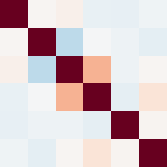
\includegraphics[interpolate=true,width=1.670000in,height=1.670000in]{covariance-matrices-img1.png}}%
\end{pgfscope}%
\begin{pgfscope}%
\pgfsetrectcap%
\pgfsetmiterjoin%
\pgfsetlinewidth{0.501875pt}%
\definecolor{currentstroke}{rgb}{0.000000,0.000000,0.000000}%
\pgfsetstrokecolor{currentstroke}%
\pgfsetdash{}{0pt}%
\pgfpathmoveto{\pgfqpoint{2.045273in}{2.383479in}}%
\pgfpathlineto{\pgfqpoint{2.045273in}{4.046206in}}%
\pgfusepath{stroke}%
\end{pgfscope}%
\begin{pgfscope}%
\pgfsetrectcap%
\pgfsetmiterjoin%
\pgfsetlinewidth{0.501875pt}%
\definecolor{currentstroke}{rgb}{0.000000,0.000000,0.000000}%
\pgfsetstrokecolor{currentstroke}%
\pgfsetdash{}{0pt}%
\pgfpathmoveto{\pgfqpoint{3.708000in}{2.383479in}}%
\pgfpathlineto{\pgfqpoint{3.708000in}{4.046206in}}%
\pgfusepath{stroke}%
\end{pgfscope}%
\begin{pgfscope}%
\pgfsetrectcap%
\pgfsetmiterjoin%
\pgfsetlinewidth{0.501875pt}%
\definecolor{currentstroke}{rgb}{0.000000,0.000000,0.000000}%
\pgfsetstrokecolor{currentstroke}%
\pgfsetdash{}{0pt}%
\pgfpathmoveto{\pgfqpoint{2.045273in}{2.383479in}}%
\pgfpathlineto{\pgfqpoint{3.708000in}{2.383479in}}%
\pgfusepath{stroke}%
\end{pgfscope}%
\begin{pgfscope}%
\pgfsetrectcap%
\pgfsetmiterjoin%
\pgfsetlinewidth{0.501875pt}%
\definecolor{currentstroke}{rgb}{0.000000,0.000000,0.000000}%
\pgfsetstrokecolor{currentstroke}%
\pgfsetdash{}{0pt}%
\pgfpathmoveto{\pgfqpoint{2.045273in}{4.046206in}}%
\pgfpathlineto{\pgfqpoint{3.708000in}{4.046206in}}%
\pgfusepath{stroke}%
\end{pgfscope}%
\begin{pgfscope}%
\pgfsetbuttcap%
\pgfsetmiterjoin%
\definecolor{currentfill}{rgb}{1.000000,1.000000,1.000000}%
\pgfsetfillcolor{currentfill}%
\pgfsetlinewidth{0.000000pt}%
\definecolor{currentstroke}{rgb}{0.000000,0.000000,0.000000}%
\pgfsetstrokecolor{currentstroke}%
\pgfsetstrokeopacity{0.000000}%
\pgfsetdash{}{0pt}%
\pgfpathmoveto{\pgfqpoint{0.050000in}{0.283479in}}%
\pgfpathlineto{\pgfqpoint{1.712727in}{0.283479in}}%
\pgfpathlineto{\pgfqpoint{1.712727in}{1.946206in}}%
\pgfpathlineto{\pgfqpoint{0.050000in}{1.946206in}}%
\pgfpathlineto{\pgfqpoint{0.050000in}{0.283479in}}%
\pgfpathclose%
\pgfusepath{fill}%
\end{pgfscope}%
\begin{pgfscope}%
\pgfpathrectangle{\pgfqpoint{0.050000in}{0.283479in}}{\pgfqpoint{1.662727in}{1.662727in}}%
\pgfusepath{clip}%
\pgfsys@transformshift{0.050000in}{0.283479in}%
\pgftext[left,bottom]{
\includegraphics[interpolate=true,width=1.670000in,height=1.670000in]{covariance-matrices-img2.png}}%
\end{pgfscope}%
\begin{pgfscope}%
\pgfsetrectcap%
\pgfsetmiterjoin%
\pgfsetlinewidth{0.501875pt}%
\definecolor{currentstroke}{rgb}{0.000000,0.000000,0.000000}%
\pgfsetstrokecolor{currentstroke}%
\pgfsetdash{}{0pt}%
\pgfpathmoveto{\pgfqpoint{0.050000in}{0.283479in}}%
\pgfpathlineto{\pgfqpoint{0.050000in}{1.946206in}}%
\pgfusepath{stroke}%
\end{pgfscope}%
\begin{pgfscope}%
\pgfsetrectcap%
\pgfsetmiterjoin%
\pgfsetlinewidth{0.501875pt}%
\definecolor{currentstroke}{rgb}{0.000000,0.000000,0.000000}%
\pgfsetstrokecolor{currentstroke}%
\pgfsetdash{}{0pt}%
\pgfpathmoveto{\pgfqpoint{1.712727in}{0.283479in}}%
\pgfpathlineto{\pgfqpoint{1.712727in}{1.946206in}}%
\pgfusepath{stroke}%
\end{pgfscope}%
\begin{pgfscope}%
\pgfsetrectcap%
\pgfsetmiterjoin%
\pgfsetlinewidth{0.501875pt}%
\definecolor{currentstroke}{rgb}{0.000000,0.000000,0.000000}%
\pgfsetstrokecolor{currentstroke}%
\pgfsetdash{}{0pt}%
\pgfpathmoveto{\pgfqpoint{0.050000in}{0.283479in}}%
\pgfpathlineto{\pgfqpoint{1.712727in}{0.283479in}}%
\pgfusepath{stroke}%
\end{pgfscope}%
\begin{pgfscope}%
\pgfsetrectcap%
\pgfsetmiterjoin%
\pgfsetlinewidth{0.501875pt}%
\definecolor{currentstroke}{rgb}{0.000000,0.000000,0.000000}%
\pgfsetstrokecolor{currentstroke}%
\pgfsetdash{}{0pt}%
\pgfpathmoveto{\pgfqpoint{0.050000in}{1.946206in}}%
\pgfpathlineto{\pgfqpoint{1.712727in}{1.946206in}}%
\pgfusepath{stroke}%
\end{pgfscope}%
\begin{pgfscope}%
\pgfsetbuttcap%
\pgfsetmiterjoin%
\definecolor{currentfill}{rgb}{1.000000,1.000000,1.000000}%
\pgfsetfillcolor{currentfill}%
\pgfsetlinewidth{0.000000pt}%
\definecolor{currentstroke}{rgb}{0.000000,0.000000,0.000000}%
\pgfsetstrokecolor{currentstroke}%
\pgfsetstrokeopacity{0.000000}%
\pgfsetdash{}{0pt}%
\pgfpathmoveto{\pgfqpoint{2.045273in}{0.283479in}}%
\pgfpathlineto{\pgfqpoint{3.708000in}{0.283479in}}%
\pgfpathlineto{\pgfqpoint{3.708000in}{1.946206in}}%
\pgfpathlineto{\pgfqpoint{2.045273in}{1.946206in}}%
\pgfpathlineto{\pgfqpoint{2.045273in}{0.283479in}}%
\pgfpathclose%
\pgfusepath{fill}%
\end{pgfscope}%
\begin{pgfscope}%
\pgfpathrectangle{\pgfqpoint{2.045273in}{0.283479in}}{\pgfqpoint{1.662727in}{1.662727in}}%
\pgfusepath{clip}%
\pgfsys@transformshift{2.045273in}{0.283479in}%
\pgftext[left,bottom]{
\includegraphics[interpolate=true,width=1.670000in,height=1.670000in]{covariance-matrices-img3.png}}%
\end{pgfscope}%
\begin{pgfscope}%
\pgfsetrectcap%
\pgfsetmiterjoin%
\pgfsetlinewidth{0.501875pt}%
\definecolor{currentstroke}{rgb}{0.000000,0.000000,0.000000}%
\pgfsetstrokecolor{currentstroke}%
\pgfsetdash{}{0pt}%
\pgfpathmoveto{\pgfqpoint{2.045273in}{0.283479in}}%
\pgfpathlineto{\pgfqpoint{2.045273in}{1.946206in}}%
\pgfusepath{stroke}%
\end{pgfscope}%
\begin{pgfscope}%
\pgfsetrectcap%
\pgfsetmiterjoin%
\pgfsetlinewidth{0.501875pt}%
\definecolor{currentstroke}{rgb}{0.000000,0.000000,0.000000}%
\pgfsetstrokecolor{currentstroke}%
\pgfsetdash{}{0pt}%
\pgfpathmoveto{\pgfqpoint{3.708000in}{0.283479in}}%
\pgfpathlineto{\pgfqpoint{3.708000in}{1.946206in}}%
\pgfusepath{stroke}%
\end{pgfscope}%
\begin{pgfscope}%
\pgfsetrectcap%
\pgfsetmiterjoin%
\pgfsetlinewidth{0.501875pt}%
\definecolor{currentstroke}{rgb}{0.000000,0.000000,0.000000}%
\pgfsetstrokecolor{currentstroke}%
\pgfsetdash{}{0pt}%
\pgfpathmoveto{\pgfqpoint{2.045273in}{0.283479in}}%
\pgfpathlineto{\pgfqpoint{3.708000in}{0.283479in}}%
\pgfusepath{stroke}%
\end{pgfscope}%
\begin{pgfscope}%
\pgfsetrectcap%
\pgfsetmiterjoin%
\pgfsetlinewidth{0.501875pt}%
\definecolor{currentstroke}{rgb}{0.000000,0.000000,0.000000}%
\pgfsetstrokecolor{currentstroke}%
\pgfsetdash{}{0pt}%
\pgfpathmoveto{\pgfqpoint{2.045273in}{1.946206in}}%
\pgfpathlineto{\pgfqpoint{3.708000in}{1.946206in}}%
\pgfusepath{stroke}%
\end{pgfscope}%
\begin{pgfscope}%
\definecolor{textcolor}{rgb}{0.000000,0.000000,0.000000}%
\pgfsetstrokecolor{textcolor}%
\pgfsetfillcolor{textcolor}%
\pgftext[x=0.881364in,y=2.217206in,,]{\color{textcolor}\rmfamily\fontsize{10.000000}{12.000000}\selectfont (a)}%
\end{pgfscope}%
\begin{pgfscope}%
\definecolor{textcolor}{rgb}{0.000000,0.000000,0.000000}%
\pgfsetstrokecolor{textcolor}%
\pgfsetfillcolor{textcolor}%
\pgftext[x=2.876636in,y=2.217206in,,]{\color{textcolor}\rmfamily\fontsize{10.000000}{12.000000}\selectfont (b)}%
\end{pgfscope}%
\begin{pgfscope}%
\definecolor{textcolor}{rgb}{0.000000,0.000000,0.000000}%
\pgfsetstrokecolor{textcolor}%
\pgfsetfillcolor{textcolor}%
\pgftext[x=0.881364in,y=0.117206in,,]{\color{textcolor}\rmfamily\fontsize{10.000000}{12.000000}\selectfont (c)}%
\end{pgfscope}%
\begin{pgfscope}%
\definecolor{textcolor}{rgb}{0.000000,0.000000,0.000000}%
\pgfsetstrokecolor{textcolor}%
\pgfsetfillcolor{textcolor}%
\pgftext[x=2.876636in,y=0.117206in,,]{\color{textcolor}\rmfamily\fontsize{10.000000}{12.000000}\selectfont (d)}%
\end{pgfscope}%
\begin{pgfscope}%
\pgfsetbuttcap%
\pgfsetmiterjoin%
\definecolor{currentfill}{rgb}{1.000000,1.000000,1.000000}%
\pgfsetfillcolor{currentfill}%
\pgfsetlinewidth{0.000000pt}%
\definecolor{currentstroke}{rgb}{0.000000,0.000000,0.000000}%
\pgfsetstrokecolor{currentstroke}%
\pgfsetstrokeopacity{0.000000}%
\pgfsetdash{}{0pt}%
\pgfpathmoveto{\pgfqpoint{3.936625in}{0.624843in}}%
\pgfpathlineto{\pgfqpoint{4.090625in}{0.624843in}}%
\pgfpathlineto{\pgfqpoint{4.090625in}{3.704843in}}%
\pgfpathlineto{\pgfqpoint{3.936625in}{3.704843in}}%
\pgfpathlineto{\pgfqpoint{3.936625in}{0.624843in}}%
\pgfpathclose%
\pgfusepath{fill}%
\end{pgfscope}%
\begin{pgfscope}%
\pgfpathrectangle{\pgfqpoint{3.936625in}{0.624843in}}{\pgfqpoint{0.154000in}{3.080000in}}%
\pgfusepath{clip}%
\pgfsetbuttcap%
\pgfsetmiterjoin%
\definecolor{currentfill}{rgb}{1.000000,1.000000,1.000000}%
\pgfsetfillcolor{currentfill}%
\pgfsetlinewidth{0.010037pt}%
\definecolor{currentstroke}{rgb}{1.000000,1.000000,1.000000}%
\pgfsetstrokecolor{currentstroke}%
\pgfsetdash{}{0pt}%
\pgfusepath{stroke,fill}%
\end{pgfscope}%
\begin{pgfscope}%
\pgfsys@transformshift{3.940000in}{0.626206in}%
\pgftext[left,bottom]{
\includegraphics[interpolate=true,width=0.150000in,height=3.080000in]{covariance-matrices-img4.png}}%
\end{pgfscope}%
\begin{pgfscope}%
\pgfsetbuttcap%
\pgfsetroundjoin%
\definecolor{currentfill}{rgb}{0.000000,0.000000,0.000000}%
\pgfsetfillcolor{currentfill}%
\pgfsetlinewidth{0.501875pt}%
\definecolor{currentstroke}{rgb}{0.000000,0.000000,0.000000}%
\pgfsetstrokecolor{currentstroke}%
\pgfsetdash{}{0pt}%
\pgfsys@defobject{currentmarker}{\pgfqpoint{-0.041667in}{0.000000in}}{\pgfqpoint{-0.000000in}{0.000000in}}{%
\pgfpathmoveto{\pgfqpoint{-0.000000in}{0.000000in}}%
\pgfpathlineto{\pgfqpoint{-0.041667in}{0.000000in}}%
\pgfusepath{stroke,fill}%
}%
\begin{pgfscope}%
\pgfsys@transformshift{4.090625in}{0.624843in}%
\pgfsys@useobject{currentmarker}{}%
\end{pgfscope}%
\end{pgfscope}%
\begin{pgfscope}%
\definecolor{textcolor}{rgb}{0.000000,0.000000,0.000000}%
\pgfsetstrokecolor{textcolor}%
\pgfsetfillcolor{textcolor}%
\pgftext[x=4.139236in, y=0.572081in, left, base]{\color{textcolor}\rmfamily\fontsize{10.000000}{12.000000}\selectfont \(\displaystyle {\ensuremath{-}1.00}\)}%
\end{pgfscope}%
\begin{pgfscope}%
\pgfsetbuttcap%
\pgfsetroundjoin%
\definecolor{currentfill}{rgb}{0.000000,0.000000,0.000000}%
\pgfsetfillcolor{currentfill}%
\pgfsetlinewidth{0.501875pt}%
\definecolor{currentstroke}{rgb}{0.000000,0.000000,0.000000}%
\pgfsetstrokecolor{currentstroke}%
\pgfsetdash{}{0pt}%
\pgfsys@defobject{currentmarker}{\pgfqpoint{-0.041667in}{0.000000in}}{\pgfqpoint{-0.000000in}{0.000000in}}{%
\pgfpathmoveto{\pgfqpoint{-0.000000in}{0.000000in}}%
\pgfpathlineto{\pgfqpoint{-0.041667in}{0.000000in}}%
\pgfusepath{stroke,fill}%
}%
\begin{pgfscope}%
\pgfsys@transformshift{4.090625in}{1.009843in}%
\pgfsys@useobject{currentmarker}{}%
\end{pgfscope}%
\end{pgfscope}%
\begin{pgfscope}%
\definecolor{textcolor}{rgb}{0.000000,0.000000,0.000000}%
\pgfsetstrokecolor{textcolor}%
\pgfsetfillcolor{textcolor}%
\pgftext[x=4.139236in, y=0.957081in, left, base]{\color{textcolor}\rmfamily\fontsize{10.000000}{12.000000}\selectfont \(\displaystyle {\ensuremath{-}0.75}\)}%
\end{pgfscope}%
\begin{pgfscope}%
\pgfsetbuttcap%
\pgfsetroundjoin%
\definecolor{currentfill}{rgb}{0.000000,0.000000,0.000000}%
\pgfsetfillcolor{currentfill}%
\pgfsetlinewidth{0.501875pt}%
\definecolor{currentstroke}{rgb}{0.000000,0.000000,0.000000}%
\pgfsetstrokecolor{currentstroke}%
\pgfsetdash{}{0pt}%
\pgfsys@defobject{currentmarker}{\pgfqpoint{-0.041667in}{0.000000in}}{\pgfqpoint{-0.000000in}{0.000000in}}{%
\pgfpathmoveto{\pgfqpoint{-0.000000in}{0.000000in}}%
\pgfpathlineto{\pgfqpoint{-0.041667in}{0.000000in}}%
\pgfusepath{stroke,fill}%
}%
\begin{pgfscope}%
\pgfsys@transformshift{4.090625in}{1.394843in}%
\pgfsys@useobject{currentmarker}{}%
\end{pgfscope}%
\end{pgfscope}%
\begin{pgfscope}%
\definecolor{textcolor}{rgb}{0.000000,0.000000,0.000000}%
\pgfsetstrokecolor{textcolor}%
\pgfsetfillcolor{textcolor}%
\pgftext[x=4.139236in, y=1.342081in, left, base]{\color{textcolor}\rmfamily\fontsize{10.000000}{12.000000}\selectfont \(\displaystyle {\ensuremath{-}0.50}\)}%
\end{pgfscope}%
\begin{pgfscope}%
\pgfsetbuttcap%
\pgfsetroundjoin%
\definecolor{currentfill}{rgb}{0.000000,0.000000,0.000000}%
\pgfsetfillcolor{currentfill}%
\pgfsetlinewidth{0.501875pt}%
\definecolor{currentstroke}{rgb}{0.000000,0.000000,0.000000}%
\pgfsetstrokecolor{currentstroke}%
\pgfsetdash{}{0pt}%
\pgfsys@defobject{currentmarker}{\pgfqpoint{-0.041667in}{0.000000in}}{\pgfqpoint{-0.000000in}{0.000000in}}{%
\pgfpathmoveto{\pgfqpoint{-0.000000in}{0.000000in}}%
\pgfpathlineto{\pgfqpoint{-0.041667in}{0.000000in}}%
\pgfusepath{stroke,fill}%
}%
\begin{pgfscope}%
\pgfsys@transformshift{4.090625in}{1.779843in}%
\pgfsys@useobject{currentmarker}{}%
\end{pgfscope}%
\end{pgfscope}%
\begin{pgfscope}%
\definecolor{textcolor}{rgb}{0.000000,0.000000,0.000000}%
\pgfsetstrokecolor{textcolor}%
\pgfsetfillcolor{textcolor}%
\pgftext[x=4.139236in, y=1.727081in, left, base]{\color{textcolor}\rmfamily\fontsize{10.000000}{12.000000}\selectfont \(\displaystyle {\ensuremath{-}0.25}\)}%
\end{pgfscope}%
\begin{pgfscope}%
\pgfsetbuttcap%
\pgfsetroundjoin%
\definecolor{currentfill}{rgb}{0.000000,0.000000,0.000000}%
\pgfsetfillcolor{currentfill}%
\pgfsetlinewidth{0.501875pt}%
\definecolor{currentstroke}{rgb}{0.000000,0.000000,0.000000}%
\pgfsetstrokecolor{currentstroke}%
\pgfsetdash{}{0pt}%
\pgfsys@defobject{currentmarker}{\pgfqpoint{-0.041667in}{0.000000in}}{\pgfqpoint{-0.000000in}{0.000000in}}{%
\pgfpathmoveto{\pgfqpoint{-0.000000in}{0.000000in}}%
\pgfpathlineto{\pgfqpoint{-0.041667in}{0.000000in}}%
\pgfusepath{stroke,fill}%
}%
\begin{pgfscope}%
\pgfsys@transformshift{4.090625in}{2.164843in}%
\pgfsys@useobject{currentmarker}{}%
\end{pgfscope}%
\end{pgfscope}%
\begin{pgfscope}%
\definecolor{textcolor}{rgb}{0.000000,0.000000,0.000000}%
\pgfsetstrokecolor{textcolor}%
\pgfsetfillcolor{textcolor}%
\pgftext[x=4.139236in, y=2.112081in, left, base]{\color{textcolor}\rmfamily\fontsize{10.000000}{12.000000}\selectfont \(\displaystyle {0.00}\)}%
\end{pgfscope}%
\begin{pgfscope}%
\pgfsetbuttcap%
\pgfsetroundjoin%
\definecolor{currentfill}{rgb}{0.000000,0.000000,0.000000}%
\pgfsetfillcolor{currentfill}%
\pgfsetlinewidth{0.501875pt}%
\definecolor{currentstroke}{rgb}{0.000000,0.000000,0.000000}%
\pgfsetstrokecolor{currentstroke}%
\pgfsetdash{}{0pt}%
\pgfsys@defobject{currentmarker}{\pgfqpoint{-0.041667in}{0.000000in}}{\pgfqpoint{-0.000000in}{0.000000in}}{%
\pgfpathmoveto{\pgfqpoint{-0.000000in}{0.000000in}}%
\pgfpathlineto{\pgfqpoint{-0.041667in}{0.000000in}}%
\pgfusepath{stroke,fill}%
}%
\begin{pgfscope}%
\pgfsys@transformshift{4.090625in}{2.549843in}%
\pgfsys@useobject{currentmarker}{}%
\end{pgfscope}%
\end{pgfscope}%
\begin{pgfscope}%
\definecolor{textcolor}{rgb}{0.000000,0.000000,0.000000}%
\pgfsetstrokecolor{textcolor}%
\pgfsetfillcolor{textcolor}%
\pgftext[x=4.139236in, y=2.497081in, left, base]{\color{textcolor}\rmfamily\fontsize{10.000000}{12.000000}\selectfont \(\displaystyle {0.25}\)}%
\end{pgfscope}%
\begin{pgfscope}%
\pgfsetbuttcap%
\pgfsetroundjoin%
\definecolor{currentfill}{rgb}{0.000000,0.000000,0.000000}%
\pgfsetfillcolor{currentfill}%
\pgfsetlinewidth{0.501875pt}%
\definecolor{currentstroke}{rgb}{0.000000,0.000000,0.000000}%
\pgfsetstrokecolor{currentstroke}%
\pgfsetdash{}{0pt}%
\pgfsys@defobject{currentmarker}{\pgfqpoint{-0.041667in}{0.000000in}}{\pgfqpoint{-0.000000in}{0.000000in}}{%
\pgfpathmoveto{\pgfqpoint{-0.000000in}{0.000000in}}%
\pgfpathlineto{\pgfqpoint{-0.041667in}{0.000000in}}%
\pgfusepath{stroke,fill}%
}%
\begin{pgfscope}%
\pgfsys@transformshift{4.090625in}{2.934843in}%
\pgfsys@useobject{currentmarker}{}%
\end{pgfscope}%
\end{pgfscope}%
\begin{pgfscope}%
\definecolor{textcolor}{rgb}{0.000000,0.000000,0.000000}%
\pgfsetstrokecolor{textcolor}%
\pgfsetfillcolor{textcolor}%
\pgftext[x=4.139236in, y=2.882081in, left, base]{\color{textcolor}\rmfamily\fontsize{10.000000}{12.000000}\selectfont \(\displaystyle {0.50}\)}%
\end{pgfscope}%
\begin{pgfscope}%
\pgfsetbuttcap%
\pgfsetroundjoin%
\definecolor{currentfill}{rgb}{0.000000,0.000000,0.000000}%
\pgfsetfillcolor{currentfill}%
\pgfsetlinewidth{0.501875pt}%
\definecolor{currentstroke}{rgb}{0.000000,0.000000,0.000000}%
\pgfsetstrokecolor{currentstroke}%
\pgfsetdash{}{0pt}%
\pgfsys@defobject{currentmarker}{\pgfqpoint{-0.041667in}{0.000000in}}{\pgfqpoint{-0.000000in}{0.000000in}}{%
\pgfpathmoveto{\pgfqpoint{-0.000000in}{0.000000in}}%
\pgfpathlineto{\pgfqpoint{-0.041667in}{0.000000in}}%
\pgfusepath{stroke,fill}%
}%
\begin{pgfscope}%
\pgfsys@transformshift{4.090625in}{3.319843in}%
\pgfsys@useobject{currentmarker}{}%
\end{pgfscope}%
\end{pgfscope}%
\begin{pgfscope}%
\definecolor{textcolor}{rgb}{0.000000,0.000000,0.000000}%
\pgfsetstrokecolor{textcolor}%
\pgfsetfillcolor{textcolor}%
\pgftext[x=4.139236in, y=3.267081in, left, base]{\color{textcolor}\rmfamily\fontsize{10.000000}{12.000000}\selectfont \(\displaystyle {0.75}\)}%
\end{pgfscope}%
\begin{pgfscope}%
\pgfsetbuttcap%
\pgfsetroundjoin%
\definecolor{currentfill}{rgb}{0.000000,0.000000,0.000000}%
\pgfsetfillcolor{currentfill}%
\pgfsetlinewidth{0.501875pt}%
\definecolor{currentstroke}{rgb}{0.000000,0.000000,0.000000}%
\pgfsetstrokecolor{currentstroke}%
\pgfsetdash{}{0pt}%
\pgfsys@defobject{currentmarker}{\pgfqpoint{-0.041667in}{0.000000in}}{\pgfqpoint{-0.000000in}{0.000000in}}{%
\pgfpathmoveto{\pgfqpoint{-0.000000in}{0.000000in}}%
\pgfpathlineto{\pgfqpoint{-0.041667in}{0.000000in}}%
\pgfusepath{stroke,fill}%
}%
\begin{pgfscope}%
\pgfsys@transformshift{4.090625in}{3.704843in}%
\pgfsys@useobject{currentmarker}{}%
\end{pgfscope}%
\end{pgfscope}%
\begin{pgfscope}%
\definecolor{textcolor}{rgb}{0.000000,0.000000,0.000000}%
\pgfsetstrokecolor{textcolor}%
\pgfsetfillcolor{textcolor}%
\pgftext[x=4.139236in, y=3.652081in, left, base]{\color{textcolor}\rmfamily\fontsize{10.000000}{12.000000}\selectfont \(\displaystyle {1.00}\)}%
\end{pgfscope}%
\begin{pgfscope}%
\pgfsetbuttcap%
\pgfsetroundjoin%
\definecolor{currentfill}{rgb}{0.000000,0.000000,0.000000}%
\pgfsetfillcolor{currentfill}%
\pgfsetlinewidth{0.501875pt}%
\definecolor{currentstroke}{rgb}{0.000000,0.000000,0.000000}%
\pgfsetstrokecolor{currentstroke}%
\pgfsetdash{}{0pt}%
\pgfsys@defobject{currentmarker}{\pgfqpoint{-0.020833in}{0.000000in}}{\pgfqpoint{-0.000000in}{0.000000in}}{%
\pgfpathmoveto{\pgfqpoint{-0.000000in}{0.000000in}}%
\pgfpathlineto{\pgfqpoint{-0.020833in}{0.000000in}}%
\pgfusepath{stroke,fill}%
}%
\begin{pgfscope}%
\pgfsys@transformshift{4.090625in}{0.701843in}%
\pgfsys@useobject{currentmarker}{}%
\end{pgfscope}%
\end{pgfscope}%
\begin{pgfscope}%
\pgfsetbuttcap%
\pgfsetroundjoin%
\definecolor{currentfill}{rgb}{0.000000,0.000000,0.000000}%
\pgfsetfillcolor{currentfill}%
\pgfsetlinewidth{0.501875pt}%
\definecolor{currentstroke}{rgb}{0.000000,0.000000,0.000000}%
\pgfsetstrokecolor{currentstroke}%
\pgfsetdash{}{0pt}%
\pgfsys@defobject{currentmarker}{\pgfqpoint{-0.020833in}{0.000000in}}{\pgfqpoint{-0.000000in}{0.000000in}}{%
\pgfpathmoveto{\pgfqpoint{-0.000000in}{0.000000in}}%
\pgfpathlineto{\pgfqpoint{-0.020833in}{0.000000in}}%
\pgfusepath{stroke,fill}%
}%
\begin{pgfscope}%
\pgfsys@transformshift{4.090625in}{0.778843in}%
\pgfsys@useobject{currentmarker}{}%
\end{pgfscope}%
\end{pgfscope}%
\begin{pgfscope}%
\pgfsetbuttcap%
\pgfsetroundjoin%
\definecolor{currentfill}{rgb}{0.000000,0.000000,0.000000}%
\pgfsetfillcolor{currentfill}%
\pgfsetlinewidth{0.501875pt}%
\definecolor{currentstroke}{rgb}{0.000000,0.000000,0.000000}%
\pgfsetstrokecolor{currentstroke}%
\pgfsetdash{}{0pt}%
\pgfsys@defobject{currentmarker}{\pgfqpoint{-0.020833in}{0.000000in}}{\pgfqpoint{-0.000000in}{0.000000in}}{%
\pgfpathmoveto{\pgfqpoint{-0.000000in}{0.000000in}}%
\pgfpathlineto{\pgfqpoint{-0.020833in}{0.000000in}}%
\pgfusepath{stroke,fill}%
}%
\begin{pgfscope}%
\pgfsys@transformshift{4.090625in}{0.855843in}%
\pgfsys@useobject{currentmarker}{}%
\end{pgfscope}%
\end{pgfscope}%
\begin{pgfscope}%
\pgfsetbuttcap%
\pgfsetroundjoin%
\definecolor{currentfill}{rgb}{0.000000,0.000000,0.000000}%
\pgfsetfillcolor{currentfill}%
\pgfsetlinewidth{0.501875pt}%
\definecolor{currentstroke}{rgb}{0.000000,0.000000,0.000000}%
\pgfsetstrokecolor{currentstroke}%
\pgfsetdash{}{0pt}%
\pgfsys@defobject{currentmarker}{\pgfqpoint{-0.020833in}{0.000000in}}{\pgfqpoint{-0.000000in}{0.000000in}}{%
\pgfpathmoveto{\pgfqpoint{-0.000000in}{0.000000in}}%
\pgfpathlineto{\pgfqpoint{-0.020833in}{0.000000in}}%
\pgfusepath{stroke,fill}%
}%
\begin{pgfscope}%
\pgfsys@transformshift{4.090625in}{0.932843in}%
\pgfsys@useobject{currentmarker}{}%
\end{pgfscope}%
\end{pgfscope}%
\begin{pgfscope}%
\pgfsetbuttcap%
\pgfsetroundjoin%
\definecolor{currentfill}{rgb}{0.000000,0.000000,0.000000}%
\pgfsetfillcolor{currentfill}%
\pgfsetlinewidth{0.501875pt}%
\definecolor{currentstroke}{rgb}{0.000000,0.000000,0.000000}%
\pgfsetstrokecolor{currentstroke}%
\pgfsetdash{}{0pt}%
\pgfsys@defobject{currentmarker}{\pgfqpoint{-0.020833in}{0.000000in}}{\pgfqpoint{-0.000000in}{0.000000in}}{%
\pgfpathmoveto{\pgfqpoint{-0.000000in}{0.000000in}}%
\pgfpathlineto{\pgfqpoint{-0.020833in}{0.000000in}}%
\pgfusepath{stroke,fill}%
}%
\begin{pgfscope}%
\pgfsys@transformshift{4.090625in}{1.086843in}%
\pgfsys@useobject{currentmarker}{}%
\end{pgfscope}%
\end{pgfscope}%
\begin{pgfscope}%
\pgfsetbuttcap%
\pgfsetroundjoin%
\definecolor{currentfill}{rgb}{0.000000,0.000000,0.000000}%
\pgfsetfillcolor{currentfill}%
\pgfsetlinewidth{0.501875pt}%
\definecolor{currentstroke}{rgb}{0.000000,0.000000,0.000000}%
\pgfsetstrokecolor{currentstroke}%
\pgfsetdash{}{0pt}%
\pgfsys@defobject{currentmarker}{\pgfqpoint{-0.020833in}{0.000000in}}{\pgfqpoint{-0.000000in}{0.000000in}}{%
\pgfpathmoveto{\pgfqpoint{-0.000000in}{0.000000in}}%
\pgfpathlineto{\pgfqpoint{-0.020833in}{0.000000in}}%
\pgfusepath{stroke,fill}%
}%
\begin{pgfscope}%
\pgfsys@transformshift{4.090625in}{1.163843in}%
\pgfsys@useobject{currentmarker}{}%
\end{pgfscope}%
\end{pgfscope}%
\begin{pgfscope}%
\pgfsetbuttcap%
\pgfsetroundjoin%
\definecolor{currentfill}{rgb}{0.000000,0.000000,0.000000}%
\pgfsetfillcolor{currentfill}%
\pgfsetlinewidth{0.501875pt}%
\definecolor{currentstroke}{rgb}{0.000000,0.000000,0.000000}%
\pgfsetstrokecolor{currentstroke}%
\pgfsetdash{}{0pt}%
\pgfsys@defobject{currentmarker}{\pgfqpoint{-0.020833in}{0.000000in}}{\pgfqpoint{-0.000000in}{0.000000in}}{%
\pgfpathmoveto{\pgfqpoint{-0.000000in}{0.000000in}}%
\pgfpathlineto{\pgfqpoint{-0.020833in}{0.000000in}}%
\pgfusepath{stroke,fill}%
}%
\begin{pgfscope}%
\pgfsys@transformshift{4.090625in}{1.240843in}%
\pgfsys@useobject{currentmarker}{}%
\end{pgfscope}%
\end{pgfscope}%
\begin{pgfscope}%
\pgfsetbuttcap%
\pgfsetroundjoin%
\definecolor{currentfill}{rgb}{0.000000,0.000000,0.000000}%
\pgfsetfillcolor{currentfill}%
\pgfsetlinewidth{0.501875pt}%
\definecolor{currentstroke}{rgb}{0.000000,0.000000,0.000000}%
\pgfsetstrokecolor{currentstroke}%
\pgfsetdash{}{0pt}%
\pgfsys@defobject{currentmarker}{\pgfqpoint{-0.020833in}{0.000000in}}{\pgfqpoint{-0.000000in}{0.000000in}}{%
\pgfpathmoveto{\pgfqpoint{-0.000000in}{0.000000in}}%
\pgfpathlineto{\pgfqpoint{-0.020833in}{0.000000in}}%
\pgfusepath{stroke,fill}%
}%
\begin{pgfscope}%
\pgfsys@transformshift{4.090625in}{1.317843in}%
\pgfsys@useobject{currentmarker}{}%
\end{pgfscope}%
\end{pgfscope}%
\begin{pgfscope}%
\pgfsetbuttcap%
\pgfsetroundjoin%
\definecolor{currentfill}{rgb}{0.000000,0.000000,0.000000}%
\pgfsetfillcolor{currentfill}%
\pgfsetlinewidth{0.501875pt}%
\definecolor{currentstroke}{rgb}{0.000000,0.000000,0.000000}%
\pgfsetstrokecolor{currentstroke}%
\pgfsetdash{}{0pt}%
\pgfsys@defobject{currentmarker}{\pgfqpoint{-0.020833in}{0.000000in}}{\pgfqpoint{-0.000000in}{0.000000in}}{%
\pgfpathmoveto{\pgfqpoint{-0.000000in}{0.000000in}}%
\pgfpathlineto{\pgfqpoint{-0.020833in}{0.000000in}}%
\pgfusepath{stroke,fill}%
}%
\begin{pgfscope}%
\pgfsys@transformshift{4.090625in}{1.471843in}%
\pgfsys@useobject{currentmarker}{}%
\end{pgfscope}%
\end{pgfscope}%
\begin{pgfscope}%
\pgfsetbuttcap%
\pgfsetroundjoin%
\definecolor{currentfill}{rgb}{0.000000,0.000000,0.000000}%
\pgfsetfillcolor{currentfill}%
\pgfsetlinewidth{0.501875pt}%
\definecolor{currentstroke}{rgb}{0.000000,0.000000,0.000000}%
\pgfsetstrokecolor{currentstroke}%
\pgfsetdash{}{0pt}%
\pgfsys@defobject{currentmarker}{\pgfqpoint{-0.020833in}{0.000000in}}{\pgfqpoint{-0.000000in}{0.000000in}}{%
\pgfpathmoveto{\pgfqpoint{-0.000000in}{0.000000in}}%
\pgfpathlineto{\pgfqpoint{-0.020833in}{0.000000in}}%
\pgfusepath{stroke,fill}%
}%
\begin{pgfscope}%
\pgfsys@transformshift{4.090625in}{1.548843in}%
\pgfsys@useobject{currentmarker}{}%
\end{pgfscope}%
\end{pgfscope}%
\begin{pgfscope}%
\pgfsetbuttcap%
\pgfsetroundjoin%
\definecolor{currentfill}{rgb}{0.000000,0.000000,0.000000}%
\pgfsetfillcolor{currentfill}%
\pgfsetlinewidth{0.501875pt}%
\definecolor{currentstroke}{rgb}{0.000000,0.000000,0.000000}%
\pgfsetstrokecolor{currentstroke}%
\pgfsetdash{}{0pt}%
\pgfsys@defobject{currentmarker}{\pgfqpoint{-0.020833in}{0.000000in}}{\pgfqpoint{-0.000000in}{0.000000in}}{%
\pgfpathmoveto{\pgfqpoint{-0.000000in}{0.000000in}}%
\pgfpathlineto{\pgfqpoint{-0.020833in}{0.000000in}}%
\pgfusepath{stroke,fill}%
}%
\begin{pgfscope}%
\pgfsys@transformshift{4.090625in}{1.625843in}%
\pgfsys@useobject{currentmarker}{}%
\end{pgfscope}%
\end{pgfscope}%
\begin{pgfscope}%
\pgfsetbuttcap%
\pgfsetroundjoin%
\definecolor{currentfill}{rgb}{0.000000,0.000000,0.000000}%
\pgfsetfillcolor{currentfill}%
\pgfsetlinewidth{0.501875pt}%
\definecolor{currentstroke}{rgb}{0.000000,0.000000,0.000000}%
\pgfsetstrokecolor{currentstroke}%
\pgfsetdash{}{0pt}%
\pgfsys@defobject{currentmarker}{\pgfqpoint{-0.020833in}{0.000000in}}{\pgfqpoint{-0.000000in}{0.000000in}}{%
\pgfpathmoveto{\pgfqpoint{-0.000000in}{0.000000in}}%
\pgfpathlineto{\pgfqpoint{-0.020833in}{0.000000in}}%
\pgfusepath{stroke,fill}%
}%
\begin{pgfscope}%
\pgfsys@transformshift{4.090625in}{1.702843in}%
\pgfsys@useobject{currentmarker}{}%
\end{pgfscope}%
\end{pgfscope}%
\begin{pgfscope}%
\pgfsetbuttcap%
\pgfsetroundjoin%
\definecolor{currentfill}{rgb}{0.000000,0.000000,0.000000}%
\pgfsetfillcolor{currentfill}%
\pgfsetlinewidth{0.501875pt}%
\definecolor{currentstroke}{rgb}{0.000000,0.000000,0.000000}%
\pgfsetstrokecolor{currentstroke}%
\pgfsetdash{}{0pt}%
\pgfsys@defobject{currentmarker}{\pgfqpoint{-0.020833in}{0.000000in}}{\pgfqpoint{-0.000000in}{0.000000in}}{%
\pgfpathmoveto{\pgfqpoint{-0.000000in}{0.000000in}}%
\pgfpathlineto{\pgfqpoint{-0.020833in}{0.000000in}}%
\pgfusepath{stroke,fill}%
}%
\begin{pgfscope}%
\pgfsys@transformshift{4.090625in}{1.856843in}%
\pgfsys@useobject{currentmarker}{}%
\end{pgfscope}%
\end{pgfscope}%
\begin{pgfscope}%
\pgfsetbuttcap%
\pgfsetroundjoin%
\definecolor{currentfill}{rgb}{0.000000,0.000000,0.000000}%
\pgfsetfillcolor{currentfill}%
\pgfsetlinewidth{0.501875pt}%
\definecolor{currentstroke}{rgb}{0.000000,0.000000,0.000000}%
\pgfsetstrokecolor{currentstroke}%
\pgfsetdash{}{0pt}%
\pgfsys@defobject{currentmarker}{\pgfqpoint{-0.020833in}{0.000000in}}{\pgfqpoint{-0.000000in}{0.000000in}}{%
\pgfpathmoveto{\pgfqpoint{-0.000000in}{0.000000in}}%
\pgfpathlineto{\pgfqpoint{-0.020833in}{0.000000in}}%
\pgfusepath{stroke,fill}%
}%
\begin{pgfscope}%
\pgfsys@transformshift{4.090625in}{1.933843in}%
\pgfsys@useobject{currentmarker}{}%
\end{pgfscope}%
\end{pgfscope}%
\begin{pgfscope}%
\pgfsetbuttcap%
\pgfsetroundjoin%
\definecolor{currentfill}{rgb}{0.000000,0.000000,0.000000}%
\pgfsetfillcolor{currentfill}%
\pgfsetlinewidth{0.501875pt}%
\definecolor{currentstroke}{rgb}{0.000000,0.000000,0.000000}%
\pgfsetstrokecolor{currentstroke}%
\pgfsetdash{}{0pt}%
\pgfsys@defobject{currentmarker}{\pgfqpoint{-0.020833in}{0.000000in}}{\pgfqpoint{-0.000000in}{0.000000in}}{%
\pgfpathmoveto{\pgfqpoint{-0.000000in}{0.000000in}}%
\pgfpathlineto{\pgfqpoint{-0.020833in}{0.000000in}}%
\pgfusepath{stroke,fill}%
}%
\begin{pgfscope}%
\pgfsys@transformshift{4.090625in}{2.010843in}%
\pgfsys@useobject{currentmarker}{}%
\end{pgfscope}%
\end{pgfscope}%
\begin{pgfscope}%
\pgfsetbuttcap%
\pgfsetroundjoin%
\definecolor{currentfill}{rgb}{0.000000,0.000000,0.000000}%
\pgfsetfillcolor{currentfill}%
\pgfsetlinewidth{0.501875pt}%
\definecolor{currentstroke}{rgb}{0.000000,0.000000,0.000000}%
\pgfsetstrokecolor{currentstroke}%
\pgfsetdash{}{0pt}%
\pgfsys@defobject{currentmarker}{\pgfqpoint{-0.020833in}{0.000000in}}{\pgfqpoint{-0.000000in}{0.000000in}}{%
\pgfpathmoveto{\pgfqpoint{-0.000000in}{0.000000in}}%
\pgfpathlineto{\pgfqpoint{-0.020833in}{0.000000in}}%
\pgfusepath{stroke,fill}%
}%
\begin{pgfscope}%
\pgfsys@transformshift{4.090625in}{2.087843in}%
\pgfsys@useobject{currentmarker}{}%
\end{pgfscope}%
\end{pgfscope}%
\begin{pgfscope}%
\pgfsetbuttcap%
\pgfsetroundjoin%
\definecolor{currentfill}{rgb}{0.000000,0.000000,0.000000}%
\pgfsetfillcolor{currentfill}%
\pgfsetlinewidth{0.501875pt}%
\definecolor{currentstroke}{rgb}{0.000000,0.000000,0.000000}%
\pgfsetstrokecolor{currentstroke}%
\pgfsetdash{}{0pt}%
\pgfsys@defobject{currentmarker}{\pgfqpoint{-0.020833in}{0.000000in}}{\pgfqpoint{-0.000000in}{0.000000in}}{%
\pgfpathmoveto{\pgfqpoint{-0.000000in}{0.000000in}}%
\pgfpathlineto{\pgfqpoint{-0.020833in}{0.000000in}}%
\pgfusepath{stroke,fill}%
}%
\begin{pgfscope}%
\pgfsys@transformshift{4.090625in}{2.241843in}%
\pgfsys@useobject{currentmarker}{}%
\end{pgfscope}%
\end{pgfscope}%
\begin{pgfscope}%
\pgfsetbuttcap%
\pgfsetroundjoin%
\definecolor{currentfill}{rgb}{0.000000,0.000000,0.000000}%
\pgfsetfillcolor{currentfill}%
\pgfsetlinewidth{0.501875pt}%
\definecolor{currentstroke}{rgb}{0.000000,0.000000,0.000000}%
\pgfsetstrokecolor{currentstroke}%
\pgfsetdash{}{0pt}%
\pgfsys@defobject{currentmarker}{\pgfqpoint{-0.020833in}{0.000000in}}{\pgfqpoint{-0.000000in}{0.000000in}}{%
\pgfpathmoveto{\pgfqpoint{-0.000000in}{0.000000in}}%
\pgfpathlineto{\pgfqpoint{-0.020833in}{0.000000in}}%
\pgfusepath{stroke,fill}%
}%
\begin{pgfscope}%
\pgfsys@transformshift{4.090625in}{2.318843in}%
\pgfsys@useobject{currentmarker}{}%
\end{pgfscope}%
\end{pgfscope}%
\begin{pgfscope}%
\pgfsetbuttcap%
\pgfsetroundjoin%
\definecolor{currentfill}{rgb}{0.000000,0.000000,0.000000}%
\pgfsetfillcolor{currentfill}%
\pgfsetlinewidth{0.501875pt}%
\definecolor{currentstroke}{rgb}{0.000000,0.000000,0.000000}%
\pgfsetstrokecolor{currentstroke}%
\pgfsetdash{}{0pt}%
\pgfsys@defobject{currentmarker}{\pgfqpoint{-0.020833in}{0.000000in}}{\pgfqpoint{-0.000000in}{0.000000in}}{%
\pgfpathmoveto{\pgfqpoint{-0.000000in}{0.000000in}}%
\pgfpathlineto{\pgfqpoint{-0.020833in}{0.000000in}}%
\pgfusepath{stroke,fill}%
}%
\begin{pgfscope}%
\pgfsys@transformshift{4.090625in}{2.395843in}%
\pgfsys@useobject{currentmarker}{}%
\end{pgfscope}%
\end{pgfscope}%
\begin{pgfscope}%
\pgfsetbuttcap%
\pgfsetroundjoin%
\definecolor{currentfill}{rgb}{0.000000,0.000000,0.000000}%
\pgfsetfillcolor{currentfill}%
\pgfsetlinewidth{0.501875pt}%
\definecolor{currentstroke}{rgb}{0.000000,0.000000,0.000000}%
\pgfsetstrokecolor{currentstroke}%
\pgfsetdash{}{0pt}%
\pgfsys@defobject{currentmarker}{\pgfqpoint{-0.020833in}{0.000000in}}{\pgfqpoint{-0.000000in}{0.000000in}}{%
\pgfpathmoveto{\pgfqpoint{-0.000000in}{0.000000in}}%
\pgfpathlineto{\pgfqpoint{-0.020833in}{0.000000in}}%
\pgfusepath{stroke,fill}%
}%
\begin{pgfscope}%
\pgfsys@transformshift{4.090625in}{2.472843in}%
\pgfsys@useobject{currentmarker}{}%
\end{pgfscope}%
\end{pgfscope}%
\begin{pgfscope}%
\pgfsetbuttcap%
\pgfsetroundjoin%
\definecolor{currentfill}{rgb}{0.000000,0.000000,0.000000}%
\pgfsetfillcolor{currentfill}%
\pgfsetlinewidth{0.501875pt}%
\definecolor{currentstroke}{rgb}{0.000000,0.000000,0.000000}%
\pgfsetstrokecolor{currentstroke}%
\pgfsetdash{}{0pt}%
\pgfsys@defobject{currentmarker}{\pgfqpoint{-0.020833in}{0.000000in}}{\pgfqpoint{-0.000000in}{0.000000in}}{%
\pgfpathmoveto{\pgfqpoint{-0.000000in}{0.000000in}}%
\pgfpathlineto{\pgfqpoint{-0.020833in}{0.000000in}}%
\pgfusepath{stroke,fill}%
}%
\begin{pgfscope}%
\pgfsys@transformshift{4.090625in}{2.626843in}%
\pgfsys@useobject{currentmarker}{}%
\end{pgfscope}%
\end{pgfscope}%
\begin{pgfscope}%
\pgfsetbuttcap%
\pgfsetroundjoin%
\definecolor{currentfill}{rgb}{0.000000,0.000000,0.000000}%
\pgfsetfillcolor{currentfill}%
\pgfsetlinewidth{0.501875pt}%
\definecolor{currentstroke}{rgb}{0.000000,0.000000,0.000000}%
\pgfsetstrokecolor{currentstroke}%
\pgfsetdash{}{0pt}%
\pgfsys@defobject{currentmarker}{\pgfqpoint{-0.020833in}{0.000000in}}{\pgfqpoint{-0.000000in}{0.000000in}}{%
\pgfpathmoveto{\pgfqpoint{-0.000000in}{0.000000in}}%
\pgfpathlineto{\pgfqpoint{-0.020833in}{0.000000in}}%
\pgfusepath{stroke,fill}%
}%
\begin{pgfscope}%
\pgfsys@transformshift{4.090625in}{2.703843in}%
\pgfsys@useobject{currentmarker}{}%
\end{pgfscope}%
\end{pgfscope}%
\begin{pgfscope}%
\pgfsetbuttcap%
\pgfsetroundjoin%
\definecolor{currentfill}{rgb}{0.000000,0.000000,0.000000}%
\pgfsetfillcolor{currentfill}%
\pgfsetlinewidth{0.501875pt}%
\definecolor{currentstroke}{rgb}{0.000000,0.000000,0.000000}%
\pgfsetstrokecolor{currentstroke}%
\pgfsetdash{}{0pt}%
\pgfsys@defobject{currentmarker}{\pgfqpoint{-0.020833in}{0.000000in}}{\pgfqpoint{-0.000000in}{0.000000in}}{%
\pgfpathmoveto{\pgfqpoint{-0.000000in}{0.000000in}}%
\pgfpathlineto{\pgfqpoint{-0.020833in}{0.000000in}}%
\pgfusepath{stroke,fill}%
}%
\begin{pgfscope}%
\pgfsys@transformshift{4.090625in}{2.780843in}%
\pgfsys@useobject{currentmarker}{}%
\end{pgfscope}%
\end{pgfscope}%
\begin{pgfscope}%
\pgfsetbuttcap%
\pgfsetroundjoin%
\definecolor{currentfill}{rgb}{0.000000,0.000000,0.000000}%
\pgfsetfillcolor{currentfill}%
\pgfsetlinewidth{0.501875pt}%
\definecolor{currentstroke}{rgb}{0.000000,0.000000,0.000000}%
\pgfsetstrokecolor{currentstroke}%
\pgfsetdash{}{0pt}%
\pgfsys@defobject{currentmarker}{\pgfqpoint{-0.020833in}{0.000000in}}{\pgfqpoint{-0.000000in}{0.000000in}}{%
\pgfpathmoveto{\pgfqpoint{-0.000000in}{0.000000in}}%
\pgfpathlineto{\pgfqpoint{-0.020833in}{0.000000in}}%
\pgfusepath{stroke,fill}%
}%
\begin{pgfscope}%
\pgfsys@transformshift{4.090625in}{2.857843in}%
\pgfsys@useobject{currentmarker}{}%
\end{pgfscope}%
\end{pgfscope}%
\begin{pgfscope}%
\pgfsetbuttcap%
\pgfsetroundjoin%
\definecolor{currentfill}{rgb}{0.000000,0.000000,0.000000}%
\pgfsetfillcolor{currentfill}%
\pgfsetlinewidth{0.501875pt}%
\definecolor{currentstroke}{rgb}{0.000000,0.000000,0.000000}%
\pgfsetstrokecolor{currentstroke}%
\pgfsetdash{}{0pt}%
\pgfsys@defobject{currentmarker}{\pgfqpoint{-0.020833in}{0.000000in}}{\pgfqpoint{-0.000000in}{0.000000in}}{%
\pgfpathmoveto{\pgfqpoint{-0.000000in}{0.000000in}}%
\pgfpathlineto{\pgfqpoint{-0.020833in}{0.000000in}}%
\pgfusepath{stroke,fill}%
}%
\begin{pgfscope}%
\pgfsys@transformshift{4.090625in}{3.011843in}%
\pgfsys@useobject{currentmarker}{}%
\end{pgfscope}%
\end{pgfscope}%
\begin{pgfscope}%
\pgfsetbuttcap%
\pgfsetroundjoin%
\definecolor{currentfill}{rgb}{0.000000,0.000000,0.000000}%
\pgfsetfillcolor{currentfill}%
\pgfsetlinewidth{0.501875pt}%
\definecolor{currentstroke}{rgb}{0.000000,0.000000,0.000000}%
\pgfsetstrokecolor{currentstroke}%
\pgfsetdash{}{0pt}%
\pgfsys@defobject{currentmarker}{\pgfqpoint{-0.020833in}{0.000000in}}{\pgfqpoint{-0.000000in}{0.000000in}}{%
\pgfpathmoveto{\pgfqpoint{-0.000000in}{0.000000in}}%
\pgfpathlineto{\pgfqpoint{-0.020833in}{0.000000in}}%
\pgfusepath{stroke,fill}%
}%
\begin{pgfscope}%
\pgfsys@transformshift{4.090625in}{3.088843in}%
\pgfsys@useobject{currentmarker}{}%
\end{pgfscope}%
\end{pgfscope}%
\begin{pgfscope}%
\pgfsetbuttcap%
\pgfsetroundjoin%
\definecolor{currentfill}{rgb}{0.000000,0.000000,0.000000}%
\pgfsetfillcolor{currentfill}%
\pgfsetlinewidth{0.501875pt}%
\definecolor{currentstroke}{rgb}{0.000000,0.000000,0.000000}%
\pgfsetstrokecolor{currentstroke}%
\pgfsetdash{}{0pt}%
\pgfsys@defobject{currentmarker}{\pgfqpoint{-0.020833in}{0.000000in}}{\pgfqpoint{-0.000000in}{0.000000in}}{%
\pgfpathmoveto{\pgfqpoint{-0.000000in}{0.000000in}}%
\pgfpathlineto{\pgfqpoint{-0.020833in}{0.000000in}}%
\pgfusepath{stroke,fill}%
}%
\begin{pgfscope}%
\pgfsys@transformshift{4.090625in}{3.165843in}%
\pgfsys@useobject{currentmarker}{}%
\end{pgfscope}%
\end{pgfscope}%
\begin{pgfscope}%
\pgfsetbuttcap%
\pgfsetroundjoin%
\definecolor{currentfill}{rgb}{0.000000,0.000000,0.000000}%
\pgfsetfillcolor{currentfill}%
\pgfsetlinewidth{0.501875pt}%
\definecolor{currentstroke}{rgb}{0.000000,0.000000,0.000000}%
\pgfsetstrokecolor{currentstroke}%
\pgfsetdash{}{0pt}%
\pgfsys@defobject{currentmarker}{\pgfqpoint{-0.020833in}{0.000000in}}{\pgfqpoint{-0.000000in}{0.000000in}}{%
\pgfpathmoveto{\pgfqpoint{-0.000000in}{0.000000in}}%
\pgfpathlineto{\pgfqpoint{-0.020833in}{0.000000in}}%
\pgfusepath{stroke,fill}%
}%
\begin{pgfscope}%
\pgfsys@transformshift{4.090625in}{3.242843in}%
\pgfsys@useobject{currentmarker}{}%
\end{pgfscope}%
\end{pgfscope}%
\begin{pgfscope}%
\pgfsetbuttcap%
\pgfsetroundjoin%
\definecolor{currentfill}{rgb}{0.000000,0.000000,0.000000}%
\pgfsetfillcolor{currentfill}%
\pgfsetlinewidth{0.501875pt}%
\definecolor{currentstroke}{rgb}{0.000000,0.000000,0.000000}%
\pgfsetstrokecolor{currentstroke}%
\pgfsetdash{}{0pt}%
\pgfsys@defobject{currentmarker}{\pgfqpoint{-0.020833in}{0.000000in}}{\pgfqpoint{-0.000000in}{0.000000in}}{%
\pgfpathmoveto{\pgfqpoint{-0.000000in}{0.000000in}}%
\pgfpathlineto{\pgfqpoint{-0.020833in}{0.000000in}}%
\pgfusepath{stroke,fill}%
}%
\begin{pgfscope}%
\pgfsys@transformshift{4.090625in}{3.396843in}%
\pgfsys@useobject{currentmarker}{}%
\end{pgfscope}%
\end{pgfscope}%
\begin{pgfscope}%
\pgfsetbuttcap%
\pgfsetroundjoin%
\definecolor{currentfill}{rgb}{0.000000,0.000000,0.000000}%
\pgfsetfillcolor{currentfill}%
\pgfsetlinewidth{0.501875pt}%
\definecolor{currentstroke}{rgb}{0.000000,0.000000,0.000000}%
\pgfsetstrokecolor{currentstroke}%
\pgfsetdash{}{0pt}%
\pgfsys@defobject{currentmarker}{\pgfqpoint{-0.020833in}{0.000000in}}{\pgfqpoint{-0.000000in}{0.000000in}}{%
\pgfpathmoveto{\pgfqpoint{-0.000000in}{0.000000in}}%
\pgfpathlineto{\pgfqpoint{-0.020833in}{0.000000in}}%
\pgfusepath{stroke,fill}%
}%
\begin{pgfscope}%
\pgfsys@transformshift{4.090625in}{3.473843in}%
\pgfsys@useobject{currentmarker}{}%
\end{pgfscope}%
\end{pgfscope}%
\begin{pgfscope}%
\pgfsetbuttcap%
\pgfsetroundjoin%
\definecolor{currentfill}{rgb}{0.000000,0.000000,0.000000}%
\pgfsetfillcolor{currentfill}%
\pgfsetlinewidth{0.501875pt}%
\definecolor{currentstroke}{rgb}{0.000000,0.000000,0.000000}%
\pgfsetstrokecolor{currentstroke}%
\pgfsetdash{}{0pt}%
\pgfsys@defobject{currentmarker}{\pgfqpoint{-0.020833in}{0.000000in}}{\pgfqpoint{-0.000000in}{0.000000in}}{%
\pgfpathmoveto{\pgfqpoint{-0.000000in}{0.000000in}}%
\pgfpathlineto{\pgfqpoint{-0.020833in}{0.000000in}}%
\pgfusepath{stroke,fill}%
}%
\begin{pgfscope}%
\pgfsys@transformshift{4.090625in}{3.550843in}%
\pgfsys@useobject{currentmarker}{}%
\end{pgfscope}%
\end{pgfscope}%
\begin{pgfscope}%
\pgfsetbuttcap%
\pgfsetroundjoin%
\definecolor{currentfill}{rgb}{0.000000,0.000000,0.000000}%
\pgfsetfillcolor{currentfill}%
\pgfsetlinewidth{0.501875pt}%
\definecolor{currentstroke}{rgb}{0.000000,0.000000,0.000000}%
\pgfsetstrokecolor{currentstroke}%
\pgfsetdash{}{0pt}%
\pgfsys@defobject{currentmarker}{\pgfqpoint{-0.020833in}{0.000000in}}{\pgfqpoint{-0.000000in}{0.000000in}}{%
\pgfpathmoveto{\pgfqpoint{-0.000000in}{0.000000in}}%
\pgfpathlineto{\pgfqpoint{-0.020833in}{0.000000in}}%
\pgfusepath{stroke,fill}%
}%
\begin{pgfscope}%
\pgfsys@transformshift{4.090625in}{3.627843in}%
\pgfsys@useobject{currentmarker}{}%
\end{pgfscope}%
\end{pgfscope}%
\begin{pgfscope}%
\pgfsetrectcap%
\pgfsetmiterjoin%
\pgfsetlinewidth{0.501875pt}%
\definecolor{currentstroke}{rgb}{0.000000,0.000000,0.000000}%
\pgfsetstrokecolor{currentstroke}%
\pgfsetdash{}{0pt}%
\pgfpathmoveto{\pgfqpoint{3.936625in}{0.624843in}}%
\pgfpathlineto{\pgfqpoint{4.013625in}{0.624843in}}%
\pgfpathlineto{\pgfqpoint{4.090625in}{0.624843in}}%
\pgfpathlineto{\pgfqpoint{4.090625in}{3.704843in}}%
\pgfpathlineto{\pgfqpoint{4.013625in}{3.704843in}}%
\pgfpathlineto{\pgfqpoint{3.936625in}{3.704843in}}%
\pgfpathlineto{\pgfqpoint{3.936625in}{0.624843in}}%
\pgfpathclose%
\pgfusepath{stroke}%
\end{pgfscope}%
\end{pgfpicture}%
\makeatother%
\endgroup%

	\caption[Korrelationsmatrizen der transformierten Daten $\mat{Y}$ für den FER-Datensatz von vier Methoden]{Hier sind die Korrelationsmatrizen der transformierten Daten $\mat{Y}$ für den FER-Datensatz abgebildet, wobei in \captiona die Hauptkomponentenanalyse, in \captionb ein linearer dreischichtiger Autoencoder, in \captionc ein nichtlinearer dreischichtiger Autoencoder, wobei der der Encoder eine Sigmoid-Aktivierungsfunktion einsetzt und der Decoder linear ist und in \captiond ein dreischichtiger Autoencoder mit ausschließlich Sigmoid-Aktivierungsfunktionen verwendet wurde, um die Daten auf sechs Dimensionen zu reduzieren. Die Korrelationsmatrix bei Transformation mittels der Hauptkomponentenanalyse ist per Konstruktion eine Einheitsmatrix, das heißt es besteht keine Korrelation in $\mat{Y}$. Bei Transformation durch die Autoencoder besteht Korrelation, wobei der lineare Autoencoder in diesem Fall betragsmäßig kleinere Korrelationen erzeugt als die nichtlinearen Autoencoder. (Eigene Darstellung, angelehnt an \textcite[5]{Plaut.2018})}
	\label{fig:Korrelationsmatrizen}
\end{figure}
Punkt 1 ist in beispielsweise in \figref{fig:Korrelationsmatrizen} zu erkennen. Dargestellt sind die Korrelationsmatrizen der transformierten Daten, wobei in \captiona die Hauptkomponentenanalyse, in \captionb ein linearer dreischichtiger Autoencoder und in \captionc und (d) nichtlineare Autoencoder verwendet wurden. Die Korrelationsmatrix der Hauptkomponentenanalyse ist eine Einheitsmatrix, während die Korrelationsmatrizen der durch die Autoencoder gefundenen latenten Repräsentation von Null verschiedene Werte auf der Nicht-diagonalen aufweisen.

Um die gefundenen Lösungen einer Hauptkomponentenanalyse und von Autoencodern genauer betrachten zu
können, kann die Ladungsmatrix $\mat{A}$ mit den Gewichtsmatrizen eines dreischichtigen
Autoencoders verglichen werden. Im Falle eines dreischichtigen Autoencoders sind die Gewichte des
Encoders eine Matrix $\mat{W}_2 \in \real^{d \times D}$ und die Gewichte des Decoders eine Matrix
$\mat{W}_2 \in \real^{D \times d}$. Auf Bilddatensätzen können diese Matrizen so umgeformt werden,
dass sich für jede Zeile von $\mat{W}_1$ oder Spalte von $\mat{W}_2$ ein Bild ergibt. Auf diese
Weise kann die \enquote{Arbeitsweise} des Autoencoders anschaulich untersucht werden.
\figref{fig:Gewichtsvergleich} setzt dieses Vorgehen auf dem FER-Datensatz um.
\begin{figure}[ht]
	\centering
	%% Creator: Matplotlib, PGF backend
%%
%% To include the figure in your LaTeX document, write
%%   \input{<filename>.pgf}
%%
%% Make sure the required packages are loaded in your preamble
%%   \usepackage{pgf}
%%
%% Also ensure that all the required font packages are loaded; for instance,
%% the lmodern package is sometimes necessary when using math font.
%%   \usepackage{lmodern}
%%
%% Figures using additional raster images can only be included by \input if
%% they are in the same directory as the main LaTeX file. For loading figures
%% from other directories you can use the `import` package
%%   \usepackage{import}
%%
%% and then include the figures with
%%   \import{<path to file>}{<filename>.pgf}
%%
%% Matplotlib used the following preamble
%%   
%%   \usepackage{fontspec}
%%   \setmainfont{DejaVuSerif.ttf}[Path=\detokenize{/Users/moritzmistol/.pyenv/versions/3.9.13/envs/thesis/lib/python3.9/site-packages/matplotlib/mpl-data/fonts/ttf/}]
%%   \setsansfont{DejaVuSans.ttf}[Path=\detokenize{/Users/moritzmistol/.pyenv/versions/3.9.13/envs/thesis/lib/python3.9/site-packages/matplotlib/mpl-data/fonts/ttf/}]
%%   \setmonofont{DejaVuSansMono.ttf}[Path=\detokenize{/Users/moritzmistol/.pyenv/versions/3.9.13/envs/thesis/lib/python3.9/site-packages/matplotlib/mpl-data/fonts/ttf/}]
%%   \makeatletter\@ifpackageloaded{underscore}{}{\usepackage[strings]{underscore}}\makeatother
%%
\begingroup%
\makeatletter%
\begin{pgfpicture}%
\pgfpathrectangle{\pgfpointorigin}{\pgfqpoint{5.544109in}{2.710000in}}%
\pgfusepath{use as bounding box, clip}%
\begin{pgfscope}%
\pgfsetbuttcap%
\pgfsetmiterjoin%
\definecolor{currentfill}{rgb}{1.000000,1.000000,1.000000}%
\pgfsetfillcolor{currentfill}%
\pgfsetlinewidth{0.000000pt}%
\definecolor{currentstroke}{rgb}{1.000000,1.000000,1.000000}%
\pgfsetstrokecolor{currentstroke}%
\pgfsetdash{}{0pt}%
\pgfpathmoveto{\pgfqpoint{-0.000000in}{0.000000in}}%
\pgfpathlineto{\pgfqpoint{5.544109in}{0.000000in}}%
\pgfpathlineto{\pgfqpoint{5.544109in}{2.710000in}}%
\pgfpathlineto{\pgfqpoint{-0.000000in}{2.710000in}}%
\pgfpathlineto{\pgfqpoint{-0.000000in}{0.000000in}}%
\pgfpathclose%
\pgfusepath{fill}%
\end{pgfscope}%
\begin{pgfscope}%
\pgfsetbuttcap%
\pgfsetmiterjoin%
\definecolor{currentfill}{rgb}{1.000000,1.000000,1.000000}%
\pgfsetfillcolor{currentfill}%
\pgfsetlinewidth{0.000000pt}%
\definecolor{currentstroke}{rgb}{1.000000,1.000000,1.000000}%
\pgfsetstrokecolor{currentstroke}%
\pgfsetdash{}{0pt}%
\pgfpathmoveto{\pgfqpoint{-0.202529in}{-0.280000in}}%
\pgfpathlineto{\pgfqpoint{1.764138in}{-0.280000in}}%
\pgfpathlineto{\pgfqpoint{1.764138in}{2.720000in}}%
\pgfpathlineto{\pgfqpoint{-0.202529in}{2.720000in}}%
\pgfpathlineto{\pgfqpoint{-0.202529in}{-0.280000in}}%
\pgfpathclose%
\pgfusepath{fill}%
\end{pgfscope}%
\begin{pgfscope}%
\pgfpathrectangle{\pgfqpoint{0.050000in}{1.680588in}}{\pgfqpoint{0.679412in}{0.679412in}}%
\pgfusepath{clip}%
\pgfsys@transformshift{0.050000in}{1.680588in}%
\pgftext[left,bottom]{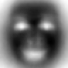
\includegraphics[interpolate=true,width=0.680000in,height=0.680000in]{weights-comparison-img0.png}}%
\end{pgfscope}%
\begin{pgfscope}%
\pgfpathrectangle{\pgfqpoint{0.881364in}{1.680588in}}{\pgfqpoint{0.679412in}{0.679412in}}%
\pgfusepath{clip}%
\pgfsys@transformshift{0.881364in}{1.680588in}%
\pgftext[left,bottom]{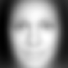
\includegraphics[interpolate=true,width=0.680000in,height=0.680000in]{weights-comparison-img1.png}}%
\end{pgfscope}%
\begin{pgfscope}%
\pgfpathrectangle{\pgfqpoint{0.050000in}{0.865294in}}{\pgfqpoint{0.679412in}{0.679412in}}%
\pgfusepath{clip}%
\pgfsys@transformshift{0.050000in}{0.865294in}%
\pgftext[left,bottom]{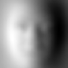
\includegraphics[interpolate=true,width=0.680000in,height=0.680000in]{weights-comparison-img2.png}}%
\end{pgfscope}%
\begin{pgfscope}%
\pgfpathrectangle{\pgfqpoint{0.881364in}{0.865294in}}{\pgfqpoint{0.679412in}{0.679412in}}%
\pgfusepath{clip}%
\pgfsys@transformshift{0.881364in}{0.865294in}%
\pgftext[left,bottom]{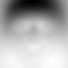
\includegraphics[interpolate=true,width=0.680000in,height=0.680000in]{weights-comparison-img3.png}}%
\end{pgfscope}%
\begin{pgfscope}%
\pgfpathrectangle{\pgfqpoint{0.050000in}{0.050000in}}{\pgfqpoint{0.679412in}{0.679412in}}%
\pgfusepath{clip}%
\pgfsys@transformshift{0.050000in}{0.050000in}%
\pgftext[left,bottom]{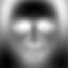
\includegraphics[interpolate=true,width=0.680000in,height=0.680000in]{weights-comparison-img4.png}}%
\end{pgfscope}%
\begin{pgfscope}%
\pgfpathrectangle{\pgfqpoint{0.881364in}{0.050000in}}{\pgfqpoint{0.679412in}{0.679412in}}%
\pgfusepath{clip}%
\pgfsys@transformshift{0.881364in}{0.050000in}%
\pgftext[left,bottom]{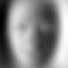
\includegraphics[interpolate=true,width=0.680000in,height=0.680000in]{weights-comparison-img5.png}}%
\end{pgfscope}%
\begin{pgfscope}%
\definecolor{textcolor}{rgb}{0.000000,0.000000,0.000000}%
\pgfsetstrokecolor{textcolor}%
\pgfsetfillcolor{textcolor}%
\pgftext[x=0.780804in,y=2.660000in,,top]{\color{textcolor}\rmfamily\fontsize{12.000000}{14.400000}\selectfont PCA}%
\end{pgfscope}%
\begin{pgfscope}%
\pgfsetbuttcap%
\pgfsetmiterjoin%
\definecolor{currentfill}{rgb}{1.000000,1.000000,1.000000}%
\pgfsetfillcolor{currentfill}%
\pgfsetlinewidth{0.000000pt}%
\definecolor{currentstroke}{rgb}{1.000000,1.000000,1.000000}%
\pgfsetstrokecolor{currentstroke}%
\pgfsetdash{}{0pt}%
\pgfpathmoveto{\pgfqpoint{1.764138in}{-0.280000in}}%
\pgfpathlineto{\pgfqpoint{3.730804in}{-0.280000in}}%
\pgfpathlineto{\pgfqpoint{3.730804in}{2.720000in}}%
\pgfpathlineto{\pgfqpoint{1.764138in}{2.720000in}}%
\pgfpathlineto{\pgfqpoint{1.764138in}{-0.280000in}}%
\pgfpathclose%
\pgfusepath{fill}%
\end{pgfscope}%
\begin{pgfscope}%
\pgfpathrectangle{\pgfqpoint{2.016667in}{1.680588in}}{\pgfqpoint{0.679412in}{0.679412in}}%
\pgfusepath{clip}%
\pgfsys@transformshift{2.016667in}{1.680588in}%
\pgftext[left,bottom]{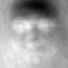
\includegraphics[interpolate=true,width=0.680000in,height=0.680000in]{weights-comparison-img6.png}}%
\end{pgfscope}%
\begin{pgfscope}%
\pgfpathrectangle{\pgfqpoint{2.848030in}{1.680588in}}{\pgfqpoint{0.679412in}{0.679412in}}%
\pgfusepath{clip}%
\pgfsys@transformshift{2.848030in}{1.680588in}%
\pgftext[left,bottom]{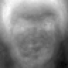
\includegraphics[interpolate=true,width=0.680000in,height=0.680000in]{weights-comparison-img7.png}}%
\end{pgfscope}%
\begin{pgfscope}%
\pgfpathrectangle{\pgfqpoint{2.016667in}{0.865294in}}{\pgfqpoint{0.679412in}{0.679412in}}%
\pgfusepath{clip}%
\pgfsys@transformshift{2.016667in}{0.865294in}%
\pgftext[left,bottom]{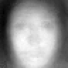
\includegraphics[interpolate=true,width=0.680000in,height=0.680000in]{weights-comparison-img8.png}}%
\end{pgfscope}%
\begin{pgfscope}%
\pgfpathrectangle{\pgfqpoint{2.848030in}{0.865294in}}{\pgfqpoint{0.679412in}{0.679412in}}%
\pgfusepath{clip}%
\pgfsys@transformshift{2.848030in}{0.865294in}%
\pgftext[left,bottom]{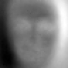
\includegraphics[interpolate=true,width=0.680000in,height=0.680000in]{weights-comparison-img9.png}}%
\end{pgfscope}%
\begin{pgfscope}%
\pgfpathrectangle{\pgfqpoint{2.016667in}{0.050000in}}{\pgfqpoint{0.679412in}{0.679412in}}%
\pgfusepath{clip}%
\pgfsys@transformshift{2.016667in}{0.050000in}%
\pgftext[left,bottom]{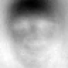
\includegraphics[interpolate=true,width=0.680000in,height=0.680000in]{weights-comparison-img10.png}}%
\end{pgfscope}%
\begin{pgfscope}%
\pgfpathrectangle{\pgfqpoint{2.848030in}{0.050000in}}{\pgfqpoint{0.679412in}{0.679412in}}%
\pgfusepath{clip}%
\pgfsys@transformshift{2.848030in}{0.050000in}%
\pgftext[left,bottom]{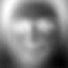
\includegraphics[interpolate=true,width=0.680000in,height=0.680000in]{weights-comparison-img11.png}}%
\end{pgfscope}%
\begin{pgfscope}%
\definecolor{textcolor}{rgb}{0.000000,0.000000,0.000000}%
\pgfsetstrokecolor{textcolor}%
\pgfsetfillcolor{textcolor}%
\pgftext[x=2.747471in,y=2.660000in,,top]{\color{textcolor}\rmfamily\fontsize{12.000000}{14.400000}\selectfont Linear AE}%
\end{pgfscope}%
\begin{pgfscope}%
\pgfsetbuttcap%
\pgfsetmiterjoin%
\definecolor{currentfill}{rgb}{1.000000,1.000000,1.000000}%
\pgfsetfillcolor{currentfill}%
\pgfsetlinewidth{0.000000pt}%
\definecolor{currentstroke}{rgb}{1.000000,1.000000,1.000000}%
\pgfsetstrokecolor{currentstroke}%
\pgfsetdash{}{0pt}%
\pgfpathmoveto{\pgfqpoint{3.730804in}{-0.280000in}}%
\pgfpathlineto{\pgfqpoint{5.697471in}{-0.280000in}}%
\pgfpathlineto{\pgfqpoint{5.697471in}{2.720000in}}%
\pgfpathlineto{\pgfqpoint{3.730804in}{2.720000in}}%
\pgfpathlineto{\pgfqpoint{3.730804in}{-0.280000in}}%
\pgfpathclose%
\pgfusepath{fill}%
\end{pgfscope}%
\begin{pgfscope}%
\pgfpathrectangle{\pgfqpoint{3.983333in}{1.680588in}}{\pgfqpoint{0.679412in}{0.679412in}}%
\pgfusepath{clip}%
\pgfsys@transformshift{3.983333in}{1.680588in}%
\pgftext[left,bottom]{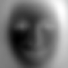
\includegraphics[interpolate=true,width=0.680000in,height=0.680000in]{weights-comparison-img12.png}}%
\end{pgfscope}%
\begin{pgfscope}%
\pgfpathrectangle{\pgfqpoint{4.814697in}{1.680588in}}{\pgfqpoint{0.679412in}{0.679412in}}%
\pgfusepath{clip}%
\pgfsys@transformshift{4.814697in}{1.680588in}%
\pgftext[left,bottom]{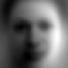
\includegraphics[interpolate=true,width=0.680000in,height=0.680000in]{weights-comparison-img13.png}}%
\end{pgfscope}%
\begin{pgfscope}%
\pgfpathrectangle{\pgfqpoint{3.983333in}{0.865294in}}{\pgfqpoint{0.679412in}{0.679412in}}%
\pgfusepath{clip}%
\pgfsys@transformshift{3.983333in}{0.865294in}%
\pgftext[left,bottom]{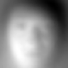
\includegraphics[interpolate=true,width=0.680000in,height=0.680000in]{weights-comparison-img14.png}}%
\end{pgfscope}%
\begin{pgfscope}%
\pgfpathrectangle{\pgfqpoint{4.814697in}{0.865294in}}{\pgfqpoint{0.679412in}{0.679412in}}%
\pgfusepath{clip}%
\pgfsys@transformshift{4.814697in}{0.865294in}%
\pgftext[left,bottom]{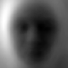
\includegraphics[interpolate=true,width=0.680000in,height=0.680000in]{weights-comparison-img15.png}}%
\end{pgfscope}%
\begin{pgfscope}%
\pgfpathrectangle{\pgfqpoint{3.983333in}{0.050000in}}{\pgfqpoint{0.679412in}{0.679412in}}%
\pgfusepath{clip}%
\pgfsys@transformshift{3.983333in}{0.050000in}%
\pgftext[left,bottom]{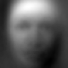
\includegraphics[interpolate=true,width=0.680000in,height=0.680000in]{weights-comparison-img16.png}}%
\end{pgfscope}%
\begin{pgfscope}%
\pgfpathrectangle{\pgfqpoint{4.814697in}{0.050000in}}{\pgfqpoint{0.679412in}{0.679412in}}%
\pgfusepath{clip}%
\pgfsys@transformshift{4.814697in}{0.050000in}%
\pgftext[left,bottom]{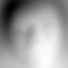
\includegraphics[interpolate=true,width=0.680000in,height=0.680000in]{weights-comparison-img17.png}}%
\end{pgfscope}%
\begin{pgfscope}%
\definecolor{textcolor}{rgb}{0.000000,0.000000,0.000000}%
\pgfsetstrokecolor{textcolor}%
\pgfsetfillcolor{textcolor}%
\pgftext[x=4.714138in,y=2.660000in,,top]{\color{textcolor}\rmfamily\fontsize{12.000000}{14.400000}\selectfont Sigmoid-linear AE}%
\end{pgfscope}%
\end{pgfpicture}%
\makeatother%
\endgroup%

	\caption[Die Gewichtsmatrizen von ausgewählten Methoden auf dem FER Datensatz]{Gezeigt sind die Gewichtsmatrizen von drei Methoden bei einer Reduktion des FER Datensatz auf sechs Dimensionen. Ein einzelnes Bild entspricht einer Spalte der Ladungs- beziehungsweise Gewichtsmatrix, welche in die Größe des Bildes umgeformt wurde. \captiona Die Ladungsmatrix $\mat{A}$ der Hauptkomponentenanalyse \captionb Die Decoder-Gewichtsmatrix eines linearen dreischichtigen Autoencoders \captionc Die Decoder-Gewichtsmatrix eines nichtlinearen dreischichtigen Autoencoders, wobei der Encoder eine Sigmoid-Aktivierungsfunktion einsetzt und der Decoder linear ist.
		Bei genauer Betrachtung der Ladungen von PCA \captiona und der Gewichte des linearen Autoencoders \captionb fällt auf, dass diese bis auf die Vorzeichen (erkennbar am invertierten Grauwert) fast identisch sind. Ist der Encoder nichtlinear wie in \captionc, so ist dies nicht mehr der Fall. (Eigene Darstellung, angelehnt an \textcite[5]{Plaut.2018})}
	\label{fig:Gewichtsvergleich}
\end{figure}
Hierbei ist in \captiona die Ladungsmatrix von PCA, in \captionb die Gewichtsmatrix $\mat{W}_2$ eines linearen dreischichtigen Autoencoders und in \captionc die Gewichtsmatrix $\mat{W}_2$ eines nichtlinearen Autoencoders dargestellt. Wie zu erkennen ist, sind
die Gewichte des linearen Autoencoders bis auf das Vorzeichen sehr ähnlich zur Ladungsmatrix von
PCA.
%% ==============================
\chapter{Schluss}
\label{sec:Schluss}
%% ==============================

\backmatter
\pagenumbering{Roman}

%% --------------------
%% |   Bibliography   |
%% --------------------

\phantomsection
\addcontentsline{toc}{chapter}{\bibname}
\begingroup
\setlength\bibitemsep{8pt}
\printbibliography
\endgroup

%% ----------------
%% |   Appendix   |
%% ----------------

\appendix
%% appendix.tex
%%

\chapter{Appendix}
\label{ch:Appendix}

\section{Autoencoder Architektur und Training Details}
\label{ch:Appendix:Architektur-Details}
In diesem Abschnitt werden Details zu den Autoencoder-Architekturen und Details zum Training der Autoencoder erläutert. Zuerst werden die Architekturen der klassischen vollvernetzten Autoencoder (AE), dann die Architekturen der Convolutional Autoencoder (ConvAE) und zuletzt die Architektur der Contractive Autoencoder (CAE) spezifiziert. Anschließend wird der benutzte Optimierer und andere Trainings-Details genannt. Da die Architekturen sehr vom Datensatz abhängen, werden diese in folgender Tabelle nach dem Datensatz gruppiert.

\ldots

Alle Autoencoder werden mit dem \textit{PyTorch}-Framework implementiert, wobei \textit{Skorch} für
die Kompatibilität mit anderen \textit{Scikit-Learn} Algorithmen eingesetzt wird. Als Optimierer
wird \textit{Adam} eingesetzt, der häufig für das Trainieren neuronaler Netze gegenüber anderen
Optimierern wie \textit{Stochastic Gradient Descent} (SGD) präferiert wird. Die Lernrate $\eta$
wird mittels eines exponentiellen Verfalls nach jeder Epoche aktualisiert. Dazu wird $\eta$ nach
jeder Epoche $t = 1, \ldots, t_{\text{max}}$ mit einem Wert $\gamma$ multipliziert. Dieser Wert
wird für alle Autoencoder auf $\gamma = 0.9$ gesetzt. Die klassischen und Contractive Autoencoder
werden für maximal 100 Epochen und die Convolutional Autoencoder für maximal 150 Epochen trainiert.
Das Training wird frühzeitig beendet, wenn sich der Validierungsfehler innerhalb von 20 Epochen
nicht mehr verbessert. Die Größes eines Batches ist datensatzabhängig gewählt worden und beträgt 32
für Swiss Roll und Twin Peaks, acht für Olivetti Faces, 100 für MNIST, 64 für LfwPeople, acht für
ICMR, und 100 für FER-2013.

\section{Qualitätskriterien für die Datensätze}
\label{ch:Appendix:Qualitaetskriterien}

In diesem Abschnitt werden die Abbildungen der Qualitätskriterien für die restlichen Datensätze
gesammelt. In \figref{fig:TwinPeaksMetrics} sind die Qualitätskriterien für die Twin Peaks, in
\figref{fig:ICMRMetrics} die Qualitätskriterien für ICMR, in \figref{fig:OlivettiFacesMetrics} die
Qualitätskriterien für den Olivetti Faces Datensatz, in \figref{fig:LfwPeopleMetrics} für den
LFW-People Datensatz und in \figref{fig:FER2013Metrics} für den FER-2013 Datensatz.
\begin{figure}[ht]
	\begin{center}
		%% Creator: Matplotlib, PGF backend
%%
%% To include the figure in your LaTeX document, write
%%   \input{<filename>.pgf}
%%
%% Make sure the required packages are loaded in your preamble
%%   \usepackage{pgf}
%%
%% Also ensure that all the required font packages are loaded; for instance,
%% the lmodern package is sometimes necessary when using math font.
%%   \usepackage{lmodern}
%%
%% Figures using additional raster images can only be included by \input if
%% they are in the same directory as the main LaTeX file. For loading figures
%% from other directories you can use the `import` package
%%   \usepackage{import}
%%
%% and then include the figures with
%%   \import{<path to file>}{<filename>.pgf}
%%
%% Matplotlib used the following preamble
%%   
%%   \usepackage{fontspec}
%%   \setmainfont{DejaVuSerif.ttf}[Path=\detokenize{/Users/moritzmistol/.pyenv/versions/3.9.13/envs/thesis/lib/python3.9/site-packages/matplotlib/mpl-data/fonts/ttf/}]
%%   \setsansfont{DejaVuSans.ttf}[Path=\detokenize{/Users/moritzmistol/.pyenv/versions/3.9.13/envs/thesis/lib/python3.9/site-packages/matplotlib/mpl-data/fonts/ttf/}]
%%   \setmonofont{DejaVuSansMono.ttf}[Path=\detokenize{/Users/moritzmistol/.pyenv/versions/3.9.13/envs/thesis/lib/python3.9/site-packages/matplotlib/mpl-data/fonts/ttf/}]
%%   \makeatletter\@ifpackageloaded{underscore}{}{\usepackage[strings]{underscore}}\makeatother
%%
\begingroup%
\makeatletter%
\begin{pgfpicture}%
\pgfpathrectangle{\pgfpointorigin}{\pgfqpoint{5.711701in}{4.634154in}}%
\pgfusepath{use as bounding box, clip}%
\begin{pgfscope}%
\pgfsetbuttcap%
\pgfsetmiterjoin%
\definecolor{currentfill}{rgb}{1.000000,1.000000,1.000000}%
\pgfsetfillcolor{currentfill}%
\pgfsetlinewidth{0.000000pt}%
\definecolor{currentstroke}{rgb}{1.000000,1.000000,1.000000}%
\pgfsetstrokecolor{currentstroke}%
\pgfsetdash{}{0pt}%
\pgfpathmoveto{\pgfqpoint{-0.000000in}{-0.000000in}}%
\pgfpathlineto{\pgfqpoint{5.711701in}{-0.000000in}}%
\pgfpathlineto{\pgfqpoint{5.711701in}{4.634154in}}%
\pgfpathlineto{\pgfqpoint{-0.000000in}{4.634154in}}%
\pgfpathlineto{\pgfqpoint{-0.000000in}{-0.000000in}}%
\pgfpathclose%
\pgfusepath{fill}%
\end{pgfscope}%
\begin{pgfscope}%
\pgfsetbuttcap%
\pgfsetmiterjoin%
\definecolor{currentfill}{rgb}{1.000000,1.000000,1.000000}%
\pgfsetfillcolor{currentfill}%
\pgfsetlinewidth{0.000000pt}%
\definecolor{currentstroke}{rgb}{0.000000,0.000000,0.000000}%
\pgfsetstrokecolor{currentstroke}%
\pgfsetstrokeopacity{0.000000}%
\pgfsetdash{}{0pt}%
\pgfpathmoveto{\pgfqpoint{0.609415in}{2.747992in}}%
\pgfpathlineto{\pgfqpoint{2.816293in}{2.747992in}}%
\pgfpathlineto{\pgfqpoint{2.816293in}{4.374193in}}%
\pgfpathlineto{\pgfqpoint{0.609415in}{4.374193in}}%
\pgfpathlineto{\pgfqpoint{0.609415in}{2.747992in}}%
\pgfpathclose%
\pgfusepath{fill}%
\end{pgfscope}%
\begin{pgfscope}%
\pgfsetbuttcap%
\pgfsetroundjoin%
\definecolor{currentfill}{rgb}{0.000000,0.000000,0.000000}%
\pgfsetfillcolor{currentfill}%
\pgfsetlinewidth{0.501875pt}%
\definecolor{currentstroke}{rgb}{0.000000,0.000000,0.000000}%
\pgfsetstrokecolor{currentstroke}%
\pgfsetdash{}{0pt}%
\pgfsys@defobject{currentmarker}{\pgfqpoint{0.000000in}{0.000000in}}{\pgfqpoint{0.000000in}{0.041667in}}{%
\pgfpathmoveto{\pgfqpoint{0.000000in}{0.000000in}}%
\pgfpathlineto{\pgfqpoint{0.000000in}{0.041667in}}%
\pgfusepath{stroke,fill}%
}%
\begin{pgfscope}%
\pgfsys@transformshift{0.609415in}{2.747992in}%
\pgfsys@useobject{currentmarker}{}%
\end{pgfscope}%
\end{pgfscope}%
\begin{pgfscope}%
\pgfsetbuttcap%
\pgfsetroundjoin%
\definecolor{currentfill}{rgb}{0.000000,0.000000,0.000000}%
\pgfsetfillcolor{currentfill}%
\pgfsetlinewidth{0.501875pt}%
\definecolor{currentstroke}{rgb}{0.000000,0.000000,0.000000}%
\pgfsetstrokecolor{currentstroke}%
\pgfsetdash{}{0pt}%
\pgfsys@defobject{currentmarker}{\pgfqpoint{0.000000in}{-0.041667in}}{\pgfqpoint{0.000000in}{0.000000in}}{%
\pgfpathmoveto{\pgfqpoint{0.000000in}{0.000000in}}%
\pgfpathlineto{\pgfqpoint{0.000000in}{-0.041667in}}%
\pgfusepath{stroke,fill}%
}%
\begin{pgfscope}%
\pgfsys@transformshift{0.609415in}{4.374193in}%
\pgfsys@useobject{currentmarker}{}%
\end{pgfscope}%
\end{pgfscope}%
\begin{pgfscope}%
\definecolor{textcolor}{rgb}{0.000000,0.000000,0.000000}%
\pgfsetstrokecolor{textcolor}%
\pgfsetfillcolor{textcolor}%
\pgftext[x=0.609415in,y=2.699381in,,top]{\color{textcolor}\rmfamily\fontsize{10.000000}{12.000000}\selectfont \(\displaystyle {0}\)}%
\end{pgfscope}%
\begin{pgfscope}%
\pgfsetbuttcap%
\pgfsetroundjoin%
\definecolor{currentfill}{rgb}{0.000000,0.000000,0.000000}%
\pgfsetfillcolor{currentfill}%
\pgfsetlinewidth{0.501875pt}%
\definecolor{currentstroke}{rgb}{0.000000,0.000000,0.000000}%
\pgfsetstrokecolor{currentstroke}%
\pgfsetdash{}{0pt}%
\pgfsys@defobject{currentmarker}{\pgfqpoint{0.000000in}{0.000000in}}{\pgfqpoint{0.000000in}{0.041667in}}{%
\pgfpathmoveto{\pgfqpoint{0.000000in}{0.000000in}}%
\pgfpathlineto{\pgfqpoint{0.000000in}{0.041667in}}%
\pgfusepath{stroke,fill}%
}%
\begin{pgfscope}%
\pgfsys@transformshift{1.046420in}{2.747992in}%
\pgfsys@useobject{currentmarker}{}%
\end{pgfscope}%
\end{pgfscope}%
\begin{pgfscope}%
\pgfsetbuttcap%
\pgfsetroundjoin%
\definecolor{currentfill}{rgb}{0.000000,0.000000,0.000000}%
\pgfsetfillcolor{currentfill}%
\pgfsetlinewidth{0.501875pt}%
\definecolor{currentstroke}{rgb}{0.000000,0.000000,0.000000}%
\pgfsetstrokecolor{currentstroke}%
\pgfsetdash{}{0pt}%
\pgfsys@defobject{currentmarker}{\pgfqpoint{0.000000in}{-0.041667in}}{\pgfqpoint{0.000000in}{0.000000in}}{%
\pgfpathmoveto{\pgfqpoint{0.000000in}{0.000000in}}%
\pgfpathlineto{\pgfqpoint{0.000000in}{-0.041667in}}%
\pgfusepath{stroke,fill}%
}%
\begin{pgfscope}%
\pgfsys@transformshift{1.046420in}{4.374193in}%
\pgfsys@useobject{currentmarker}{}%
\end{pgfscope}%
\end{pgfscope}%
\begin{pgfscope}%
\definecolor{textcolor}{rgb}{0.000000,0.000000,0.000000}%
\pgfsetstrokecolor{textcolor}%
\pgfsetfillcolor{textcolor}%
\pgftext[x=1.046420in,y=2.699381in,,top]{\color{textcolor}\rmfamily\fontsize{10.000000}{12.000000}\selectfont \(\displaystyle {20}\)}%
\end{pgfscope}%
\begin{pgfscope}%
\pgfsetbuttcap%
\pgfsetroundjoin%
\definecolor{currentfill}{rgb}{0.000000,0.000000,0.000000}%
\pgfsetfillcolor{currentfill}%
\pgfsetlinewidth{0.501875pt}%
\definecolor{currentstroke}{rgb}{0.000000,0.000000,0.000000}%
\pgfsetstrokecolor{currentstroke}%
\pgfsetdash{}{0pt}%
\pgfsys@defobject{currentmarker}{\pgfqpoint{0.000000in}{0.000000in}}{\pgfqpoint{0.000000in}{0.041667in}}{%
\pgfpathmoveto{\pgfqpoint{0.000000in}{0.000000in}}%
\pgfpathlineto{\pgfqpoint{0.000000in}{0.041667in}}%
\pgfusepath{stroke,fill}%
}%
\begin{pgfscope}%
\pgfsys@transformshift{1.483426in}{2.747992in}%
\pgfsys@useobject{currentmarker}{}%
\end{pgfscope}%
\end{pgfscope}%
\begin{pgfscope}%
\pgfsetbuttcap%
\pgfsetroundjoin%
\definecolor{currentfill}{rgb}{0.000000,0.000000,0.000000}%
\pgfsetfillcolor{currentfill}%
\pgfsetlinewidth{0.501875pt}%
\definecolor{currentstroke}{rgb}{0.000000,0.000000,0.000000}%
\pgfsetstrokecolor{currentstroke}%
\pgfsetdash{}{0pt}%
\pgfsys@defobject{currentmarker}{\pgfqpoint{0.000000in}{-0.041667in}}{\pgfqpoint{0.000000in}{0.000000in}}{%
\pgfpathmoveto{\pgfqpoint{0.000000in}{0.000000in}}%
\pgfpathlineto{\pgfqpoint{0.000000in}{-0.041667in}}%
\pgfusepath{stroke,fill}%
}%
\begin{pgfscope}%
\pgfsys@transformshift{1.483426in}{4.374193in}%
\pgfsys@useobject{currentmarker}{}%
\end{pgfscope}%
\end{pgfscope}%
\begin{pgfscope}%
\definecolor{textcolor}{rgb}{0.000000,0.000000,0.000000}%
\pgfsetstrokecolor{textcolor}%
\pgfsetfillcolor{textcolor}%
\pgftext[x=1.483426in,y=2.699381in,,top]{\color{textcolor}\rmfamily\fontsize{10.000000}{12.000000}\selectfont \(\displaystyle {40}\)}%
\end{pgfscope}%
\begin{pgfscope}%
\pgfsetbuttcap%
\pgfsetroundjoin%
\definecolor{currentfill}{rgb}{0.000000,0.000000,0.000000}%
\pgfsetfillcolor{currentfill}%
\pgfsetlinewidth{0.501875pt}%
\definecolor{currentstroke}{rgb}{0.000000,0.000000,0.000000}%
\pgfsetstrokecolor{currentstroke}%
\pgfsetdash{}{0pt}%
\pgfsys@defobject{currentmarker}{\pgfqpoint{0.000000in}{0.000000in}}{\pgfqpoint{0.000000in}{0.041667in}}{%
\pgfpathmoveto{\pgfqpoint{0.000000in}{0.000000in}}%
\pgfpathlineto{\pgfqpoint{0.000000in}{0.041667in}}%
\pgfusepath{stroke,fill}%
}%
\begin{pgfscope}%
\pgfsys@transformshift{1.920432in}{2.747992in}%
\pgfsys@useobject{currentmarker}{}%
\end{pgfscope}%
\end{pgfscope}%
\begin{pgfscope}%
\pgfsetbuttcap%
\pgfsetroundjoin%
\definecolor{currentfill}{rgb}{0.000000,0.000000,0.000000}%
\pgfsetfillcolor{currentfill}%
\pgfsetlinewidth{0.501875pt}%
\definecolor{currentstroke}{rgb}{0.000000,0.000000,0.000000}%
\pgfsetstrokecolor{currentstroke}%
\pgfsetdash{}{0pt}%
\pgfsys@defobject{currentmarker}{\pgfqpoint{0.000000in}{-0.041667in}}{\pgfqpoint{0.000000in}{0.000000in}}{%
\pgfpathmoveto{\pgfqpoint{0.000000in}{0.000000in}}%
\pgfpathlineto{\pgfqpoint{0.000000in}{-0.041667in}}%
\pgfusepath{stroke,fill}%
}%
\begin{pgfscope}%
\pgfsys@transformshift{1.920432in}{4.374193in}%
\pgfsys@useobject{currentmarker}{}%
\end{pgfscope}%
\end{pgfscope}%
\begin{pgfscope}%
\definecolor{textcolor}{rgb}{0.000000,0.000000,0.000000}%
\pgfsetstrokecolor{textcolor}%
\pgfsetfillcolor{textcolor}%
\pgftext[x=1.920432in,y=2.699381in,,top]{\color{textcolor}\rmfamily\fontsize{10.000000}{12.000000}\selectfont \(\displaystyle {60}\)}%
\end{pgfscope}%
\begin{pgfscope}%
\pgfsetbuttcap%
\pgfsetroundjoin%
\definecolor{currentfill}{rgb}{0.000000,0.000000,0.000000}%
\pgfsetfillcolor{currentfill}%
\pgfsetlinewidth{0.501875pt}%
\definecolor{currentstroke}{rgb}{0.000000,0.000000,0.000000}%
\pgfsetstrokecolor{currentstroke}%
\pgfsetdash{}{0pt}%
\pgfsys@defobject{currentmarker}{\pgfqpoint{0.000000in}{0.000000in}}{\pgfqpoint{0.000000in}{0.041667in}}{%
\pgfpathmoveto{\pgfqpoint{0.000000in}{0.000000in}}%
\pgfpathlineto{\pgfqpoint{0.000000in}{0.041667in}}%
\pgfusepath{stroke,fill}%
}%
\begin{pgfscope}%
\pgfsys@transformshift{2.357437in}{2.747992in}%
\pgfsys@useobject{currentmarker}{}%
\end{pgfscope}%
\end{pgfscope}%
\begin{pgfscope}%
\pgfsetbuttcap%
\pgfsetroundjoin%
\definecolor{currentfill}{rgb}{0.000000,0.000000,0.000000}%
\pgfsetfillcolor{currentfill}%
\pgfsetlinewidth{0.501875pt}%
\definecolor{currentstroke}{rgb}{0.000000,0.000000,0.000000}%
\pgfsetstrokecolor{currentstroke}%
\pgfsetdash{}{0pt}%
\pgfsys@defobject{currentmarker}{\pgfqpoint{0.000000in}{-0.041667in}}{\pgfqpoint{0.000000in}{0.000000in}}{%
\pgfpathmoveto{\pgfqpoint{0.000000in}{0.000000in}}%
\pgfpathlineto{\pgfqpoint{0.000000in}{-0.041667in}}%
\pgfusepath{stroke,fill}%
}%
\begin{pgfscope}%
\pgfsys@transformshift{2.357437in}{4.374193in}%
\pgfsys@useobject{currentmarker}{}%
\end{pgfscope}%
\end{pgfscope}%
\begin{pgfscope}%
\definecolor{textcolor}{rgb}{0.000000,0.000000,0.000000}%
\pgfsetstrokecolor{textcolor}%
\pgfsetfillcolor{textcolor}%
\pgftext[x=2.357437in,y=2.699381in,,top]{\color{textcolor}\rmfamily\fontsize{10.000000}{12.000000}\selectfont \(\displaystyle {80}\)}%
\end{pgfscope}%
\begin{pgfscope}%
\pgfsetbuttcap%
\pgfsetroundjoin%
\definecolor{currentfill}{rgb}{0.000000,0.000000,0.000000}%
\pgfsetfillcolor{currentfill}%
\pgfsetlinewidth{0.501875pt}%
\definecolor{currentstroke}{rgb}{0.000000,0.000000,0.000000}%
\pgfsetstrokecolor{currentstroke}%
\pgfsetdash{}{0pt}%
\pgfsys@defobject{currentmarker}{\pgfqpoint{0.000000in}{0.000000in}}{\pgfqpoint{0.000000in}{0.020833in}}{%
\pgfpathmoveto{\pgfqpoint{0.000000in}{0.000000in}}%
\pgfpathlineto{\pgfqpoint{0.000000in}{0.020833in}}%
\pgfusepath{stroke,fill}%
}%
\begin{pgfscope}%
\pgfsys@transformshift{0.718666in}{2.747992in}%
\pgfsys@useobject{currentmarker}{}%
\end{pgfscope}%
\end{pgfscope}%
\begin{pgfscope}%
\pgfsetbuttcap%
\pgfsetroundjoin%
\definecolor{currentfill}{rgb}{0.000000,0.000000,0.000000}%
\pgfsetfillcolor{currentfill}%
\pgfsetlinewidth{0.501875pt}%
\definecolor{currentstroke}{rgb}{0.000000,0.000000,0.000000}%
\pgfsetstrokecolor{currentstroke}%
\pgfsetdash{}{0pt}%
\pgfsys@defobject{currentmarker}{\pgfqpoint{0.000000in}{-0.020833in}}{\pgfqpoint{0.000000in}{0.000000in}}{%
\pgfpathmoveto{\pgfqpoint{0.000000in}{0.000000in}}%
\pgfpathlineto{\pgfqpoint{0.000000in}{-0.020833in}}%
\pgfusepath{stroke,fill}%
}%
\begin{pgfscope}%
\pgfsys@transformshift{0.718666in}{4.374193in}%
\pgfsys@useobject{currentmarker}{}%
\end{pgfscope}%
\end{pgfscope}%
\begin{pgfscope}%
\pgfsetbuttcap%
\pgfsetroundjoin%
\definecolor{currentfill}{rgb}{0.000000,0.000000,0.000000}%
\pgfsetfillcolor{currentfill}%
\pgfsetlinewidth{0.501875pt}%
\definecolor{currentstroke}{rgb}{0.000000,0.000000,0.000000}%
\pgfsetstrokecolor{currentstroke}%
\pgfsetdash{}{0pt}%
\pgfsys@defobject{currentmarker}{\pgfqpoint{0.000000in}{0.000000in}}{\pgfqpoint{0.000000in}{0.020833in}}{%
\pgfpathmoveto{\pgfqpoint{0.000000in}{0.000000in}}%
\pgfpathlineto{\pgfqpoint{0.000000in}{0.020833in}}%
\pgfusepath{stroke,fill}%
}%
\begin{pgfscope}%
\pgfsys@transformshift{0.827917in}{2.747992in}%
\pgfsys@useobject{currentmarker}{}%
\end{pgfscope}%
\end{pgfscope}%
\begin{pgfscope}%
\pgfsetbuttcap%
\pgfsetroundjoin%
\definecolor{currentfill}{rgb}{0.000000,0.000000,0.000000}%
\pgfsetfillcolor{currentfill}%
\pgfsetlinewidth{0.501875pt}%
\definecolor{currentstroke}{rgb}{0.000000,0.000000,0.000000}%
\pgfsetstrokecolor{currentstroke}%
\pgfsetdash{}{0pt}%
\pgfsys@defobject{currentmarker}{\pgfqpoint{0.000000in}{-0.020833in}}{\pgfqpoint{0.000000in}{0.000000in}}{%
\pgfpathmoveto{\pgfqpoint{0.000000in}{0.000000in}}%
\pgfpathlineto{\pgfqpoint{0.000000in}{-0.020833in}}%
\pgfusepath{stroke,fill}%
}%
\begin{pgfscope}%
\pgfsys@transformshift{0.827917in}{4.374193in}%
\pgfsys@useobject{currentmarker}{}%
\end{pgfscope}%
\end{pgfscope}%
\begin{pgfscope}%
\pgfsetbuttcap%
\pgfsetroundjoin%
\definecolor{currentfill}{rgb}{0.000000,0.000000,0.000000}%
\pgfsetfillcolor{currentfill}%
\pgfsetlinewidth{0.501875pt}%
\definecolor{currentstroke}{rgb}{0.000000,0.000000,0.000000}%
\pgfsetstrokecolor{currentstroke}%
\pgfsetdash{}{0pt}%
\pgfsys@defobject{currentmarker}{\pgfqpoint{0.000000in}{0.000000in}}{\pgfqpoint{0.000000in}{0.020833in}}{%
\pgfpathmoveto{\pgfqpoint{0.000000in}{0.000000in}}%
\pgfpathlineto{\pgfqpoint{0.000000in}{0.020833in}}%
\pgfusepath{stroke,fill}%
}%
\begin{pgfscope}%
\pgfsys@transformshift{0.937169in}{2.747992in}%
\pgfsys@useobject{currentmarker}{}%
\end{pgfscope}%
\end{pgfscope}%
\begin{pgfscope}%
\pgfsetbuttcap%
\pgfsetroundjoin%
\definecolor{currentfill}{rgb}{0.000000,0.000000,0.000000}%
\pgfsetfillcolor{currentfill}%
\pgfsetlinewidth{0.501875pt}%
\definecolor{currentstroke}{rgb}{0.000000,0.000000,0.000000}%
\pgfsetstrokecolor{currentstroke}%
\pgfsetdash{}{0pt}%
\pgfsys@defobject{currentmarker}{\pgfqpoint{0.000000in}{-0.020833in}}{\pgfqpoint{0.000000in}{0.000000in}}{%
\pgfpathmoveto{\pgfqpoint{0.000000in}{0.000000in}}%
\pgfpathlineto{\pgfqpoint{0.000000in}{-0.020833in}}%
\pgfusepath{stroke,fill}%
}%
\begin{pgfscope}%
\pgfsys@transformshift{0.937169in}{4.374193in}%
\pgfsys@useobject{currentmarker}{}%
\end{pgfscope}%
\end{pgfscope}%
\begin{pgfscope}%
\pgfsetbuttcap%
\pgfsetroundjoin%
\definecolor{currentfill}{rgb}{0.000000,0.000000,0.000000}%
\pgfsetfillcolor{currentfill}%
\pgfsetlinewidth{0.501875pt}%
\definecolor{currentstroke}{rgb}{0.000000,0.000000,0.000000}%
\pgfsetstrokecolor{currentstroke}%
\pgfsetdash{}{0pt}%
\pgfsys@defobject{currentmarker}{\pgfqpoint{0.000000in}{0.000000in}}{\pgfqpoint{0.000000in}{0.020833in}}{%
\pgfpathmoveto{\pgfqpoint{0.000000in}{0.000000in}}%
\pgfpathlineto{\pgfqpoint{0.000000in}{0.020833in}}%
\pgfusepath{stroke,fill}%
}%
\begin{pgfscope}%
\pgfsys@transformshift{1.155672in}{2.747992in}%
\pgfsys@useobject{currentmarker}{}%
\end{pgfscope}%
\end{pgfscope}%
\begin{pgfscope}%
\pgfsetbuttcap%
\pgfsetroundjoin%
\definecolor{currentfill}{rgb}{0.000000,0.000000,0.000000}%
\pgfsetfillcolor{currentfill}%
\pgfsetlinewidth{0.501875pt}%
\definecolor{currentstroke}{rgb}{0.000000,0.000000,0.000000}%
\pgfsetstrokecolor{currentstroke}%
\pgfsetdash{}{0pt}%
\pgfsys@defobject{currentmarker}{\pgfqpoint{0.000000in}{-0.020833in}}{\pgfqpoint{0.000000in}{0.000000in}}{%
\pgfpathmoveto{\pgfqpoint{0.000000in}{0.000000in}}%
\pgfpathlineto{\pgfqpoint{0.000000in}{-0.020833in}}%
\pgfusepath{stroke,fill}%
}%
\begin{pgfscope}%
\pgfsys@transformshift{1.155672in}{4.374193in}%
\pgfsys@useobject{currentmarker}{}%
\end{pgfscope}%
\end{pgfscope}%
\begin{pgfscope}%
\pgfsetbuttcap%
\pgfsetroundjoin%
\definecolor{currentfill}{rgb}{0.000000,0.000000,0.000000}%
\pgfsetfillcolor{currentfill}%
\pgfsetlinewidth{0.501875pt}%
\definecolor{currentstroke}{rgb}{0.000000,0.000000,0.000000}%
\pgfsetstrokecolor{currentstroke}%
\pgfsetdash{}{0pt}%
\pgfsys@defobject{currentmarker}{\pgfqpoint{0.000000in}{0.000000in}}{\pgfqpoint{0.000000in}{0.020833in}}{%
\pgfpathmoveto{\pgfqpoint{0.000000in}{0.000000in}}%
\pgfpathlineto{\pgfqpoint{0.000000in}{0.020833in}}%
\pgfusepath{stroke,fill}%
}%
\begin{pgfscope}%
\pgfsys@transformshift{1.264923in}{2.747992in}%
\pgfsys@useobject{currentmarker}{}%
\end{pgfscope}%
\end{pgfscope}%
\begin{pgfscope}%
\pgfsetbuttcap%
\pgfsetroundjoin%
\definecolor{currentfill}{rgb}{0.000000,0.000000,0.000000}%
\pgfsetfillcolor{currentfill}%
\pgfsetlinewidth{0.501875pt}%
\definecolor{currentstroke}{rgb}{0.000000,0.000000,0.000000}%
\pgfsetstrokecolor{currentstroke}%
\pgfsetdash{}{0pt}%
\pgfsys@defobject{currentmarker}{\pgfqpoint{0.000000in}{-0.020833in}}{\pgfqpoint{0.000000in}{0.000000in}}{%
\pgfpathmoveto{\pgfqpoint{0.000000in}{0.000000in}}%
\pgfpathlineto{\pgfqpoint{0.000000in}{-0.020833in}}%
\pgfusepath{stroke,fill}%
}%
\begin{pgfscope}%
\pgfsys@transformshift{1.264923in}{4.374193in}%
\pgfsys@useobject{currentmarker}{}%
\end{pgfscope}%
\end{pgfscope}%
\begin{pgfscope}%
\pgfsetbuttcap%
\pgfsetroundjoin%
\definecolor{currentfill}{rgb}{0.000000,0.000000,0.000000}%
\pgfsetfillcolor{currentfill}%
\pgfsetlinewidth{0.501875pt}%
\definecolor{currentstroke}{rgb}{0.000000,0.000000,0.000000}%
\pgfsetstrokecolor{currentstroke}%
\pgfsetdash{}{0pt}%
\pgfsys@defobject{currentmarker}{\pgfqpoint{0.000000in}{0.000000in}}{\pgfqpoint{0.000000in}{0.020833in}}{%
\pgfpathmoveto{\pgfqpoint{0.000000in}{0.000000in}}%
\pgfpathlineto{\pgfqpoint{0.000000in}{0.020833in}}%
\pgfusepath{stroke,fill}%
}%
\begin{pgfscope}%
\pgfsys@transformshift{1.374175in}{2.747992in}%
\pgfsys@useobject{currentmarker}{}%
\end{pgfscope}%
\end{pgfscope}%
\begin{pgfscope}%
\pgfsetbuttcap%
\pgfsetroundjoin%
\definecolor{currentfill}{rgb}{0.000000,0.000000,0.000000}%
\pgfsetfillcolor{currentfill}%
\pgfsetlinewidth{0.501875pt}%
\definecolor{currentstroke}{rgb}{0.000000,0.000000,0.000000}%
\pgfsetstrokecolor{currentstroke}%
\pgfsetdash{}{0pt}%
\pgfsys@defobject{currentmarker}{\pgfqpoint{0.000000in}{-0.020833in}}{\pgfqpoint{0.000000in}{0.000000in}}{%
\pgfpathmoveto{\pgfqpoint{0.000000in}{0.000000in}}%
\pgfpathlineto{\pgfqpoint{0.000000in}{-0.020833in}}%
\pgfusepath{stroke,fill}%
}%
\begin{pgfscope}%
\pgfsys@transformshift{1.374175in}{4.374193in}%
\pgfsys@useobject{currentmarker}{}%
\end{pgfscope}%
\end{pgfscope}%
\begin{pgfscope}%
\pgfsetbuttcap%
\pgfsetroundjoin%
\definecolor{currentfill}{rgb}{0.000000,0.000000,0.000000}%
\pgfsetfillcolor{currentfill}%
\pgfsetlinewidth{0.501875pt}%
\definecolor{currentstroke}{rgb}{0.000000,0.000000,0.000000}%
\pgfsetstrokecolor{currentstroke}%
\pgfsetdash{}{0pt}%
\pgfsys@defobject{currentmarker}{\pgfqpoint{0.000000in}{0.000000in}}{\pgfqpoint{0.000000in}{0.020833in}}{%
\pgfpathmoveto{\pgfqpoint{0.000000in}{0.000000in}}%
\pgfpathlineto{\pgfqpoint{0.000000in}{0.020833in}}%
\pgfusepath{stroke,fill}%
}%
\begin{pgfscope}%
\pgfsys@transformshift{1.592677in}{2.747992in}%
\pgfsys@useobject{currentmarker}{}%
\end{pgfscope}%
\end{pgfscope}%
\begin{pgfscope}%
\pgfsetbuttcap%
\pgfsetroundjoin%
\definecolor{currentfill}{rgb}{0.000000,0.000000,0.000000}%
\pgfsetfillcolor{currentfill}%
\pgfsetlinewidth{0.501875pt}%
\definecolor{currentstroke}{rgb}{0.000000,0.000000,0.000000}%
\pgfsetstrokecolor{currentstroke}%
\pgfsetdash{}{0pt}%
\pgfsys@defobject{currentmarker}{\pgfqpoint{0.000000in}{-0.020833in}}{\pgfqpoint{0.000000in}{0.000000in}}{%
\pgfpathmoveto{\pgfqpoint{0.000000in}{0.000000in}}%
\pgfpathlineto{\pgfqpoint{0.000000in}{-0.020833in}}%
\pgfusepath{stroke,fill}%
}%
\begin{pgfscope}%
\pgfsys@transformshift{1.592677in}{4.374193in}%
\pgfsys@useobject{currentmarker}{}%
\end{pgfscope}%
\end{pgfscope}%
\begin{pgfscope}%
\pgfsetbuttcap%
\pgfsetroundjoin%
\definecolor{currentfill}{rgb}{0.000000,0.000000,0.000000}%
\pgfsetfillcolor{currentfill}%
\pgfsetlinewidth{0.501875pt}%
\definecolor{currentstroke}{rgb}{0.000000,0.000000,0.000000}%
\pgfsetstrokecolor{currentstroke}%
\pgfsetdash{}{0pt}%
\pgfsys@defobject{currentmarker}{\pgfqpoint{0.000000in}{0.000000in}}{\pgfqpoint{0.000000in}{0.020833in}}{%
\pgfpathmoveto{\pgfqpoint{0.000000in}{0.000000in}}%
\pgfpathlineto{\pgfqpoint{0.000000in}{0.020833in}}%
\pgfusepath{stroke,fill}%
}%
\begin{pgfscope}%
\pgfsys@transformshift{1.701929in}{2.747992in}%
\pgfsys@useobject{currentmarker}{}%
\end{pgfscope}%
\end{pgfscope}%
\begin{pgfscope}%
\pgfsetbuttcap%
\pgfsetroundjoin%
\definecolor{currentfill}{rgb}{0.000000,0.000000,0.000000}%
\pgfsetfillcolor{currentfill}%
\pgfsetlinewidth{0.501875pt}%
\definecolor{currentstroke}{rgb}{0.000000,0.000000,0.000000}%
\pgfsetstrokecolor{currentstroke}%
\pgfsetdash{}{0pt}%
\pgfsys@defobject{currentmarker}{\pgfqpoint{0.000000in}{-0.020833in}}{\pgfqpoint{0.000000in}{0.000000in}}{%
\pgfpathmoveto{\pgfqpoint{0.000000in}{0.000000in}}%
\pgfpathlineto{\pgfqpoint{0.000000in}{-0.020833in}}%
\pgfusepath{stroke,fill}%
}%
\begin{pgfscope}%
\pgfsys@transformshift{1.701929in}{4.374193in}%
\pgfsys@useobject{currentmarker}{}%
\end{pgfscope}%
\end{pgfscope}%
\begin{pgfscope}%
\pgfsetbuttcap%
\pgfsetroundjoin%
\definecolor{currentfill}{rgb}{0.000000,0.000000,0.000000}%
\pgfsetfillcolor{currentfill}%
\pgfsetlinewidth{0.501875pt}%
\definecolor{currentstroke}{rgb}{0.000000,0.000000,0.000000}%
\pgfsetstrokecolor{currentstroke}%
\pgfsetdash{}{0pt}%
\pgfsys@defobject{currentmarker}{\pgfqpoint{0.000000in}{0.000000in}}{\pgfqpoint{0.000000in}{0.020833in}}{%
\pgfpathmoveto{\pgfqpoint{0.000000in}{0.000000in}}%
\pgfpathlineto{\pgfqpoint{0.000000in}{0.020833in}}%
\pgfusepath{stroke,fill}%
}%
\begin{pgfscope}%
\pgfsys@transformshift{1.811180in}{2.747992in}%
\pgfsys@useobject{currentmarker}{}%
\end{pgfscope}%
\end{pgfscope}%
\begin{pgfscope}%
\pgfsetbuttcap%
\pgfsetroundjoin%
\definecolor{currentfill}{rgb}{0.000000,0.000000,0.000000}%
\pgfsetfillcolor{currentfill}%
\pgfsetlinewidth{0.501875pt}%
\definecolor{currentstroke}{rgb}{0.000000,0.000000,0.000000}%
\pgfsetstrokecolor{currentstroke}%
\pgfsetdash{}{0pt}%
\pgfsys@defobject{currentmarker}{\pgfqpoint{0.000000in}{-0.020833in}}{\pgfqpoint{0.000000in}{0.000000in}}{%
\pgfpathmoveto{\pgfqpoint{0.000000in}{0.000000in}}%
\pgfpathlineto{\pgfqpoint{0.000000in}{-0.020833in}}%
\pgfusepath{stroke,fill}%
}%
\begin{pgfscope}%
\pgfsys@transformshift{1.811180in}{4.374193in}%
\pgfsys@useobject{currentmarker}{}%
\end{pgfscope}%
\end{pgfscope}%
\begin{pgfscope}%
\pgfsetbuttcap%
\pgfsetroundjoin%
\definecolor{currentfill}{rgb}{0.000000,0.000000,0.000000}%
\pgfsetfillcolor{currentfill}%
\pgfsetlinewidth{0.501875pt}%
\definecolor{currentstroke}{rgb}{0.000000,0.000000,0.000000}%
\pgfsetstrokecolor{currentstroke}%
\pgfsetdash{}{0pt}%
\pgfsys@defobject{currentmarker}{\pgfqpoint{0.000000in}{0.000000in}}{\pgfqpoint{0.000000in}{0.020833in}}{%
\pgfpathmoveto{\pgfqpoint{0.000000in}{0.000000in}}%
\pgfpathlineto{\pgfqpoint{0.000000in}{0.020833in}}%
\pgfusepath{stroke,fill}%
}%
\begin{pgfscope}%
\pgfsys@transformshift{2.029683in}{2.747992in}%
\pgfsys@useobject{currentmarker}{}%
\end{pgfscope}%
\end{pgfscope}%
\begin{pgfscope}%
\pgfsetbuttcap%
\pgfsetroundjoin%
\definecolor{currentfill}{rgb}{0.000000,0.000000,0.000000}%
\pgfsetfillcolor{currentfill}%
\pgfsetlinewidth{0.501875pt}%
\definecolor{currentstroke}{rgb}{0.000000,0.000000,0.000000}%
\pgfsetstrokecolor{currentstroke}%
\pgfsetdash{}{0pt}%
\pgfsys@defobject{currentmarker}{\pgfqpoint{0.000000in}{-0.020833in}}{\pgfqpoint{0.000000in}{0.000000in}}{%
\pgfpathmoveto{\pgfqpoint{0.000000in}{0.000000in}}%
\pgfpathlineto{\pgfqpoint{0.000000in}{-0.020833in}}%
\pgfusepath{stroke,fill}%
}%
\begin{pgfscope}%
\pgfsys@transformshift{2.029683in}{4.374193in}%
\pgfsys@useobject{currentmarker}{}%
\end{pgfscope}%
\end{pgfscope}%
\begin{pgfscope}%
\pgfsetbuttcap%
\pgfsetroundjoin%
\definecolor{currentfill}{rgb}{0.000000,0.000000,0.000000}%
\pgfsetfillcolor{currentfill}%
\pgfsetlinewidth{0.501875pt}%
\definecolor{currentstroke}{rgb}{0.000000,0.000000,0.000000}%
\pgfsetstrokecolor{currentstroke}%
\pgfsetdash{}{0pt}%
\pgfsys@defobject{currentmarker}{\pgfqpoint{0.000000in}{0.000000in}}{\pgfqpoint{0.000000in}{0.020833in}}{%
\pgfpathmoveto{\pgfqpoint{0.000000in}{0.000000in}}%
\pgfpathlineto{\pgfqpoint{0.000000in}{0.020833in}}%
\pgfusepath{stroke,fill}%
}%
\begin{pgfscope}%
\pgfsys@transformshift{2.138935in}{2.747992in}%
\pgfsys@useobject{currentmarker}{}%
\end{pgfscope}%
\end{pgfscope}%
\begin{pgfscope}%
\pgfsetbuttcap%
\pgfsetroundjoin%
\definecolor{currentfill}{rgb}{0.000000,0.000000,0.000000}%
\pgfsetfillcolor{currentfill}%
\pgfsetlinewidth{0.501875pt}%
\definecolor{currentstroke}{rgb}{0.000000,0.000000,0.000000}%
\pgfsetstrokecolor{currentstroke}%
\pgfsetdash{}{0pt}%
\pgfsys@defobject{currentmarker}{\pgfqpoint{0.000000in}{-0.020833in}}{\pgfqpoint{0.000000in}{0.000000in}}{%
\pgfpathmoveto{\pgfqpoint{0.000000in}{0.000000in}}%
\pgfpathlineto{\pgfqpoint{0.000000in}{-0.020833in}}%
\pgfusepath{stroke,fill}%
}%
\begin{pgfscope}%
\pgfsys@transformshift{2.138935in}{4.374193in}%
\pgfsys@useobject{currentmarker}{}%
\end{pgfscope}%
\end{pgfscope}%
\begin{pgfscope}%
\pgfsetbuttcap%
\pgfsetroundjoin%
\definecolor{currentfill}{rgb}{0.000000,0.000000,0.000000}%
\pgfsetfillcolor{currentfill}%
\pgfsetlinewidth{0.501875pt}%
\definecolor{currentstroke}{rgb}{0.000000,0.000000,0.000000}%
\pgfsetstrokecolor{currentstroke}%
\pgfsetdash{}{0pt}%
\pgfsys@defobject{currentmarker}{\pgfqpoint{0.000000in}{0.000000in}}{\pgfqpoint{0.000000in}{0.020833in}}{%
\pgfpathmoveto{\pgfqpoint{0.000000in}{0.000000in}}%
\pgfpathlineto{\pgfqpoint{0.000000in}{0.020833in}}%
\pgfusepath{stroke,fill}%
}%
\begin{pgfscope}%
\pgfsys@transformshift{2.248186in}{2.747992in}%
\pgfsys@useobject{currentmarker}{}%
\end{pgfscope}%
\end{pgfscope}%
\begin{pgfscope}%
\pgfsetbuttcap%
\pgfsetroundjoin%
\definecolor{currentfill}{rgb}{0.000000,0.000000,0.000000}%
\pgfsetfillcolor{currentfill}%
\pgfsetlinewidth{0.501875pt}%
\definecolor{currentstroke}{rgb}{0.000000,0.000000,0.000000}%
\pgfsetstrokecolor{currentstroke}%
\pgfsetdash{}{0pt}%
\pgfsys@defobject{currentmarker}{\pgfqpoint{0.000000in}{-0.020833in}}{\pgfqpoint{0.000000in}{0.000000in}}{%
\pgfpathmoveto{\pgfqpoint{0.000000in}{0.000000in}}%
\pgfpathlineto{\pgfqpoint{0.000000in}{-0.020833in}}%
\pgfusepath{stroke,fill}%
}%
\begin{pgfscope}%
\pgfsys@transformshift{2.248186in}{4.374193in}%
\pgfsys@useobject{currentmarker}{}%
\end{pgfscope}%
\end{pgfscope}%
\begin{pgfscope}%
\pgfsetbuttcap%
\pgfsetroundjoin%
\definecolor{currentfill}{rgb}{0.000000,0.000000,0.000000}%
\pgfsetfillcolor{currentfill}%
\pgfsetlinewidth{0.501875pt}%
\definecolor{currentstroke}{rgb}{0.000000,0.000000,0.000000}%
\pgfsetstrokecolor{currentstroke}%
\pgfsetdash{}{0pt}%
\pgfsys@defobject{currentmarker}{\pgfqpoint{0.000000in}{0.000000in}}{\pgfqpoint{0.000000in}{0.020833in}}{%
\pgfpathmoveto{\pgfqpoint{0.000000in}{0.000000in}}%
\pgfpathlineto{\pgfqpoint{0.000000in}{0.020833in}}%
\pgfusepath{stroke,fill}%
}%
\begin{pgfscope}%
\pgfsys@transformshift{2.466689in}{2.747992in}%
\pgfsys@useobject{currentmarker}{}%
\end{pgfscope}%
\end{pgfscope}%
\begin{pgfscope}%
\pgfsetbuttcap%
\pgfsetroundjoin%
\definecolor{currentfill}{rgb}{0.000000,0.000000,0.000000}%
\pgfsetfillcolor{currentfill}%
\pgfsetlinewidth{0.501875pt}%
\definecolor{currentstroke}{rgb}{0.000000,0.000000,0.000000}%
\pgfsetstrokecolor{currentstroke}%
\pgfsetdash{}{0pt}%
\pgfsys@defobject{currentmarker}{\pgfqpoint{0.000000in}{-0.020833in}}{\pgfqpoint{0.000000in}{0.000000in}}{%
\pgfpathmoveto{\pgfqpoint{0.000000in}{0.000000in}}%
\pgfpathlineto{\pgfqpoint{0.000000in}{-0.020833in}}%
\pgfusepath{stroke,fill}%
}%
\begin{pgfscope}%
\pgfsys@transformshift{2.466689in}{4.374193in}%
\pgfsys@useobject{currentmarker}{}%
\end{pgfscope}%
\end{pgfscope}%
\begin{pgfscope}%
\pgfsetbuttcap%
\pgfsetroundjoin%
\definecolor{currentfill}{rgb}{0.000000,0.000000,0.000000}%
\pgfsetfillcolor{currentfill}%
\pgfsetlinewidth{0.501875pt}%
\definecolor{currentstroke}{rgb}{0.000000,0.000000,0.000000}%
\pgfsetstrokecolor{currentstroke}%
\pgfsetdash{}{0pt}%
\pgfsys@defobject{currentmarker}{\pgfqpoint{0.000000in}{0.000000in}}{\pgfqpoint{0.000000in}{0.020833in}}{%
\pgfpathmoveto{\pgfqpoint{0.000000in}{0.000000in}}%
\pgfpathlineto{\pgfqpoint{0.000000in}{0.020833in}}%
\pgfusepath{stroke,fill}%
}%
\begin{pgfscope}%
\pgfsys@transformshift{2.575940in}{2.747992in}%
\pgfsys@useobject{currentmarker}{}%
\end{pgfscope}%
\end{pgfscope}%
\begin{pgfscope}%
\pgfsetbuttcap%
\pgfsetroundjoin%
\definecolor{currentfill}{rgb}{0.000000,0.000000,0.000000}%
\pgfsetfillcolor{currentfill}%
\pgfsetlinewidth{0.501875pt}%
\definecolor{currentstroke}{rgb}{0.000000,0.000000,0.000000}%
\pgfsetstrokecolor{currentstroke}%
\pgfsetdash{}{0pt}%
\pgfsys@defobject{currentmarker}{\pgfqpoint{0.000000in}{-0.020833in}}{\pgfqpoint{0.000000in}{0.000000in}}{%
\pgfpathmoveto{\pgfqpoint{0.000000in}{0.000000in}}%
\pgfpathlineto{\pgfqpoint{0.000000in}{-0.020833in}}%
\pgfusepath{stroke,fill}%
}%
\begin{pgfscope}%
\pgfsys@transformshift{2.575940in}{4.374193in}%
\pgfsys@useobject{currentmarker}{}%
\end{pgfscope}%
\end{pgfscope}%
\begin{pgfscope}%
\pgfsetbuttcap%
\pgfsetroundjoin%
\definecolor{currentfill}{rgb}{0.000000,0.000000,0.000000}%
\pgfsetfillcolor{currentfill}%
\pgfsetlinewidth{0.501875pt}%
\definecolor{currentstroke}{rgb}{0.000000,0.000000,0.000000}%
\pgfsetstrokecolor{currentstroke}%
\pgfsetdash{}{0pt}%
\pgfsys@defobject{currentmarker}{\pgfqpoint{0.000000in}{0.000000in}}{\pgfqpoint{0.000000in}{0.020833in}}{%
\pgfpathmoveto{\pgfqpoint{0.000000in}{0.000000in}}%
\pgfpathlineto{\pgfqpoint{0.000000in}{0.020833in}}%
\pgfusepath{stroke,fill}%
}%
\begin{pgfscope}%
\pgfsys@transformshift{2.685192in}{2.747992in}%
\pgfsys@useobject{currentmarker}{}%
\end{pgfscope}%
\end{pgfscope}%
\begin{pgfscope}%
\pgfsetbuttcap%
\pgfsetroundjoin%
\definecolor{currentfill}{rgb}{0.000000,0.000000,0.000000}%
\pgfsetfillcolor{currentfill}%
\pgfsetlinewidth{0.501875pt}%
\definecolor{currentstroke}{rgb}{0.000000,0.000000,0.000000}%
\pgfsetstrokecolor{currentstroke}%
\pgfsetdash{}{0pt}%
\pgfsys@defobject{currentmarker}{\pgfqpoint{0.000000in}{-0.020833in}}{\pgfqpoint{0.000000in}{0.000000in}}{%
\pgfpathmoveto{\pgfqpoint{0.000000in}{0.000000in}}%
\pgfpathlineto{\pgfqpoint{0.000000in}{-0.020833in}}%
\pgfusepath{stroke,fill}%
}%
\begin{pgfscope}%
\pgfsys@transformshift{2.685192in}{4.374193in}%
\pgfsys@useobject{currentmarker}{}%
\end{pgfscope}%
\end{pgfscope}%
\begin{pgfscope}%
\pgfsetbuttcap%
\pgfsetroundjoin%
\definecolor{currentfill}{rgb}{0.000000,0.000000,0.000000}%
\pgfsetfillcolor{currentfill}%
\pgfsetlinewidth{0.501875pt}%
\definecolor{currentstroke}{rgb}{0.000000,0.000000,0.000000}%
\pgfsetstrokecolor{currentstroke}%
\pgfsetdash{}{0pt}%
\pgfsys@defobject{currentmarker}{\pgfqpoint{0.000000in}{0.000000in}}{\pgfqpoint{0.000000in}{0.020833in}}{%
\pgfpathmoveto{\pgfqpoint{0.000000in}{0.000000in}}%
\pgfpathlineto{\pgfqpoint{0.000000in}{0.020833in}}%
\pgfusepath{stroke,fill}%
}%
\begin{pgfscope}%
\pgfsys@transformshift{2.794443in}{2.747992in}%
\pgfsys@useobject{currentmarker}{}%
\end{pgfscope}%
\end{pgfscope}%
\begin{pgfscope}%
\pgfsetbuttcap%
\pgfsetroundjoin%
\definecolor{currentfill}{rgb}{0.000000,0.000000,0.000000}%
\pgfsetfillcolor{currentfill}%
\pgfsetlinewidth{0.501875pt}%
\definecolor{currentstroke}{rgb}{0.000000,0.000000,0.000000}%
\pgfsetstrokecolor{currentstroke}%
\pgfsetdash{}{0pt}%
\pgfsys@defobject{currentmarker}{\pgfqpoint{0.000000in}{-0.020833in}}{\pgfqpoint{0.000000in}{0.000000in}}{%
\pgfpathmoveto{\pgfqpoint{0.000000in}{0.000000in}}%
\pgfpathlineto{\pgfqpoint{0.000000in}{-0.020833in}}%
\pgfusepath{stroke,fill}%
}%
\begin{pgfscope}%
\pgfsys@transformshift{2.794443in}{4.374193in}%
\pgfsys@useobject{currentmarker}{}%
\end{pgfscope}%
\end{pgfscope}%
\begin{pgfscope}%
\definecolor{textcolor}{rgb}{0.000000,0.000000,0.000000}%
\pgfsetstrokecolor{textcolor}%
\pgfsetfillcolor{textcolor}%
\pgftext[x=1.712854in,y=2.509413in,,top]{\color{textcolor}\rmfamily\fontsize{10.000000}{12.000000}\selectfont \(\displaystyle K\)}%
\end{pgfscope}%
\begin{pgfscope}%
\pgfsetbuttcap%
\pgfsetroundjoin%
\definecolor{currentfill}{rgb}{0.000000,0.000000,0.000000}%
\pgfsetfillcolor{currentfill}%
\pgfsetlinewidth{0.501875pt}%
\definecolor{currentstroke}{rgb}{0.000000,0.000000,0.000000}%
\pgfsetstrokecolor{currentstroke}%
\pgfsetdash{}{0pt}%
\pgfsys@defobject{currentmarker}{\pgfqpoint{0.000000in}{0.000000in}}{\pgfqpoint{0.041667in}{0.000000in}}{%
\pgfpathmoveto{\pgfqpoint{0.000000in}{0.000000in}}%
\pgfpathlineto{\pgfqpoint{0.041667in}{0.000000in}}%
\pgfusepath{stroke,fill}%
}%
\begin{pgfscope}%
\pgfsys@transformshift{0.609415in}{3.162442in}%
\pgfsys@useobject{currentmarker}{}%
\end{pgfscope}%
\end{pgfscope}%
\begin{pgfscope}%
\pgfsetbuttcap%
\pgfsetroundjoin%
\definecolor{currentfill}{rgb}{0.000000,0.000000,0.000000}%
\pgfsetfillcolor{currentfill}%
\pgfsetlinewidth{0.501875pt}%
\definecolor{currentstroke}{rgb}{0.000000,0.000000,0.000000}%
\pgfsetstrokecolor{currentstroke}%
\pgfsetdash{}{0pt}%
\pgfsys@defobject{currentmarker}{\pgfqpoint{-0.041667in}{0.000000in}}{\pgfqpoint{-0.000000in}{0.000000in}}{%
\pgfpathmoveto{\pgfqpoint{-0.000000in}{0.000000in}}%
\pgfpathlineto{\pgfqpoint{-0.041667in}{0.000000in}}%
\pgfusepath{stroke,fill}%
}%
\begin{pgfscope}%
\pgfsys@transformshift{2.816293in}{3.162442in}%
\pgfsys@useobject{currentmarker}{}%
\end{pgfscope}%
\end{pgfscope}%
\begin{pgfscope}%
\definecolor{textcolor}{rgb}{0.000000,0.000000,0.000000}%
\pgfsetstrokecolor{textcolor}%
\pgfsetfillcolor{textcolor}%
\pgftext[x=0.313889in, y=3.109681in, left, base]{\color{textcolor}\rmfamily\fontsize{10.000000}{12.000000}\selectfont \(\displaystyle {0.90}\)}%
\end{pgfscope}%
\begin{pgfscope}%
\pgfsetbuttcap%
\pgfsetroundjoin%
\definecolor{currentfill}{rgb}{0.000000,0.000000,0.000000}%
\pgfsetfillcolor{currentfill}%
\pgfsetlinewidth{0.501875pt}%
\definecolor{currentstroke}{rgb}{0.000000,0.000000,0.000000}%
\pgfsetstrokecolor{currentstroke}%
\pgfsetdash{}{0pt}%
\pgfsys@defobject{currentmarker}{\pgfqpoint{0.000000in}{0.000000in}}{\pgfqpoint{0.041667in}{0.000000in}}{%
\pgfpathmoveto{\pgfqpoint{0.000000in}{0.000000in}}%
\pgfpathlineto{\pgfqpoint{0.041667in}{0.000000in}}%
\pgfusepath{stroke,fill}%
}%
\begin{pgfscope}%
\pgfsys@transformshift{0.609415in}{3.751202in}%
\pgfsys@useobject{currentmarker}{}%
\end{pgfscope}%
\end{pgfscope}%
\begin{pgfscope}%
\pgfsetbuttcap%
\pgfsetroundjoin%
\definecolor{currentfill}{rgb}{0.000000,0.000000,0.000000}%
\pgfsetfillcolor{currentfill}%
\pgfsetlinewidth{0.501875pt}%
\definecolor{currentstroke}{rgb}{0.000000,0.000000,0.000000}%
\pgfsetstrokecolor{currentstroke}%
\pgfsetdash{}{0pt}%
\pgfsys@defobject{currentmarker}{\pgfqpoint{-0.041667in}{0.000000in}}{\pgfqpoint{-0.000000in}{0.000000in}}{%
\pgfpathmoveto{\pgfqpoint{-0.000000in}{0.000000in}}%
\pgfpathlineto{\pgfqpoint{-0.041667in}{0.000000in}}%
\pgfusepath{stroke,fill}%
}%
\begin{pgfscope}%
\pgfsys@transformshift{2.816293in}{3.751202in}%
\pgfsys@useobject{currentmarker}{}%
\end{pgfscope}%
\end{pgfscope}%
\begin{pgfscope}%
\definecolor{textcolor}{rgb}{0.000000,0.000000,0.000000}%
\pgfsetstrokecolor{textcolor}%
\pgfsetfillcolor{textcolor}%
\pgftext[x=0.313889in, y=3.698440in, left, base]{\color{textcolor}\rmfamily\fontsize{10.000000}{12.000000}\selectfont \(\displaystyle {0.95}\)}%
\end{pgfscope}%
\begin{pgfscope}%
\pgfsetbuttcap%
\pgfsetroundjoin%
\definecolor{currentfill}{rgb}{0.000000,0.000000,0.000000}%
\pgfsetfillcolor{currentfill}%
\pgfsetlinewidth{0.501875pt}%
\definecolor{currentstroke}{rgb}{0.000000,0.000000,0.000000}%
\pgfsetstrokecolor{currentstroke}%
\pgfsetdash{}{0pt}%
\pgfsys@defobject{currentmarker}{\pgfqpoint{0.000000in}{0.000000in}}{\pgfqpoint{0.041667in}{0.000000in}}{%
\pgfpathmoveto{\pgfqpoint{0.000000in}{0.000000in}}%
\pgfpathlineto{\pgfqpoint{0.041667in}{0.000000in}}%
\pgfusepath{stroke,fill}%
}%
\begin{pgfscope}%
\pgfsys@transformshift{0.609415in}{4.339962in}%
\pgfsys@useobject{currentmarker}{}%
\end{pgfscope}%
\end{pgfscope}%
\begin{pgfscope}%
\pgfsetbuttcap%
\pgfsetroundjoin%
\definecolor{currentfill}{rgb}{0.000000,0.000000,0.000000}%
\pgfsetfillcolor{currentfill}%
\pgfsetlinewidth{0.501875pt}%
\definecolor{currentstroke}{rgb}{0.000000,0.000000,0.000000}%
\pgfsetstrokecolor{currentstroke}%
\pgfsetdash{}{0pt}%
\pgfsys@defobject{currentmarker}{\pgfqpoint{-0.041667in}{0.000000in}}{\pgfqpoint{-0.000000in}{0.000000in}}{%
\pgfpathmoveto{\pgfqpoint{-0.000000in}{0.000000in}}%
\pgfpathlineto{\pgfqpoint{-0.041667in}{0.000000in}}%
\pgfusepath{stroke,fill}%
}%
\begin{pgfscope}%
\pgfsys@transformshift{2.816293in}{4.339962in}%
\pgfsys@useobject{currentmarker}{}%
\end{pgfscope}%
\end{pgfscope}%
\begin{pgfscope}%
\definecolor{textcolor}{rgb}{0.000000,0.000000,0.000000}%
\pgfsetstrokecolor{textcolor}%
\pgfsetfillcolor{textcolor}%
\pgftext[x=0.313889in, y=4.287200in, left, base]{\color{textcolor}\rmfamily\fontsize{10.000000}{12.000000}\selectfont \(\displaystyle {1.00}\)}%
\end{pgfscope}%
\begin{pgfscope}%
\pgfsetbuttcap%
\pgfsetroundjoin%
\definecolor{currentfill}{rgb}{0.000000,0.000000,0.000000}%
\pgfsetfillcolor{currentfill}%
\pgfsetlinewidth{0.501875pt}%
\definecolor{currentstroke}{rgb}{0.000000,0.000000,0.000000}%
\pgfsetstrokecolor{currentstroke}%
\pgfsetdash{}{0pt}%
\pgfsys@defobject{currentmarker}{\pgfqpoint{0.000000in}{0.000000in}}{\pgfqpoint{0.020833in}{0.000000in}}{%
\pgfpathmoveto{\pgfqpoint{0.000000in}{0.000000in}}%
\pgfpathlineto{\pgfqpoint{0.020833in}{0.000000in}}%
\pgfusepath{stroke,fill}%
}%
\begin{pgfscope}%
\pgfsys@transformshift{0.609415in}{2.809187in}%
\pgfsys@useobject{currentmarker}{}%
\end{pgfscope}%
\end{pgfscope}%
\begin{pgfscope}%
\pgfsetbuttcap%
\pgfsetroundjoin%
\definecolor{currentfill}{rgb}{0.000000,0.000000,0.000000}%
\pgfsetfillcolor{currentfill}%
\pgfsetlinewidth{0.501875pt}%
\definecolor{currentstroke}{rgb}{0.000000,0.000000,0.000000}%
\pgfsetstrokecolor{currentstroke}%
\pgfsetdash{}{0pt}%
\pgfsys@defobject{currentmarker}{\pgfqpoint{-0.020833in}{0.000000in}}{\pgfqpoint{-0.000000in}{0.000000in}}{%
\pgfpathmoveto{\pgfqpoint{-0.000000in}{0.000000in}}%
\pgfpathlineto{\pgfqpoint{-0.020833in}{0.000000in}}%
\pgfusepath{stroke,fill}%
}%
\begin{pgfscope}%
\pgfsys@transformshift{2.816293in}{2.809187in}%
\pgfsys@useobject{currentmarker}{}%
\end{pgfscope}%
\end{pgfscope}%
\begin{pgfscope}%
\pgfsetbuttcap%
\pgfsetroundjoin%
\definecolor{currentfill}{rgb}{0.000000,0.000000,0.000000}%
\pgfsetfillcolor{currentfill}%
\pgfsetlinewidth{0.501875pt}%
\definecolor{currentstroke}{rgb}{0.000000,0.000000,0.000000}%
\pgfsetstrokecolor{currentstroke}%
\pgfsetdash{}{0pt}%
\pgfsys@defobject{currentmarker}{\pgfqpoint{0.000000in}{0.000000in}}{\pgfqpoint{0.020833in}{0.000000in}}{%
\pgfpathmoveto{\pgfqpoint{0.000000in}{0.000000in}}%
\pgfpathlineto{\pgfqpoint{0.020833in}{0.000000in}}%
\pgfusepath{stroke,fill}%
}%
\begin{pgfscope}%
\pgfsys@transformshift{0.609415in}{2.926939in}%
\pgfsys@useobject{currentmarker}{}%
\end{pgfscope}%
\end{pgfscope}%
\begin{pgfscope}%
\pgfsetbuttcap%
\pgfsetroundjoin%
\definecolor{currentfill}{rgb}{0.000000,0.000000,0.000000}%
\pgfsetfillcolor{currentfill}%
\pgfsetlinewidth{0.501875pt}%
\definecolor{currentstroke}{rgb}{0.000000,0.000000,0.000000}%
\pgfsetstrokecolor{currentstroke}%
\pgfsetdash{}{0pt}%
\pgfsys@defobject{currentmarker}{\pgfqpoint{-0.020833in}{0.000000in}}{\pgfqpoint{-0.000000in}{0.000000in}}{%
\pgfpathmoveto{\pgfqpoint{-0.000000in}{0.000000in}}%
\pgfpathlineto{\pgfqpoint{-0.020833in}{0.000000in}}%
\pgfusepath{stroke,fill}%
}%
\begin{pgfscope}%
\pgfsys@transformshift{2.816293in}{2.926939in}%
\pgfsys@useobject{currentmarker}{}%
\end{pgfscope}%
\end{pgfscope}%
\begin{pgfscope}%
\pgfsetbuttcap%
\pgfsetroundjoin%
\definecolor{currentfill}{rgb}{0.000000,0.000000,0.000000}%
\pgfsetfillcolor{currentfill}%
\pgfsetlinewidth{0.501875pt}%
\definecolor{currentstroke}{rgb}{0.000000,0.000000,0.000000}%
\pgfsetstrokecolor{currentstroke}%
\pgfsetdash{}{0pt}%
\pgfsys@defobject{currentmarker}{\pgfqpoint{0.000000in}{0.000000in}}{\pgfqpoint{0.020833in}{0.000000in}}{%
\pgfpathmoveto{\pgfqpoint{0.000000in}{0.000000in}}%
\pgfpathlineto{\pgfqpoint{0.020833in}{0.000000in}}%
\pgfusepath{stroke,fill}%
}%
\begin{pgfscope}%
\pgfsys@transformshift{0.609415in}{3.044691in}%
\pgfsys@useobject{currentmarker}{}%
\end{pgfscope}%
\end{pgfscope}%
\begin{pgfscope}%
\pgfsetbuttcap%
\pgfsetroundjoin%
\definecolor{currentfill}{rgb}{0.000000,0.000000,0.000000}%
\pgfsetfillcolor{currentfill}%
\pgfsetlinewidth{0.501875pt}%
\definecolor{currentstroke}{rgb}{0.000000,0.000000,0.000000}%
\pgfsetstrokecolor{currentstroke}%
\pgfsetdash{}{0pt}%
\pgfsys@defobject{currentmarker}{\pgfqpoint{-0.020833in}{0.000000in}}{\pgfqpoint{-0.000000in}{0.000000in}}{%
\pgfpathmoveto{\pgfqpoint{-0.000000in}{0.000000in}}%
\pgfpathlineto{\pgfqpoint{-0.020833in}{0.000000in}}%
\pgfusepath{stroke,fill}%
}%
\begin{pgfscope}%
\pgfsys@transformshift{2.816293in}{3.044691in}%
\pgfsys@useobject{currentmarker}{}%
\end{pgfscope}%
\end{pgfscope}%
\begin{pgfscope}%
\pgfsetbuttcap%
\pgfsetroundjoin%
\definecolor{currentfill}{rgb}{0.000000,0.000000,0.000000}%
\pgfsetfillcolor{currentfill}%
\pgfsetlinewidth{0.501875pt}%
\definecolor{currentstroke}{rgb}{0.000000,0.000000,0.000000}%
\pgfsetstrokecolor{currentstroke}%
\pgfsetdash{}{0pt}%
\pgfsys@defobject{currentmarker}{\pgfqpoint{0.000000in}{0.000000in}}{\pgfqpoint{0.020833in}{0.000000in}}{%
\pgfpathmoveto{\pgfqpoint{0.000000in}{0.000000in}}%
\pgfpathlineto{\pgfqpoint{0.020833in}{0.000000in}}%
\pgfusepath{stroke,fill}%
}%
\begin{pgfscope}%
\pgfsys@transformshift{0.609415in}{3.280194in}%
\pgfsys@useobject{currentmarker}{}%
\end{pgfscope}%
\end{pgfscope}%
\begin{pgfscope}%
\pgfsetbuttcap%
\pgfsetroundjoin%
\definecolor{currentfill}{rgb}{0.000000,0.000000,0.000000}%
\pgfsetfillcolor{currentfill}%
\pgfsetlinewidth{0.501875pt}%
\definecolor{currentstroke}{rgb}{0.000000,0.000000,0.000000}%
\pgfsetstrokecolor{currentstroke}%
\pgfsetdash{}{0pt}%
\pgfsys@defobject{currentmarker}{\pgfqpoint{-0.020833in}{0.000000in}}{\pgfqpoint{-0.000000in}{0.000000in}}{%
\pgfpathmoveto{\pgfqpoint{-0.000000in}{0.000000in}}%
\pgfpathlineto{\pgfqpoint{-0.020833in}{0.000000in}}%
\pgfusepath{stroke,fill}%
}%
\begin{pgfscope}%
\pgfsys@transformshift{2.816293in}{3.280194in}%
\pgfsys@useobject{currentmarker}{}%
\end{pgfscope}%
\end{pgfscope}%
\begin{pgfscope}%
\pgfsetbuttcap%
\pgfsetroundjoin%
\definecolor{currentfill}{rgb}{0.000000,0.000000,0.000000}%
\pgfsetfillcolor{currentfill}%
\pgfsetlinewidth{0.501875pt}%
\definecolor{currentstroke}{rgb}{0.000000,0.000000,0.000000}%
\pgfsetstrokecolor{currentstroke}%
\pgfsetdash{}{0pt}%
\pgfsys@defobject{currentmarker}{\pgfqpoint{0.000000in}{0.000000in}}{\pgfqpoint{0.020833in}{0.000000in}}{%
\pgfpathmoveto{\pgfqpoint{0.000000in}{0.000000in}}%
\pgfpathlineto{\pgfqpoint{0.020833in}{0.000000in}}%
\pgfusepath{stroke,fill}%
}%
\begin{pgfscope}%
\pgfsys@transformshift{0.609415in}{3.397946in}%
\pgfsys@useobject{currentmarker}{}%
\end{pgfscope}%
\end{pgfscope}%
\begin{pgfscope}%
\pgfsetbuttcap%
\pgfsetroundjoin%
\definecolor{currentfill}{rgb}{0.000000,0.000000,0.000000}%
\pgfsetfillcolor{currentfill}%
\pgfsetlinewidth{0.501875pt}%
\definecolor{currentstroke}{rgb}{0.000000,0.000000,0.000000}%
\pgfsetstrokecolor{currentstroke}%
\pgfsetdash{}{0pt}%
\pgfsys@defobject{currentmarker}{\pgfqpoint{-0.020833in}{0.000000in}}{\pgfqpoint{-0.000000in}{0.000000in}}{%
\pgfpathmoveto{\pgfqpoint{-0.000000in}{0.000000in}}%
\pgfpathlineto{\pgfqpoint{-0.020833in}{0.000000in}}%
\pgfusepath{stroke,fill}%
}%
\begin{pgfscope}%
\pgfsys@transformshift{2.816293in}{3.397946in}%
\pgfsys@useobject{currentmarker}{}%
\end{pgfscope}%
\end{pgfscope}%
\begin{pgfscope}%
\pgfsetbuttcap%
\pgfsetroundjoin%
\definecolor{currentfill}{rgb}{0.000000,0.000000,0.000000}%
\pgfsetfillcolor{currentfill}%
\pgfsetlinewidth{0.501875pt}%
\definecolor{currentstroke}{rgb}{0.000000,0.000000,0.000000}%
\pgfsetstrokecolor{currentstroke}%
\pgfsetdash{}{0pt}%
\pgfsys@defobject{currentmarker}{\pgfqpoint{0.000000in}{0.000000in}}{\pgfqpoint{0.020833in}{0.000000in}}{%
\pgfpathmoveto{\pgfqpoint{0.000000in}{0.000000in}}%
\pgfpathlineto{\pgfqpoint{0.020833in}{0.000000in}}%
\pgfusepath{stroke,fill}%
}%
\begin{pgfscope}%
\pgfsys@transformshift{0.609415in}{3.515698in}%
\pgfsys@useobject{currentmarker}{}%
\end{pgfscope}%
\end{pgfscope}%
\begin{pgfscope}%
\pgfsetbuttcap%
\pgfsetroundjoin%
\definecolor{currentfill}{rgb}{0.000000,0.000000,0.000000}%
\pgfsetfillcolor{currentfill}%
\pgfsetlinewidth{0.501875pt}%
\definecolor{currentstroke}{rgb}{0.000000,0.000000,0.000000}%
\pgfsetstrokecolor{currentstroke}%
\pgfsetdash{}{0pt}%
\pgfsys@defobject{currentmarker}{\pgfqpoint{-0.020833in}{0.000000in}}{\pgfqpoint{-0.000000in}{0.000000in}}{%
\pgfpathmoveto{\pgfqpoint{-0.000000in}{0.000000in}}%
\pgfpathlineto{\pgfqpoint{-0.020833in}{0.000000in}}%
\pgfusepath{stroke,fill}%
}%
\begin{pgfscope}%
\pgfsys@transformshift{2.816293in}{3.515698in}%
\pgfsys@useobject{currentmarker}{}%
\end{pgfscope}%
\end{pgfscope}%
\begin{pgfscope}%
\pgfsetbuttcap%
\pgfsetroundjoin%
\definecolor{currentfill}{rgb}{0.000000,0.000000,0.000000}%
\pgfsetfillcolor{currentfill}%
\pgfsetlinewidth{0.501875pt}%
\definecolor{currentstroke}{rgb}{0.000000,0.000000,0.000000}%
\pgfsetstrokecolor{currentstroke}%
\pgfsetdash{}{0pt}%
\pgfsys@defobject{currentmarker}{\pgfqpoint{0.000000in}{0.000000in}}{\pgfqpoint{0.020833in}{0.000000in}}{%
\pgfpathmoveto{\pgfqpoint{0.000000in}{0.000000in}}%
\pgfpathlineto{\pgfqpoint{0.020833in}{0.000000in}}%
\pgfusepath{stroke,fill}%
}%
\begin{pgfscope}%
\pgfsys@transformshift{0.609415in}{3.633450in}%
\pgfsys@useobject{currentmarker}{}%
\end{pgfscope}%
\end{pgfscope}%
\begin{pgfscope}%
\pgfsetbuttcap%
\pgfsetroundjoin%
\definecolor{currentfill}{rgb}{0.000000,0.000000,0.000000}%
\pgfsetfillcolor{currentfill}%
\pgfsetlinewidth{0.501875pt}%
\definecolor{currentstroke}{rgb}{0.000000,0.000000,0.000000}%
\pgfsetstrokecolor{currentstroke}%
\pgfsetdash{}{0pt}%
\pgfsys@defobject{currentmarker}{\pgfqpoint{-0.020833in}{0.000000in}}{\pgfqpoint{-0.000000in}{0.000000in}}{%
\pgfpathmoveto{\pgfqpoint{-0.000000in}{0.000000in}}%
\pgfpathlineto{\pgfqpoint{-0.020833in}{0.000000in}}%
\pgfusepath{stroke,fill}%
}%
\begin{pgfscope}%
\pgfsys@transformshift{2.816293in}{3.633450in}%
\pgfsys@useobject{currentmarker}{}%
\end{pgfscope}%
\end{pgfscope}%
\begin{pgfscope}%
\pgfsetbuttcap%
\pgfsetroundjoin%
\definecolor{currentfill}{rgb}{0.000000,0.000000,0.000000}%
\pgfsetfillcolor{currentfill}%
\pgfsetlinewidth{0.501875pt}%
\definecolor{currentstroke}{rgb}{0.000000,0.000000,0.000000}%
\pgfsetstrokecolor{currentstroke}%
\pgfsetdash{}{0pt}%
\pgfsys@defobject{currentmarker}{\pgfqpoint{0.000000in}{0.000000in}}{\pgfqpoint{0.020833in}{0.000000in}}{%
\pgfpathmoveto{\pgfqpoint{0.000000in}{0.000000in}}%
\pgfpathlineto{\pgfqpoint{0.020833in}{0.000000in}}%
\pgfusepath{stroke,fill}%
}%
\begin{pgfscope}%
\pgfsys@transformshift{0.609415in}{3.868954in}%
\pgfsys@useobject{currentmarker}{}%
\end{pgfscope}%
\end{pgfscope}%
\begin{pgfscope}%
\pgfsetbuttcap%
\pgfsetroundjoin%
\definecolor{currentfill}{rgb}{0.000000,0.000000,0.000000}%
\pgfsetfillcolor{currentfill}%
\pgfsetlinewidth{0.501875pt}%
\definecolor{currentstroke}{rgb}{0.000000,0.000000,0.000000}%
\pgfsetstrokecolor{currentstroke}%
\pgfsetdash{}{0pt}%
\pgfsys@defobject{currentmarker}{\pgfqpoint{-0.020833in}{0.000000in}}{\pgfqpoint{-0.000000in}{0.000000in}}{%
\pgfpathmoveto{\pgfqpoint{-0.000000in}{0.000000in}}%
\pgfpathlineto{\pgfqpoint{-0.020833in}{0.000000in}}%
\pgfusepath{stroke,fill}%
}%
\begin{pgfscope}%
\pgfsys@transformshift{2.816293in}{3.868954in}%
\pgfsys@useobject{currentmarker}{}%
\end{pgfscope}%
\end{pgfscope}%
\begin{pgfscope}%
\pgfsetbuttcap%
\pgfsetroundjoin%
\definecolor{currentfill}{rgb}{0.000000,0.000000,0.000000}%
\pgfsetfillcolor{currentfill}%
\pgfsetlinewidth{0.501875pt}%
\definecolor{currentstroke}{rgb}{0.000000,0.000000,0.000000}%
\pgfsetstrokecolor{currentstroke}%
\pgfsetdash{}{0pt}%
\pgfsys@defobject{currentmarker}{\pgfqpoint{0.000000in}{0.000000in}}{\pgfqpoint{0.020833in}{0.000000in}}{%
\pgfpathmoveto{\pgfqpoint{0.000000in}{0.000000in}}%
\pgfpathlineto{\pgfqpoint{0.020833in}{0.000000in}}%
\pgfusepath{stroke,fill}%
}%
\begin{pgfscope}%
\pgfsys@transformshift{0.609415in}{3.986706in}%
\pgfsys@useobject{currentmarker}{}%
\end{pgfscope}%
\end{pgfscope}%
\begin{pgfscope}%
\pgfsetbuttcap%
\pgfsetroundjoin%
\definecolor{currentfill}{rgb}{0.000000,0.000000,0.000000}%
\pgfsetfillcolor{currentfill}%
\pgfsetlinewidth{0.501875pt}%
\definecolor{currentstroke}{rgb}{0.000000,0.000000,0.000000}%
\pgfsetstrokecolor{currentstroke}%
\pgfsetdash{}{0pt}%
\pgfsys@defobject{currentmarker}{\pgfqpoint{-0.020833in}{0.000000in}}{\pgfqpoint{-0.000000in}{0.000000in}}{%
\pgfpathmoveto{\pgfqpoint{-0.000000in}{0.000000in}}%
\pgfpathlineto{\pgfqpoint{-0.020833in}{0.000000in}}%
\pgfusepath{stroke,fill}%
}%
\begin{pgfscope}%
\pgfsys@transformshift{2.816293in}{3.986706in}%
\pgfsys@useobject{currentmarker}{}%
\end{pgfscope}%
\end{pgfscope}%
\begin{pgfscope}%
\pgfsetbuttcap%
\pgfsetroundjoin%
\definecolor{currentfill}{rgb}{0.000000,0.000000,0.000000}%
\pgfsetfillcolor{currentfill}%
\pgfsetlinewidth{0.501875pt}%
\definecolor{currentstroke}{rgb}{0.000000,0.000000,0.000000}%
\pgfsetstrokecolor{currentstroke}%
\pgfsetdash{}{0pt}%
\pgfsys@defobject{currentmarker}{\pgfqpoint{0.000000in}{0.000000in}}{\pgfqpoint{0.020833in}{0.000000in}}{%
\pgfpathmoveto{\pgfqpoint{0.000000in}{0.000000in}}%
\pgfpathlineto{\pgfqpoint{0.020833in}{0.000000in}}%
\pgfusepath{stroke,fill}%
}%
\begin{pgfscope}%
\pgfsys@transformshift{0.609415in}{4.104458in}%
\pgfsys@useobject{currentmarker}{}%
\end{pgfscope}%
\end{pgfscope}%
\begin{pgfscope}%
\pgfsetbuttcap%
\pgfsetroundjoin%
\definecolor{currentfill}{rgb}{0.000000,0.000000,0.000000}%
\pgfsetfillcolor{currentfill}%
\pgfsetlinewidth{0.501875pt}%
\definecolor{currentstroke}{rgb}{0.000000,0.000000,0.000000}%
\pgfsetstrokecolor{currentstroke}%
\pgfsetdash{}{0pt}%
\pgfsys@defobject{currentmarker}{\pgfqpoint{-0.020833in}{0.000000in}}{\pgfqpoint{-0.000000in}{0.000000in}}{%
\pgfpathmoveto{\pgfqpoint{-0.000000in}{0.000000in}}%
\pgfpathlineto{\pgfqpoint{-0.020833in}{0.000000in}}%
\pgfusepath{stroke,fill}%
}%
\begin{pgfscope}%
\pgfsys@transformshift{2.816293in}{4.104458in}%
\pgfsys@useobject{currentmarker}{}%
\end{pgfscope}%
\end{pgfscope}%
\begin{pgfscope}%
\pgfsetbuttcap%
\pgfsetroundjoin%
\definecolor{currentfill}{rgb}{0.000000,0.000000,0.000000}%
\pgfsetfillcolor{currentfill}%
\pgfsetlinewidth{0.501875pt}%
\definecolor{currentstroke}{rgb}{0.000000,0.000000,0.000000}%
\pgfsetstrokecolor{currentstroke}%
\pgfsetdash{}{0pt}%
\pgfsys@defobject{currentmarker}{\pgfqpoint{0.000000in}{0.000000in}}{\pgfqpoint{0.020833in}{0.000000in}}{%
\pgfpathmoveto{\pgfqpoint{0.000000in}{0.000000in}}%
\pgfpathlineto{\pgfqpoint{0.020833in}{0.000000in}}%
\pgfusepath{stroke,fill}%
}%
\begin{pgfscope}%
\pgfsys@transformshift{0.609415in}{4.222210in}%
\pgfsys@useobject{currentmarker}{}%
\end{pgfscope}%
\end{pgfscope}%
\begin{pgfscope}%
\pgfsetbuttcap%
\pgfsetroundjoin%
\definecolor{currentfill}{rgb}{0.000000,0.000000,0.000000}%
\pgfsetfillcolor{currentfill}%
\pgfsetlinewidth{0.501875pt}%
\definecolor{currentstroke}{rgb}{0.000000,0.000000,0.000000}%
\pgfsetstrokecolor{currentstroke}%
\pgfsetdash{}{0pt}%
\pgfsys@defobject{currentmarker}{\pgfqpoint{-0.020833in}{0.000000in}}{\pgfqpoint{-0.000000in}{0.000000in}}{%
\pgfpathmoveto{\pgfqpoint{-0.000000in}{0.000000in}}%
\pgfpathlineto{\pgfqpoint{-0.020833in}{0.000000in}}%
\pgfusepath{stroke,fill}%
}%
\begin{pgfscope}%
\pgfsys@transformshift{2.816293in}{4.222210in}%
\pgfsys@useobject{currentmarker}{}%
\end{pgfscope}%
\end{pgfscope}%
\begin{pgfscope}%
\definecolor{textcolor}{rgb}{0.000000,0.000000,0.000000}%
\pgfsetstrokecolor{textcolor}%
\pgfsetfillcolor{textcolor}%
\pgftext[x=0.258334in,y=3.561093in,,bottom,rotate=90.000000]{\color{textcolor}\rmfamily\fontsize{10.000000}{12.000000}\selectfont \(\displaystyle T(K)\)}%
\end{pgfscope}%
\begin{pgfscope}%
\pgfpathrectangle{\pgfqpoint{0.609415in}{2.747992in}}{\pgfqpoint{2.206879in}{1.626201in}}%
\pgfusepath{clip}%
\pgfsetrectcap%
\pgfsetroundjoin%
\pgfsetlinewidth{1.003750pt}%
\definecolor{currentstroke}{rgb}{0.047059,0.364706,0.647059}%
\pgfsetstrokecolor{currentstroke}%
\pgfsetdash{}{0pt}%
\pgfpathmoveto{\pgfqpoint{0.631265in}{3.074142in}}%
\pgfpathlineto{\pgfqpoint{0.653115in}{3.097605in}}%
\pgfpathlineto{\pgfqpoint{0.674965in}{3.088771in}}%
\pgfpathlineto{\pgfqpoint{0.696816in}{3.074232in}}%
\pgfpathlineto{\pgfqpoint{0.718666in}{3.074689in}}%
\pgfpathlineto{\pgfqpoint{0.740516in}{3.062577in}}%
\pgfpathlineto{\pgfqpoint{0.762367in}{3.048553in}}%
\pgfpathlineto{\pgfqpoint{0.784217in}{3.041064in}}%
\pgfpathlineto{\pgfqpoint{0.806067in}{3.027176in}}%
\pgfpathlineto{\pgfqpoint{0.827917in}{3.016855in}}%
\pgfpathlineto{\pgfqpoint{0.849768in}{3.010234in}}%
\pgfpathlineto{\pgfqpoint{0.871618in}{3.002243in}}%
\pgfpathlineto{\pgfqpoint{0.893468in}{2.990086in}}%
\pgfpathlineto{\pgfqpoint{0.915319in}{2.986969in}}%
\pgfpathlineto{\pgfqpoint{0.937169in}{2.983003in}}%
\pgfpathlineto{\pgfqpoint{0.959019in}{2.976734in}}%
\pgfpathlineto{\pgfqpoint{0.980869in}{2.973129in}}%
\pgfpathlineto{\pgfqpoint{1.002720in}{2.970282in}}%
\pgfpathlineto{\pgfqpoint{1.024570in}{2.967117in}}%
\pgfpathlineto{\pgfqpoint{1.046420in}{2.963532in}}%
\pgfpathlineto{\pgfqpoint{1.068271in}{2.962647in}}%
\pgfpathlineto{\pgfqpoint{1.090121in}{2.960728in}}%
\pgfpathlineto{\pgfqpoint{1.111971in}{2.957880in}}%
\pgfpathlineto{\pgfqpoint{1.133821in}{2.954054in}}%
\pgfpathlineto{\pgfqpoint{1.155672in}{2.952234in}}%
\pgfpathlineto{\pgfqpoint{1.177522in}{2.951090in}}%
\pgfpathlineto{\pgfqpoint{1.199372in}{2.945557in}}%
\pgfpathlineto{\pgfqpoint{1.221223in}{2.942169in}}%
\pgfpathlineto{\pgfqpoint{1.243073in}{2.939858in}}%
\pgfpathlineto{\pgfqpoint{1.264923in}{2.937848in}}%
\pgfpathlineto{\pgfqpoint{1.286773in}{2.935313in}}%
\pgfpathlineto{\pgfqpoint{1.308624in}{2.932979in}}%
\pgfpathlineto{\pgfqpoint{1.330474in}{2.928727in}}%
\pgfpathlineto{\pgfqpoint{1.352324in}{2.925214in}}%
\pgfpathlineto{\pgfqpoint{1.374175in}{2.922575in}}%
\pgfpathlineto{\pgfqpoint{1.396025in}{2.921340in}}%
\pgfpathlineto{\pgfqpoint{1.417875in}{2.918067in}}%
\pgfpathlineto{\pgfqpoint{1.439725in}{2.915161in}}%
\pgfpathlineto{\pgfqpoint{1.461576in}{2.912553in}}%
\pgfpathlineto{\pgfqpoint{1.483426in}{2.909035in}}%
\pgfpathlineto{\pgfqpoint{1.505276in}{2.908750in}}%
\pgfpathlineto{\pgfqpoint{1.527127in}{2.905685in}}%
\pgfpathlineto{\pgfqpoint{1.548977in}{2.902891in}}%
\pgfpathlineto{\pgfqpoint{1.570827in}{2.900349in}}%
\pgfpathlineto{\pgfqpoint{1.592677in}{2.897449in}}%
\pgfpathlineto{\pgfqpoint{1.614528in}{2.895636in}}%
\pgfpathlineto{\pgfqpoint{1.636378in}{2.893782in}}%
\pgfpathlineto{\pgfqpoint{1.658228in}{2.893266in}}%
\pgfpathlineto{\pgfqpoint{1.680079in}{2.891412in}}%
\pgfpathlineto{\pgfqpoint{1.701929in}{2.891158in}}%
\pgfpathlineto{\pgfqpoint{1.723779in}{2.888866in}}%
\pgfpathlineto{\pgfqpoint{1.745629in}{2.888114in}}%
\pgfpathlineto{\pgfqpoint{1.767480in}{2.885846in}}%
\pgfpathlineto{\pgfqpoint{1.789330in}{2.884722in}}%
\pgfpathlineto{\pgfqpoint{1.811180in}{2.883748in}}%
\pgfpathlineto{\pgfqpoint{1.833031in}{2.882753in}}%
\pgfpathlineto{\pgfqpoint{1.854881in}{2.882043in}}%
\pgfpathlineto{\pgfqpoint{1.876731in}{2.881517in}}%
\pgfpathlineto{\pgfqpoint{1.898581in}{2.880133in}}%
\pgfpathlineto{\pgfqpoint{1.920432in}{2.878021in}}%
\pgfpathlineto{\pgfqpoint{1.942282in}{2.876875in}}%
\pgfpathlineto{\pgfqpoint{1.964132in}{2.874764in}}%
\pgfpathlineto{\pgfqpoint{1.985983in}{2.873924in}}%
\pgfpathlineto{\pgfqpoint{2.007833in}{2.872152in}}%
\pgfpathlineto{\pgfqpoint{2.029683in}{2.870210in}}%
\pgfpathlineto{\pgfqpoint{2.051533in}{2.868839in}}%
\pgfpathlineto{\pgfqpoint{2.073384in}{2.868236in}}%
\pgfpathlineto{\pgfqpoint{2.095234in}{2.867202in}}%
\pgfpathlineto{\pgfqpoint{2.117084in}{2.866390in}}%
\pgfpathlineto{\pgfqpoint{2.138935in}{2.865935in}}%
\pgfpathlineto{\pgfqpoint{2.160785in}{2.864111in}}%
\pgfpathlineto{\pgfqpoint{2.182635in}{2.863365in}}%
\pgfpathlineto{\pgfqpoint{2.204485in}{2.862135in}}%
\pgfpathlineto{\pgfqpoint{2.226336in}{2.861404in}}%
\pgfpathlineto{\pgfqpoint{2.248186in}{2.859603in}}%
\pgfpathlineto{\pgfqpoint{2.270036in}{2.858058in}}%
\pgfpathlineto{\pgfqpoint{2.291887in}{2.856320in}}%
\pgfpathlineto{\pgfqpoint{2.313737in}{2.854576in}}%
\pgfpathlineto{\pgfqpoint{2.335587in}{2.853104in}}%
\pgfpathlineto{\pgfqpoint{2.357437in}{2.851791in}}%
\pgfpathlineto{\pgfqpoint{2.379288in}{2.850189in}}%
\pgfpathlineto{\pgfqpoint{2.401138in}{2.848730in}}%
\pgfpathlineto{\pgfqpoint{2.422988in}{2.847817in}}%
\pgfpathlineto{\pgfqpoint{2.444839in}{2.845650in}}%
\pgfpathlineto{\pgfqpoint{2.466689in}{2.843965in}}%
\pgfpathlineto{\pgfqpoint{2.488539in}{2.841920in}}%
\pgfpathlineto{\pgfqpoint{2.510389in}{2.839609in}}%
\pgfpathlineto{\pgfqpoint{2.532240in}{2.838546in}}%
\pgfpathlineto{\pgfqpoint{2.554090in}{2.837554in}}%
\pgfpathlineto{\pgfqpoint{2.575940in}{2.834582in}}%
\pgfpathlineto{\pgfqpoint{2.597791in}{2.832915in}}%
\pgfpathlineto{\pgfqpoint{2.619641in}{2.831279in}}%
\pgfpathlineto{\pgfqpoint{2.641491in}{2.829667in}}%
\pgfpathlineto{\pgfqpoint{2.663341in}{2.828639in}}%
\pgfpathlineto{\pgfqpoint{2.685192in}{2.827058in}}%
\pgfpathlineto{\pgfqpoint{2.707042in}{2.825640in}}%
\pgfpathlineto{\pgfqpoint{2.728892in}{2.824587in}}%
\pgfpathlineto{\pgfqpoint{2.750743in}{2.822790in}}%
\pgfpathlineto{\pgfqpoint{2.772593in}{2.821910in}}%
\pgfusepath{stroke}%
\end{pgfscope}%
\begin{pgfscope}%
\pgfpathrectangle{\pgfqpoint{0.609415in}{2.747992in}}{\pgfqpoint{2.206879in}{1.626201in}}%
\pgfusepath{clip}%
\pgfsetrectcap%
\pgfsetroundjoin%
\pgfsetlinewidth{1.003750pt}%
\definecolor{currentstroke}{rgb}{0.000000,0.725490,0.270588}%
\pgfsetstrokecolor{currentstroke}%
\pgfsetdash{}{0pt}%
\pgfpathmoveto{\pgfqpoint{0.631265in}{3.648950in}}%
\pgfpathlineto{\pgfqpoint{0.653115in}{3.619151in}}%
\pgfpathlineto{\pgfqpoint{0.674965in}{3.593165in}}%
\pgfpathlineto{\pgfqpoint{0.696816in}{3.581318in}}%
\pgfpathlineto{\pgfqpoint{0.718666in}{3.568928in}}%
\pgfpathlineto{\pgfqpoint{0.740516in}{3.562995in}}%
\pgfpathlineto{\pgfqpoint{0.762367in}{3.557293in}}%
\pgfpathlineto{\pgfqpoint{0.784217in}{3.552035in}}%
\pgfpathlineto{\pgfqpoint{0.806067in}{3.546269in}}%
\pgfpathlineto{\pgfqpoint{0.827917in}{3.534865in}}%
\pgfpathlineto{\pgfqpoint{0.849768in}{3.529656in}}%
\pgfpathlineto{\pgfqpoint{0.871618in}{3.526789in}}%
\pgfpathlineto{\pgfqpoint{0.893468in}{3.522344in}}%
\pgfpathlineto{\pgfqpoint{0.915319in}{3.517093in}}%
\pgfpathlineto{\pgfqpoint{0.937169in}{3.509421in}}%
\pgfpathlineto{\pgfqpoint{0.959019in}{3.503834in}}%
\pgfpathlineto{\pgfqpoint{0.980869in}{3.497168in}}%
\pgfpathlineto{\pgfqpoint{1.002720in}{3.491171in}}%
\pgfpathlineto{\pgfqpoint{1.024570in}{3.486660in}}%
\pgfpathlineto{\pgfqpoint{1.046420in}{3.481829in}}%
\pgfpathlineto{\pgfqpoint{1.068271in}{3.476824in}}%
\pgfpathlineto{\pgfqpoint{1.090121in}{3.474608in}}%
\pgfpathlineto{\pgfqpoint{1.111971in}{3.470213in}}%
\pgfpathlineto{\pgfqpoint{1.133821in}{3.465147in}}%
\pgfpathlineto{\pgfqpoint{1.155672in}{3.461693in}}%
\pgfpathlineto{\pgfqpoint{1.177522in}{3.457213in}}%
\pgfpathlineto{\pgfqpoint{1.199372in}{3.453947in}}%
\pgfpathlineto{\pgfqpoint{1.221223in}{3.449603in}}%
\pgfpathlineto{\pgfqpoint{1.243073in}{3.445973in}}%
\pgfpathlineto{\pgfqpoint{1.264923in}{3.442577in}}%
\pgfpathlineto{\pgfqpoint{1.286773in}{3.439787in}}%
\pgfpathlineto{\pgfqpoint{1.308624in}{3.437575in}}%
\pgfpathlineto{\pgfqpoint{1.330474in}{3.434976in}}%
\pgfpathlineto{\pgfqpoint{1.352324in}{3.432271in}}%
\pgfpathlineto{\pgfqpoint{1.374175in}{3.428383in}}%
\pgfpathlineto{\pgfqpoint{1.396025in}{3.426866in}}%
\pgfpathlineto{\pgfqpoint{1.417875in}{3.423575in}}%
\pgfpathlineto{\pgfqpoint{1.439725in}{3.420940in}}%
\pgfpathlineto{\pgfqpoint{1.461576in}{3.417504in}}%
\pgfpathlineto{\pgfqpoint{1.483426in}{3.414723in}}%
\pgfpathlineto{\pgfqpoint{1.505276in}{3.412040in}}%
\pgfpathlineto{\pgfqpoint{1.527127in}{3.409715in}}%
\pgfpathlineto{\pgfqpoint{1.548977in}{3.406658in}}%
\pgfpathlineto{\pgfqpoint{1.570827in}{3.403367in}}%
\pgfpathlineto{\pgfqpoint{1.592677in}{3.400167in}}%
\pgfpathlineto{\pgfqpoint{1.614528in}{3.396938in}}%
\pgfpathlineto{\pgfqpoint{1.636378in}{3.394586in}}%
\pgfpathlineto{\pgfqpoint{1.658228in}{3.392069in}}%
\pgfpathlineto{\pgfqpoint{1.680079in}{3.389008in}}%
\pgfpathlineto{\pgfqpoint{1.701929in}{3.386893in}}%
\pgfpathlineto{\pgfqpoint{1.723779in}{3.383153in}}%
\pgfpathlineto{\pgfqpoint{1.745629in}{3.380353in}}%
\pgfpathlineto{\pgfqpoint{1.767480in}{3.377726in}}%
\pgfpathlineto{\pgfqpoint{1.789330in}{3.374173in}}%
\pgfpathlineto{\pgfqpoint{1.811180in}{3.371637in}}%
\pgfpathlineto{\pgfqpoint{1.833031in}{3.369667in}}%
\pgfpathlineto{\pgfqpoint{1.854881in}{3.366906in}}%
\pgfpathlineto{\pgfqpoint{1.876731in}{3.365049in}}%
\pgfpathlineto{\pgfqpoint{1.898581in}{3.363095in}}%
\pgfpathlineto{\pgfqpoint{1.920432in}{3.360479in}}%
\pgfpathlineto{\pgfqpoint{1.942282in}{3.357996in}}%
\pgfpathlineto{\pgfqpoint{1.964132in}{3.354158in}}%
\pgfpathlineto{\pgfqpoint{1.985983in}{3.351099in}}%
\pgfpathlineto{\pgfqpoint{2.007833in}{3.348362in}}%
\pgfpathlineto{\pgfqpoint{2.029683in}{3.345853in}}%
\pgfpathlineto{\pgfqpoint{2.051533in}{3.344798in}}%
\pgfpathlineto{\pgfqpoint{2.073384in}{3.341418in}}%
\pgfpathlineto{\pgfqpoint{2.095234in}{3.338187in}}%
\pgfpathlineto{\pgfqpoint{2.117084in}{3.336065in}}%
\pgfpathlineto{\pgfqpoint{2.138935in}{3.333637in}}%
\pgfpathlineto{\pgfqpoint{2.160785in}{3.330831in}}%
\pgfpathlineto{\pgfqpoint{2.182635in}{3.328325in}}%
\pgfpathlineto{\pgfqpoint{2.204485in}{3.325949in}}%
\pgfpathlineto{\pgfqpoint{2.226336in}{3.322844in}}%
\pgfpathlineto{\pgfqpoint{2.248186in}{3.320536in}}%
\pgfpathlineto{\pgfqpoint{2.270036in}{3.318142in}}%
\pgfpathlineto{\pgfqpoint{2.291887in}{3.315944in}}%
\pgfpathlineto{\pgfqpoint{2.313737in}{3.313183in}}%
\pgfpathlineto{\pgfqpoint{2.335587in}{3.310795in}}%
\pgfpathlineto{\pgfqpoint{2.357437in}{3.308345in}}%
\pgfpathlineto{\pgfqpoint{2.379288in}{3.306274in}}%
\pgfpathlineto{\pgfqpoint{2.401138in}{3.303609in}}%
\pgfpathlineto{\pgfqpoint{2.422988in}{3.301142in}}%
\pgfpathlineto{\pgfqpoint{2.444839in}{3.299029in}}%
\pgfpathlineto{\pgfqpoint{2.466689in}{3.296203in}}%
\pgfpathlineto{\pgfqpoint{2.488539in}{3.293916in}}%
\pgfpathlineto{\pgfqpoint{2.510389in}{3.291434in}}%
\pgfpathlineto{\pgfqpoint{2.532240in}{3.288641in}}%
\pgfpathlineto{\pgfqpoint{2.554090in}{3.285689in}}%
\pgfpathlineto{\pgfqpoint{2.575940in}{3.283088in}}%
\pgfpathlineto{\pgfqpoint{2.597791in}{3.279788in}}%
\pgfpathlineto{\pgfqpoint{2.619641in}{3.277112in}}%
\pgfpathlineto{\pgfqpoint{2.641491in}{3.274482in}}%
\pgfpathlineto{\pgfqpoint{2.663341in}{3.271798in}}%
\pgfpathlineto{\pgfqpoint{2.685192in}{3.269027in}}%
\pgfpathlineto{\pgfqpoint{2.707042in}{3.266233in}}%
\pgfpathlineto{\pgfqpoint{2.728892in}{3.263632in}}%
\pgfpathlineto{\pgfqpoint{2.750743in}{3.260406in}}%
\pgfpathlineto{\pgfqpoint{2.772593in}{3.258170in}}%
\pgfusepath{stroke}%
\end{pgfscope}%
\begin{pgfscope}%
\pgfpathrectangle{\pgfqpoint{0.609415in}{2.747992in}}{\pgfqpoint{2.206879in}{1.626201in}}%
\pgfusepath{clip}%
\pgfsetrectcap%
\pgfsetroundjoin%
\pgfsetlinewidth{1.003750pt}%
\definecolor{currentstroke}{rgb}{1.000000,0.584314,0.000000}%
\pgfsetstrokecolor{currentstroke}%
\pgfsetdash{}{0pt}%
\pgfpathmoveto{\pgfqpoint{0.631265in}{4.011357in}}%
\pgfpathlineto{\pgfqpoint{0.653115in}{3.972611in}}%
\pgfpathlineto{\pgfqpoint{0.674965in}{3.933145in}}%
\pgfpathlineto{\pgfqpoint{0.696816in}{3.905146in}}%
\pgfpathlineto{\pgfqpoint{0.718666in}{3.881871in}}%
\pgfpathlineto{\pgfqpoint{0.740516in}{3.861599in}}%
\pgfpathlineto{\pgfqpoint{0.762367in}{3.834908in}}%
\pgfpathlineto{\pgfqpoint{0.784217in}{3.814333in}}%
\pgfpathlineto{\pgfqpoint{0.806067in}{3.793607in}}%
\pgfpathlineto{\pgfqpoint{0.827917in}{3.779288in}}%
\pgfpathlineto{\pgfqpoint{0.849768in}{3.761066in}}%
\pgfpathlineto{\pgfqpoint{0.871618in}{3.747501in}}%
\pgfpathlineto{\pgfqpoint{0.893468in}{3.729676in}}%
\pgfpathlineto{\pgfqpoint{0.915319in}{3.716657in}}%
\pgfpathlineto{\pgfqpoint{0.937169in}{3.703271in}}%
\pgfpathlineto{\pgfqpoint{0.959019in}{3.692309in}}%
\pgfpathlineto{\pgfqpoint{0.980869in}{3.682181in}}%
\pgfpathlineto{\pgfqpoint{1.002720in}{3.670333in}}%
\pgfpathlineto{\pgfqpoint{1.024570in}{3.659195in}}%
\pgfpathlineto{\pgfqpoint{1.046420in}{3.647488in}}%
\pgfpathlineto{\pgfqpoint{1.068271in}{3.636597in}}%
\pgfpathlineto{\pgfqpoint{1.090121in}{3.624271in}}%
\pgfpathlineto{\pgfqpoint{1.111971in}{3.608821in}}%
\pgfpathlineto{\pgfqpoint{1.133821in}{3.592228in}}%
\pgfpathlineto{\pgfqpoint{1.155672in}{3.576414in}}%
\pgfpathlineto{\pgfqpoint{1.177522in}{3.559793in}}%
\pgfpathlineto{\pgfqpoint{1.199372in}{3.545610in}}%
\pgfpathlineto{\pgfqpoint{1.221223in}{3.531222in}}%
\pgfpathlineto{\pgfqpoint{1.243073in}{3.518062in}}%
\pgfpathlineto{\pgfqpoint{1.264923in}{3.504474in}}%
\pgfpathlineto{\pgfqpoint{1.286773in}{3.493303in}}%
\pgfpathlineto{\pgfqpoint{1.308624in}{3.481537in}}%
\pgfpathlineto{\pgfqpoint{1.330474in}{3.469067in}}%
\pgfpathlineto{\pgfqpoint{1.352324in}{3.457413in}}%
\pgfpathlineto{\pgfqpoint{1.374175in}{3.445959in}}%
\pgfpathlineto{\pgfqpoint{1.396025in}{3.435162in}}%
\pgfpathlineto{\pgfqpoint{1.417875in}{3.424222in}}%
\pgfpathlineto{\pgfqpoint{1.439725in}{3.412537in}}%
\pgfpathlineto{\pgfqpoint{1.461576in}{3.401997in}}%
\pgfpathlineto{\pgfqpoint{1.483426in}{3.391693in}}%
\pgfpathlineto{\pgfqpoint{1.505276in}{3.384585in}}%
\pgfpathlineto{\pgfqpoint{1.527127in}{3.375736in}}%
\pgfpathlineto{\pgfqpoint{1.548977in}{3.364773in}}%
\pgfpathlineto{\pgfqpoint{1.570827in}{3.355269in}}%
\pgfpathlineto{\pgfqpoint{1.592677in}{3.345323in}}%
\pgfpathlineto{\pgfqpoint{1.614528in}{3.336536in}}%
\pgfpathlineto{\pgfqpoint{1.636378in}{3.327522in}}%
\pgfpathlineto{\pgfqpoint{1.658228in}{3.320884in}}%
\pgfpathlineto{\pgfqpoint{1.680079in}{3.313662in}}%
\pgfpathlineto{\pgfqpoint{1.701929in}{3.307402in}}%
\pgfpathlineto{\pgfqpoint{1.723779in}{3.300369in}}%
\pgfpathlineto{\pgfqpoint{1.745629in}{3.293160in}}%
\pgfpathlineto{\pgfqpoint{1.767480in}{3.288880in}}%
\pgfpathlineto{\pgfqpoint{1.789330in}{3.283096in}}%
\pgfpathlineto{\pgfqpoint{1.811180in}{3.277629in}}%
\pgfpathlineto{\pgfqpoint{1.833031in}{3.271180in}}%
\pgfpathlineto{\pgfqpoint{1.854881in}{3.264089in}}%
\pgfpathlineto{\pgfqpoint{1.876731in}{3.256989in}}%
\pgfpathlineto{\pgfqpoint{1.898581in}{3.250057in}}%
\pgfpathlineto{\pgfqpoint{1.920432in}{3.244507in}}%
\pgfpathlineto{\pgfqpoint{1.942282in}{3.239015in}}%
\pgfpathlineto{\pgfqpoint{1.964132in}{3.233362in}}%
\pgfpathlineto{\pgfqpoint{1.985983in}{3.228157in}}%
\pgfpathlineto{\pgfqpoint{2.007833in}{3.222910in}}%
\pgfpathlineto{\pgfqpoint{2.029683in}{3.218317in}}%
\pgfpathlineto{\pgfqpoint{2.051533in}{3.212924in}}%
\pgfpathlineto{\pgfqpoint{2.073384in}{3.208725in}}%
\pgfpathlineto{\pgfqpoint{2.095234in}{3.204117in}}%
\pgfpathlineto{\pgfqpoint{2.117084in}{3.198595in}}%
\pgfpathlineto{\pgfqpoint{2.138935in}{3.193433in}}%
\pgfpathlineto{\pgfqpoint{2.160785in}{3.189630in}}%
\pgfpathlineto{\pgfqpoint{2.182635in}{3.187818in}}%
\pgfpathlineto{\pgfqpoint{2.204485in}{3.183862in}}%
\pgfpathlineto{\pgfqpoint{2.226336in}{3.180264in}}%
\pgfpathlineto{\pgfqpoint{2.248186in}{3.175995in}}%
\pgfpathlineto{\pgfqpoint{2.270036in}{3.172370in}}%
\pgfpathlineto{\pgfqpoint{2.291887in}{3.168916in}}%
\pgfpathlineto{\pgfqpoint{2.313737in}{3.166193in}}%
\pgfpathlineto{\pgfqpoint{2.335587in}{3.162467in}}%
\pgfpathlineto{\pgfqpoint{2.357437in}{3.159368in}}%
\pgfpathlineto{\pgfqpoint{2.379288in}{3.156714in}}%
\pgfpathlineto{\pgfqpoint{2.401138in}{3.153503in}}%
\pgfpathlineto{\pgfqpoint{2.422988in}{3.150921in}}%
\pgfpathlineto{\pgfqpoint{2.444839in}{3.147587in}}%
\pgfpathlineto{\pgfqpoint{2.466689in}{3.144629in}}%
\pgfpathlineto{\pgfqpoint{2.488539in}{3.141010in}}%
\pgfpathlineto{\pgfqpoint{2.510389in}{3.137846in}}%
\pgfpathlineto{\pgfqpoint{2.532240in}{3.134528in}}%
\pgfpathlineto{\pgfqpoint{2.554090in}{3.131207in}}%
\pgfpathlineto{\pgfqpoint{2.575940in}{3.128598in}}%
\pgfpathlineto{\pgfqpoint{2.597791in}{3.125917in}}%
\pgfpathlineto{\pgfqpoint{2.619641in}{3.123391in}}%
\pgfpathlineto{\pgfqpoint{2.641491in}{3.121531in}}%
\pgfpathlineto{\pgfqpoint{2.663341in}{3.119768in}}%
\pgfpathlineto{\pgfqpoint{2.685192in}{3.117157in}}%
\pgfpathlineto{\pgfqpoint{2.707042in}{3.115381in}}%
\pgfpathlineto{\pgfqpoint{2.728892in}{3.112962in}}%
\pgfpathlineto{\pgfqpoint{2.750743in}{3.110964in}}%
\pgfpathlineto{\pgfqpoint{2.772593in}{3.108596in}}%
\pgfusepath{stroke}%
\end{pgfscope}%
\begin{pgfscope}%
\pgfpathrectangle{\pgfqpoint{0.609415in}{2.747992in}}{\pgfqpoint{2.206879in}{1.626201in}}%
\pgfusepath{clip}%
\pgfsetrectcap%
\pgfsetroundjoin%
\pgfsetlinewidth{1.003750pt}%
\definecolor{currentstroke}{rgb}{1.000000,0.172549,0.000000}%
\pgfsetstrokecolor{currentstroke}%
\pgfsetdash{}{0pt}%
\pgfpathmoveto{\pgfqpoint{0.631265in}{3.304376in}}%
\pgfpathlineto{\pgfqpoint{0.653115in}{3.290339in}}%
\pgfpathlineto{\pgfqpoint{0.674965in}{3.266758in}}%
\pgfpathlineto{\pgfqpoint{0.696816in}{3.273600in}}%
\pgfpathlineto{\pgfqpoint{0.718666in}{3.267470in}}%
\pgfpathlineto{\pgfqpoint{0.740516in}{3.262837in}}%
\pgfpathlineto{\pgfqpoint{0.762367in}{3.250117in}}%
\pgfpathlineto{\pgfqpoint{0.784217in}{3.242937in}}%
\pgfpathlineto{\pgfqpoint{0.806067in}{3.237759in}}%
\pgfpathlineto{\pgfqpoint{0.827917in}{3.238134in}}%
\pgfpathlineto{\pgfqpoint{0.849768in}{3.234205in}}%
\pgfpathlineto{\pgfqpoint{0.871618in}{3.230791in}}%
\pgfpathlineto{\pgfqpoint{0.893468in}{3.224451in}}%
\pgfpathlineto{\pgfqpoint{0.915319in}{3.218229in}}%
\pgfpathlineto{\pgfqpoint{0.937169in}{3.214374in}}%
\pgfpathlineto{\pgfqpoint{0.959019in}{3.214296in}}%
\pgfpathlineto{\pgfqpoint{0.980869in}{3.213372in}}%
\pgfpathlineto{\pgfqpoint{1.002720in}{3.213536in}}%
\pgfpathlineto{\pgfqpoint{1.024570in}{3.210184in}}%
\pgfpathlineto{\pgfqpoint{1.046420in}{3.204788in}}%
\pgfpathlineto{\pgfqpoint{1.068271in}{3.201534in}}%
\pgfpathlineto{\pgfqpoint{1.090121in}{3.199347in}}%
\pgfpathlineto{\pgfqpoint{1.111971in}{3.195686in}}%
\pgfpathlineto{\pgfqpoint{1.133821in}{3.194447in}}%
\pgfpathlineto{\pgfqpoint{1.155672in}{3.191284in}}%
\pgfpathlineto{\pgfqpoint{1.177522in}{3.191653in}}%
\pgfpathlineto{\pgfqpoint{1.199372in}{3.189563in}}%
\pgfpathlineto{\pgfqpoint{1.221223in}{3.187907in}}%
\pgfpathlineto{\pgfqpoint{1.243073in}{3.186642in}}%
\pgfpathlineto{\pgfqpoint{1.264923in}{3.185756in}}%
\pgfpathlineto{\pgfqpoint{1.286773in}{3.183425in}}%
\pgfpathlineto{\pgfqpoint{1.308624in}{3.181772in}}%
\pgfpathlineto{\pgfqpoint{1.330474in}{3.180925in}}%
\pgfpathlineto{\pgfqpoint{1.352324in}{3.180551in}}%
\pgfpathlineto{\pgfqpoint{1.374175in}{3.180972in}}%
\pgfpathlineto{\pgfqpoint{1.396025in}{3.181290in}}%
\pgfpathlineto{\pgfqpoint{1.417875in}{3.178890in}}%
\pgfpathlineto{\pgfqpoint{1.439725in}{3.177593in}}%
\pgfpathlineto{\pgfqpoint{1.461576in}{3.176883in}}%
\pgfpathlineto{\pgfqpoint{1.483426in}{3.176267in}}%
\pgfpathlineto{\pgfqpoint{1.505276in}{3.174926in}}%
\pgfpathlineto{\pgfqpoint{1.527127in}{3.172938in}}%
\pgfpathlineto{\pgfqpoint{1.548977in}{3.171845in}}%
\pgfpathlineto{\pgfqpoint{1.570827in}{3.170090in}}%
\pgfpathlineto{\pgfqpoint{1.592677in}{3.168305in}}%
\pgfpathlineto{\pgfqpoint{1.614528in}{3.165415in}}%
\pgfpathlineto{\pgfqpoint{1.636378in}{3.165091in}}%
\pgfpathlineto{\pgfqpoint{1.658228in}{3.163909in}}%
\pgfpathlineto{\pgfqpoint{1.680079in}{3.163063in}}%
\pgfpathlineto{\pgfqpoint{1.701929in}{3.162353in}}%
\pgfpathlineto{\pgfqpoint{1.723779in}{3.160991in}}%
\pgfpathlineto{\pgfqpoint{1.745629in}{3.159774in}}%
\pgfpathlineto{\pgfqpoint{1.767480in}{3.159229in}}%
\pgfpathlineto{\pgfqpoint{1.789330in}{3.158386in}}%
\pgfpathlineto{\pgfqpoint{1.811180in}{3.155448in}}%
\pgfpathlineto{\pgfqpoint{1.833031in}{3.154272in}}%
\pgfpathlineto{\pgfqpoint{1.854881in}{3.152545in}}%
\pgfpathlineto{\pgfqpoint{1.876731in}{3.151314in}}%
\pgfpathlineto{\pgfqpoint{1.898581in}{3.150427in}}%
\pgfpathlineto{\pgfqpoint{1.920432in}{3.148582in}}%
\pgfpathlineto{\pgfqpoint{1.942282in}{3.147848in}}%
\pgfpathlineto{\pgfqpoint{1.964132in}{3.146982in}}%
\pgfpathlineto{\pgfqpoint{1.985983in}{3.146002in}}%
\pgfpathlineto{\pgfqpoint{2.007833in}{3.145373in}}%
\pgfpathlineto{\pgfqpoint{2.029683in}{3.143848in}}%
\pgfpathlineto{\pgfqpoint{2.051533in}{3.143463in}}%
\pgfpathlineto{\pgfqpoint{2.073384in}{3.142219in}}%
\pgfpathlineto{\pgfqpoint{2.095234in}{3.141633in}}%
\pgfpathlineto{\pgfqpoint{2.117084in}{3.140560in}}%
\pgfpathlineto{\pgfqpoint{2.138935in}{3.138708in}}%
\pgfpathlineto{\pgfqpoint{2.160785in}{3.138155in}}%
\pgfpathlineto{\pgfqpoint{2.182635in}{3.137084in}}%
\pgfpathlineto{\pgfqpoint{2.204485in}{3.135723in}}%
\pgfpathlineto{\pgfqpoint{2.226336in}{3.134731in}}%
\pgfpathlineto{\pgfqpoint{2.248186in}{3.133485in}}%
\pgfpathlineto{\pgfqpoint{2.270036in}{3.131954in}}%
\pgfpathlineto{\pgfqpoint{2.291887in}{3.131083in}}%
\pgfpathlineto{\pgfqpoint{2.313737in}{3.130043in}}%
\pgfpathlineto{\pgfqpoint{2.335587in}{3.129715in}}%
\pgfpathlineto{\pgfqpoint{2.357437in}{3.128218in}}%
\pgfpathlineto{\pgfqpoint{2.379288in}{3.128408in}}%
\pgfpathlineto{\pgfqpoint{2.401138in}{3.127308in}}%
\pgfpathlineto{\pgfqpoint{2.422988in}{3.127014in}}%
\pgfpathlineto{\pgfqpoint{2.444839in}{3.126662in}}%
\pgfpathlineto{\pgfqpoint{2.466689in}{3.125458in}}%
\pgfpathlineto{\pgfqpoint{2.488539in}{3.125439in}}%
\pgfpathlineto{\pgfqpoint{2.510389in}{3.125603in}}%
\pgfpathlineto{\pgfqpoint{2.532240in}{3.125224in}}%
\pgfpathlineto{\pgfqpoint{2.554090in}{3.124630in}}%
\pgfpathlineto{\pgfqpoint{2.575940in}{3.124215in}}%
\pgfpathlineto{\pgfqpoint{2.597791in}{3.123760in}}%
\pgfpathlineto{\pgfqpoint{2.619641in}{3.122964in}}%
\pgfpathlineto{\pgfqpoint{2.641491in}{3.121967in}}%
\pgfpathlineto{\pgfqpoint{2.663341in}{3.121980in}}%
\pgfpathlineto{\pgfqpoint{2.685192in}{3.121905in}}%
\pgfpathlineto{\pgfqpoint{2.707042in}{3.120509in}}%
\pgfpathlineto{\pgfqpoint{2.728892in}{3.119935in}}%
\pgfpathlineto{\pgfqpoint{2.750743in}{3.119718in}}%
\pgfpathlineto{\pgfqpoint{2.772593in}{3.119220in}}%
\pgfusepath{stroke}%
\end{pgfscope}%
\begin{pgfscope}%
\pgfpathrectangle{\pgfqpoint{0.609415in}{2.747992in}}{\pgfqpoint{2.206879in}{1.626201in}}%
\pgfusepath{clip}%
\pgfsetrectcap%
\pgfsetroundjoin%
\pgfsetlinewidth{1.003750pt}%
\definecolor{currentstroke}{rgb}{0.517647,0.356863,0.592157}%
\pgfsetstrokecolor{currentstroke}%
\pgfsetdash{}{0pt}%
\pgfpathmoveto{\pgfqpoint{0.631265in}{4.300275in}}%
\pgfpathlineto{\pgfqpoint{0.653115in}{4.282807in}}%
\pgfpathlineto{\pgfqpoint{0.674965in}{4.268093in}}%
\pgfpathlineto{\pgfqpoint{0.696816in}{4.255929in}}%
\pgfpathlineto{\pgfqpoint{0.718666in}{4.245002in}}%
\pgfpathlineto{\pgfqpoint{0.740516in}{4.232809in}}%
\pgfpathlineto{\pgfqpoint{0.762367in}{4.222811in}}%
\pgfpathlineto{\pgfqpoint{0.784217in}{4.214000in}}%
\pgfpathlineto{\pgfqpoint{0.806067in}{4.206298in}}%
\pgfpathlineto{\pgfqpoint{0.827917in}{4.198564in}}%
\pgfpathlineto{\pgfqpoint{0.849768in}{4.190439in}}%
\pgfpathlineto{\pgfqpoint{0.871618in}{4.184756in}}%
\pgfpathlineto{\pgfqpoint{0.893468in}{4.179204in}}%
\pgfpathlineto{\pgfqpoint{0.915319in}{4.172762in}}%
\pgfpathlineto{\pgfqpoint{0.937169in}{4.167031in}}%
\pgfpathlineto{\pgfqpoint{0.959019in}{4.160903in}}%
\pgfpathlineto{\pgfqpoint{0.980869in}{4.155047in}}%
\pgfpathlineto{\pgfqpoint{1.002720in}{4.150424in}}%
\pgfpathlineto{\pgfqpoint{1.024570in}{4.146813in}}%
\pgfpathlineto{\pgfqpoint{1.046420in}{4.142619in}}%
\pgfpathlineto{\pgfqpoint{1.068271in}{4.137225in}}%
\pgfpathlineto{\pgfqpoint{1.090121in}{4.132963in}}%
\pgfpathlineto{\pgfqpoint{1.111971in}{4.128165in}}%
\pgfpathlineto{\pgfqpoint{1.133821in}{4.124682in}}%
\pgfpathlineto{\pgfqpoint{1.155672in}{4.121396in}}%
\pgfpathlineto{\pgfqpoint{1.177522in}{4.118115in}}%
\pgfpathlineto{\pgfqpoint{1.199372in}{4.114938in}}%
\pgfpathlineto{\pgfqpoint{1.221223in}{4.111837in}}%
\pgfpathlineto{\pgfqpoint{1.243073in}{4.108408in}}%
\pgfpathlineto{\pgfqpoint{1.264923in}{4.105287in}}%
\pgfpathlineto{\pgfqpoint{1.286773in}{4.102467in}}%
\pgfpathlineto{\pgfqpoint{1.308624in}{4.099779in}}%
\pgfpathlineto{\pgfqpoint{1.330474in}{4.096863in}}%
\pgfpathlineto{\pgfqpoint{1.352324in}{4.094272in}}%
\pgfpathlineto{\pgfqpoint{1.374175in}{4.090809in}}%
\pgfpathlineto{\pgfqpoint{1.396025in}{4.088551in}}%
\pgfpathlineto{\pgfqpoint{1.417875in}{4.086905in}}%
\pgfpathlineto{\pgfqpoint{1.439725in}{4.084910in}}%
\pgfpathlineto{\pgfqpoint{1.461576in}{4.082946in}}%
\pgfpathlineto{\pgfqpoint{1.483426in}{4.081246in}}%
\pgfpathlineto{\pgfqpoint{1.505276in}{4.079068in}}%
\pgfpathlineto{\pgfqpoint{1.527127in}{4.077276in}}%
\pgfpathlineto{\pgfqpoint{1.548977in}{4.075523in}}%
\pgfpathlineto{\pgfqpoint{1.570827in}{4.073495in}}%
\pgfpathlineto{\pgfqpoint{1.592677in}{4.071741in}}%
\pgfpathlineto{\pgfqpoint{1.614528in}{4.070247in}}%
\pgfpathlineto{\pgfqpoint{1.636378in}{4.068322in}}%
\pgfpathlineto{\pgfqpoint{1.658228in}{4.067170in}}%
\pgfpathlineto{\pgfqpoint{1.680079in}{4.065520in}}%
\pgfpathlineto{\pgfqpoint{1.701929in}{4.063552in}}%
\pgfpathlineto{\pgfqpoint{1.723779in}{4.062048in}}%
\pgfpathlineto{\pgfqpoint{1.745629in}{4.060318in}}%
\pgfpathlineto{\pgfqpoint{1.767480in}{4.058692in}}%
\pgfpathlineto{\pgfqpoint{1.789330in}{4.057477in}}%
\pgfpathlineto{\pgfqpoint{1.811180in}{4.056263in}}%
\pgfpathlineto{\pgfqpoint{1.833031in}{4.054864in}}%
\pgfpathlineto{\pgfqpoint{1.854881in}{4.053733in}}%
\pgfpathlineto{\pgfqpoint{1.876731in}{4.052754in}}%
\pgfpathlineto{\pgfqpoint{1.898581in}{4.051514in}}%
\pgfpathlineto{\pgfqpoint{1.920432in}{4.050067in}}%
\pgfpathlineto{\pgfqpoint{1.942282in}{4.048807in}}%
\pgfpathlineto{\pgfqpoint{1.964132in}{4.047665in}}%
\pgfpathlineto{\pgfqpoint{1.985983in}{4.046556in}}%
\pgfpathlineto{\pgfqpoint{2.007833in}{4.045628in}}%
\pgfpathlineto{\pgfqpoint{2.029683in}{4.044375in}}%
\pgfpathlineto{\pgfqpoint{2.051533in}{4.043593in}}%
\pgfpathlineto{\pgfqpoint{2.073384in}{4.042452in}}%
\pgfpathlineto{\pgfqpoint{2.095234in}{4.041113in}}%
\pgfpathlineto{\pgfqpoint{2.117084in}{4.040307in}}%
\pgfpathlineto{\pgfqpoint{2.138935in}{4.039570in}}%
\pgfpathlineto{\pgfqpoint{2.160785in}{4.038901in}}%
\pgfpathlineto{\pgfqpoint{2.182635in}{4.037853in}}%
\pgfpathlineto{\pgfqpoint{2.204485in}{4.036846in}}%
\pgfpathlineto{\pgfqpoint{2.226336in}{4.036125in}}%
\pgfpathlineto{\pgfqpoint{2.248186in}{4.035215in}}%
\pgfpathlineto{\pgfqpoint{2.270036in}{4.034629in}}%
\pgfpathlineto{\pgfqpoint{2.291887in}{4.033873in}}%
\pgfpathlineto{\pgfqpoint{2.313737in}{4.033038in}}%
\pgfpathlineto{\pgfqpoint{2.335587in}{4.032251in}}%
\pgfpathlineto{\pgfqpoint{2.357437in}{4.031442in}}%
\pgfpathlineto{\pgfqpoint{2.379288in}{4.030904in}}%
\pgfpathlineto{\pgfqpoint{2.401138in}{4.030082in}}%
\pgfpathlineto{\pgfqpoint{2.422988in}{4.029269in}}%
\pgfpathlineto{\pgfqpoint{2.444839in}{4.028523in}}%
\pgfpathlineto{\pgfqpoint{2.466689in}{4.027815in}}%
\pgfpathlineto{\pgfqpoint{2.488539in}{4.027281in}}%
\pgfpathlineto{\pgfqpoint{2.510389in}{4.026717in}}%
\pgfpathlineto{\pgfqpoint{2.532240in}{4.026089in}}%
\pgfpathlineto{\pgfqpoint{2.554090in}{4.025545in}}%
\pgfpathlineto{\pgfqpoint{2.575940in}{4.025150in}}%
\pgfpathlineto{\pgfqpoint{2.597791in}{4.024575in}}%
\pgfpathlineto{\pgfqpoint{2.619641in}{4.023994in}}%
\pgfpathlineto{\pgfqpoint{2.641491in}{4.023385in}}%
\pgfpathlineto{\pgfqpoint{2.663341in}{4.022936in}}%
\pgfpathlineto{\pgfqpoint{2.685192in}{4.022671in}}%
\pgfpathlineto{\pgfqpoint{2.707042in}{4.021967in}}%
\pgfpathlineto{\pgfqpoint{2.728892in}{4.021685in}}%
\pgfpathlineto{\pgfqpoint{2.750743in}{4.021204in}}%
\pgfpathlineto{\pgfqpoint{2.772593in}{4.020873in}}%
\pgfusepath{stroke}%
\end{pgfscope}%
\begin{pgfscope}%
\pgfsetrectcap%
\pgfsetmiterjoin%
\pgfsetlinewidth{0.501875pt}%
\definecolor{currentstroke}{rgb}{0.000000,0.000000,0.000000}%
\pgfsetstrokecolor{currentstroke}%
\pgfsetdash{}{0pt}%
\pgfpathmoveto{\pgfqpoint{0.609415in}{2.747992in}}%
\pgfpathlineto{\pgfqpoint{0.609415in}{4.374193in}}%
\pgfusepath{stroke}%
\end{pgfscope}%
\begin{pgfscope}%
\pgfsetrectcap%
\pgfsetmiterjoin%
\pgfsetlinewidth{0.501875pt}%
\definecolor{currentstroke}{rgb}{0.000000,0.000000,0.000000}%
\pgfsetstrokecolor{currentstroke}%
\pgfsetdash{}{0pt}%
\pgfpathmoveto{\pgfqpoint{2.816293in}{2.747992in}}%
\pgfpathlineto{\pgfqpoint{2.816293in}{4.374193in}}%
\pgfusepath{stroke}%
\end{pgfscope}%
\begin{pgfscope}%
\pgfsetrectcap%
\pgfsetmiterjoin%
\pgfsetlinewidth{0.501875pt}%
\definecolor{currentstroke}{rgb}{0.000000,0.000000,0.000000}%
\pgfsetstrokecolor{currentstroke}%
\pgfsetdash{}{0pt}%
\pgfpathmoveto{\pgfqpoint{0.609415in}{2.747992in}}%
\pgfpathlineto{\pgfqpoint{2.816293in}{2.747992in}}%
\pgfusepath{stroke}%
\end{pgfscope}%
\begin{pgfscope}%
\pgfsetrectcap%
\pgfsetmiterjoin%
\pgfsetlinewidth{0.501875pt}%
\definecolor{currentstroke}{rgb}{0.000000,0.000000,0.000000}%
\pgfsetstrokecolor{currentstroke}%
\pgfsetdash{}{0pt}%
\pgfpathmoveto{\pgfqpoint{0.609415in}{4.374193in}}%
\pgfpathlineto{\pgfqpoint{2.816293in}{4.374193in}}%
\pgfusepath{stroke}%
\end{pgfscope}%
\begin{pgfscope}%
\definecolor{textcolor}{rgb}{0.000000,0.000000,0.000000}%
\pgfsetstrokecolor{textcolor}%
\pgfsetfillcolor{textcolor}%
\pgftext[x=1.712854in,y=4.457526in,,base]{\color{textcolor}\rmfamily\fontsize{12.000000}{14.400000}\selectfont Trustworthiness}%
\end{pgfscope}%
\begin{pgfscope}%
\pgfsetbuttcap%
\pgfsetmiterjoin%
\definecolor{currentfill}{rgb}{1.000000,1.000000,1.000000}%
\pgfsetfillcolor{currentfill}%
\pgfsetlinewidth{0.000000pt}%
\definecolor{currentstroke}{rgb}{0.000000,0.000000,0.000000}%
\pgfsetstrokecolor{currentstroke}%
\pgfsetstrokeopacity{0.000000}%
\pgfsetdash{}{0pt}%
\pgfpathmoveto{\pgfqpoint{0.609415in}{0.422992in}}%
\pgfpathlineto{\pgfqpoint{2.816293in}{0.422992in}}%
\pgfpathlineto{\pgfqpoint{2.816293in}{2.049193in}}%
\pgfpathlineto{\pgfqpoint{0.609415in}{2.049193in}}%
\pgfpathlineto{\pgfqpoint{0.609415in}{0.422992in}}%
\pgfpathclose%
\pgfusepath{fill}%
\end{pgfscope}%
\begin{pgfscope}%
\pgfsetbuttcap%
\pgfsetroundjoin%
\definecolor{currentfill}{rgb}{0.000000,0.000000,0.000000}%
\pgfsetfillcolor{currentfill}%
\pgfsetlinewidth{0.501875pt}%
\definecolor{currentstroke}{rgb}{0.000000,0.000000,0.000000}%
\pgfsetstrokecolor{currentstroke}%
\pgfsetdash{}{0pt}%
\pgfsys@defobject{currentmarker}{\pgfqpoint{0.000000in}{0.000000in}}{\pgfqpoint{0.000000in}{0.041667in}}{%
\pgfpathmoveto{\pgfqpoint{0.000000in}{0.000000in}}%
\pgfpathlineto{\pgfqpoint{0.000000in}{0.041667in}}%
\pgfusepath{stroke,fill}%
}%
\begin{pgfscope}%
\pgfsys@transformshift{0.609415in}{0.422992in}%
\pgfsys@useobject{currentmarker}{}%
\end{pgfscope}%
\end{pgfscope}%
\begin{pgfscope}%
\pgfsetbuttcap%
\pgfsetroundjoin%
\definecolor{currentfill}{rgb}{0.000000,0.000000,0.000000}%
\pgfsetfillcolor{currentfill}%
\pgfsetlinewidth{0.501875pt}%
\definecolor{currentstroke}{rgb}{0.000000,0.000000,0.000000}%
\pgfsetstrokecolor{currentstroke}%
\pgfsetdash{}{0pt}%
\pgfsys@defobject{currentmarker}{\pgfqpoint{0.000000in}{-0.041667in}}{\pgfqpoint{0.000000in}{0.000000in}}{%
\pgfpathmoveto{\pgfqpoint{0.000000in}{0.000000in}}%
\pgfpathlineto{\pgfqpoint{0.000000in}{-0.041667in}}%
\pgfusepath{stroke,fill}%
}%
\begin{pgfscope}%
\pgfsys@transformshift{0.609415in}{2.049193in}%
\pgfsys@useobject{currentmarker}{}%
\end{pgfscope}%
\end{pgfscope}%
\begin{pgfscope}%
\definecolor{textcolor}{rgb}{0.000000,0.000000,0.000000}%
\pgfsetstrokecolor{textcolor}%
\pgfsetfillcolor{textcolor}%
\pgftext[x=0.609415in,y=0.374381in,,top]{\color{textcolor}\rmfamily\fontsize{10.000000}{12.000000}\selectfont \(\displaystyle {0}\)}%
\end{pgfscope}%
\begin{pgfscope}%
\pgfsetbuttcap%
\pgfsetroundjoin%
\definecolor{currentfill}{rgb}{0.000000,0.000000,0.000000}%
\pgfsetfillcolor{currentfill}%
\pgfsetlinewidth{0.501875pt}%
\definecolor{currentstroke}{rgb}{0.000000,0.000000,0.000000}%
\pgfsetstrokecolor{currentstroke}%
\pgfsetdash{}{0pt}%
\pgfsys@defobject{currentmarker}{\pgfqpoint{0.000000in}{0.000000in}}{\pgfqpoint{0.000000in}{0.041667in}}{%
\pgfpathmoveto{\pgfqpoint{0.000000in}{0.000000in}}%
\pgfpathlineto{\pgfqpoint{0.000000in}{0.041667in}}%
\pgfusepath{stroke,fill}%
}%
\begin{pgfscope}%
\pgfsys@transformshift{1.046420in}{0.422992in}%
\pgfsys@useobject{currentmarker}{}%
\end{pgfscope}%
\end{pgfscope}%
\begin{pgfscope}%
\pgfsetbuttcap%
\pgfsetroundjoin%
\definecolor{currentfill}{rgb}{0.000000,0.000000,0.000000}%
\pgfsetfillcolor{currentfill}%
\pgfsetlinewidth{0.501875pt}%
\definecolor{currentstroke}{rgb}{0.000000,0.000000,0.000000}%
\pgfsetstrokecolor{currentstroke}%
\pgfsetdash{}{0pt}%
\pgfsys@defobject{currentmarker}{\pgfqpoint{0.000000in}{-0.041667in}}{\pgfqpoint{0.000000in}{0.000000in}}{%
\pgfpathmoveto{\pgfqpoint{0.000000in}{0.000000in}}%
\pgfpathlineto{\pgfqpoint{0.000000in}{-0.041667in}}%
\pgfusepath{stroke,fill}%
}%
\begin{pgfscope}%
\pgfsys@transformshift{1.046420in}{2.049193in}%
\pgfsys@useobject{currentmarker}{}%
\end{pgfscope}%
\end{pgfscope}%
\begin{pgfscope}%
\definecolor{textcolor}{rgb}{0.000000,0.000000,0.000000}%
\pgfsetstrokecolor{textcolor}%
\pgfsetfillcolor{textcolor}%
\pgftext[x=1.046420in,y=0.374381in,,top]{\color{textcolor}\rmfamily\fontsize{10.000000}{12.000000}\selectfont \(\displaystyle {20}\)}%
\end{pgfscope}%
\begin{pgfscope}%
\pgfsetbuttcap%
\pgfsetroundjoin%
\definecolor{currentfill}{rgb}{0.000000,0.000000,0.000000}%
\pgfsetfillcolor{currentfill}%
\pgfsetlinewidth{0.501875pt}%
\definecolor{currentstroke}{rgb}{0.000000,0.000000,0.000000}%
\pgfsetstrokecolor{currentstroke}%
\pgfsetdash{}{0pt}%
\pgfsys@defobject{currentmarker}{\pgfqpoint{0.000000in}{0.000000in}}{\pgfqpoint{0.000000in}{0.041667in}}{%
\pgfpathmoveto{\pgfqpoint{0.000000in}{0.000000in}}%
\pgfpathlineto{\pgfqpoint{0.000000in}{0.041667in}}%
\pgfusepath{stroke,fill}%
}%
\begin{pgfscope}%
\pgfsys@transformshift{1.483426in}{0.422992in}%
\pgfsys@useobject{currentmarker}{}%
\end{pgfscope}%
\end{pgfscope}%
\begin{pgfscope}%
\pgfsetbuttcap%
\pgfsetroundjoin%
\definecolor{currentfill}{rgb}{0.000000,0.000000,0.000000}%
\pgfsetfillcolor{currentfill}%
\pgfsetlinewidth{0.501875pt}%
\definecolor{currentstroke}{rgb}{0.000000,0.000000,0.000000}%
\pgfsetstrokecolor{currentstroke}%
\pgfsetdash{}{0pt}%
\pgfsys@defobject{currentmarker}{\pgfqpoint{0.000000in}{-0.041667in}}{\pgfqpoint{0.000000in}{0.000000in}}{%
\pgfpathmoveto{\pgfqpoint{0.000000in}{0.000000in}}%
\pgfpathlineto{\pgfqpoint{0.000000in}{-0.041667in}}%
\pgfusepath{stroke,fill}%
}%
\begin{pgfscope}%
\pgfsys@transformshift{1.483426in}{2.049193in}%
\pgfsys@useobject{currentmarker}{}%
\end{pgfscope}%
\end{pgfscope}%
\begin{pgfscope}%
\definecolor{textcolor}{rgb}{0.000000,0.000000,0.000000}%
\pgfsetstrokecolor{textcolor}%
\pgfsetfillcolor{textcolor}%
\pgftext[x=1.483426in,y=0.374381in,,top]{\color{textcolor}\rmfamily\fontsize{10.000000}{12.000000}\selectfont \(\displaystyle {40}\)}%
\end{pgfscope}%
\begin{pgfscope}%
\pgfsetbuttcap%
\pgfsetroundjoin%
\definecolor{currentfill}{rgb}{0.000000,0.000000,0.000000}%
\pgfsetfillcolor{currentfill}%
\pgfsetlinewidth{0.501875pt}%
\definecolor{currentstroke}{rgb}{0.000000,0.000000,0.000000}%
\pgfsetstrokecolor{currentstroke}%
\pgfsetdash{}{0pt}%
\pgfsys@defobject{currentmarker}{\pgfqpoint{0.000000in}{0.000000in}}{\pgfqpoint{0.000000in}{0.041667in}}{%
\pgfpathmoveto{\pgfqpoint{0.000000in}{0.000000in}}%
\pgfpathlineto{\pgfqpoint{0.000000in}{0.041667in}}%
\pgfusepath{stroke,fill}%
}%
\begin{pgfscope}%
\pgfsys@transformshift{1.920432in}{0.422992in}%
\pgfsys@useobject{currentmarker}{}%
\end{pgfscope}%
\end{pgfscope}%
\begin{pgfscope}%
\pgfsetbuttcap%
\pgfsetroundjoin%
\definecolor{currentfill}{rgb}{0.000000,0.000000,0.000000}%
\pgfsetfillcolor{currentfill}%
\pgfsetlinewidth{0.501875pt}%
\definecolor{currentstroke}{rgb}{0.000000,0.000000,0.000000}%
\pgfsetstrokecolor{currentstroke}%
\pgfsetdash{}{0pt}%
\pgfsys@defobject{currentmarker}{\pgfqpoint{0.000000in}{-0.041667in}}{\pgfqpoint{0.000000in}{0.000000in}}{%
\pgfpathmoveto{\pgfqpoint{0.000000in}{0.000000in}}%
\pgfpathlineto{\pgfqpoint{0.000000in}{-0.041667in}}%
\pgfusepath{stroke,fill}%
}%
\begin{pgfscope}%
\pgfsys@transformshift{1.920432in}{2.049193in}%
\pgfsys@useobject{currentmarker}{}%
\end{pgfscope}%
\end{pgfscope}%
\begin{pgfscope}%
\definecolor{textcolor}{rgb}{0.000000,0.000000,0.000000}%
\pgfsetstrokecolor{textcolor}%
\pgfsetfillcolor{textcolor}%
\pgftext[x=1.920432in,y=0.374381in,,top]{\color{textcolor}\rmfamily\fontsize{10.000000}{12.000000}\selectfont \(\displaystyle {60}\)}%
\end{pgfscope}%
\begin{pgfscope}%
\pgfsetbuttcap%
\pgfsetroundjoin%
\definecolor{currentfill}{rgb}{0.000000,0.000000,0.000000}%
\pgfsetfillcolor{currentfill}%
\pgfsetlinewidth{0.501875pt}%
\definecolor{currentstroke}{rgb}{0.000000,0.000000,0.000000}%
\pgfsetstrokecolor{currentstroke}%
\pgfsetdash{}{0pt}%
\pgfsys@defobject{currentmarker}{\pgfqpoint{0.000000in}{0.000000in}}{\pgfqpoint{0.000000in}{0.041667in}}{%
\pgfpathmoveto{\pgfqpoint{0.000000in}{0.000000in}}%
\pgfpathlineto{\pgfqpoint{0.000000in}{0.041667in}}%
\pgfusepath{stroke,fill}%
}%
\begin{pgfscope}%
\pgfsys@transformshift{2.357437in}{0.422992in}%
\pgfsys@useobject{currentmarker}{}%
\end{pgfscope}%
\end{pgfscope}%
\begin{pgfscope}%
\pgfsetbuttcap%
\pgfsetroundjoin%
\definecolor{currentfill}{rgb}{0.000000,0.000000,0.000000}%
\pgfsetfillcolor{currentfill}%
\pgfsetlinewidth{0.501875pt}%
\definecolor{currentstroke}{rgb}{0.000000,0.000000,0.000000}%
\pgfsetstrokecolor{currentstroke}%
\pgfsetdash{}{0pt}%
\pgfsys@defobject{currentmarker}{\pgfqpoint{0.000000in}{-0.041667in}}{\pgfqpoint{0.000000in}{0.000000in}}{%
\pgfpathmoveto{\pgfqpoint{0.000000in}{0.000000in}}%
\pgfpathlineto{\pgfqpoint{0.000000in}{-0.041667in}}%
\pgfusepath{stroke,fill}%
}%
\begin{pgfscope}%
\pgfsys@transformshift{2.357437in}{2.049193in}%
\pgfsys@useobject{currentmarker}{}%
\end{pgfscope}%
\end{pgfscope}%
\begin{pgfscope}%
\definecolor{textcolor}{rgb}{0.000000,0.000000,0.000000}%
\pgfsetstrokecolor{textcolor}%
\pgfsetfillcolor{textcolor}%
\pgftext[x=2.357437in,y=0.374381in,,top]{\color{textcolor}\rmfamily\fontsize{10.000000}{12.000000}\selectfont \(\displaystyle {80}\)}%
\end{pgfscope}%
\begin{pgfscope}%
\pgfsetbuttcap%
\pgfsetroundjoin%
\definecolor{currentfill}{rgb}{0.000000,0.000000,0.000000}%
\pgfsetfillcolor{currentfill}%
\pgfsetlinewidth{0.501875pt}%
\definecolor{currentstroke}{rgb}{0.000000,0.000000,0.000000}%
\pgfsetstrokecolor{currentstroke}%
\pgfsetdash{}{0pt}%
\pgfsys@defobject{currentmarker}{\pgfqpoint{0.000000in}{0.000000in}}{\pgfqpoint{0.000000in}{0.020833in}}{%
\pgfpathmoveto{\pgfqpoint{0.000000in}{0.000000in}}%
\pgfpathlineto{\pgfqpoint{0.000000in}{0.020833in}}%
\pgfusepath{stroke,fill}%
}%
\begin{pgfscope}%
\pgfsys@transformshift{0.718666in}{0.422992in}%
\pgfsys@useobject{currentmarker}{}%
\end{pgfscope}%
\end{pgfscope}%
\begin{pgfscope}%
\pgfsetbuttcap%
\pgfsetroundjoin%
\definecolor{currentfill}{rgb}{0.000000,0.000000,0.000000}%
\pgfsetfillcolor{currentfill}%
\pgfsetlinewidth{0.501875pt}%
\definecolor{currentstroke}{rgb}{0.000000,0.000000,0.000000}%
\pgfsetstrokecolor{currentstroke}%
\pgfsetdash{}{0pt}%
\pgfsys@defobject{currentmarker}{\pgfqpoint{0.000000in}{-0.020833in}}{\pgfqpoint{0.000000in}{0.000000in}}{%
\pgfpathmoveto{\pgfqpoint{0.000000in}{0.000000in}}%
\pgfpathlineto{\pgfqpoint{0.000000in}{-0.020833in}}%
\pgfusepath{stroke,fill}%
}%
\begin{pgfscope}%
\pgfsys@transformshift{0.718666in}{2.049193in}%
\pgfsys@useobject{currentmarker}{}%
\end{pgfscope}%
\end{pgfscope}%
\begin{pgfscope}%
\pgfsetbuttcap%
\pgfsetroundjoin%
\definecolor{currentfill}{rgb}{0.000000,0.000000,0.000000}%
\pgfsetfillcolor{currentfill}%
\pgfsetlinewidth{0.501875pt}%
\definecolor{currentstroke}{rgb}{0.000000,0.000000,0.000000}%
\pgfsetstrokecolor{currentstroke}%
\pgfsetdash{}{0pt}%
\pgfsys@defobject{currentmarker}{\pgfqpoint{0.000000in}{0.000000in}}{\pgfqpoint{0.000000in}{0.020833in}}{%
\pgfpathmoveto{\pgfqpoint{0.000000in}{0.000000in}}%
\pgfpathlineto{\pgfqpoint{0.000000in}{0.020833in}}%
\pgfusepath{stroke,fill}%
}%
\begin{pgfscope}%
\pgfsys@transformshift{0.827917in}{0.422992in}%
\pgfsys@useobject{currentmarker}{}%
\end{pgfscope}%
\end{pgfscope}%
\begin{pgfscope}%
\pgfsetbuttcap%
\pgfsetroundjoin%
\definecolor{currentfill}{rgb}{0.000000,0.000000,0.000000}%
\pgfsetfillcolor{currentfill}%
\pgfsetlinewidth{0.501875pt}%
\definecolor{currentstroke}{rgb}{0.000000,0.000000,0.000000}%
\pgfsetstrokecolor{currentstroke}%
\pgfsetdash{}{0pt}%
\pgfsys@defobject{currentmarker}{\pgfqpoint{0.000000in}{-0.020833in}}{\pgfqpoint{0.000000in}{0.000000in}}{%
\pgfpathmoveto{\pgfqpoint{0.000000in}{0.000000in}}%
\pgfpathlineto{\pgfqpoint{0.000000in}{-0.020833in}}%
\pgfusepath{stroke,fill}%
}%
\begin{pgfscope}%
\pgfsys@transformshift{0.827917in}{2.049193in}%
\pgfsys@useobject{currentmarker}{}%
\end{pgfscope}%
\end{pgfscope}%
\begin{pgfscope}%
\pgfsetbuttcap%
\pgfsetroundjoin%
\definecolor{currentfill}{rgb}{0.000000,0.000000,0.000000}%
\pgfsetfillcolor{currentfill}%
\pgfsetlinewidth{0.501875pt}%
\definecolor{currentstroke}{rgb}{0.000000,0.000000,0.000000}%
\pgfsetstrokecolor{currentstroke}%
\pgfsetdash{}{0pt}%
\pgfsys@defobject{currentmarker}{\pgfqpoint{0.000000in}{0.000000in}}{\pgfqpoint{0.000000in}{0.020833in}}{%
\pgfpathmoveto{\pgfqpoint{0.000000in}{0.000000in}}%
\pgfpathlineto{\pgfqpoint{0.000000in}{0.020833in}}%
\pgfusepath{stroke,fill}%
}%
\begin{pgfscope}%
\pgfsys@transformshift{0.937169in}{0.422992in}%
\pgfsys@useobject{currentmarker}{}%
\end{pgfscope}%
\end{pgfscope}%
\begin{pgfscope}%
\pgfsetbuttcap%
\pgfsetroundjoin%
\definecolor{currentfill}{rgb}{0.000000,0.000000,0.000000}%
\pgfsetfillcolor{currentfill}%
\pgfsetlinewidth{0.501875pt}%
\definecolor{currentstroke}{rgb}{0.000000,0.000000,0.000000}%
\pgfsetstrokecolor{currentstroke}%
\pgfsetdash{}{0pt}%
\pgfsys@defobject{currentmarker}{\pgfqpoint{0.000000in}{-0.020833in}}{\pgfqpoint{0.000000in}{0.000000in}}{%
\pgfpathmoveto{\pgfqpoint{0.000000in}{0.000000in}}%
\pgfpathlineto{\pgfqpoint{0.000000in}{-0.020833in}}%
\pgfusepath{stroke,fill}%
}%
\begin{pgfscope}%
\pgfsys@transformshift{0.937169in}{2.049193in}%
\pgfsys@useobject{currentmarker}{}%
\end{pgfscope}%
\end{pgfscope}%
\begin{pgfscope}%
\pgfsetbuttcap%
\pgfsetroundjoin%
\definecolor{currentfill}{rgb}{0.000000,0.000000,0.000000}%
\pgfsetfillcolor{currentfill}%
\pgfsetlinewidth{0.501875pt}%
\definecolor{currentstroke}{rgb}{0.000000,0.000000,0.000000}%
\pgfsetstrokecolor{currentstroke}%
\pgfsetdash{}{0pt}%
\pgfsys@defobject{currentmarker}{\pgfqpoint{0.000000in}{0.000000in}}{\pgfqpoint{0.000000in}{0.020833in}}{%
\pgfpathmoveto{\pgfqpoint{0.000000in}{0.000000in}}%
\pgfpathlineto{\pgfqpoint{0.000000in}{0.020833in}}%
\pgfusepath{stroke,fill}%
}%
\begin{pgfscope}%
\pgfsys@transformshift{1.155672in}{0.422992in}%
\pgfsys@useobject{currentmarker}{}%
\end{pgfscope}%
\end{pgfscope}%
\begin{pgfscope}%
\pgfsetbuttcap%
\pgfsetroundjoin%
\definecolor{currentfill}{rgb}{0.000000,0.000000,0.000000}%
\pgfsetfillcolor{currentfill}%
\pgfsetlinewidth{0.501875pt}%
\definecolor{currentstroke}{rgb}{0.000000,0.000000,0.000000}%
\pgfsetstrokecolor{currentstroke}%
\pgfsetdash{}{0pt}%
\pgfsys@defobject{currentmarker}{\pgfqpoint{0.000000in}{-0.020833in}}{\pgfqpoint{0.000000in}{0.000000in}}{%
\pgfpathmoveto{\pgfqpoint{0.000000in}{0.000000in}}%
\pgfpathlineto{\pgfqpoint{0.000000in}{-0.020833in}}%
\pgfusepath{stroke,fill}%
}%
\begin{pgfscope}%
\pgfsys@transformshift{1.155672in}{2.049193in}%
\pgfsys@useobject{currentmarker}{}%
\end{pgfscope}%
\end{pgfscope}%
\begin{pgfscope}%
\pgfsetbuttcap%
\pgfsetroundjoin%
\definecolor{currentfill}{rgb}{0.000000,0.000000,0.000000}%
\pgfsetfillcolor{currentfill}%
\pgfsetlinewidth{0.501875pt}%
\definecolor{currentstroke}{rgb}{0.000000,0.000000,0.000000}%
\pgfsetstrokecolor{currentstroke}%
\pgfsetdash{}{0pt}%
\pgfsys@defobject{currentmarker}{\pgfqpoint{0.000000in}{0.000000in}}{\pgfqpoint{0.000000in}{0.020833in}}{%
\pgfpathmoveto{\pgfqpoint{0.000000in}{0.000000in}}%
\pgfpathlineto{\pgfqpoint{0.000000in}{0.020833in}}%
\pgfusepath{stroke,fill}%
}%
\begin{pgfscope}%
\pgfsys@transformshift{1.264923in}{0.422992in}%
\pgfsys@useobject{currentmarker}{}%
\end{pgfscope}%
\end{pgfscope}%
\begin{pgfscope}%
\pgfsetbuttcap%
\pgfsetroundjoin%
\definecolor{currentfill}{rgb}{0.000000,0.000000,0.000000}%
\pgfsetfillcolor{currentfill}%
\pgfsetlinewidth{0.501875pt}%
\definecolor{currentstroke}{rgb}{0.000000,0.000000,0.000000}%
\pgfsetstrokecolor{currentstroke}%
\pgfsetdash{}{0pt}%
\pgfsys@defobject{currentmarker}{\pgfqpoint{0.000000in}{-0.020833in}}{\pgfqpoint{0.000000in}{0.000000in}}{%
\pgfpathmoveto{\pgfqpoint{0.000000in}{0.000000in}}%
\pgfpathlineto{\pgfqpoint{0.000000in}{-0.020833in}}%
\pgfusepath{stroke,fill}%
}%
\begin{pgfscope}%
\pgfsys@transformshift{1.264923in}{2.049193in}%
\pgfsys@useobject{currentmarker}{}%
\end{pgfscope}%
\end{pgfscope}%
\begin{pgfscope}%
\pgfsetbuttcap%
\pgfsetroundjoin%
\definecolor{currentfill}{rgb}{0.000000,0.000000,0.000000}%
\pgfsetfillcolor{currentfill}%
\pgfsetlinewidth{0.501875pt}%
\definecolor{currentstroke}{rgb}{0.000000,0.000000,0.000000}%
\pgfsetstrokecolor{currentstroke}%
\pgfsetdash{}{0pt}%
\pgfsys@defobject{currentmarker}{\pgfqpoint{0.000000in}{0.000000in}}{\pgfqpoint{0.000000in}{0.020833in}}{%
\pgfpathmoveto{\pgfqpoint{0.000000in}{0.000000in}}%
\pgfpathlineto{\pgfqpoint{0.000000in}{0.020833in}}%
\pgfusepath{stroke,fill}%
}%
\begin{pgfscope}%
\pgfsys@transformshift{1.374175in}{0.422992in}%
\pgfsys@useobject{currentmarker}{}%
\end{pgfscope}%
\end{pgfscope}%
\begin{pgfscope}%
\pgfsetbuttcap%
\pgfsetroundjoin%
\definecolor{currentfill}{rgb}{0.000000,0.000000,0.000000}%
\pgfsetfillcolor{currentfill}%
\pgfsetlinewidth{0.501875pt}%
\definecolor{currentstroke}{rgb}{0.000000,0.000000,0.000000}%
\pgfsetstrokecolor{currentstroke}%
\pgfsetdash{}{0pt}%
\pgfsys@defobject{currentmarker}{\pgfqpoint{0.000000in}{-0.020833in}}{\pgfqpoint{0.000000in}{0.000000in}}{%
\pgfpathmoveto{\pgfqpoint{0.000000in}{0.000000in}}%
\pgfpathlineto{\pgfqpoint{0.000000in}{-0.020833in}}%
\pgfusepath{stroke,fill}%
}%
\begin{pgfscope}%
\pgfsys@transformshift{1.374175in}{2.049193in}%
\pgfsys@useobject{currentmarker}{}%
\end{pgfscope}%
\end{pgfscope}%
\begin{pgfscope}%
\pgfsetbuttcap%
\pgfsetroundjoin%
\definecolor{currentfill}{rgb}{0.000000,0.000000,0.000000}%
\pgfsetfillcolor{currentfill}%
\pgfsetlinewidth{0.501875pt}%
\definecolor{currentstroke}{rgb}{0.000000,0.000000,0.000000}%
\pgfsetstrokecolor{currentstroke}%
\pgfsetdash{}{0pt}%
\pgfsys@defobject{currentmarker}{\pgfqpoint{0.000000in}{0.000000in}}{\pgfqpoint{0.000000in}{0.020833in}}{%
\pgfpathmoveto{\pgfqpoint{0.000000in}{0.000000in}}%
\pgfpathlineto{\pgfqpoint{0.000000in}{0.020833in}}%
\pgfusepath{stroke,fill}%
}%
\begin{pgfscope}%
\pgfsys@transformshift{1.592677in}{0.422992in}%
\pgfsys@useobject{currentmarker}{}%
\end{pgfscope}%
\end{pgfscope}%
\begin{pgfscope}%
\pgfsetbuttcap%
\pgfsetroundjoin%
\definecolor{currentfill}{rgb}{0.000000,0.000000,0.000000}%
\pgfsetfillcolor{currentfill}%
\pgfsetlinewidth{0.501875pt}%
\definecolor{currentstroke}{rgb}{0.000000,0.000000,0.000000}%
\pgfsetstrokecolor{currentstroke}%
\pgfsetdash{}{0pt}%
\pgfsys@defobject{currentmarker}{\pgfqpoint{0.000000in}{-0.020833in}}{\pgfqpoint{0.000000in}{0.000000in}}{%
\pgfpathmoveto{\pgfqpoint{0.000000in}{0.000000in}}%
\pgfpathlineto{\pgfqpoint{0.000000in}{-0.020833in}}%
\pgfusepath{stroke,fill}%
}%
\begin{pgfscope}%
\pgfsys@transformshift{1.592677in}{2.049193in}%
\pgfsys@useobject{currentmarker}{}%
\end{pgfscope}%
\end{pgfscope}%
\begin{pgfscope}%
\pgfsetbuttcap%
\pgfsetroundjoin%
\definecolor{currentfill}{rgb}{0.000000,0.000000,0.000000}%
\pgfsetfillcolor{currentfill}%
\pgfsetlinewidth{0.501875pt}%
\definecolor{currentstroke}{rgb}{0.000000,0.000000,0.000000}%
\pgfsetstrokecolor{currentstroke}%
\pgfsetdash{}{0pt}%
\pgfsys@defobject{currentmarker}{\pgfqpoint{0.000000in}{0.000000in}}{\pgfqpoint{0.000000in}{0.020833in}}{%
\pgfpathmoveto{\pgfqpoint{0.000000in}{0.000000in}}%
\pgfpathlineto{\pgfqpoint{0.000000in}{0.020833in}}%
\pgfusepath{stroke,fill}%
}%
\begin{pgfscope}%
\pgfsys@transformshift{1.701929in}{0.422992in}%
\pgfsys@useobject{currentmarker}{}%
\end{pgfscope}%
\end{pgfscope}%
\begin{pgfscope}%
\pgfsetbuttcap%
\pgfsetroundjoin%
\definecolor{currentfill}{rgb}{0.000000,0.000000,0.000000}%
\pgfsetfillcolor{currentfill}%
\pgfsetlinewidth{0.501875pt}%
\definecolor{currentstroke}{rgb}{0.000000,0.000000,0.000000}%
\pgfsetstrokecolor{currentstroke}%
\pgfsetdash{}{0pt}%
\pgfsys@defobject{currentmarker}{\pgfqpoint{0.000000in}{-0.020833in}}{\pgfqpoint{0.000000in}{0.000000in}}{%
\pgfpathmoveto{\pgfqpoint{0.000000in}{0.000000in}}%
\pgfpathlineto{\pgfqpoint{0.000000in}{-0.020833in}}%
\pgfusepath{stroke,fill}%
}%
\begin{pgfscope}%
\pgfsys@transformshift{1.701929in}{2.049193in}%
\pgfsys@useobject{currentmarker}{}%
\end{pgfscope}%
\end{pgfscope}%
\begin{pgfscope}%
\pgfsetbuttcap%
\pgfsetroundjoin%
\definecolor{currentfill}{rgb}{0.000000,0.000000,0.000000}%
\pgfsetfillcolor{currentfill}%
\pgfsetlinewidth{0.501875pt}%
\definecolor{currentstroke}{rgb}{0.000000,0.000000,0.000000}%
\pgfsetstrokecolor{currentstroke}%
\pgfsetdash{}{0pt}%
\pgfsys@defobject{currentmarker}{\pgfqpoint{0.000000in}{0.000000in}}{\pgfqpoint{0.000000in}{0.020833in}}{%
\pgfpathmoveto{\pgfqpoint{0.000000in}{0.000000in}}%
\pgfpathlineto{\pgfqpoint{0.000000in}{0.020833in}}%
\pgfusepath{stroke,fill}%
}%
\begin{pgfscope}%
\pgfsys@transformshift{1.811180in}{0.422992in}%
\pgfsys@useobject{currentmarker}{}%
\end{pgfscope}%
\end{pgfscope}%
\begin{pgfscope}%
\pgfsetbuttcap%
\pgfsetroundjoin%
\definecolor{currentfill}{rgb}{0.000000,0.000000,0.000000}%
\pgfsetfillcolor{currentfill}%
\pgfsetlinewidth{0.501875pt}%
\definecolor{currentstroke}{rgb}{0.000000,0.000000,0.000000}%
\pgfsetstrokecolor{currentstroke}%
\pgfsetdash{}{0pt}%
\pgfsys@defobject{currentmarker}{\pgfqpoint{0.000000in}{-0.020833in}}{\pgfqpoint{0.000000in}{0.000000in}}{%
\pgfpathmoveto{\pgfqpoint{0.000000in}{0.000000in}}%
\pgfpathlineto{\pgfqpoint{0.000000in}{-0.020833in}}%
\pgfusepath{stroke,fill}%
}%
\begin{pgfscope}%
\pgfsys@transformshift{1.811180in}{2.049193in}%
\pgfsys@useobject{currentmarker}{}%
\end{pgfscope}%
\end{pgfscope}%
\begin{pgfscope}%
\pgfsetbuttcap%
\pgfsetroundjoin%
\definecolor{currentfill}{rgb}{0.000000,0.000000,0.000000}%
\pgfsetfillcolor{currentfill}%
\pgfsetlinewidth{0.501875pt}%
\definecolor{currentstroke}{rgb}{0.000000,0.000000,0.000000}%
\pgfsetstrokecolor{currentstroke}%
\pgfsetdash{}{0pt}%
\pgfsys@defobject{currentmarker}{\pgfqpoint{0.000000in}{0.000000in}}{\pgfqpoint{0.000000in}{0.020833in}}{%
\pgfpathmoveto{\pgfqpoint{0.000000in}{0.000000in}}%
\pgfpathlineto{\pgfqpoint{0.000000in}{0.020833in}}%
\pgfusepath{stroke,fill}%
}%
\begin{pgfscope}%
\pgfsys@transformshift{2.029683in}{0.422992in}%
\pgfsys@useobject{currentmarker}{}%
\end{pgfscope}%
\end{pgfscope}%
\begin{pgfscope}%
\pgfsetbuttcap%
\pgfsetroundjoin%
\definecolor{currentfill}{rgb}{0.000000,0.000000,0.000000}%
\pgfsetfillcolor{currentfill}%
\pgfsetlinewidth{0.501875pt}%
\definecolor{currentstroke}{rgb}{0.000000,0.000000,0.000000}%
\pgfsetstrokecolor{currentstroke}%
\pgfsetdash{}{0pt}%
\pgfsys@defobject{currentmarker}{\pgfqpoint{0.000000in}{-0.020833in}}{\pgfqpoint{0.000000in}{0.000000in}}{%
\pgfpathmoveto{\pgfqpoint{0.000000in}{0.000000in}}%
\pgfpathlineto{\pgfqpoint{0.000000in}{-0.020833in}}%
\pgfusepath{stroke,fill}%
}%
\begin{pgfscope}%
\pgfsys@transformshift{2.029683in}{2.049193in}%
\pgfsys@useobject{currentmarker}{}%
\end{pgfscope}%
\end{pgfscope}%
\begin{pgfscope}%
\pgfsetbuttcap%
\pgfsetroundjoin%
\definecolor{currentfill}{rgb}{0.000000,0.000000,0.000000}%
\pgfsetfillcolor{currentfill}%
\pgfsetlinewidth{0.501875pt}%
\definecolor{currentstroke}{rgb}{0.000000,0.000000,0.000000}%
\pgfsetstrokecolor{currentstroke}%
\pgfsetdash{}{0pt}%
\pgfsys@defobject{currentmarker}{\pgfqpoint{0.000000in}{0.000000in}}{\pgfqpoint{0.000000in}{0.020833in}}{%
\pgfpathmoveto{\pgfqpoint{0.000000in}{0.000000in}}%
\pgfpathlineto{\pgfqpoint{0.000000in}{0.020833in}}%
\pgfusepath{stroke,fill}%
}%
\begin{pgfscope}%
\pgfsys@transformshift{2.138935in}{0.422992in}%
\pgfsys@useobject{currentmarker}{}%
\end{pgfscope}%
\end{pgfscope}%
\begin{pgfscope}%
\pgfsetbuttcap%
\pgfsetroundjoin%
\definecolor{currentfill}{rgb}{0.000000,0.000000,0.000000}%
\pgfsetfillcolor{currentfill}%
\pgfsetlinewidth{0.501875pt}%
\definecolor{currentstroke}{rgb}{0.000000,0.000000,0.000000}%
\pgfsetstrokecolor{currentstroke}%
\pgfsetdash{}{0pt}%
\pgfsys@defobject{currentmarker}{\pgfqpoint{0.000000in}{-0.020833in}}{\pgfqpoint{0.000000in}{0.000000in}}{%
\pgfpathmoveto{\pgfqpoint{0.000000in}{0.000000in}}%
\pgfpathlineto{\pgfqpoint{0.000000in}{-0.020833in}}%
\pgfusepath{stroke,fill}%
}%
\begin{pgfscope}%
\pgfsys@transformshift{2.138935in}{2.049193in}%
\pgfsys@useobject{currentmarker}{}%
\end{pgfscope}%
\end{pgfscope}%
\begin{pgfscope}%
\pgfsetbuttcap%
\pgfsetroundjoin%
\definecolor{currentfill}{rgb}{0.000000,0.000000,0.000000}%
\pgfsetfillcolor{currentfill}%
\pgfsetlinewidth{0.501875pt}%
\definecolor{currentstroke}{rgb}{0.000000,0.000000,0.000000}%
\pgfsetstrokecolor{currentstroke}%
\pgfsetdash{}{0pt}%
\pgfsys@defobject{currentmarker}{\pgfqpoint{0.000000in}{0.000000in}}{\pgfqpoint{0.000000in}{0.020833in}}{%
\pgfpathmoveto{\pgfqpoint{0.000000in}{0.000000in}}%
\pgfpathlineto{\pgfqpoint{0.000000in}{0.020833in}}%
\pgfusepath{stroke,fill}%
}%
\begin{pgfscope}%
\pgfsys@transformshift{2.248186in}{0.422992in}%
\pgfsys@useobject{currentmarker}{}%
\end{pgfscope}%
\end{pgfscope}%
\begin{pgfscope}%
\pgfsetbuttcap%
\pgfsetroundjoin%
\definecolor{currentfill}{rgb}{0.000000,0.000000,0.000000}%
\pgfsetfillcolor{currentfill}%
\pgfsetlinewidth{0.501875pt}%
\definecolor{currentstroke}{rgb}{0.000000,0.000000,0.000000}%
\pgfsetstrokecolor{currentstroke}%
\pgfsetdash{}{0pt}%
\pgfsys@defobject{currentmarker}{\pgfqpoint{0.000000in}{-0.020833in}}{\pgfqpoint{0.000000in}{0.000000in}}{%
\pgfpathmoveto{\pgfqpoint{0.000000in}{0.000000in}}%
\pgfpathlineto{\pgfqpoint{0.000000in}{-0.020833in}}%
\pgfusepath{stroke,fill}%
}%
\begin{pgfscope}%
\pgfsys@transformshift{2.248186in}{2.049193in}%
\pgfsys@useobject{currentmarker}{}%
\end{pgfscope}%
\end{pgfscope}%
\begin{pgfscope}%
\pgfsetbuttcap%
\pgfsetroundjoin%
\definecolor{currentfill}{rgb}{0.000000,0.000000,0.000000}%
\pgfsetfillcolor{currentfill}%
\pgfsetlinewidth{0.501875pt}%
\definecolor{currentstroke}{rgb}{0.000000,0.000000,0.000000}%
\pgfsetstrokecolor{currentstroke}%
\pgfsetdash{}{0pt}%
\pgfsys@defobject{currentmarker}{\pgfqpoint{0.000000in}{0.000000in}}{\pgfqpoint{0.000000in}{0.020833in}}{%
\pgfpathmoveto{\pgfqpoint{0.000000in}{0.000000in}}%
\pgfpathlineto{\pgfqpoint{0.000000in}{0.020833in}}%
\pgfusepath{stroke,fill}%
}%
\begin{pgfscope}%
\pgfsys@transformshift{2.466689in}{0.422992in}%
\pgfsys@useobject{currentmarker}{}%
\end{pgfscope}%
\end{pgfscope}%
\begin{pgfscope}%
\pgfsetbuttcap%
\pgfsetroundjoin%
\definecolor{currentfill}{rgb}{0.000000,0.000000,0.000000}%
\pgfsetfillcolor{currentfill}%
\pgfsetlinewidth{0.501875pt}%
\definecolor{currentstroke}{rgb}{0.000000,0.000000,0.000000}%
\pgfsetstrokecolor{currentstroke}%
\pgfsetdash{}{0pt}%
\pgfsys@defobject{currentmarker}{\pgfqpoint{0.000000in}{-0.020833in}}{\pgfqpoint{0.000000in}{0.000000in}}{%
\pgfpathmoveto{\pgfqpoint{0.000000in}{0.000000in}}%
\pgfpathlineto{\pgfqpoint{0.000000in}{-0.020833in}}%
\pgfusepath{stroke,fill}%
}%
\begin{pgfscope}%
\pgfsys@transformshift{2.466689in}{2.049193in}%
\pgfsys@useobject{currentmarker}{}%
\end{pgfscope}%
\end{pgfscope}%
\begin{pgfscope}%
\pgfsetbuttcap%
\pgfsetroundjoin%
\definecolor{currentfill}{rgb}{0.000000,0.000000,0.000000}%
\pgfsetfillcolor{currentfill}%
\pgfsetlinewidth{0.501875pt}%
\definecolor{currentstroke}{rgb}{0.000000,0.000000,0.000000}%
\pgfsetstrokecolor{currentstroke}%
\pgfsetdash{}{0pt}%
\pgfsys@defobject{currentmarker}{\pgfqpoint{0.000000in}{0.000000in}}{\pgfqpoint{0.000000in}{0.020833in}}{%
\pgfpathmoveto{\pgfqpoint{0.000000in}{0.000000in}}%
\pgfpathlineto{\pgfqpoint{0.000000in}{0.020833in}}%
\pgfusepath{stroke,fill}%
}%
\begin{pgfscope}%
\pgfsys@transformshift{2.575940in}{0.422992in}%
\pgfsys@useobject{currentmarker}{}%
\end{pgfscope}%
\end{pgfscope}%
\begin{pgfscope}%
\pgfsetbuttcap%
\pgfsetroundjoin%
\definecolor{currentfill}{rgb}{0.000000,0.000000,0.000000}%
\pgfsetfillcolor{currentfill}%
\pgfsetlinewidth{0.501875pt}%
\definecolor{currentstroke}{rgb}{0.000000,0.000000,0.000000}%
\pgfsetstrokecolor{currentstroke}%
\pgfsetdash{}{0pt}%
\pgfsys@defobject{currentmarker}{\pgfqpoint{0.000000in}{-0.020833in}}{\pgfqpoint{0.000000in}{0.000000in}}{%
\pgfpathmoveto{\pgfqpoint{0.000000in}{0.000000in}}%
\pgfpathlineto{\pgfqpoint{0.000000in}{-0.020833in}}%
\pgfusepath{stroke,fill}%
}%
\begin{pgfscope}%
\pgfsys@transformshift{2.575940in}{2.049193in}%
\pgfsys@useobject{currentmarker}{}%
\end{pgfscope}%
\end{pgfscope}%
\begin{pgfscope}%
\pgfsetbuttcap%
\pgfsetroundjoin%
\definecolor{currentfill}{rgb}{0.000000,0.000000,0.000000}%
\pgfsetfillcolor{currentfill}%
\pgfsetlinewidth{0.501875pt}%
\definecolor{currentstroke}{rgb}{0.000000,0.000000,0.000000}%
\pgfsetstrokecolor{currentstroke}%
\pgfsetdash{}{0pt}%
\pgfsys@defobject{currentmarker}{\pgfqpoint{0.000000in}{0.000000in}}{\pgfqpoint{0.000000in}{0.020833in}}{%
\pgfpathmoveto{\pgfqpoint{0.000000in}{0.000000in}}%
\pgfpathlineto{\pgfqpoint{0.000000in}{0.020833in}}%
\pgfusepath{stroke,fill}%
}%
\begin{pgfscope}%
\pgfsys@transformshift{2.685192in}{0.422992in}%
\pgfsys@useobject{currentmarker}{}%
\end{pgfscope}%
\end{pgfscope}%
\begin{pgfscope}%
\pgfsetbuttcap%
\pgfsetroundjoin%
\definecolor{currentfill}{rgb}{0.000000,0.000000,0.000000}%
\pgfsetfillcolor{currentfill}%
\pgfsetlinewidth{0.501875pt}%
\definecolor{currentstroke}{rgb}{0.000000,0.000000,0.000000}%
\pgfsetstrokecolor{currentstroke}%
\pgfsetdash{}{0pt}%
\pgfsys@defobject{currentmarker}{\pgfqpoint{0.000000in}{-0.020833in}}{\pgfqpoint{0.000000in}{0.000000in}}{%
\pgfpathmoveto{\pgfqpoint{0.000000in}{0.000000in}}%
\pgfpathlineto{\pgfqpoint{0.000000in}{-0.020833in}}%
\pgfusepath{stroke,fill}%
}%
\begin{pgfscope}%
\pgfsys@transformshift{2.685192in}{2.049193in}%
\pgfsys@useobject{currentmarker}{}%
\end{pgfscope}%
\end{pgfscope}%
\begin{pgfscope}%
\pgfsetbuttcap%
\pgfsetroundjoin%
\definecolor{currentfill}{rgb}{0.000000,0.000000,0.000000}%
\pgfsetfillcolor{currentfill}%
\pgfsetlinewidth{0.501875pt}%
\definecolor{currentstroke}{rgb}{0.000000,0.000000,0.000000}%
\pgfsetstrokecolor{currentstroke}%
\pgfsetdash{}{0pt}%
\pgfsys@defobject{currentmarker}{\pgfqpoint{0.000000in}{0.000000in}}{\pgfqpoint{0.000000in}{0.020833in}}{%
\pgfpathmoveto{\pgfqpoint{0.000000in}{0.000000in}}%
\pgfpathlineto{\pgfqpoint{0.000000in}{0.020833in}}%
\pgfusepath{stroke,fill}%
}%
\begin{pgfscope}%
\pgfsys@transformshift{2.794443in}{0.422992in}%
\pgfsys@useobject{currentmarker}{}%
\end{pgfscope}%
\end{pgfscope}%
\begin{pgfscope}%
\pgfsetbuttcap%
\pgfsetroundjoin%
\definecolor{currentfill}{rgb}{0.000000,0.000000,0.000000}%
\pgfsetfillcolor{currentfill}%
\pgfsetlinewidth{0.501875pt}%
\definecolor{currentstroke}{rgb}{0.000000,0.000000,0.000000}%
\pgfsetstrokecolor{currentstroke}%
\pgfsetdash{}{0pt}%
\pgfsys@defobject{currentmarker}{\pgfqpoint{0.000000in}{-0.020833in}}{\pgfqpoint{0.000000in}{0.000000in}}{%
\pgfpathmoveto{\pgfqpoint{0.000000in}{0.000000in}}%
\pgfpathlineto{\pgfqpoint{0.000000in}{-0.020833in}}%
\pgfusepath{stroke,fill}%
}%
\begin{pgfscope}%
\pgfsys@transformshift{2.794443in}{2.049193in}%
\pgfsys@useobject{currentmarker}{}%
\end{pgfscope}%
\end{pgfscope}%
\begin{pgfscope}%
\definecolor{textcolor}{rgb}{0.000000,0.000000,0.000000}%
\pgfsetstrokecolor{textcolor}%
\pgfsetfillcolor{textcolor}%
\pgftext[x=1.712854in,y=0.184413in,,top]{\color{textcolor}\rmfamily\fontsize{10.000000}{12.000000}\selectfont \(\displaystyle K\)}%
\end{pgfscope}%
\begin{pgfscope}%
\pgfsetbuttcap%
\pgfsetroundjoin%
\definecolor{currentfill}{rgb}{0.000000,0.000000,0.000000}%
\pgfsetfillcolor{currentfill}%
\pgfsetlinewidth{0.501875pt}%
\definecolor{currentstroke}{rgb}{0.000000,0.000000,0.000000}%
\pgfsetstrokecolor{currentstroke}%
\pgfsetdash{}{0pt}%
\pgfsys@defobject{currentmarker}{\pgfqpoint{0.000000in}{0.000000in}}{\pgfqpoint{0.041667in}{0.000000in}}{%
\pgfpathmoveto{\pgfqpoint{0.000000in}{0.000000in}}%
\pgfpathlineto{\pgfqpoint{0.041667in}{0.000000in}}%
\pgfusepath{stroke,fill}%
}%
\begin{pgfscope}%
\pgfsys@transformshift{0.609415in}{0.555670in}%
\pgfsys@useobject{currentmarker}{}%
\end{pgfscope}%
\end{pgfscope}%
\begin{pgfscope}%
\pgfsetbuttcap%
\pgfsetroundjoin%
\definecolor{currentfill}{rgb}{0.000000,0.000000,0.000000}%
\pgfsetfillcolor{currentfill}%
\pgfsetlinewidth{0.501875pt}%
\definecolor{currentstroke}{rgb}{0.000000,0.000000,0.000000}%
\pgfsetstrokecolor{currentstroke}%
\pgfsetdash{}{0pt}%
\pgfsys@defobject{currentmarker}{\pgfqpoint{-0.041667in}{0.000000in}}{\pgfqpoint{-0.000000in}{0.000000in}}{%
\pgfpathmoveto{\pgfqpoint{-0.000000in}{0.000000in}}%
\pgfpathlineto{\pgfqpoint{-0.041667in}{0.000000in}}%
\pgfusepath{stroke,fill}%
}%
\begin{pgfscope}%
\pgfsys@transformshift{2.816293in}{0.555670in}%
\pgfsys@useobject{currentmarker}{}%
\end{pgfscope}%
\end{pgfscope}%
\begin{pgfscope}%
\definecolor{textcolor}{rgb}{0.000000,0.000000,0.000000}%
\pgfsetstrokecolor{textcolor}%
\pgfsetfillcolor{textcolor}%
\pgftext[x=0.244444in, y=0.502909in, left, base]{\color{textcolor}\rmfamily\fontsize{10.000000}{12.000000}\selectfont \(\displaystyle {0.900}\)}%
\end{pgfscope}%
\begin{pgfscope}%
\pgfsetbuttcap%
\pgfsetroundjoin%
\definecolor{currentfill}{rgb}{0.000000,0.000000,0.000000}%
\pgfsetfillcolor{currentfill}%
\pgfsetlinewidth{0.501875pt}%
\definecolor{currentstroke}{rgb}{0.000000,0.000000,0.000000}%
\pgfsetstrokecolor{currentstroke}%
\pgfsetdash{}{0pt}%
\pgfsys@defobject{currentmarker}{\pgfqpoint{0.000000in}{0.000000in}}{\pgfqpoint{0.041667in}{0.000000in}}{%
\pgfpathmoveto{\pgfqpoint{0.000000in}{0.000000in}}%
\pgfpathlineto{\pgfqpoint{0.041667in}{0.000000in}}%
\pgfusepath{stroke,fill}%
}%
\begin{pgfscope}%
\pgfsys@transformshift{0.609415in}{0.912977in}%
\pgfsys@useobject{currentmarker}{}%
\end{pgfscope}%
\end{pgfscope}%
\begin{pgfscope}%
\pgfsetbuttcap%
\pgfsetroundjoin%
\definecolor{currentfill}{rgb}{0.000000,0.000000,0.000000}%
\pgfsetfillcolor{currentfill}%
\pgfsetlinewidth{0.501875pt}%
\definecolor{currentstroke}{rgb}{0.000000,0.000000,0.000000}%
\pgfsetstrokecolor{currentstroke}%
\pgfsetdash{}{0pt}%
\pgfsys@defobject{currentmarker}{\pgfqpoint{-0.041667in}{0.000000in}}{\pgfqpoint{-0.000000in}{0.000000in}}{%
\pgfpathmoveto{\pgfqpoint{-0.000000in}{0.000000in}}%
\pgfpathlineto{\pgfqpoint{-0.041667in}{0.000000in}}%
\pgfusepath{stroke,fill}%
}%
\begin{pgfscope}%
\pgfsys@transformshift{2.816293in}{0.912977in}%
\pgfsys@useobject{currentmarker}{}%
\end{pgfscope}%
\end{pgfscope}%
\begin{pgfscope}%
\definecolor{textcolor}{rgb}{0.000000,0.000000,0.000000}%
\pgfsetstrokecolor{textcolor}%
\pgfsetfillcolor{textcolor}%
\pgftext[x=0.244444in, y=0.860215in, left, base]{\color{textcolor}\rmfamily\fontsize{10.000000}{12.000000}\selectfont \(\displaystyle {0.925}\)}%
\end{pgfscope}%
\begin{pgfscope}%
\pgfsetbuttcap%
\pgfsetroundjoin%
\definecolor{currentfill}{rgb}{0.000000,0.000000,0.000000}%
\pgfsetfillcolor{currentfill}%
\pgfsetlinewidth{0.501875pt}%
\definecolor{currentstroke}{rgb}{0.000000,0.000000,0.000000}%
\pgfsetstrokecolor{currentstroke}%
\pgfsetdash{}{0pt}%
\pgfsys@defobject{currentmarker}{\pgfqpoint{0.000000in}{0.000000in}}{\pgfqpoint{0.041667in}{0.000000in}}{%
\pgfpathmoveto{\pgfqpoint{0.000000in}{0.000000in}}%
\pgfpathlineto{\pgfqpoint{0.041667in}{0.000000in}}%
\pgfusepath{stroke,fill}%
}%
\begin{pgfscope}%
\pgfsys@transformshift{0.609415in}{1.270284in}%
\pgfsys@useobject{currentmarker}{}%
\end{pgfscope}%
\end{pgfscope}%
\begin{pgfscope}%
\pgfsetbuttcap%
\pgfsetroundjoin%
\definecolor{currentfill}{rgb}{0.000000,0.000000,0.000000}%
\pgfsetfillcolor{currentfill}%
\pgfsetlinewidth{0.501875pt}%
\definecolor{currentstroke}{rgb}{0.000000,0.000000,0.000000}%
\pgfsetstrokecolor{currentstroke}%
\pgfsetdash{}{0pt}%
\pgfsys@defobject{currentmarker}{\pgfqpoint{-0.041667in}{0.000000in}}{\pgfqpoint{-0.000000in}{0.000000in}}{%
\pgfpathmoveto{\pgfqpoint{-0.000000in}{0.000000in}}%
\pgfpathlineto{\pgfqpoint{-0.041667in}{0.000000in}}%
\pgfusepath{stroke,fill}%
}%
\begin{pgfscope}%
\pgfsys@transformshift{2.816293in}{1.270284in}%
\pgfsys@useobject{currentmarker}{}%
\end{pgfscope}%
\end{pgfscope}%
\begin{pgfscope}%
\definecolor{textcolor}{rgb}{0.000000,0.000000,0.000000}%
\pgfsetstrokecolor{textcolor}%
\pgfsetfillcolor{textcolor}%
\pgftext[x=0.244444in, y=1.217522in, left, base]{\color{textcolor}\rmfamily\fontsize{10.000000}{12.000000}\selectfont \(\displaystyle {0.950}\)}%
\end{pgfscope}%
\begin{pgfscope}%
\pgfsetbuttcap%
\pgfsetroundjoin%
\definecolor{currentfill}{rgb}{0.000000,0.000000,0.000000}%
\pgfsetfillcolor{currentfill}%
\pgfsetlinewidth{0.501875pt}%
\definecolor{currentstroke}{rgb}{0.000000,0.000000,0.000000}%
\pgfsetstrokecolor{currentstroke}%
\pgfsetdash{}{0pt}%
\pgfsys@defobject{currentmarker}{\pgfqpoint{0.000000in}{0.000000in}}{\pgfqpoint{0.041667in}{0.000000in}}{%
\pgfpathmoveto{\pgfqpoint{0.000000in}{0.000000in}}%
\pgfpathlineto{\pgfqpoint{0.041667in}{0.000000in}}%
\pgfusepath{stroke,fill}%
}%
\begin{pgfscope}%
\pgfsys@transformshift{0.609415in}{1.627590in}%
\pgfsys@useobject{currentmarker}{}%
\end{pgfscope}%
\end{pgfscope}%
\begin{pgfscope}%
\pgfsetbuttcap%
\pgfsetroundjoin%
\definecolor{currentfill}{rgb}{0.000000,0.000000,0.000000}%
\pgfsetfillcolor{currentfill}%
\pgfsetlinewidth{0.501875pt}%
\definecolor{currentstroke}{rgb}{0.000000,0.000000,0.000000}%
\pgfsetstrokecolor{currentstroke}%
\pgfsetdash{}{0pt}%
\pgfsys@defobject{currentmarker}{\pgfqpoint{-0.041667in}{0.000000in}}{\pgfqpoint{-0.000000in}{0.000000in}}{%
\pgfpathmoveto{\pgfqpoint{-0.000000in}{0.000000in}}%
\pgfpathlineto{\pgfqpoint{-0.041667in}{0.000000in}}%
\pgfusepath{stroke,fill}%
}%
\begin{pgfscope}%
\pgfsys@transformshift{2.816293in}{1.627590in}%
\pgfsys@useobject{currentmarker}{}%
\end{pgfscope}%
\end{pgfscope}%
\begin{pgfscope}%
\definecolor{textcolor}{rgb}{0.000000,0.000000,0.000000}%
\pgfsetstrokecolor{textcolor}%
\pgfsetfillcolor{textcolor}%
\pgftext[x=0.244444in, y=1.574829in, left, base]{\color{textcolor}\rmfamily\fontsize{10.000000}{12.000000}\selectfont \(\displaystyle {0.975}\)}%
\end{pgfscope}%
\begin{pgfscope}%
\pgfsetbuttcap%
\pgfsetroundjoin%
\definecolor{currentfill}{rgb}{0.000000,0.000000,0.000000}%
\pgfsetfillcolor{currentfill}%
\pgfsetlinewidth{0.501875pt}%
\definecolor{currentstroke}{rgb}{0.000000,0.000000,0.000000}%
\pgfsetstrokecolor{currentstroke}%
\pgfsetdash{}{0pt}%
\pgfsys@defobject{currentmarker}{\pgfqpoint{0.000000in}{0.000000in}}{\pgfqpoint{0.041667in}{0.000000in}}{%
\pgfpathmoveto{\pgfqpoint{0.000000in}{0.000000in}}%
\pgfpathlineto{\pgfqpoint{0.041667in}{0.000000in}}%
\pgfusepath{stroke,fill}%
}%
\begin{pgfscope}%
\pgfsys@transformshift{0.609415in}{1.984897in}%
\pgfsys@useobject{currentmarker}{}%
\end{pgfscope}%
\end{pgfscope}%
\begin{pgfscope}%
\pgfsetbuttcap%
\pgfsetroundjoin%
\definecolor{currentfill}{rgb}{0.000000,0.000000,0.000000}%
\pgfsetfillcolor{currentfill}%
\pgfsetlinewidth{0.501875pt}%
\definecolor{currentstroke}{rgb}{0.000000,0.000000,0.000000}%
\pgfsetstrokecolor{currentstroke}%
\pgfsetdash{}{0pt}%
\pgfsys@defobject{currentmarker}{\pgfqpoint{-0.041667in}{0.000000in}}{\pgfqpoint{-0.000000in}{0.000000in}}{%
\pgfpathmoveto{\pgfqpoint{-0.000000in}{0.000000in}}%
\pgfpathlineto{\pgfqpoint{-0.041667in}{0.000000in}}%
\pgfusepath{stroke,fill}%
}%
\begin{pgfscope}%
\pgfsys@transformshift{2.816293in}{1.984897in}%
\pgfsys@useobject{currentmarker}{}%
\end{pgfscope}%
\end{pgfscope}%
\begin{pgfscope}%
\definecolor{textcolor}{rgb}{0.000000,0.000000,0.000000}%
\pgfsetstrokecolor{textcolor}%
\pgfsetfillcolor{textcolor}%
\pgftext[x=0.244444in, y=1.932135in, left, base]{\color{textcolor}\rmfamily\fontsize{10.000000}{12.000000}\selectfont \(\displaystyle {1.000}\)}%
\end{pgfscope}%
\begin{pgfscope}%
\pgfsetbuttcap%
\pgfsetroundjoin%
\definecolor{currentfill}{rgb}{0.000000,0.000000,0.000000}%
\pgfsetfillcolor{currentfill}%
\pgfsetlinewidth{0.501875pt}%
\definecolor{currentstroke}{rgb}{0.000000,0.000000,0.000000}%
\pgfsetstrokecolor{currentstroke}%
\pgfsetdash{}{0pt}%
\pgfsys@defobject{currentmarker}{\pgfqpoint{0.000000in}{0.000000in}}{\pgfqpoint{0.020833in}{0.000000in}}{%
\pgfpathmoveto{\pgfqpoint{0.000000in}{0.000000in}}%
\pgfpathlineto{\pgfqpoint{0.020833in}{0.000000in}}%
\pgfusepath{stroke,fill}%
}%
\begin{pgfscope}%
\pgfsys@transformshift{0.609415in}{0.484209in}%
\pgfsys@useobject{currentmarker}{}%
\end{pgfscope}%
\end{pgfscope}%
\begin{pgfscope}%
\pgfsetbuttcap%
\pgfsetroundjoin%
\definecolor{currentfill}{rgb}{0.000000,0.000000,0.000000}%
\pgfsetfillcolor{currentfill}%
\pgfsetlinewidth{0.501875pt}%
\definecolor{currentstroke}{rgb}{0.000000,0.000000,0.000000}%
\pgfsetstrokecolor{currentstroke}%
\pgfsetdash{}{0pt}%
\pgfsys@defobject{currentmarker}{\pgfqpoint{-0.020833in}{0.000000in}}{\pgfqpoint{-0.000000in}{0.000000in}}{%
\pgfpathmoveto{\pgfqpoint{-0.000000in}{0.000000in}}%
\pgfpathlineto{\pgfqpoint{-0.020833in}{0.000000in}}%
\pgfusepath{stroke,fill}%
}%
\begin{pgfscope}%
\pgfsys@transformshift{2.816293in}{0.484209in}%
\pgfsys@useobject{currentmarker}{}%
\end{pgfscope}%
\end{pgfscope}%
\begin{pgfscope}%
\pgfsetbuttcap%
\pgfsetroundjoin%
\definecolor{currentfill}{rgb}{0.000000,0.000000,0.000000}%
\pgfsetfillcolor{currentfill}%
\pgfsetlinewidth{0.501875pt}%
\definecolor{currentstroke}{rgb}{0.000000,0.000000,0.000000}%
\pgfsetstrokecolor{currentstroke}%
\pgfsetdash{}{0pt}%
\pgfsys@defobject{currentmarker}{\pgfqpoint{0.000000in}{0.000000in}}{\pgfqpoint{0.020833in}{0.000000in}}{%
\pgfpathmoveto{\pgfqpoint{0.000000in}{0.000000in}}%
\pgfpathlineto{\pgfqpoint{0.020833in}{0.000000in}}%
\pgfusepath{stroke,fill}%
}%
\begin{pgfscope}%
\pgfsys@transformshift{0.609415in}{0.627132in}%
\pgfsys@useobject{currentmarker}{}%
\end{pgfscope}%
\end{pgfscope}%
\begin{pgfscope}%
\pgfsetbuttcap%
\pgfsetroundjoin%
\definecolor{currentfill}{rgb}{0.000000,0.000000,0.000000}%
\pgfsetfillcolor{currentfill}%
\pgfsetlinewidth{0.501875pt}%
\definecolor{currentstroke}{rgb}{0.000000,0.000000,0.000000}%
\pgfsetstrokecolor{currentstroke}%
\pgfsetdash{}{0pt}%
\pgfsys@defobject{currentmarker}{\pgfqpoint{-0.020833in}{0.000000in}}{\pgfqpoint{-0.000000in}{0.000000in}}{%
\pgfpathmoveto{\pgfqpoint{-0.000000in}{0.000000in}}%
\pgfpathlineto{\pgfqpoint{-0.020833in}{0.000000in}}%
\pgfusepath{stroke,fill}%
}%
\begin{pgfscope}%
\pgfsys@transformshift{2.816293in}{0.627132in}%
\pgfsys@useobject{currentmarker}{}%
\end{pgfscope}%
\end{pgfscope}%
\begin{pgfscope}%
\pgfsetbuttcap%
\pgfsetroundjoin%
\definecolor{currentfill}{rgb}{0.000000,0.000000,0.000000}%
\pgfsetfillcolor{currentfill}%
\pgfsetlinewidth{0.501875pt}%
\definecolor{currentstroke}{rgb}{0.000000,0.000000,0.000000}%
\pgfsetstrokecolor{currentstroke}%
\pgfsetdash{}{0pt}%
\pgfsys@defobject{currentmarker}{\pgfqpoint{0.000000in}{0.000000in}}{\pgfqpoint{0.020833in}{0.000000in}}{%
\pgfpathmoveto{\pgfqpoint{0.000000in}{0.000000in}}%
\pgfpathlineto{\pgfqpoint{0.020833in}{0.000000in}}%
\pgfusepath{stroke,fill}%
}%
\begin{pgfscope}%
\pgfsys@transformshift{0.609415in}{0.698593in}%
\pgfsys@useobject{currentmarker}{}%
\end{pgfscope}%
\end{pgfscope}%
\begin{pgfscope}%
\pgfsetbuttcap%
\pgfsetroundjoin%
\definecolor{currentfill}{rgb}{0.000000,0.000000,0.000000}%
\pgfsetfillcolor{currentfill}%
\pgfsetlinewidth{0.501875pt}%
\definecolor{currentstroke}{rgb}{0.000000,0.000000,0.000000}%
\pgfsetstrokecolor{currentstroke}%
\pgfsetdash{}{0pt}%
\pgfsys@defobject{currentmarker}{\pgfqpoint{-0.020833in}{0.000000in}}{\pgfqpoint{-0.000000in}{0.000000in}}{%
\pgfpathmoveto{\pgfqpoint{-0.000000in}{0.000000in}}%
\pgfpathlineto{\pgfqpoint{-0.020833in}{0.000000in}}%
\pgfusepath{stroke,fill}%
}%
\begin{pgfscope}%
\pgfsys@transformshift{2.816293in}{0.698593in}%
\pgfsys@useobject{currentmarker}{}%
\end{pgfscope}%
\end{pgfscope}%
\begin{pgfscope}%
\pgfsetbuttcap%
\pgfsetroundjoin%
\definecolor{currentfill}{rgb}{0.000000,0.000000,0.000000}%
\pgfsetfillcolor{currentfill}%
\pgfsetlinewidth{0.501875pt}%
\definecolor{currentstroke}{rgb}{0.000000,0.000000,0.000000}%
\pgfsetstrokecolor{currentstroke}%
\pgfsetdash{}{0pt}%
\pgfsys@defobject{currentmarker}{\pgfqpoint{0.000000in}{0.000000in}}{\pgfqpoint{0.020833in}{0.000000in}}{%
\pgfpathmoveto{\pgfqpoint{0.000000in}{0.000000in}}%
\pgfpathlineto{\pgfqpoint{0.020833in}{0.000000in}}%
\pgfusepath{stroke,fill}%
}%
\begin{pgfscope}%
\pgfsys@transformshift{0.609415in}{0.770054in}%
\pgfsys@useobject{currentmarker}{}%
\end{pgfscope}%
\end{pgfscope}%
\begin{pgfscope}%
\pgfsetbuttcap%
\pgfsetroundjoin%
\definecolor{currentfill}{rgb}{0.000000,0.000000,0.000000}%
\pgfsetfillcolor{currentfill}%
\pgfsetlinewidth{0.501875pt}%
\definecolor{currentstroke}{rgb}{0.000000,0.000000,0.000000}%
\pgfsetstrokecolor{currentstroke}%
\pgfsetdash{}{0pt}%
\pgfsys@defobject{currentmarker}{\pgfqpoint{-0.020833in}{0.000000in}}{\pgfqpoint{-0.000000in}{0.000000in}}{%
\pgfpathmoveto{\pgfqpoint{-0.000000in}{0.000000in}}%
\pgfpathlineto{\pgfqpoint{-0.020833in}{0.000000in}}%
\pgfusepath{stroke,fill}%
}%
\begin{pgfscope}%
\pgfsys@transformshift{2.816293in}{0.770054in}%
\pgfsys@useobject{currentmarker}{}%
\end{pgfscope}%
\end{pgfscope}%
\begin{pgfscope}%
\pgfsetbuttcap%
\pgfsetroundjoin%
\definecolor{currentfill}{rgb}{0.000000,0.000000,0.000000}%
\pgfsetfillcolor{currentfill}%
\pgfsetlinewidth{0.501875pt}%
\definecolor{currentstroke}{rgb}{0.000000,0.000000,0.000000}%
\pgfsetstrokecolor{currentstroke}%
\pgfsetdash{}{0pt}%
\pgfsys@defobject{currentmarker}{\pgfqpoint{0.000000in}{0.000000in}}{\pgfqpoint{0.020833in}{0.000000in}}{%
\pgfpathmoveto{\pgfqpoint{0.000000in}{0.000000in}}%
\pgfpathlineto{\pgfqpoint{0.020833in}{0.000000in}}%
\pgfusepath{stroke,fill}%
}%
\begin{pgfscope}%
\pgfsys@transformshift{0.609415in}{0.841516in}%
\pgfsys@useobject{currentmarker}{}%
\end{pgfscope}%
\end{pgfscope}%
\begin{pgfscope}%
\pgfsetbuttcap%
\pgfsetroundjoin%
\definecolor{currentfill}{rgb}{0.000000,0.000000,0.000000}%
\pgfsetfillcolor{currentfill}%
\pgfsetlinewidth{0.501875pt}%
\definecolor{currentstroke}{rgb}{0.000000,0.000000,0.000000}%
\pgfsetstrokecolor{currentstroke}%
\pgfsetdash{}{0pt}%
\pgfsys@defobject{currentmarker}{\pgfqpoint{-0.020833in}{0.000000in}}{\pgfqpoint{-0.000000in}{0.000000in}}{%
\pgfpathmoveto{\pgfqpoint{-0.000000in}{0.000000in}}%
\pgfpathlineto{\pgfqpoint{-0.020833in}{0.000000in}}%
\pgfusepath{stroke,fill}%
}%
\begin{pgfscope}%
\pgfsys@transformshift{2.816293in}{0.841516in}%
\pgfsys@useobject{currentmarker}{}%
\end{pgfscope}%
\end{pgfscope}%
\begin{pgfscope}%
\pgfsetbuttcap%
\pgfsetroundjoin%
\definecolor{currentfill}{rgb}{0.000000,0.000000,0.000000}%
\pgfsetfillcolor{currentfill}%
\pgfsetlinewidth{0.501875pt}%
\definecolor{currentstroke}{rgb}{0.000000,0.000000,0.000000}%
\pgfsetstrokecolor{currentstroke}%
\pgfsetdash{}{0pt}%
\pgfsys@defobject{currentmarker}{\pgfqpoint{0.000000in}{0.000000in}}{\pgfqpoint{0.020833in}{0.000000in}}{%
\pgfpathmoveto{\pgfqpoint{0.000000in}{0.000000in}}%
\pgfpathlineto{\pgfqpoint{0.020833in}{0.000000in}}%
\pgfusepath{stroke,fill}%
}%
\begin{pgfscope}%
\pgfsys@transformshift{0.609415in}{0.984438in}%
\pgfsys@useobject{currentmarker}{}%
\end{pgfscope}%
\end{pgfscope}%
\begin{pgfscope}%
\pgfsetbuttcap%
\pgfsetroundjoin%
\definecolor{currentfill}{rgb}{0.000000,0.000000,0.000000}%
\pgfsetfillcolor{currentfill}%
\pgfsetlinewidth{0.501875pt}%
\definecolor{currentstroke}{rgb}{0.000000,0.000000,0.000000}%
\pgfsetstrokecolor{currentstroke}%
\pgfsetdash{}{0pt}%
\pgfsys@defobject{currentmarker}{\pgfqpoint{-0.020833in}{0.000000in}}{\pgfqpoint{-0.000000in}{0.000000in}}{%
\pgfpathmoveto{\pgfqpoint{-0.000000in}{0.000000in}}%
\pgfpathlineto{\pgfqpoint{-0.020833in}{0.000000in}}%
\pgfusepath{stroke,fill}%
}%
\begin{pgfscope}%
\pgfsys@transformshift{2.816293in}{0.984438in}%
\pgfsys@useobject{currentmarker}{}%
\end{pgfscope}%
\end{pgfscope}%
\begin{pgfscope}%
\pgfsetbuttcap%
\pgfsetroundjoin%
\definecolor{currentfill}{rgb}{0.000000,0.000000,0.000000}%
\pgfsetfillcolor{currentfill}%
\pgfsetlinewidth{0.501875pt}%
\definecolor{currentstroke}{rgb}{0.000000,0.000000,0.000000}%
\pgfsetstrokecolor{currentstroke}%
\pgfsetdash{}{0pt}%
\pgfsys@defobject{currentmarker}{\pgfqpoint{0.000000in}{0.000000in}}{\pgfqpoint{0.020833in}{0.000000in}}{%
\pgfpathmoveto{\pgfqpoint{0.000000in}{0.000000in}}%
\pgfpathlineto{\pgfqpoint{0.020833in}{0.000000in}}%
\pgfusepath{stroke,fill}%
}%
\begin{pgfscope}%
\pgfsys@transformshift{0.609415in}{1.055900in}%
\pgfsys@useobject{currentmarker}{}%
\end{pgfscope}%
\end{pgfscope}%
\begin{pgfscope}%
\pgfsetbuttcap%
\pgfsetroundjoin%
\definecolor{currentfill}{rgb}{0.000000,0.000000,0.000000}%
\pgfsetfillcolor{currentfill}%
\pgfsetlinewidth{0.501875pt}%
\definecolor{currentstroke}{rgb}{0.000000,0.000000,0.000000}%
\pgfsetstrokecolor{currentstroke}%
\pgfsetdash{}{0pt}%
\pgfsys@defobject{currentmarker}{\pgfqpoint{-0.020833in}{0.000000in}}{\pgfqpoint{-0.000000in}{0.000000in}}{%
\pgfpathmoveto{\pgfqpoint{-0.000000in}{0.000000in}}%
\pgfpathlineto{\pgfqpoint{-0.020833in}{0.000000in}}%
\pgfusepath{stroke,fill}%
}%
\begin{pgfscope}%
\pgfsys@transformshift{2.816293in}{1.055900in}%
\pgfsys@useobject{currentmarker}{}%
\end{pgfscope}%
\end{pgfscope}%
\begin{pgfscope}%
\pgfsetbuttcap%
\pgfsetroundjoin%
\definecolor{currentfill}{rgb}{0.000000,0.000000,0.000000}%
\pgfsetfillcolor{currentfill}%
\pgfsetlinewidth{0.501875pt}%
\definecolor{currentstroke}{rgb}{0.000000,0.000000,0.000000}%
\pgfsetstrokecolor{currentstroke}%
\pgfsetdash{}{0pt}%
\pgfsys@defobject{currentmarker}{\pgfqpoint{0.000000in}{0.000000in}}{\pgfqpoint{0.020833in}{0.000000in}}{%
\pgfpathmoveto{\pgfqpoint{0.000000in}{0.000000in}}%
\pgfpathlineto{\pgfqpoint{0.020833in}{0.000000in}}%
\pgfusepath{stroke,fill}%
}%
\begin{pgfscope}%
\pgfsys@transformshift{0.609415in}{1.127361in}%
\pgfsys@useobject{currentmarker}{}%
\end{pgfscope}%
\end{pgfscope}%
\begin{pgfscope}%
\pgfsetbuttcap%
\pgfsetroundjoin%
\definecolor{currentfill}{rgb}{0.000000,0.000000,0.000000}%
\pgfsetfillcolor{currentfill}%
\pgfsetlinewidth{0.501875pt}%
\definecolor{currentstroke}{rgb}{0.000000,0.000000,0.000000}%
\pgfsetstrokecolor{currentstroke}%
\pgfsetdash{}{0pt}%
\pgfsys@defobject{currentmarker}{\pgfqpoint{-0.020833in}{0.000000in}}{\pgfqpoint{-0.000000in}{0.000000in}}{%
\pgfpathmoveto{\pgfqpoint{-0.000000in}{0.000000in}}%
\pgfpathlineto{\pgfqpoint{-0.020833in}{0.000000in}}%
\pgfusepath{stroke,fill}%
}%
\begin{pgfscope}%
\pgfsys@transformshift{2.816293in}{1.127361in}%
\pgfsys@useobject{currentmarker}{}%
\end{pgfscope}%
\end{pgfscope}%
\begin{pgfscope}%
\pgfsetbuttcap%
\pgfsetroundjoin%
\definecolor{currentfill}{rgb}{0.000000,0.000000,0.000000}%
\pgfsetfillcolor{currentfill}%
\pgfsetlinewidth{0.501875pt}%
\definecolor{currentstroke}{rgb}{0.000000,0.000000,0.000000}%
\pgfsetstrokecolor{currentstroke}%
\pgfsetdash{}{0pt}%
\pgfsys@defobject{currentmarker}{\pgfqpoint{0.000000in}{0.000000in}}{\pgfqpoint{0.020833in}{0.000000in}}{%
\pgfpathmoveto{\pgfqpoint{0.000000in}{0.000000in}}%
\pgfpathlineto{\pgfqpoint{0.020833in}{0.000000in}}%
\pgfusepath{stroke,fill}%
}%
\begin{pgfscope}%
\pgfsys@transformshift{0.609415in}{1.198822in}%
\pgfsys@useobject{currentmarker}{}%
\end{pgfscope}%
\end{pgfscope}%
\begin{pgfscope}%
\pgfsetbuttcap%
\pgfsetroundjoin%
\definecolor{currentfill}{rgb}{0.000000,0.000000,0.000000}%
\pgfsetfillcolor{currentfill}%
\pgfsetlinewidth{0.501875pt}%
\definecolor{currentstroke}{rgb}{0.000000,0.000000,0.000000}%
\pgfsetstrokecolor{currentstroke}%
\pgfsetdash{}{0pt}%
\pgfsys@defobject{currentmarker}{\pgfqpoint{-0.020833in}{0.000000in}}{\pgfqpoint{-0.000000in}{0.000000in}}{%
\pgfpathmoveto{\pgfqpoint{-0.000000in}{0.000000in}}%
\pgfpathlineto{\pgfqpoint{-0.020833in}{0.000000in}}%
\pgfusepath{stroke,fill}%
}%
\begin{pgfscope}%
\pgfsys@transformshift{2.816293in}{1.198822in}%
\pgfsys@useobject{currentmarker}{}%
\end{pgfscope}%
\end{pgfscope}%
\begin{pgfscope}%
\pgfsetbuttcap%
\pgfsetroundjoin%
\definecolor{currentfill}{rgb}{0.000000,0.000000,0.000000}%
\pgfsetfillcolor{currentfill}%
\pgfsetlinewidth{0.501875pt}%
\definecolor{currentstroke}{rgb}{0.000000,0.000000,0.000000}%
\pgfsetstrokecolor{currentstroke}%
\pgfsetdash{}{0pt}%
\pgfsys@defobject{currentmarker}{\pgfqpoint{0.000000in}{0.000000in}}{\pgfqpoint{0.020833in}{0.000000in}}{%
\pgfpathmoveto{\pgfqpoint{0.000000in}{0.000000in}}%
\pgfpathlineto{\pgfqpoint{0.020833in}{0.000000in}}%
\pgfusepath{stroke,fill}%
}%
\begin{pgfscope}%
\pgfsys@transformshift{0.609415in}{1.341745in}%
\pgfsys@useobject{currentmarker}{}%
\end{pgfscope}%
\end{pgfscope}%
\begin{pgfscope}%
\pgfsetbuttcap%
\pgfsetroundjoin%
\definecolor{currentfill}{rgb}{0.000000,0.000000,0.000000}%
\pgfsetfillcolor{currentfill}%
\pgfsetlinewidth{0.501875pt}%
\definecolor{currentstroke}{rgb}{0.000000,0.000000,0.000000}%
\pgfsetstrokecolor{currentstroke}%
\pgfsetdash{}{0pt}%
\pgfsys@defobject{currentmarker}{\pgfqpoint{-0.020833in}{0.000000in}}{\pgfqpoint{-0.000000in}{0.000000in}}{%
\pgfpathmoveto{\pgfqpoint{-0.000000in}{0.000000in}}%
\pgfpathlineto{\pgfqpoint{-0.020833in}{0.000000in}}%
\pgfusepath{stroke,fill}%
}%
\begin{pgfscope}%
\pgfsys@transformshift{2.816293in}{1.341745in}%
\pgfsys@useobject{currentmarker}{}%
\end{pgfscope}%
\end{pgfscope}%
\begin{pgfscope}%
\pgfsetbuttcap%
\pgfsetroundjoin%
\definecolor{currentfill}{rgb}{0.000000,0.000000,0.000000}%
\pgfsetfillcolor{currentfill}%
\pgfsetlinewidth{0.501875pt}%
\definecolor{currentstroke}{rgb}{0.000000,0.000000,0.000000}%
\pgfsetstrokecolor{currentstroke}%
\pgfsetdash{}{0pt}%
\pgfsys@defobject{currentmarker}{\pgfqpoint{0.000000in}{0.000000in}}{\pgfqpoint{0.020833in}{0.000000in}}{%
\pgfpathmoveto{\pgfqpoint{0.000000in}{0.000000in}}%
\pgfpathlineto{\pgfqpoint{0.020833in}{0.000000in}}%
\pgfusepath{stroke,fill}%
}%
\begin{pgfscope}%
\pgfsys@transformshift{0.609415in}{1.413206in}%
\pgfsys@useobject{currentmarker}{}%
\end{pgfscope}%
\end{pgfscope}%
\begin{pgfscope}%
\pgfsetbuttcap%
\pgfsetroundjoin%
\definecolor{currentfill}{rgb}{0.000000,0.000000,0.000000}%
\pgfsetfillcolor{currentfill}%
\pgfsetlinewidth{0.501875pt}%
\definecolor{currentstroke}{rgb}{0.000000,0.000000,0.000000}%
\pgfsetstrokecolor{currentstroke}%
\pgfsetdash{}{0pt}%
\pgfsys@defobject{currentmarker}{\pgfqpoint{-0.020833in}{0.000000in}}{\pgfqpoint{-0.000000in}{0.000000in}}{%
\pgfpathmoveto{\pgfqpoint{-0.000000in}{0.000000in}}%
\pgfpathlineto{\pgfqpoint{-0.020833in}{0.000000in}}%
\pgfusepath{stroke,fill}%
}%
\begin{pgfscope}%
\pgfsys@transformshift{2.816293in}{1.413206in}%
\pgfsys@useobject{currentmarker}{}%
\end{pgfscope}%
\end{pgfscope}%
\begin{pgfscope}%
\pgfsetbuttcap%
\pgfsetroundjoin%
\definecolor{currentfill}{rgb}{0.000000,0.000000,0.000000}%
\pgfsetfillcolor{currentfill}%
\pgfsetlinewidth{0.501875pt}%
\definecolor{currentstroke}{rgb}{0.000000,0.000000,0.000000}%
\pgfsetstrokecolor{currentstroke}%
\pgfsetdash{}{0pt}%
\pgfsys@defobject{currentmarker}{\pgfqpoint{0.000000in}{0.000000in}}{\pgfqpoint{0.020833in}{0.000000in}}{%
\pgfpathmoveto{\pgfqpoint{0.000000in}{0.000000in}}%
\pgfpathlineto{\pgfqpoint{0.020833in}{0.000000in}}%
\pgfusepath{stroke,fill}%
}%
\begin{pgfscope}%
\pgfsys@transformshift{0.609415in}{1.484668in}%
\pgfsys@useobject{currentmarker}{}%
\end{pgfscope}%
\end{pgfscope}%
\begin{pgfscope}%
\pgfsetbuttcap%
\pgfsetroundjoin%
\definecolor{currentfill}{rgb}{0.000000,0.000000,0.000000}%
\pgfsetfillcolor{currentfill}%
\pgfsetlinewidth{0.501875pt}%
\definecolor{currentstroke}{rgb}{0.000000,0.000000,0.000000}%
\pgfsetstrokecolor{currentstroke}%
\pgfsetdash{}{0pt}%
\pgfsys@defobject{currentmarker}{\pgfqpoint{-0.020833in}{0.000000in}}{\pgfqpoint{-0.000000in}{0.000000in}}{%
\pgfpathmoveto{\pgfqpoint{-0.000000in}{0.000000in}}%
\pgfpathlineto{\pgfqpoint{-0.020833in}{0.000000in}}%
\pgfusepath{stroke,fill}%
}%
\begin{pgfscope}%
\pgfsys@transformshift{2.816293in}{1.484668in}%
\pgfsys@useobject{currentmarker}{}%
\end{pgfscope}%
\end{pgfscope}%
\begin{pgfscope}%
\pgfsetbuttcap%
\pgfsetroundjoin%
\definecolor{currentfill}{rgb}{0.000000,0.000000,0.000000}%
\pgfsetfillcolor{currentfill}%
\pgfsetlinewidth{0.501875pt}%
\definecolor{currentstroke}{rgb}{0.000000,0.000000,0.000000}%
\pgfsetstrokecolor{currentstroke}%
\pgfsetdash{}{0pt}%
\pgfsys@defobject{currentmarker}{\pgfqpoint{0.000000in}{0.000000in}}{\pgfqpoint{0.020833in}{0.000000in}}{%
\pgfpathmoveto{\pgfqpoint{0.000000in}{0.000000in}}%
\pgfpathlineto{\pgfqpoint{0.020833in}{0.000000in}}%
\pgfusepath{stroke,fill}%
}%
\begin{pgfscope}%
\pgfsys@transformshift{0.609415in}{1.556129in}%
\pgfsys@useobject{currentmarker}{}%
\end{pgfscope}%
\end{pgfscope}%
\begin{pgfscope}%
\pgfsetbuttcap%
\pgfsetroundjoin%
\definecolor{currentfill}{rgb}{0.000000,0.000000,0.000000}%
\pgfsetfillcolor{currentfill}%
\pgfsetlinewidth{0.501875pt}%
\definecolor{currentstroke}{rgb}{0.000000,0.000000,0.000000}%
\pgfsetstrokecolor{currentstroke}%
\pgfsetdash{}{0pt}%
\pgfsys@defobject{currentmarker}{\pgfqpoint{-0.020833in}{0.000000in}}{\pgfqpoint{-0.000000in}{0.000000in}}{%
\pgfpathmoveto{\pgfqpoint{-0.000000in}{0.000000in}}%
\pgfpathlineto{\pgfqpoint{-0.020833in}{0.000000in}}%
\pgfusepath{stroke,fill}%
}%
\begin{pgfscope}%
\pgfsys@transformshift{2.816293in}{1.556129in}%
\pgfsys@useobject{currentmarker}{}%
\end{pgfscope}%
\end{pgfscope}%
\begin{pgfscope}%
\pgfsetbuttcap%
\pgfsetroundjoin%
\definecolor{currentfill}{rgb}{0.000000,0.000000,0.000000}%
\pgfsetfillcolor{currentfill}%
\pgfsetlinewidth{0.501875pt}%
\definecolor{currentstroke}{rgb}{0.000000,0.000000,0.000000}%
\pgfsetstrokecolor{currentstroke}%
\pgfsetdash{}{0pt}%
\pgfsys@defobject{currentmarker}{\pgfqpoint{0.000000in}{0.000000in}}{\pgfqpoint{0.020833in}{0.000000in}}{%
\pgfpathmoveto{\pgfqpoint{0.000000in}{0.000000in}}%
\pgfpathlineto{\pgfqpoint{0.020833in}{0.000000in}}%
\pgfusepath{stroke,fill}%
}%
\begin{pgfscope}%
\pgfsys@transformshift{0.609415in}{1.699052in}%
\pgfsys@useobject{currentmarker}{}%
\end{pgfscope}%
\end{pgfscope}%
\begin{pgfscope}%
\pgfsetbuttcap%
\pgfsetroundjoin%
\definecolor{currentfill}{rgb}{0.000000,0.000000,0.000000}%
\pgfsetfillcolor{currentfill}%
\pgfsetlinewidth{0.501875pt}%
\definecolor{currentstroke}{rgb}{0.000000,0.000000,0.000000}%
\pgfsetstrokecolor{currentstroke}%
\pgfsetdash{}{0pt}%
\pgfsys@defobject{currentmarker}{\pgfqpoint{-0.020833in}{0.000000in}}{\pgfqpoint{-0.000000in}{0.000000in}}{%
\pgfpathmoveto{\pgfqpoint{-0.000000in}{0.000000in}}%
\pgfpathlineto{\pgfqpoint{-0.020833in}{0.000000in}}%
\pgfusepath{stroke,fill}%
}%
\begin{pgfscope}%
\pgfsys@transformshift{2.816293in}{1.699052in}%
\pgfsys@useobject{currentmarker}{}%
\end{pgfscope}%
\end{pgfscope}%
\begin{pgfscope}%
\pgfsetbuttcap%
\pgfsetroundjoin%
\definecolor{currentfill}{rgb}{0.000000,0.000000,0.000000}%
\pgfsetfillcolor{currentfill}%
\pgfsetlinewidth{0.501875pt}%
\definecolor{currentstroke}{rgb}{0.000000,0.000000,0.000000}%
\pgfsetstrokecolor{currentstroke}%
\pgfsetdash{}{0pt}%
\pgfsys@defobject{currentmarker}{\pgfqpoint{0.000000in}{0.000000in}}{\pgfqpoint{0.020833in}{0.000000in}}{%
\pgfpathmoveto{\pgfqpoint{0.000000in}{0.000000in}}%
\pgfpathlineto{\pgfqpoint{0.020833in}{0.000000in}}%
\pgfusepath{stroke,fill}%
}%
\begin{pgfscope}%
\pgfsys@transformshift{0.609415in}{1.770513in}%
\pgfsys@useobject{currentmarker}{}%
\end{pgfscope}%
\end{pgfscope}%
\begin{pgfscope}%
\pgfsetbuttcap%
\pgfsetroundjoin%
\definecolor{currentfill}{rgb}{0.000000,0.000000,0.000000}%
\pgfsetfillcolor{currentfill}%
\pgfsetlinewidth{0.501875pt}%
\definecolor{currentstroke}{rgb}{0.000000,0.000000,0.000000}%
\pgfsetstrokecolor{currentstroke}%
\pgfsetdash{}{0pt}%
\pgfsys@defobject{currentmarker}{\pgfqpoint{-0.020833in}{0.000000in}}{\pgfqpoint{-0.000000in}{0.000000in}}{%
\pgfpathmoveto{\pgfqpoint{-0.000000in}{0.000000in}}%
\pgfpathlineto{\pgfqpoint{-0.020833in}{0.000000in}}%
\pgfusepath{stroke,fill}%
}%
\begin{pgfscope}%
\pgfsys@transformshift{2.816293in}{1.770513in}%
\pgfsys@useobject{currentmarker}{}%
\end{pgfscope}%
\end{pgfscope}%
\begin{pgfscope}%
\pgfsetbuttcap%
\pgfsetroundjoin%
\definecolor{currentfill}{rgb}{0.000000,0.000000,0.000000}%
\pgfsetfillcolor{currentfill}%
\pgfsetlinewidth{0.501875pt}%
\definecolor{currentstroke}{rgb}{0.000000,0.000000,0.000000}%
\pgfsetstrokecolor{currentstroke}%
\pgfsetdash{}{0pt}%
\pgfsys@defobject{currentmarker}{\pgfqpoint{0.000000in}{0.000000in}}{\pgfqpoint{0.020833in}{0.000000in}}{%
\pgfpathmoveto{\pgfqpoint{0.000000in}{0.000000in}}%
\pgfpathlineto{\pgfqpoint{0.020833in}{0.000000in}}%
\pgfusepath{stroke,fill}%
}%
\begin{pgfscope}%
\pgfsys@transformshift{0.609415in}{1.841974in}%
\pgfsys@useobject{currentmarker}{}%
\end{pgfscope}%
\end{pgfscope}%
\begin{pgfscope}%
\pgfsetbuttcap%
\pgfsetroundjoin%
\definecolor{currentfill}{rgb}{0.000000,0.000000,0.000000}%
\pgfsetfillcolor{currentfill}%
\pgfsetlinewidth{0.501875pt}%
\definecolor{currentstroke}{rgb}{0.000000,0.000000,0.000000}%
\pgfsetstrokecolor{currentstroke}%
\pgfsetdash{}{0pt}%
\pgfsys@defobject{currentmarker}{\pgfqpoint{-0.020833in}{0.000000in}}{\pgfqpoint{-0.000000in}{0.000000in}}{%
\pgfpathmoveto{\pgfqpoint{-0.000000in}{0.000000in}}%
\pgfpathlineto{\pgfqpoint{-0.020833in}{0.000000in}}%
\pgfusepath{stroke,fill}%
}%
\begin{pgfscope}%
\pgfsys@transformshift{2.816293in}{1.841974in}%
\pgfsys@useobject{currentmarker}{}%
\end{pgfscope}%
\end{pgfscope}%
\begin{pgfscope}%
\pgfsetbuttcap%
\pgfsetroundjoin%
\definecolor{currentfill}{rgb}{0.000000,0.000000,0.000000}%
\pgfsetfillcolor{currentfill}%
\pgfsetlinewidth{0.501875pt}%
\definecolor{currentstroke}{rgb}{0.000000,0.000000,0.000000}%
\pgfsetstrokecolor{currentstroke}%
\pgfsetdash{}{0pt}%
\pgfsys@defobject{currentmarker}{\pgfqpoint{0.000000in}{0.000000in}}{\pgfqpoint{0.020833in}{0.000000in}}{%
\pgfpathmoveto{\pgfqpoint{0.000000in}{0.000000in}}%
\pgfpathlineto{\pgfqpoint{0.020833in}{0.000000in}}%
\pgfusepath{stroke,fill}%
}%
\begin{pgfscope}%
\pgfsys@transformshift{0.609415in}{1.913436in}%
\pgfsys@useobject{currentmarker}{}%
\end{pgfscope}%
\end{pgfscope}%
\begin{pgfscope}%
\pgfsetbuttcap%
\pgfsetroundjoin%
\definecolor{currentfill}{rgb}{0.000000,0.000000,0.000000}%
\pgfsetfillcolor{currentfill}%
\pgfsetlinewidth{0.501875pt}%
\definecolor{currentstroke}{rgb}{0.000000,0.000000,0.000000}%
\pgfsetstrokecolor{currentstroke}%
\pgfsetdash{}{0pt}%
\pgfsys@defobject{currentmarker}{\pgfqpoint{-0.020833in}{0.000000in}}{\pgfqpoint{-0.000000in}{0.000000in}}{%
\pgfpathmoveto{\pgfqpoint{-0.000000in}{0.000000in}}%
\pgfpathlineto{\pgfqpoint{-0.020833in}{0.000000in}}%
\pgfusepath{stroke,fill}%
}%
\begin{pgfscope}%
\pgfsys@transformshift{2.816293in}{1.913436in}%
\pgfsys@useobject{currentmarker}{}%
\end{pgfscope}%
\end{pgfscope}%
\begin{pgfscope}%
\definecolor{textcolor}{rgb}{0.000000,0.000000,0.000000}%
\pgfsetstrokecolor{textcolor}%
\pgfsetfillcolor{textcolor}%
\pgftext[x=0.188889in,y=1.236093in,,bottom,rotate=90.000000]{\color{textcolor}\rmfamily\fontsize{10.000000}{12.000000}\selectfont \(\displaystyle C(K)\)}%
\end{pgfscope}%
\begin{pgfscope}%
\pgfpathrectangle{\pgfqpoint{0.609415in}{0.422992in}}{\pgfqpoint{2.206879in}{1.626201in}}%
\pgfusepath{clip}%
\pgfsetrectcap%
\pgfsetroundjoin%
\pgfsetlinewidth{1.003750pt}%
\definecolor{currentstroke}{rgb}{0.047059,0.364706,0.647059}%
\pgfsetstrokecolor{currentstroke}%
\pgfsetdash{}{0pt}%
\pgfpathmoveto{\pgfqpoint{0.631265in}{1.975275in}}%
\pgfpathlineto{\pgfqpoint{0.653115in}{1.972125in}}%
\pgfpathlineto{\pgfqpoint{0.674965in}{1.969047in}}%
\pgfpathlineto{\pgfqpoint{0.696816in}{1.966238in}}%
\pgfpathlineto{\pgfqpoint{0.718666in}{1.963411in}}%
\pgfpathlineto{\pgfqpoint{0.740516in}{1.960514in}}%
\pgfpathlineto{\pgfqpoint{0.762367in}{1.957812in}}%
\pgfpathlineto{\pgfqpoint{0.784217in}{1.955181in}}%
\pgfpathlineto{\pgfqpoint{0.806067in}{1.952598in}}%
\pgfpathlineto{\pgfqpoint{0.827917in}{1.949928in}}%
\pgfpathlineto{\pgfqpoint{0.849768in}{1.947418in}}%
\pgfpathlineto{\pgfqpoint{0.871618in}{1.944798in}}%
\pgfpathlineto{\pgfqpoint{0.893468in}{1.942438in}}%
\pgfpathlineto{\pgfqpoint{0.915319in}{1.940094in}}%
\pgfpathlineto{\pgfqpoint{0.937169in}{1.937799in}}%
\pgfpathlineto{\pgfqpoint{0.959019in}{1.935529in}}%
\pgfpathlineto{\pgfqpoint{0.980869in}{1.933196in}}%
\pgfpathlineto{\pgfqpoint{1.002720in}{1.930881in}}%
\pgfpathlineto{\pgfqpoint{1.024570in}{1.928504in}}%
\pgfpathlineto{\pgfqpoint{1.046420in}{1.926137in}}%
\pgfpathlineto{\pgfqpoint{1.068271in}{1.923982in}}%
\pgfpathlineto{\pgfqpoint{1.090121in}{1.921799in}}%
\pgfpathlineto{\pgfqpoint{1.111971in}{1.919525in}}%
\pgfpathlineto{\pgfqpoint{1.133821in}{1.917320in}}%
\pgfpathlineto{\pgfqpoint{1.155672in}{1.915068in}}%
\pgfpathlineto{\pgfqpoint{1.177522in}{1.912809in}}%
\pgfpathlineto{\pgfqpoint{1.199372in}{1.910563in}}%
\pgfpathlineto{\pgfqpoint{1.221223in}{1.908410in}}%
\pgfpathlineto{\pgfqpoint{1.243073in}{1.906268in}}%
\pgfpathlineto{\pgfqpoint{1.264923in}{1.904099in}}%
\pgfpathlineto{\pgfqpoint{1.286773in}{1.901866in}}%
\pgfpathlineto{\pgfqpoint{1.308624in}{1.899846in}}%
\pgfpathlineto{\pgfqpoint{1.330474in}{1.897813in}}%
\pgfpathlineto{\pgfqpoint{1.352324in}{1.895659in}}%
\pgfpathlineto{\pgfqpoint{1.374175in}{1.893574in}}%
\pgfpathlineto{\pgfqpoint{1.396025in}{1.891523in}}%
\pgfpathlineto{\pgfqpoint{1.417875in}{1.889496in}}%
\pgfpathlineto{\pgfqpoint{1.439725in}{1.887451in}}%
\pgfpathlineto{\pgfqpoint{1.461576in}{1.885441in}}%
\pgfpathlineto{\pgfqpoint{1.483426in}{1.883441in}}%
\pgfpathlineto{\pgfqpoint{1.505276in}{1.881523in}}%
\pgfpathlineto{\pgfqpoint{1.527127in}{1.879633in}}%
\pgfpathlineto{\pgfqpoint{1.548977in}{1.877592in}}%
\pgfpathlineto{\pgfqpoint{1.570827in}{1.875605in}}%
\pgfpathlineto{\pgfqpoint{1.592677in}{1.873627in}}%
\pgfpathlineto{\pgfqpoint{1.614528in}{1.871684in}}%
\pgfpathlineto{\pgfqpoint{1.636378in}{1.869797in}}%
\pgfpathlineto{\pgfqpoint{1.658228in}{1.867971in}}%
\pgfpathlineto{\pgfqpoint{1.680079in}{1.865998in}}%
\pgfpathlineto{\pgfqpoint{1.701929in}{1.864114in}}%
\pgfpathlineto{\pgfqpoint{1.723779in}{1.862129in}}%
\pgfpathlineto{\pgfqpoint{1.745629in}{1.860206in}}%
\pgfpathlineto{\pgfqpoint{1.767480in}{1.858388in}}%
\pgfpathlineto{\pgfqpoint{1.789330in}{1.856502in}}%
\pgfpathlineto{\pgfqpoint{1.811180in}{1.854536in}}%
\pgfpathlineto{\pgfqpoint{1.833031in}{1.852751in}}%
\pgfpathlineto{\pgfqpoint{1.854881in}{1.850832in}}%
\pgfpathlineto{\pgfqpoint{1.876731in}{1.848970in}}%
\pgfpathlineto{\pgfqpoint{1.898581in}{1.847089in}}%
\pgfpathlineto{\pgfqpoint{1.920432in}{1.845317in}}%
\pgfpathlineto{\pgfqpoint{1.942282in}{1.843466in}}%
\pgfpathlineto{\pgfqpoint{1.964132in}{1.841712in}}%
\pgfpathlineto{\pgfqpoint{1.985983in}{1.839771in}}%
\pgfpathlineto{\pgfqpoint{2.007833in}{1.837816in}}%
\pgfpathlineto{\pgfqpoint{2.029683in}{1.835964in}}%
\pgfpathlineto{\pgfqpoint{2.051533in}{1.834107in}}%
\pgfpathlineto{\pgfqpoint{2.073384in}{1.832289in}}%
\pgfpathlineto{\pgfqpoint{2.095234in}{1.830438in}}%
\pgfpathlineto{\pgfqpoint{2.117084in}{1.828604in}}%
\pgfpathlineto{\pgfqpoint{2.138935in}{1.826868in}}%
\pgfpathlineto{\pgfqpoint{2.160785in}{1.825191in}}%
\pgfpathlineto{\pgfqpoint{2.182635in}{1.823447in}}%
\pgfpathlineto{\pgfqpoint{2.204485in}{1.821689in}}%
\pgfpathlineto{\pgfqpoint{2.226336in}{1.819904in}}%
\pgfpathlineto{\pgfqpoint{2.248186in}{1.818163in}}%
\pgfpathlineto{\pgfqpoint{2.270036in}{1.816399in}}%
\pgfpathlineto{\pgfqpoint{2.291887in}{1.814667in}}%
\pgfpathlineto{\pgfqpoint{2.313737in}{1.812817in}}%
\pgfpathlineto{\pgfqpoint{2.335587in}{1.811022in}}%
\pgfpathlineto{\pgfqpoint{2.357437in}{1.809306in}}%
\pgfpathlineto{\pgfqpoint{2.379288in}{1.807514in}}%
\pgfpathlineto{\pgfqpoint{2.401138in}{1.805684in}}%
\pgfpathlineto{\pgfqpoint{2.422988in}{1.803999in}}%
\pgfpathlineto{\pgfqpoint{2.444839in}{1.802357in}}%
\pgfpathlineto{\pgfqpoint{2.466689in}{1.800617in}}%
\pgfpathlineto{\pgfqpoint{2.488539in}{1.798948in}}%
\pgfpathlineto{\pgfqpoint{2.510389in}{1.797327in}}%
\pgfpathlineto{\pgfqpoint{2.532240in}{1.795618in}}%
\pgfpathlineto{\pgfqpoint{2.554090in}{1.793817in}}%
\pgfpathlineto{\pgfqpoint{2.575940in}{1.792266in}}%
\pgfpathlineto{\pgfqpoint{2.597791in}{1.790541in}}%
\pgfpathlineto{\pgfqpoint{2.619641in}{1.788858in}}%
\pgfpathlineto{\pgfqpoint{2.641491in}{1.787184in}}%
\pgfpathlineto{\pgfqpoint{2.663341in}{1.785494in}}%
\pgfpathlineto{\pgfqpoint{2.685192in}{1.783813in}}%
\pgfpathlineto{\pgfqpoint{2.707042in}{1.782282in}}%
\pgfpathlineto{\pgfqpoint{2.728892in}{1.780725in}}%
\pgfpathlineto{\pgfqpoint{2.750743in}{1.779052in}}%
\pgfpathlineto{\pgfqpoint{2.772593in}{1.777465in}}%
\pgfusepath{stroke}%
\end{pgfscope}%
\begin{pgfscope}%
\pgfpathrectangle{\pgfqpoint{0.609415in}{0.422992in}}{\pgfqpoint{2.206879in}{1.626201in}}%
\pgfusepath{clip}%
\pgfsetrectcap%
\pgfsetroundjoin%
\pgfsetlinewidth{1.003750pt}%
\definecolor{currentstroke}{rgb}{0.000000,0.725490,0.270588}%
\pgfsetstrokecolor{currentstroke}%
\pgfsetdash{}{0pt}%
\pgfpathmoveto{\pgfqpoint{0.631265in}{1.969615in}}%
\pgfpathlineto{\pgfqpoint{0.653115in}{1.964535in}}%
\pgfpathlineto{\pgfqpoint{0.674965in}{1.959260in}}%
\pgfpathlineto{\pgfqpoint{0.696816in}{1.954335in}}%
\pgfpathlineto{\pgfqpoint{0.718666in}{1.949853in}}%
\pgfpathlineto{\pgfqpoint{0.740516in}{1.945184in}}%
\pgfpathlineto{\pgfqpoint{0.762367in}{1.941095in}}%
\pgfpathlineto{\pgfqpoint{0.784217in}{1.937034in}}%
\pgfpathlineto{\pgfqpoint{0.806067in}{1.932966in}}%
\pgfpathlineto{\pgfqpoint{0.827917in}{1.928838in}}%
\pgfpathlineto{\pgfqpoint{0.849768in}{1.924542in}}%
\pgfpathlineto{\pgfqpoint{0.871618in}{1.920585in}}%
\pgfpathlineto{\pgfqpoint{0.893468in}{1.916688in}}%
\pgfpathlineto{\pgfqpoint{0.915319in}{1.912901in}}%
\pgfpathlineto{\pgfqpoint{0.937169in}{1.909166in}}%
\pgfpathlineto{\pgfqpoint{0.959019in}{1.905426in}}%
\pgfpathlineto{\pgfqpoint{0.980869in}{1.901977in}}%
\pgfpathlineto{\pgfqpoint{1.002720in}{1.898342in}}%
\pgfpathlineto{\pgfqpoint{1.024570in}{1.894757in}}%
\pgfpathlineto{\pgfqpoint{1.046420in}{1.890977in}}%
\pgfpathlineto{\pgfqpoint{1.068271in}{1.887356in}}%
\pgfpathlineto{\pgfqpoint{1.090121in}{1.883789in}}%
\pgfpathlineto{\pgfqpoint{1.111971in}{1.880406in}}%
\pgfpathlineto{\pgfqpoint{1.133821in}{1.876765in}}%
\pgfpathlineto{\pgfqpoint{1.155672in}{1.873332in}}%
\pgfpathlineto{\pgfqpoint{1.177522in}{1.869927in}}%
\pgfpathlineto{\pgfqpoint{1.199372in}{1.866824in}}%
\pgfpathlineto{\pgfqpoint{1.221223in}{1.863437in}}%
\pgfpathlineto{\pgfqpoint{1.243073in}{1.860043in}}%
\pgfpathlineto{\pgfqpoint{1.264923in}{1.856671in}}%
\pgfpathlineto{\pgfqpoint{1.286773in}{1.853509in}}%
\pgfpathlineto{\pgfqpoint{1.308624in}{1.850528in}}%
\pgfpathlineto{\pgfqpoint{1.330474in}{1.847583in}}%
\pgfpathlineto{\pgfqpoint{1.352324in}{1.844466in}}%
\pgfpathlineto{\pgfqpoint{1.374175in}{1.841493in}}%
\pgfpathlineto{\pgfqpoint{1.396025in}{1.838150in}}%
\pgfpathlineto{\pgfqpoint{1.417875in}{1.835097in}}%
\pgfpathlineto{\pgfqpoint{1.439725in}{1.831963in}}%
\pgfpathlineto{\pgfqpoint{1.461576in}{1.828721in}}%
\pgfpathlineto{\pgfqpoint{1.483426in}{1.825748in}}%
\pgfpathlineto{\pgfqpoint{1.505276in}{1.822969in}}%
\pgfpathlineto{\pgfqpoint{1.527127in}{1.819980in}}%
\pgfpathlineto{\pgfqpoint{1.548977in}{1.817124in}}%
\pgfpathlineto{\pgfqpoint{1.570827in}{1.813941in}}%
\pgfpathlineto{\pgfqpoint{1.592677in}{1.811247in}}%
\pgfpathlineto{\pgfqpoint{1.614528in}{1.808568in}}%
\pgfpathlineto{\pgfqpoint{1.636378in}{1.805882in}}%
\pgfpathlineto{\pgfqpoint{1.658228in}{1.803071in}}%
\pgfpathlineto{\pgfqpoint{1.680079in}{1.800347in}}%
\pgfpathlineto{\pgfqpoint{1.701929in}{1.797615in}}%
\pgfpathlineto{\pgfqpoint{1.723779in}{1.794924in}}%
\pgfpathlineto{\pgfqpoint{1.745629in}{1.792247in}}%
\pgfpathlineto{\pgfqpoint{1.767480in}{1.789598in}}%
\pgfpathlineto{\pgfqpoint{1.789330in}{1.786720in}}%
\pgfpathlineto{\pgfqpoint{1.811180in}{1.783990in}}%
\pgfpathlineto{\pgfqpoint{1.833031in}{1.781126in}}%
\pgfpathlineto{\pgfqpoint{1.854881in}{1.778439in}}%
\pgfpathlineto{\pgfqpoint{1.876731in}{1.775687in}}%
\pgfpathlineto{\pgfqpoint{1.898581in}{1.773130in}}%
\pgfpathlineto{\pgfqpoint{1.920432in}{1.770572in}}%
\pgfpathlineto{\pgfqpoint{1.942282in}{1.768140in}}%
\pgfpathlineto{\pgfqpoint{1.964132in}{1.765673in}}%
\pgfpathlineto{\pgfqpoint{1.985983in}{1.763077in}}%
\pgfpathlineto{\pgfqpoint{2.007833in}{1.760171in}}%
\pgfpathlineto{\pgfqpoint{2.029683in}{1.757259in}}%
\pgfpathlineto{\pgfqpoint{2.051533in}{1.754889in}}%
\pgfpathlineto{\pgfqpoint{2.073384in}{1.752247in}}%
\pgfpathlineto{\pgfqpoint{2.095234in}{1.749745in}}%
\pgfpathlineto{\pgfqpoint{2.117084in}{1.747151in}}%
\pgfpathlineto{\pgfqpoint{2.138935in}{1.744648in}}%
\pgfpathlineto{\pgfqpoint{2.160785in}{1.742242in}}%
\pgfpathlineto{\pgfqpoint{2.182635in}{1.739678in}}%
\pgfpathlineto{\pgfqpoint{2.204485in}{1.737374in}}%
\pgfpathlineto{\pgfqpoint{2.226336in}{1.734883in}}%
\pgfpathlineto{\pgfqpoint{2.248186in}{1.732301in}}%
\pgfpathlineto{\pgfqpoint{2.270036in}{1.729869in}}%
\pgfpathlineto{\pgfqpoint{2.291887in}{1.727518in}}%
\pgfpathlineto{\pgfqpoint{2.313737in}{1.724961in}}%
\pgfpathlineto{\pgfqpoint{2.335587in}{1.722552in}}%
\pgfpathlineto{\pgfqpoint{2.357437in}{1.720133in}}%
\pgfpathlineto{\pgfqpoint{2.379288in}{1.717470in}}%
\pgfpathlineto{\pgfqpoint{2.401138in}{1.715040in}}%
\pgfpathlineto{\pgfqpoint{2.422988in}{1.712644in}}%
\pgfpathlineto{\pgfqpoint{2.444839in}{1.710084in}}%
\pgfpathlineto{\pgfqpoint{2.466689in}{1.707605in}}%
\pgfpathlineto{\pgfqpoint{2.488539in}{1.705134in}}%
\pgfpathlineto{\pgfqpoint{2.510389in}{1.702931in}}%
\pgfpathlineto{\pgfqpoint{2.532240in}{1.700440in}}%
\pgfpathlineto{\pgfqpoint{2.554090in}{1.698184in}}%
\pgfpathlineto{\pgfqpoint{2.575940in}{1.695693in}}%
\pgfpathlineto{\pgfqpoint{2.597791in}{1.693495in}}%
\pgfpathlineto{\pgfqpoint{2.619641in}{1.690966in}}%
\pgfpathlineto{\pgfqpoint{2.641491in}{1.688986in}}%
\pgfpathlineto{\pgfqpoint{2.663341in}{1.686771in}}%
\pgfpathlineto{\pgfqpoint{2.685192in}{1.684364in}}%
\pgfpathlineto{\pgfqpoint{2.707042in}{1.681937in}}%
\pgfpathlineto{\pgfqpoint{2.728892in}{1.679666in}}%
\pgfpathlineto{\pgfqpoint{2.750743in}{1.677370in}}%
\pgfpathlineto{\pgfqpoint{2.772593in}{1.675190in}}%
\pgfusepath{stroke}%
\end{pgfscope}%
\begin{pgfscope}%
\pgfpathrectangle{\pgfqpoint{0.609415in}{0.422992in}}{\pgfqpoint{2.206879in}{1.626201in}}%
\pgfusepath{clip}%
\pgfsetrectcap%
\pgfsetroundjoin%
\pgfsetlinewidth{1.003750pt}%
\definecolor{currentstroke}{rgb}{1.000000,0.584314,0.000000}%
\pgfsetstrokecolor{currentstroke}%
\pgfsetdash{}{0pt}%
\pgfpathmoveto{\pgfqpoint{0.631265in}{1.857822in}}%
\pgfpathlineto{\pgfqpoint{0.653115in}{1.798818in}}%
\pgfpathlineto{\pgfqpoint{0.674965in}{1.764386in}}%
\pgfpathlineto{\pgfqpoint{0.696816in}{1.726764in}}%
\pgfpathlineto{\pgfqpoint{0.718666in}{1.695214in}}%
\pgfpathlineto{\pgfqpoint{0.740516in}{1.651685in}}%
\pgfpathlineto{\pgfqpoint{0.762367in}{1.607154in}}%
\pgfpathlineto{\pgfqpoint{0.784217in}{1.566695in}}%
\pgfpathlineto{\pgfqpoint{0.806067in}{1.533812in}}%
\pgfpathlineto{\pgfqpoint{0.827917in}{1.494929in}}%
\pgfpathlineto{\pgfqpoint{0.849768in}{1.462644in}}%
\pgfpathlineto{\pgfqpoint{0.871618in}{1.435452in}}%
\pgfpathlineto{\pgfqpoint{0.893468in}{1.403362in}}%
\pgfpathlineto{\pgfqpoint{0.915319in}{1.376103in}}%
\pgfpathlineto{\pgfqpoint{0.937169in}{1.351476in}}%
\pgfpathlineto{\pgfqpoint{0.959019in}{1.327217in}}%
\pgfpathlineto{\pgfqpoint{0.980869in}{1.304337in}}%
\pgfpathlineto{\pgfqpoint{1.002720in}{1.282126in}}%
\pgfpathlineto{\pgfqpoint{1.024570in}{1.261014in}}%
\pgfpathlineto{\pgfqpoint{1.046420in}{1.241468in}}%
\pgfpathlineto{\pgfqpoint{1.068271in}{1.222914in}}%
\pgfpathlineto{\pgfqpoint{1.090121in}{1.203400in}}%
\pgfpathlineto{\pgfqpoint{1.111971in}{1.186106in}}%
\pgfpathlineto{\pgfqpoint{1.133821in}{1.168092in}}%
\pgfpathlineto{\pgfqpoint{1.155672in}{1.152923in}}%
\pgfpathlineto{\pgfqpoint{1.177522in}{1.135396in}}%
\pgfpathlineto{\pgfqpoint{1.199372in}{1.118466in}}%
\pgfpathlineto{\pgfqpoint{1.221223in}{1.099854in}}%
\pgfpathlineto{\pgfqpoint{1.243073in}{1.085095in}}%
\pgfpathlineto{\pgfqpoint{1.264923in}{1.070829in}}%
\pgfpathlineto{\pgfqpoint{1.286773in}{1.057286in}}%
\pgfpathlineto{\pgfqpoint{1.308624in}{1.044797in}}%
\pgfpathlineto{\pgfqpoint{1.330474in}{1.031062in}}%
\pgfpathlineto{\pgfqpoint{1.352324in}{1.018234in}}%
\pgfpathlineto{\pgfqpoint{1.374175in}{1.005805in}}%
\pgfpathlineto{\pgfqpoint{1.396025in}{0.992125in}}%
\pgfpathlineto{\pgfqpoint{1.417875in}{0.980191in}}%
\pgfpathlineto{\pgfqpoint{1.439725in}{0.968779in}}%
\pgfpathlineto{\pgfqpoint{1.461576in}{0.956824in}}%
\pgfpathlineto{\pgfqpoint{1.483426in}{0.943532in}}%
\pgfpathlineto{\pgfqpoint{1.505276in}{0.930638in}}%
\pgfpathlineto{\pgfqpoint{1.527127in}{0.918128in}}%
\pgfpathlineto{\pgfqpoint{1.548977in}{0.906601in}}%
\pgfpathlineto{\pgfqpoint{1.570827in}{0.896156in}}%
\pgfpathlineto{\pgfqpoint{1.592677in}{0.885675in}}%
\pgfpathlineto{\pgfqpoint{1.614528in}{0.875123in}}%
\pgfpathlineto{\pgfqpoint{1.636378in}{0.864173in}}%
\pgfpathlineto{\pgfqpoint{1.658228in}{0.853284in}}%
\pgfpathlineto{\pgfqpoint{1.680079in}{0.843278in}}%
\pgfpathlineto{\pgfqpoint{1.701929in}{0.833293in}}%
\pgfpathlineto{\pgfqpoint{1.723779in}{0.825663in}}%
\pgfpathlineto{\pgfqpoint{1.745629in}{0.817376in}}%
\pgfpathlineto{\pgfqpoint{1.767480in}{0.809272in}}%
\pgfpathlineto{\pgfqpoint{1.789330in}{0.800749in}}%
\pgfpathlineto{\pgfqpoint{1.811180in}{0.792321in}}%
\pgfpathlineto{\pgfqpoint{1.833031in}{0.784401in}}%
\pgfpathlineto{\pgfqpoint{1.854881in}{0.774930in}}%
\pgfpathlineto{\pgfqpoint{1.876731in}{0.767252in}}%
\pgfpathlineto{\pgfqpoint{1.898581in}{0.758743in}}%
\pgfpathlineto{\pgfqpoint{1.920432in}{0.750111in}}%
\pgfpathlineto{\pgfqpoint{1.942282in}{0.741582in}}%
\pgfpathlineto{\pgfqpoint{1.964132in}{0.733583in}}%
\pgfpathlineto{\pgfqpoint{1.985983in}{0.725967in}}%
\pgfpathlineto{\pgfqpoint{2.007833in}{0.717099in}}%
\pgfpathlineto{\pgfqpoint{2.029683in}{0.710727in}}%
\pgfpathlineto{\pgfqpoint{2.051533in}{0.702858in}}%
\pgfpathlineto{\pgfqpoint{2.073384in}{0.695738in}}%
\pgfpathlineto{\pgfqpoint{2.095234in}{0.689022in}}%
\pgfpathlineto{\pgfqpoint{2.117084in}{0.682213in}}%
\pgfpathlineto{\pgfqpoint{2.138935in}{0.675361in}}%
\pgfpathlineto{\pgfqpoint{2.160785in}{0.668455in}}%
\pgfpathlineto{\pgfqpoint{2.182635in}{0.661730in}}%
\pgfpathlineto{\pgfqpoint{2.204485in}{0.654767in}}%
\pgfpathlineto{\pgfqpoint{2.226336in}{0.647550in}}%
\pgfpathlineto{\pgfqpoint{2.248186in}{0.640610in}}%
\pgfpathlineto{\pgfqpoint{2.270036in}{0.633940in}}%
\pgfpathlineto{\pgfqpoint{2.291887in}{0.627828in}}%
\pgfpathlineto{\pgfqpoint{2.313737in}{0.621616in}}%
\pgfpathlineto{\pgfqpoint{2.335587in}{0.615611in}}%
\pgfpathlineto{\pgfqpoint{2.357437in}{0.609149in}}%
\pgfpathlineto{\pgfqpoint{2.379288in}{0.601973in}}%
\pgfpathlineto{\pgfqpoint{2.401138in}{0.595654in}}%
\pgfpathlineto{\pgfqpoint{2.422988in}{0.588832in}}%
\pgfpathlineto{\pgfqpoint{2.444839in}{0.582524in}}%
\pgfpathlineto{\pgfqpoint{2.466689in}{0.576432in}}%
\pgfpathlineto{\pgfqpoint{2.488539in}{0.570723in}}%
\pgfpathlineto{\pgfqpoint{2.510389in}{0.564114in}}%
\pgfpathlineto{\pgfqpoint{2.532240in}{0.558380in}}%
\pgfpathlineto{\pgfqpoint{2.554090in}{0.553034in}}%
\pgfpathlineto{\pgfqpoint{2.575940in}{0.546940in}}%
\pgfpathlineto{\pgfqpoint{2.597791in}{0.541104in}}%
\pgfpathlineto{\pgfqpoint{2.619641in}{0.536368in}}%
\pgfpathlineto{\pgfqpoint{2.641491in}{0.530494in}}%
\pgfpathlineto{\pgfqpoint{2.663341in}{0.524918in}}%
\pgfpathlineto{\pgfqpoint{2.685192in}{0.518718in}}%
\pgfpathlineto{\pgfqpoint{2.707042in}{0.512995in}}%
\pgfpathlineto{\pgfqpoint{2.728892in}{0.507389in}}%
\pgfpathlineto{\pgfqpoint{2.750743in}{0.502438in}}%
\pgfpathlineto{\pgfqpoint{2.772593in}{0.496910in}}%
\pgfusepath{stroke}%
\end{pgfscope}%
\begin{pgfscope}%
\pgfpathrectangle{\pgfqpoint{0.609415in}{0.422992in}}{\pgfqpoint{2.206879in}{1.626201in}}%
\pgfusepath{clip}%
\pgfsetrectcap%
\pgfsetroundjoin%
\pgfsetlinewidth{1.003750pt}%
\definecolor{currentstroke}{rgb}{1.000000,0.172549,0.000000}%
\pgfsetstrokecolor{currentstroke}%
\pgfsetdash{}{0pt}%
\pgfpathmoveto{\pgfqpoint{0.631265in}{1.970344in}}%
\pgfpathlineto{\pgfqpoint{0.653115in}{1.965609in}}%
\pgfpathlineto{\pgfqpoint{0.674965in}{1.961329in}}%
\pgfpathlineto{\pgfqpoint{0.696816in}{1.957117in}}%
\pgfpathlineto{\pgfqpoint{0.718666in}{1.952627in}}%
\pgfpathlineto{\pgfqpoint{0.740516in}{1.948642in}}%
\pgfpathlineto{\pgfqpoint{0.762367in}{1.944658in}}%
\pgfpathlineto{\pgfqpoint{0.784217in}{1.940899in}}%
\pgfpathlineto{\pgfqpoint{0.806067in}{1.937182in}}%
\pgfpathlineto{\pgfqpoint{0.827917in}{1.933679in}}%
\pgfpathlineto{\pgfqpoint{0.849768in}{1.929843in}}%
\pgfpathlineto{\pgfqpoint{0.871618in}{1.926080in}}%
\pgfpathlineto{\pgfqpoint{0.893468in}{1.922307in}}%
\pgfpathlineto{\pgfqpoint{0.915319in}{1.918827in}}%
\pgfpathlineto{\pgfqpoint{0.937169in}{1.915173in}}%
\pgfpathlineto{\pgfqpoint{0.959019in}{1.911754in}}%
\pgfpathlineto{\pgfqpoint{0.980869in}{1.908381in}}%
\pgfpathlineto{\pgfqpoint{1.002720in}{1.905051in}}%
\pgfpathlineto{\pgfqpoint{1.024570in}{1.901585in}}%
\pgfpathlineto{\pgfqpoint{1.046420in}{1.897965in}}%
\pgfpathlineto{\pgfqpoint{1.068271in}{1.894746in}}%
\pgfpathlineto{\pgfqpoint{1.090121in}{1.891623in}}%
\pgfpathlineto{\pgfqpoint{1.111971in}{1.888170in}}%
\pgfpathlineto{\pgfqpoint{1.133821in}{1.884960in}}%
\pgfpathlineto{\pgfqpoint{1.155672in}{1.881709in}}%
\pgfpathlineto{\pgfqpoint{1.177522in}{1.878666in}}%
\pgfpathlineto{\pgfqpoint{1.199372in}{1.875786in}}%
\pgfpathlineto{\pgfqpoint{1.221223in}{1.872781in}}%
\pgfpathlineto{\pgfqpoint{1.243073in}{1.869831in}}%
\pgfpathlineto{\pgfqpoint{1.264923in}{1.866930in}}%
\pgfpathlineto{\pgfqpoint{1.286773in}{1.863690in}}%
\pgfpathlineto{\pgfqpoint{1.308624in}{1.860680in}}%
\pgfpathlineto{\pgfqpoint{1.330474in}{1.857783in}}%
\pgfpathlineto{\pgfqpoint{1.352324in}{1.854789in}}%
\pgfpathlineto{\pgfqpoint{1.374175in}{1.851719in}}%
\pgfpathlineto{\pgfqpoint{1.396025in}{1.848681in}}%
\pgfpathlineto{\pgfqpoint{1.417875in}{1.845804in}}%
\pgfpathlineto{\pgfqpoint{1.439725in}{1.842944in}}%
\pgfpathlineto{\pgfqpoint{1.461576in}{1.840048in}}%
\pgfpathlineto{\pgfqpoint{1.483426in}{1.836948in}}%
\pgfpathlineto{\pgfqpoint{1.505276in}{1.834103in}}%
\pgfpathlineto{\pgfqpoint{1.527127in}{1.831228in}}%
\pgfpathlineto{\pgfqpoint{1.548977in}{1.828320in}}%
\pgfpathlineto{\pgfqpoint{1.570827in}{1.825473in}}%
\pgfpathlineto{\pgfqpoint{1.592677in}{1.822210in}}%
\pgfpathlineto{\pgfqpoint{1.614528in}{1.819289in}}%
\pgfpathlineto{\pgfqpoint{1.636378in}{1.816143in}}%
\pgfpathlineto{\pgfqpoint{1.658228in}{1.813224in}}%
\pgfpathlineto{\pgfqpoint{1.680079in}{1.810160in}}%
\pgfpathlineto{\pgfqpoint{1.701929in}{1.807380in}}%
\pgfpathlineto{\pgfqpoint{1.723779in}{1.804725in}}%
\pgfpathlineto{\pgfqpoint{1.745629in}{1.801843in}}%
\pgfpathlineto{\pgfqpoint{1.767480in}{1.799001in}}%
\pgfpathlineto{\pgfqpoint{1.789330in}{1.796369in}}%
\pgfpathlineto{\pgfqpoint{1.811180in}{1.793279in}}%
\pgfpathlineto{\pgfqpoint{1.833031in}{1.790579in}}%
\pgfpathlineto{\pgfqpoint{1.854881in}{1.787702in}}%
\pgfpathlineto{\pgfqpoint{1.876731in}{1.784778in}}%
\pgfpathlineto{\pgfqpoint{1.898581in}{1.782280in}}%
\pgfpathlineto{\pgfqpoint{1.920432in}{1.779281in}}%
\pgfpathlineto{\pgfqpoint{1.942282in}{1.776412in}}%
\pgfpathlineto{\pgfqpoint{1.964132in}{1.773523in}}%
\pgfpathlineto{\pgfqpoint{1.985983in}{1.770609in}}%
\pgfpathlineto{\pgfqpoint{2.007833in}{1.767646in}}%
\pgfpathlineto{\pgfqpoint{2.029683in}{1.764852in}}%
\pgfpathlineto{\pgfqpoint{2.051533in}{1.762191in}}%
\pgfpathlineto{\pgfqpoint{2.073384in}{1.759518in}}%
\pgfpathlineto{\pgfqpoint{2.095234in}{1.756744in}}%
\pgfpathlineto{\pgfqpoint{2.117084in}{1.754051in}}%
\pgfpathlineto{\pgfqpoint{2.138935in}{1.751245in}}%
\pgfpathlineto{\pgfqpoint{2.160785in}{1.748642in}}%
\pgfpathlineto{\pgfqpoint{2.182635in}{1.746017in}}%
\pgfpathlineto{\pgfqpoint{2.204485in}{1.743631in}}%
\pgfpathlineto{\pgfqpoint{2.226336in}{1.741109in}}%
\pgfpathlineto{\pgfqpoint{2.248186in}{1.738456in}}%
\pgfpathlineto{\pgfqpoint{2.270036in}{1.735610in}}%
\pgfpathlineto{\pgfqpoint{2.291887in}{1.732946in}}%
\pgfpathlineto{\pgfqpoint{2.313737in}{1.730227in}}%
\pgfpathlineto{\pgfqpoint{2.335587in}{1.727362in}}%
\pgfpathlineto{\pgfqpoint{2.357437in}{1.724637in}}%
\pgfpathlineto{\pgfqpoint{2.379288in}{1.722211in}}%
\pgfpathlineto{\pgfqpoint{2.401138in}{1.719543in}}%
\pgfpathlineto{\pgfqpoint{2.422988in}{1.717016in}}%
\pgfpathlineto{\pgfqpoint{2.444839in}{1.714310in}}%
\pgfpathlineto{\pgfqpoint{2.466689in}{1.711595in}}%
\pgfpathlineto{\pgfqpoint{2.488539in}{1.708998in}}%
\pgfpathlineto{\pgfqpoint{2.510389in}{1.706352in}}%
\pgfpathlineto{\pgfqpoint{2.532240in}{1.703677in}}%
\pgfpathlineto{\pgfqpoint{2.554090in}{1.701111in}}%
\pgfpathlineto{\pgfqpoint{2.575940in}{1.698555in}}%
\pgfpathlineto{\pgfqpoint{2.597791in}{1.696127in}}%
\pgfpathlineto{\pgfqpoint{2.619641in}{1.693452in}}%
\pgfpathlineto{\pgfqpoint{2.641491in}{1.690973in}}%
\pgfpathlineto{\pgfqpoint{2.663341in}{1.688601in}}%
\pgfpathlineto{\pgfqpoint{2.685192in}{1.686051in}}%
\pgfpathlineto{\pgfqpoint{2.707042in}{1.683298in}}%
\pgfpathlineto{\pgfqpoint{2.728892in}{1.680873in}}%
\pgfpathlineto{\pgfqpoint{2.750743in}{1.678317in}}%
\pgfpathlineto{\pgfqpoint{2.772593in}{1.675737in}}%
\pgfusepath{stroke}%
\end{pgfscope}%
\begin{pgfscope}%
\pgfpathrectangle{\pgfqpoint{0.609415in}{0.422992in}}{\pgfqpoint{2.206879in}{1.626201in}}%
\pgfusepath{clip}%
\pgfsetrectcap%
\pgfsetroundjoin%
\pgfsetlinewidth{1.003750pt}%
\definecolor{currentstroke}{rgb}{0.517647,0.356863,0.592157}%
\pgfsetstrokecolor{currentstroke}%
\pgfsetdash{}{0pt}%
\pgfpathmoveto{\pgfqpoint{0.631265in}{1.967288in}}%
\pgfpathlineto{\pgfqpoint{0.653115in}{1.961606in}}%
\pgfpathlineto{\pgfqpoint{0.674965in}{1.956636in}}%
\pgfpathlineto{\pgfqpoint{0.696816in}{1.951742in}}%
\pgfpathlineto{\pgfqpoint{0.718666in}{1.947584in}}%
\pgfpathlineto{\pgfqpoint{0.740516in}{1.943681in}}%
\pgfpathlineto{\pgfqpoint{0.762367in}{1.939618in}}%
\pgfpathlineto{\pgfqpoint{0.784217in}{1.935585in}}%
\pgfpathlineto{\pgfqpoint{0.806067in}{1.931779in}}%
\pgfpathlineto{\pgfqpoint{0.827917in}{1.928254in}}%
\pgfpathlineto{\pgfqpoint{0.849768in}{1.924685in}}%
\pgfpathlineto{\pgfqpoint{0.871618in}{1.920969in}}%
\pgfpathlineto{\pgfqpoint{0.893468in}{1.917326in}}%
\pgfpathlineto{\pgfqpoint{0.915319in}{1.913476in}}%
\pgfpathlineto{\pgfqpoint{0.937169in}{1.909558in}}%
\pgfpathlineto{\pgfqpoint{0.959019in}{1.906121in}}%
\pgfpathlineto{\pgfqpoint{0.980869in}{1.902758in}}%
\pgfpathlineto{\pgfqpoint{1.002720in}{1.899659in}}%
\pgfpathlineto{\pgfqpoint{1.024570in}{1.896509in}}%
\pgfpathlineto{\pgfqpoint{1.046420in}{1.892931in}}%
\pgfpathlineto{\pgfqpoint{1.068271in}{1.889508in}}%
\pgfpathlineto{\pgfqpoint{1.090121in}{1.885836in}}%
\pgfpathlineto{\pgfqpoint{1.111971in}{1.882266in}}%
\pgfpathlineto{\pgfqpoint{1.133821in}{1.879169in}}%
\pgfpathlineto{\pgfqpoint{1.155672in}{1.876025in}}%
\pgfpathlineto{\pgfqpoint{1.177522in}{1.872999in}}%
\pgfpathlineto{\pgfqpoint{1.199372in}{1.870043in}}%
\pgfpathlineto{\pgfqpoint{1.221223in}{1.866518in}}%
\pgfpathlineto{\pgfqpoint{1.243073in}{1.863281in}}%
\pgfpathlineto{\pgfqpoint{1.264923in}{1.860160in}}%
\pgfpathlineto{\pgfqpoint{1.286773in}{1.857022in}}%
\pgfpathlineto{\pgfqpoint{1.308624in}{1.854032in}}%
\pgfpathlineto{\pgfqpoint{1.330474in}{1.850962in}}%
\pgfpathlineto{\pgfqpoint{1.352324in}{1.847937in}}%
\pgfpathlineto{\pgfqpoint{1.374175in}{1.844886in}}%
\pgfpathlineto{\pgfqpoint{1.396025in}{1.842311in}}%
\pgfpathlineto{\pgfqpoint{1.417875in}{1.839590in}}%
\pgfpathlineto{\pgfqpoint{1.439725in}{1.836619in}}%
\pgfpathlineto{\pgfqpoint{1.461576in}{1.833778in}}%
\pgfpathlineto{\pgfqpoint{1.483426in}{1.831180in}}%
\pgfpathlineto{\pgfqpoint{1.505276in}{1.828517in}}%
\pgfpathlineto{\pgfqpoint{1.527127in}{1.826119in}}%
\pgfpathlineto{\pgfqpoint{1.548977in}{1.823557in}}%
\pgfpathlineto{\pgfqpoint{1.570827in}{1.820954in}}%
\pgfpathlineto{\pgfqpoint{1.592677in}{1.818369in}}%
\pgfpathlineto{\pgfqpoint{1.614528in}{1.815922in}}%
\pgfpathlineto{\pgfqpoint{1.636378in}{1.813464in}}%
\pgfpathlineto{\pgfqpoint{1.658228in}{1.811131in}}%
\pgfpathlineto{\pgfqpoint{1.680079in}{1.808941in}}%
\pgfpathlineto{\pgfqpoint{1.701929in}{1.806760in}}%
\pgfpathlineto{\pgfqpoint{1.723779in}{1.804367in}}%
\pgfpathlineto{\pgfqpoint{1.745629in}{1.801776in}}%
\pgfpathlineto{\pgfqpoint{1.767480in}{1.799448in}}%
\pgfpathlineto{\pgfqpoint{1.789330in}{1.797153in}}%
\pgfpathlineto{\pgfqpoint{1.811180in}{1.794924in}}%
\pgfpathlineto{\pgfqpoint{1.833031in}{1.792836in}}%
\pgfpathlineto{\pgfqpoint{1.854881in}{1.790620in}}%
\pgfpathlineto{\pgfqpoint{1.876731in}{1.788670in}}%
\pgfpathlineto{\pgfqpoint{1.898581in}{1.786736in}}%
\pgfpathlineto{\pgfqpoint{1.920432in}{1.784388in}}%
\pgfpathlineto{\pgfqpoint{1.942282in}{1.782176in}}%
\pgfpathlineto{\pgfqpoint{1.964132in}{1.780039in}}%
\pgfpathlineto{\pgfqpoint{1.985983in}{1.778002in}}%
\pgfpathlineto{\pgfqpoint{2.007833in}{1.775977in}}%
\pgfpathlineto{\pgfqpoint{2.029683in}{1.774069in}}%
\pgfpathlineto{\pgfqpoint{2.051533in}{1.772135in}}%
\pgfpathlineto{\pgfqpoint{2.073384in}{1.770100in}}%
\pgfpathlineto{\pgfqpoint{2.095234in}{1.768349in}}%
\pgfpathlineto{\pgfqpoint{2.117084in}{1.766576in}}%
\pgfpathlineto{\pgfqpoint{2.138935in}{1.764693in}}%
\pgfpathlineto{\pgfqpoint{2.160785in}{1.762602in}}%
\pgfpathlineto{\pgfqpoint{2.182635in}{1.760405in}}%
\pgfpathlineto{\pgfqpoint{2.204485in}{1.758867in}}%
\pgfpathlineto{\pgfqpoint{2.226336in}{1.757055in}}%
\pgfpathlineto{\pgfqpoint{2.248186in}{1.755059in}}%
\pgfpathlineto{\pgfqpoint{2.270036in}{1.753235in}}%
\pgfpathlineto{\pgfqpoint{2.291887in}{1.751402in}}%
\pgfpathlineto{\pgfqpoint{2.313737in}{1.749621in}}%
\pgfpathlineto{\pgfqpoint{2.335587in}{1.747803in}}%
\pgfpathlineto{\pgfqpoint{2.357437in}{1.746138in}}%
\pgfpathlineto{\pgfqpoint{2.379288in}{1.744225in}}%
\pgfpathlineto{\pgfqpoint{2.401138in}{1.742558in}}%
\pgfpathlineto{\pgfqpoint{2.422988in}{1.741001in}}%
\pgfpathlineto{\pgfqpoint{2.444839in}{1.739273in}}%
\pgfpathlineto{\pgfqpoint{2.466689in}{1.737811in}}%
\pgfpathlineto{\pgfqpoint{2.488539in}{1.736266in}}%
\pgfpathlineto{\pgfqpoint{2.510389in}{1.734917in}}%
\pgfpathlineto{\pgfqpoint{2.532240in}{1.733274in}}%
\pgfpathlineto{\pgfqpoint{2.554090in}{1.731722in}}%
\pgfpathlineto{\pgfqpoint{2.575940in}{1.730258in}}%
\pgfpathlineto{\pgfqpoint{2.597791in}{1.728682in}}%
\pgfpathlineto{\pgfqpoint{2.619641in}{1.727193in}}%
\pgfpathlineto{\pgfqpoint{2.641491in}{1.725852in}}%
\pgfpathlineto{\pgfqpoint{2.663341in}{1.724336in}}%
\pgfpathlineto{\pgfqpoint{2.685192in}{1.722962in}}%
\pgfpathlineto{\pgfqpoint{2.707042in}{1.721444in}}%
\pgfpathlineto{\pgfqpoint{2.728892in}{1.720065in}}%
\pgfpathlineto{\pgfqpoint{2.750743in}{1.718767in}}%
\pgfpathlineto{\pgfqpoint{2.772593in}{1.717432in}}%
\pgfusepath{stroke}%
\end{pgfscope}%
\begin{pgfscope}%
\pgfsetrectcap%
\pgfsetmiterjoin%
\pgfsetlinewidth{0.501875pt}%
\definecolor{currentstroke}{rgb}{0.000000,0.000000,0.000000}%
\pgfsetstrokecolor{currentstroke}%
\pgfsetdash{}{0pt}%
\pgfpathmoveto{\pgfqpoint{0.609415in}{0.422992in}}%
\pgfpathlineto{\pgfqpoint{0.609415in}{2.049193in}}%
\pgfusepath{stroke}%
\end{pgfscope}%
\begin{pgfscope}%
\pgfsetrectcap%
\pgfsetmiterjoin%
\pgfsetlinewidth{0.501875pt}%
\definecolor{currentstroke}{rgb}{0.000000,0.000000,0.000000}%
\pgfsetstrokecolor{currentstroke}%
\pgfsetdash{}{0pt}%
\pgfpathmoveto{\pgfqpoint{2.816293in}{0.422992in}}%
\pgfpathlineto{\pgfqpoint{2.816293in}{2.049193in}}%
\pgfusepath{stroke}%
\end{pgfscope}%
\begin{pgfscope}%
\pgfsetrectcap%
\pgfsetmiterjoin%
\pgfsetlinewidth{0.501875pt}%
\definecolor{currentstroke}{rgb}{0.000000,0.000000,0.000000}%
\pgfsetstrokecolor{currentstroke}%
\pgfsetdash{}{0pt}%
\pgfpathmoveto{\pgfqpoint{0.609415in}{0.422992in}}%
\pgfpathlineto{\pgfqpoint{2.816293in}{0.422992in}}%
\pgfusepath{stroke}%
\end{pgfscope}%
\begin{pgfscope}%
\pgfsetrectcap%
\pgfsetmiterjoin%
\pgfsetlinewidth{0.501875pt}%
\definecolor{currentstroke}{rgb}{0.000000,0.000000,0.000000}%
\pgfsetstrokecolor{currentstroke}%
\pgfsetdash{}{0pt}%
\pgfpathmoveto{\pgfqpoint{0.609415in}{2.049193in}}%
\pgfpathlineto{\pgfqpoint{2.816293in}{2.049193in}}%
\pgfusepath{stroke}%
\end{pgfscope}%
\begin{pgfscope}%
\definecolor{textcolor}{rgb}{0.000000,0.000000,0.000000}%
\pgfsetstrokecolor{textcolor}%
\pgfsetfillcolor{textcolor}%
\pgftext[x=1.712854in,y=2.132526in,,base]{\color{textcolor}\rmfamily\fontsize{12.000000}{14.400000}\selectfont Continuity}%
\end{pgfscope}%
\begin{pgfscope}%
\pgfsetbuttcap%
\pgfsetmiterjoin%
\definecolor{currentfill}{rgb}{1.000000,1.000000,1.000000}%
\pgfsetfillcolor{currentfill}%
\pgfsetlinewidth{0.000000pt}%
\definecolor{currentstroke}{rgb}{0.000000,0.000000,0.000000}%
\pgfsetstrokecolor{currentstroke}%
\pgfsetstrokeopacity{0.000000}%
\pgfsetdash{}{0pt}%
\pgfpathmoveto{\pgfqpoint{3.454822in}{0.422992in}}%
\pgfpathlineto{\pgfqpoint{5.661701in}{0.422992in}}%
\pgfpathlineto{\pgfqpoint{5.661701in}{4.374193in}}%
\pgfpathlineto{\pgfqpoint{3.454822in}{4.374193in}}%
\pgfpathlineto{\pgfqpoint{3.454822in}{0.422992in}}%
\pgfpathclose%
\pgfusepath{fill}%
\end{pgfscope}%
\begin{pgfscope}%
\pgfsetbuttcap%
\pgfsetroundjoin%
\definecolor{currentfill}{rgb}{0.000000,0.000000,0.000000}%
\pgfsetfillcolor{currentfill}%
\pgfsetlinewidth{0.501875pt}%
\definecolor{currentstroke}{rgb}{0.000000,0.000000,0.000000}%
\pgfsetstrokecolor{currentstroke}%
\pgfsetdash{}{0pt}%
\pgfsys@defobject{currentmarker}{\pgfqpoint{0.000000in}{0.000000in}}{\pgfqpoint{0.000000in}{0.041667in}}{%
\pgfpathmoveto{\pgfqpoint{0.000000in}{0.000000in}}%
\pgfpathlineto{\pgfqpoint{0.000000in}{0.041667in}}%
\pgfusepath{stroke,fill}%
}%
\begin{pgfscope}%
\pgfsys@transformshift{3.454822in}{0.422992in}%
\pgfsys@useobject{currentmarker}{}%
\end{pgfscope}%
\end{pgfscope}%
\begin{pgfscope}%
\pgfsetbuttcap%
\pgfsetroundjoin%
\definecolor{currentfill}{rgb}{0.000000,0.000000,0.000000}%
\pgfsetfillcolor{currentfill}%
\pgfsetlinewidth{0.501875pt}%
\definecolor{currentstroke}{rgb}{0.000000,0.000000,0.000000}%
\pgfsetstrokecolor{currentstroke}%
\pgfsetdash{}{0pt}%
\pgfsys@defobject{currentmarker}{\pgfqpoint{0.000000in}{-0.041667in}}{\pgfqpoint{0.000000in}{0.000000in}}{%
\pgfpathmoveto{\pgfqpoint{0.000000in}{0.000000in}}%
\pgfpathlineto{\pgfqpoint{0.000000in}{-0.041667in}}%
\pgfusepath{stroke,fill}%
}%
\begin{pgfscope}%
\pgfsys@transformshift{3.454822in}{4.374193in}%
\pgfsys@useobject{currentmarker}{}%
\end{pgfscope}%
\end{pgfscope}%
\begin{pgfscope}%
\definecolor{textcolor}{rgb}{0.000000,0.000000,0.000000}%
\pgfsetstrokecolor{textcolor}%
\pgfsetfillcolor{textcolor}%
\pgftext[x=3.454822in,y=0.374381in,,top]{\color{textcolor}\rmfamily\fontsize{10.000000}{12.000000}\selectfont \(\displaystyle {0}\)}%
\end{pgfscope}%
\begin{pgfscope}%
\pgfsetbuttcap%
\pgfsetroundjoin%
\definecolor{currentfill}{rgb}{0.000000,0.000000,0.000000}%
\pgfsetfillcolor{currentfill}%
\pgfsetlinewidth{0.501875pt}%
\definecolor{currentstroke}{rgb}{0.000000,0.000000,0.000000}%
\pgfsetstrokecolor{currentstroke}%
\pgfsetdash{}{0pt}%
\pgfsys@defobject{currentmarker}{\pgfqpoint{0.000000in}{0.000000in}}{\pgfqpoint{0.000000in}{0.041667in}}{%
\pgfpathmoveto{\pgfqpoint{0.000000in}{0.000000in}}%
\pgfpathlineto{\pgfqpoint{0.000000in}{0.041667in}}%
\pgfusepath{stroke,fill}%
}%
\begin{pgfscope}%
\pgfsys@transformshift{3.891828in}{0.422992in}%
\pgfsys@useobject{currentmarker}{}%
\end{pgfscope}%
\end{pgfscope}%
\begin{pgfscope}%
\pgfsetbuttcap%
\pgfsetroundjoin%
\definecolor{currentfill}{rgb}{0.000000,0.000000,0.000000}%
\pgfsetfillcolor{currentfill}%
\pgfsetlinewidth{0.501875pt}%
\definecolor{currentstroke}{rgb}{0.000000,0.000000,0.000000}%
\pgfsetstrokecolor{currentstroke}%
\pgfsetdash{}{0pt}%
\pgfsys@defobject{currentmarker}{\pgfqpoint{0.000000in}{-0.041667in}}{\pgfqpoint{0.000000in}{0.000000in}}{%
\pgfpathmoveto{\pgfqpoint{0.000000in}{0.000000in}}%
\pgfpathlineto{\pgfqpoint{0.000000in}{-0.041667in}}%
\pgfusepath{stroke,fill}%
}%
\begin{pgfscope}%
\pgfsys@transformshift{3.891828in}{4.374193in}%
\pgfsys@useobject{currentmarker}{}%
\end{pgfscope}%
\end{pgfscope}%
\begin{pgfscope}%
\definecolor{textcolor}{rgb}{0.000000,0.000000,0.000000}%
\pgfsetstrokecolor{textcolor}%
\pgfsetfillcolor{textcolor}%
\pgftext[x=3.891828in,y=0.374381in,,top]{\color{textcolor}\rmfamily\fontsize{10.000000}{12.000000}\selectfont \(\displaystyle {20}\)}%
\end{pgfscope}%
\begin{pgfscope}%
\pgfsetbuttcap%
\pgfsetroundjoin%
\definecolor{currentfill}{rgb}{0.000000,0.000000,0.000000}%
\pgfsetfillcolor{currentfill}%
\pgfsetlinewidth{0.501875pt}%
\definecolor{currentstroke}{rgb}{0.000000,0.000000,0.000000}%
\pgfsetstrokecolor{currentstroke}%
\pgfsetdash{}{0pt}%
\pgfsys@defobject{currentmarker}{\pgfqpoint{0.000000in}{0.000000in}}{\pgfqpoint{0.000000in}{0.041667in}}{%
\pgfpathmoveto{\pgfqpoint{0.000000in}{0.000000in}}%
\pgfpathlineto{\pgfqpoint{0.000000in}{0.041667in}}%
\pgfusepath{stroke,fill}%
}%
\begin{pgfscope}%
\pgfsys@transformshift{4.328833in}{0.422992in}%
\pgfsys@useobject{currentmarker}{}%
\end{pgfscope}%
\end{pgfscope}%
\begin{pgfscope}%
\pgfsetbuttcap%
\pgfsetroundjoin%
\definecolor{currentfill}{rgb}{0.000000,0.000000,0.000000}%
\pgfsetfillcolor{currentfill}%
\pgfsetlinewidth{0.501875pt}%
\definecolor{currentstroke}{rgb}{0.000000,0.000000,0.000000}%
\pgfsetstrokecolor{currentstroke}%
\pgfsetdash{}{0pt}%
\pgfsys@defobject{currentmarker}{\pgfqpoint{0.000000in}{-0.041667in}}{\pgfqpoint{0.000000in}{0.000000in}}{%
\pgfpathmoveto{\pgfqpoint{0.000000in}{0.000000in}}%
\pgfpathlineto{\pgfqpoint{0.000000in}{-0.041667in}}%
\pgfusepath{stroke,fill}%
}%
\begin{pgfscope}%
\pgfsys@transformshift{4.328833in}{4.374193in}%
\pgfsys@useobject{currentmarker}{}%
\end{pgfscope}%
\end{pgfscope}%
\begin{pgfscope}%
\definecolor{textcolor}{rgb}{0.000000,0.000000,0.000000}%
\pgfsetstrokecolor{textcolor}%
\pgfsetfillcolor{textcolor}%
\pgftext[x=4.328833in,y=0.374381in,,top]{\color{textcolor}\rmfamily\fontsize{10.000000}{12.000000}\selectfont \(\displaystyle {40}\)}%
\end{pgfscope}%
\begin{pgfscope}%
\pgfsetbuttcap%
\pgfsetroundjoin%
\definecolor{currentfill}{rgb}{0.000000,0.000000,0.000000}%
\pgfsetfillcolor{currentfill}%
\pgfsetlinewidth{0.501875pt}%
\definecolor{currentstroke}{rgb}{0.000000,0.000000,0.000000}%
\pgfsetstrokecolor{currentstroke}%
\pgfsetdash{}{0pt}%
\pgfsys@defobject{currentmarker}{\pgfqpoint{0.000000in}{0.000000in}}{\pgfqpoint{0.000000in}{0.041667in}}{%
\pgfpathmoveto{\pgfqpoint{0.000000in}{0.000000in}}%
\pgfpathlineto{\pgfqpoint{0.000000in}{0.041667in}}%
\pgfusepath{stroke,fill}%
}%
\begin{pgfscope}%
\pgfsys@transformshift{4.765839in}{0.422992in}%
\pgfsys@useobject{currentmarker}{}%
\end{pgfscope}%
\end{pgfscope}%
\begin{pgfscope}%
\pgfsetbuttcap%
\pgfsetroundjoin%
\definecolor{currentfill}{rgb}{0.000000,0.000000,0.000000}%
\pgfsetfillcolor{currentfill}%
\pgfsetlinewidth{0.501875pt}%
\definecolor{currentstroke}{rgb}{0.000000,0.000000,0.000000}%
\pgfsetstrokecolor{currentstroke}%
\pgfsetdash{}{0pt}%
\pgfsys@defobject{currentmarker}{\pgfqpoint{0.000000in}{-0.041667in}}{\pgfqpoint{0.000000in}{0.000000in}}{%
\pgfpathmoveto{\pgfqpoint{0.000000in}{0.000000in}}%
\pgfpathlineto{\pgfqpoint{0.000000in}{-0.041667in}}%
\pgfusepath{stroke,fill}%
}%
\begin{pgfscope}%
\pgfsys@transformshift{4.765839in}{4.374193in}%
\pgfsys@useobject{currentmarker}{}%
\end{pgfscope}%
\end{pgfscope}%
\begin{pgfscope}%
\definecolor{textcolor}{rgb}{0.000000,0.000000,0.000000}%
\pgfsetstrokecolor{textcolor}%
\pgfsetfillcolor{textcolor}%
\pgftext[x=4.765839in,y=0.374381in,,top]{\color{textcolor}\rmfamily\fontsize{10.000000}{12.000000}\selectfont \(\displaystyle {60}\)}%
\end{pgfscope}%
\begin{pgfscope}%
\pgfsetbuttcap%
\pgfsetroundjoin%
\definecolor{currentfill}{rgb}{0.000000,0.000000,0.000000}%
\pgfsetfillcolor{currentfill}%
\pgfsetlinewidth{0.501875pt}%
\definecolor{currentstroke}{rgb}{0.000000,0.000000,0.000000}%
\pgfsetstrokecolor{currentstroke}%
\pgfsetdash{}{0pt}%
\pgfsys@defobject{currentmarker}{\pgfqpoint{0.000000in}{0.000000in}}{\pgfqpoint{0.000000in}{0.041667in}}{%
\pgfpathmoveto{\pgfqpoint{0.000000in}{0.000000in}}%
\pgfpathlineto{\pgfqpoint{0.000000in}{0.041667in}}%
\pgfusepath{stroke,fill}%
}%
\begin{pgfscope}%
\pgfsys@transformshift{5.202845in}{0.422992in}%
\pgfsys@useobject{currentmarker}{}%
\end{pgfscope}%
\end{pgfscope}%
\begin{pgfscope}%
\pgfsetbuttcap%
\pgfsetroundjoin%
\definecolor{currentfill}{rgb}{0.000000,0.000000,0.000000}%
\pgfsetfillcolor{currentfill}%
\pgfsetlinewidth{0.501875pt}%
\definecolor{currentstroke}{rgb}{0.000000,0.000000,0.000000}%
\pgfsetstrokecolor{currentstroke}%
\pgfsetdash{}{0pt}%
\pgfsys@defobject{currentmarker}{\pgfqpoint{0.000000in}{-0.041667in}}{\pgfqpoint{0.000000in}{0.000000in}}{%
\pgfpathmoveto{\pgfqpoint{0.000000in}{0.000000in}}%
\pgfpathlineto{\pgfqpoint{0.000000in}{-0.041667in}}%
\pgfusepath{stroke,fill}%
}%
\begin{pgfscope}%
\pgfsys@transformshift{5.202845in}{4.374193in}%
\pgfsys@useobject{currentmarker}{}%
\end{pgfscope}%
\end{pgfscope}%
\begin{pgfscope}%
\definecolor{textcolor}{rgb}{0.000000,0.000000,0.000000}%
\pgfsetstrokecolor{textcolor}%
\pgfsetfillcolor{textcolor}%
\pgftext[x=5.202845in,y=0.374381in,,top]{\color{textcolor}\rmfamily\fontsize{10.000000}{12.000000}\selectfont \(\displaystyle {80}\)}%
\end{pgfscope}%
\begin{pgfscope}%
\pgfsetbuttcap%
\pgfsetroundjoin%
\definecolor{currentfill}{rgb}{0.000000,0.000000,0.000000}%
\pgfsetfillcolor{currentfill}%
\pgfsetlinewidth{0.501875pt}%
\definecolor{currentstroke}{rgb}{0.000000,0.000000,0.000000}%
\pgfsetstrokecolor{currentstroke}%
\pgfsetdash{}{0pt}%
\pgfsys@defobject{currentmarker}{\pgfqpoint{0.000000in}{0.000000in}}{\pgfqpoint{0.000000in}{0.020833in}}{%
\pgfpathmoveto{\pgfqpoint{0.000000in}{0.000000in}}%
\pgfpathlineto{\pgfqpoint{0.000000in}{0.020833in}}%
\pgfusepath{stroke,fill}%
}%
\begin{pgfscope}%
\pgfsys@transformshift{3.564073in}{0.422992in}%
\pgfsys@useobject{currentmarker}{}%
\end{pgfscope}%
\end{pgfscope}%
\begin{pgfscope}%
\pgfsetbuttcap%
\pgfsetroundjoin%
\definecolor{currentfill}{rgb}{0.000000,0.000000,0.000000}%
\pgfsetfillcolor{currentfill}%
\pgfsetlinewidth{0.501875pt}%
\definecolor{currentstroke}{rgb}{0.000000,0.000000,0.000000}%
\pgfsetstrokecolor{currentstroke}%
\pgfsetdash{}{0pt}%
\pgfsys@defobject{currentmarker}{\pgfqpoint{0.000000in}{-0.020833in}}{\pgfqpoint{0.000000in}{0.000000in}}{%
\pgfpathmoveto{\pgfqpoint{0.000000in}{0.000000in}}%
\pgfpathlineto{\pgfqpoint{0.000000in}{-0.020833in}}%
\pgfusepath{stroke,fill}%
}%
\begin{pgfscope}%
\pgfsys@transformshift{3.564073in}{4.374193in}%
\pgfsys@useobject{currentmarker}{}%
\end{pgfscope}%
\end{pgfscope}%
\begin{pgfscope}%
\pgfsetbuttcap%
\pgfsetroundjoin%
\definecolor{currentfill}{rgb}{0.000000,0.000000,0.000000}%
\pgfsetfillcolor{currentfill}%
\pgfsetlinewidth{0.501875pt}%
\definecolor{currentstroke}{rgb}{0.000000,0.000000,0.000000}%
\pgfsetstrokecolor{currentstroke}%
\pgfsetdash{}{0pt}%
\pgfsys@defobject{currentmarker}{\pgfqpoint{0.000000in}{0.000000in}}{\pgfqpoint{0.000000in}{0.020833in}}{%
\pgfpathmoveto{\pgfqpoint{0.000000in}{0.000000in}}%
\pgfpathlineto{\pgfqpoint{0.000000in}{0.020833in}}%
\pgfusepath{stroke,fill}%
}%
\begin{pgfscope}%
\pgfsys@transformshift{3.673325in}{0.422992in}%
\pgfsys@useobject{currentmarker}{}%
\end{pgfscope}%
\end{pgfscope}%
\begin{pgfscope}%
\pgfsetbuttcap%
\pgfsetroundjoin%
\definecolor{currentfill}{rgb}{0.000000,0.000000,0.000000}%
\pgfsetfillcolor{currentfill}%
\pgfsetlinewidth{0.501875pt}%
\definecolor{currentstroke}{rgb}{0.000000,0.000000,0.000000}%
\pgfsetstrokecolor{currentstroke}%
\pgfsetdash{}{0pt}%
\pgfsys@defobject{currentmarker}{\pgfqpoint{0.000000in}{-0.020833in}}{\pgfqpoint{0.000000in}{0.000000in}}{%
\pgfpathmoveto{\pgfqpoint{0.000000in}{0.000000in}}%
\pgfpathlineto{\pgfqpoint{0.000000in}{-0.020833in}}%
\pgfusepath{stroke,fill}%
}%
\begin{pgfscope}%
\pgfsys@transformshift{3.673325in}{4.374193in}%
\pgfsys@useobject{currentmarker}{}%
\end{pgfscope}%
\end{pgfscope}%
\begin{pgfscope}%
\pgfsetbuttcap%
\pgfsetroundjoin%
\definecolor{currentfill}{rgb}{0.000000,0.000000,0.000000}%
\pgfsetfillcolor{currentfill}%
\pgfsetlinewidth{0.501875pt}%
\definecolor{currentstroke}{rgb}{0.000000,0.000000,0.000000}%
\pgfsetstrokecolor{currentstroke}%
\pgfsetdash{}{0pt}%
\pgfsys@defobject{currentmarker}{\pgfqpoint{0.000000in}{0.000000in}}{\pgfqpoint{0.000000in}{0.020833in}}{%
\pgfpathmoveto{\pgfqpoint{0.000000in}{0.000000in}}%
\pgfpathlineto{\pgfqpoint{0.000000in}{0.020833in}}%
\pgfusepath{stroke,fill}%
}%
\begin{pgfscope}%
\pgfsys@transformshift{3.782576in}{0.422992in}%
\pgfsys@useobject{currentmarker}{}%
\end{pgfscope}%
\end{pgfscope}%
\begin{pgfscope}%
\pgfsetbuttcap%
\pgfsetroundjoin%
\definecolor{currentfill}{rgb}{0.000000,0.000000,0.000000}%
\pgfsetfillcolor{currentfill}%
\pgfsetlinewidth{0.501875pt}%
\definecolor{currentstroke}{rgb}{0.000000,0.000000,0.000000}%
\pgfsetstrokecolor{currentstroke}%
\pgfsetdash{}{0pt}%
\pgfsys@defobject{currentmarker}{\pgfqpoint{0.000000in}{-0.020833in}}{\pgfqpoint{0.000000in}{0.000000in}}{%
\pgfpathmoveto{\pgfqpoint{0.000000in}{0.000000in}}%
\pgfpathlineto{\pgfqpoint{0.000000in}{-0.020833in}}%
\pgfusepath{stroke,fill}%
}%
\begin{pgfscope}%
\pgfsys@transformshift{3.782576in}{4.374193in}%
\pgfsys@useobject{currentmarker}{}%
\end{pgfscope}%
\end{pgfscope}%
\begin{pgfscope}%
\pgfsetbuttcap%
\pgfsetroundjoin%
\definecolor{currentfill}{rgb}{0.000000,0.000000,0.000000}%
\pgfsetfillcolor{currentfill}%
\pgfsetlinewidth{0.501875pt}%
\definecolor{currentstroke}{rgb}{0.000000,0.000000,0.000000}%
\pgfsetstrokecolor{currentstroke}%
\pgfsetdash{}{0pt}%
\pgfsys@defobject{currentmarker}{\pgfqpoint{0.000000in}{0.000000in}}{\pgfqpoint{0.000000in}{0.020833in}}{%
\pgfpathmoveto{\pgfqpoint{0.000000in}{0.000000in}}%
\pgfpathlineto{\pgfqpoint{0.000000in}{0.020833in}}%
\pgfusepath{stroke,fill}%
}%
\begin{pgfscope}%
\pgfsys@transformshift{4.001079in}{0.422992in}%
\pgfsys@useobject{currentmarker}{}%
\end{pgfscope}%
\end{pgfscope}%
\begin{pgfscope}%
\pgfsetbuttcap%
\pgfsetroundjoin%
\definecolor{currentfill}{rgb}{0.000000,0.000000,0.000000}%
\pgfsetfillcolor{currentfill}%
\pgfsetlinewidth{0.501875pt}%
\definecolor{currentstroke}{rgb}{0.000000,0.000000,0.000000}%
\pgfsetstrokecolor{currentstroke}%
\pgfsetdash{}{0pt}%
\pgfsys@defobject{currentmarker}{\pgfqpoint{0.000000in}{-0.020833in}}{\pgfqpoint{0.000000in}{0.000000in}}{%
\pgfpathmoveto{\pgfqpoint{0.000000in}{0.000000in}}%
\pgfpathlineto{\pgfqpoint{0.000000in}{-0.020833in}}%
\pgfusepath{stroke,fill}%
}%
\begin{pgfscope}%
\pgfsys@transformshift{4.001079in}{4.374193in}%
\pgfsys@useobject{currentmarker}{}%
\end{pgfscope}%
\end{pgfscope}%
\begin{pgfscope}%
\pgfsetbuttcap%
\pgfsetroundjoin%
\definecolor{currentfill}{rgb}{0.000000,0.000000,0.000000}%
\pgfsetfillcolor{currentfill}%
\pgfsetlinewidth{0.501875pt}%
\definecolor{currentstroke}{rgb}{0.000000,0.000000,0.000000}%
\pgfsetstrokecolor{currentstroke}%
\pgfsetdash{}{0pt}%
\pgfsys@defobject{currentmarker}{\pgfqpoint{0.000000in}{0.000000in}}{\pgfqpoint{0.000000in}{0.020833in}}{%
\pgfpathmoveto{\pgfqpoint{0.000000in}{0.000000in}}%
\pgfpathlineto{\pgfqpoint{0.000000in}{0.020833in}}%
\pgfusepath{stroke,fill}%
}%
\begin{pgfscope}%
\pgfsys@transformshift{4.110331in}{0.422992in}%
\pgfsys@useobject{currentmarker}{}%
\end{pgfscope}%
\end{pgfscope}%
\begin{pgfscope}%
\pgfsetbuttcap%
\pgfsetroundjoin%
\definecolor{currentfill}{rgb}{0.000000,0.000000,0.000000}%
\pgfsetfillcolor{currentfill}%
\pgfsetlinewidth{0.501875pt}%
\definecolor{currentstroke}{rgb}{0.000000,0.000000,0.000000}%
\pgfsetstrokecolor{currentstroke}%
\pgfsetdash{}{0pt}%
\pgfsys@defobject{currentmarker}{\pgfqpoint{0.000000in}{-0.020833in}}{\pgfqpoint{0.000000in}{0.000000in}}{%
\pgfpathmoveto{\pgfqpoint{0.000000in}{0.000000in}}%
\pgfpathlineto{\pgfqpoint{0.000000in}{-0.020833in}}%
\pgfusepath{stroke,fill}%
}%
\begin{pgfscope}%
\pgfsys@transformshift{4.110331in}{4.374193in}%
\pgfsys@useobject{currentmarker}{}%
\end{pgfscope}%
\end{pgfscope}%
\begin{pgfscope}%
\pgfsetbuttcap%
\pgfsetroundjoin%
\definecolor{currentfill}{rgb}{0.000000,0.000000,0.000000}%
\pgfsetfillcolor{currentfill}%
\pgfsetlinewidth{0.501875pt}%
\definecolor{currentstroke}{rgb}{0.000000,0.000000,0.000000}%
\pgfsetstrokecolor{currentstroke}%
\pgfsetdash{}{0pt}%
\pgfsys@defobject{currentmarker}{\pgfqpoint{0.000000in}{0.000000in}}{\pgfqpoint{0.000000in}{0.020833in}}{%
\pgfpathmoveto{\pgfqpoint{0.000000in}{0.000000in}}%
\pgfpathlineto{\pgfqpoint{0.000000in}{0.020833in}}%
\pgfusepath{stroke,fill}%
}%
\begin{pgfscope}%
\pgfsys@transformshift{4.219582in}{0.422992in}%
\pgfsys@useobject{currentmarker}{}%
\end{pgfscope}%
\end{pgfscope}%
\begin{pgfscope}%
\pgfsetbuttcap%
\pgfsetroundjoin%
\definecolor{currentfill}{rgb}{0.000000,0.000000,0.000000}%
\pgfsetfillcolor{currentfill}%
\pgfsetlinewidth{0.501875pt}%
\definecolor{currentstroke}{rgb}{0.000000,0.000000,0.000000}%
\pgfsetstrokecolor{currentstroke}%
\pgfsetdash{}{0pt}%
\pgfsys@defobject{currentmarker}{\pgfqpoint{0.000000in}{-0.020833in}}{\pgfqpoint{0.000000in}{0.000000in}}{%
\pgfpathmoveto{\pgfqpoint{0.000000in}{0.000000in}}%
\pgfpathlineto{\pgfqpoint{0.000000in}{-0.020833in}}%
\pgfusepath{stroke,fill}%
}%
\begin{pgfscope}%
\pgfsys@transformshift{4.219582in}{4.374193in}%
\pgfsys@useobject{currentmarker}{}%
\end{pgfscope}%
\end{pgfscope}%
\begin{pgfscope}%
\pgfsetbuttcap%
\pgfsetroundjoin%
\definecolor{currentfill}{rgb}{0.000000,0.000000,0.000000}%
\pgfsetfillcolor{currentfill}%
\pgfsetlinewidth{0.501875pt}%
\definecolor{currentstroke}{rgb}{0.000000,0.000000,0.000000}%
\pgfsetstrokecolor{currentstroke}%
\pgfsetdash{}{0pt}%
\pgfsys@defobject{currentmarker}{\pgfqpoint{0.000000in}{0.000000in}}{\pgfqpoint{0.000000in}{0.020833in}}{%
\pgfpathmoveto{\pgfqpoint{0.000000in}{0.000000in}}%
\pgfpathlineto{\pgfqpoint{0.000000in}{0.020833in}}%
\pgfusepath{stroke,fill}%
}%
\begin{pgfscope}%
\pgfsys@transformshift{4.438085in}{0.422992in}%
\pgfsys@useobject{currentmarker}{}%
\end{pgfscope}%
\end{pgfscope}%
\begin{pgfscope}%
\pgfsetbuttcap%
\pgfsetroundjoin%
\definecolor{currentfill}{rgb}{0.000000,0.000000,0.000000}%
\pgfsetfillcolor{currentfill}%
\pgfsetlinewidth{0.501875pt}%
\definecolor{currentstroke}{rgb}{0.000000,0.000000,0.000000}%
\pgfsetstrokecolor{currentstroke}%
\pgfsetdash{}{0pt}%
\pgfsys@defobject{currentmarker}{\pgfqpoint{0.000000in}{-0.020833in}}{\pgfqpoint{0.000000in}{0.000000in}}{%
\pgfpathmoveto{\pgfqpoint{0.000000in}{0.000000in}}%
\pgfpathlineto{\pgfqpoint{0.000000in}{-0.020833in}}%
\pgfusepath{stroke,fill}%
}%
\begin{pgfscope}%
\pgfsys@transformshift{4.438085in}{4.374193in}%
\pgfsys@useobject{currentmarker}{}%
\end{pgfscope}%
\end{pgfscope}%
\begin{pgfscope}%
\pgfsetbuttcap%
\pgfsetroundjoin%
\definecolor{currentfill}{rgb}{0.000000,0.000000,0.000000}%
\pgfsetfillcolor{currentfill}%
\pgfsetlinewidth{0.501875pt}%
\definecolor{currentstroke}{rgb}{0.000000,0.000000,0.000000}%
\pgfsetstrokecolor{currentstroke}%
\pgfsetdash{}{0pt}%
\pgfsys@defobject{currentmarker}{\pgfqpoint{0.000000in}{0.000000in}}{\pgfqpoint{0.000000in}{0.020833in}}{%
\pgfpathmoveto{\pgfqpoint{0.000000in}{0.000000in}}%
\pgfpathlineto{\pgfqpoint{0.000000in}{0.020833in}}%
\pgfusepath{stroke,fill}%
}%
\begin{pgfscope}%
\pgfsys@transformshift{4.547336in}{0.422992in}%
\pgfsys@useobject{currentmarker}{}%
\end{pgfscope}%
\end{pgfscope}%
\begin{pgfscope}%
\pgfsetbuttcap%
\pgfsetroundjoin%
\definecolor{currentfill}{rgb}{0.000000,0.000000,0.000000}%
\pgfsetfillcolor{currentfill}%
\pgfsetlinewidth{0.501875pt}%
\definecolor{currentstroke}{rgb}{0.000000,0.000000,0.000000}%
\pgfsetstrokecolor{currentstroke}%
\pgfsetdash{}{0pt}%
\pgfsys@defobject{currentmarker}{\pgfqpoint{0.000000in}{-0.020833in}}{\pgfqpoint{0.000000in}{0.000000in}}{%
\pgfpathmoveto{\pgfqpoint{0.000000in}{0.000000in}}%
\pgfpathlineto{\pgfqpoint{0.000000in}{-0.020833in}}%
\pgfusepath{stroke,fill}%
}%
\begin{pgfscope}%
\pgfsys@transformshift{4.547336in}{4.374193in}%
\pgfsys@useobject{currentmarker}{}%
\end{pgfscope}%
\end{pgfscope}%
\begin{pgfscope}%
\pgfsetbuttcap%
\pgfsetroundjoin%
\definecolor{currentfill}{rgb}{0.000000,0.000000,0.000000}%
\pgfsetfillcolor{currentfill}%
\pgfsetlinewidth{0.501875pt}%
\definecolor{currentstroke}{rgb}{0.000000,0.000000,0.000000}%
\pgfsetstrokecolor{currentstroke}%
\pgfsetdash{}{0pt}%
\pgfsys@defobject{currentmarker}{\pgfqpoint{0.000000in}{0.000000in}}{\pgfqpoint{0.000000in}{0.020833in}}{%
\pgfpathmoveto{\pgfqpoint{0.000000in}{0.000000in}}%
\pgfpathlineto{\pgfqpoint{0.000000in}{0.020833in}}%
\pgfusepath{stroke,fill}%
}%
\begin{pgfscope}%
\pgfsys@transformshift{4.656588in}{0.422992in}%
\pgfsys@useobject{currentmarker}{}%
\end{pgfscope}%
\end{pgfscope}%
\begin{pgfscope}%
\pgfsetbuttcap%
\pgfsetroundjoin%
\definecolor{currentfill}{rgb}{0.000000,0.000000,0.000000}%
\pgfsetfillcolor{currentfill}%
\pgfsetlinewidth{0.501875pt}%
\definecolor{currentstroke}{rgb}{0.000000,0.000000,0.000000}%
\pgfsetstrokecolor{currentstroke}%
\pgfsetdash{}{0pt}%
\pgfsys@defobject{currentmarker}{\pgfqpoint{0.000000in}{-0.020833in}}{\pgfqpoint{0.000000in}{0.000000in}}{%
\pgfpathmoveto{\pgfqpoint{0.000000in}{0.000000in}}%
\pgfpathlineto{\pgfqpoint{0.000000in}{-0.020833in}}%
\pgfusepath{stroke,fill}%
}%
\begin{pgfscope}%
\pgfsys@transformshift{4.656588in}{4.374193in}%
\pgfsys@useobject{currentmarker}{}%
\end{pgfscope}%
\end{pgfscope}%
\begin{pgfscope}%
\pgfsetbuttcap%
\pgfsetroundjoin%
\definecolor{currentfill}{rgb}{0.000000,0.000000,0.000000}%
\pgfsetfillcolor{currentfill}%
\pgfsetlinewidth{0.501875pt}%
\definecolor{currentstroke}{rgb}{0.000000,0.000000,0.000000}%
\pgfsetstrokecolor{currentstroke}%
\pgfsetdash{}{0pt}%
\pgfsys@defobject{currentmarker}{\pgfqpoint{0.000000in}{0.000000in}}{\pgfqpoint{0.000000in}{0.020833in}}{%
\pgfpathmoveto{\pgfqpoint{0.000000in}{0.000000in}}%
\pgfpathlineto{\pgfqpoint{0.000000in}{0.020833in}}%
\pgfusepath{stroke,fill}%
}%
\begin{pgfscope}%
\pgfsys@transformshift{4.875091in}{0.422992in}%
\pgfsys@useobject{currentmarker}{}%
\end{pgfscope}%
\end{pgfscope}%
\begin{pgfscope}%
\pgfsetbuttcap%
\pgfsetroundjoin%
\definecolor{currentfill}{rgb}{0.000000,0.000000,0.000000}%
\pgfsetfillcolor{currentfill}%
\pgfsetlinewidth{0.501875pt}%
\definecolor{currentstroke}{rgb}{0.000000,0.000000,0.000000}%
\pgfsetstrokecolor{currentstroke}%
\pgfsetdash{}{0pt}%
\pgfsys@defobject{currentmarker}{\pgfqpoint{0.000000in}{-0.020833in}}{\pgfqpoint{0.000000in}{0.000000in}}{%
\pgfpathmoveto{\pgfqpoint{0.000000in}{0.000000in}}%
\pgfpathlineto{\pgfqpoint{0.000000in}{-0.020833in}}%
\pgfusepath{stroke,fill}%
}%
\begin{pgfscope}%
\pgfsys@transformshift{4.875091in}{4.374193in}%
\pgfsys@useobject{currentmarker}{}%
\end{pgfscope}%
\end{pgfscope}%
\begin{pgfscope}%
\pgfsetbuttcap%
\pgfsetroundjoin%
\definecolor{currentfill}{rgb}{0.000000,0.000000,0.000000}%
\pgfsetfillcolor{currentfill}%
\pgfsetlinewidth{0.501875pt}%
\definecolor{currentstroke}{rgb}{0.000000,0.000000,0.000000}%
\pgfsetstrokecolor{currentstroke}%
\pgfsetdash{}{0pt}%
\pgfsys@defobject{currentmarker}{\pgfqpoint{0.000000in}{0.000000in}}{\pgfqpoint{0.000000in}{0.020833in}}{%
\pgfpathmoveto{\pgfqpoint{0.000000in}{0.000000in}}%
\pgfpathlineto{\pgfqpoint{0.000000in}{0.020833in}}%
\pgfusepath{stroke,fill}%
}%
\begin{pgfscope}%
\pgfsys@transformshift{4.984342in}{0.422992in}%
\pgfsys@useobject{currentmarker}{}%
\end{pgfscope}%
\end{pgfscope}%
\begin{pgfscope}%
\pgfsetbuttcap%
\pgfsetroundjoin%
\definecolor{currentfill}{rgb}{0.000000,0.000000,0.000000}%
\pgfsetfillcolor{currentfill}%
\pgfsetlinewidth{0.501875pt}%
\definecolor{currentstroke}{rgb}{0.000000,0.000000,0.000000}%
\pgfsetstrokecolor{currentstroke}%
\pgfsetdash{}{0pt}%
\pgfsys@defobject{currentmarker}{\pgfqpoint{0.000000in}{-0.020833in}}{\pgfqpoint{0.000000in}{0.000000in}}{%
\pgfpathmoveto{\pgfqpoint{0.000000in}{0.000000in}}%
\pgfpathlineto{\pgfqpoint{0.000000in}{-0.020833in}}%
\pgfusepath{stroke,fill}%
}%
\begin{pgfscope}%
\pgfsys@transformshift{4.984342in}{4.374193in}%
\pgfsys@useobject{currentmarker}{}%
\end{pgfscope}%
\end{pgfscope}%
\begin{pgfscope}%
\pgfsetbuttcap%
\pgfsetroundjoin%
\definecolor{currentfill}{rgb}{0.000000,0.000000,0.000000}%
\pgfsetfillcolor{currentfill}%
\pgfsetlinewidth{0.501875pt}%
\definecolor{currentstroke}{rgb}{0.000000,0.000000,0.000000}%
\pgfsetstrokecolor{currentstroke}%
\pgfsetdash{}{0pt}%
\pgfsys@defobject{currentmarker}{\pgfqpoint{0.000000in}{0.000000in}}{\pgfqpoint{0.000000in}{0.020833in}}{%
\pgfpathmoveto{\pgfqpoint{0.000000in}{0.000000in}}%
\pgfpathlineto{\pgfqpoint{0.000000in}{0.020833in}}%
\pgfusepath{stroke,fill}%
}%
\begin{pgfscope}%
\pgfsys@transformshift{5.093593in}{0.422992in}%
\pgfsys@useobject{currentmarker}{}%
\end{pgfscope}%
\end{pgfscope}%
\begin{pgfscope}%
\pgfsetbuttcap%
\pgfsetroundjoin%
\definecolor{currentfill}{rgb}{0.000000,0.000000,0.000000}%
\pgfsetfillcolor{currentfill}%
\pgfsetlinewidth{0.501875pt}%
\definecolor{currentstroke}{rgb}{0.000000,0.000000,0.000000}%
\pgfsetstrokecolor{currentstroke}%
\pgfsetdash{}{0pt}%
\pgfsys@defobject{currentmarker}{\pgfqpoint{0.000000in}{-0.020833in}}{\pgfqpoint{0.000000in}{0.000000in}}{%
\pgfpathmoveto{\pgfqpoint{0.000000in}{0.000000in}}%
\pgfpathlineto{\pgfqpoint{0.000000in}{-0.020833in}}%
\pgfusepath{stroke,fill}%
}%
\begin{pgfscope}%
\pgfsys@transformshift{5.093593in}{4.374193in}%
\pgfsys@useobject{currentmarker}{}%
\end{pgfscope}%
\end{pgfscope}%
\begin{pgfscope}%
\pgfsetbuttcap%
\pgfsetroundjoin%
\definecolor{currentfill}{rgb}{0.000000,0.000000,0.000000}%
\pgfsetfillcolor{currentfill}%
\pgfsetlinewidth{0.501875pt}%
\definecolor{currentstroke}{rgb}{0.000000,0.000000,0.000000}%
\pgfsetstrokecolor{currentstroke}%
\pgfsetdash{}{0pt}%
\pgfsys@defobject{currentmarker}{\pgfqpoint{0.000000in}{0.000000in}}{\pgfqpoint{0.000000in}{0.020833in}}{%
\pgfpathmoveto{\pgfqpoint{0.000000in}{0.000000in}}%
\pgfpathlineto{\pgfqpoint{0.000000in}{0.020833in}}%
\pgfusepath{stroke,fill}%
}%
\begin{pgfscope}%
\pgfsys@transformshift{5.312096in}{0.422992in}%
\pgfsys@useobject{currentmarker}{}%
\end{pgfscope}%
\end{pgfscope}%
\begin{pgfscope}%
\pgfsetbuttcap%
\pgfsetroundjoin%
\definecolor{currentfill}{rgb}{0.000000,0.000000,0.000000}%
\pgfsetfillcolor{currentfill}%
\pgfsetlinewidth{0.501875pt}%
\definecolor{currentstroke}{rgb}{0.000000,0.000000,0.000000}%
\pgfsetstrokecolor{currentstroke}%
\pgfsetdash{}{0pt}%
\pgfsys@defobject{currentmarker}{\pgfqpoint{0.000000in}{-0.020833in}}{\pgfqpoint{0.000000in}{0.000000in}}{%
\pgfpathmoveto{\pgfqpoint{0.000000in}{0.000000in}}%
\pgfpathlineto{\pgfqpoint{0.000000in}{-0.020833in}}%
\pgfusepath{stroke,fill}%
}%
\begin{pgfscope}%
\pgfsys@transformshift{5.312096in}{4.374193in}%
\pgfsys@useobject{currentmarker}{}%
\end{pgfscope}%
\end{pgfscope}%
\begin{pgfscope}%
\pgfsetbuttcap%
\pgfsetroundjoin%
\definecolor{currentfill}{rgb}{0.000000,0.000000,0.000000}%
\pgfsetfillcolor{currentfill}%
\pgfsetlinewidth{0.501875pt}%
\definecolor{currentstroke}{rgb}{0.000000,0.000000,0.000000}%
\pgfsetstrokecolor{currentstroke}%
\pgfsetdash{}{0pt}%
\pgfsys@defobject{currentmarker}{\pgfqpoint{0.000000in}{0.000000in}}{\pgfqpoint{0.000000in}{0.020833in}}{%
\pgfpathmoveto{\pgfqpoint{0.000000in}{0.000000in}}%
\pgfpathlineto{\pgfqpoint{0.000000in}{0.020833in}}%
\pgfusepath{stroke,fill}%
}%
\begin{pgfscope}%
\pgfsys@transformshift{5.421348in}{0.422992in}%
\pgfsys@useobject{currentmarker}{}%
\end{pgfscope}%
\end{pgfscope}%
\begin{pgfscope}%
\pgfsetbuttcap%
\pgfsetroundjoin%
\definecolor{currentfill}{rgb}{0.000000,0.000000,0.000000}%
\pgfsetfillcolor{currentfill}%
\pgfsetlinewidth{0.501875pt}%
\definecolor{currentstroke}{rgb}{0.000000,0.000000,0.000000}%
\pgfsetstrokecolor{currentstroke}%
\pgfsetdash{}{0pt}%
\pgfsys@defobject{currentmarker}{\pgfqpoint{0.000000in}{-0.020833in}}{\pgfqpoint{0.000000in}{0.000000in}}{%
\pgfpathmoveto{\pgfqpoint{0.000000in}{0.000000in}}%
\pgfpathlineto{\pgfqpoint{0.000000in}{-0.020833in}}%
\pgfusepath{stroke,fill}%
}%
\begin{pgfscope}%
\pgfsys@transformshift{5.421348in}{4.374193in}%
\pgfsys@useobject{currentmarker}{}%
\end{pgfscope}%
\end{pgfscope}%
\begin{pgfscope}%
\pgfsetbuttcap%
\pgfsetroundjoin%
\definecolor{currentfill}{rgb}{0.000000,0.000000,0.000000}%
\pgfsetfillcolor{currentfill}%
\pgfsetlinewidth{0.501875pt}%
\definecolor{currentstroke}{rgb}{0.000000,0.000000,0.000000}%
\pgfsetstrokecolor{currentstroke}%
\pgfsetdash{}{0pt}%
\pgfsys@defobject{currentmarker}{\pgfqpoint{0.000000in}{0.000000in}}{\pgfqpoint{0.000000in}{0.020833in}}{%
\pgfpathmoveto{\pgfqpoint{0.000000in}{0.000000in}}%
\pgfpathlineto{\pgfqpoint{0.000000in}{0.020833in}}%
\pgfusepath{stroke,fill}%
}%
\begin{pgfscope}%
\pgfsys@transformshift{5.530599in}{0.422992in}%
\pgfsys@useobject{currentmarker}{}%
\end{pgfscope}%
\end{pgfscope}%
\begin{pgfscope}%
\pgfsetbuttcap%
\pgfsetroundjoin%
\definecolor{currentfill}{rgb}{0.000000,0.000000,0.000000}%
\pgfsetfillcolor{currentfill}%
\pgfsetlinewidth{0.501875pt}%
\definecolor{currentstroke}{rgb}{0.000000,0.000000,0.000000}%
\pgfsetstrokecolor{currentstroke}%
\pgfsetdash{}{0pt}%
\pgfsys@defobject{currentmarker}{\pgfqpoint{0.000000in}{-0.020833in}}{\pgfqpoint{0.000000in}{0.000000in}}{%
\pgfpathmoveto{\pgfqpoint{0.000000in}{0.000000in}}%
\pgfpathlineto{\pgfqpoint{0.000000in}{-0.020833in}}%
\pgfusepath{stroke,fill}%
}%
\begin{pgfscope}%
\pgfsys@transformshift{5.530599in}{4.374193in}%
\pgfsys@useobject{currentmarker}{}%
\end{pgfscope}%
\end{pgfscope}%
\begin{pgfscope}%
\pgfsetbuttcap%
\pgfsetroundjoin%
\definecolor{currentfill}{rgb}{0.000000,0.000000,0.000000}%
\pgfsetfillcolor{currentfill}%
\pgfsetlinewidth{0.501875pt}%
\definecolor{currentstroke}{rgb}{0.000000,0.000000,0.000000}%
\pgfsetstrokecolor{currentstroke}%
\pgfsetdash{}{0pt}%
\pgfsys@defobject{currentmarker}{\pgfqpoint{0.000000in}{0.000000in}}{\pgfqpoint{0.000000in}{0.020833in}}{%
\pgfpathmoveto{\pgfqpoint{0.000000in}{0.000000in}}%
\pgfpathlineto{\pgfqpoint{0.000000in}{0.020833in}}%
\pgfusepath{stroke,fill}%
}%
\begin{pgfscope}%
\pgfsys@transformshift{5.639851in}{0.422992in}%
\pgfsys@useobject{currentmarker}{}%
\end{pgfscope}%
\end{pgfscope}%
\begin{pgfscope}%
\pgfsetbuttcap%
\pgfsetroundjoin%
\definecolor{currentfill}{rgb}{0.000000,0.000000,0.000000}%
\pgfsetfillcolor{currentfill}%
\pgfsetlinewidth{0.501875pt}%
\definecolor{currentstroke}{rgb}{0.000000,0.000000,0.000000}%
\pgfsetstrokecolor{currentstroke}%
\pgfsetdash{}{0pt}%
\pgfsys@defobject{currentmarker}{\pgfqpoint{0.000000in}{-0.020833in}}{\pgfqpoint{0.000000in}{0.000000in}}{%
\pgfpathmoveto{\pgfqpoint{0.000000in}{0.000000in}}%
\pgfpathlineto{\pgfqpoint{0.000000in}{-0.020833in}}%
\pgfusepath{stroke,fill}%
}%
\begin{pgfscope}%
\pgfsys@transformshift{5.639851in}{4.374193in}%
\pgfsys@useobject{currentmarker}{}%
\end{pgfscope}%
\end{pgfscope}%
\begin{pgfscope}%
\definecolor{textcolor}{rgb}{0.000000,0.000000,0.000000}%
\pgfsetstrokecolor{textcolor}%
\pgfsetfillcolor{textcolor}%
\pgftext[x=4.558261in,y=0.184413in,,top]{\color{textcolor}\rmfamily\fontsize{10.000000}{12.000000}\selectfont \(\displaystyle K\)}%
\end{pgfscope}%
\begin{pgfscope}%
\pgfsetbuttcap%
\pgfsetroundjoin%
\definecolor{currentfill}{rgb}{0.000000,0.000000,0.000000}%
\pgfsetfillcolor{currentfill}%
\pgfsetlinewidth{0.501875pt}%
\definecolor{currentstroke}{rgb}{0.000000,0.000000,0.000000}%
\pgfsetstrokecolor{currentstroke}%
\pgfsetdash{}{0pt}%
\pgfsys@defobject{currentmarker}{\pgfqpoint{0.000000in}{0.000000in}}{\pgfqpoint{0.041667in}{0.000000in}}{%
\pgfpathmoveto{\pgfqpoint{0.000000in}{0.000000in}}%
\pgfpathlineto{\pgfqpoint{0.041667in}{0.000000in}}%
\pgfusepath{stroke,fill}%
}%
\begin{pgfscope}%
\pgfsys@transformshift{3.454822in}{0.561200in}%
\pgfsys@useobject{currentmarker}{}%
\end{pgfscope}%
\end{pgfscope}%
\begin{pgfscope}%
\pgfsetbuttcap%
\pgfsetroundjoin%
\definecolor{currentfill}{rgb}{0.000000,0.000000,0.000000}%
\pgfsetfillcolor{currentfill}%
\pgfsetlinewidth{0.501875pt}%
\definecolor{currentstroke}{rgb}{0.000000,0.000000,0.000000}%
\pgfsetstrokecolor{currentstroke}%
\pgfsetdash{}{0pt}%
\pgfsys@defobject{currentmarker}{\pgfqpoint{-0.041667in}{0.000000in}}{\pgfqpoint{-0.000000in}{0.000000in}}{%
\pgfpathmoveto{\pgfqpoint{-0.000000in}{0.000000in}}%
\pgfpathlineto{\pgfqpoint{-0.041667in}{0.000000in}}%
\pgfusepath{stroke,fill}%
}%
\begin{pgfscope}%
\pgfsys@transformshift{5.661701in}{0.561200in}%
\pgfsys@useobject{currentmarker}{}%
\end{pgfscope}%
\end{pgfscope}%
\begin{pgfscope}%
\definecolor{textcolor}{rgb}{0.000000,0.000000,0.000000}%
\pgfsetstrokecolor{textcolor}%
\pgfsetfillcolor{textcolor}%
\pgftext[x=3.159297in, y=0.508439in, left, base]{\color{textcolor}\rmfamily\fontsize{10.000000}{12.000000}\selectfont \(\displaystyle {0.20}\)}%
\end{pgfscope}%
\begin{pgfscope}%
\pgfsetbuttcap%
\pgfsetroundjoin%
\definecolor{currentfill}{rgb}{0.000000,0.000000,0.000000}%
\pgfsetfillcolor{currentfill}%
\pgfsetlinewidth{0.501875pt}%
\definecolor{currentstroke}{rgb}{0.000000,0.000000,0.000000}%
\pgfsetstrokecolor{currentstroke}%
\pgfsetdash{}{0pt}%
\pgfsys@defobject{currentmarker}{\pgfqpoint{0.000000in}{0.000000in}}{\pgfqpoint{0.041667in}{0.000000in}}{%
\pgfpathmoveto{\pgfqpoint{0.000000in}{0.000000in}}%
\pgfpathlineto{\pgfqpoint{0.041667in}{0.000000in}}%
\pgfusepath{stroke,fill}%
}%
\begin{pgfscope}%
\pgfsys@transformshift{3.454822in}{1.069964in}%
\pgfsys@useobject{currentmarker}{}%
\end{pgfscope}%
\end{pgfscope}%
\begin{pgfscope}%
\pgfsetbuttcap%
\pgfsetroundjoin%
\definecolor{currentfill}{rgb}{0.000000,0.000000,0.000000}%
\pgfsetfillcolor{currentfill}%
\pgfsetlinewidth{0.501875pt}%
\definecolor{currentstroke}{rgb}{0.000000,0.000000,0.000000}%
\pgfsetstrokecolor{currentstroke}%
\pgfsetdash{}{0pt}%
\pgfsys@defobject{currentmarker}{\pgfqpoint{-0.041667in}{0.000000in}}{\pgfqpoint{-0.000000in}{0.000000in}}{%
\pgfpathmoveto{\pgfqpoint{-0.000000in}{0.000000in}}%
\pgfpathlineto{\pgfqpoint{-0.041667in}{0.000000in}}%
\pgfusepath{stroke,fill}%
}%
\begin{pgfscope}%
\pgfsys@transformshift{5.661701in}{1.069964in}%
\pgfsys@useobject{currentmarker}{}%
\end{pgfscope}%
\end{pgfscope}%
\begin{pgfscope}%
\definecolor{textcolor}{rgb}{0.000000,0.000000,0.000000}%
\pgfsetstrokecolor{textcolor}%
\pgfsetfillcolor{textcolor}%
\pgftext[x=3.159297in, y=1.017203in, left, base]{\color{textcolor}\rmfamily\fontsize{10.000000}{12.000000}\selectfont \(\displaystyle {0.25}\)}%
\end{pgfscope}%
\begin{pgfscope}%
\pgfsetbuttcap%
\pgfsetroundjoin%
\definecolor{currentfill}{rgb}{0.000000,0.000000,0.000000}%
\pgfsetfillcolor{currentfill}%
\pgfsetlinewidth{0.501875pt}%
\definecolor{currentstroke}{rgb}{0.000000,0.000000,0.000000}%
\pgfsetstrokecolor{currentstroke}%
\pgfsetdash{}{0pt}%
\pgfsys@defobject{currentmarker}{\pgfqpoint{0.000000in}{0.000000in}}{\pgfqpoint{0.041667in}{0.000000in}}{%
\pgfpathmoveto{\pgfqpoint{0.000000in}{0.000000in}}%
\pgfpathlineto{\pgfqpoint{0.041667in}{0.000000in}}%
\pgfusepath{stroke,fill}%
}%
\begin{pgfscope}%
\pgfsys@transformshift{3.454822in}{1.578728in}%
\pgfsys@useobject{currentmarker}{}%
\end{pgfscope}%
\end{pgfscope}%
\begin{pgfscope}%
\pgfsetbuttcap%
\pgfsetroundjoin%
\definecolor{currentfill}{rgb}{0.000000,0.000000,0.000000}%
\pgfsetfillcolor{currentfill}%
\pgfsetlinewidth{0.501875pt}%
\definecolor{currentstroke}{rgb}{0.000000,0.000000,0.000000}%
\pgfsetstrokecolor{currentstroke}%
\pgfsetdash{}{0pt}%
\pgfsys@defobject{currentmarker}{\pgfqpoint{-0.041667in}{0.000000in}}{\pgfqpoint{-0.000000in}{0.000000in}}{%
\pgfpathmoveto{\pgfqpoint{-0.000000in}{0.000000in}}%
\pgfpathlineto{\pgfqpoint{-0.041667in}{0.000000in}}%
\pgfusepath{stroke,fill}%
}%
\begin{pgfscope}%
\pgfsys@transformshift{5.661701in}{1.578728in}%
\pgfsys@useobject{currentmarker}{}%
\end{pgfscope}%
\end{pgfscope}%
\begin{pgfscope}%
\definecolor{textcolor}{rgb}{0.000000,0.000000,0.000000}%
\pgfsetstrokecolor{textcolor}%
\pgfsetfillcolor{textcolor}%
\pgftext[x=3.159297in, y=1.525967in, left, base]{\color{textcolor}\rmfamily\fontsize{10.000000}{12.000000}\selectfont \(\displaystyle {0.30}\)}%
\end{pgfscope}%
\begin{pgfscope}%
\pgfsetbuttcap%
\pgfsetroundjoin%
\definecolor{currentfill}{rgb}{0.000000,0.000000,0.000000}%
\pgfsetfillcolor{currentfill}%
\pgfsetlinewidth{0.501875pt}%
\definecolor{currentstroke}{rgb}{0.000000,0.000000,0.000000}%
\pgfsetstrokecolor{currentstroke}%
\pgfsetdash{}{0pt}%
\pgfsys@defobject{currentmarker}{\pgfqpoint{0.000000in}{0.000000in}}{\pgfqpoint{0.041667in}{0.000000in}}{%
\pgfpathmoveto{\pgfqpoint{0.000000in}{0.000000in}}%
\pgfpathlineto{\pgfqpoint{0.041667in}{0.000000in}}%
\pgfusepath{stroke,fill}%
}%
\begin{pgfscope}%
\pgfsys@transformshift{3.454822in}{2.087492in}%
\pgfsys@useobject{currentmarker}{}%
\end{pgfscope}%
\end{pgfscope}%
\begin{pgfscope}%
\pgfsetbuttcap%
\pgfsetroundjoin%
\definecolor{currentfill}{rgb}{0.000000,0.000000,0.000000}%
\pgfsetfillcolor{currentfill}%
\pgfsetlinewidth{0.501875pt}%
\definecolor{currentstroke}{rgb}{0.000000,0.000000,0.000000}%
\pgfsetstrokecolor{currentstroke}%
\pgfsetdash{}{0pt}%
\pgfsys@defobject{currentmarker}{\pgfqpoint{-0.041667in}{0.000000in}}{\pgfqpoint{-0.000000in}{0.000000in}}{%
\pgfpathmoveto{\pgfqpoint{-0.000000in}{0.000000in}}%
\pgfpathlineto{\pgfqpoint{-0.041667in}{0.000000in}}%
\pgfusepath{stroke,fill}%
}%
\begin{pgfscope}%
\pgfsys@transformshift{5.661701in}{2.087492in}%
\pgfsys@useobject{currentmarker}{}%
\end{pgfscope}%
\end{pgfscope}%
\begin{pgfscope}%
\definecolor{textcolor}{rgb}{0.000000,0.000000,0.000000}%
\pgfsetstrokecolor{textcolor}%
\pgfsetfillcolor{textcolor}%
\pgftext[x=3.159297in, y=2.034731in, left, base]{\color{textcolor}\rmfamily\fontsize{10.000000}{12.000000}\selectfont \(\displaystyle {0.35}\)}%
\end{pgfscope}%
\begin{pgfscope}%
\pgfsetbuttcap%
\pgfsetroundjoin%
\definecolor{currentfill}{rgb}{0.000000,0.000000,0.000000}%
\pgfsetfillcolor{currentfill}%
\pgfsetlinewidth{0.501875pt}%
\definecolor{currentstroke}{rgb}{0.000000,0.000000,0.000000}%
\pgfsetstrokecolor{currentstroke}%
\pgfsetdash{}{0pt}%
\pgfsys@defobject{currentmarker}{\pgfqpoint{0.000000in}{0.000000in}}{\pgfqpoint{0.041667in}{0.000000in}}{%
\pgfpathmoveto{\pgfqpoint{0.000000in}{0.000000in}}%
\pgfpathlineto{\pgfqpoint{0.041667in}{0.000000in}}%
\pgfusepath{stroke,fill}%
}%
\begin{pgfscope}%
\pgfsys@transformshift{3.454822in}{2.596256in}%
\pgfsys@useobject{currentmarker}{}%
\end{pgfscope}%
\end{pgfscope}%
\begin{pgfscope}%
\pgfsetbuttcap%
\pgfsetroundjoin%
\definecolor{currentfill}{rgb}{0.000000,0.000000,0.000000}%
\pgfsetfillcolor{currentfill}%
\pgfsetlinewidth{0.501875pt}%
\definecolor{currentstroke}{rgb}{0.000000,0.000000,0.000000}%
\pgfsetstrokecolor{currentstroke}%
\pgfsetdash{}{0pt}%
\pgfsys@defobject{currentmarker}{\pgfqpoint{-0.041667in}{0.000000in}}{\pgfqpoint{-0.000000in}{0.000000in}}{%
\pgfpathmoveto{\pgfqpoint{-0.000000in}{0.000000in}}%
\pgfpathlineto{\pgfqpoint{-0.041667in}{0.000000in}}%
\pgfusepath{stroke,fill}%
}%
\begin{pgfscope}%
\pgfsys@transformshift{5.661701in}{2.596256in}%
\pgfsys@useobject{currentmarker}{}%
\end{pgfscope}%
\end{pgfscope}%
\begin{pgfscope}%
\definecolor{textcolor}{rgb}{0.000000,0.000000,0.000000}%
\pgfsetstrokecolor{textcolor}%
\pgfsetfillcolor{textcolor}%
\pgftext[x=3.159297in, y=2.543495in, left, base]{\color{textcolor}\rmfamily\fontsize{10.000000}{12.000000}\selectfont \(\displaystyle {0.40}\)}%
\end{pgfscope}%
\begin{pgfscope}%
\pgfsetbuttcap%
\pgfsetroundjoin%
\definecolor{currentfill}{rgb}{0.000000,0.000000,0.000000}%
\pgfsetfillcolor{currentfill}%
\pgfsetlinewidth{0.501875pt}%
\definecolor{currentstroke}{rgb}{0.000000,0.000000,0.000000}%
\pgfsetstrokecolor{currentstroke}%
\pgfsetdash{}{0pt}%
\pgfsys@defobject{currentmarker}{\pgfqpoint{0.000000in}{0.000000in}}{\pgfqpoint{0.041667in}{0.000000in}}{%
\pgfpathmoveto{\pgfqpoint{0.000000in}{0.000000in}}%
\pgfpathlineto{\pgfqpoint{0.041667in}{0.000000in}}%
\pgfusepath{stroke,fill}%
}%
\begin{pgfscope}%
\pgfsys@transformshift{3.454822in}{3.105020in}%
\pgfsys@useobject{currentmarker}{}%
\end{pgfscope}%
\end{pgfscope}%
\begin{pgfscope}%
\pgfsetbuttcap%
\pgfsetroundjoin%
\definecolor{currentfill}{rgb}{0.000000,0.000000,0.000000}%
\pgfsetfillcolor{currentfill}%
\pgfsetlinewidth{0.501875pt}%
\definecolor{currentstroke}{rgb}{0.000000,0.000000,0.000000}%
\pgfsetstrokecolor{currentstroke}%
\pgfsetdash{}{0pt}%
\pgfsys@defobject{currentmarker}{\pgfqpoint{-0.041667in}{0.000000in}}{\pgfqpoint{-0.000000in}{0.000000in}}{%
\pgfpathmoveto{\pgfqpoint{-0.000000in}{0.000000in}}%
\pgfpathlineto{\pgfqpoint{-0.041667in}{0.000000in}}%
\pgfusepath{stroke,fill}%
}%
\begin{pgfscope}%
\pgfsys@transformshift{5.661701in}{3.105020in}%
\pgfsys@useobject{currentmarker}{}%
\end{pgfscope}%
\end{pgfscope}%
\begin{pgfscope}%
\definecolor{textcolor}{rgb}{0.000000,0.000000,0.000000}%
\pgfsetstrokecolor{textcolor}%
\pgfsetfillcolor{textcolor}%
\pgftext[x=3.159297in, y=3.052258in, left, base]{\color{textcolor}\rmfamily\fontsize{10.000000}{12.000000}\selectfont \(\displaystyle {0.45}\)}%
\end{pgfscope}%
\begin{pgfscope}%
\pgfsetbuttcap%
\pgfsetroundjoin%
\definecolor{currentfill}{rgb}{0.000000,0.000000,0.000000}%
\pgfsetfillcolor{currentfill}%
\pgfsetlinewidth{0.501875pt}%
\definecolor{currentstroke}{rgb}{0.000000,0.000000,0.000000}%
\pgfsetstrokecolor{currentstroke}%
\pgfsetdash{}{0pt}%
\pgfsys@defobject{currentmarker}{\pgfqpoint{0.000000in}{0.000000in}}{\pgfqpoint{0.041667in}{0.000000in}}{%
\pgfpathmoveto{\pgfqpoint{0.000000in}{0.000000in}}%
\pgfpathlineto{\pgfqpoint{0.041667in}{0.000000in}}%
\pgfusepath{stroke,fill}%
}%
\begin{pgfscope}%
\pgfsys@transformshift{3.454822in}{3.613784in}%
\pgfsys@useobject{currentmarker}{}%
\end{pgfscope}%
\end{pgfscope}%
\begin{pgfscope}%
\pgfsetbuttcap%
\pgfsetroundjoin%
\definecolor{currentfill}{rgb}{0.000000,0.000000,0.000000}%
\pgfsetfillcolor{currentfill}%
\pgfsetlinewidth{0.501875pt}%
\definecolor{currentstroke}{rgb}{0.000000,0.000000,0.000000}%
\pgfsetstrokecolor{currentstroke}%
\pgfsetdash{}{0pt}%
\pgfsys@defobject{currentmarker}{\pgfqpoint{-0.041667in}{0.000000in}}{\pgfqpoint{-0.000000in}{0.000000in}}{%
\pgfpathmoveto{\pgfqpoint{-0.000000in}{0.000000in}}%
\pgfpathlineto{\pgfqpoint{-0.041667in}{0.000000in}}%
\pgfusepath{stroke,fill}%
}%
\begin{pgfscope}%
\pgfsys@transformshift{5.661701in}{3.613784in}%
\pgfsys@useobject{currentmarker}{}%
\end{pgfscope}%
\end{pgfscope}%
\begin{pgfscope}%
\definecolor{textcolor}{rgb}{0.000000,0.000000,0.000000}%
\pgfsetstrokecolor{textcolor}%
\pgfsetfillcolor{textcolor}%
\pgftext[x=3.159297in, y=3.561022in, left, base]{\color{textcolor}\rmfamily\fontsize{10.000000}{12.000000}\selectfont \(\displaystyle {0.50}\)}%
\end{pgfscope}%
\begin{pgfscope}%
\pgfsetbuttcap%
\pgfsetroundjoin%
\definecolor{currentfill}{rgb}{0.000000,0.000000,0.000000}%
\pgfsetfillcolor{currentfill}%
\pgfsetlinewidth{0.501875pt}%
\definecolor{currentstroke}{rgb}{0.000000,0.000000,0.000000}%
\pgfsetstrokecolor{currentstroke}%
\pgfsetdash{}{0pt}%
\pgfsys@defobject{currentmarker}{\pgfqpoint{0.000000in}{0.000000in}}{\pgfqpoint{0.041667in}{0.000000in}}{%
\pgfpathmoveto{\pgfqpoint{0.000000in}{0.000000in}}%
\pgfpathlineto{\pgfqpoint{0.041667in}{0.000000in}}%
\pgfusepath{stroke,fill}%
}%
\begin{pgfscope}%
\pgfsys@transformshift{3.454822in}{4.122548in}%
\pgfsys@useobject{currentmarker}{}%
\end{pgfscope}%
\end{pgfscope}%
\begin{pgfscope}%
\pgfsetbuttcap%
\pgfsetroundjoin%
\definecolor{currentfill}{rgb}{0.000000,0.000000,0.000000}%
\pgfsetfillcolor{currentfill}%
\pgfsetlinewidth{0.501875pt}%
\definecolor{currentstroke}{rgb}{0.000000,0.000000,0.000000}%
\pgfsetstrokecolor{currentstroke}%
\pgfsetdash{}{0pt}%
\pgfsys@defobject{currentmarker}{\pgfqpoint{-0.041667in}{0.000000in}}{\pgfqpoint{-0.000000in}{0.000000in}}{%
\pgfpathmoveto{\pgfqpoint{-0.000000in}{0.000000in}}%
\pgfpathlineto{\pgfqpoint{-0.041667in}{0.000000in}}%
\pgfusepath{stroke,fill}%
}%
\begin{pgfscope}%
\pgfsys@transformshift{5.661701in}{4.122548in}%
\pgfsys@useobject{currentmarker}{}%
\end{pgfscope}%
\end{pgfscope}%
\begin{pgfscope}%
\definecolor{textcolor}{rgb}{0.000000,0.000000,0.000000}%
\pgfsetstrokecolor{textcolor}%
\pgfsetfillcolor{textcolor}%
\pgftext[x=3.159297in, y=4.069786in, left, base]{\color{textcolor}\rmfamily\fontsize{10.000000}{12.000000}\selectfont \(\displaystyle {0.55}\)}%
\end{pgfscope}%
\begin{pgfscope}%
\pgfsetbuttcap%
\pgfsetroundjoin%
\definecolor{currentfill}{rgb}{0.000000,0.000000,0.000000}%
\pgfsetfillcolor{currentfill}%
\pgfsetlinewidth{0.501875pt}%
\definecolor{currentstroke}{rgb}{0.000000,0.000000,0.000000}%
\pgfsetstrokecolor{currentstroke}%
\pgfsetdash{}{0pt}%
\pgfsys@defobject{currentmarker}{\pgfqpoint{0.000000in}{0.000000in}}{\pgfqpoint{0.020833in}{0.000000in}}{%
\pgfpathmoveto{\pgfqpoint{0.000000in}{0.000000in}}%
\pgfpathlineto{\pgfqpoint{0.020833in}{0.000000in}}%
\pgfusepath{stroke,fill}%
}%
\begin{pgfscope}%
\pgfsys@transformshift{3.454822in}{0.459447in}%
\pgfsys@useobject{currentmarker}{}%
\end{pgfscope}%
\end{pgfscope}%
\begin{pgfscope}%
\pgfsetbuttcap%
\pgfsetroundjoin%
\definecolor{currentfill}{rgb}{0.000000,0.000000,0.000000}%
\pgfsetfillcolor{currentfill}%
\pgfsetlinewidth{0.501875pt}%
\definecolor{currentstroke}{rgb}{0.000000,0.000000,0.000000}%
\pgfsetstrokecolor{currentstroke}%
\pgfsetdash{}{0pt}%
\pgfsys@defobject{currentmarker}{\pgfqpoint{-0.020833in}{0.000000in}}{\pgfqpoint{-0.000000in}{0.000000in}}{%
\pgfpathmoveto{\pgfqpoint{-0.000000in}{0.000000in}}%
\pgfpathlineto{\pgfqpoint{-0.020833in}{0.000000in}}%
\pgfusepath{stroke,fill}%
}%
\begin{pgfscope}%
\pgfsys@transformshift{5.661701in}{0.459447in}%
\pgfsys@useobject{currentmarker}{}%
\end{pgfscope}%
\end{pgfscope}%
\begin{pgfscope}%
\pgfsetbuttcap%
\pgfsetroundjoin%
\definecolor{currentfill}{rgb}{0.000000,0.000000,0.000000}%
\pgfsetfillcolor{currentfill}%
\pgfsetlinewidth{0.501875pt}%
\definecolor{currentstroke}{rgb}{0.000000,0.000000,0.000000}%
\pgfsetstrokecolor{currentstroke}%
\pgfsetdash{}{0pt}%
\pgfsys@defobject{currentmarker}{\pgfqpoint{0.000000in}{0.000000in}}{\pgfqpoint{0.020833in}{0.000000in}}{%
\pgfpathmoveto{\pgfqpoint{0.000000in}{0.000000in}}%
\pgfpathlineto{\pgfqpoint{0.020833in}{0.000000in}}%
\pgfusepath{stroke,fill}%
}%
\begin{pgfscope}%
\pgfsys@transformshift{3.454822in}{0.662953in}%
\pgfsys@useobject{currentmarker}{}%
\end{pgfscope}%
\end{pgfscope}%
\begin{pgfscope}%
\pgfsetbuttcap%
\pgfsetroundjoin%
\definecolor{currentfill}{rgb}{0.000000,0.000000,0.000000}%
\pgfsetfillcolor{currentfill}%
\pgfsetlinewidth{0.501875pt}%
\definecolor{currentstroke}{rgb}{0.000000,0.000000,0.000000}%
\pgfsetstrokecolor{currentstroke}%
\pgfsetdash{}{0pt}%
\pgfsys@defobject{currentmarker}{\pgfqpoint{-0.020833in}{0.000000in}}{\pgfqpoint{-0.000000in}{0.000000in}}{%
\pgfpathmoveto{\pgfqpoint{-0.000000in}{0.000000in}}%
\pgfpathlineto{\pgfqpoint{-0.020833in}{0.000000in}}%
\pgfusepath{stroke,fill}%
}%
\begin{pgfscope}%
\pgfsys@transformshift{5.661701in}{0.662953in}%
\pgfsys@useobject{currentmarker}{}%
\end{pgfscope}%
\end{pgfscope}%
\begin{pgfscope}%
\pgfsetbuttcap%
\pgfsetroundjoin%
\definecolor{currentfill}{rgb}{0.000000,0.000000,0.000000}%
\pgfsetfillcolor{currentfill}%
\pgfsetlinewidth{0.501875pt}%
\definecolor{currentstroke}{rgb}{0.000000,0.000000,0.000000}%
\pgfsetstrokecolor{currentstroke}%
\pgfsetdash{}{0pt}%
\pgfsys@defobject{currentmarker}{\pgfqpoint{0.000000in}{0.000000in}}{\pgfqpoint{0.020833in}{0.000000in}}{%
\pgfpathmoveto{\pgfqpoint{0.000000in}{0.000000in}}%
\pgfpathlineto{\pgfqpoint{0.020833in}{0.000000in}}%
\pgfusepath{stroke,fill}%
}%
\begin{pgfscope}%
\pgfsys@transformshift{3.454822in}{0.764706in}%
\pgfsys@useobject{currentmarker}{}%
\end{pgfscope}%
\end{pgfscope}%
\begin{pgfscope}%
\pgfsetbuttcap%
\pgfsetroundjoin%
\definecolor{currentfill}{rgb}{0.000000,0.000000,0.000000}%
\pgfsetfillcolor{currentfill}%
\pgfsetlinewidth{0.501875pt}%
\definecolor{currentstroke}{rgb}{0.000000,0.000000,0.000000}%
\pgfsetstrokecolor{currentstroke}%
\pgfsetdash{}{0pt}%
\pgfsys@defobject{currentmarker}{\pgfqpoint{-0.020833in}{0.000000in}}{\pgfqpoint{-0.000000in}{0.000000in}}{%
\pgfpathmoveto{\pgfqpoint{-0.000000in}{0.000000in}}%
\pgfpathlineto{\pgfqpoint{-0.020833in}{0.000000in}}%
\pgfusepath{stroke,fill}%
}%
\begin{pgfscope}%
\pgfsys@transformshift{5.661701in}{0.764706in}%
\pgfsys@useobject{currentmarker}{}%
\end{pgfscope}%
\end{pgfscope}%
\begin{pgfscope}%
\pgfsetbuttcap%
\pgfsetroundjoin%
\definecolor{currentfill}{rgb}{0.000000,0.000000,0.000000}%
\pgfsetfillcolor{currentfill}%
\pgfsetlinewidth{0.501875pt}%
\definecolor{currentstroke}{rgb}{0.000000,0.000000,0.000000}%
\pgfsetstrokecolor{currentstroke}%
\pgfsetdash{}{0pt}%
\pgfsys@defobject{currentmarker}{\pgfqpoint{0.000000in}{0.000000in}}{\pgfqpoint{0.020833in}{0.000000in}}{%
\pgfpathmoveto{\pgfqpoint{0.000000in}{0.000000in}}%
\pgfpathlineto{\pgfqpoint{0.020833in}{0.000000in}}%
\pgfusepath{stroke,fill}%
}%
\begin{pgfscope}%
\pgfsys@transformshift{3.454822in}{0.866459in}%
\pgfsys@useobject{currentmarker}{}%
\end{pgfscope}%
\end{pgfscope}%
\begin{pgfscope}%
\pgfsetbuttcap%
\pgfsetroundjoin%
\definecolor{currentfill}{rgb}{0.000000,0.000000,0.000000}%
\pgfsetfillcolor{currentfill}%
\pgfsetlinewidth{0.501875pt}%
\definecolor{currentstroke}{rgb}{0.000000,0.000000,0.000000}%
\pgfsetstrokecolor{currentstroke}%
\pgfsetdash{}{0pt}%
\pgfsys@defobject{currentmarker}{\pgfqpoint{-0.020833in}{0.000000in}}{\pgfqpoint{-0.000000in}{0.000000in}}{%
\pgfpathmoveto{\pgfqpoint{-0.000000in}{0.000000in}}%
\pgfpathlineto{\pgfqpoint{-0.020833in}{0.000000in}}%
\pgfusepath{stroke,fill}%
}%
\begin{pgfscope}%
\pgfsys@transformshift{5.661701in}{0.866459in}%
\pgfsys@useobject{currentmarker}{}%
\end{pgfscope}%
\end{pgfscope}%
\begin{pgfscope}%
\pgfsetbuttcap%
\pgfsetroundjoin%
\definecolor{currentfill}{rgb}{0.000000,0.000000,0.000000}%
\pgfsetfillcolor{currentfill}%
\pgfsetlinewidth{0.501875pt}%
\definecolor{currentstroke}{rgb}{0.000000,0.000000,0.000000}%
\pgfsetstrokecolor{currentstroke}%
\pgfsetdash{}{0pt}%
\pgfsys@defobject{currentmarker}{\pgfqpoint{0.000000in}{0.000000in}}{\pgfqpoint{0.020833in}{0.000000in}}{%
\pgfpathmoveto{\pgfqpoint{0.000000in}{0.000000in}}%
\pgfpathlineto{\pgfqpoint{0.020833in}{0.000000in}}%
\pgfusepath{stroke,fill}%
}%
\begin{pgfscope}%
\pgfsys@transformshift{3.454822in}{0.968211in}%
\pgfsys@useobject{currentmarker}{}%
\end{pgfscope}%
\end{pgfscope}%
\begin{pgfscope}%
\pgfsetbuttcap%
\pgfsetroundjoin%
\definecolor{currentfill}{rgb}{0.000000,0.000000,0.000000}%
\pgfsetfillcolor{currentfill}%
\pgfsetlinewidth{0.501875pt}%
\definecolor{currentstroke}{rgb}{0.000000,0.000000,0.000000}%
\pgfsetstrokecolor{currentstroke}%
\pgfsetdash{}{0pt}%
\pgfsys@defobject{currentmarker}{\pgfqpoint{-0.020833in}{0.000000in}}{\pgfqpoint{-0.000000in}{0.000000in}}{%
\pgfpathmoveto{\pgfqpoint{-0.000000in}{0.000000in}}%
\pgfpathlineto{\pgfqpoint{-0.020833in}{0.000000in}}%
\pgfusepath{stroke,fill}%
}%
\begin{pgfscope}%
\pgfsys@transformshift{5.661701in}{0.968211in}%
\pgfsys@useobject{currentmarker}{}%
\end{pgfscope}%
\end{pgfscope}%
\begin{pgfscope}%
\pgfsetbuttcap%
\pgfsetroundjoin%
\definecolor{currentfill}{rgb}{0.000000,0.000000,0.000000}%
\pgfsetfillcolor{currentfill}%
\pgfsetlinewidth{0.501875pt}%
\definecolor{currentstroke}{rgb}{0.000000,0.000000,0.000000}%
\pgfsetstrokecolor{currentstroke}%
\pgfsetdash{}{0pt}%
\pgfsys@defobject{currentmarker}{\pgfqpoint{0.000000in}{0.000000in}}{\pgfqpoint{0.020833in}{0.000000in}}{%
\pgfpathmoveto{\pgfqpoint{0.000000in}{0.000000in}}%
\pgfpathlineto{\pgfqpoint{0.020833in}{0.000000in}}%
\pgfusepath{stroke,fill}%
}%
\begin{pgfscope}%
\pgfsys@transformshift{3.454822in}{1.171717in}%
\pgfsys@useobject{currentmarker}{}%
\end{pgfscope}%
\end{pgfscope}%
\begin{pgfscope}%
\pgfsetbuttcap%
\pgfsetroundjoin%
\definecolor{currentfill}{rgb}{0.000000,0.000000,0.000000}%
\pgfsetfillcolor{currentfill}%
\pgfsetlinewidth{0.501875pt}%
\definecolor{currentstroke}{rgb}{0.000000,0.000000,0.000000}%
\pgfsetstrokecolor{currentstroke}%
\pgfsetdash{}{0pt}%
\pgfsys@defobject{currentmarker}{\pgfqpoint{-0.020833in}{0.000000in}}{\pgfqpoint{-0.000000in}{0.000000in}}{%
\pgfpathmoveto{\pgfqpoint{-0.000000in}{0.000000in}}%
\pgfpathlineto{\pgfqpoint{-0.020833in}{0.000000in}}%
\pgfusepath{stroke,fill}%
}%
\begin{pgfscope}%
\pgfsys@transformshift{5.661701in}{1.171717in}%
\pgfsys@useobject{currentmarker}{}%
\end{pgfscope}%
\end{pgfscope}%
\begin{pgfscope}%
\pgfsetbuttcap%
\pgfsetroundjoin%
\definecolor{currentfill}{rgb}{0.000000,0.000000,0.000000}%
\pgfsetfillcolor{currentfill}%
\pgfsetlinewidth{0.501875pt}%
\definecolor{currentstroke}{rgb}{0.000000,0.000000,0.000000}%
\pgfsetstrokecolor{currentstroke}%
\pgfsetdash{}{0pt}%
\pgfsys@defobject{currentmarker}{\pgfqpoint{0.000000in}{0.000000in}}{\pgfqpoint{0.020833in}{0.000000in}}{%
\pgfpathmoveto{\pgfqpoint{0.000000in}{0.000000in}}%
\pgfpathlineto{\pgfqpoint{0.020833in}{0.000000in}}%
\pgfusepath{stroke,fill}%
}%
\begin{pgfscope}%
\pgfsys@transformshift{3.454822in}{1.273470in}%
\pgfsys@useobject{currentmarker}{}%
\end{pgfscope}%
\end{pgfscope}%
\begin{pgfscope}%
\pgfsetbuttcap%
\pgfsetroundjoin%
\definecolor{currentfill}{rgb}{0.000000,0.000000,0.000000}%
\pgfsetfillcolor{currentfill}%
\pgfsetlinewidth{0.501875pt}%
\definecolor{currentstroke}{rgb}{0.000000,0.000000,0.000000}%
\pgfsetstrokecolor{currentstroke}%
\pgfsetdash{}{0pt}%
\pgfsys@defobject{currentmarker}{\pgfqpoint{-0.020833in}{0.000000in}}{\pgfqpoint{-0.000000in}{0.000000in}}{%
\pgfpathmoveto{\pgfqpoint{-0.000000in}{0.000000in}}%
\pgfpathlineto{\pgfqpoint{-0.020833in}{0.000000in}}%
\pgfusepath{stroke,fill}%
}%
\begin{pgfscope}%
\pgfsys@transformshift{5.661701in}{1.273470in}%
\pgfsys@useobject{currentmarker}{}%
\end{pgfscope}%
\end{pgfscope}%
\begin{pgfscope}%
\pgfsetbuttcap%
\pgfsetroundjoin%
\definecolor{currentfill}{rgb}{0.000000,0.000000,0.000000}%
\pgfsetfillcolor{currentfill}%
\pgfsetlinewidth{0.501875pt}%
\definecolor{currentstroke}{rgb}{0.000000,0.000000,0.000000}%
\pgfsetstrokecolor{currentstroke}%
\pgfsetdash{}{0pt}%
\pgfsys@defobject{currentmarker}{\pgfqpoint{0.000000in}{0.000000in}}{\pgfqpoint{0.020833in}{0.000000in}}{%
\pgfpathmoveto{\pgfqpoint{0.000000in}{0.000000in}}%
\pgfpathlineto{\pgfqpoint{0.020833in}{0.000000in}}%
\pgfusepath{stroke,fill}%
}%
\begin{pgfscope}%
\pgfsys@transformshift{3.454822in}{1.375222in}%
\pgfsys@useobject{currentmarker}{}%
\end{pgfscope}%
\end{pgfscope}%
\begin{pgfscope}%
\pgfsetbuttcap%
\pgfsetroundjoin%
\definecolor{currentfill}{rgb}{0.000000,0.000000,0.000000}%
\pgfsetfillcolor{currentfill}%
\pgfsetlinewidth{0.501875pt}%
\definecolor{currentstroke}{rgb}{0.000000,0.000000,0.000000}%
\pgfsetstrokecolor{currentstroke}%
\pgfsetdash{}{0pt}%
\pgfsys@defobject{currentmarker}{\pgfqpoint{-0.020833in}{0.000000in}}{\pgfqpoint{-0.000000in}{0.000000in}}{%
\pgfpathmoveto{\pgfqpoint{-0.000000in}{0.000000in}}%
\pgfpathlineto{\pgfqpoint{-0.020833in}{0.000000in}}%
\pgfusepath{stroke,fill}%
}%
\begin{pgfscope}%
\pgfsys@transformshift{5.661701in}{1.375222in}%
\pgfsys@useobject{currentmarker}{}%
\end{pgfscope}%
\end{pgfscope}%
\begin{pgfscope}%
\pgfsetbuttcap%
\pgfsetroundjoin%
\definecolor{currentfill}{rgb}{0.000000,0.000000,0.000000}%
\pgfsetfillcolor{currentfill}%
\pgfsetlinewidth{0.501875pt}%
\definecolor{currentstroke}{rgb}{0.000000,0.000000,0.000000}%
\pgfsetstrokecolor{currentstroke}%
\pgfsetdash{}{0pt}%
\pgfsys@defobject{currentmarker}{\pgfqpoint{0.000000in}{0.000000in}}{\pgfqpoint{0.020833in}{0.000000in}}{%
\pgfpathmoveto{\pgfqpoint{0.000000in}{0.000000in}}%
\pgfpathlineto{\pgfqpoint{0.020833in}{0.000000in}}%
\pgfusepath{stroke,fill}%
}%
\begin{pgfscope}%
\pgfsys@transformshift{3.454822in}{1.476975in}%
\pgfsys@useobject{currentmarker}{}%
\end{pgfscope}%
\end{pgfscope}%
\begin{pgfscope}%
\pgfsetbuttcap%
\pgfsetroundjoin%
\definecolor{currentfill}{rgb}{0.000000,0.000000,0.000000}%
\pgfsetfillcolor{currentfill}%
\pgfsetlinewidth{0.501875pt}%
\definecolor{currentstroke}{rgb}{0.000000,0.000000,0.000000}%
\pgfsetstrokecolor{currentstroke}%
\pgfsetdash{}{0pt}%
\pgfsys@defobject{currentmarker}{\pgfqpoint{-0.020833in}{0.000000in}}{\pgfqpoint{-0.000000in}{0.000000in}}{%
\pgfpathmoveto{\pgfqpoint{-0.000000in}{0.000000in}}%
\pgfpathlineto{\pgfqpoint{-0.020833in}{0.000000in}}%
\pgfusepath{stroke,fill}%
}%
\begin{pgfscope}%
\pgfsys@transformshift{5.661701in}{1.476975in}%
\pgfsys@useobject{currentmarker}{}%
\end{pgfscope}%
\end{pgfscope}%
\begin{pgfscope}%
\pgfsetbuttcap%
\pgfsetroundjoin%
\definecolor{currentfill}{rgb}{0.000000,0.000000,0.000000}%
\pgfsetfillcolor{currentfill}%
\pgfsetlinewidth{0.501875pt}%
\definecolor{currentstroke}{rgb}{0.000000,0.000000,0.000000}%
\pgfsetstrokecolor{currentstroke}%
\pgfsetdash{}{0pt}%
\pgfsys@defobject{currentmarker}{\pgfqpoint{0.000000in}{0.000000in}}{\pgfqpoint{0.020833in}{0.000000in}}{%
\pgfpathmoveto{\pgfqpoint{0.000000in}{0.000000in}}%
\pgfpathlineto{\pgfqpoint{0.020833in}{0.000000in}}%
\pgfusepath{stroke,fill}%
}%
\begin{pgfscope}%
\pgfsys@transformshift{3.454822in}{1.680481in}%
\pgfsys@useobject{currentmarker}{}%
\end{pgfscope}%
\end{pgfscope}%
\begin{pgfscope}%
\pgfsetbuttcap%
\pgfsetroundjoin%
\definecolor{currentfill}{rgb}{0.000000,0.000000,0.000000}%
\pgfsetfillcolor{currentfill}%
\pgfsetlinewidth{0.501875pt}%
\definecolor{currentstroke}{rgb}{0.000000,0.000000,0.000000}%
\pgfsetstrokecolor{currentstroke}%
\pgfsetdash{}{0pt}%
\pgfsys@defobject{currentmarker}{\pgfqpoint{-0.020833in}{0.000000in}}{\pgfqpoint{-0.000000in}{0.000000in}}{%
\pgfpathmoveto{\pgfqpoint{-0.000000in}{0.000000in}}%
\pgfpathlineto{\pgfqpoint{-0.020833in}{0.000000in}}%
\pgfusepath{stroke,fill}%
}%
\begin{pgfscope}%
\pgfsys@transformshift{5.661701in}{1.680481in}%
\pgfsys@useobject{currentmarker}{}%
\end{pgfscope}%
\end{pgfscope}%
\begin{pgfscope}%
\pgfsetbuttcap%
\pgfsetroundjoin%
\definecolor{currentfill}{rgb}{0.000000,0.000000,0.000000}%
\pgfsetfillcolor{currentfill}%
\pgfsetlinewidth{0.501875pt}%
\definecolor{currentstroke}{rgb}{0.000000,0.000000,0.000000}%
\pgfsetstrokecolor{currentstroke}%
\pgfsetdash{}{0pt}%
\pgfsys@defobject{currentmarker}{\pgfqpoint{0.000000in}{0.000000in}}{\pgfqpoint{0.020833in}{0.000000in}}{%
\pgfpathmoveto{\pgfqpoint{0.000000in}{0.000000in}}%
\pgfpathlineto{\pgfqpoint{0.020833in}{0.000000in}}%
\pgfusepath{stroke,fill}%
}%
\begin{pgfscope}%
\pgfsys@transformshift{3.454822in}{1.782234in}%
\pgfsys@useobject{currentmarker}{}%
\end{pgfscope}%
\end{pgfscope}%
\begin{pgfscope}%
\pgfsetbuttcap%
\pgfsetroundjoin%
\definecolor{currentfill}{rgb}{0.000000,0.000000,0.000000}%
\pgfsetfillcolor{currentfill}%
\pgfsetlinewidth{0.501875pt}%
\definecolor{currentstroke}{rgb}{0.000000,0.000000,0.000000}%
\pgfsetstrokecolor{currentstroke}%
\pgfsetdash{}{0pt}%
\pgfsys@defobject{currentmarker}{\pgfqpoint{-0.020833in}{0.000000in}}{\pgfqpoint{-0.000000in}{0.000000in}}{%
\pgfpathmoveto{\pgfqpoint{-0.000000in}{0.000000in}}%
\pgfpathlineto{\pgfqpoint{-0.020833in}{0.000000in}}%
\pgfusepath{stroke,fill}%
}%
\begin{pgfscope}%
\pgfsys@transformshift{5.661701in}{1.782234in}%
\pgfsys@useobject{currentmarker}{}%
\end{pgfscope}%
\end{pgfscope}%
\begin{pgfscope}%
\pgfsetbuttcap%
\pgfsetroundjoin%
\definecolor{currentfill}{rgb}{0.000000,0.000000,0.000000}%
\pgfsetfillcolor{currentfill}%
\pgfsetlinewidth{0.501875pt}%
\definecolor{currentstroke}{rgb}{0.000000,0.000000,0.000000}%
\pgfsetstrokecolor{currentstroke}%
\pgfsetdash{}{0pt}%
\pgfsys@defobject{currentmarker}{\pgfqpoint{0.000000in}{0.000000in}}{\pgfqpoint{0.020833in}{0.000000in}}{%
\pgfpathmoveto{\pgfqpoint{0.000000in}{0.000000in}}%
\pgfpathlineto{\pgfqpoint{0.020833in}{0.000000in}}%
\pgfusepath{stroke,fill}%
}%
\begin{pgfscope}%
\pgfsys@transformshift{3.454822in}{1.883986in}%
\pgfsys@useobject{currentmarker}{}%
\end{pgfscope}%
\end{pgfscope}%
\begin{pgfscope}%
\pgfsetbuttcap%
\pgfsetroundjoin%
\definecolor{currentfill}{rgb}{0.000000,0.000000,0.000000}%
\pgfsetfillcolor{currentfill}%
\pgfsetlinewidth{0.501875pt}%
\definecolor{currentstroke}{rgb}{0.000000,0.000000,0.000000}%
\pgfsetstrokecolor{currentstroke}%
\pgfsetdash{}{0pt}%
\pgfsys@defobject{currentmarker}{\pgfqpoint{-0.020833in}{0.000000in}}{\pgfqpoint{-0.000000in}{0.000000in}}{%
\pgfpathmoveto{\pgfqpoint{-0.000000in}{0.000000in}}%
\pgfpathlineto{\pgfqpoint{-0.020833in}{0.000000in}}%
\pgfusepath{stroke,fill}%
}%
\begin{pgfscope}%
\pgfsys@transformshift{5.661701in}{1.883986in}%
\pgfsys@useobject{currentmarker}{}%
\end{pgfscope}%
\end{pgfscope}%
\begin{pgfscope}%
\pgfsetbuttcap%
\pgfsetroundjoin%
\definecolor{currentfill}{rgb}{0.000000,0.000000,0.000000}%
\pgfsetfillcolor{currentfill}%
\pgfsetlinewidth{0.501875pt}%
\definecolor{currentstroke}{rgb}{0.000000,0.000000,0.000000}%
\pgfsetstrokecolor{currentstroke}%
\pgfsetdash{}{0pt}%
\pgfsys@defobject{currentmarker}{\pgfqpoint{0.000000in}{0.000000in}}{\pgfqpoint{0.020833in}{0.000000in}}{%
\pgfpathmoveto{\pgfqpoint{0.000000in}{0.000000in}}%
\pgfpathlineto{\pgfqpoint{0.020833in}{0.000000in}}%
\pgfusepath{stroke,fill}%
}%
\begin{pgfscope}%
\pgfsys@transformshift{3.454822in}{1.985739in}%
\pgfsys@useobject{currentmarker}{}%
\end{pgfscope}%
\end{pgfscope}%
\begin{pgfscope}%
\pgfsetbuttcap%
\pgfsetroundjoin%
\definecolor{currentfill}{rgb}{0.000000,0.000000,0.000000}%
\pgfsetfillcolor{currentfill}%
\pgfsetlinewidth{0.501875pt}%
\definecolor{currentstroke}{rgb}{0.000000,0.000000,0.000000}%
\pgfsetstrokecolor{currentstroke}%
\pgfsetdash{}{0pt}%
\pgfsys@defobject{currentmarker}{\pgfqpoint{-0.020833in}{0.000000in}}{\pgfqpoint{-0.000000in}{0.000000in}}{%
\pgfpathmoveto{\pgfqpoint{-0.000000in}{0.000000in}}%
\pgfpathlineto{\pgfqpoint{-0.020833in}{0.000000in}}%
\pgfusepath{stroke,fill}%
}%
\begin{pgfscope}%
\pgfsys@transformshift{5.661701in}{1.985739in}%
\pgfsys@useobject{currentmarker}{}%
\end{pgfscope}%
\end{pgfscope}%
\begin{pgfscope}%
\pgfsetbuttcap%
\pgfsetroundjoin%
\definecolor{currentfill}{rgb}{0.000000,0.000000,0.000000}%
\pgfsetfillcolor{currentfill}%
\pgfsetlinewidth{0.501875pt}%
\definecolor{currentstroke}{rgb}{0.000000,0.000000,0.000000}%
\pgfsetstrokecolor{currentstroke}%
\pgfsetdash{}{0pt}%
\pgfsys@defobject{currentmarker}{\pgfqpoint{0.000000in}{0.000000in}}{\pgfqpoint{0.020833in}{0.000000in}}{%
\pgfpathmoveto{\pgfqpoint{0.000000in}{0.000000in}}%
\pgfpathlineto{\pgfqpoint{0.020833in}{0.000000in}}%
\pgfusepath{stroke,fill}%
}%
\begin{pgfscope}%
\pgfsys@transformshift{3.454822in}{2.189245in}%
\pgfsys@useobject{currentmarker}{}%
\end{pgfscope}%
\end{pgfscope}%
\begin{pgfscope}%
\pgfsetbuttcap%
\pgfsetroundjoin%
\definecolor{currentfill}{rgb}{0.000000,0.000000,0.000000}%
\pgfsetfillcolor{currentfill}%
\pgfsetlinewidth{0.501875pt}%
\definecolor{currentstroke}{rgb}{0.000000,0.000000,0.000000}%
\pgfsetstrokecolor{currentstroke}%
\pgfsetdash{}{0pt}%
\pgfsys@defobject{currentmarker}{\pgfqpoint{-0.020833in}{0.000000in}}{\pgfqpoint{-0.000000in}{0.000000in}}{%
\pgfpathmoveto{\pgfqpoint{-0.000000in}{0.000000in}}%
\pgfpathlineto{\pgfqpoint{-0.020833in}{0.000000in}}%
\pgfusepath{stroke,fill}%
}%
\begin{pgfscope}%
\pgfsys@transformshift{5.661701in}{2.189245in}%
\pgfsys@useobject{currentmarker}{}%
\end{pgfscope}%
\end{pgfscope}%
\begin{pgfscope}%
\pgfsetbuttcap%
\pgfsetroundjoin%
\definecolor{currentfill}{rgb}{0.000000,0.000000,0.000000}%
\pgfsetfillcolor{currentfill}%
\pgfsetlinewidth{0.501875pt}%
\definecolor{currentstroke}{rgb}{0.000000,0.000000,0.000000}%
\pgfsetstrokecolor{currentstroke}%
\pgfsetdash{}{0pt}%
\pgfsys@defobject{currentmarker}{\pgfqpoint{0.000000in}{0.000000in}}{\pgfqpoint{0.020833in}{0.000000in}}{%
\pgfpathmoveto{\pgfqpoint{0.000000in}{0.000000in}}%
\pgfpathlineto{\pgfqpoint{0.020833in}{0.000000in}}%
\pgfusepath{stroke,fill}%
}%
\begin{pgfscope}%
\pgfsys@transformshift{3.454822in}{2.290998in}%
\pgfsys@useobject{currentmarker}{}%
\end{pgfscope}%
\end{pgfscope}%
\begin{pgfscope}%
\pgfsetbuttcap%
\pgfsetroundjoin%
\definecolor{currentfill}{rgb}{0.000000,0.000000,0.000000}%
\pgfsetfillcolor{currentfill}%
\pgfsetlinewidth{0.501875pt}%
\definecolor{currentstroke}{rgb}{0.000000,0.000000,0.000000}%
\pgfsetstrokecolor{currentstroke}%
\pgfsetdash{}{0pt}%
\pgfsys@defobject{currentmarker}{\pgfqpoint{-0.020833in}{0.000000in}}{\pgfqpoint{-0.000000in}{0.000000in}}{%
\pgfpathmoveto{\pgfqpoint{-0.000000in}{0.000000in}}%
\pgfpathlineto{\pgfqpoint{-0.020833in}{0.000000in}}%
\pgfusepath{stroke,fill}%
}%
\begin{pgfscope}%
\pgfsys@transformshift{5.661701in}{2.290998in}%
\pgfsys@useobject{currentmarker}{}%
\end{pgfscope}%
\end{pgfscope}%
\begin{pgfscope}%
\pgfsetbuttcap%
\pgfsetroundjoin%
\definecolor{currentfill}{rgb}{0.000000,0.000000,0.000000}%
\pgfsetfillcolor{currentfill}%
\pgfsetlinewidth{0.501875pt}%
\definecolor{currentstroke}{rgb}{0.000000,0.000000,0.000000}%
\pgfsetstrokecolor{currentstroke}%
\pgfsetdash{}{0pt}%
\pgfsys@defobject{currentmarker}{\pgfqpoint{0.000000in}{0.000000in}}{\pgfqpoint{0.020833in}{0.000000in}}{%
\pgfpathmoveto{\pgfqpoint{0.000000in}{0.000000in}}%
\pgfpathlineto{\pgfqpoint{0.020833in}{0.000000in}}%
\pgfusepath{stroke,fill}%
}%
\begin{pgfscope}%
\pgfsys@transformshift{3.454822in}{2.392750in}%
\pgfsys@useobject{currentmarker}{}%
\end{pgfscope}%
\end{pgfscope}%
\begin{pgfscope}%
\pgfsetbuttcap%
\pgfsetroundjoin%
\definecolor{currentfill}{rgb}{0.000000,0.000000,0.000000}%
\pgfsetfillcolor{currentfill}%
\pgfsetlinewidth{0.501875pt}%
\definecolor{currentstroke}{rgb}{0.000000,0.000000,0.000000}%
\pgfsetstrokecolor{currentstroke}%
\pgfsetdash{}{0pt}%
\pgfsys@defobject{currentmarker}{\pgfqpoint{-0.020833in}{0.000000in}}{\pgfqpoint{-0.000000in}{0.000000in}}{%
\pgfpathmoveto{\pgfqpoint{-0.000000in}{0.000000in}}%
\pgfpathlineto{\pgfqpoint{-0.020833in}{0.000000in}}%
\pgfusepath{stroke,fill}%
}%
\begin{pgfscope}%
\pgfsys@transformshift{5.661701in}{2.392750in}%
\pgfsys@useobject{currentmarker}{}%
\end{pgfscope}%
\end{pgfscope}%
\begin{pgfscope}%
\pgfsetbuttcap%
\pgfsetroundjoin%
\definecolor{currentfill}{rgb}{0.000000,0.000000,0.000000}%
\pgfsetfillcolor{currentfill}%
\pgfsetlinewidth{0.501875pt}%
\definecolor{currentstroke}{rgb}{0.000000,0.000000,0.000000}%
\pgfsetstrokecolor{currentstroke}%
\pgfsetdash{}{0pt}%
\pgfsys@defobject{currentmarker}{\pgfqpoint{0.000000in}{0.000000in}}{\pgfqpoint{0.020833in}{0.000000in}}{%
\pgfpathmoveto{\pgfqpoint{0.000000in}{0.000000in}}%
\pgfpathlineto{\pgfqpoint{0.020833in}{0.000000in}}%
\pgfusepath{stroke,fill}%
}%
\begin{pgfscope}%
\pgfsys@transformshift{3.454822in}{2.494503in}%
\pgfsys@useobject{currentmarker}{}%
\end{pgfscope}%
\end{pgfscope}%
\begin{pgfscope}%
\pgfsetbuttcap%
\pgfsetroundjoin%
\definecolor{currentfill}{rgb}{0.000000,0.000000,0.000000}%
\pgfsetfillcolor{currentfill}%
\pgfsetlinewidth{0.501875pt}%
\definecolor{currentstroke}{rgb}{0.000000,0.000000,0.000000}%
\pgfsetstrokecolor{currentstroke}%
\pgfsetdash{}{0pt}%
\pgfsys@defobject{currentmarker}{\pgfqpoint{-0.020833in}{0.000000in}}{\pgfqpoint{-0.000000in}{0.000000in}}{%
\pgfpathmoveto{\pgfqpoint{-0.000000in}{0.000000in}}%
\pgfpathlineto{\pgfqpoint{-0.020833in}{0.000000in}}%
\pgfusepath{stroke,fill}%
}%
\begin{pgfscope}%
\pgfsys@transformshift{5.661701in}{2.494503in}%
\pgfsys@useobject{currentmarker}{}%
\end{pgfscope}%
\end{pgfscope}%
\begin{pgfscope}%
\pgfsetbuttcap%
\pgfsetroundjoin%
\definecolor{currentfill}{rgb}{0.000000,0.000000,0.000000}%
\pgfsetfillcolor{currentfill}%
\pgfsetlinewidth{0.501875pt}%
\definecolor{currentstroke}{rgb}{0.000000,0.000000,0.000000}%
\pgfsetstrokecolor{currentstroke}%
\pgfsetdash{}{0pt}%
\pgfsys@defobject{currentmarker}{\pgfqpoint{0.000000in}{0.000000in}}{\pgfqpoint{0.020833in}{0.000000in}}{%
\pgfpathmoveto{\pgfqpoint{0.000000in}{0.000000in}}%
\pgfpathlineto{\pgfqpoint{0.020833in}{0.000000in}}%
\pgfusepath{stroke,fill}%
}%
\begin{pgfscope}%
\pgfsys@transformshift{3.454822in}{2.698009in}%
\pgfsys@useobject{currentmarker}{}%
\end{pgfscope}%
\end{pgfscope}%
\begin{pgfscope}%
\pgfsetbuttcap%
\pgfsetroundjoin%
\definecolor{currentfill}{rgb}{0.000000,0.000000,0.000000}%
\pgfsetfillcolor{currentfill}%
\pgfsetlinewidth{0.501875pt}%
\definecolor{currentstroke}{rgb}{0.000000,0.000000,0.000000}%
\pgfsetstrokecolor{currentstroke}%
\pgfsetdash{}{0pt}%
\pgfsys@defobject{currentmarker}{\pgfqpoint{-0.020833in}{0.000000in}}{\pgfqpoint{-0.000000in}{0.000000in}}{%
\pgfpathmoveto{\pgfqpoint{-0.000000in}{0.000000in}}%
\pgfpathlineto{\pgfqpoint{-0.020833in}{0.000000in}}%
\pgfusepath{stroke,fill}%
}%
\begin{pgfscope}%
\pgfsys@transformshift{5.661701in}{2.698009in}%
\pgfsys@useobject{currentmarker}{}%
\end{pgfscope}%
\end{pgfscope}%
\begin{pgfscope}%
\pgfsetbuttcap%
\pgfsetroundjoin%
\definecolor{currentfill}{rgb}{0.000000,0.000000,0.000000}%
\pgfsetfillcolor{currentfill}%
\pgfsetlinewidth{0.501875pt}%
\definecolor{currentstroke}{rgb}{0.000000,0.000000,0.000000}%
\pgfsetstrokecolor{currentstroke}%
\pgfsetdash{}{0pt}%
\pgfsys@defobject{currentmarker}{\pgfqpoint{0.000000in}{0.000000in}}{\pgfqpoint{0.020833in}{0.000000in}}{%
\pgfpathmoveto{\pgfqpoint{0.000000in}{0.000000in}}%
\pgfpathlineto{\pgfqpoint{0.020833in}{0.000000in}}%
\pgfusepath{stroke,fill}%
}%
\begin{pgfscope}%
\pgfsys@transformshift{3.454822in}{2.799762in}%
\pgfsys@useobject{currentmarker}{}%
\end{pgfscope}%
\end{pgfscope}%
\begin{pgfscope}%
\pgfsetbuttcap%
\pgfsetroundjoin%
\definecolor{currentfill}{rgb}{0.000000,0.000000,0.000000}%
\pgfsetfillcolor{currentfill}%
\pgfsetlinewidth{0.501875pt}%
\definecolor{currentstroke}{rgb}{0.000000,0.000000,0.000000}%
\pgfsetstrokecolor{currentstroke}%
\pgfsetdash{}{0pt}%
\pgfsys@defobject{currentmarker}{\pgfqpoint{-0.020833in}{0.000000in}}{\pgfqpoint{-0.000000in}{0.000000in}}{%
\pgfpathmoveto{\pgfqpoint{-0.000000in}{0.000000in}}%
\pgfpathlineto{\pgfqpoint{-0.020833in}{0.000000in}}%
\pgfusepath{stroke,fill}%
}%
\begin{pgfscope}%
\pgfsys@transformshift{5.661701in}{2.799762in}%
\pgfsys@useobject{currentmarker}{}%
\end{pgfscope}%
\end{pgfscope}%
\begin{pgfscope}%
\pgfsetbuttcap%
\pgfsetroundjoin%
\definecolor{currentfill}{rgb}{0.000000,0.000000,0.000000}%
\pgfsetfillcolor{currentfill}%
\pgfsetlinewidth{0.501875pt}%
\definecolor{currentstroke}{rgb}{0.000000,0.000000,0.000000}%
\pgfsetstrokecolor{currentstroke}%
\pgfsetdash{}{0pt}%
\pgfsys@defobject{currentmarker}{\pgfqpoint{0.000000in}{0.000000in}}{\pgfqpoint{0.020833in}{0.000000in}}{%
\pgfpathmoveto{\pgfqpoint{0.000000in}{0.000000in}}%
\pgfpathlineto{\pgfqpoint{0.020833in}{0.000000in}}%
\pgfusepath{stroke,fill}%
}%
\begin{pgfscope}%
\pgfsys@transformshift{3.454822in}{2.901514in}%
\pgfsys@useobject{currentmarker}{}%
\end{pgfscope}%
\end{pgfscope}%
\begin{pgfscope}%
\pgfsetbuttcap%
\pgfsetroundjoin%
\definecolor{currentfill}{rgb}{0.000000,0.000000,0.000000}%
\pgfsetfillcolor{currentfill}%
\pgfsetlinewidth{0.501875pt}%
\definecolor{currentstroke}{rgb}{0.000000,0.000000,0.000000}%
\pgfsetstrokecolor{currentstroke}%
\pgfsetdash{}{0pt}%
\pgfsys@defobject{currentmarker}{\pgfqpoint{-0.020833in}{0.000000in}}{\pgfqpoint{-0.000000in}{0.000000in}}{%
\pgfpathmoveto{\pgfqpoint{-0.000000in}{0.000000in}}%
\pgfpathlineto{\pgfqpoint{-0.020833in}{0.000000in}}%
\pgfusepath{stroke,fill}%
}%
\begin{pgfscope}%
\pgfsys@transformshift{5.661701in}{2.901514in}%
\pgfsys@useobject{currentmarker}{}%
\end{pgfscope}%
\end{pgfscope}%
\begin{pgfscope}%
\pgfsetbuttcap%
\pgfsetroundjoin%
\definecolor{currentfill}{rgb}{0.000000,0.000000,0.000000}%
\pgfsetfillcolor{currentfill}%
\pgfsetlinewidth{0.501875pt}%
\definecolor{currentstroke}{rgb}{0.000000,0.000000,0.000000}%
\pgfsetstrokecolor{currentstroke}%
\pgfsetdash{}{0pt}%
\pgfsys@defobject{currentmarker}{\pgfqpoint{0.000000in}{0.000000in}}{\pgfqpoint{0.020833in}{0.000000in}}{%
\pgfpathmoveto{\pgfqpoint{0.000000in}{0.000000in}}%
\pgfpathlineto{\pgfqpoint{0.020833in}{0.000000in}}%
\pgfusepath{stroke,fill}%
}%
\begin{pgfscope}%
\pgfsys@transformshift{3.454822in}{3.003267in}%
\pgfsys@useobject{currentmarker}{}%
\end{pgfscope}%
\end{pgfscope}%
\begin{pgfscope}%
\pgfsetbuttcap%
\pgfsetroundjoin%
\definecolor{currentfill}{rgb}{0.000000,0.000000,0.000000}%
\pgfsetfillcolor{currentfill}%
\pgfsetlinewidth{0.501875pt}%
\definecolor{currentstroke}{rgb}{0.000000,0.000000,0.000000}%
\pgfsetstrokecolor{currentstroke}%
\pgfsetdash{}{0pt}%
\pgfsys@defobject{currentmarker}{\pgfqpoint{-0.020833in}{0.000000in}}{\pgfqpoint{-0.000000in}{0.000000in}}{%
\pgfpathmoveto{\pgfqpoint{-0.000000in}{0.000000in}}%
\pgfpathlineto{\pgfqpoint{-0.020833in}{0.000000in}}%
\pgfusepath{stroke,fill}%
}%
\begin{pgfscope}%
\pgfsys@transformshift{5.661701in}{3.003267in}%
\pgfsys@useobject{currentmarker}{}%
\end{pgfscope}%
\end{pgfscope}%
\begin{pgfscope}%
\pgfsetbuttcap%
\pgfsetroundjoin%
\definecolor{currentfill}{rgb}{0.000000,0.000000,0.000000}%
\pgfsetfillcolor{currentfill}%
\pgfsetlinewidth{0.501875pt}%
\definecolor{currentstroke}{rgb}{0.000000,0.000000,0.000000}%
\pgfsetstrokecolor{currentstroke}%
\pgfsetdash{}{0pt}%
\pgfsys@defobject{currentmarker}{\pgfqpoint{0.000000in}{0.000000in}}{\pgfqpoint{0.020833in}{0.000000in}}{%
\pgfpathmoveto{\pgfqpoint{0.000000in}{0.000000in}}%
\pgfpathlineto{\pgfqpoint{0.020833in}{0.000000in}}%
\pgfusepath{stroke,fill}%
}%
\begin{pgfscope}%
\pgfsys@transformshift{3.454822in}{3.206773in}%
\pgfsys@useobject{currentmarker}{}%
\end{pgfscope}%
\end{pgfscope}%
\begin{pgfscope}%
\pgfsetbuttcap%
\pgfsetroundjoin%
\definecolor{currentfill}{rgb}{0.000000,0.000000,0.000000}%
\pgfsetfillcolor{currentfill}%
\pgfsetlinewidth{0.501875pt}%
\definecolor{currentstroke}{rgb}{0.000000,0.000000,0.000000}%
\pgfsetstrokecolor{currentstroke}%
\pgfsetdash{}{0pt}%
\pgfsys@defobject{currentmarker}{\pgfqpoint{-0.020833in}{0.000000in}}{\pgfqpoint{-0.000000in}{0.000000in}}{%
\pgfpathmoveto{\pgfqpoint{-0.000000in}{0.000000in}}%
\pgfpathlineto{\pgfqpoint{-0.020833in}{0.000000in}}%
\pgfusepath{stroke,fill}%
}%
\begin{pgfscope}%
\pgfsys@transformshift{5.661701in}{3.206773in}%
\pgfsys@useobject{currentmarker}{}%
\end{pgfscope}%
\end{pgfscope}%
\begin{pgfscope}%
\pgfsetbuttcap%
\pgfsetroundjoin%
\definecolor{currentfill}{rgb}{0.000000,0.000000,0.000000}%
\pgfsetfillcolor{currentfill}%
\pgfsetlinewidth{0.501875pt}%
\definecolor{currentstroke}{rgb}{0.000000,0.000000,0.000000}%
\pgfsetstrokecolor{currentstroke}%
\pgfsetdash{}{0pt}%
\pgfsys@defobject{currentmarker}{\pgfqpoint{0.000000in}{0.000000in}}{\pgfqpoint{0.020833in}{0.000000in}}{%
\pgfpathmoveto{\pgfqpoint{0.000000in}{0.000000in}}%
\pgfpathlineto{\pgfqpoint{0.020833in}{0.000000in}}%
\pgfusepath{stroke,fill}%
}%
\begin{pgfscope}%
\pgfsys@transformshift{3.454822in}{3.308526in}%
\pgfsys@useobject{currentmarker}{}%
\end{pgfscope}%
\end{pgfscope}%
\begin{pgfscope}%
\pgfsetbuttcap%
\pgfsetroundjoin%
\definecolor{currentfill}{rgb}{0.000000,0.000000,0.000000}%
\pgfsetfillcolor{currentfill}%
\pgfsetlinewidth{0.501875pt}%
\definecolor{currentstroke}{rgb}{0.000000,0.000000,0.000000}%
\pgfsetstrokecolor{currentstroke}%
\pgfsetdash{}{0pt}%
\pgfsys@defobject{currentmarker}{\pgfqpoint{-0.020833in}{0.000000in}}{\pgfqpoint{-0.000000in}{0.000000in}}{%
\pgfpathmoveto{\pgfqpoint{-0.000000in}{0.000000in}}%
\pgfpathlineto{\pgfqpoint{-0.020833in}{0.000000in}}%
\pgfusepath{stroke,fill}%
}%
\begin{pgfscope}%
\pgfsys@transformshift{5.661701in}{3.308526in}%
\pgfsys@useobject{currentmarker}{}%
\end{pgfscope}%
\end{pgfscope}%
\begin{pgfscope}%
\pgfsetbuttcap%
\pgfsetroundjoin%
\definecolor{currentfill}{rgb}{0.000000,0.000000,0.000000}%
\pgfsetfillcolor{currentfill}%
\pgfsetlinewidth{0.501875pt}%
\definecolor{currentstroke}{rgb}{0.000000,0.000000,0.000000}%
\pgfsetstrokecolor{currentstroke}%
\pgfsetdash{}{0pt}%
\pgfsys@defobject{currentmarker}{\pgfqpoint{0.000000in}{0.000000in}}{\pgfqpoint{0.020833in}{0.000000in}}{%
\pgfpathmoveto{\pgfqpoint{0.000000in}{0.000000in}}%
\pgfpathlineto{\pgfqpoint{0.020833in}{0.000000in}}%
\pgfusepath{stroke,fill}%
}%
\begin{pgfscope}%
\pgfsys@transformshift{3.454822in}{3.410278in}%
\pgfsys@useobject{currentmarker}{}%
\end{pgfscope}%
\end{pgfscope}%
\begin{pgfscope}%
\pgfsetbuttcap%
\pgfsetroundjoin%
\definecolor{currentfill}{rgb}{0.000000,0.000000,0.000000}%
\pgfsetfillcolor{currentfill}%
\pgfsetlinewidth{0.501875pt}%
\definecolor{currentstroke}{rgb}{0.000000,0.000000,0.000000}%
\pgfsetstrokecolor{currentstroke}%
\pgfsetdash{}{0pt}%
\pgfsys@defobject{currentmarker}{\pgfqpoint{-0.020833in}{0.000000in}}{\pgfqpoint{-0.000000in}{0.000000in}}{%
\pgfpathmoveto{\pgfqpoint{-0.000000in}{0.000000in}}%
\pgfpathlineto{\pgfqpoint{-0.020833in}{0.000000in}}%
\pgfusepath{stroke,fill}%
}%
\begin{pgfscope}%
\pgfsys@transformshift{5.661701in}{3.410278in}%
\pgfsys@useobject{currentmarker}{}%
\end{pgfscope}%
\end{pgfscope}%
\begin{pgfscope}%
\pgfsetbuttcap%
\pgfsetroundjoin%
\definecolor{currentfill}{rgb}{0.000000,0.000000,0.000000}%
\pgfsetfillcolor{currentfill}%
\pgfsetlinewidth{0.501875pt}%
\definecolor{currentstroke}{rgb}{0.000000,0.000000,0.000000}%
\pgfsetstrokecolor{currentstroke}%
\pgfsetdash{}{0pt}%
\pgfsys@defobject{currentmarker}{\pgfqpoint{0.000000in}{0.000000in}}{\pgfqpoint{0.020833in}{0.000000in}}{%
\pgfpathmoveto{\pgfqpoint{0.000000in}{0.000000in}}%
\pgfpathlineto{\pgfqpoint{0.020833in}{0.000000in}}%
\pgfusepath{stroke,fill}%
}%
\begin{pgfscope}%
\pgfsys@transformshift{3.454822in}{3.512031in}%
\pgfsys@useobject{currentmarker}{}%
\end{pgfscope}%
\end{pgfscope}%
\begin{pgfscope}%
\pgfsetbuttcap%
\pgfsetroundjoin%
\definecolor{currentfill}{rgb}{0.000000,0.000000,0.000000}%
\pgfsetfillcolor{currentfill}%
\pgfsetlinewidth{0.501875pt}%
\definecolor{currentstroke}{rgb}{0.000000,0.000000,0.000000}%
\pgfsetstrokecolor{currentstroke}%
\pgfsetdash{}{0pt}%
\pgfsys@defobject{currentmarker}{\pgfqpoint{-0.020833in}{0.000000in}}{\pgfqpoint{-0.000000in}{0.000000in}}{%
\pgfpathmoveto{\pgfqpoint{-0.000000in}{0.000000in}}%
\pgfpathlineto{\pgfqpoint{-0.020833in}{0.000000in}}%
\pgfusepath{stroke,fill}%
}%
\begin{pgfscope}%
\pgfsys@transformshift{5.661701in}{3.512031in}%
\pgfsys@useobject{currentmarker}{}%
\end{pgfscope}%
\end{pgfscope}%
\begin{pgfscope}%
\pgfsetbuttcap%
\pgfsetroundjoin%
\definecolor{currentfill}{rgb}{0.000000,0.000000,0.000000}%
\pgfsetfillcolor{currentfill}%
\pgfsetlinewidth{0.501875pt}%
\definecolor{currentstroke}{rgb}{0.000000,0.000000,0.000000}%
\pgfsetstrokecolor{currentstroke}%
\pgfsetdash{}{0pt}%
\pgfsys@defobject{currentmarker}{\pgfqpoint{0.000000in}{0.000000in}}{\pgfqpoint{0.020833in}{0.000000in}}{%
\pgfpathmoveto{\pgfqpoint{0.000000in}{0.000000in}}%
\pgfpathlineto{\pgfqpoint{0.020833in}{0.000000in}}%
\pgfusepath{stroke,fill}%
}%
\begin{pgfscope}%
\pgfsys@transformshift{3.454822in}{3.715537in}%
\pgfsys@useobject{currentmarker}{}%
\end{pgfscope}%
\end{pgfscope}%
\begin{pgfscope}%
\pgfsetbuttcap%
\pgfsetroundjoin%
\definecolor{currentfill}{rgb}{0.000000,0.000000,0.000000}%
\pgfsetfillcolor{currentfill}%
\pgfsetlinewidth{0.501875pt}%
\definecolor{currentstroke}{rgb}{0.000000,0.000000,0.000000}%
\pgfsetstrokecolor{currentstroke}%
\pgfsetdash{}{0pt}%
\pgfsys@defobject{currentmarker}{\pgfqpoint{-0.020833in}{0.000000in}}{\pgfqpoint{-0.000000in}{0.000000in}}{%
\pgfpathmoveto{\pgfqpoint{-0.000000in}{0.000000in}}%
\pgfpathlineto{\pgfqpoint{-0.020833in}{0.000000in}}%
\pgfusepath{stroke,fill}%
}%
\begin{pgfscope}%
\pgfsys@transformshift{5.661701in}{3.715537in}%
\pgfsys@useobject{currentmarker}{}%
\end{pgfscope}%
\end{pgfscope}%
\begin{pgfscope}%
\pgfsetbuttcap%
\pgfsetroundjoin%
\definecolor{currentfill}{rgb}{0.000000,0.000000,0.000000}%
\pgfsetfillcolor{currentfill}%
\pgfsetlinewidth{0.501875pt}%
\definecolor{currentstroke}{rgb}{0.000000,0.000000,0.000000}%
\pgfsetstrokecolor{currentstroke}%
\pgfsetdash{}{0pt}%
\pgfsys@defobject{currentmarker}{\pgfqpoint{0.000000in}{0.000000in}}{\pgfqpoint{0.020833in}{0.000000in}}{%
\pgfpathmoveto{\pgfqpoint{0.000000in}{0.000000in}}%
\pgfpathlineto{\pgfqpoint{0.020833in}{0.000000in}}%
\pgfusepath{stroke,fill}%
}%
\begin{pgfscope}%
\pgfsys@transformshift{3.454822in}{3.817290in}%
\pgfsys@useobject{currentmarker}{}%
\end{pgfscope}%
\end{pgfscope}%
\begin{pgfscope}%
\pgfsetbuttcap%
\pgfsetroundjoin%
\definecolor{currentfill}{rgb}{0.000000,0.000000,0.000000}%
\pgfsetfillcolor{currentfill}%
\pgfsetlinewidth{0.501875pt}%
\definecolor{currentstroke}{rgb}{0.000000,0.000000,0.000000}%
\pgfsetstrokecolor{currentstroke}%
\pgfsetdash{}{0pt}%
\pgfsys@defobject{currentmarker}{\pgfqpoint{-0.020833in}{0.000000in}}{\pgfqpoint{-0.000000in}{0.000000in}}{%
\pgfpathmoveto{\pgfqpoint{-0.000000in}{0.000000in}}%
\pgfpathlineto{\pgfqpoint{-0.020833in}{0.000000in}}%
\pgfusepath{stroke,fill}%
}%
\begin{pgfscope}%
\pgfsys@transformshift{5.661701in}{3.817290in}%
\pgfsys@useobject{currentmarker}{}%
\end{pgfscope}%
\end{pgfscope}%
\begin{pgfscope}%
\pgfsetbuttcap%
\pgfsetroundjoin%
\definecolor{currentfill}{rgb}{0.000000,0.000000,0.000000}%
\pgfsetfillcolor{currentfill}%
\pgfsetlinewidth{0.501875pt}%
\definecolor{currentstroke}{rgb}{0.000000,0.000000,0.000000}%
\pgfsetstrokecolor{currentstroke}%
\pgfsetdash{}{0pt}%
\pgfsys@defobject{currentmarker}{\pgfqpoint{0.000000in}{0.000000in}}{\pgfqpoint{0.020833in}{0.000000in}}{%
\pgfpathmoveto{\pgfqpoint{0.000000in}{0.000000in}}%
\pgfpathlineto{\pgfqpoint{0.020833in}{0.000000in}}%
\pgfusepath{stroke,fill}%
}%
\begin{pgfscope}%
\pgfsys@transformshift{3.454822in}{3.919042in}%
\pgfsys@useobject{currentmarker}{}%
\end{pgfscope}%
\end{pgfscope}%
\begin{pgfscope}%
\pgfsetbuttcap%
\pgfsetroundjoin%
\definecolor{currentfill}{rgb}{0.000000,0.000000,0.000000}%
\pgfsetfillcolor{currentfill}%
\pgfsetlinewidth{0.501875pt}%
\definecolor{currentstroke}{rgb}{0.000000,0.000000,0.000000}%
\pgfsetstrokecolor{currentstroke}%
\pgfsetdash{}{0pt}%
\pgfsys@defobject{currentmarker}{\pgfqpoint{-0.020833in}{0.000000in}}{\pgfqpoint{-0.000000in}{0.000000in}}{%
\pgfpathmoveto{\pgfqpoint{-0.000000in}{0.000000in}}%
\pgfpathlineto{\pgfqpoint{-0.020833in}{0.000000in}}%
\pgfusepath{stroke,fill}%
}%
\begin{pgfscope}%
\pgfsys@transformshift{5.661701in}{3.919042in}%
\pgfsys@useobject{currentmarker}{}%
\end{pgfscope}%
\end{pgfscope}%
\begin{pgfscope}%
\pgfsetbuttcap%
\pgfsetroundjoin%
\definecolor{currentfill}{rgb}{0.000000,0.000000,0.000000}%
\pgfsetfillcolor{currentfill}%
\pgfsetlinewidth{0.501875pt}%
\definecolor{currentstroke}{rgb}{0.000000,0.000000,0.000000}%
\pgfsetstrokecolor{currentstroke}%
\pgfsetdash{}{0pt}%
\pgfsys@defobject{currentmarker}{\pgfqpoint{0.000000in}{0.000000in}}{\pgfqpoint{0.020833in}{0.000000in}}{%
\pgfpathmoveto{\pgfqpoint{0.000000in}{0.000000in}}%
\pgfpathlineto{\pgfqpoint{0.020833in}{0.000000in}}%
\pgfusepath{stroke,fill}%
}%
\begin{pgfscope}%
\pgfsys@transformshift{3.454822in}{4.020795in}%
\pgfsys@useobject{currentmarker}{}%
\end{pgfscope}%
\end{pgfscope}%
\begin{pgfscope}%
\pgfsetbuttcap%
\pgfsetroundjoin%
\definecolor{currentfill}{rgb}{0.000000,0.000000,0.000000}%
\pgfsetfillcolor{currentfill}%
\pgfsetlinewidth{0.501875pt}%
\definecolor{currentstroke}{rgb}{0.000000,0.000000,0.000000}%
\pgfsetstrokecolor{currentstroke}%
\pgfsetdash{}{0pt}%
\pgfsys@defobject{currentmarker}{\pgfqpoint{-0.020833in}{0.000000in}}{\pgfqpoint{-0.000000in}{0.000000in}}{%
\pgfpathmoveto{\pgfqpoint{-0.000000in}{0.000000in}}%
\pgfpathlineto{\pgfqpoint{-0.020833in}{0.000000in}}%
\pgfusepath{stroke,fill}%
}%
\begin{pgfscope}%
\pgfsys@transformshift{5.661701in}{4.020795in}%
\pgfsys@useobject{currentmarker}{}%
\end{pgfscope}%
\end{pgfscope}%
\begin{pgfscope}%
\pgfsetbuttcap%
\pgfsetroundjoin%
\definecolor{currentfill}{rgb}{0.000000,0.000000,0.000000}%
\pgfsetfillcolor{currentfill}%
\pgfsetlinewidth{0.501875pt}%
\definecolor{currentstroke}{rgb}{0.000000,0.000000,0.000000}%
\pgfsetstrokecolor{currentstroke}%
\pgfsetdash{}{0pt}%
\pgfsys@defobject{currentmarker}{\pgfqpoint{0.000000in}{0.000000in}}{\pgfqpoint{0.020833in}{0.000000in}}{%
\pgfpathmoveto{\pgfqpoint{0.000000in}{0.000000in}}%
\pgfpathlineto{\pgfqpoint{0.020833in}{0.000000in}}%
\pgfusepath{stroke,fill}%
}%
\begin{pgfscope}%
\pgfsys@transformshift{3.454822in}{4.224301in}%
\pgfsys@useobject{currentmarker}{}%
\end{pgfscope}%
\end{pgfscope}%
\begin{pgfscope}%
\pgfsetbuttcap%
\pgfsetroundjoin%
\definecolor{currentfill}{rgb}{0.000000,0.000000,0.000000}%
\pgfsetfillcolor{currentfill}%
\pgfsetlinewidth{0.501875pt}%
\definecolor{currentstroke}{rgb}{0.000000,0.000000,0.000000}%
\pgfsetstrokecolor{currentstroke}%
\pgfsetdash{}{0pt}%
\pgfsys@defobject{currentmarker}{\pgfqpoint{-0.020833in}{0.000000in}}{\pgfqpoint{-0.000000in}{0.000000in}}{%
\pgfpathmoveto{\pgfqpoint{-0.000000in}{0.000000in}}%
\pgfpathlineto{\pgfqpoint{-0.020833in}{0.000000in}}%
\pgfusepath{stroke,fill}%
}%
\begin{pgfscope}%
\pgfsys@transformshift{5.661701in}{4.224301in}%
\pgfsys@useobject{currentmarker}{}%
\end{pgfscope}%
\end{pgfscope}%
\begin{pgfscope}%
\pgfsetbuttcap%
\pgfsetroundjoin%
\definecolor{currentfill}{rgb}{0.000000,0.000000,0.000000}%
\pgfsetfillcolor{currentfill}%
\pgfsetlinewidth{0.501875pt}%
\definecolor{currentstroke}{rgb}{0.000000,0.000000,0.000000}%
\pgfsetstrokecolor{currentstroke}%
\pgfsetdash{}{0pt}%
\pgfsys@defobject{currentmarker}{\pgfqpoint{0.000000in}{0.000000in}}{\pgfqpoint{0.020833in}{0.000000in}}{%
\pgfpathmoveto{\pgfqpoint{0.000000in}{0.000000in}}%
\pgfpathlineto{\pgfqpoint{0.020833in}{0.000000in}}%
\pgfusepath{stroke,fill}%
}%
\begin{pgfscope}%
\pgfsys@transformshift{3.454822in}{4.326054in}%
\pgfsys@useobject{currentmarker}{}%
\end{pgfscope}%
\end{pgfscope}%
\begin{pgfscope}%
\pgfsetbuttcap%
\pgfsetroundjoin%
\definecolor{currentfill}{rgb}{0.000000,0.000000,0.000000}%
\pgfsetfillcolor{currentfill}%
\pgfsetlinewidth{0.501875pt}%
\definecolor{currentstroke}{rgb}{0.000000,0.000000,0.000000}%
\pgfsetstrokecolor{currentstroke}%
\pgfsetdash{}{0pt}%
\pgfsys@defobject{currentmarker}{\pgfqpoint{-0.020833in}{0.000000in}}{\pgfqpoint{-0.000000in}{0.000000in}}{%
\pgfpathmoveto{\pgfqpoint{-0.000000in}{0.000000in}}%
\pgfpathlineto{\pgfqpoint{-0.020833in}{0.000000in}}%
\pgfusepath{stroke,fill}%
}%
\begin{pgfscope}%
\pgfsys@transformshift{5.661701in}{4.326054in}%
\pgfsys@useobject{currentmarker}{}%
\end{pgfscope}%
\end{pgfscope}%
\begin{pgfscope}%
\definecolor{textcolor}{rgb}{0.000000,0.000000,0.000000}%
\pgfsetstrokecolor{textcolor}%
\pgfsetfillcolor{textcolor}%
\pgftext[x=3.103741in,y=2.398593in,,bottom,rotate=90.000000]{\color{textcolor}\rmfamily\fontsize{10.000000}{12.000000}\selectfont \(\displaystyle LCMC(K)\)}%
\end{pgfscope}%
\begin{pgfscope}%
\pgfpathrectangle{\pgfqpoint{3.454822in}{0.422992in}}{\pgfqpoint{2.206879in}{3.951201in}}%
\pgfusepath{clip}%
\pgfsetrectcap%
\pgfsetroundjoin%
\pgfsetlinewidth{1.003750pt}%
\definecolor{currentstroke}{rgb}{0.047059,0.364706,0.647059}%
\pgfsetstrokecolor{currentstroke}%
\pgfsetdash{}{0pt}%
\pgfpathmoveto{\pgfqpoint{3.476672in}{2.584040in}}%
\pgfpathlineto{\pgfqpoint{3.498523in}{2.768952in}}%
\pgfpathlineto{\pgfqpoint{3.520373in}{2.907494in}}%
\pgfpathlineto{\pgfqpoint{3.542223in}{2.973371in}}%
\pgfpathlineto{\pgfqpoint{3.564073in}{3.015612in}}%
\pgfpathlineto{\pgfqpoint{3.585924in}{3.041510in}}%
\pgfpathlineto{\pgfqpoint{3.607774in}{3.089090in}}%
\pgfpathlineto{\pgfqpoint{3.629624in}{3.120958in}}%
\pgfpathlineto{\pgfqpoint{3.651475in}{3.145366in}}%
\pgfpathlineto{\pgfqpoint{3.673325in}{3.168965in}}%
\pgfpathlineto{\pgfqpoint{3.695175in}{3.189198in}}%
\pgfpathlineto{\pgfqpoint{3.717025in}{3.206341in}}%
\pgfpathlineto{\pgfqpoint{3.738876in}{3.230503in}}%
\pgfpathlineto{\pgfqpoint{3.760726in}{3.255091in}}%
\pgfpathlineto{\pgfqpoint{3.782576in}{3.266900in}}%
\pgfpathlineto{\pgfqpoint{3.804427in}{3.275749in}}%
\pgfpathlineto{\pgfqpoint{3.826277in}{3.283557in}}%
\pgfpathlineto{\pgfqpoint{3.848127in}{3.295397in}}%
\pgfpathlineto{\pgfqpoint{3.869977in}{3.312956in}}%
\pgfpathlineto{\pgfqpoint{3.891828in}{3.336223in}}%
\pgfpathlineto{\pgfqpoint{3.913678in}{3.359859in}}%
\pgfpathlineto{\pgfqpoint{3.935528in}{3.375331in}}%
\pgfpathlineto{\pgfqpoint{3.957379in}{3.379280in}}%
\pgfpathlineto{\pgfqpoint{3.979229in}{3.395481in}}%
\pgfpathlineto{\pgfqpoint{4.001079in}{3.412422in}}%
\pgfpathlineto{\pgfqpoint{4.022929in}{3.428320in}}%
\pgfpathlineto{\pgfqpoint{4.044780in}{3.433742in}}%
\pgfpathlineto{\pgfqpoint{4.066630in}{3.448955in}}%
\pgfpathlineto{\pgfqpoint{4.088480in}{3.460077in}}%
\pgfpathlineto{\pgfqpoint{4.110331in}{3.470457in}}%
\pgfpathlineto{\pgfqpoint{4.132181in}{3.476775in}}%
\pgfpathlineto{\pgfqpoint{4.154031in}{3.488741in}}%
\pgfpathlineto{\pgfqpoint{4.175881in}{3.500702in}}%
\pgfpathlineto{\pgfqpoint{4.197732in}{3.506470in}}%
\pgfpathlineto{\pgfqpoint{4.219582in}{3.512588in}}%
\pgfpathlineto{\pgfqpoint{4.241432in}{3.526848in}}%
\pgfpathlineto{\pgfqpoint{4.263283in}{3.531258in}}%
\pgfpathlineto{\pgfqpoint{4.285133in}{3.542401in}}%
\pgfpathlineto{\pgfqpoint{4.306983in}{3.549231in}}%
\pgfpathlineto{\pgfqpoint{4.328833in}{3.555042in}}%
\pgfpathlineto{\pgfqpoint{4.350684in}{3.564127in}}%
\pgfpathlineto{\pgfqpoint{4.372534in}{3.567852in}}%
\pgfpathlineto{\pgfqpoint{4.394384in}{3.572981in}}%
\pgfpathlineto{\pgfqpoint{4.416235in}{3.578186in}}%
\pgfpathlineto{\pgfqpoint{4.438085in}{3.584516in}}%
\pgfpathlineto{\pgfqpoint{4.459935in}{3.589392in}}%
\pgfpathlineto{\pgfqpoint{4.481785in}{3.595214in}}%
\pgfpathlineto{\pgfqpoint{4.503636in}{3.602349in}}%
\pgfpathlineto{\pgfqpoint{4.525486in}{3.602407in}}%
\pgfpathlineto{\pgfqpoint{4.547336in}{3.607552in}}%
\pgfpathlineto{\pgfqpoint{4.569187in}{3.612629in}}%
\pgfpathlineto{\pgfqpoint{4.591037in}{3.618031in}}%
\pgfpathlineto{\pgfqpoint{4.612887in}{3.620862in}}%
\pgfpathlineto{\pgfqpoint{4.634737in}{3.621954in}}%
\pgfpathlineto{\pgfqpoint{4.656588in}{3.626029in}}%
\pgfpathlineto{\pgfqpoint{4.678438in}{3.632382in}}%
\pgfpathlineto{\pgfqpoint{4.700288in}{3.636607in}}%
\pgfpathlineto{\pgfqpoint{4.722139in}{3.640335in}}%
\pgfpathlineto{\pgfqpoint{4.743989in}{3.646295in}}%
\pgfpathlineto{\pgfqpoint{4.765839in}{3.650699in}}%
\pgfpathlineto{\pgfqpoint{4.787689in}{3.654291in}}%
\pgfpathlineto{\pgfqpoint{4.809540in}{3.658259in}}%
\pgfpathlineto{\pgfqpoint{4.831390in}{3.661563in}}%
\pgfpathlineto{\pgfqpoint{4.853240in}{3.663174in}}%
\pgfpathlineto{\pgfqpoint{4.875091in}{3.667344in}}%
\pgfpathlineto{\pgfqpoint{4.896941in}{3.673959in}}%
\pgfpathlineto{\pgfqpoint{4.918791in}{3.677236in}}%
\pgfpathlineto{\pgfqpoint{4.940641in}{3.683112in}}%
\pgfpathlineto{\pgfqpoint{4.962492in}{3.687194in}}%
\pgfpathlineto{\pgfqpoint{4.984342in}{3.692371in}}%
\pgfpathlineto{\pgfqpoint{5.006192in}{3.696782in}}%
\pgfpathlineto{\pgfqpoint{5.028043in}{3.697865in}}%
\pgfpathlineto{\pgfqpoint{5.049893in}{3.704868in}}%
\pgfpathlineto{\pgfqpoint{5.071743in}{3.710535in}}%
\pgfpathlineto{\pgfqpoint{5.093593in}{3.714106in}}%
\pgfpathlineto{\pgfqpoint{5.115444in}{3.716645in}}%
\pgfpathlineto{\pgfqpoint{5.137294in}{3.719471in}}%
\pgfpathlineto{\pgfqpoint{5.159144in}{3.721355in}}%
\pgfpathlineto{\pgfqpoint{5.180995in}{3.723190in}}%
\pgfpathlineto{\pgfqpoint{5.202845in}{3.723793in}}%
\pgfpathlineto{\pgfqpoint{5.224695in}{3.725176in}}%
\pgfpathlineto{\pgfqpoint{5.246545in}{3.728594in}}%
\pgfpathlineto{\pgfqpoint{5.268396in}{3.731767in}}%
\pgfpathlineto{\pgfqpoint{5.290246in}{3.731350in}}%
\pgfpathlineto{\pgfqpoint{5.312096in}{3.732858in}}%
\pgfpathlineto{\pgfqpoint{5.333947in}{3.735042in}}%
\pgfpathlineto{\pgfqpoint{5.355797in}{3.736980in}}%
\pgfpathlineto{\pgfqpoint{5.377647in}{3.739029in}}%
\pgfpathlineto{\pgfqpoint{5.399497in}{3.740535in}}%
\pgfpathlineto{\pgfqpoint{5.421348in}{3.743668in}}%
\pgfpathlineto{\pgfqpoint{5.443198in}{3.746209in}}%
\pgfpathlineto{\pgfqpoint{5.465048in}{3.748990in}}%
\pgfpathlineto{\pgfqpoint{5.486899in}{3.751419in}}%
\pgfpathlineto{\pgfqpoint{5.508749in}{3.753905in}}%
\pgfpathlineto{\pgfqpoint{5.530599in}{3.756839in}}%
\pgfpathlineto{\pgfqpoint{5.552449in}{3.760736in}}%
\pgfpathlineto{\pgfqpoint{5.574300in}{3.761755in}}%
\pgfpathlineto{\pgfqpoint{5.596150in}{3.762060in}}%
\pgfpathlineto{\pgfqpoint{5.618000in}{3.765307in}}%
\pgfusepath{stroke}%
\end{pgfscope}%
\begin{pgfscope}%
\pgfpathrectangle{\pgfqpoint{3.454822in}{0.422992in}}{\pgfqpoint{2.206879in}{3.951201in}}%
\pgfusepath{clip}%
\pgfsetrectcap%
\pgfsetroundjoin%
\pgfsetlinewidth{1.003750pt}%
\definecolor{currentstroke}{rgb}{0.000000,0.725490,0.270588}%
\pgfsetstrokecolor{currentstroke}%
\pgfsetdash{}{0pt}%
\pgfpathmoveto{\pgfqpoint{3.476672in}{2.180286in}}%
\pgfpathlineto{\pgfqpoint{3.498523in}{2.407609in}}%
\pgfpathlineto{\pgfqpoint{3.520373in}{2.578383in}}%
\pgfpathlineto{\pgfqpoint{3.542223in}{2.687520in}}%
\pgfpathlineto{\pgfqpoint{3.564073in}{2.778109in}}%
\pgfpathlineto{\pgfqpoint{3.585924in}{2.831150in}}%
\pgfpathlineto{\pgfqpoint{3.607774in}{2.902965in}}%
\pgfpathlineto{\pgfqpoint{3.629624in}{2.937317in}}%
\pgfpathlineto{\pgfqpoint{3.651475in}{2.994948in}}%
\pgfpathlineto{\pgfqpoint{3.673325in}{3.017302in}}%
\pgfpathlineto{\pgfqpoint{3.695175in}{3.024488in}}%
\pgfpathlineto{\pgfqpoint{3.717025in}{3.047723in}}%
\pgfpathlineto{\pgfqpoint{3.738876in}{3.063207in}}%
\pgfpathlineto{\pgfqpoint{3.760726in}{3.074541in}}%
\pgfpathlineto{\pgfqpoint{3.782576in}{3.077803in}}%
\pgfpathlineto{\pgfqpoint{3.804427in}{3.084051in}}%
\pgfpathlineto{\pgfqpoint{3.826277in}{3.100540in}}%
\pgfpathlineto{\pgfqpoint{3.848127in}{3.109165in}}%
\pgfpathlineto{\pgfqpoint{3.869977in}{3.120811in}}%
\pgfpathlineto{\pgfqpoint{3.891828in}{3.135194in}}%
\pgfpathlineto{\pgfqpoint{3.913678in}{3.150631in}}%
\pgfpathlineto{\pgfqpoint{3.935528in}{3.168673in}}%
\pgfpathlineto{\pgfqpoint{3.957379in}{3.178657in}}%
\pgfpathlineto{\pgfqpoint{3.979229in}{3.183142in}}%
\pgfpathlineto{\pgfqpoint{4.001079in}{3.194598in}}%
\pgfpathlineto{\pgfqpoint{4.022929in}{3.198908in}}%
\pgfpathlineto{\pgfqpoint{4.044780in}{3.202271in}}%
\pgfpathlineto{\pgfqpoint{4.066630in}{3.207211in}}%
\pgfpathlineto{\pgfqpoint{4.088480in}{3.209237in}}%
\pgfpathlineto{\pgfqpoint{4.110331in}{3.212371in}}%
\pgfpathlineto{\pgfqpoint{4.132181in}{3.217383in}}%
\pgfpathlineto{\pgfqpoint{4.154031in}{3.225898in}}%
\pgfpathlineto{\pgfqpoint{4.175881in}{3.229168in}}%
\pgfpathlineto{\pgfqpoint{4.197732in}{3.233542in}}%
\pgfpathlineto{\pgfqpoint{4.219582in}{3.238636in}}%
\pgfpathlineto{\pgfqpoint{4.241432in}{3.239960in}}%
\pgfpathlineto{\pgfqpoint{4.263283in}{3.247906in}}%
\pgfpathlineto{\pgfqpoint{4.285133in}{3.248827in}}%
\pgfpathlineto{\pgfqpoint{4.306983in}{3.249613in}}%
\pgfpathlineto{\pgfqpoint{4.328833in}{3.256128in}}%
\pgfpathlineto{\pgfqpoint{4.350684in}{3.266463in}}%
\pgfpathlineto{\pgfqpoint{4.372534in}{3.270893in}}%
\pgfpathlineto{\pgfqpoint{4.394384in}{3.274407in}}%
\pgfpathlineto{\pgfqpoint{4.416235in}{3.279380in}}%
\pgfpathlineto{\pgfqpoint{4.438085in}{3.280740in}}%
\pgfpathlineto{\pgfqpoint{4.459935in}{3.286761in}}%
\pgfpathlineto{\pgfqpoint{4.481785in}{3.291298in}}%
\pgfpathlineto{\pgfqpoint{4.503636in}{3.298686in}}%
\pgfpathlineto{\pgfqpoint{4.525486in}{3.302448in}}%
\pgfpathlineto{\pgfqpoint{4.547336in}{3.311285in}}%
\pgfpathlineto{\pgfqpoint{4.569187in}{3.314387in}}%
\pgfpathlineto{\pgfqpoint{4.591037in}{3.317956in}}%
\pgfpathlineto{\pgfqpoint{4.612887in}{3.324976in}}%
\pgfpathlineto{\pgfqpoint{4.634737in}{3.326521in}}%
\pgfpathlineto{\pgfqpoint{4.656588in}{3.329613in}}%
\pgfpathlineto{\pgfqpoint{4.678438in}{3.336049in}}%
\pgfpathlineto{\pgfqpoint{4.700288in}{3.339997in}}%
\pgfpathlineto{\pgfqpoint{4.722139in}{3.343984in}}%
\pgfpathlineto{\pgfqpoint{4.743989in}{3.348985in}}%
\pgfpathlineto{\pgfqpoint{4.765839in}{3.352803in}}%
\pgfpathlineto{\pgfqpoint{4.787689in}{3.357663in}}%
\pgfpathlineto{\pgfqpoint{4.809540in}{3.362366in}}%
\pgfpathlineto{\pgfqpoint{4.831390in}{3.365789in}}%
\pgfpathlineto{\pgfqpoint{4.853240in}{3.366190in}}%
\pgfpathlineto{\pgfqpoint{4.875091in}{3.368770in}}%
\pgfpathlineto{\pgfqpoint{4.896941in}{3.375384in}}%
\pgfpathlineto{\pgfqpoint{4.918791in}{3.375775in}}%
\pgfpathlineto{\pgfqpoint{4.940641in}{3.377352in}}%
\pgfpathlineto{\pgfqpoint{4.962492in}{3.379916in}}%
\pgfpathlineto{\pgfqpoint{4.984342in}{3.380371in}}%
\pgfpathlineto{\pgfqpoint{5.006192in}{3.381912in}}%
\pgfpathlineto{\pgfqpoint{5.028043in}{3.384494in}}%
\pgfpathlineto{\pgfqpoint{5.049893in}{3.388260in}}%
\pgfpathlineto{\pgfqpoint{5.071743in}{3.392108in}}%
\pgfpathlineto{\pgfqpoint{5.093593in}{3.394496in}}%
\pgfpathlineto{\pgfqpoint{5.115444in}{3.397937in}}%
\pgfpathlineto{\pgfqpoint{5.137294in}{3.400011in}}%
\pgfpathlineto{\pgfqpoint{5.159144in}{3.402771in}}%
\pgfpathlineto{\pgfqpoint{5.180995in}{3.404216in}}%
\pgfpathlineto{\pgfqpoint{5.202845in}{3.405115in}}%
\pgfpathlineto{\pgfqpoint{5.224695in}{3.405448in}}%
\pgfpathlineto{\pgfqpoint{5.246545in}{3.404325in}}%
\pgfpathlineto{\pgfqpoint{5.268396in}{3.404373in}}%
\pgfpathlineto{\pgfqpoint{5.290246in}{3.403330in}}%
\pgfpathlineto{\pgfqpoint{5.312096in}{3.402590in}}%
\pgfpathlineto{\pgfqpoint{5.333947in}{3.402302in}}%
\pgfpathlineto{\pgfqpoint{5.355797in}{3.403541in}}%
\pgfpathlineto{\pgfqpoint{5.377647in}{3.403518in}}%
\pgfpathlineto{\pgfqpoint{5.399497in}{3.403572in}}%
\pgfpathlineto{\pgfqpoint{5.421348in}{3.401099in}}%
\pgfpathlineto{\pgfqpoint{5.443198in}{3.399090in}}%
\pgfpathlineto{\pgfqpoint{5.465048in}{3.397125in}}%
\pgfpathlineto{\pgfqpoint{5.486899in}{3.399325in}}%
\pgfpathlineto{\pgfqpoint{5.508749in}{3.399456in}}%
\pgfpathlineto{\pgfqpoint{5.530599in}{3.399228in}}%
\pgfpathlineto{\pgfqpoint{5.552449in}{3.397909in}}%
\pgfpathlineto{\pgfqpoint{5.574300in}{3.398366in}}%
\pgfpathlineto{\pgfqpoint{5.596150in}{3.397394in}}%
\pgfpathlineto{\pgfqpoint{5.618000in}{3.400074in}}%
\pgfusepath{stroke}%
\end{pgfscope}%
\begin{pgfscope}%
\pgfpathrectangle{\pgfqpoint{3.454822in}{0.422992in}}{\pgfqpoint{2.206879in}{3.951201in}}%
\pgfusepath{clip}%
\pgfsetrectcap%
\pgfsetroundjoin%
\pgfsetlinewidth{1.003750pt}%
\definecolor{currentstroke}{rgb}{1.000000,0.584314,0.000000}%
\pgfsetstrokecolor{currentstroke}%
\pgfsetdash{}{0pt}%
\pgfpathmoveto{\pgfqpoint{3.476672in}{0.602592in}}%
\pgfpathlineto{\pgfqpoint{3.498523in}{1.062328in}}%
\pgfpathlineto{\pgfqpoint{3.520373in}{1.287954in}}%
\pgfpathlineto{\pgfqpoint{3.542223in}{1.444874in}}%
\pgfpathlineto{\pgfqpoint{3.564073in}{1.570919in}}%
\pgfpathlineto{\pgfqpoint{3.585924in}{1.690008in}}%
\pgfpathlineto{\pgfqpoint{3.607774in}{1.752775in}}%
\pgfpathlineto{\pgfqpoint{3.629624in}{1.802819in}}%
\pgfpathlineto{\pgfqpoint{3.651475in}{1.868508in}}%
\pgfpathlineto{\pgfqpoint{3.673325in}{1.896631in}}%
\pgfpathlineto{\pgfqpoint{3.695175in}{1.924575in}}%
\pgfpathlineto{\pgfqpoint{3.717025in}{1.957757in}}%
\pgfpathlineto{\pgfqpoint{3.738876in}{1.971480in}}%
\pgfpathlineto{\pgfqpoint{3.760726in}{1.990028in}}%
\pgfpathlineto{\pgfqpoint{3.782576in}{2.000674in}}%
\pgfpathlineto{\pgfqpoint{3.804427in}{2.011685in}}%
\pgfpathlineto{\pgfqpoint{3.826277in}{2.028387in}}%
\pgfpathlineto{\pgfqpoint{3.848127in}{2.045683in}}%
\pgfpathlineto{\pgfqpoint{3.869977in}{2.061515in}}%
\pgfpathlineto{\pgfqpoint{3.891828in}{2.081702in}}%
\pgfpathlineto{\pgfqpoint{3.913678in}{2.102712in}}%
\pgfpathlineto{\pgfqpoint{3.935528in}{2.121967in}}%
\pgfpathlineto{\pgfqpoint{3.957379in}{2.143382in}}%
\pgfpathlineto{\pgfqpoint{3.979229in}{2.160327in}}%
\pgfpathlineto{\pgfqpoint{4.001079in}{2.177274in}}%
\pgfpathlineto{\pgfqpoint{4.022929in}{2.188218in}}%
\pgfpathlineto{\pgfqpoint{4.044780in}{2.194960in}}%
\pgfpathlineto{\pgfqpoint{4.066630in}{2.206430in}}%
\pgfpathlineto{\pgfqpoint{4.088480in}{2.219800in}}%
\pgfpathlineto{\pgfqpoint{4.110331in}{2.231939in}}%
\pgfpathlineto{\pgfqpoint{4.132181in}{2.246031in}}%
\pgfpathlineto{\pgfqpoint{4.154031in}{2.261045in}}%
\pgfpathlineto{\pgfqpoint{4.175881in}{2.277924in}}%
\pgfpathlineto{\pgfqpoint{4.197732in}{2.294610in}}%
\pgfpathlineto{\pgfqpoint{4.219582in}{2.305397in}}%
\pgfpathlineto{\pgfqpoint{4.241432in}{2.316811in}}%
\pgfpathlineto{\pgfqpoint{4.263283in}{2.333476in}}%
\pgfpathlineto{\pgfqpoint{4.285133in}{2.345871in}}%
\pgfpathlineto{\pgfqpoint{4.306983in}{2.361024in}}%
\pgfpathlineto{\pgfqpoint{4.328833in}{2.374740in}}%
\pgfpathlineto{\pgfqpoint{4.350684in}{2.387870in}}%
\pgfpathlineto{\pgfqpoint{4.372534in}{2.403605in}}%
\pgfpathlineto{\pgfqpoint{4.394384in}{2.416084in}}%
\pgfpathlineto{\pgfqpoint{4.416235in}{2.427996in}}%
\pgfpathlineto{\pgfqpoint{4.438085in}{2.437644in}}%
\pgfpathlineto{\pgfqpoint{4.459935in}{2.447241in}}%
\pgfpathlineto{\pgfqpoint{4.481785in}{2.456575in}}%
\pgfpathlineto{\pgfqpoint{4.503636in}{2.467569in}}%
\pgfpathlineto{\pgfqpoint{4.525486in}{2.479568in}}%
\pgfpathlineto{\pgfqpoint{4.547336in}{2.488848in}}%
\pgfpathlineto{\pgfqpoint{4.569187in}{2.505681in}}%
\pgfpathlineto{\pgfqpoint{4.591037in}{2.516060in}}%
\pgfpathlineto{\pgfqpoint{4.612887in}{2.527775in}}%
\pgfpathlineto{\pgfqpoint{4.634737in}{2.540438in}}%
\pgfpathlineto{\pgfqpoint{4.656588in}{2.552333in}}%
\pgfpathlineto{\pgfqpoint{4.678438in}{2.562712in}}%
\pgfpathlineto{\pgfqpoint{4.700288in}{2.567608in}}%
\pgfpathlineto{\pgfqpoint{4.722139in}{2.575962in}}%
\pgfpathlineto{\pgfqpoint{4.743989in}{2.585067in}}%
\pgfpathlineto{\pgfqpoint{4.765839in}{2.593078in}}%
\pgfpathlineto{\pgfqpoint{4.787689in}{2.602161in}}%
\pgfpathlineto{\pgfqpoint{4.809540in}{2.610075in}}%
\pgfpathlineto{\pgfqpoint{4.831390in}{2.617415in}}%
\pgfpathlineto{\pgfqpoint{4.853240in}{2.625161in}}%
\pgfpathlineto{\pgfqpoint{4.875091in}{2.632095in}}%
\pgfpathlineto{\pgfqpoint{4.896941in}{2.636711in}}%
\pgfpathlineto{\pgfqpoint{4.918791in}{2.644430in}}%
\pgfpathlineto{\pgfqpoint{4.940641in}{2.653469in}}%
\pgfpathlineto{\pgfqpoint{4.962492in}{2.660476in}}%
\pgfpathlineto{\pgfqpoint{4.984342in}{2.668397in}}%
\pgfpathlineto{\pgfqpoint{5.006192in}{2.676812in}}%
\pgfpathlineto{\pgfqpoint{5.028043in}{2.684946in}}%
\pgfpathlineto{\pgfqpoint{5.049893in}{2.690812in}}%
\pgfpathlineto{\pgfqpoint{5.071743in}{2.695602in}}%
\pgfpathlineto{\pgfqpoint{5.093593in}{2.700672in}}%
\pgfpathlineto{\pgfqpoint{5.115444in}{2.706814in}}%
\pgfpathlineto{\pgfqpoint{5.137294in}{2.713898in}}%
\pgfpathlineto{\pgfqpoint{5.159144in}{2.721670in}}%
\pgfpathlineto{\pgfqpoint{5.180995in}{2.727484in}}%
\pgfpathlineto{\pgfqpoint{5.202845in}{2.731499in}}%
\pgfpathlineto{\pgfqpoint{5.224695in}{2.735499in}}%
\pgfpathlineto{\pgfqpoint{5.246545in}{2.740270in}}%
\pgfpathlineto{\pgfqpoint{5.268396in}{2.745989in}}%
\pgfpathlineto{\pgfqpoint{5.290246in}{2.751370in}}%
\pgfpathlineto{\pgfqpoint{5.312096in}{2.756384in}}%
\pgfpathlineto{\pgfqpoint{5.333947in}{2.759941in}}%
\pgfpathlineto{\pgfqpoint{5.355797in}{2.764390in}}%
\pgfpathlineto{\pgfqpoint{5.377647in}{2.770551in}}%
\pgfpathlineto{\pgfqpoint{5.399497in}{2.777107in}}%
\pgfpathlineto{\pgfqpoint{5.421348in}{2.780614in}}%
\pgfpathlineto{\pgfqpoint{5.443198in}{2.785350in}}%
\pgfpathlineto{\pgfqpoint{5.465048in}{2.793670in}}%
\pgfpathlineto{\pgfqpoint{5.486899in}{2.800644in}}%
\pgfpathlineto{\pgfqpoint{5.508749in}{2.806964in}}%
\pgfpathlineto{\pgfqpoint{5.530599in}{2.810544in}}%
\pgfpathlineto{\pgfqpoint{5.552449in}{2.817300in}}%
\pgfpathlineto{\pgfqpoint{5.574300in}{2.821609in}}%
\pgfpathlineto{\pgfqpoint{5.596150in}{2.829188in}}%
\pgfpathlineto{\pgfqpoint{5.618000in}{2.834284in}}%
\pgfusepath{stroke}%
\end{pgfscope}%
\begin{pgfscope}%
\pgfpathrectangle{\pgfqpoint{3.454822in}{0.422992in}}{\pgfqpoint{2.206879in}{3.951201in}}%
\pgfusepath{clip}%
\pgfsetrectcap%
\pgfsetroundjoin%
\pgfsetlinewidth{1.003750pt}%
\definecolor{currentstroke}{rgb}{1.000000,0.172549,0.000000}%
\pgfsetstrokecolor{currentstroke}%
\pgfsetdash{}{0pt}%
\pgfpathmoveto{\pgfqpoint{3.476672in}{2.153143in}}%
\pgfpathlineto{\pgfqpoint{3.498523in}{2.348233in}}%
\pgfpathlineto{\pgfqpoint{3.520373in}{2.453977in}}%
\pgfpathlineto{\pgfqpoint{3.542223in}{2.563680in}}%
\pgfpathlineto{\pgfqpoint{3.564073in}{2.623393in}}%
\pgfpathlineto{\pgfqpoint{3.585924in}{2.679036in}}%
\pgfpathlineto{\pgfqpoint{3.607774in}{2.714902in}}%
\pgfpathlineto{\pgfqpoint{3.629624in}{2.766400in}}%
\pgfpathlineto{\pgfqpoint{3.651475in}{2.790244in}}%
\pgfpathlineto{\pgfqpoint{3.673325in}{2.823229in}}%
\pgfpathlineto{\pgfqpoint{3.695175in}{2.848366in}}%
\pgfpathlineto{\pgfqpoint{3.717025in}{2.880341in}}%
\pgfpathlineto{\pgfqpoint{3.738876in}{2.894346in}}%
\pgfpathlineto{\pgfqpoint{3.760726in}{2.900049in}}%
\pgfpathlineto{\pgfqpoint{3.782576in}{2.901599in}}%
\pgfpathlineto{\pgfqpoint{3.804427in}{2.927342in}}%
\pgfpathlineto{\pgfqpoint{3.826277in}{2.946064in}}%
\pgfpathlineto{\pgfqpoint{3.848127in}{2.973073in}}%
\pgfpathlineto{\pgfqpoint{3.869977in}{2.993131in}}%
\pgfpathlineto{\pgfqpoint{3.891828in}{3.013050in}}%
\pgfpathlineto{\pgfqpoint{3.913678in}{3.019277in}}%
\pgfpathlineto{\pgfqpoint{3.935528in}{3.032033in}}%
\pgfpathlineto{\pgfqpoint{3.957379in}{3.037188in}}%
\pgfpathlineto{\pgfqpoint{3.979229in}{3.054213in}}%
\pgfpathlineto{\pgfqpoint{4.001079in}{3.068382in}}%
\pgfpathlineto{\pgfqpoint{4.022929in}{3.078852in}}%
\pgfpathlineto{\pgfqpoint{4.044780in}{3.092316in}}%
\pgfpathlineto{\pgfqpoint{4.066630in}{3.100820in}}%
\pgfpathlineto{\pgfqpoint{4.088480in}{3.106631in}}%
\pgfpathlineto{\pgfqpoint{4.110331in}{3.116239in}}%
\pgfpathlineto{\pgfqpoint{4.132181in}{3.123038in}}%
\pgfpathlineto{\pgfqpoint{4.154031in}{3.129519in}}%
\pgfpathlineto{\pgfqpoint{4.175881in}{3.140747in}}%
\pgfpathlineto{\pgfqpoint{4.197732in}{3.152512in}}%
\pgfpathlineto{\pgfqpoint{4.219582in}{3.159436in}}%
\pgfpathlineto{\pgfqpoint{4.241432in}{3.168803in}}%
\pgfpathlineto{\pgfqpoint{4.263283in}{3.177205in}}%
\pgfpathlineto{\pgfqpoint{4.285133in}{3.187308in}}%
\pgfpathlineto{\pgfqpoint{4.306983in}{3.200286in}}%
\pgfpathlineto{\pgfqpoint{4.328833in}{3.204386in}}%
\pgfpathlineto{\pgfqpoint{4.350684in}{3.213583in}}%
\pgfpathlineto{\pgfqpoint{4.372534in}{3.221373in}}%
\pgfpathlineto{\pgfqpoint{4.394384in}{3.231325in}}%
\pgfpathlineto{\pgfqpoint{4.416235in}{3.241210in}}%
\pgfpathlineto{\pgfqpoint{4.438085in}{3.251184in}}%
\pgfpathlineto{\pgfqpoint{4.459935in}{3.256372in}}%
\pgfpathlineto{\pgfqpoint{4.481785in}{3.265382in}}%
\pgfpathlineto{\pgfqpoint{4.503636in}{3.269987in}}%
\pgfpathlineto{\pgfqpoint{4.525486in}{3.278213in}}%
\pgfpathlineto{\pgfqpoint{4.547336in}{3.287942in}}%
\pgfpathlineto{\pgfqpoint{4.569187in}{3.298154in}}%
\pgfpathlineto{\pgfqpoint{4.591037in}{3.305429in}}%
\pgfpathlineto{\pgfqpoint{4.612887in}{3.311661in}}%
\pgfpathlineto{\pgfqpoint{4.634737in}{3.318730in}}%
\pgfpathlineto{\pgfqpoint{4.656588in}{3.321656in}}%
\pgfpathlineto{\pgfqpoint{4.678438in}{3.329263in}}%
\pgfpathlineto{\pgfqpoint{4.700288in}{3.331961in}}%
\pgfpathlineto{\pgfqpoint{4.722139in}{3.337373in}}%
\pgfpathlineto{\pgfqpoint{4.743989in}{3.342602in}}%
\pgfpathlineto{\pgfqpoint{4.765839in}{3.348222in}}%
\pgfpathlineto{\pgfqpoint{4.787689in}{3.356884in}}%
\pgfpathlineto{\pgfqpoint{4.809540in}{3.361436in}}%
\pgfpathlineto{\pgfqpoint{4.831390in}{3.367297in}}%
\pgfpathlineto{\pgfqpoint{4.853240in}{3.369582in}}%
\pgfpathlineto{\pgfqpoint{4.875091in}{3.371536in}}%
\pgfpathlineto{\pgfqpoint{4.896941in}{3.378315in}}%
\pgfpathlineto{\pgfqpoint{4.918791in}{3.385650in}}%
\pgfpathlineto{\pgfqpoint{4.940641in}{3.391622in}}%
\pgfpathlineto{\pgfqpoint{4.962492in}{3.398602in}}%
\pgfpathlineto{\pgfqpoint{4.984342in}{3.400922in}}%
\pgfpathlineto{\pgfqpoint{5.006192in}{3.406570in}}%
\pgfpathlineto{\pgfqpoint{5.028043in}{3.410506in}}%
\pgfpathlineto{\pgfqpoint{5.049893in}{3.415403in}}%
\pgfpathlineto{\pgfqpoint{5.071743in}{3.420443in}}%
\pgfpathlineto{\pgfqpoint{5.093593in}{3.422860in}}%
\pgfpathlineto{\pgfqpoint{5.115444in}{3.425393in}}%
\pgfpathlineto{\pgfqpoint{5.137294in}{3.431032in}}%
\pgfpathlineto{\pgfqpoint{5.159144in}{3.434438in}}%
\pgfpathlineto{\pgfqpoint{5.180995in}{3.440335in}}%
\pgfpathlineto{\pgfqpoint{5.202845in}{3.442522in}}%
\pgfpathlineto{\pgfqpoint{5.224695in}{3.445870in}}%
\pgfpathlineto{\pgfqpoint{5.246545in}{3.447936in}}%
\pgfpathlineto{\pgfqpoint{5.268396in}{3.452446in}}%
\pgfpathlineto{\pgfqpoint{5.290246in}{3.459393in}}%
\pgfpathlineto{\pgfqpoint{5.312096in}{3.463423in}}%
\pgfpathlineto{\pgfqpoint{5.333947in}{3.469489in}}%
\pgfpathlineto{\pgfqpoint{5.355797in}{3.474557in}}%
\pgfpathlineto{\pgfqpoint{5.377647in}{3.479819in}}%
\pgfpathlineto{\pgfqpoint{5.399497in}{3.482333in}}%
\pgfpathlineto{\pgfqpoint{5.421348in}{3.486260in}}%
\pgfpathlineto{\pgfqpoint{5.443198in}{3.490288in}}%
\pgfpathlineto{\pgfqpoint{5.465048in}{3.494302in}}%
\pgfpathlineto{\pgfqpoint{5.486899in}{3.498922in}}%
\pgfpathlineto{\pgfqpoint{5.508749in}{3.502506in}}%
\pgfpathlineto{\pgfqpoint{5.530599in}{3.504658in}}%
\pgfpathlineto{\pgfqpoint{5.552449in}{3.507400in}}%
\pgfpathlineto{\pgfqpoint{5.574300in}{3.509037in}}%
\pgfpathlineto{\pgfqpoint{5.596150in}{3.514171in}}%
\pgfpathlineto{\pgfqpoint{5.618000in}{3.518277in}}%
\pgfusepath{stroke}%
\end{pgfscope}%
\begin{pgfscope}%
\pgfpathrectangle{\pgfqpoint{3.454822in}{0.422992in}}{\pgfqpoint{2.206879in}{3.951201in}}%
\pgfusepath{clip}%
\pgfsetrectcap%
\pgfsetroundjoin%
\pgfsetlinewidth{1.003750pt}%
\definecolor{currentstroke}{rgb}{0.517647,0.356863,0.592157}%
\pgfsetstrokecolor{currentstroke}%
\pgfsetdash{}{0pt}%
\pgfpathmoveto{\pgfqpoint{3.476672in}{3.415299in}}%
\pgfpathlineto{\pgfqpoint{3.498523in}{3.542531in}}%
\pgfpathlineto{\pgfqpoint{3.520373in}{3.556667in}}%
\pgfpathlineto{\pgfqpoint{3.542223in}{3.650253in}}%
\pgfpathlineto{\pgfqpoint{3.564073in}{3.698940in}}%
\pgfpathlineto{\pgfqpoint{3.585924in}{3.754017in}}%
\pgfpathlineto{\pgfqpoint{3.607774in}{3.793357in}}%
\pgfpathlineto{\pgfqpoint{3.629624in}{3.810987in}}%
\pgfpathlineto{\pgfqpoint{3.651475in}{3.812635in}}%
\pgfpathlineto{\pgfqpoint{3.673325in}{3.832953in}}%
\pgfpathlineto{\pgfqpoint{3.695175in}{3.835081in}}%
\pgfpathlineto{\pgfqpoint{3.717025in}{3.857776in}}%
\pgfpathlineto{\pgfqpoint{3.738876in}{3.863147in}}%
\pgfpathlineto{\pgfqpoint{3.760726in}{3.864115in}}%
\pgfpathlineto{\pgfqpoint{3.782576in}{3.867668in}}%
\pgfpathlineto{\pgfqpoint{3.804427in}{3.872262in}}%
\pgfpathlineto{\pgfqpoint{3.826277in}{3.875317in}}%
\pgfpathlineto{\pgfqpoint{3.848127in}{3.886703in}}%
\pgfpathlineto{\pgfqpoint{3.869977in}{3.890105in}}%
\pgfpathlineto{\pgfqpoint{3.891828in}{3.893166in}}%
\pgfpathlineto{\pgfqpoint{3.913678in}{3.893027in}}%
\pgfpathlineto{\pgfqpoint{3.935528in}{3.894598in}}%
\pgfpathlineto{\pgfqpoint{3.957379in}{3.897802in}}%
\pgfpathlineto{\pgfqpoint{3.979229in}{3.901728in}}%
\pgfpathlineto{\pgfqpoint{4.001079in}{3.908326in}}%
\pgfpathlineto{\pgfqpoint{4.022929in}{3.919245in}}%
\pgfpathlineto{\pgfqpoint{4.044780in}{3.925711in}}%
\pgfpathlineto{\pgfqpoint{4.066630in}{3.927837in}}%
\pgfpathlineto{\pgfqpoint{4.088480in}{3.924786in}}%
\pgfpathlineto{\pgfqpoint{4.110331in}{3.935396in}}%
\pgfpathlineto{\pgfqpoint{4.132181in}{3.942257in}}%
\pgfpathlineto{\pgfqpoint{4.154031in}{3.952083in}}%
\pgfpathlineto{\pgfqpoint{4.175881in}{3.958125in}}%
\pgfpathlineto{\pgfqpoint{4.197732in}{3.958324in}}%
\pgfpathlineto{\pgfqpoint{4.219582in}{3.958898in}}%
\pgfpathlineto{\pgfqpoint{4.241432in}{3.966604in}}%
\pgfpathlineto{\pgfqpoint{4.263283in}{3.973343in}}%
\pgfpathlineto{\pgfqpoint{4.285133in}{3.979905in}}%
\pgfpathlineto{\pgfqpoint{4.306983in}{3.982651in}}%
\pgfpathlineto{\pgfqpoint{4.328833in}{3.989586in}}%
\pgfpathlineto{\pgfqpoint{4.350684in}{3.993203in}}%
\pgfpathlineto{\pgfqpoint{4.372534in}{4.000041in}}%
\pgfpathlineto{\pgfqpoint{4.394384in}{4.006561in}}%
\pgfpathlineto{\pgfqpoint{4.416235in}{4.008698in}}%
\pgfpathlineto{\pgfqpoint{4.438085in}{4.013830in}}%
\pgfpathlineto{\pgfqpoint{4.459935in}{4.020879in}}%
\pgfpathlineto{\pgfqpoint{4.481785in}{4.025029in}}%
\pgfpathlineto{\pgfqpoint{4.503636in}{4.028440in}}%
\pgfpathlineto{\pgfqpoint{4.525486in}{4.036282in}}%
\pgfpathlineto{\pgfqpoint{4.547336in}{4.038449in}}%
\pgfpathlineto{\pgfqpoint{4.569187in}{4.041330in}}%
\pgfpathlineto{\pgfqpoint{4.591037in}{4.042730in}}%
\pgfpathlineto{\pgfqpoint{4.612887in}{4.044781in}}%
\pgfpathlineto{\pgfqpoint{4.634737in}{4.048767in}}%
\pgfpathlineto{\pgfqpoint{4.656588in}{4.054458in}}%
\pgfpathlineto{\pgfqpoint{4.678438in}{4.056856in}}%
\pgfpathlineto{\pgfqpoint{4.700288in}{4.060420in}}%
\pgfpathlineto{\pgfqpoint{4.722139in}{4.066260in}}%
\pgfpathlineto{\pgfqpoint{4.743989in}{4.070349in}}%
\pgfpathlineto{\pgfqpoint{4.765839in}{4.077128in}}%
\pgfpathlineto{\pgfqpoint{4.787689in}{4.079681in}}%
\pgfpathlineto{\pgfqpoint{4.809540in}{4.084833in}}%
\pgfpathlineto{\pgfqpoint{4.831390in}{4.089121in}}%
\pgfpathlineto{\pgfqpoint{4.853240in}{4.094442in}}%
\pgfpathlineto{\pgfqpoint{4.875091in}{4.097980in}}%
\pgfpathlineto{\pgfqpoint{4.896941in}{4.102954in}}%
\pgfpathlineto{\pgfqpoint{4.918791in}{4.106361in}}%
\pgfpathlineto{\pgfqpoint{4.940641in}{4.109119in}}%
\pgfpathlineto{\pgfqpoint{4.962492in}{4.113420in}}%
\pgfpathlineto{\pgfqpoint{4.984342in}{4.116725in}}%
\pgfpathlineto{\pgfqpoint{5.006192in}{4.118695in}}%
\pgfpathlineto{\pgfqpoint{5.028043in}{4.120798in}}%
\pgfpathlineto{\pgfqpoint{5.049893in}{4.124331in}}%
\pgfpathlineto{\pgfqpoint{5.071743in}{4.129053in}}%
\pgfpathlineto{\pgfqpoint{5.093593in}{4.130708in}}%
\pgfpathlineto{\pgfqpoint{5.115444in}{4.136739in}}%
\pgfpathlineto{\pgfqpoint{5.137294in}{4.137943in}}%
\pgfpathlineto{\pgfqpoint{5.159144in}{4.140638in}}%
\pgfpathlineto{\pgfqpoint{5.180995in}{4.142105in}}%
\pgfpathlineto{\pgfqpoint{5.202845in}{4.144172in}}%
\pgfpathlineto{\pgfqpoint{5.224695in}{4.148994in}}%
\pgfpathlineto{\pgfqpoint{5.246545in}{4.151382in}}%
\pgfpathlineto{\pgfqpoint{5.268396in}{4.154693in}}%
\pgfpathlineto{\pgfqpoint{5.290246in}{4.155017in}}%
\pgfpathlineto{\pgfqpoint{5.312096in}{4.157927in}}%
\pgfpathlineto{\pgfqpoint{5.333947in}{4.161441in}}%
\pgfpathlineto{\pgfqpoint{5.355797in}{4.164484in}}%
\pgfpathlineto{\pgfqpoint{5.377647in}{4.164412in}}%
\pgfpathlineto{\pgfqpoint{5.399497in}{4.165790in}}%
\pgfpathlineto{\pgfqpoint{5.421348in}{4.169815in}}%
\pgfpathlineto{\pgfqpoint{5.443198in}{4.173676in}}%
\pgfpathlineto{\pgfqpoint{5.465048in}{4.175904in}}%
\pgfpathlineto{\pgfqpoint{5.486899in}{4.178486in}}%
\pgfpathlineto{\pgfqpoint{5.508749in}{4.181626in}}%
\pgfpathlineto{\pgfqpoint{5.530599in}{4.185486in}}%
\pgfpathlineto{\pgfqpoint{5.552449in}{4.185342in}}%
\pgfpathlineto{\pgfqpoint{5.574300in}{4.188594in}}%
\pgfpathlineto{\pgfqpoint{5.596150in}{4.190188in}}%
\pgfpathlineto{\pgfqpoint{5.618000in}{4.194593in}}%
\pgfusepath{stroke}%
\end{pgfscope}%
\begin{pgfscope}%
\pgfsetrectcap%
\pgfsetmiterjoin%
\pgfsetlinewidth{0.501875pt}%
\definecolor{currentstroke}{rgb}{0.000000,0.000000,0.000000}%
\pgfsetstrokecolor{currentstroke}%
\pgfsetdash{}{0pt}%
\pgfpathmoveto{\pgfqpoint{3.454822in}{0.422992in}}%
\pgfpathlineto{\pgfqpoint{3.454822in}{4.374193in}}%
\pgfusepath{stroke}%
\end{pgfscope}%
\begin{pgfscope}%
\pgfsetrectcap%
\pgfsetmiterjoin%
\pgfsetlinewidth{0.501875pt}%
\definecolor{currentstroke}{rgb}{0.000000,0.000000,0.000000}%
\pgfsetstrokecolor{currentstroke}%
\pgfsetdash{}{0pt}%
\pgfpathmoveto{\pgfqpoint{5.661701in}{0.422992in}}%
\pgfpathlineto{\pgfqpoint{5.661701in}{4.374193in}}%
\pgfusepath{stroke}%
\end{pgfscope}%
\begin{pgfscope}%
\pgfsetrectcap%
\pgfsetmiterjoin%
\pgfsetlinewidth{0.501875pt}%
\definecolor{currentstroke}{rgb}{0.000000,0.000000,0.000000}%
\pgfsetstrokecolor{currentstroke}%
\pgfsetdash{}{0pt}%
\pgfpathmoveto{\pgfqpoint{3.454822in}{0.422992in}}%
\pgfpathlineto{\pgfqpoint{5.661701in}{0.422992in}}%
\pgfusepath{stroke}%
\end{pgfscope}%
\begin{pgfscope}%
\pgfsetrectcap%
\pgfsetmiterjoin%
\pgfsetlinewidth{0.501875pt}%
\definecolor{currentstroke}{rgb}{0.000000,0.000000,0.000000}%
\pgfsetstrokecolor{currentstroke}%
\pgfsetdash{}{0pt}%
\pgfpathmoveto{\pgfqpoint{3.454822in}{4.374193in}}%
\pgfpathlineto{\pgfqpoint{5.661701in}{4.374193in}}%
\pgfusepath{stroke}%
\end{pgfscope}%
\begin{pgfscope}%
\definecolor{textcolor}{rgb}{0.000000,0.000000,0.000000}%
\pgfsetstrokecolor{textcolor}%
\pgfsetfillcolor{textcolor}%
\pgftext[x=4.558261in,y=4.457526in,,base]{\color{textcolor}\rmfamily\fontsize{12.000000}{14.400000}\selectfont LCMC}%
\end{pgfscope}%
\begin{pgfscope}%
\pgfsetrectcap%
\pgfsetroundjoin%
\pgfsetlinewidth{1.003750pt}%
\definecolor{currentstroke}{rgb}{0.047059,0.364706,0.647059}%
\pgfsetstrokecolor{currentstroke}%
\pgfsetdash{}{0pt}%
\pgfpathmoveto{\pgfqpoint{4.383109in}{1.440922in}}%
\pgfpathlineto{\pgfqpoint{4.521998in}{1.440922in}}%
\pgfpathlineto{\pgfqpoint{4.660887in}{1.440922in}}%
\pgfusepath{stroke}%
\end{pgfscope}%
\begin{pgfscope}%
\definecolor{textcolor}{rgb}{0.000000,0.000000,0.000000}%
\pgfsetstrokecolor{textcolor}%
\pgfsetfillcolor{textcolor}%
\pgftext[x=4.771998in,y=1.392311in,left,base]{\color{textcolor}\rmfamily\fontsize{10.000000}{12.000000}\selectfont PCA}%
\end{pgfscope}%
\begin{pgfscope}%
\pgfsetrectcap%
\pgfsetroundjoin%
\pgfsetlinewidth{1.003750pt}%
\definecolor{currentstroke}{rgb}{0.000000,0.725490,0.270588}%
\pgfsetstrokecolor{currentstroke}%
\pgfsetdash{}{0pt}%
\pgfpathmoveto{\pgfqpoint{4.383109in}{1.237065in}}%
\pgfpathlineto{\pgfqpoint{4.521998in}{1.237065in}}%
\pgfpathlineto{\pgfqpoint{4.660887in}{1.237065in}}%
\pgfusepath{stroke}%
\end{pgfscope}%
\begin{pgfscope}%
\definecolor{textcolor}{rgb}{0.000000,0.000000,0.000000}%
\pgfsetstrokecolor{textcolor}%
\pgfsetfillcolor{textcolor}%
\pgftext[x=4.771998in,y=1.188454in,left,base]{\color{textcolor}\rmfamily\fontsize{10.000000}{12.000000}\selectfont KernelPCA}%
\end{pgfscope}%
\begin{pgfscope}%
\pgfsetrectcap%
\pgfsetroundjoin%
\pgfsetlinewidth{1.003750pt}%
\definecolor{currentstroke}{rgb}{1.000000,0.584314,0.000000}%
\pgfsetstrokecolor{currentstroke}%
\pgfsetdash{}{0pt}%
\pgfpathmoveto{\pgfqpoint{4.383109in}{1.033208in}}%
\pgfpathlineto{\pgfqpoint{4.521998in}{1.033208in}}%
\pgfpathlineto{\pgfqpoint{4.660887in}{1.033208in}}%
\pgfusepath{stroke}%
\end{pgfscope}%
\begin{pgfscope}%
\definecolor{textcolor}{rgb}{0.000000,0.000000,0.000000}%
\pgfsetstrokecolor{textcolor}%
\pgfsetfillcolor{textcolor}%
\pgftext[x=4.771998in,y=0.984596in,left,base]{\color{textcolor}\rmfamily\fontsize{10.000000}{12.000000}\selectfont LLE}%
\end{pgfscope}%
\begin{pgfscope}%
\pgfsetrectcap%
\pgfsetroundjoin%
\pgfsetlinewidth{1.003750pt}%
\definecolor{currentstroke}{rgb}{1.000000,0.172549,0.000000}%
\pgfsetstrokecolor{currentstroke}%
\pgfsetdash{}{0pt}%
\pgfpathmoveto{\pgfqpoint{4.383109in}{0.829350in}}%
\pgfpathlineto{\pgfqpoint{4.521998in}{0.829350in}}%
\pgfpathlineto{\pgfqpoint{4.660887in}{0.829350in}}%
\pgfusepath{stroke}%
\end{pgfscope}%
\begin{pgfscope}%
\definecolor{textcolor}{rgb}{0.000000,0.000000,0.000000}%
\pgfsetstrokecolor{textcolor}%
\pgfsetfillcolor{textcolor}%
\pgftext[x=4.771998in,y=0.780739in,left,base]{\color{textcolor}\rmfamily\fontsize{10.000000}{12.000000}\selectfont AE}%
\end{pgfscope}%
\begin{pgfscope}%
\pgfsetrectcap%
\pgfsetroundjoin%
\pgfsetlinewidth{1.003750pt}%
\definecolor{currentstroke}{rgb}{0.517647,0.356863,0.592157}%
\pgfsetstrokecolor{currentstroke}%
\pgfsetdash{}{0pt}%
\pgfpathmoveto{\pgfqpoint{4.383109in}{0.625493in}}%
\pgfpathlineto{\pgfqpoint{4.521998in}{0.625493in}}%
\pgfpathlineto{\pgfqpoint{4.660887in}{0.625493in}}%
\pgfusepath{stroke}%
\end{pgfscope}%
\begin{pgfscope}%
\definecolor{textcolor}{rgb}{0.000000,0.000000,0.000000}%
\pgfsetstrokecolor{textcolor}%
\pgfsetfillcolor{textcolor}%
\pgftext[x=4.771998in,y=0.576882in,left,base]{\color{textcolor}\rmfamily\fontsize{10.000000}{12.000000}\selectfont CAE}%
\end{pgfscope}%
\end{pgfpicture}%
\makeatother%
\endgroup%

	\end{center}
	\caption[Twin Peaks Qualitätskriterien]{Die Vertrauenswürdigkeit und Kontinuität der Dimensionsreduktion, sowie das Local Continuity Meta-Criterion (LCMC) für den Twin Peaks Datensatz. Locally Linear Embedding (LLE) schneidet wie bei der Swiss Roll insgesamt am besten ab, dicht gefolgt vom Autoencoder und der Kernel PCA. Lediglich der Contractive Autoencoder (CAE) und PCA fallen auf diesem künstlichen Datensatz etwas zurück, wobei die Vertrauenswürdigkeit der Dimensionsreduktion von PCA deutlich schlechter als bei den restlichen Methoden ist. Dies ist höchstwahrscheinlich der nichtlinearen Mannigfaltigkeit geschuldet, was der linearen Hauptkomponentenanalyse Schwierigkeiten bereitet. (Eigene Darstellung)}
	\label{fig:TwinPeaksMetrics}
\end{figure}

\begin{figure}[ht]
	\begin{center}
		%% Creator: Matplotlib, PGF backend
%%
%% To include the figure in your LaTeX document, write
%%   \input{<filename>.pgf}
%%
%% Make sure the required packages are loaded in your preamble
%%   \usepackage{pgf}
%%
%% Also ensure that all the required font packages are loaded; for instance,
%% the lmodern package is sometimes necessary when using math font.
%%   \usepackage{lmodern}
%%
%% Figures using additional raster images can only be included by \input if
%% they are in the same directory as the main LaTeX file. For loading figures
%% from other directories you can use the `import` package
%%   \usepackage{import}
%%
%% and then include the figures with
%%   \import{<path to file>}{<filename>.pgf}
%%
%% Matplotlib used the following preamble
%%   
%%   \usepackage{fontspec}
%%   \setmainfont{DejaVuSerif.ttf}[Path=\detokenize{/Users/moritzmistol/.pyenv/versions/3.9.13/envs/thesis/lib/python3.9/site-packages/matplotlib/mpl-data/fonts/ttf/}]
%%   \setsansfont{DejaVuSans.ttf}[Path=\detokenize{/Users/moritzmistol/.pyenv/versions/3.9.13/envs/thesis/lib/python3.9/site-packages/matplotlib/mpl-data/fonts/ttf/}]
%%   \setmonofont{DejaVuSansMono.ttf}[Path=\detokenize{/Users/moritzmistol/.pyenv/versions/3.9.13/envs/thesis/lib/python3.9/site-packages/matplotlib/mpl-data/fonts/ttf/}]
%%   \makeatletter\@ifpackageloaded{underscore}{}{\usepackage[strings]{underscore}}\makeatother
%%
\begingroup%
\makeatletter%
\begin{pgfpicture}%
\pgfpathrectangle{\pgfpointorigin}{\pgfqpoint{5.715711in}{4.635212in}}%
\pgfusepath{use as bounding box, clip}%
\begin{pgfscope}%
\pgfsetbuttcap%
\pgfsetmiterjoin%
\definecolor{currentfill}{rgb}{1.000000,1.000000,1.000000}%
\pgfsetfillcolor{currentfill}%
\pgfsetlinewidth{0.000000pt}%
\definecolor{currentstroke}{rgb}{1.000000,1.000000,1.000000}%
\pgfsetstrokecolor{currentstroke}%
\pgfsetdash{}{0pt}%
\pgfpathmoveto{\pgfqpoint{-0.000000in}{-0.000000in}}%
\pgfpathlineto{\pgfqpoint{5.715711in}{-0.000000in}}%
\pgfpathlineto{\pgfqpoint{5.715711in}{4.635212in}}%
\pgfpathlineto{\pgfqpoint{-0.000000in}{4.635212in}}%
\pgfpathlineto{\pgfqpoint{-0.000000in}{-0.000000in}}%
\pgfpathclose%
\pgfusepath{fill}%
\end{pgfscope}%
\begin{pgfscope}%
\pgfsetbuttcap%
\pgfsetmiterjoin%
\definecolor{currentfill}{rgb}{1.000000,1.000000,1.000000}%
\pgfsetfillcolor{currentfill}%
\pgfsetlinewidth{0.000000pt}%
\definecolor{currentstroke}{rgb}{0.000000,0.000000,0.000000}%
\pgfsetstrokecolor{currentstroke}%
\pgfsetstrokeopacity{0.000000}%
\pgfsetdash{}{0pt}%
\pgfpathmoveto{\pgfqpoint{0.539970in}{2.747992in}}%
\pgfpathlineto{\pgfqpoint{2.759660in}{2.747992in}}%
\pgfpathlineto{\pgfqpoint{2.759660in}{4.374193in}}%
\pgfpathlineto{\pgfqpoint{0.539970in}{4.374193in}}%
\pgfpathlineto{\pgfqpoint{0.539970in}{2.747992in}}%
\pgfpathclose%
\pgfusepath{fill}%
\end{pgfscope}%
\begin{pgfscope}%
\pgfsetbuttcap%
\pgfsetroundjoin%
\definecolor{currentfill}{rgb}{0.000000,0.000000,0.000000}%
\pgfsetfillcolor{currentfill}%
\pgfsetlinewidth{0.501875pt}%
\definecolor{currentstroke}{rgb}{0.000000,0.000000,0.000000}%
\pgfsetstrokecolor{currentstroke}%
\pgfsetdash{}{0pt}%
\pgfsys@defobject{currentmarker}{\pgfqpoint{0.000000in}{0.000000in}}{\pgfqpoint{0.000000in}{0.041667in}}{%
\pgfpathmoveto{\pgfqpoint{0.000000in}{0.000000in}}%
\pgfpathlineto{\pgfqpoint{0.000000in}{0.041667in}}%
\pgfusepath{stroke,fill}%
}%
\begin{pgfscope}%
\pgfsys@transformshift{0.539970in}{2.747992in}%
\pgfsys@useobject{currentmarker}{}%
\end{pgfscope}%
\end{pgfscope}%
\begin{pgfscope}%
\pgfsetbuttcap%
\pgfsetroundjoin%
\definecolor{currentfill}{rgb}{0.000000,0.000000,0.000000}%
\pgfsetfillcolor{currentfill}%
\pgfsetlinewidth{0.501875pt}%
\definecolor{currentstroke}{rgb}{0.000000,0.000000,0.000000}%
\pgfsetstrokecolor{currentstroke}%
\pgfsetdash{}{0pt}%
\pgfsys@defobject{currentmarker}{\pgfqpoint{0.000000in}{-0.041667in}}{\pgfqpoint{0.000000in}{0.000000in}}{%
\pgfpathmoveto{\pgfqpoint{0.000000in}{0.000000in}}%
\pgfpathlineto{\pgfqpoint{0.000000in}{-0.041667in}}%
\pgfusepath{stroke,fill}%
}%
\begin{pgfscope}%
\pgfsys@transformshift{0.539970in}{4.374193in}%
\pgfsys@useobject{currentmarker}{}%
\end{pgfscope}%
\end{pgfscope}%
\begin{pgfscope}%
\definecolor{textcolor}{rgb}{0.000000,0.000000,0.000000}%
\pgfsetstrokecolor{textcolor}%
\pgfsetfillcolor{textcolor}%
\pgftext[x=0.539970in,y=2.699381in,,top]{\color{textcolor}\rmfamily\fontsize{10.000000}{12.000000}\selectfont \(\displaystyle {0}\)}%
\end{pgfscope}%
\begin{pgfscope}%
\pgfsetbuttcap%
\pgfsetroundjoin%
\definecolor{currentfill}{rgb}{0.000000,0.000000,0.000000}%
\pgfsetfillcolor{currentfill}%
\pgfsetlinewidth{0.501875pt}%
\definecolor{currentstroke}{rgb}{0.000000,0.000000,0.000000}%
\pgfsetstrokecolor{currentstroke}%
\pgfsetdash{}{0pt}%
\pgfsys@defobject{currentmarker}{\pgfqpoint{0.000000in}{0.000000in}}{\pgfqpoint{0.000000in}{0.041667in}}{%
\pgfpathmoveto{\pgfqpoint{0.000000in}{0.000000in}}%
\pgfpathlineto{\pgfqpoint{0.000000in}{0.041667in}}%
\pgfusepath{stroke,fill}%
}%
\begin{pgfscope}%
\pgfsys@transformshift{0.975203in}{2.747992in}%
\pgfsys@useobject{currentmarker}{}%
\end{pgfscope}%
\end{pgfscope}%
\begin{pgfscope}%
\pgfsetbuttcap%
\pgfsetroundjoin%
\definecolor{currentfill}{rgb}{0.000000,0.000000,0.000000}%
\pgfsetfillcolor{currentfill}%
\pgfsetlinewidth{0.501875pt}%
\definecolor{currentstroke}{rgb}{0.000000,0.000000,0.000000}%
\pgfsetstrokecolor{currentstroke}%
\pgfsetdash{}{0pt}%
\pgfsys@defobject{currentmarker}{\pgfqpoint{0.000000in}{-0.041667in}}{\pgfqpoint{0.000000in}{0.000000in}}{%
\pgfpathmoveto{\pgfqpoint{0.000000in}{0.000000in}}%
\pgfpathlineto{\pgfqpoint{0.000000in}{-0.041667in}}%
\pgfusepath{stroke,fill}%
}%
\begin{pgfscope}%
\pgfsys@transformshift{0.975203in}{4.374193in}%
\pgfsys@useobject{currentmarker}{}%
\end{pgfscope}%
\end{pgfscope}%
\begin{pgfscope}%
\definecolor{textcolor}{rgb}{0.000000,0.000000,0.000000}%
\pgfsetstrokecolor{textcolor}%
\pgfsetfillcolor{textcolor}%
\pgftext[x=0.975203in,y=2.699381in,,top]{\color{textcolor}\rmfamily\fontsize{10.000000}{12.000000}\selectfont \(\displaystyle {20}\)}%
\end{pgfscope}%
\begin{pgfscope}%
\pgfsetbuttcap%
\pgfsetroundjoin%
\definecolor{currentfill}{rgb}{0.000000,0.000000,0.000000}%
\pgfsetfillcolor{currentfill}%
\pgfsetlinewidth{0.501875pt}%
\definecolor{currentstroke}{rgb}{0.000000,0.000000,0.000000}%
\pgfsetstrokecolor{currentstroke}%
\pgfsetdash{}{0pt}%
\pgfsys@defobject{currentmarker}{\pgfqpoint{0.000000in}{0.000000in}}{\pgfqpoint{0.000000in}{0.041667in}}{%
\pgfpathmoveto{\pgfqpoint{0.000000in}{0.000000in}}%
\pgfpathlineto{\pgfqpoint{0.000000in}{0.041667in}}%
\pgfusepath{stroke,fill}%
}%
\begin{pgfscope}%
\pgfsys@transformshift{1.410437in}{2.747992in}%
\pgfsys@useobject{currentmarker}{}%
\end{pgfscope}%
\end{pgfscope}%
\begin{pgfscope}%
\pgfsetbuttcap%
\pgfsetroundjoin%
\definecolor{currentfill}{rgb}{0.000000,0.000000,0.000000}%
\pgfsetfillcolor{currentfill}%
\pgfsetlinewidth{0.501875pt}%
\definecolor{currentstroke}{rgb}{0.000000,0.000000,0.000000}%
\pgfsetstrokecolor{currentstroke}%
\pgfsetdash{}{0pt}%
\pgfsys@defobject{currentmarker}{\pgfqpoint{0.000000in}{-0.041667in}}{\pgfqpoint{0.000000in}{0.000000in}}{%
\pgfpathmoveto{\pgfqpoint{0.000000in}{0.000000in}}%
\pgfpathlineto{\pgfqpoint{0.000000in}{-0.041667in}}%
\pgfusepath{stroke,fill}%
}%
\begin{pgfscope}%
\pgfsys@transformshift{1.410437in}{4.374193in}%
\pgfsys@useobject{currentmarker}{}%
\end{pgfscope}%
\end{pgfscope}%
\begin{pgfscope}%
\definecolor{textcolor}{rgb}{0.000000,0.000000,0.000000}%
\pgfsetstrokecolor{textcolor}%
\pgfsetfillcolor{textcolor}%
\pgftext[x=1.410437in,y=2.699381in,,top]{\color{textcolor}\rmfamily\fontsize{10.000000}{12.000000}\selectfont \(\displaystyle {40}\)}%
\end{pgfscope}%
\begin{pgfscope}%
\pgfsetbuttcap%
\pgfsetroundjoin%
\definecolor{currentfill}{rgb}{0.000000,0.000000,0.000000}%
\pgfsetfillcolor{currentfill}%
\pgfsetlinewidth{0.501875pt}%
\definecolor{currentstroke}{rgb}{0.000000,0.000000,0.000000}%
\pgfsetstrokecolor{currentstroke}%
\pgfsetdash{}{0pt}%
\pgfsys@defobject{currentmarker}{\pgfqpoint{0.000000in}{0.000000in}}{\pgfqpoint{0.000000in}{0.041667in}}{%
\pgfpathmoveto{\pgfqpoint{0.000000in}{0.000000in}}%
\pgfpathlineto{\pgfqpoint{0.000000in}{0.041667in}}%
\pgfusepath{stroke,fill}%
}%
\begin{pgfscope}%
\pgfsys@transformshift{1.845670in}{2.747992in}%
\pgfsys@useobject{currentmarker}{}%
\end{pgfscope}%
\end{pgfscope}%
\begin{pgfscope}%
\pgfsetbuttcap%
\pgfsetroundjoin%
\definecolor{currentfill}{rgb}{0.000000,0.000000,0.000000}%
\pgfsetfillcolor{currentfill}%
\pgfsetlinewidth{0.501875pt}%
\definecolor{currentstroke}{rgb}{0.000000,0.000000,0.000000}%
\pgfsetstrokecolor{currentstroke}%
\pgfsetdash{}{0pt}%
\pgfsys@defobject{currentmarker}{\pgfqpoint{0.000000in}{-0.041667in}}{\pgfqpoint{0.000000in}{0.000000in}}{%
\pgfpathmoveto{\pgfqpoint{0.000000in}{0.000000in}}%
\pgfpathlineto{\pgfqpoint{0.000000in}{-0.041667in}}%
\pgfusepath{stroke,fill}%
}%
\begin{pgfscope}%
\pgfsys@transformshift{1.845670in}{4.374193in}%
\pgfsys@useobject{currentmarker}{}%
\end{pgfscope}%
\end{pgfscope}%
\begin{pgfscope}%
\definecolor{textcolor}{rgb}{0.000000,0.000000,0.000000}%
\pgfsetstrokecolor{textcolor}%
\pgfsetfillcolor{textcolor}%
\pgftext[x=1.845670in,y=2.699381in,,top]{\color{textcolor}\rmfamily\fontsize{10.000000}{12.000000}\selectfont \(\displaystyle {60}\)}%
\end{pgfscope}%
\begin{pgfscope}%
\pgfsetbuttcap%
\pgfsetroundjoin%
\definecolor{currentfill}{rgb}{0.000000,0.000000,0.000000}%
\pgfsetfillcolor{currentfill}%
\pgfsetlinewidth{0.501875pt}%
\definecolor{currentstroke}{rgb}{0.000000,0.000000,0.000000}%
\pgfsetstrokecolor{currentstroke}%
\pgfsetdash{}{0pt}%
\pgfsys@defobject{currentmarker}{\pgfqpoint{0.000000in}{0.000000in}}{\pgfqpoint{0.000000in}{0.041667in}}{%
\pgfpathmoveto{\pgfqpoint{0.000000in}{0.000000in}}%
\pgfpathlineto{\pgfqpoint{0.000000in}{0.041667in}}%
\pgfusepath{stroke,fill}%
}%
\begin{pgfscope}%
\pgfsys@transformshift{2.280903in}{2.747992in}%
\pgfsys@useobject{currentmarker}{}%
\end{pgfscope}%
\end{pgfscope}%
\begin{pgfscope}%
\pgfsetbuttcap%
\pgfsetroundjoin%
\definecolor{currentfill}{rgb}{0.000000,0.000000,0.000000}%
\pgfsetfillcolor{currentfill}%
\pgfsetlinewidth{0.501875pt}%
\definecolor{currentstroke}{rgb}{0.000000,0.000000,0.000000}%
\pgfsetstrokecolor{currentstroke}%
\pgfsetdash{}{0pt}%
\pgfsys@defobject{currentmarker}{\pgfqpoint{0.000000in}{-0.041667in}}{\pgfqpoint{0.000000in}{0.000000in}}{%
\pgfpathmoveto{\pgfqpoint{0.000000in}{0.000000in}}%
\pgfpathlineto{\pgfqpoint{0.000000in}{-0.041667in}}%
\pgfusepath{stroke,fill}%
}%
\begin{pgfscope}%
\pgfsys@transformshift{2.280903in}{4.374193in}%
\pgfsys@useobject{currentmarker}{}%
\end{pgfscope}%
\end{pgfscope}%
\begin{pgfscope}%
\definecolor{textcolor}{rgb}{0.000000,0.000000,0.000000}%
\pgfsetstrokecolor{textcolor}%
\pgfsetfillcolor{textcolor}%
\pgftext[x=2.280903in,y=2.699381in,,top]{\color{textcolor}\rmfamily\fontsize{10.000000}{12.000000}\selectfont \(\displaystyle {80}\)}%
\end{pgfscope}%
\begin{pgfscope}%
\pgfsetbuttcap%
\pgfsetroundjoin%
\definecolor{currentfill}{rgb}{0.000000,0.000000,0.000000}%
\pgfsetfillcolor{currentfill}%
\pgfsetlinewidth{0.501875pt}%
\definecolor{currentstroke}{rgb}{0.000000,0.000000,0.000000}%
\pgfsetstrokecolor{currentstroke}%
\pgfsetdash{}{0pt}%
\pgfsys@defobject{currentmarker}{\pgfqpoint{0.000000in}{0.000000in}}{\pgfqpoint{0.000000in}{0.041667in}}{%
\pgfpathmoveto{\pgfqpoint{0.000000in}{0.000000in}}%
\pgfpathlineto{\pgfqpoint{0.000000in}{0.041667in}}%
\pgfusepath{stroke,fill}%
}%
\begin{pgfscope}%
\pgfsys@transformshift{2.716137in}{2.747992in}%
\pgfsys@useobject{currentmarker}{}%
\end{pgfscope}%
\end{pgfscope}%
\begin{pgfscope}%
\pgfsetbuttcap%
\pgfsetroundjoin%
\definecolor{currentfill}{rgb}{0.000000,0.000000,0.000000}%
\pgfsetfillcolor{currentfill}%
\pgfsetlinewidth{0.501875pt}%
\definecolor{currentstroke}{rgb}{0.000000,0.000000,0.000000}%
\pgfsetstrokecolor{currentstroke}%
\pgfsetdash{}{0pt}%
\pgfsys@defobject{currentmarker}{\pgfqpoint{0.000000in}{-0.041667in}}{\pgfqpoint{0.000000in}{0.000000in}}{%
\pgfpathmoveto{\pgfqpoint{0.000000in}{0.000000in}}%
\pgfpathlineto{\pgfqpoint{0.000000in}{-0.041667in}}%
\pgfusepath{stroke,fill}%
}%
\begin{pgfscope}%
\pgfsys@transformshift{2.716137in}{4.374193in}%
\pgfsys@useobject{currentmarker}{}%
\end{pgfscope}%
\end{pgfscope}%
\begin{pgfscope}%
\definecolor{textcolor}{rgb}{0.000000,0.000000,0.000000}%
\pgfsetstrokecolor{textcolor}%
\pgfsetfillcolor{textcolor}%
\pgftext[x=2.716137in,y=2.699381in,,top]{\color{textcolor}\rmfamily\fontsize{10.000000}{12.000000}\selectfont \(\displaystyle {100}\)}%
\end{pgfscope}%
\begin{pgfscope}%
\pgfsetbuttcap%
\pgfsetroundjoin%
\definecolor{currentfill}{rgb}{0.000000,0.000000,0.000000}%
\pgfsetfillcolor{currentfill}%
\pgfsetlinewidth{0.501875pt}%
\definecolor{currentstroke}{rgb}{0.000000,0.000000,0.000000}%
\pgfsetstrokecolor{currentstroke}%
\pgfsetdash{}{0pt}%
\pgfsys@defobject{currentmarker}{\pgfqpoint{0.000000in}{0.000000in}}{\pgfqpoint{0.000000in}{0.020833in}}{%
\pgfpathmoveto{\pgfqpoint{0.000000in}{0.000000in}}%
\pgfpathlineto{\pgfqpoint{0.000000in}{0.020833in}}%
\pgfusepath{stroke,fill}%
}%
\begin{pgfscope}%
\pgfsys@transformshift{0.648778in}{2.747992in}%
\pgfsys@useobject{currentmarker}{}%
\end{pgfscope}%
\end{pgfscope}%
\begin{pgfscope}%
\pgfsetbuttcap%
\pgfsetroundjoin%
\definecolor{currentfill}{rgb}{0.000000,0.000000,0.000000}%
\pgfsetfillcolor{currentfill}%
\pgfsetlinewidth{0.501875pt}%
\definecolor{currentstroke}{rgb}{0.000000,0.000000,0.000000}%
\pgfsetstrokecolor{currentstroke}%
\pgfsetdash{}{0pt}%
\pgfsys@defobject{currentmarker}{\pgfqpoint{0.000000in}{-0.020833in}}{\pgfqpoint{0.000000in}{0.000000in}}{%
\pgfpathmoveto{\pgfqpoint{0.000000in}{0.000000in}}%
\pgfpathlineto{\pgfqpoint{0.000000in}{-0.020833in}}%
\pgfusepath{stroke,fill}%
}%
\begin{pgfscope}%
\pgfsys@transformshift{0.648778in}{4.374193in}%
\pgfsys@useobject{currentmarker}{}%
\end{pgfscope}%
\end{pgfscope}%
\begin{pgfscope}%
\pgfsetbuttcap%
\pgfsetroundjoin%
\definecolor{currentfill}{rgb}{0.000000,0.000000,0.000000}%
\pgfsetfillcolor{currentfill}%
\pgfsetlinewidth{0.501875pt}%
\definecolor{currentstroke}{rgb}{0.000000,0.000000,0.000000}%
\pgfsetstrokecolor{currentstroke}%
\pgfsetdash{}{0pt}%
\pgfsys@defobject{currentmarker}{\pgfqpoint{0.000000in}{0.000000in}}{\pgfqpoint{0.000000in}{0.020833in}}{%
\pgfpathmoveto{\pgfqpoint{0.000000in}{0.000000in}}%
\pgfpathlineto{\pgfqpoint{0.000000in}{0.020833in}}%
\pgfusepath{stroke,fill}%
}%
\begin{pgfscope}%
\pgfsys@transformshift{0.757587in}{2.747992in}%
\pgfsys@useobject{currentmarker}{}%
\end{pgfscope}%
\end{pgfscope}%
\begin{pgfscope}%
\pgfsetbuttcap%
\pgfsetroundjoin%
\definecolor{currentfill}{rgb}{0.000000,0.000000,0.000000}%
\pgfsetfillcolor{currentfill}%
\pgfsetlinewidth{0.501875pt}%
\definecolor{currentstroke}{rgb}{0.000000,0.000000,0.000000}%
\pgfsetstrokecolor{currentstroke}%
\pgfsetdash{}{0pt}%
\pgfsys@defobject{currentmarker}{\pgfqpoint{0.000000in}{-0.020833in}}{\pgfqpoint{0.000000in}{0.000000in}}{%
\pgfpathmoveto{\pgfqpoint{0.000000in}{0.000000in}}%
\pgfpathlineto{\pgfqpoint{0.000000in}{-0.020833in}}%
\pgfusepath{stroke,fill}%
}%
\begin{pgfscope}%
\pgfsys@transformshift{0.757587in}{4.374193in}%
\pgfsys@useobject{currentmarker}{}%
\end{pgfscope}%
\end{pgfscope}%
\begin{pgfscope}%
\pgfsetbuttcap%
\pgfsetroundjoin%
\definecolor{currentfill}{rgb}{0.000000,0.000000,0.000000}%
\pgfsetfillcolor{currentfill}%
\pgfsetlinewidth{0.501875pt}%
\definecolor{currentstroke}{rgb}{0.000000,0.000000,0.000000}%
\pgfsetstrokecolor{currentstroke}%
\pgfsetdash{}{0pt}%
\pgfsys@defobject{currentmarker}{\pgfqpoint{0.000000in}{0.000000in}}{\pgfqpoint{0.000000in}{0.020833in}}{%
\pgfpathmoveto{\pgfqpoint{0.000000in}{0.000000in}}%
\pgfpathlineto{\pgfqpoint{0.000000in}{0.020833in}}%
\pgfusepath{stroke,fill}%
}%
\begin{pgfscope}%
\pgfsys@transformshift{0.866395in}{2.747992in}%
\pgfsys@useobject{currentmarker}{}%
\end{pgfscope}%
\end{pgfscope}%
\begin{pgfscope}%
\pgfsetbuttcap%
\pgfsetroundjoin%
\definecolor{currentfill}{rgb}{0.000000,0.000000,0.000000}%
\pgfsetfillcolor{currentfill}%
\pgfsetlinewidth{0.501875pt}%
\definecolor{currentstroke}{rgb}{0.000000,0.000000,0.000000}%
\pgfsetstrokecolor{currentstroke}%
\pgfsetdash{}{0pt}%
\pgfsys@defobject{currentmarker}{\pgfqpoint{0.000000in}{-0.020833in}}{\pgfqpoint{0.000000in}{0.000000in}}{%
\pgfpathmoveto{\pgfqpoint{0.000000in}{0.000000in}}%
\pgfpathlineto{\pgfqpoint{0.000000in}{-0.020833in}}%
\pgfusepath{stroke,fill}%
}%
\begin{pgfscope}%
\pgfsys@transformshift{0.866395in}{4.374193in}%
\pgfsys@useobject{currentmarker}{}%
\end{pgfscope}%
\end{pgfscope}%
\begin{pgfscope}%
\pgfsetbuttcap%
\pgfsetroundjoin%
\definecolor{currentfill}{rgb}{0.000000,0.000000,0.000000}%
\pgfsetfillcolor{currentfill}%
\pgfsetlinewidth{0.501875pt}%
\definecolor{currentstroke}{rgb}{0.000000,0.000000,0.000000}%
\pgfsetstrokecolor{currentstroke}%
\pgfsetdash{}{0pt}%
\pgfsys@defobject{currentmarker}{\pgfqpoint{0.000000in}{0.000000in}}{\pgfqpoint{0.000000in}{0.020833in}}{%
\pgfpathmoveto{\pgfqpoint{0.000000in}{0.000000in}}%
\pgfpathlineto{\pgfqpoint{0.000000in}{0.020833in}}%
\pgfusepath{stroke,fill}%
}%
\begin{pgfscope}%
\pgfsys@transformshift{1.084012in}{2.747992in}%
\pgfsys@useobject{currentmarker}{}%
\end{pgfscope}%
\end{pgfscope}%
\begin{pgfscope}%
\pgfsetbuttcap%
\pgfsetroundjoin%
\definecolor{currentfill}{rgb}{0.000000,0.000000,0.000000}%
\pgfsetfillcolor{currentfill}%
\pgfsetlinewidth{0.501875pt}%
\definecolor{currentstroke}{rgb}{0.000000,0.000000,0.000000}%
\pgfsetstrokecolor{currentstroke}%
\pgfsetdash{}{0pt}%
\pgfsys@defobject{currentmarker}{\pgfqpoint{0.000000in}{-0.020833in}}{\pgfqpoint{0.000000in}{0.000000in}}{%
\pgfpathmoveto{\pgfqpoint{0.000000in}{0.000000in}}%
\pgfpathlineto{\pgfqpoint{0.000000in}{-0.020833in}}%
\pgfusepath{stroke,fill}%
}%
\begin{pgfscope}%
\pgfsys@transformshift{1.084012in}{4.374193in}%
\pgfsys@useobject{currentmarker}{}%
\end{pgfscope}%
\end{pgfscope}%
\begin{pgfscope}%
\pgfsetbuttcap%
\pgfsetroundjoin%
\definecolor{currentfill}{rgb}{0.000000,0.000000,0.000000}%
\pgfsetfillcolor{currentfill}%
\pgfsetlinewidth{0.501875pt}%
\definecolor{currentstroke}{rgb}{0.000000,0.000000,0.000000}%
\pgfsetstrokecolor{currentstroke}%
\pgfsetdash{}{0pt}%
\pgfsys@defobject{currentmarker}{\pgfqpoint{0.000000in}{0.000000in}}{\pgfqpoint{0.000000in}{0.020833in}}{%
\pgfpathmoveto{\pgfqpoint{0.000000in}{0.000000in}}%
\pgfpathlineto{\pgfqpoint{0.000000in}{0.020833in}}%
\pgfusepath{stroke,fill}%
}%
\begin{pgfscope}%
\pgfsys@transformshift{1.192820in}{2.747992in}%
\pgfsys@useobject{currentmarker}{}%
\end{pgfscope}%
\end{pgfscope}%
\begin{pgfscope}%
\pgfsetbuttcap%
\pgfsetroundjoin%
\definecolor{currentfill}{rgb}{0.000000,0.000000,0.000000}%
\pgfsetfillcolor{currentfill}%
\pgfsetlinewidth{0.501875pt}%
\definecolor{currentstroke}{rgb}{0.000000,0.000000,0.000000}%
\pgfsetstrokecolor{currentstroke}%
\pgfsetdash{}{0pt}%
\pgfsys@defobject{currentmarker}{\pgfqpoint{0.000000in}{-0.020833in}}{\pgfqpoint{0.000000in}{0.000000in}}{%
\pgfpathmoveto{\pgfqpoint{0.000000in}{0.000000in}}%
\pgfpathlineto{\pgfqpoint{0.000000in}{-0.020833in}}%
\pgfusepath{stroke,fill}%
}%
\begin{pgfscope}%
\pgfsys@transformshift{1.192820in}{4.374193in}%
\pgfsys@useobject{currentmarker}{}%
\end{pgfscope}%
\end{pgfscope}%
\begin{pgfscope}%
\pgfsetbuttcap%
\pgfsetroundjoin%
\definecolor{currentfill}{rgb}{0.000000,0.000000,0.000000}%
\pgfsetfillcolor{currentfill}%
\pgfsetlinewidth{0.501875pt}%
\definecolor{currentstroke}{rgb}{0.000000,0.000000,0.000000}%
\pgfsetstrokecolor{currentstroke}%
\pgfsetdash{}{0pt}%
\pgfsys@defobject{currentmarker}{\pgfqpoint{0.000000in}{0.000000in}}{\pgfqpoint{0.000000in}{0.020833in}}{%
\pgfpathmoveto{\pgfqpoint{0.000000in}{0.000000in}}%
\pgfpathlineto{\pgfqpoint{0.000000in}{0.020833in}}%
\pgfusepath{stroke,fill}%
}%
\begin{pgfscope}%
\pgfsys@transformshift{1.301628in}{2.747992in}%
\pgfsys@useobject{currentmarker}{}%
\end{pgfscope}%
\end{pgfscope}%
\begin{pgfscope}%
\pgfsetbuttcap%
\pgfsetroundjoin%
\definecolor{currentfill}{rgb}{0.000000,0.000000,0.000000}%
\pgfsetfillcolor{currentfill}%
\pgfsetlinewidth{0.501875pt}%
\definecolor{currentstroke}{rgb}{0.000000,0.000000,0.000000}%
\pgfsetstrokecolor{currentstroke}%
\pgfsetdash{}{0pt}%
\pgfsys@defobject{currentmarker}{\pgfqpoint{0.000000in}{-0.020833in}}{\pgfqpoint{0.000000in}{0.000000in}}{%
\pgfpathmoveto{\pgfqpoint{0.000000in}{0.000000in}}%
\pgfpathlineto{\pgfqpoint{0.000000in}{-0.020833in}}%
\pgfusepath{stroke,fill}%
}%
\begin{pgfscope}%
\pgfsys@transformshift{1.301628in}{4.374193in}%
\pgfsys@useobject{currentmarker}{}%
\end{pgfscope}%
\end{pgfscope}%
\begin{pgfscope}%
\pgfsetbuttcap%
\pgfsetroundjoin%
\definecolor{currentfill}{rgb}{0.000000,0.000000,0.000000}%
\pgfsetfillcolor{currentfill}%
\pgfsetlinewidth{0.501875pt}%
\definecolor{currentstroke}{rgb}{0.000000,0.000000,0.000000}%
\pgfsetstrokecolor{currentstroke}%
\pgfsetdash{}{0pt}%
\pgfsys@defobject{currentmarker}{\pgfqpoint{0.000000in}{0.000000in}}{\pgfqpoint{0.000000in}{0.020833in}}{%
\pgfpathmoveto{\pgfqpoint{0.000000in}{0.000000in}}%
\pgfpathlineto{\pgfqpoint{0.000000in}{0.020833in}}%
\pgfusepath{stroke,fill}%
}%
\begin{pgfscope}%
\pgfsys@transformshift{1.519245in}{2.747992in}%
\pgfsys@useobject{currentmarker}{}%
\end{pgfscope}%
\end{pgfscope}%
\begin{pgfscope}%
\pgfsetbuttcap%
\pgfsetroundjoin%
\definecolor{currentfill}{rgb}{0.000000,0.000000,0.000000}%
\pgfsetfillcolor{currentfill}%
\pgfsetlinewidth{0.501875pt}%
\definecolor{currentstroke}{rgb}{0.000000,0.000000,0.000000}%
\pgfsetstrokecolor{currentstroke}%
\pgfsetdash{}{0pt}%
\pgfsys@defobject{currentmarker}{\pgfqpoint{0.000000in}{-0.020833in}}{\pgfqpoint{0.000000in}{0.000000in}}{%
\pgfpathmoveto{\pgfqpoint{0.000000in}{0.000000in}}%
\pgfpathlineto{\pgfqpoint{0.000000in}{-0.020833in}}%
\pgfusepath{stroke,fill}%
}%
\begin{pgfscope}%
\pgfsys@transformshift{1.519245in}{4.374193in}%
\pgfsys@useobject{currentmarker}{}%
\end{pgfscope}%
\end{pgfscope}%
\begin{pgfscope}%
\pgfsetbuttcap%
\pgfsetroundjoin%
\definecolor{currentfill}{rgb}{0.000000,0.000000,0.000000}%
\pgfsetfillcolor{currentfill}%
\pgfsetlinewidth{0.501875pt}%
\definecolor{currentstroke}{rgb}{0.000000,0.000000,0.000000}%
\pgfsetstrokecolor{currentstroke}%
\pgfsetdash{}{0pt}%
\pgfsys@defobject{currentmarker}{\pgfqpoint{0.000000in}{0.000000in}}{\pgfqpoint{0.000000in}{0.020833in}}{%
\pgfpathmoveto{\pgfqpoint{0.000000in}{0.000000in}}%
\pgfpathlineto{\pgfqpoint{0.000000in}{0.020833in}}%
\pgfusepath{stroke,fill}%
}%
\begin{pgfscope}%
\pgfsys@transformshift{1.628053in}{2.747992in}%
\pgfsys@useobject{currentmarker}{}%
\end{pgfscope}%
\end{pgfscope}%
\begin{pgfscope}%
\pgfsetbuttcap%
\pgfsetroundjoin%
\definecolor{currentfill}{rgb}{0.000000,0.000000,0.000000}%
\pgfsetfillcolor{currentfill}%
\pgfsetlinewidth{0.501875pt}%
\definecolor{currentstroke}{rgb}{0.000000,0.000000,0.000000}%
\pgfsetstrokecolor{currentstroke}%
\pgfsetdash{}{0pt}%
\pgfsys@defobject{currentmarker}{\pgfqpoint{0.000000in}{-0.020833in}}{\pgfqpoint{0.000000in}{0.000000in}}{%
\pgfpathmoveto{\pgfqpoint{0.000000in}{0.000000in}}%
\pgfpathlineto{\pgfqpoint{0.000000in}{-0.020833in}}%
\pgfusepath{stroke,fill}%
}%
\begin{pgfscope}%
\pgfsys@transformshift{1.628053in}{4.374193in}%
\pgfsys@useobject{currentmarker}{}%
\end{pgfscope}%
\end{pgfscope}%
\begin{pgfscope}%
\pgfsetbuttcap%
\pgfsetroundjoin%
\definecolor{currentfill}{rgb}{0.000000,0.000000,0.000000}%
\pgfsetfillcolor{currentfill}%
\pgfsetlinewidth{0.501875pt}%
\definecolor{currentstroke}{rgb}{0.000000,0.000000,0.000000}%
\pgfsetstrokecolor{currentstroke}%
\pgfsetdash{}{0pt}%
\pgfsys@defobject{currentmarker}{\pgfqpoint{0.000000in}{0.000000in}}{\pgfqpoint{0.000000in}{0.020833in}}{%
\pgfpathmoveto{\pgfqpoint{0.000000in}{0.000000in}}%
\pgfpathlineto{\pgfqpoint{0.000000in}{0.020833in}}%
\pgfusepath{stroke,fill}%
}%
\begin{pgfscope}%
\pgfsys@transformshift{1.736862in}{2.747992in}%
\pgfsys@useobject{currentmarker}{}%
\end{pgfscope}%
\end{pgfscope}%
\begin{pgfscope}%
\pgfsetbuttcap%
\pgfsetroundjoin%
\definecolor{currentfill}{rgb}{0.000000,0.000000,0.000000}%
\pgfsetfillcolor{currentfill}%
\pgfsetlinewidth{0.501875pt}%
\definecolor{currentstroke}{rgb}{0.000000,0.000000,0.000000}%
\pgfsetstrokecolor{currentstroke}%
\pgfsetdash{}{0pt}%
\pgfsys@defobject{currentmarker}{\pgfqpoint{0.000000in}{-0.020833in}}{\pgfqpoint{0.000000in}{0.000000in}}{%
\pgfpathmoveto{\pgfqpoint{0.000000in}{0.000000in}}%
\pgfpathlineto{\pgfqpoint{0.000000in}{-0.020833in}}%
\pgfusepath{stroke,fill}%
}%
\begin{pgfscope}%
\pgfsys@transformshift{1.736862in}{4.374193in}%
\pgfsys@useobject{currentmarker}{}%
\end{pgfscope}%
\end{pgfscope}%
\begin{pgfscope}%
\pgfsetbuttcap%
\pgfsetroundjoin%
\definecolor{currentfill}{rgb}{0.000000,0.000000,0.000000}%
\pgfsetfillcolor{currentfill}%
\pgfsetlinewidth{0.501875pt}%
\definecolor{currentstroke}{rgb}{0.000000,0.000000,0.000000}%
\pgfsetstrokecolor{currentstroke}%
\pgfsetdash{}{0pt}%
\pgfsys@defobject{currentmarker}{\pgfqpoint{0.000000in}{0.000000in}}{\pgfqpoint{0.000000in}{0.020833in}}{%
\pgfpathmoveto{\pgfqpoint{0.000000in}{0.000000in}}%
\pgfpathlineto{\pgfqpoint{0.000000in}{0.020833in}}%
\pgfusepath{stroke,fill}%
}%
\begin{pgfscope}%
\pgfsys@transformshift{1.954478in}{2.747992in}%
\pgfsys@useobject{currentmarker}{}%
\end{pgfscope}%
\end{pgfscope}%
\begin{pgfscope}%
\pgfsetbuttcap%
\pgfsetroundjoin%
\definecolor{currentfill}{rgb}{0.000000,0.000000,0.000000}%
\pgfsetfillcolor{currentfill}%
\pgfsetlinewidth{0.501875pt}%
\definecolor{currentstroke}{rgb}{0.000000,0.000000,0.000000}%
\pgfsetstrokecolor{currentstroke}%
\pgfsetdash{}{0pt}%
\pgfsys@defobject{currentmarker}{\pgfqpoint{0.000000in}{-0.020833in}}{\pgfqpoint{0.000000in}{0.000000in}}{%
\pgfpathmoveto{\pgfqpoint{0.000000in}{0.000000in}}%
\pgfpathlineto{\pgfqpoint{0.000000in}{-0.020833in}}%
\pgfusepath{stroke,fill}%
}%
\begin{pgfscope}%
\pgfsys@transformshift{1.954478in}{4.374193in}%
\pgfsys@useobject{currentmarker}{}%
\end{pgfscope}%
\end{pgfscope}%
\begin{pgfscope}%
\pgfsetbuttcap%
\pgfsetroundjoin%
\definecolor{currentfill}{rgb}{0.000000,0.000000,0.000000}%
\pgfsetfillcolor{currentfill}%
\pgfsetlinewidth{0.501875pt}%
\definecolor{currentstroke}{rgb}{0.000000,0.000000,0.000000}%
\pgfsetstrokecolor{currentstroke}%
\pgfsetdash{}{0pt}%
\pgfsys@defobject{currentmarker}{\pgfqpoint{0.000000in}{0.000000in}}{\pgfqpoint{0.000000in}{0.020833in}}{%
\pgfpathmoveto{\pgfqpoint{0.000000in}{0.000000in}}%
\pgfpathlineto{\pgfqpoint{0.000000in}{0.020833in}}%
\pgfusepath{stroke,fill}%
}%
\begin{pgfscope}%
\pgfsys@transformshift{2.063287in}{2.747992in}%
\pgfsys@useobject{currentmarker}{}%
\end{pgfscope}%
\end{pgfscope}%
\begin{pgfscope}%
\pgfsetbuttcap%
\pgfsetroundjoin%
\definecolor{currentfill}{rgb}{0.000000,0.000000,0.000000}%
\pgfsetfillcolor{currentfill}%
\pgfsetlinewidth{0.501875pt}%
\definecolor{currentstroke}{rgb}{0.000000,0.000000,0.000000}%
\pgfsetstrokecolor{currentstroke}%
\pgfsetdash{}{0pt}%
\pgfsys@defobject{currentmarker}{\pgfqpoint{0.000000in}{-0.020833in}}{\pgfqpoint{0.000000in}{0.000000in}}{%
\pgfpathmoveto{\pgfqpoint{0.000000in}{0.000000in}}%
\pgfpathlineto{\pgfqpoint{0.000000in}{-0.020833in}}%
\pgfusepath{stroke,fill}%
}%
\begin{pgfscope}%
\pgfsys@transformshift{2.063287in}{4.374193in}%
\pgfsys@useobject{currentmarker}{}%
\end{pgfscope}%
\end{pgfscope}%
\begin{pgfscope}%
\pgfsetbuttcap%
\pgfsetroundjoin%
\definecolor{currentfill}{rgb}{0.000000,0.000000,0.000000}%
\pgfsetfillcolor{currentfill}%
\pgfsetlinewidth{0.501875pt}%
\definecolor{currentstroke}{rgb}{0.000000,0.000000,0.000000}%
\pgfsetstrokecolor{currentstroke}%
\pgfsetdash{}{0pt}%
\pgfsys@defobject{currentmarker}{\pgfqpoint{0.000000in}{0.000000in}}{\pgfqpoint{0.000000in}{0.020833in}}{%
\pgfpathmoveto{\pgfqpoint{0.000000in}{0.000000in}}%
\pgfpathlineto{\pgfqpoint{0.000000in}{0.020833in}}%
\pgfusepath{stroke,fill}%
}%
\begin{pgfscope}%
\pgfsys@transformshift{2.172095in}{2.747992in}%
\pgfsys@useobject{currentmarker}{}%
\end{pgfscope}%
\end{pgfscope}%
\begin{pgfscope}%
\pgfsetbuttcap%
\pgfsetroundjoin%
\definecolor{currentfill}{rgb}{0.000000,0.000000,0.000000}%
\pgfsetfillcolor{currentfill}%
\pgfsetlinewidth{0.501875pt}%
\definecolor{currentstroke}{rgb}{0.000000,0.000000,0.000000}%
\pgfsetstrokecolor{currentstroke}%
\pgfsetdash{}{0pt}%
\pgfsys@defobject{currentmarker}{\pgfqpoint{0.000000in}{-0.020833in}}{\pgfqpoint{0.000000in}{0.000000in}}{%
\pgfpathmoveto{\pgfqpoint{0.000000in}{0.000000in}}%
\pgfpathlineto{\pgfqpoint{0.000000in}{-0.020833in}}%
\pgfusepath{stroke,fill}%
}%
\begin{pgfscope}%
\pgfsys@transformshift{2.172095in}{4.374193in}%
\pgfsys@useobject{currentmarker}{}%
\end{pgfscope}%
\end{pgfscope}%
\begin{pgfscope}%
\pgfsetbuttcap%
\pgfsetroundjoin%
\definecolor{currentfill}{rgb}{0.000000,0.000000,0.000000}%
\pgfsetfillcolor{currentfill}%
\pgfsetlinewidth{0.501875pt}%
\definecolor{currentstroke}{rgb}{0.000000,0.000000,0.000000}%
\pgfsetstrokecolor{currentstroke}%
\pgfsetdash{}{0pt}%
\pgfsys@defobject{currentmarker}{\pgfqpoint{0.000000in}{0.000000in}}{\pgfqpoint{0.000000in}{0.020833in}}{%
\pgfpathmoveto{\pgfqpoint{0.000000in}{0.000000in}}%
\pgfpathlineto{\pgfqpoint{0.000000in}{0.020833in}}%
\pgfusepath{stroke,fill}%
}%
\begin{pgfscope}%
\pgfsys@transformshift{2.389712in}{2.747992in}%
\pgfsys@useobject{currentmarker}{}%
\end{pgfscope}%
\end{pgfscope}%
\begin{pgfscope}%
\pgfsetbuttcap%
\pgfsetroundjoin%
\definecolor{currentfill}{rgb}{0.000000,0.000000,0.000000}%
\pgfsetfillcolor{currentfill}%
\pgfsetlinewidth{0.501875pt}%
\definecolor{currentstroke}{rgb}{0.000000,0.000000,0.000000}%
\pgfsetstrokecolor{currentstroke}%
\pgfsetdash{}{0pt}%
\pgfsys@defobject{currentmarker}{\pgfqpoint{0.000000in}{-0.020833in}}{\pgfqpoint{0.000000in}{0.000000in}}{%
\pgfpathmoveto{\pgfqpoint{0.000000in}{0.000000in}}%
\pgfpathlineto{\pgfqpoint{0.000000in}{-0.020833in}}%
\pgfusepath{stroke,fill}%
}%
\begin{pgfscope}%
\pgfsys@transformshift{2.389712in}{4.374193in}%
\pgfsys@useobject{currentmarker}{}%
\end{pgfscope}%
\end{pgfscope}%
\begin{pgfscope}%
\pgfsetbuttcap%
\pgfsetroundjoin%
\definecolor{currentfill}{rgb}{0.000000,0.000000,0.000000}%
\pgfsetfillcolor{currentfill}%
\pgfsetlinewidth{0.501875pt}%
\definecolor{currentstroke}{rgb}{0.000000,0.000000,0.000000}%
\pgfsetstrokecolor{currentstroke}%
\pgfsetdash{}{0pt}%
\pgfsys@defobject{currentmarker}{\pgfqpoint{0.000000in}{0.000000in}}{\pgfqpoint{0.000000in}{0.020833in}}{%
\pgfpathmoveto{\pgfqpoint{0.000000in}{0.000000in}}%
\pgfpathlineto{\pgfqpoint{0.000000in}{0.020833in}}%
\pgfusepath{stroke,fill}%
}%
\begin{pgfscope}%
\pgfsys@transformshift{2.498520in}{2.747992in}%
\pgfsys@useobject{currentmarker}{}%
\end{pgfscope}%
\end{pgfscope}%
\begin{pgfscope}%
\pgfsetbuttcap%
\pgfsetroundjoin%
\definecolor{currentfill}{rgb}{0.000000,0.000000,0.000000}%
\pgfsetfillcolor{currentfill}%
\pgfsetlinewidth{0.501875pt}%
\definecolor{currentstroke}{rgb}{0.000000,0.000000,0.000000}%
\pgfsetstrokecolor{currentstroke}%
\pgfsetdash{}{0pt}%
\pgfsys@defobject{currentmarker}{\pgfqpoint{0.000000in}{-0.020833in}}{\pgfqpoint{0.000000in}{0.000000in}}{%
\pgfpathmoveto{\pgfqpoint{0.000000in}{0.000000in}}%
\pgfpathlineto{\pgfqpoint{0.000000in}{-0.020833in}}%
\pgfusepath{stroke,fill}%
}%
\begin{pgfscope}%
\pgfsys@transformshift{2.498520in}{4.374193in}%
\pgfsys@useobject{currentmarker}{}%
\end{pgfscope}%
\end{pgfscope}%
\begin{pgfscope}%
\pgfsetbuttcap%
\pgfsetroundjoin%
\definecolor{currentfill}{rgb}{0.000000,0.000000,0.000000}%
\pgfsetfillcolor{currentfill}%
\pgfsetlinewidth{0.501875pt}%
\definecolor{currentstroke}{rgb}{0.000000,0.000000,0.000000}%
\pgfsetstrokecolor{currentstroke}%
\pgfsetdash{}{0pt}%
\pgfsys@defobject{currentmarker}{\pgfqpoint{0.000000in}{0.000000in}}{\pgfqpoint{0.000000in}{0.020833in}}{%
\pgfpathmoveto{\pgfqpoint{0.000000in}{0.000000in}}%
\pgfpathlineto{\pgfqpoint{0.000000in}{0.020833in}}%
\pgfusepath{stroke,fill}%
}%
\begin{pgfscope}%
\pgfsys@transformshift{2.607328in}{2.747992in}%
\pgfsys@useobject{currentmarker}{}%
\end{pgfscope}%
\end{pgfscope}%
\begin{pgfscope}%
\pgfsetbuttcap%
\pgfsetroundjoin%
\definecolor{currentfill}{rgb}{0.000000,0.000000,0.000000}%
\pgfsetfillcolor{currentfill}%
\pgfsetlinewidth{0.501875pt}%
\definecolor{currentstroke}{rgb}{0.000000,0.000000,0.000000}%
\pgfsetstrokecolor{currentstroke}%
\pgfsetdash{}{0pt}%
\pgfsys@defobject{currentmarker}{\pgfqpoint{0.000000in}{-0.020833in}}{\pgfqpoint{0.000000in}{0.000000in}}{%
\pgfpathmoveto{\pgfqpoint{0.000000in}{0.000000in}}%
\pgfpathlineto{\pgfqpoint{0.000000in}{-0.020833in}}%
\pgfusepath{stroke,fill}%
}%
\begin{pgfscope}%
\pgfsys@transformshift{2.607328in}{4.374193in}%
\pgfsys@useobject{currentmarker}{}%
\end{pgfscope}%
\end{pgfscope}%
\begin{pgfscope}%
\definecolor{textcolor}{rgb}{0.000000,0.000000,0.000000}%
\pgfsetstrokecolor{textcolor}%
\pgfsetfillcolor{textcolor}%
\pgftext[x=1.649815in,y=2.509413in,,top]{\color{textcolor}\rmfamily\fontsize{10.000000}{12.000000}\selectfont \(\displaystyle K\)}%
\end{pgfscope}%
\begin{pgfscope}%
\pgfsetbuttcap%
\pgfsetroundjoin%
\definecolor{currentfill}{rgb}{0.000000,0.000000,0.000000}%
\pgfsetfillcolor{currentfill}%
\pgfsetlinewidth{0.501875pt}%
\definecolor{currentstroke}{rgb}{0.000000,0.000000,0.000000}%
\pgfsetstrokecolor{currentstroke}%
\pgfsetdash{}{0pt}%
\pgfsys@defobject{currentmarker}{\pgfqpoint{0.000000in}{0.000000in}}{\pgfqpoint{0.041667in}{0.000000in}}{%
\pgfpathmoveto{\pgfqpoint{0.000000in}{0.000000in}}%
\pgfpathlineto{\pgfqpoint{0.041667in}{0.000000in}}%
\pgfusepath{stroke,fill}%
}%
\begin{pgfscope}%
\pgfsys@transformshift{0.539970in}{2.902695in}%
\pgfsys@useobject{currentmarker}{}%
\end{pgfscope}%
\end{pgfscope}%
\begin{pgfscope}%
\pgfsetbuttcap%
\pgfsetroundjoin%
\definecolor{currentfill}{rgb}{0.000000,0.000000,0.000000}%
\pgfsetfillcolor{currentfill}%
\pgfsetlinewidth{0.501875pt}%
\definecolor{currentstroke}{rgb}{0.000000,0.000000,0.000000}%
\pgfsetstrokecolor{currentstroke}%
\pgfsetdash{}{0pt}%
\pgfsys@defobject{currentmarker}{\pgfqpoint{-0.041667in}{0.000000in}}{\pgfqpoint{-0.000000in}{0.000000in}}{%
\pgfpathmoveto{\pgfqpoint{-0.000000in}{0.000000in}}%
\pgfpathlineto{\pgfqpoint{-0.041667in}{0.000000in}}%
\pgfusepath{stroke,fill}%
}%
\begin{pgfscope}%
\pgfsys@transformshift{2.759660in}{2.902695in}%
\pgfsys@useobject{currentmarker}{}%
\end{pgfscope}%
\end{pgfscope}%
\begin{pgfscope}%
\definecolor{textcolor}{rgb}{0.000000,0.000000,0.000000}%
\pgfsetstrokecolor{textcolor}%
\pgfsetfillcolor{textcolor}%
\pgftext[x=0.244444in, y=2.849934in, left, base]{\color{textcolor}\rmfamily\fontsize{10.000000}{12.000000}\selectfont \(\displaystyle {0.80}\)}%
\end{pgfscope}%
\begin{pgfscope}%
\pgfsetbuttcap%
\pgfsetroundjoin%
\definecolor{currentfill}{rgb}{0.000000,0.000000,0.000000}%
\pgfsetfillcolor{currentfill}%
\pgfsetlinewidth{0.501875pt}%
\definecolor{currentstroke}{rgb}{0.000000,0.000000,0.000000}%
\pgfsetstrokecolor{currentstroke}%
\pgfsetdash{}{0pt}%
\pgfsys@defobject{currentmarker}{\pgfqpoint{0.000000in}{0.000000in}}{\pgfqpoint{0.041667in}{0.000000in}}{%
\pgfpathmoveto{\pgfqpoint{0.000000in}{0.000000in}}%
\pgfpathlineto{\pgfqpoint{0.041667in}{0.000000in}}%
\pgfusepath{stroke,fill}%
}%
\begin{pgfscope}%
\pgfsys@transformshift{0.539970in}{3.252090in}%
\pgfsys@useobject{currentmarker}{}%
\end{pgfscope}%
\end{pgfscope}%
\begin{pgfscope}%
\pgfsetbuttcap%
\pgfsetroundjoin%
\definecolor{currentfill}{rgb}{0.000000,0.000000,0.000000}%
\pgfsetfillcolor{currentfill}%
\pgfsetlinewidth{0.501875pt}%
\definecolor{currentstroke}{rgb}{0.000000,0.000000,0.000000}%
\pgfsetstrokecolor{currentstroke}%
\pgfsetdash{}{0pt}%
\pgfsys@defobject{currentmarker}{\pgfqpoint{-0.041667in}{0.000000in}}{\pgfqpoint{-0.000000in}{0.000000in}}{%
\pgfpathmoveto{\pgfqpoint{-0.000000in}{0.000000in}}%
\pgfpathlineto{\pgfqpoint{-0.041667in}{0.000000in}}%
\pgfusepath{stroke,fill}%
}%
\begin{pgfscope}%
\pgfsys@transformshift{2.759660in}{3.252090in}%
\pgfsys@useobject{currentmarker}{}%
\end{pgfscope}%
\end{pgfscope}%
\begin{pgfscope}%
\definecolor{textcolor}{rgb}{0.000000,0.000000,0.000000}%
\pgfsetstrokecolor{textcolor}%
\pgfsetfillcolor{textcolor}%
\pgftext[x=0.244444in, y=3.199329in, left, base]{\color{textcolor}\rmfamily\fontsize{10.000000}{12.000000}\selectfont \(\displaystyle {0.85}\)}%
\end{pgfscope}%
\begin{pgfscope}%
\pgfsetbuttcap%
\pgfsetroundjoin%
\definecolor{currentfill}{rgb}{0.000000,0.000000,0.000000}%
\pgfsetfillcolor{currentfill}%
\pgfsetlinewidth{0.501875pt}%
\definecolor{currentstroke}{rgb}{0.000000,0.000000,0.000000}%
\pgfsetstrokecolor{currentstroke}%
\pgfsetdash{}{0pt}%
\pgfsys@defobject{currentmarker}{\pgfqpoint{0.000000in}{0.000000in}}{\pgfqpoint{0.041667in}{0.000000in}}{%
\pgfpathmoveto{\pgfqpoint{0.000000in}{0.000000in}}%
\pgfpathlineto{\pgfqpoint{0.041667in}{0.000000in}}%
\pgfusepath{stroke,fill}%
}%
\begin{pgfscope}%
\pgfsys@transformshift{0.539970in}{3.601485in}%
\pgfsys@useobject{currentmarker}{}%
\end{pgfscope}%
\end{pgfscope}%
\begin{pgfscope}%
\pgfsetbuttcap%
\pgfsetroundjoin%
\definecolor{currentfill}{rgb}{0.000000,0.000000,0.000000}%
\pgfsetfillcolor{currentfill}%
\pgfsetlinewidth{0.501875pt}%
\definecolor{currentstroke}{rgb}{0.000000,0.000000,0.000000}%
\pgfsetstrokecolor{currentstroke}%
\pgfsetdash{}{0pt}%
\pgfsys@defobject{currentmarker}{\pgfqpoint{-0.041667in}{0.000000in}}{\pgfqpoint{-0.000000in}{0.000000in}}{%
\pgfpathmoveto{\pgfqpoint{-0.000000in}{0.000000in}}%
\pgfpathlineto{\pgfqpoint{-0.041667in}{0.000000in}}%
\pgfusepath{stroke,fill}%
}%
\begin{pgfscope}%
\pgfsys@transformshift{2.759660in}{3.601485in}%
\pgfsys@useobject{currentmarker}{}%
\end{pgfscope}%
\end{pgfscope}%
\begin{pgfscope}%
\definecolor{textcolor}{rgb}{0.000000,0.000000,0.000000}%
\pgfsetstrokecolor{textcolor}%
\pgfsetfillcolor{textcolor}%
\pgftext[x=0.244444in, y=3.548724in, left, base]{\color{textcolor}\rmfamily\fontsize{10.000000}{12.000000}\selectfont \(\displaystyle {0.90}\)}%
\end{pgfscope}%
\begin{pgfscope}%
\pgfsetbuttcap%
\pgfsetroundjoin%
\definecolor{currentfill}{rgb}{0.000000,0.000000,0.000000}%
\pgfsetfillcolor{currentfill}%
\pgfsetlinewidth{0.501875pt}%
\definecolor{currentstroke}{rgb}{0.000000,0.000000,0.000000}%
\pgfsetstrokecolor{currentstroke}%
\pgfsetdash{}{0pt}%
\pgfsys@defobject{currentmarker}{\pgfqpoint{0.000000in}{0.000000in}}{\pgfqpoint{0.041667in}{0.000000in}}{%
\pgfpathmoveto{\pgfqpoint{0.000000in}{0.000000in}}%
\pgfpathlineto{\pgfqpoint{0.041667in}{0.000000in}}%
\pgfusepath{stroke,fill}%
}%
\begin{pgfscope}%
\pgfsys@transformshift{0.539970in}{3.950880in}%
\pgfsys@useobject{currentmarker}{}%
\end{pgfscope}%
\end{pgfscope}%
\begin{pgfscope}%
\pgfsetbuttcap%
\pgfsetroundjoin%
\definecolor{currentfill}{rgb}{0.000000,0.000000,0.000000}%
\pgfsetfillcolor{currentfill}%
\pgfsetlinewidth{0.501875pt}%
\definecolor{currentstroke}{rgb}{0.000000,0.000000,0.000000}%
\pgfsetstrokecolor{currentstroke}%
\pgfsetdash{}{0pt}%
\pgfsys@defobject{currentmarker}{\pgfqpoint{-0.041667in}{0.000000in}}{\pgfqpoint{-0.000000in}{0.000000in}}{%
\pgfpathmoveto{\pgfqpoint{-0.000000in}{0.000000in}}%
\pgfpathlineto{\pgfqpoint{-0.041667in}{0.000000in}}%
\pgfusepath{stroke,fill}%
}%
\begin{pgfscope}%
\pgfsys@transformshift{2.759660in}{3.950880in}%
\pgfsys@useobject{currentmarker}{}%
\end{pgfscope}%
\end{pgfscope}%
\begin{pgfscope}%
\definecolor{textcolor}{rgb}{0.000000,0.000000,0.000000}%
\pgfsetstrokecolor{textcolor}%
\pgfsetfillcolor{textcolor}%
\pgftext[x=0.244444in, y=3.898118in, left, base]{\color{textcolor}\rmfamily\fontsize{10.000000}{12.000000}\selectfont \(\displaystyle {0.95}\)}%
\end{pgfscope}%
\begin{pgfscope}%
\pgfsetbuttcap%
\pgfsetroundjoin%
\definecolor{currentfill}{rgb}{0.000000,0.000000,0.000000}%
\pgfsetfillcolor{currentfill}%
\pgfsetlinewidth{0.501875pt}%
\definecolor{currentstroke}{rgb}{0.000000,0.000000,0.000000}%
\pgfsetstrokecolor{currentstroke}%
\pgfsetdash{}{0pt}%
\pgfsys@defobject{currentmarker}{\pgfqpoint{0.000000in}{0.000000in}}{\pgfqpoint{0.041667in}{0.000000in}}{%
\pgfpathmoveto{\pgfqpoint{0.000000in}{0.000000in}}%
\pgfpathlineto{\pgfqpoint{0.041667in}{0.000000in}}%
\pgfusepath{stroke,fill}%
}%
\begin{pgfscope}%
\pgfsys@transformshift{0.539970in}{4.300275in}%
\pgfsys@useobject{currentmarker}{}%
\end{pgfscope}%
\end{pgfscope}%
\begin{pgfscope}%
\pgfsetbuttcap%
\pgfsetroundjoin%
\definecolor{currentfill}{rgb}{0.000000,0.000000,0.000000}%
\pgfsetfillcolor{currentfill}%
\pgfsetlinewidth{0.501875pt}%
\definecolor{currentstroke}{rgb}{0.000000,0.000000,0.000000}%
\pgfsetstrokecolor{currentstroke}%
\pgfsetdash{}{0pt}%
\pgfsys@defobject{currentmarker}{\pgfqpoint{-0.041667in}{0.000000in}}{\pgfqpoint{-0.000000in}{0.000000in}}{%
\pgfpathmoveto{\pgfqpoint{-0.000000in}{0.000000in}}%
\pgfpathlineto{\pgfqpoint{-0.041667in}{0.000000in}}%
\pgfusepath{stroke,fill}%
}%
\begin{pgfscope}%
\pgfsys@transformshift{2.759660in}{4.300275in}%
\pgfsys@useobject{currentmarker}{}%
\end{pgfscope}%
\end{pgfscope}%
\begin{pgfscope}%
\definecolor{textcolor}{rgb}{0.000000,0.000000,0.000000}%
\pgfsetstrokecolor{textcolor}%
\pgfsetfillcolor{textcolor}%
\pgftext[x=0.244444in, y=4.247513in, left, base]{\color{textcolor}\rmfamily\fontsize{10.000000}{12.000000}\selectfont \(\displaystyle {1.00}\)}%
\end{pgfscope}%
\begin{pgfscope}%
\pgfsetbuttcap%
\pgfsetroundjoin%
\definecolor{currentfill}{rgb}{0.000000,0.000000,0.000000}%
\pgfsetfillcolor{currentfill}%
\pgfsetlinewidth{0.501875pt}%
\definecolor{currentstroke}{rgb}{0.000000,0.000000,0.000000}%
\pgfsetstrokecolor{currentstroke}%
\pgfsetdash{}{0pt}%
\pgfsys@defobject{currentmarker}{\pgfqpoint{0.000000in}{0.000000in}}{\pgfqpoint{0.020833in}{0.000000in}}{%
\pgfpathmoveto{\pgfqpoint{0.000000in}{0.000000in}}%
\pgfpathlineto{\pgfqpoint{0.020833in}{0.000000in}}%
\pgfusepath{stroke,fill}%
}%
\begin{pgfscope}%
\pgfsys@transformshift{0.539970in}{2.762937in}%
\pgfsys@useobject{currentmarker}{}%
\end{pgfscope}%
\end{pgfscope}%
\begin{pgfscope}%
\pgfsetbuttcap%
\pgfsetroundjoin%
\definecolor{currentfill}{rgb}{0.000000,0.000000,0.000000}%
\pgfsetfillcolor{currentfill}%
\pgfsetlinewidth{0.501875pt}%
\definecolor{currentstroke}{rgb}{0.000000,0.000000,0.000000}%
\pgfsetstrokecolor{currentstroke}%
\pgfsetdash{}{0pt}%
\pgfsys@defobject{currentmarker}{\pgfqpoint{-0.020833in}{0.000000in}}{\pgfqpoint{-0.000000in}{0.000000in}}{%
\pgfpathmoveto{\pgfqpoint{-0.000000in}{0.000000in}}%
\pgfpathlineto{\pgfqpoint{-0.020833in}{0.000000in}}%
\pgfusepath{stroke,fill}%
}%
\begin{pgfscope}%
\pgfsys@transformshift{2.759660in}{2.762937in}%
\pgfsys@useobject{currentmarker}{}%
\end{pgfscope}%
\end{pgfscope}%
\begin{pgfscope}%
\pgfsetbuttcap%
\pgfsetroundjoin%
\definecolor{currentfill}{rgb}{0.000000,0.000000,0.000000}%
\pgfsetfillcolor{currentfill}%
\pgfsetlinewidth{0.501875pt}%
\definecolor{currentstroke}{rgb}{0.000000,0.000000,0.000000}%
\pgfsetstrokecolor{currentstroke}%
\pgfsetdash{}{0pt}%
\pgfsys@defobject{currentmarker}{\pgfqpoint{0.000000in}{0.000000in}}{\pgfqpoint{0.020833in}{0.000000in}}{%
\pgfpathmoveto{\pgfqpoint{0.000000in}{0.000000in}}%
\pgfpathlineto{\pgfqpoint{0.020833in}{0.000000in}}%
\pgfusepath{stroke,fill}%
}%
\begin{pgfscope}%
\pgfsys@transformshift{0.539970in}{2.832816in}%
\pgfsys@useobject{currentmarker}{}%
\end{pgfscope}%
\end{pgfscope}%
\begin{pgfscope}%
\pgfsetbuttcap%
\pgfsetroundjoin%
\definecolor{currentfill}{rgb}{0.000000,0.000000,0.000000}%
\pgfsetfillcolor{currentfill}%
\pgfsetlinewidth{0.501875pt}%
\definecolor{currentstroke}{rgb}{0.000000,0.000000,0.000000}%
\pgfsetstrokecolor{currentstroke}%
\pgfsetdash{}{0pt}%
\pgfsys@defobject{currentmarker}{\pgfqpoint{-0.020833in}{0.000000in}}{\pgfqpoint{-0.000000in}{0.000000in}}{%
\pgfpathmoveto{\pgfqpoint{-0.000000in}{0.000000in}}%
\pgfpathlineto{\pgfqpoint{-0.020833in}{0.000000in}}%
\pgfusepath{stroke,fill}%
}%
\begin{pgfscope}%
\pgfsys@transformshift{2.759660in}{2.832816in}%
\pgfsys@useobject{currentmarker}{}%
\end{pgfscope}%
\end{pgfscope}%
\begin{pgfscope}%
\pgfsetbuttcap%
\pgfsetroundjoin%
\definecolor{currentfill}{rgb}{0.000000,0.000000,0.000000}%
\pgfsetfillcolor{currentfill}%
\pgfsetlinewidth{0.501875pt}%
\definecolor{currentstroke}{rgb}{0.000000,0.000000,0.000000}%
\pgfsetstrokecolor{currentstroke}%
\pgfsetdash{}{0pt}%
\pgfsys@defobject{currentmarker}{\pgfqpoint{0.000000in}{0.000000in}}{\pgfqpoint{0.020833in}{0.000000in}}{%
\pgfpathmoveto{\pgfqpoint{0.000000in}{0.000000in}}%
\pgfpathlineto{\pgfqpoint{0.020833in}{0.000000in}}%
\pgfusepath{stroke,fill}%
}%
\begin{pgfscope}%
\pgfsys@transformshift{0.539970in}{2.972574in}%
\pgfsys@useobject{currentmarker}{}%
\end{pgfscope}%
\end{pgfscope}%
\begin{pgfscope}%
\pgfsetbuttcap%
\pgfsetroundjoin%
\definecolor{currentfill}{rgb}{0.000000,0.000000,0.000000}%
\pgfsetfillcolor{currentfill}%
\pgfsetlinewidth{0.501875pt}%
\definecolor{currentstroke}{rgb}{0.000000,0.000000,0.000000}%
\pgfsetstrokecolor{currentstroke}%
\pgfsetdash{}{0pt}%
\pgfsys@defobject{currentmarker}{\pgfqpoint{-0.020833in}{0.000000in}}{\pgfqpoint{-0.000000in}{0.000000in}}{%
\pgfpathmoveto{\pgfqpoint{-0.000000in}{0.000000in}}%
\pgfpathlineto{\pgfqpoint{-0.020833in}{0.000000in}}%
\pgfusepath{stroke,fill}%
}%
\begin{pgfscope}%
\pgfsys@transformshift{2.759660in}{2.972574in}%
\pgfsys@useobject{currentmarker}{}%
\end{pgfscope}%
\end{pgfscope}%
\begin{pgfscope}%
\pgfsetbuttcap%
\pgfsetroundjoin%
\definecolor{currentfill}{rgb}{0.000000,0.000000,0.000000}%
\pgfsetfillcolor{currentfill}%
\pgfsetlinewidth{0.501875pt}%
\definecolor{currentstroke}{rgb}{0.000000,0.000000,0.000000}%
\pgfsetstrokecolor{currentstroke}%
\pgfsetdash{}{0pt}%
\pgfsys@defobject{currentmarker}{\pgfqpoint{0.000000in}{0.000000in}}{\pgfqpoint{0.020833in}{0.000000in}}{%
\pgfpathmoveto{\pgfqpoint{0.000000in}{0.000000in}}%
\pgfpathlineto{\pgfqpoint{0.020833in}{0.000000in}}%
\pgfusepath{stroke,fill}%
}%
\begin{pgfscope}%
\pgfsys@transformshift{0.539970in}{3.042453in}%
\pgfsys@useobject{currentmarker}{}%
\end{pgfscope}%
\end{pgfscope}%
\begin{pgfscope}%
\pgfsetbuttcap%
\pgfsetroundjoin%
\definecolor{currentfill}{rgb}{0.000000,0.000000,0.000000}%
\pgfsetfillcolor{currentfill}%
\pgfsetlinewidth{0.501875pt}%
\definecolor{currentstroke}{rgb}{0.000000,0.000000,0.000000}%
\pgfsetstrokecolor{currentstroke}%
\pgfsetdash{}{0pt}%
\pgfsys@defobject{currentmarker}{\pgfqpoint{-0.020833in}{0.000000in}}{\pgfqpoint{-0.000000in}{0.000000in}}{%
\pgfpathmoveto{\pgfqpoint{-0.000000in}{0.000000in}}%
\pgfpathlineto{\pgfqpoint{-0.020833in}{0.000000in}}%
\pgfusepath{stroke,fill}%
}%
\begin{pgfscope}%
\pgfsys@transformshift{2.759660in}{3.042453in}%
\pgfsys@useobject{currentmarker}{}%
\end{pgfscope}%
\end{pgfscope}%
\begin{pgfscope}%
\pgfsetbuttcap%
\pgfsetroundjoin%
\definecolor{currentfill}{rgb}{0.000000,0.000000,0.000000}%
\pgfsetfillcolor{currentfill}%
\pgfsetlinewidth{0.501875pt}%
\definecolor{currentstroke}{rgb}{0.000000,0.000000,0.000000}%
\pgfsetstrokecolor{currentstroke}%
\pgfsetdash{}{0pt}%
\pgfsys@defobject{currentmarker}{\pgfqpoint{0.000000in}{0.000000in}}{\pgfqpoint{0.020833in}{0.000000in}}{%
\pgfpathmoveto{\pgfqpoint{0.000000in}{0.000000in}}%
\pgfpathlineto{\pgfqpoint{0.020833in}{0.000000in}}%
\pgfusepath{stroke,fill}%
}%
\begin{pgfscope}%
\pgfsys@transformshift{0.539970in}{3.112332in}%
\pgfsys@useobject{currentmarker}{}%
\end{pgfscope}%
\end{pgfscope}%
\begin{pgfscope}%
\pgfsetbuttcap%
\pgfsetroundjoin%
\definecolor{currentfill}{rgb}{0.000000,0.000000,0.000000}%
\pgfsetfillcolor{currentfill}%
\pgfsetlinewidth{0.501875pt}%
\definecolor{currentstroke}{rgb}{0.000000,0.000000,0.000000}%
\pgfsetstrokecolor{currentstroke}%
\pgfsetdash{}{0pt}%
\pgfsys@defobject{currentmarker}{\pgfqpoint{-0.020833in}{0.000000in}}{\pgfqpoint{-0.000000in}{0.000000in}}{%
\pgfpathmoveto{\pgfqpoint{-0.000000in}{0.000000in}}%
\pgfpathlineto{\pgfqpoint{-0.020833in}{0.000000in}}%
\pgfusepath{stroke,fill}%
}%
\begin{pgfscope}%
\pgfsys@transformshift{2.759660in}{3.112332in}%
\pgfsys@useobject{currentmarker}{}%
\end{pgfscope}%
\end{pgfscope}%
\begin{pgfscope}%
\pgfsetbuttcap%
\pgfsetroundjoin%
\definecolor{currentfill}{rgb}{0.000000,0.000000,0.000000}%
\pgfsetfillcolor{currentfill}%
\pgfsetlinewidth{0.501875pt}%
\definecolor{currentstroke}{rgb}{0.000000,0.000000,0.000000}%
\pgfsetstrokecolor{currentstroke}%
\pgfsetdash{}{0pt}%
\pgfsys@defobject{currentmarker}{\pgfqpoint{0.000000in}{0.000000in}}{\pgfqpoint{0.020833in}{0.000000in}}{%
\pgfpathmoveto{\pgfqpoint{0.000000in}{0.000000in}}%
\pgfpathlineto{\pgfqpoint{0.020833in}{0.000000in}}%
\pgfusepath{stroke,fill}%
}%
\begin{pgfscope}%
\pgfsys@transformshift{0.539970in}{3.182211in}%
\pgfsys@useobject{currentmarker}{}%
\end{pgfscope}%
\end{pgfscope}%
\begin{pgfscope}%
\pgfsetbuttcap%
\pgfsetroundjoin%
\definecolor{currentfill}{rgb}{0.000000,0.000000,0.000000}%
\pgfsetfillcolor{currentfill}%
\pgfsetlinewidth{0.501875pt}%
\definecolor{currentstroke}{rgb}{0.000000,0.000000,0.000000}%
\pgfsetstrokecolor{currentstroke}%
\pgfsetdash{}{0pt}%
\pgfsys@defobject{currentmarker}{\pgfqpoint{-0.020833in}{0.000000in}}{\pgfqpoint{-0.000000in}{0.000000in}}{%
\pgfpathmoveto{\pgfqpoint{-0.000000in}{0.000000in}}%
\pgfpathlineto{\pgfqpoint{-0.020833in}{0.000000in}}%
\pgfusepath{stroke,fill}%
}%
\begin{pgfscope}%
\pgfsys@transformshift{2.759660in}{3.182211in}%
\pgfsys@useobject{currentmarker}{}%
\end{pgfscope}%
\end{pgfscope}%
\begin{pgfscope}%
\pgfsetbuttcap%
\pgfsetroundjoin%
\definecolor{currentfill}{rgb}{0.000000,0.000000,0.000000}%
\pgfsetfillcolor{currentfill}%
\pgfsetlinewidth{0.501875pt}%
\definecolor{currentstroke}{rgb}{0.000000,0.000000,0.000000}%
\pgfsetstrokecolor{currentstroke}%
\pgfsetdash{}{0pt}%
\pgfsys@defobject{currentmarker}{\pgfqpoint{0.000000in}{0.000000in}}{\pgfqpoint{0.020833in}{0.000000in}}{%
\pgfpathmoveto{\pgfqpoint{0.000000in}{0.000000in}}%
\pgfpathlineto{\pgfqpoint{0.020833in}{0.000000in}}%
\pgfusepath{stroke,fill}%
}%
\begin{pgfscope}%
\pgfsys@transformshift{0.539970in}{3.321969in}%
\pgfsys@useobject{currentmarker}{}%
\end{pgfscope}%
\end{pgfscope}%
\begin{pgfscope}%
\pgfsetbuttcap%
\pgfsetroundjoin%
\definecolor{currentfill}{rgb}{0.000000,0.000000,0.000000}%
\pgfsetfillcolor{currentfill}%
\pgfsetlinewidth{0.501875pt}%
\definecolor{currentstroke}{rgb}{0.000000,0.000000,0.000000}%
\pgfsetstrokecolor{currentstroke}%
\pgfsetdash{}{0pt}%
\pgfsys@defobject{currentmarker}{\pgfqpoint{-0.020833in}{0.000000in}}{\pgfqpoint{-0.000000in}{0.000000in}}{%
\pgfpathmoveto{\pgfqpoint{-0.000000in}{0.000000in}}%
\pgfpathlineto{\pgfqpoint{-0.020833in}{0.000000in}}%
\pgfusepath{stroke,fill}%
}%
\begin{pgfscope}%
\pgfsys@transformshift{2.759660in}{3.321969in}%
\pgfsys@useobject{currentmarker}{}%
\end{pgfscope}%
\end{pgfscope}%
\begin{pgfscope}%
\pgfsetbuttcap%
\pgfsetroundjoin%
\definecolor{currentfill}{rgb}{0.000000,0.000000,0.000000}%
\pgfsetfillcolor{currentfill}%
\pgfsetlinewidth{0.501875pt}%
\definecolor{currentstroke}{rgb}{0.000000,0.000000,0.000000}%
\pgfsetstrokecolor{currentstroke}%
\pgfsetdash{}{0pt}%
\pgfsys@defobject{currentmarker}{\pgfqpoint{0.000000in}{0.000000in}}{\pgfqpoint{0.020833in}{0.000000in}}{%
\pgfpathmoveto{\pgfqpoint{0.000000in}{0.000000in}}%
\pgfpathlineto{\pgfqpoint{0.020833in}{0.000000in}}%
\pgfusepath{stroke,fill}%
}%
\begin{pgfscope}%
\pgfsys@transformshift{0.539970in}{3.391848in}%
\pgfsys@useobject{currentmarker}{}%
\end{pgfscope}%
\end{pgfscope}%
\begin{pgfscope}%
\pgfsetbuttcap%
\pgfsetroundjoin%
\definecolor{currentfill}{rgb}{0.000000,0.000000,0.000000}%
\pgfsetfillcolor{currentfill}%
\pgfsetlinewidth{0.501875pt}%
\definecolor{currentstroke}{rgb}{0.000000,0.000000,0.000000}%
\pgfsetstrokecolor{currentstroke}%
\pgfsetdash{}{0pt}%
\pgfsys@defobject{currentmarker}{\pgfqpoint{-0.020833in}{0.000000in}}{\pgfqpoint{-0.000000in}{0.000000in}}{%
\pgfpathmoveto{\pgfqpoint{-0.000000in}{0.000000in}}%
\pgfpathlineto{\pgfqpoint{-0.020833in}{0.000000in}}%
\pgfusepath{stroke,fill}%
}%
\begin{pgfscope}%
\pgfsys@transformshift{2.759660in}{3.391848in}%
\pgfsys@useobject{currentmarker}{}%
\end{pgfscope}%
\end{pgfscope}%
\begin{pgfscope}%
\pgfsetbuttcap%
\pgfsetroundjoin%
\definecolor{currentfill}{rgb}{0.000000,0.000000,0.000000}%
\pgfsetfillcolor{currentfill}%
\pgfsetlinewidth{0.501875pt}%
\definecolor{currentstroke}{rgb}{0.000000,0.000000,0.000000}%
\pgfsetstrokecolor{currentstroke}%
\pgfsetdash{}{0pt}%
\pgfsys@defobject{currentmarker}{\pgfqpoint{0.000000in}{0.000000in}}{\pgfqpoint{0.020833in}{0.000000in}}{%
\pgfpathmoveto{\pgfqpoint{0.000000in}{0.000000in}}%
\pgfpathlineto{\pgfqpoint{0.020833in}{0.000000in}}%
\pgfusepath{stroke,fill}%
}%
\begin{pgfscope}%
\pgfsys@transformshift{0.539970in}{3.461727in}%
\pgfsys@useobject{currentmarker}{}%
\end{pgfscope}%
\end{pgfscope}%
\begin{pgfscope}%
\pgfsetbuttcap%
\pgfsetroundjoin%
\definecolor{currentfill}{rgb}{0.000000,0.000000,0.000000}%
\pgfsetfillcolor{currentfill}%
\pgfsetlinewidth{0.501875pt}%
\definecolor{currentstroke}{rgb}{0.000000,0.000000,0.000000}%
\pgfsetstrokecolor{currentstroke}%
\pgfsetdash{}{0pt}%
\pgfsys@defobject{currentmarker}{\pgfqpoint{-0.020833in}{0.000000in}}{\pgfqpoint{-0.000000in}{0.000000in}}{%
\pgfpathmoveto{\pgfqpoint{-0.000000in}{0.000000in}}%
\pgfpathlineto{\pgfqpoint{-0.020833in}{0.000000in}}%
\pgfusepath{stroke,fill}%
}%
\begin{pgfscope}%
\pgfsys@transformshift{2.759660in}{3.461727in}%
\pgfsys@useobject{currentmarker}{}%
\end{pgfscope}%
\end{pgfscope}%
\begin{pgfscope}%
\pgfsetbuttcap%
\pgfsetroundjoin%
\definecolor{currentfill}{rgb}{0.000000,0.000000,0.000000}%
\pgfsetfillcolor{currentfill}%
\pgfsetlinewidth{0.501875pt}%
\definecolor{currentstroke}{rgb}{0.000000,0.000000,0.000000}%
\pgfsetstrokecolor{currentstroke}%
\pgfsetdash{}{0pt}%
\pgfsys@defobject{currentmarker}{\pgfqpoint{0.000000in}{0.000000in}}{\pgfqpoint{0.020833in}{0.000000in}}{%
\pgfpathmoveto{\pgfqpoint{0.000000in}{0.000000in}}%
\pgfpathlineto{\pgfqpoint{0.020833in}{0.000000in}}%
\pgfusepath{stroke,fill}%
}%
\begin{pgfscope}%
\pgfsys@transformshift{0.539970in}{3.531606in}%
\pgfsys@useobject{currentmarker}{}%
\end{pgfscope}%
\end{pgfscope}%
\begin{pgfscope}%
\pgfsetbuttcap%
\pgfsetroundjoin%
\definecolor{currentfill}{rgb}{0.000000,0.000000,0.000000}%
\pgfsetfillcolor{currentfill}%
\pgfsetlinewidth{0.501875pt}%
\definecolor{currentstroke}{rgb}{0.000000,0.000000,0.000000}%
\pgfsetstrokecolor{currentstroke}%
\pgfsetdash{}{0pt}%
\pgfsys@defobject{currentmarker}{\pgfqpoint{-0.020833in}{0.000000in}}{\pgfqpoint{-0.000000in}{0.000000in}}{%
\pgfpathmoveto{\pgfqpoint{-0.000000in}{0.000000in}}%
\pgfpathlineto{\pgfqpoint{-0.020833in}{0.000000in}}%
\pgfusepath{stroke,fill}%
}%
\begin{pgfscope}%
\pgfsys@transformshift{2.759660in}{3.531606in}%
\pgfsys@useobject{currentmarker}{}%
\end{pgfscope}%
\end{pgfscope}%
\begin{pgfscope}%
\pgfsetbuttcap%
\pgfsetroundjoin%
\definecolor{currentfill}{rgb}{0.000000,0.000000,0.000000}%
\pgfsetfillcolor{currentfill}%
\pgfsetlinewidth{0.501875pt}%
\definecolor{currentstroke}{rgb}{0.000000,0.000000,0.000000}%
\pgfsetstrokecolor{currentstroke}%
\pgfsetdash{}{0pt}%
\pgfsys@defobject{currentmarker}{\pgfqpoint{0.000000in}{0.000000in}}{\pgfqpoint{0.020833in}{0.000000in}}{%
\pgfpathmoveto{\pgfqpoint{0.000000in}{0.000000in}}%
\pgfpathlineto{\pgfqpoint{0.020833in}{0.000000in}}%
\pgfusepath{stroke,fill}%
}%
\begin{pgfscope}%
\pgfsys@transformshift{0.539970in}{3.671364in}%
\pgfsys@useobject{currentmarker}{}%
\end{pgfscope}%
\end{pgfscope}%
\begin{pgfscope}%
\pgfsetbuttcap%
\pgfsetroundjoin%
\definecolor{currentfill}{rgb}{0.000000,0.000000,0.000000}%
\pgfsetfillcolor{currentfill}%
\pgfsetlinewidth{0.501875pt}%
\definecolor{currentstroke}{rgb}{0.000000,0.000000,0.000000}%
\pgfsetstrokecolor{currentstroke}%
\pgfsetdash{}{0pt}%
\pgfsys@defobject{currentmarker}{\pgfqpoint{-0.020833in}{0.000000in}}{\pgfqpoint{-0.000000in}{0.000000in}}{%
\pgfpathmoveto{\pgfqpoint{-0.000000in}{0.000000in}}%
\pgfpathlineto{\pgfqpoint{-0.020833in}{0.000000in}}%
\pgfusepath{stroke,fill}%
}%
\begin{pgfscope}%
\pgfsys@transformshift{2.759660in}{3.671364in}%
\pgfsys@useobject{currentmarker}{}%
\end{pgfscope}%
\end{pgfscope}%
\begin{pgfscope}%
\pgfsetbuttcap%
\pgfsetroundjoin%
\definecolor{currentfill}{rgb}{0.000000,0.000000,0.000000}%
\pgfsetfillcolor{currentfill}%
\pgfsetlinewidth{0.501875pt}%
\definecolor{currentstroke}{rgb}{0.000000,0.000000,0.000000}%
\pgfsetstrokecolor{currentstroke}%
\pgfsetdash{}{0pt}%
\pgfsys@defobject{currentmarker}{\pgfqpoint{0.000000in}{0.000000in}}{\pgfqpoint{0.020833in}{0.000000in}}{%
\pgfpathmoveto{\pgfqpoint{0.000000in}{0.000000in}}%
\pgfpathlineto{\pgfqpoint{0.020833in}{0.000000in}}%
\pgfusepath{stroke,fill}%
}%
\begin{pgfscope}%
\pgfsys@transformshift{0.539970in}{3.741243in}%
\pgfsys@useobject{currentmarker}{}%
\end{pgfscope}%
\end{pgfscope}%
\begin{pgfscope}%
\pgfsetbuttcap%
\pgfsetroundjoin%
\definecolor{currentfill}{rgb}{0.000000,0.000000,0.000000}%
\pgfsetfillcolor{currentfill}%
\pgfsetlinewidth{0.501875pt}%
\definecolor{currentstroke}{rgb}{0.000000,0.000000,0.000000}%
\pgfsetstrokecolor{currentstroke}%
\pgfsetdash{}{0pt}%
\pgfsys@defobject{currentmarker}{\pgfqpoint{-0.020833in}{0.000000in}}{\pgfqpoint{-0.000000in}{0.000000in}}{%
\pgfpathmoveto{\pgfqpoint{-0.000000in}{0.000000in}}%
\pgfpathlineto{\pgfqpoint{-0.020833in}{0.000000in}}%
\pgfusepath{stroke,fill}%
}%
\begin{pgfscope}%
\pgfsys@transformshift{2.759660in}{3.741243in}%
\pgfsys@useobject{currentmarker}{}%
\end{pgfscope}%
\end{pgfscope}%
\begin{pgfscope}%
\pgfsetbuttcap%
\pgfsetroundjoin%
\definecolor{currentfill}{rgb}{0.000000,0.000000,0.000000}%
\pgfsetfillcolor{currentfill}%
\pgfsetlinewidth{0.501875pt}%
\definecolor{currentstroke}{rgb}{0.000000,0.000000,0.000000}%
\pgfsetstrokecolor{currentstroke}%
\pgfsetdash{}{0pt}%
\pgfsys@defobject{currentmarker}{\pgfqpoint{0.000000in}{0.000000in}}{\pgfqpoint{0.020833in}{0.000000in}}{%
\pgfpathmoveto{\pgfqpoint{0.000000in}{0.000000in}}%
\pgfpathlineto{\pgfqpoint{0.020833in}{0.000000in}}%
\pgfusepath{stroke,fill}%
}%
\begin{pgfscope}%
\pgfsys@transformshift{0.539970in}{3.811122in}%
\pgfsys@useobject{currentmarker}{}%
\end{pgfscope}%
\end{pgfscope}%
\begin{pgfscope}%
\pgfsetbuttcap%
\pgfsetroundjoin%
\definecolor{currentfill}{rgb}{0.000000,0.000000,0.000000}%
\pgfsetfillcolor{currentfill}%
\pgfsetlinewidth{0.501875pt}%
\definecolor{currentstroke}{rgb}{0.000000,0.000000,0.000000}%
\pgfsetstrokecolor{currentstroke}%
\pgfsetdash{}{0pt}%
\pgfsys@defobject{currentmarker}{\pgfqpoint{-0.020833in}{0.000000in}}{\pgfqpoint{-0.000000in}{0.000000in}}{%
\pgfpathmoveto{\pgfqpoint{-0.000000in}{0.000000in}}%
\pgfpathlineto{\pgfqpoint{-0.020833in}{0.000000in}}%
\pgfusepath{stroke,fill}%
}%
\begin{pgfscope}%
\pgfsys@transformshift{2.759660in}{3.811122in}%
\pgfsys@useobject{currentmarker}{}%
\end{pgfscope}%
\end{pgfscope}%
\begin{pgfscope}%
\pgfsetbuttcap%
\pgfsetroundjoin%
\definecolor{currentfill}{rgb}{0.000000,0.000000,0.000000}%
\pgfsetfillcolor{currentfill}%
\pgfsetlinewidth{0.501875pt}%
\definecolor{currentstroke}{rgb}{0.000000,0.000000,0.000000}%
\pgfsetstrokecolor{currentstroke}%
\pgfsetdash{}{0pt}%
\pgfsys@defobject{currentmarker}{\pgfqpoint{0.000000in}{0.000000in}}{\pgfqpoint{0.020833in}{0.000000in}}{%
\pgfpathmoveto{\pgfqpoint{0.000000in}{0.000000in}}%
\pgfpathlineto{\pgfqpoint{0.020833in}{0.000000in}}%
\pgfusepath{stroke,fill}%
}%
\begin{pgfscope}%
\pgfsys@transformshift{0.539970in}{3.881001in}%
\pgfsys@useobject{currentmarker}{}%
\end{pgfscope}%
\end{pgfscope}%
\begin{pgfscope}%
\pgfsetbuttcap%
\pgfsetroundjoin%
\definecolor{currentfill}{rgb}{0.000000,0.000000,0.000000}%
\pgfsetfillcolor{currentfill}%
\pgfsetlinewidth{0.501875pt}%
\definecolor{currentstroke}{rgb}{0.000000,0.000000,0.000000}%
\pgfsetstrokecolor{currentstroke}%
\pgfsetdash{}{0pt}%
\pgfsys@defobject{currentmarker}{\pgfqpoint{-0.020833in}{0.000000in}}{\pgfqpoint{-0.000000in}{0.000000in}}{%
\pgfpathmoveto{\pgfqpoint{-0.000000in}{0.000000in}}%
\pgfpathlineto{\pgfqpoint{-0.020833in}{0.000000in}}%
\pgfusepath{stroke,fill}%
}%
\begin{pgfscope}%
\pgfsys@transformshift{2.759660in}{3.881001in}%
\pgfsys@useobject{currentmarker}{}%
\end{pgfscope}%
\end{pgfscope}%
\begin{pgfscope}%
\pgfsetbuttcap%
\pgfsetroundjoin%
\definecolor{currentfill}{rgb}{0.000000,0.000000,0.000000}%
\pgfsetfillcolor{currentfill}%
\pgfsetlinewidth{0.501875pt}%
\definecolor{currentstroke}{rgb}{0.000000,0.000000,0.000000}%
\pgfsetstrokecolor{currentstroke}%
\pgfsetdash{}{0pt}%
\pgfsys@defobject{currentmarker}{\pgfqpoint{0.000000in}{0.000000in}}{\pgfqpoint{0.020833in}{0.000000in}}{%
\pgfpathmoveto{\pgfqpoint{0.000000in}{0.000000in}}%
\pgfpathlineto{\pgfqpoint{0.020833in}{0.000000in}}%
\pgfusepath{stroke,fill}%
}%
\begin{pgfscope}%
\pgfsys@transformshift{0.539970in}{4.020759in}%
\pgfsys@useobject{currentmarker}{}%
\end{pgfscope}%
\end{pgfscope}%
\begin{pgfscope}%
\pgfsetbuttcap%
\pgfsetroundjoin%
\definecolor{currentfill}{rgb}{0.000000,0.000000,0.000000}%
\pgfsetfillcolor{currentfill}%
\pgfsetlinewidth{0.501875pt}%
\definecolor{currentstroke}{rgb}{0.000000,0.000000,0.000000}%
\pgfsetstrokecolor{currentstroke}%
\pgfsetdash{}{0pt}%
\pgfsys@defobject{currentmarker}{\pgfqpoint{-0.020833in}{0.000000in}}{\pgfqpoint{-0.000000in}{0.000000in}}{%
\pgfpathmoveto{\pgfqpoint{-0.000000in}{0.000000in}}%
\pgfpathlineto{\pgfqpoint{-0.020833in}{0.000000in}}%
\pgfusepath{stroke,fill}%
}%
\begin{pgfscope}%
\pgfsys@transformshift{2.759660in}{4.020759in}%
\pgfsys@useobject{currentmarker}{}%
\end{pgfscope}%
\end{pgfscope}%
\begin{pgfscope}%
\pgfsetbuttcap%
\pgfsetroundjoin%
\definecolor{currentfill}{rgb}{0.000000,0.000000,0.000000}%
\pgfsetfillcolor{currentfill}%
\pgfsetlinewidth{0.501875pt}%
\definecolor{currentstroke}{rgb}{0.000000,0.000000,0.000000}%
\pgfsetstrokecolor{currentstroke}%
\pgfsetdash{}{0pt}%
\pgfsys@defobject{currentmarker}{\pgfqpoint{0.000000in}{0.000000in}}{\pgfqpoint{0.020833in}{0.000000in}}{%
\pgfpathmoveto{\pgfqpoint{0.000000in}{0.000000in}}%
\pgfpathlineto{\pgfqpoint{0.020833in}{0.000000in}}%
\pgfusepath{stroke,fill}%
}%
\begin{pgfscope}%
\pgfsys@transformshift{0.539970in}{4.090638in}%
\pgfsys@useobject{currentmarker}{}%
\end{pgfscope}%
\end{pgfscope}%
\begin{pgfscope}%
\pgfsetbuttcap%
\pgfsetroundjoin%
\definecolor{currentfill}{rgb}{0.000000,0.000000,0.000000}%
\pgfsetfillcolor{currentfill}%
\pgfsetlinewidth{0.501875pt}%
\definecolor{currentstroke}{rgb}{0.000000,0.000000,0.000000}%
\pgfsetstrokecolor{currentstroke}%
\pgfsetdash{}{0pt}%
\pgfsys@defobject{currentmarker}{\pgfqpoint{-0.020833in}{0.000000in}}{\pgfqpoint{-0.000000in}{0.000000in}}{%
\pgfpathmoveto{\pgfqpoint{-0.000000in}{0.000000in}}%
\pgfpathlineto{\pgfqpoint{-0.020833in}{0.000000in}}%
\pgfusepath{stroke,fill}%
}%
\begin{pgfscope}%
\pgfsys@transformshift{2.759660in}{4.090638in}%
\pgfsys@useobject{currentmarker}{}%
\end{pgfscope}%
\end{pgfscope}%
\begin{pgfscope}%
\pgfsetbuttcap%
\pgfsetroundjoin%
\definecolor{currentfill}{rgb}{0.000000,0.000000,0.000000}%
\pgfsetfillcolor{currentfill}%
\pgfsetlinewidth{0.501875pt}%
\definecolor{currentstroke}{rgb}{0.000000,0.000000,0.000000}%
\pgfsetstrokecolor{currentstroke}%
\pgfsetdash{}{0pt}%
\pgfsys@defobject{currentmarker}{\pgfqpoint{0.000000in}{0.000000in}}{\pgfqpoint{0.020833in}{0.000000in}}{%
\pgfpathmoveto{\pgfqpoint{0.000000in}{0.000000in}}%
\pgfpathlineto{\pgfqpoint{0.020833in}{0.000000in}}%
\pgfusepath{stroke,fill}%
}%
\begin{pgfscope}%
\pgfsys@transformshift{0.539970in}{4.160517in}%
\pgfsys@useobject{currentmarker}{}%
\end{pgfscope}%
\end{pgfscope}%
\begin{pgfscope}%
\pgfsetbuttcap%
\pgfsetroundjoin%
\definecolor{currentfill}{rgb}{0.000000,0.000000,0.000000}%
\pgfsetfillcolor{currentfill}%
\pgfsetlinewidth{0.501875pt}%
\definecolor{currentstroke}{rgb}{0.000000,0.000000,0.000000}%
\pgfsetstrokecolor{currentstroke}%
\pgfsetdash{}{0pt}%
\pgfsys@defobject{currentmarker}{\pgfqpoint{-0.020833in}{0.000000in}}{\pgfqpoint{-0.000000in}{0.000000in}}{%
\pgfpathmoveto{\pgfqpoint{-0.000000in}{0.000000in}}%
\pgfpathlineto{\pgfqpoint{-0.020833in}{0.000000in}}%
\pgfusepath{stroke,fill}%
}%
\begin{pgfscope}%
\pgfsys@transformshift{2.759660in}{4.160517in}%
\pgfsys@useobject{currentmarker}{}%
\end{pgfscope}%
\end{pgfscope}%
\begin{pgfscope}%
\pgfsetbuttcap%
\pgfsetroundjoin%
\definecolor{currentfill}{rgb}{0.000000,0.000000,0.000000}%
\pgfsetfillcolor{currentfill}%
\pgfsetlinewidth{0.501875pt}%
\definecolor{currentstroke}{rgb}{0.000000,0.000000,0.000000}%
\pgfsetstrokecolor{currentstroke}%
\pgfsetdash{}{0pt}%
\pgfsys@defobject{currentmarker}{\pgfqpoint{0.000000in}{0.000000in}}{\pgfqpoint{0.020833in}{0.000000in}}{%
\pgfpathmoveto{\pgfqpoint{0.000000in}{0.000000in}}%
\pgfpathlineto{\pgfqpoint{0.020833in}{0.000000in}}%
\pgfusepath{stroke,fill}%
}%
\begin{pgfscope}%
\pgfsys@transformshift{0.539970in}{4.230396in}%
\pgfsys@useobject{currentmarker}{}%
\end{pgfscope}%
\end{pgfscope}%
\begin{pgfscope}%
\pgfsetbuttcap%
\pgfsetroundjoin%
\definecolor{currentfill}{rgb}{0.000000,0.000000,0.000000}%
\pgfsetfillcolor{currentfill}%
\pgfsetlinewidth{0.501875pt}%
\definecolor{currentstroke}{rgb}{0.000000,0.000000,0.000000}%
\pgfsetstrokecolor{currentstroke}%
\pgfsetdash{}{0pt}%
\pgfsys@defobject{currentmarker}{\pgfqpoint{-0.020833in}{0.000000in}}{\pgfqpoint{-0.000000in}{0.000000in}}{%
\pgfpathmoveto{\pgfqpoint{-0.000000in}{0.000000in}}%
\pgfpathlineto{\pgfqpoint{-0.020833in}{0.000000in}}%
\pgfusepath{stroke,fill}%
}%
\begin{pgfscope}%
\pgfsys@transformshift{2.759660in}{4.230396in}%
\pgfsys@useobject{currentmarker}{}%
\end{pgfscope}%
\end{pgfscope}%
\begin{pgfscope}%
\pgfsetbuttcap%
\pgfsetroundjoin%
\definecolor{currentfill}{rgb}{0.000000,0.000000,0.000000}%
\pgfsetfillcolor{currentfill}%
\pgfsetlinewidth{0.501875pt}%
\definecolor{currentstroke}{rgb}{0.000000,0.000000,0.000000}%
\pgfsetstrokecolor{currentstroke}%
\pgfsetdash{}{0pt}%
\pgfsys@defobject{currentmarker}{\pgfqpoint{0.000000in}{0.000000in}}{\pgfqpoint{0.020833in}{0.000000in}}{%
\pgfpathmoveto{\pgfqpoint{0.000000in}{0.000000in}}%
\pgfpathlineto{\pgfqpoint{0.020833in}{0.000000in}}%
\pgfusepath{stroke,fill}%
}%
\begin{pgfscope}%
\pgfsys@transformshift{0.539970in}{4.370154in}%
\pgfsys@useobject{currentmarker}{}%
\end{pgfscope}%
\end{pgfscope}%
\begin{pgfscope}%
\pgfsetbuttcap%
\pgfsetroundjoin%
\definecolor{currentfill}{rgb}{0.000000,0.000000,0.000000}%
\pgfsetfillcolor{currentfill}%
\pgfsetlinewidth{0.501875pt}%
\definecolor{currentstroke}{rgb}{0.000000,0.000000,0.000000}%
\pgfsetstrokecolor{currentstroke}%
\pgfsetdash{}{0pt}%
\pgfsys@defobject{currentmarker}{\pgfqpoint{-0.020833in}{0.000000in}}{\pgfqpoint{-0.000000in}{0.000000in}}{%
\pgfpathmoveto{\pgfqpoint{-0.000000in}{0.000000in}}%
\pgfpathlineto{\pgfqpoint{-0.020833in}{0.000000in}}%
\pgfusepath{stroke,fill}%
}%
\begin{pgfscope}%
\pgfsys@transformshift{2.759660in}{4.370154in}%
\pgfsys@useobject{currentmarker}{}%
\end{pgfscope}%
\end{pgfscope}%
\begin{pgfscope}%
\definecolor{textcolor}{rgb}{0.000000,0.000000,0.000000}%
\pgfsetstrokecolor{textcolor}%
\pgfsetfillcolor{textcolor}%
\pgftext[x=0.188889in,y=3.561093in,,bottom,rotate=90.000000]{\color{textcolor}\rmfamily\fontsize{10.000000}{12.000000}\selectfont \(\displaystyle T(K)\)}%
\end{pgfscope}%
\begin{pgfscope}%
\pgfpathrectangle{\pgfqpoint{0.539970in}{2.747992in}}{\pgfqpoint{2.219690in}{1.626201in}}%
\pgfusepath{clip}%
\pgfsetrectcap%
\pgfsetroundjoin%
\pgfsetlinewidth{1.003750pt}%
\definecolor{currentstroke}{rgb}{0.047059,0.364706,0.647059}%
\pgfsetstrokecolor{currentstroke}%
\pgfsetdash{}{0pt}%
\pgfpathmoveto{\pgfqpoint{0.561732in}{4.300275in}}%
\pgfpathlineto{\pgfqpoint{0.583493in}{4.268017in}}%
\pgfpathlineto{\pgfqpoint{0.605255in}{4.250573in}}%
\pgfpathlineto{\pgfqpoint{0.627017in}{4.237784in}}%
\pgfpathlineto{\pgfqpoint{0.648778in}{4.229607in}}%
\pgfpathlineto{\pgfqpoint{0.670540in}{4.219573in}}%
\pgfpathlineto{\pgfqpoint{0.692302in}{4.214306in}}%
\pgfpathlineto{\pgfqpoint{0.714063in}{4.210286in}}%
\pgfpathlineto{\pgfqpoint{0.735825in}{4.206510in}}%
\pgfpathlineto{\pgfqpoint{0.757587in}{4.205210in}}%
\pgfpathlineto{\pgfqpoint{0.779348in}{4.200599in}}%
\pgfpathlineto{\pgfqpoint{0.801110in}{4.197375in}}%
\pgfpathlineto{\pgfqpoint{0.822872in}{4.194014in}}%
\pgfpathlineto{\pgfqpoint{0.844633in}{4.193014in}}%
\pgfpathlineto{\pgfqpoint{0.866395in}{4.191492in}}%
\pgfpathlineto{\pgfqpoint{0.888157in}{4.189652in}}%
\pgfpathlineto{\pgfqpoint{0.909918in}{4.188486in}}%
\pgfpathlineto{\pgfqpoint{0.931680in}{4.186527in}}%
\pgfpathlineto{\pgfqpoint{0.953442in}{4.186823in}}%
\pgfpathlineto{\pgfqpoint{0.975203in}{4.184888in}}%
\pgfpathlineto{\pgfqpoint{0.996965in}{4.183338in}}%
\pgfpathlineto{\pgfqpoint{1.018727in}{4.183545in}}%
\pgfpathlineto{\pgfqpoint{1.040488in}{4.182634in}}%
\pgfpathlineto{\pgfqpoint{1.062250in}{4.181214in}}%
\pgfpathlineto{\pgfqpoint{1.084012in}{4.179945in}}%
\pgfpathlineto{\pgfqpoint{1.105773in}{4.178577in}}%
\pgfpathlineto{\pgfqpoint{1.127535in}{4.176909in}}%
\pgfpathlineto{\pgfqpoint{1.149297in}{4.175803in}}%
\pgfpathlineto{\pgfqpoint{1.171058in}{4.174442in}}%
\pgfpathlineto{\pgfqpoint{1.192820in}{4.174296in}}%
\pgfpathlineto{\pgfqpoint{1.214582in}{4.173692in}}%
\pgfpathlineto{\pgfqpoint{1.236343in}{4.171931in}}%
\pgfpathlineto{\pgfqpoint{1.258105in}{4.170566in}}%
\pgfpathlineto{\pgfqpoint{1.279867in}{4.169073in}}%
\pgfpathlineto{\pgfqpoint{1.301628in}{4.168547in}}%
\pgfpathlineto{\pgfqpoint{1.323390in}{4.168262in}}%
\pgfpathlineto{\pgfqpoint{1.345152in}{4.167935in}}%
\pgfpathlineto{\pgfqpoint{1.366913in}{4.167274in}}%
\pgfpathlineto{\pgfqpoint{1.388675in}{4.166823in}}%
\pgfpathlineto{\pgfqpoint{1.410437in}{4.165246in}}%
\pgfpathlineto{\pgfqpoint{1.432198in}{4.165144in}}%
\pgfpathlineto{\pgfqpoint{1.453960in}{4.164267in}}%
\pgfpathlineto{\pgfqpoint{1.475722in}{4.163370in}}%
\pgfpathlineto{\pgfqpoint{1.497483in}{4.163210in}}%
\pgfpathlineto{\pgfqpoint{1.519245in}{4.162691in}}%
\pgfpathlineto{\pgfqpoint{1.541007in}{4.162600in}}%
\pgfpathlineto{\pgfqpoint{1.562768in}{4.162880in}}%
\pgfpathlineto{\pgfqpoint{1.584530in}{4.162439in}}%
\pgfpathlineto{\pgfqpoint{1.606292in}{4.162280in}}%
\pgfpathlineto{\pgfqpoint{1.628053in}{4.161710in}}%
\pgfpathlineto{\pgfqpoint{1.649815in}{4.161235in}}%
\pgfpathlineto{\pgfqpoint{1.671577in}{4.161415in}}%
\pgfpathlineto{\pgfqpoint{1.693338in}{4.160682in}}%
\pgfpathlineto{\pgfqpoint{1.715100in}{4.159699in}}%
\pgfpathlineto{\pgfqpoint{1.736862in}{4.159072in}}%
\pgfpathlineto{\pgfqpoint{1.758623in}{4.158573in}}%
\pgfpathlineto{\pgfqpoint{1.780385in}{4.158036in}}%
\pgfpathlineto{\pgfqpoint{1.802147in}{4.157887in}}%
\pgfpathlineto{\pgfqpoint{1.823908in}{4.157974in}}%
\pgfpathlineto{\pgfqpoint{1.845670in}{4.157830in}}%
\pgfpathlineto{\pgfqpoint{1.867432in}{4.157069in}}%
\pgfpathlineto{\pgfqpoint{1.889193in}{4.156575in}}%
\pgfpathlineto{\pgfqpoint{1.910955in}{4.156246in}}%
\pgfpathlineto{\pgfqpoint{1.932717in}{4.156157in}}%
\pgfpathlineto{\pgfqpoint{1.954478in}{4.155463in}}%
\pgfpathlineto{\pgfqpoint{1.976240in}{4.154634in}}%
\pgfpathlineto{\pgfqpoint{1.998002in}{4.153924in}}%
\pgfpathlineto{\pgfqpoint{2.019763in}{4.153119in}}%
\pgfpathlineto{\pgfqpoint{2.041525in}{4.152718in}}%
\pgfpathlineto{\pgfqpoint{2.063287in}{4.152277in}}%
\pgfpathlineto{\pgfqpoint{2.085048in}{4.152085in}}%
\pgfpathlineto{\pgfqpoint{2.106810in}{4.151379in}}%
\pgfpathlineto{\pgfqpoint{2.128572in}{4.150610in}}%
\pgfpathlineto{\pgfqpoint{2.150333in}{4.150246in}}%
\pgfpathlineto{\pgfqpoint{2.172095in}{4.150112in}}%
\pgfpathlineto{\pgfqpoint{2.193857in}{4.149598in}}%
\pgfpathlineto{\pgfqpoint{2.215618in}{4.149214in}}%
\pgfpathlineto{\pgfqpoint{2.237380in}{4.148342in}}%
\pgfpathlineto{\pgfqpoint{2.259142in}{4.146910in}}%
\pgfpathlineto{\pgfqpoint{2.280903in}{4.146078in}}%
\pgfpathlineto{\pgfqpoint{2.302665in}{4.145266in}}%
\pgfpathlineto{\pgfqpoint{2.324427in}{4.144756in}}%
\pgfpathlineto{\pgfqpoint{2.346188in}{4.143406in}}%
\pgfpathlineto{\pgfqpoint{2.367950in}{4.142568in}}%
\pgfpathlineto{\pgfqpoint{2.389712in}{4.141207in}}%
\pgfpathlineto{\pgfqpoint{2.411473in}{4.140077in}}%
\pgfpathlineto{\pgfqpoint{2.433235in}{4.138961in}}%
\pgfpathlineto{\pgfqpoint{2.454997in}{4.138098in}}%
\pgfpathlineto{\pgfqpoint{2.476758in}{4.136784in}}%
\pgfpathlineto{\pgfqpoint{2.498520in}{4.135914in}}%
\pgfpathlineto{\pgfqpoint{2.520282in}{4.134963in}}%
\pgfpathlineto{\pgfqpoint{2.542043in}{4.134184in}}%
\pgfpathlineto{\pgfqpoint{2.563805in}{4.133366in}}%
\pgfpathlineto{\pgfqpoint{2.585567in}{4.132417in}}%
\pgfpathlineto{\pgfqpoint{2.607328in}{4.131483in}}%
\pgfpathlineto{\pgfqpoint{2.629090in}{4.130678in}}%
\pgfpathlineto{\pgfqpoint{2.650852in}{4.128749in}}%
\pgfpathlineto{\pgfqpoint{2.672613in}{4.128232in}}%
\pgfpathlineto{\pgfqpoint{2.694375in}{4.127419in}}%
\pgfpathlineto{\pgfqpoint{2.716137in}{4.126283in}}%
\pgfusepath{stroke}%
\end{pgfscope}%
\begin{pgfscope}%
\pgfpathrectangle{\pgfqpoint{0.539970in}{2.747992in}}{\pgfqpoint{2.219690in}{1.626201in}}%
\pgfusepath{clip}%
\pgfsetrectcap%
\pgfsetroundjoin%
\pgfsetlinewidth{1.003750pt}%
\definecolor{currentstroke}{rgb}{0.000000,0.725490,0.270588}%
\pgfsetstrokecolor{currentstroke}%
\pgfsetdash{}{0pt}%
\pgfpathmoveto{\pgfqpoint{0.561732in}{4.300275in}}%
\pgfpathlineto{\pgfqpoint{0.583493in}{4.164846in}}%
\pgfpathlineto{\pgfqpoint{0.605255in}{4.099190in}}%
\pgfpathlineto{\pgfqpoint{0.627017in}{4.056066in}}%
\pgfpathlineto{\pgfqpoint{0.648778in}{4.022269in}}%
\pgfpathlineto{\pgfqpoint{0.670540in}{3.990337in}}%
\pgfpathlineto{\pgfqpoint{0.692302in}{3.966941in}}%
\pgfpathlineto{\pgfqpoint{0.714063in}{3.946477in}}%
\pgfpathlineto{\pgfqpoint{0.735825in}{3.931926in}}%
\pgfpathlineto{\pgfqpoint{0.757587in}{3.913289in}}%
\pgfpathlineto{\pgfqpoint{0.779348in}{3.902470in}}%
\pgfpathlineto{\pgfqpoint{0.801110in}{3.886528in}}%
\pgfpathlineto{\pgfqpoint{0.822872in}{3.873472in}}%
\pgfpathlineto{\pgfqpoint{0.844633in}{3.856840in}}%
\pgfpathlineto{\pgfqpoint{0.866395in}{3.841926in}}%
\pgfpathlineto{\pgfqpoint{0.888157in}{3.829937in}}%
\pgfpathlineto{\pgfqpoint{0.909918in}{3.821041in}}%
\pgfpathlineto{\pgfqpoint{0.931680in}{3.810662in}}%
\pgfpathlineto{\pgfqpoint{0.953442in}{3.800050in}}%
\pgfpathlineto{\pgfqpoint{0.975203in}{3.789925in}}%
\pgfpathlineto{\pgfqpoint{0.996965in}{3.779987in}}%
\pgfpathlineto{\pgfqpoint{1.018727in}{3.774397in}}%
\pgfpathlineto{\pgfqpoint{1.040488in}{3.766082in}}%
\pgfpathlineto{\pgfqpoint{1.062250in}{3.759643in}}%
\pgfpathlineto{\pgfqpoint{1.084012in}{3.750231in}}%
\pgfpathlineto{\pgfqpoint{1.105773in}{3.741162in}}%
\pgfpathlineto{\pgfqpoint{1.127535in}{3.735086in}}%
\pgfpathlineto{\pgfqpoint{1.149297in}{3.728801in}}%
\pgfpathlineto{\pgfqpoint{1.171058in}{3.724427in}}%
\pgfpathlineto{\pgfqpoint{1.192820in}{3.717920in}}%
\pgfpathlineto{\pgfqpoint{1.214582in}{3.712693in}}%
\pgfpathlineto{\pgfqpoint{1.236343in}{3.705004in}}%
\pgfpathlineto{\pgfqpoint{1.258105in}{3.699207in}}%
\pgfpathlineto{\pgfqpoint{1.279867in}{3.693858in}}%
\pgfpathlineto{\pgfqpoint{1.301628in}{3.689154in}}%
\pgfpathlineto{\pgfqpoint{1.323390in}{3.683628in}}%
\pgfpathlineto{\pgfqpoint{1.345152in}{3.677513in}}%
\pgfpathlineto{\pgfqpoint{1.366913in}{3.673967in}}%
\pgfpathlineto{\pgfqpoint{1.388675in}{3.668186in}}%
\pgfpathlineto{\pgfqpoint{1.410437in}{3.662712in}}%
\pgfpathlineto{\pgfqpoint{1.432198in}{3.658006in}}%
\pgfpathlineto{\pgfqpoint{1.453960in}{3.652099in}}%
\pgfpathlineto{\pgfqpoint{1.475722in}{3.646384in}}%
\pgfpathlineto{\pgfqpoint{1.497483in}{3.641502in}}%
\pgfpathlineto{\pgfqpoint{1.519245in}{3.635554in}}%
\pgfpathlineto{\pgfqpoint{1.541007in}{3.631472in}}%
\pgfpathlineto{\pgfqpoint{1.562768in}{3.626010in}}%
\pgfpathlineto{\pgfqpoint{1.584530in}{3.621353in}}%
\pgfpathlineto{\pgfqpoint{1.606292in}{3.615854in}}%
\pgfpathlineto{\pgfqpoint{1.628053in}{3.612201in}}%
\pgfpathlineto{\pgfqpoint{1.649815in}{3.607985in}}%
\pgfpathlineto{\pgfqpoint{1.671577in}{3.602972in}}%
\pgfpathlineto{\pgfqpoint{1.693338in}{3.599008in}}%
\pgfpathlineto{\pgfqpoint{1.715100in}{3.596618in}}%
\pgfpathlineto{\pgfqpoint{1.736862in}{3.593331in}}%
\pgfpathlineto{\pgfqpoint{1.758623in}{3.589446in}}%
\pgfpathlineto{\pgfqpoint{1.780385in}{3.584776in}}%
\pgfpathlineto{\pgfqpoint{1.802147in}{3.581124in}}%
\pgfpathlineto{\pgfqpoint{1.823908in}{3.576773in}}%
\pgfpathlineto{\pgfqpoint{1.845670in}{3.573060in}}%
\pgfpathlineto{\pgfqpoint{1.867432in}{3.569166in}}%
\pgfpathlineto{\pgfqpoint{1.889193in}{3.564425in}}%
\pgfpathlineto{\pgfqpoint{1.910955in}{3.559800in}}%
\pgfpathlineto{\pgfqpoint{1.932717in}{3.554964in}}%
\pgfpathlineto{\pgfqpoint{1.954478in}{3.550904in}}%
\pgfpathlineto{\pgfqpoint{1.976240in}{3.546226in}}%
\pgfpathlineto{\pgfqpoint{1.998002in}{3.540991in}}%
\pgfpathlineto{\pgfqpoint{2.019763in}{3.535510in}}%
\pgfpathlineto{\pgfqpoint{2.041525in}{3.530923in}}%
\pgfpathlineto{\pgfqpoint{2.063287in}{3.525911in}}%
\pgfpathlineto{\pgfqpoint{2.085048in}{3.521217in}}%
\pgfpathlineto{\pgfqpoint{2.106810in}{3.514941in}}%
\pgfpathlineto{\pgfqpoint{2.128572in}{3.510527in}}%
\pgfpathlineto{\pgfqpoint{2.150333in}{3.506394in}}%
\pgfpathlineto{\pgfqpoint{2.172095in}{3.502177in}}%
\pgfpathlineto{\pgfqpoint{2.193857in}{3.497545in}}%
\pgfpathlineto{\pgfqpoint{2.215618in}{3.492332in}}%
\pgfpathlineto{\pgfqpoint{2.237380in}{3.487296in}}%
\pgfpathlineto{\pgfqpoint{2.259142in}{3.482366in}}%
\pgfpathlineto{\pgfqpoint{2.280903in}{3.476735in}}%
\pgfpathlineto{\pgfqpoint{2.302665in}{3.471165in}}%
\pgfpathlineto{\pgfqpoint{2.324427in}{3.464591in}}%
\pgfpathlineto{\pgfqpoint{2.346188in}{3.458490in}}%
\pgfpathlineto{\pgfqpoint{2.367950in}{3.452641in}}%
\pgfpathlineto{\pgfqpoint{2.389712in}{3.446230in}}%
\pgfpathlineto{\pgfqpoint{2.411473in}{3.440833in}}%
\pgfpathlineto{\pgfqpoint{2.433235in}{3.435261in}}%
\pgfpathlineto{\pgfqpoint{2.454997in}{3.430099in}}%
\pgfpathlineto{\pgfqpoint{2.476758in}{3.424882in}}%
\pgfpathlineto{\pgfqpoint{2.498520in}{3.418683in}}%
\pgfpathlineto{\pgfqpoint{2.520282in}{3.412680in}}%
\pgfpathlineto{\pgfqpoint{2.542043in}{3.406792in}}%
\pgfpathlineto{\pgfqpoint{2.563805in}{3.400731in}}%
\pgfpathlineto{\pgfqpoint{2.585567in}{3.395471in}}%
\pgfpathlineto{\pgfqpoint{2.607328in}{3.390804in}}%
\pgfpathlineto{\pgfqpoint{2.629090in}{3.384340in}}%
\pgfpathlineto{\pgfqpoint{2.650852in}{3.379191in}}%
\pgfpathlineto{\pgfqpoint{2.672613in}{3.373485in}}%
\pgfpathlineto{\pgfqpoint{2.694375in}{3.368240in}}%
\pgfpathlineto{\pgfqpoint{2.716137in}{3.363012in}}%
\pgfusepath{stroke}%
\end{pgfscope}%
\begin{pgfscope}%
\pgfpathrectangle{\pgfqpoint{0.539970in}{2.747992in}}{\pgfqpoint{2.219690in}{1.626201in}}%
\pgfusepath{clip}%
\pgfsetrectcap%
\pgfsetroundjoin%
\pgfsetlinewidth{1.003750pt}%
\definecolor{currentstroke}{rgb}{1.000000,0.584314,0.000000}%
\pgfsetstrokecolor{currentstroke}%
\pgfsetdash{}{0pt}%
\pgfpathmoveto{\pgfqpoint{0.561732in}{4.300275in}}%
\pgfpathlineto{\pgfqpoint{0.583493in}{4.033456in}}%
\pgfpathlineto{\pgfqpoint{0.605255in}{3.914479in}}%
\pgfpathlineto{\pgfqpoint{0.627017in}{3.851362in}}%
\pgfpathlineto{\pgfqpoint{0.648778in}{3.819787in}}%
\pgfpathlineto{\pgfqpoint{0.670540in}{3.783328in}}%
\pgfpathlineto{\pgfqpoint{0.692302in}{3.766829in}}%
\pgfpathlineto{\pgfqpoint{0.714063in}{3.757116in}}%
\pgfpathlineto{\pgfqpoint{0.735825in}{3.749137in}}%
\pgfpathlineto{\pgfqpoint{0.757587in}{3.738753in}}%
\pgfpathlineto{\pgfqpoint{0.779348in}{3.730553in}}%
\pgfpathlineto{\pgfqpoint{0.801110in}{3.723322in}}%
\pgfpathlineto{\pgfqpoint{0.822872in}{3.709953in}}%
\pgfpathlineto{\pgfqpoint{0.844633in}{3.702017in}}%
\pgfpathlineto{\pgfqpoint{0.866395in}{3.697092in}}%
\pgfpathlineto{\pgfqpoint{0.888157in}{3.689027in}}%
\pgfpathlineto{\pgfqpoint{0.909918in}{3.680609in}}%
\pgfpathlineto{\pgfqpoint{0.931680in}{3.670822in}}%
\pgfpathlineto{\pgfqpoint{0.953442in}{3.667148in}}%
\pgfpathlineto{\pgfqpoint{0.975203in}{3.660615in}}%
\pgfpathlineto{\pgfqpoint{0.996965in}{3.651853in}}%
\pgfpathlineto{\pgfqpoint{1.018727in}{3.642913in}}%
\pgfpathlineto{\pgfqpoint{1.040488in}{3.638088in}}%
\pgfpathlineto{\pgfqpoint{1.062250in}{3.631759in}}%
\pgfpathlineto{\pgfqpoint{1.084012in}{3.625667in}}%
\pgfpathlineto{\pgfqpoint{1.105773in}{3.621710in}}%
\pgfpathlineto{\pgfqpoint{1.127535in}{3.613605in}}%
\pgfpathlineto{\pgfqpoint{1.149297in}{3.604538in}}%
\pgfpathlineto{\pgfqpoint{1.171058in}{3.596137in}}%
\pgfpathlineto{\pgfqpoint{1.192820in}{3.586127in}}%
\pgfpathlineto{\pgfqpoint{1.214582in}{3.577206in}}%
\pgfpathlineto{\pgfqpoint{1.236343in}{3.568191in}}%
\pgfpathlineto{\pgfqpoint{1.258105in}{3.558754in}}%
\pgfpathlineto{\pgfqpoint{1.279867in}{3.551628in}}%
\pgfpathlineto{\pgfqpoint{1.301628in}{3.544474in}}%
\pgfpathlineto{\pgfqpoint{1.323390in}{3.534119in}}%
\pgfpathlineto{\pgfqpoint{1.345152in}{3.527186in}}%
\pgfpathlineto{\pgfqpoint{1.366913in}{3.520652in}}%
\pgfpathlineto{\pgfqpoint{1.388675in}{3.513749in}}%
\pgfpathlineto{\pgfqpoint{1.410437in}{3.503505in}}%
\pgfpathlineto{\pgfqpoint{1.432198in}{3.493403in}}%
\pgfpathlineto{\pgfqpoint{1.453960in}{3.485550in}}%
\pgfpathlineto{\pgfqpoint{1.475722in}{3.475470in}}%
\pgfpathlineto{\pgfqpoint{1.497483in}{3.459967in}}%
\pgfpathlineto{\pgfqpoint{1.519245in}{3.446420in}}%
\pgfpathlineto{\pgfqpoint{1.541007in}{3.435082in}}%
\pgfpathlineto{\pgfqpoint{1.562768in}{3.420596in}}%
\pgfpathlineto{\pgfqpoint{1.584530in}{3.405008in}}%
\pgfpathlineto{\pgfqpoint{1.606292in}{3.393217in}}%
\pgfpathlineto{\pgfqpoint{1.628053in}{3.378874in}}%
\pgfpathlineto{\pgfqpoint{1.649815in}{3.367064in}}%
\pgfpathlineto{\pgfqpoint{1.671577in}{3.355444in}}%
\pgfpathlineto{\pgfqpoint{1.693338in}{3.344383in}}%
\pgfpathlineto{\pgfqpoint{1.715100in}{3.331000in}}%
\pgfpathlineto{\pgfqpoint{1.736862in}{3.317571in}}%
\pgfpathlineto{\pgfqpoint{1.758623in}{3.304965in}}%
\pgfpathlineto{\pgfqpoint{1.780385in}{3.291436in}}%
\pgfpathlineto{\pgfqpoint{1.802147in}{3.281163in}}%
\pgfpathlineto{\pgfqpoint{1.823908in}{3.267291in}}%
\pgfpathlineto{\pgfqpoint{1.845670in}{3.252891in}}%
\pgfpathlineto{\pgfqpoint{1.867432in}{3.240351in}}%
\pgfpathlineto{\pgfqpoint{1.889193in}{3.226741in}}%
\pgfpathlineto{\pgfqpoint{1.910955in}{3.212415in}}%
\pgfpathlineto{\pgfqpoint{1.932717in}{3.198888in}}%
\pgfpathlineto{\pgfqpoint{1.954478in}{3.184226in}}%
\pgfpathlineto{\pgfqpoint{1.976240in}{3.169536in}}%
\pgfpathlineto{\pgfqpoint{1.998002in}{3.154564in}}%
\pgfpathlineto{\pgfqpoint{2.019763in}{3.139828in}}%
\pgfpathlineto{\pgfqpoint{2.041525in}{3.127013in}}%
\pgfpathlineto{\pgfqpoint{2.063287in}{3.112764in}}%
\pgfpathlineto{\pgfqpoint{2.085048in}{3.097264in}}%
\pgfpathlineto{\pgfqpoint{2.106810in}{3.082176in}}%
\pgfpathlineto{\pgfqpoint{2.128572in}{3.068840in}}%
\pgfpathlineto{\pgfqpoint{2.150333in}{3.054555in}}%
\pgfpathlineto{\pgfqpoint{2.172095in}{3.043163in}}%
\pgfpathlineto{\pgfqpoint{2.193857in}{3.027913in}}%
\pgfpathlineto{\pgfqpoint{2.215618in}{3.013896in}}%
\pgfpathlineto{\pgfqpoint{2.237380in}{3.001685in}}%
\pgfpathlineto{\pgfqpoint{2.259142in}{2.989693in}}%
\pgfpathlineto{\pgfqpoint{2.280903in}{2.977290in}}%
\pgfpathlineto{\pgfqpoint{2.302665in}{2.965115in}}%
\pgfpathlineto{\pgfqpoint{2.324427in}{2.954709in}}%
\pgfpathlineto{\pgfqpoint{2.346188in}{2.944796in}}%
\pgfpathlineto{\pgfqpoint{2.367950in}{2.934742in}}%
\pgfpathlineto{\pgfqpoint{2.389712in}{2.927440in}}%
\pgfpathlineto{\pgfqpoint{2.411473in}{2.919293in}}%
\pgfpathlineto{\pgfqpoint{2.433235in}{2.910016in}}%
\pgfpathlineto{\pgfqpoint{2.454997in}{2.902041in}}%
\pgfpathlineto{\pgfqpoint{2.476758in}{2.893684in}}%
\pgfpathlineto{\pgfqpoint{2.498520in}{2.884958in}}%
\pgfpathlineto{\pgfqpoint{2.520282in}{2.875548in}}%
\pgfpathlineto{\pgfqpoint{2.542043in}{2.867942in}}%
\pgfpathlineto{\pgfqpoint{2.563805in}{2.859976in}}%
\pgfpathlineto{\pgfqpoint{2.585567in}{2.853060in}}%
\pgfpathlineto{\pgfqpoint{2.607328in}{2.846340in}}%
\pgfpathlineto{\pgfqpoint{2.629090in}{2.839261in}}%
\pgfpathlineto{\pgfqpoint{2.650852in}{2.835375in}}%
\pgfpathlineto{\pgfqpoint{2.672613in}{2.830131in}}%
\pgfpathlineto{\pgfqpoint{2.694375in}{2.826675in}}%
\pgfpathlineto{\pgfqpoint{2.716137in}{2.821910in}}%
\pgfusepath{stroke}%
\end{pgfscope}%
\begin{pgfscope}%
\pgfpathrectangle{\pgfqpoint{0.539970in}{2.747992in}}{\pgfqpoint{2.219690in}{1.626201in}}%
\pgfusepath{clip}%
\pgfsetrectcap%
\pgfsetroundjoin%
\pgfsetlinewidth{1.003750pt}%
\definecolor{currentstroke}{rgb}{1.000000,0.172549,0.000000}%
\pgfsetstrokecolor{currentstroke}%
\pgfsetdash{}{0pt}%
\pgfpathmoveto{\pgfqpoint{0.561732in}{4.300275in}}%
\pgfpathlineto{\pgfqpoint{0.583493in}{4.201592in}}%
\pgfpathlineto{\pgfqpoint{0.605255in}{4.166315in}}%
\pgfpathlineto{\pgfqpoint{0.627017in}{4.137939in}}%
\pgfpathlineto{\pgfqpoint{0.648778in}{4.125017in}}%
\pgfpathlineto{\pgfqpoint{0.670540in}{4.119928in}}%
\pgfpathlineto{\pgfqpoint{0.692302in}{4.108292in}}%
\pgfpathlineto{\pgfqpoint{0.714063in}{4.097088in}}%
\pgfpathlineto{\pgfqpoint{0.735825in}{4.094321in}}%
\pgfpathlineto{\pgfqpoint{0.757587in}{4.088722in}}%
\pgfpathlineto{\pgfqpoint{0.779348in}{4.085656in}}%
\pgfpathlineto{\pgfqpoint{0.801110in}{4.080511in}}%
\pgfpathlineto{\pgfqpoint{0.822872in}{4.077436in}}%
\pgfpathlineto{\pgfqpoint{0.844633in}{4.073271in}}%
\pgfpathlineto{\pgfqpoint{0.866395in}{4.068588in}}%
\pgfpathlineto{\pgfqpoint{0.888157in}{4.063735in}}%
\pgfpathlineto{\pgfqpoint{0.909918in}{4.059940in}}%
\pgfpathlineto{\pgfqpoint{0.931680in}{4.058732in}}%
\pgfpathlineto{\pgfqpoint{0.953442in}{4.054830in}}%
\pgfpathlineto{\pgfqpoint{0.975203in}{4.053119in}}%
\pgfpathlineto{\pgfqpoint{0.996965in}{4.049810in}}%
\pgfpathlineto{\pgfqpoint{1.018727in}{4.047093in}}%
\pgfpathlineto{\pgfqpoint{1.040488in}{4.043529in}}%
\pgfpathlineto{\pgfqpoint{1.062250in}{4.043582in}}%
\pgfpathlineto{\pgfqpoint{1.084012in}{4.040574in}}%
\pgfpathlineto{\pgfqpoint{1.105773in}{4.038961in}}%
\pgfpathlineto{\pgfqpoint{1.127535in}{4.038329in}}%
\pgfpathlineto{\pgfqpoint{1.149297in}{4.034937in}}%
\pgfpathlineto{\pgfqpoint{1.171058in}{4.032246in}}%
\pgfpathlineto{\pgfqpoint{1.192820in}{4.030700in}}%
\pgfpathlineto{\pgfqpoint{1.214582in}{4.029615in}}%
\pgfpathlineto{\pgfqpoint{1.236343in}{4.027185in}}%
\pgfpathlineto{\pgfqpoint{1.258105in}{4.025251in}}%
\pgfpathlineto{\pgfqpoint{1.279867in}{4.025060in}}%
\pgfpathlineto{\pgfqpoint{1.301628in}{4.023570in}}%
\pgfpathlineto{\pgfqpoint{1.323390in}{4.022335in}}%
\pgfpathlineto{\pgfqpoint{1.345152in}{4.020405in}}%
\pgfpathlineto{\pgfqpoint{1.366913in}{4.019496in}}%
\pgfpathlineto{\pgfqpoint{1.388675in}{4.019699in}}%
\pgfpathlineto{\pgfqpoint{1.410437in}{4.018473in}}%
\pgfpathlineto{\pgfqpoint{1.432198in}{4.017946in}}%
\pgfpathlineto{\pgfqpoint{1.453960in}{4.018290in}}%
\pgfpathlineto{\pgfqpoint{1.475722in}{4.016810in}}%
\pgfpathlineto{\pgfqpoint{1.497483in}{4.015840in}}%
\pgfpathlineto{\pgfqpoint{1.519245in}{4.014323in}}%
\pgfpathlineto{\pgfqpoint{1.541007in}{4.012468in}}%
\pgfpathlineto{\pgfqpoint{1.562768in}{4.012377in}}%
\pgfpathlineto{\pgfqpoint{1.584530in}{4.011557in}}%
\pgfpathlineto{\pgfqpoint{1.606292in}{4.010231in}}%
\pgfpathlineto{\pgfqpoint{1.628053in}{4.009135in}}%
\pgfpathlineto{\pgfqpoint{1.649815in}{4.007696in}}%
\pgfpathlineto{\pgfqpoint{1.671577in}{4.006633in}}%
\pgfpathlineto{\pgfqpoint{1.693338in}{4.004845in}}%
\pgfpathlineto{\pgfqpoint{1.715100in}{4.003965in}}%
\pgfpathlineto{\pgfqpoint{1.736862in}{4.003233in}}%
\pgfpathlineto{\pgfqpoint{1.758623in}{4.002561in}}%
\pgfpathlineto{\pgfqpoint{1.780385in}{4.000988in}}%
\pgfpathlineto{\pgfqpoint{1.802147in}{3.999438in}}%
\pgfpathlineto{\pgfqpoint{1.823908in}{3.998034in}}%
\pgfpathlineto{\pgfqpoint{1.845670in}{3.997906in}}%
\pgfpathlineto{\pgfqpoint{1.867432in}{3.997164in}}%
\pgfpathlineto{\pgfqpoint{1.889193in}{3.995900in}}%
\pgfpathlineto{\pgfqpoint{1.910955in}{3.995508in}}%
\pgfpathlineto{\pgfqpoint{1.932717in}{3.993992in}}%
\pgfpathlineto{\pgfqpoint{1.954478in}{3.992280in}}%
\pgfpathlineto{\pgfqpoint{1.976240in}{3.991319in}}%
\pgfpathlineto{\pgfqpoint{1.998002in}{3.990013in}}%
\pgfpathlineto{\pgfqpoint{2.019763in}{3.988457in}}%
\pgfpathlineto{\pgfqpoint{2.041525in}{3.987147in}}%
\pgfpathlineto{\pgfqpoint{2.063287in}{3.985839in}}%
\pgfpathlineto{\pgfqpoint{2.085048in}{3.984411in}}%
\pgfpathlineto{\pgfqpoint{2.106810in}{3.983336in}}%
\pgfpathlineto{\pgfqpoint{2.128572in}{3.981764in}}%
\pgfpathlineto{\pgfqpoint{2.150333in}{3.979321in}}%
\pgfpathlineto{\pgfqpoint{2.172095in}{3.977463in}}%
\pgfpathlineto{\pgfqpoint{2.193857in}{3.975611in}}%
\pgfpathlineto{\pgfqpoint{2.215618in}{3.972669in}}%
\pgfpathlineto{\pgfqpoint{2.237380in}{3.970462in}}%
\pgfpathlineto{\pgfqpoint{2.259142in}{3.968063in}}%
\pgfpathlineto{\pgfqpoint{2.280903in}{3.965168in}}%
\pgfpathlineto{\pgfqpoint{2.302665in}{3.963239in}}%
\pgfpathlineto{\pgfqpoint{2.324427in}{3.960468in}}%
\pgfpathlineto{\pgfqpoint{2.346188in}{3.958299in}}%
\pgfpathlineto{\pgfqpoint{2.367950in}{3.955536in}}%
\pgfpathlineto{\pgfqpoint{2.389712in}{3.952281in}}%
\pgfpathlineto{\pgfqpoint{2.411473in}{3.950230in}}%
\pgfpathlineto{\pgfqpoint{2.433235in}{3.947594in}}%
\pgfpathlineto{\pgfqpoint{2.454997in}{3.945801in}}%
\pgfpathlineto{\pgfqpoint{2.476758in}{3.943069in}}%
\pgfpathlineto{\pgfqpoint{2.498520in}{3.940945in}}%
\pgfpathlineto{\pgfqpoint{2.520282in}{3.938681in}}%
\pgfpathlineto{\pgfqpoint{2.542043in}{3.935864in}}%
\pgfpathlineto{\pgfqpoint{2.563805in}{3.933343in}}%
\pgfpathlineto{\pgfqpoint{2.585567in}{3.931068in}}%
\pgfpathlineto{\pgfqpoint{2.607328in}{3.928845in}}%
\pgfpathlineto{\pgfqpoint{2.629090in}{3.925942in}}%
\pgfpathlineto{\pgfqpoint{2.650852in}{3.923914in}}%
\pgfpathlineto{\pgfqpoint{2.672613in}{3.921220in}}%
\pgfpathlineto{\pgfqpoint{2.694375in}{3.918588in}}%
\pgfpathlineto{\pgfqpoint{2.716137in}{3.916722in}}%
\pgfusepath{stroke}%
\end{pgfscope}%
\begin{pgfscope}%
\pgfpathrectangle{\pgfqpoint{0.539970in}{2.747992in}}{\pgfqpoint{2.219690in}{1.626201in}}%
\pgfusepath{clip}%
\pgfsetrectcap%
\pgfsetroundjoin%
\pgfsetlinewidth{1.003750pt}%
\definecolor{currentstroke}{rgb}{0.517647,0.356863,0.592157}%
\pgfsetstrokecolor{currentstroke}%
\pgfsetdash{}{0pt}%
\pgfpathmoveto{\pgfqpoint{0.561732in}{4.300275in}}%
\pgfpathlineto{\pgfqpoint{0.583493in}{4.078335in}}%
\pgfpathlineto{\pgfqpoint{0.605255in}{3.970666in}}%
\pgfpathlineto{\pgfqpoint{0.627017in}{3.905181in}}%
\pgfpathlineto{\pgfqpoint{0.648778in}{3.854520in}}%
\pgfpathlineto{\pgfqpoint{0.670540in}{3.810411in}}%
\pgfpathlineto{\pgfqpoint{0.692302in}{3.790988in}}%
\pgfpathlineto{\pgfqpoint{0.714063in}{3.767803in}}%
\pgfpathlineto{\pgfqpoint{0.735825in}{3.762901in}}%
\pgfpathlineto{\pgfqpoint{0.757587in}{3.748853in}}%
\pgfpathlineto{\pgfqpoint{0.779348in}{3.742889in}}%
\pgfpathlineto{\pgfqpoint{0.801110in}{3.733634in}}%
\pgfpathlineto{\pgfqpoint{0.822872in}{3.724022in}}%
\pgfpathlineto{\pgfqpoint{0.844633in}{3.716062in}}%
\pgfpathlineto{\pgfqpoint{0.866395in}{3.704374in}}%
\pgfpathlineto{\pgfqpoint{0.888157in}{3.699642in}}%
\pgfpathlineto{\pgfqpoint{0.909918in}{3.695858in}}%
\pgfpathlineto{\pgfqpoint{0.931680in}{3.688505in}}%
\pgfpathlineto{\pgfqpoint{0.953442in}{3.680319in}}%
\pgfpathlineto{\pgfqpoint{0.975203in}{3.679188in}}%
\pgfpathlineto{\pgfqpoint{0.996965in}{3.679070in}}%
\pgfpathlineto{\pgfqpoint{1.018727in}{3.672639in}}%
\pgfpathlineto{\pgfqpoint{1.040488in}{3.672699in}}%
\pgfpathlineto{\pgfqpoint{1.062250in}{3.668777in}}%
\pgfpathlineto{\pgfqpoint{1.084012in}{3.667386in}}%
\pgfpathlineto{\pgfqpoint{1.105773in}{3.665580in}}%
\pgfpathlineto{\pgfqpoint{1.127535in}{3.661366in}}%
\pgfpathlineto{\pgfqpoint{1.149297in}{3.663347in}}%
\pgfpathlineto{\pgfqpoint{1.171058in}{3.659609in}}%
\pgfpathlineto{\pgfqpoint{1.192820in}{3.659511in}}%
\pgfpathlineto{\pgfqpoint{1.214582in}{3.659339in}}%
\pgfpathlineto{\pgfqpoint{1.236343in}{3.657836in}}%
\pgfpathlineto{\pgfqpoint{1.258105in}{3.655224in}}%
\pgfpathlineto{\pgfqpoint{1.279867in}{3.655988in}}%
\pgfpathlineto{\pgfqpoint{1.301628in}{3.653438in}}%
\pgfpathlineto{\pgfqpoint{1.323390in}{3.650346in}}%
\pgfpathlineto{\pgfqpoint{1.345152in}{3.647808in}}%
\pgfpathlineto{\pgfqpoint{1.366913in}{3.645628in}}%
\pgfpathlineto{\pgfqpoint{1.388675in}{3.646427in}}%
\pgfpathlineto{\pgfqpoint{1.410437in}{3.644965in}}%
\pgfpathlineto{\pgfqpoint{1.432198in}{3.644692in}}%
\pgfpathlineto{\pgfqpoint{1.453960in}{3.643438in}}%
\pgfpathlineto{\pgfqpoint{1.475722in}{3.643021in}}%
\pgfpathlineto{\pgfqpoint{1.497483in}{3.640754in}}%
\pgfpathlineto{\pgfqpoint{1.519245in}{3.637890in}}%
\pgfpathlineto{\pgfqpoint{1.541007in}{3.637694in}}%
\pgfpathlineto{\pgfqpoint{1.562768in}{3.638893in}}%
\pgfpathlineto{\pgfqpoint{1.584530in}{3.638883in}}%
\pgfpathlineto{\pgfqpoint{1.606292in}{3.634911in}}%
\pgfpathlineto{\pgfqpoint{1.628053in}{3.635730in}}%
\pgfpathlineto{\pgfqpoint{1.649815in}{3.632946in}}%
\pgfpathlineto{\pgfqpoint{1.671577in}{3.632978in}}%
\pgfpathlineto{\pgfqpoint{1.693338in}{3.632773in}}%
\pgfpathlineto{\pgfqpoint{1.715100in}{3.633367in}}%
\pgfpathlineto{\pgfqpoint{1.736862in}{3.631892in}}%
\pgfpathlineto{\pgfqpoint{1.758623in}{3.630388in}}%
\pgfpathlineto{\pgfqpoint{1.780385in}{3.631188in}}%
\pgfpathlineto{\pgfqpoint{1.802147in}{3.630847in}}%
\pgfpathlineto{\pgfqpoint{1.823908in}{3.631551in}}%
\pgfpathlineto{\pgfqpoint{1.845670in}{3.628862in}}%
\pgfpathlineto{\pgfqpoint{1.867432in}{3.624737in}}%
\pgfpathlineto{\pgfqpoint{1.889193in}{3.624133in}}%
\pgfpathlineto{\pgfqpoint{1.910955in}{3.622971in}}%
\pgfpathlineto{\pgfqpoint{1.932717in}{3.622690in}}%
\pgfpathlineto{\pgfqpoint{1.954478in}{3.624476in}}%
\pgfpathlineto{\pgfqpoint{1.976240in}{3.624445in}}%
\pgfpathlineto{\pgfqpoint{1.998002in}{3.619938in}}%
\pgfpathlineto{\pgfqpoint{2.019763in}{3.618597in}}%
\pgfpathlineto{\pgfqpoint{2.041525in}{3.616739in}}%
\pgfpathlineto{\pgfqpoint{2.063287in}{3.614809in}}%
\pgfpathlineto{\pgfqpoint{2.085048in}{3.613665in}}%
\pgfpathlineto{\pgfqpoint{2.106810in}{3.612075in}}%
\pgfpathlineto{\pgfqpoint{2.128572in}{3.608905in}}%
\pgfpathlineto{\pgfqpoint{2.150333in}{3.606057in}}%
\pgfpathlineto{\pgfqpoint{2.172095in}{3.604878in}}%
\pgfpathlineto{\pgfqpoint{2.193857in}{3.602395in}}%
\pgfpathlineto{\pgfqpoint{2.215618in}{3.600056in}}%
\pgfpathlineto{\pgfqpoint{2.237380in}{3.596964in}}%
\pgfpathlineto{\pgfqpoint{2.259142in}{3.595742in}}%
\pgfpathlineto{\pgfqpoint{2.280903in}{3.593599in}}%
\pgfpathlineto{\pgfqpoint{2.302665in}{3.591744in}}%
\pgfpathlineto{\pgfqpoint{2.324427in}{3.589070in}}%
\pgfpathlineto{\pgfqpoint{2.346188in}{3.585039in}}%
\pgfpathlineto{\pgfqpoint{2.367950in}{3.584176in}}%
\pgfpathlineto{\pgfqpoint{2.389712in}{3.581085in}}%
\pgfpathlineto{\pgfqpoint{2.411473in}{3.575915in}}%
\pgfpathlineto{\pgfqpoint{2.433235in}{3.572939in}}%
\pgfpathlineto{\pgfqpoint{2.454997in}{3.568978in}}%
\pgfpathlineto{\pgfqpoint{2.476758in}{3.567682in}}%
\pgfpathlineto{\pgfqpoint{2.498520in}{3.565655in}}%
\pgfpathlineto{\pgfqpoint{2.520282in}{3.563657in}}%
\pgfpathlineto{\pgfqpoint{2.542043in}{3.561094in}}%
\pgfpathlineto{\pgfqpoint{2.563805in}{3.558125in}}%
\pgfpathlineto{\pgfqpoint{2.585567in}{3.554694in}}%
\pgfpathlineto{\pgfqpoint{2.607328in}{3.550534in}}%
\pgfpathlineto{\pgfqpoint{2.629090in}{3.548650in}}%
\pgfpathlineto{\pgfqpoint{2.650852in}{3.545665in}}%
\pgfpathlineto{\pgfqpoint{2.672613in}{3.542750in}}%
\pgfpathlineto{\pgfqpoint{2.694375in}{3.539171in}}%
\pgfpathlineto{\pgfqpoint{2.716137in}{3.537311in}}%
\pgfusepath{stroke}%
\end{pgfscope}%
\begin{pgfscope}%
\pgfsetrectcap%
\pgfsetmiterjoin%
\pgfsetlinewidth{0.501875pt}%
\definecolor{currentstroke}{rgb}{0.000000,0.000000,0.000000}%
\pgfsetstrokecolor{currentstroke}%
\pgfsetdash{}{0pt}%
\pgfpathmoveto{\pgfqpoint{0.539970in}{2.747992in}}%
\pgfpathlineto{\pgfqpoint{0.539970in}{4.374193in}}%
\pgfusepath{stroke}%
\end{pgfscope}%
\begin{pgfscope}%
\pgfsetrectcap%
\pgfsetmiterjoin%
\pgfsetlinewidth{0.501875pt}%
\definecolor{currentstroke}{rgb}{0.000000,0.000000,0.000000}%
\pgfsetstrokecolor{currentstroke}%
\pgfsetdash{}{0pt}%
\pgfpathmoveto{\pgfqpoint{2.759660in}{2.747992in}}%
\pgfpathlineto{\pgfqpoint{2.759660in}{4.374193in}}%
\pgfusepath{stroke}%
\end{pgfscope}%
\begin{pgfscope}%
\pgfsetrectcap%
\pgfsetmiterjoin%
\pgfsetlinewidth{0.501875pt}%
\definecolor{currentstroke}{rgb}{0.000000,0.000000,0.000000}%
\pgfsetstrokecolor{currentstroke}%
\pgfsetdash{}{0pt}%
\pgfpathmoveto{\pgfqpoint{0.539970in}{2.747992in}}%
\pgfpathlineto{\pgfqpoint{2.759660in}{2.747992in}}%
\pgfusepath{stroke}%
\end{pgfscope}%
\begin{pgfscope}%
\pgfsetrectcap%
\pgfsetmiterjoin%
\pgfsetlinewidth{0.501875pt}%
\definecolor{currentstroke}{rgb}{0.000000,0.000000,0.000000}%
\pgfsetstrokecolor{currentstroke}%
\pgfsetdash{}{0pt}%
\pgfpathmoveto{\pgfqpoint{0.539970in}{4.374193in}}%
\pgfpathlineto{\pgfqpoint{2.759660in}{4.374193in}}%
\pgfusepath{stroke}%
\end{pgfscope}%
\begin{pgfscope}%
\definecolor{textcolor}{rgb}{0.000000,0.000000,0.000000}%
\pgfsetstrokecolor{textcolor}%
\pgfsetfillcolor{textcolor}%
\pgftext[x=1.649815in,y=4.457526in,,base]{\color{textcolor}\rmfamily\fontsize{12.000000}{14.400000}\selectfont Vertrauenswürdigkeit}%
\end{pgfscope}%
\begin{pgfscope}%
\pgfsetbuttcap%
\pgfsetmiterjoin%
\definecolor{currentfill}{rgb}{1.000000,1.000000,1.000000}%
\pgfsetfillcolor{currentfill}%
\pgfsetlinewidth{0.000000pt}%
\definecolor{currentstroke}{rgb}{0.000000,0.000000,0.000000}%
\pgfsetstrokecolor{currentstroke}%
\pgfsetstrokeopacity{0.000000}%
\pgfsetdash{}{0pt}%
\pgfpathmoveto{\pgfqpoint{0.539970in}{0.422992in}}%
\pgfpathlineto{\pgfqpoint{2.759660in}{0.422992in}}%
\pgfpathlineto{\pgfqpoint{2.759660in}{2.049193in}}%
\pgfpathlineto{\pgfqpoint{0.539970in}{2.049193in}}%
\pgfpathlineto{\pgfqpoint{0.539970in}{0.422992in}}%
\pgfpathclose%
\pgfusepath{fill}%
\end{pgfscope}%
\begin{pgfscope}%
\pgfsetbuttcap%
\pgfsetroundjoin%
\definecolor{currentfill}{rgb}{0.000000,0.000000,0.000000}%
\pgfsetfillcolor{currentfill}%
\pgfsetlinewidth{0.501875pt}%
\definecolor{currentstroke}{rgb}{0.000000,0.000000,0.000000}%
\pgfsetstrokecolor{currentstroke}%
\pgfsetdash{}{0pt}%
\pgfsys@defobject{currentmarker}{\pgfqpoint{0.000000in}{0.000000in}}{\pgfqpoint{0.000000in}{0.041667in}}{%
\pgfpathmoveto{\pgfqpoint{0.000000in}{0.000000in}}%
\pgfpathlineto{\pgfqpoint{0.000000in}{0.041667in}}%
\pgfusepath{stroke,fill}%
}%
\begin{pgfscope}%
\pgfsys@transformshift{0.539970in}{0.422992in}%
\pgfsys@useobject{currentmarker}{}%
\end{pgfscope}%
\end{pgfscope}%
\begin{pgfscope}%
\pgfsetbuttcap%
\pgfsetroundjoin%
\definecolor{currentfill}{rgb}{0.000000,0.000000,0.000000}%
\pgfsetfillcolor{currentfill}%
\pgfsetlinewidth{0.501875pt}%
\definecolor{currentstroke}{rgb}{0.000000,0.000000,0.000000}%
\pgfsetstrokecolor{currentstroke}%
\pgfsetdash{}{0pt}%
\pgfsys@defobject{currentmarker}{\pgfqpoint{0.000000in}{-0.041667in}}{\pgfqpoint{0.000000in}{0.000000in}}{%
\pgfpathmoveto{\pgfqpoint{0.000000in}{0.000000in}}%
\pgfpathlineto{\pgfqpoint{0.000000in}{-0.041667in}}%
\pgfusepath{stroke,fill}%
}%
\begin{pgfscope}%
\pgfsys@transformshift{0.539970in}{2.049193in}%
\pgfsys@useobject{currentmarker}{}%
\end{pgfscope}%
\end{pgfscope}%
\begin{pgfscope}%
\definecolor{textcolor}{rgb}{0.000000,0.000000,0.000000}%
\pgfsetstrokecolor{textcolor}%
\pgfsetfillcolor{textcolor}%
\pgftext[x=0.539970in,y=0.374381in,,top]{\color{textcolor}\rmfamily\fontsize{10.000000}{12.000000}\selectfont \(\displaystyle {0}\)}%
\end{pgfscope}%
\begin{pgfscope}%
\pgfsetbuttcap%
\pgfsetroundjoin%
\definecolor{currentfill}{rgb}{0.000000,0.000000,0.000000}%
\pgfsetfillcolor{currentfill}%
\pgfsetlinewidth{0.501875pt}%
\definecolor{currentstroke}{rgb}{0.000000,0.000000,0.000000}%
\pgfsetstrokecolor{currentstroke}%
\pgfsetdash{}{0pt}%
\pgfsys@defobject{currentmarker}{\pgfqpoint{0.000000in}{0.000000in}}{\pgfqpoint{0.000000in}{0.041667in}}{%
\pgfpathmoveto{\pgfqpoint{0.000000in}{0.000000in}}%
\pgfpathlineto{\pgfqpoint{0.000000in}{0.041667in}}%
\pgfusepath{stroke,fill}%
}%
\begin{pgfscope}%
\pgfsys@transformshift{0.975203in}{0.422992in}%
\pgfsys@useobject{currentmarker}{}%
\end{pgfscope}%
\end{pgfscope}%
\begin{pgfscope}%
\pgfsetbuttcap%
\pgfsetroundjoin%
\definecolor{currentfill}{rgb}{0.000000,0.000000,0.000000}%
\pgfsetfillcolor{currentfill}%
\pgfsetlinewidth{0.501875pt}%
\definecolor{currentstroke}{rgb}{0.000000,0.000000,0.000000}%
\pgfsetstrokecolor{currentstroke}%
\pgfsetdash{}{0pt}%
\pgfsys@defobject{currentmarker}{\pgfqpoint{0.000000in}{-0.041667in}}{\pgfqpoint{0.000000in}{0.000000in}}{%
\pgfpathmoveto{\pgfqpoint{0.000000in}{0.000000in}}%
\pgfpathlineto{\pgfqpoint{0.000000in}{-0.041667in}}%
\pgfusepath{stroke,fill}%
}%
\begin{pgfscope}%
\pgfsys@transformshift{0.975203in}{2.049193in}%
\pgfsys@useobject{currentmarker}{}%
\end{pgfscope}%
\end{pgfscope}%
\begin{pgfscope}%
\definecolor{textcolor}{rgb}{0.000000,0.000000,0.000000}%
\pgfsetstrokecolor{textcolor}%
\pgfsetfillcolor{textcolor}%
\pgftext[x=0.975203in,y=0.374381in,,top]{\color{textcolor}\rmfamily\fontsize{10.000000}{12.000000}\selectfont \(\displaystyle {20}\)}%
\end{pgfscope}%
\begin{pgfscope}%
\pgfsetbuttcap%
\pgfsetroundjoin%
\definecolor{currentfill}{rgb}{0.000000,0.000000,0.000000}%
\pgfsetfillcolor{currentfill}%
\pgfsetlinewidth{0.501875pt}%
\definecolor{currentstroke}{rgb}{0.000000,0.000000,0.000000}%
\pgfsetstrokecolor{currentstroke}%
\pgfsetdash{}{0pt}%
\pgfsys@defobject{currentmarker}{\pgfqpoint{0.000000in}{0.000000in}}{\pgfqpoint{0.000000in}{0.041667in}}{%
\pgfpathmoveto{\pgfqpoint{0.000000in}{0.000000in}}%
\pgfpathlineto{\pgfqpoint{0.000000in}{0.041667in}}%
\pgfusepath{stroke,fill}%
}%
\begin{pgfscope}%
\pgfsys@transformshift{1.410437in}{0.422992in}%
\pgfsys@useobject{currentmarker}{}%
\end{pgfscope}%
\end{pgfscope}%
\begin{pgfscope}%
\pgfsetbuttcap%
\pgfsetroundjoin%
\definecolor{currentfill}{rgb}{0.000000,0.000000,0.000000}%
\pgfsetfillcolor{currentfill}%
\pgfsetlinewidth{0.501875pt}%
\definecolor{currentstroke}{rgb}{0.000000,0.000000,0.000000}%
\pgfsetstrokecolor{currentstroke}%
\pgfsetdash{}{0pt}%
\pgfsys@defobject{currentmarker}{\pgfqpoint{0.000000in}{-0.041667in}}{\pgfqpoint{0.000000in}{0.000000in}}{%
\pgfpathmoveto{\pgfqpoint{0.000000in}{0.000000in}}%
\pgfpathlineto{\pgfqpoint{0.000000in}{-0.041667in}}%
\pgfusepath{stroke,fill}%
}%
\begin{pgfscope}%
\pgfsys@transformshift{1.410437in}{2.049193in}%
\pgfsys@useobject{currentmarker}{}%
\end{pgfscope}%
\end{pgfscope}%
\begin{pgfscope}%
\definecolor{textcolor}{rgb}{0.000000,0.000000,0.000000}%
\pgfsetstrokecolor{textcolor}%
\pgfsetfillcolor{textcolor}%
\pgftext[x=1.410437in,y=0.374381in,,top]{\color{textcolor}\rmfamily\fontsize{10.000000}{12.000000}\selectfont \(\displaystyle {40}\)}%
\end{pgfscope}%
\begin{pgfscope}%
\pgfsetbuttcap%
\pgfsetroundjoin%
\definecolor{currentfill}{rgb}{0.000000,0.000000,0.000000}%
\pgfsetfillcolor{currentfill}%
\pgfsetlinewidth{0.501875pt}%
\definecolor{currentstroke}{rgb}{0.000000,0.000000,0.000000}%
\pgfsetstrokecolor{currentstroke}%
\pgfsetdash{}{0pt}%
\pgfsys@defobject{currentmarker}{\pgfqpoint{0.000000in}{0.000000in}}{\pgfqpoint{0.000000in}{0.041667in}}{%
\pgfpathmoveto{\pgfqpoint{0.000000in}{0.000000in}}%
\pgfpathlineto{\pgfqpoint{0.000000in}{0.041667in}}%
\pgfusepath{stroke,fill}%
}%
\begin{pgfscope}%
\pgfsys@transformshift{1.845670in}{0.422992in}%
\pgfsys@useobject{currentmarker}{}%
\end{pgfscope}%
\end{pgfscope}%
\begin{pgfscope}%
\pgfsetbuttcap%
\pgfsetroundjoin%
\definecolor{currentfill}{rgb}{0.000000,0.000000,0.000000}%
\pgfsetfillcolor{currentfill}%
\pgfsetlinewidth{0.501875pt}%
\definecolor{currentstroke}{rgb}{0.000000,0.000000,0.000000}%
\pgfsetstrokecolor{currentstroke}%
\pgfsetdash{}{0pt}%
\pgfsys@defobject{currentmarker}{\pgfqpoint{0.000000in}{-0.041667in}}{\pgfqpoint{0.000000in}{0.000000in}}{%
\pgfpathmoveto{\pgfqpoint{0.000000in}{0.000000in}}%
\pgfpathlineto{\pgfqpoint{0.000000in}{-0.041667in}}%
\pgfusepath{stroke,fill}%
}%
\begin{pgfscope}%
\pgfsys@transformshift{1.845670in}{2.049193in}%
\pgfsys@useobject{currentmarker}{}%
\end{pgfscope}%
\end{pgfscope}%
\begin{pgfscope}%
\definecolor{textcolor}{rgb}{0.000000,0.000000,0.000000}%
\pgfsetstrokecolor{textcolor}%
\pgfsetfillcolor{textcolor}%
\pgftext[x=1.845670in,y=0.374381in,,top]{\color{textcolor}\rmfamily\fontsize{10.000000}{12.000000}\selectfont \(\displaystyle {60}\)}%
\end{pgfscope}%
\begin{pgfscope}%
\pgfsetbuttcap%
\pgfsetroundjoin%
\definecolor{currentfill}{rgb}{0.000000,0.000000,0.000000}%
\pgfsetfillcolor{currentfill}%
\pgfsetlinewidth{0.501875pt}%
\definecolor{currentstroke}{rgb}{0.000000,0.000000,0.000000}%
\pgfsetstrokecolor{currentstroke}%
\pgfsetdash{}{0pt}%
\pgfsys@defobject{currentmarker}{\pgfqpoint{0.000000in}{0.000000in}}{\pgfqpoint{0.000000in}{0.041667in}}{%
\pgfpathmoveto{\pgfqpoint{0.000000in}{0.000000in}}%
\pgfpathlineto{\pgfqpoint{0.000000in}{0.041667in}}%
\pgfusepath{stroke,fill}%
}%
\begin{pgfscope}%
\pgfsys@transformshift{2.280903in}{0.422992in}%
\pgfsys@useobject{currentmarker}{}%
\end{pgfscope}%
\end{pgfscope}%
\begin{pgfscope}%
\pgfsetbuttcap%
\pgfsetroundjoin%
\definecolor{currentfill}{rgb}{0.000000,0.000000,0.000000}%
\pgfsetfillcolor{currentfill}%
\pgfsetlinewidth{0.501875pt}%
\definecolor{currentstroke}{rgb}{0.000000,0.000000,0.000000}%
\pgfsetstrokecolor{currentstroke}%
\pgfsetdash{}{0pt}%
\pgfsys@defobject{currentmarker}{\pgfqpoint{0.000000in}{-0.041667in}}{\pgfqpoint{0.000000in}{0.000000in}}{%
\pgfpathmoveto{\pgfqpoint{0.000000in}{0.000000in}}%
\pgfpathlineto{\pgfqpoint{0.000000in}{-0.041667in}}%
\pgfusepath{stroke,fill}%
}%
\begin{pgfscope}%
\pgfsys@transformshift{2.280903in}{2.049193in}%
\pgfsys@useobject{currentmarker}{}%
\end{pgfscope}%
\end{pgfscope}%
\begin{pgfscope}%
\definecolor{textcolor}{rgb}{0.000000,0.000000,0.000000}%
\pgfsetstrokecolor{textcolor}%
\pgfsetfillcolor{textcolor}%
\pgftext[x=2.280903in,y=0.374381in,,top]{\color{textcolor}\rmfamily\fontsize{10.000000}{12.000000}\selectfont \(\displaystyle {80}\)}%
\end{pgfscope}%
\begin{pgfscope}%
\pgfsetbuttcap%
\pgfsetroundjoin%
\definecolor{currentfill}{rgb}{0.000000,0.000000,0.000000}%
\pgfsetfillcolor{currentfill}%
\pgfsetlinewidth{0.501875pt}%
\definecolor{currentstroke}{rgb}{0.000000,0.000000,0.000000}%
\pgfsetstrokecolor{currentstroke}%
\pgfsetdash{}{0pt}%
\pgfsys@defobject{currentmarker}{\pgfqpoint{0.000000in}{0.000000in}}{\pgfqpoint{0.000000in}{0.041667in}}{%
\pgfpathmoveto{\pgfqpoint{0.000000in}{0.000000in}}%
\pgfpathlineto{\pgfqpoint{0.000000in}{0.041667in}}%
\pgfusepath{stroke,fill}%
}%
\begin{pgfscope}%
\pgfsys@transformshift{2.716137in}{0.422992in}%
\pgfsys@useobject{currentmarker}{}%
\end{pgfscope}%
\end{pgfscope}%
\begin{pgfscope}%
\pgfsetbuttcap%
\pgfsetroundjoin%
\definecolor{currentfill}{rgb}{0.000000,0.000000,0.000000}%
\pgfsetfillcolor{currentfill}%
\pgfsetlinewidth{0.501875pt}%
\definecolor{currentstroke}{rgb}{0.000000,0.000000,0.000000}%
\pgfsetstrokecolor{currentstroke}%
\pgfsetdash{}{0pt}%
\pgfsys@defobject{currentmarker}{\pgfqpoint{0.000000in}{-0.041667in}}{\pgfqpoint{0.000000in}{0.000000in}}{%
\pgfpathmoveto{\pgfqpoint{0.000000in}{0.000000in}}%
\pgfpathlineto{\pgfqpoint{0.000000in}{-0.041667in}}%
\pgfusepath{stroke,fill}%
}%
\begin{pgfscope}%
\pgfsys@transformshift{2.716137in}{2.049193in}%
\pgfsys@useobject{currentmarker}{}%
\end{pgfscope}%
\end{pgfscope}%
\begin{pgfscope}%
\definecolor{textcolor}{rgb}{0.000000,0.000000,0.000000}%
\pgfsetstrokecolor{textcolor}%
\pgfsetfillcolor{textcolor}%
\pgftext[x=2.716137in,y=0.374381in,,top]{\color{textcolor}\rmfamily\fontsize{10.000000}{12.000000}\selectfont \(\displaystyle {100}\)}%
\end{pgfscope}%
\begin{pgfscope}%
\pgfsetbuttcap%
\pgfsetroundjoin%
\definecolor{currentfill}{rgb}{0.000000,0.000000,0.000000}%
\pgfsetfillcolor{currentfill}%
\pgfsetlinewidth{0.501875pt}%
\definecolor{currentstroke}{rgb}{0.000000,0.000000,0.000000}%
\pgfsetstrokecolor{currentstroke}%
\pgfsetdash{}{0pt}%
\pgfsys@defobject{currentmarker}{\pgfqpoint{0.000000in}{0.000000in}}{\pgfqpoint{0.000000in}{0.020833in}}{%
\pgfpathmoveto{\pgfqpoint{0.000000in}{0.000000in}}%
\pgfpathlineto{\pgfqpoint{0.000000in}{0.020833in}}%
\pgfusepath{stroke,fill}%
}%
\begin{pgfscope}%
\pgfsys@transformshift{0.648778in}{0.422992in}%
\pgfsys@useobject{currentmarker}{}%
\end{pgfscope}%
\end{pgfscope}%
\begin{pgfscope}%
\pgfsetbuttcap%
\pgfsetroundjoin%
\definecolor{currentfill}{rgb}{0.000000,0.000000,0.000000}%
\pgfsetfillcolor{currentfill}%
\pgfsetlinewidth{0.501875pt}%
\definecolor{currentstroke}{rgb}{0.000000,0.000000,0.000000}%
\pgfsetstrokecolor{currentstroke}%
\pgfsetdash{}{0pt}%
\pgfsys@defobject{currentmarker}{\pgfqpoint{0.000000in}{-0.020833in}}{\pgfqpoint{0.000000in}{0.000000in}}{%
\pgfpathmoveto{\pgfqpoint{0.000000in}{0.000000in}}%
\pgfpathlineto{\pgfqpoint{0.000000in}{-0.020833in}}%
\pgfusepath{stroke,fill}%
}%
\begin{pgfscope}%
\pgfsys@transformshift{0.648778in}{2.049193in}%
\pgfsys@useobject{currentmarker}{}%
\end{pgfscope}%
\end{pgfscope}%
\begin{pgfscope}%
\pgfsetbuttcap%
\pgfsetroundjoin%
\definecolor{currentfill}{rgb}{0.000000,0.000000,0.000000}%
\pgfsetfillcolor{currentfill}%
\pgfsetlinewidth{0.501875pt}%
\definecolor{currentstroke}{rgb}{0.000000,0.000000,0.000000}%
\pgfsetstrokecolor{currentstroke}%
\pgfsetdash{}{0pt}%
\pgfsys@defobject{currentmarker}{\pgfqpoint{0.000000in}{0.000000in}}{\pgfqpoint{0.000000in}{0.020833in}}{%
\pgfpathmoveto{\pgfqpoint{0.000000in}{0.000000in}}%
\pgfpathlineto{\pgfqpoint{0.000000in}{0.020833in}}%
\pgfusepath{stroke,fill}%
}%
\begin{pgfscope}%
\pgfsys@transformshift{0.757587in}{0.422992in}%
\pgfsys@useobject{currentmarker}{}%
\end{pgfscope}%
\end{pgfscope}%
\begin{pgfscope}%
\pgfsetbuttcap%
\pgfsetroundjoin%
\definecolor{currentfill}{rgb}{0.000000,0.000000,0.000000}%
\pgfsetfillcolor{currentfill}%
\pgfsetlinewidth{0.501875pt}%
\definecolor{currentstroke}{rgb}{0.000000,0.000000,0.000000}%
\pgfsetstrokecolor{currentstroke}%
\pgfsetdash{}{0pt}%
\pgfsys@defobject{currentmarker}{\pgfqpoint{0.000000in}{-0.020833in}}{\pgfqpoint{0.000000in}{0.000000in}}{%
\pgfpathmoveto{\pgfqpoint{0.000000in}{0.000000in}}%
\pgfpathlineto{\pgfqpoint{0.000000in}{-0.020833in}}%
\pgfusepath{stroke,fill}%
}%
\begin{pgfscope}%
\pgfsys@transformshift{0.757587in}{2.049193in}%
\pgfsys@useobject{currentmarker}{}%
\end{pgfscope}%
\end{pgfscope}%
\begin{pgfscope}%
\pgfsetbuttcap%
\pgfsetroundjoin%
\definecolor{currentfill}{rgb}{0.000000,0.000000,0.000000}%
\pgfsetfillcolor{currentfill}%
\pgfsetlinewidth{0.501875pt}%
\definecolor{currentstroke}{rgb}{0.000000,0.000000,0.000000}%
\pgfsetstrokecolor{currentstroke}%
\pgfsetdash{}{0pt}%
\pgfsys@defobject{currentmarker}{\pgfqpoint{0.000000in}{0.000000in}}{\pgfqpoint{0.000000in}{0.020833in}}{%
\pgfpathmoveto{\pgfqpoint{0.000000in}{0.000000in}}%
\pgfpathlineto{\pgfqpoint{0.000000in}{0.020833in}}%
\pgfusepath{stroke,fill}%
}%
\begin{pgfscope}%
\pgfsys@transformshift{0.866395in}{0.422992in}%
\pgfsys@useobject{currentmarker}{}%
\end{pgfscope}%
\end{pgfscope}%
\begin{pgfscope}%
\pgfsetbuttcap%
\pgfsetroundjoin%
\definecolor{currentfill}{rgb}{0.000000,0.000000,0.000000}%
\pgfsetfillcolor{currentfill}%
\pgfsetlinewidth{0.501875pt}%
\definecolor{currentstroke}{rgb}{0.000000,0.000000,0.000000}%
\pgfsetstrokecolor{currentstroke}%
\pgfsetdash{}{0pt}%
\pgfsys@defobject{currentmarker}{\pgfqpoint{0.000000in}{-0.020833in}}{\pgfqpoint{0.000000in}{0.000000in}}{%
\pgfpathmoveto{\pgfqpoint{0.000000in}{0.000000in}}%
\pgfpathlineto{\pgfqpoint{0.000000in}{-0.020833in}}%
\pgfusepath{stroke,fill}%
}%
\begin{pgfscope}%
\pgfsys@transformshift{0.866395in}{2.049193in}%
\pgfsys@useobject{currentmarker}{}%
\end{pgfscope}%
\end{pgfscope}%
\begin{pgfscope}%
\pgfsetbuttcap%
\pgfsetroundjoin%
\definecolor{currentfill}{rgb}{0.000000,0.000000,0.000000}%
\pgfsetfillcolor{currentfill}%
\pgfsetlinewidth{0.501875pt}%
\definecolor{currentstroke}{rgb}{0.000000,0.000000,0.000000}%
\pgfsetstrokecolor{currentstroke}%
\pgfsetdash{}{0pt}%
\pgfsys@defobject{currentmarker}{\pgfqpoint{0.000000in}{0.000000in}}{\pgfqpoint{0.000000in}{0.020833in}}{%
\pgfpathmoveto{\pgfqpoint{0.000000in}{0.000000in}}%
\pgfpathlineto{\pgfqpoint{0.000000in}{0.020833in}}%
\pgfusepath{stroke,fill}%
}%
\begin{pgfscope}%
\pgfsys@transformshift{1.084012in}{0.422992in}%
\pgfsys@useobject{currentmarker}{}%
\end{pgfscope}%
\end{pgfscope}%
\begin{pgfscope}%
\pgfsetbuttcap%
\pgfsetroundjoin%
\definecolor{currentfill}{rgb}{0.000000,0.000000,0.000000}%
\pgfsetfillcolor{currentfill}%
\pgfsetlinewidth{0.501875pt}%
\definecolor{currentstroke}{rgb}{0.000000,0.000000,0.000000}%
\pgfsetstrokecolor{currentstroke}%
\pgfsetdash{}{0pt}%
\pgfsys@defobject{currentmarker}{\pgfqpoint{0.000000in}{-0.020833in}}{\pgfqpoint{0.000000in}{0.000000in}}{%
\pgfpathmoveto{\pgfqpoint{0.000000in}{0.000000in}}%
\pgfpathlineto{\pgfqpoint{0.000000in}{-0.020833in}}%
\pgfusepath{stroke,fill}%
}%
\begin{pgfscope}%
\pgfsys@transformshift{1.084012in}{2.049193in}%
\pgfsys@useobject{currentmarker}{}%
\end{pgfscope}%
\end{pgfscope}%
\begin{pgfscope}%
\pgfsetbuttcap%
\pgfsetroundjoin%
\definecolor{currentfill}{rgb}{0.000000,0.000000,0.000000}%
\pgfsetfillcolor{currentfill}%
\pgfsetlinewidth{0.501875pt}%
\definecolor{currentstroke}{rgb}{0.000000,0.000000,0.000000}%
\pgfsetstrokecolor{currentstroke}%
\pgfsetdash{}{0pt}%
\pgfsys@defobject{currentmarker}{\pgfqpoint{0.000000in}{0.000000in}}{\pgfqpoint{0.000000in}{0.020833in}}{%
\pgfpathmoveto{\pgfqpoint{0.000000in}{0.000000in}}%
\pgfpathlineto{\pgfqpoint{0.000000in}{0.020833in}}%
\pgfusepath{stroke,fill}%
}%
\begin{pgfscope}%
\pgfsys@transformshift{1.192820in}{0.422992in}%
\pgfsys@useobject{currentmarker}{}%
\end{pgfscope}%
\end{pgfscope}%
\begin{pgfscope}%
\pgfsetbuttcap%
\pgfsetroundjoin%
\definecolor{currentfill}{rgb}{0.000000,0.000000,0.000000}%
\pgfsetfillcolor{currentfill}%
\pgfsetlinewidth{0.501875pt}%
\definecolor{currentstroke}{rgb}{0.000000,0.000000,0.000000}%
\pgfsetstrokecolor{currentstroke}%
\pgfsetdash{}{0pt}%
\pgfsys@defobject{currentmarker}{\pgfqpoint{0.000000in}{-0.020833in}}{\pgfqpoint{0.000000in}{0.000000in}}{%
\pgfpathmoveto{\pgfqpoint{0.000000in}{0.000000in}}%
\pgfpathlineto{\pgfqpoint{0.000000in}{-0.020833in}}%
\pgfusepath{stroke,fill}%
}%
\begin{pgfscope}%
\pgfsys@transformshift{1.192820in}{2.049193in}%
\pgfsys@useobject{currentmarker}{}%
\end{pgfscope}%
\end{pgfscope}%
\begin{pgfscope}%
\pgfsetbuttcap%
\pgfsetroundjoin%
\definecolor{currentfill}{rgb}{0.000000,0.000000,0.000000}%
\pgfsetfillcolor{currentfill}%
\pgfsetlinewidth{0.501875pt}%
\definecolor{currentstroke}{rgb}{0.000000,0.000000,0.000000}%
\pgfsetstrokecolor{currentstroke}%
\pgfsetdash{}{0pt}%
\pgfsys@defobject{currentmarker}{\pgfqpoint{0.000000in}{0.000000in}}{\pgfqpoint{0.000000in}{0.020833in}}{%
\pgfpathmoveto{\pgfqpoint{0.000000in}{0.000000in}}%
\pgfpathlineto{\pgfqpoint{0.000000in}{0.020833in}}%
\pgfusepath{stroke,fill}%
}%
\begin{pgfscope}%
\pgfsys@transformshift{1.301628in}{0.422992in}%
\pgfsys@useobject{currentmarker}{}%
\end{pgfscope}%
\end{pgfscope}%
\begin{pgfscope}%
\pgfsetbuttcap%
\pgfsetroundjoin%
\definecolor{currentfill}{rgb}{0.000000,0.000000,0.000000}%
\pgfsetfillcolor{currentfill}%
\pgfsetlinewidth{0.501875pt}%
\definecolor{currentstroke}{rgb}{0.000000,0.000000,0.000000}%
\pgfsetstrokecolor{currentstroke}%
\pgfsetdash{}{0pt}%
\pgfsys@defobject{currentmarker}{\pgfqpoint{0.000000in}{-0.020833in}}{\pgfqpoint{0.000000in}{0.000000in}}{%
\pgfpathmoveto{\pgfqpoint{0.000000in}{0.000000in}}%
\pgfpathlineto{\pgfqpoint{0.000000in}{-0.020833in}}%
\pgfusepath{stroke,fill}%
}%
\begin{pgfscope}%
\pgfsys@transformshift{1.301628in}{2.049193in}%
\pgfsys@useobject{currentmarker}{}%
\end{pgfscope}%
\end{pgfscope}%
\begin{pgfscope}%
\pgfsetbuttcap%
\pgfsetroundjoin%
\definecolor{currentfill}{rgb}{0.000000,0.000000,0.000000}%
\pgfsetfillcolor{currentfill}%
\pgfsetlinewidth{0.501875pt}%
\definecolor{currentstroke}{rgb}{0.000000,0.000000,0.000000}%
\pgfsetstrokecolor{currentstroke}%
\pgfsetdash{}{0pt}%
\pgfsys@defobject{currentmarker}{\pgfqpoint{0.000000in}{0.000000in}}{\pgfqpoint{0.000000in}{0.020833in}}{%
\pgfpathmoveto{\pgfqpoint{0.000000in}{0.000000in}}%
\pgfpathlineto{\pgfqpoint{0.000000in}{0.020833in}}%
\pgfusepath{stroke,fill}%
}%
\begin{pgfscope}%
\pgfsys@transformshift{1.519245in}{0.422992in}%
\pgfsys@useobject{currentmarker}{}%
\end{pgfscope}%
\end{pgfscope}%
\begin{pgfscope}%
\pgfsetbuttcap%
\pgfsetroundjoin%
\definecolor{currentfill}{rgb}{0.000000,0.000000,0.000000}%
\pgfsetfillcolor{currentfill}%
\pgfsetlinewidth{0.501875pt}%
\definecolor{currentstroke}{rgb}{0.000000,0.000000,0.000000}%
\pgfsetstrokecolor{currentstroke}%
\pgfsetdash{}{0pt}%
\pgfsys@defobject{currentmarker}{\pgfqpoint{0.000000in}{-0.020833in}}{\pgfqpoint{0.000000in}{0.000000in}}{%
\pgfpathmoveto{\pgfqpoint{0.000000in}{0.000000in}}%
\pgfpathlineto{\pgfqpoint{0.000000in}{-0.020833in}}%
\pgfusepath{stroke,fill}%
}%
\begin{pgfscope}%
\pgfsys@transformshift{1.519245in}{2.049193in}%
\pgfsys@useobject{currentmarker}{}%
\end{pgfscope}%
\end{pgfscope}%
\begin{pgfscope}%
\pgfsetbuttcap%
\pgfsetroundjoin%
\definecolor{currentfill}{rgb}{0.000000,0.000000,0.000000}%
\pgfsetfillcolor{currentfill}%
\pgfsetlinewidth{0.501875pt}%
\definecolor{currentstroke}{rgb}{0.000000,0.000000,0.000000}%
\pgfsetstrokecolor{currentstroke}%
\pgfsetdash{}{0pt}%
\pgfsys@defobject{currentmarker}{\pgfqpoint{0.000000in}{0.000000in}}{\pgfqpoint{0.000000in}{0.020833in}}{%
\pgfpathmoveto{\pgfqpoint{0.000000in}{0.000000in}}%
\pgfpathlineto{\pgfqpoint{0.000000in}{0.020833in}}%
\pgfusepath{stroke,fill}%
}%
\begin{pgfscope}%
\pgfsys@transformshift{1.628053in}{0.422992in}%
\pgfsys@useobject{currentmarker}{}%
\end{pgfscope}%
\end{pgfscope}%
\begin{pgfscope}%
\pgfsetbuttcap%
\pgfsetroundjoin%
\definecolor{currentfill}{rgb}{0.000000,0.000000,0.000000}%
\pgfsetfillcolor{currentfill}%
\pgfsetlinewidth{0.501875pt}%
\definecolor{currentstroke}{rgb}{0.000000,0.000000,0.000000}%
\pgfsetstrokecolor{currentstroke}%
\pgfsetdash{}{0pt}%
\pgfsys@defobject{currentmarker}{\pgfqpoint{0.000000in}{-0.020833in}}{\pgfqpoint{0.000000in}{0.000000in}}{%
\pgfpathmoveto{\pgfqpoint{0.000000in}{0.000000in}}%
\pgfpathlineto{\pgfqpoint{0.000000in}{-0.020833in}}%
\pgfusepath{stroke,fill}%
}%
\begin{pgfscope}%
\pgfsys@transformshift{1.628053in}{2.049193in}%
\pgfsys@useobject{currentmarker}{}%
\end{pgfscope}%
\end{pgfscope}%
\begin{pgfscope}%
\pgfsetbuttcap%
\pgfsetroundjoin%
\definecolor{currentfill}{rgb}{0.000000,0.000000,0.000000}%
\pgfsetfillcolor{currentfill}%
\pgfsetlinewidth{0.501875pt}%
\definecolor{currentstroke}{rgb}{0.000000,0.000000,0.000000}%
\pgfsetstrokecolor{currentstroke}%
\pgfsetdash{}{0pt}%
\pgfsys@defobject{currentmarker}{\pgfqpoint{0.000000in}{0.000000in}}{\pgfqpoint{0.000000in}{0.020833in}}{%
\pgfpathmoveto{\pgfqpoint{0.000000in}{0.000000in}}%
\pgfpathlineto{\pgfqpoint{0.000000in}{0.020833in}}%
\pgfusepath{stroke,fill}%
}%
\begin{pgfscope}%
\pgfsys@transformshift{1.736862in}{0.422992in}%
\pgfsys@useobject{currentmarker}{}%
\end{pgfscope}%
\end{pgfscope}%
\begin{pgfscope}%
\pgfsetbuttcap%
\pgfsetroundjoin%
\definecolor{currentfill}{rgb}{0.000000,0.000000,0.000000}%
\pgfsetfillcolor{currentfill}%
\pgfsetlinewidth{0.501875pt}%
\definecolor{currentstroke}{rgb}{0.000000,0.000000,0.000000}%
\pgfsetstrokecolor{currentstroke}%
\pgfsetdash{}{0pt}%
\pgfsys@defobject{currentmarker}{\pgfqpoint{0.000000in}{-0.020833in}}{\pgfqpoint{0.000000in}{0.000000in}}{%
\pgfpathmoveto{\pgfqpoint{0.000000in}{0.000000in}}%
\pgfpathlineto{\pgfqpoint{0.000000in}{-0.020833in}}%
\pgfusepath{stroke,fill}%
}%
\begin{pgfscope}%
\pgfsys@transformshift{1.736862in}{2.049193in}%
\pgfsys@useobject{currentmarker}{}%
\end{pgfscope}%
\end{pgfscope}%
\begin{pgfscope}%
\pgfsetbuttcap%
\pgfsetroundjoin%
\definecolor{currentfill}{rgb}{0.000000,0.000000,0.000000}%
\pgfsetfillcolor{currentfill}%
\pgfsetlinewidth{0.501875pt}%
\definecolor{currentstroke}{rgb}{0.000000,0.000000,0.000000}%
\pgfsetstrokecolor{currentstroke}%
\pgfsetdash{}{0pt}%
\pgfsys@defobject{currentmarker}{\pgfqpoint{0.000000in}{0.000000in}}{\pgfqpoint{0.000000in}{0.020833in}}{%
\pgfpathmoveto{\pgfqpoint{0.000000in}{0.000000in}}%
\pgfpathlineto{\pgfqpoint{0.000000in}{0.020833in}}%
\pgfusepath{stroke,fill}%
}%
\begin{pgfscope}%
\pgfsys@transformshift{1.954478in}{0.422992in}%
\pgfsys@useobject{currentmarker}{}%
\end{pgfscope}%
\end{pgfscope}%
\begin{pgfscope}%
\pgfsetbuttcap%
\pgfsetroundjoin%
\definecolor{currentfill}{rgb}{0.000000,0.000000,0.000000}%
\pgfsetfillcolor{currentfill}%
\pgfsetlinewidth{0.501875pt}%
\definecolor{currentstroke}{rgb}{0.000000,0.000000,0.000000}%
\pgfsetstrokecolor{currentstroke}%
\pgfsetdash{}{0pt}%
\pgfsys@defobject{currentmarker}{\pgfqpoint{0.000000in}{-0.020833in}}{\pgfqpoint{0.000000in}{0.000000in}}{%
\pgfpathmoveto{\pgfqpoint{0.000000in}{0.000000in}}%
\pgfpathlineto{\pgfqpoint{0.000000in}{-0.020833in}}%
\pgfusepath{stroke,fill}%
}%
\begin{pgfscope}%
\pgfsys@transformshift{1.954478in}{2.049193in}%
\pgfsys@useobject{currentmarker}{}%
\end{pgfscope}%
\end{pgfscope}%
\begin{pgfscope}%
\pgfsetbuttcap%
\pgfsetroundjoin%
\definecolor{currentfill}{rgb}{0.000000,0.000000,0.000000}%
\pgfsetfillcolor{currentfill}%
\pgfsetlinewidth{0.501875pt}%
\definecolor{currentstroke}{rgb}{0.000000,0.000000,0.000000}%
\pgfsetstrokecolor{currentstroke}%
\pgfsetdash{}{0pt}%
\pgfsys@defobject{currentmarker}{\pgfqpoint{0.000000in}{0.000000in}}{\pgfqpoint{0.000000in}{0.020833in}}{%
\pgfpathmoveto{\pgfqpoint{0.000000in}{0.000000in}}%
\pgfpathlineto{\pgfqpoint{0.000000in}{0.020833in}}%
\pgfusepath{stroke,fill}%
}%
\begin{pgfscope}%
\pgfsys@transformshift{2.063287in}{0.422992in}%
\pgfsys@useobject{currentmarker}{}%
\end{pgfscope}%
\end{pgfscope}%
\begin{pgfscope}%
\pgfsetbuttcap%
\pgfsetroundjoin%
\definecolor{currentfill}{rgb}{0.000000,0.000000,0.000000}%
\pgfsetfillcolor{currentfill}%
\pgfsetlinewidth{0.501875pt}%
\definecolor{currentstroke}{rgb}{0.000000,0.000000,0.000000}%
\pgfsetstrokecolor{currentstroke}%
\pgfsetdash{}{0pt}%
\pgfsys@defobject{currentmarker}{\pgfqpoint{0.000000in}{-0.020833in}}{\pgfqpoint{0.000000in}{0.000000in}}{%
\pgfpathmoveto{\pgfqpoint{0.000000in}{0.000000in}}%
\pgfpathlineto{\pgfqpoint{0.000000in}{-0.020833in}}%
\pgfusepath{stroke,fill}%
}%
\begin{pgfscope}%
\pgfsys@transformshift{2.063287in}{2.049193in}%
\pgfsys@useobject{currentmarker}{}%
\end{pgfscope}%
\end{pgfscope}%
\begin{pgfscope}%
\pgfsetbuttcap%
\pgfsetroundjoin%
\definecolor{currentfill}{rgb}{0.000000,0.000000,0.000000}%
\pgfsetfillcolor{currentfill}%
\pgfsetlinewidth{0.501875pt}%
\definecolor{currentstroke}{rgb}{0.000000,0.000000,0.000000}%
\pgfsetstrokecolor{currentstroke}%
\pgfsetdash{}{0pt}%
\pgfsys@defobject{currentmarker}{\pgfqpoint{0.000000in}{0.000000in}}{\pgfqpoint{0.000000in}{0.020833in}}{%
\pgfpathmoveto{\pgfqpoint{0.000000in}{0.000000in}}%
\pgfpathlineto{\pgfqpoint{0.000000in}{0.020833in}}%
\pgfusepath{stroke,fill}%
}%
\begin{pgfscope}%
\pgfsys@transformshift{2.172095in}{0.422992in}%
\pgfsys@useobject{currentmarker}{}%
\end{pgfscope}%
\end{pgfscope}%
\begin{pgfscope}%
\pgfsetbuttcap%
\pgfsetroundjoin%
\definecolor{currentfill}{rgb}{0.000000,0.000000,0.000000}%
\pgfsetfillcolor{currentfill}%
\pgfsetlinewidth{0.501875pt}%
\definecolor{currentstroke}{rgb}{0.000000,0.000000,0.000000}%
\pgfsetstrokecolor{currentstroke}%
\pgfsetdash{}{0pt}%
\pgfsys@defobject{currentmarker}{\pgfqpoint{0.000000in}{-0.020833in}}{\pgfqpoint{0.000000in}{0.000000in}}{%
\pgfpathmoveto{\pgfqpoint{0.000000in}{0.000000in}}%
\pgfpathlineto{\pgfqpoint{0.000000in}{-0.020833in}}%
\pgfusepath{stroke,fill}%
}%
\begin{pgfscope}%
\pgfsys@transformshift{2.172095in}{2.049193in}%
\pgfsys@useobject{currentmarker}{}%
\end{pgfscope}%
\end{pgfscope}%
\begin{pgfscope}%
\pgfsetbuttcap%
\pgfsetroundjoin%
\definecolor{currentfill}{rgb}{0.000000,0.000000,0.000000}%
\pgfsetfillcolor{currentfill}%
\pgfsetlinewidth{0.501875pt}%
\definecolor{currentstroke}{rgb}{0.000000,0.000000,0.000000}%
\pgfsetstrokecolor{currentstroke}%
\pgfsetdash{}{0pt}%
\pgfsys@defobject{currentmarker}{\pgfqpoint{0.000000in}{0.000000in}}{\pgfqpoint{0.000000in}{0.020833in}}{%
\pgfpathmoveto{\pgfqpoint{0.000000in}{0.000000in}}%
\pgfpathlineto{\pgfqpoint{0.000000in}{0.020833in}}%
\pgfusepath{stroke,fill}%
}%
\begin{pgfscope}%
\pgfsys@transformshift{2.389712in}{0.422992in}%
\pgfsys@useobject{currentmarker}{}%
\end{pgfscope}%
\end{pgfscope}%
\begin{pgfscope}%
\pgfsetbuttcap%
\pgfsetroundjoin%
\definecolor{currentfill}{rgb}{0.000000,0.000000,0.000000}%
\pgfsetfillcolor{currentfill}%
\pgfsetlinewidth{0.501875pt}%
\definecolor{currentstroke}{rgb}{0.000000,0.000000,0.000000}%
\pgfsetstrokecolor{currentstroke}%
\pgfsetdash{}{0pt}%
\pgfsys@defobject{currentmarker}{\pgfqpoint{0.000000in}{-0.020833in}}{\pgfqpoint{0.000000in}{0.000000in}}{%
\pgfpathmoveto{\pgfqpoint{0.000000in}{0.000000in}}%
\pgfpathlineto{\pgfqpoint{0.000000in}{-0.020833in}}%
\pgfusepath{stroke,fill}%
}%
\begin{pgfscope}%
\pgfsys@transformshift{2.389712in}{2.049193in}%
\pgfsys@useobject{currentmarker}{}%
\end{pgfscope}%
\end{pgfscope}%
\begin{pgfscope}%
\pgfsetbuttcap%
\pgfsetroundjoin%
\definecolor{currentfill}{rgb}{0.000000,0.000000,0.000000}%
\pgfsetfillcolor{currentfill}%
\pgfsetlinewidth{0.501875pt}%
\definecolor{currentstroke}{rgb}{0.000000,0.000000,0.000000}%
\pgfsetstrokecolor{currentstroke}%
\pgfsetdash{}{0pt}%
\pgfsys@defobject{currentmarker}{\pgfqpoint{0.000000in}{0.000000in}}{\pgfqpoint{0.000000in}{0.020833in}}{%
\pgfpathmoveto{\pgfqpoint{0.000000in}{0.000000in}}%
\pgfpathlineto{\pgfqpoint{0.000000in}{0.020833in}}%
\pgfusepath{stroke,fill}%
}%
\begin{pgfscope}%
\pgfsys@transformshift{2.498520in}{0.422992in}%
\pgfsys@useobject{currentmarker}{}%
\end{pgfscope}%
\end{pgfscope}%
\begin{pgfscope}%
\pgfsetbuttcap%
\pgfsetroundjoin%
\definecolor{currentfill}{rgb}{0.000000,0.000000,0.000000}%
\pgfsetfillcolor{currentfill}%
\pgfsetlinewidth{0.501875pt}%
\definecolor{currentstroke}{rgb}{0.000000,0.000000,0.000000}%
\pgfsetstrokecolor{currentstroke}%
\pgfsetdash{}{0pt}%
\pgfsys@defobject{currentmarker}{\pgfqpoint{0.000000in}{-0.020833in}}{\pgfqpoint{0.000000in}{0.000000in}}{%
\pgfpathmoveto{\pgfqpoint{0.000000in}{0.000000in}}%
\pgfpathlineto{\pgfqpoint{0.000000in}{-0.020833in}}%
\pgfusepath{stroke,fill}%
}%
\begin{pgfscope}%
\pgfsys@transformshift{2.498520in}{2.049193in}%
\pgfsys@useobject{currentmarker}{}%
\end{pgfscope}%
\end{pgfscope}%
\begin{pgfscope}%
\pgfsetbuttcap%
\pgfsetroundjoin%
\definecolor{currentfill}{rgb}{0.000000,0.000000,0.000000}%
\pgfsetfillcolor{currentfill}%
\pgfsetlinewidth{0.501875pt}%
\definecolor{currentstroke}{rgb}{0.000000,0.000000,0.000000}%
\pgfsetstrokecolor{currentstroke}%
\pgfsetdash{}{0pt}%
\pgfsys@defobject{currentmarker}{\pgfqpoint{0.000000in}{0.000000in}}{\pgfqpoint{0.000000in}{0.020833in}}{%
\pgfpathmoveto{\pgfqpoint{0.000000in}{0.000000in}}%
\pgfpathlineto{\pgfqpoint{0.000000in}{0.020833in}}%
\pgfusepath{stroke,fill}%
}%
\begin{pgfscope}%
\pgfsys@transformshift{2.607328in}{0.422992in}%
\pgfsys@useobject{currentmarker}{}%
\end{pgfscope}%
\end{pgfscope}%
\begin{pgfscope}%
\pgfsetbuttcap%
\pgfsetroundjoin%
\definecolor{currentfill}{rgb}{0.000000,0.000000,0.000000}%
\pgfsetfillcolor{currentfill}%
\pgfsetlinewidth{0.501875pt}%
\definecolor{currentstroke}{rgb}{0.000000,0.000000,0.000000}%
\pgfsetstrokecolor{currentstroke}%
\pgfsetdash{}{0pt}%
\pgfsys@defobject{currentmarker}{\pgfqpoint{0.000000in}{-0.020833in}}{\pgfqpoint{0.000000in}{0.000000in}}{%
\pgfpathmoveto{\pgfqpoint{0.000000in}{0.000000in}}%
\pgfpathlineto{\pgfqpoint{0.000000in}{-0.020833in}}%
\pgfusepath{stroke,fill}%
}%
\begin{pgfscope}%
\pgfsys@transformshift{2.607328in}{2.049193in}%
\pgfsys@useobject{currentmarker}{}%
\end{pgfscope}%
\end{pgfscope}%
\begin{pgfscope}%
\definecolor{textcolor}{rgb}{0.000000,0.000000,0.000000}%
\pgfsetstrokecolor{textcolor}%
\pgfsetfillcolor{textcolor}%
\pgftext[x=1.649815in,y=0.184413in,,top]{\color{textcolor}\rmfamily\fontsize{10.000000}{12.000000}\selectfont \(\displaystyle K\)}%
\end{pgfscope}%
\begin{pgfscope}%
\pgfsetbuttcap%
\pgfsetroundjoin%
\definecolor{currentfill}{rgb}{0.000000,0.000000,0.000000}%
\pgfsetfillcolor{currentfill}%
\pgfsetlinewidth{0.501875pt}%
\definecolor{currentstroke}{rgb}{0.000000,0.000000,0.000000}%
\pgfsetstrokecolor{currentstroke}%
\pgfsetdash{}{0pt}%
\pgfsys@defobject{currentmarker}{\pgfqpoint{0.000000in}{0.000000in}}{\pgfqpoint{0.041667in}{0.000000in}}{%
\pgfpathmoveto{\pgfqpoint{0.000000in}{0.000000in}}%
\pgfpathlineto{\pgfqpoint{0.041667in}{0.000000in}}%
\pgfusepath{stroke,fill}%
}%
\begin{pgfscope}%
\pgfsys@transformshift{0.539970in}{0.883886in}%
\pgfsys@useobject{currentmarker}{}%
\end{pgfscope}%
\end{pgfscope}%
\begin{pgfscope}%
\pgfsetbuttcap%
\pgfsetroundjoin%
\definecolor{currentfill}{rgb}{0.000000,0.000000,0.000000}%
\pgfsetfillcolor{currentfill}%
\pgfsetlinewidth{0.501875pt}%
\definecolor{currentstroke}{rgb}{0.000000,0.000000,0.000000}%
\pgfsetstrokecolor{currentstroke}%
\pgfsetdash{}{0pt}%
\pgfsys@defobject{currentmarker}{\pgfqpoint{-0.041667in}{0.000000in}}{\pgfqpoint{-0.000000in}{0.000000in}}{%
\pgfpathmoveto{\pgfqpoint{-0.000000in}{0.000000in}}%
\pgfpathlineto{\pgfqpoint{-0.041667in}{0.000000in}}%
\pgfusepath{stroke,fill}%
}%
\begin{pgfscope}%
\pgfsys@transformshift{2.759660in}{0.883886in}%
\pgfsys@useobject{currentmarker}{}%
\end{pgfscope}%
\end{pgfscope}%
\begin{pgfscope}%
\definecolor{textcolor}{rgb}{0.000000,0.000000,0.000000}%
\pgfsetstrokecolor{textcolor}%
\pgfsetfillcolor{textcolor}%
\pgftext[x=0.313889in, y=0.831124in, left, base]{\color{textcolor}\rmfamily\fontsize{10.000000}{12.000000}\selectfont \(\displaystyle {0.8}\)}%
\end{pgfscope}%
\begin{pgfscope}%
\pgfsetbuttcap%
\pgfsetroundjoin%
\definecolor{currentfill}{rgb}{0.000000,0.000000,0.000000}%
\pgfsetfillcolor{currentfill}%
\pgfsetlinewidth{0.501875pt}%
\definecolor{currentstroke}{rgb}{0.000000,0.000000,0.000000}%
\pgfsetstrokecolor{currentstroke}%
\pgfsetdash{}{0pt}%
\pgfsys@defobject{currentmarker}{\pgfqpoint{0.000000in}{0.000000in}}{\pgfqpoint{0.041667in}{0.000000in}}{%
\pgfpathmoveto{\pgfqpoint{0.000000in}{0.000000in}}%
\pgfpathlineto{\pgfqpoint{0.041667in}{0.000000in}}%
\pgfusepath{stroke,fill}%
}%
\begin{pgfscope}%
\pgfsys@transformshift{0.539970in}{1.429580in}%
\pgfsys@useobject{currentmarker}{}%
\end{pgfscope}%
\end{pgfscope}%
\begin{pgfscope}%
\pgfsetbuttcap%
\pgfsetroundjoin%
\definecolor{currentfill}{rgb}{0.000000,0.000000,0.000000}%
\pgfsetfillcolor{currentfill}%
\pgfsetlinewidth{0.501875pt}%
\definecolor{currentstroke}{rgb}{0.000000,0.000000,0.000000}%
\pgfsetstrokecolor{currentstroke}%
\pgfsetdash{}{0pt}%
\pgfsys@defobject{currentmarker}{\pgfqpoint{-0.041667in}{0.000000in}}{\pgfqpoint{-0.000000in}{0.000000in}}{%
\pgfpathmoveto{\pgfqpoint{-0.000000in}{0.000000in}}%
\pgfpathlineto{\pgfqpoint{-0.041667in}{0.000000in}}%
\pgfusepath{stroke,fill}%
}%
\begin{pgfscope}%
\pgfsys@transformshift{2.759660in}{1.429580in}%
\pgfsys@useobject{currentmarker}{}%
\end{pgfscope}%
\end{pgfscope}%
\begin{pgfscope}%
\definecolor{textcolor}{rgb}{0.000000,0.000000,0.000000}%
\pgfsetstrokecolor{textcolor}%
\pgfsetfillcolor{textcolor}%
\pgftext[x=0.313889in, y=1.376819in, left, base]{\color{textcolor}\rmfamily\fontsize{10.000000}{12.000000}\selectfont \(\displaystyle {0.9}\)}%
\end{pgfscope}%
\begin{pgfscope}%
\pgfsetbuttcap%
\pgfsetroundjoin%
\definecolor{currentfill}{rgb}{0.000000,0.000000,0.000000}%
\pgfsetfillcolor{currentfill}%
\pgfsetlinewidth{0.501875pt}%
\definecolor{currentstroke}{rgb}{0.000000,0.000000,0.000000}%
\pgfsetstrokecolor{currentstroke}%
\pgfsetdash{}{0pt}%
\pgfsys@defobject{currentmarker}{\pgfqpoint{0.000000in}{0.000000in}}{\pgfqpoint{0.041667in}{0.000000in}}{%
\pgfpathmoveto{\pgfqpoint{0.000000in}{0.000000in}}%
\pgfpathlineto{\pgfqpoint{0.041667in}{0.000000in}}%
\pgfusepath{stroke,fill}%
}%
\begin{pgfscope}%
\pgfsys@transformshift{0.539970in}{1.975275in}%
\pgfsys@useobject{currentmarker}{}%
\end{pgfscope}%
\end{pgfscope}%
\begin{pgfscope}%
\pgfsetbuttcap%
\pgfsetroundjoin%
\definecolor{currentfill}{rgb}{0.000000,0.000000,0.000000}%
\pgfsetfillcolor{currentfill}%
\pgfsetlinewidth{0.501875pt}%
\definecolor{currentstroke}{rgb}{0.000000,0.000000,0.000000}%
\pgfsetstrokecolor{currentstroke}%
\pgfsetdash{}{0pt}%
\pgfsys@defobject{currentmarker}{\pgfqpoint{-0.041667in}{0.000000in}}{\pgfqpoint{-0.000000in}{0.000000in}}{%
\pgfpathmoveto{\pgfqpoint{-0.000000in}{0.000000in}}%
\pgfpathlineto{\pgfqpoint{-0.041667in}{0.000000in}}%
\pgfusepath{stroke,fill}%
}%
\begin{pgfscope}%
\pgfsys@transformshift{2.759660in}{1.975275in}%
\pgfsys@useobject{currentmarker}{}%
\end{pgfscope}%
\end{pgfscope}%
\begin{pgfscope}%
\definecolor{textcolor}{rgb}{0.000000,0.000000,0.000000}%
\pgfsetstrokecolor{textcolor}%
\pgfsetfillcolor{textcolor}%
\pgftext[x=0.313889in, y=1.922513in, left, base]{\color{textcolor}\rmfamily\fontsize{10.000000}{12.000000}\selectfont \(\displaystyle {1.0}\)}%
\end{pgfscope}%
\begin{pgfscope}%
\pgfsetbuttcap%
\pgfsetroundjoin%
\definecolor{currentfill}{rgb}{0.000000,0.000000,0.000000}%
\pgfsetfillcolor{currentfill}%
\pgfsetlinewidth{0.501875pt}%
\definecolor{currentstroke}{rgb}{0.000000,0.000000,0.000000}%
\pgfsetstrokecolor{currentstroke}%
\pgfsetdash{}{0pt}%
\pgfsys@defobject{currentmarker}{\pgfqpoint{0.000000in}{0.000000in}}{\pgfqpoint{0.020833in}{0.000000in}}{%
\pgfpathmoveto{\pgfqpoint{0.000000in}{0.000000in}}%
\pgfpathlineto{\pgfqpoint{0.020833in}{0.000000in}}%
\pgfusepath{stroke,fill}%
}%
\begin{pgfscope}%
\pgfsys@transformshift{0.539970in}{0.447330in}%
\pgfsys@useobject{currentmarker}{}%
\end{pgfscope}%
\end{pgfscope}%
\begin{pgfscope}%
\pgfsetbuttcap%
\pgfsetroundjoin%
\definecolor{currentfill}{rgb}{0.000000,0.000000,0.000000}%
\pgfsetfillcolor{currentfill}%
\pgfsetlinewidth{0.501875pt}%
\definecolor{currentstroke}{rgb}{0.000000,0.000000,0.000000}%
\pgfsetstrokecolor{currentstroke}%
\pgfsetdash{}{0pt}%
\pgfsys@defobject{currentmarker}{\pgfqpoint{-0.020833in}{0.000000in}}{\pgfqpoint{-0.000000in}{0.000000in}}{%
\pgfpathmoveto{\pgfqpoint{-0.000000in}{0.000000in}}%
\pgfpathlineto{\pgfqpoint{-0.020833in}{0.000000in}}%
\pgfusepath{stroke,fill}%
}%
\begin{pgfscope}%
\pgfsys@transformshift{2.759660in}{0.447330in}%
\pgfsys@useobject{currentmarker}{}%
\end{pgfscope}%
\end{pgfscope}%
\begin{pgfscope}%
\pgfsetbuttcap%
\pgfsetroundjoin%
\definecolor{currentfill}{rgb}{0.000000,0.000000,0.000000}%
\pgfsetfillcolor{currentfill}%
\pgfsetlinewidth{0.501875pt}%
\definecolor{currentstroke}{rgb}{0.000000,0.000000,0.000000}%
\pgfsetstrokecolor{currentstroke}%
\pgfsetdash{}{0pt}%
\pgfsys@defobject{currentmarker}{\pgfqpoint{0.000000in}{0.000000in}}{\pgfqpoint{0.020833in}{0.000000in}}{%
\pgfpathmoveto{\pgfqpoint{0.000000in}{0.000000in}}%
\pgfpathlineto{\pgfqpoint{0.020833in}{0.000000in}}%
\pgfusepath{stroke,fill}%
}%
\begin{pgfscope}%
\pgfsys@transformshift{0.539970in}{0.556469in}%
\pgfsys@useobject{currentmarker}{}%
\end{pgfscope}%
\end{pgfscope}%
\begin{pgfscope}%
\pgfsetbuttcap%
\pgfsetroundjoin%
\definecolor{currentfill}{rgb}{0.000000,0.000000,0.000000}%
\pgfsetfillcolor{currentfill}%
\pgfsetlinewidth{0.501875pt}%
\definecolor{currentstroke}{rgb}{0.000000,0.000000,0.000000}%
\pgfsetstrokecolor{currentstroke}%
\pgfsetdash{}{0pt}%
\pgfsys@defobject{currentmarker}{\pgfqpoint{-0.020833in}{0.000000in}}{\pgfqpoint{-0.000000in}{0.000000in}}{%
\pgfpathmoveto{\pgfqpoint{-0.000000in}{0.000000in}}%
\pgfpathlineto{\pgfqpoint{-0.020833in}{0.000000in}}%
\pgfusepath{stroke,fill}%
}%
\begin{pgfscope}%
\pgfsys@transformshift{2.759660in}{0.556469in}%
\pgfsys@useobject{currentmarker}{}%
\end{pgfscope}%
\end{pgfscope}%
\begin{pgfscope}%
\pgfsetbuttcap%
\pgfsetroundjoin%
\definecolor{currentfill}{rgb}{0.000000,0.000000,0.000000}%
\pgfsetfillcolor{currentfill}%
\pgfsetlinewidth{0.501875pt}%
\definecolor{currentstroke}{rgb}{0.000000,0.000000,0.000000}%
\pgfsetstrokecolor{currentstroke}%
\pgfsetdash{}{0pt}%
\pgfsys@defobject{currentmarker}{\pgfqpoint{0.000000in}{0.000000in}}{\pgfqpoint{0.020833in}{0.000000in}}{%
\pgfpathmoveto{\pgfqpoint{0.000000in}{0.000000in}}%
\pgfpathlineto{\pgfqpoint{0.020833in}{0.000000in}}%
\pgfusepath{stroke,fill}%
}%
\begin{pgfscope}%
\pgfsys@transformshift{0.539970in}{0.665608in}%
\pgfsys@useobject{currentmarker}{}%
\end{pgfscope}%
\end{pgfscope}%
\begin{pgfscope}%
\pgfsetbuttcap%
\pgfsetroundjoin%
\definecolor{currentfill}{rgb}{0.000000,0.000000,0.000000}%
\pgfsetfillcolor{currentfill}%
\pgfsetlinewidth{0.501875pt}%
\definecolor{currentstroke}{rgb}{0.000000,0.000000,0.000000}%
\pgfsetstrokecolor{currentstroke}%
\pgfsetdash{}{0pt}%
\pgfsys@defobject{currentmarker}{\pgfqpoint{-0.020833in}{0.000000in}}{\pgfqpoint{-0.000000in}{0.000000in}}{%
\pgfpathmoveto{\pgfqpoint{-0.000000in}{0.000000in}}%
\pgfpathlineto{\pgfqpoint{-0.020833in}{0.000000in}}%
\pgfusepath{stroke,fill}%
}%
\begin{pgfscope}%
\pgfsys@transformshift{2.759660in}{0.665608in}%
\pgfsys@useobject{currentmarker}{}%
\end{pgfscope}%
\end{pgfscope}%
\begin{pgfscope}%
\pgfsetbuttcap%
\pgfsetroundjoin%
\definecolor{currentfill}{rgb}{0.000000,0.000000,0.000000}%
\pgfsetfillcolor{currentfill}%
\pgfsetlinewidth{0.501875pt}%
\definecolor{currentstroke}{rgb}{0.000000,0.000000,0.000000}%
\pgfsetstrokecolor{currentstroke}%
\pgfsetdash{}{0pt}%
\pgfsys@defobject{currentmarker}{\pgfqpoint{0.000000in}{0.000000in}}{\pgfqpoint{0.020833in}{0.000000in}}{%
\pgfpathmoveto{\pgfqpoint{0.000000in}{0.000000in}}%
\pgfpathlineto{\pgfqpoint{0.020833in}{0.000000in}}%
\pgfusepath{stroke,fill}%
}%
\begin{pgfscope}%
\pgfsys@transformshift{0.539970in}{0.774747in}%
\pgfsys@useobject{currentmarker}{}%
\end{pgfscope}%
\end{pgfscope}%
\begin{pgfscope}%
\pgfsetbuttcap%
\pgfsetroundjoin%
\definecolor{currentfill}{rgb}{0.000000,0.000000,0.000000}%
\pgfsetfillcolor{currentfill}%
\pgfsetlinewidth{0.501875pt}%
\definecolor{currentstroke}{rgb}{0.000000,0.000000,0.000000}%
\pgfsetstrokecolor{currentstroke}%
\pgfsetdash{}{0pt}%
\pgfsys@defobject{currentmarker}{\pgfqpoint{-0.020833in}{0.000000in}}{\pgfqpoint{-0.000000in}{0.000000in}}{%
\pgfpathmoveto{\pgfqpoint{-0.000000in}{0.000000in}}%
\pgfpathlineto{\pgfqpoint{-0.020833in}{0.000000in}}%
\pgfusepath{stroke,fill}%
}%
\begin{pgfscope}%
\pgfsys@transformshift{2.759660in}{0.774747in}%
\pgfsys@useobject{currentmarker}{}%
\end{pgfscope}%
\end{pgfscope}%
\begin{pgfscope}%
\pgfsetbuttcap%
\pgfsetroundjoin%
\definecolor{currentfill}{rgb}{0.000000,0.000000,0.000000}%
\pgfsetfillcolor{currentfill}%
\pgfsetlinewidth{0.501875pt}%
\definecolor{currentstroke}{rgb}{0.000000,0.000000,0.000000}%
\pgfsetstrokecolor{currentstroke}%
\pgfsetdash{}{0pt}%
\pgfsys@defobject{currentmarker}{\pgfqpoint{0.000000in}{0.000000in}}{\pgfqpoint{0.020833in}{0.000000in}}{%
\pgfpathmoveto{\pgfqpoint{0.000000in}{0.000000in}}%
\pgfpathlineto{\pgfqpoint{0.020833in}{0.000000in}}%
\pgfusepath{stroke,fill}%
}%
\begin{pgfscope}%
\pgfsys@transformshift{0.539970in}{0.993025in}%
\pgfsys@useobject{currentmarker}{}%
\end{pgfscope}%
\end{pgfscope}%
\begin{pgfscope}%
\pgfsetbuttcap%
\pgfsetroundjoin%
\definecolor{currentfill}{rgb}{0.000000,0.000000,0.000000}%
\pgfsetfillcolor{currentfill}%
\pgfsetlinewidth{0.501875pt}%
\definecolor{currentstroke}{rgb}{0.000000,0.000000,0.000000}%
\pgfsetstrokecolor{currentstroke}%
\pgfsetdash{}{0pt}%
\pgfsys@defobject{currentmarker}{\pgfqpoint{-0.020833in}{0.000000in}}{\pgfqpoint{-0.000000in}{0.000000in}}{%
\pgfpathmoveto{\pgfqpoint{-0.000000in}{0.000000in}}%
\pgfpathlineto{\pgfqpoint{-0.020833in}{0.000000in}}%
\pgfusepath{stroke,fill}%
}%
\begin{pgfscope}%
\pgfsys@transformshift{2.759660in}{0.993025in}%
\pgfsys@useobject{currentmarker}{}%
\end{pgfscope}%
\end{pgfscope}%
\begin{pgfscope}%
\pgfsetbuttcap%
\pgfsetroundjoin%
\definecolor{currentfill}{rgb}{0.000000,0.000000,0.000000}%
\pgfsetfillcolor{currentfill}%
\pgfsetlinewidth{0.501875pt}%
\definecolor{currentstroke}{rgb}{0.000000,0.000000,0.000000}%
\pgfsetstrokecolor{currentstroke}%
\pgfsetdash{}{0pt}%
\pgfsys@defobject{currentmarker}{\pgfqpoint{0.000000in}{0.000000in}}{\pgfqpoint{0.020833in}{0.000000in}}{%
\pgfpathmoveto{\pgfqpoint{0.000000in}{0.000000in}}%
\pgfpathlineto{\pgfqpoint{0.020833in}{0.000000in}}%
\pgfusepath{stroke,fill}%
}%
\begin{pgfscope}%
\pgfsys@transformshift{0.539970in}{1.102164in}%
\pgfsys@useobject{currentmarker}{}%
\end{pgfscope}%
\end{pgfscope}%
\begin{pgfscope}%
\pgfsetbuttcap%
\pgfsetroundjoin%
\definecolor{currentfill}{rgb}{0.000000,0.000000,0.000000}%
\pgfsetfillcolor{currentfill}%
\pgfsetlinewidth{0.501875pt}%
\definecolor{currentstroke}{rgb}{0.000000,0.000000,0.000000}%
\pgfsetstrokecolor{currentstroke}%
\pgfsetdash{}{0pt}%
\pgfsys@defobject{currentmarker}{\pgfqpoint{-0.020833in}{0.000000in}}{\pgfqpoint{-0.000000in}{0.000000in}}{%
\pgfpathmoveto{\pgfqpoint{-0.000000in}{0.000000in}}%
\pgfpathlineto{\pgfqpoint{-0.020833in}{0.000000in}}%
\pgfusepath{stroke,fill}%
}%
\begin{pgfscope}%
\pgfsys@transformshift{2.759660in}{1.102164in}%
\pgfsys@useobject{currentmarker}{}%
\end{pgfscope}%
\end{pgfscope}%
\begin{pgfscope}%
\pgfsetbuttcap%
\pgfsetroundjoin%
\definecolor{currentfill}{rgb}{0.000000,0.000000,0.000000}%
\pgfsetfillcolor{currentfill}%
\pgfsetlinewidth{0.501875pt}%
\definecolor{currentstroke}{rgb}{0.000000,0.000000,0.000000}%
\pgfsetstrokecolor{currentstroke}%
\pgfsetdash{}{0pt}%
\pgfsys@defobject{currentmarker}{\pgfqpoint{0.000000in}{0.000000in}}{\pgfqpoint{0.020833in}{0.000000in}}{%
\pgfpathmoveto{\pgfqpoint{0.000000in}{0.000000in}}%
\pgfpathlineto{\pgfqpoint{0.020833in}{0.000000in}}%
\pgfusepath{stroke,fill}%
}%
\begin{pgfscope}%
\pgfsys@transformshift{0.539970in}{1.211303in}%
\pgfsys@useobject{currentmarker}{}%
\end{pgfscope}%
\end{pgfscope}%
\begin{pgfscope}%
\pgfsetbuttcap%
\pgfsetroundjoin%
\definecolor{currentfill}{rgb}{0.000000,0.000000,0.000000}%
\pgfsetfillcolor{currentfill}%
\pgfsetlinewidth{0.501875pt}%
\definecolor{currentstroke}{rgb}{0.000000,0.000000,0.000000}%
\pgfsetstrokecolor{currentstroke}%
\pgfsetdash{}{0pt}%
\pgfsys@defobject{currentmarker}{\pgfqpoint{-0.020833in}{0.000000in}}{\pgfqpoint{-0.000000in}{0.000000in}}{%
\pgfpathmoveto{\pgfqpoint{-0.000000in}{0.000000in}}%
\pgfpathlineto{\pgfqpoint{-0.020833in}{0.000000in}}%
\pgfusepath{stroke,fill}%
}%
\begin{pgfscope}%
\pgfsys@transformshift{2.759660in}{1.211303in}%
\pgfsys@useobject{currentmarker}{}%
\end{pgfscope}%
\end{pgfscope}%
\begin{pgfscope}%
\pgfsetbuttcap%
\pgfsetroundjoin%
\definecolor{currentfill}{rgb}{0.000000,0.000000,0.000000}%
\pgfsetfillcolor{currentfill}%
\pgfsetlinewidth{0.501875pt}%
\definecolor{currentstroke}{rgb}{0.000000,0.000000,0.000000}%
\pgfsetstrokecolor{currentstroke}%
\pgfsetdash{}{0pt}%
\pgfsys@defobject{currentmarker}{\pgfqpoint{0.000000in}{0.000000in}}{\pgfqpoint{0.020833in}{0.000000in}}{%
\pgfpathmoveto{\pgfqpoint{0.000000in}{0.000000in}}%
\pgfpathlineto{\pgfqpoint{0.020833in}{0.000000in}}%
\pgfusepath{stroke,fill}%
}%
\begin{pgfscope}%
\pgfsys@transformshift{0.539970in}{1.320441in}%
\pgfsys@useobject{currentmarker}{}%
\end{pgfscope}%
\end{pgfscope}%
\begin{pgfscope}%
\pgfsetbuttcap%
\pgfsetroundjoin%
\definecolor{currentfill}{rgb}{0.000000,0.000000,0.000000}%
\pgfsetfillcolor{currentfill}%
\pgfsetlinewidth{0.501875pt}%
\definecolor{currentstroke}{rgb}{0.000000,0.000000,0.000000}%
\pgfsetstrokecolor{currentstroke}%
\pgfsetdash{}{0pt}%
\pgfsys@defobject{currentmarker}{\pgfqpoint{-0.020833in}{0.000000in}}{\pgfqpoint{-0.000000in}{0.000000in}}{%
\pgfpathmoveto{\pgfqpoint{-0.000000in}{0.000000in}}%
\pgfpathlineto{\pgfqpoint{-0.020833in}{0.000000in}}%
\pgfusepath{stroke,fill}%
}%
\begin{pgfscope}%
\pgfsys@transformshift{2.759660in}{1.320441in}%
\pgfsys@useobject{currentmarker}{}%
\end{pgfscope}%
\end{pgfscope}%
\begin{pgfscope}%
\pgfsetbuttcap%
\pgfsetroundjoin%
\definecolor{currentfill}{rgb}{0.000000,0.000000,0.000000}%
\pgfsetfillcolor{currentfill}%
\pgfsetlinewidth{0.501875pt}%
\definecolor{currentstroke}{rgb}{0.000000,0.000000,0.000000}%
\pgfsetstrokecolor{currentstroke}%
\pgfsetdash{}{0pt}%
\pgfsys@defobject{currentmarker}{\pgfqpoint{0.000000in}{0.000000in}}{\pgfqpoint{0.020833in}{0.000000in}}{%
\pgfpathmoveto{\pgfqpoint{0.000000in}{0.000000in}}%
\pgfpathlineto{\pgfqpoint{0.020833in}{0.000000in}}%
\pgfusepath{stroke,fill}%
}%
\begin{pgfscope}%
\pgfsys@transformshift{0.539970in}{1.538719in}%
\pgfsys@useobject{currentmarker}{}%
\end{pgfscope}%
\end{pgfscope}%
\begin{pgfscope}%
\pgfsetbuttcap%
\pgfsetroundjoin%
\definecolor{currentfill}{rgb}{0.000000,0.000000,0.000000}%
\pgfsetfillcolor{currentfill}%
\pgfsetlinewidth{0.501875pt}%
\definecolor{currentstroke}{rgb}{0.000000,0.000000,0.000000}%
\pgfsetstrokecolor{currentstroke}%
\pgfsetdash{}{0pt}%
\pgfsys@defobject{currentmarker}{\pgfqpoint{-0.020833in}{0.000000in}}{\pgfqpoint{-0.000000in}{0.000000in}}{%
\pgfpathmoveto{\pgfqpoint{-0.000000in}{0.000000in}}%
\pgfpathlineto{\pgfqpoint{-0.020833in}{0.000000in}}%
\pgfusepath{stroke,fill}%
}%
\begin{pgfscope}%
\pgfsys@transformshift{2.759660in}{1.538719in}%
\pgfsys@useobject{currentmarker}{}%
\end{pgfscope}%
\end{pgfscope}%
\begin{pgfscope}%
\pgfsetbuttcap%
\pgfsetroundjoin%
\definecolor{currentfill}{rgb}{0.000000,0.000000,0.000000}%
\pgfsetfillcolor{currentfill}%
\pgfsetlinewidth{0.501875pt}%
\definecolor{currentstroke}{rgb}{0.000000,0.000000,0.000000}%
\pgfsetstrokecolor{currentstroke}%
\pgfsetdash{}{0pt}%
\pgfsys@defobject{currentmarker}{\pgfqpoint{0.000000in}{0.000000in}}{\pgfqpoint{0.020833in}{0.000000in}}{%
\pgfpathmoveto{\pgfqpoint{0.000000in}{0.000000in}}%
\pgfpathlineto{\pgfqpoint{0.020833in}{0.000000in}}%
\pgfusepath{stroke,fill}%
}%
\begin{pgfscope}%
\pgfsys@transformshift{0.539970in}{1.647858in}%
\pgfsys@useobject{currentmarker}{}%
\end{pgfscope}%
\end{pgfscope}%
\begin{pgfscope}%
\pgfsetbuttcap%
\pgfsetroundjoin%
\definecolor{currentfill}{rgb}{0.000000,0.000000,0.000000}%
\pgfsetfillcolor{currentfill}%
\pgfsetlinewidth{0.501875pt}%
\definecolor{currentstroke}{rgb}{0.000000,0.000000,0.000000}%
\pgfsetstrokecolor{currentstroke}%
\pgfsetdash{}{0pt}%
\pgfsys@defobject{currentmarker}{\pgfqpoint{-0.020833in}{0.000000in}}{\pgfqpoint{-0.000000in}{0.000000in}}{%
\pgfpathmoveto{\pgfqpoint{-0.000000in}{0.000000in}}%
\pgfpathlineto{\pgfqpoint{-0.020833in}{0.000000in}}%
\pgfusepath{stroke,fill}%
}%
\begin{pgfscope}%
\pgfsys@transformshift{2.759660in}{1.647858in}%
\pgfsys@useobject{currentmarker}{}%
\end{pgfscope}%
\end{pgfscope}%
\begin{pgfscope}%
\pgfsetbuttcap%
\pgfsetroundjoin%
\definecolor{currentfill}{rgb}{0.000000,0.000000,0.000000}%
\pgfsetfillcolor{currentfill}%
\pgfsetlinewidth{0.501875pt}%
\definecolor{currentstroke}{rgb}{0.000000,0.000000,0.000000}%
\pgfsetstrokecolor{currentstroke}%
\pgfsetdash{}{0pt}%
\pgfsys@defobject{currentmarker}{\pgfqpoint{0.000000in}{0.000000in}}{\pgfqpoint{0.020833in}{0.000000in}}{%
\pgfpathmoveto{\pgfqpoint{0.000000in}{0.000000in}}%
\pgfpathlineto{\pgfqpoint{0.020833in}{0.000000in}}%
\pgfusepath{stroke,fill}%
}%
\begin{pgfscope}%
\pgfsys@transformshift{0.539970in}{1.756997in}%
\pgfsys@useobject{currentmarker}{}%
\end{pgfscope}%
\end{pgfscope}%
\begin{pgfscope}%
\pgfsetbuttcap%
\pgfsetroundjoin%
\definecolor{currentfill}{rgb}{0.000000,0.000000,0.000000}%
\pgfsetfillcolor{currentfill}%
\pgfsetlinewidth{0.501875pt}%
\definecolor{currentstroke}{rgb}{0.000000,0.000000,0.000000}%
\pgfsetstrokecolor{currentstroke}%
\pgfsetdash{}{0pt}%
\pgfsys@defobject{currentmarker}{\pgfqpoint{-0.020833in}{0.000000in}}{\pgfqpoint{-0.000000in}{0.000000in}}{%
\pgfpathmoveto{\pgfqpoint{-0.000000in}{0.000000in}}%
\pgfpathlineto{\pgfqpoint{-0.020833in}{0.000000in}}%
\pgfusepath{stroke,fill}%
}%
\begin{pgfscope}%
\pgfsys@transformshift{2.759660in}{1.756997in}%
\pgfsys@useobject{currentmarker}{}%
\end{pgfscope}%
\end{pgfscope}%
\begin{pgfscope}%
\pgfsetbuttcap%
\pgfsetroundjoin%
\definecolor{currentfill}{rgb}{0.000000,0.000000,0.000000}%
\pgfsetfillcolor{currentfill}%
\pgfsetlinewidth{0.501875pt}%
\definecolor{currentstroke}{rgb}{0.000000,0.000000,0.000000}%
\pgfsetstrokecolor{currentstroke}%
\pgfsetdash{}{0pt}%
\pgfsys@defobject{currentmarker}{\pgfqpoint{0.000000in}{0.000000in}}{\pgfqpoint{0.020833in}{0.000000in}}{%
\pgfpathmoveto{\pgfqpoint{0.000000in}{0.000000in}}%
\pgfpathlineto{\pgfqpoint{0.020833in}{0.000000in}}%
\pgfusepath{stroke,fill}%
}%
\begin{pgfscope}%
\pgfsys@transformshift{0.539970in}{1.866136in}%
\pgfsys@useobject{currentmarker}{}%
\end{pgfscope}%
\end{pgfscope}%
\begin{pgfscope}%
\pgfsetbuttcap%
\pgfsetroundjoin%
\definecolor{currentfill}{rgb}{0.000000,0.000000,0.000000}%
\pgfsetfillcolor{currentfill}%
\pgfsetlinewidth{0.501875pt}%
\definecolor{currentstroke}{rgb}{0.000000,0.000000,0.000000}%
\pgfsetstrokecolor{currentstroke}%
\pgfsetdash{}{0pt}%
\pgfsys@defobject{currentmarker}{\pgfqpoint{-0.020833in}{0.000000in}}{\pgfqpoint{-0.000000in}{0.000000in}}{%
\pgfpathmoveto{\pgfqpoint{-0.000000in}{0.000000in}}%
\pgfpathlineto{\pgfqpoint{-0.020833in}{0.000000in}}%
\pgfusepath{stroke,fill}%
}%
\begin{pgfscope}%
\pgfsys@transformshift{2.759660in}{1.866136in}%
\pgfsys@useobject{currentmarker}{}%
\end{pgfscope}%
\end{pgfscope}%
\begin{pgfscope}%
\definecolor{textcolor}{rgb}{0.000000,0.000000,0.000000}%
\pgfsetstrokecolor{textcolor}%
\pgfsetfillcolor{textcolor}%
\pgftext[x=0.258333in,y=1.236093in,,bottom,rotate=90.000000]{\color{textcolor}\rmfamily\fontsize{10.000000}{12.000000}\selectfont \(\displaystyle C(K)\)}%
\end{pgfscope}%
\begin{pgfscope}%
\pgfpathrectangle{\pgfqpoint{0.539970in}{0.422992in}}{\pgfqpoint{2.219690in}{1.626201in}}%
\pgfusepath{clip}%
\pgfsetrectcap%
\pgfsetroundjoin%
\pgfsetlinewidth{1.003750pt}%
\definecolor{currentstroke}{rgb}{0.047059,0.364706,0.647059}%
\pgfsetstrokecolor{currentstroke}%
\pgfsetdash{}{0pt}%
\pgfpathmoveto{\pgfqpoint{0.561732in}{1.975275in}}%
\pgfpathlineto{\pgfqpoint{0.583493in}{1.963030in}}%
\pgfpathlineto{\pgfqpoint{0.605255in}{1.956754in}}%
\pgfpathlineto{\pgfqpoint{0.627017in}{1.952183in}}%
\pgfpathlineto{\pgfqpoint{0.648778in}{1.949634in}}%
\pgfpathlineto{\pgfqpoint{0.670540in}{1.947260in}}%
\pgfpathlineto{\pgfqpoint{0.692302in}{1.943945in}}%
\pgfpathlineto{\pgfqpoint{0.714063in}{1.942102in}}%
\pgfpathlineto{\pgfqpoint{0.735825in}{1.940346in}}%
\pgfpathlineto{\pgfqpoint{0.757587in}{1.938941in}}%
\pgfpathlineto{\pgfqpoint{0.779348in}{1.937356in}}%
\pgfpathlineto{\pgfqpoint{0.801110in}{1.936926in}}%
\pgfpathlineto{\pgfqpoint{0.822872in}{1.936624in}}%
\pgfpathlineto{\pgfqpoint{0.844633in}{1.935842in}}%
\pgfpathlineto{\pgfqpoint{0.866395in}{1.935094in}}%
\pgfpathlineto{\pgfqpoint{0.888157in}{1.934714in}}%
\pgfpathlineto{\pgfqpoint{0.909918in}{1.933488in}}%
\pgfpathlineto{\pgfqpoint{0.931680in}{1.932869in}}%
\pgfpathlineto{\pgfqpoint{0.953442in}{1.932273in}}%
\pgfpathlineto{\pgfqpoint{0.975203in}{1.931538in}}%
\pgfpathlineto{\pgfqpoint{0.996965in}{1.931267in}}%
\pgfpathlineto{\pgfqpoint{1.018727in}{1.930691in}}%
\pgfpathlineto{\pgfqpoint{1.040488in}{1.930106in}}%
\pgfpathlineto{\pgfqpoint{1.062250in}{1.929822in}}%
\pgfpathlineto{\pgfqpoint{1.084012in}{1.929196in}}%
\pgfpathlineto{\pgfqpoint{1.105773in}{1.928737in}}%
\pgfpathlineto{\pgfqpoint{1.127535in}{1.928400in}}%
\pgfpathlineto{\pgfqpoint{1.149297in}{1.928188in}}%
\pgfpathlineto{\pgfqpoint{1.171058in}{1.927873in}}%
\pgfpathlineto{\pgfqpoint{1.192820in}{1.927693in}}%
\pgfpathlineto{\pgfqpoint{1.214582in}{1.927588in}}%
\pgfpathlineto{\pgfqpoint{1.236343in}{1.927234in}}%
\pgfpathlineto{\pgfqpoint{1.258105in}{1.926850in}}%
\pgfpathlineto{\pgfqpoint{1.279867in}{1.926573in}}%
\pgfpathlineto{\pgfqpoint{1.301628in}{1.926146in}}%
\pgfpathlineto{\pgfqpoint{1.323390in}{1.926242in}}%
\pgfpathlineto{\pgfqpoint{1.345152in}{1.925948in}}%
\pgfpathlineto{\pgfqpoint{1.366913in}{1.925942in}}%
\pgfpathlineto{\pgfqpoint{1.388675in}{1.925830in}}%
\pgfpathlineto{\pgfqpoint{1.410437in}{1.925866in}}%
\pgfpathlineto{\pgfqpoint{1.432198in}{1.925659in}}%
\pgfpathlineto{\pgfqpoint{1.453960in}{1.925378in}}%
\pgfpathlineto{\pgfqpoint{1.475722in}{1.925513in}}%
\pgfpathlineto{\pgfqpoint{1.497483in}{1.925364in}}%
\pgfpathlineto{\pgfqpoint{1.519245in}{1.925076in}}%
\pgfpathlineto{\pgfqpoint{1.541007in}{1.924783in}}%
\pgfpathlineto{\pgfqpoint{1.562768in}{1.924650in}}%
\pgfpathlineto{\pgfqpoint{1.584530in}{1.924628in}}%
\pgfpathlineto{\pgfqpoint{1.606292in}{1.924568in}}%
\pgfpathlineto{\pgfqpoint{1.628053in}{1.924682in}}%
\pgfpathlineto{\pgfqpoint{1.649815in}{1.924507in}}%
\pgfpathlineto{\pgfqpoint{1.671577in}{1.924172in}}%
\pgfpathlineto{\pgfqpoint{1.693338in}{1.923916in}}%
\pgfpathlineto{\pgfqpoint{1.715100in}{1.923958in}}%
\pgfpathlineto{\pgfqpoint{1.736862in}{1.923770in}}%
\pgfpathlineto{\pgfqpoint{1.758623in}{1.923777in}}%
\pgfpathlineto{\pgfqpoint{1.780385in}{1.923688in}}%
\pgfpathlineto{\pgfqpoint{1.802147in}{1.923319in}}%
\pgfpathlineto{\pgfqpoint{1.823908in}{1.923317in}}%
\pgfpathlineto{\pgfqpoint{1.845670in}{1.923262in}}%
\pgfpathlineto{\pgfqpoint{1.867432in}{1.923213in}}%
\pgfpathlineto{\pgfqpoint{1.889193in}{1.923146in}}%
\pgfpathlineto{\pgfqpoint{1.910955in}{1.923032in}}%
\pgfpathlineto{\pgfqpoint{1.932717in}{1.922914in}}%
\pgfpathlineto{\pgfqpoint{1.954478in}{1.922821in}}%
\pgfpathlineto{\pgfqpoint{1.976240in}{1.922599in}}%
\pgfpathlineto{\pgfqpoint{1.998002in}{1.922475in}}%
\pgfpathlineto{\pgfqpoint{2.019763in}{1.922143in}}%
\pgfpathlineto{\pgfqpoint{2.041525in}{1.921976in}}%
\pgfpathlineto{\pgfqpoint{2.063287in}{1.921846in}}%
\pgfpathlineto{\pgfqpoint{2.085048in}{1.921740in}}%
\pgfpathlineto{\pgfqpoint{2.106810in}{1.921544in}}%
\pgfpathlineto{\pgfqpoint{2.128572in}{1.921236in}}%
\pgfpathlineto{\pgfqpoint{2.150333in}{1.920962in}}%
\pgfpathlineto{\pgfqpoint{2.172095in}{1.920855in}}%
\pgfpathlineto{\pgfqpoint{2.193857in}{1.920466in}}%
\pgfpathlineto{\pgfqpoint{2.215618in}{1.920399in}}%
\pgfpathlineto{\pgfqpoint{2.237380in}{1.920235in}}%
\pgfpathlineto{\pgfqpoint{2.259142in}{1.919994in}}%
\pgfpathlineto{\pgfqpoint{2.280903in}{1.919769in}}%
\pgfpathlineto{\pgfqpoint{2.302665in}{1.919526in}}%
\pgfpathlineto{\pgfqpoint{2.324427in}{1.919271in}}%
\pgfpathlineto{\pgfqpoint{2.346188in}{1.918965in}}%
\pgfpathlineto{\pgfqpoint{2.367950in}{1.918719in}}%
\pgfpathlineto{\pgfqpoint{2.389712in}{1.918441in}}%
\pgfpathlineto{\pgfqpoint{2.411473in}{1.918094in}}%
\pgfpathlineto{\pgfqpoint{2.433235in}{1.917839in}}%
\pgfpathlineto{\pgfqpoint{2.454997in}{1.917562in}}%
\pgfpathlineto{\pgfqpoint{2.476758in}{1.917486in}}%
\pgfpathlineto{\pgfqpoint{2.498520in}{1.917271in}}%
\pgfpathlineto{\pgfqpoint{2.520282in}{1.916795in}}%
\pgfpathlineto{\pgfqpoint{2.542043in}{1.916333in}}%
\pgfpathlineto{\pgfqpoint{2.563805in}{1.916022in}}%
\pgfpathlineto{\pgfqpoint{2.585567in}{1.915793in}}%
\pgfpathlineto{\pgfqpoint{2.607328in}{1.915473in}}%
\pgfpathlineto{\pgfqpoint{2.629090in}{1.915312in}}%
\pgfpathlineto{\pgfqpoint{2.650852in}{1.914825in}}%
\pgfpathlineto{\pgfqpoint{2.672613in}{1.914542in}}%
\pgfpathlineto{\pgfqpoint{2.694375in}{1.914173in}}%
\pgfpathlineto{\pgfqpoint{2.716137in}{1.913668in}}%
\pgfusepath{stroke}%
\end{pgfscope}%
\begin{pgfscope}%
\pgfpathrectangle{\pgfqpoint{0.539970in}{0.422992in}}{\pgfqpoint{2.219690in}{1.626201in}}%
\pgfusepath{clip}%
\pgfsetrectcap%
\pgfsetroundjoin%
\pgfsetlinewidth{1.003750pt}%
\definecolor{currentstroke}{rgb}{0.000000,0.725490,0.270588}%
\pgfsetstrokecolor{currentstroke}%
\pgfsetdash{}{0pt}%
\pgfpathmoveto{\pgfqpoint{0.561732in}{1.975275in}}%
\pgfpathlineto{\pgfqpoint{0.583493in}{1.891566in}}%
\pgfpathlineto{\pgfqpoint{0.605255in}{1.858567in}}%
\pgfpathlineto{\pgfqpoint{0.627017in}{1.836045in}}%
\pgfpathlineto{\pgfqpoint{0.648778in}{1.820890in}}%
\pgfpathlineto{\pgfqpoint{0.670540in}{1.805715in}}%
\pgfpathlineto{\pgfqpoint{0.692302in}{1.789181in}}%
\pgfpathlineto{\pgfqpoint{0.714063in}{1.780243in}}%
\pgfpathlineto{\pgfqpoint{0.735825in}{1.773424in}}%
\pgfpathlineto{\pgfqpoint{0.757587in}{1.766651in}}%
\pgfpathlineto{\pgfqpoint{0.779348in}{1.759036in}}%
\pgfpathlineto{\pgfqpoint{0.801110in}{1.753716in}}%
\pgfpathlineto{\pgfqpoint{0.822872in}{1.747880in}}%
\pgfpathlineto{\pgfqpoint{0.844633in}{1.743063in}}%
\pgfpathlineto{\pgfqpoint{0.866395in}{1.738218in}}%
\pgfpathlineto{\pgfqpoint{0.888157in}{1.734145in}}%
\pgfpathlineto{\pgfqpoint{0.909918in}{1.727595in}}%
\pgfpathlineto{\pgfqpoint{0.931680in}{1.722714in}}%
\pgfpathlineto{\pgfqpoint{0.953442in}{1.717978in}}%
\pgfpathlineto{\pgfqpoint{0.975203in}{1.712882in}}%
\pgfpathlineto{\pgfqpoint{0.996965in}{1.708840in}}%
\pgfpathlineto{\pgfqpoint{1.018727in}{1.704012in}}%
\pgfpathlineto{\pgfqpoint{1.040488in}{1.699936in}}%
\pgfpathlineto{\pgfqpoint{1.062250in}{1.696595in}}%
\pgfpathlineto{\pgfqpoint{1.084012in}{1.692317in}}%
\pgfpathlineto{\pgfqpoint{1.105773in}{1.689382in}}%
\pgfpathlineto{\pgfqpoint{1.127535in}{1.685886in}}%
\pgfpathlineto{\pgfqpoint{1.149297in}{1.682850in}}%
\pgfpathlineto{\pgfqpoint{1.171058in}{1.679844in}}%
\pgfpathlineto{\pgfqpoint{1.192820in}{1.677187in}}%
\pgfpathlineto{\pgfqpoint{1.214582in}{1.673797in}}%
\pgfpathlineto{\pgfqpoint{1.236343in}{1.670804in}}%
\pgfpathlineto{\pgfqpoint{1.258105in}{1.667603in}}%
\pgfpathlineto{\pgfqpoint{1.279867in}{1.664992in}}%
\pgfpathlineto{\pgfqpoint{1.301628in}{1.661370in}}%
\pgfpathlineto{\pgfqpoint{1.323390in}{1.659786in}}%
\pgfpathlineto{\pgfqpoint{1.345152in}{1.656417in}}%
\pgfpathlineto{\pgfqpoint{1.366913in}{1.654650in}}%
\pgfpathlineto{\pgfqpoint{1.388675in}{1.652236in}}%
\pgfpathlineto{\pgfqpoint{1.410437in}{1.649900in}}%
\pgfpathlineto{\pgfqpoint{1.432198in}{1.646790in}}%
\pgfpathlineto{\pgfqpoint{1.453960in}{1.644105in}}%
\pgfpathlineto{\pgfqpoint{1.475722in}{1.642344in}}%
\pgfpathlineto{\pgfqpoint{1.497483in}{1.639601in}}%
\pgfpathlineto{\pgfqpoint{1.519245in}{1.636816in}}%
\pgfpathlineto{\pgfqpoint{1.541007in}{1.633610in}}%
\pgfpathlineto{\pgfqpoint{1.562768in}{1.631299in}}%
\pgfpathlineto{\pgfqpoint{1.584530in}{1.629474in}}%
\pgfpathlineto{\pgfqpoint{1.606292in}{1.627508in}}%
\pgfpathlineto{\pgfqpoint{1.628053in}{1.626390in}}%
\pgfpathlineto{\pgfqpoint{1.649815in}{1.623937in}}%
\pgfpathlineto{\pgfqpoint{1.671577in}{1.621453in}}%
\pgfpathlineto{\pgfqpoint{1.693338in}{1.618981in}}%
\pgfpathlineto{\pgfqpoint{1.715100in}{1.617100in}}%
\pgfpathlineto{\pgfqpoint{1.736862in}{1.614848in}}%
\pgfpathlineto{\pgfqpoint{1.758623in}{1.612639in}}%
\pgfpathlineto{\pgfqpoint{1.780385in}{1.610307in}}%
\pgfpathlineto{\pgfqpoint{1.802147in}{1.607132in}}%
\pgfpathlineto{\pgfqpoint{1.823908in}{1.605303in}}%
\pgfpathlineto{\pgfqpoint{1.845670in}{1.602806in}}%
\pgfpathlineto{\pgfqpoint{1.867432in}{1.600490in}}%
\pgfpathlineto{\pgfqpoint{1.889193in}{1.598233in}}%
\pgfpathlineto{\pgfqpoint{1.910955in}{1.595743in}}%
\pgfpathlineto{\pgfqpoint{1.932717in}{1.593315in}}%
\pgfpathlineto{\pgfqpoint{1.954478in}{1.591357in}}%
\pgfpathlineto{\pgfqpoint{1.976240in}{1.588647in}}%
\pgfpathlineto{\pgfqpoint{1.998002in}{1.586064in}}%
\pgfpathlineto{\pgfqpoint{2.019763in}{1.582996in}}%
\pgfpathlineto{\pgfqpoint{2.041525in}{1.580981in}}%
\pgfpathlineto{\pgfqpoint{2.063287in}{1.578817in}}%
\pgfpathlineto{\pgfqpoint{2.085048in}{1.576421in}}%
\pgfpathlineto{\pgfqpoint{2.106810in}{1.573585in}}%
\pgfpathlineto{\pgfqpoint{2.128572in}{1.570781in}}%
\pgfpathlineto{\pgfqpoint{2.150333in}{1.567847in}}%
\pgfpathlineto{\pgfqpoint{2.172095in}{1.565295in}}%
\pgfpathlineto{\pgfqpoint{2.193857in}{1.561652in}}%
\pgfpathlineto{\pgfqpoint{2.215618in}{1.559284in}}%
\pgfpathlineto{\pgfqpoint{2.237380in}{1.556347in}}%
\pgfpathlineto{\pgfqpoint{2.259142in}{1.553271in}}%
\pgfpathlineto{\pgfqpoint{2.280903in}{1.549990in}}%
\pgfpathlineto{\pgfqpoint{2.302665in}{1.547173in}}%
\pgfpathlineto{\pgfqpoint{2.324427in}{1.544124in}}%
\pgfpathlineto{\pgfqpoint{2.346188in}{1.540993in}}%
\pgfpathlineto{\pgfqpoint{2.367950in}{1.537897in}}%
\pgfpathlineto{\pgfqpoint{2.389712in}{1.534580in}}%
\pgfpathlineto{\pgfqpoint{2.411473in}{1.531106in}}%
\pgfpathlineto{\pgfqpoint{2.433235in}{1.527953in}}%
\pgfpathlineto{\pgfqpoint{2.454997in}{1.524828in}}%
\pgfpathlineto{\pgfqpoint{2.476758in}{1.522426in}}%
\pgfpathlineto{\pgfqpoint{2.498520in}{1.519541in}}%
\pgfpathlineto{\pgfqpoint{2.520282in}{1.515962in}}%
\pgfpathlineto{\pgfqpoint{2.542043in}{1.512103in}}%
\pgfpathlineto{\pgfqpoint{2.563805in}{1.508735in}}%
\pgfpathlineto{\pgfqpoint{2.585567in}{1.506253in}}%
\pgfpathlineto{\pgfqpoint{2.607328in}{1.502996in}}%
\pgfpathlineto{\pgfqpoint{2.629090in}{1.500394in}}%
\pgfpathlineto{\pgfqpoint{2.650852in}{1.496879in}}%
\pgfpathlineto{\pgfqpoint{2.672613in}{1.493753in}}%
\pgfpathlineto{\pgfqpoint{2.694375in}{1.490284in}}%
\pgfpathlineto{\pgfqpoint{2.716137in}{1.486799in}}%
\pgfusepath{stroke}%
\end{pgfscope}%
\begin{pgfscope}%
\pgfpathrectangle{\pgfqpoint{0.539970in}{0.422992in}}{\pgfqpoint{2.219690in}{1.626201in}}%
\pgfusepath{clip}%
\pgfsetrectcap%
\pgfsetroundjoin%
\pgfsetlinewidth{1.003750pt}%
\definecolor{currentstroke}{rgb}{1.000000,0.584314,0.000000}%
\pgfsetstrokecolor{currentstroke}%
\pgfsetdash{}{0pt}%
\pgfpathmoveto{\pgfqpoint{0.561732in}{1.975275in}}%
\pgfpathlineto{\pgfqpoint{0.583493in}{1.875577in}}%
\pgfpathlineto{\pgfqpoint{0.605255in}{1.802748in}}%
\pgfpathlineto{\pgfqpoint{0.627017in}{1.760191in}}%
\pgfpathlineto{\pgfqpoint{0.648778in}{1.723943in}}%
\pgfpathlineto{\pgfqpoint{0.670540in}{1.696108in}}%
\pgfpathlineto{\pgfqpoint{0.692302in}{1.660455in}}%
\pgfpathlineto{\pgfqpoint{0.714063in}{1.630755in}}%
\pgfpathlineto{\pgfqpoint{0.735825in}{1.598679in}}%
\pgfpathlineto{\pgfqpoint{0.757587in}{1.574268in}}%
\pgfpathlineto{\pgfqpoint{0.779348in}{1.548269in}}%
\pgfpathlineto{\pgfqpoint{0.801110in}{1.514616in}}%
\pgfpathlineto{\pgfqpoint{0.822872in}{1.485313in}}%
\pgfpathlineto{\pgfqpoint{0.844633in}{1.453156in}}%
\pgfpathlineto{\pgfqpoint{0.866395in}{1.423625in}}%
\pgfpathlineto{\pgfqpoint{0.888157in}{1.396467in}}%
\pgfpathlineto{\pgfqpoint{0.909918in}{1.369081in}}%
\pgfpathlineto{\pgfqpoint{0.931680in}{1.343231in}}%
\pgfpathlineto{\pgfqpoint{0.953442in}{1.320558in}}%
\pgfpathlineto{\pgfqpoint{0.975203in}{1.296115in}}%
\pgfpathlineto{\pgfqpoint{0.996965in}{1.280385in}}%
\pgfpathlineto{\pgfqpoint{1.018727in}{1.261583in}}%
\pgfpathlineto{\pgfqpoint{1.040488in}{1.245631in}}%
\pgfpathlineto{\pgfqpoint{1.062250in}{1.233112in}}%
\pgfpathlineto{\pgfqpoint{1.084012in}{1.213633in}}%
\pgfpathlineto{\pgfqpoint{1.105773in}{1.193695in}}%
\pgfpathlineto{\pgfqpoint{1.127535in}{1.178439in}}%
\pgfpathlineto{\pgfqpoint{1.149297in}{1.161012in}}%
\pgfpathlineto{\pgfqpoint{1.171058in}{1.145444in}}%
\pgfpathlineto{\pgfqpoint{1.192820in}{1.130940in}}%
\pgfpathlineto{\pgfqpoint{1.214582in}{1.114572in}}%
\pgfpathlineto{\pgfqpoint{1.236343in}{1.098529in}}%
\pgfpathlineto{\pgfqpoint{1.258105in}{1.082369in}}%
\pgfpathlineto{\pgfqpoint{1.279867in}{1.065167in}}%
\pgfpathlineto{\pgfqpoint{1.301628in}{1.049504in}}%
\pgfpathlineto{\pgfqpoint{1.323390in}{1.034978in}}%
\pgfpathlineto{\pgfqpoint{1.345152in}{1.020389in}}%
\pgfpathlineto{\pgfqpoint{1.366913in}{1.007333in}}%
\pgfpathlineto{\pgfqpoint{1.388675in}{0.997363in}}%
\pgfpathlineto{\pgfqpoint{1.410437in}{0.985518in}}%
\pgfpathlineto{\pgfqpoint{1.432198in}{0.974286in}}%
\pgfpathlineto{\pgfqpoint{1.453960in}{0.961630in}}%
\pgfpathlineto{\pgfqpoint{1.475722in}{0.948227in}}%
\pgfpathlineto{\pgfqpoint{1.497483in}{0.935439in}}%
\pgfpathlineto{\pgfqpoint{1.519245in}{0.919245in}}%
\pgfpathlineto{\pgfqpoint{1.541007in}{0.907034in}}%
\pgfpathlineto{\pgfqpoint{1.562768in}{0.893950in}}%
\pgfpathlineto{\pgfqpoint{1.584530in}{0.881674in}}%
\pgfpathlineto{\pgfqpoint{1.606292in}{0.869516in}}%
\pgfpathlineto{\pgfqpoint{1.628053in}{0.859995in}}%
\pgfpathlineto{\pgfqpoint{1.649815in}{0.847627in}}%
\pgfpathlineto{\pgfqpoint{1.671577in}{0.836922in}}%
\pgfpathlineto{\pgfqpoint{1.693338in}{0.825584in}}%
\pgfpathlineto{\pgfqpoint{1.715100in}{0.815020in}}%
\pgfpathlineto{\pgfqpoint{1.736862in}{0.806016in}}%
\pgfpathlineto{\pgfqpoint{1.758623in}{0.796503in}}%
\pgfpathlineto{\pgfqpoint{1.780385in}{0.788963in}}%
\pgfpathlineto{\pgfqpoint{1.802147in}{0.777754in}}%
\pgfpathlineto{\pgfqpoint{1.823908in}{0.770656in}}%
\pgfpathlineto{\pgfqpoint{1.845670in}{0.759672in}}%
\pgfpathlineto{\pgfqpoint{1.867432in}{0.749666in}}%
\pgfpathlineto{\pgfqpoint{1.889193in}{0.740569in}}%
\pgfpathlineto{\pgfqpoint{1.910955in}{0.731518in}}%
\pgfpathlineto{\pgfqpoint{1.932717in}{0.722627in}}%
\pgfpathlineto{\pgfqpoint{1.954478in}{0.715812in}}%
\pgfpathlineto{\pgfqpoint{1.976240in}{0.706738in}}%
\pgfpathlineto{\pgfqpoint{1.998002in}{0.697755in}}%
\pgfpathlineto{\pgfqpoint{2.019763in}{0.687820in}}%
\pgfpathlineto{\pgfqpoint{2.041525in}{0.681745in}}%
\pgfpathlineto{\pgfqpoint{2.063287in}{0.673721in}}%
\pgfpathlineto{\pgfqpoint{2.085048in}{0.667132in}}%
\pgfpathlineto{\pgfqpoint{2.106810in}{0.659321in}}%
\pgfpathlineto{\pgfqpoint{2.128572in}{0.650349in}}%
\pgfpathlineto{\pgfqpoint{2.150333in}{0.643398in}}%
\pgfpathlineto{\pgfqpoint{2.172095in}{0.635773in}}%
\pgfpathlineto{\pgfqpoint{2.193857in}{0.628001in}}%
\pgfpathlineto{\pgfqpoint{2.215618in}{0.621330in}}%
\pgfpathlineto{\pgfqpoint{2.237380in}{0.615238in}}%
\pgfpathlineto{\pgfqpoint{2.259142in}{0.607719in}}%
\pgfpathlineto{\pgfqpoint{2.280903in}{0.601037in}}%
\pgfpathlineto{\pgfqpoint{2.302665in}{0.595201in}}%
\pgfpathlineto{\pgfqpoint{2.324427in}{0.588958in}}%
\pgfpathlineto{\pgfqpoint{2.346188in}{0.583637in}}%
\pgfpathlineto{\pgfqpoint{2.367950in}{0.576695in}}%
\pgfpathlineto{\pgfqpoint{2.389712in}{0.570613in}}%
\pgfpathlineto{\pgfqpoint{2.411473in}{0.563511in}}%
\pgfpathlineto{\pgfqpoint{2.433235in}{0.556945in}}%
\pgfpathlineto{\pgfqpoint{2.454997in}{0.551875in}}%
\pgfpathlineto{\pgfqpoint{2.476758in}{0.547173in}}%
\pgfpathlineto{\pgfqpoint{2.498520in}{0.541159in}}%
\pgfpathlineto{\pgfqpoint{2.520282in}{0.536122in}}%
\pgfpathlineto{\pgfqpoint{2.542043in}{0.531381in}}%
\pgfpathlineto{\pgfqpoint{2.563805in}{0.526372in}}%
\pgfpathlineto{\pgfqpoint{2.585567in}{0.522016in}}%
\pgfpathlineto{\pgfqpoint{2.607328in}{0.517257in}}%
\pgfpathlineto{\pgfqpoint{2.629090in}{0.514229in}}%
\pgfpathlineto{\pgfqpoint{2.650852in}{0.510694in}}%
\pgfpathlineto{\pgfqpoint{2.672613in}{0.505997in}}%
\pgfpathlineto{\pgfqpoint{2.694375in}{0.501471in}}%
\pgfpathlineto{\pgfqpoint{2.716137in}{0.496910in}}%
\pgfusepath{stroke}%
\end{pgfscope}%
\begin{pgfscope}%
\pgfpathrectangle{\pgfqpoint{0.539970in}{0.422992in}}{\pgfqpoint{2.219690in}{1.626201in}}%
\pgfusepath{clip}%
\pgfsetrectcap%
\pgfsetroundjoin%
\pgfsetlinewidth{1.003750pt}%
\definecolor{currentstroke}{rgb}{1.000000,0.172549,0.000000}%
\pgfsetstrokecolor{currentstroke}%
\pgfsetdash{}{0pt}%
\pgfpathmoveto{\pgfqpoint{0.561732in}{1.975275in}}%
\pgfpathlineto{\pgfqpoint{0.583493in}{1.941964in}}%
\pgfpathlineto{\pgfqpoint{0.605255in}{1.926731in}}%
\pgfpathlineto{\pgfqpoint{0.627017in}{1.915508in}}%
\pgfpathlineto{\pgfqpoint{0.648778in}{1.909323in}}%
\pgfpathlineto{\pgfqpoint{0.670540in}{1.902842in}}%
\pgfpathlineto{\pgfqpoint{0.692302in}{1.896670in}}%
\pgfpathlineto{\pgfqpoint{0.714063in}{1.893447in}}%
\pgfpathlineto{\pgfqpoint{0.735825in}{1.890767in}}%
\pgfpathlineto{\pgfqpoint{0.757587in}{1.887295in}}%
\pgfpathlineto{\pgfqpoint{0.779348in}{1.883329in}}%
\pgfpathlineto{\pgfqpoint{0.801110in}{1.880854in}}%
\pgfpathlineto{\pgfqpoint{0.822872in}{1.878717in}}%
\pgfpathlineto{\pgfqpoint{0.844633in}{1.876750in}}%
\pgfpathlineto{\pgfqpoint{0.866395in}{1.875316in}}%
\pgfpathlineto{\pgfqpoint{0.888157in}{1.873959in}}%
\pgfpathlineto{\pgfqpoint{0.909918in}{1.871947in}}%
\pgfpathlineto{\pgfqpoint{0.931680in}{1.871048in}}%
\pgfpathlineto{\pgfqpoint{0.953442in}{1.869785in}}%
\pgfpathlineto{\pgfqpoint{0.975203in}{1.867855in}}%
\pgfpathlineto{\pgfqpoint{0.996965in}{1.867070in}}%
\pgfpathlineto{\pgfqpoint{1.018727in}{1.866534in}}%
\pgfpathlineto{\pgfqpoint{1.040488in}{1.865239in}}%
\pgfpathlineto{\pgfqpoint{1.062250in}{1.864890in}}%
\pgfpathlineto{\pgfqpoint{1.084012in}{1.863436in}}%
\pgfpathlineto{\pgfqpoint{1.105773in}{1.862595in}}%
\pgfpathlineto{\pgfqpoint{1.127535in}{1.861952in}}%
\pgfpathlineto{\pgfqpoint{1.149297in}{1.861336in}}%
\pgfpathlineto{\pgfqpoint{1.171058in}{1.859808in}}%
\pgfpathlineto{\pgfqpoint{1.192820in}{1.859300in}}%
\pgfpathlineto{\pgfqpoint{1.214582in}{1.858537in}}%
\pgfpathlineto{\pgfqpoint{1.236343in}{1.857932in}}%
\pgfpathlineto{\pgfqpoint{1.258105in}{1.857563in}}%
\pgfpathlineto{\pgfqpoint{1.279867in}{1.856560in}}%
\pgfpathlineto{\pgfqpoint{1.301628in}{1.855847in}}%
\pgfpathlineto{\pgfqpoint{1.323390in}{1.855918in}}%
\pgfpathlineto{\pgfqpoint{1.345152in}{1.854737in}}%
\pgfpathlineto{\pgfqpoint{1.366913in}{1.854219in}}%
\pgfpathlineto{\pgfqpoint{1.388675in}{1.853922in}}%
\pgfpathlineto{\pgfqpoint{1.410437in}{1.853434in}}%
\pgfpathlineto{\pgfqpoint{1.432198in}{1.852845in}}%
\pgfpathlineto{\pgfqpoint{1.453960in}{1.852393in}}%
\pgfpathlineto{\pgfqpoint{1.475722in}{1.851716in}}%
\pgfpathlineto{\pgfqpoint{1.497483in}{1.851129in}}%
\pgfpathlineto{\pgfqpoint{1.519245in}{1.850362in}}%
\pgfpathlineto{\pgfqpoint{1.541007in}{1.849520in}}%
\pgfpathlineto{\pgfqpoint{1.562768in}{1.848892in}}%
\pgfpathlineto{\pgfqpoint{1.584530in}{1.848618in}}%
\pgfpathlineto{\pgfqpoint{1.606292in}{1.848530in}}%
\pgfpathlineto{\pgfqpoint{1.628053in}{1.848310in}}%
\pgfpathlineto{\pgfqpoint{1.649815in}{1.847817in}}%
\pgfpathlineto{\pgfqpoint{1.671577in}{1.847154in}}%
\pgfpathlineto{\pgfqpoint{1.693338in}{1.846291in}}%
\pgfpathlineto{\pgfqpoint{1.715100in}{1.845881in}}%
\pgfpathlineto{\pgfqpoint{1.736862in}{1.845014in}}%
\pgfpathlineto{\pgfqpoint{1.758623in}{1.844427in}}%
\pgfpathlineto{\pgfqpoint{1.780385in}{1.843566in}}%
\pgfpathlineto{\pgfqpoint{1.802147in}{1.842810in}}%
\pgfpathlineto{\pgfqpoint{1.823908in}{1.842357in}}%
\pgfpathlineto{\pgfqpoint{1.845670in}{1.841737in}}%
\pgfpathlineto{\pgfqpoint{1.867432in}{1.841041in}}%
\pgfpathlineto{\pgfqpoint{1.889193in}{1.840498in}}%
\pgfpathlineto{\pgfqpoint{1.910955in}{1.840052in}}%
\pgfpathlineto{\pgfqpoint{1.932717in}{1.839377in}}%
\pgfpathlineto{\pgfqpoint{1.954478in}{1.838631in}}%
\pgfpathlineto{\pgfqpoint{1.976240in}{1.838156in}}%
\pgfpathlineto{\pgfqpoint{1.998002in}{1.837716in}}%
\pgfpathlineto{\pgfqpoint{2.019763in}{1.836773in}}%
\pgfpathlineto{\pgfqpoint{2.041525in}{1.835732in}}%
\pgfpathlineto{\pgfqpoint{2.063287in}{1.835076in}}%
\pgfpathlineto{\pgfqpoint{2.085048in}{1.834611in}}%
\pgfpathlineto{\pgfqpoint{2.106810in}{1.833939in}}%
\pgfpathlineto{\pgfqpoint{2.128572in}{1.832866in}}%
\pgfpathlineto{\pgfqpoint{2.150333in}{1.831774in}}%
\pgfpathlineto{\pgfqpoint{2.172095in}{1.831074in}}%
\pgfpathlineto{\pgfqpoint{2.193857in}{1.829932in}}%
\pgfpathlineto{\pgfqpoint{2.215618in}{1.829057in}}%
\pgfpathlineto{\pgfqpoint{2.237380in}{1.827995in}}%
\pgfpathlineto{\pgfqpoint{2.259142in}{1.826557in}}%
\pgfpathlineto{\pgfqpoint{2.280903in}{1.825291in}}%
\pgfpathlineto{\pgfqpoint{2.302665in}{1.824531in}}%
\pgfpathlineto{\pgfqpoint{2.324427in}{1.823269in}}%
\pgfpathlineto{\pgfqpoint{2.346188in}{1.821830in}}%
\pgfpathlineto{\pgfqpoint{2.367950in}{1.820422in}}%
\pgfpathlineto{\pgfqpoint{2.389712in}{1.819259in}}%
\pgfpathlineto{\pgfqpoint{2.411473in}{1.817831in}}%
\pgfpathlineto{\pgfqpoint{2.433235in}{1.816865in}}%
\pgfpathlineto{\pgfqpoint{2.454997in}{1.815423in}}%
\pgfpathlineto{\pgfqpoint{2.476758in}{1.814255in}}%
\pgfpathlineto{\pgfqpoint{2.498520in}{1.813111in}}%
\pgfpathlineto{\pgfqpoint{2.520282in}{1.811775in}}%
\pgfpathlineto{\pgfqpoint{2.542043in}{1.810356in}}%
\pgfpathlineto{\pgfqpoint{2.563805in}{1.809097in}}%
\pgfpathlineto{\pgfqpoint{2.585567in}{1.808148in}}%
\pgfpathlineto{\pgfqpoint{2.607328in}{1.807040in}}%
\pgfpathlineto{\pgfqpoint{2.629090in}{1.805980in}}%
\pgfpathlineto{\pgfqpoint{2.650852in}{1.804525in}}%
\pgfpathlineto{\pgfqpoint{2.672613in}{1.803075in}}%
\pgfpathlineto{\pgfqpoint{2.694375in}{1.801979in}}%
\pgfpathlineto{\pgfqpoint{2.716137in}{1.800111in}}%
\pgfusepath{stroke}%
\end{pgfscope}%
\begin{pgfscope}%
\pgfpathrectangle{\pgfqpoint{0.539970in}{0.422992in}}{\pgfqpoint{2.219690in}{1.626201in}}%
\pgfusepath{clip}%
\pgfsetrectcap%
\pgfsetroundjoin%
\pgfsetlinewidth{1.003750pt}%
\definecolor{currentstroke}{rgb}{0.517647,0.356863,0.592157}%
\pgfsetstrokecolor{currentstroke}%
\pgfsetdash{}{0pt}%
\pgfpathmoveto{\pgfqpoint{0.561732in}{1.975275in}}%
\pgfpathlineto{\pgfqpoint{0.583493in}{1.842826in}}%
\pgfpathlineto{\pgfqpoint{0.605255in}{1.779024in}}%
\pgfpathlineto{\pgfqpoint{0.627017in}{1.750165in}}%
\pgfpathlineto{\pgfqpoint{0.648778in}{1.731305in}}%
\pgfpathlineto{\pgfqpoint{0.670540in}{1.714479in}}%
\pgfpathlineto{\pgfqpoint{0.692302in}{1.702640in}}%
\pgfpathlineto{\pgfqpoint{0.714063in}{1.691676in}}%
\pgfpathlineto{\pgfqpoint{0.735825in}{1.686507in}}%
\pgfpathlineto{\pgfqpoint{0.757587in}{1.679455in}}%
\pgfpathlineto{\pgfqpoint{0.779348in}{1.672483in}}%
\pgfpathlineto{\pgfqpoint{0.801110in}{1.668894in}}%
\pgfpathlineto{\pgfqpoint{0.822872in}{1.667195in}}%
\pgfpathlineto{\pgfqpoint{0.844633in}{1.661915in}}%
\pgfpathlineto{\pgfqpoint{0.866395in}{1.659017in}}%
\pgfpathlineto{\pgfqpoint{0.888157in}{1.656831in}}%
\pgfpathlineto{\pgfqpoint{0.909918in}{1.653210in}}%
\pgfpathlineto{\pgfqpoint{0.931680in}{1.651911in}}%
\pgfpathlineto{\pgfqpoint{0.953442in}{1.651075in}}%
\pgfpathlineto{\pgfqpoint{0.975203in}{1.648891in}}%
\pgfpathlineto{\pgfqpoint{0.996965in}{1.647378in}}%
\pgfpathlineto{\pgfqpoint{1.018727in}{1.646363in}}%
\pgfpathlineto{\pgfqpoint{1.040488in}{1.643543in}}%
\pgfpathlineto{\pgfqpoint{1.062250in}{1.644070in}}%
\pgfpathlineto{\pgfqpoint{1.084012in}{1.642021in}}%
\pgfpathlineto{\pgfqpoint{1.105773in}{1.641147in}}%
\pgfpathlineto{\pgfqpoint{1.127535in}{1.639391in}}%
\pgfpathlineto{\pgfqpoint{1.149297in}{1.638285in}}%
\pgfpathlineto{\pgfqpoint{1.171058in}{1.636260in}}%
\pgfpathlineto{\pgfqpoint{1.192820in}{1.635468in}}%
\pgfpathlineto{\pgfqpoint{1.214582in}{1.633869in}}%
\pgfpathlineto{\pgfqpoint{1.236343in}{1.632678in}}%
\pgfpathlineto{\pgfqpoint{1.258105in}{1.630756in}}%
\pgfpathlineto{\pgfqpoint{1.279867in}{1.630068in}}%
\pgfpathlineto{\pgfqpoint{1.301628in}{1.628942in}}%
\pgfpathlineto{\pgfqpoint{1.323390in}{1.629021in}}%
\pgfpathlineto{\pgfqpoint{1.345152in}{1.628353in}}%
\pgfpathlineto{\pgfqpoint{1.366913in}{1.627615in}}%
\pgfpathlineto{\pgfqpoint{1.388675in}{1.626319in}}%
\pgfpathlineto{\pgfqpoint{1.410437in}{1.627157in}}%
\pgfpathlineto{\pgfqpoint{1.432198in}{1.626661in}}%
\pgfpathlineto{\pgfqpoint{1.453960in}{1.625621in}}%
\pgfpathlineto{\pgfqpoint{1.475722in}{1.624859in}}%
\pgfpathlineto{\pgfqpoint{1.497483in}{1.624453in}}%
\pgfpathlineto{\pgfqpoint{1.519245in}{1.623579in}}%
\pgfpathlineto{\pgfqpoint{1.541007in}{1.622710in}}%
\pgfpathlineto{\pgfqpoint{1.562768in}{1.622420in}}%
\pgfpathlineto{\pgfqpoint{1.584530in}{1.621765in}}%
\pgfpathlineto{\pgfqpoint{1.606292in}{1.621852in}}%
\pgfpathlineto{\pgfqpoint{1.628053in}{1.621839in}}%
\pgfpathlineto{\pgfqpoint{1.649815in}{1.620819in}}%
\pgfpathlineto{\pgfqpoint{1.671577in}{1.620386in}}%
\pgfpathlineto{\pgfqpoint{1.693338in}{1.619702in}}%
\pgfpathlineto{\pgfqpoint{1.715100in}{1.619808in}}%
\pgfpathlineto{\pgfqpoint{1.736862in}{1.618365in}}%
\pgfpathlineto{\pgfqpoint{1.758623in}{1.618119in}}%
\pgfpathlineto{\pgfqpoint{1.780385in}{1.617999in}}%
\pgfpathlineto{\pgfqpoint{1.802147in}{1.617160in}}%
\pgfpathlineto{\pgfqpoint{1.823908in}{1.616967in}}%
\pgfpathlineto{\pgfqpoint{1.845670in}{1.616150in}}%
\pgfpathlineto{\pgfqpoint{1.867432in}{1.615226in}}%
\pgfpathlineto{\pgfqpoint{1.889193in}{1.614907in}}%
\pgfpathlineto{\pgfqpoint{1.910955in}{1.614660in}}%
\pgfpathlineto{\pgfqpoint{1.932717in}{1.614362in}}%
\pgfpathlineto{\pgfqpoint{1.954478in}{1.613645in}}%
\pgfpathlineto{\pgfqpoint{1.976240in}{1.612369in}}%
\pgfpathlineto{\pgfqpoint{1.998002in}{1.611731in}}%
\pgfpathlineto{\pgfqpoint{2.019763in}{1.610660in}}%
\pgfpathlineto{\pgfqpoint{2.041525in}{1.609821in}}%
\pgfpathlineto{\pgfqpoint{2.063287in}{1.608738in}}%
\pgfpathlineto{\pgfqpoint{2.085048in}{1.608491in}}%
\pgfpathlineto{\pgfqpoint{2.106810in}{1.607154in}}%
\pgfpathlineto{\pgfqpoint{2.128572in}{1.605755in}}%
\pgfpathlineto{\pgfqpoint{2.150333in}{1.604590in}}%
\pgfpathlineto{\pgfqpoint{2.172095in}{1.604052in}}%
\pgfpathlineto{\pgfqpoint{2.193857in}{1.602898in}}%
\pgfpathlineto{\pgfqpoint{2.215618in}{1.601480in}}%
\pgfpathlineto{\pgfqpoint{2.237380in}{1.599560in}}%
\pgfpathlineto{\pgfqpoint{2.259142in}{1.597658in}}%
\pgfpathlineto{\pgfqpoint{2.280903in}{1.595864in}}%
\pgfpathlineto{\pgfqpoint{2.302665in}{1.594439in}}%
\pgfpathlineto{\pgfqpoint{2.324427in}{1.592395in}}%
\pgfpathlineto{\pgfqpoint{2.346188in}{1.590073in}}%
\pgfpathlineto{\pgfqpoint{2.367950in}{1.588805in}}%
\pgfpathlineto{\pgfqpoint{2.389712in}{1.587416in}}%
\pgfpathlineto{\pgfqpoint{2.411473in}{1.585421in}}%
\pgfpathlineto{\pgfqpoint{2.433235in}{1.584175in}}%
\pgfpathlineto{\pgfqpoint{2.454997in}{1.581812in}}%
\pgfpathlineto{\pgfqpoint{2.476758in}{1.579380in}}%
\pgfpathlineto{\pgfqpoint{2.498520in}{1.577167in}}%
\pgfpathlineto{\pgfqpoint{2.520282in}{1.574967in}}%
\pgfpathlineto{\pgfqpoint{2.542043in}{1.572598in}}%
\pgfpathlineto{\pgfqpoint{2.563805in}{1.570541in}}%
\pgfpathlineto{\pgfqpoint{2.585567in}{1.568660in}}%
\pgfpathlineto{\pgfqpoint{2.607328in}{1.566587in}}%
\pgfpathlineto{\pgfqpoint{2.629090in}{1.564403in}}%
\pgfpathlineto{\pgfqpoint{2.650852in}{1.562044in}}%
\pgfpathlineto{\pgfqpoint{2.672613in}{1.559795in}}%
\pgfpathlineto{\pgfqpoint{2.694375in}{1.557514in}}%
\pgfpathlineto{\pgfqpoint{2.716137in}{1.554549in}}%
\pgfusepath{stroke}%
\end{pgfscope}%
\begin{pgfscope}%
\pgfsetrectcap%
\pgfsetmiterjoin%
\pgfsetlinewidth{0.501875pt}%
\definecolor{currentstroke}{rgb}{0.000000,0.000000,0.000000}%
\pgfsetstrokecolor{currentstroke}%
\pgfsetdash{}{0pt}%
\pgfpathmoveto{\pgfqpoint{0.539970in}{0.422992in}}%
\pgfpathlineto{\pgfqpoint{0.539970in}{2.049193in}}%
\pgfusepath{stroke}%
\end{pgfscope}%
\begin{pgfscope}%
\pgfsetrectcap%
\pgfsetmiterjoin%
\pgfsetlinewidth{0.501875pt}%
\definecolor{currentstroke}{rgb}{0.000000,0.000000,0.000000}%
\pgfsetstrokecolor{currentstroke}%
\pgfsetdash{}{0pt}%
\pgfpathmoveto{\pgfqpoint{2.759660in}{0.422992in}}%
\pgfpathlineto{\pgfqpoint{2.759660in}{2.049193in}}%
\pgfusepath{stroke}%
\end{pgfscope}%
\begin{pgfscope}%
\pgfsetrectcap%
\pgfsetmiterjoin%
\pgfsetlinewidth{0.501875pt}%
\definecolor{currentstroke}{rgb}{0.000000,0.000000,0.000000}%
\pgfsetstrokecolor{currentstroke}%
\pgfsetdash{}{0pt}%
\pgfpathmoveto{\pgfqpoint{0.539970in}{0.422992in}}%
\pgfpathlineto{\pgfqpoint{2.759660in}{0.422992in}}%
\pgfusepath{stroke}%
\end{pgfscope}%
\begin{pgfscope}%
\pgfsetrectcap%
\pgfsetmiterjoin%
\pgfsetlinewidth{0.501875pt}%
\definecolor{currentstroke}{rgb}{0.000000,0.000000,0.000000}%
\pgfsetstrokecolor{currentstroke}%
\pgfsetdash{}{0pt}%
\pgfpathmoveto{\pgfqpoint{0.539970in}{2.049193in}}%
\pgfpathlineto{\pgfqpoint{2.759660in}{2.049193in}}%
\pgfusepath{stroke}%
\end{pgfscope}%
\begin{pgfscope}%
\definecolor{textcolor}{rgb}{0.000000,0.000000,0.000000}%
\pgfsetstrokecolor{textcolor}%
\pgfsetfillcolor{textcolor}%
\pgftext[x=1.649815in,y=2.132526in,,base]{\color{textcolor}\rmfamily\fontsize{12.000000}{14.400000}\selectfont Kontinuität}%
\end{pgfscope}%
\begin{pgfscope}%
\pgfsetbuttcap%
\pgfsetmiterjoin%
\definecolor{currentfill}{rgb}{1.000000,1.000000,1.000000}%
\pgfsetfillcolor{currentfill}%
\pgfsetlinewidth{0.000000pt}%
\definecolor{currentstroke}{rgb}{0.000000,0.000000,0.000000}%
\pgfsetstrokecolor{currentstroke}%
\pgfsetstrokeopacity{0.000000}%
\pgfsetdash{}{0pt}%
\pgfpathmoveto{\pgfqpoint{3.385377in}{0.422992in}}%
\pgfpathlineto{\pgfqpoint{5.605067in}{0.422992in}}%
\pgfpathlineto{\pgfqpoint{5.605067in}{4.374193in}}%
\pgfpathlineto{\pgfqpoint{3.385377in}{4.374193in}}%
\pgfpathlineto{\pgfqpoint{3.385377in}{0.422992in}}%
\pgfpathclose%
\pgfusepath{fill}%
\end{pgfscope}%
\begin{pgfscope}%
\pgfsetbuttcap%
\pgfsetroundjoin%
\definecolor{currentfill}{rgb}{0.000000,0.000000,0.000000}%
\pgfsetfillcolor{currentfill}%
\pgfsetlinewidth{0.501875pt}%
\definecolor{currentstroke}{rgb}{0.000000,0.000000,0.000000}%
\pgfsetstrokecolor{currentstroke}%
\pgfsetdash{}{0pt}%
\pgfsys@defobject{currentmarker}{\pgfqpoint{0.000000in}{0.000000in}}{\pgfqpoint{0.000000in}{0.041667in}}{%
\pgfpathmoveto{\pgfqpoint{0.000000in}{0.000000in}}%
\pgfpathlineto{\pgfqpoint{0.000000in}{0.041667in}}%
\pgfusepath{stroke,fill}%
}%
\begin{pgfscope}%
\pgfsys@transformshift{3.385377in}{0.422992in}%
\pgfsys@useobject{currentmarker}{}%
\end{pgfscope}%
\end{pgfscope}%
\begin{pgfscope}%
\pgfsetbuttcap%
\pgfsetroundjoin%
\definecolor{currentfill}{rgb}{0.000000,0.000000,0.000000}%
\pgfsetfillcolor{currentfill}%
\pgfsetlinewidth{0.501875pt}%
\definecolor{currentstroke}{rgb}{0.000000,0.000000,0.000000}%
\pgfsetstrokecolor{currentstroke}%
\pgfsetdash{}{0pt}%
\pgfsys@defobject{currentmarker}{\pgfqpoint{0.000000in}{-0.041667in}}{\pgfqpoint{0.000000in}{0.000000in}}{%
\pgfpathmoveto{\pgfqpoint{0.000000in}{0.000000in}}%
\pgfpathlineto{\pgfqpoint{0.000000in}{-0.041667in}}%
\pgfusepath{stroke,fill}%
}%
\begin{pgfscope}%
\pgfsys@transformshift{3.385377in}{4.374193in}%
\pgfsys@useobject{currentmarker}{}%
\end{pgfscope}%
\end{pgfscope}%
\begin{pgfscope}%
\definecolor{textcolor}{rgb}{0.000000,0.000000,0.000000}%
\pgfsetstrokecolor{textcolor}%
\pgfsetfillcolor{textcolor}%
\pgftext[x=3.385377in,y=0.374381in,,top]{\color{textcolor}\rmfamily\fontsize{10.000000}{12.000000}\selectfont \(\displaystyle {0}\)}%
\end{pgfscope}%
\begin{pgfscope}%
\pgfsetbuttcap%
\pgfsetroundjoin%
\definecolor{currentfill}{rgb}{0.000000,0.000000,0.000000}%
\pgfsetfillcolor{currentfill}%
\pgfsetlinewidth{0.501875pt}%
\definecolor{currentstroke}{rgb}{0.000000,0.000000,0.000000}%
\pgfsetstrokecolor{currentstroke}%
\pgfsetdash{}{0pt}%
\pgfsys@defobject{currentmarker}{\pgfqpoint{0.000000in}{0.000000in}}{\pgfqpoint{0.000000in}{0.041667in}}{%
\pgfpathmoveto{\pgfqpoint{0.000000in}{0.000000in}}%
\pgfpathlineto{\pgfqpoint{0.000000in}{0.041667in}}%
\pgfusepath{stroke,fill}%
}%
\begin{pgfscope}%
\pgfsys@transformshift{3.820611in}{0.422992in}%
\pgfsys@useobject{currentmarker}{}%
\end{pgfscope}%
\end{pgfscope}%
\begin{pgfscope}%
\pgfsetbuttcap%
\pgfsetroundjoin%
\definecolor{currentfill}{rgb}{0.000000,0.000000,0.000000}%
\pgfsetfillcolor{currentfill}%
\pgfsetlinewidth{0.501875pt}%
\definecolor{currentstroke}{rgb}{0.000000,0.000000,0.000000}%
\pgfsetstrokecolor{currentstroke}%
\pgfsetdash{}{0pt}%
\pgfsys@defobject{currentmarker}{\pgfqpoint{0.000000in}{-0.041667in}}{\pgfqpoint{0.000000in}{0.000000in}}{%
\pgfpathmoveto{\pgfqpoint{0.000000in}{0.000000in}}%
\pgfpathlineto{\pgfqpoint{0.000000in}{-0.041667in}}%
\pgfusepath{stroke,fill}%
}%
\begin{pgfscope}%
\pgfsys@transformshift{3.820611in}{4.374193in}%
\pgfsys@useobject{currentmarker}{}%
\end{pgfscope}%
\end{pgfscope}%
\begin{pgfscope}%
\definecolor{textcolor}{rgb}{0.000000,0.000000,0.000000}%
\pgfsetstrokecolor{textcolor}%
\pgfsetfillcolor{textcolor}%
\pgftext[x=3.820611in,y=0.374381in,,top]{\color{textcolor}\rmfamily\fontsize{10.000000}{12.000000}\selectfont \(\displaystyle {20}\)}%
\end{pgfscope}%
\begin{pgfscope}%
\pgfsetbuttcap%
\pgfsetroundjoin%
\definecolor{currentfill}{rgb}{0.000000,0.000000,0.000000}%
\pgfsetfillcolor{currentfill}%
\pgfsetlinewidth{0.501875pt}%
\definecolor{currentstroke}{rgb}{0.000000,0.000000,0.000000}%
\pgfsetstrokecolor{currentstroke}%
\pgfsetdash{}{0pt}%
\pgfsys@defobject{currentmarker}{\pgfqpoint{0.000000in}{0.000000in}}{\pgfqpoint{0.000000in}{0.041667in}}{%
\pgfpathmoveto{\pgfqpoint{0.000000in}{0.000000in}}%
\pgfpathlineto{\pgfqpoint{0.000000in}{0.041667in}}%
\pgfusepath{stroke,fill}%
}%
\begin{pgfscope}%
\pgfsys@transformshift{4.255844in}{0.422992in}%
\pgfsys@useobject{currentmarker}{}%
\end{pgfscope}%
\end{pgfscope}%
\begin{pgfscope}%
\pgfsetbuttcap%
\pgfsetroundjoin%
\definecolor{currentfill}{rgb}{0.000000,0.000000,0.000000}%
\pgfsetfillcolor{currentfill}%
\pgfsetlinewidth{0.501875pt}%
\definecolor{currentstroke}{rgb}{0.000000,0.000000,0.000000}%
\pgfsetstrokecolor{currentstroke}%
\pgfsetdash{}{0pt}%
\pgfsys@defobject{currentmarker}{\pgfqpoint{0.000000in}{-0.041667in}}{\pgfqpoint{0.000000in}{0.000000in}}{%
\pgfpathmoveto{\pgfqpoint{0.000000in}{0.000000in}}%
\pgfpathlineto{\pgfqpoint{0.000000in}{-0.041667in}}%
\pgfusepath{stroke,fill}%
}%
\begin{pgfscope}%
\pgfsys@transformshift{4.255844in}{4.374193in}%
\pgfsys@useobject{currentmarker}{}%
\end{pgfscope}%
\end{pgfscope}%
\begin{pgfscope}%
\definecolor{textcolor}{rgb}{0.000000,0.000000,0.000000}%
\pgfsetstrokecolor{textcolor}%
\pgfsetfillcolor{textcolor}%
\pgftext[x=4.255844in,y=0.374381in,,top]{\color{textcolor}\rmfamily\fontsize{10.000000}{12.000000}\selectfont \(\displaystyle {40}\)}%
\end{pgfscope}%
\begin{pgfscope}%
\pgfsetbuttcap%
\pgfsetroundjoin%
\definecolor{currentfill}{rgb}{0.000000,0.000000,0.000000}%
\pgfsetfillcolor{currentfill}%
\pgfsetlinewidth{0.501875pt}%
\definecolor{currentstroke}{rgb}{0.000000,0.000000,0.000000}%
\pgfsetstrokecolor{currentstroke}%
\pgfsetdash{}{0pt}%
\pgfsys@defobject{currentmarker}{\pgfqpoint{0.000000in}{0.000000in}}{\pgfqpoint{0.000000in}{0.041667in}}{%
\pgfpathmoveto{\pgfqpoint{0.000000in}{0.000000in}}%
\pgfpathlineto{\pgfqpoint{0.000000in}{0.041667in}}%
\pgfusepath{stroke,fill}%
}%
\begin{pgfscope}%
\pgfsys@transformshift{4.691077in}{0.422992in}%
\pgfsys@useobject{currentmarker}{}%
\end{pgfscope}%
\end{pgfscope}%
\begin{pgfscope}%
\pgfsetbuttcap%
\pgfsetroundjoin%
\definecolor{currentfill}{rgb}{0.000000,0.000000,0.000000}%
\pgfsetfillcolor{currentfill}%
\pgfsetlinewidth{0.501875pt}%
\definecolor{currentstroke}{rgb}{0.000000,0.000000,0.000000}%
\pgfsetstrokecolor{currentstroke}%
\pgfsetdash{}{0pt}%
\pgfsys@defobject{currentmarker}{\pgfqpoint{0.000000in}{-0.041667in}}{\pgfqpoint{0.000000in}{0.000000in}}{%
\pgfpathmoveto{\pgfqpoint{0.000000in}{0.000000in}}%
\pgfpathlineto{\pgfqpoint{0.000000in}{-0.041667in}}%
\pgfusepath{stroke,fill}%
}%
\begin{pgfscope}%
\pgfsys@transformshift{4.691077in}{4.374193in}%
\pgfsys@useobject{currentmarker}{}%
\end{pgfscope}%
\end{pgfscope}%
\begin{pgfscope}%
\definecolor{textcolor}{rgb}{0.000000,0.000000,0.000000}%
\pgfsetstrokecolor{textcolor}%
\pgfsetfillcolor{textcolor}%
\pgftext[x=4.691077in,y=0.374381in,,top]{\color{textcolor}\rmfamily\fontsize{10.000000}{12.000000}\selectfont \(\displaystyle {60}\)}%
\end{pgfscope}%
\begin{pgfscope}%
\pgfsetbuttcap%
\pgfsetroundjoin%
\definecolor{currentfill}{rgb}{0.000000,0.000000,0.000000}%
\pgfsetfillcolor{currentfill}%
\pgfsetlinewidth{0.501875pt}%
\definecolor{currentstroke}{rgb}{0.000000,0.000000,0.000000}%
\pgfsetstrokecolor{currentstroke}%
\pgfsetdash{}{0pt}%
\pgfsys@defobject{currentmarker}{\pgfqpoint{0.000000in}{0.000000in}}{\pgfqpoint{0.000000in}{0.041667in}}{%
\pgfpathmoveto{\pgfqpoint{0.000000in}{0.000000in}}%
\pgfpathlineto{\pgfqpoint{0.000000in}{0.041667in}}%
\pgfusepath{stroke,fill}%
}%
\begin{pgfscope}%
\pgfsys@transformshift{5.126311in}{0.422992in}%
\pgfsys@useobject{currentmarker}{}%
\end{pgfscope}%
\end{pgfscope}%
\begin{pgfscope}%
\pgfsetbuttcap%
\pgfsetroundjoin%
\definecolor{currentfill}{rgb}{0.000000,0.000000,0.000000}%
\pgfsetfillcolor{currentfill}%
\pgfsetlinewidth{0.501875pt}%
\definecolor{currentstroke}{rgb}{0.000000,0.000000,0.000000}%
\pgfsetstrokecolor{currentstroke}%
\pgfsetdash{}{0pt}%
\pgfsys@defobject{currentmarker}{\pgfqpoint{0.000000in}{-0.041667in}}{\pgfqpoint{0.000000in}{0.000000in}}{%
\pgfpathmoveto{\pgfqpoint{0.000000in}{0.000000in}}%
\pgfpathlineto{\pgfqpoint{0.000000in}{-0.041667in}}%
\pgfusepath{stroke,fill}%
}%
\begin{pgfscope}%
\pgfsys@transformshift{5.126311in}{4.374193in}%
\pgfsys@useobject{currentmarker}{}%
\end{pgfscope}%
\end{pgfscope}%
\begin{pgfscope}%
\definecolor{textcolor}{rgb}{0.000000,0.000000,0.000000}%
\pgfsetstrokecolor{textcolor}%
\pgfsetfillcolor{textcolor}%
\pgftext[x=5.126311in,y=0.374381in,,top]{\color{textcolor}\rmfamily\fontsize{10.000000}{12.000000}\selectfont \(\displaystyle {80}\)}%
\end{pgfscope}%
\begin{pgfscope}%
\pgfsetbuttcap%
\pgfsetroundjoin%
\definecolor{currentfill}{rgb}{0.000000,0.000000,0.000000}%
\pgfsetfillcolor{currentfill}%
\pgfsetlinewidth{0.501875pt}%
\definecolor{currentstroke}{rgb}{0.000000,0.000000,0.000000}%
\pgfsetstrokecolor{currentstroke}%
\pgfsetdash{}{0pt}%
\pgfsys@defobject{currentmarker}{\pgfqpoint{0.000000in}{0.000000in}}{\pgfqpoint{0.000000in}{0.041667in}}{%
\pgfpathmoveto{\pgfqpoint{0.000000in}{0.000000in}}%
\pgfpathlineto{\pgfqpoint{0.000000in}{0.041667in}}%
\pgfusepath{stroke,fill}%
}%
\begin{pgfscope}%
\pgfsys@transformshift{5.561544in}{0.422992in}%
\pgfsys@useobject{currentmarker}{}%
\end{pgfscope}%
\end{pgfscope}%
\begin{pgfscope}%
\pgfsetbuttcap%
\pgfsetroundjoin%
\definecolor{currentfill}{rgb}{0.000000,0.000000,0.000000}%
\pgfsetfillcolor{currentfill}%
\pgfsetlinewidth{0.501875pt}%
\definecolor{currentstroke}{rgb}{0.000000,0.000000,0.000000}%
\pgfsetstrokecolor{currentstroke}%
\pgfsetdash{}{0pt}%
\pgfsys@defobject{currentmarker}{\pgfqpoint{0.000000in}{-0.041667in}}{\pgfqpoint{0.000000in}{0.000000in}}{%
\pgfpathmoveto{\pgfqpoint{0.000000in}{0.000000in}}%
\pgfpathlineto{\pgfqpoint{0.000000in}{-0.041667in}}%
\pgfusepath{stroke,fill}%
}%
\begin{pgfscope}%
\pgfsys@transformshift{5.561544in}{4.374193in}%
\pgfsys@useobject{currentmarker}{}%
\end{pgfscope}%
\end{pgfscope}%
\begin{pgfscope}%
\definecolor{textcolor}{rgb}{0.000000,0.000000,0.000000}%
\pgfsetstrokecolor{textcolor}%
\pgfsetfillcolor{textcolor}%
\pgftext[x=5.561544in,y=0.374381in,,top]{\color{textcolor}\rmfamily\fontsize{10.000000}{12.000000}\selectfont \(\displaystyle {100}\)}%
\end{pgfscope}%
\begin{pgfscope}%
\pgfsetbuttcap%
\pgfsetroundjoin%
\definecolor{currentfill}{rgb}{0.000000,0.000000,0.000000}%
\pgfsetfillcolor{currentfill}%
\pgfsetlinewidth{0.501875pt}%
\definecolor{currentstroke}{rgb}{0.000000,0.000000,0.000000}%
\pgfsetstrokecolor{currentstroke}%
\pgfsetdash{}{0pt}%
\pgfsys@defobject{currentmarker}{\pgfqpoint{0.000000in}{0.000000in}}{\pgfqpoint{0.000000in}{0.020833in}}{%
\pgfpathmoveto{\pgfqpoint{0.000000in}{0.000000in}}%
\pgfpathlineto{\pgfqpoint{0.000000in}{0.020833in}}%
\pgfusepath{stroke,fill}%
}%
\begin{pgfscope}%
\pgfsys@transformshift{3.494186in}{0.422992in}%
\pgfsys@useobject{currentmarker}{}%
\end{pgfscope}%
\end{pgfscope}%
\begin{pgfscope}%
\pgfsetbuttcap%
\pgfsetroundjoin%
\definecolor{currentfill}{rgb}{0.000000,0.000000,0.000000}%
\pgfsetfillcolor{currentfill}%
\pgfsetlinewidth{0.501875pt}%
\definecolor{currentstroke}{rgb}{0.000000,0.000000,0.000000}%
\pgfsetstrokecolor{currentstroke}%
\pgfsetdash{}{0pt}%
\pgfsys@defobject{currentmarker}{\pgfqpoint{0.000000in}{-0.020833in}}{\pgfqpoint{0.000000in}{0.000000in}}{%
\pgfpathmoveto{\pgfqpoint{0.000000in}{0.000000in}}%
\pgfpathlineto{\pgfqpoint{0.000000in}{-0.020833in}}%
\pgfusepath{stroke,fill}%
}%
\begin{pgfscope}%
\pgfsys@transformshift{3.494186in}{4.374193in}%
\pgfsys@useobject{currentmarker}{}%
\end{pgfscope}%
\end{pgfscope}%
\begin{pgfscope}%
\pgfsetbuttcap%
\pgfsetroundjoin%
\definecolor{currentfill}{rgb}{0.000000,0.000000,0.000000}%
\pgfsetfillcolor{currentfill}%
\pgfsetlinewidth{0.501875pt}%
\definecolor{currentstroke}{rgb}{0.000000,0.000000,0.000000}%
\pgfsetstrokecolor{currentstroke}%
\pgfsetdash{}{0pt}%
\pgfsys@defobject{currentmarker}{\pgfqpoint{0.000000in}{0.000000in}}{\pgfqpoint{0.000000in}{0.020833in}}{%
\pgfpathmoveto{\pgfqpoint{0.000000in}{0.000000in}}%
\pgfpathlineto{\pgfqpoint{0.000000in}{0.020833in}}%
\pgfusepath{stroke,fill}%
}%
\begin{pgfscope}%
\pgfsys@transformshift{3.602994in}{0.422992in}%
\pgfsys@useobject{currentmarker}{}%
\end{pgfscope}%
\end{pgfscope}%
\begin{pgfscope}%
\pgfsetbuttcap%
\pgfsetroundjoin%
\definecolor{currentfill}{rgb}{0.000000,0.000000,0.000000}%
\pgfsetfillcolor{currentfill}%
\pgfsetlinewidth{0.501875pt}%
\definecolor{currentstroke}{rgb}{0.000000,0.000000,0.000000}%
\pgfsetstrokecolor{currentstroke}%
\pgfsetdash{}{0pt}%
\pgfsys@defobject{currentmarker}{\pgfqpoint{0.000000in}{-0.020833in}}{\pgfqpoint{0.000000in}{0.000000in}}{%
\pgfpathmoveto{\pgfqpoint{0.000000in}{0.000000in}}%
\pgfpathlineto{\pgfqpoint{0.000000in}{-0.020833in}}%
\pgfusepath{stroke,fill}%
}%
\begin{pgfscope}%
\pgfsys@transformshift{3.602994in}{4.374193in}%
\pgfsys@useobject{currentmarker}{}%
\end{pgfscope}%
\end{pgfscope}%
\begin{pgfscope}%
\pgfsetbuttcap%
\pgfsetroundjoin%
\definecolor{currentfill}{rgb}{0.000000,0.000000,0.000000}%
\pgfsetfillcolor{currentfill}%
\pgfsetlinewidth{0.501875pt}%
\definecolor{currentstroke}{rgb}{0.000000,0.000000,0.000000}%
\pgfsetstrokecolor{currentstroke}%
\pgfsetdash{}{0pt}%
\pgfsys@defobject{currentmarker}{\pgfqpoint{0.000000in}{0.000000in}}{\pgfqpoint{0.000000in}{0.020833in}}{%
\pgfpathmoveto{\pgfqpoint{0.000000in}{0.000000in}}%
\pgfpathlineto{\pgfqpoint{0.000000in}{0.020833in}}%
\pgfusepath{stroke,fill}%
}%
\begin{pgfscope}%
\pgfsys@transformshift{3.711802in}{0.422992in}%
\pgfsys@useobject{currentmarker}{}%
\end{pgfscope}%
\end{pgfscope}%
\begin{pgfscope}%
\pgfsetbuttcap%
\pgfsetroundjoin%
\definecolor{currentfill}{rgb}{0.000000,0.000000,0.000000}%
\pgfsetfillcolor{currentfill}%
\pgfsetlinewidth{0.501875pt}%
\definecolor{currentstroke}{rgb}{0.000000,0.000000,0.000000}%
\pgfsetstrokecolor{currentstroke}%
\pgfsetdash{}{0pt}%
\pgfsys@defobject{currentmarker}{\pgfqpoint{0.000000in}{-0.020833in}}{\pgfqpoint{0.000000in}{0.000000in}}{%
\pgfpathmoveto{\pgfqpoint{0.000000in}{0.000000in}}%
\pgfpathlineto{\pgfqpoint{0.000000in}{-0.020833in}}%
\pgfusepath{stroke,fill}%
}%
\begin{pgfscope}%
\pgfsys@transformshift{3.711802in}{4.374193in}%
\pgfsys@useobject{currentmarker}{}%
\end{pgfscope}%
\end{pgfscope}%
\begin{pgfscope}%
\pgfsetbuttcap%
\pgfsetroundjoin%
\definecolor{currentfill}{rgb}{0.000000,0.000000,0.000000}%
\pgfsetfillcolor{currentfill}%
\pgfsetlinewidth{0.501875pt}%
\definecolor{currentstroke}{rgb}{0.000000,0.000000,0.000000}%
\pgfsetstrokecolor{currentstroke}%
\pgfsetdash{}{0pt}%
\pgfsys@defobject{currentmarker}{\pgfqpoint{0.000000in}{0.000000in}}{\pgfqpoint{0.000000in}{0.020833in}}{%
\pgfpathmoveto{\pgfqpoint{0.000000in}{0.000000in}}%
\pgfpathlineto{\pgfqpoint{0.000000in}{0.020833in}}%
\pgfusepath{stroke,fill}%
}%
\begin{pgfscope}%
\pgfsys@transformshift{3.929419in}{0.422992in}%
\pgfsys@useobject{currentmarker}{}%
\end{pgfscope}%
\end{pgfscope}%
\begin{pgfscope}%
\pgfsetbuttcap%
\pgfsetroundjoin%
\definecolor{currentfill}{rgb}{0.000000,0.000000,0.000000}%
\pgfsetfillcolor{currentfill}%
\pgfsetlinewidth{0.501875pt}%
\definecolor{currentstroke}{rgb}{0.000000,0.000000,0.000000}%
\pgfsetstrokecolor{currentstroke}%
\pgfsetdash{}{0pt}%
\pgfsys@defobject{currentmarker}{\pgfqpoint{0.000000in}{-0.020833in}}{\pgfqpoint{0.000000in}{0.000000in}}{%
\pgfpathmoveto{\pgfqpoint{0.000000in}{0.000000in}}%
\pgfpathlineto{\pgfqpoint{0.000000in}{-0.020833in}}%
\pgfusepath{stroke,fill}%
}%
\begin{pgfscope}%
\pgfsys@transformshift{3.929419in}{4.374193in}%
\pgfsys@useobject{currentmarker}{}%
\end{pgfscope}%
\end{pgfscope}%
\begin{pgfscope}%
\pgfsetbuttcap%
\pgfsetroundjoin%
\definecolor{currentfill}{rgb}{0.000000,0.000000,0.000000}%
\pgfsetfillcolor{currentfill}%
\pgfsetlinewidth{0.501875pt}%
\definecolor{currentstroke}{rgb}{0.000000,0.000000,0.000000}%
\pgfsetstrokecolor{currentstroke}%
\pgfsetdash{}{0pt}%
\pgfsys@defobject{currentmarker}{\pgfqpoint{0.000000in}{0.000000in}}{\pgfqpoint{0.000000in}{0.020833in}}{%
\pgfpathmoveto{\pgfqpoint{0.000000in}{0.000000in}}%
\pgfpathlineto{\pgfqpoint{0.000000in}{0.020833in}}%
\pgfusepath{stroke,fill}%
}%
\begin{pgfscope}%
\pgfsys@transformshift{4.038227in}{0.422992in}%
\pgfsys@useobject{currentmarker}{}%
\end{pgfscope}%
\end{pgfscope}%
\begin{pgfscope}%
\pgfsetbuttcap%
\pgfsetroundjoin%
\definecolor{currentfill}{rgb}{0.000000,0.000000,0.000000}%
\pgfsetfillcolor{currentfill}%
\pgfsetlinewidth{0.501875pt}%
\definecolor{currentstroke}{rgb}{0.000000,0.000000,0.000000}%
\pgfsetstrokecolor{currentstroke}%
\pgfsetdash{}{0pt}%
\pgfsys@defobject{currentmarker}{\pgfqpoint{0.000000in}{-0.020833in}}{\pgfqpoint{0.000000in}{0.000000in}}{%
\pgfpathmoveto{\pgfqpoint{0.000000in}{0.000000in}}%
\pgfpathlineto{\pgfqpoint{0.000000in}{-0.020833in}}%
\pgfusepath{stroke,fill}%
}%
\begin{pgfscope}%
\pgfsys@transformshift{4.038227in}{4.374193in}%
\pgfsys@useobject{currentmarker}{}%
\end{pgfscope}%
\end{pgfscope}%
\begin{pgfscope}%
\pgfsetbuttcap%
\pgfsetroundjoin%
\definecolor{currentfill}{rgb}{0.000000,0.000000,0.000000}%
\pgfsetfillcolor{currentfill}%
\pgfsetlinewidth{0.501875pt}%
\definecolor{currentstroke}{rgb}{0.000000,0.000000,0.000000}%
\pgfsetstrokecolor{currentstroke}%
\pgfsetdash{}{0pt}%
\pgfsys@defobject{currentmarker}{\pgfqpoint{0.000000in}{0.000000in}}{\pgfqpoint{0.000000in}{0.020833in}}{%
\pgfpathmoveto{\pgfqpoint{0.000000in}{0.000000in}}%
\pgfpathlineto{\pgfqpoint{0.000000in}{0.020833in}}%
\pgfusepath{stroke,fill}%
}%
\begin{pgfscope}%
\pgfsys@transformshift{4.147036in}{0.422992in}%
\pgfsys@useobject{currentmarker}{}%
\end{pgfscope}%
\end{pgfscope}%
\begin{pgfscope}%
\pgfsetbuttcap%
\pgfsetroundjoin%
\definecolor{currentfill}{rgb}{0.000000,0.000000,0.000000}%
\pgfsetfillcolor{currentfill}%
\pgfsetlinewidth{0.501875pt}%
\definecolor{currentstroke}{rgb}{0.000000,0.000000,0.000000}%
\pgfsetstrokecolor{currentstroke}%
\pgfsetdash{}{0pt}%
\pgfsys@defobject{currentmarker}{\pgfqpoint{0.000000in}{-0.020833in}}{\pgfqpoint{0.000000in}{0.000000in}}{%
\pgfpathmoveto{\pgfqpoint{0.000000in}{0.000000in}}%
\pgfpathlineto{\pgfqpoint{0.000000in}{-0.020833in}}%
\pgfusepath{stroke,fill}%
}%
\begin{pgfscope}%
\pgfsys@transformshift{4.147036in}{4.374193in}%
\pgfsys@useobject{currentmarker}{}%
\end{pgfscope}%
\end{pgfscope}%
\begin{pgfscope}%
\pgfsetbuttcap%
\pgfsetroundjoin%
\definecolor{currentfill}{rgb}{0.000000,0.000000,0.000000}%
\pgfsetfillcolor{currentfill}%
\pgfsetlinewidth{0.501875pt}%
\definecolor{currentstroke}{rgb}{0.000000,0.000000,0.000000}%
\pgfsetstrokecolor{currentstroke}%
\pgfsetdash{}{0pt}%
\pgfsys@defobject{currentmarker}{\pgfqpoint{0.000000in}{0.000000in}}{\pgfqpoint{0.000000in}{0.020833in}}{%
\pgfpathmoveto{\pgfqpoint{0.000000in}{0.000000in}}%
\pgfpathlineto{\pgfqpoint{0.000000in}{0.020833in}}%
\pgfusepath{stroke,fill}%
}%
\begin{pgfscope}%
\pgfsys@transformshift{4.364652in}{0.422992in}%
\pgfsys@useobject{currentmarker}{}%
\end{pgfscope}%
\end{pgfscope}%
\begin{pgfscope}%
\pgfsetbuttcap%
\pgfsetroundjoin%
\definecolor{currentfill}{rgb}{0.000000,0.000000,0.000000}%
\pgfsetfillcolor{currentfill}%
\pgfsetlinewidth{0.501875pt}%
\definecolor{currentstroke}{rgb}{0.000000,0.000000,0.000000}%
\pgfsetstrokecolor{currentstroke}%
\pgfsetdash{}{0pt}%
\pgfsys@defobject{currentmarker}{\pgfqpoint{0.000000in}{-0.020833in}}{\pgfqpoint{0.000000in}{0.000000in}}{%
\pgfpathmoveto{\pgfqpoint{0.000000in}{0.000000in}}%
\pgfpathlineto{\pgfqpoint{0.000000in}{-0.020833in}}%
\pgfusepath{stroke,fill}%
}%
\begin{pgfscope}%
\pgfsys@transformshift{4.364652in}{4.374193in}%
\pgfsys@useobject{currentmarker}{}%
\end{pgfscope}%
\end{pgfscope}%
\begin{pgfscope}%
\pgfsetbuttcap%
\pgfsetroundjoin%
\definecolor{currentfill}{rgb}{0.000000,0.000000,0.000000}%
\pgfsetfillcolor{currentfill}%
\pgfsetlinewidth{0.501875pt}%
\definecolor{currentstroke}{rgb}{0.000000,0.000000,0.000000}%
\pgfsetstrokecolor{currentstroke}%
\pgfsetdash{}{0pt}%
\pgfsys@defobject{currentmarker}{\pgfqpoint{0.000000in}{0.000000in}}{\pgfqpoint{0.000000in}{0.020833in}}{%
\pgfpathmoveto{\pgfqpoint{0.000000in}{0.000000in}}%
\pgfpathlineto{\pgfqpoint{0.000000in}{0.020833in}}%
\pgfusepath{stroke,fill}%
}%
\begin{pgfscope}%
\pgfsys@transformshift{4.473461in}{0.422992in}%
\pgfsys@useobject{currentmarker}{}%
\end{pgfscope}%
\end{pgfscope}%
\begin{pgfscope}%
\pgfsetbuttcap%
\pgfsetroundjoin%
\definecolor{currentfill}{rgb}{0.000000,0.000000,0.000000}%
\pgfsetfillcolor{currentfill}%
\pgfsetlinewidth{0.501875pt}%
\definecolor{currentstroke}{rgb}{0.000000,0.000000,0.000000}%
\pgfsetstrokecolor{currentstroke}%
\pgfsetdash{}{0pt}%
\pgfsys@defobject{currentmarker}{\pgfqpoint{0.000000in}{-0.020833in}}{\pgfqpoint{0.000000in}{0.000000in}}{%
\pgfpathmoveto{\pgfqpoint{0.000000in}{0.000000in}}%
\pgfpathlineto{\pgfqpoint{0.000000in}{-0.020833in}}%
\pgfusepath{stroke,fill}%
}%
\begin{pgfscope}%
\pgfsys@transformshift{4.473461in}{4.374193in}%
\pgfsys@useobject{currentmarker}{}%
\end{pgfscope}%
\end{pgfscope}%
\begin{pgfscope}%
\pgfsetbuttcap%
\pgfsetroundjoin%
\definecolor{currentfill}{rgb}{0.000000,0.000000,0.000000}%
\pgfsetfillcolor{currentfill}%
\pgfsetlinewidth{0.501875pt}%
\definecolor{currentstroke}{rgb}{0.000000,0.000000,0.000000}%
\pgfsetstrokecolor{currentstroke}%
\pgfsetdash{}{0pt}%
\pgfsys@defobject{currentmarker}{\pgfqpoint{0.000000in}{0.000000in}}{\pgfqpoint{0.000000in}{0.020833in}}{%
\pgfpathmoveto{\pgfqpoint{0.000000in}{0.000000in}}%
\pgfpathlineto{\pgfqpoint{0.000000in}{0.020833in}}%
\pgfusepath{stroke,fill}%
}%
\begin{pgfscope}%
\pgfsys@transformshift{4.582269in}{0.422992in}%
\pgfsys@useobject{currentmarker}{}%
\end{pgfscope}%
\end{pgfscope}%
\begin{pgfscope}%
\pgfsetbuttcap%
\pgfsetroundjoin%
\definecolor{currentfill}{rgb}{0.000000,0.000000,0.000000}%
\pgfsetfillcolor{currentfill}%
\pgfsetlinewidth{0.501875pt}%
\definecolor{currentstroke}{rgb}{0.000000,0.000000,0.000000}%
\pgfsetstrokecolor{currentstroke}%
\pgfsetdash{}{0pt}%
\pgfsys@defobject{currentmarker}{\pgfqpoint{0.000000in}{-0.020833in}}{\pgfqpoint{0.000000in}{0.000000in}}{%
\pgfpathmoveto{\pgfqpoint{0.000000in}{0.000000in}}%
\pgfpathlineto{\pgfqpoint{0.000000in}{-0.020833in}}%
\pgfusepath{stroke,fill}%
}%
\begin{pgfscope}%
\pgfsys@transformshift{4.582269in}{4.374193in}%
\pgfsys@useobject{currentmarker}{}%
\end{pgfscope}%
\end{pgfscope}%
\begin{pgfscope}%
\pgfsetbuttcap%
\pgfsetroundjoin%
\definecolor{currentfill}{rgb}{0.000000,0.000000,0.000000}%
\pgfsetfillcolor{currentfill}%
\pgfsetlinewidth{0.501875pt}%
\definecolor{currentstroke}{rgb}{0.000000,0.000000,0.000000}%
\pgfsetstrokecolor{currentstroke}%
\pgfsetdash{}{0pt}%
\pgfsys@defobject{currentmarker}{\pgfqpoint{0.000000in}{0.000000in}}{\pgfqpoint{0.000000in}{0.020833in}}{%
\pgfpathmoveto{\pgfqpoint{0.000000in}{0.000000in}}%
\pgfpathlineto{\pgfqpoint{0.000000in}{0.020833in}}%
\pgfusepath{stroke,fill}%
}%
\begin{pgfscope}%
\pgfsys@transformshift{4.799886in}{0.422992in}%
\pgfsys@useobject{currentmarker}{}%
\end{pgfscope}%
\end{pgfscope}%
\begin{pgfscope}%
\pgfsetbuttcap%
\pgfsetroundjoin%
\definecolor{currentfill}{rgb}{0.000000,0.000000,0.000000}%
\pgfsetfillcolor{currentfill}%
\pgfsetlinewidth{0.501875pt}%
\definecolor{currentstroke}{rgb}{0.000000,0.000000,0.000000}%
\pgfsetstrokecolor{currentstroke}%
\pgfsetdash{}{0pt}%
\pgfsys@defobject{currentmarker}{\pgfqpoint{0.000000in}{-0.020833in}}{\pgfqpoint{0.000000in}{0.000000in}}{%
\pgfpathmoveto{\pgfqpoint{0.000000in}{0.000000in}}%
\pgfpathlineto{\pgfqpoint{0.000000in}{-0.020833in}}%
\pgfusepath{stroke,fill}%
}%
\begin{pgfscope}%
\pgfsys@transformshift{4.799886in}{4.374193in}%
\pgfsys@useobject{currentmarker}{}%
\end{pgfscope}%
\end{pgfscope}%
\begin{pgfscope}%
\pgfsetbuttcap%
\pgfsetroundjoin%
\definecolor{currentfill}{rgb}{0.000000,0.000000,0.000000}%
\pgfsetfillcolor{currentfill}%
\pgfsetlinewidth{0.501875pt}%
\definecolor{currentstroke}{rgb}{0.000000,0.000000,0.000000}%
\pgfsetstrokecolor{currentstroke}%
\pgfsetdash{}{0pt}%
\pgfsys@defobject{currentmarker}{\pgfqpoint{0.000000in}{0.000000in}}{\pgfqpoint{0.000000in}{0.020833in}}{%
\pgfpathmoveto{\pgfqpoint{0.000000in}{0.000000in}}%
\pgfpathlineto{\pgfqpoint{0.000000in}{0.020833in}}%
\pgfusepath{stroke,fill}%
}%
\begin{pgfscope}%
\pgfsys@transformshift{4.908694in}{0.422992in}%
\pgfsys@useobject{currentmarker}{}%
\end{pgfscope}%
\end{pgfscope}%
\begin{pgfscope}%
\pgfsetbuttcap%
\pgfsetroundjoin%
\definecolor{currentfill}{rgb}{0.000000,0.000000,0.000000}%
\pgfsetfillcolor{currentfill}%
\pgfsetlinewidth{0.501875pt}%
\definecolor{currentstroke}{rgb}{0.000000,0.000000,0.000000}%
\pgfsetstrokecolor{currentstroke}%
\pgfsetdash{}{0pt}%
\pgfsys@defobject{currentmarker}{\pgfqpoint{0.000000in}{-0.020833in}}{\pgfqpoint{0.000000in}{0.000000in}}{%
\pgfpathmoveto{\pgfqpoint{0.000000in}{0.000000in}}%
\pgfpathlineto{\pgfqpoint{0.000000in}{-0.020833in}}%
\pgfusepath{stroke,fill}%
}%
\begin{pgfscope}%
\pgfsys@transformshift{4.908694in}{4.374193in}%
\pgfsys@useobject{currentmarker}{}%
\end{pgfscope}%
\end{pgfscope}%
\begin{pgfscope}%
\pgfsetbuttcap%
\pgfsetroundjoin%
\definecolor{currentfill}{rgb}{0.000000,0.000000,0.000000}%
\pgfsetfillcolor{currentfill}%
\pgfsetlinewidth{0.501875pt}%
\definecolor{currentstroke}{rgb}{0.000000,0.000000,0.000000}%
\pgfsetstrokecolor{currentstroke}%
\pgfsetdash{}{0pt}%
\pgfsys@defobject{currentmarker}{\pgfqpoint{0.000000in}{0.000000in}}{\pgfqpoint{0.000000in}{0.020833in}}{%
\pgfpathmoveto{\pgfqpoint{0.000000in}{0.000000in}}%
\pgfpathlineto{\pgfqpoint{0.000000in}{0.020833in}}%
\pgfusepath{stroke,fill}%
}%
\begin{pgfscope}%
\pgfsys@transformshift{5.017502in}{0.422992in}%
\pgfsys@useobject{currentmarker}{}%
\end{pgfscope}%
\end{pgfscope}%
\begin{pgfscope}%
\pgfsetbuttcap%
\pgfsetroundjoin%
\definecolor{currentfill}{rgb}{0.000000,0.000000,0.000000}%
\pgfsetfillcolor{currentfill}%
\pgfsetlinewidth{0.501875pt}%
\definecolor{currentstroke}{rgb}{0.000000,0.000000,0.000000}%
\pgfsetstrokecolor{currentstroke}%
\pgfsetdash{}{0pt}%
\pgfsys@defobject{currentmarker}{\pgfqpoint{0.000000in}{-0.020833in}}{\pgfqpoint{0.000000in}{0.000000in}}{%
\pgfpathmoveto{\pgfqpoint{0.000000in}{0.000000in}}%
\pgfpathlineto{\pgfqpoint{0.000000in}{-0.020833in}}%
\pgfusepath{stroke,fill}%
}%
\begin{pgfscope}%
\pgfsys@transformshift{5.017502in}{4.374193in}%
\pgfsys@useobject{currentmarker}{}%
\end{pgfscope}%
\end{pgfscope}%
\begin{pgfscope}%
\pgfsetbuttcap%
\pgfsetroundjoin%
\definecolor{currentfill}{rgb}{0.000000,0.000000,0.000000}%
\pgfsetfillcolor{currentfill}%
\pgfsetlinewidth{0.501875pt}%
\definecolor{currentstroke}{rgb}{0.000000,0.000000,0.000000}%
\pgfsetstrokecolor{currentstroke}%
\pgfsetdash{}{0pt}%
\pgfsys@defobject{currentmarker}{\pgfqpoint{0.000000in}{0.000000in}}{\pgfqpoint{0.000000in}{0.020833in}}{%
\pgfpathmoveto{\pgfqpoint{0.000000in}{0.000000in}}%
\pgfpathlineto{\pgfqpoint{0.000000in}{0.020833in}}%
\pgfusepath{stroke,fill}%
}%
\begin{pgfscope}%
\pgfsys@transformshift{5.235119in}{0.422992in}%
\pgfsys@useobject{currentmarker}{}%
\end{pgfscope}%
\end{pgfscope}%
\begin{pgfscope}%
\pgfsetbuttcap%
\pgfsetroundjoin%
\definecolor{currentfill}{rgb}{0.000000,0.000000,0.000000}%
\pgfsetfillcolor{currentfill}%
\pgfsetlinewidth{0.501875pt}%
\definecolor{currentstroke}{rgb}{0.000000,0.000000,0.000000}%
\pgfsetstrokecolor{currentstroke}%
\pgfsetdash{}{0pt}%
\pgfsys@defobject{currentmarker}{\pgfqpoint{0.000000in}{-0.020833in}}{\pgfqpoint{0.000000in}{0.000000in}}{%
\pgfpathmoveto{\pgfqpoint{0.000000in}{0.000000in}}%
\pgfpathlineto{\pgfqpoint{0.000000in}{-0.020833in}}%
\pgfusepath{stroke,fill}%
}%
\begin{pgfscope}%
\pgfsys@transformshift{5.235119in}{4.374193in}%
\pgfsys@useobject{currentmarker}{}%
\end{pgfscope}%
\end{pgfscope}%
\begin{pgfscope}%
\pgfsetbuttcap%
\pgfsetroundjoin%
\definecolor{currentfill}{rgb}{0.000000,0.000000,0.000000}%
\pgfsetfillcolor{currentfill}%
\pgfsetlinewidth{0.501875pt}%
\definecolor{currentstroke}{rgb}{0.000000,0.000000,0.000000}%
\pgfsetstrokecolor{currentstroke}%
\pgfsetdash{}{0pt}%
\pgfsys@defobject{currentmarker}{\pgfqpoint{0.000000in}{0.000000in}}{\pgfqpoint{0.000000in}{0.020833in}}{%
\pgfpathmoveto{\pgfqpoint{0.000000in}{0.000000in}}%
\pgfpathlineto{\pgfqpoint{0.000000in}{0.020833in}}%
\pgfusepath{stroke,fill}%
}%
\begin{pgfscope}%
\pgfsys@transformshift{5.343927in}{0.422992in}%
\pgfsys@useobject{currentmarker}{}%
\end{pgfscope}%
\end{pgfscope}%
\begin{pgfscope}%
\pgfsetbuttcap%
\pgfsetroundjoin%
\definecolor{currentfill}{rgb}{0.000000,0.000000,0.000000}%
\pgfsetfillcolor{currentfill}%
\pgfsetlinewidth{0.501875pt}%
\definecolor{currentstroke}{rgb}{0.000000,0.000000,0.000000}%
\pgfsetstrokecolor{currentstroke}%
\pgfsetdash{}{0pt}%
\pgfsys@defobject{currentmarker}{\pgfqpoint{0.000000in}{-0.020833in}}{\pgfqpoint{0.000000in}{0.000000in}}{%
\pgfpathmoveto{\pgfqpoint{0.000000in}{0.000000in}}%
\pgfpathlineto{\pgfqpoint{0.000000in}{-0.020833in}}%
\pgfusepath{stroke,fill}%
}%
\begin{pgfscope}%
\pgfsys@transformshift{5.343927in}{4.374193in}%
\pgfsys@useobject{currentmarker}{}%
\end{pgfscope}%
\end{pgfscope}%
\begin{pgfscope}%
\pgfsetbuttcap%
\pgfsetroundjoin%
\definecolor{currentfill}{rgb}{0.000000,0.000000,0.000000}%
\pgfsetfillcolor{currentfill}%
\pgfsetlinewidth{0.501875pt}%
\definecolor{currentstroke}{rgb}{0.000000,0.000000,0.000000}%
\pgfsetstrokecolor{currentstroke}%
\pgfsetdash{}{0pt}%
\pgfsys@defobject{currentmarker}{\pgfqpoint{0.000000in}{0.000000in}}{\pgfqpoint{0.000000in}{0.020833in}}{%
\pgfpathmoveto{\pgfqpoint{0.000000in}{0.000000in}}%
\pgfpathlineto{\pgfqpoint{0.000000in}{0.020833in}}%
\pgfusepath{stroke,fill}%
}%
\begin{pgfscope}%
\pgfsys@transformshift{5.452736in}{0.422992in}%
\pgfsys@useobject{currentmarker}{}%
\end{pgfscope}%
\end{pgfscope}%
\begin{pgfscope}%
\pgfsetbuttcap%
\pgfsetroundjoin%
\definecolor{currentfill}{rgb}{0.000000,0.000000,0.000000}%
\pgfsetfillcolor{currentfill}%
\pgfsetlinewidth{0.501875pt}%
\definecolor{currentstroke}{rgb}{0.000000,0.000000,0.000000}%
\pgfsetstrokecolor{currentstroke}%
\pgfsetdash{}{0pt}%
\pgfsys@defobject{currentmarker}{\pgfqpoint{0.000000in}{-0.020833in}}{\pgfqpoint{0.000000in}{0.000000in}}{%
\pgfpathmoveto{\pgfqpoint{0.000000in}{0.000000in}}%
\pgfpathlineto{\pgfqpoint{0.000000in}{-0.020833in}}%
\pgfusepath{stroke,fill}%
}%
\begin{pgfscope}%
\pgfsys@transformshift{5.452736in}{4.374193in}%
\pgfsys@useobject{currentmarker}{}%
\end{pgfscope}%
\end{pgfscope}%
\begin{pgfscope}%
\definecolor{textcolor}{rgb}{0.000000,0.000000,0.000000}%
\pgfsetstrokecolor{textcolor}%
\pgfsetfillcolor{textcolor}%
\pgftext[x=4.495222in,y=0.184413in,,top]{\color{textcolor}\rmfamily\fontsize{10.000000}{12.000000}\selectfont \(\displaystyle K\)}%
\end{pgfscope}%
\begin{pgfscope}%
\pgfsetbuttcap%
\pgfsetroundjoin%
\definecolor{currentfill}{rgb}{0.000000,0.000000,0.000000}%
\pgfsetfillcolor{currentfill}%
\pgfsetlinewidth{0.501875pt}%
\definecolor{currentstroke}{rgb}{0.000000,0.000000,0.000000}%
\pgfsetstrokecolor{currentstroke}%
\pgfsetdash{}{0pt}%
\pgfsys@defobject{currentmarker}{\pgfqpoint{0.000000in}{0.000000in}}{\pgfqpoint{0.041667in}{0.000000in}}{%
\pgfpathmoveto{\pgfqpoint{0.000000in}{0.000000in}}%
\pgfpathlineto{\pgfqpoint{0.041667in}{0.000000in}}%
\pgfusepath{stroke,fill}%
}%
\begin{pgfscope}%
\pgfsys@transformshift{3.385377in}{0.935697in}%
\pgfsys@useobject{currentmarker}{}%
\end{pgfscope}%
\end{pgfscope}%
\begin{pgfscope}%
\pgfsetbuttcap%
\pgfsetroundjoin%
\definecolor{currentfill}{rgb}{0.000000,0.000000,0.000000}%
\pgfsetfillcolor{currentfill}%
\pgfsetlinewidth{0.501875pt}%
\definecolor{currentstroke}{rgb}{0.000000,0.000000,0.000000}%
\pgfsetstrokecolor{currentstroke}%
\pgfsetdash{}{0pt}%
\pgfsys@defobject{currentmarker}{\pgfqpoint{-0.041667in}{0.000000in}}{\pgfqpoint{-0.000000in}{0.000000in}}{%
\pgfpathmoveto{\pgfqpoint{-0.000000in}{0.000000in}}%
\pgfpathlineto{\pgfqpoint{-0.041667in}{0.000000in}}%
\pgfusepath{stroke,fill}%
}%
\begin{pgfscope}%
\pgfsys@transformshift{5.605067in}{0.935697in}%
\pgfsys@useobject{currentmarker}{}%
\end{pgfscope}%
\end{pgfscope}%
\begin{pgfscope}%
\definecolor{textcolor}{rgb}{0.000000,0.000000,0.000000}%
\pgfsetstrokecolor{textcolor}%
\pgfsetfillcolor{textcolor}%
\pgftext[x=3.159296in, y=0.882935in, left, base]{\color{textcolor}\rmfamily\fontsize{10.000000}{12.000000}\selectfont \(\displaystyle {0.1}\)}%
\end{pgfscope}%
\begin{pgfscope}%
\pgfsetbuttcap%
\pgfsetroundjoin%
\definecolor{currentfill}{rgb}{0.000000,0.000000,0.000000}%
\pgfsetfillcolor{currentfill}%
\pgfsetlinewidth{0.501875pt}%
\definecolor{currentstroke}{rgb}{0.000000,0.000000,0.000000}%
\pgfsetstrokecolor{currentstroke}%
\pgfsetdash{}{0pt}%
\pgfsys@defobject{currentmarker}{\pgfqpoint{0.000000in}{0.000000in}}{\pgfqpoint{0.041667in}{0.000000in}}{%
\pgfpathmoveto{\pgfqpoint{0.000000in}{0.000000in}}%
\pgfpathlineto{\pgfqpoint{0.041667in}{0.000000in}}%
\pgfusepath{stroke,fill}%
}%
\begin{pgfscope}%
\pgfsys@transformshift{3.385377in}{1.490857in}%
\pgfsys@useobject{currentmarker}{}%
\end{pgfscope}%
\end{pgfscope}%
\begin{pgfscope}%
\pgfsetbuttcap%
\pgfsetroundjoin%
\definecolor{currentfill}{rgb}{0.000000,0.000000,0.000000}%
\pgfsetfillcolor{currentfill}%
\pgfsetlinewidth{0.501875pt}%
\definecolor{currentstroke}{rgb}{0.000000,0.000000,0.000000}%
\pgfsetstrokecolor{currentstroke}%
\pgfsetdash{}{0pt}%
\pgfsys@defobject{currentmarker}{\pgfqpoint{-0.041667in}{0.000000in}}{\pgfqpoint{-0.000000in}{0.000000in}}{%
\pgfpathmoveto{\pgfqpoint{-0.000000in}{0.000000in}}%
\pgfpathlineto{\pgfqpoint{-0.041667in}{0.000000in}}%
\pgfusepath{stroke,fill}%
}%
\begin{pgfscope}%
\pgfsys@transformshift{5.605067in}{1.490857in}%
\pgfsys@useobject{currentmarker}{}%
\end{pgfscope}%
\end{pgfscope}%
\begin{pgfscope}%
\definecolor{textcolor}{rgb}{0.000000,0.000000,0.000000}%
\pgfsetstrokecolor{textcolor}%
\pgfsetfillcolor{textcolor}%
\pgftext[x=3.159296in, y=1.438096in, left, base]{\color{textcolor}\rmfamily\fontsize{10.000000}{12.000000}\selectfont \(\displaystyle {0.2}\)}%
\end{pgfscope}%
\begin{pgfscope}%
\pgfsetbuttcap%
\pgfsetroundjoin%
\definecolor{currentfill}{rgb}{0.000000,0.000000,0.000000}%
\pgfsetfillcolor{currentfill}%
\pgfsetlinewidth{0.501875pt}%
\definecolor{currentstroke}{rgb}{0.000000,0.000000,0.000000}%
\pgfsetstrokecolor{currentstroke}%
\pgfsetdash{}{0pt}%
\pgfsys@defobject{currentmarker}{\pgfqpoint{0.000000in}{0.000000in}}{\pgfqpoint{0.041667in}{0.000000in}}{%
\pgfpathmoveto{\pgfqpoint{0.000000in}{0.000000in}}%
\pgfpathlineto{\pgfqpoint{0.041667in}{0.000000in}}%
\pgfusepath{stroke,fill}%
}%
\begin{pgfscope}%
\pgfsys@transformshift{3.385377in}{2.046017in}%
\pgfsys@useobject{currentmarker}{}%
\end{pgfscope}%
\end{pgfscope}%
\begin{pgfscope}%
\pgfsetbuttcap%
\pgfsetroundjoin%
\definecolor{currentfill}{rgb}{0.000000,0.000000,0.000000}%
\pgfsetfillcolor{currentfill}%
\pgfsetlinewidth{0.501875pt}%
\definecolor{currentstroke}{rgb}{0.000000,0.000000,0.000000}%
\pgfsetstrokecolor{currentstroke}%
\pgfsetdash{}{0pt}%
\pgfsys@defobject{currentmarker}{\pgfqpoint{-0.041667in}{0.000000in}}{\pgfqpoint{-0.000000in}{0.000000in}}{%
\pgfpathmoveto{\pgfqpoint{-0.000000in}{0.000000in}}%
\pgfpathlineto{\pgfqpoint{-0.041667in}{0.000000in}}%
\pgfusepath{stroke,fill}%
}%
\begin{pgfscope}%
\pgfsys@transformshift{5.605067in}{2.046017in}%
\pgfsys@useobject{currentmarker}{}%
\end{pgfscope}%
\end{pgfscope}%
\begin{pgfscope}%
\definecolor{textcolor}{rgb}{0.000000,0.000000,0.000000}%
\pgfsetstrokecolor{textcolor}%
\pgfsetfillcolor{textcolor}%
\pgftext[x=3.159296in, y=1.993256in, left, base]{\color{textcolor}\rmfamily\fontsize{10.000000}{12.000000}\selectfont \(\displaystyle {0.3}\)}%
\end{pgfscope}%
\begin{pgfscope}%
\pgfsetbuttcap%
\pgfsetroundjoin%
\definecolor{currentfill}{rgb}{0.000000,0.000000,0.000000}%
\pgfsetfillcolor{currentfill}%
\pgfsetlinewidth{0.501875pt}%
\definecolor{currentstroke}{rgb}{0.000000,0.000000,0.000000}%
\pgfsetstrokecolor{currentstroke}%
\pgfsetdash{}{0pt}%
\pgfsys@defobject{currentmarker}{\pgfqpoint{0.000000in}{0.000000in}}{\pgfqpoint{0.041667in}{0.000000in}}{%
\pgfpathmoveto{\pgfqpoint{0.000000in}{0.000000in}}%
\pgfpathlineto{\pgfqpoint{0.041667in}{0.000000in}}%
\pgfusepath{stroke,fill}%
}%
\begin{pgfscope}%
\pgfsys@transformshift{3.385377in}{2.601177in}%
\pgfsys@useobject{currentmarker}{}%
\end{pgfscope}%
\end{pgfscope}%
\begin{pgfscope}%
\pgfsetbuttcap%
\pgfsetroundjoin%
\definecolor{currentfill}{rgb}{0.000000,0.000000,0.000000}%
\pgfsetfillcolor{currentfill}%
\pgfsetlinewidth{0.501875pt}%
\definecolor{currentstroke}{rgb}{0.000000,0.000000,0.000000}%
\pgfsetstrokecolor{currentstroke}%
\pgfsetdash{}{0pt}%
\pgfsys@defobject{currentmarker}{\pgfqpoint{-0.041667in}{0.000000in}}{\pgfqpoint{-0.000000in}{0.000000in}}{%
\pgfpathmoveto{\pgfqpoint{-0.000000in}{0.000000in}}%
\pgfpathlineto{\pgfqpoint{-0.041667in}{0.000000in}}%
\pgfusepath{stroke,fill}%
}%
\begin{pgfscope}%
\pgfsys@transformshift{5.605067in}{2.601177in}%
\pgfsys@useobject{currentmarker}{}%
\end{pgfscope}%
\end{pgfscope}%
\begin{pgfscope}%
\definecolor{textcolor}{rgb}{0.000000,0.000000,0.000000}%
\pgfsetstrokecolor{textcolor}%
\pgfsetfillcolor{textcolor}%
\pgftext[x=3.159296in, y=2.548416in, left, base]{\color{textcolor}\rmfamily\fontsize{10.000000}{12.000000}\selectfont \(\displaystyle {0.4}\)}%
\end{pgfscope}%
\begin{pgfscope}%
\pgfsetbuttcap%
\pgfsetroundjoin%
\definecolor{currentfill}{rgb}{0.000000,0.000000,0.000000}%
\pgfsetfillcolor{currentfill}%
\pgfsetlinewidth{0.501875pt}%
\definecolor{currentstroke}{rgb}{0.000000,0.000000,0.000000}%
\pgfsetstrokecolor{currentstroke}%
\pgfsetdash{}{0pt}%
\pgfsys@defobject{currentmarker}{\pgfqpoint{0.000000in}{0.000000in}}{\pgfqpoint{0.041667in}{0.000000in}}{%
\pgfpathmoveto{\pgfqpoint{0.000000in}{0.000000in}}%
\pgfpathlineto{\pgfqpoint{0.041667in}{0.000000in}}%
\pgfusepath{stroke,fill}%
}%
\begin{pgfscope}%
\pgfsys@transformshift{3.385377in}{3.156337in}%
\pgfsys@useobject{currentmarker}{}%
\end{pgfscope}%
\end{pgfscope}%
\begin{pgfscope}%
\pgfsetbuttcap%
\pgfsetroundjoin%
\definecolor{currentfill}{rgb}{0.000000,0.000000,0.000000}%
\pgfsetfillcolor{currentfill}%
\pgfsetlinewidth{0.501875pt}%
\definecolor{currentstroke}{rgb}{0.000000,0.000000,0.000000}%
\pgfsetstrokecolor{currentstroke}%
\pgfsetdash{}{0pt}%
\pgfsys@defobject{currentmarker}{\pgfqpoint{-0.041667in}{0.000000in}}{\pgfqpoint{-0.000000in}{0.000000in}}{%
\pgfpathmoveto{\pgfqpoint{-0.000000in}{0.000000in}}%
\pgfpathlineto{\pgfqpoint{-0.041667in}{0.000000in}}%
\pgfusepath{stroke,fill}%
}%
\begin{pgfscope}%
\pgfsys@transformshift{5.605067in}{3.156337in}%
\pgfsys@useobject{currentmarker}{}%
\end{pgfscope}%
\end{pgfscope}%
\begin{pgfscope}%
\definecolor{textcolor}{rgb}{0.000000,0.000000,0.000000}%
\pgfsetstrokecolor{textcolor}%
\pgfsetfillcolor{textcolor}%
\pgftext[x=3.159296in, y=3.103576in, left, base]{\color{textcolor}\rmfamily\fontsize{10.000000}{12.000000}\selectfont \(\displaystyle {0.5}\)}%
\end{pgfscope}%
\begin{pgfscope}%
\pgfsetbuttcap%
\pgfsetroundjoin%
\definecolor{currentfill}{rgb}{0.000000,0.000000,0.000000}%
\pgfsetfillcolor{currentfill}%
\pgfsetlinewidth{0.501875pt}%
\definecolor{currentstroke}{rgb}{0.000000,0.000000,0.000000}%
\pgfsetstrokecolor{currentstroke}%
\pgfsetdash{}{0pt}%
\pgfsys@defobject{currentmarker}{\pgfqpoint{0.000000in}{0.000000in}}{\pgfqpoint{0.041667in}{0.000000in}}{%
\pgfpathmoveto{\pgfqpoint{0.000000in}{0.000000in}}%
\pgfpathlineto{\pgfqpoint{0.041667in}{0.000000in}}%
\pgfusepath{stroke,fill}%
}%
\begin{pgfscope}%
\pgfsys@transformshift{3.385377in}{3.711497in}%
\pgfsys@useobject{currentmarker}{}%
\end{pgfscope}%
\end{pgfscope}%
\begin{pgfscope}%
\pgfsetbuttcap%
\pgfsetroundjoin%
\definecolor{currentfill}{rgb}{0.000000,0.000000,0.000000}%
\pgfsetfillcolor{currentfill}%
\pgfsetlinewidth{0.501875pt}%
\definecolor{currentstroke}{rgb}{0.000000,0.000000,0.000000}%
\pgfsetstrokecolor{currentstroke}%
\pgfsetdash{}{0pt}%
\pgfsys@defobject{currentmarker}{\pgfqpoint{-0.041667in}{0.000000in}}{\pgfqpoint{-0.000000in}{0.000000in}}{%
\pgfpathmoveto{\pgfqpoint{-0.000000in}{0.000000in}}%
\pgfpathlineto{\pgfqpoint{-0.041667in}{0.000000in}}%
\pgfusepath{stroke,fill}%
}%
\begin{pgfscope}%
\pgfsys@transformshift{5.605067in}{3.711497in}%
\pgfsys@useobject{currentmarker}{}%
\end{pgfscope}%
\end{pgfscope}%
\begin{pgfscope}%
\definecolor{textcolor}{rgb}{0.000000,0.000000,0.000000}%
\pgfsetstrokecolor{textcolor}%
\pgfsetfillcolor{textcolor}%
\pgftext[x=3.159296in, y=3.658736in, left, base]{\color{textcolor}\rmfamily\fontsize{10.000000}{12.000000}\selectfont \(\displaystyle {0.6}\)}%
\end{pgfscope}%
\begin{pgfscope}%
\pgfsetbuttcap%
\pgfsetroundjoin%
\definecolor{currentfill}{rgb}{0.000000,0.000000,0.000000}%
\pgfsetfillcolor{currentfill}%
\pgfsetlinewidth{0.501875pt}%
\definecolor{currentstroke}{rgb}{0.000000,0.000000,0.000000}%
\pgfsetstrokecolor{currentstroke}%
\pgfsetdash{}{0pt}%
\pgfsys@defobject{currentmarker}{\pgfqpoint{0.000000in}{0.000000in}}{\pgfqpoint{0.041667in}{0.000000in}}{%
\pgfpathmoveto{\pgfqpoint{0.000000in}{0.000000in}}%
\pgfpathlineto{\pgfqpoint{0.041667in}{0.000000in}}%
\pgfusepath{stroke,fill}%
}%
\begin{pgfscope}%
\pgfsys@transformshift{3.385377in}{4.266657in}%
\pgfsys@useobject{currentmarker}{}%
\end{pgfscope}%
\end{pgfscope}%
\begin{pgfscope}%
\pgfsetbuttcap%
\pgfsetroundjoin%
\definecolor{currentfill}{rgb}{0.000000,0.000000,0.000000}%
\pgfsetfillcolor{currentfill}%
\pgfsetlinewidth{0.501875pt}%
\definecolor{currentstroke}{rgb}{0.000000,0.000000,0.000000}%
\pgfsetstrokecolor{currentstroke}%
\pgfsetdash{}{0pt}%
\pgfsys@defobject{currentmarker}{\pgfqpoint{-0.041667in}{0.000000in}}{\pgfqpoint{-0.000000in}{0.000000in}}{%
\pgfpathmoveto{\pgfqpoint{-0.000000in}{0.000000in}}%
\pgfpathlineto{\pgfqpoint{-0.041667in}{0.000000in}}%
\pgfusepath{stroke,fill}%
}%
\begin{pgfscope}%
\pgfsys@transformshift{5.605067in}{4.266657in}%
\pgfsys@useobject{currentmarker}{}%
\end{pgfscope}%
\end{pgfscope}%
\begin{pgfscope}%
\definecolor{textcolor}{rgb}{0.000000,0.000000,0.000000}%
\pgfsetstrokecolor{textcolor}%
\pgfsetfillcolor{textcolor}%
\pgftext[x=3.159296in, y=4.213896in, left, base]{\color{textcolor}\rmfamily\fontsize{10.000000}{12.000000}\selectfont \(\displaystyle {0.7}\)}%
\end{pgfscope}%
\begin{pgfscope}%
\pgfsetbuttcap%
\pgfsetroundjoin%
\definecolor{currentfill}{rgb}{0.000000,0.000000,0.000000}%
\pgfsetfillcolor{currentfill}%
\pgfsetlinewidth{0.501875pt}%
\definecolor{currentstroke}{rgb}{0.000000,0.000000,0.000000}%
\pgfsetstrokecolor{currentstroke}%
\pgfsetdash{}{0pt}%
\pgfsys@defobject{currentmarker}{\pgfqpoint{0.000000in}{0.000000in}}{\pgfqpoint{0.020833in}{0.000000in}}{%
\pgfpathmoveto{\pgfqpoint{0.000000in}{0.000000in}}%
\pgfpathlineto{\pgfqpoint{0.020833in}{0.000000in}}%
\pgfusepath{stroke,fill}%
}%
\begin{pgfscope}%
\pgfsys@transformshift{3.385377in}{0.491569in}%
\pgfsys@useobject{currentmarker}{}%
\end{pgfscope}%
\end{pgfscope}%
\begin{pgfscope}%
\pgfsetbuttcap%
\pgfsetroundjoin%
\definecolor{currentfill}{rgb}{0.000000,0.000000,0.000000}%
\pgfsetfillcolor{currentfill}%
\pgfsetlinewidth{0.501875pt}%
\definecolor{currentstroke}{rgb}{0.000000,0.000000,0.000000}%
\pgfsetstrokecolor{currentstroke}%
\pgfsetdash{}{0pt}%
\pgfsys@defobject{currentmarker}{\pgfqpoint{-0.020833in}{0.000000in}}{\pgfqpoint{-0.000000in}{0.000000in}}{%
\pgfpathmoveto{\pgfqpoint{-0.000000in}{0.000000in}}%
\pgfpathlineto{\pgfqpoint{-0.020833in}{0.000000in}}%
\pgfusepath{stroke,fill}%
}%
\begin{pgfscope}%
\pgfsys@transformshift{5.605067in}{0.491569in}%
\pgfsys@useobject{currentmarker}{}%
\end{pgfscope}%
\end{pgfscope}%
\begin{pgfscope}%
\pgfsetbuttcap%
\pgfsetroundjoin%
\definecolor{currentfill}{rgb}{0.000000,0.000000,0.000000}%
\pgfsetfillcolor{currentfill}%
\pgfsetlinewidth{0.501875pt}%
\definecolor{currentstroke}{rgb}{0.000000,0.000000,0.000000}%
\pgfsetstrokecolor{currentstroke}%
\pgfsetdash{}{0pt}%
\pgfsys@defobject{currentmarker}{\pgfqpoint{0.000000in}{0.000000in}}{\pgfqpoint{0.020833in}{0.000000in}}{%
\pgfpathmoveto{\pgfqpoint{0.000000in}{0.000000in}}%
\pgfpathlineto{\pgfqpoint{0.020833in}{0.000000in}}%
\pgfusepath{stroke,fill}%
}%
\begin{pgfscope}%
\pgfsys@transformshift{3.385377in}{0.602601in}%
\pgfsys@useobject{currentmarker}{}%
\end{pgfscope}%
\end{pgfscope}%
\begin{pgfscope}%
\pgfsetbuttcap%
\pgfsetroundjoin%
\definecolor{currentfill}{rgb}{0.000000,0.000000,0.000000}%
\pgfsetfillcolor{currentfill}%
\pgfsetlinewidth{0.501875pt}%
\definecolor{currentstroke}{rgb}{0.000000,0.000000,0.000000}%
\pgfsetstrokecolor{currentstroke}%
\pgfsetdash{}{0pt}%
\pgfsys@defobject{currentmarker}{\pgfqpoint{-0.020833in}{0.000000in}}{\pgfqpoint{-0.000000in}{0.000000in}}{%
\pgfpathmoveto{\pgfqpoint{-0.000000in}{0.000000in}}%
\pgfpathlineto{\pgfqpoint{-0.020833in}{0.000000in}}%
\pgfusepath{stroke,fill}%
}%
\begin{pgfscope}%
\pgfsys@transformshift{5.605067in}{0.602601in}%
\pgfsys@useobject{currentmarker}{}%
\end{pgfscope}%
\end{pgfscope}%
\begin{pgfscope}%
\pgfsetbuttcap%
\pgfsetroundjoin%
\definecolor{currentfill}{rgb}{0.000000,0.000000,0.000000}%
\pgfsetfillcolor{currentfill}%
\pgfsetlinewidth{0.501875pt}%
\definecolor{currentstroke}{rgb}{0.000000,0.000000,0.000000}%
\pgfsetstrokecolor{currentstroke}%
\pgfsetdash{}{0pt}%
\pgfsys@defobject{currentmarker}{\pgfqpoint{0.000000in}{0.000000in}}{\pgfqpoint{0.020833in}{0.000000in}}{%
\pgfpathmoveto{\pgfqpoint{0.000000in}{0.000000in}}%
\pgfpathlineto{\pgfqpoint{0.020833in}{0.000000in}}%
\pgfusepath{stroke,fill}%
}%
\begin{pgfscope}%
\pgfsys@transformshift{3.385377in}{0.713633in}%
\pgfsys@useobject{currentmarker}{}%
\end{pgfscope}%
\end{pgfscope}%
\begin{pgfscope}%
\pgfsetbuttcap%
\pgfsetroundjoin%
\definecolor{currentfill}{rgb}{0.000000,0.000000,0.000000}%
\pgfsetfillcolor{currentfill}%
\pgfsetlinewidth{0.501875pt}%
\definecolor{currentstroke}{rgb}{0.000000,0.000000,0.000000}%
\pgfsetstrokecolor{currentstroke}%
\pgfsetdash{}{0pt}%
\pgfsys@defobject{currentmarker}{\pgfqpoint{-0.020833in}{0.000000in}}{\pgfqpoint{-0.000000in}{0.000000in}}{%
\pgfpathmoveto{\pgfqpoint{-0.000000in}{0.000000in}}%
\pgfpathlineto{\pgfqpoint{-0.020833in}{0.000000in}}%
\pgfusepath{stroke,fill}%
}%
\begin{pgfscope}%
\pgfsys@transformshift{5.605067in}{0.713633in}%
\pgfsys@useobject{currentmarker}{}%
\end{pgfscope}%
\end{pgfscope}%
\begin{pgfscope}%
\pgfsetbuttcap%
\pgfsetroundjoin%
\definecolor{currentfill}{rgb}{0.000000,0.000000,0.000000}%
\pgfsetfillcolor{currentfill}%
\pgfsetlinewidth{0.501875pt}%
\definecolor{currentstroke}{rgb}{0.000000,0.000000,0.000000}%
\pgfsetstrokecolor{currentstroke}%
\pgfsetdash{}{0pt}%
\pgfsys@defobject{currentmarker}{\pgfqpoint{0.000000in}{0.000000in}}{\pgfqpoint{0.020833in}{0.000000in}}{%
\pgfpathmoveto{\pgfqpoint{0.000000in}{0.000000in}}%
\pgfpathlineto{\pgfqpoint{0.020833in}{0.000000in}}%
\pgfusepath{stroke,fill}%
}%
\begin{pgfscope}%
\pgfsys@transformshift{3.385377in}{0.824665in}%
\pgfsys@useobject{currentmarker}{}%
\end{pgfscope}%
\end{pgfscope}%
\begin{pgfscope}%
\pgfsetbuttcap%
\pgfsetroundjoin%
\definecolor{currentfill}{rgb}{0.000000,0.000000,0.000000}%
\pgfsetfillcolor{currentfill}%
\pgfsetlinewidth{0.501875pt}%
\definecolor{currentstroke}{rgb}{0.000000,0.000000,0.000000}%
\pgfsetstrokecolor{currentstroke}%
\pgfsetdash{}{0pt}%
\pgfsys@defobject{currentmarker}{\pgfqpoint{-0.020833in}{0.000000in}}{\pgfqpoint{-0.000000in}{0.000000in}}{%
\pgfpathmoveto{\pgfqpoint{-0.000000in}{0.000000in}}%
\pgfpathlineto{\pgfqpoint{-0.020833in}{0.000000in}}%
\pgfusepath{stroke,fill}%
}%
\begin{pgfscope}%
\pgfsys@transformshift{5.605067in}{0.824665in}%
\pgfsys@useobject{currentmarker}{}%
\end{pgfscope}%
\end{pgfscope}%
\begin{pgfscope}%
\pgfsetbuttcap%
\pgfsetroundjoin%
\definecolor{currentfill}{rgb}{0.000000,0.000000,0.000000}%
\pgfsetfillcolor{currentfill}%
\pgfsetlinewidth{0.501875pt}%
\definecolor{currentstroke}{rgb}{0.000000,0.000000,0.000000}%
\pgfsetstrokecolor{currentstroke}%
\pgfsetdash{}{0pt}%
\pgfsys@defobject{currentmarker}{\pgfqpoint{0.000000in}{0.000000in}}{\pgfqpoint{0.020833in}{0.000000in}}{%
\pgfpathmoveto{\pgfqpoint{0.000000in}{0.000000in}}%
\pgfpathlineto{\pgfqpoint{0.020833in}{0.000000in}}%
\pgfusepath{stroke,fill}%
}%
\begin{pgfscope}%
\pgfsys@transformshift{3.385377in}{1.046729in}%
\pgfsys@useobject{currentmarker}{}%
\end{pgfscope}%
\end{pgfscope}%
\begin{pgfscope}%
\pgfsetbuttcap%
\pgfsetroundjoin%
\definecolor{currentfill}{rgb}{0.000000,0.000000,0.000000}%
\pgfsetfillcolor{currentfill}%
\pgfsetlinewidth{0.501875pt}%
\definecolor{currentstroke}{rgb}{0.000000,0.000000,0.000000}%
\pgfsetstrokecolor{currentstroke}%
\pgfsetdash{}{0pt}%
\pgfsys@defobject{currentmarker}{\pgfqpoint{-0.020833in}{0.000000in}}{\pgfqpoint{-0.000000in}{0.000000in}}{%
\pgfpathmoveto{\pgfqpoint{-0.000000in}{0.000000in}}%
\pgfpathlineto{\pgfqpoint{-0.020833in}{0.000000in}}%
\pgfusepath{stroke,fill}%
}%
\begin{pgfscope}%
\pgfsys@transformshift{5.605067in}{1.046729in}%
\pgfsys@useobject{currentmarker}{}%
\end{pgfscope}%
\end{pgfscope}%
\begin{pgfscope}%
\pgfsetbuttcap%
\pgfsetroundjoin%
\definecolor{currentfill}{rgb}{0.000000,0.000000,0.000000}%
\pgfsetfillcolor{currentfill}%
\pgfsetlinewidth{0.501875pt}%
\definecolor{currentstroke}{rgb}{0.000000,0.000000,0.000000}%
\pgfsetstrokecolor{currentstroke}%
\pgfsetdash{}{0pt}%
\pgfsys@defobject{currentmarker}{\pgfqpoint{0.000000in}{0.000000in}}{\pgfqpoint{0.020833in}{0.000000in}}{%
\pgfpathmoveto{\pgfqpoint{0.000000in}{0.000000in}}%
\pgfpathlineto{\pgfqpoint{0.020833in}{0.000000in}}%
\pgfusepath{stroke,fill}%
}%
\begin{pgfscope}%
\pgfsys@transformshift{3.385377in}{1.157761in}%
\pgfsys@useobject{currentmarker}{}%
\end{pgfscope}%
\end{pgfscope}%
\begin{pgfscope}%
\pgfsetbuttcap%
\pgfsetroundjoin%
\definecolor{currentfill}{rgb}{0.000000,0.000000,0.000000}%
\pgfsetfillcolor{currentfill}%
\pgfsetlinewidth{0.501875pt}%
\definecolor{currentstroke}{rgb}{0.000000,0.000000,0.000000}%
\pgfsetstrokecolor{currentstroke}%
\pgfsetdash{}{0pt}%
\pgfsys@defobject{currentmarker}{\pgfqpoint{-0.020833in}{0.000000in}}{\pgfqpoint{-0.000000in}{0.000000in}}{%
\pgfpathmoveto{\pgfqpoint{-0.000000in}{0.000000in}}%
\pgfpathlineto{\pgfqpoint{-0.020833in}{0.000000in}}%
\pgfusepath{stroke,fill}%
}%
\begin{pgfscope}%
\pgfsys@transformshift{5.605067in}{1.157761in}%
\pgfsys@useobject{currentmarker}{}%
\end{pgfscope}%
\end{pgfscope}%
\begin{pgfscope}%
\pgfsetbuttcap%
\pgfsetroundjoin%
\definecolor{currentfill}{rgb}{0.000000,0.000000,0.000000}%
\pgfsetfillcolor{currentfill}%
\pgfsetlinewidth{0.501875pt}%
\definecolor{currentstroke}{rgb}{0.000000,0.000000,0.000000}%
\pgfsetstrokecolor{currentstroke}%
\pgfsetdash{}{0pt}%
\pgfsys@defobject{currentmarker}{\pgfqpoint{0.000000in}{0.000000in}}{\pgfqpoint{0.020833in}{0.000000in}}{%
\pgfpathmoveto{\pgfqpoint{0.000000in}{0.000000in}}%
\pgfpathlineto{\pgfqpoint{0.020833in}{0.000000in}}%
\pgfusepath{stroke,fill}%
}%
\begin{pgfscope}%
\pgfsys@transformshift{3.385377in}{1.268793in}%
\pgfsys@useobject{currentmarker}{}%
\end{pgfscope}%
\end{pgfscope}%
\begin{pgfscope}%
\pgfsetbuttcap%
\pgfsetroundjoin%
\definecolor{currentfill}{rgb}{0.000000,0.000000,0.000000}%
\pgfsetfillcolor{currentfill}%
\pgfsetlinewidth{0.501875pt}%
\definecolor{currentstroke}{rgb}{0.000000,0.000000,0.000000}%
\pgfsetstrokecolor{currentstroke}%
\pgfsetdash{}{0pt}%
\pgfsys@defobject{currentmarker}{\pgfqpoint{-0.020833in}{0.000000in}}{\pgfqpoint{-0.000000in}{0.000000in}}{%
\pgfpathmoveto{\pgfqpoint{-0.000000in}{0.000000in}}%
\pgfpathlineto{\pgfqpoint{-0.020833in}{0.000000in}}%
\pgfusepath{stroke,fill}%
}%
\begin{pgfscope}%
\pgfsys@transformshift{5.605067in}{1.268793in}%
\pgfsys@useobject{currentmarker}{}%
\end{pgfscope}%
\end{pgfscope}%
\begin{pgfscope}%
\pgfsetbuttcap%
\pgfsetroundjoin%
\definecolor{currentfill}{rgb}{0.000000,0.000000,0.000000}%
\pgfsetfillcolor{currentfill}%
\pgfsetlinewidth{0.501875pt}%
\definecolor{currentstroke}{rgb}{0.000000,0.000000,0.000000}%
\pgfsetstrokecolor{currentstroke}%
\pgfsetdash{}{0pt}%
\pgfsys@defobject{currentmarker}{\pgfqpoint{0.000000in}{0.000000in}}{\pgfqpoint{0.020833in}{0.000000in}}{%
\pgfpathmoveto{\pgfqpoint{0.000000in}{0.000000in}}%
\pgfpathlineto{\pgfqpoint{0.020833in}{0.000000in}}%
\pgfusepath{stroke,fill}%
}%
\begin{pgfscope}%
\pgfsys@transformshift{3.385377in}{1.379825in}%
\pgfsys@useobject{currentmarker}{}%
\end{pgfscope}%
\end{pgfscope}%
\begin{pgfscope}%
\pgfsetbuttcap%
\pgfsetroundjoin%
\definecolor{currentfill}{rgb}{0.000000,0.000000,0.000000}%
\pgfsetfillcolor{currentfill}%
\pgfsetlinewidth{0.501875pt}%
\definecolor{currentstroke}{rgb}{0.000000,0.000000,0.000000}%
\pgfsetstrokecolor{currentstroke}%
\pgfsetdash{}{0pt}%
\pgfsys@defobject{currentmarker}{\pgfqpoint{-0.020833in}{0.000000in}}{\pgfqpoint{-0.000000in}{0.000000in}}{%
\pgfpathmoveto{\pgfqpoint{-0.000000in}{0.000000in}}%
\pgfpathlineto{\pgfqpoint{-0.020833in}{0.000000in}}%
\pgfusepath{stroke,fill}%
}%
\begin{pgfscope}%
\pgfsys@transformshift{5.605067in}{1.379825in}%
\pgfsys@useobject{currentmarker}{}%
\end{pgfscope}%
\end{pgfscope}%
\begin{pgfscope}%
\pgfsetbuttcap%
\pgfsetroundjoin%
\definecolor{currentfill}{rgb}{0.000000,0.000000,0.000000}%
\pgfsetfillcolor{currentfill}%
\pgfsetlinewidth{0.501875pt}%
\definecolor{currentstroke}{rgb}{0.000000,0.000000,0.000000}%
\pgfsetstrokecolor{currentstroke}%
\pgfsetdash{}{0pt}%
\pgfsys@defobject{currentmarker}{\pgfqpoint{0.000000in}{0.000000in}}{\pgfqpoint{0.020833in}{0.000000in}}{%
\pgfpathmoveto{\pgfqpoint{0.000000in}{0.000000in}}%
\pgfpathlineto{\pgfqpoint{0.020833in}{0.000000in}}%
\pgfusepath{stroke,fill}%
}%
\begin{pgfscope}%
\pgfsys@transformshift{3.385377in}{1.601889in}%
\pgfsys@useobject{currentmarker}{}%
\end{pgfscope}%
\end{pgfscope}%
\begin{pgfscope}%
\pgfsetbuttcap%
\pgfsetroundjoin%
\definecolor{currentfill}{rgb}{0.000000,0.000000,0.000000}%
\pgfsetfillcolor{currentfill}%
\pgfsetlinewidth{0.501875pt}%
\definecolor{currentstroke}{rgb}{0.000000,0.000000,0.000000}%
\pgfsetstrokecolor{currentstroke}%
\pgfsetdash{}{0pt}%
\pgfsys@defobject{currentmarker}{\pgfqpoint{-0.020833in}{0.000000in}}{\pgfqpoint{-0.000000in}{0.000000in}}{%
\pgfpathmoveto{\pgfqpoint{-0.000000in}{0.000000in}}%
\pgfpathlineto{\pgfqpoint{-0.020833in}{0.000000in}}%
\pgfusepath{stroke,fill}%
}%
\begin{pgfscope}%
\pgfsys@transformshift{5.605067in}{1.601889in}%
\pgfsys@useobject{currentmarker}{}%
\end{pgfscope}%
\end{pgfscope}%
\begin{pgfscope}%
\pgfsetbuttcap%
\pgfsetroundjoin%
\definecolor{currentfill}{rgb}{0.000000,0.000000,0.000000}%
\pgfsetfillcolor{currentfill}%
\pgfsetlinewidth{0.501875pt}%
\definecolor{currentstroke}{rgb}{0.000000,0.000000,0.000000}%
\pgfsetstrokecolor{currentstroke}%
\pgfsetdash{}{0pt}%
\pgfsys@defobject{currentmarker}{\pgfqpoint{0.000000in}{0.000000in}}{\pgfqpoint{0.020833in}{0.000000in}}{%
\pgfpathmoveto{\pgfqpoint{0.000000in}{0.000000in}}%
\pgfpathlineto{\pgfqpoint{0.020833in}{0.000000in}}%
\pgfusepath{stroke,fill}%
}%
\begin{pgfscope}%
\pgfsys@transformshift{3.385377in}{1.712921in}%
\pgfsys@useobject{currentmarker}{}%
\end{pgfscope}%
\end{pgfscope}%
\begin{pgfscope}%
\pgfsetbuttcap%
\pgfsetroundjoin%
\definecolor{currentfill}{rgb}{0.000000,0.000000,0.000000}%
\pgfsetfillcolor{currentfill}%
\pgfsetlinewidth{0.501875pt}%
\definecolor{currentstroke}{rgb}{0.000000,0.000000,0.000000}%
\pgfsetstrokecolor{currentstroke}%
\pgfsetdash{}{0pt}%
\pgfsys@defobject{currentmarker}{\pgfqpoint{-0.020833in}{0.000000in}}{\pgfqpoint{-0.000000in}{0.000000in}}{%
\pgfpathmoveto{\pgfqpoint{-0.000000in}{0.000000in}}%
\pgfpathlineto{\pgfqpoint{-0.020833in}{0.000000in}}%
\pgfusepath{stroke,fill}%
}%
\begin{pgfscope}%
\pgfsys@transformshift{5.605067in}{1.712921in}%
\pgfsys@useobject{currentmarker}{}%
\end{pgfscope}%
\end{pgfscope}%
\begin{pgfscope}%
\pgfsetbuttcap%
\pgfsetroundjoin%
\definecolor{currentfill}{rgb}{0.000000,0.000000,0.000000}%
\pgfsetfillcolor{currentfill}%
\pgfsetlinewidth{0.501875pt}%
\definecolor{currentstroke}{rgb}{0.000000,0.000000,0.000000}%
\pgfsetstrokecolor{currentstroke}%
\pgfsetdash{}{0pt}%
\pgfsys@defobject{currentmarker}{\pgfqpoint{0.000000in}{0.000000in}}{\pgfqpoint{0.020833in}{0.000000in}}{%
\pgfpathmoveto{\pgfqpoint{0.000000in}{0.000000in}}%
\pgfpathlineto{\pgfqpoint{0.020833in}{0.000000in}}%
\pgfusepath{stroke,fill}%
}%
\begin{pgfscope}%
\pgfsys@transformshift{3.385377in}{1.823953in}%
\pgfsys@useobject{currentmarker}{}%
\end{pgfscope}%
\end{pgfscope}%
\begin{pgfscope}%
\pgfsetbuttcap%
\pgfsetroundjoin%
\definecolor{currentfill}{rgb}{0.000000,0.000000,0.000000}%
\pgfsetfillcolor{currentfill}%
\pgfsetlinewidth{0.501875pt}%
\definecolor{currentstroke}{rgb}{0.000000,0.000000,0.000000}%
\pgfsetstrokecolor{currentstroke}%
\pgfsetdash{}{0pt}%
\pgfsys@defobject{currentmarker}{\pgfqpoint{-0.020833in}{0.000000in}}{\pgfqpoint{-0.000000in}{0.000000in}}{%
\pgfpathmoveto{\pgfqpoint{-0.000000in}{0.000000in}}%
\pgfpathlineto{\pgfqpoint{-0.020833in}{0.000000in}}%
\pgfusepath{stroke,fill}%
}%
\begin{pgfscope}%
\pgfsys@transformshift{5.605067in}{1.823953in}%
\pgfsys@useobject{currentmarker}{}%
\end{pgfscope}%
\end{pgfscope}%
\begin{pgfscope}%
\pgfsetbuttcap%
\pgfsetroundjoin%
\definecolor{currentfill}{rgb}{0.000000,0.000000,0.000000}%
\pgfsetfillcolor{currentfill}%
\pgfsetlinewidth{0.501875pt}%
\definecolor{currentstroke}{rgb}{0.000000,0.000000,0.000000}%
\pgfsetstrokecolor{currentstroke}%
\pgfsetdash{}{0pt}%
\pgfsys@defobject{currentmarker}{\pgfqpoint{0.000000in}{0.000000in}}{\pgfqpoint{0.020833in}{0.000000in}}{%
\pgfpathmoveto{\pgfqpoint{0.000000in}{0.000000in}}%
\pgfpathlineto{\pgfqpoint{0.020833in}{0.000000in}}%
\pgfusepath{stroke,fill}%
}%
\begin{pgfscope}%
\pgfsys@transformshift{3.385377in}{1.934985in}%
\pgfsys@useobject{currentmarker}{}%
\end{pgfscope}%
\end{pgfscope}%
\begin{pgfscope}%
\pgfsetbuttcap%
\pgfsetroundjoin%
\definecolor{currentfill}{rgb}{0.000000,0.000000,0.000000}%
\pgfsetfillcolor{currentfill}%
\pgfsetlinewidth{0.501875pt}%
\definecolor{currentstroke}{rgb}{0.000000,0.000000,0.000000}%
\pgfsetstrokecolor{currentstroke}%
\pgfsetdash{}{0pt}%
\pgfsys@defobject{currentmarker}{\pgfqpoint{-0.020833in}{0.000000in}}{\pgfqpoint{-0.000000in}{0.000000in}}{%
\pgfpathmoveto{\pgfqpoint{-0.000000in}{0.000000in}}%
\pgfpathlineto{\pgfqpoint{-0.020833in}{0.000000in}}%
\pgfusepath{stroke,fill}%
}%
\begin{pgfscope}%
\pgfsys@transformshift{5.605067in}{1.934985in}%
\pgfsys@useobject{currentmarker}{}%
\end{pgfscope}%
\end{pgfscope}%
\begin{pgfscope}%
\pgfsetbuttcap%
\pgfsetroundjoin%
\definecolor{currentfill}{rgb}{0.000000,0.000000,0.000000}%
\pgfsetfillcolor{currentfill}%
\pgfsetlinewidth{0.501875pt}%
\definecolor{currentstroke}{rgb}{0.000000,0.000000,0.000000}%
\pgfsetstrokecolor{currentstroke}%
\pgfsetdash{}{0pt}%
\pgfsys@defobject{currentmarker}{\pgfqpoint{0.000000in}{0.000000in}}{\pgfqpoint{0.020833in}{0.000000in}}{%
\pgfpathmoveto{\pgfqpoint{0.000000in}{0.000000in}}%
\pgfpathlineto{\pgfqpoint{0.020833in}{0.000000in}}%
\pgfusepath{stroke,fill}%
}%
\begin{pgfscope}%
\pgfsys@transformshift{3.385377in}{2.157049in}%
\pgfsys@useobject{currentmarker}{}%
\end{pgfscope}%
\end{pgfscope}%
\begin{pgfscope}%
\pgfsetbuttcap%
\pgfsetroundjoin%
\definecolor{currentfill}{rgb}{0.000000,0.000000,0.000000}%
\pgfsetfillcolor{currentfill}%
\pgfsetlinewidth{0.501875pt}%
\definecolor{currentstroke}{rgb}{0.000000,0.000000,0.000000}%
\pgfsetstrokecolor{currentstroke}%
\pgfsetdash{}{0pt}%
\pgfsys@defobject{currentmarker}{\pgfqpoint{-0.020833in}{0.000000in}}{\pgfqpoint{-0.000000in}{0.000000in}}{%
\pgfpathmoveto{\pgfqpoint{-0.000000in}{0.000000in}}%
\pgfpathlineto{\pgfqpoint{-0.020833in}{0.000000in}}%
\pgfusepath{stroke,fill}%
}%
\begin{pgfscope}%
\pgfsys@transformshift{5.605067in}{2.157049in}%
\pgfsys@useobject{currentmarker}{}%
\end{pgfscope}%
\end{pgfscope}%
\begin{pgfscope}%
\pgfsetbuttcap%
\pgfsetroundjoin%
\definecolor{currentfill}{rgb}{0.000000,0.000000,0.000000}%
\pgfsetfillcolor{currentfill}%
\pgfsetlinewidth{0.501875pt}%
\definecolor{currentstroke}{rgb}{0.000000,0.000000,0.000000}%
\pgfsetstrokecolor{currentstroke}%
\pgfsetdash{}{0pt}%
\pgfsys@defobject{currentmarker}{\pgfqpoint{0.000000in}{0.000000in}}{\pgfqpoint{0.020833in}{0.000000in}}{%
\pgfpathmoveto{\pgfqpoint{0.000000in}{0.000000in}}%
\pgfpathlineto{\pgfqpoint{0.020833in}{0.000000in}}%
\pgfusepath{stroke,fill}%
}%
\begin{pgfscope}%
\pgfsys@transformshift{3.385377in}{2.268081in}%
\pgfsys@useobject{currentmarker}{}%
\end{pgfscope}%
\end{pgfscope}%
\begin{pgfscope}%
\pgfsetbuttcap%
\pgfsetroundjoin%
\definecolor{currentfill}{rgb}{0.000000,0.000000,0.000000}%
\pgfsetfillcolor{currentfill}%
\pgfsetlinewidth{0.501875pt}%
\definecolor{currentstroke}{rgb}{0.000000,0.000000,0.000000}%
\pgfsetstrokecolor{currentstroke}%
\pgfsetdash{}{0pt}%
\pgfsys@defobject{currentmarker}{\pgfqpoint{-0.020833in}{0.000000in}}{\pgfqpoint{-0.000000in}{0.000000in}}{%
\pgfpathmoveto{\pgfqpoint{-0.000000in}{0.000000in}}%
\pgfpathlineto{\pgfqpoint{-0.020833in}{0.000000in}}%
\pgfusepath{stroke,fill}%
}%
\begin{pgfscope}%
\pgfsys@transformshift{5.605067in}{2.268081in}%
\pgfsys@useobject{currentmarker}{}%
\end{pgfscope}%
\end{pgfscope}%
\begin{pgfscope}%
\pgfsetbuttcap%
\pgfsetroundjoin%
\definecolor{currentfill}{rgb}{0.000000,0.000000,0.000000}%
\pgfsetfillcolor{currentfill}%
\pgfsetlinewidth{0.501875pt}%
\definecolor{currentstroke}{rgb}{0.000000,0.000000,0.000000}%
\pgfsetstrokecolor{currentstroke}%
\pgfsetdash{}{0pt}%
\pgfsys@defobject{currentmarker}{\pgfqpoint{0.000000in}{0.000000in}}{\pgfqpoint{0.020833in}{0.000000in}}{%
\pgfpathmoveto{\pgfqpoint{0.000000in}{0.000000in}}%
\pgfpathlineto{\pgfqpoint{0.020833in}{0.000000in}}%
\pgfusepath{stroke,fill}%
}%
\begin{pgfscope}%
\pgfsys@transformshift{3.385377in}{2.379113in}%
\pgfsys@useobject{currentmarker}{}%
\end{pgfscope}%
\end{pgfscope}%
\begin{pgfscope}%
\pgfsetbuttcap%
\pgfsetroundjoin%
\definecolor{currentfill}{rgb}{0.000000,0.000000,0.000000}%
\pgfsetfillcolor{currentfill}%
\pgfsetlinewidth{0.501875pt}%
\definecolor{currentstroke}{rgb}{0.000000,0.000000,0.000000}%
\pgfsetstrokecolor{currentstroke}%
\pgfsetdash{}{0pt}%
\pgfsys@defobject{currentmarker}{\pgfqpoint{-0.020833in}{0.000000in}}{\pgfqpoint{-0.000000in}{0.000000in}}{%
\pgfpathmoveto{\pgfqpoint{-0.000000in}{0.000000in}}%
\pgfpathlineto{\pgfqpoint{-0.020833in}{0.000000in}}%
\pgfusepath{stroke,fill}%
}%
\begin{pgfscope}%
\pgfsys@transformshift{5.605067in}{2.379113in}%
\pgfsys@useobject{currentmarker}{}%
\end{pgfscope}%
\end{pgfscope}%
\begin{pgfscope}%
\pgfsetbuttcap%
\pgfsetroundjoin%
\definecolor{currentfill}{rgb}{0.000000,0.000000,0.000000}%
\pgfsetfillcolor{currentfill}%
\pgfsetlinewidth{0.501875pt}%
\definecolor{currentstroke}{rgb}{0.000000,0.000000,0.000000}%
\pgfsetstrokecolor{currentstroke}%
\pgfsetdash{}{0pt}%
\pgfsys@defobject{currentmarker}{\pgfqpoint{0.000000in}{0.000000in}}{\pgfqpoint{0.020833in}{0.000000in}}{%
\pgfpathmoveto{\pgfqpoint{0.000000in}{0.000000in}}%
\pgfpathlineto{\pgfqpoint{0.020833in}{0.000000in}}%
\pgfusepath{stroke,fill}%
}%
\begin{pgfscope}%
\pgfsys@transformshift{3.385377in}{2.490145in}%
\pgfsys@useobject{currentmarker}{}%
\end{pgfscope}%
\end{pgfscope}%
\begin{pgfscope}%
\pgfsetbuttcap%
\pgfsetroundjoin%
\definecolor{currentfill}{rgb}{0.000000,0.000000,0.000000}%
\pgfsetfillcolor{currentfill}%
\pgfsetlinewidth{0.501875pt}%
\definecolor{currentstroke}{rgb}{0.000000,0.000000,0.000000}%
\pgfsetstrokecolor{currentstroke}%
\pgfsetdash{}{0pt}%
\pgfsys@defobject{currentmarker}{\pgfqpoint{-0.020833in}{0.000000in}}{\pgfqpoint{-0.000000in}{0.000000in}}{%
\pgfpathmoveto{\pgfqpoint{-0.000000in}{0.000000in}}%
\pgfpathlineto{\pgfqpoint{-0.020833in}{0.000000in}}%
\pgfusepath{stroke,fill}%
}%
\begin{pgfscope}%
\pgfsys@transformshift{5.605067in}{2.490145in}%
\pgfsys@useobject{currentmarker}{}%
\end{pgfscope}%
\end{pgfscope}%
\begin{pgfscope}%
\pgfsetbuttcap%
\pgfsetroundjoin%
\definecolor{currentfill}{rgb}{0.000000,0.000000,0.000000}%
\pgfsetfillcolor{currentfill}%
\pgfsetlinewidth{0.501875pt}%
\definecolor{currentstroke}{rgb}{0.000000,0.000000,0.000000}%
\pgfsetstrokecolor{currentstroke}%
\pgfsetdash{}{0pt}%
\pgfsys@defobject{currentmarker}{\pgfqpoint{0.000000in}{0.000000in}}{\pgfqpoint{0.020833in}{0.000000in}}{%
\pgfpathmoveto{\pgfqpoint{0.000000in}{0.000000in}}%
\pgfpathlineto{\pgfqpoint{0.020833in}{0.000000in}}%
\pgfusepath{stroke,fill}%
}%
\begin{pgfscope}%
\pgfsys@transformshift{3.385377in}{2.712209in}%
\pgfsys@useobject{currentmarker}{}%
\end{pgfscope}%
\end{pgfscope}%
\begin{pgfscope}%
\pgfsetbuttcap%
\pgfsetroundjoin%
\definecolor{currentfill}{rgb}{0.000000,0.000000,0.000000}%
\pgfsetfillcolor{currentfill}%
\pgfsetlinewidth{0.501875pt}%
\definecolor{currentstroke}{rgb}{0.000000,0.000000,0.000000}%
\pgfsetstrokecolor{currentstroke}%
\pgfsetdash{}{0pt}%
\pgfsys@defobject{currentmarker}{\pgfqpoint{-0.020833in}{0.000000in}}{\pgfqpoint{-0.000000in}{0.000000in}}{%
\pgfpathmoveto{\pgfqpoint{-0.000000in}{0.000000in}}%
\pgfpathlineto{\pgfqpoint{-0.020833in}{0.000000in}}%
\pgfusepath{stroke,fill}%
}%
\begin{pgfscope}%
\pgfsys@transformshift{5.605067in}{2.712209in}%
\pgfsys@useobject{currentmarker}{}%
\end{pgfscope}%
\end{pgfscope}%
\begin{pgfscope}%
\pgfsetbuttcap%
\pgfsetroundjoin%
\definecolor{currentfill}{rgb}{0.000000,0.000000,0.000000}%
\pgfsetfillcolor{currentfill}%
\pgfsetlinewidth{0.501875pt}%
\definecolor{currentstroke}{rgb}{0.000000,0.000000,0.000000}%
\pgfsetstrokecolor{currentstroke}%
\pgfsetdash{}{0pt}%
\pgfsys@defobject{currentmarker}{\pgfqpoint{0.000000in}{0.000000in}}{\pgfqpoint{0.020833in}{0.000000in}}{%
\pgfpathmoveto{\pgfqpoint{0.000000in}{0.000000in}}%
\pgfpathlineto{\pgfqpoint{0.020833in}{0.000000in}}%
\pgfusepath{stroke,fill}%
}%
\begin{pgfscope}%
\pgfsys@transformshift{3.385377in}{2.823241in}%
\pgfsys@useobject{currentmarker}{}%
\end{pgfscope}%
\end{pgfscope}%
\begin{pgfscope}%
\pgfsetbuttcap%
\pgfsetroundjoin%
\definecolor{currentfill}{rgb}{0.000000,0.000000,0.000000}%
\pgfsetfillcolor{currentfill}%
\pgfsetlinewidth{0.501875pt}%
\definecolor{currentstroke}{rgb}{0.000000,0.000000,0.000000}%
\pgfsetstrokecolor{currentstroke}%
\pgfsetdash{}{0pt}%
\pgfsys@defobject{currentmarker}{\pgfqpoint{-0.020833in}{0.000000in}}{\pgfqpoint{-0.000000in}{0.000000in}}{%
\pgfpathmoveto{\pgfqpoint{-0.000000in}{0.000000in}}%
\pgfpathlineto{\pgfqpoint{-0.020833in}{0.000000in}}%
\pgfusepath{stroke,fill}%
}%
\begin{pgfscope}%
\pgfsys@transformshift{5.605067in}{2.823241in}%
\pgfsys@useobject{currentmarker}{}%
\end{pgfscope}%
\end{pgfscope}%
\begin{pgfscope}%
\pgfsetbuttcap%
\pgfsetroundjoin%
\definecolor{currentfill}{rgb}{0.000000,0.000000,0.000000}%
\pgfsetfillcolor{currentfill}%
\pgfsetlinewidth{0.501875pt}%
\definecolor{currentstroke}{rgb}{0.000000,0.000000,0.000000}%
\pgfsetstrokecolor{currentstroke}%
\pgfsetdash{}{0pt}%
\pgfsys@defobject{currentmarker}{\pgfqpoint{0.000000in}{0.000000in}}{\pgfqpoint{0.020833in}{0.000000in}}{%
\pgfpathmoveto{\pgfqpoint{0.000000in}{0.000000in}}%
\pgfpathlineto{\pgfqpoint{0.020833in}{0.000000in}}%
\pgfusepath{stroke,fill}%
}%
\begin{pgfscope}%
\pgfsys@transformshift{3.385377in}{2.934273in}%
\pgfsys@useobject{currentmarker}{}%
\end{pgfscope}%
\end{pgfscope}%
\begin{pgfscope}%
\pgfsetbuttcap%
\pgfsetroundjoin%
\definecolor{currentfill}{rgb}{0.000000,0.000000,0.000000}%
\pgfsetfillcolor{currentfill}%
\pgfsetlinewidth{0.501875pt}%
\definecolor{currentstroke}{rgb}{0.000000,0.000000,0.000000}%
\pgfsetstrokecolor{currentstroke}%
\pgfsetdash{}{0pt}%
\pgfsys@defobject{currentmarker}{\pgfqpoint{-0.020833in}{0.000000in}}{\pgfqpoint{-0.000000in}{0.000000in}}{%
\pgfpathmoveto{\pgfqpoint{-0.000000in}{0.000000in}}%
\pgfpathlineto{\pgfqpoint{-0.020833in}{0.000000in}}%
\pgfusepath{stroke,fill}%
}%
\begin{pgfscope}%
\pgfsys@transformshift{5.605067in}{2.934273in}%
\pgfsys@useobject{currentmarker}{}%
\end{pgfscope}%
\end{pgfscope}%
\begin{pgfscope}%
\pgfsetbuttcap%
\pgfsetroundjoin%
\definecolor{currentfill}{rgb}{0.000000,0.000000,0.000000}%
\pgfsetfillcolor{currentfill}%
\pgfsetlinewidth{0.501875pt}%
\definecolor{currentstroke}{rgb}{0.000000,0.000000,0.000000}%
\pgfsetstrokecolor{currentstroke}%
\pgfsetdash{}{0pt}%
\pgfsys@defobject{currentmarker}{\pgfqpoint{0.000000in}{0.000000in}}{\pgfqpoint{0.020833in}{0.000000in}}{%
\pgfpathmoveto{\pgfqpoint{0.000000in}{0.000000in}}%
\pgfpathlineto{\pgfqpoint{0.020833in}{0.000000in}}%
\pgfusepath{stroke,fill}%
}%
\begin{pgfscope}%
\pgfsys@transformshift{3.385377in}{3.045305in}%
\pgfsys@useobject{currentmarker}{}%
\end{pgfscope}%
\end{pgfscope}%
\begin{pgfscope}%
\pgfsetbuttcap%
\pgfsetroundjoin%
\definecolor{currentfill}{rgb}{0.000000,0.000000,0.000000}%
\pgfsetfillcolor{currentfill}%
\pgfsetlinewidth{0.501875pt}%
\definecolor{currentstroke}{rgb}{0.000000,0.000000,0.000000}%
\pgfsetstrokecolor{currentstroke}%
\pgfsetdash{}{0pt}%
\pgfsys@defobject{currentmarker}{\pgfqpoint{-0.020833in}{0.000000in}}{\pgfqpoint{-0.000000in}{0.000000in}}{%
\pgfpathmoveto{\pgfqpoint{-0.000000in}{0.000000in}}%
\pgfpathlineto{\pgfqpoint{-0.020833in}{0.000000in}}%
\pgfusepath{stroke,fill}%
}%
\begin{pgfscope}%
\pgfsys@transformshift{5.605067in}{3.045305in}%
\pgfsys@useobject{currentmarker}{}%
\end{pgfscope}%
\end{pgfscope}%
\begin{pgfscope}%
\pgfsetbuttcap%
\pgfsetroundjoin%
\definecolor{currentfill}{rgb}{0.000000,0.000000,0.000000}%
\pgfsetfillcolor{currentfill}%
\pgfsetlinewidth{0.501875pt}%
\definecolor{currentstroke}{rgb}{0.000000,0.000000,0.000000}%
\pgfsetstrokecolor{currentstroke}%
\pgfsetdash{}{0pt}%
\pgfsys@defobject{currentmarker}{\pgfqpoint{0.000000in}{0.000000in}}{\pgfqpoint{0.020833in}{0.000000in}}{%
\pgfpathmoveto{\pgfqpoint{0.000000in}{0.000000in}}%
\pgfpathlineto{\pgfqpoint{0.020833in}{0.000000in}}%
\pgfusepath{stroke,fill}%
}%
\begin{pgfscope}%
\pgfsys@transformshift{3.385377in}{3.267369in}%
\pgfsys@useobject{currentmarker}{}%
\end{pgfscope}%
\end{pgfscope}%
\begin{pgfscope}%
\pgfsetbuttcap%
\pgfsetroundjoin%
\definecolor{currentfill}{rgb}{0.000000,0.000000,0.000000}%
\pgfsetfillcolor{currentfill}%
\pgfsetlinewidth{0.501875pt}%
\definecolor{currentstroke}{rgb}{0.000000,0.000000,0.000000}%
\pgfsetstrokecolor{currentstroke}%
\pgfsetdash{}{0pt}%
\pgfsys@defobject{currentmarker}{\pgfqpoint{-0.020833in}{0.000000in}}{\pgfqpoint{-0.000000in}{0.000000in}}{%
\pgfpathmoveto{\pgfqpoint{-0.000000in}{0.000000in}}%
\pgfpathlineto{\pgfqpoint{-0.020833in}{0.000000in}}%
\pgfusepath{stroke,fill}%
}%
\begin{pgfscope}%
\pgfsys@transformshift{5.605067in}{3.267369in}%
\pgfsys@useobject{currentmarker}{}%
\end{pgfscope}%
\end{pgfscope}%
\begin{pgfscope}%
\pgfsetbuttcap%
\pgfsetroundjoin%
\definecolor{currentfill}{rgb}{0.000000,0.000000,0.000000}%
\pgfsetfillcolor{currentfill}%
\pgfsetlinewidth{0.501875pt}%
\definecolor{currentstroke}{rgb}{0.000000,0.000000,0.000000}%
\pgfsetstrokecolor{currentstroke}%
\pgfsetdash{}{0pt}%
\pgfsys@defobject{currentmarker}{\pgfqpoint{0.000000in}{0.000000in}}{\pgfqpoint{0.020833in}{0.000000in}}{%
\pgfpathmoveto{\pgfqpoint{0.000000in}{0.000000in}}%
\pgfpathlineto{\pgfqpoint{0.020833in}{0.000000in}}%
\pgfusepath{stroke,fill}%
}%
\begin{pgfscope}%
\pgfsys@transformshift{3.385377in}{3.378401in}%
\pgfsys@useobject{currentmarker}{}%
\end{pgfscope}%
\end{pgfscope}%
\begin{pgfscope}%
\pgfsetbuttcap%
\pgfsetroundjoin%
\definecolor{currentfill}{rgb}{0.000000,0.000000,0.000000}%
\pgfsetfillcolor{currentfill}%
\pgfsetlinewidth{0.501875pt}%
\definecolor{currentstroke}{rgb}{0.000000,0.000000,0.000000}%
\pgfsetstrokecolor{currentstroke}%
\pgfsetdash{}{0pt}%
\pgfsys@defobject{currentmarker}{\pgfqpoint{-0.020833in}{0.000000in}}{\pgfqpoint{-0.000000in}{0.000000in}}{%
\pgfpathmoveto{\pgfqpoint{-0.000000in}{0.000000in}}%
\pgfpathlineto{\pgfqpoint{-0.020833in}{0.000000in}}%
\pgfusepath{stroke,fill}%
}%
\begin{pgfscope}%
\pgfsys@transformshift{5.605067in}{3.378401in}%
\pgfsys@useobject{currentmarker}{}%
\end{pgfscope}%
\end{pgfscope}%
\begin{pgfscope}%
\pgfsetbuttcap%
\pgfsetroundjoin%
\definecolor{currentfill}{rgb}{0.000000,0.000000,0.000000}%
\pgfsetfillcolor{currentfill}%
\pgfsetlinewidth{0.501875pt}%
\definecolor{currentstroke}{rgb}{0.000000,0.000000,0.000000}%
\pgfsetstrokecolor{currentstroke}%
\pgfsetdash{}{0pt}%
\pgfsys@defobject{currentmarker}{\pgfqpoint{0.000000in}{0.000000in}}{\pgfqpoint{0.020833in}{0.000000in}}{%
\pgfpathmoveto{\pgfqpoint{0.000000in}{0.000000in}}%
\pgfpathlineto{\pgfqpoint{0.020833in}{0.000000in}}%
\pgfusepath{stroke,fill}%
}%
\begin{pgfscope}%
\pgfsys@transformshift{3.385377in}{3.489433in}%
\pgfsys@useobject{currentmarker}{}%
\end{pgfscope}%
\end{pgfscope}%
\begin{pgfscope}%
\pgfsetbuttcap%
\pgfsetroundjoin%
\definecolor{currentfill}{rgb}{0.000000,0.000000,0.000000}%
\pgfsetfillcolor{currentfill}%
\pgfsetlinewidth{0.501875pt}%
\definecolor{currentstroke}{rgb}{0.000000,0.000000,0.000000}%
\pgfsetstrokecolor{currentstroke}%
\pgfsetdash{}{0pt}%
\pgfsys@defobject{currentmarker}{\pgfqpoint{-0.020833in}{0.000000in}}{\pgfqpoint{-0.000000in}{0.000000in}}{%
\pgfpathmoveto{\pgfqpoint{-0.000000in}{0.000000in}}%
\pgfpathlineto{\pgfqpoint{-0.020833in}{0.000000in}}%
\pgfusepath{stroke,fill}%
}%
\begin{pgfscope}%
\pgfsys@transformshift{5.605067in}{3.489433in}%
\pgfsys@useobject{currentmarker}{}%
\end{pgfscope}%
\end{pgfscope}%
\begin{pgfscope}%
\pgfsetbuttcap%
\pgfsetroundjoin%
\definecolor{currentfill}{rgb}{0.000000,0.000000,0.000000}%
\pgfsetfillcolor{currentfill}%
\pgfsetlinewidth{0.501875pt}%
\definecolor{currentstroke}{rgb}{0.000000,0.000000,0.000000}%
\pgfsetstrokecolor{currentstroke}%
\pgfsetdash{}{0pt}%
\pgfsys@defobject{currentmarker}{\pgfqpoint{0.000000in}{0.000000in}}{\pgfqpoint{0.020833in}{0.000000in}}{%
\pgfpathmoveto{\pgfqpoint{0.000000in}{0.000000in}}%
\pgfpathlineto{\pgfqpoint{0.020833in}{0.000000in}}%
\pgfusepath{stroke,fill}%
}%
\begin{pgfscope}%
\pgfsys@transformshift{3.385377in}{3.600465in}%
\pgfsys@useobject{currentmarker}{}%
\end{pgfscope}%
\end{pgfscope}%
\begin{pgfscope}%
\pgfsetbuttcap%
\pgfsetroundjoin%
\definecolor{currentfill}{rgb}{0.000000,0.000000,0.000000}%
\pgfsetfillcolor{currentfill}%
\pgfsetlinewidth{0.501875pt}%
\definecolor{currentstroke}{rgb}{0.000000,0.000000,0.000000}%
\pgfsetstrokecolor{currentstroke}%
\pgfsetdash{}{0pt}%
\pgfsys@defobject{currentmarker}{\pgfqpoint{-0.020833in}{0.000000in}}{\pgfqpoint{-0.000000in}{0.000000in}}{%
\pgfpathmoveto{\pgfqpoint{-0.000000in}{0.000000in}}%
\pgfpathlineto{\pgfqpoint{-0.020833in}{0.000000in}}%
\pgfusepath{stroke,fill}%
}%
\begin{pgfscope}%
\pgfsys@transformshift{5.605067in}{3.600465in}%
\pgfsys@useobject{currentmarker}{}%
\end{pgfscope}%
\end{pgfscope}%
\begin{pgfscope}%
\pgfsetbuttcap%
\pgfsetroundjoin%
\definecolor{currentfill}{rgb}{0.000000,0.000000,0.000000}%
\pgfsetfillcolor{currentfill}%
\pgfsetlinewidth{0.501875pt}%
\definecolor{currentstroke}{rgb}{0.000000,0.000000,0.000000}%
\pgfsetstrokecolor{currentstroke}%
\pgfsetdash{}{0pt}%
\pgfsys@defobject{currentmarker}{\pgfqpoint{0.000000in}{0.000000in}}{\pgfqpoint{0.020833in}{0.000000in}}{%
\pgfpathmoveto{\pgfqpoint{0.000000in}{0.000000in}}%
\pgfpathlineto{\pgfqpoint{0.020833in}{0.000000in}}%
\pgfusepath{stroke,fill}%
}%
\begin{pgfscope}%
\pgfsys@transformshift{3.385377in}{3.822529in}%
\pgfsys@useobject{currentmarker}{}%
\end{pgfscope}%
\end{pgfscope}%
\begin{pgfscope}%
\pgfsetbuttcap%
\pgfsetroundjoin%
\definecolor{currentfill}{rgb}{0.000000,0.000000,0.000000}%
\pgfsetfillcolor{currentfill}%
\pgfsetlinewidth{0.501875pt}%
\definecolor{currentstroke}{rgb}{0.000000,0.000000,0.000000}%
\pgfsetstrokecolor{currentstroke}%
\pgfsetdash{}{0pt}%
\pgfsys@defobject{currentmarker}{\pgfqpoint{-0.020833in}{0.000000in}}{\pgfqpoint{-0.000000in}{0.000000in}}{%
\pgfpathmoveto{\pgfqpoint{-0.000000in}{0.000000in}}%
\pgfpathlineto{\pgfqpoint{-0.020833in}{0.000000in}}%
\pgfusepath{stroke,fill}%
}%
\begin{pgfscope}%
\pgfsys@transformshift{5.605067in}{3.822529in}%
\pgfsys@useobject{currentmarker}{}%
\end{pgfscope}%
\end{pgfscope}%
\begin{pgfscope}%
\pgfsetbuttcap%
\pgfsetroundjoin%
\definecolor{currentfill}{rgb}{0.000000,0.000000,0.000000}%
\pgfsetfillcolor{currentfill}%
\pgfsetlinewidth{0.501875pt}%
\definecolor{currentstroke}{rgb}{0.000000,0.000000,0.000000}%
\pgfsetstrokecolor{currentstroke}%
\pgfsetdash{}{0pt}%
\pgfsys@defobject{currentmarker}{\pgfqpoint{0.000000in}{0.000000in}}{\pgfqpoint{0.020833in}{0.000000in}}{%
\pgfpathmoveto{\pgfqpoint{0.000000in}{0.000000in}}%
\pgfpathlineto{\pgfqpoint{0.020833in}{0.000000in}}%
\pgfusepath{stroke,fill}%
}%
\begin{pgfscope}%
\pgfsys@transformshift{3.385377in}{3.933561in}%
\pgfsys@useobject{currentmarker}{}%
\end{pgfscope}%
\end{pgfscope}%
\begin{pgfscope}%
\pgfsetbuttcap%
\pgfsetroundjoin%
\definecolor{currentfill}{rgb}{0.000000,0.000000,0.000000}%
\pgfsetfillcolor{currentfill}%
\pgfsetlinewidth{0.501875pt}%
\definecolor{currentstroke}{rgb}{0.000000,0.000000,0.000000}%
\pgfsetstrokecolor{currentstroke}%
\pgfsetdash{}{0pt}%
\pgfsys@defobject{currentmarker}{\pgfqpoint{-0.020833in}{0.000000in}}{\pgfqpoint{-0.000000in}{0.000000in}}{%
\pgfpathmoveto{\pgfqpoint{-0.000000in}{0.000000in}}%
\pgfpathlineto{\pgfqpoint{-0.020833in}{0.000000in}}%
\pgfusepath{stroke,fill}%
}%
\begin{pgfscope}%
\pgfsys@transformshift{5.605067in}{3.933561in}%
\pgfsys@useobject{currentmarker}{}%
\end{pgfscope}%
\end{pgfscope}%
\begin{pgfscope}%
\pgfsetbuttcap%
\pgfsetroundjoin%
\definecolor{currentfill}{rgb}{0.000000,0.000000,0.000000}%
\pgfsetfillcolor{currentfill}%
\pgfsetlinewidth{0.501875pt}%
\definecolor{currentstroke}{rgb}{0.000000,0.000000,0.000000}%
\pgfsetstrokecolor{currentstroke}%
\pgfsetdash{}{0pt}%
\pgfsys@defobject{currentmarker}{\pgfqpoint{0.000000in}{0.000000in}}{\pgfqpoint{0.020833in}{0.000000in}}{%
\pgfpathmoveto{\pgfqpoint{0.000000in}{0.000000in}}%
\pgfpathlineto{\pgfqpoint{0.020833in}{0.000000in}}%
\pgfusepath{stroke,fill}%
}%
\begin{pgfscope}%
\pgfsys@transformshift{3.385377in}{4.044593in}%
\pgfsys@useobject{currentmarker}{}%
\end{pgfscope}%
\end{pgfscope}%
\begin{pgfscope}%
\pgfsetbuttcap%
\pgfsetroundjoin%
\definecolor{currentfill}{rgb}{0.000000,0.000000,0.000000}%
\pgfsetfillcolor{currentfill}%
\pgfsetlinewidth{0.501875pt}%
\definecolor{currentstroke}{rgb}{0.000000,0.000000,0.000000}%
\pgfsetstrokecolor{currentstroke}%
\pgfsetdash{}{0pt}%
\pgfsys@defobject{currentmarker}{\pgfqpoint{-0.020833in}{0.000000in}}{\pgfqpoint{-0.000000in}{0.000000in}}{%
\pgfpathmoveto{\pgfqpoint{-0.000000in}{0.000000in}}%
\pgfpathlineto{\pgfqpoint{-0.020833in}{0.000000in}}%
\pgfusepath{stroke,fill}%
}%
\begin{pgfscope}%
\pgfsys@transformshift{5.605067in}{4.044593in}%
\pgfsys@useobject{currentmarker}{}%
\end{pgfscope}%
\end{pgfscope}%
\begin{pgfscope}%
\pgfsetbuttcap%
\pgfsetroundjoin%
\definecolor{currentfill}{rgb}{0.000000,0.000000,0.000000}%
\pgfsetfillcolor{currentfill}%
\pgfsetlinewidth{0.501875pt}%
\definecolor{currentstroke}{rgb}{0.000000,0.000000,0.000000}%
\pgfsetstrokecolor{currentstroke}%
\pgfsetdash{}{0pt}%
\pgfsys@defobject{currentmarker}{\pgfqpoint{0.000000in}{0.000000in}}{\pgfqpoint{0.020833in}{0.000000in}}{%
\pgfpathmoveto{\pgfqpoint{0.000000in}{0.000000in}}%
\pgfpathlineto{\pgfqpoint{0.020833in}{0.000000in}}%
\pgfusepath{stroke,fill}%
}%
\begin{pgfscope}%
\pgfsys@transformshift{3.385377in}{4.155625in}%
\pgfsys@useobject{currentmarker}{}%
\end{pgfscope}%
\end{pgfscope}%
\begin{pgfscope}%
\pgfsetbuttcap%
\pgfsetroundjoin%
\definecolor{currentfill}{rgb}{0.000000,0.000000,0.000000}%
\pgfsetfillcolor{currentfill}%
\pgfsetlinewidth{0.501875pt}%
\definecolor{currentstroke}{rgb}{0.000000,0.000000,0.000000}%
\pgfsetstrokecolor{currentstroke}%
\pgfsetdash{}{0pt}%
\pgfsys@defobject{currentmarker}{\pgfqpoint{-0.020833in}{0.000000in}}{\pgfqpoint{-0.000000in}{0.000000in}}{%
\pgfpathmoveto{\pgfqpoint{-0.000000in}{0.000000in}}%
\pgfpathlineto{\pgfqpoint{-0.020833in}{0.000000in}}%
\pgfusepath{stroke,fill}%
}%
\begin{pgfscope}%
\pgfsys@transformshift{5.605067in}{4.155625in}%
\pgfsys@useobject{currentmarker}{}%
\end{pgfscope}%
\end{pgfscope}%
\begin{pgfscope}%
\definecolor{textcolor}{rgb}{0.000000,0.000000,0.000000}%
\pgfsetstrokecolor{textcolor}%
\pgfsetfillcolor{textcolor}%
\pgftext[x=3.103741in,y=2.398593in,,bottom,rotate=90.000000]{\color{textcolor}\rmfamily\fontsize{10.000000}{12.000000}\selectfont LCMC\(\displaystyle (K)\)}%
\end{pgfscope}%
\begin{pgfscope}%
\pgfpathrectangle{\pgfqpoint{3.385377in}{0.422992in}}{\pgfqpoint{2.219690in}{3.951201in}}%
\pgfusepath{clip}%
\pgfsetrectcap%
\pgfsetroundjoin%
\pgfsetlinewidth{1.003750pt}%
\definecolor{currentstroke}{rgb}{0.047059,0.364706,0.647059}%
\pgfsetstrokecolor{currentstroke}%
\pgfsetdash{}{0pt}%
\pgfpathmoveto{\pgfqpoint{3.407139in}{2.080706in}}%
\pgfpathlineto{\pgfqpoint{3.428901in}{2.424203in}}%
\pgfpathlineto{\pgfqpoint{3.450662in}{2.723749in}}%
\pgfpathlineto{\pgfqpoint{3.472424in}{2.899541in}}%
\pgfpathlineto{\pgfqpoint{3.494186in}{3.048038in}}%
\pgfpathlineto{\pgfqpoint{3.515947in}{3.093830in}}%
\pgfpathlineto{\pgfqpoint{3.537709in}{3.186017in}}%
\pgfpathlineto{\pgfqpoint{3.559471in}{3.272504in}}%
\pgfpathlineto{\pgfqpoint{3.581232in}{3.335144in}}%
\pgfpathlineto{\pgfqpoint{3.602994in}{3.360966in}}%
\pgfpathlineto{\pgfqpoint{3.624756in}{3.413634in}}%
\pgfpathlineto{\pgfqpoint{3.646517in}{3.436704in}}%
\pgfpathlineto{\pgfqpoint{3.668279in}{3.482381in}}%
\pgfpathlineto{\pgfqpoint{3.690041in}{3.522026in}}%
\pgfpathlineto{\pgfqpoint{3.711802in}{3.582755in}}%
\pgfpathlineto{\pgfqpoint{3.733564in}{3.608567in}}%
\pgfpathlineto{\pgfqpoint{3.755326in}{3.626851in}}%
\pgfpathlineto{\pgfqpoint{3.777087in}{3.659295in}}%
\pgfpathlineto{\pgfqpoint{3.798849in}{3.681383in}}%
\pgfpathlineto{\pgfqpoint{3.820611in}{3.704384in}}%
\pgfpathlineto{\pgfqpoint{3.842372in}{3.737421in}}%
\pgfpathlineto{\pgfqpoint{3.864134in}{3.754205in}}%
\pgfpathlineto{\pgfqpoint{3.885896in}{3.780994in}}%
\pgfpathlineto{\pgfqpoint{3.907657in}{3.787623in}}%
\pgfpathlineto{\pgfqpoint{3.929419in}{3.808156in}}%
\pgfpathlineto{\pgfqpoint{3.951181in}{3.829510in}}%
\pgfpathlineto{\pgfqpoint{3.972942in}{3.844398in}}%
\pgfpathlineto{\pgfqpoint{3.994704in}{3.855744in}}%
\pgfpathlineto{\pgfqpoint{4.016466in}{3.867743in}}%
\pgfpathlineto{\pgfqpoint{4.038227in}{3.881486in}}%
\pgfpathlineto{\pgfqpoint{4.059989in}{3.895237in}}%
\pgfpathlineto{\pgfqpoint{4.081751in}{3.905742in}}%
\pgfpathlineto{\pgfqpoint{4.103512in}{3.921499in}}%
\pgfpathlineto{\pgfqpoint{4.125274in}{3.933062in}}%
\pgfpathlineto{\pgfqpoint{4.147036in}{3.953084in}}%
\pgfpathlineto{\pgfqpoint{4.168797in}{3.961199in}}%
\pgfpathlineto{\pgfqpoint{4.190559in}{3.971688in}}%
\pgfpathlineto{\pgfqpoint{4.212321in}{3.983817in}}%
\pgfpathlineto{\pgfqpoint{4.234082in}{3.993187in}}%
\pgfpathlineto{\pgfqpoint{4.255844in}{4.002262in}}%
\pgfpathlineto{\pgfqpoint{4.277606in}{4.010386in}}%
\pgfpathlineto{\pgfqpoint{4.299367in}{4.024071in}}%
\pgfpathlineto{\pgfqpoint{4.321129in}{4.028888in}}%
\pgfpathlineto{\pgfqpoint{4.342891in}{4.036956in}}%
\pgfpathlineto{\pgfqpoint{4.364652in}{4.046978in}}%
\pgfpathlineto{\pgfqpoint{4.386414in}{4.056413in}}%
\pgfpathlineto{\pgfqpoint{4.408176in}{4.066628in}}%
\pgfpathlineto{\pgfqpoint{4.429937in}{4.072513in}}%
\pgfpathlineto{\pgfqpoint{4.451699in}{4.082972in}}%
\pgfpathlineto{\pgfqpoint{4.473461in}{4.090654in}}%
\pgfpathlineto{\pgfqpoint{4.495222in}{4.095992in}}%
\pgfpathlineto{\pgfqpoint{4.516984in}{4.100592in}}%
\pgfpathlineto{\pgfqpoint{4.538746in}{4.105279in}}%
\pgfpathlineto{\pgfqpoint{4.560507in}{4.112363in}}%
\pgfpathlineto{\pgfqpoint{4.582269in}{4.117927in}}%
\pgfpathlineto{\pgfqpoint{4.604031in}{4.127753in}}%
\pgfpathlineto{\pgfqpoint{4.625792in}{4.132851in}}%
\pgfpathlineto{\pgfqpoint{4.647554in}{4.141362in}}%
\pgfpathlineto{\pgfqpoint{4.669316in}{4.144292in}}%
\pgfpathlineto{\pgfqpoint{4.691077in}{4.144811in}}%
\pgfpathlineto{\pgfqpoint{4.712839in}{4.150659in}}%
\pgfpathlineto{\pgfqpoint{4.734601in}{4.157773in}}%
\pgfpathlineto{\pgfqpoint{4.756362in}{4.160365in}}%
\pgfpathlineto{\pgfqpoint{4.778124in}{4.165153in}}%
\pgfpathlineto{\pgfqpoint{4.799886in}{4.167659in}}%
\pgfpathlineto{\pgfqpoint{4.821647in}{4.173768in}}%
\pgfpathlineto{\pgfqpoint{4.843409in}{4.179901in}}%
\pgfpathlineto{\pgfqpoint{4.865171in}{4.185548in}}%
\pgfpathlineto{\pgfqpoint{4.886932in}{4.189221in}}%
\pgfpathlineto{\pgfqpoint{4.908694in}{4.194077in}}%
\pgfpathlineto{\pgfqpoint{4.930456in}{4.194593in}}%
\pgfpathlineto{\pgfqpoint{4.952217in}{4.193649in}}%
\pgfpathlineto{\pgfqpoint{4.973979in}{4.193491in}}%
\pgfpathlineto{\pgfqpoint{4.995741in}{4.193337in}}%
\pgfpathlineto{\pgfqpoint{5.017502in}{4.189856in}}%
\pgfpathlineto{\pgfqpoint{5.039264in}{4.191398in}}%
\pgfpathlineto{\pgfqpoint{5.061026in}{4.190645in}}%
\pgfpathlineto{\pgfqpoint{5.082787in}{4.188489in}}%
\pgfpathlineto{\pgfqpoint{5.104549in}{4.186826in}}%
\pgfpathlineto{\pgfqpoint{5.126311in}{4.186158in}}%
\pgfpathlineto{\pgfqpoint{5.148072in}{4.184136in}}%
\pgfpathlineto{\pgfqpoint{5.169834in}{4.181486in}}%
\pgfpathlineto{\pgfqpoint{5.191596in}{4.179318in}}%
\pgfpathlineto{\pgfqpoint{5.213357in}{4.176871in}}%
\pgfpathlineto{\pgfqpoint{5.235119in}{4.173011in}}%
\pgfpathlineto{\pgfqpoint{5.256881in}{4.169484in}}%
\pgfpathlineto{\pgfqpoint{5.278642in}{4.167472in}}%
\pgfpathlineto{\pgfqpoint{5.300404in}{4.164009in}}%
\pgfpathlineto{\pgfqpoint{5.322166in}{4.163351in}}%
\pgfpathlineto{\pgfqpoint{5.343927in}{4.163479in}}%
\pgfpathlineto{\pgfqpoint{5.365689in}{4.162461in}}%
\pgfpathlineto{\pgfqpoint{5.387451in}{4.159654in}}%
\pgfpathlineto{\pgfqpoint{5.409212in}{4.160414in}}%
\pgfpathlineto{\pgfqpoint{5.430974in}{4.157097in}}%
\pgfpathlineto{\pgfqpoint{5.452736in}{4.154946in}}%
\pgfpathlineto{\pgfqpoint{5.474497in}{4.151322in}}%
\pgfpathlineto{\pgfqpoint{5.496259in}{4.149203in}}%
\pgfpathlineto{\pgfqpoint{5.518021in}{4.146985in}}%
\pgfpathlineto{\pgfqpoint{5.539782in}{4.142709in}}%
\pgfpathlineto{\pgfqpoint{5.561544in}{4.140253in}}%
\pgfusepath{stroke}%
\end{pgfscope}%
\begin{pgfscope}%
\pgfpathrectangle{\pgfqpoint{3.385377in}{0.422992in}}{\pgfqpoint{2.219690in}{3.951201in}}%
\pgfusepath{clip}%
\pgfsetrectcap%
\pgfsetroundjoin%
\pgfsetlinewidth{1.003750pt}%
\definecolor{currentstroke}{rgb}{0.000000,0.725490,0.270588}%
\pgfsetstrokecolor{currentstroke}%
\pgfsetdash{}{0pt}%
\pgfpathmoveto{\pgfqpoint{3.407139in}{1.393695in}}%
\pgfpathlineto{\pgfqpoint{3.428901in}{1.612281in}}%
\pgfpathlineto{\pgfqpoint{3.450662in}{1.793856in}}%
\pgfpathlineto{\pgfqpoint{3.472424in}{1.943625in}}%
\pgfpathlineto{\pgfqpoint{3.494186in}{2.079283in}}%
\pgfpathlineto{\pgfqpoint{3.515947in}{2.153527in}}%
\pgfpathlineto{\pgfqpoint{3.537709in}{2.235306in}}%
\pgfpathlineto{\pgfqpoint{3.559471in}{2.303577in}}%
\pgfpathlineto{\pgfqpoint{3.581232in}{2.345880in}}%
\pgfpathlineto{\pgfqpoint{3.602994in}{2.377638in}}%
\pgfpathlineto{\pgfqpoint{3.624756in}{2.432641in}}%
\pgfpathlineto{\pgfqpoint{3.646517in}{2.461126in}}%
\pgfpathlineto{\pgfqpoint{3.668279in}{2.493235in}}%
\pgfpathlineto{\pgfqpoint{3.690041in}{2.526704in}}%
\pgfpathlineto{\pgfqpoint{3.711802in}{2.566812in}}%
\pgfpathlineto{\pgfqpoint{3.733564in}{2.606677in}}%
\pgfpathlineto{\pgfqpoint{3.755326in}{2.649198in}}%
\pgfpathlineto{\pgfqpoint{3.777087in}{2.676199in}}%
\pgfpathlineto{\pgfqpoint{3.798849in}{2.691226in}}%
\pgfpathlineto{\pgfqpoint{3.820611in}{2.708913in}}%
\pgfpathlineto{\pgfqpoint{3.842372in}{2.741107in}}%
\pgfpathlineto{\pgfqpoint{3.864134in}{2.765957in}}%
\pgfpathlineto{\pgfqpoint{3.885896in}{2.788947in}}%
\pgfpathlineto{\pgfqpoint{3.907657in}{2.801058in}}%
\pgfpathlineto{\pgfqpoint{3.929419in}{2.823857in}}%
\pgfpathlineto{\pgfqpoint{3.951181in}{2.844101in}}%
\pgfpathlineto{\pgfqpoint{3.972942in}{2.857447in}}%
\pgfpathlineto{\pgfqpoint{3.994704in}{2.869840in}}%
\pgfpathlineto{\pgfqpoint{4.016466in}{2.877548in}}%
\pgfpathlineto{\pgfqpoint{4.038227in}{2.896539in}}%
\pgfpathlineto{\pgfqpoint{4.059989in}{2.907365in}}%
\pgfpathlineto{\pgfqpoint{4.081751in}{2.916646in}}%
\pgfpathlineto{\pgfqpoint{4.103512in}{2.928098in}}%
\pgfpathlineto{\pgfqpoint{4.125274in}{2.939897in}}%
\pgfpathlineto{\pgfqpoint{4.147036in}{2.957762in}}%
\pgfpathlineto{\pgfqpoint{4.168797in}{2.963839in}}%
\pgfpathlineto{\pgfqpoint{4.190559in}{2.980278in}}%
\pgfpathlineto{\pgfqpoint{4.212321in}{2.992564in}}%
\pgfpathlineto{\pgfqpoint{4.234082in}{3.005998in}}%
\pgfpathlineto{\pgfqpoint{4.255844in}{3.019455in}}%
\pgfpathlineto{\pgfqpoint{4.277606in}{3.030732in}}%
\pgfpathlineto{\pgfqpoint{4.299367in}{3.038992in}}%
\pgfpathlineto{\pgfqpoint{4.321129in}{3.047191in}}%
\pgfpathlineto{\pgfqpoint{4.342891in}{3.048393in}}%
\pgfpathlineto{\pgfqpoint{4.364652in}{3.057251in}}%
\pgfpathlineto{\pgfqpoint{4.386414in}{3.065422in}}%
\pgfpathlineto{\pgfqpoint{4.408176in}{3.073836in}}%
\pgfpathlineto{\pgfqpoint{4.429937in}{3.082188in}}%
\pgfpathlineto{\pgfqpoint{4.451699in}{3.092182in}}%
\pgfpathlineto{\pgfqpoint{4.473461in}{3.097334in}}%
\pgfpathlineto{\pgfqpoint{4.495222in}{3.105141in}}%
\pgfpathlineto{\pgfqpoint{4.516984in}{3.110779in}}%
\pgfpathlineto{\pgfqpoint{4.538746in}{3.119084in}}%
\pgfpathlineto{\pgfqpoint{4.560507in}{3.127082in}}%
\pgfpathlineto{\pgfqpoint{4.582269in}{3.133401in}}%
\pgfpathlineto{\pgfqpoint{4.604031in}{3.140857in}}%
\pgfpathlineto{\pgfqpoint{4.625792in}{3.146102in}}%
\pgfpathlineto{\pgfqpoint{4.647554in}{3.154517in}}%
\pgfpathlineto{\pgfqpoint{4.669316in}{3.155942in}}%
\pgfpathlineto{\pgfqpoint{4.691077in}{3.160095in}}%
\pgfpathlineto{\pgfqpoint{4.712839in}{3.163202in}}%
\pgfpathlineto{\pgfqpoint{4.734601in}{3.171245in}}%
\pgfpathlineto{\pgfqpoint{4.756362in}{3.177159in}}%
\pgfpathlineto{\pgfqpoint{4.778124in}{3.181045in}}%
\pgfpathlineto{\pgfqpoint{4.799886in}{3.182036in}}%
\pgfpathlineto{\pgfqpoint{4.821647in}{3.182996in}}%
\pgfpathlineto{\pgfqpoint{4.843409in}{3.187035in}}%
\pgfpathlineto{\pgfqpoint{4.865171in}{3.188505in}}%
\pgfpathlineto{\pgfqpoint{4.886932in}{3.193553in}}%
\pgfpathlineto{\pgfqpoint{4.908694in}{3.195879in}}%
\pgfpathlineto{\pgfqpoint{4.930456in}{3.195500in}}%
\pgfpathlineto{\pgfqpoint{4.952217in}{3.192626in}}%
\pgfpathlineto{\pgfqpoint{4.973979in}{3.191636in}}%
\pgfpathlineto{\pgfqpoint{4.995741in}{3.192361in}}%
\pgfpathlineto{\pgfqpoint{5.017502in}{3.188810in}}%
\pgfpathlineto{\pgfqpoint{5.039264in}{3.187635in}}%
\pgfpathlineto{\pgfqpoint{5.061026in}{3.186220in}}%
\pgfpathlineto{\pgfqpoint{5.082787in}{3.185019in}}%
\pgfpathlineto{\pgfqpoint{5.104549in}{3.182970in}}%
\pgfpathlineto{\pgfqpoint{5.126311in}{3.178629in}}%
\pgfpathlineto{\pgfqpoint{5.148072in}{3.174053in}}%
\pgfpathlineto{\pgfqpoint{5.169834in}{3.170604in}}%
\pgfpathlineto{\pgfqpoint{5.191596in}{3.165733in}}%
\pgfpathlineto{\pgfqpoint{5.213357in}{3.162299in}}%
\pgfpathlineto{\pgfqpoint{5.235119in}{3.157640in}}%
\pgfpathlineto{\pgfqpoint{5.256881in}{3.154783in}}%
\pgfpathlineto{\pgfqpoint{5.278642in}{3.151992in}}%
\pgfpathlineto{\pgfqpoint{5.300404in}{3.148318in}}%
\pgfpathlineto{\pgfqpoint{5.322166in}{3.144414in}}%
\pgfpathlineto{\pgfqpoint{5.343927in}{3.140674in}}%
\pgfpathlineto{\pgfqpoint{5.365689in}{3.138007in}}%
\pgfpathlineto{\pgfqpoint{5.387451in}{3.133814in}}%
\pgfpathlineto{\pgfqpoint{5.409212in}{3.129637in}}%
\pgfpathlineto{\pgfqpoint{5.430974in}{3.125991in}}%
\pgfpathlineto{\pgfqpoint{5.452736in}{3.122641in}}%
\pgfpathlineto{\pgfqpoint{5.474497in}{3.119938in}}%
\pgfpathlineto{\pgfqpoint{5.496259in}{3.115646in}}%
\pgfpathlineto{\pgfqpoint{5.518021in}{3.109388in}}%
\pgfpathlineto{\pgfqpoint{5.539782in}{3.104167in}}%
\pgfpathlineto{\pgfqpoint{5.561544in}{3.100855in}}%
\pgfusepath{stroke}%
\end{pgfscope}%
\begin{pgfscope}%
\pgfpathrectangle{\pgfqpoint{3.385377in}{0.422992in}}{\pgfqpoint{2.219690in}{3.951201in}}%
\pgfusepath{clip}%
\pgfsetrectcap%
\pgfsetroundjoin%
\pgfsetlinewidth{1.003750pt}%
\definecolor{currentstroke}{rgb}{1.000000,0.584314,0.000000}%
\pgfsetstrokecolor{currentstroke}%
\pgfsetdash{}{0pt}%
\pgfpathmoveto{\pgfqpoint{3.407139in}{0.963446in}}%
\pgfpathlineto{\pgfqpoint{3.428901in}{1.247957in}}%
\pgfpathlineto{\pgfqpoint{3.450662in}{1.430689in}}%
\pgfpathlineto{\pgfqpoint{3.472424in}{1.539399in}}%
\pgfpathlineto{\pgfqpoint{3.494186in}{1.657362in}}%
\pgfpathlineto{\pgfqpoint{3.515947in}{1.732531in}}%
\pgfpathlineto{\pgfqpoint{3.537709in}{1.767385in}}%
\pgfpathlineto{\pgfqpoint{3.559471in}{1.827353in}}%
\pgfpathlineto{\pgfqpoint{3.581232in}{1.878620in}}%
\pgfpathlineto{\pgfqpoint{3.602994in}{1.911998in}}%
\pgfpathlineto{\pgfqpoint{3.624756in}{1.944983in}}%
\pgfpathlineto{\pgfqpoint{3.646517in}{1.980566in}}%
\pgfpathlineto{\pgfqpoint{3.668279in}{2.003200in}}%
\pgfpathlineto{\pgfqpoint{3.690041in}{2.014668in}}%
\pgfpathlineto{\pgfqpoint{3.711802in}{2.039873in}}%
\pgfpathlineto{\pgfqpoint{3.733564in}{2.074070in}}%
\pgfpathlineto{\pgfqpoint{3.755326in}{2.099753in}}%
\pgfpathlineto{\pgfqpoint{3.777087in}{2.129520in}}%
\pgfpathlineto{\pgfqpoint{3.798849in}{2.145562in}}%
\pgfpathlineto{\pgfqpoint{3.820611in}{2.164162in}}%
\pgfpathlineto{\pgfqpoint{3.842372in}{2.190573in}}%
\pgfpathlineto{\pgfqpoint{3.864134in}{2.220891in}}%
\pgfpathlineto{\pgfqpoint{3.885896in}{2.247365in}}%
\pgfpathlineto{\pgfqpoint{3.907657in}{2.265849in}}%
\pgfpathlineto{\pgfqpoint{3.929419in}{2.286184in}}%
\pgfpathlineto{\pgfqpoint{3.951181in}{2.310293in}}%
\pgfpathlineto{\pgfqpoint{3.972942in}{2.327218in}}%
\pgfpathlineto{\pgfqpoint{3.994704in}{2.346403in}}%
\pgfpathlineto{\pgfqpoint{4.016466in}{2.364743in}}%
\pgfpathlineto{\pgfqpoint{4.038227in}{2.382322in}}%
\pgfpathlineto{\pgfqpoint{4.059989in}{2.395857in}}%
\pgfpathlineto{\pgfqpoint{4.081751in}{2.410497in}}%
\pgfpathlineto{\pgfqpoint{4.103512in}{2.425090in}}%
\pgfpathlineto{\pgfqpoint{4.125274in}{2.437395in}}%
\pgfpathlineto{\pgfqpoint{4.147036in}{2.446023in}}%
\pgfpathlineto{\pgfqpoint{4.168797in}{2.453015in}}%
\pgfpathlineto{\pgfqpoint{4.190559in}{2.464316in}}%
\pgfpathlineto{\pgfqpoint{4.212321in}{2.477762in}}%
\pgfpathlineto{\pgfqpoint{4.234082in}{2.487137in}}%
\pgfpathlineto{\pgfqpoint{4.255844in}{2.497778in}}%
\pgfpathlineto{\pgfqpoint{4.277606in}{2.504007in}}%
\pgfpathlineto{\pgfqpoint{4.299367in}{2.510103in}}%
\pgfpathlineto{\pgfqpoint{4.321129in}{2.511720in}}%
\pgfpathlineto{\pgfqpoint{4.342891in}{2.512947in}}%
\pgfpathlineto{\pgfqpoint{4.364652in}{2.516587in}}%
\pgfpathlineto{\pgfqpoint{4.386414in}{2.518560in}}%
\pgfpathlineto{\pgfqpoint{4.408176in}{2.517790in}}%
\pgfpathlineto{\pgfqpoint{4.429937in}{2.513872in}}%
\pgfpathlineto{\pgfqpoint{4.451699in}{2.515920in}}%
\pgfpathlineto{\pgfqpoint{4.473461in}{2.513999in}}%
\pgfpathlineto{\pgfqpoint{4.495222in}{2.512562in}}%
\pgfpathlineto{\pgfqpoint{4.516984in}{2.508243in}}%
\pgfpathlineto{\pgfqpoint{4.538746in}{2.504349in}}%
\pgfpathlineto{\pgfqpoint{4.560507in}{2.501885in}}%
\pgfpathlineto{\pgfqpoint{4.582269in}{2.499004in}}%
\pgfpathlineto{\pgfqpoint{4.604031in}{2.496722in}}%
\pgfpathlineto{\pgfqpoint{4.625792in}{2.490015in}}%
\pgfpathlineto{\pgfqpoint{4.647554in}{2.485095in}}%
\pgfpathlineto{\pgfqpoint{4.669316in}{2.474578in}}%
\pgfpathlineto{\pgfqpoint{4.691077in}{2.464642in}}%
\pgfpathlineto{\pgfqpoint{4.712839in}{2.455828in}}%
\pgfpathlineto{\pgfqpoint{4.734601in}{2.448529in}}%
\pgfpathlineto{\pgfqpoint{4.756362in}{2.441903in}}%
\pgfpathlineto{\pgfqpoint{4.778124in}{2.433314in}}%
\pgfpathlineto{\pgfqpoint{4.799886in}{2.423922in}}%
\pgfpathlineto{\pgfqpoint{4.821647in}{2.412817in}}%
\pgfpathlineto{\pgfqpoint{4.843409in}{2.404736in}}%
\pgfpathlineto{\pgfqpoint{4.865171in}{2.399341in}}%
\pgfpathlineto{\pgfqpoint{4.886932in}{2.389175in}}%
\pgfpathlineto{\pgfqpoint{4.908694in}{2.382669in}}%
\pgfpathlineto{\pgfqpoint{4.930456in}{2.373414in}}%
\pgfpathlineto{\pgfqpoint{4.952217in}{2.364127in}}%
\pgfpathlineto{\pgfqpoint{4.973979in}{2.354714in}}%
\pgfpathlineto{\pgfqpoint{4.995741in}{2.345742in}}%
\pgfpathlineto{\pgfqpoint{5.017502in}{2.335067in}}%
\pgfpathlineto{\pgfqpoint{5.039264in}{2.323028in}}%
\pgfpathlineto{\pgfqpoint{5.061026in}{2.312204in}}%
\pgfpathlineto{\pgfqpoint{5.082787in}{2.302724in}}%
\pgfpathlineto{\pgfqpoint{5.104549in}{2.293835in}}%
\pgfpathlineto{\pgfqpoint{5.126311in}{2.285342in}}%
\pgfpathlineto{\pgfqpoint{5.148072in}{2.274231in}}%
\pgfpathlineto{\pgfqpoint{5.169834in}{2.264830in}}%
\pgfpathlineto{\pgfqpoint{5.191596in}{2.253230in}}%
\pgfpathlineto{\pgfqpoint{5.213357in}{2.245459in}}%
\pgfpathlineto{\pgfqpoint{5.235119in}{2.236482in}}%
\pgfpathlineto{\pgfqpoint{5.256881in}{2.224083in}}%
\pgfpathlineto{\pgfqpoint{5.278642in}{2.214442in}}%
\pgfpathlineto{\pgfqpoint{5.300404in}{2.205650in}}%
\pgfpathlineto{\pgfqpoint{5.322166in}{2.195574in}}%
\pgfpathlineto{\pgfqpoint{5.343927in}{2.186261in}}%
\pgfpathlineto{\pgfqpoint{5.365689in}{2.177382in}}%
\pgfpathlineto{\pgfqpoint{5.387451in}{2.168168in}}%
\pgfpathlineto{\pgfqpoint{5.409212in}{2.159674in}}%
\pgfpathlineto{\pgfqpoint{5.430974in}{2.150917in}}%
\pgfpathlineto{\pgfqpoint{5.452736in}{2.143733in}}%
\pgfpathlineto{\pgfqpoint{5.474497in}{2.137349in}}%
\pgfpathlineto{\pgfqpoint{5.496259in}{2.128878in}}%
\pgfpathlineto{\pgfqpoint{5.518021in}{2.118951in}}%
\pgfpathlineto{\pgfqpoint{5.539782in}{2.110557in}}%
\pgfpathlineto{\pgfqpoint{5.561544in}{2.103440in}}%
\pgfusepath{stroke}%
\end{pgfscope}%
\begin{pgfscope}%
\pgfpathrectangle{\pgfqpoint{3.385377in}{0.422992in}}{\pgfqpoint{2.219690in}{3.951201in}}%
\pgfusepath{clip}%
\pgfsetrectcap%
\pgfsetroundjoin%
\pgfsetlinewidth{1.003750pt}%
\definecolor{currentstroke}{rgb}{1.000000,0.172549,0.000000}%
\pgfsetstrokecolor{currentstroke}%
\pgfsetdash{}{0pt}%
\pgfpathmoveto{\pgfqpoint{3.407139in}{1.275724in}}%
\pgfpathlineto{\pgfqpoint{3.428901in}{1.671267in}}%
\pgfpathlineto{\pgfqpoint{3.450662in}{1.886383in}}%
\pgfpathlineto{\pgfqpoint{3.472424in}{2.104968in}}%
\pgfpathlineto{\pgfqpoint{3.494186in}{2.288856in}}%
\pgfpathlineto{\pgfqpoint{3.515947in}{2.369808in}}%
\pgfpathlineto{\pgfqpoint{3.537709in}{2.429612in}}%
\pgfpathlineto{\pgfqpoint{3.559471in}{2.535182in}}%
\pgfpathlineto{\pgfqpoint{3.581232in}{2.613436in}}%
\pgfpathlineto{\pgfqpoint{3.602994in}{2.644115in}}%
\pgfpathlineto{\pgfqpoint{3.624756in}{2.705805in}}%
\pgfpathlineto{\pgfqpoint{3.646517in}{2.754899in}}%
\pgfpathlineto{\pgfqpoint{3.668279in}{2.808715in}}%
\pgfpathlineto{\pgfqpoint{3.690041in}{2.853356in}}%
\pgfpathlineto{\pgfqpoint{3.711802in}{2.890193in}}%
\pgfpathlineto{\pgfqpoint{3.733564in}{2.921123in}}%
\pgfpathlineto{\pgfqpoint{3.755326in}{2.964741in}}%
\pgfpathlineto{\pgfqpoint{3.777087in}{2.994645in}}%
\pgfpathlineto{\pgfqpoint{3.798849in}{3.019574in}}%
\pgfpathlineto{\pgfqpoint{3.820611in}{3.045478in}}%
\pgfpathlineto{\pgfqpoint{3.842372in}{3.079820in}}%
\pgfpathlineto{\pgfqpoint{3.864134in}{3.099999in}}%
\pgfpathlineto{\pgfqpoint{3.885896in}{3.135621in}}%
\pgfpathlineto{\pgfqpoint{3.907657in}{3.150635in}}%
\pgfpathlineto{\pgfqpoint{3.929419in}{3.172497in}}%
\pgfpathlineto{\pgfqpoint{3.951181in}{3.198816in}}%
\pgfpathlineto{\pgfqpoint{3.972942in}{3.218815in}}%
\pgfpathlineto{\pgfqpoint{3.994704in}{3.233420in}}%
\pgfpathlineto{\pgfqpoint{4.016466in}{3.252999in}}%
\pgfpathlineto{\pgfqpoint{4.038227in}{3.277518in}}%
\pgfpathlineto{\pgfqpoint{4.059989in}{3.294634in}}%
\pgfpathlineto{\pgfqpoint{4.081751in}{3.310029in}}%
\pgfpathlineto{\pgfqpoint{4.103512in}{3.326804in}}%
\pgfpathlineto{\pgfqpoint{4.125274in}{3.347082in}}%
\pgfpathlineto{\pgfqpoint{4.147036in}{3.366796in}}%
\pgfpathlineto{\pgfqpoint{4.168797in}{3.376354in}}%
\pgfpathlineto{\pgfqpoint{4.190559in}{3.400961in}}%
\pgfpathlineto{\pgfqpoint{4.212321in}{3.408751in}}%
\pgfpathlineto{\pgfqpoint{4.234082in}{3.428952in}}%
\pgfpathlineto{\pgfqpoint{4.255844in}{3.445193in}}%
\pgfpathlineto{\pgfqpoint{4.277606in}{3.462842in}}%
\pgfpathlineto{\pgfqpoint{4.299367in}{3.477998in}}%
\pgfpathlineto{\pgfqpoint{4.321129in}{3.491319in}}%
\pgfpathlineto{\pgfqpoint{4.342891in}{3.503719in}}%
\pgfpathlineto{\pgfqpoint{4.364652in}{3.514487in}}%
\pgfpathlineto{\pgfqpoint{4.386414in}{3.525240in}}%
\pgfpathlineto{\pgfqpoint{4.408176in}{3.536568in}}%
\pgfpathlineto{\pgfqpoint{4.429937in}{3.547279in}}%
\pgfpathlineto{\pgfqpoint{4.451699in}{3.561518in}}%
\pgfpathlineto{\pgfqpoint{4.473461in}{3.571440in}}%
\pgfpathlineto{\pgfqpoint{4.495222in}{3.580837in}}%
\pgfpathlineto{\pgfqpoint{4.516984in}{3.592674in}}%
\pgfpathlineto{\pgfqpoint{4.538746in}{3.601969in}}%
\pgfpathlineto{\pgfqpoint{4.560507in}{3.612205in}}%
\pgfpathlineto{\pgfqpoint{4.582269in}{3.622068in}}%
\pgfpathlineto{\pgfqpoint{4.604031in}{3.631207in}}%
\pgfpathlineto{\pgfqpoint{4.625792in}{3.638929in}}%
\pgfpathlineto{\pgfqpoint{4.647554in}{3.649017in}}%
\pgfpathlineto{\pgfqpoint{4.669316in}{3.658292in}}%
\pgfpathlineto{\pgfqpoint{4.691077in}{3.666910in}}%
\pgfpathlineto{\pgfqpoint{4.712839in}{3.676611in}}%
\pgfpathlineto{\pgfqpoint{4.734601in}{3.685551in}}%
\pgfpathlineto{\pgfqpoint{4.756362in}{3.692775in}}%
\pgfpathlineto{\pgfqpoint{4.778124in}{3.698797in}}%
\pgfpathlineto{\pgfqpoint{4.799886in}{3.705274in}}%
\pgfpathlineto{\pgfqpoint{4.821647in}{3.714394in}}%
\pgfpathlineto{\pgfqpoint{4.843409in}{3.720755in}}%
\pgfpathlineto{\pgfqpoint{4.865171in}{3.726827in}}%
\pgfpathlineto{\pgfqpoint{4.886932in}{3.732823in}}%
\pgfpathlineto{\pgfqpoint{4.908694in}{3.739143in}}%
\pgfpathlineto{\pgfqpoint{4.930456in}{3.747240in}}%
\pgfpathlineto{\pgfqpoint{4.952217in}{3.749810in}}%
\pgfpathlineto{\pgfqpoint{4.973979in}{3.753926in}}%
\pgfpathlineto{\pgfqpoint{4.995741in}{3.756618in}}%
\pgfpathlineto{\pgfqpoint{5.017502in}{3.755906in}}%
\pgfpathlineto{\pgfqpoint{5.039264in}{3.754574in}}%
\pgfpathlineto{\pgfqpoint{5.061026in}{3.754268in}}%
\pgfpathlineto{\pgfqpoint{5.082787in}{3.753613in}}%
\pgfpathlineto{\pgfqpoint{5.104549in}{3.752799in}}%
\pgfpathlineto{\pgfqpoint{5.126311in}{3.753394in}}%
\pgfpathlineto{\pgfqpoint{5.148072in}{3.747976in}}%
\pgfpathlineto{\pgfqpoint{5.169834in}{3.746160in}}%
\pgfpathlineto{\pgfqpoint{5.191596in}{3.744136in}}%
\pgfpathlineto{\pgfqpoint{5.213357in}{3.746374in}}%
\pgfpathlineto{\pgfqpoint{5.235119in}{3.744722in}}%
\pgfpathlineto{\pgfqpoint{5.256881in}{3.742704in}}%
\pgfpathlineto{\pgfqpoint{5.278642in}{3.742328in}}%
\pgfpathlineto{\pgfqpoint{5.300404in}{3.738176in}}%
\pgfpathlineto{\pgfqpoint{5.322166in}{3.737157in}}%
\pgfpathlineto{\pgfqpoint{5.343927in}{3.739553in}}%
\pgfpathlineto{\pgfqpoint{5.365689in}{3.736787in}}%
\pgfpathlineto{\pgfqpoint{5.387451in}{3.735288in}}%
\pgfpathlineto{\pgfqpoint{5.409212in}{3.732329in}}%
\pgfpathlineto{\pgfqpoint{5.430974in}{3.729506in}}%
\pgfpathlineto{\pgfqpoint{5.452736in}{3.728130in}}%
\pgfpathlineto{\pgfqpoint{5.474497in}{3.727072in}}%
\pgfpathlineto{\pgfqpoint{5.496259in}{3.724176in}}%
\pgfpathlineto{\pgfqpoint{5.518021in}{3.721834in}}%
\pgfpathlineto{\pgfqpoint{5.539782in}{3.717647in}}%
\pgfpathlineto{\pgfqpoint{5.561544in}{3.715486in}}%
\pgfusepath{stroke}%
\end{pgfscope}%
\begin{pgfscope}%
\pgfpathrectangle{\pgfqpoint{3.385377in}{0.422992in}}{\pgfqpoint{2.219690in}{3.951201in}}%
\pgfusepath{clip}%
\pgfsetrectcap%
\pgfsetroundjoin%
\pgfsetlinewidth{1.003750pt}%
\definecolor{currentstroke}{rgb}{0.517647,0.356863,0.592157}%
\pgfsetstrokecolor{currentstroke}%
\pgfsetdash{}{0pt}%
\pgfpathmoveto{\pgfqpoint{3.407139in}{0.602592in}}%
\pgfpathlineto{\pgfqpoint{3.428901in}{0.783011in}}%
\pgfpathlineto{\pgfqpoint{3.450662in}{0.919479in}}%
\pgfpathlineto{\pgfqpoint{3.472424in}{1.053634in}}%
\pgfpathlineto{\pgfqpoint{3.494186in}{1.118856in}}%
\pgfpathlineto{\pgfqpoint{3.515947in}{1.212068in}}%
\pgfpathlineto{\pgfqpoint{3.537709in}{1.263775in}}%
\pgfpathlineto{\pgfqpoint{3.559471in}{1.333781in}}%
\pgfpathlineto{\pgfqpoint{3.581232in}{1.395939in}}%
\pgfpathlineto{\pgfqpoint{3.602994in}{1.459542in}}%
\pgfpathlineto{\pgfqpoint{3.624756in}{1.519150in}}%
\pgfpathlineto{\pgfqpoint{3.646517in}{1.583858in}}%
\pgfpathlineto{\pgfqpoint{3.668279in}{1.624196in}}%
\pgfpathlineto{\pgfqpoint{3.690041in}{1.671162in}}%
\pgfpathlineto{\pgfqpoint{3.711802in}{1.719730in}}%
\pgfpathlineto{\pgfqpoint{3.733564in}{1.773503in}}%
\pgfpathlineto{\pgfqpoint{3.755326in}{1.800538in}}%
\pgfpathlineto{\pgfqpoint{3.777087in}{1.825339in}}%
\pgfpathlineto{\pgfqpoint{3.798849in}{1.865060in}}%
\pgfpathlineto{\pgfqpoint{3.820611in}{1.900114in}}%
\pgfpathlineto{\pgfqpoint{3.842372in}{1.928524in}}%
\pgfpathlineto{\pgfqpoint{3.864134in}{1.953720in}}%
\pgfpathlineto{\pgfqpoint{3.885896in}{1.980646in}}%
\pgfpathlineto{\pgfqpoint{3.907657in}{2.021520in}}%
\pgfpathlineto{\pgfqpoint{3.929419in}{2.060234in}}%
\pgfpathlineto{\pgfqpoint{3.951181in}{2.086361in}}%
\pgfpathlineto{\pgfqpoint{3.972942in}{2.124173in}}%
\pgfpathlineto{\pgfqpoint{3.994704in}{2.142679in}}%
\pgfpathlineto{\pgfqpoint{4.016466in}{2.165890in}}%
\pgfpathlineto{\pgfqpoint{4.038227in}{2.190561in}}%
\pgfpathlineto{\pgfqpoint{4.059989in}{2.218116in}}%
\pgfpathlineto{\pgfqpoint{4.081751in}{2.244816in}}%
\pgfpathlineto{\pgfqpoint{4.103512in}{2.277468in}}%
\pgfpathlineto{\pgfqpoint{4.125274in}{2.296768in}}%
\pgfpathlineto{\pgfqpoint{4.147036in}{2.318336in}}%
\pgfpathlineto{\pgfqpoint{4.168797in}{2.338320in}}%
\pgfpathlineto{\pgfqpoint{4.190559in}{2.364725in}}%
\pgfpathlineto{\pgfqpoint{4.212321in}{2.388644in}}%
\pgfpathlineto{\pgfqpoint{4.234082in}{2.417209in}}%
\pgfpathlineto{\pgfqpoint{4.255844in}{2.441742in}}%
\pgfpathlineto{\pgfqpoint{4.277606in}{2.457123in}}%
\pgfpathlineto{\pgfqpoint{4.299367in}{2.480693in}}%
\pgfpathlineto{\pgfqpoint{4.321129in}{2.492677in}}%
\pgfpathlineto{\pgfqpoint{4.342891in}{2.508689in}}%
\pgfpathlineto{\pgfqpoint{4.364652in}{2.525377in}}%
\pgfpathlineto{\pgfqpoint{4.386414in}{2.551296in}}%
\pgfpathlineto{\pgfqpoint{4.408176in}{2.562971in}}%
\pgfpathlineto{\pgfqpoint{4.429937in}{2.575749in}}%
\pgfpathlineto{\pgfqpoint{4.451699in}{2.588289in}}%
\pgfpathlineto{\pgfqpoint{4.473461in}{2.603380in}}%
\pgfpathlineto{\pgfqpoint{4.495222in}{2.620736in}}%
\pgfpathlineto{\pgfqpoint{4.516984in}{2.636224in}}%
\pgfpathlineto{\pgfqpoint{4.538746in}{2.653483in}}%
\pgfpathlineto{\pgfqpoint{4.560507in}{2.668561in}}%
\pgfpathlineto{\pgfqpoint{4.582269in}{2.683469in}}%
\pgfpathlineto{\pgfqpoint{4.604031in}{2.708377in}}%
\pgfpathlineto{\pgfqpoint{4.625792in}{2.721941in}}%
\pgfpathlineto{\pgfqpoint{4.647554in}{2.738865in}}%
\pgfpathlineto{\pgfqpoint{4.669316in}{2.756039in}}%
\pgfpathlineto{\pgfqpoint{4.691077in}{2.767088in}}%
\pgfpathlineto{\pgfqpoint{4.712839in}{2.780847in}}%
\pgfpathlineto{\pgfqpoint{4.734601in}{2.794049in}}%
\pgfpathlineto{\pgfqpoint{4.756362in}{2.811899in}}%
\pgfpathlineto{\pgfqpoint{4.778124in}{2.828974in}}%
\pgfpathlineto{\pgfqpoint{4.799886in}{2.845417in}}%
\pgfpathlineto{\pgfqpoint{4.821647in}{2.859994in}}%
\pgfpathlineto{\pgfqpoint{4.843409in}{2.869164in}}%
\pgfpathlineto{\pgfqpoint{4.865171in}{2.880820in}}%
\pgfpathlineto{\pgfqpoint{4.886932in}{2.891735in}}%
\pgfpathlineto{\pgfqpoint{4.908694in}{2.901347in}}%
\pgfpathlineto{\pgfqpoint{4.930456in}{2.910688in}}%
\pgfpathlineto{\pgfqpoint{4.952217in}{2.920058in}}%
\pgfpathlineto{\pgfqpoint{4.973979in}{2.927270in}}%
\pgfpathlineto{\pgfqpoint{4.995741in}{2.934756in}}%
\pgfpathlineto{\pgfqpoint{5.017502in}{2.943892in}}%
\pgfpathlineto{\pgfqpoint{5.039264in}{2.947127in}}%
\pgfpathlineto{\pgfqpoint{5.061026in}{2.957397in}}%
\pgfpathlineto{\pgfqpoint{5.082787in}{2.966158in}}%
\pgfpathlineto{\pgfqpoint{5.104549in}{2.969954in}}%
\pgfpathlineto{\pgfqpoint{5.126311in}{2.979032in}}%
\pgfpathlineto{\pgfqpoint{5.148072in}{2.981204in}}%
\pgfpathlineto{\pgfqpoint{5.169834in}{2.984253in}}%
\pgfpathlineto{\pgfqpoint{5.191596in}{2.994837in}}%
\pgfpathlineto{\pgfqpoint{5.213357in}{3.002360in}}%
\pgfpathlineto{\pgfqpoint{5.235119in}{3.003175in}}%
\pgfpathlineto{\pgfqpoint{5.256881in}{3.007359in}}%
\pgfpathlineto{\pgfqpoint{5.278642in}{3.011527in}}%
\pgfpathlineto{\pgfqpoint{5.300404in}{3.015048in}}%
\pgfpathlineto{\pgfqpoint{5.322166in}{3.021375in}}%
\pgfpathlineto{\pgfqpoint{5.343927in}{3.023628in}}%
\pgfpathlineto{\pgfqpoint{5.365689in}{3.025298in}}%
\pgfpathlineto{\pgfqpoint{5.387451in}{3.028138in}}%
\pgfpathlineto{\pgfqpoint{5.409212in}{3.030544in}}%
\pgfpathlineto{\pgfqpoint{5.430974in}{3.031791in}}%
\pgfpathlineto{\pgfqpoint{5.452736in}{3.038198in}}%
\pgfpathlineto{\pgfqpoint{5.474497in}{3.039990in}}%
\pgfpathlineto{\pgfqpoint{5.496259in}{3.041458in}}%
\pgfpathlineto{\pgfqpoint{5.518021in}{3.044383in}}%
\pgfpathlineto{\pgfqpoint{5.539782in}{3.045917in}}%
\pgfpathlineto{\pgfqpoint{5.561544in}{3.050543in}}%
\pgfusepath{stroke}%
\end{pgfscope}%
\begin{pgfscope}%
\pgfsetrectcap%
\pgfsetmiterjoin%
\pgfsetlinewidth{0.501875pt}%
\definecolor{currentstroke}{rgb}{0.000000,0.000000,0.000000}%
\pgfsetstrokecolor{currentstroke}%
\pgfsetdash{}{0pt}%
\pgfpathmoveto{\pgfqpoint{3.385377in}{0.422992in}}%
\pgfpathlineto{\pgfqpoint{3.385377in}{4.374193in}}%
\pgfusepath{stroke}%
\end{pgfscope}%
\begin{pgfscope}%
\pgfsetrectcap%
\pgfsetmiterjoin%
\pgfsetlinewidth{0.501875pt}%
\definecolor{currentstroke}{rgb}{0.000000,0.000000,0.000000}%
\pgfsetstrokecolor{currentstroke}%
\pgfsetdash{}{0pt}%
\pgfpathmoveto{\pgfqpoint{5.605067in}{0.422992in}}%
\pgfpathlineto{\pgfqpoint{5.605067in}{4.374193in}}%
\pgfusepath{stroke}%
\end{pgfscope}%
\begin{pgfscope}%
\pgfsetrectcap%
\pgfsetmiterjoin%
\pgfsetlinewidth{0.501875pt}%
\definecolor{currentstroke}{rgb}{0.000000,0.000000,0.000000}%
\pgfsetstrokecolor{currentstroke}%
\pgfsetdash{}{0pt}%
\pgfpathmoveto{\pgfqpoint{3.385377in}{0.422992in}}%
\pgfpathlineto{\pgfqpoint{5.605067in}{0.422992in}}%
\pgfusepath{stroke}%
\end{pgfscope}%
\begin{pgfscope}%
\pgfsetrectcap%
\pgfsetmiterjoin%
\pgfsetlinewidth{0.501875pt}%
\definecolor{currentstroke}{rgb}{0.000000,0.000000,0.000000}%
\pgfsetstrokecolor{currentstroke}%
\pgfsetdash{}{0pt}%
\pgfpathmoveto{\pgfqpoint{3.385377in}{4.374193in}}%
\pgfpathlineto{\pgfqpoint{5.605067in}{4.374193in}}%
\pgfusepath{stroke}%
\end{pgfscope}%
\begin{pgfscope}%
\definecolor{textcolor}{rgb}{0.000000,0.000000,0.000000}%
\pgfsetstrokecolor{textcolor}%
\pgfsetfillcolor{textcolor}%
\pgftext[x=4.495222in,y=4.457526in,,base]{\color{textcolor}\rmfamily\fontsize{12.000000}{14.400000}\selectfont LCMC}%
\end{pgfscope}%
\begin{pgfscope}%
\pgfsetrectcap%
\pgfsetroundjoin%
\pgfsetlinewidth{1.003750pt}%
\definecolor{currentstroke}{rgb}{0.047059,0.364706,0.647059}%
\pgfsetstrokecolor{currentstroke}%
\pgfsetdash{}{0pt}%
\pgfpathmoveto{\pgfqpoint{4.326476in}{1.440922in}}%
\pgfpathlineto{\pgfqpoint{4.465365in}{1.440922in}}%
\pgfpathlineto{\pgfqpoint{4.604253in}{1.440922in}}%
\pgfusepath{stroke}%
\end{pgfscope}%
\begin{pgfscope}%
\definecolor{textcolor}{rgb}{0.000000,0.000000,0.000000}%
\pgfsetstrokecolor{textcolor}%
\pgfsetfillcolor{textcolor}%
\pgftext[x=4.715365in,y=1.392311in,left,base]{\color{textcolor}\rmfamily\fontsize{10.000000}{12.000000}\selectfont PCA}%
\end{pgfscope}%
\begin{pgfscope}%
\pgfsetrectcap%
\pgfsetroundjoin%
\pgfsetlinewidth{1.003750pt}%
\definecolor{currentstroke}{rgb}{0.000000,0.725490,0.270588}%
\pgfsetstrokecolor{currentstroke}%
\pgfsetdash{}{0pt}%
\pgfpathmoveto{\pgfqpoint{4.326476in}{1.237065in}}%
\pgfpathlineto{\pgfqpoint{4.465365in}{1.237065in}}%
\pgfpathlineto{\pgfqpoint{4.604253in}{1.237065in}}%
\pgfusepath{stroke}%
\end{pgfscope}%
\begin{pgfscope}%
\definecolor{textcolor}{rgb}{0.000000,0.000000,0.000000}%
\pgfsetstrokecolor{textcolor}%
\pgfsetfillcolor{textcolor}%
\pgftext[x=4.715365in,y=1.188454in,left,base]{\color{textcolor}\rmfamily\fontsize{10.000000}{12.000000}\selectfont KernelPCA}%
\end{pgfscope}%
\begin{pgfscope}%
\pgfsetrectcap%
\pgfsetroundjoin%
\pgfsetlinewidth{1.003750pt}%
\definecolor{currentstroke}{rgb}{1.000000,0.584314,0.000000}%
\pgfsetstrokecolor{currentstroke}%
\pgfsetdash{}{0pt}%
\pgfpathmoveto{\pgfqpoint{4.326476in}{1.033208in}}%
\pgfpathlineto{\pgfqpoint{4.465365in}{1.033208in}}%
\pgfpathlineto{\pgfqpoint{4.604253in}{1.033208in}}%
\pgfusepath{stroke}%
\end{pgfscope}%
\begin{pgfscope}%
\definecolor{textcolor}{rgb}{0.000000,0.000000,0.000000}%
\pgfsetstrokecolor{textcolor}%
\pgfsetfillcolor{textcolor}%
\pgftext[x=4.715365in,y=0.984596in,left,base]{\color{textcolor}\rmfamily\fontsize{10.000000}{12.000000}\selectfont LLE}%
\end{pgfscope}%
\begin{pgfscope}%
\pgfsetrectcap%
\pgfsetroundjoin%
\pgfsetlinewidth{1.003750pt}%
\definecolor{currentstroke}{rgb}{1.000000,0.172549,0.000000}%
\pgfsetstrokecolor{currentstroke}%
\pgfsetdash{}{0pt}%
\pgfpathmoveto{\pgfqpoint{4.326476in}{0.829350in}}%
\pgfpathlineto{\pgfqpoint{4.465365in}{0.829350in}}%
\pgfpathlineto{\pgfqpoint{4.604253in}{0.829350in}}%
\pgfusepath{stroke}%
\end{pgfscope}%
\begin{pgfscope}%
\definecolor{textcolor}{rgb}{0.000000,0.000000,0.000000}%
\pgfsetstrokecolor{textcolor}%
\pgfsetfillcolor{textcolor}%
\pgftext[x=4.715365in,y=0.780739in,left,base]{\color{textcolor}\rmfamily\fontsize{10.000000}{12.000000}\selectfont AE}%
\end{pgfscope}%
\begin{pgfscope}%
\pgfsetrectcap%
\pgfsetroundjoin%
\pgfsetlinewidth{1.003750pt}%
\definecolor{currentstroke}{rgb}{0.517647,0.356863,0.592157}%
\pgfsetstrokecolor{currentstroke}%
\pgfsetdash{}{0pt}%
\pgfpathmoveto{\pgfqpoint{4.326476in}{0.625493in}}%
\pgfpathlineto{\pgfqpoint{4.465365in}{0.625493in}}%
\pgfpathlineto{\pgfqpoint{4.604253in}{0.625493in}}%
\pgfusepath{stroke}%
\end{pgfscope}%
\begin{pgfscope}%
\definecolor{textcolor}{rgb}{0.000000,0.000000,0.000000}%
\pgfsetstrokecolor{textcolor}%
\pgfsetfillcolor{textcolor}%
\pgftext[x=4.715365in,y=0.576882in,left,base]{\color{textcolor}\rmfamily\fontsize{10.000000}{12.000000}\selectfont CAE}%
\end{pgfscope}%
\end{pgfpicture}%
\makeatother%
\endgroup%

	\end{center}
	\caption[ICMR Qualitätskriterien]{Die Vertrauenswürdigkeit und Kontinuität der Dimensionsreduktion, sowie das Local Continuity Meta-Criterion (LCMC) für den ICMR Datensatz. Dieser Datensatz ist kein Bilddatensatz, weswegen hier der Convolutional Autoencoder nicht eingesetzt werden konnte. Auch hier schneidet die Hauptkomponentenanalyse wieder am besten ab, gefolgt vom vollvernetzten Autoencoder (AE) und der Kernel PCA. Am schlechtesten sind der Contractive Autoencoder und Locally Linear Embedding. (Eigene Darstellung)}
	\label{fig:ICMRMetrics}
\end{figure}

\begin{figure}[ht]
	\begin{center}
		%% Creator: Matplotlib, PGF backend
%%
%% To include the figure in your LaTeX document, write
%%   \input{<filename>.pgf}
%%
%% Make sure the required packages are loaded in your preamble
%%   \usepackage{pgf}
%%
%% Also ensure that all the required font packages are loaded; for instance,
%% the lmodern package is sometimes necessary when using math font.
%%   \usepackage{lmodern}
%%
%% Figures using additional raster images can only be included by \input if
%% they are in the same directory as the main LaTeX file. For loading figures
%% from other directories you can use the `import` package
%%   \usepackage{import}
%%
%% and then include the figures with
%%   \import{<path to file>}{<filename>.pgf}
%%
%% Matplotlib used the following preamble
%%   
%%   \usepackage{fontspec}
%%   \setmainfont{DejaVuSerif.ttf}[Path=\detokenize{/Users/moritzmistol/.pyenv/versions/3.9.13/envs/thesis/lib/python3.9/site-packages/matplotlib/mpl-data/fonts/ttf/}]
%%   \setsansfont{DejaVuSans.ttf}[Path=\detokenize{/Users/moritzmistol/.pyenv/versions/3.9.13/envs/thesis/lib/python3.9/site-packages/matplotlib/mpl-data/fonts/ttf/}]
%%   \setmonofont{DejaVuSansMono.ttf}[Path=\detokenize{/Users/moritzmistol/.pyenv/versions/3.9.13/envs/thesis/lib/python3.9/site-packages/matplotlib/mpl-data/fonts/ttf/}]
%%   \makeatletter\@ifpackageloaded{underscore}{}{\usepackage[strings]{underscore}}\makeatother
%%
\begingroup%
\makeatletter%
\begin{pgfpicture}%
\pgfpathrectangle{\pgfpointorigin}{\pgfqpoint{5.715220in}{4.635212in}}%
\pgfusepath{use as bounding box, clip}%
\begin{pgfscope}%
\pgfsetbuttcap%
\pgfsetmiterjoin%
\definecolor{currentfill}{rgb}{1.000000,1.000000,1.000000}%
\pgfsetfillcolor{currentfill}%
\pgfsetlinewidth{0.000000pt}%
\definecolor{currentstroke}{rgb}{1.000000,1.000000,1.000000}%
\pgfsetstrokecolor{currentstroke}%
\pgfsetdash{}{0pt}%
\pgfpathmoveto{\pgfqpoint{-0.000000in}{-0.000000in}}%
\pgfpathlineto{\pgfqpoint{5.715220in}{-0.000000in}}%
\pgfpathlineto{\pgfqpoint{5.715220in}{4.635212in}}%
\pgfpathlineto{\pgfqpoint{-0.000000in}{4.635212in}}%
\pgfpathlineto{\pgfqpoint{-0.000000in}{-0.000000in}}%
\pgfpathclose%
\pgfusepath{fill}%
\end{pgfscope}%
\begin{pgfscope}%
\pgfsetbuttcap%
\pgfsetmiterjoin%
\definecolor{currentfill}{rgb}{1.000000,1.000000,1.000000}%
\pgfsetfillcolor{currentfill}%
\pgfsetlinewidth{0.000000pt}%
\definecolor{currentstroke}{rgb}{0.000000,0.000000,0.000000}%
\pgfsetstrokecolor{currentstroke}%
\pgfsetstrokeopacity{0.000000}%
\pgfsetdash{}{0pt}%
\pgfpathmoveto{\pgfqpoint{0.539970in}{2.747992in}}%
\pgfpathlineto{\pgfqpoint{2.759159in}{2.747992in}}%
\pgfpathlineto{\pgfqpoint{2.759159in}{4.374193in}}%
\pgfpathlineto{\pgfqpoint{0.539970in}{4.374193in}}%
\pgfpathlineto{\pgfqpoint{0.539970in}{2.747992in}}%
\pgfpathclose%
\pgfusepath{fill}%
\end{pgfscope}%
\begin{pgfscope}%
\pgfsetbuttcap%
\pgfsetroundjoin%
\definecolor{currentfill}{rgb}{0.000000,0.000000,0.000000}%
\pgfsetfillcolor{currentfill}%
\pgfsetlinewidth{0.501875pt}%
\definecolor{currentstroke}{rgb}{0.000000,0.000000,0.000000}%
\pgfsetstrokecolor{currentstroke}%
\pgfsetdash{}{0pt}%
\pgfsys@defobject{currentmarker}{\pgfqpoint{0.000000in}{0.000000in}}{\pgfqpoint{0.000000in}{0.041667in}}{%
\pgfpathmoveto{\pgfqpoint{0.000000in}{0.000000in}}%
\pgfpathlineto{\pgfqpoint{0.000000in}{0.041667in}}%
\pgfusepath{stroke,fill}%
}%
\begin{pgfscope}%
\pgfsys@transformshift{0.539970in}{2.747992in}%
\pgfsys@useobject{currentmarker}{}%
\end{pgfscope}%
\end{pgfscope}%
\begin{pgfscope}%
\pgfsetbuttcap%
\pgfsetroundjoin%
\definecolor{currentfill}{rgb}{0.000000,0.000000,0.000000}%
\pgfsetfillcolor{currentfill}%
\pgfsetlinewidth{0.501875pt}%
\definecolor{currentstroke}{rgb}{0.000000,0.000000,0.000000}%
\pgfsetstrokecolor{currentstroke}%
\pgfsetdash{}{0pt}%
\pgfsys@defobject{currentmarker}{\pgfqpoint{0.000000in}{-0.041667in}}{\pgfqpoint{0.000000in}{0.000000in}}{%
\pgfpathmoveto{\pgfqpoint{0.000000in}{0.000000in}}%
\pgfpathlineto{\pgfqpoint{0.000000in}{-0.041667in}}%
\pgfusepath{stroke,fill}%
}%
\begin{pgfscope}%
\pgfsys@transformshift{0.539970in}{4.374193in}%
\pgfsys@useobject{currentmarker}{}%
\end{pgfscope}%
\end{pgfscope}%
\begin{pgfscope}%
\definecolor{textcolor}{rgb}{0.000000,0.000000,0.000000}%
\pgfsetstrokecolor{textcolor}%
\pgfsetfillcolor{textcolor}%
\pgftext[x=0.539970in,y=2.699381in,,top]{\color{textcolor}\rmfamily\fontsize{10.000000}{12.000000}\selectfont \(\displaystyle {0}\)}%
\end{pgfscope}%
\begin{pgfscope}%
\pgfsetbuttcap%
\pgfsetroundjoin%
\definecolor{currentfill}{rgb}{0.000000,0.000000,0.000000}%
\pgfsetfillcolor{currentfill}%
\pgfsetlinewidth{0.501875pt}%
\definecolor{currentstroke}{rgb}{0.000000,0.000000,0.000000}%
\pgfsetstrokecolor{currentstroke}%
\pgfsetdash{}{0pt}%
\pgfsys@defobject{currentmarker}{\pgfqpoint{0.000000in}{0.000000in}}{\pgfqpoint{0.000000in}{0.041667in}}{%
\pgfpathmoveto{\pgfqpoint{0.000000in}{0.000000in}}%
\pgfpathlineto{\pgfqpoint{0.000000in}{0.041667in}}%
\pgfusepath{stroke,fill}%
}%
\begin{pgfscope}%
\pgfsys@transformshift{0.975105in}{2.747992in}%
\pgfsys@useobject{currentmarker}{}%
\end{pgfscope}%
\end{pgfscope}%
\begin{pgfscope}%
\pgfsetbuttcap%
\pgfsetroundjoin%
\definecolor{currentfill}{rgb}{0.000000,0.000000,0.000000}%
\pgfsetfillcolor{currentfill}%
\pgfsetlinewidth{0.501875pt}%
\definecolor{currentstroke}{rgb}{0.000000,0.000000,0.000000}%
\pgfsetstrokecolor{currentstroke}%
\pgfsetdash{}{0pt}%
\pgfsys@defobject{currentmarker}{\pgfqpoint{0.000000in}{-0.041667in}}{\pgfqpoint{0.000000in}{0.000000in}}{%
\pgfpathmoveto{\pgfqpoint{0.000000in}{0.000000in}}%
\pgfpathlineto{\pgfqpoint{0.000000in}{-0.041667in}}%
\pgfusepath{stroke,fill}%
}%
\begin{pgfscope}%
\pgfsys@transformshift{0.975105in}{4.374193in}%
\pgfsys@useobject{currentmarker}{}%
\end{pgfscope}%
\end{pgfscope}%
\begin{pgfscope}%
\definecolor{textcolor}{rgb}{0.000000,0.000000,0.000000}%
\pgfsetstrokecolor{textcolor}%
\pgfsetfillcolor{textcolor}%
\pgftext[x=0.975105in,y=2.699381in,,top]{\color{textcolor}\rmfamily\fontsize{10.000000}{12.000000}\selectfont \(\displaystyle {20}\)}%
\end{pgfscope}%
\begin{pgfscope}%
\pgfsetbuttcap%
\pgfsetroundjoin%
\definecolor{currentfill}{rgb}{0.000000,0.000000,0.000000}%
\pgfsetfillcolor{currentfill}%
\pgfsetlinewidth{0.501875pt}%
\definecolor{currentstroke}{rgb}{0.000000,0.000000,0.000000}%
\pgfsetstrokecolor{currentstroke}%
\pgfsetdash{}{0pt}%
\pgfsys@defobject{currentmarker}{\pgfqpoint{0.000000in}{0.000000in}}{\pgfqpoint{0.000000in}{0.041667in}}{%
\pgfpathmoveto{\pgfqpoint{0.000000in}{0.000000in}}%
\pgfpathlineto{\pgfqpoint{0.000000in}{0.041667in}}%
\pgfusepath{stroke,fill}%
}%
\begin{pgfscope}%
\pgfsys@transformshift{1.410240in}{2.747992in}%
\pgfsys@useobject{currentmarker}{}%
\end{pgfscope}%
\end{pgfscope}%
\begin{pgfscope}%
\pgfsetbuttcap%
\pgfsetroundjoin%
\definecolor{currentfill}{rgb}{0.000000,0.000000,0.000000}%
\pgfsetfillcolor{currentfill}%
\pgfsetlinewidth{0.501875pt}%
\definecolor{currentstroke}{rgb}{0.000000,0.000000,0.000000}%
\pgfsetstrokecolor{currentstroke}%
\pgfsetdash{}{0pt}%
\pgfsys@defobject{currentmarker}{\pgfqpoint{0.000000in}{-0.041667in}}{\pgfqpoint{0.000000in}{0.000000in}}{%
\pgfpathmoveto{\pgfqpoint{0.000000in}{0.000000in}}%
\pgfpathlineto{\pgfqpoint{0.000000in}{-0.041667in}}%
\pgfusepath{stroke,fill}%
}%
\begin{pgfscope}%
\pgfsys@transformshift{1.410240in}{4.374193in}%
\pgfsys@useobject{currentmarker}{}%
\end{pgfscope}%
\end{pgfscope}%
\begin{pgfscope}%
\definecolor{textcolor}{rgb}{0.000000,0.000000,0.000000}%
\pgfsetstrokecolor{textcolor}%
\pgfsetfillcolor{textcolor}%
\pgftext[x=1.410240in,y=2.699381in,,top]{\color{textcolor}\rmfamily\fontsize{10.000000}{12.000000}\selectfont \(\displaystyle {40}\)}%
\end{pgfscope}%
\begin{pgfscope}%
\pgfsetbuttcap%
\pgfsetroundjoin%
\definecolor{currentfill}{rgb}{0.000000,0.000000,0.000000}%
\pgfsetfillcolor{currentfill}%
\pgfsetlinewidth{0.501875pt}%
\definecolor{currentstroke}{rgb}{0.000000,0.000000,0.000000}%
\pgfsetstrokecolor{currentstroke}%
\pgfsetdash{}{0pt}%
\pgfsys@defobject{currentmarker}{\pgfqpoint{0.000000in}{0.000000in}}{\pgfqpoint{0.000000in}{0.041667in}}{%
\pgfpathmoveto{\pgfqpoint{0.000000in}{0.000000in}}%
\pgfpathlineto{\pgfqpoint{0.000000in}{0.041667in}}%
\pgfusepath{stroke,fill}%
}%
\begin{pgfscope}%
\pgfsys@transformshift{1.845375in}{2.747992in}%
\pgfsys@useobject{currentmarker}{}%
\end{pgfscope}%
\end{pgfscope}%
\begin{pgfscope}%
\pgfsetbuttcap%
\pgfsetroundjoin%
\definecolor{currentfill}{rgb}{0.000000,0.000000,0.000000}%
\pgfsetfillcolor{currentfill}%
\pgfsetlinewidth{0.501875pt}%
\definecolor{currentstroke}{rgb}{0.000000,0.000000,0.000000}%
\pgfsetstrokecolor{currentstroke}%
\pgfsetdash{}{0pt}%
\pgfsys@defobject{currentmarker}{\pgfqpoint{0.000000in}{-0.041667in}}{\pgfqpoint{0.000000in}{0.000000in}}{%
\pgfpathmoveto{\pgfqpoint{0.000000in}{0.000000in}}%
\pgfpathlineto{\pgfqpoint{0.000000in}{-0.041667in}}%
\pgfusepath{stroke,fill}%
}%
\begin{pgfscope}%
\pgfsys@transformshift{1.845375in}{4.374193in}%
\pgfsys@useobject{currentmarker}{}%
\end{pgfscope}%
\end{pgfscope}%
\begin{pgfscope}%
\definecolor{textcolor}{rgb}{0.000000,0.000000,0.000000}%
\pgfsetstrokecolor{textcolor}%
\pgfsetfillcolor{textcolor}%
\pgftext[x=1.845375in,y=2.699381in,,top]{\color{textcolor}\rmfamily\fontsize{10.000000}{12.000000}\selectfont \(\displaystyle {60}\)}%
\end{pgfscope}%
\begin{pgfscope}%
\pgfsetbuttcap%
\pgfsetroundjoin%
\definecolor{currentfill}{rgb}{0.000000,0.000000,0.000000}%
\pgfsetfillcolor{currentfill}%
\pgfsetlinewidth{0.501875pt}%
\definecolor{currentstroke}{rgb}{0.000000,0.000000,0.000000}%
\pgfsetstrokecolor{currentstroke}%
\pgfsetdash{}{0pt}%
\pgfsys@defobject{currentmarker}{\pgfqpoint{0.000000in}{0.000000in}}{\pgfqpoint{0.000000in}{0.041667in}}{%
\pgfpathmoveto{\pgfqpoint{0.000000in}{0.000000in}}%
\pgfpathlineto{\pgfqpoint{0.000000in}{0.041667in}}%
\pgfusepath{stroke,fill}%
}%
\begin{pgfscope}%
\pgfsys@transformshift{2.280510in}{2.747992in}%
\pgfsys@useobject{currentmarker}{}%
\end{pgfscope}%
\end{pgfscope}%
\begin{pgfscope}%
\pgfsetbuttcap%
\pgfsetroundjoin%
\definecolor{currentfill}{rgb}{0.000000,0.000000,0.000000}%
\pgfsetfillcolor{currentfill}%
\pgfsetlinewidth{0.501875pt}%
\definecolor{currentstroke}{rgb}{0.000000,0.000000,0.000000}%
\pgfsetstrokecolor{currentstroke}%
\pgfsetdash{}{0pt}%
\pgfsys@defobject{currentmarker}{\pgfqpoint{0.000000in}{-0.041667in}}{\pgfqpoint{0.000000in}{0.000000in}}{%
\pgfpathmoveto{\pgfqpoint{0.000000in}{0.000000in}}%
\pgfpathlineto{\pgfqpoint{0.000000in}{-0.041667in}}%
\pgfusepath{stroke,fill}%
}%
\begin{pgfscope}%
\pgfsys@transformshift{2.280510in}{4.374193in}%
\pgfsys@useobject{currentmarker}{}%
\end{pgfscope}%
\end{pgfscope}%
\begin{pgfscope}%
\definecolor{textcolor}{rgb}{0.000000,0.000000,0.000000}%
\pgfsetstrokecolor{textcolor}%
\pgfsetfillcolor{textcolor}%
\pgftext[x=2.280510in,y=2.699381in,,top]{\color{textcolor}\rmfamily\fontsize{10.000000}{12.000000}\selectfont \(\displaystyle {80}\)}%
\end{pgfscope}%
\begin{pgfscope}%
\pgfsetbuttcap%
\pgfsetroundjoin%
\definecolor{currentfill}{rgb}{0.000000,0.000000,0.000000}%
\pgfsetfillcolor{currentfill}%
\pgfsetlinewidth{0.501875pt}%
\definecolor{currentstroke}{rgb}{0.000000,0.000000,0.000000}%
\pgfsetstrokecolor{currentstroke}%
\pgfsetdash{}{0pt}%
\pgfsys@defobject{currentmarker}{\pgfqpoint{0.000000in}{0.000000in}}{\pgfqpoint{0.000000in}{0.041667in}}{%
\pgfpathmoveto{\pgfqpoint{0.000000in}{0.000000in}}%
\pgfpathlineto{\pgfqpoint{0.000000in}{0.041667in}}%
\pgfusepath{stroke,fill}%
}%
\begin{pgfscope}%
\pgfsys@transformshift{2.715645in}{2.747992in}%
\pgfsys@useobject{currentmarker}{}%
\end{pgfscope}%
\end{pgfscope}%
\begin{pgfscope}%
\pgfsetbuttcap%
\pgfsetroundjoin%
\definecolor{currentfill}{rgb}{0.000000,0.000000,0.000000}%
\pgfsetfillcolor{currentfill}%
\pgfsetlinewidth{0.501875pt}%
\definecolor{currentstroke}{rgb}{0.000000,0.000000,0.000000}%
\pgfsetstrokecolor{currentstroke}%
\pgfsetdash{}{0pt}%
\pgfsys@defobject{currentmarker}{\pgfqpoint{0.000000in}{-0.041667in}}{\pgfqpoint{0.000000in}{0.000000in}}{%
\pgfpathmoveto{\pgfqpoint{0.000000in}{0.000000in}}%
\pgfpathlineto{\pgfqpoint{0.000000in}{-0.041667in}}%
\pgfusepath{stroke,fill}%
}%
\begin{pgfscope}%
\pgfsys@transformshift{2.715645in}{4.374193in}%
\pgfsys@useobject{currentmarker}{}%
\end{pgfscope}%
\end{pgfscope}%
\begin{pgfscope}%
\definecolor{textcolor}{rgb}{0.000000,0.000000,0.000000}%
\pgfsetstrokecolor{textcolor}%
\pgfsetfillcolor{textcolor}%
\pgftext[x=2.715645in,y=2.699381in,,top]{\color{textcolor}\rmfamily\fontsize{10.000000}{12.000000}\selectfont \(\displaystyle {100}\)}%
\end{pgfscope}%
\begin{pgfscope}%
\pgfsetbuttcap%
\pgfsetroundjoin%
\definecolor{currentfill}{rgb}{0.000000,0.000000,0.000000}%
\pgfsetfillcolor{currentfill}%
\pgfsetlinewidth{0.501875pt}%
\definecolor{currentstroke}{rgb}{0.000000,0.000000,0.000000}%
\pgfsetstrokecolor{currentstroke}%
\pgfsetdash{}{0pt}%
\pgfsys@defobject{currentmarker}{\pgfqpoint{0.000000in}{0.000000in}}{\pgfqpoint{0.000000in}{0.020833in}}{%
\pgfpathmoveto{\pgfqpoint{0.000000in}{0.000000in}}%
\pgfpathlineto{\pgfqpoint{0.000000in}{0.020833in}}%
\pgfusepath{stroke,fill}%
}%
\begin{pgfscope}%
\pgfsys@transformshift{0.648754in}{2.747992in}%
\pgfsys@useobject{currentmarker}{}%
\end{pgfscope}%
\end{pgfscope}%
\begin{pgfscope}%
\pgfsetbuttcap%
\pgfsetroundjoin%
\definecolor{currentfill}{rgb}{0.000000,0.000000,0.000000}%
\pgfsetfillcolor{currentfill}%
\pgfsetlinewidth{0.501875pt}%
\definecolor{currentstroke}{rgb}{0.000000,0.000000,0.000000}%
\pgfsetstrokecolor{currentstroke}%
\pgfsetdash{}{0pt}%
\pgfsys@defobject{currentmarker}{\pgfqpoint{0.000000in}{-0.020833in}}{\pgfqpoint{0.000000in}{0.000000in}}{%
\pgfpathmoveto{\pgfqpoint{0.000000in}{0.000000in}}%
\pgfpathlineto{\pgfqpoint{0.000000in}{-0.020833in}}%
\pgfusepath{stroke,fill}%
}%
\begin{pgfscope}%
\pgfsys@transformshift{0.648754in}{4.374193in}%
\pgfsys@useobject{currentmarker}{}%
\end{pgfscope}%
\end{pgfscope}%
\begin{pgfscope}%
\pgfsetbuttcap%
\pgfsetroundjoin%
\definecolor{currentfill}{rgb}{0.000000,0.000000,0.000000}%
\pgfsetfillcolor{currentfill}%
\pgfsetlinewidth{0.501875pt}%
\definecolor{currentstroke}{rgb}{0.000000,0.000000,0.000000}%
\pgfsetstrokecolor{currentstroke}%
\pgfsetdash{}{0pt}%
\pgfsys@defobject{currentmarker}{\pgfqpoint{0.000000in}{0.000000in}}{\pgfqpoint{0.000000in}{0.020833in}}{%
\pgfpathmoveto{\pgfqpoint{0.000000in}{0.000000in}}%
\pgfpathlineto{\pgfqpoint{0.000000in}{0.020833in}}%
\pgfusepath{stroke,fill}%
}%
\begin{pgfscope}%
\pgfsys@transformshift{0.757537in}{2.747992in}%
\pgfsys@useobject{currentmarker}{}%
\end{pgfscope}%
\end{pgfscope}%
\begin{pgfscope}%
\pgfsetbuttcap%
\pgfsetroundjoin%
\definecolor{currentfill}{rgb}{0.000000,0.000000,0.000000}%
\pgfsetfillcolor{currentfill}%
\pgfsetlinewidth{0.501875pt}%
\definecolor{currentstroke}{rgb}{0.000000,0.000000,0.000000}%
\pgfsetstrokecolor{currentstroke}%
\pgfsetdash{}{0pt}%
\pgfsys@defobject{currentmarker}{\pgfqpoint{0.000000in}{-0.020833in}}{\pgfqpoint{0.000000in}{0.000000in}}{%
\pgfpathmoveto{\pgfqpoint{0.000000in}{0.000000in}}%
\pgfpathlineto{\pgfqpoint{0.000000in}{-0.020833in}}%
\pgfusepath{stroke,fill}%
}%
\begin{pgfscope}%
\pgfsys@transformshift{0.757537in}{4.374193in}%
\pgfsys@useobject{currentmarker}{}%
\end{pgfscope}%
\end{pgfscope}%
\begin{pgfscope}%
\pgfsetbuttcap%
\pgfsetroundjoin%
\definecolor{currentfill}{rgb}{0.000000,0.000000,0.000000}%
\pgfsetfillcolor{currentfill}%
\pgfsetlinewidth{0.501875pt}%
\definecolor{currentstroke}{rgb}{0.000000,0.000000,0.000000}%
\pgfsetstrokecolor{currentstroke}%
\pgfsetdash{}{0pt}%
\pgfsys@defobject{currentmarker}{\pgfqpoint{0.000000in}{0.000000in}}{\pgfqpoint{0.000000in}{0.020833in}}{%
\pgfpathmoveto{\pgfqpoint{0.000000in}{0.000000in}}%
\pgfpathlineto{\pgfqpoint{0.000000in}{0.020833in}}%
\pgfusepath{stroke,fill}%
}%
\begin{pgfscope}%
\pgfsys@transformshift{0.866321in}{2.747992in}%
\pgfsys@useobject{currentmarker}{}%
\end{pgfscope}%
\end{pgfscope}%
\begin{pgfscope}%
\pgfsetbuttcap%
\pgfsetroundjoin%
\definecolor{currentfill}{rgb}{0.000000,0.000000,0.000000}%
\pgfsetfillcolor{currentfill}%
\pgfsetlinewidth{0.501875pt}%
\definecolor{currentstroke}{rgb}{0.000000,0.000000,0.000000}%
\pgfsetstrokecolor{currentstroke}%
\pgfsetdash{}{0pt}%
\pgfsys@defobject{currentmarker}{\pgfqpoint{0.000000in}{-0.020833in}}{\pgfqpoint{0.000000in}{0.000000in}}{%
\pgfpathmoveto{\pgfqpoint{0.000000in}{0.000000in}}%
\pgfpathlineto{\pgfqpoint{0.000000in}{-0.020833in}}%
\pgfusepath{stroke,fill}%
}%
\begin{pgfscope}%
\pgfsys@transformshift{0.866321in}{4.374193in}%
\pgfsys@useobject{currentmarker}{}%
\end{pgfscope}%
\end{pgfscope}%
\begin{pgfscope}%
\pgfsetbuttcap%
\pgfsetroundjoin%
\definecolor{currentfill}{rgb}{0.000000,0.000000,0.000000}%
\pgfsetfillcolor{currentfill}%
\pgfsetlinewidth{0.501875pt}%
\definecolor{currentstroke}{rgb}{0.000000,0.000000,0.000000}%
\pgfsetstrokecolor{currentstroke}%
\pgfsetdash{}{0pt}%
\pgfsys@defobject{currentmarker}{\pgfqpoint{0.000000in}{0.000000in}}{\pgfqpoint{0.000000in}{0.020833in}}{%
\pgfpathmoveto{\pgfqpoint{0.000000in}{0.000000in}}%
\pgfpathlineto{\pgfqpoint{0.000000in}{0.020833in}}%
\pgfusepath{stroke,fill}%
}%
\begin{pgfscope}%
\pgfsys@transformshift{1.083889in}{2.747992in}%
\pgfsys@useobject{currentmarker}{}%
\end{pgfscope}%
\end{pgfscope}%
\begin{pgfscope}%
\pgfsetbuttcap%
\pgfsetroundjoin%
\definecolor{currentfill}{rgb}{0.000000,0.000000,0.000000}%
\pgfsetfillcolor{currentfill}%
\pgfsetlinewidth{0.501875pt}%
\definecolor{currentstroke}{rgb}{0.000000,0.000000,0.000000}%
\pgfsetstrokecolor{currentstroke}%
\pgfsetdash{}{0pt}%
\pgfsys@defobject{currentmarker}{\pgfqpoint{0.000000in}{-0.020833in}}{\pgfqpoint{0.000000in}{0.000000in}}{%
\pgfpathmoveto{\pgfqpoint{0.000000in}{0.000000in}}%
\pgfpathlineto{\pgfqpoint{0.000000in}{-0.020833in}}%
\pgfusepath{stroke,fill}%
}%
\begin{pgfscope}%
\pgfsys@transformshift{1.083889in}{4.374193in}%
\pgfsys@useobject{currentmarker}{}%
\end{pgfscope}%
\end{pgfscope}%
\begin{pgfscope}%
\pgfsetbuttcap%
\pgfsetroundjoin%
\definecolor{currentfill}{rgb}{0.000000,0.000000,0.000000}%
\pgfsetfillcolor{currentfill}%
\pgfsetlinewidth{0.501875pt}%
\definecolor{currentstroke}{rgb}{0.000000,0.000000,0.000000}%
\pgfsetstrokecolor{currentstroke}%
\pgfsetdash{}{0pt}%
\pgfsys@defobject{currentmarker}{\pgfqpoint{0.000000in}{0.000000in}}{\pgfqpoint{0.000000in}{0.020833in}}{%
\pgfpathmoveto{\pgfqpoint{0.000000in}{0.000000in}}%
\pgfpathlineto{\pgfqpoint{0.000000in}{0.020833in}}%
\pgfusepath{stroke,fill}%
}%
\begin{pgfscope}%
\pgfsys@transformshift{1.192672in}{2.747992in}%
\pgfsys@useobject{currentmarker}{}%
\end{pgfscope}%
\end{pgfscope}%
\begin{pgfscope}%
\pgfsetbuttcap%
\pgfsetroundjoin%
\definecolor{currentfill}{rgb}{0.000000,0.000000,0.000000}%
\pgfsetfillcolor{currentfill}%
\pgfsetlinewidth{0.501875pt}%
\definecolor{currentstroke}{rgb}{0.000000,0.000000,0.000000}%
\pgfsetstrokecolor{currentstroke}%
\pgfsetdash{}{0pt}%
\pgfsys@defobject{currentmarker}{\pgfqpoint{0.000000in}{-0.020833in}}{\pgfqpoint{0.000000in}{0.000000in}}{%
\pgfpathmoveto{\pgfqpoint{0.000000in}{0.000000in}}%
\pgfpathlineto{\pgfqpoint{0.000000in}{-0.020833in}}%
\pgfusepath{stroke,fill}%
}%
\begin{pgfscope}%
\pgfsys@transformshift{1.192672in}{4.374193in}%
\pgfsys@useobject{currentmarker}{}%
\end{pgfscope}%
\end{pgfscope}%
\begin{pgfscope}%
\pgfsetbuttcap%
\pgfsetroundjoin%
\definecolor{currentfill}{rgb}{0.000000,0.000000,0.000000}%
\pgfsetfillcolor{currentfill}%
\pgfsetlinewidth{0.501875pt}%
\definecolor{currentstroke}{rgb}{0.000000,0.000000,0.000000}%
\pgfsetstrokecolor{currentstroke}%
\pgfsetdash{}{0pt}%
\pgfsys@defobject{currentmarker}{\pgfqpoint{0.000000in}{0.000000in}}{\pgfqpoint{0.000000in}{0.020833in}}{%
\pgfpathmoveto{\pgfqpoint{0.000000in}{0.000000in}}%
\pgfpathlineto{\pgfqpoint{0.000000in}{0.020833in}}%
\pgfusepath{stroke,fill}%
}%
\begin{pgfscope}%
\pgfsys@transformshift{1.301456in}{2.747992in}%
\pgfsys@useobject{currentmarker}{}%
\end{pgfscope}%
\end{pgfscope}%
\begin{pgfscope}%
\pgfsetbuttcap%
\pgfsetroundjoin%
\definecolor{currentfill}{rgb}{0.000000,0.000000,0.000000}%
\pgfsetfillcolor{currentfill}%
\pgfsetlinewidth{0.501875pt}%
\definecolor{currentstroke}{rgb}{0.000000,0.000000,0.000000}%
\pgfsetstrokecolor{currentstroke}%
\pgfsetdash{}{0pt}%
\pgfsys@defobject{currentmarker}{\pgfqpoint{0.000000in}{-0.020833in}}{\pgfqpoint{0.000000in}{0.000000in}}{%
\pgfpathmoveto{\pgfqpoint{0.000000in}{0.000000in}}%
\pgfpathlineto{\pgfqpoint{0.000000in}{-0.020833in}}%
\pgfusepath{stroke,fill}%
}%
\begin{pgfscope}%
\pgfsys@transformshift{1.301456in}{4.374193in}%
\pgfsys@useobject{currentmarker}{}%
\end{pgfscope}%
\end{pgfscope}%
\begin{pgfscope}%
\pgfsetbuttcap%
\pgfsetroundjoin%
\definecolor{currentfill}{rgb}{0.000000,0.000000,0.000000}%
\pgfsetfillcolor{currentfill}%
\pgfsetlinewidth{0.501875pt}%
\definecolor{currentstroke}{rgb}{0.000000,0.000000,0.000000}%
\pgfsetstrokecolor{currentstroke}%
\pgfsetdash{}{0pt}%
\pgfsys@defobject{currentmarker}{\pgfqpoint{0.000000in}{0.000000in}}{\pgfqpoint{0.000000in}{0.020833in}}{%
\pgfpathmoveto{\pgfqpoint{0.000000in}{0.000000in}}%
\pgfpathlineto{\pgfqpoint{0.000000in}{0.020833in}}%
\pgfusepath{stroke,fill}%
}%
\begin{pgfscope}%
\pgfsys@transformshift{1.519024in}{2.747992in}%
\pgfsys@useobject{currentmarker}{}%
\end{pgfscope}%
\end{pgfscope}%
\begin{pgfscope}%
\pgfsetbuttcap%
\pgfsetroundjoin%
\definecolor{currentfill}{rgb}{0.000000,0.000000,0.000000}%
\pgfsetfillcolor{currentfill}%
\pgfsetlinewidth{0.501875pt}%
\definecolor{currentstroke}{rgb}{0.000000,0.000000,0.000000}%
\pgfsetstrokecolor{currentstroke}%
\pgfsetdash{}{0pt}%
\pgfsys@defobject{currentmarker}{\pgfqpoint{0.000000in}{-0.020833in}}{\pgfqpoint{0.000000in}{0.000000in}}{%
\pgfpathmoveto{\pgfqpoint{0.000000in}{0.000000in}}%
\pgfpathlineto{\pgfqpoint{0.000000in}{-0.020833in}}%
\pgfusepath{stroke,fill}%
}%
\begin{pgfscope}%
\pgfsys@transformshift{1.519024in}{4.374193in}%
\pgfsys@useobject{currentmarker}{}%
\end{pgfscope}%
\end{pgfscope}%
\begin{pgfscope}%
\pgfsetbuttcap%
\pgfsetroundjoin%
\definecolor{currentfill}{rgb}{0.000000,0.000000,0.000000}%
\pgfsetfillcolor{currentfill}%
\pgfsetlinewidth{0.501875pt}%
\definecolor{currentstroke}{rgb}{0.000000,0.000000,0.000000}%
\pgfsetstrokecolor{currentstroke}%
\pgfsetdash{}{0pt}%
\pgfsys@defobject{currentmarker}{\pgfqpoint{0.000000in}{0.000000in}}{\pgfqpoint{0.000000in}{0.020833in}}{%
\pgfpathmoveto{\pgfqpoint{0.000000in}{0.000000in}}%
\pgfpathlineto{\pgfqpoint{0.000000in}{0.020833in}}%
\pgfusepath{stroke,fill}%
}%
\begin{pgfscope}%
\pgfsys@transformshift{1.627808in}{2.747992in}%
\pgfsys@useobject{currentmarker}{}%
\end{pgfscope}%
\end{pgfscope}%
\begin{pgfscope}%
\pgfsetbuttcap%
\pgfsetroundjoin%
\definecolor{currentfill}{rgb}{0.000000,0.000000,0.000000}%
\pgfsetfillcolor{currentfill}%
\pgfsetlinewidth{0.501875pt}%
\definecolor{currentstroke}{rgb}{0.000000,0.000000,0.000000}%
\pgfsetstrokecolor{currentstroke}%
\pgfsetdash{}{0pt}%
\pgfsys@defobject{currentmarker}{\pgfqpoint{0.000000in}{-0.020833in}}{\pgfqpoint{0.000000in}{0.000000in}}{%
\pgfpathmoveto{\pgfqpoint{0.000000in}{0.000000in}}%
\pgfpathlineto{\pgfqpoint{0.000000in}{-0.020833in}}%
\pgfusepath{stroke,fill}%
}%
\begin{pgfscope}%
\pgfsys@transformshift{1.627808in}{4.374193in}%
\pgfsys@useobject{currentmarker}{}%
\end{pgfscope}%
\end{pgfscope}%
\begin{pgfscope}%
\pgfsetbuttcap%
\pgfsetroundjoin%
\definecolor{currentfill}{rgb}{0.000000,0.000000,0.000000}%
\pgfsetfillcolor{currentfill}%
\pgfsetlinewidth{0.501875pt}%
\definecolor{currentstroke}{rgb}{0.000000,0.000000,0.000000}%
\pgfsetstrokecolor{currentstroke}%
\pgfsetdash{}{0pt}%
\pgfsys@defobject{currentmarker}{\pgfqpoint{0.000000in}{0.000000in}}{\pgfqpoint{0.000000in}{0.020833in}}{%
\pgfpathmoveto{\pgfqpoint{0.000000in}{0.000000in}}%
\pgfpathlineto{\pgfqpoint{0.000000in}{0.020833in}}%
\pgfusepath{stroke,fill}%
}%
\begin{pgfscope}%
\pgfsys@transformshift{1.736591in}{2.747992in}%
\pgfsys@useobject{currentmarker}{}%
\end{pgfscope}%
\end{pgfscope}%
\begin{pgfscope}%
\pgfsetbuttcap%
\pgfsetroundjoin%
\definecolor{currentfill}{rgb}{0.000000,0.000000,0.000000}%
\pgfsetfillcolor{currentfill}%
\pgfsetlinewidth{0.501875pt}%
\definecolor{currentstroke}{rgb}{0.000000,0.000000,0.000000}%
\pgfsetstrokecolor{currentstroke}%
\pgfsetdash{}{0pt}%
\pgfsys@defobject{currentmarker}{\pgfqpoint{0.000000in}{-0.020833in}}{\pgfqpoint{0.000000in}{0.000000in}}{%
\pgfpathmoveto{\pgfqpoint{0.000000in}{0.000000in}}%
\pgfpathlineto{\pgfqpoint{0.000000in}{-0.020833in}}%
\pgfusepath{stroke,fill}%
}%
\begin{pgfscope}%
\pgfsys@transformshift{1.736591in}{4.374193in}%
\pgfsys@useobject{currentmarker}{}%
\end{pgfscope}%
\end{pgfscope}%
\begin{pgfscope}%
\pgfsetbuttcap%
\pgfsetroundjoin%
\definecolor{currentfill}{rgb}{0.000000,0.000000,0.000000}%
\pgfsetfillcolor{currentfill}%
\pgfsetlinewidth{0.501875pt}%
\definecolor{currentstroke}{rgb}{0.000000,0.000000,0.000000}%
\pgfsetstrokecolor{currentstroke}%
\pgfsetdash{}{0pt}%
\pgfsys@defobject{currentmarker}{\pgfqpoint{0.000000in}{0.000000in}}{\pgfqpoint{0.000000in}{0.020833in}}{%
\pgfpathmoveto{\pgfqpoint{0.000000in}{0.000000in}}%
\pgfpathlineto{\pgfqpoint{0.000000in}{0.020833in}}%
\pgfusepath{stroke,fill}%
}%
\begin{pgfscope}%
\pgfsys@transformshift{1.954159in}{2.747992in}%
\pgfsys@useobject{currentmarker}{}%
\end{pgfscope}%
\end{pgfscope}%
\begin{pgfscope}%
\pgfsetbuttcap%
\pgfsetroundjoin%
\definecolor{currentfill}{rgb}{0.000000,0.000000,0.000000}%
\pgfsetfillcolor{currentfill}%
\pgfsetlinewidth{0.501875pt}%
\definecolor{currentstroke}{rgb}{0.000000,0.000000,0.000000}%
\pgfsetstrokecolor{currentstroke}%
\pgfsetdash{}{0pt}%
\pgfsys@defobject{currentmarker}{\pgfqpoint{0.000000in}{-0.020833in}}{\pgfqpoint{0.000000in}{0.000000in}}{%
\pgfpathmoveto{\pgfqpoint{0.000000in}{0.000000in}}%
\pgfpathlineto{\pgfqpoint{0.000000in}{-0.020833in}}%
\pgfusepath{stroke,fill}%
}%
\begin{pgfscope}%
\pgfsys@transformshift{1.954159in}{4.374193in}%
\pgfsys@useobject{currentmarker}{}%
\end{pgfscope}%
\end{pgfscope}%
\begin{pgfscope}%
\pgfsetbuttcap%
\pgfsetroundjoin%
\definecolor{currentfill}{rgb}{0.000000,0.000000,0.000000}%
\pgfsetfillcolor{currentfill}%
\pgfsetlinewidth{0.501875pt}%
\definecolor{currentstroke}{rgb}{0.000000,0.000000,0.000000}%
\pgfsetstrokecolor{currentstroke}%
\pgfsetdash{}{0pt}%
\pgfsys@defobject{currentmarker}{\pgfqpoint{0.000000in}{0.000000in}}{\pgfqpoint{0.000000in}{0.020833in}}{%
\pgfpathmoveto{\pgfqpoint{0.000000in}{0.000000in}}%
\pgfpathlineto{\pgfqpoint{0.000000in}{0.020833in}}%
\pgfusepath{stroke,fill}%
}%
\begin{pgfscope}%
\pgfsys@transformshift{2.062943in}{2.747992in}%
\pgfsys@useobject{currentmarker}{}%
\end{pgfscope}%
\end{pgfscope}%
\begin{pgfscope}%
\pgfsetbuttcap%
\pgfsetroundjoin%
\definecolor{currentfill}{rgb}{0.000000,0.000000,0.000000}%
\pgfsetfillcolor{currentfill}%
\pgfsetlinewidth{0.501875pt}%
\definecolor{currentstroke}{rgb}{0.000000,0.000000,0.000000}%
\pgfsetstrokecolor{currentstroke}%
\pgfsetdash{}{0pt}%
\pgfsys@defobject{currentmarker}{\pgfqpoint{0.000000in}{-0.020833in}}{\pgfqpoint{0.000000in}{0.000000in}}{%
\pgfpathmoveto{\pgfqpoint{0.000000in}{0.000000in}}%
\pgfpathlineto{\pgfqpoint{0.000000in}{-0.020833in}}%
\pgfusepath{stroke,fill}%
}%
\begin{pgfscope}%
\pgfsys@transformshift{2.062943in}{4.374193in}%
\pgfsys@useobject{currentmarker}{}%
\end{pgfscope}%
\end{pgfscope}%
\begin{pgfscope}%
\pgfsetbuttcap%
\pgfsetroundjoin%
\definecolor{currentfill}{rgb}{0.000000,0.000000,0.000000}%
\pgfsetfillcolor{currentfill}%
\pgfsetlinewidth{0.501875pt}%
\definecolor{currentstroke}{rgb}{0.000000,0.000000,0.000000}%
\pgfsetstrokecolor{currentstroke}%
\pgfsetdash{}{0pt}%
\pgfsys@defobject{currentmarker}{\pgfqpoint{0.000000in}{0.000000in}}{\pgfqpoint{0.000000in}{0.020833in}}{%
\pgfpathmoveto{\pgfqpoint{0.000000in}{0.000000in}}%
\pgfpathlineto{\pgfqpoint{0.000000in}{0.020833in}}%
\pgfusepath{stroke,fill}%
}%
\begin{pgfscope}%
\pgfsys@transformshift{2.171726in}{2.747992in}%
\pgfsys@useobject{currentmarker}{}%
\end{pgfscope}%
\end{pgfscope}%
\begin{pgfscope}%
\pgfsetbuttcap%
\pgfsetroundjoin%
\definecolor{currentfill}{rgb}{0.000000,0.000000,0.000000}%
\pgfsetfillcolor{currentfill}%
\pgfsetlinewidth{0.501875pt}%
\definecolor{currentstroke}{rgb}{0.000000,0.000000,0.000000}%
\pgfsetstrokecolor{currentstroke}%
\pgfsetdash{}{0pt}%
\pgfsys@defobject{currentmarker}{\pgfqpoint{0.000000in}{-0.020833in}}{\pgfqpoint{0.000000in}{0.000000in}}{%
\pgfpathmoveto{\pgfqpoint{0.000000in}{0.000000in}}%
\pgfpathlineto{\pgfqpoint{0.000000in}{-0.020833in}}%
\pgfusepath{stroke,fill}%
}%
\begin{pgfscope}%
\pgfsys@transformshift{2.171726in}{4.374193in}%
\pgfsys@useobject{currentmarker}{}%
\end{pgfscope}%
\end{pgfscope}%
\begin{pgfscope}%
\pgfsetbuttcap%
\pgfsetroundjoin%
\definecolor{currentfill}{rgb}{0.000000,0.000000,0.000000}%
\pgfsetfillcolor{currentfill}%
\pgfsetlinewidth{0.501875pt}%
\definecolor{currentstroke}{rgb}{0.000000,0.000000,0.000000}%
\pgfsetstrokecolor{currentstroke}%
\pgfsetdash{}{0pt}%
\pgfsys@defobject{currentmarker}{\pgfqpoint{0.000000in}{0.000000in}}{\pgfqpoint{0.000000in}{0.020833in}}{%
\pgfpathmoveto{\pgfqpoint{0.000000in}{0.000000in}}%
\pgfpathlineto{\pgfqpoint{0.000000in}{0.020833in}}%
\pgfusepath{stroke,fill}%
}%
\begin{pgfscope}%
\pgfsys@transformshift{2.389294in}{2.747992in}%
\pgfsys@useobject{currentmarker}{}%
\end{pgfscope}%
\end{pgfscope}%
\begin{pgfscope}%
\pgfsetbuttcap%
\pgfsetroundjoin%
\definecolor{currentfill}{rgb}{0.000000,0.000000,0.000000}%
\pgfsetfillcolor{currentfill}%
\pgfsetlinewidth{0.501875pt}%
\definecolor{currentstroke}{rgb}{0.000000,0.000000,0.000000}%
\pgfsetstrokecolor{currentstroke}%
\pgfsetdash{}{0pt}%
\pgfsys@defobject{currentmarker}{\pgfqpoint{0.000000in}{-0.020833in}}{\pgfqpoint{0.000000in}{0.000000in}}{%
\pgfpathmoveto{\pgfqpoint{0.000000in}{0.000000in}}%
\pgfpathlineto{\pgfqpoint{0.000000in}{-0.020833in}}%
\pgfusepath{stroke,fill}%
}%
\begin{pgfscope}%
\pgfsys@transformshift{2.389294in}{4.374193in}%
\pgfsys@useobject{currentmarker}{}%
\end{pgfscope}%
\end{pgfscope}%
\begin{pgfscope}%
\pgfsetbuttcap%
\pgfsetroundjoin%
\definecolor{currentfill}{rgb}{0.000000,0.000000,0.000000}%
\pgfsetfillcolor{currentfill}%
\pgfsetlinewidth{0.501875pt}%
\definecolor{currentstroke}{rgb}{0.000000,0.000000,0.000000}%
\pgfsetstrokecolor{currentstroke}%
\pgfsetdash{}{0pt}%
\pgfsys@defobject{currentmarker}{\pgfqpoint{0.000000in}{0.000000in}}{\pgfqpoint{0.000000in}{0.020833in}}{%
\pgfpathmoveto{\pgfqpoint{0.000000in}{0.000000in}}%
\pgfpathlineto{\pgfqpoint{0.000000in}{0.020833in}}%
\pgfusepath{stroke,fill}%
}%
\begin{pgfscope}%
\pgfsys@transformshift{2.498078in}{2.747992in}%
\pgfsys@useobject{currentmarker}{}%
\end{pgfscope}%
\end{pgfscope}%
\begin{pgfscope}%
\pgfsetbuttcap%
\pgfsetroundjoin%
\definecolor{currentfill}{rgb}{0.000000,0.000000,0.000000}%
\pgfsetfillcolor{currentfill}%
\pgfsetlinewidth{0.501875pt}%
\definecolor{currentstroke}{rgb}{0.000000,0.000000,0.000000}%
\pgfsetstrokecolor{currentstroke}%
\pgfsetdash{}{0pt}%
\pgfsys@defobject{currentmarker}{\pgfqpoint{0.000000in}{-0.020833in}}{\pgfqpoint{0.000000in}{0.000000in}}{%
\pgfpathmoveto{\pgfqpoint{0.000000in}{0.000000in}}%
\pgfpathlineto{\pgfqpoint{0.000000in}{-0.020833in}}%
\pgfusepath{stroke,fill}%
}%
\begin{pgfscope}%
\pgfsys@transformshift{2.498078in}{4.374193in}%
\pgfsys@useobject{currentmarker}{}%
\end{pgfscope}%
\end{pgfscope}%
\begin{pgfscope}%
\pgfsetbuttcap%
\pgfsetroundjoin%
\definecolor{currentfill}{rgb}{0.000000,0.000000,0.000000}%
\pgfsetfillcolor{currentfill}%
\pgfsetlinewidth{0.501875pt}%
\definecolor{currentstroke}{rgb}{0.000000,0.000000,0.000000}%
\pgfsetstrokecolor{currentstroke}%
\pgfsetdash{}{0pt}%
\pgfsys@defobject{currentmarker}{\pgfqpoint{0.000000in}{0.000000in}}{\pgfqpoint{0.000000in}{0.020833in}}{%
\pgfpathmoveto{\pgfqpoint{0.000000in}{0.000000in}}%
\pgfpathlineto{\pgfqpoint{0.000000in}{0.020833in}}%
\pgfusepath{stroke,fill}%
}%
\begin{pgfscope}%
\pgfsys@transformshift{2.606862in}{2.747992in}%
\pgfsys@useobject{currentmarker}{}%
\end{pgfscope}%
\end{pgfscope}%
\begin{pgfscope}%
\pgfsetbuttcap%
\pgfsetroundjoin%
\definecolor{currentfill}{rgb}{0.000000,0.000000,0.000000}%
\pgfsetfillcolor{currentfill}%
\pgfsetlinewidth{0.501875pt}%
\definecolor{currentstroke}{rgb}{0.000000,0.000000,0.000000}%
\pgfsetstrokecolor{currentstroke}%
\pgfsetdash{}{0pt}%
\pgfsys@defobject{currentmarker}{\pgfqpoint{0.000000in}{-0.020833in}}{\pgfqpoint{0.000000in}{0.000000in}}{%
\pgfpathmoveto{\pgfqpoint{0.000000in}{0.000000in}}%
\pgfpathlineto{\pgfqpoint{0.000000in}{-0.020833in}}%
\pgfusepath{stroke,fill}%
}%
\begin{pgfscope}%
\pgfsys@transformshift{2.606862in}{4.374193in}%
\pgfsys@useobject{currentmarker}{}%
\end{pgfscope}%
\end{pgfscope}%
\begin{pgfscope}%
\definecolor{textcolor}{rgb}{0.000000,0.000000,0.000000}%
\pgfsetstrokecolor{textcolor}%
\pgfsetfillcolor{textcolor}%
\pgftext[x=1.649564in,y=2.509413in,,top]{\color{textcolor}\rmfamily\fontsize{10.000000}{12.000000}\selectfont \(\displaystyle K\)}%
\end{pgfscope}%
\begin{pgfscope}%
\pgfsetbuttcap%
\pgfsetroundjoin%
\definecolor{currentfill}{rgb}{0.000000,0.000000,0.000000}%
\pgfsetfillcolor{currentfill}%
\pgfsetlinewidth{0.501875pt}%
\definecolor{currentstroke}{rgb}{0.000000,0.000000,0.000000}%
\pgfsetstrokecolor{currentstroke}%
\pgfsetdash{}{0pt}%
\pgfsys@defobject{currentmarker}{\pgfqpoint{0.000000in}{0.000000in}}{\pgfqpoint{0.041667in}{0.000000in}}{%
\pgfpathmoveto{\pgfqpoint{0.000000in}{0.000000in}}%
\pgfpathlineto{\pgfqpoint{0.041667in}{0.000000in}}%
\pgfusepath{stroke,fill}%
}%
\begin{pgfscope}%
\pgfsys@transformshift{0.539970in}{3.110754in}%
\pgfsys@useobject{currentmarker}{}%
\end{pgfscope}%
\end{pgfscope}%
\begin{pgfscope}%
\pgfsetbuttcap%
\pgfsetroundjoin%
\definecolor{currentfill}{rgb}{0.000000,0.000000,0.000000}%
\pgfsetfillcolor{currentfill}%
\pgfsetlinewidth{0.501875pt}%
\definecolor{currentstroke}{rgb}{0.000000,0.000000,0.000000}%
\pgfsetstrokecolor{currentstroke}%
\pgfsetdash{}{0pt}%
\pgfsys@defobject{currentmarker}{\pgfqpoint{-0.041667in}{0.000000in}}{\pgfqpoint{-0.000000in}{0.000000in}}{%
\pgfpathmoveto{\pgfqpoint{-0.000000in}{0.000000in}}%
\pgfpathlineto{\pgfqpoint{-0.041667in}{0.000000in}}%
\pgfusepath{stroke,fill}%
}%
\begin{pgfscope}%
\pgfsys@transformshift{2.759159in}{3.110754in}%
\pgfsys@useobject{currentmarker}{}%
\end{pgfscope}%
\end{pgfscope}%
\begin{pgfscope}%
\definecolor{textcolor}{rgb}{0.000000,0.000000,0.000000}%
\pgfsetstrokecolor{textcolor}%
\pgfsetfillcolor{textcolor}%
\pgftext[x=0.244444in, y=3.057992in, left, base]{\color{textcolor}\rmfamily\fontsize{10.000000}{12.000000}\selectfont \(\displaystyle {0.85}\)}%
\end{pgfscope}%
\begin{pgfscope}%
\pgfsetbuttcap%
\pgfsetroundjoin%
\definecolor{currentfill}{rgb}{0.000000,0.000000,0.000000}%
\pgfsetfillcolor{currentfill}%
\pgfsetlinewidth{0.501875pt}%
\definecolor{currentstroke}{rgb}{0.000000,0.000000,0.000000}%
\pgfsetstrokecolor{currentstroke}%
\pgfsetdash{}{0pt}%
\pgfsys@defobject{currentmarker}{\pgfqpoint{0.000000in}{0.000000in}}{\pgfqpoint{0.041667in}{0.000000in}}{%
\pgfpathmoveto{\pgfqpoint{0.000000in}{0.000000in}}%
\pgfpathlineto{\pgfqpoint{0.041667in}{0.000000in}}%
\pgfusepath{stroke,fill}%
}%
\begin{pgfscope}%
\pgfsys@transformshift{0.539970in}{3.507261in}%
\pgfsys@useobject{currentmarker}{}%
\end{pgfscope}%
\end{pgfscope}%
\begin{pgfscope}%
\pgfsetbuttcap%
\pgfsetroundjoin%
\definecolor{currentfill}{rgb}{0.000000,0.000000,0.000000}%
\pgfsetfillcolor{currentfill}%
\pgfsetlinewidth{0.501875pt}%
\definecolor{currentstroke}{rgb}{0.000000,0.000000,0.000000}%
\pgfsetstrokecolor{currentstroke}%
\pgfsetdash{}{0pt}%
\pgfsys@defobject{currentmarker}{\pgfqpoint{-0.041667in}{0.000000in}}{\pgfqpoint{-0.000000in}{0.000000in}}{%
\pgfpathmoveto{\pgfqpoint{-0.000000in}{0.000000in}}%
\pgfpathlineto{\pgfqpoint{-0.041667in}{0.000000in}}%
\pgfusepath{stroke,fill}%
}%
\begin{pgfscope}%
\pgfsys@transformshift{2.759159in}{3.507261in}%
\pgfsys@useobject{currentmarker}{}%
\end{pgfscope}%
\end{pgfscope}%
\begin{pgfscope}%
\definecolor{textcolor}{rgb}{0.000000,0.000000,0.000000}%
\pgfsetstrokecolor{textcolor}%
\pgfsetfillcolor{textcolor}%
\pgftext[x=0.244444in, y=3.454499in, left, base]{\color{textcolor}\rmfamily\fontsize{10.000000}{12.000000}\selectfont \(\displaystyle {0.90}\)}%
\end{pgfscope}%
\begin{pgfscope}%
\pgfsetbuttcap%
\pgfsetroundjoin%
\definecolor{currentfill}{rgb}{0.000000,0.000000,0.000000}%
\pgfsetfillcolor{currentfill}%
\pgfsetlinewidth{0.501875pt}%
\definecolor{currentstroke}{rgb}{0.000000,0.000000,0.000000}%
\pgfsetstrokecolor{currentstroke}%
\pgfsetdash{}{0pt}%
\pgfsys@defobject{currentmarker}{\pgfqpoint{0.000000in}{0.000000in}}{\pgfqpoint{0.041667in}{0.000000in}}{%
\pgfpathmoveto{\pgfqpoint{0.000000in}{0.000000in}}%
\pgfpathlineto{\pgfqpoint{0.041667in}{0.000000in}}%
\pgfusepath{stroke,fill}%
}%
\begin{pgfscope}%
\pgfsys@transformshift{0.539970in}{3.903768in}%
\pgfsys@useobject{currentmarker}{}%
\end{pgfscope}%
\end{pgfscope}%
\begin{pgfscope}%
\pgfsetbuttcap%
\pgfsetroundjoin%
\definecolor{currentfill}{rgb}{0.000000,0.000000,0.000000}%
\pgfsetfillcolor{currentfill}%
\pgfsetlinewidth{0.501875pt}%
\definecolor{currentstroke}{rgb}{0.000000,0.000000,0.000000}%
\pgfsetstrokecolor{currentstroke}%
\pgfsetdash{}{0pt}%
\pgfsys@defobject{currentmarker}{\pgfqpoint{-0.041667in}{0.000000in}}{\pgfqpoint{-0.000000in}{0.000000in}}{%
\pgfpathmoveto{\pgfqpoint{-0.000000in}{0.000000in}}%
\pgfpathlineto{\pgfqpoint{-0.041667in}{0.000000in}}%
\pgfusepath{stroke,fill}%
}%
\begin{pgfscope}%
\pgfsys@transformshift{2.759159in}{3.903768in}%
\pgfsys@useobject{currentmarker}{}%
\end{pgfscope}%
\end{pgfscope}%
\begin{pgfscope}%
\definecolor{textcolor}{rgb}{0.000000,0.000000,0.000000}%
\pgfsetstrokecolor{textcolor}%
\pgfsetfillcolor{textcolor}%
\pgftext[x=0.244444in, y=3.851006in, left, base]{\color{textcolor}\rmfamily\fontsize{10.000000}{12.000000}\selectfont \(\displaystyle {0.95}\)}%
\end{pgfscope}%
\begin{pgfscope}%
\pgfsetbuttcap%
\pgfsetroundjoin%
\definecolor{currentfill}{rgb}{0.000000,0.000000,0.000000}%
\pgfsetfillcolor{currentfill}%
\pgfsetlinewidth{0.501875pt}%
\definecolor{currentstroke}{rgb}{0.000000,0.000000,0.000000}%
\pgfsetstrokecolor{currentstroke}%
\pgfsetdash{}{0pt}%
\pgfsys@defobject{currentmarker}{\pgfqpoint{0.000000in}{0.000000in}}{\pgfqpoint{0.041667in}{0.000000in}}{%
\pgfpathmoveto{\pgfqpoint{0.000000in}{0.000000in}}%
\pgfpathlineto{\pgfqpoint{0.041667in}{0.000000in}}%
\pgfusepath{stroke,fill}%
}%
\begin{pgfscope}%
\pgfsys@transformshift{0.539970in}{4.300275in}%
\pgfsys@useobject{currentmarker}{}%
\end{pgfscope}%
\end{pgfscope}%
\begin{pgfscope}%
\pgfsetbuttcap%
\pgfsetroundjoin%
\definecolor{currentfill}{rgb}{0.000000,0.000000,0.000000}%
\pgfsetfillcolor{currentfill}%
\pgfsetlinewidth{0.501875pt}%
\definecolor{currentstroke}{rgb}{0.000000,0.000000,0.000000}%
\pgfsetstrokecolor{currentstroke}%
\pgfsetdash{}{0pt}%
\pgfsys@defobject{currentmarker}{\pgfqpoint{-0.041667in}{0.000000in}}{\pgfqpoint{-0.000000in}{0.000000in}}{%
\pgfpathmoveto{\pgfqpoint{-0.000000in}{0.000000in}}%
\pgfpathlineto{\pgfqpoint{-0.041667in}{0.000000in}}%
\pgfusepath{stroke,fill}%
}%
\begin{pgfscope}%
\pgfsys@transformshift{2.759159in}{4.300275in}%
\pgfsys@useobject{currentmarker}{}%
\end{pgfscope}%
\end{pgfscope}%
\begin{pgfscope}%
\definecolor{textcolor}{rgb}{0.000000,0.000000,0.000000}%
\pgfsetstrokecolor{textcolor}%
\pgfsetfillcolor{textcolor}%
\pgftext[x=0.244444in, y=4.247513in, left, base]{\color{textcolor}\rmfamily\fontsize{10.000000}{12.000000}\selectfont \(\displaystyle {1.00}\)}%
\end{pgfscope}%
\begin{pgfscope}%
\pgfsetbuttcap%
\pgfsetroundjoin%
\definecolor{currentfill}{rgb}{0.000000,0.000000,0.000000}%
\pgfsetfillcolor{currentfill}%
\pgfsetlinewidth{0.501875pt}%
\definecolor{currentstroke}{rgb}{0.000000,0.000000,0.000000}%
\pgfsetstrokecolor{currentstroke}%
\pgfsetdash{}{0pt}%
\pgfsys@defobject{currentmarker}{\pgfqpoint{0.000000in}{0.000000in}}{\pgfqpoint{0.020833in}{0.000000in}}{%
\pgfpathmoveto{\pgfqpoint{0.000000in}{0.000000in}}%
\pgfpathlineto{\pgfqpoint{0.020833in}{0.000000in}}%
\pgfusepath{stroke,fill}%
}%
\begin{pgfscope}%
\pgfsys@transformshift{0.539970in}{2.793548in}%
\pgfsys@useobject{currentmarker}{}%
\end{pgfscope}%
\end{pgfscope}%
\begin{pgfscope}%
\pgfsetbuttcap%
\pgfsetroundjoin%
\definecolor{currentfill}{rgb}{0.000000,0.000000,0.000000}%
\pgfsetfillcolor{currentfill}%
\pgfsetlinewidth{0.501875pt}%
\definecolor{currentstroke}{rgb}{0.000000,0.000000,0.000000}%
\pgfsetstrokecolor{currentstroke}%
\pgfsetdash{}{0pt}%
\pgfsys@defobject{currentmarker}{\pgfqpoint{-0.020833in}{0.000000in}}{\pgfqpoint{-0.000000in}{0.000000in}}{%
\pgfpathmoveto{\pgfqpoint{-0.000000in}{0.000000in}}%
\pgfpathlineto{\pgfqpoint{-0.020833in}{0.000000in}}%
\pgfusepath{stroke,fill}%
}%
\begin{pgfscope}%
\pgfsys@transformshift{2.759159in}{2.793548in}%
\pgfsys@useobject{currentmarker}{}%
\end{pgfscope}%
\end{pgfscope}%
\begin{pgfscope}%
\pgfsetbuttcap%
\pgfsetroundjoin%
\definecolor{currentfill}{rgb}{0.000000,0.000000,0.000000}%
\pgfsetfillcolor{currentfill}%
\pgfsetlinewidth{0.501875pt}%
\definecolor{currentstroke}{rgb}{0.000000,0.000000,0.000000}%
\pgfsetstrokecolor{currentstroke}%
\pgfsetdash{}{0pt}%
\pgfsys@defobject{currentmarker}{\pgfqpoint{0.000000in}{0.000000in}}{\pgfqpoint{0.020833in}{0.000000in}}{%
\pgfpathmoveto{\pgfqpoint{0.000000in}{0.000000in}}%
\pgfpathlineto{\pgfqpoint{0.020833in}{0.000000in}}%
\pgfusepath{stroke,fill}%
}%
\begin{pgfscope}%
\pgfsys@transformshift{0.539970in}{2.872850in}%
\pgfsys@useobject{currentmarker}{}%
\end{pgfscope}%
\end{pgfscope}%
\begin{pgfscope}%
\pgfsetbuttcap%
\pgfsetroundjoin%
\definecolor{currentfill}{rgb}{0.000000,0.000000,0.000000}%
\pgfsetfillcolor{currentfill}%
\pgfsetlinewidth{0.501875pt}%
\definecolor{currentstroke}{rgb}{0.000000,0.000000,0.000000}%
\pgfsetstrokecolor{currentstroke}%
\pgfsetdash{}{0pt}%
\pgfsys@defobject{currentmarker}{\pgfqpoint{-0.020833in}{0.000000in}}{\pgfqpoint{-0.000000in}{0.000000in}}{%
\pgfpathmoveto{\pgfqpoint{-0.000000in}{0.000000in}}%
\pgfpathlineto{\pgfqpoint{-0.020833in}{0.000000in}}%
\pgfusepath{stroke,fill}%
}%
\begin{pgfscope}%
\pgfsys@transformshift{2.759159in}{2.872850in}%
\pgfsys@useobject{currentmarker}{}%
\end{pgfscope}%
\end{pgfscope}%
\begin{pgfscope}%
\pgfsetbuttcap%
\pgfsetroundjoin%
\definecolor{currentfill}{rgb}{0.000000,0.000000,0.000000}%
\pgfsetfillcolor{currentfill}%
\pgfsetlinewidth{0.501875pt}%
\definecolor{currentstroke}{rgb}{0.000000,0.000000,0.000000}%
\pgfsetstrokecolor{currentstroke}%
\pgfsetdash{}{0pt}%
\pgfsys@defobject{currentmarker}{\pgfqpoint{0.000000in}{0.000000in}}{\pgfqpoint{0.020833in}{0.000000in}}{%
\pgfpathmoveto{\pgfqpoint{0.000000in}{0.000000in}}%
\pgfpathlineto{\pgfqpoint{0.020833in}{0.000000in}}%
\pgfusepath{stroke,fill}%
}%
\begin{pgfscope}%
\pgfsys@transformshift{0.539970in}{2.952151in}%
\pgfsys@useobject{currentmarker}{}%
\end{pgfscope}%
\end{pgfscope}%
\begin{pgfscope}%
\pgfsetbuttcap%
\pgfsetroundjoin%
\definecolor{currentfill}{rgb}{0.000000,0.000000,0.000000}%
\pgfsetfillcolor{currentfill}%
\pgfsetlinewidth{0.501875pt}%
\definecolor{currentstroke}{rgb}{0.000000,0.000000,0.000000}%
\pgfsetstrokecolor{currentstroke}%
\pgfsetdash{}{0pt}%
\pgfsys@defobject{currentmarker}{\pgfqpoint{-0.020833in}{0.000000in}}{\pgfqpoint{-0.000000in}{0.000000in}}{%
\pgfpathmoveto{\pgfqpoint{-0.000000in}{0.000000in}}%
\pgfpathlineto{\pgfqpoint{-0.020833in}{0.000000in}}%
\pgfusepath{stroke,fill}%
}%
\begin{pgfscope}%
\pgfsys@transformshift{2.759159in}{2.952151in}%
\pgfsys@useobject{currentmarker}{}%
\end{pgfscope}%
\end{pgfscope}%
\begin{pgfscope}%
\pgfsetbuttcap%
\pgfsetroundjoin%
\definecolor{currentfill}{rgb}{0.000000,0.000000,0.000000}%
\pgfsetfillcolor{currentfill}%
\pgfsetlinewidth{0.501875pt}%
\definecolor{currentstroke}{rgb}{0.000000,0.000000,0.000000}%
\pgfsetstrokecolor{currentstroke}%
\pgfsetdash{}{0pt}%
\pgfsys@defobject{currentmarker}{\pgfqpoint{0.000000in}{0.000000in}}{\pgfqpoint{0.020833in}{0.000000in}}{%
\pgfpathmoveto{\pgfqpoint{0.000000in}{0.000000in}}%
\pgfpathlineto{\pgfqpoint{0.020833in}{0.000000in}}%
\pgfusepath{stroke,fill}%
}%
\begin{pgfscope}%
\pgfsys@transformshift{0.539970in}{3.031452in}%
\pgfsys@useobject{currentmarker}{}%
\end{pgfscope}%
\end{pgfscope}%
\begin{pgfscope}%
\pgfsetbuttcap%
\pgfsetroundjoin%
\definecolor{currentfill}{rgb}{0.000000,0.000000,0.000000}%
\pgfsetfillcolor{currentfill}%
\pgfsetlinewidth{0.501875pt}%
\definecolor{currentstroke}{rgb}{0.000000,0.000000,0.000000}%
\pgfsetstrokecolor{currentstroke}%
\pgfsetdash{}{0pt}%
\pgfsys@defobject{currentmarker}{\pgfqpoint{-0.020833in}{0.000000in}}{\pgfqpoint{-0.000000in}{0.000000in}}{%
\pgfpathmoveto{\pgfqpoint{-0.000000in}{0.000000in}}%
\pgfpathlineto{\pgfqpoint{-0.020833in}{0.000000in}}%
\pgfusepath{stroke,fill}%
}%
\begin{pgfscope}%
\pgfsys@transformshift{2.759159in}{3.031452in}%
\pgfsys@useobject{currentmarker}{}%
\end{pgfscope}%
\end{pgfscope}%
\begin{pgfscope}%
\pgfsetbuttcap%
\pgfsetroundjoin%
\definecolor{currentfill}{rgb}{0.000000,0.000000,0.000000}%
\pgfsetfillcolor{currentfill}%
\pgfsetlinewidth{0.501875pt}%
\definecolor{currentstroke}{rgb}{0.000000,0.000000,0.000000}%
\pgfsetstrokecolor{currentstroke}%
\pgfsetdash{}{0pt}%
\pgfsys@defobject{currentmarker}{\pgfqpoint{0.000000in}{0.000000in}}{\pgfqpoint{0.020833in}{0.000000in}}{%
\pgfpathmoveto{\pgfqpoint{0.000000in}{0.000000in}}%
\pgfpathlineto{\pgfqpoint{0.020833in}{0.000000in}}%
\pgfusepath{stroke,fill}%
}%
\begin{pgfscope}%
\pgfsys@transformshift{0.539970in}{3.190055in}%
\pgfsys@useobject{currentmarker}{}%
\end{pgfscope}%
\end{pgfscope}%
\begin{pgfscope}%
\pgfsetbuttcap%
\pgfsetroundjoin%
\definecolor{currentfill}{rgb}{0.000000,0.000000,0.000000}%
\pgfsetfillcolor{currentfill}%
\pgfsetlinewidth{0.501875pt}%
\definecolor{currentstroke}{rgb}{0.000000,0.000000,0.000000}%
\pgfsetstrokecolor{currentstroke}%
\pgfsetdash{}{0pt}%
\pgfsys@defobject{currentmarker}{\pgfqpoint{-0.020833in}{0.000000in}}{\pgfqpoint{-0.000000in}{0.000000in}}{%
\pgfpathmoveto{\pgfqpoint{-0.000000in}{0.000000in}}%
\pgfpathlineto{\pgfqpoint{-0.020833in}{0.000000in}}%
\pgfusepath{stroke,fill}%
}%
\begin{pgfscope}%
\pgfsys@transformshift{2.759159in}{3.190055in}%
\pgfsys@useobject{currentmarker}{}%
\end{pgfscope}%
\end{pgfscope}%
\begin{pgfscope}%
\pgfsetbuttcap%
\pgfsetroundjoin%
\definecolor{currentfill}{rgb}{0.000000,0.000000,0.000000}%
\pgfsetfillcolor{currentfill}%
\pgfsetlinewidth{0.501875pt}%
\definecolor{currentstroke}{rgb}{0.000000,0.000000,0.000000}%
\pgfsetstrokecolor{currentstroke}%
\pgfsetdash{}{0pt}%
\pgfsys@defobject{currentmarker}{\pgfqpoint{0.000000in}{0.000000in}}{\pgfqpoint{0.020833in}{0.000000in}}{%
\pgfpathmoveto{\pgfqpoint{0.000000in}{0.000000in}}%
\pgfpathlineto{\pgfqpoint{0.020833in}{0.000000in}}%
\pgfusepath{stroke,fill}%
}%
\begin{pgfscope}%
\pgfsys@transformshift{0.539970in}{3.269357in}%
\pgfsys@useobject{currentmarker}{}%
\end{pgfscope}%
\end{pgfscope}%
\begin{pgfscope}%
\pgfsetbuttcap%
\pgfsetroundjoin%
\definecolor{currentfill}{rgb}{0.000000,0.000000,0.000000}%
\pgfsetfillcolor{currentfill}%
\pgfsetlinewidth{0.501875pt}%
\definecolor{currentstroke}{rgb}{0.000000,0.000000,0.000000}%
\pgfsetstrokecolor{currentstroke}%
\pgfsetdash{}{0pt}%
\pgfsys@defobject{currentmarker}{\pgfqpoint{-0.020833in}{0.000000in}}{\pgfqpoint{-0.000000in}{0.000000in}}{%
\pgfpathmoveto{\pgfqpoint{-0.000000in}{0.000000in}}%
\pgfpathlineto{\pgfqpoint{-0.020833in}{0.000000in}}%
\pgfusepath{stroke,fill}%
}%
\begin{pgfscope}%
\pgfsys@transformshift{2.759159in}{3.269357in}%
\pgfsys@useobject{currentmarker}{}%
\end{pgfscope}%
\end{pgfscope}%
\begin{pgfscope}%
\pgfsetbuttcap%
\pgfsetroundjoin%
\definecolor{currentfill}{rgb}{0.000000,0.000000,0.000000}%
\pgfsetfillcolor{currentfill}%
\pgfsetlinewidth{0.501875pt}%
\definecolor{currentstroke}{rgb}{0.000000,0.000000,0.000000}%
\pgfsetstrokecolor{currentstroke}%
\pgfsetdash{}{0pt}%
\pgfsys@defobject{currentmarker}{\pgfqpoint{0.000000in}{0.000000in}}{\pgfqpoint{0.020833in}{0.000000in}}{%
\pgfpathmoveto{\pgfqpoint{0.000000in}{0.000000in}}%
\pgfpathlineto{\pgfqpoint{0.020833in}{0.000000in}}%
\pgfusepath{stroke,fill}%
}%
\begin{pgfscope}%
\pgfsys@transformshift{0.539970in}{3.348658in}%
\pgfsys@useobject{currentmarker}{}%
\end{pgfscope}%
\end{pgfscope}%
\begin{pgfscope}%
\pgfsetbuttcap%
\pgfsetroundjoin%
\definecolor{currentfill}{rgb}{0.000000,0.000000,0.000000}%
\pgfsetfillcolor{currentfill}%
\pgfsetlinewidth{0.501875pt}%
\definecolor{currentstroke}{rgb}{0.000000,0.000000,0.000000}%
\pgfsetstrokecolor{currentstroke}%
\pgfsetdash{}{0pt}%
\pgfsys@defobject{currentmarker}{\pgfqpoint{-0.020833in}{0.000000in}}{\pgfqpoint{-0.000000in}{0.000000in}}{%
\pgfpathmoveto{\pgfqpoint{-0.000000in}{0.000000in}}%
\pgfpathlineto{\pgfqpoint{-0.020833in}{0.000000in}}%
\pgfusepath{stroke,fill}%
}%
\begin{pgfscope}%
\pgfsys@transformshift{2.759159in}{3.348658in}%
\pgfsys@useobject{currentmarker}{}%
\end{pgfscope}%
\end{pgfscope}%
\begin{pgfscope}%
\pgfsetbuttcap%
\pgfsetroundjoin%
\definecolor{currentfill}{rgb}{0.000000,0.000000,0.000000}%
\pgfsetfillcolor{currentfill}%
\pgfsetlinewidth{0.501875pt}%
\definecolor{currentstroke}{rgb}{0.000000,0.000000,0.000000}%
\pgfsetstrokecolor{currentstroke}%
\pgfsetdash{}{0pt}%
\pgfsys@defobject{currentmarker}{\pgfqpoint{0.000000in}{0.000000in}}{\pgfqpoint{0.020833in}{0.000000in}}{%
\pgfpathmoveto{\pgfqpoint{0.000000in}{0.000000in}}%
\pgfpathlineto{\pgfqpoint{0.020833in}{0.000000in}}%
\pgfusepath{stroke,fill}%
}%
\begin{pgfscope}%
\pgfsys@transformshift{0.539970in}{3.427960in}%
\pgfsys@useobject{currentmarker}{}%
\end{pgfscope}%
\end{pgfscope}%
\begin{pgfscope}%
\pgfsetbuttcap%
\pgfsetroundjoin%
\definecolor{currentfill}{rgb}{0.000000,0.000000,0.000000}%
\pgfsetfillcolor{currentfill}%
\pgfsetlinewidth{0.501875pt}%
\definecolor{currentstroke}{rgb}{0.000000,0.000000,0.000000}%
\pgfsetstrokecolor{currentstroke}%
\pgfsetdash{}{0pt}%
\pgfsys@defobject{currentmarker}{\pgfqpoint{-0.020833in}{0.000000in}}{\pgfqpoint{-0.000000in}{0.000000in}}{%
\pgfpathmoveto{\pgfqpoint{-0.000000in}{0.000000in}}%
\pgfpathlineto{\pgfqpoint{-0.020833in}{0.000000in}}%
\pgfusepath{stroke,fill}%
}%
\begin{pgfscope}%
\pgfsys@transformshift{2.759159in}{3.427960in}%
\pgfsys@useobject{currentmarker}{}%
\end{pgfscope}%
\end{pgfscope}%
\begin{pgfscope}%
\pgfsetbuttcap%
\pgfsetroundjoin%
\definecolor{currentfill}{rgb}{0.000000,0.000000,0.000000}%
\pgfsetfillcolor{currentfill}%
\pgfsetlinewidth{0.501875pt}%
\definecolor{currentstroke}{rgb}{0.000000,0.000000,0.000000}%
\pgfsetstrokecolor{currentstroke}%
\pgfsetdash{}{0pt}%
\pgfsys@defobject{currentmarker}{\pgfqpoint{0.000000in}{0.000000in}}{\pgfqpoint{0.020833in}{0.000000in}}{%
\pgfpathmoveto{\pgfqpoint{0.000000in}{0.000000in}}%
\pgfpathlineto{\pgfqpoint{0.020833in}{0.000000in}}%
\pgfusepath{stroke,fill}%
}%
\begin{pgfscope}%
\pgfsys@transformshift{0.539970in}{3.586562in}%
\pgfsys@useobject{currentmarker}{}%
\end{pgfscope}%
\end{pgfscope}%
\begin{pgfscope}%
\pgfsetbuttcap%
\pgfsetroundjoin%
\definecolor{currentfill}{rgb}{0.000000,0.000000,0.000000}%
\pgfsetfillcolor{currentfill}%
\pgfsetlinewidth{0.501875pt}%
\definecolor{currentstroke}{rgb}{0.000000,0.000000,0.000000}%
\pgfsetstrokecolor{currentstroke}%
\pgfsetdash{}{0pt}%
\pgfsys@defobject{currentmarker}{\pgfqpoint{-0.020833in}{0.000000in}}{\pgfqpoint{-0.000000in}{0.000000in}}{%
\pgfpathmoveto{\pgfqpoint{-0.000000in}{0.000000in}}%
\pgfpathlineto{\pgfqpoint{-0.020833in}{0.000000in}}%
\pgfusepath{stroke,fill}%
}%
\begin{pgfscope}%
\pgfsys@transformshift{2.759159in}{3.586562in}%
\pgfsys@useobject{currentmarker}{}%
\end{pgfscope}%
\end{pgfscope}%
\begin{pgfscope}%
\pgfsetbuttcap%
\pgfsetroundjoin%
\definecolor{currentfill}{rgb}{0.000000,0.000000,0.000000}%
\pgfsetfillcolor{currentfill}%
\pgfsetlinewidth{0.501875pt}%
\definecolor{currentstroke}{rgb}{0.000000,0.000000,0.000000}%
\pgfsetstrokecolor{currentstroke}%
\pgfsetdash{}{0pt}%
\pgfsys@defobject{currentmarker}{\pgfqpoint{0.000000in}{0.000000in}}{\pgfqpoint{0.020833in}{0.000000in}}{%
\pgfpathmoveto{\pgfqpoint{0.000000in}{0.000000in}}%
\pgfpathlineto{\pgfqpoint{0.020833in}{0.000000in}}%
\pgfusepath{stroke,fill}%
}%
\begin{pgfscope}%
\pgfsys@transformshift{0.539970in}{3.665864in}%
\pgfsys@useobject{currentmarker}{}%
\end{pgfscope}%
\end{pgfscope}%
\begin{pgfscope}%
\pgfsetbuttcap%
\pgfsetroundjoin%
\definecolor{currentfill}{rgb}{0.000000,0.000000,0.000000}%
\pgfsetfillcolor{currentfill}%
\pgfsetlinewidth{0.501875pt}%
\definecolor{currentstroke}{rgb}{0.000000,0.000000,0.000000}%
\pgfsetstrokecolor{currentstroke}%
\pgfsetdash{}{0pt}%
\pgfsys@defobject{currentmarker}{\pgfqpoint{-0.020833in}{0.000000in}}{\pgfqpoint{-0.000000in}{0.000000in}}{%
\pgfpathmoveto{\pgfqpoint{-0.000000in}{0.000000in}}%
\pgfpathlineto{\pgfqpoint{-0.020833in}{0.000000in}}%
\pgfusepath{stroke,fill}%
}%
\begin{pgfscope}%
\pgfsys@transformshift{2.759159in}{3.665864in}%
\pgfsys@useobject{currentmarker}{}%
\end{pgfscope}%
\end{pgfscope}%
\begin{pgfscope}%
\pgfsetbuttcap%
\pgfsetroundjoin%
\definecolor{currentfill}{rgb}{0.000000,0.000000,0.000000}%
\pgfsetfillcolor{currentfill}%
\pgfsetlinewidth{0.501875pt}%
\definecolor{currentstroke}{rgb}{0.000000,0.000000,0.000000}%
\pgfsetstrokecolor{currentstroke}%
\pgfsetdash{}{0pt}%
\pgfsys@defobject{currentmarker}{\pgfqpoint{0.000000in}{0.000000in}}{\pgfqpoint{0.020833in}{0.000000in}}{%
\pgfpathmoveto{\pgfqpoint{0.000000in}{0.000000in}}%
\pgfpathlineto{\pgfqpoint{0.020833in}{0.000000in}}%
\pgfusepath{stroke,fill}%
}%
\begin{pgfscope}%
\pgfsys@transformshift{0.539970in}{3.745165in}%
\pgfsys@useobject{currentmarker}{}%
\end{pgfscope}%
\end{pgfscope}%
\begin{pgfscope}%
\pgfsetbuttcap%
\pgfsetroundjoin%
\definecolor{currentfill}{rgb}{0.000000,0.000000,0.000000}%
\pgfsetfillcolor{currentfill}%
\pgfsetlinewidth{0.501875pt}%
\definecolor{currentstroke}{rgb}{0.000000,0.000000,0.000000}%
\pgfsetstrokecolor{currentstroke}%
\pgfsetdash{}{0pt}%
\pgfsys@defobject{currentmarker}{\pgfqpoint{-0.020833in}{0.000000in}}{\pgfqpoint{-0.000000in}{0.000000in}}{%
\pgfpathmoveto{\pgfqpoint{-0.000000in}{0.000000in}}%
\pgfpathlineto{\pgfqpoint{-0.020833in}{0.000000in}}%
\pgfusepath{stroke,fill}%
}%
\begin{pgfscope}%
\pgfsys@transformshift{2.759159in}{3.745165in}%
\pgfsys@useobject{currentmarker}{}%
\end{pgfscope}%
\end{pgfscope}%
\begin{pgfscope}%
\pgfsetbuttcap%
\pgfsetroundjoin%
\definecolor{currentfill}{rgb}{0.000000,0.000000,0.000000}%
\pgfsetfillcolor{currentfill}%
\pgfsetlinewidth{0.501875pt}%
\definecolor{currentstroke}{rgb}{0.000000,0.000000,0.000000}%
\pgfsetstrokecolor{currentstroke}%
\pgfsetdash{}{0pt}%
\pgfsys@defobject{currentmarker}{\pgfqpoint{0.000000in}{0.000000in}}{\pgfqpoint{0.020833in}{0.000000in}}{%
\pgfpathmoveto{\pgfqpoint{0.000000in}{0.000000in}}%
\pgfpathlineto{\pgfqpoint{0.020833in}{0.000000in}}%
\pgfusepath{stroke,fill}%
}%
\begin{pgfscope}%
\pgfsys@transformshift{0.539970in}{3.824467in}%
\pgfsys@useobject{currentmarker}{}%
\end{pgfscope}%
\end{pgfscope}%
\begin{pgfscope}%
\pgfsetbuttcap%
\pgfsetroundjoin%
\definecolor{currentfill}{rgb}{0.000000,0.000000,0.000000}%
\pgfsetfillcolor{currentfill}%
\pgfsetlinewidth{0.501875pt}%
\definecolor{currentstroke}{rgb}{0.000000,0.000000,0.000000}%
\pgfsetstrokecolor{currentstroke}%
\pgfsetdash{}{0pt}%
\pgfsys@defobject{currentmarker}{\pgfqpoint{-0.020833in}{0.000000in}}{\pgfqpoint{-0.000000in}{0.000000in}}{%
\pgfpathmoveto{\pgfqpoint{-0.000000in}{0.000000in}}%
\pgfpathlineto{\pgfqpoint{-0.020833in}{0.000000in}}%
\pgfusepath{stroke,fill}%
}%
\begin{pgfscope}%
\pgfsys@transformshift{2.759159in}{3.824467in}%
\pgfsys@useobject{currentmarker}{}%
\end{pgfscope}%
\end{pgfscope}%
\begin{pgfscope}%
\pgfsetbuttcap%
\pgfsetroundjoin%
\definecolor{currentfill}{rgb}{0.000000,0.000000,0.000000}%
\pgfsetfillcolor{currentfill}%
\pgfsetlinewidth{0.501875pt}%
\definecolor{currentstroke}{rgb}{0.000000,0.000000,0.000000}%
\pgfsetstrokecolor{currentstroke}%
\pgfsetdash{}{0pt}%
\pgfsys@defobject{currentmarker}{\pgfqpoint{0.000000in}{0.000000in}}{\pgfqpoint{0.020833in}{0.000000in}}{%
\pgfpathmoveto{\pgfqpoint{0.000000in}{0.000000in}}%
\pgfpathlineto{\pgfqpoint{0.020833in}{0.000000in}}%
\pgfusepath{stroke,fill}%
}%
\begin{pgfscope}%
\pgfsys@transformshift{0.539970in}{3.983069in}%
\pgfsys@useobject{currentmarker}{}%
\end{pgfscope}%
\end{pgfscope}%
\begin{pgfscope}%
\pgfsetbuttcap%
\pgfsetroundjoin%
\definecolor{currentfill}{rgb}{0.000000,0.000000,0.000000}%
\pgfsetfillcolor{currentfill}%
\pgfsetlinewidth{0.501875pt}%
\definecolor{currentstroke}{rgb}{0.000000,0.000000,0.000000}%
\pgfsetstrokecolor{currentstroke}%
\pgfsetdash{}{0pt}%
\pgfsys@defobject{currentmarker}{\pgfqpoint{-0.020833in}{0.000000in}}{\pgfqpoint{-0.000000in}{0.000000in}}{%
\pgfpathmoveto{\pgfqpoint{-0.000000in}{0.000000in}}%
\pgfpathlineto{\pgfqpoint{-0.020833in}{0.000000in}}%
\pgfusepath{stroke,fill}%
}%
\begin{pgfscope}%
\pgfsys@transformshift{2.759159in}{3.983069in}%
\pgfsys@useobject{currentmarker}{}%
\end{pgfscope}%
\end{pgfscope}%
\begin{pgfscope}%
\pgfsetbuttcap%
\pgfsetroundjoin%
\definecolor{currentfill}{rgb}{0.000000,0.000000,0.000000}%
\pgfsetfillcolor{currentfill}%
\pgfsetlinewidth{0.501875pt}%
\definecolor{currentstroke}{rgb}{0.000000,0.000000,0.000000}%
\pgfsetstrokecolor{currentstroke}%
\pgfsetdash{}{0pt}%
\pgfsys@defobject{currentmarker}{\pgfqpoint{0.000000in}{0.000000in}}{\pgfqpoint{0.020833in}{0.000000in}}{%
\pgfpathmoveto{\pgfqpoint{0.000000in}{0.000000in}}%
\pgfpathlineto{\pgfqpoint{0.020833in}{0.000000in}}%
\pgfusepath{stroke,fill}%
}%
\begin{pgfscope}%
\pgfsys@transformshift{0.539970in}{4.062371in}%
\pgfsys@useobject{currentmarker}{}%
\end{pgfscope}%
\end{pgfscope}%
\begin{pgfscope}%
\pgfsetbuttcap%
\pgfsetroundjoin%
\definecolor{currentfill}{rgb}{0.000000,0.000000,0.000000}%
\pgfsetfillcolor{currentfill}%
\pgfsetlinewidth{0.501875pt}%
\definecolor{currentstroke}{rgb}{0.000000,0.000000,0.000000}%
\pgfsetstrokecolor{currentstroke}%
\pgfsetdash{}{0pt}%
\pgfsys@defobject{currentmarker}{\pgfqpoint{-0.020833in}{0.000000in}}{\pgfqpoint{-0.000000in}{0.000000in}}{%
\pgfpathmoveto{\pgfqpoint{-0.000000in}{0.000000in}}%
\pgfpathlineto{\pgfqpoint{-0.020833in}{0.000000in}}%
\pgfusepath{stroke,fill}%
}%
\begin{pgfscope}%
\pgfsys@transformshift{2.759159in}{4.062371in}%
\pgfsys@useobject{currentmarker}{}%
\end{pgfscope}%
\end{pgfscope}%
\begin{pgfscope}%
\pgfsetbuttcap%
\pgfsetroundjoin%
\definecolor{currentfill}{rgb}{0.000000,0.000000,0.000000}%
\pgfsetfillcolor{currentfill}%
\pgfsetlinewidth{0.501875pt}%
\definecolor{currentstroke}{rgb}{0.000000,0.000000,0.000000}%
\pgfsetstrokecolor{currentstroke}%
\pgfsetdash{}{0pt}%
\pgfsys@defobject{currentmarker}{\pgfqpoint{0.000000in}{0.000000in}}{\pgfqpoint{0.020833in}{0.000000in}}{%
\pgfpathmoveto{\pgfqpoint{0.000000in}{0.000000in}}%
\pgfpathlineto{\pgfqpoint{0.020833in}{0.000000in}}%
\pgfusepath{stroke,fill}%
}%
\begin{pgfscope}%
\pgfsys@transformshift{0.539970in}{4.141672in}%
\pgfsys@useobject{currentmarker}{}%
\end{pgfscope}%
\end{pgfscope}%
\begin{pgfscope}%
\pgfsetbuttcap%
\pgfsetroundjoin%
\definecolor{currentfill}{rgb}{0.000000,0.000000,0.000000}%
\pgfsetfillcolor{currentfill}%
\pgfsetlinewidth{0.501875pt}%
\definecolor{currentstroke}{rgb}{0.000000,0.000000,0.000000}%
\pgfsetstrokecolor{currentstroke}%
\pgfsetdash{}{0pt}%
\pgfsys@defobject{currentmarker}{\pgfqpoint{-0.020833in}{0.000000in}}{\pgfqpoint{-0.000000in}{0.000000in}}{%
\pgfpathmoveto{\pgfqpoint{-0.000000in}{0.000000in}}%
\pgfpathlineto{\pgfqpoint{-0.020833in}{0.000000in}}%
\pgfusepath{stroke,fill}%
}%
\begin{pgfscope}%
\pgfsys@transformshift{2.759159in}{4.141672in}%
\pgfsys@useobject{currentmarker}{}%
\end{pgfscope}%
\end{pgfscope}%
\begin{pgfscope}%
\pgfsetbuttcap%
\pgfsetroundjoin%
\definecolor{currentfill}{rgb}{0.000000,0.000000,0.000000}%
\pgfsetfillcolor{currentfill}%
\pgfsetlinewidth{0.501875pt}%
\definecolor{currentstroke}{rgb}{0.000000,0.000000,0.000000}%
\pgfsetstrokecolor{currentstroke}%
\pgfsetdash{}{0pt}%
\pgfsys@defobject{currentmarker}{\pgfqpoint{0.000000in}{0.000000in}}{\pgfqpoint{0.020833in}{0.000000in}}{%
\pgfpathmoveto{\pgfqpoint{0.000000in}{0.000000in}}%
\pgfpathlineto{\pgfqpoint{0.020833in}{0.000000in}}%
\pgfusepath{stroke,fill}%
}%
\begin{pgfscope}%
\pgfsys@transformshift{0.539970in}{4.220974in}%
\pgfsys@useobject{currentmarker}{}%
\end{pgfscope}%
\end{pgfscope}%
\begin{pgfscope}%
\pgfsetbuttcap%
\pgfsetroundjoin%
\definecolor{currentfill}{rgb}{0.000000,0.000000,0.000000}%
\pgfsetfillcolor{currentfill}%
\pgfsetlinewidth{0.501875pt}%
\definecolor{currentstroke}{rgb}{0.000000,0.000000,0.000000}%
\pgfsetstrokecolor{currentstroke}%
\pgfsetdash{}{0pt}%
\pgfsys@defobject{currentmarker}{\pgfqpoint{-0.020833in}{0.000000in}}{\pgfqpoint{-0.000000in}{0.000000in}}{%
\pgfpathmoveto{\pgfqpoint{-0.000000in}{0.000000in}}%
\pgfpathlineto{\pgfqpoint{-0.020833in}{0.000000in}}%
\pgfusepath{stroke,fill}%
}%
\begin{pgfscope}%
\pgfsys@transformshift{2.759159in}{4.220974in}%
\pgfsys@useobject{currentmarker}{}%
\end{pgfscope}%
\end{pgfscope}%
\begin{pgfscope}%
\definecolor{textcolor}{rgb}{0.000000,0.000000,0.000000}%
\pgfsetstrokecolor{textcolor}%
\pgfsetfillcolor{textcolor}%
\pgftext[x=0.188889in,y=3.561093in,,bottom,rotate=90.000000]{\color{textcolor}\rmfamily\fontsize{10.000000}{12.000000}\selectfont \(\displaystyle T(K)\)}%
\end{pgfscope}%
\begin{pgfscope}%
\pgfpathrectangle{\pgfqpoint{0.539970in}{2.747992in}}{\pgfqpoint{2.219189in}{1.626201in}}%
\pgfusepath{clip}%
\pgfsetrectcap%
\pgfsetroundjoin%
\pgfsetlinewidth{1.003750pt}%
\definecolor{currentstroke}{rgb}{0.047059,0.364706,0.647059}%
\pgfsetstrokecolor{currentstroke}%
\pgfsetdash{}{0pt}%
\pgfpathmoveto{\pgfqpoint{0.561727in}{4.300275in}}%
\pgfpathlineto{\pgfqpoint{0.583483in}{4.289111in}}%
\pgfpathlineto{\pgfqpoint{0.605240in}{4.275966in}}%
\pgfpathlineto{\pgfqpoint{0.626997in}{4.259053in}}%
\pgfpathlineto{\pgfqpoint{0.648754in}{4.244433in}}%
\pgfpathlineto{\pgfqpoint{0.670510in}{4.236065in}}%
\pgfpathlineto{\pgfqpoint{0.692267in}{4.231248in}}%
\pgfpathlineto{\pgfqpoint{0.714024in}{4.220819in}}%
\pgfpathlineto{\pgfqpoint{0.735781in}{4.209122in}}%
\pgfpathlineto{\pgfqpoint{0.757537in}{4.197788in}}%
\pgfpathlineto{\pgfqpoint{0.779294in}{4.191884in}}%
\pgfpathlineto{\pgfqpoint{0.801051in}{4.183391in}}%
\pgfpathlineto{\pgfqpoint{0.822808in}{4.176327in}}%
\pgfpathlineto{\pgfqpoint{0.844564in}{4.171677in}}%
\pgfpathlineto{\pgfqpoint{0.866321in}{4.165321in}}%
\pgfpathlineto{\pgfqpoint{0.888078in}{4.160592in}}%
\pgfpathlineto{\pgfqpoint{0.909835in}{4.154958in}}%
\pgfpathlineto{\pgfqpoint{0.931591in}{4.151032in}}%
\pgfpathlineto{\pgfqpoint{0.953348in}{4.148743in}}%
\pgfpathlineto{\pgfqpoint{0.975105in}{4.146506in}}%
\pgfpathlineto{\pgfqpoint{0.996862in}{4.140779in}}%
\pgfpathlineto{\pgfqpoint{1.018618in}{4.138253in}}%
\pgfpathlineto{\pgfqpoint{1.040375in}{4.137586in}}%
\pgfpathlineto{\pgfqpoint{1.062132in}{4.135347in}}%
\pgfpathlineto{\pgfqpoint{1.083889in}{4.132791in}}%
\pgfpathlineto{\pgfqpoint{1.105645in}{4.131351in}}%
\pgfpathlineto{\pgfqpoint{1.127402in}{4.129495in}}%
\pgfpathlineto{\pgfqpoint{1.149159in}{4.128142in}}%
\pgfpathlineto{\pgfqpoint{1.170916in}{4.127464in}}%
\pgfpathlineto{\pgfqpoint{1.192672in}{4.125527in}}%
\pgfpathlineto{\pgfqpoint{1.214429in}{4.125537in}}%
\pgfpathlineto{\pgfqpoint{1.236186in}{4.125634in}}%
\pgfpathlineto{\pgfqpoint{1.257943in}{4.125216in}}%
\pgfpathlineto{\pgfqpoint{1.279700in}{4.124081in}}%
\pgfpathlineto{\pgfqpoint{1.301456in}{4.124089in}}%
\pgfpathlineto{\pgfqpoint{1.323213in}{4.124438in}}%
\pgfpathlineto{\pgfqpoint{1.344970in}{4.125072in}}%
\pgfpathlineto{\pgfqpoint{1.366727in}{4.124680in}}%
\pgfpathlineto{\pgfqpoint{1.388483in}{4.123898in}}%
\pgfpathlineto{\pgfqpoint{1.410240in}{4.123011in}}%
\pgfpathlineto{\pgfqpoint{1.431997in}{4.121730in}}%
\pgfpathlineto{\pgfqpoint{1.453754in}{4.122281in}}%
\pgfpathlineto{\pgfqpoint{1.475510in}{4.122710in}}%
\pgfpathlineto{\pgfqpoint{1.497267in}{4.122844in}}%
\pgfpathlineto{\pgfqpoint{1.519024in}{4.121769in}}%
\pgfpathlineto{\pgfqpoint{1.540781in}{4.121244in}}%
\pgfpathlineto{\pgfqpoint{1.562537in}{4.121177in}}%
\pgfpathlineto{\pgfqpoint{1.584294in}{4.121385in}}%
\pgfpathlineto{\pgfqpoint{1.606051in}{4.121395in}}%
\pgfpathlineto{\pgfqpoint{1.627808in}{4.121171in}}%
\pgfpathlineto{\pgfqpoint{1.649564in}{4.121640in}}%
\pgfpathlineto{\pgfqpoint{1.671321in}{4.122095in}}%
\pgfpathlineto{\pgfqpoint{1.693078in}{4.121634in}}%
\pgfpathlineto{\pgfqpoint{1.714835in}{4.120490in}}%
\pgfpathlineto{\pgfqpoint{1.736591in}{4.120158in}}%
\pgfpathlineto{\pgfqpoint{1.758348in}{4.120823in}}%
\pgfpathlineto{\pgfqpoint{1.780105in}{4.120283in}}%
\pgfpathlineto{\pgfqpoint{1.801862in}{4.120234in}}%
\pgfpathlineto{\pgfqpoint{1.823618in}{4.119885in}}%
\pgfpathlineto{\pgfqpoint{1.845375in}{4.120643in}}%
\pgfpathlineto{\pgfqpoint{1.867132in}{4.120786in}}%
\pgfpathlineto{\pgfqpoint{1.888889in}{4.121578in}}%
\pgfpathlineto{\pgfqpoint{1.910645in}{4.122117in}}%
\pgfpathlineto{\pgfqpoint{1.932402in}{4.122780in}}%
\pgfpathlineto{\pgfqpoint{1.954159in}{4.123908in}}%
\pgfpathlineto{\pgfqpoint{1.975916in}{4.124173in}}%
\pgfpathlineto{\pgfqpoint{1.997672in}{4.124362in}}%
\pgfpathlineto{\pgfqpoint{2.019429in}{4.124313in}}%
\pgfpathlineto{\pgfqpoint{2.041186in}{4.124318in}}%
\pgfpathlineto{\pgfqpoint{2.062943in}{4.124573in}}%
\pgfpathlineto{\pgfqpoint{2.084699in}{4.125113in}}%
\pgfpathlineto{\pgfqpoint{2.106456in}{4.125302in}}%
\pgfpathlineto{\pgfqpoint{2.128213in}{4.125486in}}%
\pgfpathlineto{\pgfqpoint{2.149970in}{4.125837in}}%
\pgfpathlineto{\pgfqpoint{2.171726in}{4.126296in}}%
\pgfpathlineto{\pgfqpoint{2.193483in}{4.127703in}}%
\pgfpathlineto{\pgfqpoint{2.215240in}{4.128536in}}%
\pgfpathlineto{\pgfqpoint{2.236997in}{4.129925in}}%
\pgfpathlineto{\pgfqpoint{2.258753in}{4.130064in}}%
\pgfpathlineto{\pgfqpoint{2.280510in}{4.131107in}}%
\pgfpathlineto{\pgfqpoint{2.302267in}{4.132255in}}%
\pgfpathlineto{\pgfqpoint{2.324024in}{4.132746in}}%
\pgfpathlineto{\pgfqpoint{2.345780in}{4.133313in}}%
\pgfpathlineto{\pgfqpoint{2.367537in}{4.133997in}}%
\pgfpathlineto{\pgfqpoint{2.389294in}{4.134330in}}%
\pgfpathlineto{\pgfqpoint{2.411051in}{4.135041in}}%
\pgfpathlineto{\pgfqpoint{2.432807in}{4.134986in}}%
\pgfpathlineto{\pgfqpoint{2.454564in}{4.136084in}}%
\pgfpathlineto{\pgfqpoint{2.476321in}{4.137427in}}%
\pgfpathlineto{\pgfqpoint{2.498078in}{4.138657in}}%
\pgfpathlineto{\pgfqpoint{2.519835in}{4.140147in}}%
\pgfpathlineto{\pgfqpoint{2.541591in}{4.141129in}}%
\pgfpathlineto{\pgfqpoint{2.563348in}{4.141669in}}%
\pgfpathlineto{\pgfqpoint{2.585105in}{4.142590in}}%
\pgfpathlineto{\pgfqpoint{2.606862in}{4.142866in}}%
\pgfpathlineto{\pgfqpoint{2.628618in}{4.143866in}}%
\pgfpathlineto{\pgfqpoint{2.650375in}{4.144724in}}%
\pgfpathlineto{\pgfqpoint{2.672132in}{4.145038in}}%
\pgfpathlineto{\pgfqpoint{2.693889in}{4.145786in}}%
\pgfpathlineto{\pgfqpoint{2.715645in}{4.146203in}}%
\pgfusepath{stroke}%
\end{pgfscope}%
\begin{pgfscope}%
\pgfpathrectangle{\pgfqpoint{0.539970in}{2.747992in}}{\pgfqpoint{2.219189in}{1.626201in}}%
\pgfusepath{clip}%
\pgfsetrectcap%
\pgfsetroundjoin%
\pgfsetlinewidth{1.003750pt}%
\definecolor{currentstroke}{rgb}{0.000000,0.725490,0.270588}%
\pgfsetstrokecolor{currentstroke}%
\pgfsetdash{}{0pt}%
\pgfpathmoveto{\pgfqpoint{0.561727in}{4.300275in}}%
\pgfpathlineto{\pgfqpoint{0.583483in}{4.277421in}}%
\pgfpathlineto{\pgfqpoint{0.605240in}{4.237806in}}%
\pgfpathlineto{\pgfqpoint{0.626997in}{4.211278in}}%
\pgfpathlineto{\pgfqpoint{0.648754in}{4.178815in}}%
\pgfpathlineto{\pgfqpoint{0.670510in}{4.146585in}}%
\pgfpathlineto{\pgfqpoint{0.692267in}{4.116938in}}%
\pgfpathlineto{\pgfqpoint{0.714024in}{4.088982in}}%
\pgfpathlineto{\pgfqpoint{0.735781in}{4.061848in}}%
\pgfpathlineto{\pgfqpoint{0.757537in}{4.043923in}}%
\pgfpathlineto{\pgfqpoint{0.779294in}{4.022816in}}%
\pgfpathlineto{\pgfqpoint{0.801051in}{4.002706in}}%
\pgfpathlineto{\pgfqpoint{0.822808in}{3.986089in}}%
\pgfpathlineto{\pgfqpoint{0.844564in}{3.973163in}}%
\pgfpathlineto{\pgfqpoint{0.866321in}{3.961492in}}%
\pgfpathlineto{\pgfqpoint{0.888078in}{3.949342in}}%
\pgfpathlineto{\pgfqpoint{0.909835in}{3.933698in}}%
\pgfpathlineto{\pgfqpoint{0.931591in}{3.925205in}}%
\pgfpathlineto{\pgfqpoint{0.953348in}{3.916797in}}%
\pgfpathlineto{\pgfqpoint{0.975105in}{3.907932in}}%
\pgfpathlineto{\pgfqpoint{0.996862in}{3.899850in}}%
\pgfpathlineto{\pgfqpoint{1.018618in}{3.888008in}}%
\pgfpathlineto{\pgfqpoint{1.040375in}{3.882564in}}%
\pgfpathlineto{\pgfqpoint{1.062132in}{3.873593in}}%
\pgfpathlineto{\pgfqpoint{1.083889in}{3.867392in}}%
\pgfpathlineto{\pgfqpoint{1.105645in}{3.862292in}}%
\pgfpathlineto{\pgfqpoint{1.127402in}{3.852984in}}%
\pgfpathlineto{\pgfqpoint{1.149159in}{3.848257in}}%
\pgfpathlineto{\pgfqpoint{1.170916in}{3.843699in}}%
\pgfpathlineto{\pgfqpoint{1.192672in}{3.833070in}}%
\pgfpathlineto{\pgfqpoint{1.214429in}{3.829703in}}%
\pgfpathlineto{\pgfqpoint{1.236186in}{3.824921in}}%
\pgfpathlineto{\pgfqpoint{1.257943in}{3.819866in}}%
\pgfpathlineto{\pgfqpoint{1.279700in}{3.815795in}}%
\pgfpathlineto{\pgfqpoint{1.301456in}{3.813201in}}%
\pgfpathlineto{\pgfqpoint{1.323213in}{3.809119in}}%
\pgfpathlineto{\pgfqpoint{1.344970in}{3.804635in}}%
\pgfpathlineto{\pgfqpoint{1.366727in}{3.803199in}}%
\pgfpathlineto{\pgfqpoint{1.388483in}{3.800014in}}%
\pgfpathlineto{\pgfqpoint{1.410240in}{3.794487in}}%
\pgfpathlineto{\pgfqpoint{1.431997in}{3.791350in}}%
\pgfpathlineto{\pgfqpoint{1.453754in}{3.788337in}}%
\pgfpathlineto{\pgfqpoint{1.475510in}{3.787379in}}%
\pgfpathlineto{\pgfqpoint{1.497267in}{3.783426in}}%
\pgfpathlineto{\pgfqpoint{1.519024in}{3.777831in}}%
\pgfpathlineto{\pgfqpoint{1.540781in}{3.773572in}}%
\pgfpathlineto{\pgfqpoint{1.562537in}{3.772415in}}%
\pgfpathlineto{\pgfqpoint{1.584294in}{3.769130in}}%
\pgfpathlineto{\pgfqpoint{1.606051in}{3.768957in}}%
\pgfpathlineto{\pgfqpoint{1.627808in}{3.766866in}}%
\pgfpathlineto{\pgfqpoint{1.649564in}{3.762920in}}%
\pgfpathlineto{\pgfqpoint{1.671321in}{3.759882in}}%
\pgfpathlineto{\pgfqpoint{1.693078in}{3.755281in}}%
\pgfpathlineto{\pgfqpoint{1.714835in}{3.754302in}}%
\pgfpathlineto{\pgfqpoint{1.736591in}{3.752551in}}%
\pgfpathlineto{\pgfqpoint{1.758348in}{3.750420in}}%
\pgfpathlineto{\pgfqpoint{1.780105in}{3.748185in}}%
\pgfpathlineto{\pgfqpoint{1.801862in}{3.747573in}}%
\pgfpathlineto{\pgfqpoint{1.823618in}{3.744689in}}%
\pgfpathlineto{\pgfqpoint{1.845375in}{3.742329in}}%
\pgfpathlineto{\pgfqpoint{1.867132in}{3.739341in}}%
\pgfpathlineto{\pgfqpoint{1.888889in}{3.739269in}}%
\pgfpathlineto{\pgfqpoint{1.910645in}{3.737551in}}%
\pgfpathlineto{\pgfqpoint{1.932402in}{3.737666in}}%
\pgfpathlineto{\pgfqpoint{1.954159in}{3.737725in}}%
\pgfpathlineto{\pgfqpoint{1.975916in}{3.736398in}}%
\pgfpathlineto{\pgfqpoint{1.997672in}{3.734322in}}%
\pgfpathlineto{\pgfqpoint{2.019429in}{3.735180in}}%
\pgfpathlineto{\pgfqpoint{2.041186in}{3.734964in}}%
\pgfpathlineto{\pgfqpoint{2.062943in}{3.733257in}}%
\pgfpathlineto{\pgfqpoint{2.084699in}{3.731810in}}%
\pgfpathlineto{\pgfqpoint{2.106456in}{3.730046in}}%
\pgfpathlineto{\pgfqpoint{2.128213in}{3.729700in}}%
\pgfpathlineto{\pgfqpoint{2.149970in}{3.730018in}}%
\pgfpathlineto{\pgfqpoint{2.171726in}{3.727506in}}%
\pgfpathlineto{\pgfqpoint{2.193483in}{3.728180in}}%
\pgfpathlineto{\pgfqpoint{2.215240in}{3.726910in}}%
\pgfpathlineto{\pgfqpoint{2.236997in}{3.726728in}}%
\pgfpathlineto{\pgfqpoint{2.258753in}{3.724921in}}%
\pgfpathlineto{\pgfqpoint{2.280510in}{3.722841in}}%
\pgfpathlineto{\pgfqpoint{2.302267in}{3.722555in}}%
\pgfpathlineto{\pgfqpoint{2.324024in}{3.720130in}}%
\pgfpathlineto{\pgfqpoint{2.345780in}{3.718156in}}%
\pgfpathlineto{\pgfqpoint{2.367537in}{3.715322in}}%
\pgfpathlineto{\pgfqpoint{2.389294in}{3.713033in}}%
\pgfpathlineto{\pgfqpoint{2.411051in}{3.708952in}}%
\pgfpathlineto{\pgfqpoint{2.432807in}{3.706042in}}%
\pgfpathlineto{\pgfqpoint{2.454564in}{3.703088in}}%
\pgfpathlineto{\pgfqpoint{2.476321in}{3.700961in}}%
\pgfpathlineto{\pgfqpoint{2.498078in}{3.697350in}}%
\pgfpathlineto{\pgfqpoint{2.519835in}{3.695390in}}%
\pgfpathlineto{\pgfqpoint{2.541591in}{3.692908in}}%
\pgfpathlineto{\pgfqpoint{2.563348in}{3.690846in}}%
\pgfpathlineto{\pgfqpoint{2.585105in}{3.689576in}}%
\pgfpathlineto{\pgfqpoint{2.606862in}{3.687249in}}%
\pgfpathlineto{\pgfqpoint{2.628618in}{3.686908in}}%
\pgfpathlineto{\pgfqpoint{2.650375in}{3.684440in}}%
\pgfpathlineto{\pgfqpoint{2.672132in}{3.682874in}}%
\pgfpathlineto{\pgfqpoint{2.693889in}{3.681326in}}%
\pgfpathlineto{\pgfqpoint{2.715645in}{3.680850in}}%
\pgfusepath{stroke}%
\end{pgfscope}%
\begin{pgfscope}%
\pgfpathrectangle{\pgfqpoint{0.539970in}{2.747992in}}{\pgfqpoint{2.219189in}{1.626201in}}%
\pgfusepath{clip}%
\pgfsetrectcap%
\pgfsetroundjoin%
\pgfsetlinewidth{1.003750pt}%
\definecolor{currentstroke}{rgb}{1.000000,0.584314,0.000000}%
\pgfsetstrokecolor{currentstroke}%
\pgfsetdash{}{0pt}%
\pgfpathmoveto{\pgfqpoint{0.561727in}{4.300275in}}%
\pgfpathlineto{\pgfqpoint{0.583483in}{4.184529in}}%
\pgfpathlineto{\pgfqpoint{0.605240in}{4.076965in}}%
\pgfpathlineto{\pgfqpoint{0.626997in}{3.996526in}}%
\pgfpathlineto{\pgfqpoint{0.648754in}{3.918795in}}%
\pgfpathlineto{\pgfqpoint{0.670510in}{3.852572in}}%
\pgfpathlineto{\pgfqpoint{0.692267in}{3.793968in}}%
\pgfpathlineto{\pgfqpoint{0.714024in}{3.734427in}}%
\pgfpathlineto{\pgfqpoint{0.735781in}{3.688265in}}%
\pgfpathlineto{\pgfqpoint{0.757537in}{3.651342in}}%
\pgfpathlineto{\pgfqpoint{0.779294in}{3.614353in}}%
\pgfpathlineto{\pgfqpoint{0.801051in}{3.568481in}}%
\pgfpathlineto{\pgfqpoint{0.822808in}{3.526863in}}%
\pgfpathlineto{\pgfqpoint{0.844564in}{3.497161in}}%
\pgfpathlineto{\pgfqpoint{0.866321in}{3.458319in}}%
\pgfpathlineto{\pgfqpoint{0.888078in}{3.425339in}}%
\pgfpathlineto{\pgfqpoint{0.909835in}{3.389818in}}%
\pgfpathlineto{\pgfqpoint{0.931591in}{3.362546in}}%
\pgfpathlineto{\pgfqpoint{0.953348in}{3.330406in}}%
\pgfpathlineto{\pgfqpoint{0.975105in}{3.309725in}}%
\pgfpathlineto{\pgfqpoint{0.996862in}{3.284269in}}%
\pgfpathlineto{\pgfqpoint{1.018618in}{3.264928in}}%
\pgfpathlineto{\pgfqpoint{1.040375in}{3.240392in}}%
\pgfpathlineto{\pgfqpoint{1.062132in}{3.214939in}}%
\pgfpathlineto{\pgfqpoint{1.083889in}{3.196502in}}%
\pgfpathlineto{\pgfqpoint{1.105645in}{3.180215in}}%
\pgfpathlineto{\pgfqpoint{1.127402in}{3.159055in}}%
\pgfpathlineto{\pgfqpoint{1.149159in}{3.142361in}}%
\pgfpathlineto{\pgfqpoint{1.170916in}{3.128372in}}%
\pgfpathlineto{\pgfqpoint{1.192672in}{3.113367in}}%
\pgfpathlineto{\pgfqpoint{1.214429in}{3.099326in}}%
\pgfpathlineto{\pgfqpoint{1.236186in}{3.088722in}}%
\pgfpathlineto{\pgfqpoint{1.257943in}{3.074411in}}%
\pgfpathlineto{\pgfqpoint{1.279700in}{3.057941in}}%
\pgfpathlineto{\pgfqpoint{1.301456in}{3.043378in}}%
\pgfpathlineto{\pgfqpoint{1.323213in}{3.027631in}}%
\pgfpathlineto{\pgfqpoint{1.344970in}{3.013529in}}%
\pgfpathlineto{\pgfqpoint{1.366727in}{3.005653in}}%
\pgfpathlineto{\pgfqpoint{1.388483in}{2.995591in}}%
\pgfpathlineto{\pgfqpoint{1.410240in}{2.985062in}}%
\pgfpathlineto{\pgfqpoint{1.431997in}{2.978375in}}%
\pgfpathlineto{\pgfqpoint{1.453754in}{2.971957in}}%
\pgfpathlineto{\pgfqpoint{1.475510in}{2.964624in}}%
\pgfpathlineto{\pgfqpoint{1.497267in}{2.955821in}}%
\pgfpathlineto{\pgfqpoint{1.519024in}{2.946678in}}%
\pgfpathlineto{\pgfqpoint{1.540781in}{2.938383in}}%
\pgfpathlineto{\pgfqpoint{1.562537in}{2.932166in}}%
\pgfpathlineto{\pgfqpoint{1.584294in}{2.929356in}}%
\pgfpathlineto{\pgfqpoint{1.606051in}{2.928028in}}%
\pgfpathlineto{\pgfqpoint{1.627808in}{2.924705in}}%
\pgfpathlineto{\pgfqpoint{1.649564in}{2.915889in}}%
\pgfpathlineto{\pgfqpoint{1.671321in}{2.907662in}}%
\pgfpathlineto{\pgfqpoint{1.693078in}{2.900851in}}%
\pgfpathlineto{\pgfqpoint{1.714835in}{2.894139in}}%
\pgfpathlineto{\pgfqpoint{1.736591in}{2.890799in}}%
\pgfpathlineto{\pgfqpoint{1.758348in}{2.884314in}}%
\pgfpathlineto{\pgfqpoint{1.780105in}{2.878384in}}%
\pgfpathlineto{\pgfqpoint{1.801862in}{2.875142in}}%
\pgfpathlineto{\pgfqpoint{1.823618in}{2.867942in}}%
\pgfpathlineto{\pgfqpoint{1.845375in}{2.866497in}}%
\pgfpathlineto{\pgfqpoint{1.867132in}{2.864886in}}%
\pgfpathlineto{\pgfqpoint{1.888889in}{2.862765in}}%
\pgfpathlineto{\pgfqpoint{1.910645in}{2.856820in}}%
\pgfpathlineto{\pgfqpoint{1.932402in}{2.858205in}}%
\pgfpathlineto{\pgfqpoint{1.954159in}{2.856640in}}%
\pgfpathlineto{\pgfqpoint{1.975916in}{2.853179in}}%
\pgfpathlineto{\pgfqpoint{1.997672in}{2.852669in}}%
\pgfpathlineto{\pgfqpoint{2.019429in}{2.852069in}}%
\pgfpathlineto{\pgfqpoint{2.041186in}{2.851427in}}%
\pgfpathlineto{\pgfqpoint{2.062943in}{2.850121in}}%
\pgfpathlineto{\pgfqpoint{2.084699in}{2.852007in}}%
\pgfpathlineto{\pgfqpoint{2.106456in}{2.850063in}}%
\pgfpathlineto{\pgfqpoint{2.128213in}{2.847923in}}%
\pgfpathlineto{\pgfqpoint{2.149970in}{2.844644in}}%
\pgfpathlineto{\pgfqpoint{2.171726in}{2.842240in}}%
\pgfpathlineto{\pgfqpoint{2.193483in}{2.841506in}}%
\pgfpathlineto{\pgfqpoint{2.215240in}{2.840407in}}%
\pgfpathlineto{\pgfqpoint{2.236997in}{2.838342in}}%
\pgfpathlineto{\pgfqpoint{2.258753in}{2.838519in}}%
\pgfpathlineto{\pgfqpoint{2.280510in}{2.835492in}}%
\pgfpathlineto{\pgfqpoint{2.302267in}{2.835908in}}%
\pgfpathlineto{\pgfqpoint{2.324024in}{2.834172in}}%
\pgfpathlineto{\pgfqpoint{2.345780in}{2.833352in}}%
\pgfpathlineto{\pgfqpoint{2.367537in}{2.834598in}}%
\pgfpathlineto{\pgfqpoint{2.389294in}{2.833492in}}%
\pgfpathlineto{\pgfqpoint{2.411051in}{2.831290in}}%
\pgfpathlineto{\pgfqpoint{2.432807in}{2.828902in}}%
\pgfpathlineto{\pgfqpoint{2.454564in}{2.827773in}}%
\pgfpathlineto{\pgfqpoint{2.476321in}{2.824799in}}%
\pgfpathlineto{\pgfqpoint{2.498078in}{2.825072in}}%
\pgfpathlineto{\pgfqpoint{2.519835in}{2.822686in}}%
\pgfpathlineto{\pgfqpoint{2.541591in}{2.823285in}}%
\pgfpathlineto{\pgfqpoint{2.563348in}{2.822984in}}%
\pgfpathlineto{\pgfqpoint{2.585105in}{2.823076in}}%
\pgfpathlineto{\pgfqpoint{2.606862in}{2.822910in}}%
\pgfpathlineto{\pgfqpoint{2.628618in}{2.821910in}}%
\pgfpathlineto{\pgfqpoint{2.650375in}{2.823170in}}%
\pgfpathlineto{\pgfqpoint{2.672132in}{2.824705in}}%
\pgfpathlineto{\pgfqpoint{2.693889in}{2.825629in}}%
\pgfpathlineto{\pgfqpoint{2.715645in}{2.826530in}}%
\pgfusepath{stroke}%
\end{pgfscope}%
\begin{pgfscope}%
\pgfpathrectangle{\pgfqpoint{0.539970in}{2.747992in}}{\pgfqpoint{2.219189in}{1.626201in}}%
\pgfusepath{clip}%
\pgfsetrectcap%
\pgfsetroundjoin%
\pgfsetlinewidth{1.003750pt}%
\definecolor{currentstroke}{rgb}{1.000000,0.172549,0.000000}%
\pgfsetstrokecolor{currentstroke}%
\pgfsetdash{}{0pt}%
\pgfpathmoveto{\pgfqpoint{0.561727in}{4.300275in}}%
\pgfpathlineto{\pgfqpoint{0.583483in}{4.200024in}}%
\pgfpathlineto{\pgfqpoint{0.605240in}{4.111864in}}%
\pgfpathlineto{\pgfqpoint{0.626997in}{4.056416in}}%
\pgfpathlineto{\pgfqpoint{0.648754in}{4.005892in}}%
\pgfpathlineto{\pgfqpoint{0.670510in}{3.964928in}}%
\pgfpathlineto{\pgfqpoint{0.692267in}{3.924388in}}%
\pgfpathlineto{\pgfqpoint{0.714024in}{3.886540in}}%
\pgfpathlineto{\pgfqpoint{0.735781in}{3.854457in}}%
\pgfpathlineto{\pgfqpoint{0.757537in}{3.842148in}}%
\pgfpathlineto{\pgfqpoint{0.779294in}{3.824657in}}%
\pgfpathlineto{\pgfqpoint{0.801051in}{3.817822in}}%
\pgfpathlineto{\pgfqpoint{0.822808in}{3.804278in}}%
\pgfpathlineto{\pgfqpoint{0.844564in}{3.788096in}}%
\pgfpathlineto{\pgfqpoint{0.866321in}{3.780905in}}%
\pgfpathlineto{\pgfqpoint{0.888078in}{3.768624in}}%
\pgfpathlineto{\pgfqpoint{0.909835in}{3.757736in}}%
\pgfpathlineto{\pgfqpoint{0.931591in}{3.748582in}}%
\pgfpathlineto{\pgfqpoint{0.953348in}{3.742067in}}%
\pgfpathlineto{\pgfqpoint{0.975105in}{3.739495in}}%
\pgfpathlineto{\pgfqpoint{0.996862in}{3.737574in}}%
\pgfpathlineto{\pgfqpoint{1.018618in}{3.732305in}}%
\pgfpathlineto{\pgfqpoint{1.040375in}{3.732120in}}%
\pgfpathlineto{\pgfqpoint{1.062132in}{3.729278in}}%
\pgfpathlineto{\pgfqpoint{1.083889in}{3.726828in}}%
\pgfpathlineto{\pgfqpoint{1.105645in}{3.725460in}}%
\pgfpathlineto{\pgfqpoint{1.127402in}{3.718720in}}%
\pgfpathlineto{\pgfqpoint{1.149159in}{3.718492in}}%
\pgfpathlineto{\pgfqpoint{1.170916in}{3.712533in}}%
\pgfpathlineto{\pgfqpoint{1.192672in}{3.711241in}}%
\pgfpathlineto{\pgfqpoint{1.214429in}{3.710390in}}%
\pgfpathlineto{\pgfqpoint{1.236186in}{3.709148in}}%
\pgfpathlineto{\pgfqpoint{1.257943in}{3.706313in}}%
\pgfpathlineto{\pgfqpoint{1.279700in}{3.706623in}}%
\pgfpathlineto{\pgfqpoint{1.301456in}{3.706319in}}%
\pgfpathlineto{\pgfqpoint{1.323213in}{3.704153in}}%
\pgfpathlineto{\pgfqpoint{1.344970in}{3.702718in}}%
\pgfpathlineto{\pgfqpoint{1.366727in}{3.698749in}}%
\pgfpathlineto{\pgfqpoint{1.388483in}{3.697821in}}%
\pgfpathlineto{\pgfqpoint{1.410240in}{3.697721in}}%
\pgfpathlineto{\pgfqpoint{1.431997in}{3.694308in}}%
\pgfpathlineto{\pgfqpoint{1.453754in}{3.691631in}}%
\pgfpathlineto{\pgfqpoint{1.475510in}{3.691545in}}%
\pgfpathlineto{\pgfqpoint{1.497267in}{3.690602in}}%
\pgfpathlineto{\pgfqpoint{1.519024in}{3.689443in}}%
\pgfpathlineto{\pgfqpoint{1.540781in}{3.687531in}}%
\pgfpathlineto{\pgfqpoint{1.562537in}{3.687629in}}%
\pgfpathlineto{\pgfqpoint{1.584294in}{3.686862in}}%
\pgfpathlineto{\pgfqpoint{1.606051in}{3.686009in}}%
\pgfpathlineto{\pgfqpoint{1.627808in}{3.685127in}}%
\pgfpathlineto{\pgfqpoint{1.649564in}{3.685811in}}%
\pgfpathlineto{\pgfqpoint{1.671321in}{3.685863in}}%
\pgfpathlineto{\pgfqpoint{1.693078in}{3.684377in}}%
\pgfpathlineto{\pgfqpoint{1.714835in}{3.683988in}}%
\pgfpathlineto{\pgfqpoint{1.736591in}{3.681969in}}%
\pgfpathlineto{\pgfqpoint{1.758348in}{3.679224in}}%
\pgfpathlineto{\pgfqpoint{1.780105in}{3.677423in}}%
\pgfpathlineto{\pgfqpoint{1.801862in}{3.677158in}}%
\pgfpathlineto{\pgfqpoint{1.823618in}{3.678202in}}%
\pgfpathlineto{\pgfqpoint{1.845375in}{3.678390in}}%
\pgfpathlineto{\pgfqpoint{1.867132in}{3.678333in}}%
\pgfpathlineto{\pgfqpoint{1.888889in}{3.678318in}}%
\pgfpathlineto{\pgfqpoint{1.910645in}{3.678570in}}%
\pgfpathlineto{\pgfqpoint{1.932402in}{3.676897in}}%
\pgfpathlineto{\pgfqpoint{1.954159in}{3.676242in}}%
\pgfpathlineto{\pgfqpoint{1.975916in}{3.676312in}}%
\pgfpathlineto{\pgfqpoint{1.997672in}{3.676277in}}%
\pgfpathlineto{\pgfqpoint{2.019429in}{3.675745in}}%
\pgfpathlineto{\pgfqpoint{2.041186in}{3.673957in}}%
\pgfpathlineto{\pgfqpoint{2.062943in}{3.675289in}}%
\pgfpathlineto{\pgfqpoint{2.084699in}{3.674246in}}%
\pgfpathlineto{\pgfqpoint{2.106456in}{3.673924in}}%
\pgfpathlineto{\pgfqpoint{2.128213in}{3.673926in}}%
\pgfpathlineto{\pgfqpoint{2.149970in}{3.675370in}}%
\pgfpathlineto{\pgfqpoint{2.171726in}{3.677300in}}%
\pgfpathlineto{\pgfqpoint{2.193483in}{3.678862in}}%
\pgfpathlineto{\pgfqpoint{2.215240in}{3.680416in}}%
\pgfpathlineto{\pgfqpoint{2.236997in}{3.680131in}}%
\pgfpathlineto{\pgfqpoint{2.258753in}{3.680746in}}%
\pgfpathlineto{\pgfqpoint{2.280510in}{3.680489in}}%
\pgfpathlineto{\pgfqpoint{2.302267in}{3.679901in}}%
\pgfpathlineto{\pgfqpoint{2.324024in}{3.681573in}}%
\pgfpathlineto{\pgfqpoint{2.345780in}{3.681991in}}%
\pgfpathlineto{\pgfqpoint{2.367537in}{3.683128in}}%
\pgfpathlineto{\pgfqpoint{2.389294in}{3.684252in}}%
\pgfpathlineto{\pgfqpoint{2.411051in}{3.685278in}}%
\pgfpathlineto{\pgfqpoint{2.432807in}{3.684931in}}%
\pgfpathlineto{\pgfqpoint{2.454564in}{3.685171in}}%
\pgfpathlineto{\pgfqpoint{2.476321in}{3.685844in}}%
\pgfpathlineto{\pgfqpoint{2.498078in}{3.686423in}}%
\pgfpathlineto{\pgfqpoint{2.519835in}{3.687417in}}%
\pgfpathlineto{\pgfqpoint{2.541591in}{3.689742in}}%
\pgfpathlineto{\pgfqpoint{2.563348in}{3.691409in}}%
\pgfpathlineto{\pgfqpoint{2.585105in}{3.690536in}}%
\pgfpathlineto{\pgfqpoint{2.606862in}{3.690183in}}%
\pgfpathlineto{\pgfqpoint{2.628618in}{3.692294in}}%
\pgfpathlineto{\pgfqpoint{2.650375in}{3.692614in}}%
\pgfpathlineto{\pgfqpoint{2.672132in}{3.693877in}}%
\pgfpathlineto{\pgfqpoint{2.693889in}{3.694818in}}%
\pgfpathlineto{\pgfqpoint{2.715645in}{3.695142in}}%
\pgfusepath{stroke}%
\end{pgfscope}%
\begin{pgfscope}%
\pgfpathrectangle{\pgfqpoint{0.539970in}{2.747992in}}{\pgfqpoint{2.219189in}{1.626201in}}%
\pgfusepath{clip}%
\pgfsetrectcap%
\pgfsetroundjoin%
\pgfsetlinewidth{1.003750pt}%
\definecolor{currentstroke}{rgb}{0.517647,0.356863,0.592157}%
\pgfsetstrokecolor{currentstroke}%
\pgfsetdash{}{0pt}%
\pgfpathmoveto{\pgfqpoint{0.561727in}{4.300275in}}%
\pgfpathlineto{\pgfqpoint{0.583483in}{3.774788in}}%
\pgfpathlineto{\pgfqpoint{0.605240in}{3.647962in}}%
\pgfpathlineto{\pgfqpoint{0.626997in}{3.608196in}}%
\pgfpathlineto{\pgfqpoint{0.648754in}{3.475299in}}%
\pgfpathlineto{\pgfqpoint{0.670510in}{3.424534in}}%
\pgfpathlineto{\pgfqpoint{0.692267in}{3.388949in}}%
\pgfpathlineto{\pgfqpoint{0.714024in}{3.379834in}}%
\pgfpathlineto{\pgfqpoint{0.735781in}{3.366431in}}%
\pgfpathlineto{\pgfqpoint{0.757537in}{3.362449in}}%
\pgfpathlineto{\pgfqpoint{0.779294in}{3.341477in}}%
\pgfpathlineto{\pgfqpoint{0.801051in}{3.324126in}}%
\pgfpathlineto{\pgfqpoint{0.822808in}{3.321217in}}%
\pgfpathlineto{\pgfqpoint{0.844564in}{3.315222in}}%
\pgfpathlineto{\pgfqpoint{0.866321in}{3.289163in}}%
\pgfpathlineto{\pgfqpoint{0.888078in}{3.266763in}}%
\pgfpathlineto{\pgfqpoint{0.909835in}{3.255997in}}%
\pgfpathlineto{\pgfqpoint{0.931591in}{3.230602in}}%
\pgfpathlineto{\pgfqpoint{0.953348in}{3.222274in}}%
\pgfpathlineto{\pgfqpoint{0.975105in}{3.208829in}}%
\pgfpathlineto{\pgfqpoint{0.996862in}{3.186632in}}%
\pgfpathlineto{\pgfqpoint{1.018618in}{3.169480in}}%
\pgfpathlineto{\pgfqpoint{1.040375in}{3.158260in}}%
\pgfpathlineto{\pgfqpoint{1.062132in}{3.150804in}}%
\pgfpathlineto{\pgfqpoint{1.083889in}{3.142557in}}%
\pgfpathlineto{\pgfqpoint{1.105645in}{3.135374in}}%
\pgfpathlineto{\pgfqpoint{1.127402in}{3.123524in}}%
\pgfpathlineto{\pgfqpoint{1.149159in}{3.121129in}}%
\pgfpathlineto{\pgfqpoint{1.170916in}{3.108865in}}%
\pgfpathlineto{\pgfqpoint{1.192672in}{3.105435in}}%
\pgfpathlineto{\pgfqpoint{1.214429in}{3.115107in}}%
\pgfpathlineto{\pgfqpoint{1.236186in}{3.106466in}}%
\pgfpathlineto{\pgfqpoint{1.257943in}{3.106035in}}%
\pgfpathlineto{\pgfqpoint{1.279700in}{3.105987in}}%
\pgfpathlineto{\pgfqpoint{1.301456in}{3.112805in}}%
\pgfpathlineto{\pgfqpoint{1.323213in}{3.121626in}}%
\pgfpathlineto{\pgfqpoint{1.344970in}{3.130558in}}%
\pgfpathlineto{\pgfqpoint{1.366727in}{3.131041in}}%
\pgfpathlineto{\pgfqpoint{1.388483in}{3.126399in}}%
\pgfpathlineto{\pgfqpoint{1.410240in}{3.121594in}}%
\pgfpathlineto{\pgfqpoint{1.431997in}{3.114864in}}%
\pgfpathlineto{\pgfqpoint{1.453754in}{3.101527in}}%
\pgfpathlineto{\pgfqpoint{1.475510in}{3.086438in}}%
\pgfpathlineto{\pgfqpoint{1.497267in}{3.080562in}}%
\pgfpathlineto{\pgfqpoint{1.519024in}{3.072807in}}%
\pgfpathlineto{\pgfqpoint{1.540781in}{3.073835in}}%
\pgfpathlineto{\pgfqpoint{1.562537in}{3.076657in}}%
\pgfpathlineto{\pgfqpoint{1.584294in}{3.080951in}}%
\pgfpathlineto{\pgfqpoint{1.606051in}{3.085887in}}%
\pgfpathlineto{\pgfqpoint{1.627808in}{3.080672in}}%
\pgfpathlineto{\pgfqpoint{1.649564in}{3.076744in}}%
\pgfpathlineto{\pgfqpoint{1.671321in}{3.074348in}}%
\pgfpathlineto{\pgfqpoint{1.693078in}{3.081308in}}%
\pgfpathlineto{\pgfqpoint{1.714835in}{3.081816in}}%
\pgfpathlineto{\pgfqpoint{1.736591in}{3.087449in}}%
\pgfpathlineto{\pgfqpoint{1.758348in}{3.091807in}}%
\pgfpathlineto{\pgfqpoint{1.780105in}{3.101325in}}%
\pgfpathlineto{\pgfqpoint{1.801862in}{3.108273in}}%
\pgfpathlineto{\pgfqpoint{1.823618in}{3.113951in}}%
\pgfpathlineto{\pgfqpoint{1.845375in}{3.114196in}}%
\pgfpathlineto{\pgfqpoint{1.867132in}{3.116586in}}%
\pgfpathlineto{\pgfqpoint{1.888889in}{3.124725in}}%
\pgfpathlineto{\pgfqpoint{1.910645in}{3.124504in}}%
\pgfpathlineto{\pgfqpoint{1.932402in}{3.129698in}}%
\pgfpathlineto{\pgfqpoint{1.954159in}{3.136066in}}%
\pgfpathlineto{\pgfqpoint{1.975916in}{3.143560in}}%
\pgfpathlineto{\pgfqpoint{1.997672in}{3.148624in}}%
\pgfpathlineto{\pgfqpoint{2.019429in}{3.154365in}}%
\pgfpathlineto{\pgfqpoint{2.041186in}{3.153709in}}%
\pgfpathlineto{\pgfqpoint{2.062943in}{3.158503in}}%
\pgfpathlineto{\pgfqpoint{2.084699in}{3.163196in}}%
\pgfpathlineto{\pgfqpoint{2.106456in}{3.160094in}}%
\pgfpathlineto{\pgfqpoint{2.128213in}{3.165334in}}%
\pgfpathlineto{\pgfqpoint{2.149970in}{3.168488in}}%
\pgfpathlineto{\pgfqpoint{2.171726in}{3.164258in}}%
\pgfpathlineto{\pgfqpoint{2.193483in}{3.166510in}}%
\pgfpathlineto{\pgfqpoint{2.215240in}{3.170821in}}%
\pgfpathlineto{\pgfqpoint{2.236997in}{3.174175in}}%
\pgfpathlineto{\pgfqpoint{2.258753in}{3.184462in}}%
\pgfpathlineto{\pgfqpoint{2.280510in}{3.187715in}}%
\pgfpathlineto{\pgfqpoint{2.302267in}{3.189399in}}%
\pgfpathlineto{\pgfqpoint{2.324024in}{3.190542in}}%
\pgfpathlineto{\pgfqpoint{2.345780in}{3.192144in}}%
\pgfpathlineto{\pgfqpoint{2.367537in}{3.195799in}}%
\pgfpathlineto{\pgfqpoint{2.389294in}{3.201296in}}%
\pgfpathlineto{\pgfqpoint{2.411051in}{3.209138in}}%
\pgfpathlineto{\pgfqpoint{2.432807in}{3.214873in}}%
\pgfpathlineto{\pgfqpoint{2.454564in}{3.220411in}}%
\pgfpathlineto{\pgfqpoint{2.476321in}{3.224547in}}%
\pgfpathlineto{\pgfqpoint{2.498078in}{3.218863in}}%
\pgfpathlineto{\pgfqpoint{2.519835in}{3.221186in}}%
\pgfpathlineto{\pgfqpoint{2.541591in}{3.222597in}}%
\pgfpathlineto{\pgfqpoint{2.563348in}{3.226228in}}%
\pgfpathlineto{\pgfqpoint{2.585105in}{3.231342in}}%
\pgfpathlineto{\pgfqpoint{2.606862in}{3.236131in}}%
\pgfpathlineto{\pgfqpoint{2.628618in}{3.233065in}}%
\pgfpathlineto{\pgfqpoint{2.650375in}{3.232582in}}%
\pgfpathlineto{\pgfqpoint{2.672132in}{3.233062in}}%
\pgfpathlineto{\pgfqpoint{2.693889in}{3.226422in}}%
\pgfpathlineto{\pgfqpoint{2.715645in}{3.226490in}}%
\pgfusepath{stroke}%
\end{pgfscope}%
\begin{pgfscope}%
\pgfpathrectangle{\pgfqpoint{0.539970in}{2.747992in}}{\pgfqpoint{2.219189in}{1.626201in}}%
\pgfusepath{clip}%
\pgfsetrectcap%
\pgfsetroundjoin%
\pgfsetlinewidth{1.003750pt}%
\definecolor{currentstroke}{rgb}{0.278431,0.278431,0.278431}%
\pgfsetstrokecolor{currentstroke}%
\pgfsetdash{}{0pt}%
\pgfpathmoveto{\pgfqpoint{0.561727in}{4.300275in}}%
\pgfpathlineto{\pgfqpoint{0.583483in}{4.262527in}}%
\pgfpathlineto{\pgfqpoint{0.605240in}{4.207943in}}%
\pgfpathlineto{\pgfqpoint{0.626997in}{4.168823in}}%
\pgfpathlineto{\pgfqpoint{0.648754in}{4.131226in}}%
\pgfpathlineto{\pgfqpoint{0.670510in}{4.089766in}}%
\pgfpathlineto{\pgfqpoint{0.692267in}{4.059449in}}%
\pgfpathlineto{\pgfqpoint{0.714024in}{4.026078in}}%
\pgfpathlineto{\pgfqpoint{0.735781in}{3.995609in}}%
\pgfpathlineto{\pgfqpoint{0.757537in}{3.965894in}}%
\pgfpathlineto{\pgfqpoint{0.779294in}{3.941137in}}%
\pgfpathlineto{\pgfqpoint{0.801051in}{3.918793in}}%
\pgfpathlineto{\pgfqpoint{0.822808in}{3.901087in}}%
\pgfpathlineto{\pgfqpoint{0.844564in}{3.883666in}}%
\pgfpathlineto{\pgfqpoint{0.866321in}{3.873144in}}%
\pgfpathlineto{\pgfqpoint{0.888078in}{3.861668in}}%
\pgfpathlineto{\pgfqpoint{0.909835in}{3.850702in}}%
\pgfpathlineto{\pgfqpoint{0.931591in}{3.842062in}}%
\pgfpathlineto{\pgfqpoint{0.953348in}{3.833839in}}%
\pgfpathlineto{\pgfqpoint{0.975105in}{3.824635in}}%
\pgfpathlineto{\pgfqpoint{0.996862in}{3.815602in}}%
\pgfpathlineto{\pgfqpoint{1.018618in}{3.807348in}}%
\pgfpathlineto{\pgfqpoint{1.040375in}{3.803063in}}%
\pgfpathlineto{\pgfqpoint{1.062132in}{3.793680in}}%
\pgfpathlineto{\pgfqpoint{1.083889in}{3.784136in}}%
\pgfpathlineto{\pgfqpoint{1.105645in}{3.776152in}}%
\pgfpathlineto{\pgfqpoint{1.127402in}{3.768798in}}%
\pgfpathlineto{\pgfqpoint{1.149159in}{3.763031in}}%
\pgfpathlineto{\pgfqpoint{1.170916in}{3.752837in}}%
\pgfpathlineto{\pgfqpoint{1.192672in}{3.748647in}}%
\pgfpathlineto{\pgfqpoint{1.214429in}{3.745861in}}%
\pgfpathlineto{\pgfqpoint{1.236186in}{3.740195in}}%
\pgfpathlineto{\pgfqpoint{1.257943in}{3.736979in}}%
\pgfpathlineto{\pgfqpoint{1.279700in}{3.731863in}}%
\pgfpathlineto{\pgfqpoint{1.301456in}{3.726999in}}%
\pgfpathlineto{\pgfqpoint{1.323213in}{3.721870in}}%
\pgfpathlineto{\pgfqpoint{1.344970in}{3.718201in}}%
\pgfpathlineto{\pgfqpoint{1.366727in}{3.713114in}}%
\pgfpathlineto{\pgfqpoint{1.388483in}{3.707717in}}%
\pgfpathlineto{\pgfqpoint{1.410240in}{3.702793in}}%
\pgfpathlineto{\pgfqpoint{1.431997in}{3.698984in}}%
\pgfpathlineto{\pgfqpoint{1.453754in}{3.694933in}}%
\pgfpathlineto{\pgfqpoint{1.475510in}{3.690895in}}%
\pgfpathlineto{\pgfqpoint{1.497267in}{3.689498in}}%
\pgfpathlineto{\pgfqpoint{1.519024in}{3.689202in}}%
\pgfpathlineto{\pgfqpoint{1.540781in}{3.689516in}}%
\pgfpathlineto{\pgfqpoint{1.562537in}{3.688041in}}%
\pgfpathlineto{\pgfqpoint{1.584294in}{3.688383in}}%
\pgfpathlineto{\pgfqpoint{1.606051in}{3.681352in}}%
\pgfpathlineto{\pgfqpoint{1.627808in}{3.679291in}}%
\pgfpathlineto{\pgfqpoint{1.649564in}{3.679756in}}%
\pgfpathlineto{\pgfqpoint{1.671321in}{3.679309in}}%
\pgfpathlineto{\pgfqpoint{1.693078in}{3.677889in}}%
\pgfpathlineto{\pgfqpoint{1.714835in}{3.679163in}}%
\pgfpathlineto{\pgfqpoint{1.736591in}{3.678994in}}%
\pgfpathlineto{\pgfqpoint{1.758348in}{3.679090in}}%
\pgfpathlineto{\pgfqpoint{1.780105in}{3.676465in}}%
\pgfpathlineto{\pgfqpoint{1.801862in}{3.676311in}}%
\pgfpathlineto{\pgfqpoint{1.823618in}{3.674928in}}%
\pgfpathlineto{\pgfqpoint{1.845375in}{3.675142in}}%
\pgfpathlineto{\pgfqpoint{1.867132in}{3.673217in}}%
\pgfpathlineto{\pgfqpoint{1.888889in}{3.673453in}}%
\pgfpathlineto{\pgfqpoint{1.910645in}{3.674707in}}%
\pgfpathlineto{\pgfqpoint{1.932402in}{3.672966in}}%
\pgfpathlineto{\pgfqpoint{1.954159in}{3.671889in}}%
\pgfpathlineto{\pgfqpoint{1.975916in}{3.672350in}}%
\pgfpathlineto{\pgfqpoint{1.997672in}{3.672465in}}%
\pgfpathlineto{\pgfqpoint{2.019429in}{3.673004in}}%
\pgfpathlineto{\pgfqpoint{2.041186in}{3.673761in}}%
\pgfpathlineto{\pgfqpoint{2.062943in}{3.674349in}}%
\pgfpathlineto{\pgfqpoint{2.084699in}{3.673491in}}%
\pgfpathlineto{\pgfqpoint{2.106456in}{3.674492in}}%
\pgfpathlineto{\pgfqpoint{2.128213in}{3.674427in}}%
\pgfpathlineto{\pgfqpoint{2.149970in}{3.675412in}}%
\pgfpathlineto{\pgfqpoint{2.171726in}{3.675672in}}%
\pgfpathlineto{\pgfqpoint{2.193483in}{3.675647in}}%
\pgfpathlineto{\pgfqpoint{2.215240in}{3.676251in}}%
\pgfpathlineto{\pgfqpoint{2.236997in}{3.677478in}}%
\pgfpathlineto{\pgfqpoint{2.258753in}{3.678799in}}%
\pgfpathlineto{\pgfqpoint{2.280510in}{3.679206in}}%
\pgfpathlineto{\pgfqpoint{2.302267in}{3.681329in}}%
\pgfpathlineto{\pgfqpoint{2.324024in}{3.682675in}}%
\pgfpathlineto{\pgfqpoint{2.345780in}{3.683068in}}%
\pgfpathlineto{\pgfqpoint{2.367537in}{3.684415in}}%
\pgfpathlineto{\pgfqpoint{2.389294in}{3.686320in}}%
\pgfpathlineto{\pgfqpoint{2.411051in}{3.686915in}}%
\pgfpathlineto{\pgfqpoint{2.432807in}{3.687551in}}%
\pgfpathlineto{\pgfqpoint{2.454564in}{3.688020in}}%
\pgfpathlineto{\pgfqpoint{2.476321in}{3.689714in}}%
\pgfpathlineto{\pgfqpoint{2.498078in}{3.687886in}}%
\pgfpathlineto{\pgfqpoint{2.519835in}{3.687528in}}%
\pgfpathlineto{\pgfqpoint{2.541591in}{3.685273in}}%
\pgfpathlineto{\pgfqpoint{2.563348in}{3.686275in}}%
\pgfpathlineto{\pgfqpoint{2.585105in}{3.685896in}}%
\pgfpathlineto{\pgfqpoint{2.606862in}{3.686445in}}%
\pgfpathlineto{\pgfqpoint{2.628618in}{3.687186in}}%
\pgfpathlineto{\pgfqpoint{2.650375in}{3.687248in}}%
\pgfpathlineto{\pgfqpoint{2.672132in}{3.689329in}}%
\pgfpathlineto{\pgfqpoint{2.693889in}{3.688812in}}%
\pgfpathlineto{\pgfqpoint{2.715645in}{3.687828in}}%
\pgfusepath{stroke}%
\end{pgfscope}%
\begin{pgfscope}%
\pgfsetrectcap%
\pgfsetmiterjoin%
\pgfsetlinewidth{0.501875pt}%
\definecolor{currentstroke}{rgb}{0.000000,0.000000,0.000000}%
\pgfsetstrokecolor{currentstroke}%
\pgfsetdash{}{0pt}%
\pgfpathmoveto{\pgfqpoint{0.539970in}{2.747992in}}%
\pgfpathlineto{\pgfqpoint{0.539970in}{4.374193in}}%
\pgfusepath{stroke}%
\end{pgfscope}%
\begin{pgfscope}%
\pgfsetrectcap%
\pgfsetmiterjoin%
\pgfsetlinewidth{0.501875pt}%
\definecolor{currentstroke}{rgb}{0.000000,0.000000,0.000000}%
\pgfsetstrokecolor{currentstroke}%
\pgfsetdash{}{0pt}%
\pgfpathmoveto{\pgfqpoint{2.759159in}{2.747992in}}%
\pgfpathlineto{\pgfqpoint{2.759159in}{4.374193in}}%
\pgfusepath{stroke}%
\end{pgfscope}%
\begin{pgfscope}%
\pgfsetrectcap%
\pgfsetmiterjoin%
\pgfsetlinewidth{0.501875pt}%
\definecolor{currentstroke}{rgb}{0.000000,0.000000,0.000000}%
\pgfsetstrokecolor{currentstroke}%
\pgfsetdash{}{0pt}%
\pgfpathmoveto{\pgfqpoint{0.539970in}{2.747992in}}%
\pgfpathlineto{\pgfqpoint{2.759159in}{2.747992in}}%
\pgfusepath{stroke}%
\end{pgfscope}%
\begin{pgfscope}%
\pgfsetrectcap%
\pgfsetmiterjoin%
\pgfsetlinewidth{0.501875pt}%
\definecolor{currentstroke}{rgb}{0.000000,0.000000,0.000000}%
\pgfsetstrokecolor{currentstroke}%
\pgfsetdash{}{0pt}%
\pgfpathmoveto{\pgfqpoint{0.539970in}{4.374193in}}%
\pgfpathlineto{\pgfqpoint{2.759159in}{4.374193in}}%
\pgfusepath{stroke}%
\end{pgfscope}%
\begin{pgfscope}%
\definecolor{textcolor}{rgb}{0.000000,0.000000,0.000000}%
\pgfsetstrokecolor{textcolor}%
\pgfsetfillcolor{textcolor}%
\pgftext[x=1.649564in,y=4.457526in,,base]{\color{textcolor}\rmfamily\fontsize{12.000000}{14.400000}\selectfont Vertrauenswürdigkeit}%
\end{pgfscope}%
\begin{pgfscope}%
\pgfsetbuttcap%
\pgfsetmiterjoin%
\definecolor{currentfill}{rgb}{1.000000,1.000000,1.000000}%
\pgfsetfillcolor{currentfill}%
\pgfsetlinewidth{0.000000pt}%
\definecolor{currentstroke}{rgb}{0.000000,0.000000,0.000000}%
\pgfsetstrokecolor{currentstroke}%
\pgfsetstrokeopacity{0.000000}%
\pgfsetdash{}{0pt}%
\pgfpathmoveto{\pgfqpoint{0.539970in}{0.422992in}}%
\pgfpathlineto{\pgfqpoint{2.759159in}{0.422992in}}%
\pgfpathlineto{\pgfqpoint{2.759159in}{2.049193in}}%
\pgfpathlineto{\pgfqpoint{0.539970in}{2.049193in}}%
\pgfpathlineto{\pgfqpoint{0.539970in}{0.422992in}}%
\pgfpathclose%
\pgfusepath{fill}%
\end{pgfscope}%
\begin{pgfscope}%
\pgfsetbuttcap%
\pgfsetroundjoin%
\definecolor{currentfill}{rgb}{0.000000,0.000000,0.000000}%
\pgfsetfillcolor{currentfill}%
\pgfsetlinewidth{0.501875pt}%
\definecolor{currentstroke}{rgb}{0.000000,0.000000,0.000000}%
\pgfsetstrokecolor{currentstroke}%
\pgfsetdash{}{0pt}%
\pgfsys@defobject{currentmarker}{\pgfqpoint{0.000000in}{0.000000in}}{\pgfqpoint{0.000000in}{0.041667in}}{%
\pgfpathmoveto{\pgfqpoint{0.000000in}{0.000000in}}%
\pgfpathlineto{\pgfqpoint{0.000000in}{0.041667in}}%
\pgfusepath{stroke,fill}%
}%
\begin{pgfscope}%
\pgfsys@transformshift{0.539970in}{0.422992in}%
\pgfsys@useobject{currentmarker}{}%
\end{pgfscope}%
\end{pgfscope}%
\begin{pgfscope}%
\pgfsetbuttcap%
\pgfsetroundjoin%
\definecolor{currentfill}{rgb}{0.000000,0.000000,0.000000}%
\pgfsetfillcolor{currentfill}%
\pgfsetlinewidth{0.501875pt}%
\definecolor{currentstroke}{rgb}{0.000000,0.000000,0.000000}%
\pgfsetstrokecolor{currentstroke}%
\pgfsetdash{}{0pt}%
\pgfsys@defobject{currentmarker}{\pgfqpoint{0.000000in}{-0.041667in}}{\pgfqpoint{0.000000in}{0.000000in}}{%
\pgfpathmoveto{\pgfqpoint{0.000000in}{0.000000in}}%
\pgfpathlineto{\pgfqpoint{0.000000in}{-0.041667in}}%
\pgfusepath{stroke,fill}%
}%
\begin{pgfscope}%
\pgfsys@transformshift{0.539970in}{2.049193in}%
\pgfsys@useobject{currentmarker}{}%
\end{pgfscope}%
\end{pgfscope}%
\begin{pgfscope}%
\definecolor{textcolor}{rgb}{0.000000,0.000000,0.000000}%
\pgfsetstrokecolor{textcolor}%
\pgfsetfillcolor{textcolor}%
\pgftext[x=0.539970in,y=0.374381in,,top]{\color{textcolor}\rmfamily\fontsize{10.000000}{12.000000}\selectfont \(\displaystyle {0}\)}%
\end{pgfscope}%
\begin{pgfscope}%
\pgfsetbuttcap%
\pgfsetroundjoin%
\definecolor{currentfill}{rgb}{0.000000,0.000000,0.000000}%
\pgfsetfillcolor{currentfill}%
\pgfsetlinewidth{0.501875pt}%
\definecolor{currentstroke}{rgb}{0.000000,0.000000,0.000000}%
\pgfsetstrokecolor{currentstroke}%
\pgfsetdash{}{0pt}%
\pgfsys@defobject{currentmarker}{\pgfqpoint{0.000000in}{0.000000in}}{\pgfqpoint{0.000000in}{0.041667in}}{%
\pgfpathmoveto{\pgfqpoint{0.000000in}{0.000000in}}%
\pgfpathlineto{\pgfqpoint{0.000000in}{0.041667in}}%
\pgfusepath{stroke,fill}%
}%
\begin{pgfscope}%
\pgfsys@transformshift{0.975105in}{0.422992in}%
\pgfsys@useobject{currentmarker}{}%
\end{pgfscope}%
\end{pgfscope}%
\begin{pgfscope}%
\pgfsetbuttcap%
\pgfsetroundjoin%
\definecolor{currentfill}{rgb}{0.000000,0.000000,0.000000}%
\pgfsetfillcolor{currentfill}%
\pgfsetlinewidth{0.501875pt}%
\definecolor{currentstroke}{rgb}{0.000000,0.000000,0.000000}%
\pgfsetstrokecolor{currentstroke}%
\pgfsetdash{}{0pt}%
\pgfsys@defobject{currentmarker}{\pgfqpoint{0.000000in}{-0.041667in}}{\pgfqpoint{0.000000in}{0.000000in}}{%
\pgfpathmoveto{\pgfqpoint{0.000000in}{0.000000in}}%
\pgfpathlineto{\pgfqpoint{0.000000in}{-0.041667in}}%
\pgfusepath{stroke,fill}%
}%
\begin{pgfscope}%
\pgfsys@transformshift{0.975105in}{2.049193in}%
\pgfsys@useobject{currentmarker}{}%
\end{pgfscope}%
\end{pgfscope}%
\begin{pgfscope}%
\definecolor{textcolor}{rgb}{0.000000,0.000000,0.000000}%
\pgfsetstrokecolor{textcolor}%
\pgfsetfillcolor{textcolor}%
\pgftext[x=0.975105in,y=0.374381in,,top]{\color{textcolor}\rmfamily\fontsize{10.000000}{12.000000}\selectfont \(\displaystyle {20}\)}%
\end{pgfscope}%
\begin{pgfscope}%
\pgfsetbuttcap%
\pgfsetroundjoin%
\definecolor{currentfill}{rgb}{0.000000,0.000000,0.000000}%
\pgfsetfillcolor{currentfill}%
\pgfsetlinewidth{0.501875pt}%
\definecolor{currentstroke}{rgb}{0.000000,0.000000,0.000000}%
\pgfsetstrokecolor{currentstroke}%
\pgfsetdash{}{0pt}%
\pgfsys@defobject{currentmarker}{\pgfqpoint{0.000000in}{0.000000in}}{\pgfqpoint{0.000000in}{0.041667in}}{%
\pgfpathmoveto{\pgfqpoint{0.000000in}{0.000000in}}%
\pgfpathlineto{\pgfqpoint{0.000000in}{0.041667in}}%
\pgfusepath{stroke,fill}%
}%
\begin{pgfscope}%
\pgfsys@transformshift{1.410240in}{0.422992in}%
\pgfsys@useobject{currentmarker}{}%
\end{pgfscope}%
\end{pgfscope}%
\begin{pgfscope}%
\pgfsetbuttcap%
\pgfsetroundjoin%
\definecolor{currentfill}{rgb}{0.000000,0.000000,0.000000}%
\pgfsetfillcolor{currentfill}%
\pgfsetlinewidth{0.501875pt}%
\definecolor{currentstroke}{rgb}{0.000000,0.000000,0.000000}%
\pgfsetstrokecolor{currentstroke}%
\pgfsetdash{}{0pt}%
\pgfsys@defobject{currentmarker}{\pgfqpoint{0.000000in}{-0.041667in}}{\pgfqpoint{0.000000in}{0.000000in}}{%
\pgfpathmoveto{\pgfqpoint{0.000000in}{0.000000in}}%
\pgfpathlineto{\pgfqpoint{0.000000in}{-0.041667in}}%
\pgfusepath{stroke,fill}%
}%
\begin{pgfscope}%
\pgfsys@transformshift{1.410240in}{2.049193in}%
\pgfsys@useobject{currentmarker}{}%
\end{pgfscope}%
\end{pgfscope}%
\begin{pgfscope}%
\definecolor{textcolor}{rgb}{0.000000,0.000000,0.000000}%
\pgfsetstrokecolor{textcolor}%
\pgfsetfillcolor{textcolor}%
\pgftext[x=1.410240in,y=0.374381in,,top]{\color{textcolor}\rmfamily\fontsize{10.000000}{12.000000}\selectfont \(\displaystyle {40}\)}%
\end{pgfscope}%
\begin{pgfscope}%
\pgfsetbuttcap%
\pgfsetroundjoin%
\definecolor{currentfill}{rgb}{0.000000,0.000000,0.000000}%
\pgfsetfillcolor{currentfill}%
\pgfsetlinewidth{0.501875pt}%
\definecolor{currentstroke}{rgb}{0.000000,0.000000,0.000000}%
\pgfsetstrokecolor{currentstroke}%
\pgfsetdash{}{0pt}%
\pgfsys@defobject{currentmarker}{\pgfqpoint{0.000000in}{0.000000in}}{\pgfqpoint{0.000000in}{0.041667in}}{%
\pgfpathmoveto{\pgfqpoint{0.000000in}{0.000000in}}%
\pgfpathlineto{\pgfqpoint{0.000000in}{0.041667in}}%
\pgfusepath{stroke,fill}%
}%
\begin{pgfscope}%
\pgfsys@transformshift{1.845375in}{0.422992in}%
\pgfsys@useobject{currentmarker}{}%
\end{pgfscope}%
\end{pgfscope}%
\begin{pgfscope}%
\pgfsetbuttcap%
\pgfsetroundjoin%
\definecolor{currentfill}{rgb}{0.000000,0.000000,0.000000}%
\pgfsetfillcolor{currentfill}%
\pgfsetlinewidth{0.501875pt}%
\definecolor{currentstroke}{rgb}{0.000000,0.000000,0.000000}%
\pgfsetstrokecolor{currentstroke}%
\pgfsetdash{}{0pt}%
\pgfsys@defobject{currentmarker}{\pgfqpoint{0.000000in}{-0.041667in}}{\pgfqpoint{0.000000in}{0.000000in}}{%
\pgfpathmoveto{\pgfqpoint{0.000000in}{0.000000in}}%
\pgfpathlineto{\pgfqpoint{0.000000in}{-0.041667in}}%
\pgfusepath{stroke,fill}%
}%
\begin{pgfscope}%
\pgfsys@transformshift{1.845375in}{2.049193in}%
\pgfsys@useobject{currentmarker}{}%
\end{pgfscope}%
\end{pgfscope}%
\begin{pgfscope}%
\definecolor{textcolor}{rgb}{0.000000,0.000000,0.000000}%
\pgfsetstrokecolor{textcolor}%
\pgfsetfillcolor{textcolor}%
\pgftext[x=1.845375in,y=0.374381in,,top]{\color{textcolor}\rmfamily\fontsize{10.000000}{12.000000}\selectfont \(\displaystyle {60}\)}%
\end{pgfscope}%
\begin{pgfscope}%
\pgfsetbuttcap%
\pgfsetroundjoin%
\definecolor{currentfill}{rgb}{0.000000,0.000000,0.000000}%
\pgfsetfillcolor{currentfill}%
\pgfsetlinewidth{0.501875pt}%
\definecolor{currentstroke}{rgb}{0.000000,0.000000,0.000000}%
\pgfsetstrokecolor{currentstroke}%
\pgfsetdash{}{0pt}%
\pgfsys@defobject{currentmarker}{\pgfqpoint{0.000000in}{0.000000in}}{\pgfqpoint{0.000000in}{0.041667in}}{%
\pgfpathmoveto{\pgfqpoint{0.000000in}{0.000000in}}%
\pgfpathlineto{\pgfqpoint{0.000000in}{0.041667in}}%
\pgfusepath{stroke,fill}%
}%
\begin{pgfscope}%
\pgfsys@transformshift{2.280510in}{0.422992in}%
\pgfsys@useobject{currentmarker}{}%
\end{pgfscope}%
\end{pgfscope}%
\begin{pgfscope}%
\pgfsetbuttcap%
\pgfsetroundjoin%
\definecolor{currentfill}{rgb}{0.000000,0.000000,0.000000}%
\pgfsetfillcolor{currentfill}%
\pgfsetlinewidth{0.501875pt}%
\definecolor{currentstroke}{rgb}{0.000000,0.000000,0.000000}%
\pgfsetstrokecolor{currentstroke}%
\pgfsetdash{}{0pt}%
\pgfsys@defobject{currentmarker}{\pgfqpoint{0.000000in}{-0.041667in}}{\pgfqpoint{0.000000in}{0.000000in}}{%
\pgfpathmoveto{\pgfqpoint{0.000000in}{0.000000in}}%
\pgfpathlineto{\pgfqpoint{0.000000in}{-0.041667in}}%
\pgfusepath{stroke,fill}%
}%
\begin{pgfscope}%
\pgfsys@transformshift{2.280510in}{2.049193in}%
\pgfsys@useobject{currentmarker}{}%
\end{pgfscope}%
\end{pgfscope}%
\begin{pgfscope}%
\definecolor{textcolor}{rgb}{0.000000,0.000000,0.000000}%
\pgfsetstrokecolor{textcolor}%
\pgfsetfillcolor{textcolor}%
\pgftext[x=2.280510in,y=0.374381in,,top]{\color{textcolor}\rmfamily\fontsize{10.000000}{12.000000}\selectfont \(\displaystyle {80}\)}%
\end{pgfscope}%
\begin{pgfscope}%
\pgfsetbuttcap%
\pgfsetroundjoin%
\definecolor{currentfill}{rgb}{0.000000,0.000000,0.000000}%
\pgfsetfillcolor{currentfill}%
\pgfsetlinewidth{0.501875pt}%
\definecolor{currentstroke}{rgb}{0.000000,0.000000,0.000000}%
\pgfsetstrokecolor{currentstroke}%
\pgfsetdash{}{0pt}%
\pgfsys@defobject{currentmarker}{\pgfqpoint{0.000000in}{0.000000in}}{\pgfqpoint{0.000000in}{0.041667in}}{%
\pgfpathmoveto{\pgfqpoint{0.000000in}{0.000000in}}%
\pgfpathlineto{\pgfqpoint{0.000000in}{0.041667in}}%
\pgfusepath{stroke,fill}%
}%
\begin{pgfscope}%
\pgfsys@transformshift{2.715645in}{0.422992in}%
\pgfsys@useobject{currentmarker}{}%
\end{pgfscope}%
\end{pgfscope}%
\begin{pgfscope}%
\pgfsetbuttcap%
\pgfsetroundjoin%
\definecolor{currentfill}{rgb}{0.000000,0.000000,0.000000}%
\pgfsetfillcolor{currentfill}%
\pgfsetlinewidth{0.501875pt}%
\definecolor{currentstroke}{rgb}{0.000000,0.000000,0.000000}%
\pgfsetstrokecolor{currentstroke}%
\pgfsetdash{}{0pt}%
\pgfsys@defobject{currentmarker}{\pgfqpoint{0.000000in}{-0.041667in}}{\pgfqpoint{0.000000in}{0.000000in}}{%
\pgfpathmoveto{\pgfqpoint{0.000000in}{0.000000in}}%
\pgfpathlineto{\pgfqpoint{0.000000in}{-0.041667in}}%
\pgfusepath{stroke,fill}%
}%
\begin{pgfscope}%
\pgfsys@transformshift{2.715645in}{2.049193in}%
\pgfsys@useobject{currentmarker}{}%
\end{pgfscope}%
\end{pgfscope}%
\begin{pgfscope}%
\definecolor{textcolor}{rgb}{0.000000,0.000000,0.000000}%
\pgfsetstrokecolor{textcolor}%
\pgfsetfillcolor{textcolor}%
\pgftext[x=2.715645in,y=0.374381in,,top]{\color{textcolor}\rmfamily\fontsize{10.000000}{12.000000}\selectfont \(\displaystyle {100}\)}%
\end{pgfscope}%
\begin{pgfscope}%
\pgfsetbuttcap%
\pgfsetroundjoin%
\definecolor{currentfill}{rgb}{0.000000,0.000000,0.000000}%
\pgfsetfillcolor{currentfill}%
\pgfsetlinewidth{0.501875pt}%
\definecolor{currentstroke}{rgb}{0.000000,0.000000,0.000000}%
\pgfsetstrokecolor{currentstroke}%
\pgfsetdash{}{0pt}%
\pgfsys@defobject{currentmarker}{\pgfqpoint{0.000000in}{0.000000in}}{\pgfqpoint{0.000000in}{0.020833in}}{%
\pgfpathmoveto{\pgfqpoint{0.000000in}{0.000000in}}%
\pgfpathlineto{\pgfqpoint{0.000000in}{0.020833in}}%
\pgfusepath{stroke,fill}%
}%
\begin{pgfscope}%
\pgfsys@transformshift{0.648754in}{0.422992in}%
\pgfsys@useobject{currentmarker}{}%
\end{pgfscope}%
\end{pgfscope}%
\begin{pgfscope}%
\pgfsetbuttcap%
\pgfsetroundjoin%
\definecolor{currentfill}{rgb}{0.000000,0.000000,0.000000}%
\pgfsetfillcolor{currentfill}%
\pgfsetlinewidth{0.501875pt}%
\definecolor{currentstroke}{rgb}{0.000000,0.000000,0.000000}%
\pgfsetstrokecolor{currentstroke}%
\pgfsetdash{}{0pt}%
\pgfsys@defobject{currentmarker}{\pgfqpoint{0.000000in}{-0.020833in}}{\pgfqpoint{0.000000in}{0.000000in}}{%
\pgfpathmoveto{\pgfqpoint{0.000000in}{0.000000in}}%
\pgfpathlineto{\pgfqpoint{0.000000in}{-0.020833in}}%
\pgfusepath{stroke,fill}%
}%
\begin{pgfscope}%
\pgfsys@transformshift{0.648754in}{2.049193in}%
\pgfsys@useobject{currentmarker}{}%
\end{pgfscope}%
\end{pgfscope}%
\begin{pgfscope}%
\pgfsetbuttcap%
\pgfsetroundjoin%
\definecolor{currentfill}{rgb}{0.000000,0.000000,0.000000}%
\pgfsetfillcolor{currentfill}%
\pgfsetlinewidth{0.501875pt}%
\definecolor{currentstroke}{rgb}{0.000000,0.000000,0.000000}%
\pgfsetstrokecolor{currentstroke}%
\pgfsetdash{}{0pt}%
\pgfsys@defobject{currentmarker}{\pgfqpoint{0.000000in}{0.000000in}}{\pgfqpoint{0.000000in}{0.020833in}}{%
\pgfpathmoveto{\pgfqpoint{0.000000in}{0.000000in}}%
\pgfpathlineto{\pgfqpoint{0.000000in}{0.020833in}}%
\pgfusepath{stroke,fill}%
}%
\begin{pgfscope}%
\pgfsys@transformshift{0.757537in}{0.422992in}%
\pgfsys@useobject{currentmarker}{}%
\end{pgfscope}%
\end{pgfscope}%
\begin{pgfscope}%
\pgfsetbuttcap%
\pgfsetroundjoin%
\definecolor{currentfill}{rgb}{0.000000,0.000000,0.000000}%
\pgfsetfillcolor{currentfill}%
\pgfsetlinewidth{0.501875pt}%
\definecolor{currentstroke}{rgb}{0.000000,0.000000,0.000000}%
\pgfsetstrokecolor{currentstroke}%
\pgfsetdash{}{0pt}%
\pgfsys@defobject{currentmarker}{\pgfqpoint{0.000000in}{-0.020833in}}{\pgfqpoint{0.000000in}{0.000000in}}{%
\pgfpathmoveto{\pgfqpoint{0.000000in}{0.000000in}}%
\pgfpathlineto{\pgfqpoint{0.000000in}{-0.020833in}}%
\pgfusepath{stroke,fill}%
}%
\begin{pgfscope}%
\pgfsys@transformshift{0.757537in}{2.049193in}%
\pgfsys@useobject{currentmarker}{}%
\end{pgfscope}%
\end{pgfscope}%
\begin{pgfscope}%
\pgfsetbuttcap%
\pgfsetroundjoin%
\definecolor{currentfill}{rgb}{0.000000,0.000000,0.000000}%
\pgfsetfillcolor{currentfill}%
\pgfsetlinewidth{0.501875pt}%
\definecolor{currentstroke}{rgb}{0.000000,0.000000,0.000000}%
\pgfsetstrokecolor{currentstroke}%
\pgfsetdash{}{0pt}%
\pgfsys@defobject{currentmarker}{\pgfqpoint{0.000000in}{0.000000in}}{\pgfqpoint{0.000000in}{0.020833in}}{%
\pgfpathmoveto{\pgfqpoint{0.000000in}{0.000000in}}%
\pgfpathlineto{\pgfqpoint{0.000000in}{0.020833in}}%
\pgfusepath{stroke,fill}%
}%
\begin{pgfscope}%
\pgfsys@transformshift{0.866321in}{0.422992in}%
\pgfsys@useobject{currentmarker}{}%
\end{pgfscope}%
\end{pgfscope}%
\begin{pgfscope}%
\pgfsetbuttcap%
\pgfsetroundjoin%
\definecolor{currentfill}{rgb}{0.000000,0.000000,0.000000}%
\pgfsetfillcolor{currentfill}%
\pgfsetlinewidth{0.501875pt}%
\definecolor{currentstroke}{rgb}{0.000000,0.000000,0.000000}%
\pgfsetstrokecolor{currentstroke}%
\pgfsetdash{}{0pt}%
\pgfsys@defobject{currentmarker}{\pgfqpoint{0.000000in}{-0.020833in}}{\pgfqpoint{0.000000in}{0.000000in}}{%
\pgfpathmoveto{\pgfqpoint{0.000000in}{0.000000in}}%
\pgfpathlineto{\pgfqpoint{0.000000in}{-0.020833in}}%
\pgfusepath{stroke,fill}%
}%
\begin{pgfscope}%
\pgfsys@transformshift{0.866321in}{2.049193in}%
\pgfsys@useobject{currentmarker}{}%
\end{pgfscope}%
\end{pgfscope}%
\begin{pgfscope}%
\pgfsetbuttcap%
\pgfsetroundjoin%
\definecolor{currentfill}{rgb}{0.000000,0.000000,0.000000}%
\pgfsetfillcolor{currentfill}%
\pgfsetlinewidth{0.501875pt}%
\definecolor{currentstroke}{rgb}{0.000000,0.000000,0.000000}%
\pgfsetstrokecolor{currentstroke}%
\pgfsetdash{}{0pt}%
\pgfsys@defobject{currentmarker}{\pgfqpoint{0.000000in}{0.000000in}}{\pgfqpoint{0.000000in}{0.020833in}}{%
\pgfpathmoveto{\pgfqpoint{0.000000in}{0.000000in}}%
\pgfpathlineto{\pgfqpoint{0.000000in}{0.020833in}}%
\pgfusepath{stroke,fill}%
}%
\begin{pgfscope}%
\pgfsys@transformshift{1.083889in}{0.422992in}%
\pgfsys@useobject{currentmarker}{}%
\end{pgfscope}%
\end{pgfscope}%
\begin{pgfscope}%
\pgfsetbuttcap%
\pgfsetroundjoin%
\definecolor{currentfill}{rgb}{0.000000,0.000000,0.000000}%
\pgfsetfillcolor{currentfill}%
\pgfsetlinewidth{0.501875pt}%
\definecolor{currentstroke}{rgb}{0.000000,0.000000,0.000000}%
\pgfsetstrokecolor{currentstroke}%
\pgfsetdash{}{0pt}%
\pgfsys@defobject{currentmarker}{\pgfqpoint{0.000000in}{-0.020833in}}{\pgfqpoint{0.000000in}{0.000000in}}{%
\pgfpathmoveto{\pgfqpoint{0.000000in}{0.000000in}}%
\pgfpathlineto{\pgfqpoint{0.000000in}{-0.020833in}}%
\pgfusepath{stroke,fill}%
}%
\begin{pgfscope}%
\pgfsys@transformshift{1.083889in}{2.049193in}%
\pgfsys@useobject{currentmarker}{}%
\end{pgfscope}%
\end{pgfscope}%
\begin{pgfscope}%
\pgfsetbuttcap%
\pgfsetroundjoin%
\definecolor{currentfill}{rgb}{0.000000,0.000000,0.000000}%
\pgfsetfillcolor{currentfill}%
\pgfsetlinewidth{0.501875pt}%
\definecolor{currentstroke}{rgb}{0.000000,0.000000,0.000000}%
\pgfsetstrokecolor{currentstroke}%
\pgfsetdash{}{0pt}%
\pgfsys@defobject{currentmarker}{\pgfqpoint{0.000000in}{0.000000in}}{\pgfqpoint{0.000000in}{0.020833in}}{%
\pgfpathmoveto{\pgfqpoint{0.000000in}{0.000000in}}%
\pgfpathlineto{\pgfqpoint{0.000000in}{0.020833in}}%
\pgfusepath{stroke,fill}%
}%
\begin{pgfscope}%
\pgfsys@transformshift{1.192672in}{0.422992in}%
\pgfsys@useobject{currentmarker}{}%
\end{pgfscope}%
\end{pgfscope}%
\begin{pgfscope}%
\pgfsetbuttcap%
\pgfsetroundjoin%
\definecolor{currentfill}{rgb}{0.000000,0.000000,0.000000}%
\pgfsetfillcolor{currentfill}%
\pgfsetlinewidth{0.501875pt}%
\definecolor{currentstroke}{rgb}{0.000000,0.000000,0.000000}%
\pgfsetstrokecolor{currentstroke}%
\pgfsetdash{}{0pt}%
\pgfsys@defobject{currentmarker}{\pgfqpoint{0.000000in}{-0.020833in}}{\pgfqpoint{0.000000in}{0.000000in}}{%
\pgfpathmoveto{\pgfqpoint{0.000000in}{0.000000in}}%
\pgfpathlineto{\pgfqpoint{0.000000in}{-0.020833in}}%
\pgfusepath{stroke,fill}%
}%
\begin{pgfscope}%
\pgfsys@transformshift{1.192672in}{2.049193in}%
\pgfsys@useobject{currentmarker}{}%
\end{pgfscope}%
\end{pgfscope}%
\begin{pgfscope}%
\pgfsetbuttcap%
\pgfsetroundjoin%
\definecolor{currentfill}{rgb}{0.000000,0.000000,0.000000}%
\pgfsetfillcolor{currentfill}%
\pgfsetlinewidth{0.501875pt}%
\definecolor{currentstroke}{rgb}{0.000000,0.000000,0.000000}%
\pgfsetstrokecolor{currentstroke}%
\pgfsetdash{}{0pt}%
\pgfsys@defobject{currentmarker}{\pgfqpoint{0.000000in}{0.000000in}}{\pgfqpoint{0.000000in}{0.020833in}}{%
\pgfpathmoveto{\pgfqpoint{0.000000in}{0.000000in}}%
\pgfpathlineto{\pgfqpoint{0.000000in}{0.020833in}}%
\pgfusepath{stroke,fill}%
}%
\begin{pgfscope}%
\pgfsys@transformshift{1.301456in}{0.422992in}%
\pgfsys@useobject{currentmarker}{}%
\end{pgfscope}%
\end{pgfscope}%
\begin{pgfscope}%
\pgfsetbuttcap%
\pgfsetroundjoin%
\definecolor{currentfill}{rgb}{0.000000,0.000000,0.000000}%
\pgfsetfillcolor{currentfill}%
\pgfsetlinewidth{0.501875pt}%
\definecolor{currentstroke}{rgb}{0.000000,0.000000,0.000000}%
\pgfsetstrokecolor{currentstroke}%
\pgfsetdash{}{0pt}%
\pgfsys@defobject{currentmarker}{\pgfqpoint{0.000000in}{-0.020833in}}{\pgfqpoint{0.000000in}{0.000000in}}{%
\pgfpathmoveto{\pgfqpoint{0.000000in}{0.000000in}}%
\pgfpathlineto{\pgfqpoint{0.000000in}{-0.020833in}}%
\pgfusepath{stroke,fill}%
}%
\begin{pgfscope}%
\pgfsys@transformshift{1.301456in}{2.049193in}%
\pgfsys@useobject{currentmarker}{}%
\end{pgfscope}%
\end{pgfscope}%
\begin{pgfscope}%
\pgfsetbuttcap%
\pgfsetroundjoin%
\definecolor{currentfill}{rgb}{0.000000,0.000000,0.000000}%
\pgfsetfillcolor{currentfill}%
\pgfsetlinewidth{0.501875pt}%
\definecolor{currentstroke}{rgb}{0.000000,0.000000,0.000000}%
\pgfsetstrokecolor{currentstroke}%
\pgfsetdash{}{0pt}%
\pgfsys@defobject{currentmarker}{\pgfqpoint{0.000000in}{0.000000in}}{\pgfqpoint{0.000000in}{0.020833in}}{%
\pgfpathmoveto{\pgfqpoint{0.000000in}{0.000000in}}%
\pgfpathlineto{\pgfqpoint{0.000000in}{0.020833in}}%
\pgfusepath{stroke,fill}%
}%
\begin{pgfscope}%
\pgfsys@transformshift{1.519024in}{0.422992in}%
\pgfsys@useobject{currentmarker}{}%
\end{pgfscope}%
\end{pgfscope}%
\begin{pgfscope}%
\pgfsetbuttcap%
\pgfsetroundjoin%
\definecolor{currentfill}{rgb}{0.000000,0.000000,0.000000}%
\pgfsetfillcolor{currentfill}%
\pgfsetlinewidth{0.501875pt}%
\definecolor{currentstroke}{rgb}{0.000000,0.000000,0.000000}%
\pgfsetstrokecolor{currentstroke}%
\pgfsetdash{}{0pt}%
\pgfsys@defobject{currentmarker}{\pgfqpoint{0.000000in}{-0.020833in}}{\pgfqpoint{0.000000in}{0.000000in}}{%
\pgfpathmoveto{\pgfqpoint{0.000000in}{0.000000in}}%
\pgfpathlineto{\pgfqpoint{0.000000in}{-0.020833in}}%
\pgfusepath{stroke,fill}%
}%
\begin{pgfscope}%
\pgfsys@transformshift{1.519024in}{2.049193in}%
\pgfsys@useobject{currentmarker}{}%
\end{pgfscope}%
\end{pgfscope}%
\begin{pgfscope}%
\pgfsetbuttcap%
\pgfsetroundjoin%
\definecolor{currentfill}{rgb}{0.000000,0.000000,0.000000}%
\pgfsetfillcolor{currentfill}%
\pgfsetlinewidth{0.501875pt}%
\definecolor{currentstroke}{rgb}{0.000000,0.000000,0.000000}%
\pgfsetstrokecolor{currentstroke}%
\pgfsetdash{}{0pt}%
\pgfsys@defobject{currentmarker}{\pgfqpoint{0.000000in}{0.000000in}}{\pgfqpoint{0.000000in}{0.020833in}}{%
\pgfpathmoveto{\pgfqpoint{0.000000in}{0.000000in}}%
\pgfpathlineto{\pgfqpoint{0.000000in}{0.020833in}}%
\pgfusepath{stroke,fill}%
}%
\begin{pgfscope}%
\pgfsys@transformshift{1.627808in}{0.422992in}%
\pgfsys@useobject{currentmarker}{}%
\end{pgfscope}%
\end{pgfscope}%
\begin{pgfscope}%
\pgfsetbuttcap%
\pgfsetroundjoin%
\definecolor{currentfill}{rgb}{0.000000,0.000000,0.000000}%
\pgfsetfillcolor{currentfill}%
\pgfsetlinewidth{0.501875pt}%
\definecolor{currentstroke}{rgb}{0.000000,0.000000,0.000000}%
\pgfsetstrokecolor{currentstroke}%
\pgfsetdash{}{0pt}%
\pgfsys@defobject{currentmarker}{\pgfqpoint{0.000000in}{-0.020833in}}{\pgfqpoint{0.000000in}{0.000000in}}{%
\pgfpathmoveto{\pgfqpoint{0.000000in}{0.000000in}}%
\pgfpathlineto{\pgfqpoint{0.000000in}{-0.020833in}}%
\pgfusepath{stroke,fill}%
}%
\begin{pgfscope}%
\pgfsys@transformshift{1.627808in}{2.049193in}%
\pgfsys@useobject{currentmarker}{}%
\end{pgfscope}%
\end{pgfscope}%
\begin{pgfscope}%
\pgfsetbuttcap%
\pgfsetroundjoin%
\definecolor{currentfill}{rgb}{0.000000,0.000000,0.000000}%
\pgfsetfillcolor{currentfill}%
\pgfsetlinewidth{0.501875pt}%
\definecolor{currentstroke}{rgb}{0.000000,0.000000,0.000000}%
\pgfsetstrokecolor{currentstroke}%
\pgfsetdash{}{0pt}%
\pgfsys@defobject{currentmarker}{\pgfqpoint{0.000000in}{0.000000in}}{\pgfqpoint{0.000000in}{0.020833in}}{%
\pgfpathmoveto{\pgfqpoint{0.000000in}{0.000000in}}%
\pgfpathlineto{\pgfqpoint{0.000000in}{0.020833in}}%
\pgfusepath{stroke,fill}%
}%
\begin{pgfscope}%
\pgfsys@transformshift{1.736591in}{0.422992in}%
\pgfsys@useobject{currentmarker}{}%
\end{pgfscope}%
\end{pgfscope}%
\begin{pgfscope}%
\pgfsetbuttcap%
\pgfsetroundjoin%
\definecolor{currentfill}{rgb}{0.000000,0.000000,0.000000}%
\pgfsetfillcolor{currentfill}%
\pgfsetlinewidth{0.501875pt}%
\definecolor{currentstroke}{rgb}{0.000000,0.000000,0.000000}%
\pgfsetstrokecolor{currentstroke}%
\pgfsetdash{}{0pt}%
\pgfsys@defobject{currentmarker}{\pgfqpoint{0.000000in}{-0.020833in}}{\pgfqpoint{0.000000in}{0.000000in}}{%
\pgfpathmoveto{\pgfqpoint{0.000000in}{0.000000in}}%
\pgfpathlineto{\pgfqpoint{0.000000in}{-0.020833in}}%
\pgfusepath{stroke,fill}%
}%
\begin{pgfscope}%
\pgfsys@transformshift{1.736591in}{2.049193in}%
\pgfsys@useobject{currentmarker}{}%
\end{pgfscope}%
\end{pgfscope}%
\begin{pgfscope}%
\pgfsetbuttcap%
\pgfsetroundjoin%
\definecolor{currentfill}{rgb}{0.000000,0.000000,0.000000}%
\pgfsetfillcolor{currentfill}%
\pgfsetlinewidth{0.501875pt}%
\definecolor{currentstroke}{rgb}{0.000000,0.000000,0.000000}%
\pgfsetstrokecolor{currentstroke}%
\pgfsetdash{}{0pt}%
\pgfsys@defobject{currentmarker}{\pgfqpoint{0.000000in}{0.000000in}}{\pgfqpoint{0.000000in}{0.020833in}}{%
\pgfpathmoveto{\pgfqpoint{0.000000in}{0.000000in}}%
\pgfpathlineto{\pgfqpoint{0.000000in}{0.020833in}}%
\pgfusepath{stroke,fill}%
}%
\begin{pgfscope}%
\pgfsys@transformshift{1.954159in}{0.422992in}%
\pgfsys@useobject{currentmarker}{}%
\end{pgfscope}%
\end{pgfscope}%
\begin{pgfscope}%
\pgfsetbuttcap%
\pgfsetroundjoin%
\definecolor{currentfill}{rgb}{0.000000,0.000000,0.000000}%
\pgfsetfillcolor{currentfill}%
\pgfsetlinewidth{0.501875pt}%
\definecolor{currentstroke}{rgb}{0.000000,0.000000,0.000000}%
\pgfsetstrokecolor{currentstroke}%
\pgfsetdash{}{0pt}%
\pgfsys@defobject{currentmarker}{\pgfqpoint{0.000000in}{-0.020833in}}{\pgfqpoint{0.000000in}{0.000000in}}{%
\pgfpathmoveto{\pgfqpoint{0.000000in}{0.000000in}}%
\pgfpathlineto{\pgfqpoint{0.000000in}{-0.020833in}}%
\pgfusepath{stroke,fill}%
}%
\begin{pgfscope}%
\pgfsys@transformshift{1.954159in}{2.049193in}%
\pgfsys@useobject{currentmarker}{}%
\end{pgfscope}%
\end{pgfscope}%
\begin{pgfscope}%
\pgfsetbuttcap%
\pgfsetroundjoin%
\definecolor{currentfill}{rgb}{0.000000,0.000000,0.000000}%
\pgfsetfillcolor{currentfill}%
\pgfsetlinewidth{0.501875pt}%
\definecolor{currentstroke}{rgb}{0.000000,0.000000,0.000000}%
\pgfsetstrokecolor{currentstroke}%
\pgfsetdash{}{0pt}%
\pgfsys@defobject{currentmarker}{\pgfqpoint{0.000000in}{0.000000in}}{\pgfqpoint{0.000000in}{0.020833in}}{%
\pgfpathmoveto{\pgfqpoint{0.000000in}{0.000000in}}%
\pgfpathlineto{\pgfqpoint{0.000000in}{0.020833in}}%
\pgfusepath{stroke,fill}%
}%
\begin{pgfscope}%
\pgfsys@transformshift{2.062943in}{0.422992in}%
\pgfsys@useobject{currentmarker}{}%
\end{pgfscope}%
\end{pgfscope}%
\begin{pgfscope}%
\pgfsetbuttcap%
\pgfsetroundjoin%
\definecolor{currentfill}{rgb}{0.000000,0.000000,0.000000}%
\pgfsetfillcolor{currentfill}%
\pgfsetlinewidth{0.501875pt}%
\definecolor{currentstroke}{rgb}{0.000000,0.000000,0.000000}%
\pgfsetstrokecolor{currentstroke}%
\pgfsetdash{}{0pt}%
\pgfsys@defobject{currentmarker}{\pgfqpoint{0.000000in}{-0.020833in}}{\pgfqpoint{0.000000in}{0.000000in}}{%
\pgfpathmoveto{\pgfqpoint{0.000000in}{0.000000in}}%
\pgfpathlineto{\pgfqpoint{0.000000in}{-0.020833in}}%
\pgfusepath{stroke,fill}%
}%
\begin{pgfscope}%
\pgfsys@transformshift{2.062943in}{2.049193in}%
\pgfsys@useobject{currentmarker}{}%
\end{pgfscope}%
\end{pgfscope}%
\begin{pgfscope}%
\pgfsetbuttcap%
\pgfsetroundjoin%
\definecolor{currentfill}{rgb}{0.000000,0.000000,0.000000}%
\pgfsetfillcolor{currentfill}%
\pgfsetlinewidth{0.501875pt}%
\definecolor{currentstroke}{rgb}{0.000000,0.000000,0.000000}%
\pgfsetstrokecolor{currentstroke}%
\pgfsetdash{}{0pt}%
\pgfsys@defobject{currentmarker}{\pgfqpoint{0.000000in}{0.000000in}}{\pgfqpoint{0.000000in}{0.020833in}}{%
\pgfpathmoveto{\pgfqpoint{0.000000in}{0.000000in}}%
\pgfpathlineto{\pgfqpoint{0.000000in}{0.020833in}}%
\pgfusepath{stroke,fill}%
}%
\begin{pgfscope}%
\pgfsys@transformshift{2.171726in}{0.422992in}%
\pgfsys@useobject{currentmarker}{}%
\end{pgfscope}%
\end{pgfscope}%
\begin{pgfscope}%
\pgfsetbuttcap%
\pgfsetroundjoin%
\definecolor{currentfill}{rgb}{0.000000,0.000000,0.000000}%
\pgfsetfillcolor{currentfill}%
\pgfsetlinewidth{0.501875pt}%
\definecolor{currentstroke}{rgb}{0.000000,0.000000,0.000000}%
\pgfsetstrokecolor{currentstroke}%
\pgfsetdash{}{0pt}%
\pgfsys@defobject{currentmarker}{\pgfqpoint{0.000000in}{-0.020833in}}{\pgfqpoint{0.000000in}{0.000000in}}{%
\pgfpathmoveto{\pgfqpoint{0.000000in}{0.000000in}}%
\pgfpathlineto{\pgfqpoint{0.000000in}{-0.020833in}}%
\pgfusepath{stroke,fill}%
}%
\begin{pgfscope}%
\pgfsys@transformshift{2.171726in}{2.049193in}%
\pgfsys@useobject{currentmarker}{}%
\end{pgfscope}%
\end{pgfscope}%
\begin{pgfscope}%
\pgfsetbuttcap%
\pgfsetroundjoin%
\definecolor{currentfill}{rgb}{0.000000,0.000000,0.000000}%
\pgfsetfillcolor{currentfill}%
\pgfsetlinewidth{0.501875pt}%
\definecolor{currentstroke}{rgb}{0.000000,0.000000,0.000000}%
\pgfsetstrokecolor{currentstroke}%
\pgfsetdash{}{0pt}%
\pgfsys@defobject{currentmarker}{\pgfqpoint{0.000000in}{0.000000in}}{\pgfqpoint{0.000000in}{0.020833in}}{%
\pgfpathmoveto{\pgfqpoint{0.000000in}{0.000000in}}%
\pgfpathlineto{\pgfqpoint{0.000000in}{0.020833in}}%
\pgfusepath{stroke,fill}%
}%
\begin{pgfscope}%
\pgfsys@transformshift{2.389294in}{0.422992in}%
\pgfsys@useobject{currentmarker}{}%
\end{pgfscope}%
\end{pgfscope}%
\begin{pgfscope}%
\pgfsetbuttcap%
\pgfsetroundjoin%
\definecolor{currentfill}{rgb}{0.000000,0.000000,0.000000}%
\pgfsetfillcolor{currentfill}%
\pgfsetlinewidth{0.501875pt}%
\definecolor{currentstroke}{rgb}{0.000000,0.000000,0.000000}%
\pgfsetstrokecolor{currentstroke}%
\pgfsetdash{}{0pt}%
\pgfsys@defobject{currentmarker}{\pgfqpoint{0.000000in}{-0.020833in}}{\pgfqpoint{0.000000in}{0.000000in}}{%
\pgfpathmoveto{\pgfqpoint{0.000000in}{0.000000in}}%
\pgfpathlineto{\pgfqpoint{0.000000in}{-0.020833in}}%
\pgfusepath{stroke,fill}%
}%
\begin{pgfscope}%
\pgfsys@transformshift{2.389294in}{2.049193in}%
\pgfsys@useobject{currentmarker}{}%
\end{pgfscope}%
\end{pgfscope}%
\begin{pgfscope}%
\pgfsetbuttcap%
\pgfsetroundjoin%
\definecolor{currentfill}{rgb}{0.000000,0.000000,0.000000}%
\pgfsetfillcolor{currentfill}%
\pgfsetlinewidth{0.501875pt}%
\definecolor{currentstroke}{rgb}{0.000000,0.000000,0.000000}%
\pgfsetstrokecolor{currentstroke}%
\pgfsetdash{}{0pt}%
\pgfsys@defobject{currentmarker}{\pgfqpoint{0.000000in}{0.000000in}}{\pgfqpoint{0.000000in}{0.020833in}}{%
\pgfpathmoveto{\pgfqpoint{0.000000in}{0.000000in}}%
\pgfpathlineto{\pgfqpoint{0.000000in}{0.020833in}}%
\pgfusepath{stroke,fill}%
}%
\begin{pgfscope}%
\pgfsys@transformshift{2.498078in}{0.422992in}%
\pgfsys@useobject{currentmarker}{}%
\end{pgfscope}%
\end{pgfscope}%
\begin{pgfscope}%
\pgfsetbuttcap%
\pgfsetroundjoin%
\definecolor{currentfill}{rgb}{0.000000,0.000000,0.000000}%
\pgfsetfillcolor{currentfill}%
\pgfsetlinewidth{0.501875pt}%
\definecolor{currentstroke}{rgb}{0.000000,0.000000,0.000000}%
\pgfsetstrokecolor{currentstroke}%
\pgfsetdash{}{0pt}%
\pgfsys@defobject{currentmarker}{\pgfqpoint{0.000000in}{-0.020833in}}{\pgfqpoint{0.000000in}{0.000000in}}{%
\pgfpathmoveto{\pgfqpoint{0.000000in}{0.000000in}}%
\pgfpathlineto{\pgfqpoint{0.000000in}{-0.020833in}}%
\pgfusepath{stroke,fill}%
}%
\begin{pgfscope}%
\pgfsys@transformshift{2.498078in}{2.049193in}%
\pgfsys@useobject{currentmarker}{}%
\end{pgfscope}%
\end{pgfscope}%
\begin{pgfscope}%
\pgfsetbuttcap%
\pgfsetroundjoin%
\definecolor{currentfill}{rgb}{0.000000,0.000000,0.000000}%
\pgfsetfillcolor{currentfill}%
\pgfsetlinewidth{0.501875pt}%
\definecolor{currentstroke}{rgb}{0.000000,0.000000,0.000000}%
\pgfsetstrokecolor{currentstroke}%
\pgfsetdash{}{0pt}%
\pgfsys@defobject{currentmarker}{\pgfqpoint{0.000000in}{0.000000in}}{\pgfqpoint{0.000000in}{0.020833in}}{%
\pgfpathmoveto{\pgfqpoint{0.000000in}{0.000000in}}%
\pgfpathlineto{\pgfqpoint{0.000000in}{0.020833in}}%
\pgfusepath{stroke,fill}%
}%
\begin{pgfscope}%
\pgfsys@transformshift{2.606862in}{0.422992in}%
\pgfsys@useobject{currentmarker}{}%
\end{pgfscope}%
\end{pgfscope}%
\begin{pgfscope}%
\pgfsetbuttcap%
\pgfsetroundjoin%
\definecolor{currentfill}{rgb}{0.000000,0.000000,0.000000}%
\pgfsetfillcolor{currentfill}%
\pgfsetlinewidth{0.501875pt}%
\definecolor{currentstroke}{rgb}{0.000000,0.000000,0.000000}%
\pgfsetstrokecolor{currentstroke}%
\pgfsetdash{}{0pt}%
\pgfsys@defobject{currentmarker}{\pgfqpoint{0.000000in}{-0.020833in}}{\pgfqpoint{0.000000in}{0.000000in}}{%
\pgfpathmoveto{\pgfqpoint{0.000000in}{0.000000in}}%
\pgfpathlineto{\pgfqpoint{0.000000in}{-0.020833in}}%
\pgfusepath{stroke,fill}%
}%
\begin{pgfscope}%
\pgfsys@transformshift{2.606862in}{2.049193in}%
\pgfsys@useobject{currentmarker}{}%
\end{pgfscope}%
\end{pgfscope}%
\begin{pgfscope}%
\definecolor{textcolor}{rgb}{0.000000,0.000000,0.000000}%
\pgfsetstrokecolor{textcolor}%
\pgfsetfillcolor{textcolor}%
\pgftext[x=1.649564in,y=0.184413in,,top]{\color{textcolor}\rmfamily\fontsize{10.000000}{12.000000}\selectfont \(\displaystyle K\)}%
\end{pgfscope}%
\begin{pgfscope}%
\pgfsetbuttcap%
\pgfsetroundjoin%
\definecolor{currentfill}{rgb}{0.000000,0.000000,0.000000}%
\pgfsetfillcolor{currentfill}%
\pgfsetlinewidth{0.501875pt}%
\definecolor{currentstroke}{rgb}{0.000000,0.000000,0.000000}%
\pgfsetstrokecolor{currentstroke}%
\pgfsetdash{}{0pt}%
\pgfsys@defobject{currentmarker}{\pgfqpoint{0.000000in}{0.000000in}}{\pgfqpoint{0.041667in}{0.000000in}}{%
\pgfpathmoveto{\pgfqpoint{0.000000in}{0.000000in}}%
\pgfpathlineto{\pgfqpoint{0.041667in}{0.000000in}}%
\pgfusepath{stroke,fill}%
}%
\begin{pgfscope}%
\pgfsys@transformshift{0.539970in}{0.739283in}%
\pgfsys@useobject{currentmarker}{}%
\end{pgfscope}%
\end{pgfscope}%
\begin{pgfscope}%
\pgfsetbuttcap%
\pgfsetroundjoin%
\definecolor{currentfill}{rgb}{0.000000,0.000000,0.000000}%
\pgfsetfillcolor{currentfill}%
\pgfsetlinewidth{0.501875pt}%
\definecolor{currentstroke}{rgb}{0.000000,0.000000,0.000000}%
\pgfsetstrokecolor{currentstroke}%
\pgfsetdash{}{0pt}%
\pgfsys@defobject{currentmarker}{\pgfqpoint{-0.041667in}{0.000000in}}{\pgfqpoint{-0.000000in}{0.000000in}}{%
\pgfpathmoveto{\pgfqpoint{-0.000000in}{0.000000in}}%
\pgfpathlineto{\pgfqpoint{-0.041667in}{0.000000in}}%
\pgfusepath{stroke,fill}%
}%
\begin{pgfscope}%
\pgfsys@transformshift{2.759159in}{0.739283in}%
\pgfsys@useobject{currentmarker}{}%
\end{pgfscope}%
\end{pgfscope}%
\begin{pgfscope}%
\definecolor{textcolor}{rgb}{0.000000,0.000000,0.000000}%
\pgfsetstrokecolor{textcolor}%
\pgfsetfillcolor{textcolor}%
\pgftext[x=0.313889in, y=0.686521in, left, base]{\color{textcolor}\rmfamily\fontsize{10.000000}{12.000000}\selectfont \(\displaystyle {0.8}\)}%
\end{pgfscope}%
\begin{pgfscope}%
\pgfsetbuttcap%
\pgfsetroundjoin%
\definecolor{currentfill}{rgb}{0.000000,0.000000,0.000000}%
\pgfsetfillcolor{currentfill}%
\pgfsetlinewidth{0.501875pt}%
\definecolor{currentstroke}{rgb}{0.000000,0.000000,0.000000}%
\pgfsetstrokecolor{currentstroke}%
\pgfsetdash{}{0pt}%
\pgfsys@defobject{currentmarker}{\pgfqpoint{0.000000in}{0.000000in}}{\pgfqpoint{0.041667in}{0.000000in}}{%
\pgfpathmoveto{\pgfqpoint{0.000000in}{0.000000in}}%
\pgfpathlineto{\pgfqpoint{0.041667in}{0.000000in}}%
\pgfusepath{stroke,fill}%
}%
\begin{pgfscope}%
\pgfsys@transformshift{0.539970in}{1.357279in}%
\pgfsys@useobject{currentmarker}{}%
\end{pgfscope}%
\end{pgfscope}%
\begin{pgfscope}%
\pgfsetbuttcap%
\pgfsetroundjoin%
\definecolor{currentfill}{rgb}{0.000000,0.000000,0.000000}%
\pgfsetfillcolor{currentfill}%
\pgfsetlinewidth{0.501875pt}%
\definecolor{currentstroke}{rgb}{0.000000,0.000000,0.000000}%
\pgfsetstrokecolor{currentstroke}%
\pgfsetdash{}{0pt}%
\pgfsys@defobject{currentmarker}{\pgfqpoint{-0.041667in}{0.000000in}}{\pgfqpoint{-0.000000in}{0.000000in}}{%
\pgfpathmoveto{\pgfqpoint{-0.000000in}{0.000000in}}%
\pgfpathlineto{\pgfqpoint{-0.041667in}{0.000000in}}%
\pgfusepath{stroke,fill}%
}%
\begin{pgfscope}%
\pgfsys@transformshift{2.759159in}{1.357279in}%
\pgfsys@useobject{currentmarker}{}%
\end{pgfscope}%
\end{pgfscope}%
\begin{pgfscope}%
\definecolor{textcolor}{rgb}{0.000000,0.000000,0.000000}%
\pgfsetstrokecolor{textcolor}%
\pgfsetfillcolor{textcolor}%
\pgftext[x=0.313889in, y=1.304517in, left, base]{\color{textcolor}\rmfamily\fontsize{10.000000}{12.000000}\selectfont \(\displaystyle {0.9}\)}%
\end{pgfscope}%
\begin{pgfscope}%
\pgfsetbuttcap%
\pgfsetroundjoin%
\definecolor{currentfill}{rgb}{0.000000,0.000000,0.000000}%
\pgfsetfillcolor{currentfill}%
\pgfsetlinewidth{0.501875pt}%
\definecolor{currentstroke}{rgb}{0.000000,0.000000,0.000000}%
\pgfsetstrokecolor{currentstroke}%
\pgfsetdash{}{0pt}%
\pgfsys@defobject{currentmarker}{\pgfqpoint{0.000000in}{0.000000in}}{\pgfqpoint{0.041667in}{0.000000in}}{%
\pgfpathmoveto{\pgfqpoint{0.000000in}{0.000000in}}%
\pgfpathlineto{\pgfqpoint{0.041667in}{0.000000in}}%
\pgfusepath{stroke,fill}%
}%
\begin{pgfscope}%
\pgfsys@transformshift{0.539970in}{1.975275in}%
\pgfsys@useobject{currentmarker}{}%
\end{pgfscope}%
\end{pgfscope}%
\begin{pgfscope}%
\pgfsetbuttcap%
\pgfsetroundjoin%
\definecolor{currentfill}{rgb}{0.000000,0.000000,0.000000}%
\pgfsetfillcolor{currentfill}%
\pgfsetlinewidth{0.501875pt}%
\definecolor{currentstroke}{rgb}{0.000000,0.000000,0.000000}%
\pgfsetstrokecolor{currentstroke}%
\pgfsetdash{}{0pt}%
\pgfsys@defobject{currentmarker}{\pgfqpoint{-0.041667in}{0.000000in}}{\pgfqpoint{-0.000000in}{0.000000in}}{%
\pgfpathmoveto{\pgfqpoint{-0.000000in}{0.000000in}}%
\pgfpathlineto{\pgfqpoint{-0.041667in}{0.000000in}}%
\pgfusepath{stroke,fill}%
}%
\begin{pgfscope}%
\pgfsys@transformshift{2.759159in}{1.975275in}%
\pgfsys@useobject{currentmarker}{}%
\end{pgfscope}%
\end{pgfscope}%
\begin{pgfscope}%
\definecolor{textcolor}{rgb}{0.000000,0.000000,0.000000}%
\pgfsetstrokecolor{textcolor}%
\pgfsetfillcolor{textcolor}%
\pgftext[x=0.313889in, y=1.922513in, left, base]{\color{textcolor}\rmfamily\fontsize{10.000000}{12.000000}\selectfont \(\displaystyle {1.0}\)}%
\end{pgfscope}%
\begin{pgfscope}%
\pgfsetbuttcap%
\pgfsetroundjoin%
\definecolor{currentfill}{rgb}{0.000000,0.000000,0.000000}%
\pgfsetfillcolor{currentfill}%
\pgfsetlinewidth{0.501875pt}%
\definecolor{currentstroke}{rgb}{0.000000,0.000000,0.000000}%
\pgfsetstrokecolor{currentstroke}%
\pgfsetdash{}{0pt}%
\pgfsys@defobject{currentmarker}{\pgfqpoint{0.000000in}{0.000000in}}{\pgfqpoint{0.020833in}{0.000000in}}{%
\pgfpathmoveto{\pgfqpoint{0.000000in}{0.000000in}}%
\pgfpathlineto{\pgfqpoint{0.020833in}{0.000000in}}%
\pgfusepath{stroke,fill}%
}%
\begin{pgfscope}%
\pgfsys@transformshift{0.539970in}{0.492084in}%
\pgfsys@useobject{currentmarker}{}%
\end{pgfscope}%
\end{pgfscope}%
\begin{pgfscope}%
\pgfsetbuttcap%
\pgfsetroundjoin%
\definecolor{currentfill}{rgb}{0.000000,0.000000,0.000000}%
\pgfsetfillcolor{currentfill}%
\pgfsetlinewidth{0.501875pt}%
\definecolor{currentstroke}{rgb}{0.000000,0.000000,0.000000}%
\pgfsetstrokecolor{currentstroke}%
\pgfsetdash{}{0pt}%
\pgfsys@defobject{currentmarker}{\pgfqpoint{-0.020833in}{0.000000in}}{\pgfqpoint{-0.000000in}{0.000000in}}{%
\pgfpathmoveto{\pgfqpoint{-0.000000in}{0.000000in}}%
\pgfpathlineto{\pgfqpoint{-0.020833in}{0.000000in}}%
\pgfusepath{stroke,fill}%
}%
\begin{pgfscope}%
\pgfsys@transformshift{2.759159in}{0.492084in}%
\pgfsys@useobject{currentmarker}{}%
\end{pgfscope}%
\end{pgfscope}%
\begin{pgfscope}%
\pgfsetbuttcap%
\pgfsetroundjoin%
\definecolor{currentfill}{rgb}{0.000000,0.000000,0.000000}%
\pgfsetfillcolor{currentfill}%
\pgfsetlinewidth{0.501875pt}%
\definecolor{currentstroke}{rgb}{0.000000,0.000000,0.000000}%
\pgfsetstrokecolor{currentstroke}%
\pgfsetdash{}{0pt}%
\pgfsys@defobject{currentmarker}{\pgfqpoint{0.000000in}{0.000000in}}{\pgfqpoint{0.020833in}{0.000000in}}{%
\pgfpathmoveto{\pgfqpoint{0.000000in}{0.000000in}}%
\pgfpathlineto{\pgfqpoint{0.020833in}{0.000000in}}%
\pgfusepath{stroke,fill}%
}%
\begin{pgfscope}%
\pgfsys@transformshift{0.539970in}{0.615684in}%
\pgfsys@useobject{currentmarker}{}%
\end{pgfscope}%
\end{pgfscope}%
\begin{pgfscope}%
\pgfsetbuttcap%
\pgfsetroundjoin%
\definecolor{currentfill}{rgb}{0.000000,0.000000,0.000000}%
\pgfsetfillcolor{currentfill}%
\pgfsetlinewidth{0.501875pt}%
\definecolor{currentstroke}{rgb}{0.000000,0.000000,0.000000}%
\pgfsetstrokecolor{currentstroke}%
\pgfsetdash{}{0pt}%
\pgfsys@defobject{currentmarker}{\pgfqpoint{-0.020833in}{0.000000in}}{\pgfqpoint{-0.000000in}{0.000000in}}{%
\pgfpathmoveto{\pgfqpoint{-0.000000in}{0.000000in}}%
\pgfpathlineto{\pgfqpoint{-0.020833in}{0.000000in}}%
\pgfusepath{stroke,fill}%
}%
\begin{pgfscope}%
\pgfsys@transformshift{2.759159in}{0.615684in}%
\pgfsys@useobject{currentmarker}{}%
\end{pgfscope}%
\end{pgfscope}%
\begin{pgfscope}%
\pgfsetbuttcap%
\pgfsetroundjoin%
\definecolor{currentfill}{rgb}{0.000000,0.000000,0.000000}%
\pgfsetfillcolor{currentfill}%
\pgfsetlinewidth{0.501875pt}%
\definecolor{currentstroke}{rgb}{0.000000,0.000000,0.000000}%
\pgfsetstrokecolor{currentstroke}%
\pgfsetdash{}{0pt}%
\pgfsys@defobject{currentmarker}{\pgfqpoint{0.000000in}{0.000000in}}{\pgfqpoint{0.020833in}{0.000000in}}{%
\pgfpathmoveto{\pgfqpoint{0.000000in}{0.000000in}}%
\pgfpathlineto{\pgfqpoint{0.020833in}{0.000000in}}%
\pgfusepath{stroke,fill}%
}%
\begin{pgfscope}%
\pgfsys@transformshift{0.539970in}{0.862882in}%
\pgfsys@useobject{currentmarker}{}%
\end{pgfscope}%
\end{pgfscope}%
\begin{pgfscope}%
\pgfsetbuttcap%
\pgfsetroundjoin%
\definecolor{currentfill}{rgb}{0.000000,0.000000,0.000000}%
\pgfsetfillcolor{currentfill}%
\pgfsetlinewidth{0.501875pt}%
\definecolor{currentstroke}{rgb}{0.000000,0.000000,0.000000}%
\pgfsetstrokecolor{currentstroke}%
\pgfsetdash{}{0pt}%
\pgfsys@defobject{currentmarker}{\pgfqpoint{-0.020833in}{0.000000in}}{\pgfqpoint{-0.000000in}{0.000000in}}{%
\pgfpathmoveto{\pgfqpoint{-0.000000in}{0.000000in}}%
\pgfpathlineto{\pgfqpoint{-0.020833in}{0.000000in}}%
\pgfusepath{stroke,fill}%
}%
\begin{pgfscope}%
\pgfsys@transformshift{2.759159in}{0.862882in}%
\pgfsys@useobject{currentmarker}{}%
\end{pgfscope}%
\end{pgfscope}%
\begin{pgfscope}%
\pgfsetbuttcap%
\pgfsetroundjoin%
\definecolor{currentfill}{rgb}{0.000000,0.000000,0.000000}%
\pgfsetfillcolor{currentfill}%
\pgfsetlinewidth{0.501875pt}%
\definecolor{currentstroke}{rgb}{0.000000,0.000000,0.000000}%
\pgfsetstrokecolor{currentstroke}%
\pgfsetdash{}{0pt}%
\pgfsys@defobject{currentmarker}{\pgfqpoint{0.000000in}{0.000000in}}{\pgfqpoint{0.020833in}{0.000000in}}{%
\pgfpathmoveto{\pgfqpoint{0.000000in}{0.000000in}}%
\pgfpathlineto{\pgfqpoint{0.020833in}{0.000000in}}%
\pgfusepath{stroke,fill}%
}%
\begin{pgfscope}%
\pgfsys@transformshift{0.539970in}{0.986481in}%
\pgfsys@useobject{currentmarker}{}%
\end{pgfscope}%
\end{pgfscope}%
\begin{pgfscope}%
\pgfsetbuttcap%
\pgfsetroundjoin%
\definecolor{currentfill}{rgb}{0.000000,0.000000,0.000000}%
\pgfsetfillcolor{currentfill}%
\pgfsetlinewidth{0.501875pt}%
\definecolor{currentstroke}{rgb}{0.000000,0.000000,0.000000}%
\pgfsetstrokecolor{currentstroke}%
\pgfsetdash{}{0pt}%
\pgfsys@defobject{currentmarker}{\pgfqpoint{-0.020833in}{0.000000in}}{\pgfqpoint{-0.000000in}{0.000000in}}{%
\pgfpathmoveto{\pgfqpoint{-0.000000in}{0.000000in}}%
\pgfpathlineto{\pgfqpoint{-0.020833in}{0.000000in}}%
\pgfusepath{stroke,fill}%
}%
\begin{pgfscope}%
\pgfsys@transformshift{2.759159in}{0.986481in}%
\pgfsys@useobject{currentmarker}{}%
\end{pgfscope}%
\end{pgfscope}%
\begin{pgfscope}%
\pgfsetbuttcap%
\pgfsetroundjoin%
\definecolor{currentfill}{rgb}{0.000000,0.000000,0.000000}%
\pgfsetfillcolor{currentfill}%
\pgfsetlinewidth{0.501875pt}%
\definecolor{currentstroke}{rgb}{0.000000,0.000000,0.000000}%
\pgfsetstrokecolor{currentstroke}%
\pgfsetdash{}{0pt}%
\pgfsys@defobject{currentmarker}{\pgfqpoint{0.000000in}{0.000000in}}{\pgfqpoint{0.020833in}{0.000000in}}{%
\pgfpathmoveto{\pgfqpoint{0.000000in}{0.000000in}}%
\pgfpathlineto{\pgfqpoint{0.020833in}{0.000000in}}%
\pgfusepath{stroke,fill}%
}%
\begin{pgfscope}%
\pgfsys@transformshift{0.539970in}{1.110080in}%
\pgfsys@useobject{currentmarker}{}%
\end{pgfscope}%
\end{pgfscope}%
\begin{pgfscope}%
\pgfsetbuttcap%
\pgfsetroundjoin%
\definecolor{currentfill}{rgb}{0.000000,0.000000,0.000000}%
\pgfsetfillcolor{currentfill}%
\pgfsetlinewidth{0.501875pt}%
\definecolor{currentstroke}{rgb}{0.000000,0.000000,0.000000}%
\pgfsetstrokecolor{currentstroke}%
\pgfsetdash{}{0pt}%
\pgfsys@defobject{currentmarker}{\pgfqpoint{-0.020833in}{0.000000in}}{\pgfqpoint{-0.000000in}{0.000000in}}{%
\pgfpathmoveto{\pgfqpoint{-0.000000in}{0.000000in}}%
\pgfpathlineto{\pgfqpoint{-0.020833in}{0.000000in}}%
\pgfusepath{stroke,fill}%
}%
\begin{pgfscope}%
\pgfsys@transformshift{2.759159in}{1.110080in}%
\pgfsys@useobject{currentmarker}{}%
\end{pgfscope}%
\end{pgfscope}%
\begin{pgfscope}%
\pgfsetbuttcap%
\pgfsetroundjoin%
\definecolor{currentfill}{rgb}{0.000000,0.000000,0.000000}%
\pgfsetfillcolor{currentfill}%
\pgfsetlinewidth{0.501875pt}%
\definecolor{currentstroke}{rgb}{0.000000,0.000000,0.000000}%
\pgfsetstrokecolor{currentstroke}%
\pgfsetdash{}{0pt}%
\pgfsys@defobject{currentmarker}{\pgfqpoint{0.000000in}{0.000000in}}{\pgfqpoint{0.020833in}{0.000000in}}{%
\pgfpathmoveto{\pgfqpoint{0.000000in}{0.000000in}}%
\pgfpathlineto{\pgfqpoint{0.020833in}{0.000000in}}%
\pgfusepath{stroke,fill}%
}%
\begin{pgfscope}%
\pgfsys@transformshift{0.539970in}{1.233680in}%
\pgfsys@useobject{currentmarker}{}%
\end{pgfscope}%
\end{pgfscope}%
\begin{pgfscope}%
\pgfsetbuttcap%
\pgfsetroundjoin%
\definecolor{currentfill}{rgb}{0.000000,0.000000,0.000000}%
\pgfsetfillcolor{currentfill}%
\pgfsetlinewidth{0.501875pt}%
\definecolor{currentstroke}{rgb}{0.000000,0.000000,0.000000}%
\pgfsetstrokecolor{currentstroke}%
\pgfsetdash{}{0pt}%
\pgfsys@defobject{currentmarker}{\pgfqpoint{-0.020833in}{0.000000in}}{\pgfqpoint{-0.000000in}{0.000000in}}{%
\pgfpathmoveto{\pgfqpoint{-0.000000in}{0.000000in}}%
\pgfpathlineto{\pgfqpoint{-0.020833in}{0.000000in}}%
\pgfusepath{stroke,fill}%
}%
\begin{pgfscope}%
\pgfsys@transformshift{2.759159in}{1.233680in}%
\pgfsys@useobject{currentmarker}{}%
\end{pgfscope}%
\end{pgfscope}%
\begin{pgfscope}%
\pgfsetbuttcap%
\pgfsetroundjoin%
\definecolor{currentfill}{rgb}{0.000000,0.000000,0.000000}%
\pgfsetfillcolor{currentfill}%
\pgfsetlinewidth{0.501875pt}%
\definecolor{currentstroke}{rgb}{0.000000,0.000000,0.000000}%
\pgfsetstrokecolor{currentstroke}%
\pgfsetdash{}{0pt}%
\pgfsys@defobject{currentmarker}{\pgfqpoint{0.000000in}{0.000000in}}{\pgfqpoint{0.020833in}{0.000000in}}{%
\pgfpathmoveto{\pgfqpoint{0.000000in}{0.000000in}}%
\pgfpathlineto{\pgfqpoint{0.020833in}{0.000000in}}%
\pgfusepath{stroke,fill}%
}%
\begin{pgfscope}%
\pgfsys@transformshift{0.539970in}{1.480878in}%
\pgfsys@useobject{currentmarker}{}%
\end{pgfscope}%
\end{pgfscope}%
\begin{pgfscope}%
\pgfsetbuttcap%
\pgfsetroundjoin%
\definecolor{currentfill}{rgb}{0.000000,0.000000,0.000000}%
\pgfsetfillcolor{currentfill}%
\pgfsetlinewidth{0.501875pt}%
\definecolor{currentstroke}{rgb}{0.000000,0.000000,0.000000}%
\pgfsetstrokecolor{currentstroke}%
\pgfsetdash{}{0pt}%
\pgfsys@defobject{currentmarker}{\pgfqpoint{-0.020833in}{0.000000in}}{\pgfqpoint{-0.000000in}{0.000000in}}{%
\pgfpathmoveto{\pgfqpoint{-0.000000in}{0.000000in}}%
\pgfpathlineto{\pgfqpoint{-0.020833in}{0.000000in}}%
\pgfusepath{stroke,fill}%
}%
\begin{pgfscope}%
\pgfsys@transformshift{2.759159in}{1.480878in}%
\pgfsys@useobject{currentmarker}{}%
\end{pgfscope}%
\end{pgfscope}%
\begin{pgfscope}%
\pgfsetbuttcap%
\pgfsetroundjoin%
\definecolor{currentfill}{rgb}{0.000000,0.000000,0.000000}%
\pgfsetfillcolor{currentfill}%
\pgfsetlinewidth{0.501875pt}%
\definecolor{currentstroke}{rgb}{0.000000,0.000000,0.000000}%
\pgfsetstrokecolor{currentstroke}%
\pgfsetdash{}{0pt}%
\pgfsys@defobject{currentmarker}{\pgfqpoint{0.000000in}{0.000000in}}{\pgfqpoint{0.020833in}{0.000000in}}{%
\pgfpathmoveto{\pgfqpoint{0.000000in}{0.000000in}}%
\pgfpathlineto{\pgfqpoint{0.020833in}{0.000000in}}%
\pgfusepath{stroke,fill}%
}%
\begin{pgfscope}%
\pgfsys@transformshift{0.539970in}{1.604477in}%
\pgfsys@useobject{currentmarker}{}%
\end{pgfscope}%
\end{pgfscope}%
\begin{pgfscope}%
\pgfsetbuttcap%
\pgfsetroundjoin%
\definecolor{currentfill}{rgb}{0.000000,0.000000,0.000000}%
\pgfsetfillcolor{currentfill}%
\pgfsetlinewidth{0.501875pt}%
\definecolor{currentstroke}{rgb}{0.000000,0.000000,0.000000}%
\pgfsetstrokecolor{currentstroke}%
\pgfsetdash{}{0pt}%
\pgfsys@defobject{currentmarker}{\pgfqpoint{-0.020833in}{0.000000in}}{\pgfqpoint{-0.000000in}{0.000000in}}{%
\pgfpathmoveto{\pgfqpoint{-0.000000in}{0.000000in}}%
\pgfpathlineto{\pgfqpoint{-0.020833in}{0.000000in}}%
\pgfusepath{stroke,fill}%
}%
\begin{pgfscope}%
\pgfsys@transformshift{2.759159in}{1.604477in}%
\pgfsys@useobject{currentmarker}{}%
\end{pgfscope}%
\end{pgfscope}%
\begin{pgfscope}%
\pgfsetbuttcap%
\pgfsetroundjoin%
\definecolor{currentfill}{rgb}{0.000000,0.000000,0.000000}%
\pgfsetfillcolor{currentfill}%
\pgfsetlinewidth{0.501875pt}%
\definecolor{currentstroke}{rgb}{0.000000,0.000000,0.000000}%
\pgfsetstrokecolor{currentstroke}%
\pgfsetdash{}{0pt}%
\pgfsys@defobject{currentmarker}{\pgfqpoint{0.000000in}{0.000000in}}{\pgfqpoint{0.020833in}{0.000000in}}{%
\pgfpathmoveto{\pgfqpoint{0.000000in}{0.000000in}}%
\pgfpathlineto{\pgfqpoint{0.020833in}{0.000000in}}%
\pgfusepath{stroke,fill}%
}%
\begin{pgfscope}%
\pgfsys@transformshift{0.539970in}{1.728077in}%
\pgfsys@useobject{currentmarker}{}%
\end{pgfscope}%
\end{pgfscope}%
\begin{pgfscope}%
\pgfsetbuttcap%
\pgfsetroundjoin%
\definecolor{currentfill}{rgb}{0.000000,0.000000,0.000000}%
\pgfsetfillcolor{currentfill}%
\pgfsetlinewidth{0.501875pt}%
\definecolor{currentstroke}{rgb}{0.000000,0.000000,0.000000}%
\pgfsetstrokecolor{currentstroke}%
\pgfsetdash{}{0pt}%
\pgfsys@defobject{currentmarker}{\pgfqpoint{-0.020833in}{0.000000in}}{\pgfqpoint{-0.000000in}{0.000000in}}{%
\pgfpathmoveto{\pgfqpoint{-0.000000in}{0.000000in}}%
\pgfpathlineto{\pgfqpoint{-0.020833in}{0.000000in}}%
\pgfusepath{stroke,fill}%
}%
\begin{pgfscope}%
\pgfsys@transformshift{2.759159in}{1.728077in}%
\pgfsys@useobject{currentmarker}{}%
\end{pgfscope}%
\end{pgfscope}%
\begin{pgfscope}%
\pgfsetbuttcap%
\pgfsetroundjoin%
\definecolor{currentfill}{rgb}{0.000000,0.000000,0.000000}%
\pgfsetfillcolor{currentfill}%
\pgfsetlinewidth{0.501875pt}%
\definecolor{currentstroke}{rgb}{0.000000,0.000000,0.000000}%
\pgfsetstrokecolor{currentstroke}%
\pgfsetdash{}{0pt}%
\pgfsys@defobject{currentmarker}{\pgfqpoint{0.000000in}{0.000000in}}{\pgfqpoint{0.020833in}{0.000000in}}{%
\pgfpathmoveto{\pgfqpoint{0.000000in}{0.000000in}}%
\pgfpathlineto{\pgfqpoint{0.020833in}{0.000000in}}%
\pgfusepath{stroke,fill}%
}%
\begin{pgfscope}%
\pgfsys@transformshift{0.539970in}{1.851676in}%
\pgfsys@useobject{currentmarker}{}%
\end{pgfscope}%
\end{pgfscope}%
\begin{pgfscope}%
\pgfsetbuttcap%
\pgfsetroundjoin%
\definecolor{currentfill}{rgb}{0.000000,0.000000,0.000000}%
\pgfsetfillcolor{currentfill}%
\pgfsetlinewidth{0.501875pt}%
\definecolor{currentstroke}{rgb}{0.000000,0.000000,0.000000}%
\pgfsetstrokecolor{currentstroke}%
\pgfsetdash{}{0pt}%
\pgfsys@defobject{currentmarker}{\pgfqpoint{-0.020833in}{0.000000in}}{\pgfqpoint{-0.000000in}{0.000000in}}{%
\pgfpathmoveto{\pgfqpoint{-0.000000in}{0.000000in}}%
\pgfpathlineto{\pgfqpoint{-0.020833in}{0.000000in}}%
\pgfusepath{stroke,fill}%
}%
\begin{pgfscope}%
\pgfsys@transformshift{2.759159in}{1.851676in}%
\pgfsys@useobject{currentmarker}{}%
\end{pgfscope}%
\end{pgfscope}%
\begin{pgfscope}%
\definecolor{textcolor}{rgb}{0.000000,0.000000,0.000000}%
\pgfsetstrokecolor{textcolor}%
\pgfsetfillcolor{textcolor}%
\pgftext[x=0.258333in,y=1.236093in,,bottom,rotate=90.000000]{\color{textcolor}\rmfamily\fontsize{10.000000}{12.000000}\selectfont \(\displaystyle C(K)\)}%
\end{pgfscope}%
\begin{pgfscope}%
\pgfpathrectangle{\pgfqpoint{0.539970in}{0.422992in}}{\pgfqpoint{2.219189in}{1.626201in}}%
\pgfusepath{clip}%
\pgfsetrectcap%
\pgfsetroundjoin%
\pgfsetlinewidth{1.003750pt}%
\definecolor{currentstroke}{rgb}{0.047059,0.364706,0.647059}%
\pgfsetstrokecolor{currentstroke}%
\pgfsetdash{}{0pt}%
\pgfpathmoveto{\pgfqpoint{0.561727in}{1.975275in}}%
\pgfpathlineto{\pgfqpoint{0.583483in}{1.971042in}}%
\pgfpathlineto{\pgfqpoint{0.605240in}{1.967687in}}%
\pgfpathlineto{\pgfqpoint{0.626997in}{1.962806in}}%
\pgfpathlineto{\pgfqpoint{0.648754in}{1.958528in}}%
\pgfpathlineto{\pgfqpoint{0.670510in}{1.951812in}}%
\pgfpathlineto{\pgfqpoint{0.692267in}{1.947289in}}%
\pgfpathlineto{\pgfqpoint{0.714024in}{1.943347in}}%
\pgfpathlineto{\pgfqpoint{0.735781in}{1.939638in}}%
\pgfpathlineto{\pgfqpoint{0.757537in}{1.936390in}}%
\pgfpathlineto{\pgfqpoint{0.779294in}{1.932710in}}%
\pgfpathlineto{\pgfqpoint{0.801051in}{1.929233in}}%
\pgfpathlineto{\pgfqpoint{0.822808in}{1.926269in}}%
\pgfpathlineto{\pgfqpoint{0.844564in}{1.923823in}}%
\pgfpathlineto{\pgfqpoint{0.866321in}{1.922342in}}%
\pgfpathlineto{\pgfqpoint{0.888078in}{1.919414in}}%
\pgfpathlineto{\pgfqpoint{0.909835in}{1.916662in}}%
\pgfpathlineto{\pgfqpoint{0.931591in}{1.915267in}}%
\pgfpathlineto{\pgfqpoint{0.953348in}{1.913900in}}%
\pgfpathlineto{\pgfqpoint{0.975105in}{1.912728in}}%
\pgfpathlineto{\pgfqpoint{0.996862in}{1.911617in}}%
\pgfpathlineto{\pgfqpoint{1.018618in}{1.909819in}}%
\pgfpathlineto{\pgfqpoint{1.040375in}{1.908748in}}%
\pgfpathlineto{\pgfqpoint{1.062132in}{1.907732in}}%
\pgfpathlineto{\pgfqpoint{1.083889in}{1.906920in}}%
\pgfpathlineto{\pgfqpoint{1.105645in}{1.906574in}}%
\pgfpathlineto{\pgfqpoint{1.127402in}{1.905518in}}%
\pgfpathlineto{\pgfqpoint{1.149159in}{1.905235in}}%
\pgfpathlineto{\pgfqpoint{1.170916in}{1.904830in}}%
\pgfpathlineto{\pgfqpoint{1.192672in}{1.903792in}}%
\pgfpathlineto{\pgfqpoint{1.214429in}{1.903177in}}%
\pgfpathlineto{\pgfqpoint{1.236186in}{1.902990in}}%
\pgfpathlineto{\pgfqpoint{1.257943in}{1.903149in}}%
\pgfpathlineto{\pgfqpoint{1.279700in}{1.903293in}}%
\pgfpathlineto{\pgfqpoint{1.301456in}{1.902470in}}%
\pgfpathlineto{\pgfqpoint{1.323213in}{1.902106in}}%
\pgfpathlineto{\pgfqpoint{1.344970in}{1.901651in}}%
\pgfpathlineto{\pgfqpoint{1.366727in}{1.901298in}}%
\pgfpathlineto{\pgfqpoint{1.388483in}{1.900211in}}%
\pgfpathlineto{\pgfqpoint{1.410240in}{1.900006in}}%
\pgfpathlineto{\pgfqpoint{1.431997in}{1.899607in}}%
\pgfpathlineto{\pgfqpoint{1.453754in}{1.899330in}}%
\pgfpathlineto{\pgfqpoint{1.475510in}{1.898818in}}%
\pgfpathlineto{\pgfqpoint{1.497267in}{1.898463in}}%
\pgfpathlineto{\pgfqpoint{1.519024in}{1.898053in}}%
\pgfpathlineto{\pgfqpoint{1.540781in}{1.899054in}}%
\pgfpathlineto{\pgfqpoint{1.562537in}{1.898640in}}%
\pgfpathlineto{\pgfqpoint{1.584294in}{1.898647in}}%
\pgfpathlineto{\pgfqpoint{1.606051in}{1.898765in}}%
\pgfpathlineto{\pgfqpoint{1.627808in}{1.898630in}}%
\pgfpathlineto{\pgfqpoint{1.649564in}{1.898951in}}%
\pgfpathlineto{\pgfqpoint{1.671321in}{1.898240in}}%
\pgfpathlineto{\pgfqpoint{1.693078in}{1.898453in}}%
\pgfpathlineto{\pgfqpoint{1.714835in}{1.898361in}}%
\pgfpathlineto{\pgfqpoint{1.736591in}{1.898086in}}%
\pgfpathlineto{\pgfqpoint{1.758348in}{1.897725in}}%
\pgfpathlineto{\pgfqpoint{1.780105in}{1.898040in}}%
\pgfpathlineto{\pgfqpoint{1.801862in}{1.898073in}}%
\pgfpathlineto{\pgfqpoint{1.823618in}{1.897793in}}%
\pgfpathlineto{\pgfqpoint{1.845375in}{1.897755in}}%
\pgfpathlineto{\pgfqpoint{1.867132in}{1.897460in}}%
\pgfpathlineto{\pgfqpoint{1.888889in}{1.897643in}}%
\pgfpathlineto{\pgfqpoint{1.910645in}{1.897764in}}%
\pgfpathlineto{\pgfqpoint{1.932402in}{1.897590in}}%
\pgfpathlineto{\pgfqpoint{1.954159in}{1.898120in}}%
\pgfpathlineto{\pgfqpoint{1.975916in}{1.897956in}}%
\pgfpathlineto{\pgfqpoint{1.997672in}{1.898105in}}%
\pgfpathlineto{\pgfqpoint{2.019429in}{1.898640in}}%
\pgfpathlineto{\pgfqpoint{2.041186in}{1.898629in}}%
\pgfpathlineto{\pgfqpoint{2.062943in}{1.898173in}}%
\pgfpathlineto{\pgfqpoint{2.084699in}{1.898331in}}%
\pgfpathlineto{\pgfqpoint{2.106456in}{1.898838in}}%
\pgfpathlineto{\pgfqpoint{2.128213in}{1.898780in}}%
\pgfpathlineto{\pgfqpoint{2.149970in}{1.898448in}}%
\pgfpathlineto{\pgfqpoint{2.171726in}{1.898427in}}%
\pgfpathlineto{\pgfqpoint{2.193483in}{1.898610in}}%
\pgfpathlineto{\pgfqpoint{2.215240in}{1.898864in}}%
\pgfpathlineto{\pgfqpoint{2.236997in}{1.898569in}}%
\pgfpathlineto{\pgfqpoint{2.258753in}{1.898922in}}%
\pgfpathlineto{\pgfqpoint{2.280510in}{1.899392in}}%
\pgfpathlineto{\pgfqpoint{2.302267in}{1.899529in}}%
\pgfpathlineto{\pgfqpoint{2.324024in}{1.899627in}}%
\pgfpathlineto{\pgfqpoint{2.345780in}{1.899546in}}%
\pgfpathlineto{\pgfqpoint{2.367537in}{1.899477in}}%
\pgfpathlineto{\pgfqpoint{2.389294in}{1.899842in}}%
\pgfpathlineto{\pgfqpoint{2.411051in}{1.899719in}}%
\pgfpathlineto{\pgfqpoint{2.432807in}{1.899972in}}%
\pgfpathlineto{\pgfqpoint{2.454564in}{1.899714in}}%
\pgfpathlineto{\pgfqpoint{2.476321in}{1.899950in}}%
\pgfpathlineto{\pgfqpoint{2.498078in}{1.899898in}}%
\pgfpathlineto{\pgfqpoint{2.519835in}{1.899521in}}%
\pgfpathlineto{\pgfqpoint{2.541591in}{1.899769in}}%
\pgfpathlineto{\pgfqpoint{2.563348in}{1.899750in}}%
\pgfpathlineto{\pgfqpoint{2.585105in}{1.899989in}}%
\pgfpathlineto{\pgfqpoint{2.606862in}{1.900319in}}%
\pgfpathlineto{\pgfqpoint{2.628618in}{1.900392in}}%
\pgfpathlineto{\pgfqpoint{2.650375in}{1.900493in}}%
\pgfpathlineto{\pgfqpoint{2.672132in}{1.900829in}}%
\pgfpathlineto{\pgfqpoint{2.693889in}{1.901036in}}%
\pgfpathlineto{\pgfqpoint{2.715645in}{1.901478in}}%
\pgfusepath{stroke}%
\end{pgfscope}%
\begin{pgfscope}%
\pgfpathrectangle{\pgfqpoint{0.539970in}{0.422992in}}{\pgfqpoint{2.219189in}{1.626201in}}%
\pgfusepath{clip}%
\pgfsetrectcap%
\pgfsetroundjoin%
\pgfsetlinewidth{1.003750pt}%
\definecolor{currentstroke}{rgb}{0.000000,0.725490,0.270588}%
\pgfsetstrokecolor{currentstroke}%
\pgfsetdash{}{0pt}%
\pgfpathmoveto{\pgfqpoint{0.561727in}{1.975275in}}%
\pgfpathlineto{\pgfqpoint{0.583483in}{1.967062in}}%
\pgfpathlineto{\pgfqpoint{0.605240in}{1.951325in}}%
\pgfpathlineto{\pgfqpoint{0.626997in}{1.938886in}}%
\pgfpathlineto{\pgfqpoint{0.648754in}{1.923298in}}%
\pgfpathlineto{\pgfqpoint{0.670510in}{1.901458in}}%
\pgfpathlineto{\pgfqpoint{0.692267in}{1.883241in}}%
\pgfpathlineto{\pgfqpoint{0.714024in}{1.861418in}}%
\pgfpathlineto{\pgfqpoint{0.735781in}{1.845554in}}%
\pgfpathlineto{\pgfqpoint{0.757537in}{1.829403in}}%
\pgfpathlineto{\pgfqpoint{0.779294in}{1.810467in}}%
\pgfpathlineto{\pgfqpoint{0.801051in}{1.794714in}}%
\pgfpathlineto{\pgfqpoint{0.822808in}{1.779843in}}%
\pgfpathlineto{\pgfqpoint{0.844564in}{1.768880in}}%
\pgfpathlineto{\pgfqpoint{0.866321in}{1.756724in}}%
\pgfpathlineto{\pgfqpoint{0.888078in}{1.744053in}}%
\pgfpathlineto{\pgfqpoint{0.909835in}{1.731419in}}%
\pgfpathlineto{\pgfqpoint{0.931591in}{1.723997in}}%
\pgfpathlineto{\pgfqpoint{0.953348in}{1.716866in}}%
\pgfpathlineto{\pgfqpoint{0.975105in}{1.709449in}}%
\pgfpathlineto{\pgfqpoint{0.996862in}{1.700423in}}%
\pgfpathlineto{\pgfqpoint{1.018618in}{1.690853in}}%
\pgfpathlineto{\pgfqpoint{1.040375in}{1.682005in}}%
\pgfpathlineto{\pgfqpoint{1.062132in}{1.675245in}}%
\pgfpathlineto{\pgfqpoint{1.083889in}{1.668077in}}%
\pgfpathlineto{\pgfqpoint{1.105645in}{1.663104in}}%
\pgfpathlineto{\pgfqpoint{1.127402in}{1.656791in}}%
\pgfpathlineto{\pgfqpoint{1.149159in}{1.652191in}}%
\pgfpathlineto{\pgfqpoint{1.170916in}{1.647238in}}%
\pgfpathlineto{\pgfqpoint{1.192672in}{1.641153in}}%
\pgfpathlineto{\pgfqpoint{1.214429in}{1.636528in}}%
\pgfpathlineto{\pgfqpoint{1.236186in}{1.631316in}}%
\pgfpathlineto{\pgfqpoint{1.257943in}{1.629211in}}%
\pgfpathlineto{\pgfqpoint{1.279700in}{1.626337in}}%
\pgfpathlineto{\pgfqpoint{1.301456in}{1.623126in}}%
\pgfpathlineto{\pgfqpoint{1.323213in}{1.619483in}}%
\pgfpathlineto{\pgfqpoint{1.344970in}{1.616084in}}%
\pgfpathlineto{\pgfqpoint{1.366727in}{1.613156in}}%
\pgfpathlineto{\pgfqpoint{1.388483in}{1.607992in}}%
\pgfpathlineto{\pgfqpoint{1.410240in}{1.604838in}}%
\pgfpathlineto{\pgfqpoint{1.431997in}{1.601966in}}%
\pgfpathlineto{\pgfqpoint{1.453754in}{1.600153in}}%
\pgfpathlineto{\pgfqpoint{1.475510in}{1.596037in}}%
\pgfpathlineto{\pgfqpoint{1.497267in}{1.591600in}}%
\pgfpathlineto{\pgfqpoint{1.519024in}{1.587945in}}%
\pgfpathlineto{\pgfqpoint{1.540781in}{1.587245in}}%
\pgfpathlineto{\pgfqpoint{1.562537in}{1.583742in}}%
\pgfpathlineto{\pgfqpoint{1.584294in}{1.581937in}}%
\pgfpathlineto{\pgfqpoint{1.606051in}{1.580153in}}%
\pgfpathlineto{\pgfqpoint{1.627808in}{1.577580in}}%
\pgfpathlineto{\pgfqpoint{1.649564in}{1.576967in}}%
\pgfpathlineto{\pgfqpoint{1.671321in}{1.572254in}}%
\pgfpathlineto{\pgfqpoint{1.693078in}{1.570282in}}%
\pgfpathlineto{\pgfqpoint{1.714835in}{1.567983in}}%
\pgfpathlineto{\pgfqpoint{1.736591in}{1.564934in}}%
\pgfpathlineto{\pgfqpoint{1.758348in}{1.561643in}}%
\pgfpathlineto{\pgfqpoint{1.780105in}{1.559603in}}%
\pgfpathlineto{\pgfqpoint{1.801862in}{1.557931in}}%
\pgfpathlineto{\pgfqpoint{1.823618in}{1.555475in}}%
\pgfpathlineto{\pgfqpoint{1.845375in}{1.554016in}}%
\pgfpathlineto{\pgfqpoint{1.867132in}{1.551294in}}%
\pgfpathlineto{\pgfqpoint{1.888889in}{1.549168in}}%
\pgfpathlineto{\pgfqpoint{1.910645in}{1.546630in}}%
\pgfpathlineto{\pgfqpoint{1.932402in}{1.543759in}}%
\pgfpathlineto{\pgfqpoint{1.954159in}{1.542464in}}%
\pgfpathlineto{\pgfqpoint{1.975916in}{1.540848in}}%
\pgfpathlineto{\pgfqpoint{1.997672in}{1.539986in}}%
\pgfpathlineto{\pgfqpoint{2.019429in}{1.538825in}}%
\pgfpathlineto{\pgfqpoint{2.041186in}{1.536739in}}%
\pgfpathlineto{\pgfqpoint{2.062943in}{1.533413in}}%
\pgfpathlineto{\pgfqpoint{2.084699in}{1.531166in}}%
\pgfpathlineto{\pgfqpoint{2.106456in}{1.530516in}}%
\pgfpathlineto{\pgfqpoint{2.128213in}{1.528400in}}%
\pgfpathlineto{\pgfqpoint{2.149970in}{1.524621in}}%
\pgfpathlineto{\pgfqpoint{2.171726in}{1.521328in}}%
\pgfpathlineto{\pgfqpoint{2.193483in}{1.519588in}}%
\pgfpathlineto{\pgfqpoint{2.215240in}{1.518438in}}%
\pgfpathlineto{\pgfqpoint{2.236997in}{1.516059in}}%
\pgfpathlineto{\pgfqpoint{2.258753in}{1.514787in}}%
\pgfpathlineto{\pgfqpoint{2.280510in}{1.512969in}}%
\pgfpathlineto{\pgfqpoint{2.302267in}{1.510841in}}%
\pgfpathlineto{\pgfqpoint{2.324024in}{1.508496in}}%
\pgfpathlineto{\pgfqpoint{2.345780in}{1.506113in}}%
\pgfpathlineto{\pgfqpoint{2.367537in}{1.505462in}}%
\pgfpathlineto{\pgfqpoint{2.389294in}{1.505017in}}%
\pgfpathlineto{\pgfqpoint{2.411051in}{1.503250in}}%
\pgfpathlineto{\pgfqpoint{2.432807in}{1.501344in}}%
\pgfpathlineto{\pgfqpoint{2.454564in}{1.498374in}}%
\pgfpathlineto{\pgfqpoint{2.476321in}{1.498073in}}%
\pgfpathlineto{\pgfqpoint{2.498078in}{1.496847in}}%
\pgfpathlineto{\pgfqpoint{2.519835in}{1.495269in}}%
\pgfpathlineto{\pgfqpoint{2.541591in}{1.492979in}}%
\pgfpathlineto{\pgfqpoint{2.563348in}{1.492509in}}%
\pgfpathlineto{\pgfqpoint{2.585105in}{1.491488in}}%
\pgfpathlineto{\pgfqpoint{2.606862in}{1.490338in}}%
\pgfpathlineto{\pgfqpoint{2.628618in}{1.489893in}}%
\pgfpathlineto{\pgfqpoint{2.650375in}{1.488357in}}%
\pgfpathlineto{\pgfqpoint{2.672132in}{1.488138in}}%
\pgfpathlineto{\pgfqpoint{2.693889in}{1.486852in}}%
\pgfpathlineto{\pgfqpoint{2.715645in}{1.486125in}}%
\pgfusepath{stroke}%
\end{pgfscope}%
\begin{pgfscope}%
\pgfpathrectangle{\pgfqpoint{0.539970in}{0.422992in}}{\pgfqpoint{2.219189in}{1.626201in}}%
\pgfusepath{clip}%
\pgfsetrectcap%
\pgfsetroundjoin%
\pgfsetlinewidth{1.003750pt}%
\definecolor{currentstroke}{rgb}{1.000000,0.584314,0.000000}%
\pgfsetstrokecolor{currentstroke}%
\pgfsetdash{}{0pt}%
\pgfpathmoveto{\pgfqpoint{0.561727in}{1.975275in}}%
\pgfpathlineto{\pgfqpoint{0.583483in}{1.953505in}}%
\pgfpathlineto{\pgfqpoint{0.605240in}{1.893647in}}%
\pgfpathlineto{\pgfqpoint{0.626997in}{1.820771in}}%
\pgfpathlineto{\pgfqpoint{0.648754in}{1.765998in}}%
\pgfpathlineto{\pgfqpoint{0.670510in}{1.688847in}}%
\pgfpathlineto{\pgfqpoint{0.692267in}{1.626521in}}%
\pgfpathlineto{\pgfqpoint{0.714024in}{1.564069in}}%
\pgfpathlineto{\pgfqpoint{0.735781in}{1.499562in}}%
\pgfpathlineto{\pgfqpoint{0.757537in}{1.440603in}}%
\pgfpathlineto{\pgfqpoint{0.779294in}{1.373396in}}%
\pgfpathlineto{\pgfqpoint{0.801051in}{1.324463in}}%
\pgfpathlineto{\pgfqpoint{0.822808in}{1.271342in}}%
\pgfpathlineto{\pgfqpoint{0.844564in}{1.222815in}}%
\pgfpathlineto{\pgfqpoint{0.866321in}{1.174949in}}%
\pgfpathlineto{\pgfqpoint{0.888078in}{1.139309in}}%
\pgfpathlineto{\pgfqpoint{0.909835in}{1.101065in}}%
\pgfpathlineto{\pgfqpoint{0.931591in}{1.058684in}}%
\pgfpathlineto{\pgfqpoint{0.953348in}{1.026653in}}%
\pgfpathlineto{\pgfqpoint{0.975105in}{0.999757in}}%
\pgfpathlineto{\pgfqpoint{0.996862in}{0.974864in}}%
\pgfpathlineto{\pgfqpoint{1.018618in}{0.957465in}}%
\pgfpathlineto{\pgfqpoint{1.040375in}{0.935562in}}%
\pgfpathlineto{\pgfqpoint{1.062132in}{0.915120in}}%
\pgfpathlineto{\pgfqpoint{1.083889in}{0.898373in}}%
\pgfpathlineto{\pgfqpoint{1.105645in}{0.878453in}}%
\pgfpathlineto{\pgfqpoint{1.127402in}{0.850381in}}%
\pgfpathlineto{\pgfqpoint{1.149159in}{0.833011in}}%
\pgfpathlineto{\pgfqpoint{1.170916in}{0.812333in}}%
\pgfpathlineto{\pgfqpoint{1.192672in}{0.794498in}}%
\pgfpathlineto{\pgfqpoint{1.214429in}{0.781341in}}%
\pgfpathlineto{\pgfqpoint{1.236186in}{0.761677in}}%
\pgfpathlineto{\pgfqpoint{1.257943in}{0.742099in}}%
\pgfpathlineto{\pgfqpoint{1.279700in}{0.728990in}}%
\pgfpathlineto{\pgfqpoint{1.301456in}{0.712790in}}%
\pgfpathlineto{\pgfqpoint{1.323213in}{0.700333in}}%
\pgfpathlineto{\pgfqpoint{1.344970in}{0.687600in}}%
\pgfpathlineto{\pgfqpoint{1.366727in}{0.673557in}}%
\pgfpathlineto{\pgfqpoint{1.388483in}{0.654951in}}%
\pgfpathlineto{\pgfqpoint{1.410240in}{0.642021in}}%
\pgfpathlineto{\pgfqpoint{1.431997in}{0.633447in}}%
\pgfpathlineto{\pgfqpoint{1.453754in}{0.620896in}}%
\pgfpathlineto{\pgfqpoint{1.475510in}{0.611400in}}%
\pgfpathlineto{\pgfqpoint{1.497267in}{0.602085in}}%
\pgfpathlineto{\pgfqpoint{1.519024in}{0.595014in}}%
\pgfpathlineto{\pgfqpoint{1.540781in}{0.589443in}}%
\pgfpathlineto{\pgfqpoint{1.562537in}{0.583704in}}%
\pgfpathlineto{\pgfqpoint{1.584294in}{0.574773in}}%
\pgfpathlineto{\pgfqpoint{1.606051in}{0.567179in}}%
\pgfpathlineto{\pgfqpoint{1.627808in}{0.560649in}}%
\pgfpathlineto{\pgfqpoint{1.649564in}{0.551845in}}%
\pgfpathlineto{\pgfqpoint{1.671321in}{0.549599in}}%
\pgfpathlineto{\pgfqpoint{1.693078in}{0.546122in}}%
\pgfpathlineto{\pgfqpoint{1.714835in}{0.541152in}}%
\pgfpathlineto{\pgfqpoint{1.736591in}{0.536524in}}%
\pgfpathlineto{\pgfqpoint{1.758348in}{0.533618in}}%
\pgfpathlineto{\pgfqpoint{1.780105in}{0.529590in}}%
\pgfpathlineto{\pgfqpoint{1.801862in}{0.522719in}}%
\pgfpathlineto{\pgfqpoint{1.823618in}{0.519063in}}%
\pgfpathlineto{\pgfqpoint{1.845375in}{0.513158in}}%
\pgfpathlineto{\pgfqpoint{1.867132in}{0.510412in}}%
\pgfpathlineto{\pgfqpoint{1.888889in}{0.508054in}}%
\pgfpathlineto{\pgfqpoint{1.910645in}{0.505269in}}%
\pgfpathlineto{\pgfqpoint{1.932402in}{0.502802in}}%
\pgfpathlineto{\pgfqpoint{1.954159in}{0.501077in}}%
\pgfpathlineto{\pgfqpoint{1.975916in}{0.502036in}}%
\pgfpathlineto{\pgfqpoint{1.997672in}{0.499691in}}%
\pgfpathlineto{\pgfqpoint{2.019429in}{0.499009in}}%
\pgfpathlineto{\pgfqpoint{2.041186in}{0.497913in}}%
\pgfpathlineto{\pgfqpoint{2.062943in}{0.496910in}}%
\pgfpathlineto{\pgfqpoint{2.084699in}{0.498300in}}%
\pgfpathlineto{\pgfqpoint{2.106456in}{0.499128in}}%
\pgfpathlineto{\pgfqpoint{2.128213in}{0.500389in}}%
\pgfpathlineto{\pgfqpoint{2.149970in}{0.499393in}}%
\pgfpathlineto{\pgfqpoint{2.171726in}{0.500297in}}%
\pgfpathlineto{\pgfqpoint{2.193483in}{0.502086in}}%
\pgfpathlineto{\pgfqpoint{2.215240in}{0.502093in}}%
\pgfpathlineto{\pgfqpoint{2.236997in}{0.501924in}}%
\pgfpathlineto{\pgfqpoint{2.258753in}{0.504003in}}%
\pgfpathlineto{\pgfqpoint{2.280510in}{0.506549in}}%
\pgfpathlineto{\pgfqpoint{2.302267in}{0.507891in}}%
\pgfpathlineto{\pgfqpoint{2.324024in}{0.508954in}}%
\pgfpathlineto{\pgfqpoint{2.345780in}{0.508712in}}%
\pgfpathlineto{\pgfqpoint{2.367537in}{0.510016in}}%
\pgfpathlineto{\pgfqpoint{2.389294in}{0.511434in}}%
\pgfpathlineto{\pgfqpoint{2.411051in}{0.512374in}}%
\pgfpathlineto{\pgfqpoint{2.432807in}{0.514491in}}%
\pgfpathlineto{\pgfqpoint{2.454564in}{0.514338in}}%
\pgfpathlineto{\pgfqpoint{2.476321in}{0.514401in}}%
\pgfpathlineto{\pgfqpoint{2.498078in}{0.515581in}}%
\pgfpathlineto{\pgfqpoint{2.519835in}{0.516685in}}%
\pgfpathlineto{\pgfqpoint{2.541591in}{0.517017in}}%
\pgfpathlineto{\pgfqpoint{2.563348in}{0.519372in}}%
\pgfpathlineto{\pgfqpoint{2.585105in}{0.521773in}}%
\pgfpathlineto{\pgfqpoint{2.606862in}{0.522088in}}%
\pgfpathlineto{\pgfqpoint{2.628618in}{0.525670in}}%
\pgfpathlineto{\pgfqpoint{2.650375in}{0.528854in}}%
\pgfpathlineto{\pgfqpoint{2.672132in}{0.531630in}}%
\pgfpathlineto{\pgfqpoint{2.693889in}{0.533334in}}%
\pgfpathlineto{\pgfqpoint{2.715645in}{0.536362in}}%
\pgfusepath{stroke}%
\end{pgfscope}%
\begin{pgfscope}%
\pgfpathrectangle{\pgfqpoint{0.539970in}{0.422992in}}{\pgfqpoint{2.219189in}{1.626201in}}%
\pgfusepath{clip}%
\pgfsetrectcap%
\pgfsetroundjoin%
\pgfsetlinewidth{1.003750pt}%
\definecolor{currentstroke}{rgb}{1.000000,0.172549,0.000000}%
\pgfsetstrokecolor{currentstroke}%
\pgfsetdash{}{0pt}%
\pgfpathmoveto{\pgfqpoint{0.561727in}{1.975275in}}%
\pgfpathlineto{\pgfqpoint{0.583483in}{1.927405in}}%
\pgfpathlineto{\pgfqpoint{0.605240in}{1.883777in}}%
\pgfpathlineto{\pgfqpoint{0.626997in}{1.848347in}}%
\pgfpathlineto{\pgfqpoint{0.648754in}{1.825263in}}%
\pgfpathlineto{\pgfqpoint{0.670510in}{1.794936in}}%
\pgfpathlineto{\pgfqpoint{0.692267in}{1.770711in}}%
\pgfpathlineto{\pgfqpoint{0.714024in}{1.749437in}}%
\pgfpathlineto{\pgfqpoint{0.735781in}{1.730890in}}%
\pgfpathlineto{\pgfqpoint{0.757537in}{1.716356in}}%
\pgfpathlineto{\pgfqpoint{0.779294in}{1.704278in}}%
\pgfpathlineto{\pgfqpoint{0.801051in}{1.695493in}}%
\pgfpathlineto{\pgfqpoint{0.822808in}{1.688714in}}%
\pgfpathlineto{\pgfqpoint{0.844564in}{1.681879in}}%
\pgfpathlineto{\pgfqpoint{0.866321in}{1.675143in}}%
\pgfpathlineto{\pgfqpoint{0.888078in}{1.667686in}}%
\pgfpathlineto{\pgfqpoint{0.909835in}{1.659886in}}%
\pgfpathlineto{\pgfqpoint{0.931591in}{1.653435in}}%
\pgfpathlineto{\pgfqpoint{0.953348in}{1.648808in}}%
\pgfpathlineto{\pgfqpoint{0.975105in}{1.643289in}}%
\pgfpathlineto{\pgfqpoint{0.996862in}{1.634960in}}%
\pgfpathlineto{\pgfqpoint{1.018618in}{1.629730in}}%
\pgfpathlineto{\pgfqpoint{1.040375in}{1.624447in}}%
\pgfpathlineto{\pgfqpoint{1.062132in}{1.620489in}}%
\pgfpathlineto{\pgfqpoint{1.083889in}{1.615059in}}%
\pgfpathlineto{\pgfqpoint{1.105645in}{1.612147in}}%
\pgfpathlineto{\pgfqpoint{1.127402in}{1.609141in}}%
\pgfpathlineto{\pgfqpoint{1.149159in}{1.607217in}}%
\pgfpathlineto{\pgfqpoint{1.170916in}{1.605017in}}%
\pgfpathlineto{\pgfqpoint{1.192672in}{1.602362in}}%
\pgfpathlineto{\pgfqpoint{1.214429in}{1.599617in}}%
\pgfpathlineto{\pgfqpoint{1.236186in}{1.596908in}}%
\pgfpathlineto{\pgfqpoint{1.257943in}{1.595041in}}%
\pgfpathlineto{\pgfqpoint{1.279700in}{1.592806in}}%
\pgfpathlineto{\pgfqpoint{1.301456in}{1.589848in}}%
\pgfpathlineto{\pgfqpoint{1.323213in}{1.589091in}}%
\pgfpathlineto{\pgfqpoint{1.344970in}{1.587970in}}%
\pgfpathlineto{\pgfqpoint{1.366727in}{1.587425in}}%
\pgfpathlineto{\pgfqpoint{1.388483in}{1.583283in}}%
\pgfpathlineto{\pgfqpoint{1.410240in}{1.581331in}}%
\pgfpathlineto{\pgfqpoint{1.431997in}{1.580373in}}%
\pgfpathlineto{\pgfqpoint{1.453754in}{1.577810in}}%
\pgfpathlineto{\pgfqpoint{1.475510in}{1.575338in}}%
\pgfpathlineto{\pgfqpoint{1.497267in}{1.571196in}}%
\pgfpathlineto{\pgfqpoint{1.519024in}{1.568754in}}%
\pgfpathlineto{\pgfqpoint{1.540781in}{1.567987in}}%
\pgfpathlineto{\pgfqpoint{1.562537in}{1.564844in}}%
\pgfpathlineto{\pgfqpoint{1.584294in}{1.562758in}}%
\pgfpathlineto{\pgfqpoint{1.606051in}{1.560090in}}%
\pgfpathlineto{\pgfqpoint{1.627808in}{1.558248in}}%
\pgfpathlineto{\pgfqpoint{1.649564in}{1.557066in}}%
\pgfpathlineto{\pgfqpoint{1.671321in}{1.555102in}}%
\pgfpathlineto{\pgfqpoint{1.693078in}{1.554843in}}%
\pgfpathlineto{\pgfqpoint{1.714835in}{1.554843in}}%
\pgfpathlineto{\pgfqpoint{1.736591in}{1.553390in}}%
\pgfpathlineto{\pgfqpoint{1.758348in}{1.552930in}}%
\pgfpathlineto{\pgfqpoint{1.780105in}{1.552503in}}%
\pgfpathlineto{\pgfqpoint{1.801862in}{1.553947in}}%
\pgfpathlineto{\pgfqpoint{1.823618in}{1.553222in}}%
\pgfpathlineto{\pgfqpoint{1.845375in}{1.553569in}}%
\pgfpathlineto{\pgfqpoint{1.867132in}{1.551983in}}%
\pgfpathlineto{\pgfqpoint{1.888889in}{1.550657in}}%
\pgfpathlineto{\pgfqpoint{1.910645in}{1.550075in}}%
\pgfpathlineto{\pgfqpoint{1.932402in}{1.549854in}}%
\pgfpathlineto{\pgfqpoint{1.954159in}{1.549672in}}%
\pgfpathlineto{\pgfqpoint{1.975916in}{1.549352in}}%
\pgfpathlineto{\pgfqpoint{1.997672in}{1.549377in}}%
\pgfpathlineto{\pgfqpoint{2.019429in}{1.549118in}}%
\pgfpathlineto{\pgfqpoint{2.041186in}{1.548447in}}%
\pgfpathlineto{\pgfqpoint{2.062943in}{1.547254in}}%
\pgfpathlineto{\pgfqpoint{2.084699in}{1.547545in}}%
\pgfpathlineto{\pgfqpoint{2.106456in}{1.547404in}}%
\pgfpathlineto{\pgfqpoint{2.128213in}{1.546186in}}%
\pgfpathlineto{\pgfqpoint{2.149970in}{1.545195in}}%
\pgfpathlineto{\pgfqpoint{2.171726in}{1.545099in}}%
\pgfpathlineto{\pgfqpoint{2.193483in}{1.545788in}}%
\pgfpathlineto{\pgfqpoint{2.215240in}{1.546010in}}%
\pgfpathlineto{\pgfqpoint{2.236997in}{1.545295in}}%
\pgfpathlineto{\pgfqpoint{2.258753in}{1.545019in}}%
\pgfpathlineto{\pgfqpoint{2.280510in}{1.544945in}}%
\pgfpathlineto{\pgfqpoint{2.302267in}{1.544456in}}%
\pgfpathlineto{\pgfqpoint{2.324024in}{1.543452in}}%
\pgfpathlineto{\pgfqpoint{2.345780in}{1.544227in}}%
\pgfpathlineto{\pgfqpoint{2.367537in}{1.544104in}}%
\pgfpathlineto{\pgfqpoint{2.389294in}{1.544297in}}%
\pgfpathlineto{\pgfqpoint{2.411051in}{1.543357in}}%
\pgfpathlineto{\pgfqpoint{2.432807in}{1.543520in}}%
\pgfpathlineto{\pgfqpoint{2.454564in}{1.543870in}}%
\pgfpathlineto{\pgfqpoint{2.476321in}{1.544649in}}%
\pgfpathlineto{\pgfqpoint{2.498078in}{1.543349in}}%
\pgfpathlineto{\pgfqpoint{2.519835in}{1.542966in}}%
\pgfpathlineto{\pgfqpoint{2.541591in}{1.543587in}}%
\pgfpathlineto{\pgfqpoint{2.563348in}{1.543863in}}%
\pgfpathlineto{\pgfqpoint{2.585105in}{1.544767in}}%
\pgfpathlineto{\pgfqpoint{2.606862in}{1.544786in}}%
\pgfpathlineto{\pgfqpoint{2.628618in}{1.545595in}}%
\pgfpathlineto{\pgfqpoint{2.650375in}{1.545944in}}%
\pgfpathlineto{\pgfqpoint{2.672132in}{1.547177in}}%
\pgfpathlineto{\pgfqpoint{2.693889in}{1.547846in}}%
\pgfpathlineto{\pgfqpoint{2.715645in}{1.548862in}}%
\pgfusepath{stroke}%
\end{pgfscope}%
\begin{pgfscope}%
\pgfpathrectangle{\pgfqpoint{0.539970in}{0.422992in}}{\pgfqpoint{2.219189in}{1.626201in}}%
\pgfusepath{clip}%
\pgfsetrectcap%
\pgfsetroundjoin%
\pgfsetlinewidth{1.003750pt}%
\definecolor{currentstroke}{rgb}{0.517647,0.356863,0.592157}%
\pgfsetstrokecolor{currentstroke}%
\pgfsetdash{}{0pt}%
\pgfpathmoveto{\pgfqpoint{0.561727in}{1.975275in}}%
\pgfpathlineto{\pgfqpoint{0.583483in}{1.791947in}}%
\pgfpathlineto{\pgfqpoint{0.605240in}{1.694420in}}%
\pgfpathlineto{\pgfqpoint{0.626997in}{1.607087in}}%
\pgfpathlineto{\pgfqpoint{0.648754in}{1.540713in}}%
\pgfpathlineto{\pgfqpoint{0.670510in}{1.485807in}}%
\pgfpathlineto{\pgfqpoint{0.692267in}{1.458077in}}%
\pgfpathlineto{\pgfqpoint{0.714024in}{1.431227in}}%
\pgfpathlineto{\pgfqpoint{0.735781in}{1.403330in}}%
\pgfpathlineto{\pgfqpoint{0.757537in}{1.378011in}}%
\pgfpathlineto{\pgfqpoint{0.779294in}{1.358223in}}%
\pgfpathlineto{\pgfqpoint{0.801051in}{1.337213in}}%
\pgfpathlineto{\pgfqpoint{0.822808in}{1.319188in}}%
\pgfpathlineto{\pgfqpoint{0.844564in}{1.298428in}}%
\pgfpathlineto{\pgfqpoint{0.866321in}{1.280443in}}%
\pgfpathlineto{\pgfqpoint{0.888078in}{1.265364in}}%
\pgfpathlineto{\pgfqpoint{0.909835in}{1.249358in}}%
\pgfpathlineto{\pgfqpoint{0.931591in}{1.238922in}}%
\pgfpathlineto{\pgfqpoint{0.953348in}{1.234496in}}%
\pgfpathlineto{\pgfqpoint{0.975105in}{1.222446in}}%
\pgfpathlineto{\pgfqpoint{0.996862in}{1.216867in}}%
\pgfpathlineto{\pgfqpoint{1.018618in}{1.211031in}}%
\pgfpathlineto{\pgfqpoint{1.040375in}{1.208456in}}%
\pgfpathlineto{\pgfqpoint{1.062132in}{1.201207in}}%
\pgfpathlineto{\pgfqpoint{1.083889in}{1.197652in}}%
\pgfpathlineto{\pgfqpoint{1.105645in}{1.190290in}}%
\pgfpathlineto{\pgfqpoint{1.127402in}{1.184314in}}%
\pgfpathlineto{\pgfqpoint{1.149159in}{1.177933in}}%
\pgfpathlineto{\pgfqpoint{1.170916in}{1.177052in}}%
\pgfpathlineto{\pgfqpoint{1.192672in}{1.172111in}}%
\pgfpathlineto{\pgfqpoint{1.214429in}{1.166498in}}%
\pgfpathlineto{\pgfqpoint{1.236186in}{1.162625in}}%
\pgfpathlineto{\pgfqpoint{1.257943in}{1.161490in}}%
\pgfpathlineto{\pgfqpoint{1.279700in}{1.161164in}}%
\pgfpathlineto{\pgfqpoint{1.301456in}{1.155910in}}%
\pgfpathlineto{\pgfqpoint{1.323213in}{1.152867in}}%
\pgfpathlineto{\pgfqpoint{1.344970in}{1.152417in}}%
\pgfpathlineto{\pgfqpoint{1.366727in}{1.149964in}}%
\pgfpathlineto{\pgfqpoint{1.388483in}{1.140887in}}%
\pgfpathlineto{\pgfqpoint{1.410240in}{1.138627in}}%
\pgfpathlineto{\pgfqpoint{1.431997in}{1.135061in}}%
\pgfpathlineto{\pgfqpoint{1.453754in}{1.137362in}}%
\pgfpathlineto{\pgfqpoint{1.475510in}{1.133981in}}%
\pgfpathlineto{\pgfqpoint{1.497267in}{1.130313in}}%
\pgfpathlineto{\pgfqpoint{1.519024in}{1.128164in}}%
\pgfpathlineto{\pgfqpoint{1.540781in}{1.127083in}}%
\pgfpathlineto{\pgfqpoint{1.562537in}{1.125984in}}%
\pgfpathlineto{\pgfqpoint{1.584294in}{1.123853in}}%
\pgfpathlineto{\pgfqpoint{1.606051in}{1.121284in}}%
\pgfpathlineto{\pgfqpoint{1.627808in}{1.120229in}}%
\pgfpathlineto{\pgfqpoint{1.649564in}{1.122226in}}%
\pgfpathlineto{\pgfqpoint{1.671321in}{1.121455in}}%
\pgfpathlineto{\pgfqpoint{1.693078in}{1.120621in}}%
\pgfpathlineto{\pgfqpoint{1.714835in}{1.120907in}}%
\pgfpathlineto{\pgfqpoint{1.736591in}{1.118583in}}%
\pgfpathlineto{\pgfqpoint{1.758348in}{1.117492in}}%
\pgfpathlineto{\pgfqpoint{1.780105in}{1.117284in}}%
\pgfpathlineto{\pgfqpoint{1.801862in}{1.118503in}}%
\pgfpathlineto{\pgfqpoint{1.823618in}{1.118134in}}%
\pgfpathlineto{\pgfqpoint{1.845375in}{1.119910in}}%
\pgfpathlineto{\pgfqpoint{1.867132in}{1.118392in}}%
\pgfpathlineto{\pgfqpoint{1.888889in}{1.117409in}}%
\pgfpathlineto{\pgfqpoint{1.910645in}{1.115988in}}%
\pgfpathlineto{\pgfqpoint{1.932402in}{1.117724in}}%
\pgfpathlineto{\pgfqpoint{1.954159in}{1.120436in}}%
\pgfpathlineto{\pgfqpoint{1.975916in}{1.119465in}}%
\pgfpathlineto{\pgfqpoint{1.997672in}{1.120970in}}%
\pgfpathlineto{\pgfqpoint{2.019429in}{1.122921in}}%
\pgfpathlineto{\pgfqpoint{2.041186in}{1.124858in}}%
\pgfpathlineto{\pgfqpoint{2.062943in}{1.122678in}}%
\pgfpathlineto{\pgfqpoint{2.084699in}{1.123043in}}%
\pgfpathlineto{\pgfqpoint{2.106456in}{1.124465in}}%
\pgfpathlineto{\pgfqpoint{2.128213in}{1.125355in}}%
\pgfpathlineto{\pgfqpoint{2.149970in}{1.125816in}}%
\pgfpathlineto{\pgfqpoint{2.171726in}{1.127477in}}%
\pgfpathlineto{\pgfqpoint{2.193483in}{1.128015in}}%
\pgfpathlineto{\pgfqpoint{2.215240in}{1.128642in}}%
\pgfpathlineto{\pgfqpoint{2.236997in}{1.129145in}}%
\pgfpathlineto{\pgfqpoint{2.258753in}{1.130970in}}%
\pgfpathlineto{\pgfqpoint{2.280510in}{1.132232in}}%
\pgfpathlineto{\pgfqpoint{2.302267in}{1.133652in}}%
\pgfpathlineto{\pgfqpoint{2.324024in}{1.133235in}}%
\pgfpathlineto{\pgfqpoint{2.345780in}{1.134809in}}%
\pgfpathlineto{\pgfqpoint{2.367537in}{1.137261in}}%
\pgfpathlineto{\pgfqpoint{2.389294in}{1.139360in}}%
\pgfpathlineto{\pgfqpoint{2.411051in}{1.140510in}}%
\pgfpathlineto{\pgfqpoint{2.432807in}{1.142448in}}%
\pgfpathlineto{\pgfqpoint{2.454564in}{1.143964in}}%
\pgfpathlineto{\pgfqpoint{2.476321in}{1.144543in}}%
\pgfpathlineto{\pgfqpoint{2.498078in}{1.145883in}}%
\pgfpathlineto{\pgfqpoint{2.519835in}{1.147305in}}%
\pgfpathlineto{\pgfqpoint{2.541591in}{1.147480in}}%
\pgfpathlineto{\pgfqpoint{2.563348in}{1.148487in}}%
\pgfpathlineto{\pgfqpoint{2.585105in}{1.148592in}}%
\pgfpathlineto{\pgfqpoint{2.606862in}{1.149859in}}%
\pgfpathlineto{\pgfqpoint{2.628618in}{1.151045in}}%
\pgfpathlineto{\pgfqpoint{2.650375in}{1.153300in}}%
\pgfpathlineto{\pgfqpoint{2.672132in}{1.154866in}}%
\pgfpathlineto{\pgfqpoint{2.693889in}{1.155938in}}%
\pgfpathlineto{\pgfqpoint{2.715645in}{1.157205in}}%
\pgfusepath{stroke}%
\end{pgfscope}%
\begin{pgfscope}%
\pgfpathrectangle{\pgfqpoint{0.539970in}{0.422992in}}{\pgfqpoint{2.219189in}{1.626201in}}%
\pgfusepath{clip}%
\pgfsetrectcap%
\pgfsetroundjoin%
\pgfsetlinewidth{1.003750pt}%
\definecolor{currentstroke}{rgb}{0.278431,0.278431,0.278431}%
\pgfsetstrokecolor{currentstroke}%
\pgfsetdash{}{0pt}%
\pgfpathmoveto{\pgfqpoint{0.561727in}{1.975275in}}%
\pgfpathlineto{\pgfqpoint{0.583483in}{1.941625in}}%
\pgfpathlineto{\pgfqpoint{0.605240in}{1.911156in}}%
\pgfpathlineto{\pgfqpoint{0.626997in}{1.872991in}}%
\pgfpathlineto{\pgfqpoint{0.648754in}{1.841719in}}%
\pgfpathlineto{\pgfqpoint{0.670510in}{1.792348in}}%
\pgfpathlineto{\pgfqpoint{0.692267in}{1.763119in}}%
\pgfpathlineto{\pgfqpoint{0.714024in}{1.742965in}}%
\pgfpathlineto{\pgfqpoint{0.735781in}{1.723199in}}%
\pgfpathlineto{\pgfqpoint{0.757537in}{1.708560in}}%
\pgfpathlineto{\pgfqpoint{0.779294in}{1.695859in}}%
\pgfpathlineto{\pgfqpoint{0.801051in}{1.686658in}}%
\pgfpathlineto{\pgfqpoint{0.822808in}{1.673790in}}%
\pgfpathlineto{\pgfqpoint{0.844564in}{1.660433in}}%
\pgfpathlineto{\pgfqpoint{0.866321in}{1.655147in}}%
\pgfpathlineto{\pgfqpoint{0.888078in}{1.642368in}}%
\pgfpathlineto{\pgfqpoint{0.909835in}{1.635424in}}%
\pgfpathlineto{\pgfqpoint{0.931591in}{1.623937in}}%
\pgfpathlineto{\pgfqpoint{0.953348in}{1.615122in}}%
\pgfpathlineto{\pgfqpoint{0.975105in}{1.606268in}}%
\pgfpathlineto{\pgfqpoint{0.996862in}{1.599400in}}%
\pgfpathlineto{\pgfqpoint{1.018618in}{1.597027in}}%
\pgfpathlineto{\pgfqpoint{1.040375in}{1.595205in}}%
\pgfpathlineto{\pgfqpoint{1.062132in}{1.588937in}}%
\pgfpathlineto{\pgfqpoint{1.083889in}{1.582111in}}%
\pgfpathlineto{\pgfqpoint{1.105645in}{1.577755in}}%
\pgfpathlineto{\pgfqpoint{1.127402in}{1.574225in}}%
\pgfpathlineto{\pgfqpoint{1.149159in}{1.569091in}}%
\pgfpathlineto{\pgfqpoint{1.170916in}{1.564326in}}%
\pgfpathlineto{\pgfqpoint{1.192672in}{1.561319in}}%
\pgfpathlineto{\pgfqpoint{1.214429in}{1.557386in}}%
\pgfpathlineto{\pgfqpoint{1.236186in}{1.556185in}}%
\pgfpathlineto{\pgfqpoint{1.257943in}{1.553730in}}%
\pgfpathlineto{\pgfqpoint{1.279700in}{1.553434in}}%
\pgfpathlineto{\pgfqpoint{1.301456in}{1.547952in}}%
\pgfpathlineto{\pgfqpoint{1.323213in}{1.544331in}}%
\pgfpathlineto{\pgfqpoint{1.344970in}{1.539096in}}%
\pgfpathlineto{\pgfqpoint{1.366727in}{1.535146in}}%
\pgfpathlineto{\pgfqpoint{1.388483in}{1.534048in}}%
\pgfpathlineto{\pgfqpoint{1.410240in}{1.532254in}}%
\pgfpathlineto{\pgfqpoint{1.431997in}{1.528518in}}%
\pgfpathlineto{\pgfqpoint{1.453754in}{1.524521in}}%
\pgfpathlineto{\pgfqpoint{1.475510in}{1.520178in}}%
\pgfpathlineto{\pgfqpoint{1.497267in}{1.514527in}}%
\pgfpathlineto{\pgfqpoint{1.519024in}{1.509561in}}%
\pgfpathlineto{\pgfqpoint{1.540781in}{1.507455in}}%
\pgfpathlineto{\pgfqpoint{1.562537in}{1.503305in}}%
\pgfpathlineto{\pgfqpoint{1.584294in}{1.500277in}}%
\pgfpathlineto{\pgfqpoint{1.606051in}{1.496161in}}%
\pgfpathlineto{\pgfqpoint{1.627808in}{1.492577in}}%
\pgfpathlineto{\pgfqpoint{1.649564in}{1.489371in}}%
\pgfpathlineto{\pgfqpoint{1.671321in}{1.486177in}}%
\pgfpathlineto{\pgfqpoint{1.693078in}{1.483316in}}%
\pgfpathlineto{\pgfqpoint{1.714835in}{1.481049in}}%
\pgfpathlineto{\pgfqpoint{1.736591in}{1.480811in}}%
\pgfpathlineto{\pgfqpoint{1.758348in}{1.477079in}}%
\pgfpathlineto{\pgfqpoint{1.780105in}{1.475532in}}%
\pgfpathlineto{\pgfqpoint{1.801862in}{1.473847in}}%
\pgfpathlineto{\pgfqpoint{1.823618in}{1.472780in}}%
\pgfpathlineto{\pgfqpoint{1.845375in}{1.469555in}}%
\pgfpathlineto{\pgfqpoint{1.867132in}{1.466524in}}%
\pgfpathlineto{\pgfqpoint{1.888889in}{1.467144in}}%
\pgfpathlineto{\pgfqpoint{1.910645in}{1.466495in}}%
\pgfpathlineto{\pgfqpoint{1.932402in}{1.465262in}}%
\pgfpathlineto{\pgfqpoint{1.954159in}{1.464249in}}%
\pgfpathlineto{\pgfqpoint{1.975916in}{1.462265in}}%
\pgfpathlineto{\pgfqpoint{1.997672in}{1.461120in}}%
\pgfpathlineto{\pgfqpoint{2.019429in}{1.461149in}}%
\pgfpathlineto{\pgfqpoint{2.041186in}{1.460788in}}%
\pgfpathlineto{\pgfqpoint{2.062943in}{1.459546in}}%
\pgfpathlineto{\pgfqpoint{2.084699in}{1.460537in}}%
\pgfpathlineto{\pgfqpoint{2.106456in}{1.460403in}}%
\pgfpathlineto{\pgfqpoint{2.128213in}{1.459764in}}%
\pgfpathlineto{\pgfqpoint{2.149970in}{1.459402in}}%
\pgfpathlineto{\pgfqpoint{2.171726in}{1.458833in}}%
\pgfpathlineto{\pgfqpoint{2.193483in}{1.458905in}}%
\pgfpathlineto{\pgfqpoint{2.215240in}{1.458892in}}%
\pgfpathlineto{\pgfqpoint{2.236997in}{1.458206in}}%
\pgfpathlineto{\pgfqpoint{2.258753in}{1.458217in}}%
\pgfpathlineto{\pgfqpoint{2.280510in}{1.460036in}}%
\pgfpathlineto{\pgfqpoint{2.302267in}{1.459724in}}%
\pgfpathlineto{\pgfqpoint{2.324024in}{1.459493in}}%
\pgfpathlineto{\pgfqpoint{2.345780in}{1.458977in}}%
\pgfpathlineto{\pgfqpoint{2.367537in}{1.458231in}}%
\pgfpathlineto{\pgfqpoint{2.389294in}{1.458841in}}%
\pgfpathlineto{\pgfqpoint{2.411051in}{1.458361in}}%
\pgfpathlineto{\pgfqpoint{2.432807in}{1.459928in}}%
\pgfpathlineto{\pgfqpoint{2.454564in}{1.458646in}}%
\pgfpathlineto{\pgfqpoint{2.476321in}{1.459706in}}%
\pgfpathlineto{\pgfqpoint{2.498078in}{1.459923in}}%
\pgfpathlineto{\pgfqpoint{2.519835in}{1.459379in}}%
\pgfpathlineto{\pgfqpoint{2.541591in}{1.459578in}}%
\pgfpathlineto{\pgfqpoint{2.563348in}{1.458077in}}%
\pgfpathlineto{\pgfqpoint{2.585105in}{1.458261in}}%
\pgfpathlineto{\pgfqpoint{2.606862in}{1.458469in}}%
\pgfpathlineto{\pgfqpoint{2.628618in}{1.459090in}}%
\pgfpathlineto{\pgfqpoint{2.650375in}{1.459349in}}%
\pgfpathlineto{\pgfqpoint{2.672132in}{1.459218in}}%
\pgfpathlineto{\pgfqpoint{2.693889in}{1.459894in}}%
\pgfpathlineto{\pgfqpoint{2.715645in}{1.459084in}}%
\pgfusepath{stroke}%
\end{pgfscope}%
\begin{pgfscope}%
\pgfsetrectcap%
\pgfsetmiterjoin%
\pgfsetlinewidth{0.501875pt}%
\definecolor{currentstroke}{rgb}{0.000000,0.000000,0.000000}%
\pgfsetstrokecolor{currentstroke}%
\pgfsetdash{}{0pt}%
\pgfpathmoveto{\pgfqpoint{0.539970in}{0.422992in}}%
\pgfpathlineto{\pgfqpoint{0.539970in}{2.049193in}}%
\pgfusepath{stroke}%
\end{pgfscope}%
\begin{pgfscope}%
\pgfsetrectcap%
\pgfsetmiterjoin%
\pgfsetlinewidth{0.501875pt}%
\definecolor{currentstroke}{rgb}{0.000000,0.000000,0.000000}%
\pgfsetstrokecolor{currentstroke}%
\pgfsetdash{}{0pt}%
\pgfpathmoveto{\pgfqpoint{2.759159in}{0.422992in}}%
\pgfpathlineto{\pgfqpoint{2.759159in}{2.049193in}}%
\pgfusepath{stroke}%
\end{pgfscope}%
\begin{pgfscope}%
\pgfsetrectcap%
\pgfsetmiterjoin%
\pgfsetlinewidth{0.501875pt}%
\definecolor{currentstroke}{rgb}{0.000000,0.000000,0.000000}%
\pgfsetstrokecolor{currentstroke}%
\pgfsetdash{}{0pt}%
\pgfpathmoveto{\pgfqpoint{0.539970in}{0.422992in}}%
\pgfpathlineto{\pgfqpoint{2.759159in}{0.422992in}}%
\pgfusepath{stroke}%
\end{pgfscope}%
\begin{pgfscope}%
\pgfsetrectcap%
\pgfsetmiterjoin%
\pgfsetlinewidth{0.501875pt}%
\definecolor{currentstroke}{rgb}{0.000000,0.000000,0.000000}%
\pgfsetstrokecolor{currentstroke}%
\pgfsetdash{}{0pt}%
\pgfpathmoveto{\pgfqpoint{0.539970in}{2.049193in}}%
\pgfpathlineto{\pgfqpoint{2.759159in}{2.049193in}}%
\pgfusepath{stroke}%
\end{pgfscope}%
\begin{pgfscope}%
\definecolor{textcolor}{rgb}{0.000000,0.000000,0.000000}%
\pgfsetstrokecolor{textcolor}%
\pgfsetfillcolor{textcolor}%
\pgftext[x=1.649564in,y=2.132526in,,base]{\color{textcolor}\rmfamily\fontsize{12.000000}{14.400000}\selectfont Kontinuität}%
\end{pgfscope}%
\begin{pgfscope}%
\pgfsetbuttcap%
\pgfsetmiterjoin%
\definecolor{currentfill}{rgb}{1.000000,1.000000,1.000000}%
\pgfsetfillcolor{currentfill}%
\pgfsetlinewidth{0.000000pt}%
\definecolor{currentstroke}{rgb}{0.000000,0.000000,0.000000}%
\pgfsetstrokecolor{currentstroke}%
\pgfsetstrokeopacity{0.000000}%
\pgfsetdash{}{0pt}%
\pgfpathmoveto{\pgfqpoint{3.385377in}{0.422992in}}%
\pgfpathlineto{\pgfqpoint{5.604566in}{0.422992in}}%
\pgfpathlineto{\pgfqpoint{5.604566in}{4.374193in}}%
\pgfpathlineto{\pgfqpoint{3.385377in}{4.374193in}}%
\pgfpathlineto{\pgfqpoint{3.385377in}{0.422992in}}%
\pgfpathclose%
\pgfusepath{fill}%
\end{pgfscope}%
\begin{pgfscope}%
\pgfsetbuttcap%
\pgfsetroundjoin%
\definecolor{currentfill}{rgb}{0.000000,0.000000,0.000000}%
\pgfsetfillcolor{currentfill}%
\pgfsetlinewidth{0.501875pt}%
\definecolor{currentstroke}{rgb}{0.000000,0.000000,0.000000}%
\pgfsetstrokecolor{currentstroke}%
\pgfsetdash{}{0pt}%
\pgfsys@defobject{currentmarker}{\pgfqpoint{0.000000in}{0.000000in}}{\pgfqpoint{0.000000in}{0.041667in}}{%
\pgfpathmoveto{\pgfqpoint{0.000000in}{0.000000in}}%
\pgfpathlineto{\pgfqpoint{0.000000in}{0.041667in}}%
\pgfusepath{stroke,fill}%
}%
\begin{pgfscope}%
\pgfsys@transformshift{3.385377in}{0.422992in}%
\pgfsys@useobject{currentmarker}{}%
\end{pgfscope}%
\end{pgfscope}%
\begin{pgfscope}%
\pgfsetbuttcap%
\pgfsetroundjoin%
\definecolor{currentfill}{rgb}{0.000000,0.000000,0.000000}%
\pgfsetfillcolor{currentfill}%
\pgfsetlinewidth{0.501875pt}%
\definecolor{currentstroke}{rgb}{0.000000,0.000000,0.000000}%
\pgfsetstrokecolor{currentstroke}%
\pgfsetdash{}{0pt}%
\pgfsys@defobject{currentmarker}{\pgfqpoint{0.000000in}{-0.041667in}}{\pgfqpoint{0.000000in}{0.000000in}}{%
\pgfpathmoveto{\pgfqpoint{0.000000in}{0.000000in}}%
\pgfpathlineto{\pgfqpoint{0.000000in}{-0.041667in}}%
\pgfusepath{stroke,fill}%
}%
\begin{pgfscope}%
\pgfsys@transformshift{3.385377in}{4.374193in}%
\pgfsys@useobject{currentmarker}{}%
\end{pgfscope}%
\end{pgfscope}%
\begin{pgfscope}%
\definecolor{textcolor}{rgb}{0.000000,0.000000,0.000000}%
\pgfsetstrokecolor{textcolor}%
\pgfsetfillcolor{textcolor}%
\pgftext[x=3.385377in,y=0.374381in,,top]{\color{textcolor}\rmfamily\fontsize{10.000000}{12.000000}\selectfont \(\displaystyle {0}\)}%
\end{pgfscope}%
\begin{pgfscope}%
\pgfsetbuttcap%
\pgfsetroundjoin%
\definecolor{currentfill}{rgb}{0.000000,0.000000,0.000000}%
\pgfsetfillcolor{currentfill}%
\pgfsetlinewidth{0.501875pt}%
\definecolor{currentstroke}{rgb}{0.000000,0.000000,0.000000}%
\pgfsetstrokecolor{currentstroke}%
\pgfsetdash{}{0pt}%
\pgfsys@defobject{currentmarker}{\pgfqpoint{0.000000in}{0.000000in}}{\pgfqpoint{0.000000in}{0.041667in}}{%
\pgfpathmoveto{\pgfqpoint{0.000000in}{0.000000in}}%
\pgfpathlineto{\pgfqpoint{0.000000in}{0.041667in}}%
\pgfusepath{stroke,fill}%
}%
\begin{pgfscope}%
\pgfsys@transformshift{3.820512in}{0.422992in}%
\pgfsys@useobject{currentmarker}{}%
\end{pgfscope}%
\end{pgfscope}%
\begin{pgfscope}%
\pgfsetbuttcap%
\pgfsetroundjoin%
\definecolor{currentfill}{rgb}{0.000000,0.000000,0.000000}%
\pgfsetfillcolor{currentfill}%
\pgfsetlinewidth{0.501875pt}%
\definecolor{currentstroke}{rgb}{0.000000,0.000000,0.000000}%
\pgfsetstrokecolor{currentstroke}%
\pgfsetdash{}{0pt}%
\pgfsys@defobject{currentmarker}{\pgfqpoint{0.000000in}{-0.041667in}}{\pgfqpoint{0.000000in}{0.000000in}}{%
\pgfpathmoveto{\pgfqpoint{0.000000in}{0.000000in}}%
\pgfpathlineto{\pgfqpoint{0.000000in}{-0.041667in}}%
\pgfusepath{stroke,fill}%
}%
\begin{pgfscope}%
\pgfsys@transformshift{3.820512in}{4.374193in}%
\pgfsys@useobject{currentmarker}{}%
\end{pgfscope}%
\end{pgfscope}%
\begin{pgfscope}%
\definecolor{textcolor}{rgb}{0.000000,0.000000,0.000000}%
\pgfsetstrokecolor{textcolor}%
\pgfsetfillcolor{textcolor}%
\pgftext[x=3.820512in,y=0.374381in,,top]{\color{textcolor}\rmfamily\fontsize{10.000000}{12.000000}\selectfont \(\displaystyle {20}\)}%
\end{pgfscope}%
\begin{pgfscope}%
\pgfsetbuttcap%
\pgfsetroundjoin%
\definecolor{currentfill}{rgb}{0.000000,0.000000,0.000000}%
\pgfsetfillcolor{currentfill}%
\pgfsetlinewidth{0.501875pt}%
\definecolor{currentstroke}{rgb}{0.000000,0.000000,0.000000}%
\pgfsetstrokecolor{currentstroke}%
\pgfsetdash{}{0pt}%
\pgfsys@defobject{currentmarker}{\pgfqpoint{0.000000in}{0.000000in}}{\pgfqpoint{0.000000in}{0.041667in}}{%
\pgfpathmoveto{\pgfqpoint{0.000000in}{0.000000in}}%
\pgfpathlineto{\pgfqpoint{0.000000in}{0.041667in}}%
\pgfusepath{stroke,fill}%
}%
\begin{pgfscope}%
\pgfsys@transformshift{4.255647in}{0.422992in}%
\pgfsys@useobject{currentmarker}{}%
\end{pgfscope}%
\end{pgfscope}%
\begin{pgfscope}%
\pgfsetbuttcap%
\pgfsetroundjoin%
\definecolor{currentfill}{rgb}{0.000000,0.000000,0.000000}%
\pgfsetfillcolor{currentfill}%
\pgfsetlinewidth{0.501875pt}%
\definecolor{currentstroke}{rgb}{0.000000,0.000000,0.000000}%
\pgfsetstrokecolor{currentstroke}%
\pgfsetdash{}{0pt}%
\pgfsys@defobject{currentmarker}{\pgfqpoint{0.000000in}{-0.041667in}}{\pgfqpoint{0.000000in}{0.000000in}}{%
\pgfpathmoveto{\pgfqpoint{0.000000in}{0.000000in}}%
\pgfpathlineto{\pgfqpoint{0.000000in}{-0.041667in}}%
\pgfusepath{stroke,fill}%
}%
\begin{pgfscope}%
\pgfsys@transformshift{4.255647in}{4.374193in}%
\pgfsys@useobject{currentmarker}{}%
\end{pgfscope}%
\end{pgfscope}%
\begin{pgfscope}%
\definecolor{textcolor}{rgb}{0.000000,0.000000,0.000000}%
\pgfsetstrokecolor{textcolor}%
\pgfsetfillcolor{textcolor}%
\pgftext[x=4.255647in,y=0.374381in,,top]{\color{textcolor}\rmfamily\fontsize{10.000000}{12.000000}\selectfont \(\displaystyle {40}\)}%
\end{pgfscope}%
\begin{pgfscope}%
\pgfsetbuttcap%
\pgfsetroundjoin%
\definecolor{currentfill}{rgb}{0.000000,0.000000,0.000000}%
\pgfsetfillcolor{currentfill}%
\pgfsetlinewidth{0.501875pt}%
\definecolor{currentstroke}{rgb}{0.000000,0.000000,0.000000}%
\pgfsetstrokecolor{currentstroke}%
\pgfsetdash{}{0pt}%
\pgfsys@defobject{currentmarker}{\pgfqpoint{0.000000in}{0.000000in}}{\pgfqpoint{0.000000in}{0.041667in}}{%
\pgfpathmoveto{\pgfqpoint{0.000000in}{0.000000in}}%
\pgfpathlineto{\pgfqpoint{0.000000in}{0.041667in}}%
\pgfusepath{stroke,fill}%
}%
\begin{pgfscope}%
\pgfsys@transformshift{4.690783in}{0.422992in}%
\pgfsys@useobject{currentmarker}{}%
\end{pgfscope}%
\end{pgfscope}%
\begin{pgfscope}%
\pgfsetbuttcap%
\pgfsetroundjoin%
\definecolor{currentfill}{rgb}{0.000000,0.000000,0.000000}%
\pgfsetfillcolor{currentfill}%
\pgfsetlinewidth{0.501875pt}%
\definecolor{currentstroke}{rgb}{0.000000,0.000000,0.000000}%
\pgfsetstrokecolor{currentstroke}%
\pgfsetdash{}{0pt}%
\pgfsys@defobject{currentmarker}{\pgfqpoint{0.000000in}{-0.041667in}}{\pgfqpoint{0.000000in}{0.000000in}}{%
\pgfpathmoveto{\pgfqpoint{0.000000in}{0.000000in}}%
\pgfpathlineto{\pgfqpoint{0.000000in}{-0.041667in}}%
\pgfusepath{stroke,fill}%
}%
\begin{pgfscope}%
\pgfsys@transformshift{4.690783in}{4.374193in}%
\pgfsys@useobject{currentmarker}{}%
\end{pgfscope}%
\end{pgfscope}%
\begin{pgfscope}%
\definecolor{textcolor}{rgb}{0.000000,0.000000,0.000000}%
\pgfsetstrokecolor{textcolor}%
\pgfsetfillcolor{textcolor}%
\pgftext[x=4.690783in,y=0.374381in,,top]{\color{textcolor}\rmfamily\fontsize{10.000000}{12.000000}\selectfont \(\displaystyle {60}\)}%
\end{pgfscope}%
\begin{pgfscope}%
\pgfsetbuttcap%
\pgfsetroundjoin%
\definecolor{currentfill}{rgb}{0.000000,0.000000,0.000000}%
\pgfsetfillcolor{currentfill}%
\pgfsetlinewidth{0.501875pt}%
\definecolor{currentstroke}{rgb}{0.000000,0.000000,0.000000}%
\pgfsetstrokecolor{currentstroke}%
\pgfsetdash{}{0pt}%
\pgfsys@defobject{currentmarker}{\pgfqpoint{0.000000in}{0.000000in}}{\pgfqpoint{0.000000in}{0.041667in}}{%
\pgfpathmoveto{\pgfqpoint{0.000000in}{0.000000in}}%
\pgfpathlineto{\pgfqpoint{0.000000in}{0.041667in}}%
\pgfusepath{stroke,fill}%
}%
\begin{pgfscope}%
\pgfsys@transformshift{5.125918in}{0.422992in}%
\pgfsys@useobject{currentmarker}{}%
\end{pgfscope}%
\end{pgfscope}%
\begin{pgfscope}%
\pgfsetbuttcap%
\pgfsetroundjoin%
\definecolor{currentfill}{rgb}{0.000000,0.000000,0.000000}%
\pgfsetfillcolor{currentfill}%
\pgfsetlinewidth{0.501875pt}%
\definecolor{currentstroke}{rgb}{0.000000,0.000000,0.000000}%
\pgfsetstrokecolor{currentstroke}%
\pgfsetdash{}{0pt}%
\pgfsys@defobject{currentmarker}{\pgfqpoint{0.000000in}{-0.041667in}}{\pgfqpoint{0.000000in}{0.000000in}}{%
\pgfpathmoveto{\pgfqpoint{0.000000in}{0.000000in}}%
\pgfpathlineto{\pgfqpoint{0.000000in}{-0.041667in}}%
\pgfusepath{stroke,fill}%
}%
\begin{pgfscope}%
\pgfsys@transformshift{5.125918in}{4.374193in}%
\pgfsys@useobject{currentmarker}{}%
\end{pgfscope}%
\end{pgfscope}%
\begin{pgfscope}%
\definecolor{textcolor}{rgb}{0.000000,0.000000,0.000000}%
\pgfsetstrokecolor{textcolor}%
\pgfsetfillcolor{textcolor}%
\pgftext[x=5.125918in,y=0.374381in,,top]{\color{textcolor}\rmfamily\fontsize{10.000000}{12.000000}\selectfont \(\displaystyle {80}\)}%
\end{pgfscope}%
\begin{pgfscope}%
\pgfsetbuttcap%
\pgfsetroundjoin%
\definecolor{currentfill}{rgb}{0.000000,0.000000,0.000000}%
\pgfsetfillcolor{currentfill}%
\pgfsetlinewidth{0.501875pt}%
\definecolor{currentstroke}{rgb}{0.000000,0.000000,0.000000}%
\pgfsetstrokecolor{currentstroke}%
\pgfsetdash{}{0pt}%
\pgfsys@defobject{currentmarker}{\pgfqpoint{0.000000in}{0.000000in}}{\pgfqpoint{0.000000in}{0.041667in}}{%
\pgfpathmoveto{\pgfqpoint{0.000000in}{0.000000in}}%
\pgfpathlineto{\pgfqpoint{0.000000in}{0.041667in}}%
\pgfusepath{stroke,fill}%
}%
\begin{pgfscope}%
\pgfsys@transformshift{5.561053in}{0.422992in}%
\pgfsys@useobject{currentmarker}{}%
\end{pgfscope}%
\end{pgfscope}%
\begin{pgfscope}%
\pgfsetbuttcap%
\pgfsetroundjoin%
\definecolor{currentfill}{rgb}{0.000000,0.000000,0.000000}%
\pgfsetfillcolor{currentfill}%
\pgfsetlinewidth{0.501875pt}%
\definecolor{currentstroke}{rgb}{0.000000,0.000000,0.000000}%
\pgfsetstrokecolor{currentstroke}%
\pgfsetdash{}{0pt}%
\pgfsys@defobject{currentmarker}{\pgfqpoint{0.000000in}{-0.041667in}}{\pgfqpoint{0.000000in}{0.000000in}}{%
\pgfpathmoveto{\pgfqpoint{0.000000in}{0.000000in}}%
\pgfpathlineto{\pgfqpoint{0.000000in}{-0.041667in}}%
\pgfusepath{stroke,fill}%
}%
\begin{pgfscope}%
\pgfsys@transformshift{5.561053in}{4.374193in}%
\pgfsys@useobject{currentmarker}{}%
\end{pgfscope}%
\end{pgfscope}%
\begin{pgfscope}%
\definecolor{textcolor}{rgb}{0.000000,0.000000,0.000000}%
\pgfsetstrokecolor{textcolor}%
\pgfsetfillcolor{textcolor}%
\pgftext[x=5.561053in,y=0.374381in,,top]{\color{textcolor}\rmfamily\fontsize{10.000000}{12.000000}\selectfont \(\displaystyle {100}\)}%
\end{pgfscope}%
\begin{pgfscope}%
\pgfsetbuttcap%
\pgfsetroundjoin%
\definecolor{currentfill}{rgb}{0.000000,0.000000,0.000000}%
\pgfsetfillcolor{currentfill}%
\pgfsetlinewidth{0.501875pt}%
\definecolor{currentstroke}{rgb}{0.000000,0.000000,0.000000}%
\pgfsetstrokecolor{currentstroke}%
\pgfsetdash{}{0pt}%
\pgfsys@defobject{currentmarker}{\pgfqpoint{0.000000in}{0.000000in}}{\pgfqpoint{0.000000in}{0.020833in}}{%
\pgfpathmoveto{\pgfqpoint{0.000000in}{0.000000in}}%
\pgfpathlineto{\pgfqpoint{0.000000in}{0.020833in}}%
\pgfusepath{stroke,fill}%
}%
\begin{pgfscope}%
\pgfsys@transformshift{3.494161in}{0.422992in}%
\pgfsys@useobject{currentmarker}{}%
\end{pgfscope}%
\end{pgfscope}%
\begin{pgfscope}%
\pgfsetbuttcap%
\pgfsetroundjoin%
\definecolor{currentfill}{rgb}{0.000000,0.000000,0.000000}%
\pgfsetfillcolor{currentfill}%
\pgfsetlinewidth{0.501875pt}%
\definecolor{currentstroke}{rgb}{0.000000,0.000000,0.000000}%
\pgfsetstrokecolor{currentstroke}%
\pgfsetdash{}{0pt}%
\pgfsys@defobject{currentmarker}{\pgfqpoint{0.000000in}{-0.020833in}}{\pgfqpoint{0.000000in}{0.000000in}}{%
\pgfpathmoveto{\pgfqpoint{0.000000in}{0.000000in}}%
\pgfpathlineto{\pgfqpoint{0.000000in}{-0.020833in}}%
\pgfusepath{stroke,fill}%
}%
\begin{pgfscope}%
\pgfsys@transformshift{3.494161in}{4.374193in}%
\pgfsys@useobject{currentmarker}{}%
\end{pgfscope}%
\end{pgfscope}%
\begin{pgfscope}%
\pgfsetbuttcap%
\pgfsetroundjoin%
\definecolor{currentfill}{rgb}{0.000000,0.000000,0.000000}%
\pgfsetfillcolor{currentfill}%
\pgfsetlinewidth{0.501875pt}%
\definecolor{currentstroke}{rgb}{0.000000,0.000000,0.000000}%
\pgfsetstrokecolor{currentstroke}%
\pgfsetdash{}{0pt}%
\pgfsys@defobject{currentmarker}{\pgfqpoint{0.000000in}{0.000000in}}{\pgfqpoint{0.000000in}{0.020833in}}{%
\pgfpathmoveto{\pgfqpoint{0.000000in}{0.000000in}}%
\pgfpathlineto{\pgfqpoint{0.000000in}{0.020833in}}%
\pgfusepath{stroke,fill}%
}%
\begin{pgfscope}%
\pgfsys@transformshift{3.602945in}{0.422992in}%
\pgfsys@useobject{currentmarker}{}%
\end{pgfscope}%
\end{pgfscope}%
\begin{pgfscope}%
\pgfsetbuttcap%
\pgfsetroundjoin%
\definecolor{currentfill}{rgb}{0.000000,0.000000,0.000000}%
\pgfsetfillcolor{currentfill}%
\pgfsetlinewidth{0.501875pt}%
\definecolor{currentstroke}{rgb}{0.000000,0.000000,0.000000}%
\pgfsetstrokecolor{currentstroke}%
\pgfsetdash{}{0pt}%
\pgfsys@defobject{currentmarker}{\pgfqpoint{0.000000in}{-0.020833in}}{\pgfqpoint{0.000000in}{0.000000in}}{%
\pgfpathmoveto{\pgfqpoint{0.000000in}{0.000000in}}%
\pgfpathlineto{\pgfqpoint{0.000000in}{-0.020833in}}%
\pgfusepath{stroke,fill}%
}%
\begin{pgfscope}%
\pgfsys@transformshift{3.602945in}{4.374193in}%
\pgfsys@useobject{currentmarker}{}%
\end{pgfscope}%
\end{pgfscope}%
\begin{pgfscope}%
\pgfsetbuttcap%
\pgfsetroundjoin%
\definecolor{currentfill}{rgb}{0.000000,0.000000,0.000000}%
\pgfsetfillcolor{currentfill}%
\pgfsetlinewidth{0.501875pt}%
\definecolor{currentstroke}{rgb}{0.000000,0.000000,0.000000}%
\pgfsetstrokecolor{currentstroke}%
\pgfsetdash{}{0pt}%
\pgfsys@defobject{currentmarker}{\pgfqpoint{0.000000in}{0.000000in}}{\pgfqpoint{0.000000in}{0.020833in}}{%
\pgfpathmoveto{\pgfqpoint{0.000000in}{0.000000in}}%
\pgfpathlineto{\pgfqpoint{0.000000in}{0.020833in}}%
\pgfusepath{stroke,fill}%
}%
\begin{pgfscope}%
\pgfsys@transformshift{3.711729in}{0.422992in}%
\pgfsys@useobject{currentmarker}{}%
\end{pgfscope}%
\end{pgfscope}%
\begin{pgfscope}%
\pgfsetbuttcap%
\pgfsetroundjoin%
\definecolor{currentfill}{rgb}{0.000000,0.000000,0.000000}%
\pgfsetfillcolor{currentfill}%
\pgfsetlinewidth{0.501875pt}%
\definecolor{currentstroke}{rgb}{0.000000,0.000000,0.000000}%
\pgfsetstrokecolor{currentstroke}%
\pgfsetdash{}{0pt}%
\pgfsys@defobject{currentmarker}{\pgfqpoint{0.000000in}{-0.020833in}}{\pgfqpoint{0.000000in}{0.000000in}}{%
\pgfpathmoveto{\pgfqpoint{0.000000in}{0.000000in}}%
\pgfpathlineto{\pgfqpoint{0.000000in}{-0.020833in}}%
\pgfusepath{stroke,fill}%
}%
\begin{pgfscope}%
\pgfsys@transformshift{3.711729in}{4.374193in}%
\pgfsys@useobject{currentmarker}{}%
\end{pgfscope}%
\end{pgfscope}%
\begin{pgfscope}%
\pgfsetbuttcap%
\pgfsetroundjoin%
\definecolor{currentfill}{rgb}{0.000000,0.000000,0.000000}%
\pgfsetfillcolor{currentfill}%
\pgfsetlinewidth{0.501875pt}%
\definecolor{currentstroke}{rgb}{0.000000,0.000000,0.000000}%
\pgfsetstrokecolor{currentstroke}%
\pgfsetdash{}{0pt}%
\pgfsys@defobject{currentmarker}{\pgfqpoint{0.000000in}{0.000000in}}{\pgfqpoint{0.000000in}{0.020833in}}{%
\pgfpathmoveto{\pgfqpoint{0.000000in}{0.000000in}}%
\pgfpathlineto{\pgfqpoint{0.000000in}{0.020833in}}%
\pgfusepath{stroke,fill}%
}%
\begin{pgfscope}%
\pgfsys@transformshift{3.929296in}{0.422992in}%
\pgfsys@useobject{currentmarker}{}%
\end{pgfscope}%
\end{pgfscope}%
\begin{pgfscope}%
\pgfsetbuttcap%
\pgfsetroundjoin%
\definecolor{currentfill}{rgb}{0.000000,0.000000,0.000000}%
\pgfsetfillcolor{currentfill}%
\pgfsetlinewidth{0.501875pt}%
\definecolor{currentstroke}{rgb}{0.000000,0.000000,0.000000}%
\pgfsetstrokecolor{currentstroke}%
\pgfsetdash{}{0pt}%
\pgfsys@defobject{currentmarker}{\pgfqpoint{0.000000in}{-0.020833in}}{\pgfqpoint{0.000000in}{0.000000in}}{%
\pgfpathmoveto{\pgfqpoint{0.000000in}{0.000000in}}%
\pgfpathlineto{\pgfqpoint{0.000000in}{-0.020833in}}%
\pgfusepath{stroke,fill}%
}%
\begin{pgfscope}%
\pgfsys@transformshift{3.929296in}{4.374193in}%
\pgfsys@useobject{currentmarker}{}%
\end{pgfscope}%
\end{pgfscope}%
\begin{pgfscope}%
\pgfsetbuttcap%
\pgfsetroundjoin%
\definecolor{currentfill}{rgb}{0.000000,0.000000,0.000000}%
\pgfsetfillcolor{currentfill}%
\pgfsetlinewidth{0.501875pt}%
\definecolor{currentstroke}{rgb}{0.000000,0.000000,0.000000}%
\pgfsetstrokecolor{currentstroke}%
\pgfsetdash{}{0pt}%
\pgfsys@defobject{currentmarker}{\pgfqpoint{0.000000in}{0.000000in}}{\pgfqpoint{0.000000in}{0.020833in}}{%
\pgfpathmoveto{\pgfqpoint{0.000000in}{0.000000in}}%
\pgfpathlineto{\pgfqpoint{0.000000in}{0.020833in}}%
\pgfusepath{stroke,fill}%
}%
\begin{pgfscope}%
\pgfsys@transformshift{4.038080in}{0.422992in}%
\pgfsys@useobject{currentmarker}{}%
\end{pgfscope}%
\end{pgfscope}%
\begin{pgfscope}%
\pgfsetbuttcap%
\pgfsetroundjoin%
\definecolor{currentfill}{rgb}{0.000000,0.000000,0.000000}%
\pgfsetfillcolor{currentfill}%
\pgfsetlinewidth{0.501875pt}%
\definecolor{currentstroke}{rgb}{0.000000,0.000000,0.000000}%
\pgfsetstrokecolor{currentstroke}%
\pgfsetdash{}{0pt}%
\pgfsys@defobject{currentmarker}{\pgfqpoint{0.000000in}{-0.020833in}}{\pgfqpoint{0.000000in}{0.000000in}}{%
\pgfpathmoveto{\pgfqpoint{0.000000in}{0.000000in}}%
\pgfpathlineto{\pgfqpoint{0.000000in}{-0.020833in}}%
\pgfusepath{stroke,fill}%
}%
\begin{pgfscope}%
\pgfsys@transformshift{4.038080in}{4.374193in}%
\pgfsys@useobject{currentmarker}{}%
\end{pgfscope}%
\end{pgfscope}%
\begin{pgfscope}%
\pgfsetbuttcap%
\pgfsetroundjoin%
\definecolor{currentfill}{rgb}{0.000000,0.000000,0.000000}%
\pgfsetfillcolor{currentfill}%
\pgfsetlinewidth{0.501875pt}%
\definecolor{currentstroke}{rgb}{0.000000,0.000000,0.000000}%
\pgfsetstrokecolor{currentstroke}%
\pgfsetdash{}{0pt}%
\pgfsys@defobject{currentmarker}{\pgfqpoint{0.000000in}{0.000000in}}{\pgfqpoint{0.000000in}{0.020833in}}{%
\pgfpathmoveto{\pgfqpoint{0.000000in}{0.000000in}}%
\pgfpathlineto{\pgfqpoint{0.000000in}{0.020833in}}%
\pgfusepath{stroke,fill}%
}%
\begin{pgfscope}%
\pgfsys@transformshift{4.146864in}{0.422992in}%
\pgfsys@useobject{currentmarker}{}%
\end{pgfscope}%
\end{pgfscope}%
\begin{pgfscope}%
\pgfsetbuttcap%
\pgfsetroundjoin%
\definecolor{currentfill}{rgb}{0.000000,0.000000,0.000000}%
\pgfsetfillcolor{currentfill}%
\pgfsetlinewidth{0.501875pt}%
\definecolor{currentstroke}{rgb}{0.000000,0.000000,0.000000}%
\pgfsetstrokecolor{currentstroke}%
\pgfsetdash{}{0pt}%
\pgfsys@defobject{currentmarker}{\pgfqpoint{0.000000in}{-0.020833in}}{\pgfqpoint{0.000000in}{0.000000in}}{%
\pgfpathmoveto{\pgfqpoint{0.000000in}{0.000000in}}%
\pgfpathlineto{\pgfqpoint{0.000000in}{-0.020833in}}%
\pgfusepath{stroke,fill}%
}%
\begin{pgfscope}%
\pgfsys@transformshift{4.146864in}{4.374193in}%
\pgfsys@useobject{currentmarker}{}%
\end{pgfscope}%
\end{pgfscope}%
\begin{pgfscope}%
\pgfsetbuttcap%
\pgfsetroundjoin%
\definecolor{currentfill}{rgb}{0.000000,0.000000,0.000000}%
\pgfsetfillcolor{currentfill}%
\pgfsetlinewidth{0.501875pt}%
\definecolor{currentstroke}{rgb}{0.000000,0.000000,0.000000}%
\pgfsetstrokecolor{currentstroke}%
\pgfsetdash{}{0pt}%
\pgfsys@defobject{currentmarker}{\pgfqpoint{0.000000in}{0.000000in}}{\pgfqpoint{0.000000in}{0.020833in}}{%
\pgfpathmoveto{\pgfqpoint{0.000000in}{0.000000in}}%
\pgfpathlineto{\pgfqpoint{0.000000in}{0.020833in}}%
\pgfusepath{stroke,fill}%
}%
\begin{pgfscope}%
\pgfsys@transformshift{4.364431in}{0.422992in}%
\pgfsys@useobject{currentmarker}{}%
\end{pgfscope}%
\end{pgfscope}%
\begin{pgfscope}%
\pgfsetbuttcap%
\pgfsetroundjoin%
\definecolor{currentfill}{rgb}{0.000000,0.000000,0.000000}%
\pgfsetfillcolor{currentfill}%
\pgfsetlinewidth{0.501875pt}%
\definecolor{currentstroke}{rgb}{0.000000,0.000000,0.000000}%
\pgfsetstrokecolor{currentstroke}%
\pgfsetdash{}{0pt}%
\pgfsys@defobject{currentmarker}{\pgfqpoint{0.000000in}{-0.020833in}}{\pgfqpoint{0.000000in}{0.000000in}}{%
\pgfpathmoveto{\pgfqpoint{0.000000in}{0.000000in}}%
\pgfpathlineto{\pgfqpoint{0.000000in}{-0.020833in}}%
\pgfusepath{stroke,fill}%
}%
\begin{pgfscope}%
\pgfsys@transformshift{4.364431in}{4.374193in}%
\pgfsys@useobject{currentmarker}{}%
\end{pgfscope}%
\end{pgfscope}%
\begin{pgfscope}%
\pgfsetbuttcap%
\pgfsetroundjoin%
\definecolor{currentfill}{rgb}{0.000000,0.000000,0.000000}%
\pgfsetfillcolor{currentfill}%
\pgfsetlinewidth{0.501875pt}%
\definecolor{currentstroke}{rgb}{0.000000,0.000000,0.000000}%
\pgfsetstrokecolor{currentstroke}%
\pgfsetdash{}{0pt}%
\pgfsys@defobject{currentmarker}{\pgfqpoint{0.000000in}{0.000000in}}{\pgfqpoint{0.000000in}{0.020833in}}{%
\pgfpathmoveto{\pgfqpoint{0.000000in}{0.000000in}}%
\pgfpathlineto{\pgfqpoint{0.000000in}{0.020833in}}%
\pgfusepath{stroke,fill}%
}%
\begin{pgfscope}%
\pgfsys@transformshift{4.473215in}{0.422992in}%
\pgfsys@useobject{currentmarker}{}%
\end{pgfscope}%
\end{pgfscope}%
\begin{pgfscope}%
\pgfsetbuttcap%
\pgfsetroundjoin%
\definecolor{currentfill}{rgb}{0.000000,0.000000,0.000000}%
\pgfsetfillcolor{currentfill}%
\pgfsetlinewidth{0.501875pt}%
\definecolor{currentstroke}{rgb}{0.000000,0.000000,0.000000}%
\pgfsetstrokecolor{currentstroke}%
\pgfsetdash{}{0pt}%
\pgfsys@defobject{currentmarker}{\pgfqpoint{0.000000in}{-0.020833in}}{\pgfqpoint{0.000000in}{0.000000in}}{%
\pgfpathmoveto{\pgfqpoint{0.000000in}{0.000000in}}%
\pgfpathlineto{\pgfqpoint{0.000000in}{-0.020833in}}%
\pgfusepath{stroke,fill}%
}%
\begin{pgfscope}%
\pgfsys@transformshift{4.473215in}{4.374193in}%
\pgfsys@useobject{currentmarker}{}%
\end{pgfscope}%
\end{pgfscope}%
\begin{pgfscope}%
\pgfsetbuttcap%
\pgfsetroundjoin%
\definecolor{currentfill}{rgb}{0.000000,0.000000,0.000000}%
\pgfsetfillcolor{currentfill}%
\pgfsetlinewidth{0.501875pt}%
\definecolor{currentstroke}{rgb}{0.000000,0.000000,0.000000}%
\pgfsetstrokecolor{currentstroke}%
\pgfsetdash{}{0pt}%
\pgfsys@defobject{currentmarker}{\pgfqpoint{0.000000in}{0.000000in}}{\pgfqpoint{0.000000in}{0.020833in}}{%
\pgfpathmoveto{\pgfqpoint{0.000000in}{0.000000in}}%
\pgfpathlineto{\pgfqpoint{0.000000in}{0.020833in}}%
\pgfusepath{stroke,fill}%
}%
\begin{pgfscope}%
\pgfsys@transformshift{4.581999in}{0.422992in}%
\pgfsys@useobject{currentmarker}{}%
\end{pgfscope}%
\end{pgfscope}%
\begin{pgfscope}%
\pgfsetbuttcap%
\pgfsetroundjoin%
\definecolor{currentfill}{rgb}{0.000000,0.000000,0.000000}%
\pgfsetfillcolor{currentfill}%
\pgfsetlinewidth{0.501875pt}%
\definecolor{currentstroke}{rgb}{0.000000,0.000000,0.000000}%
\pgfsetstrokecolor{currentstroke}%
\pgfsetdash{}{0pt}%
\pgfsys@defobject{currentmarker}{\pgfqpoint{0.000000in}{-0.020833in}}{\pgfqpoint{0.000000in}{0.000000in}}{%
\pgfpathmoveto{\pgfqpoint{0.000000in}{0.000000in}}%
\pgfpathlineto{\pgfqpoint{0.000000in}{-0.020833in}}%
\pgfusepath{stroke,fill}%
}%
\begin{pgfscope}%
\pgfsys@transformshift{4.581999in}{4.374193in}%
\pgfsys@useobject{currentmarker}{}%
\end{pgfscope}%
\end{pgfscope}%
\begin{pgfscope}%
\pgfsetbuttcap%
\pgfsetroundjoin%
\definecolor{currentfill}{rgb}{0.000000,0.000000,0.000000}%
\pgfsetfillcolor{currentfill}%
\pgfsetlinewidth{0.501875pt}%
\definecolor{currentstroke}{rgb}{0.000000,0.000000,0.000000}%
\pgfsetstrokecolor{currentstroke}%
\pgfsetdash{}{0pt}%
\pgfsys@defobject{currentmarker}{\pgfqpoint{0.000000in}{0.000000in}}{\pgfqpoint{0.000000in}{0.020833in}}{%
\pgfpathmoveto{\pgfqpoint{0.000000in}{0.000000in}}%
\pgfpathlineto{\pgfqpoint{0.000000in}{0.020833in}}%
\pgfusepath{stroke,fill}%
}%
\begin{pgfscope}%
\pgfsys@transformshift{4.799566in}{0.422992in}%
\pgfsys@useobject{currentmarker}{}%
\end{pgfscope}%
\end{pgfscope}%
\begin{pgfscope}%
\pgfsetbuttcap%
\pgfsetroundjoin%
\definecolor{currentfill}{rgb}{0.000000,0.000000,0.000000}%
\pgfsetfillcolor{currentfill}%
\pgfsetlinewidth{0.501875pt}%
\definecolor{currentstroke}{rgb}{0.000000,0.000000,0.000000}%
\pgfsetstrokecolor{currentstroke}%
\pgfsetdash{}{0pt}%
\pgfsys@defobject{currentmarker}{\pgfqpoint{0.000000in}{-0.020833in}}{\pgfqpoint{0.000000in}{0.000000in}}{%
\pgfpathmoveto{\pgfqpoint{0.000000in}{0.000000in}}%
\pgfpathlineto{\pgfqpoint{0.000000in}{-0.020833in}}%
\pgfusepath{stroke,fill}%
}%
\begin{pgfscope}%
\pgfsys@transformshift{4.799566in}{4.374193in}%
\pgfsys@useobject{currentmarker}{}%
\end{pgfscope}%
\end{pgfscope}%
\begin{pgfscope}%
\pgfsetbuttcap%
\pgfsetroundjoin%
\definecolor{currentfill}{rgb}{0.000000,0.000000,0.000000}%
\pgfsetfillcolor{currentfill}%
\pgfsetlinewidth{0.501875pt}%
\definecolor{currentstroke}{rgb}{0.000000,0.000000,0.000000}%
\pgfsetstrokecolor{currentstroke}%
\pgfsetdash{}{0pt}%
\pgfsys@defobject{currentmarker}{\pgfqpoint{0.000000in}{0.000000in}}{\pgfqpoint{0.000000in}{0.020833in}}{%
\pgfpathmoveto{\pgfqpoint{0.000000in}{0.000000in}}%
\pgfpathlineto{\pgfqpoint{0.000000in}{0.020833in}}%
\pgfusepath{stroke,fill}%
}%
\begin{pgfscope}%
\pgfsys@transformshift{4.908350in}{0.422992in}%
\pgfsys@useobject{currentmarker}{}%
\end{pgfscope}%
\end{pgfscope}%
\begin{pgfscope}%
\pgfsetbuttcap%
\pgfsetroundjoin%
\definecolor{currentfill}{rgb}{0.000000,0.000000,0.000000}%
\pgfsetfillcolor{currentfill}%
\pgfsetlinewidth{0.501875pt}%
\definecolor{currentstroke}{rgb}{0.000000,0.000000,0.000000}%
\pgfsetstrokecolor{currentstroke}%
\pgfsetdash{}{0pt}%
\pgfsys@defobject{currentmarker}{\pgfqpoint{0.000000in}{-0.020833in}}{\pgfqpoint{0.000000in}{0.000000in}}{%
\pgfpathmoveto{\pgfqpoint{0.000000in}{0.000000in}}%
\pgfpathlineto{\pgfqpoint{0.000000in}{-0.020833in}}%
\pgfusepath{stroke,fill}%
}%
\begin{pgfscope}%
\pgfsys@transformshift{4.908350in}{4.374193in}%
\pgfsys@useobject{currentmarker}{}%
\end{pgfscope}%
\end{pgfscope}%
\begin{pgfscope}%
\pgfsetbuttcap%
\pgfsetroundjoin%
\definecolor{currentfill}{rgb}{0.000000,0.000000,0.000000}%
\pgfsetfillcolor{currentfill}%
\pgfsetlinewidth{0.501875pt}%
\definecolor{currentstroke}{rgb}{0.000000,0.000000,0.000000}%
\pgfsetstrokecolor{currentstroke}%
\pgfsetdash{}{0pt}%
\pgfsys@defobject{currentmarker}{\pgfqpoint{0.000000in}{0.000000in}}{\pgfqpoint{0.000000in}{0.020833in}}{%
\pgfpathmoveto{\pgfqpoint{0.000000in}{0.000000in}}%
\pgfpathlineto{\pgfqpoint{0.000000in}{0.020833in}}%
\pgfusepath{stroke,fill}%
}%
\begin{pgfscope}%
\pgfsys@transformshift{5.017134in}{0.422992in}%
\pgfsys@useobject{currentmarker}{}%
\end{pgfscope}%
\end{pgfscope}%
\begin{pgfscope}%
\pgfsetbuttcap%
\pgfsetroundjoin%
\definecolor{currentfill}{rgb}{0.000000,0.000000,0.000000}%
\pgfsetfillcolor{currentfill}%
\pgfsetlinewidth{0.501875pt}%
\definecolor{currentstroke}{rgb}{0.000000,0.000000,0.000000}%
\pgfsetstrokecolor{currentstroke}%
\pgfsetdash{}{0pt}%
\pgfsys@defobject{currentmarker}{\pgfqpoint{0.000000in}{-0.020833in}}{\pgfqpoint{0.000000in}{0.000000in}}{%
\pgfpathmoveto{\pgfqpoint{0.000000in}{0.000000in}}%
\pgfpathlineto{\pgfqpoint{0.000000in}{-0.020833in}}%
\pgfusepath{stroke,fill}%
}%
\begin{pgfscope}%
\pgfsys@transformshift{5.017134in}{4.374193in}%
\pgfsys@useobject{currentmarker}{}%
\end{pgfscope}%
\end{pgfscope}%
\begin{pgfscope}%
\pgfsetbuttcap%
\pgfsetroundjoin%
\definecolor{currentfill}{rgb}{0.000000,0.000000,0.000000}%
\pgfsetfillcolor{currentfill}%
\pgfsetlinewidth{0.501875pt}%
\definecolor{currentstroke}{rgb}{0.000000,0.000000,0.000000}%
\pgfsetstrokecolor{currentstroke}%
\pgfsetdash{}{0pt}%
\pgfsys@defobject{currentmarker}{\pgfqpoint{0.000000in}{0.000000in}}{\pgfqpoint{0.000000in}{0.020833in}}{%
\pgfpathmoveto{\pgfqpoint{0.000000in}{0.000000in}}%
\pgfpathlineto{\pgfqpoint{0.000000in}{0.020833in}}%
\pgfusepath{stroke,fill}%
}%
\begin{pgfscope}%
\pgfsys@transformshift{5.234701in}{0.422992in}%
\pgfsys@useobject{currentmarker}{}%
\end{pgfscope}%
\end{pgfscope}%
\begin{pgfscope}%
\pgfsetbuttcap%
\pgfsetroundjoin%
\definecolor{currentfill}{rgb}{0.000000,0.000000,0.000000}%
\pgfsetfillcolor{currentfill}%
\pgfsetlinewidth{0.501875pt}%
\definecolor{currentstroke}{rgb}{0.000000,0.000000,0.000000}%
\pgfsetstrokecolor{currentstroke}%
\pgfsetdash{}{0pt}%
\pgfsys@defobject{currentmarker}{\pgfqpoint{0.000000in}{-0.020833in}}{\pgfqpoint{0.000000in}{0.000000in}}{%
\pgfpathmoveto{\pgfqpoint{0.000000in}{0.000000in}}%
\pgfpathlineto{\pgfqpoint{0.000000in}{-0.020833in}}%
\pgfusepath{stroke,fill}%
}%
\begin{pgfscope}%
\pgfsys@transformshift{5.234701in}{4.374193in}%
\pgfsys@useobject{currentmarker}{}%
\end{pgfscope}%
\end{pgfscope}%
\begin{pgfscope}%
\pgfsetbuttcap%
\pgfsetroundjoin%
\definecolor{currentfill}{rgb}{0.000000,0.000000,0.000000}%
\pgfsetfillcolor{currentfill}%
\pgfsetlinewidth{0.501875pt}%
\definecolor{currentstroke}{rgb}{0.000000,0.000000,0.000000}%
\pgfsetstrokecolor{currentstroke}%
\pgfsetdash{}{0pt}%
\pgfsys@defobject{currentmarker}{\pgfqpoint{0.000000in}{0.000000in}}{\pgfqpoint{0.000000in}{0.020833in}}{%
\pgfpathmoveto{\pgfqpoint{0.000000in}{0.000000in}}%
\pgfpathlineto{\pgfqpoint{0.000000in}{0.020833in}}%
\pgfusepath{stroke,fill}%
}%
\begin{pgfscope}%
\pgfsys@transformshift{5.343485in}{0.422992in}%
\pgfsys@useobject{currentmarker}{}%
\end{pgfscope}%
\end{pgfscope}%
\begin{pgfscope}%
\pgfsetbuttcap%
\pgfsetroundjoin%
\definecolor{currentfill}{rgb}{0.000000,0.000000,0.000000}%
\pgfsetfillcolor{currentfill}%
\pgfsetlinewidth{0.501875pt}%
\definecolor{currentstroke}{rgb}{0.000000,0.000000,0.000000}%
\pgfsetstrokecolor{currentstroke}%
\pgfsetdash{}{0pt}%
\pgfsys@defobject{currentmarker}{\pgfqpoint{0.000000in}{-0.020833in}}{\pgfqpoint{0.000000in}{0.000000in}}{%
\pgfpathmoveto{\pgfqpoint{0.000000in}{0.000000in}}%
\pgfpathlineto{\pgfqpoint{0.000000in}{-0.020833in}}%
\pgfusepath{stroke,fill}%
}%
\begin{pgfscope}%
\pgfsys@transformshift{5.343485in}{4.374193in}%
\pgfsys@useobject{currentmarker}{}%
\end{pgfscope}%
\end{pgfscope}%
\begin{pgfscope}%
\pgfsetbuttcap%
\pgfsetroundjoin%
\definecolor{currentfill}{rgb}{0.000000,0.000000,0.000000}%
\pgfsetfillcolor{currentfill}%
\pgfsetlinewidth{0.501875pt}%
\definecolor{currentstroke}{rgb}{0.000000,0.000000,0.000000}%
\pgfsetstrokecolor{currentstroke}%
\pgfsetdash{}{0pt}%
\pgfsys@defobject{currentmarker}{\pgfqpoint{0.000000in}{0.000000in}}{\pgfqpoint{0.000000in}{0.020833in}}{%
\pgfpathmoveto{\pgfqpoint{0.000000in}{0.000000in}}%
\pgfpathlineto{\pgfqpoint{0.000000in}{0.020833in}}%
\pgfusepath{stroke,fill}%
}%
\begin{pgfscope}%
\pgfsys@transformshift{5.452269in}{0.422992in}%
\pgfsys@useobject{currentmarker}{}%
\end{pgfscope}%
\end{pgfscope}%
\begin{pgfscope}%
\pgfsetbuttcap%
\pgfsetroundjoin%
\definecolor{currentfill}{rgb}{0.000000,0.000000,0.000000}%
\pgfsetfillcolor{currentfill}%
\pgfsetlinewidth{0.501875pt}%
\definecolor{currentstroke}{rgb}{0.000000,0.000000,0.000000}%
\pgfsetstrokecolor{currentstroke}%
\pgfsetdash{}{0pt}%
\pgfsys@defobject{currentmarker}{\pgfqpoint{0.000000in}{-0.020833in}}{\pgfqpoint{0.000000in}{0.000000in}}{%
\pgfpathmoveto{\pgfqpoint{0.000000in}{0.000000in}}%
\pgfpathlineto{\pgfqpoint{0.000000in}{-0.020833in}}%
\pgfusepath{stroke,fill}%
}%
\begin{pgfscope}%
\pgfsys@transformshift{5.452269in}{4.374193in}%
\pgfsys@useobject{currentmarker}{}%
\end{pgfscope}%
\end{pgfscope}%
\begin{pgfscope}%
\definecolor{textcolor}{rgb}{0.000000,0.000000,0.000000}%
\pgfsetstrokecolor{textcolor}%
\pgfsetfillcolor{textcolor}%
\pgftext[x=4.494972in,y=0.184413in,,top]{\color{textcolor}\rmfamily\fontsize{10.000000}{12.000000}\selectfont \(\displaystyle K\)}%
\end{pgfscope}%
\begin{pgfscope}%
\pgfsetbuttcap%
\pgfsetroundjoin%
\definecolor{currentfill}{rgb}{0.000000,0.000000,0.000000}%
\pgfsetfillcolor{currentfill}%
\pgfsetlinewidth{0.501875pt}%
\definecolor{currentstroke}{rgb}{0.000000,0.000000,0.000000}%
\pgfsetstrokecolor{currentstroke}%
\pgfsetdash{}{0pt}%
\pgfsys@defobject{currentmarker}{\pgfqpoint{0.000000in}{0.000000in}}{\pgfqpoint{0.041667in}{0.000000in}}{%
\pgfpathmoveto{\pgfqpoint{0.000000in}{0.000000in}}%
\pgfpathlineto{\pgfqpoint{0.041667in}{0.000000in}}%
\pgfusepath{stroke,fill}%
}%
\begin{pgfscope}%
\pgfsys@transformshift{3.385377in}{0.780164in}%
\pgfsys@useobject{currentmarker}{}%
\end{pgfscope}%
\end{pgfscope}%
\begin{pgfscope}%
\pgfsetbuttcap%
\pgfsetroundjoin%
\definecolor{currentfill}{rgb}{0.000000,0.000000,0.000000}%
\pgfsetfillcolor{currentfill}%
\pgfsetlinewidth{0.501875pt}%
\definecolor{currentstroke}{rgb}{0.000000,0.000000,0.000000}%
\pgfsetstrokecolor{currentstroke}%
\pgfsetdash{}{0pt}%
\pgfsys@defobject{currentmarker}{\pgfqpoint{-0.041667in}{0.000000in}}{\pgfqpoint{-0.000000in}{0.000000in}}{%
\pgfpathmoveto{\pgfqpoint{-0.000000in}{0.000000in}}%
\pgfpathlineto{\pgfqpoint{-0.041667in}{0.000000in}}%
\pgfusepath{stroke,fill}%
}%
\begin{pgfscope}%
\pgfsys@transformshift{5.604566in}{0.780164in}%
\pgfsys@useobject{currentmarker}{}%
\end{pgfscope}%
\end{pgfscope}%
\begin{pgfscope}%
\definecolor{textcolor}{rgb}{0.000000,0.000000,0.000000}%
\pgfsetstrokecolor{textcolor}%
\pgfsetfillcolor{textcolor}%
\pgftext[x=3.159296in, y=0.727403in, left, base]{\color{textcolor}\rmfamily\fontsize{10.000000}{12.000000}\selectfont \(\displaystyle {0.1}\)}%
\end{pgfscope}%
\begin{pgfscope}%
\pgfsetbuttcap%
\pgfsetroundjoin%
\definecolor{currentfill}{rgb}{0.000000,0.000000,0.000000}%
\pgfsetfillcolor{currentfill}%
\pgfsetlinewidth{0.501875pt}%
\definecolor{currentstroke}{rgb}{0.000000,0.000000,0.000000}%
\pgfsetstrokecolor{currentstroke}%
\pgfsetdash{}{0pt}%
\pgfsys@defobject{currentmarker}{\pgfqpoint{0.000000in}{0.000000in}}{\pgfqpoint{0.041667in}{0.000000in}}{%
\pgfpathmoveto{\pgfqpoint{0.000000in}{0.000000in}}%
\pgfpathlineto{\pgfqpoint{0.041667in}{0.000000in}}%
\pgfusepath{stroke,fill}%
}%
\begin{pgfscope}%
\pgfsys@transformshift{3.385377in}{1.329291in}%
\pgfsys@useobject{currentmarker}{}%
\end{pgfscope}%
\end{pgfscope}%
\begin{pgfscope}%
\pgfsetbuttcap%
\pgfsetroundjoin%
\definecolor{currentfill}{rgb}{0.000000,0.000000,0.000000}%
\pgfsetfillcolor{currentfill}%
\pgfsetlinewidth{0.501875pt}%
\definecolor{currentstroke}{rgb}{0.000000,0.000000,0.000000}%
\pgfsetstrokecolor{currentstroke}%
\pgfsetdash{}{0pt}%
\pgfsys@defobject{currentmarker}{\pgfqpoint{-0.041667in}{0.000000in}}{\pgfqpoint{-0.000000in}{0.000000in}}{%
\pgfpathmoveto{\pgfqpoint{-0.000000in}{0.000000in}}%
\pgfpathlineto{\pgfqpoint{-0.041667in}{0.000000in}}%
\pgfusepath{stroke,fill}%
}%
\begin{pgfscope}%
\pgfsys@transformshift{5.604566in}{1.329291in}%
\pgfsys@useobject{currentmarker}{}%
\end{pgfscope}%
\end{pgfscope}%
\begin{pgfscope}%
\definecolor{textcolor}{rgb}{0.000000,0.000000,0.000000}%
\pgfsetstrokecolor{textcolor}%
\pgfsetfillcolor{textcolor}%
\pgftext[x=3.159296in, y=1.276530in, left, base]{\color{textcolor}\rmfamily\fontsize{10.000000}{12.000000}\selectfont \(\displaystyle {0.2}\)}%
\end{pgfscope}%
\begin{pgfscope}%
\pgfsetbuttcap%
\pgfsetroundjoin%
\definecolor{currentfill}{rgb}{0.000000,0.000000,0.000000}%
\pgfsetfillcolor{currentfill}%
\pgfsetlinewidth{0.501875pt}%
\definecolor{currentstroke}{rgb}{0.000000,0.000000,0.000000}%
\pgfsetstrokecolor{currentstroke}%
\pgfsetdash{}{0pt}%
\pgfsys@defobject{currentmarker}{\pgfqpoint{0.000000in}{0.000000in}}{\pgfqpoint{0.041667in}{0.000000in}}{%
\pgfpathmoveto{\pgfqpoint{0.000000in}{0.000000in}}%
\pgfpathlineto{\pgfqpoint{0.041667in}{0.000000in}}%
\pgfusepath{stroke,fill}%
}%
\begin{pgfscope}%
\pgfsys@transformshift{3.385377in}{1.878419in}%
\pgfsys@useobject{currentmarker}{}%
\end{pgfscope}%
\end{pgfscope}%
\begin{pgfscope}%
\pgfsetbuttcap%
\pgfsetroundjoin%
\definecolor{currentfill}{rgb}{0.000000,0.000000,0.000000}%
\pgfsetfillcolor{currentfill}%
\pgfsetlinewidth{0.501875pt}%
\definecolor{currentstroke}{rgb}{0.000000,0.000000,0.000000}%
\pgfsetstrokecolor{currentstroke}%
\pgfsetdash{}{0pt}%
\pgfsys@defobject{currentmarker}{\pgfqpoint{-0.041667in}{0.000000in}}{\pgfqpoint{-0.000000in}{0.000000in}}{%
\pgfpathmoveto{\pgfqpoint{-0.000000in}{0.000000in}}%
\pgfpathlineto{\pgfqpoint{-0.041667in}{0.000000in}}%
\pgfusepath{stroke,fill}%
}%
\begin{pgfscope}%
\pgfsys@transformshift{5.604566in}{1.878419in}%
\pgfsys@useobject{currentmarker}{}%
\end{pgfscope}%
\end{pgfscope}%
\begin{pgfscope}%
\definecolor{textcolor}{rgb}{0.000000,0.000000,0.000000}%
\pgfsetstrokecolor{textcolor}%
\pgfsetfillcolor{textcolor}%
\pgftext[x=3.159296in, y=1.825657in, left, base]{\color{textcolor}\rmfamily\fontsize{10.000000}{12.000000}\selectfont \(\displaystyle {0.3}\)}%
\end{pgfscope}%
\begin{pgfscope}%
\pgfsetbuttcap%
\pgfsetroundjoin%
\definecolor{currentfill}{rgb}{0.000000,0.000000,0.000000}%
\pgfsetfillcolor{currentfill}%
\pgfsetlinewidth{0.501875pt}%
\definecolor{currentstroke}{rgb}{0.000000,0.000000,0.000000}%
\pgfsetstrokecolor{currentstroke}%
\pgfsetdash{}{0pt}%
\pgfsys@defobject{currentmarker}{\pgfqpoint{0.000000in}{0.000000in}}{\pgfqpoint{0.041667in}{0.000000in}}{%
\pgfpathmoveto{\pgfqpoint{0.000000in}{0.000000in}}%
\pgfpathlineto{\pgfqpoint{0.041667in}{0.000000in}}%
\pgfusepath{stroke,fill}%
}%
\begin{pgfscope}%
\pgfsys@transformshift{3.385377in}{2.427546in}%
\pgfsys@useobject{currentmarker}{}%
\end{pgfscope}%
\end{pgfscope}%
\begin{pgfscope}%
\pgfsetbuttcap%
\pgfsetroundjoin%
\definecolor{currentfill}{rgb}{0.000000,0.000000,0.000000}%
\pgfsetfillcolor{currentfill}%
\pgfsetlinewidth{0.501875pt}%
\definecolor{currentstroke}{rgb}{0.000000,0.000000,0.000000}%
\pgfsetstrokecolor{currentstroke}%
\pgfsetdash{}{0pt}%
\pgfsys@defobject{currentmarker}{\pgfqpoint{-0.041667in}{0.000000in}}{\pgfqpoint{-0.000000in}{0.000000in}}{%
\pgfpathmoveto{\pgfqpoint{-0.000000in}{0.000000in}}%
\pgfpathlineto{\pgfqpoint{-0.041667in}{0.000000in}}%
\pgfusepath{stroke,fill}%
}%
\begin{pgfscope}%
\pgfsys@transformshift{5.604566in}{2.427546in}%
\pgfsys@useobject{currentmarker}{}%
\end{pgfscope}%
\end{pgfscope}%
\begin{pgfscope}%
\definecolor{textcolor}{rgb}{0.000000,0.000000,0.000000}%
\pgfsetstrokecolor{textcolor}%
\pgfsetfillcolor{textcolor}%
\pgftext[x=3.159296in, y=2.374784in, left, base]{\color{textcolor}\rmfamily\fontsize{10.000000}{12.000000}\selectfont \(\displaystyle {0.4}\)}%
\end{pgfscope}%
\begin{pgfscope}%
\pgfsetbuttcap%
\pgfsetroundjoin%
\definecolor{currentfill}{rgb}{0.000000,0.000000,0.000000}%
\pgfsetfillcolor{currentfill}%
\pgfsetlinewidth{0.501875pt}%
\definecolor{currentstroke}{rgb}{0.000000,0.000000,0.000000}%
\pgfsetstrokecolor{currentstroke}%
\pgfsetdash{}{0pt}%
\pgfsys@defobject{currentmarker}{\pgfqpoint{0.000000in}{0.000000in}}{\pgfqpoint{0.041667in}{0.000000in}}{%
\pgfpathmoveto{\pgfqpoint{0.000000in}{0.000000in}}%
\pgfpathlineto{\pgfqpoint{0.041667in}{0.000000in}}%
\pgfusepath{stroke,fill}%
}%
\begin{pgfscope}%
\pgfsys@transformshift{3.385377in}{2.976673in}%
\pgfsys@useobject{currentmarker}{}%
\end{pgfscope}%
\end{pgfscope}%
\begin{pgfscope}%
\pgfsetbuttcap%
\pgfsetroundjoin%
\definecolor{currentfill}{rgb}{0.000000,0.000000,0.000000}%
\pgfsetfillcolor{currentfill}%
\pgfsetlinewidth{0.501875pt}%
\definecolor{currentstroke}{rgb}{0.000000,0.000000,0.000000}%
\pgfsetstrokecolor{currentstroke}%
\pgfsetdash{}{0pt}%
\pgfsys@defobject{currentmarker}{\pgfqpoint{-0.041667in}{0.000000in}}{\pgfqpoint{-0.000000in}{0.000000in}}{%
\pgfpathmoveto{\pgfqpoint{-0.000000in}{0.000000in}}%
\pgfpathlineto{\pgfqpoint{-0.041667in}{0.000000in}}%
\pgfusepath{stroke,fill}%
}%
\begin{pgfscope}%
\pgfsys@transformshift{5.604566in}{2.976673in}%
\pgfsys@useobject{currentmarker}{}%
\end{pgfscope}%
\end{pgfscope}%
\begin{pgfscope}%
\definecolor{textcolor}{rgb}{0.000000,0.000000,0.000000}%
\pgfsetstrokecolor{textcolor}%
\pgfsetfillcolor{textcolor}%
\pgftext[x=3.159296in, y=2.923912in, left, base]{\color{textcolor}\rmfamily\fontsize{10.000000}{12.000000}\selectfont \(\displaystyle {0.5}\)}%
\end{pgfscope}%
\begin{pgfscope}%
\pgfsetbuttcap%
\pgfsetroundjoin%
\definecolor{currentfill}{rgb}{0.000000,0.000000,0.000000}%
\pgfsetfillcolor{currentfill}%
\pgfsetlinewidth{0.501875pt}%
\definecolor{currentstroke}{rgb}{0.000000,0.000000,0.000000}%
\pgfsetstrokecolor{currentstroke}%
\pgfsetdash{}{0pt}%
\pgfsys@defobject{currentmarker}{\pgfqpoint{0.000000in}{0.000000in}}{\pgfqpoint{0.041667in}{0.000000in}}{%
\pgfpathmoveto{\pgfqpoint{0.000000in}{0.000000in}}%
\pgfpathlineto{\pgfqpoint{0.041667in}{0.000000in}}%
\pgfusepath{stroke,fill}%
}%
\begin{pgfscope}%
\pgfsys@transformshift{3.385377in}{3.525800in}%
\pgfsys@useobject{currentmarker}{}%
\end{pgfscope}%
\end{pgfscope}%
\begin{pgfscope}%
\pgfsetbuttcap%
\pgfsetroundjoin%
\definecolor{currentfill}{rgb}{0.000000,0.000000,0.000000}%
\pgfsetfillcolor{currentfill}%
\pgfsetlinewidth{0.501875pt}%
\definecolor{currentstroke}{rgb}{0.000000,0.000000,0.000000}%
\pgfsetstrokecolor{currentstroke}%
\pgfsetdash{}{0pt}%
\pgfsys@defobject{currentmarker}{\pgfqpoint{-0.041667in}{0.000000in}}{\pgfqpoint{-0.000000in}{0.000000in}}{%
\pgfpathmoveto{\pgfqpoint{-0.000000in}{0.000000in}}%
\pgfpathlineto{\pgfqpoint{-0.041667in}{0.000000in}}%
\pgfusepath{stroke,fill}%
}%
\begin{pgfscope}%
\pgfsys@transformshift{5.604566in}{3.525800in}%
\pgfsys@useobject{currentmarker}{}%
\end{pgfscope}%
\end{pgfscope}%
\begin{pgfscope}%
\definecolor{textcolor}{rgb}{0.000000,0.000000,0.000000}%
\pgfsetstrokecolor{textcolor}%
\pgfsetfillcolor{textcolor}%
\pgftext[x=3.159296in, y=3.473039in, left, base]{\color{textcolor}\rmfamily\fontsize{10.000000}{12.000000}\selectfont \(\displaystyle {0.6}\)}%
\end{pgfscope}%
\begin{pgfscope}%
\pgfsetbuttcap%
\pgfsetroundjoin%
\definecolor{currentfill}{rgb}{0.000000,0.000000,0.000000}%
\pgfsetfillcolor{currentfill}%
\pgfsetlinewidth{0.501875pt}%
\definecolor{currentstroke}{rgb}{0.000000,0.000000,0.000000}%
\pgfsetstrokecolor{currentstroke}%
\pgfsetdash{}{0pt}%
\pgfsys@defobject{currentmarker}{\pgfqpoint{0.000000in}{0.000000in}}{\pgfqpoint{0.041667in}{0.000000in}}{%
\pgfpathmoveto{\pgfqpoint{0.000000in}{0.000000in}}%
\pgfpathlineto{\pgfqpoint{0.041667in}{0.000000in}}%
\pgfusepath{stroke,fill}%
}%
\begin{pgfscope}%
\pgfsys@transformshift{3.385377in}{4.074928in}%
\pgfsys@useobject{currentmarker}{}%
\end{pgfscope}%
\end{pgfscope}%
\begin{pgfscope}%
\pgfsetbuttcap%
\pgfsetroundjoin%
\definecolor{currentfill}{rgb}{0.000000,0.000000,0.000000}%
\pgfsetfillcolor{currentfill}%
\pgfsetlinewidth{0.501875pt}%
\definecolor{currentstroke}{rgb}{0.000000,0.000000,0.000000}%
\pgfsetstrokecolor{currentstroke}%
\pgfsetdash{}{0pt}%
\pgfsys@defobject{currentmarker}{\pgfqpoint{-0.041667in}{0.000000in}}{\pgfqpoint{-0.000000in}{0.000000in}}{%
\pgfpathmoveto{\pgfqpoint{-0.000000in}{0.000000in}}%
\pgfpathlineto{\pgfqpoint{-0.041667in}{0.000000in}}%
\pgfusepath{stroke,fill}%
}%
\begin{pgfscope}%
\pgfsys@transformshift{5.604566in}{4.074928in}%
\pgfsys@useobject{currentmarker}{}%
\end{pgfscope}%
\end{pgfscope}%
\begin{pgfscope}%
\definecolor{textcolor}{rgb}{0.000000,0.000000,0.000000}%
\pgfsetstrokecolor{textcolor}%
\pgfsetfillcolor{textcolor}%
\pgftext[x=3.159296in, y=4.022166in, left, base]{\color{textcolor}\rmfamily\fontsize{10.000000}{12.000000}\selectfont \(\displaystyle {0.7}\)}%
\end{pgfscope}%
\begin{pgfscope}%
\pgfsetbuttcap%
\pgfsetroundjoin%
\definecolor{currentfill}{rgb}{0.000000,0.000000,0.000000}%
\pgfsetfillcolor{currentfill}%
\pgfsetlinewidth{0.501875pt}%
\definecolor{currentstroke}{rgb}{0.000000,0.000000,0.000000}%
\pgfsetstrokecolor{currentstroke}%
\pgfsetdash{}{0pt}%
\pgfsys@defobject{currentmarker}{\pgfqpoint{0.000000in}{0.000000in}}{\pgfqpoint{0.020833in}{0.000000in}}{%
\pgfpathmoveto{\pgfqpoint{0.000000in}{0.000000in}}%
\pgfpathlineto{\pgfqpoint{0.020833in}{0.000000in}}%
\pgfusepath{stroke,fill}%
}%
\begin{pgfscope}%
\pgfsys@transformshift{3.385377in}{0.450688in}%
\pgfsys@useobject{currentmarker}{}%
\end{pgfscope}%
\end{pgfscope}%
\begin{pgfscope}%
\pgfsetbuttcap%
\pgfsetroundjoin%
\definecolor{currentfill}{rgb}{0.000000,0.000000,0.000000}%
\pgfsetfillcolor{currentfill}%
\pgfsetlinewidth{0.501875pt}%
\definecolor{currentstroke}{rgb}{0.000000,0.000000,0.000000}%
\pgfsetstrokecolor{currentstroke}%
\pgfsetdash{}{0pt}%
\pgfsys@defobject{currentmarker}{\pgfqpoint{-0.020833in}{0.000000in}}{\pgfqpoint{-0.000000in}{0.000000in}}{%
\pgfpathmoveto{\pgfqpoint{-0.000000in}{0.000000in}}%
\pgfpathlineto{\pgfqpoint{-0.020833in}{0.000000in}}%
\pgfusepath{stroke,fill}%
}%
\begin{pgfscope}%
\pgfsys@transformshift{5.604566in}{0.450688in}%
\pgfsys@useobject{currentmarker}{}%
\end{pgfscope}%
\end{pgfscope}%
\begin{pgfscope}%
\pgfsetbuttcap%
\pgfsetroundjoin%
\definecolor{currentfill}{rgb}{0.000000,0.000000,0.000000}%
\pgfsetfillcolor{currentfill}%
\pgfsetlinewidth{0.501875pt}%
\definecolor{currentstroke}{rgb}{0.000000,0.000000,0.000000}%
\pgfsetstrokecolor{currentstroke}%
\pgfsetdash{}{0pt}%
\pgfsys@defobject{currentmarker}{\pgfqpoint{0.000000in}{0.000000in}}{\pgfqpoint{0.020833in}{0.000000in}}{%
\pgfpathmoveto{\pgfqpoint{0.000000in}{0.000000in}}%
\pgfpathlineto{\pgfqpoint{0.020833in}{0.000000in}}%
\pgfusepath{stroke,fill}%
}%
\begin{pgfscope}%
\pgfsys@transformshift{3.385377in}{0.560513in}%
\pgfsys@useobject{currentmarker}{}%
\end{pgfscope}%
\end{pgfscope}%
\begin{pgfscope}%
\pgfsetbuttcap%
\pgfsetroundjoin%
\definecolor{currentfill}{rgb}{0.000000,0.000000,0.000000}%
\pgfsetfillcolor{currentfill}%
\pgfsetlinewidth{0.501875pt}%
\definecolor{currentstroke}{rgb}{0.000000,0.000000,0.000000}%
\pgfsetstrokecolor{currentstroke}%
\pgfsetdash{}{0pt}%
\pgfsys@defobject{currentmarker}{\pgfqpoint{-0.020833in}{0.000000in}}{\pgfqpoint{-0.000000in}{0.000000in}}{%
\pgfpathmoveto{\pgfqpoint{-0.000000in}{0.000000in}}%
\pgfpathlineto{\pgfqpoint{-0.020833in}{0.000000in}}%
\pgfusepath{stroke,fill}%
}%
\begin{pgfscope}%
\pgfsys@transformshift{5.604566in}{0.560513in}%
\pgfsys@useobject{currentmarker}{}%
\end{pgfscope}%
\end{pgfscope}%
\begin{pgfscope}%
\pgfsetbuttcap%
\pgfsetroundjoin%
\definecolor{currentfill}{rgb}{0.000000,0.000000,0.000000}%
\pgfsetfillcolor{currentfill}%
\pgfsetlinewidth{0.501875pt}%
\definecolor{currentstroke}{rgb}{0.000000,0.000000,0.000000}%
\pgfsetstrokecolor{currentstroke}%
\pgfsetdash{}{0pt}%
\pgfsys@defobject{currentmarker}{\pgfqpoint{0.000000in}{0.000000in}}{\pgfqpoint{0.020833in}{0.000000in}}{%
\pgfpathmoveto{\pgfqpoint{0.000000in}{0.000000in}}%
\pgfpathlineto{\pgfqpoint{0.020833in}{0.000000in}}%
\pgfusepath{stroke,fill}%
}%
\begin{pgfscope}%
\pgfsys@transformshift{3.385377in}{0.670339in}%
\pgfsys@useobject{currentmarker}{}%
\end{pgfscope}%
\end{pgfscope}%
\begin{pgfscope}%
\pgfsetbuttcap%
\pgfsetroundjoin%
\definecolor{currentfill}{rgb}{0.000000,0.000000,0.000000}%
\pgfsetfillcolor{currentfill}%
\pgfsetlinewidth{0.501875pt}%
\definecolor{currentstroke}{rgb}{0.000000,0.000000,0.000000}%
\pgfsetstrokecolor{currentstroke}%
\pgfsetdash{}{0pt}%
\pgfsys@defobject{currentmarker}{\pgfqpoint{-0.020833in}{0.000000in}}{\pgfqpoint{-0.000000in}{0.000000in}}{%
\pgfpathmoveto{\pgfqpoint{-0.000000in}{0.000000in}}%
\pgfpathlineto{\pgfqpoint{-0.020833in}{0.000000in}}%
\pgfusepath{stroke,fill}%
}%
\begin{pgfscope}%
\pgfsys@transformshift{5.604566in}{0.670339in}%
\pgfsys@useobject{currentmarker}{}%
\end{pgfscope}%
\end{pgfscope}%
\begin{pgfscope}%
\pgfsetbuttcap%
\pgfsetroundjoin%
\definecolor{currentfill}{rgb}{0.000000,0.000000,0.000000}%
\pgfsetfillcolor{currentfill}%
\pgfsetlinewidth{0.501875pt}%
\definecolor{currentstroke}{rgb}{0.000000,0.000000,0.000000}%
\pgfsetstrokecolor{currentstroke}%
\pgfsetdash{}{0pt}%
\pgfsys@defobject{currentmarker}{\pgfqpoint{0.000000in}{0.000000in}}{\pgfqpoint{0.020833in}{0.000000in}}{%
\pgfpathmoveto{\pgfqpoint{0.000000in}{0.000000in}}%
\pgfpathlineto{\pgfqpoint{0.020833in}{0.000000in}}%
\pgfusepath{stroke,fill}%
}%
\begin{pgfscope}%
\pgfsys@transformshift{3.385377in}{0.889990in}%
\pgfsys@useobject{currentmarker}{}%
\end{pgfscope}%
\end{pgfscope}%
\begin{pgfscope}%
\pgfsetbuttcap%
\pgfsetroundjoin%
\definecolor{currentfill}{rgb}{0.000000,0.000000,0.000000}%
\pgfsetfillcolor{currentfill}%
\pgfsetlinewidth{0.501875pt}%
\definecolor{currentstroke}{rgb}{0.000000,0.000000,0.000000}%
\pgfsetstrokecolor{currentstroke}%
\pgfsetdash{}{0pt}%
\pgfsys@defobject{currentmarker}{\pgfqpoint{-0.020833in}{0.000000in}}{\pgfqpoint{-0.000000in}{0.000000in}}{%
\pgfpathmoveto{\pgfqpoint{-0.000000in}{0.000000in}}%
\pgfpathlineto{\pgfqpoint{-0.020833in}{0.000000in}}%
\pgfusepath{stroke,fill}%
}%
\begin{pgfscope}%
\pgfsys@transformshift{5.604566in}{0.889990in}%
\pgfsys@useobject{currentmarker}{}%
\end{pgfscope}%
\end{pgfscope}%
\begin{pgfscope}%
\pgfsetbuttcap%
\pgfsetroundjoin%
\definecolor{currentfill}{rgb}{0.000000,0.000000,0.000000}%
\pgfsetfillcolor{currentfill}%
\pgfsetlinewidth{0.501875pt}%
\definecolor{currentstroke}{rgb}{0.000000,0.000000,0.000000}%
\pgfsetstrokecolor{currentstroke}%
\pgfsetdash{}{0pt}%
\pgfsys@defobject{currentmarker}{\pgfqpoint{0.000000in}{0.000000in}}{\pgfqpoint{0.020833in}{0.000000in}}{%
\pgfpathmoveto{\pgfqpoint{0.000000in}{0.000000in}}%
\pgfpathlineto{\pgfqpoint{0.020833in}{0.000000in}}%
\pgfusepath{stroke,fill}%
}%
\begin{pgfscope}%
\pgfsys@transformshift{3.385377in}{0.999815in}%
\pgfsys@useobject{currentmarker}{}%
\end{pgfscope}%
\end{pgfscope}%
\begin{pgfscope}%
\pgfsetbuttcap%
\pgfsetroundjoin%
\definecolor{currentfill}{rgb}{0.000000,0.000000,0.000000}%
\pgfsetfillcolor{currentfill}%
\pgfsetlinewidth{0.501875pt}%
\definecolor{currentstroke}{rgb}{0.000000,0.000000,0.000000}%
\pgfsetstrokecolor{currentstroke}%
\pgfsetdash{}{0pt}%
\pgfsys@defobject{currentmarker}{\pgfqpoint{-0.020833in}{0.000000in}}{\pgfqpoint{-0.000000in}{0.000000in}}{%
\pgfpathmoveto{\pgfqpoint{-0.000000in}{0.000000in}}%
\pgfpathlineto{\pgfqpoint{-0.020833in}{0.000000in}}%
\pgfusepath{stroke,fill}%
}%
\begin{pgfscope}%
\pgfsys@transformshift{5.604566in}{0.999815in}%
\pgfsys@useobject{currentmarker}{}%
\end{pgfscope}%
\end{pgfscope}%
\begin{pgfscope}%
\pgfsetbuttcap%
\pgfsetroundjoin%
\definecolor{currentfill}{rgb}{0.000000,0.000000,0.000000}%
\pgfsetfillcolor{currentfill}%
\pgfsetlinewidth{0.501875pt}%
\definecolor{currentstroke}{rgb}{0.000000,0.000000,0.000000}%
\pgfsetstrokecolor{currentstroke}%
\pgfsetdash{}{0pt}%
\pgfsys@defobject{currentmarker}{\pgfqpoint{0.000000in}{0.000000in}}{\pgfqpoint{0.020833in}{0.000000in}}{%
\pgfpathmoveto{\pgfqpoint{0.000000in}{0.000000in}}%
\pgfpathlineto{\pgfqpoint{0.020833in}{0.000000in}}%
\pgfusepath{stroke,fill}%
}%
\begin{pgfscope}%
\pgfsys@transformshift{3.385377in}{1.109641in}%
\pgfsys@useobject{currentmarker}{}%
\end{pgfscope}%
\end{pgfscope}%
\begin{pgfscope}%
\pgfsetbuttcap%
\pgfsetroundjoin%
\definecolor{currentfill}{rgb}{0.000000,0.000000,0.000000}%
\pgfsetfillcolor{currentfill}%
\pgfsetlinewidth{0.501875pt}%
\definecolor{currentstroke}{rgb}{0.000000,0.000000,0.000000}%
\pgfsetstrokecolor{currentstroke}%
\pgfsetdash{}{0pt}%
\pgfsys@defobject{currentmarker}{\pgfqpoint{-0.020833in}{0.000000in}}{\pgfqpoint{-0.000000in}{0.000000in}}{%
\pgfpathmoveto{\pgfqpoint{-0.000000in}{0.000000in}}%
\pgfpathlineto{\pgfqpoint{-0.020833in}{0.000000in}}%
\pgfusepath{stroke,fill}%
}%
\begin{pgfscope}%
\pgfsys@transformshift{5.604566in}{1.109641in}%
\pgfsys@useobject{currentmarker}{}%
\end{pgfscope}%
\end{pgfscope}%
\begin{pgfscope}%
\pgfsetbuttcap%
\pgfsetroundjoin%
\definecolor{currentfill}{rgb}{0.000000,0.000000,0.000000}%
\pgfsetfillcolor{currentfill}%
\pgfsetlinewidth{0.501875pt}%
\definecolor{currentstroke}{rgb}{0.000000,0.000000,0.000000}%
\pgfsetstrokecolor{currentstroke}%
\pgfsetdash{}{0pt}%
\pgfsys@defobject{currentmarker}{\pgfqpoint{0.000000in}{0.000000in}}{\pgfqpoint{0.020833in}{0.000000in}}{%
\pgfpathmoveto{\pgfqpoint{0.000000in}{0.000000in}}%
\pgfpathlineto{\pgfqpoint{0.020833in}{0.000000in}}%
\pgfusepath{stroke,fill}%
}%
\begin{pgfscope}%
\pgfsys@transformshift{3.385377in}{1.219466in}%
\pgfsys@useobject{currentmarker}{}%
\end{pgfscope}%
\end{pgfscope}%
\begin{pgfscope}%
\pgfsetbuttcap%
\pgfsetroundjoin%
\definecolor{currentfill}{rgb}{0.000000,0.000000,0.000000}%
\pgfsetfillcolor{currentfill}%
\pgfsetlinewidth{0.501875pt}%
\definecolor{currentstroke}{rgb}{0.000000,0.000000,0.000000}%
\pgfsetstrokecolor{currentstroke}%
\pgfsetdash{}{0pt}%
\pgfsys@defobject{currentmarker}{\pgfqpoint{-0.020833in}{0.000000in}}{\pgfqpoint{-0.000000in}{0.000000in}}{%
\pgfpathmoveto{\pgfqpoint{-0.000000in}{0.000000in}}%
\pgfpathlineto{\pgfqpoint{-0.020833in}{0.000000in}}%
\pgfusepath{stroke,fill}%
}%
\begin{pgfscope}%
\pgfsys@transformshift{5.604566in}{1.219466in}%
\pgfsys@useobject{currentmarker}{}%
\end{pgfscope}%
\end{pgfscope}%
\begin{pgfscope}%
\pgfsetbuttcap%
\pgfsetroundjoin%
\definecolor{currentfill}{rgb}{0.000000,0.000000,0.000000}%
\pgfsetfillcolor{currentfill}%
\pgfsetlinewidth{0.501875pt}%
\definecolor{currentstroke}{rgb}{0.000000,0.000000,0.000000}%
\pgfsetstrokecolor{currentstroke}%
\pgfsetdash{}{0pt}%
\pgfsys@defobject{currentmarker}{\pgfqpoint{0.000000in}{0.000000in}}{\pgfqpoint{0.020833in}{0.000000in}}{%
\pgfpathmoveto{\pgfqpoint{0.000000in}{0.000000in}}%
\pgfpathlineto{\pgfqpoint{0.020833in}{0.000000in}}%
\pgfusepath{stroke,fill}%
}%
\begin{pgfscope}%
\pgfsys@transformshift{3.385377in}{1.439117in}%
\pgfsys@useobject{currentmarker}{}%
\end{pgfscope}%
\end{pgfscope}%
\begin{pgfscope}%
\pgfsetbuttcap%
\pgfsetroundjoin%
\definecolor{currentfill}{rgb}{0.000000,0.000000,0.000000}%
\pgfsetfillcolor{currentfill}%
\pgfsetlinewidth{0.501875pt}%
\definecolor{currentstroke}{rgb}{0.000000,0.000000,0.000000}%
\pgfsetstrokecolor{currentstroke}%
\pgfsetdash{}{0pt}%
\pgfsys@defobject{currentmarker}{\pgfqpoint{-0.020833in}{0.000000in}}{\pgfqpoint{-0.000000in}{0.000000in}}{%
\pgfpathmoveto{\pgfqpoint{-0.000000in}{0.000000in}}%
\pgfpathlineto{\pgfqpoint{-0.020833in}{0.000000in}}%
\pgfusepath{stroke,fill}%
}%
\begin{pgfscope}%
\pgfsys@transformshift{5.604566in}{1.439117in}%
\pgfsys@useobject{currentmarker}{}%
\end{pgfscope}%
\end{pgfscope}%
\begin{pgfscope}%
\pgfsetbuttcap%
\pgfsetroundjoin%
\definecolor{currentfill}{rgb}{0.000000,0.000000,0.000000}%
\pgfsetfillcolor{currentfill}%
\pgfsetlinewidth{0.501875pt}%
\definecolor{currentstroke}{rgb}{0.000000,0.000000,0.000000}%
\pgfsetstrokecolor{currentstroke}%
\pgfsetdash{}{0pt}%
\pgfsys@defobject{currentmarker}{\pgfqpoint{0.000000in}{0.000000in}}{\pgfqpoint{0.020833in}{0.000000in}}{%
\pgfpathmoveto{\pgfqpoint{0.000000in}{0.000000in}}%
\pgfpathlineto{\pgfqpoint{0.020833in}{0.000000in}}%
\pgfusepath{stroke,fill}%
}%
\begin{pgfscope}%
\pgfsys@transformshift{3.385377in}{1.548942in}%
\pgfsys@useobject{currentmarker}{}%
\end{pgfscope}%
\end{pgfscope}%
\begin{pgfscope}%
\pgfsetbuttcap%
\pgfsetroundjoin%
\definecolor{currentfill}{rgb}{0.000000,0.000000,0.000000}%
\pgfsetfillcolor{currentfill}%
\pgfsetlinewidth{0.501875pt}%
\definecolor{currentstroke}{rgb}{0.000000,0.000000,0.000000}%
\pgfsetstrokecolor{currentstroke}%
\pgfsetdash{}{0pt}%
\pgfsys@defobject{currentmarker}{\pgfqpoint{-0.020833in}{0.000000in}}{\pgfqpoint{-0.000000in}{0.000000in}}{%
\pgfpathmoveto{\pgfqpoint{-0.000000in}{0.000000in}}%
\pgfpathlineto{\pgfqpoint{-0.020833in}{0.000000in}}%
\pgfusepath{stroke,fill}%
}%
\begin{pgfscope}%
\pgfsys@transformshift{5.604566in}{1.548942in}%
\pgfsys@useobject{currentmarker}{}%
\end{pgfscope}%
\end{pgfscope}%
\begin{pgfscope}%
\pgfsetbuttcap%
\pgfsetroundjoin%
\definecolor{currentfill}{rgb}{0.000000,0.000000,0.000000}%
\pgfsetfillcolor{currentfill}%
\pgfsetlinewidth{0.501875pt}%
\definecolor{currentstroke}{rgb}{0.000000,0.000000,0.000000}%
\pgfsetstrokecolor{currentstroke}%
\pgfsetdash{}{0pt}%
\pgfsys@defobject{currentmarker}{\pgfqpoint{0.000000in}{0.000000in}}{\pgfqpoint{0.020833in}{0.000000in}}{%
\pgfpathmoveto{\pgfqpoint{0.000000in}{0.000000in}}%
\pgfpathlineto{\pgfqpoint{0.020833in}{0.000000in}}%
\pgfusepath{stroke,fill}%
}%
\begin{pgfscope}%
\pgfsys@transformshift{3.385377in}{1.658768in}%
\pgfsys@useobject{currentmarker}{}%
\end{pgfscope}%
\end{pgfscope}%
\begin{pgfscope}%
\pgfsetbuttcap%
\pgfsetroundjoin%
\definecolor{currentfill}{rgb}{0.000000,0.000000,0.000000}%
\pgfsetfillcolor{currentfill}%
\pgfsetlinewidth{0.501875pt}%
\definecolor{currentstroke}{rgb}{0.000000,0.000000,0.000000}%
\pgfsetstrokecolor{currentstroke}%
\pgfsetdash{}{0pt}%
\pgfsys@defobject{currentmarker}{\pgfqpoint{-0.020833in}{0.000000in}}{\pgfqpoint{-0.000000in}{0.000000in}}{%
\pgfpathmoveto{\pgfqpoint{-0.000000in}{0.000000in}}%
\pgfpathlineto{\pgfqpoint{-0.020833in}{0.000000in}}%
\pgfusepath{stroke,fill}%
}%
\begin{pgfscope}%
\pgfsys@transformshift{5.604566in}{1.658768in}%
\pgfsys@useobject{currentmarker}{}%
\end{pgfscope}%
\end{pgfscope}%
\begin{pgfscope}%
\pgfsetbuttcap%
\pgfsetroundjoin%
\definecolor{currentfill}{rgb}{0.000000,0.000000,0.000000}%
\pgfsetfillcolor{currentfill}%
\pgfsetlinewidth{0.501875pt}%
\definecolor{currentstroke}{rgb}{0.000000,0.000000,0.000000}%
\pgfsetstrokecolor{currentstroke}%
\pgfsetdash{}{0pt}%
\pgfsys@defobject{currentmarker}{\pgfqpoint{0.000000in}{0.000000in}}{\pgfqpoint{0.020833in}{0.000000in}}{%
\pgfpathmoveto{\pgfqpoint{0.000000in}{0.000000in}}%
\pgfpathlineto{\pgfqpoint{0.020833in}{0.000000in}}%
\pgfusepath{stroke,fill}%
}%
\begin{pgfscope}%
\pgfsys@transformshift{3.385377in}{1.768593in}%
\pgfsys@useobject{currentmarker}{}%
\end{pgfscope}%
\end{pgfscope}%
\begin{pgfscope}%
\pgfsetbuttcap%
\pgfsetroundjoin%
\definecolor{currentfill}{rgb}{0.000000,0.000000,0.000000}%
\pgfsetfillcolor{currentfill}%
\pgfsetlinewidth{0.501875pt}%
\definecolor{currentstroke}{rgb}{0.000000,0.000000,0.000000}%
\pgfsetstrokecolor{currentstroke}%
\pgfsetdash{}{0pt}%
\pgfsys@defobject{currentmarker}{\pgfqpoint{-0.020833in}{0.000000in}}{\pgfqpoint{-0.000000in}{0.000000in}}{%
\pgfpathmoveto{\pgfqpoint{-0.000000in}{0.000000in}}%
\pgfpathlineto{\pgfqpoint{-0.020833in}{0.000000in}}%
\pgfusepath{stroke,fill}%
}%
\begin{pgfscope}%
\pgfsys@transformshift{5.604566in}{1.768593in}%
\pgfsys@useobject{currentmarker}{}%
\end{pgfscope}%
\end{pgfscope}%
\begin{pgfscope}%
\pgfsetbuttcap%
\pgfsetroundjoin%
\definecolor{currentfill}{rgb}{0.000000,0.000000,0.000000}%
\pgfsetfillcolor{currentfill}%
\pgfsetlinewidth{0.501875pt}%
\definecolor{currentstroke}{rgb}{0.000000,0.000000,0.000000}%
\pgfsetstrokecolor{currentstroke}%
\pgfsetdash{}{0pt}%
\pgfsys@defobject{currentmarker}{\pgfqpoint{0.000000in}{0.000000in}}{\pgfqpoint{0.020833in}{0.000000in}}{%
\pgfpathmoveto{\pgfqpoint{0.000000in}{0.000000in}}%
\pgfpathlineto{\pgfqpoint{0.020833in}{0.000000in}}%
\pgfusepath{stroke,fill}%
}%
\begin{pgfscope}%
\pgfsys@transformshift{3.385377in}{1.988244in}%
\pgfsys@useobject{currentmarker}{}%
\end{pgfscope}%
\end{pgfscope}%
\begin{pgfscope}%
\pgfsetbuttcap%
\pgfsetroundjoin%
\definecolor{currentfill}{rgb}{0.000000,0.000000,0.000000}%
\pgfsetfillcolor{currentfill}%
\pgfsetlinewidth{0.501875pt}%
\definecolor{currentstroke}{rgb}{0.000000,0.000000,0.000000}%
\pgfsetstrokecolor{currentstroke}%
\pgfsetdash{}{0pt}%
\pgfsys@defobject{currentmarker}{\pgfqpoint{-0.020833in}{0.000000in}}{\pgfqpoint{-0.000000in}{0.000000in}}{%
\pgfpathmoveto{\pgfqpoint{-0.000000in}{0.000000in}}%
\pgfpathlineto{\pgfqpoint{-0.020833in}{0.000000in}}%
\pgfusepath{stroke,fill}%
}%
\begin{pgfscope}%
\pgfsys@transformshift{5.604566in}{1.988244in}%
\pgfsys@useobject{currentmarker}{}%
\end{pgfscope}%
\end{pgfscope}%
\begin{pgfscope}%
\pgfsetbuttcap%
\pgfsetroundjoin%
\definecolor{currentfill}{rgb}{0.000000,0.000000,0.000000}%
\pgfsetfillcolor{currentfill}%
\pgfsetlinewidth{0.501875pt}%
\definecolor{currentstroke}{rgb}{0.000000,0.000000,0.000000}%
\pgfsetstrokecolor{currentstroke}%
\pgfsetdash{}{0pt}%
\pgfsys@defobject{currentmarker}{\pgfqpoint{0.000000in}{0.000000in}}{\pgfqpoint{0.020833in}{0.000000in}}{%
\pgfpathmoveto{\pgfqpoint{0.000000in}{0.000000in}}%
\pgfpathlineto{\pgfqpoint{0.020833in}{0.000000in}}%
\pgfusepath{stroke,fill}%
}%
\begin{pgfscope}%
\pgfsys@transformshift{3.385377in}{2.098070in}%
\pgfsys@useobject{currentmarker}{}%
\end{pgfscope}%
\end{pgfscope}%
\begin{pgfscope}%
\pgfsetbuttcap%
\pgfsetroundjoin%
\definecolor{currentfill}{rgb}{0.000000,0.000000,0.000000}%
\pgfsetfillcolor{currentfill}%
\pgfsetlinewidth{0.501875pt}%
\definecolor{currentstroke}{rgb}{0.000000,0.000000,0.000000}%
\pgfsetstrokecolor{currentstroke}%
\pgfsetdash{}{0pt}%
\pgfsys@defobject{currentmarker}{\pgfqpoint{-0.020833in}{0.000000in}}{\pgfqpoint{-0.000000in}{0.000000in}}{%
\pgfpathmoveto{\pgfqpoint{-0.000000in}{0.000000in}}%
\pgfpathlineto{\pgfqpoint{-0.020833in}{0.000000in}}%
\pgfusepath{stroke,fill}%
}%
\begin{pgfscope}%
\pgfsys@transformshift{5.604566in}{2.098070in}%
\pgfsys@useobject{currentmarker}{}%
\end{pgfscope}%
\end{pgfscope}%
\begin{pgfscope}%
\pgfsetbuttcap%
\pgfsetroundjoin%
\definecolor{currentfill}{rgb}{0.000000,0.000000,0.000000}%
\pgfsetfillcolor{currentfill}%
\pgfsetlinewidth{0.501875pt}%
\definecolor{currentstroke}{rgb}{0.000000,0.000000,0.000000}%
\pgfsetstrokecolor{currentstroke}%
\pgfsetdash{}{0pt}%
\pgfsys@defobject{currentmarker}{\pgfqpoint{0.000000in}{0.000000in}}{\pgfqpoint{0.020833in}{0.000000in}}{%
\pgfpathmoveto{\pgfqpoint{0.000000in}{0.000000in}}%
\pgfpathlineto{\pgfqpoint{0.020833in}{0.000000in}}%
\pgfusepath{stroke,fill}%
}%
\begin{pgfscope}%
\pgfsys@transformshift{3.385377in}{2.207895in}%
\pgfsys@useobject{currentmarker}{}%
\end{pgfscope}%
\end{pgfscope}%
\begin{pgfscope}%
\pgfsetbuttcap%
\pgfsetroundjoin%
\definecolor{currentfill}{rgb}{0.000000,0.000000,0.000000}%
\pgfsetfillcolor{currentfill}%
\pgfsetlinewidth{0.501875pt}%
\definecolor{currentstroke}{rgb}{0.000000,0.000000,0.000000}%
\pgfsetstrokecolor{currentstroke}%
\pgfsetdash{}{0pt}%
\pgfsys@defobject{currentmarker}{\pgfqpoint{-0.020833in}{0.000000in}}{\pgfqpoint{-0.000000in}{0.000000in}}{%
\pgfpathmoveto{\pgfqpoint{-0.000000in}{0.000000in}}%
\pgfpathlineto{\pgfqpoint{-0.020833in}{0.000000in}}%
\pgfusepath{stroke,fill}%
}%
\begin{pgfscope}%
\pgfsys@transformshift{5.604566in}{2.207895in}%
\pgfsys@useobject{currentmarker}{}%
\end{pgfscope}%
\end{pgfscope}%
\begin{pgfscope}%
\pgfsetbuttcap%
\pgfsetroundjoin%
\definecolor{currentfill}{rgb}{0.000000,0.000000,0.000000}%
\pgfsetfillcolor{currentfill}%
\pgfsetlinewidth{0.501875pt}%
\definecolor{currentstroke}{rgb}{0.000000,0.000000,0.000000}%
\pgfsetstrokecolor{currentstroke}%
\pgfsetdash{}{0pt}%
\pgfsys@defobject{currentmarker}{\pgfqpoint{0.000000in}{0.000000in}}{\pgfqpoint{0.020833in}{0.000000in}}{%
\pgfpathmoveto{\pgfqpoint{0.000000in}{0.000000in}}%
\pgfpathlineto{\pgfqpoint{0.020833in}{0.000000in}}%
\pgfusepath{stroke,fill}%
}%
\begin{pgfscope}%
\pgfsys@transformshift{3.385377in}{2.317721in}%
\pgfsys@useobject{currentmarker}{}%
\end{pgfscope}%
\end{pgfscope}%
\begin{pgfscope}%
\pgfsetbuttcap%
\pgfsetroundjoin%
\definecolor{currentfill}{rgb}{0.000000,0.000000,0.000000}%
\pgfsetfillcolor{currentfill}%
\pgfsetlinewidth{0.501875pt}%
\definecolor{currentstroke}{rgb}{0.000000,0.000000,0.000000}%
\pgfsetstrokecolor{currentstroke}%
\pgfsetdash{}{0pt}%
\pgfsys@defobject{currentmarker}{\pgfqpoint{-0.020833in}{0.000000in}}{\pgfqpoint{-0.000000in}{0.000000in}}{%
\pgfpathmoveto{\pgfqpoint{-0.000000in}{0.000000in}}%
\pgfpathlineto{\pgfqpoint{-0.020833in}{0.000000in}}%
\pgfusepath{stroke,fill}%
}%
\begin{pgfscope}%
\pgfsys@transformshift{5.604566in}{2.317721in}%
\pgfsys@useobject{currentmarker}{}%
\end{pgfscope}%
\end{pgfscope}%
\begin{pgfscope}%
\pgfsetbuttcap%
\pgfsetroundjoin%
\definecolor{currentfill}{rgb}{0.000000,0.000000,0.000000}%
\pgfsetfillcolor{currentfill}%
\pgfsetlinewidth{0.501875pt}%
\definecolor{currentstroke}{rgb}{0.000000,0.000000,0.000000}%
\pgfsetstrokecolor{currentstroke}%
\pgfsetdash{}{0pt}%
\pgfsys@defobject{currentmarker}{\pgfqpoint{0.000000in}{0.000000in}}{\pgfqpoint{0.020833in}{0.000000in}}{%
\pgfpathmoveto{\pgfqpoint{0.000000in}{0.000000in}}%
\pgfpathlineto{\pgfqpoint{0.020833in}{0.000000in}}%
\pgfusepath{stroke,fill}%
}%
\begin{pgfscope}%
\pgfsys@transformshift{3.385377in}{2.537371in}%
\pgfsys@useobject{currentmarker}{}%
\end{pgfscope}%
\end{pgfscope}%
\begin{pgfscope}%
\pgfsetbuttcap%
\pgfsetroundjoin%
\definecolor{currentfill}{rgb}{0.000000,0.000000,0.000000}%
\pgfsetfillcolor{currentfill}%
\pgfsetlinewidth{0.501875pt}%
\definecolor{currentstroke}{rgb}{0.000000,0.000000,0.000000}%
\pgfsetstrokecolor{currentstroke}%
\pgfsetdash{}{0pt}%
\pgfsys@defobject{currentmarker}{\pgfqpoint{-0.020833in}{0.000000in}}{\pgfqpoint{-0.000000in}{0.000000in}}{%
\pgfpathmoveto{\pgfqpoint{-0.000000in}{0.000000in}}%
\pgfpathlineto{\pgfqpoint{-0.020833in}{0.000000in}}%
\pgfusepath{stroke,fill}%
}%
\begin{pgfscope}%
\pgfsys@transformshift{5.604566in}{2.537371in}%
\pgfsys@useobject{currentmarker}{}%
\end{pgfscope}%
\end{pgfscope}%
\begin{pgfscope}%
\pgfsetbuttcap%
\pgfsetroundjoin%
\definecolor{currentfill}{rgb}{0.000000,0.000000,0.000000}%
\pgfsetfillcolor{currentfill}%
\pgfsetlinewidth{0.501875pt}%
\definecolor{currentstroke}{rgb}{0.000000,0.000000,0.000000}%
\pgfsetstrokecolor{currentstroke}%
\pgfsetdash{}{0pt}%
\pgfsys@defobject{currentmarker}{\pgfqpoint{0.000000in}{0.000000in}}{\pgfqpoint{0.020833in}{0.000000in}}{%
\pgfpathmoveto{\pgfqpoint{0.000000in}{0.000000in}}%
\pgfpathlineto{\pgfqpoint{0.020833in}{0.000000in}}%
\pgfusepath{stroke,fill}%
}%
\begin{pgfscope}%
\pgfsys@transformshift{3.385377in}{2.647197in}%
\pgfsys@useobject{currentmarker}{}%
\end{pgfscope}%
\end{pgfscope}%
\begin{pgfscope}%
\pgfsetbuttcap%
\pgfsetroundjoin%
\definecolor{currentfill}{rgb}{0.000000,0.000000,0.000000}%
\pgfsetfillcolor{currentfill}%
\pgfsetlinewidth{0.501875pt}%
\definecolor{currentstroke}{rgb}{0.000000,0.000000,0.000000}%
\pgfsetstrokecolor{currentstroke}%
\pgfsetdash{}{0pt}%
\pgfsys@defobject{currentmarker}{\pgfqpoint{-0.020833in}{0.000000in}}{\pgfqpoint{-0.000000in}{0.000000in}}{%
\pgfpathmoveto{\pgfqpoint{-0.000000in}{0.000000in}}%
\pgfpathlineto{\pgfqpoint{-0.020833in}{0.000000in}}%
\pgfusepath{stroke,fill}%
}%
\begin{pgfscope}%
\pgfsys@transformshift{5.604566in}{2.647197in}%
\pgfsys@useobject{currentmarker}{}%
\end{pgfscope}%
\end{pgfscope}%
\begin{pgfscope}%
\pgfsetbuttcap%
\pgfsetroundjoin%
\definecolor{currentfill}{rgb}{0.000000,0.000000,0.000000}%
\pgfsetfillcolor{currentfill}%
\pgfsetlinewidth{0.501875pt}%
\definecolor{currentstroke}{rgb}{0.000000,0.000000,0.000000}%
\pgfsetstrokecolor{currentstroke}%
\pgfsetdash{}{0pt}%
\pgfsys@defobject{currentmarker}{\pgfqpoint{0.000000in}{0.000000in}}{\pgfqpoint{0.020833in}{0.000000in}}{%
\pgfpathmoveto{\pgfqpoint{0.000000in}{0.000000in}}%
\pgfpathlineto{\pgfqpoint{0.020833in}{0.000000in}}%
\pgfusepath{stroke,fill}%
}%
\begin{pgfscope}%
\pgfsys@transformshift{3.385377in}{2.757022in}%
\pgfsys@useobject{currentmarker}{}%
\end{pgfscope}%
\end{pgfscope}%
\begin{pgfscope}%
\pgfsetbuttcap%
\pgfsetroundjoin%
\definecolor{currentfill}{rgb}{0.000000,0.000000,0.000000}%
\pgfsetfillcolor{currentfill}%
\pgfsetlinewidth{0.501875pt}%
\definecolor{currentstroke}{rgb}{0.000000,0.000000,0.000000}%
\pgfsetstrokecolor{currentstroke}%
\pgfsetdash{}{0pt}%
\pgfsys@defobject{currentmarker}{\pgfqpoint{-0.020833in}{0.000000in}}{\pgfqpoint{-0.000000in}{0.000000in}}{%
\pgfpathmoveto{\pgfqpoint{-0.000000in}{0.000000in}}%
\pgfpathlineto{\pgfqpoint{-0.020833in}{0.000000in}}%
\pgfusepath{stroke,fill}%
}%
\begin{pgfscope}%
\pgfsys@transformshift{5.604566in}{2.757022in}%
\pgfsys@useobject{currentmarker}{}%
\end{pgfscope}%
\end{pgfscope}%
\begin{pgfscope}%
\pgfsetbuttcap%
\pgfsetroundjoin%
\definecolor{currentfill}{rgb}{0.000000,0.000000,0.000000}%
\pgfsetfillcolor{currentfill}%
\pgfsetlinewidth{0.501875pt}%
\definecolor{currentstroke}{rgb}{0.000000,0.000000,0.000000}%
\pgfsetstrokecolor{currentstroke}%
\pgfsetdash{}{0pt}%
\pgfsys@defobject{currentmarker}{\pgfqpoint{0.000000in}{0.000000in}}{\pgfqpoint{0.020833in}{0.000000in}}{%
\pgfpathmoveto{\pgfqpoint{0.000000in}{0.000000in}}%
\pgfpathlineto{\pgfqpoint{0.020833in}{0.000000in}}%
\pgfusepath{stroke,fill}%
}%
\begin{pgfscope}%
\pgfsys@transformshift{3.385377in}{2.866848in}%
\pgfsys@useobject{currentmarker}{}%
\end{pgfscope}%
\end{pgfscope}%
\begin{pgfscope}%
\pgfsetbuttcap%
\pgfsetroundjoin%
\definecolor{currentfill}{rgb}{0.000000,0.000000,0.000000}%
\pgfsetfillcolor{currentfill}%
\pgfsetlinewidth{0.501875pt}%
\definecolor{currentstroke}{rgb}{0.000000,0.000000,0.000000}%
\pgfsetstrokecolor{currentstroke}%
\pgfsetdash{}{0pt}%
\pgfsys@defobject{currentmarker}{\pgfqpoint{-0.020833in}{0.000000in}}{\pgfqpoint{-0.000000in}{0.000000in}}{%
\pgfpathmoveto{\pgfqpoint{-0.000000in}{0.000000in}}%
\pgfpathlineto{\pgfqpoint{-0.020833in}{0.000000in}}%
\pgfusepath{stroke,fill}%
}%
\begin{pgfscope}%
\pgfsys@transformshift{5.604566in}{2.866848in}%
\pgfsys@useobject{currentmarker}{}%
\end{pgfscope}%
\end{pgfscope}%
\begin{pgfscope}%
\pgfsetbuttcap%
\pgfsetroundjoin%
\definecolor{currentfill}{rgb}{0.000000,0.000000,0.000000}%
\pgfsetfillcolor{currentfill}%
\pgfsetlinewidth{0.501875pt}%
\definecolor{currentstroke}{rgb}{0.000000,0.000000,0.000000}%
\pgfsetstrokecolor{currentstroke}%
\pgfsetdash{}{0pt}%
\pgfsys@defobject{currentmarker}{\pgfqpoint{0.000000in}{0.000000in}}{\pgfqpoint{0.020833in}{0.000000in}}{%
\pgfpathmoveto{\pgfqpoint{0.000000in}{0.000000in}}%
\pgfpathlineto{\pgfqpoint{0.020833in}{0.000000in}}%
\pgfusepath{stroke,fill}%
}%
\begin{pgfscope}%
\pgfsys@transformshift{3.385377in}{3.086499in}%
\pgfsys@useobject{currentmarker}{}%
\end{pgfscope}%
\end{pgfscope}%
\begin{pgfscope}%
\pgfsetbuttcap%
\pgfsetroundjoin%
\definecolor{currentfill}{rgb}{0.000000,0.000000,0.000000}%
\pgfsetfillcolor{currentfill}%
\pgfsetlinewidth{0.501875pt}%
\definecolor{currentstroke}{rgb}{0.000000,0.000000,0.000000}%
\pgfsetstrokecolor{currentstroke}%
\pgfsetdash{}{0pt}%
\pgfsys@defobject{currentmarker}{\pgfqpoint{-0.020833in}{0.000000in}}{\pgfqpoint{-0.000000in}{0.000000in}}{%
\pgfpathmoveto{\pgfqpoint{-0.000000in}{0.000000in}}%
\pgfpathlineto{\pgfqpoint{-0.020833in}{0.000000in}}%
\pgfusepath{stroke,fill}%
}%
\begin{pgfscope}%
\pgfsys@transformshift{5.604566in}{3.086499in}%
\pgfsys@useobject{currentmarker}{}%
\end{pgfscope}%
\end{pgfscope}%
\begin{pgfscope}%
\pgfsetbuttcap%
\pgfsetroundjoin%
\definecolor{currentfill}{rgb}{0.000000,0.000000,0.000000}%
\pgfsetfillcolor{currentfill}%
\pgfsetlinewidth{0.501875pt}%
\definecolor{currentstroke}{rgb}{0.000000,0.000000,0.000000}%
\pgfsetstrokecolor{currentstroke}%
\pgfsetdash{}{0pt}%
\pgfsys@defobject{currentmarker}{\pgfqpoint{0.000000in}{0.000000in}}{\pgfqpoint{0.020833in}{0.000000in}}{%
\pgfpathmoveto{\pgfqpoint{0.000000in}{0.000000in}}%
\pgfpathlineto{\pgfqpoint{0.020833in}{0.000000in}}%
\pgfusepath{stroke,fill}%
}%
\begin{pgfscope}%
\pgfsys@transformshift{3.385377in}{3.196324in}%
\pgfsys@useobject{currentmarker}{}%
\end{pgfscope}%
\end{pgfscope}%
\begin{pgfscope}%
\pgfsetbuttcap%
\pgfsetroundjoin%
\definecolor{currentfill}{rgb}{0.000000,0.000000,0.000000}%
\pgfsetfillcolor{currentfill}%
\pgfsetlinewidth{0.501875pt}%
\definecolor{currentstroke}{rgb}{0.000000,0.000000,0.000000}%
\pgfsetstrokecolor{currentstroke}%
\pgfsetdash{}{0pt}%
\pgfsys@defobject{currentmarker}{\pgfqpoint{-0.020833in}{0.000000in}}{\pgfqpoint{-0.000000in}{0.000000in}}{%
\pgfpathmoveto{\pgfqpoint{-0.000000in}{0.000000in}}%
\pgfpathlineto{\pgfqpoint{-0.020833in}{0.000000in}}%
\pgfusepath{stroke,fill}%
}%
\begin{pgfscope}%
\pgfsys@transformshift{5.604566in}{3.196324in}%
\pgfsys@useobject{currentmarker}{}%
\end{pgfscope}%
\end{pgfscope}%
\begin{pgfscope}%
\pgfsetbuttcap%
\pgfsetroundjoin%
\definecolor{currentfill}{rgb}{0.000000,0.000000,0.000000}%
\pgfsetfillcolor{currentfill}%
\pgfsetlinewidth{0.501875pt}%
\definecolor{currentstroke}{rgb}{0.000000,0.000000,0.000000}%
\pgfsetstrokecolor{currentstroke}%
\pgfsetdash{}{0pt}%
\pgfsys@defobject{currentmarker}{\pgfqpoint{0.000000in}{0.000000in}}{\pgfqpoint{0.020833in}{0.000000in}}{%
\pgfpathmoveto{\pgfqpoint{0.000000in}{0.000000in}}%
\pgfpathlineto{\pgfqpoint{0.020833in}{0.000000in}}%
\pgfusepath{stroke,fill}%
}%
\begin{pgfscope}%
\pgfsys@transformshift{3.385377in}{3.306150in}%
\pgfsys@useobject{currentmarker}{}%
\end{pgfscope}%
\end{pgfscope}%
\begin{pgfscope}%
\pgfsetbuttcap%
\pgfsetroundjoin%
\definecolor{currentfill}{rgb}{0.000000,0.000000,0.000000}%
\pgfsetfillcolor{currentfill}%
\pgfsetlinewidth{0.501875pt}%
\definecolor{currentstroke}{rgb}{0.000000,0.000000,0.000000}%
\pgfsetstrokecolor{currentstroke}%
\pgfsetdash{}{0pt}%
\pgfsys@defobject{currentmarker}{\pgfqpoint{-0.020833in}{0.000000in}}{\pgfqpoint{-0.000000in}{0.000000in}}{%
\pgfpathmoveto{\pgfqpoint{-0.000000in}{0.000000in}}%
\pgfpathlineto{\pgfqpoint{-0.020833in}{0.000000in}}%
\pgfusepath{stroke,fill}%
}%
\begin{pgfscope}%
\pgfsys@transformshift{5.604566in}{3.306150in}%
\pgfsys@useobject{currentmarker}{}%
\end{pgfscope}%
\end{pgfscope}%
\begin{pgfscope}%
\pgfsetbuttcap%
\pgfsetroundjoin%
\definecolor{currentfill}{rgb}{0.000000,0.000000,0.000000}%
\pgfsetfillcolor{currentfill}%
\pgfsetlinewidth{0.501875pt}%
\definecolor{currentstroke}{rgb}{0.000000,0.000000,0.000000}%
\pgfsetstrokecolor{currentstroke}%
\pgfsetdash{}{0pt}%
\pgfsys@defobject{currentmarker}{\pgfqpoint{0.000000in}{0.000000in}}{\pgfqpoint{0.020833in}{0.000000in}}{%
\pgfpathmoveto{\pgfqpoint{0.000000in}{0.000000in}}%
\pgfpathlineto{\pgfqpoint{0.020833in}{0.000000in}}%
\pgfusepath{stroke,fill}%
}%
\begin{pgfscope}%
\pgfsys@transformshift{3.385377in}{3.415975in}%
\pgfsys@useobject{currentmarker}{}%
\end{pgfscope}%
\end{pgfscope}%
\begin{pgfscope}%
\pgfsetbuttcap%
\pgfsetroundjoin%
\definecolor{currentfill}{rgb}{0.000000,0.000000,0.000000}%
\pgfsetfillcolor{currentfill}%
\pgfsetlinewidth{0.501875pt}%
\definecolor{currentstroke}{rgb}{0.000000,0.000000,0.000000}%
\pgfsetstrokecolor{currentstroke}%
\pgfsetdash{}{0pt}%
\pgfsys@defobject{currentmarker}{\pgfqpoint{-0.020833in}{0.000000in}}{\pgfqpoint{-0.000000in}{0.000000in}}{%
\pgfpathmoveto{\pgfqpoint{-0.000000in}{0.000000in}}%
\pgfpathlineto{\pgfqpoint{-0.020833in}{0.000000in}}%
\pgfusepath{stroke,fill}%
}%
\begin{pgfscope}%
\pgfsys@transformshift{5.604566in}{3.415975in}%
\pgfsys@useobject{currentmarker}{}%
\end{pgfscope}%
\end{pgfscope}%
\begin{pgfscope}%
\pgfsetbuttcap%
\pgfsetroundjoin%
\definecolor{currentfill}{rgb}{0.000000,0.000000,0.000000}%
\pgfsetfillcolor{currentfill}%
\pgfsetlinewidth{0.501875pt}%
\definecolor{currentstroke}{rgb}{0.000000,0.000000,0.000000}%
\pgfsetstrokecolor{currentstroke}%
\pgfsetdash{}{0pt}%
\pgfsys@defobject{currentmarker}{\pgfqpoint{0.000000in}{0.000000in}}{\pgfqpoint{0.020833in}{0.000000in}}{%
\pgfpathmoveto{\pgfqpoint{0.000000in}{0.000000in}}%
\pgfpathlineto{\pgfqpoint{0.020833in}{0.000000in}}%
\pgfusepath{stroke,fill}%
}%
\begin{pgfscope}%
\pgfsys@transformshift{3.385377in}{3.635626in}%
\pgfsys@useobject{currentmarker}{}%
\end{pgfscope}%
\end{pgfscope}%
\begin{pgfscope}%
\pgfsetbuttcap%
\pgfsetroundjoin%
\definecolor{currentfill}{rgb}{0.000000,0.000000,0.000000}%
\pgfsetfillcolor{currentfill}%
\pgfsetlinewidth{0.501875pt}%
\definecolor{currentstroke}{rgb}{0.000000,0.000000,0.000000}%
\pgfsetstrokecolor{currentstroke}%
\pgfsetdash{}{0pt}%
\pgfsys@defobject{currentmarker}{\pgfqpoint{-0.020833in}{0.000000in}}{\pgfqpoint{-0.000000in}{0.000000in}}{%
\pgfpathmoveto{\pgfqpoint{-0.000000in}{0.000000in}}%
\pgfpathlineto{\pgfqpoint{-0.020833in}{0.000000in}}%
\pgfusepath{stroke,fill}%
}%
\begin{pgfscope}%
\pgfsys@transformshift{5.604566in}{3.635626in}%
\pgfsys@useobject{currentmarker}{}%
\end{pgfscope}%
\end{pgfscope}%
\begin{pgfscope}%
\pgfsetbuttcap%
\pgfsetroundjoin%
\definecolor{currentfill}{rgb}{0.000000,0.000000,0.000000}%
\pgfsetfillcolor{currentfill}%
\pgfsetlinewidth{0.501875pt}%
\definecolor{currentstroke}{rgb}{0.000000,0.000000,0.000000}%
\pgfsetstrokecolor{currentstroke}%
\pgfsetdash{}{0pt}%
\pgfsys@defobject{currentmarker}{\pgfqpoint{0.000000in}{0.000000in}}{\pgfqpoint{0.020833in}{0.000000in}}{%
\pgfpathmoveto{\pgfqpoint{0.000000in}{0.000000in}}%
\pgfpathlineto{\pgfqpoint{0.020833in}{0.000000in}}%
\pgfusepath{stroke,fill}%
}%
\begin{pgfscope}%
\pgfsys@transformshift{3.385377in}{3.745451in}%
\pgfsys@useobject{currentmarker}{}%
\end{pgfscope}%
\end{pgfscope}%
\begin{pgfscope}%
\pgfsetbuttcap%
\pgfsetroundjoin%
\definecolor{currentfill}{rgb}{0.000000,0.000000,0.000000}%
\pgfsetfillcolor{currentfill}%
\pgfsetlinewidth{0.501875pt}%
\definecolor{currentstroke}{rgb}{0.000000,0.000000,0.000000}%
\pgfsetstrokecolor{currentstroke}%
\pgfsetdash{}{0pt}%
\pgfsys@defobject{currentmarker}{\pgfqpoint{-0.020833in}{0.000000in}}{\pgfqpoint{-0.000000in}{0.000000in}}{%
\pgfpathmoveto{\pgfqpoint{-0.000000in}{0.000000in}}%
\pgfpathlineto{\pgfqpoint{-0.020833in}{0.000000in}}%
\pgfusepath{stroke,fill}%
}%
\begin{pgfscope}%
\pgfsys@transformshift{5.604566in}{3.745451in}%
\pgfsys@useobject{currentmarker}{}%
\end{pgfscope}%
\end{pgfscope}%
\begin{pgfscope}%
\pgfsetbuttcap%
\pgfsetroundjoin%
\definecolor{currentfill}{rgb}{0.000000,0.000000,0.000000}%
\pgfsetfillcolor{currentfill}%
\pgfsetlinewidth{0.501875pt}%
\definecolor{currentstroke}{rgb}{0.000000,0.000000,0.000000}%
\pgfsetstrokecolor{currentstroke}%
\pgfsetdash{}{0pt}%
\pgfsys@defobject{currentmarker}{\pgfqpoint{0.000000in}{0.000000in}}{\pgfqpoint{0.020833in}{0.000000in}}{%
\pgfpathmoveto{\pgfqpoint{0.000000in}{0.000000in}}%
\pgfpathlineto{\pgfqpoint{0.020833in}{0.000000in}}%
\pgfusepath{stroke,fill}%
}%
\begin{pgfscope}%
\pgfsys@transformshift{3.385377in}{3.855277in}%
\pgfsys@useobject{currentmarker}{}%
\end{pgfscope}%
\end{pgfscope}%
\begin{pgfscope}%
\pgfsetbuttcap%
\pgfsetroundjoin%
\definecolor{currentfill}{rgb}{0.000000,0.000000,0.000000}%
\pgfsetfillcolor{currentfill}%
\pgfsetlinewidth{0.501875pt}%
\definecolor{currentstroke}{rgb}{0.000000,0.000000,0.000000}%
\pgfsetstrokecolor{currentstroke}%
\pgfsetdash{}{0pt}%
\pgfsys@defobject{currentmarker}{\pgfqpoint{-0.020833in}{0.000000in}}{\pgfqpoint{-0.000000in}{0.000000in}}{%
\pgfpathmoveto{\pgfqpoint{-0.000000in}{0.000000in}}%
\pgfpathlineto{\pgfqpoint{-0.020833in}{0.000000in}}%
\pgfusepath{stroke,fill}%
}%
\begin{pgfscope}%
\pgfsys@transformshift{5.604566in}{3.855277in}%
\pgfsys@useobject{currentmarker}{}%
\end{pgfscope}%
\end{pgfscope}%
\begin{pgfscope}%
\pgfsetbuttcap%
\pgfsetroundjoin%
\definecolor{currentfill}{rgb}{0.000000,0.000000,0.000000}%
\pgfsetfillcolor{currentfill}%
\pgfsetlinewidth{0.501875pt}%
\definecolor{currentstroke}{rgb}{0.000000,0.000000,0.000000}%
\pgfsetstrokecolor{currentstroke}%
\pgfsetdash{}{0pt}%
\pgfsys@defobject{currentmarker}{\pgfqpoint{0.000000in}{0.000000in}}{\pgfqpoint{0.020833in}{0.000000in}}{%
\pgfpathmoveto{\pgfqpoint{0.000000in}{0.000000in}}%
\pgfpathlineto{\pgfqpoint{0.020833in}{0.000000in}}%
\pgfusepath{stroke,fill}%
}%
\begin{pgfscope}%
\pgfsys@transformshift{3.385377in}{3.965102in}%
\pgfsys@useobject{currentmarker}{}%
\end{pgfscope}%
\end{pgfscope}%
\begin{pgfscope}%
\pgfsetbuttcap%
\pgfsetroundjoin%
\definecolor{currentfill}{rgb}{0.000000,0.000000,0.000000}%
\pgfsetfillcolor{currentfill}%
\pgfsetlinewidth{0.501875pt}%
\definecolor{currentstroke}{rgb}{0.000000,0.000000,0.000000}%
\pgfsetstrokecolor{currentstroke}%
\pgfsetdash{}{0pt}%
\pgfsys@defobject{currentmarker}{\pgfqpoint{-0.020833in}{0.000000in}}{\pgfqpoint{-0.000000in}{0.000000in}}{%
\pgfpathmoveto{\pgfqpoint{-0.000000in}{0.000000in}}%
\pgfpathlineto{\pgfqpoint{-0.020833in}{0.000000in}}%
\pgfusepath{stroke,fill}%
}%
\begin{pgfscope}%
\pgfsys@transformshift{5.604566in}{3.965102in}%
\pgfsys@useobject{currentmarker}{}%
\end{pgfscope}%
\end{pgfscope}%
\begin{pgfscope}%
\pgfsetbuttcap%
\pgfsetroundjoin%
\definecolor{currentfill}{rgb}{0.000000,0.000000,0.000000}%
\pgfsetfillcolor{currentfill}%
\pgfsetlinewidth{0.501875pt}%
\definecolor{currentstroke}{rgb}{0.000000,0.000000,0.000000}%
\pgfsetstrokecolor{currentstroke}%
\pgfsetdash{}{0pt}%
\pgfsys@defobject{currentmarker}{\pgfqpoint{0.000000in}{0.000000in}}{\pgfqpoint{0.020833in}{0.000000in}}{%
\pgfpathmoveto{\pgfqpoint{0.000000in}{0.000000in}}%
\pgfpathlineto{\pgfqpoint{0.020833in}{0.000000in}}%
\pgfusepath{stroke,fill}%
}%
\begin{pgfscope}%
\pgfsys@transformshift{3.385377in}{4.184753in}%
\pgfsys@useobject{currentmarker}{}%
\end{pgfscope}%
\end{pgfscope}%
\begin{pgfscope}%
\pgfsetbuttcap%
\pgfsetroundjoin%
\definecolor{currentfill}{rgb}{0.000000,0.000000,0.000000}%
\pgfsetfillcolor{currentfill}%
\pgfsetlinewidth{0.501875pt}%
\definecolor{currentstroke}{rgb}{0.000000,0.000000,0.000000}%
\pgfsetstrokecolor{currentstroke}%
\pgfsetdash{}{0pt}%
\pgfsys@defobject{currentmarker}{\pgfqpoint{-0.020833in}{0.000000in}}{\pgfqpoint{-0.000000in}{0.000000in}}{%
\pgfpathmoveto{\pgfqpoint{-0.000000in}{0.000000in}}%
\pgfpathlineto{\pgfqpoint{-0.020833in}{0.000000in}}%
\pgfusepath{stroke,fill}%
}%
\begin{pgfscope}%
\pgfsys@transformshift{5.604566in}{4.184753in}%
\pgfsys@useobject{currentmarker}{}%
\end{pgfscope}%
\end{pgfscope}%
\begin{pgfscope}%
\pgfsetbuttcap%
\pgfsetroundjoin%
\definecolor{currentfill}{rgb}{0.000000,0.000000,0.000000}%
\pgfsetfillcolor{currentfill}%
\pgfsetlinewidth{0.501875pt}%
\definecolor{currentstroke}{rgb}{0.000000,0.000000,0.000000}%
\pgfsetstrokecolor{currentstroke}%
\pgfsetdash{}{0pt}%
\pgfsys@defobject{currentmarker}{\pgfqpoint{0.000000in}{0.000000in}}{\pgfqpoint{0.020833in}{0.000000in}}{%
\pgfpathmoveto{\pgfqpoint{0.000000in}{0.000000in}}%
\pgfpathlineto{\pgfqpoint{0.020833in}{0.000000in}}%
\pgfusepath{stroke,fill}%
}%
\begin{pgfscope}%
\pgfsys@transformshift{3.385377in}{4.294579in}%
\pgfsys@useobject{currentmarker}{}%
\end{pgfscope}%
\end{pgfscope}%
\begin{pgfscope}%
\pgfsetbuttcap%
\pgfsetroundjoin%
\definecolor{currentfill}{rgb}{0.000000,0.000000,0.000000}%
\pgfsetfillcolor{currentfill}%
\pgfsetlinewidth{0.501875pt}%
\definecolor{currentstroke}{rgb}{0.000000,0.000000,0.000000}%
\pgfsetstrokecolor{currentstroke}%
\pgfsetdash{}{0pt}%
\pgfsys@defobject{currentmarker}{\pgfqpoint{-0.020833in}{0.000000in}}{\pgfqpoint{-0.000000in}{0.000000in}}{%
\pgfpathmoveto{\pgfqpoint{-0.000000in}{0.000000in}}%
\pgfpathlineto{\pgfqpoint{-0.020833in}{0.000000in}}%
\pgfusepath{stroke,fill}%
}%
\begin{pgfscope}%
\pgfsys@transformshift{5.604566in}{4.294579in}%
\pgfsys@useobject{currentmarker}{}%
\end{pgfscope}%
\end{pgfscope}%
\begin{pgfscope}%
\definecolor{textcolor}{rgb}{0.000000,0.000000,0.000000}%
\pgfsetstrokecolor{textcolor}%
\pgfsetfillcolor{textcolor}%
\pgftext[x=3.103741in,y=2.398593in,,bottom,rotate=90.000000]{\color{textcolor}\rmfamily\fontsize{10.000000}{12.000000}\selectfont LCMC\(\displaystyle (K)\)}%
\end{pgfscope}%
\begin{pgfscope}%
\pgfpathrectangle{\pgfqpoint{3.385377in}{0.422992in}}{\pgfqpoint{2.219189in}{3.951201in}}%
\pgfusepath{clip}%
\pgfsetrectcap%
\pgfsetroundjoin%
\pgfsetlinewidth{1.003750pt}%
\definecolor{currentstroke}{rgb}{0.047059,0.364706,0.647059}%
\pgfsetstrokecolor{currentstroke}%
\pgfsetdash{}{0pt}%
\pgfpathmoveto{\pgfqpoint{3.407134in}{3.946901in}}%
\pgfpathlineto{\pgfqpoint{3.428891in}{4.194593in}}%
\pgfpathlineto{\pgfqpoint{3.450648in}{4.121158in}}%
\pgfpathlineto{\pgfqpoint{3.472404in}{4.177321in}}%
\pgfpathlineto{\pgfqpoint{3.494161in}{4.043101in}}%
\pgfpathlineto{\pgfqpoint{3.515918in}{4.008660in}}%
\pgfpathlineto{\pgfqpoint{3.537675in}{3.927033in}}%
\pgfpathlineto{\pgfqpoint{3.559431in}{3.912253in}}%
\pgfpathlineto{\pgfqpoint{3.581188in}{3.906866in}}%
\pgfpathlineto{\pgfqpoint{3.602945in}{3.898421in}}%
\pgfpathlineto{\pgfqpoint{3.624702in}{3.871487in}}%
\pgfpathlineto{\pgfqpoint{3.646458in}{3.837567in}}%
\pgfpathlineto{\pgfqpoint{3.668215in}{3.830033in}}%
\pgfpathlineto{\pgfqpoint{3.689972in}{3.826520in}}%
\pgfpathlineto{\pgfqpoint{3.711729in}{3.827141in}}%
\pgfpathlineto{\pgfqpoint{3.733485in}{3.817358in}}%
\pgfpathlineto{\pgfqpoint{3.755242in}{3.828961in}}%
\pgfpathlineto{\pgfqpoint{3.776999in}{3.840800in}}%
\pgfpathlineto{\pgfqpoint{3.798756in}{3.841973in}}%
\pgfpathlineto{\pgfqpoint{3.820512in}{3.821005in}}%
\pgfpathlineto{\pgfqpoint{3.842269in}{3.802685in}}%
\pgfpathlineto{\pgfqpoint{3.864026in}{3.809800in}}%
\pgfpathlineto{\pgfqpoint{3.885783in}{3.804924in}}%
\pgfpathlineto{\pgfqpoint{3.907539in}{3.797011in}}%
\pgfpathlineto{\pgfqpoint{3.929296in}{3.798536in}}%
\pgfpathlineto{\pgfqpoint{3.951053in}{3.814233in}}%
\pgfpathlineto{\pgfqpoint{3.972810in}{3.812964in}}%
\pgfpathlineto{\pgfqpoint{3.994566in}{3.824562in}}%
\pgfpathlineto{\pgfqpoint{4.016323in}{3.820646in}}%
\pgfpathlineto{\pgfqpoint{4.038080in}{3.816530in}}%
\pgfpathlineto{\pgfqpoint{4.059837in}{3.822000in}}%
\pgfpathlineto{\pgfqpoint{4.081593in}{3.819385in}}%
\pgfpathlineto{\pgfqpoint{4.103350in}{3.822348in}}%
\pgfpathlineto{\pgfqpoint{4.125107in}{3.818658in}}%
\pgfpathlineto{\pgfqpoint{4.146864in}{3.820682in}}%
\pgfpathlineto{\pgfqpoint{4.168620in}{3.822210in}}%
\pgfpathlineto{\pgfqpoint{4.190377in}{3.819561in}}%
\pgfpathlineto{\pgfqpoint{4.212134in}{3.810169in}}%
\pgfpathlineto{\pgfqpoint{4.233891in}{3.809020in}}%
\pgfpathlineto{\pgfqpoint{4.255647in}{3.813776in}}%
\pgfpathlineto{\pgfqpoint{4.277404in}{3.814941in}}%
\pgfpathlineto{\pgfqpoint{4.299161in}{3.813100in}}%
\pgfpathlineto{\pgfqpoint{4.320918in}{3.806863in}}%
\pgfpathlineto{\pgfqpoint{4.342674in}{3.805286in}}%
\pgfpathlineto{\pgfqpoint{4.364431in}{3.807754in}}%
\pgfpathlineto{\pgfqpoint{4.386188in}{3.810711in}}%
\pgfpathlineto{\pgfqpoint{4.407945in}{3.806220in}}%
\pgfpathlineto{\pgfqpoint{4.429701in}{3.809084in}}%
\pgfpathlineto{\pgfqpoint{4.451458in}{3.807896in}}%
\pgfpathlineto{\pgfqpoint{4.473215in}{3.805379in}}%
\pgfpathlineto{\pgfqpoint{4.494972in}{3.795403in}}%
\pgfpathlineto{\pgfqpoint{4.516728in}{3.796396in}}%
\pgfpathlineto{\pgfqpoint{4.538485in}{3.782289in}}%
\pgfpathlineto{\pgfqpoint{4.560242in}{3.769213in}}%
\pgfpathlineto{\pgfqpoint{4.581999in}{3.761616in}}%
\pgfpathlineto{\pgfqpoint{4.603755in}{3.755272in}}%
\pgfpathlineto{\pgfqpoint{4.625512in}{3.748908in}}%
\pgfpathlineto{\pgfqpoint{4.647269in}{3.738017in}}%
\pgfpathlineto{\pgfqpoint{4.669026in}{3.735191in}}%
\pgfpathlineto{\pgfqpoint{4.690783in}{3.733146in}}%
\pgfpathlineto{\pgfqpoint{4.712539in}{3.727558in}}%
\pgfpathlineto{\pgfqpoint{4.734296in}{3.723258in}}%
\pgfpathlineto{\pgfqpoint{4.756053in}{3.718876in}}%
\pgfpathlineto{\pgfqpoint{4.777810in}{3.716350in}}%
\pgfpathlineto{\pgfqpoint{4.799566in}{3.711359in}}%
\pgfpathlineto{\pgfqpoint{4.821323in}{3.706310in}}%
\pgfpathlineto{\pgfqpoint{4.843080in}{3.700179in}}%
\pgfpathlineto{\pgfqpoint{4.864837in}{3.695643in}}%
\pgfpathlineto{\pgfqpoint{4.886593in}{3.687050in}}%
\pgfpathlineto{\pgfqpoint{4.908350in}{3.682829in}}%
\pgfpathlineto{\pgfqpoint{4.930107in}{3.678339in}}%
\pgfpathlineto{\pgfqpoint{4.951864in}{3.670150in}}%
\pgfpathlineto{\pgfqpoint{4.973620in}{3.658414in}}%
\pgfpathlineto{\pgfqpoint{4.995377in}{3.647365in}}%
\pgfpathlineto{\pgfqpoint{5.017134in}{3.645786in}}%
\pgfpathlineto{\pgfqpoint{5.038891in}{3.639177in}}%
\pgfpathlineto{\pgfqpoint{5.060647in}{3.630951in}}%
\pgfpathlineto{\pgfqpoint{5.082404in}{3.624699in}}%
\pgfpathlineto{\pgfqpoint{5.104161in}{3.621044in}}%
\pgfpathlineto{\pgfqpoint{5.125918in}{3.613523in}}%
\pgfpathlineto{\pgfqpoint{5.147674in}{3.606866in}}%
\pgfpathlineto{\pgfqpoint{5.169431in}{3.600035in}}%
\pgfpathlineto{\pgfqpoint{5.191188in}{3.594032in}}%
\pgfpathlineto{\pgfqpoint{5.212945in}{3.591938in}}%
\pgfpathlineto{\pgfqpoint{5.234701in}{3.582445in}}%
\pgfpathlineto{\pgfqpoint{5.256458in}{3.575093in}}%
\pgfpathlineto{\pgfqpoint{5.278215in}{3.568066in}}%
\pgfpathlineto{\pgfqpoint{5.299972in}{3.564014in}}%
\pgfpathlineto{\pgfqpoint{5.321728in}{3.556959in}}%
\pgfpathlineto{\pgfqpoint{5.343485in}{3.550825in}}%
\pgfpathlineto{\pgfqpoint{5.365242in}{3.541800in}}%
\pgfpathlineto{\pgfqpoint{5.386999in}{3.534018in}}%
\pgfpathlineto{\pgfqpoint{5.408755in}{3.526255in}}%
\pgfpathlineto{\pgfqpoint{5.430512in}{3.520266in}}%
\pgfpathlineto{\pgfqpoint{5.452269in}{3.515562in}}%
\pgfpathlineto{\pgfqpoint{5.474026in}{3.510381in}}%
\pgfpathlineto{\pgfqpoint{5.495782in}{3.502753in}}%
\pgfpathlineto{\pgfqpoint{5.517539in}{3.495982in}}%
\pgfpathlineto{\pgfqpoint{5.539296in}{3.485872in}}%
\pgfpathlineto{\pgfqpoint{5.561053in}{3.477339in}}%
\pgfusepath{stroke}%
\end{pgfscope}%
\begin{pgfscope}%
\pgfpathrectangle{\pgfqpoint{3.385377in}{0.422992in}}{\pgfqpoint{2.219189in}{3.951201in}}%
\pgfusepath{clip}%
\pgfsetrectcap%
\pgfsetroundjoin%
\pgfsetlinewidth{1.003750pt}%
\definecolor{currentstroke}{rgb}{0.000000,0.725490,0.270588}%
\pgfsetstrokecolor{currentstroke}%
\pgfsetdash{}{0pt}%
\pgfpathmoveto{\pgfqpoint{3.407134in}{3.726700in}}%
\pgfpathlineto{\pgfqpoint{3.428891in}{3.829885in}}%
\pgfpathlineto{\pgfqpoint{3.450648in}{3.781681in}}%
\pgfpathlineto{\pgfqpoint{3.472404in}{3.740359in}}%
\pgfpathlineto{\pgfqpoint{3.494161in}{3.564163in}}%
\pgfpathlineto{\pgfqpoint{3.515918in}{3.471919in}}%
\pgfpathlineto{\pgfqpoint{3.537675in}{3.349004in}}%
\pgfpathlineto{\pgfqpoint{3.559431in}{3.274013in}}%
\pgfpathlineto{\pgfqpoint{3.581188in}{3.211091in}}%
\pgfpathlineto{\pgfqpoint{3.602945in}{3.155241in}}%
\pgfpathlineto{\pgfqpoint{3.624702in}{3.132060in}}%
\pgfpathlineto{\pgfqpoint{3.646458in}{3.095534in}}%
\pgfpathlineto{\pgfqpoint{3.668215in}{3.067798in}}%
\pgfpathlineto{\pgfqpoint{3.689972in}{3.063680in}}%
\pgfpathlineto{\pgfqpoint{3.711729in}{3.048179in}}%
\pgfpathlineto{\pgfqpoint{3.733485in}{3.013107in}}%
\pgfpathlineto{\pgfqpoint{3.755242in}{2.968395in}}%
\pgfpathlineto{\pgfqpoint{3.776999in}{2.979874in}}%
\pgfpathlineto{\pgfqpoint{3.798756in}{2.959718in}}%
\pgfpathlineto{\pgfqpoint{3.820512in}{2.955338in}}%
\pgfpathlineto{\pgfqpoint{3.842269in}{2.929744in}}%
\pgfpathlineto{\pgfqpoint{3.864026in}{2.931497in}}%
\pgfpathlineto{\pgfqpoint{3.885783in}{2.915143in}}%
\pgfpathlineto{\pgfqpoint{3.907539in}{2.914485in}}%
\pgfpathlineto{\pgfqpoint{3.929296in}{2.905620in}}%
\pgfpathlineto{\pgfqpoint{3.951053in}{2.891081in}}%
\pgfpathlineto{\pgfqpoint{3.972810in}{2.887812in}}%
\pgfpathlineto{\pgfqpoint{3.994566in}{2.890672in}}%
\pgfpathlineto{\pgfqpoint{4.016323in}{2.871027in}}%
\pgfpathlineto{\pgfqpoint{4.038080in}{2.871499in}}%
\pgfpathlineto{\pgfqpoint{4.059837in}{2.869718in}}%
\pgfpathlineto{\pgfqpoint{4.081593in}{2.862455in}}%
\pgfpathlineto{\pgfqpoint{4.103350in}{2.856048in}}%
\pgfpathlineto{\pgfqpoint{4.125107in}{2.851229in}}%
\pgfpathlineto{\pgfqpoint{4.146864in}{2.851010in}}%
\pgfpathlineto{\pgfqpoint{4.168620in}{2.842390in}}%
\pgfpathlineto{\pgfqpoint{4.190377in}{2.842045in}}%
\pgfpathlineto{\pgfqpoint{4.212134in}{2.832301in}}%
\pgfpathlineto{\pgfqpoint{4.233891in}{2.823407in}}%
\pgfpathlineto{\pgfqpoint{4.255647in}{2.823558in}}%
\pgfpathlineto{\pgfqpoint{4.277404in}{2.818664in}}%
\pgfpathlineto{\pgfqpoint{4.299161in}{2.818262in}}%
\pgfpathlineto{\pgfqpoint{4.320918in}{2.808595in}}%
\pgfpathlineto{\pgfqpoint{4.342674in}{2.803119in}}%
\pgfpathlineto{\pgfqpoint{4.364431in}{2.804614in}}%
\pgfpathlineto{\pgfqpoint{4.386188in}{2.803649in}}%
\pgfpathlineto{\pgfqpoint{4.407945in}{2.804187in}}%
\pgfpathlineto{\pgfqpoint{4.429701in}{2.801261in}}%
\pgfpathlineto{\pgfqpoint{4.451458in}{2.794520in}}%
\pgfpathlineto{\pgfqpoint{4.473215in}{2.786947in}}%
\pgfpathlineto{\pgfqpoint{4.494972in}{2.778321in}}%
\pgfpathlineto{\pgfqpoint{4.516728in}{2.773200in}}%
\pgfpathlineto{\pgfqpoint{4.538485in}{2.769830in}}%
\pgfpathlineto{\pgfqpoint{4.560242in}{2.764289in}}%
\pgfpathlineto{\pgfqpoint{4.581999in}{2.754695in}}%
\pgfpathlineto{\pgfqpoint{4.603755in}{2.750357in}}%
\pgfpathlineto{\pgfqpoint{4.625512in}{2.744964in}}%
\pgfpathlineto{\pgfqpoint{4.647269in}{2.736670in}}%
\pgfpathlineto{\pgfqpoint{4.669026in}{2.732155in}}%
\pgfpathlineto{\pgfqpoint{4.690783in}{2.728248in}}%
\pgfpathlineto{\pgfqpoint{4.712539in}{2.726950in}}%
\pgfpathlineto{\pgfqpoint{4.734296in}{2.719921in}}%
\pgfpathlineto{\pgfqpoint{4.756053in}{2.718139in}}%
\pgfpathlineto{\pgfqpoint{4.777810in}{2.723938in}}%
\pgfpathlineto{\pgfqpoint{4.799566in}{2.721088in}}%
\pgfpathlineto{\pgfqpoint{4.821323in}{2.719366in}}%
\pgfpathlineto{\pgfqpoint{4.843080in}{2.718927in}}%
\pgfpathlineto{\pgfqpoint{4.864837in}{2.717892in}}%
\pgfpathlineto{\pgfqpoint{4.886593in}{2.711901in}}%
\pgfpathlineto{\pgfqpoint{4.908350in}{2.707848in}}%
\pgfpathlineto{\pgfqpoint{4.930107in}{2.709337in}}%
\pgfpathlineto{\pgfqpoint{4.951864in}{2.704093in}}%
\pgfpathlineto{\pgfqpoint{4.973620in}{2.698803in}}%
\pgfpathlineto{\pgfqpoint{4.995377in}{2.687518in}}%
\pgfpathlineto{\pgfqpoint{5.017134in}{2.681671in}}%
\pgfpathlineto{\pgfqpoint{5.038891in}{2.681228in}}%
\pgfpathlineto{\pgfqpoint{5.060647in}{2.675077in}}%
\pgfpathlineto{\pgfqpoint{5.082404in}{2.663788in}}%
\pgfpathlineto{\pgfqpoint{5.104161in}{2.655747in}}%
\pgfpathlineto{\pgfqpoint{5.125918in}{2.648938in}}%
\pgfpathlineto{\pgfqpoint{5.147674in}{2.641446in}}%
\pgfpathlineto{\pgfqpoint{5.169431in}{2.632458in}}%
\pgfpathlineto{\pgfqpoint{5.191188in}{2.626339in}}%
\pgfpathlineto{\pgfqpoint{5.212945in}{2.621348in}}%
\pgfpathlineto{\pgfqpoint{5.234701in}{2.609349in}}%
\pgfpathlineto{\pgfqpoint{5.256458in}{2.601469in}}%
\pgfpathlineto{\pgfqpoint{5.278215in}{2.588708in}}%
\pgfpathlineto{\pgfqpoint{5.299972in}{2.584681in}}%
\pgfpathlineto{\pgfqpoint{5.321728in}{2.572857in}}%
\pgfpathlineto{\pgfqpoint{5.343485in}{2.565118in}}%
\pgfpathlineto{\pgfqpoint{5.365242in}{2.553465in}}%
\pgfpathlineto{\pgfqpoint{5.386999in}{2.546852in}}%
\pgfpathlineto{\pgfqpoint{5.408755in}{2.540824in}}%
\pgfpathlineto{\pgfqpoint{5.430512in}{2.534484in}}%
\pgfpathlineto{\pgfqpoint{5.452269in}{2.529291in}}%
\pgfpathlineto{\pgfqpoint{5.474026in}{2.520909in}}%
\pgfpathlineto{\pgfqpoint{5.495782in}{2.513266in}}%
\pgfpathlineto{\pgfqpoint{5.517539in}{2.508586in}}%
\pgfpathlineto{\pgfqpoint{5.539296in}{2.505113in}}%
\pgfpathlineto{\pgfqpoint{5.561053in}{2.496342in}}%
\pgfusepath{stroke}%
\end{pgfscope}%
\begin{pgfscope}%
\pgfpathrectangle{\pgfqpoint{3.385377in}{0.422992in}}{\pgfqpoint{2.219189in}{3.951201in}}%
\pgfusepath{clip}%
\pgfsetrectcap%
\pgfsetroundjoin%
\pgfsetlinewidth{1.003750pt}%
\definecolor{currentstroke}{rgb}{1.000000,0.584314,0.000000}%
\pgfsetstrokecolor{currentstroke}%
\pgfsetdash{}{0pt}%
\pgfpathmoveto{\pgfqpoint{3.407134in}{2.653218in}}%
\pgfpathlineto{\pgfqpoint{3.428891in}{3.134874in}}%
\pgfpathlineto{\pgfqpoint{3.450648in}{3.153189in}}%
\pgfpathlineto{\pgfqpoint{3.472404in}{3.193296in}}%
\pgfpathlineto{\pgfqpoint{3.494161in}{3.065957in}}%
\pgfpathlineto{\pgfqpoint{3.515918in}{2.992522in}}%
\pgfpathlineto{\pgfqpoint{3.537675in}{2.896805in}}%
\pgfpathlineto{\pgfqpoint{3.559431in}{2.854254in}}%
\pgfpathlineto{\pgfqpoint{3.581188in}{2.766100in}}%
\pgfpathlineto{\pgfqpoint{3.602945in}{2.683184in}}%
\pgfpathlineto{\pgfqpoint{3.624702in}{2.615338in}}%
\pgfpathlineto{\pgfqpoint{3.646458in}{2.549618in}}%
\pgfpathlineto{\pgfqpoint{3.668215in}{2.508825in}}%
\pgfpathlineto{\pgfqpoint{3.689972in}{2.448296in}}%
\pgfpathlineto{\pgfqpoint{3.711729in}{2.400420in}}%
\pgfpathlineto{\pgfqpoint{3.733485in}{2.349922in}}%
\pgfpathlineto{\pgfqpoint{3.755242in}{2.315076in}}%
\pgfpathlineto{\pgfqpoint{3.776999in}{2.290215in}}%
\pgfpathlineto{\pgfqpoint{3.798756in}{2.270865in}}%
\pgfpathlineto{\pgfqpoint{3.820512in}{2.245876in}}%
\pgfpathlineto{\pgfqpoint{3.842269in}{2.219332in}}%
\pgfpathlineto{\pgfqpoint{3.864026in}{2.207084in}}%
\pgfpathlineto{\pgfqpoint{3.885783in}{2.188718in}}%
\pgfpathlineto{\pgfqpoint{3.907539in}{2.171305in}}%
\pgfpathlineto{\pgfqpoint{3.929296in}{2.152531in}}%
\pgfpathlineto{\pgfqpoint{3.951053in}{2.124611in}}%
\pgfpathlineto{\pgfqpoint{3.972810in}{2.103344in}}%
\pgfpathlineto{\pgfqpoint{3.994566in}{2.079171in}}%
\pgfpathlineto{\pgfqpoint{4.016323in}{2.056187in}}%
\pgfpathlineto{\pgfqpoint{4.038080in}{2.041156in}}%
\pgfpathlineto{\pgfqpoint{4.059837in}{2.027537in}}%
\pgfpathlineto{\pgfqpoint{4.081593in}{2.011325in}}%
\pgfpathlineto{\pgfqpoint{4.103350in}{1.994426in}}%
\pgfpathlineto{\pgfqpoint{4.125107in}{1.976496in}}%
\pgfpathlineto{\pgfqpoint{4.146864in}{1.965486in}}%
\pgfpathlineto{\pgfqpoint{4.168620in}{1.947440in}}%
\pgfpathlineto{\pgfqpoint{4.190377in}{1.931855in}}%
\pgfpathlineto{\pgfqpoint{4.212134in}{1.913467in}}%
\pgfpathlineto{\pgfqpoint{4.233891in}{1.893903in}}%
\pgfpathlineto{\pgfqpoint{4.255647in}{1.884949in}}%
\pgfpathlineto{\pgfqpoint{4.277404in}{1.867703in}}%
\pgfpathlineto{\pgfqpoint{4.299161in}{1.852259in}}%
\pgfpathlineto{\pgfqpoint{4.320918in}{1.835932in}}%
\pgfpathlineto{\pgfqpoint{4.342674in}{1.826914in}}%
\pgfpathlineto{\pgfqpoint{4.364431in}{1.815237in}}%
\pgfpathlineto{\pgfqpoint{4.386188in}{1.803468in}}%
\pgfpathlineto{\pgfqpoint{4.407945in}{1.795126in}}%
\pgfpathlineto{\pgfqpoint{4.429701in}{1.795732in}}%
\pgfpathlineto{\pgfqpoint{4.451458in}{1.785919in}}%
\pgfpathlineto{\pgfqpoint{4.473215in}{1.774021in}}%
\pgfpathlineto{\pgfqpoint{4.494972in}{1.767985in}}%
\pgfpathlineto{\pgfqpoint{4.516728in}{1.760591in}}%
\pgfpathlineto{\pgfqpoint{4.538485in}{1.749581in}}%
\pgfpathlineto{\pgfqpoint{4.560242in}{1.742545in}}%
\pgfpathlineto{\pgfqpoint{4.581999in}{1.737765in}}%
\pgfpathlineto{\pgfqpoint{4.603755in}{1.731680in}}%
\pgfpathlineto{\pgfqpoint{4.625512in}{1.727015in}}%
\pgfpathlineto{\pgfqpoint{4.647269in}{1.718950in}}%
\pgfpathlineto{\pgfqpoint{4.669026in}{1.716289in}}%
\pgfpathlineto{\pgfqpoint{4.690783in}{1.710046in}}%
\pgfpathlineto{\pgfqpoint{4.712539in}{1.710324in}}%
\pgfpathlineto{\pgfqpoint{4.734296in}{1.703932in}}%
\pgfpathlineto{\pgfqpoint{4.756053in}{1.705169in}}%
\pgfpathlineto{\pgfqpoint{4.777810in}{1.702281in}}%
\pgfpathlineto{\pgfqpoint{4.799566in}{1.696305in}}%
\pgfpathlineto{\pgfqpoint{4.821323in}{1.691551in}}%
\pgfpathlineto{\pgfqpoint{4.843080in}{1.686733in}}%
\pgfpathlineto{\pgfqpoint{4.864837in}{1.683877in}}%
\pgfpathlineto{\pgfqpoint{4.886593in}{1.677114in}}%
\pgfpathlineto{\pgfqpoint{4.908350in}{1.677030in}}%
\pgfpathlineto{\pgfqpoint{4.930107in}{1.670746in}}%
\pgfpathlineto{\pgfqpoint{4.951864in}{1.665017in}}%
\pgfpathlineto{\pgfqpoint{4.973620in}{1.656428in}}%
\pgfpathlineto{\pgfqpoint{4.995377in}{1.652720in}}%
\pgfpathlineto{\pgfqpoint{5.017134in}{1.645073in}}%
\pgfpathlineto{\pgfqpoint{5.038891in}{1.636358in}}%
\pgfpathlineto{\pgfqpoint{5.060647in}{1.631622in}}%
\pgfpathlineto{\pgfqpoint{5.082404in}{1.630006in}}%
\pgfpathlineto{\pgfqpoint{5.104161in}{1.627385in}}%
\pgfpathlineto{\pgfqpoint{5.125918in}{1.622077in}}%
\pgfpathlineto{\pgfqpoint{5.147674in}{1.616388in}}%
\pgfpathlineto{\pgfqpoint{5.169431in}{1.609495in}}%
\pgfpathlineto{\pgfqpoint{5.191188in}{1.607742in}}%
\pgfpathlineto{\pgfqpoint{5.212945in}{1.605046in}}%
\pgfpathlineto{\pgfqpoint{5.234701in}{1.600471in}}%
\pgfpathlineto{\pgfqpoint{5.256458in}{1.594880in}}%
\pgfpathlineto{\pgfqpoint{5.278215in}{1.588943in}}%
\pgfpathlineto{\pgfqpoint{5.299972in}{1.583609in}}%
\pgfpathlineto{\pgfqpoint{5.321728in}{1.577930in}}%
\pgfpathlineto{\pgfqpoint{5.343485in}{1.571765in}}%
\pgfpathlineto{\pgfqpoint{5.365242in}{1.565735in}}%
\pgfpathlineto{\pgfqpoint{5.386999in}{1.563275in}}%
\pgfpathlineto{\pgfqpoint{5.408755in}{1.559684in}}%
\pgfpathlineto{\pgfqpoint{5.430512in}{1.554119in}}%
\pgfpathlineto{\pgfqpoint{5.452269in}{1.548815in}}%
\pgfpathlineto{\pgfqpoint{5.474026in}{1.546489in}}%
\pgfpathlineto{\pgfqpoint{5.495782in}{1.543642in}}%
\pgfpathlineto{\pgfqpoint{5.517539in}{1.538745in}}%
\pgfpathlineto{\pgfqpoint{5.539296in}{1.534225in}}%
\pgfpathlineto{\pgfqpoint{5.561053in}{1.529657in}}%
\pgfusepath{stroke}%
\end{pgfscope}%
\begin{pgfscope}%
\pgfpathrectangle{\pgfqpoint{3.385377in}{0.422992in}}{\pgfqpoint{2.219189in}{3.951201in}}%
\pgfusepath{clip}%
\pgfsetrectcap%
\pgfsetroundjoin%
\pgfsetlinewidth{1.003750pt}%
\definecolor{currentstroke}{rgb}{1.000000,0.172549,0.000000}%
\pgfsetstrokecolor{currentstroke}%
\pgfsetdash{}{0pt}%
\pgfpathmoveto{\pgfqpoint{3.407134in}{2.639455in}}%
\pgfpathlineto{\pgfqpoint{3.428891in}{2.721996in}}%
\pgfpathlineto{\pgfqpoint{3.450648in}{2.786187in}}%
\pgfpathlineto{\pgfqpoint{3.472404in}{2.787299in}}%
\pgfpathlineto{\pgfqpoint{3.494161in}{2.658585in}}%
\pgfpathlineto{\pgfqpoint{3.515918in}{2.577351in}}%
\pgfpathlineto{\pgfqpoint{3.537675in}{2.537011in}}%
\pgfpathlineto{\pgfqpoint{3.559431in}{2.475782in}}%
\pgfpathlineto{\pgfqpoint{3.581188in}{2.449561in}}%
\pgfpathlineto{\pgfqpoint{3.602945in}{2.442339in}}%
\pgfpathlineto{\pgfqpoint{3.624702in}{2.465200in}}%
\pgfpathlineto{\pgfqpoint{3.646458in}{2.476218in}}%
\pgfpathlineto{\pgfqpoint{3.668215in}{2.467537in}}%
\pgfpathlineto{\pgfqpoint{3.689972in}{2.461075in}}%
\pgfpathlineto{\pgfqpoint{3.711729in}{2.456387in}}%
\pgfpathlineto{\pgfqpoint{3.733485in}{2.471205in}}%
\pgfpathlineto{\pgfqpoint{3.755242in}{2.472941in}}%
\pgfpathlineto{\pgfqpoint{3.776999in}{2.469893in}}%
\pgfpathlineto{\pgfqpoint{3.798756in}{2.479477in}}%
\pgfpathlineto{\pgfqpoint{3.820512in}{2.490162in}}%
\pgfpathlineto{\pgfqpoint{3.842269in}{2.494584in}}%
\pgfpathlineto{\pgfqpoint{3.864026in}{2.506108in}}%
\pgfpathlineto{\pgfqpoint{3.885783in}{2.519618in}}%
\pgfpathlineto{\pgfqpoint{3.907539in}{2.521678in}}%
\pgfpathlineto{\pgfqpoint{3.929296in}{2.536232in}}%
\pgfpathlineto{\pgfqpoint{3.951053in}{2.540135in}}%
\pgfpathlineto{\pgfqpoint{3.972810in}{2.549864in}}%
\pgfpathlineto{\pgfqpoint{3.994566in}{2.552505in}}%
\pgfpathlineto{\pgfqpoint{4.016323in}{2.559708in}}%
\pgfpathlineto{\pgfqpoint{4.038080in}{2.568263in}}%
\pgfpathlineto{\pgfqpoint{4.059837in}{2.568717in}}%
\pgfpathlineto{\pgfqpoint{4.081593in}{2.586344in}}%
\pgfpathlineto{\pgfqpoint{4.103350in}{2.601231in}}%
\pgfpathlineto{\pgfqpoint{4.125107in}{2.607955in}}%
\pgfpathlineto{\pgfqpoint{4.146864in}{2.624910in}}%
\pgfpathlineto{\pgfqpoint{4.168620in}{2.633657in}}%
\pgfpathlineto{\pgfqpoint{4.190377in}{2.644906in}}%
\pgfpathlineto{\pgfqpoint{4.212134in}{2.645419in}}%
\pgfpathlineto{\pgfqpoint{4.233891in}{2.657903in}}%
\pgfpathlineto{\pgfqpoint{4.255647in}{2.666664in}}%
\pgfpathlineto{\pgfqpoint{4.277404in}{2.662912in}}%
\pgfpathlineto{\pgfqpoint{4.299161in}{2.664580in}}%
\pgfpathlineto{\pgfqpoint{4.320918in}{2.666808in}}%
\pgfpathlineto{\pgfqpoint{4.342674in}{2.674564in}}%
\pgfpathlineto{\pgfqpoint{4.364431in}{2.678304in}}%
\pgfpathlineto{\pgfqpoint{4.386188in}{2.678589in}}%
\pgfpathlineto{\pgfqpoint{4.407945in}{2.678567in}}%
\pgfpathlineto{\pgfqpoint{4.429701in}{2.681412in}}%
\pgfpathlineto{\pgfqpoint{4.451458in}{2.688071in}}%
\pgfpathlineto{\pgfqpoint{4.473215in}{2.689783in}}%
\pgfpathlineto{\pgfqpoint{4.494972in}{2.696015in}}%
\pgfpathlineto{\pgfqpoint{4.516728in}{2.696977in}}%
\pgfpathlineto{\pgfqpoint{4.538485in}{2.699199in}}%
\pgfpathlineto{\pgfqpoint{4.560242in}{2.690889in}}%
\pgfpathlineto{\pgfqpoint{4.581999in}{2.690636in}}%
\pgfpathlineto{\pgfqpoint{4.603755in}{2.690392in}}%
\pgfpathlineto{\pgfqpoint{4.625512in}{2.693776in}}%
\pgfpathlineto{\pgfqpoint{4.647269in}{2.693009in}}%
\pgfpathlineto{\pgfqpoint{4.669026in}{2.694599in}}%
\pgfpathlineto{\pgfqpoint{4.690783in}{2.691319in}}%
\pgfpathlineto{\pgfqpoint{4.712539in}{2.686565in}}%
\pgfpathlineto{\pgfqpoint{4.734296in}{2.682407in}}%
\pgfpathlineto{\pgfqpoint{4.756053in}{2.676851in}}%
\pgfpathlineto{\pgfqpoint{4.777810in}{2.673404in}}%
\pgfpathlineto{\pgfqpoint{4.799566in}{2.673448in}}%
\pgfpathlineto{\pgfqpoint{4.821323in}{2.667027in}}%
\pgfpathlineto{\pgfqpoint{4.843080in}{2.666958in}}%
\pgfpathlineto{\pgfqpoint{4.864837in}{2.658389in}}%
\pgfpathlineto{\pgfqpoint{4.886593in}{2.651066in}}%
\pgfpathlineto{\pgfqpoint{4.908350in}{2.646900in}}%
\pgfpathlineto{\pgfqpoint{4.930107in}{2.642656in}}%
\pgfpathlineto{\pgfqpoint{4.951864in}{2.635662in}}%
\pgfpathlineto{\pgfqpoint{4.973620in}{2.633006in}}%
\pgfpathlineto{\pgfqpoint{4.995377in}{2.628562in}}%
\pgfpathlineto{\pgfqpoint{5.017134in}{2.625152in}}%
\pgfpathlineto{\pgfqpoint{5.038891in}{2.624005in}}%
\pgfpathlineto{\pgfqpoint{5.060647in}{2.617881in}}%
\pgfpathlineto{\pgfqpoint{5.082404in}{2.617031in}}%
\pgfpathlineto{\pgfqpoint{5.104161in}{2.610278in}}%
\pgfpathlineto{\pgfqpoint{5.125918in}{2.604725in}}%
\pgfpathlineto{\pgfqpoint{5.147674in}{2.599989in}}%
\pgfpathlineto{\pgfqpoint{5.169431in}{2.596541in}}%
\pgfpathlineto{\pgfqpoint{5.191188in}{2.593508in}}%
\pgfpathlineto{\pgfqpoint{5.212945in}{2.588908in}}%
\pgfpathlineto{\pgfqpoint{5.234701in}{2.584091in}}%
\pgfpathlineto{\pgfqpoint{5.256458in}{2.576345in}}%
\pgfpathlineto{\pgfqpoint{5.278215in}{2.569883in}}%
\pgfpathlineto{\pgfqpoint{5.299972in}{2.563724in}}%
\pgfpathlineto{\pgfqpoint{5.321728in}{2.558476in}}%
\pgfpathlineto{\pgfqpoint{5.343485in}{2.553191in}}%
\pgfpathlineto{\pgfqpoint{5.365242in}{2.549684in}}%
\pgfpathlineto{\pgfqpoint{5.386999in}{2.545954in}}%
\pgfpathlineto{\pgfqpoint{5.408755in}{2.541416in}}%
\pgfpathlineto{\pgfqpoint{5.430512in}{2.536534in}}%
\pgfpathlineto{\pgfqpoint{5.452269in}{2.535231in}}%
\pgfpathlineto{\pgfqpoint{5.474026in}{2.528650in}}%
\pgfpathlineto{\pgfqpoint{5.495782in}{2.523623in}}%
\pgfpathlineto{\pgfqpoint{5.517539in}{2.519119in}}%
\pgfpathlineto{\pgfqpoint{5.539296in}{2.516513in}}%
\pgfpathlineto{\pgfqpoint{5.561053in}{2.511343in}}%
\pgfusepath{stroke}%
\end{pgfscope}%
\begin{pgfscope}%
\pgfpathrectangle{\pgfqpoint{3.385377in}{0.422992in}}{\pgfqpoint{2.219189in}{3.951201in}}%
\pgfusepath{clip}%
\pgfsetrectcap%
\pgfsetroundjoin%
\pgfsetlinewidth{1.003750pt}%
\definecolor{currentstroke}{rgb}{0.517647,0.356863,0.592157}%
\pgfsetstrokecolor{currentstroke}%
\pgfsetdash{}{0pt}%
\pgfpathmoveto{\pgfqpoint{3.407134in}{0.602592in}}%
\pgfpathlineto{\pgfqpoint{3.428891in}{0.822759in}}%
\pgfpathlineto{\pgfqpoint{3.450648in}{0.951175in}}%
\pgfpathlineto{\pgfqpoint{3.472404in}{0.987841in}}%
\pgfpathlineto{\pgfqpoint{3.494161in}{1.067629in}}%
\pgfpathlineto{\pgfqpoint{3.515918in}{1.074935in}}%
\pgfpathlineto{\pgfqpoint{3.537675in}{1.162719in}}%
\pgfpathlineto{\pgfqpoint{3.559431in}{1.190701in}}%
\pgfpathlineto{\pgfqpoint{3.581188in}{1.244570in}}%
\pgfpathlineto{\pgfqpoint{3.602945in}{1.297292in}}%
\pgfpathlineto{\pgfqpoint{3.624702in}{1.305390in}}%
\pgfpathlineto{\pgfqpoint{3.646458in}{1.336217in}}%
\pgfpathlineto{\pgfqpoint{3.668215in}{1.372882in}}%
\pgfpathlineto{\pgfqpoint{3.689972in}{1.422983in}}%
\pgfpathlineto{\pgfqpoint{3.711729in}{1.434286in}}%
\pgfpathlineto{\pgfqpoint{3.733485in}{1.452774in}}%
\pgfpathlineto{\pgfqpoint{3.755242in}{1.471511in}}%
\pgfpathlineto{\pgfqpoint{3.776999in}{1.495043in}}%
\pgfpathlineto{\pgfqpoint{3.798756in}{1.508128in}}%
\pgfpathlineto{\pgfqpoint{3.820512in}{1.524717in}}%
\pgfpathlineto{\pgfqpoint{3.842269in}{1.534480in}}%
\pgfpathlineto{\pgfqpoint{3.864026in}{1.560868in}}%
\pgfpathlineto{\pgfqpoint{3.885783in}{1.572393in}}%
\pgfpathlineto{\pgfqpoint{3.907539in}{1.588689in}}%
\pgfpathlineto{\pgfqpoint{3.929296in}{1.604229in}}%
\pgfpathlineto{\pgfqpoint{3.951053in}{1.614337in}}%
\pgfpathlineto{\pgfqpoint{3.972810in}{1.632868in}}%
\pgfpathlineto{\pgfqpoint{3.994566in}{1.657937in}}%
\pgfpathlineto{\pgfqpoint{4.016323in}{1.662767in}}%
\pgfpathlineto{\pgfqpoint{4.038080in}{1.690210in}}%
\pgfpathlineto{\pgfqpoint{4.059837in}{1.694127in}}%
\pgfpathlineto{\pgfqpoint{4.081593in}{1.711129in}}%
\pgfpathlineto{\pgfqpoint{4.103350in}{1.722094in}}%
\pgfpathlineto{\pgfqpoint{4.125107in}{1.740912in}}%
\pgfpathlineto{\pgfqpoint{4.146864in}{1.775169in}}%
\pgfpathlineto{\pgfqpoint{4.168620in}{1.795669in}}%
\pgfpathlineto{\pgfqpoint{4.190377in}{1.803900in}}%
\pgfpathlineto{\pgfqpoint{4.212134in}{1.805901in}}%
\pgfpathlineto{\pgfqpoint{4.233891in}{1.822973in}}%
\pgfpathlineto{\pgfqpoint{4.255647in}{1.822673in}}%
\pgfpathlineto{\pgfqpoint{4.277404in}{1.832793in}}%
\pgfpathlineto{\pgfqpoint{4.299161in}{1.824406in}}%
\pgfpathlineto{\pgfqpoint{4.320918in}{1.816408in}}%
\pgfpathlineto{\pgfqpoint{4.342674in}{1.813777in}}%
\pgfpathlineto{\pgfqpoint{4.364431in}{1.828694in}}%
\pgfpathlineto{\pgfqpoint{4.386188in}{1.838772in}}%
\pgfpathlineto{\pgfqpoint{4.407945in}{1.847834in}}%
\pgfpathlineto{\pgfqpoint{4.429701in}{1.854796in}}%
\pgfpathlineto{\pgfqpoint{4.451458in}{1.844902in}}%
\pgfpathlineto{\pgfqpoint{4.473215in}{1.846687in}}%
\pgfpathlineto{\pgfqpoint{4.494972in}{1.842195in}}%
\pgfpathlineto{\pgfqpoint{4.516728in}{1.848460in}}%
\pgfpathlineto{\pgfqpoint{4.538485in}{1.848516in}}%
\pgfpathlineto{\pgfqpoint{4.560242in}{1.852390in}}%
\pgfpathlineto{\pgfqpoint{4.581999in}{1.859626in}}%
\pgfpathlineto{\pgfqpoint{4.603755in}{1.870289in}}%
\pgfpathlineto{\pgfqpoint{4.625512in}{1.882025in}}%
\pgfpathlineto{\pgfqpoint{4.647269in}{1.889321in}}%
\pgfpathlineto{\pgfqpoint{4.669026in}{1.894503in}}%
\pgfpathlineto{\pgfqpoint{4.690783in}{1.897217in}}%
\pgfpathlineto{\pgfqpoint{4.712539in}{1.905707in}}%
\pgfpathlineto{\pgfqpoint{4.734296in}{1.906375in}}%
\pgfpathlineto{\pgfqpoint{4.756053in}{1.911608in}}%
\pgfpathlineto{\pgfqpoint{4.777810in}{1.920547in}}%
\pgfpathlineto{\pgfqpoint{4.799566in}{1.918412in}}%
\pgfpathlineto{\pgfqpoint{4.821323in}{1.924889in}}%
\pgfpathlineto{\pgfqpoint{4.843080in}{1.932405in}}%
\pgfpathlineto{\pgfqpoint{4.864837in}{1.936461in}}%
\pgfpathlineto{\pgfqpoint{4.886593in}{1.936808in}}%
\pgfpathlineto{\pgfqpoint{4.908350in}{1.937537in}}%
\pgfpathlineto{\pgfqpoint{4.930107in}{1.938438in}}%
\pgfpathlineto{\pgfqpoint{4.951864in}{1.941034in}}%
\pgfpathlineto{\pgfqpoint{4.973620in}{1.945254in}}%
\pgfpathlineto{\pgfqpoint{4.995377in}{1.942478in}}%
\pgfpathlineto{\pgfqpoint{5.017134in}{1.945831in}}%
\pgfpathlineto{\pgfqpoint{5.038891in}{1.949276in}}%
\pgfpathlineto{\pgfqpoint{5.060647in}{1.949949in}}%
\pgfpathlineto{\pgfqpoint{5.082404in}{1.960132in}}%
\pgfpathlineto{\pgfqpoint{5.104161in}{1.963611in}}%
\pgfpathlineto{\pgfqpoint{5.125918in}{1.962357in}}%
\pgfpathlineto{\pgfqpoint{5.147674in}{1.963172in}}%
\pgfpathlineto{\pgfqpoint{5.169431in}{1.960777in}}%
\pgfpathlineto{\pgfqpoint{5.191188in}{1.959932in}}%
\pgfpathlineto{\pgfqpoint{5.212945in}{1.970410in}}%
\pgfpathlineto{\pgfqpoint{5.234701in}{1.977080in}}%
\pgfpathlineto{\pgfqpoint{5.256458in}{1.981353in}}%
\pgfpathlineto{\pgfqpoint{5.278215in}{1.986951in}}%
\pgfpathlineto{\pgfqpoint{5.299972in}{1.986008in}}%
\pgfpathlineto{\pgfqpoint{5.321728in}{1.976736in}}%
\pgfpathlineto{\pgfqpoint{5.343485in}{1.976997in}}%
\pgfpathlineto{\pgfqpoint{5.365242in}{1.974529in}}%
\pgfpathlineto{\pgfqpoint{5.386999in}{1.978397in}}%
\pgfpathlineto{\pgfqpoint{5.408755in}{1.981293in}}%
\pgfpathlineto{\pgfqpoint{5.430512in}{1.987934in}}%
\pgfpathlineto{\pgfqpoint{5.452269in}{1.987914in}}%
\pgfpathlineto{\pgfqpoint{5.474026in}{1.989042in}}%
\pgfpathlineto{\pgfqpoint{5.495782in}{1.984754in}}%
\pgfpathlineto{\pgfqpoint{5.517539in}{1.975637in}}%
\pgfpathlineto{\pgfqpoint{5.539296in}{1.979216in}}%
\pgfpathlineto{\pgfqpoint{5.561053in}{1.974464in}}%
\pgfusepath{stroke}%
\end{pgfscope}%
\begin{pgfscope}%
\pgfpathrectangle{\pgfqpoint{3.385377in}{0.422992in}}{\pgfqpoint{2.219189in}{3.951201in}}%
\pgfusepath{clip}%
\pgfsetrectcap%
\pgfsetroundjoin%
\pgfsetlinewidth{1.003750pt}%
\definecolor{currentstroke}{rgb}{0.278431,0.278431,0.278431}%
\pgfsetstrokecolor{currentstroke}%
\pgfsetdash{}{0pt}%
\pgfpathmoveto{\pgfqpoint{3.407134in}{3.148671in}}%
\pgfpathlineto{\pgfqpoint{3.428891in}{3.458295in}}%
\pgfpathlineto{\pgfqpoint{3.450648in}{3.419266in}}%
\pgfpathlineto{\pgfqpoint{3.472404in}{3.416938in}}%
\pgfpathlineto{\pgfqpoint{3.494161in}{3.247623in}}%
\pgfpathlineto{\pgfqpoint{3.515918in}{3.116385in}}%
\pgfpathlineto{\pgfqpoint{3.537675in}{3.040329in}}%
\pgfpathlineto{\pgfqpoint{3.559431in}{2.936829in}}%
\pgfpathlineto{\pgfqpoint{3.581188in}{2.888434in}}%
\pgfpathlineto{\pgfqpoint{3.602945in}{2.827692in}}%
\pgfpathlineto{\pgfqpoint{3.624702in}{2.796754in}}%
\pgfpathlineto{\pgfqpoint{3.646458in}{2.737707in}}%
\pgfpathlineto{\pgfqpoint{3.668215in}{2.729026in}}%
\pgfpathlineto{\pgfqpoint{3.689972in}{2.726496in}}%
\pgfpathlineto{\pgfqpoint{3.711729in}{2.707784in}}%
\pgfpathlineto{\pgfqpoint{3.733485in}{2.706889in}}%
\pgfpathlineto{\pgfqpoint{3.755242in}{2.706905in}}%
\pgfpathlineto{\pgfqpoint{3.776999in}{2.711503in}}%
\pgfpathlineto{\pgfqpoint{3.798756in}{2.701127in}}%
\pgfpathlineto{\pgfqpoint{3.820512in}{2.694537in}}%
\pgfpathlineto{\pgfqpoint{3.842269in}{2.702989in}}%
\pgfpathlineto{\pgfqpoint{3.864026in}{2.713172in}}%
\pgfpathlineto{\pgfqpoint{3.885783in}{2.706311in}}%
\pgfpathlineto{\pgfqpoint{3.907539in}{2.704032in}}%
\pgfpathlineto{\pgfqpoint{3.929296in}{2.701383in}}%
\pgfpathlineto{\pgfqpoint{3.951053in}{2.698934in}}%
\pgfpathlineto{\pgfqpoint{3.972810in}{2.699723in}}%
\pgfpathlineto{\pgfqpoint{3.994566in}{2.693572in}}%
\pgfpathlineto{\pgfqpoint{4.016323in}{2.684521in}}%
\pgfpathlineto{\pgfqpoint{4.038080in}{2.682493in}}%
\pgfpathlineto{\pgfqpoint{4.059837in}{2.693024in}}%
\pgfpathlineto{\pgfqpoint{4.081593in}{2.704616in}}%
\pgfpathlineto{\pgfqpoint{4.103350in}{2.708413in}}%
\pgfpathlineto{\pgfqpoint{4.125107in}{2.703484in}}%
\pgfpathlineto{\pgfqpoint{4.146864in}{2.703947in}}%
\pgfpathlineto{\pgfqpoint{4.168620in}{2.704000in}}%
\pgfpathlineto{\pgfqpoint{4.190377in}{2.704792in}}%
\pgfpathlineto{\pgfqpoint{4.212134in}{2.699745in}}%
\pgfpathlineto{\pgfqpoint{4.233891in}{2.691780in}}%
\pgfpathlineto{\pgfqpoint{4.255647in}{2.689028in}}%
\pgfpathlineto{\pgfqpoint{4.277404in}{2.687416in}}%
\pgfpathlineto{\pgfqpoint{4.299161in}{2.686207in}}%
\pgfpathlineto{\pgfqpoint{4.320918in}{2.679931in}}%
\pgfpathlineto{\pgfqpoint{4.342674in}{2.681133in}}%
\pgfpathlineto{\pgfqpoint{4.364431in}{2.684421in}}%
\pgfpathlineto{\pgfqpoint{4.386188in}{2.681281in}}%
\pgfpathlineto{\pgfqpoint{4.407945in}{2.685302in}}%
\pgfpathlineto{\pgfqpoint{4.429701in}{2.673670in}}%
\pgfpathlineto{\pgfqpoint{4.451458in}{2.674308in}}%
\pgfpathlineto{\pgfqpoint{4.473215in}{2.676296in}}%
\pgfpathlineto{\pgfqpoint{4.494972in}{2.671458in}}%
\pgfpathlineto{\pgfqpoint{4.516728in}{2.673157in}}%
\pgfpathlineto{\pgfqpoint{4.538485in}{2.677647in}}%
\pgfpathlineto{\pgfqpoint{4.560242in}{2.676107in}}%
\pgfpathlineto{\pgfqpoint{4.581999in}{2.675373in}}%
\pgfpathlineto{\pgfqpoint{4.603755in}{2.669748in}}%
\pgfpathlineto{\pgfqpoint{4.625512in}{2.664561in}}%
\pgfpathlineto{\pgfqpoint{4.647269in}{2.667620in}}%
\pgfpathlineto{\pgfqpoint{4.669026in}{2.661243in}}%
\pgfpathlineto{\pgfqpoint{4.690783in}{2.650948in}}%
\pgfpathlineto{\pgfqpoint{4.712539in}{2.651820in}}%
\pgfpathlineto{\pgfqpoint{4.734296in}{2.652440in}}%
\pgfpathlineto{\pgfqpoint{4.756053in}{2.646486in}}%
\pgfpathlineto{\pgfqpoint{4.777810in}{2.640072in}}%
\pgfpathlineto{\pgfqpoint{4.799566in}{2.634278in}}%
\pgfpathlineto{\pgfqpoint{4.821323in}{2.628241in}}%
\pgfpathlineto{\pgfqpoint{4.843080in}{2.623821in}}%
\pgfpathlineto{\pgfqpoint{4.864837in}{2.620138in}}%
\pgfpathlineto{\pgfqpoint{4.886593in}{2.615961in}}%
\pgfpathlineto{\pgfqpoint{4.908350in}{2.615049in}}%
\pgfpathlineto{\pgfqpoint{4.930107in}{2.618620in}}%
\pgfpathlineto{\pgfqpoint{4.951864in}{2.614254in}}%
\pgfpathlineto{\pgfqpoint{4.973620in}{2.613588in}}%
\pgfpathlineto{\pgfqpoint{4.995377in}{2.607918in}}%
\pgfpathlineto{\pgfqpoint{5.017134in}{2.599462in}}%
\pgfpathlineto{\pgfqpoint{5.038891in}{2.594306in}}%
\pgfpathlineto{\pgfqpoint{5.060647in}{2.588033in}}%
\pgfpathlineto{\pgfqpoint{5.082404in}{2.584918in}}%
\pgfpathlineto{\pgfqpoint{5.104161in}{2.584669in}}%
\pgfpathlineto{\pgfqpoint{5.125918in}{2.583221in}}%
\pgfpathlineto{\pgfqpoint{5.147674in}{2.578410in}}%
\pgfpathlineto{\pgfqpoint{5.169431in}{2.573380in}}%
\pgfpathlineto{\pgfqpoint{5.191188in}{2.572118in}}%
\pgfpathlineto{\pgfqpoint{5.212945in}{2.570558in}}%
\pgfpathlineto{\pgfqpoint{5.234701in}{2.565633in}}%
\pgfpathlineto{\pgfqpoint{5.256458in}{2.561782in}}%
\pgfpathlineto{\pgfqpoint{5.278215in}{2.554380in}}%
\pgfpathlineto{\pgfqpoint{5.299972in}{2.552307in}}%
\pgfpathlineto{\pgfqpoint{5.321728in}{2.542548in}}%
\pgfpathlineto{\pgfqpoint{5.343485in}{2.535452in}}%
\pgfpathlineto{\pgfqpoint{5.365242in}{2.527906in}}%
\pgfpathlineto{\pgfqpoint{5.386999in}{2.521271in}}%
\pgfpathlineto{\pgfqpoint{5.408755in}{2.514186in}}%
\pgfpathlineto{\pgfqpoint{5.430512in}{2.509009in}}%
\pgfpathlineto{\pgfqpoint{5.452269in}{2.504808in}}%
\pgfpathlineto{\pgfqpoint{5.474026in}{2.497684in}}%
\pgfpathlineto{\pgfqpoint{5.495782in}{2.494821in}}%
\pgfpathlineto{\pgfqpoint{5.517539in}{2.489066in}}%
\pgfpathlineto{\pgfqpoint{5.539296in}{2.481620in}}%
\pgfpathlineto{\pgfqpoint{5.561053in}{2.476661in}}%
\pgfusepath{stroke}%
\end{pgfscope}%
\begin{pgfscope}%
\pgfsetrectcap%
\pgfsetmiterjoin%
\pgfsetlinewidth{0.501875pt}%
\definecolor{currentstroke}{rgb}{0.000000,0.000000,0.000000}%
\pgfsetstrokecolor{currentstroke}%
\pgfsetdash{}{0pt}%
\pgfpathmoveto{\pgfqpoint{3.385377in}{0.422992in}}%
\pgfpathlineto{\pgfqpoint{3.385377in}{4.374193in}}%
\pgfusepath{stroke}%
\end{pgfscope}%
\begin{pgfscope}%
\pgfsetrectcap%
\pgfsetmiterjoin%
\pgfsetlinewidth{0.501875pt}%
\definecolor{currentstroke}{rgb}{0.000000,0.000000,0.000000}%
\pgfsetstrokecolor{currentstroke}%
\pgfsetdash{}{0pt}%
\pgfpathmoveto{\pgfqpoint{5.604566in}{0.422992in}}%
\pgfpathlineto{\pgfqpoint{5.604566in}{4.374193in}}%
\pgfusepath{stroke}%
\end{pgfscope}%
\begin{pgfscope}%
\pgfsetrectcap%
\pgfsetmiterjoin%
\pgfsetlinewidth{0.501875pt}%
\definecolor{currentstroke}{rgb}{0.000000,0.000000,0.000000}%
\pgfsetstrokecolor{currentstroke}%
\pgfsetdash{}{0pt}%
\pgfpathmoveto{\pgfqpoint{3.385377in}{0.422992in}}%
\pgfpathlineto{\pgfqpoint{5.604566in}{0.422992in}}%
\pgfusepath{stroke}%
\end{pgfscope}%
\begin{pgfscope}%
\pgfsetrectcap%
\pgfsetmiterjoin%
\pgfsetlinewidth{0.501875pt}%
\definecolor{currentstroke}{rgb}{0.000000,0.000000,0.000000}%
\pgfsetstrokecolor{currentstroke}%
\pgfsetdash{}{0pt}%
\pgfpathmoveto{\pgfqpoint{3.385377in}{4.374193in}}%
\pgfpathlineto{\pgfqpoint{5.604566in}{4.374193in}}%
\pgfusepath{stroke}%
\end{pgfscope}%
\begin{pgfscope}%
\definecolor{textcolor}{rgb}{0.000000,0.000000,0.000000}%
\pgfsetstrokecolor{textcolor}%
\pgfsetfillcolor{textcolor}%
\pgftext[x=4.494972in,y=4.457526in,,base]{\color{textcolor}\rmfamily\fontsize{12.000000}{14.400000}\selectfont LCMC}%
\end{pgfscope}%
\begin{pgfscope}%
\pgfsetrectcap%
\pgfsetroundjoin%
\pgfsetlinewidth{1.003750pt}%
\definecolor{currentstroke}{rgb}{0.047059,0.364706,0.647059}%
\pgfsetstrokecolor{currentstroke}%
\pgfsetdash{}{0pt}%
\pgfpathmoveto{\pgfqpoint{3.510377in}{1.644779in}}%
\pgfpathlineto{\pgfqpoint{3.649266in}{1.644779in}}%
\pgfpathlineto{\pgfqpoint{3.788155in}{1.644779in}}%
\pgfusepath{stroke}%
\end{pgfscope}%
\begin{pgfscope}%
\definecolor{textcolor}{rgb}{0.000000,0.000000,0.000000}%
\pgfsetstrokecolor{textcolor}%
\pgfsetfillcolor{textcolor}%
\pgftext[x=3.899266in,y=1.596168in,left,base]{\color{textcolor}\rmfamily\fontsize{10.000000}{12.000000}\selectfont PCA}%
\end{pgfscope}%
\begin{pgfscope}%
\pgfsetrectcap%
\pgfsetroundjoin%
\pgfsetlinewidth{1.003750pt}%
\definecolor{currentstroke}{rgb}{0.000000,0.725490,0.270588}%
\pgfsetstrokecolor{currentstroke}%
\pgfsetdash{}{0pt}%
\pgfpathmoveto{\pgfqpoint{3.510377in}{1.440922in}}%
\pgfpathlineto{\pgfqpoint{3.649266in}{1.440922in}}%
\pgfpathlineto{\pgfqpoint{3.788155in}{1.440922in}}%
\pgfusepath{stroke}%
\end{pgfscope}%
\begin{pgfscope}%
\definecolor{textcolor}{rgb}{0.000000,0.000000,0.000000}%
\pgfsetstrokecolor{textcolor}%
\pgfsetfillcolor{textcolor}%
\pgftext[x=3.899266in,y=1.392311in,left,base]{\color{textcolor}\rmfamily\fontsize{10.000000}{12.000000}\selectfont KernelPCA}%
\end{pgfscope}%
\begin{pgfscope}%
\pgfsetrectcap%
\pgfsetroundjoin%
\pgfsetlinewidth{1.003750pt}%
\definecolor{currentstroke}{rgb}{1.000000,0.584314,0.000000}%
\pgfsetstrokecolor{currentstroke}%
\pgfsetdash{}{0pt}%
\pgfpathmoveto{\pgfqpoint{3.510377in}{1.237065in}}%
\pgfpathlineto{\pgfqpoint{3.649266in}{1.237065in}}%
\pgfpathlineto{\pgfqpoint{3.788155in}{1.237065in}}%
\pgfusepath{stroke}%
\end{pgfscope}%
\begin{pgfscope}%
\definecolor{textcolor}{rgb}{0.000000,0.000000,0.000000}%
\pgfsetstrokecolor{textcolor}%
\pgfsetfillcolor{textcolor}%
\pgftext[x=3.899266in,y=1.188454in,left,base]{\color{textcolor}\rmfamily\fontsize{10.000000}{12.000000}\selectfont LLE}%
\end{pgfscope}%
\begin{pgfscope}%
\pgfsetrectcap%
\pgfsetroundjoin%
\pgfsetlinewidth{1.003750pt}%
\definecolor{currentstroke}{rgb}{1.000000,0.172549,0.000000}%
\pgfsetstrokecolor{currentstroke}%
\pgfsetdash{}{0pt}%
\pgfpathmoveto{\pgfqpoint{3.510377in}{1.033208in}}%
\pgfpathlineto{\pgfqpoint{3.649266in}{1.033208in}}%
\pgfpathlineto{\pgfqpoint{3.788155in}{1.033208in}}%
\pgfusepath{stroke}%
\end{pgfscope}%
\begin{pgfscope}%
\definecolor{textcolor}{rgb}{0.000000,0.000000,0.000000}%
\pgfsetstrokecolor{textcolor}%
\pgfsetfillcolor{textcolor}%
\pgftext[x=3.899266in,y=0.984596in,left,base]{\color{textcolor}\rmfamily\fontsize{10.000000}{12.000000}\selectfont AE}%
\end{pgfscope}%
\begin{pgfscope}%
\pgfsetrectcap%
\pgfsetroundjoin%
\pgfsetlinewidth{1.003750pt}%
\definecolor{currentstroke}{rgb}{0.517647,0.356863,0.592157}%
\pgfsetstrokecolor{currentstroke}%
\pgfsetdash{}{0pt}%
\pgfpathmoveto{\pgfqpoint{3.510377in}{0.829350in}}%
\pgfpathlineto{\pgfqpoint{3.649266in}{0.829350in}}%
\pgfpathlineto{\pgfqpoint{3.788155in}{0.829350in}}%
\pgfusepath{stroke}%
\end{pgfscope}%
\begin{pgfscope}%
\definecolor{textcolor}{rgb}{0.000000,0.000000,0.000000}%
\pgfsetstrokecolor{textcolor}%
\pgfsetfillcolor{textcolor}%
\pgftext[x=3.899266in,y=0.780739in,left,base]{\color{textcolor}\rmfamily\fontsize{10.000000}{12.000000}\selectfont CAE}%
\end{pgfscope}%
\begin{pgfscope}%
\pgfsetrectcap%
\pgfsetroundjoin%
\pgfsetlinewidth{1.003750pt}%
\definecolor{currentstroke}{rgb}{0.278431,0.278431,0.278431}%
\pgfsetstrokecolor{currentstroke}%
\pgfsetdash{}{0pt}%
\pgfpathmoveto{\pgfqpoint{3.510377in}{0.625493in}}%
\pgfpathlineto{\pgfqpoint{3.649266in}{0.625493in}}%
\pgfpathlineto{\pgfqpoint{3.788155in}{0.625493in}}%
\pgfusepath{stroke}%
\end{pgfscope}%
\begin{pgfscope}%
\definecolor{textcolor}{rgb}{0.000000,0.000000,0.000000}%
\pgfsetstrokecolor{textcolor}%
\pgfsetfillcolor{textcolor}%
\pgftext[x=3.899266in,y=0.576882in,left,base]{\color{textcolor}\rmfamily\fontsize{10.000000}{12.000000}\selectfont ConvAE}%
\end{pgfscope}%
\end{pgfpicture}%
\makeatother%
\endgroup%

	\end{center}
	\caption[Olivetti Faces Qualitätskriterien]{Die Vertrauenswürdigkeit und Kontinuität der Dimensionsreduktion, sowie das Local Continuity Meta-Criterion (LCMC) für den Olivetti Faces Datensatz. Hier schneiden alle Varianten der Autoencoder nicht so gut ab, wie es beispielweise auf dem MNIST Datensatz der Fall war. Dies könnte an der deutlich geringeren Stichprobengröße von 400 liegen, wodurch eine Konvergenz der Autoencoder schwieriger wird. Neben den Autoencoder schneidet hier auch LLE für größere Werte von $K$ schlecht ab, kann jedoch bei geringeren Nachbarschaftsgrößen sehr hohe Werte für die Vertrauenswürdigkeit und Kontinuität erreichen. PCA schneidet hinsichtlich allen drei Kriterien für alle Werte von $K$ am besten ab, gefolgt von der Kernel PCA. (Eigene Darstellung)}
	\label{fig:OlivettiFacesMetrics}
\end{figure}

\begin{figure}[ht]
	\begin{center}
		%% Creator: Matplotlib, PGF backend
%%
%% To include the figure in your LaTeX document, write
%%   \input{<filename>.pgf}
%%
%% Make sure the required packages are loaded in your preamble
%%   \usepackage{pgf}
%%
%% Also ensure that all the required font packages are loaded; for instance,
%% the lmodern package is sometimes necessary when using math font.
%%   \usepackage{lmodern}
%%
%% Figures using additional raster images can only be included by \input if
%% they are in the same directory as the main LaTeX file. For loading figures
%% from other directories you can use the `import` package
%%   \usepackage{import}
%%
%% and then include the figures with
%%   \import{<path to file>}{<filename>.pgf}
%%
%% Matplotlib used the following preamble
%%   
%%   \usepackage{fontspec}
%%   \setmainfont{DejaVuSerif.ttf}[Path=\detokenize{/Users/moritzmistol/.pyenv/versions/3.9.13/envs/thesis/lib/python3.9/site-packages/matplotlib/mpl-data/fonts/ttf/}]
%%   \setsansfont{DejaVuSans.ttf}[Path=\detokenize{/Users/moritzmistol/.pyenv/versions/3.9.13/envs/thesis/lib/python3.9/site-packages/matplotlib/mpl-data/fonts/ttf/}]
%%   \setmonofont{DejaVuSansMono.ttf}[Path=\detokenize{/Users/moritzmistol/.pyenv/versions/3.9.13/envs/thesis/lib/python3.9/site-packages/matplotlib/mpl-data/fonts/ttf/}]
%%   \makeatletter\@ifpackageloaded{underscore}{}{\usepackage[strings]{underscore}}\makeatother
%%
\begingroup%
\makeatletter%
\begin{pgfpicture}%
\pgfpathrectangle{\pgfpointorigin}{\pgfqpoint{5.715220in}{4.635212in}}%
\pgfusepath{use as bounding box, clip}%
\begin{pgfscope}%
\pgfsetbuttcap%
\pgfsetmiterjoin%
\definecolor{currentfill}{rgb}{1.000000,1.000000,1.000000}%
\pgfsetfillcolor{currentfill}%
\pgfsetlinewidth{0.000000pt}%
\definecolor{currentstroke}{rgb}{1.000000,1.000000,1.000000}%
\pgfsetstrokecolor{currentstroke}%
\pgfsetdash{}{0pt}%
\pgfpathmoveto{\pgfqpoint{-0.000000in}{-0.000000in}}%
\pgfpathlineto{\pgfqpoint{5.715220in}{-0.000000in}}%
\pgfpathlineto{\pgfqpoint{5.715220in}{4.635212in}}%
\pgfpathlineto{\pgfqpoint{-0.000000in}{4.635212in}}%
\pgfpathlineto{\pgfqpoint{-0.000000in}{-0.000000in}}%
\pgfpathclose%
\pgfusepath{fill}%
\end{pgfscope}%
\begin{pgfscope}%
\pgfsetbuttcap%
\pgfsetmiterjoin%
\definecolor{currentfill}{rgb}{1.000000,1.000000,1.000000}%
\pgfsetfillcolor{currentfill}%
\pgfsetlinewidth{0.000000pt}%
\definecolor{currentstroke}{rgb}{0.000000,0.000000,0.000000}%
\pgfsetstrokecolor{currentstroke}%
\pgfsetstrokeopacity{0.000000}%
\pgfsetdash{}{0pt}%
\pgfpathmoveto{\pgfqpoint{0.539970in}{2.747992in}}%
\pgfpathlineto{\pgfqpoint{2.759159in}{2.747992in}}%
\pgfpathlineto{\pgfqpoint{2.759159in}{4.374193in}}%
\pgfpathlineto{\pgfqpoint{0.539970in}{4.374193in}}%
\pgfpathlineto{\pgfqpoint{0.539970in}{2.747992in}}%
\pgfpathclose%
\pgfusepath{fill}%
\end{pgfscope}%
\begin{pgfscope}%
\pgfsetbuttcap%
\pgfsetroundjoin%
\definecolor{currentfill}{rgb}{0.000000,0.000000,0.000000}%
\pgfsetfillcolor{currentfill}%
\pgfsetlinewidth{0.501875pt}%
\definecolor{currentstroke}{rgb}{0.000000,0.000000,0.000000}%
\pgfsetstrokecolor{currentstroke}%
\pgfsetdash{}{0pt}%
\pgfsys@defobject{currentmarker}{\pgfqpoint{0.000000in}{0.000000in}}{\pgfqpoint{0.000000in}{0.041667in}}{%
\pgfpathmoveto{\pgfqpoint{0.000000in}{0.000000in}}%
\pgfpathlineto{\pgfqpoint{0.000000in}{0.041667in}}%
\pgfusepath{stroke,fill}%
}%
\begin{pgfscope}%
\pgfsys@transformshift{0.539970in}{2.747992in}%
\pgfsys@useobject{currentmarker}{}%
\end{pgfscope}%
\end{pgfscope}%
\begin{pgfscope}%
\pgfsetbuttcap%
\pgfsetroundjoin%
\definecolor{currentfill}{rgb}{0.000000,0.000000,0.000000}%
\pgfsetfillcolor{currentfill}%
\pgfsetlinewidth{0.501875pt}%
\definecolor{currentstroke}{rgb}{0.000000,0.000000,0.000000}%
\pgfsetstrokecolor{currentstroke}%
\pgfsetdash{}{0pt}%
\pgfsys@defobject{currentmarker}{\pgfqpoint{0.000000in}{-0.041667in}}{\pgfqpoint{0.000000in}{0.000000in}}{%
\pgfpathmoveto{\pgfqpoint{0.000000in}{0.000000in}}%
\pgfpathlineto{\pgfqpoint{0.000000in}{-0.041667in}}%
\pgfusepath{stroke,fill}%
}%
\begin{pgfscope}%
\pgfsys@transformshift{0.539970in}{4.374193in}%
\pgfsys@useobject{currentmarker}{}%
\end{pgfscope}%
\end{pgfscope}%
\begin{pgfscope}%
\definecolor{textcolor}{rgb}{0.000000,0.000000,0.000000}%
\pgfsetstrokecolor{textcolor}%
\pgfsetfillcolor{textcolor}%
\pgftext[x=0.539970in,y=2.699381in,,top]{\color{textcolor}\rmfamily\fontsize{10.000000}{12.000000}\selectfont \(\displaystyle {0}\)}%
\end{pgfscope}%
\begin{pgfscope}%
\pgfsetbuttcap%
\pgfsetroundjoin%
\definecolor{currentfill}{rgb}{0.000000,0.000000,0.000000}%
\pgfsetfillcolor{currentfill}%
\pgfsetlinewidth{0.501875pt}%
\definecolor{currentstroke}{rgb}{0.000000,0.000000,0.000000}%
\pgfsetstrokecolor{currentstroke}%
\pgfsetdash{}{0pt}%
\pgfsys@defobject{currentmarker}{\pgfqpoint{0.000000in}{0.000000in}}{\pgfqpoint{0.000000in}{0.041667in}}{%
\pgfpathmoveto{\pgfqpoint{0.000000in}{0.000000in}}%
\pgfpathlineto{\pgfqpoint{0.000000in}{0.041667in}}%
\pgfusepath{stroke,fill}%
}%
\begin{pgfscope}%
\pgfsys@transformshift{0.975105in}{2.747992in}%
\pgfsys@useobject{currentmarker}{}%
\end{pgfscope}%
\end{pgfscope}%
\begin{pgfscope}%
\pgfsetbuttcap%
\pgfsetroundjoin%
\definecolor{currentfill}{rgb}{0.000000,0.000000,0.000000}%
\pgfsetfillcolor{currentfill}%
\pgfsetlinewidth{0.501875pt}%
\definecolor{currentstroke}{rgb}{0.000000,0.000000,0.000000}%
\pgfsetstrokecolor{currentstroke}%
\pgfsetdash{}{0pt}%
\pgfsys@defobject{currentmarker}{\pgfqpoint{0.000000in}{-0.041667in}}{\pgfqpoint{0.000000in}{0.000000in}}{%
\pgfpathmoveto{\pgfqpoint{0.000000in}{0.000000in}}%
\pgfpathlineto{\pgfqpoint{0.000000in}{-0.041667in}}%
\pgfusepath{stroke,fill}%
}%
\begin{pgfscope}%
\pgfsys@transformshift{0.975105in}{4.374193in}%
\pgfsys@useobject{currentmarker}{}%
\end{pgfscope}%
\end{pgfscope}%
\begin{pgfscope}%
\definecolor{textcolor}{rgb}{0.000000,0.000000,0.000000}%
\pgfsetstrokecolor{textcolor}%
\pgfsetfillcolor{textcolor}%
\pgftext[x=0.975105in,y=2.699381in,,top]{\color{textcolor}\rmfamily\fontsize{10.000000}{12.000000}\selectfont \(\displaystyle {20}\)}%
\end{pgfscope}%
\begin{pgfscope}%
\pgfsetbuttcap%
\pgfsetroundjoin%
\definecolor{currentfill}{rgb}{0.000000,0.000000,0.000000}%
\pgfsetfillcolor{currentfill}%
\pgfsetlinewidth{0.501875pt}%
\definecolor{currentstroke}{rgb}{0.000000,0.000000,0.000000}%
\pgfsetstrokecolor{currentstroke}%
\pgfsetdash{}{0pt}%
\pgfsys@defobject{currentmarker}{\pgfqpoint{0.000000in}{0.000000in}}{\pgfqpoint{0.000000in}{0.041667in}}{%
\pgfpathmoveto{\pgfqpoint{0.000000in}{0.000000in}}%
\pgfpathlineto{\pgfqpoint{0.000000in}{0.041667in}}%
\pgfusepath{stroke,fill}%
}%
\begin{pgfscope}%
\pgfsys@transformshift{1.410240in}{2.747992in}%
\pgfsys@useobject{currentmarker}{}%
\end{pgfscope}%
\end{pgfscope}%
\begin{pgfscope}%
\pgfsetbuttcap%
\pgfsetroundjoin%
\definecolor{currentfill}{rgb}{0.000000,0.000000,0.000000}%
\pgfsetfillcolor{currentfill}%
\pgfsetlinewidth{0.501875pt}%
\definecolor{currentstroke}{rgb}{0.000000,0.000000,0.000000}%
\pgfsetstrokecolor{currentstroke}%
\pgfsetdash{}{0pt}%
\pgfsys@defobject{currentmarker}{\pgfqpoint{0.000000in}{-0.041667in}}{\pgfqpoint{0.000000in}{0.000000in}}{%
\pgfpathmoveto{\pgfqpoint{0.000000in}{0.000000in}}%
\pgfpathlineto{\pgfqpoint{0.000000in}{-0.041667in}}%
\pgfusepath{stroke,fill}%
}%
\begin{pgfscope}%
\pgfsys@transformshift{1.410240in}{4.374193in}%
\pgfsys@useobject{currentmarker}{}%
\end{pgfscope}%
\end{pgfscope}%
\begin{pgfscope}%
\definecolor{textcolor}{rgb}{0.000000,0.000000,0.000000}%
\pgfsetstrokecolor{textcolor}%
\pgfsetfillcolor{textcolor}%
\pgftext[x=1.410240in,y=2.699381in,,top]{\color{textcolor}\rmfamily\fontsize{10.000000}{12.000000}\selectfont \(\displaystyle {40}\)}%
\end{pgfscope}%
\begin{pgfscope}%
\pgfsetbuttcap%
\pgfsetroundjoin%
\definecolor{currentfill}{rgb}{0.000000,0.000000,0.000000}%
\pgfsetfillcolor{currentfill}%
\pgfsetlinewidth{0.501875pt}%
\definecolor{currentstroke}{rgb}{0.000000,0.000000,0.000000}%
\pgfsetstrokecolor{currentstroke}%
\pgfsetdash{}{0pt}%
\pgfsys@defobject{currentmarker}{\pgfqpoint{0.000000in}{0.000000in}}{\pgfqpoint{0.000000in}{0.041667in}}{%
\pgfpathmoveto{\pgfqpoint{0.000000in}{0.000000in}}%
\pgfpathlineto{\pgfqpoint{0.000000in}{0.041667in}}%
\pgfusepath{stroke,fill}%
}%
\begin{pgfscope}%
\pgfsys@transformshift{1.845375in}{2.747992in}%
\pgfsys@useobject{currentmarker}{}%
\end{pgfscope}%
\end{pgfscope}%
\begin{pgfscope}%
\pgfsetbuttcap%
\pgfsetroundjoin%
\definecolor{currentfill}{rgb}{0.000000,0.000000,0.000000}%
\pgfsetfillcolor{currentfill}%
\pgfsetlinewidth{0.501875pt}%
\definecolor{currentstroke}{rgb}{0.000000,0.000000,0.000000}%
\pgfsetstrokecolor{currentstroke}%
\pgfsetdash{}{0pt}%
\pgfsys@defobject{currentmarker}{\pgfqpoint{0.000000in}{-0.041667in}}{\pgfqpoint{0.000000in}{0.000000in}}{%
\pgfpathmoveto{\pgfqpoint{0.000000in}{0.000000in}}%
\pgfpathlineto{\pgfqpoint{0.000000in}{-0.041667in}}%
\pgfusepath{stroke,fill}%
}%
\begin{pgfscope}%
\pgfsys@transformshift{1.845375in}{4.374193in}%
\pgfsys@useobject{currentmarker}{}%
\end{pgfscope}%
\end{pgfscope}%
\begin{pgfscope}%
\definecolor{textcolor}{rgb}{0.000000,0.000000,0.000000}%
\pgfsetstrokecolor{textcolor}%
\pgfsetfillcolor{textcolor}%
\pgftext[x=1.845375in,y=2.699381in,,top]{\color{textcolor}\rmfamily\fontsize{10.000000}{12.000000}\selectfont \(\displaystyle {60}\)}%
\end{pgfscope}%
\begin{pgfscope}%
\pgfsetbuttcap%
\pgfsetroundjoin%
\definecolor{currentfill}{rgb}{0.000000,0.000000,0.000000}%
\pgfsetfillcolor{currentfill}%
\pgfsetlinewidth{0.501875pt}%
\definecolor{currentstroke}{rgb}{0.000000,0.000000,0.000000}%
\pgfsetstrokecolor{currentstroke}%
\pgfsetdash{}{0pt}%
\pgfsys@defobject{currentmarker}{\pgfqpoint{0.000000in}{0.000000in}}{\pgfqpoint{0.000000in}{0.041667in}}{%
\pgfpathmoveto{\pgfqpoint{0.000000in}{0.000000in}}%
\pgfpathlineto{\pgfqpoint{0.000000in}{0.041667in}}%
\pgfusepath{stroke,fill}%
}%
\begin{pgfscope}%
\pgfsys@transformshift{2.280510in}{2.747992in}%
\pgfsys@useobject{currentmarker}{}%
\end{pgfscope}%
\end{pgfscope}%
\begin{pgfscope}%
\pgfsetbuttcap%
\pgfsetroundjoin%
\definecolor{currentfill}{rgb}{0.000000,0.000000,0.000000}%
\pgfsetfillcolor{currentfill}%
\pgfsetlinewidth{0.501875pt}%
\definecolor{currentstroke}{rgb}{0.000000,0.000000,0.000000}%
\pgfsetstrokecolor{currentstroke}%
\pgfsetdash{}{0pt}%
\pgfsys@defobject{currentmarker}{\pgfqpoint{0.000000in}{-0.041667in}}{\pgfqpoint{0.000000in}{0.000000in}}{%
\pgfpathmoveto{\pgfqpoint{0.000000in}{0.000000in}}%
\pgfpathlineto{\pgfqpoint{0.000000in}{-0.041667in}}%
\pgfusepath{stroke,fill}%
}%
\begin{pgfscope}%
\pgfsys@transformshift{2.280510in}{4.374193in}%
\pgfsys@useobject{currentmarker}{}%
\end{pgfscope}%
\end{pgfscope}%
\begin{pgfscope}%
\definecolor{textcolor}{rgb}{0.000000,0.000000,0.000000}%
\pgfsetstrokecolor{textcolor}%
\pgfsetfillcolor{textcolor}%
\pgftext[x=2.280510in,y=2.699381in,,top]{\color{textcolor}\rmfamily\fontsize{10.000000}{12.000000}\selectfont \(\displaystyle {80}\)}%
\end{pgfscope}%
\begin{pgfscope}%
\pgfsetbuttcap%
\pgfsetroundjoin%
\definecolor{currentfill}{rgb}{0.000000,0.000000,0.000000}%
\pgfsetfillcolor{currentfill}%
\pgfsetlinewidth{0.501875pt}%
\definecolor{currentstroke}{rgb}{0.000000,0.000000,0.000000}%
\pgfsetstrokecolor{currentstroke}%
\pgfsetdash{}{0pt}%
\pgfsys@defobject{currentmarker}{\pgfqpoint{0.000000in}{0.000000in}}{\pgfqpoint{0.000000in}{0.041667in}}{%
\pgfpathmoveto{\pgfqpoint{0.000000in}{0.000000in}}%
\pgfpathlineto{\pgfqpoint{0.000000in}{0.041667in}}%
\pgfusepath{stroke,fill}%
}%
\begin{pgfscope}%
\pgfsys@transformshift{2.715645in}{2.747992in}%
\pgfsys@useobject{currentmarker}{}%
\end{pgfscope}%
\end{pgfscope}%
\begin{pgfscope}%
\pgfsetbuttcap%
\pgfsetroundjoin%
\definecolor{currentfill}{rgb}{0.000000,0.000000,0.000000}%
\pgfsetfillcolor{currentfill}%
\pgfsetlinewidth{0.501875pt}%
\definecolor{currentstroke}{rgb}{0.000000,0.000000,0.000000}%
\pgfsetstrokecolor{currentstroke}%
\pgfsetdash{}{0pt}%
\pgfsys@defobject{currentmarker}{\pgfqpoint{0.000000in}{-0.041667in}}{\pgfqpoint{0.000000in}{0.000000in}}{%
\pgfpathmoveto{\pgfqpoint{0.000000in}{0.000000in}}%
\pgfpathlineto{\pgfqpoint{0.000000in}{-0.041667in}}%
\pgfusepath{stroke,fill}%
}%
\begin{pgfscope}%
\pgfsys@transformshift{2.715645in}{4.374193in}%
\pgfsys@useobject{currentmarker}{}%
\end{pgfscope}%
\end{pgfscope}%
\begin{pgfscope}%
\definecolor{textcolor}{rgb}{0.000000,0.000000,0.000000}%
\pgfsetstrokecolor{textcolor}%
\pgfsetfillcolor{textcolor}%
\pgftext[x=2.715645in,y=2.699381in,,top]{\color{textcolor}\rmfamily\fontsize{10.000000}{12.000000}\selectfont \(\displaystyle {100}\)}%
\end{pgfscope}%
\begin{pgfscope}%
\pgfsetbuttcap%
\pgfsetroundjoin%
\definecolor{currentfill}{rgb}{0.000000,0.000000,0.000000}%
\pgfsetfillcolor{currentfill}%
\pgfsetlinewidth{0.501875pt}%
\definecolor{currentstroke}{rgb}{0.000000,0.000000,0.000000}%
\pgfsetstrokecolor{currentstroke}%
\pgfsetdash{}{0pt}%
\pgfsys@defobject{currentmarker}{\pgfqpoint{0.000000in}{0.000000in}}{\pgfqpoint{0.000000in}{0.020833in}}{%
\pgfpathmoveto{\pgfqpoint{0.000000in}{0.000000in}}%
\pgfpathlineto{\pgfqpoint{0.000000in}{0.020833in}}%
\pgfusepath{stroke,fill}%
}%
\begin{pgfscope}%
\pgfsys@transformshift{0.648754in}{2.747992in}%
\pgfsys@useobject{currentmarker}{}%
\end{pgfscope}%
\end{pgfscope}%
\begin{pgfscope}%
\pgfsetbuttcap%
\pgfsetroundjoin%
\definecolor{currentfill}{rgb}{0.000000,0.000000,0.000000}%
\pgfsetfillcolor{currentfill}%
\pgfsetlinewidth{0.501875pt}%
\definecolor{currentstroke}{rgb}{0.000000,0.000000,0.000000}%
\pgfsetstrokecolor{currentstroke}%
\pgfsetdash{}{0pt}%
\pgfsys@defobject{currentmarker}{\pgfqpoint{0.000000in}{-0.020833in}}{\pgfqpoint{0.000000in}{0.000000in}}{%
\pgfpathmoveto{\pgfqpoint{0.000000in}{0.000000in}}%
\pgfpathlineto{\pgfqpoint{0.000000in}{-0.020833in}}%
\pgfusepath{stroke,fill}%
}%
\begin{pgfscope}%
\pgfsys@transformshift{0.648754in}{4.374193in}%
\pgfsys@useobject{currentmarker}{}%
\end{pgfscope}%
\end{pgfscope}%
\begin{pgfscope}%
\pgfsetbuttcap%
\pgfsetroundjoin%
\definecolor{currentfill}{rgb}{0.000000,0.000000,0.000000}%
\pgfsetfillcolor{currentfill}%
\pgfsetlinewidth{0.501875pt}%
\definecolor{currentstroke}{rgb}{0.000000,0.000000,0.000000}%
\pgfsetstrokecolor{currentstroke}%
\pgfsetdash{}{0pt}%
\pgfsys@defobject{currentmarker}{\pgfqpoint{0.000000in}{0.000000in}}{\pgfqpoint{0.000000in}{0.020833in}}{%
\pgfpathmoveto{\pgfqpoint{0.000000in}{0.000000in}}%
\pgfpathlineto{\pgfqpoint{0.000000in}{0.020833in}}%
\pgfusepath{stroke,fill}%
}%
\begin{pgfscope}%
\pgfsys@transformshift{0.757537in}{2.747992in}%
\pgfsys@useobject{currentmarker}{}%
\end{pgfscope}%
\end{pgfscope}%
\begin{pgfscope}%
\pgfsetbuttcap%
\pgfsetroundjoin%
\definecolor{currentfill}{rgb}{0.000000,0.000000,0.000000}%
\pgfsetfillcolor{currentfill}%
\pgfsetlinewidth{0.501875pt}%
\definecolor{currentstroke}{rgb}{0.000000,0.000000,0.000000}%
\pgfsetstrokecolor{currentstroke}%
\pgfsetdash{}{0pt}%
\pgfsys@defobject{currentmarker}{\pgfqpoint{0.000000in}{-0.020833in}}{\pgfqpoint{0.000000in}{0.000000in}}{%
\pgfpathmoveto{\pgfqpoint{0.000000in}{0.000000in}}%
\pgfpathlineto{\pgfqpoint{0.000000in}{-0.020833in}}%
\pgfusepath{stroke,fill}%
}%
\begin{pgfscope}%
\pgfsys@transformshift{0.757537in}{4.374193in}%
\pgfsys@useobject{currentmarker}{}%
\end{pgfscope}%
\end{pgfscope}%
\begin{pgfscope}%
\pgfsetbuttcap%
\pgfsetroundjoin%
\definecolor{currentfill}{rgb}{0.000000,0.000000,0.000000}%
\pgfsetfillcolor{currentfill}%
\pgfsetlinewidth{0.501875pt}%
\definecolor{currentstroke}{rgb}{0.000000,0.000000,0.000000}%
\pgfsetstrokecolor{currentstroke}%
\pgfsetdash{}{0pt}%
\pgfsys@defobject{currentmarker}{\pgfqpoint{0.000000in}{0.000000in}}{\pgfqpoint{0.000000in}{0.020833in}}{%
\pgfpathmoveto{\pgfqpoint{0.000000in}{0.000000in}}%
\pgfpathlineto{\pgfqpoint{0.000000in}{0.020833in}}%
\pgfusepath{stroke,fill}%
}%
\begin{pgfscope}%
\pgfsys@transformshift{0.866321in}{2.747992in}%
\pgfsys@useobject{currentmarker}{}%
\end{pgfscope}%
\end{pgfscope}%
\begin{pgfscope}%
\pgfsetbuttcap%
\pgfsetroundjoin%
\definecolor{currentfill}{rgb}{0.000000,0.000000,0.000000}%
\pgfsetfillcolor{currentfill}%
\pgfsetlinewidth{0.501875pt}%
\definecolor{currentstroke}{rgb}{0.000000,0.000000,0.000000}%
\pgfsetstrokecolor{currentstroke}%
\pgfsetdash{}{0pt}%
\pgfsys@defobject{currentmarker}{\pgfqpoint{0.000000in}{-0.020833in}}{\pgfqpoint{0.000000in}{0.000000in}}{%
\pgfpathmoveto{\pgfqpoint{0.000000in}{0.000000in}}%
\pgfpathlineto{\pgfqpoint{0.000000in}{-0.020833in}}%
\pgfusepath{stroke,fill}%
}%
\begin{pgfscope}%
\pgfsys@transformshift{0.866321in}{4.374193in}%
\pgfsys@useobject{currentmarker}{}%
\end{pgfscope}%
\end{pgfscope}%
\begin{pgfscope}%
\pgfsetbuttcap%
\pgfsetroundjoin%
\definecolor{currentfill}{rgb}{0.000000,0.000000,0.000000}%
\pgfsetfillcolor{currentfill}%
\pgfsetlinewidth{0.501875pt}%
\definecolor{currentstroke}{rgb}{0.000000,0.000000,0.000000}%
\pgfsetstrokecolor{currentstroke}%
\pgfsetdash{}{0pt}%
\pgfsys@defobject{currentmarker}{\pgfqpoint{0.000000in}{0.000000in}}{\pgfqpoint{0.000000in}{0.020833in}}{%
\pgfpathmoveto{\pgfqpoint{0.000000in}{0.000000in}}%
\pgfpathlineto{\pgfqpoint{0.000000in}{0.020833in}}%
\pgfusepath{stroke,fill}%
}%
\begin{pgfscope}%
\pgfsys@transformshift{1.083889in}{2.747992in}%
\pgfsys@useobject{currentmarker}{}%
\end{pgfscope}%
\end{pgfscope}%
\begin{pgfscope}%
\pgfsetbuttcap%
\pgfsetroundjoin%
\definecolor{currentfill}{rgb}{0.000000,0.000000,0.000000}%
\pgfsetfillcolor{currentfill}%
\pgfsetlinewidth{0.501875pt}%
\definecolor{currentstroke}{rgb}{0.000000,0.000000,0.000000}%
\pgfsetstrokecolor{currentstroke}%
\pgfsetdash{}{0pt}%
\pgfsys@defobject{currentmarker}{\pgfqpoint{0.000000in}{-0.020833in}}{\pgfqpoint{0.000000in}{0.000000in}}{%
\pgfpathmoveto{\pgfqpoint{0.000000in}{0.000000in}}%
\pgfpathlineto{\pgfqpoint{0.000000in}{-0.020833in}}%
\pgfusepath{stroke,fill}%
}%
\begin{pgfscope}%
\pgfsys@transformshift{1.083889in}{4.374193in}%
\pgfsys@useobject{currentmarker}{}%
\end{pgfscope}%
\end{pgfscope}%
\begin{pgfscope}%
\pgfsetbuttcap%
\pgfsetroundjoin%
\definecolor{currentfill}{rgb}{0.000000,0.000000,0.000000}%
\pgfsetfillcolor{currentfill}%
\pgfsetlinewidth{0.501875pt}%
\definecolor{currentstroke}{rgb}{0.000000,0.000000,0.000000}%
\pgfsetstrokecolor{currentstroke}%
\pgfsetdash{}{0pt}%
\pgfsys@defobject{currentmarker}{\pgfqpoint{0.000000in}{0.000000in}}{\pgfqpoint{0.000000in}{0.020833in}}{%
\pgfpathmoveto{\pgfqpoint{0.000000in}{0.000000in}}%
\pgfpathlineto{\pgfqpoint{0.000000in}{0.020833in}}%
\pgfusepath{stroke,fill}%
}%
\begin{pgfscope}%
\pgfsys@transformshift{1.192672in}{2.747992in}%
\pgfsys@useobject{currentmarker}{}%
\end{pgfscope}%
\end{pgfscope}%
\begin{pgfscope}%
\pgfsetbuttcap%
\pgfsetroundjoin%
\definecolor{currentfill}{rgb}{0.000000,0.000000,0.000000}%
\pgfsetfillcolor{currentfill}%
\pgfsetlinewidth{0.501875pt}%
\definecolor{currentstroke}{rgb}{0.000000,0.000000,0.000000}%
\pgfsetstrokecolor{currentstroke}%
\pgfsetdash{}{0pt}%
\pgfsys@defobject{currentmarker}{\pgfqpoint{0.000000in}{-0.020833in}}{\pgfqpoint{0.000000in}{0.000000in}}{%
\pgfpathmoveto{\pgfqpoint{0.000000in}{0.000000in}}%
\pgfpathlineto{\pgfqpoint{0.000000in}{-0.020833in}}%
\pgfusepath{stroke,fill}%
}%
\begin{pgfscope}%
\pgfsys@transformshift{1.192672in}{4.374193in}%
\pgfsys@useobject{currentmarker}{}%
\end{pgfscope}%
\end{pgfscope}%
\begin{pgfscope}%
\pgfsetbuttcap%
\pgfsetroundjoin%
\definecolor{currentfill}{rgb}{0.000000,0.000000,0.000000}%
\pgfsetfillcolor{currentfill}%
\pgfsetlinewidth{0.501875pt}%
\definecolor{currentstroke}{rgb}{0.000000,0.000000,0.000000}%
\pgfsetstrokecolor{currentstroke}%
\pgfsetdash{}{0pt}%
\pgfsys@defobject{currentmarker}{\pgfqpoint{0.000000in}{0.000000in}}{\pgfqpoint{0.000000in}{0.020833in}}{%
\pgfpathmoveto{\pgfqpoint{0.000000in}{0.000000in}}%
\pgfpathlineto{\pgfqpoint{0.000000in}{0.020833in}}%
\pgfusepath{stroke,fill}%
}%
\begin{pgfscope}%
\pgfsys@transformshift{1.301456in}{2.747992in}%
\pgfsys@useobject{currentmarker}{}%
\end{pgfscope}%
\end{pgfscope}%
\begin{pgfscope}%
\pgfsetbuttcap%
\pgfsetroundjoin%
\definecolor{currentfill}{rgb}{0.000000,0.000000,0.000000}%
\pgfsetfillcolor{currentfill}%
\pgfsetlinewidth{0.501875pt}%
\definecolor{currentstroke}{rgb}{0.000000,0.000000,0.000000}%
\pgfsetstrokecolor{currentstroke}%
\pgfsetdash{}{0pt}%
\pgfsys@defobject{currentmarker}{\pgfqpoint{0.000000in}{-0.020833in}}{\pgfqpoint{0.000000in}{0.000000in}}{%
\pgfpathmoveto{\pgfqpoint{0.000000in}{0.000000in}}%
\pgfpathlineto{\pgfqpoint{0.000000in}{-0.020833in}}%
\pgfusepath{stroke,fill}%
}%
\begin{pgfscope}%
\pgfsys@transformshift{1.301456in}{4.374193in}%
\pgfsys@useobject{currentmarker}{}%
\end{pgfscope}%
\end{pgfscope}%
\begin{pgfscope}%
\pgfsetbuttcap%
\pgfsetroundjoin%
\definecolor{currentfill}{rgb}{0.000000,0.000000,0.000000}%
\pgfsetfillcolor{currentfill}%
\pgfsetlinewidth{0.501875pt}%
\definecolor{currentstroke}{rgb}{0.000000,0.000000,0.000000}%
\pgfsetstrokecolor{currentstroke}%
\pgfsetdash{}{0pt}%
\pgfsys@defobject{currentmarker}{\pgfqpoint{0.000000in}{0.000000in}}{\pgfqpoint{0.000000in}{0.020833in}}{%
\pgfpathmoveto{\pgfqpoint{0.000000in}{0.000000in}}%
\pgfpathlineto{\pgfqpoint{0.000000in}{0.020833in}}%
\pgfusepath{stroke,fill}%
}%
\begin{pgfscope}%
\pgfsys@transformshift{1.519024in}{2.747992in}%
\pgfsys@useobject{currentmarker}{}%
\end{pgfscope}%
\end{pgfscope}%
\begin{pgfscope}%
\pgfsetbuttcap%
\pgfsetroundjoin%
\definecolor{currentfill}{rgb}{0.000000,0.000000,0.000000}%
\pgfsetfillcolor{currentfill}%
\pgfsetlinewidth{0.501875pt}%
\definecolor{currentstroke}{rgb}{0.000000,0.000000,0.000000}%
\pgfsetstrokecolor{currentstroke}%
\pgfsetdash{}{0pt}%
\pgfsys@defobject{currentmarker}{\pgfqpoint{0.000000in}{-0.020833in}}{\pgfqpoint{0.000000in}{0.000000in}}{%
\pgfpathmoveto{\pgfqpoint{0.000000in}{0.000000in}}%
\pgfpathlineto{\pgfqpoint{0.000000in}{-0.020833in}}%
\pgfusepath{stroke,fill}%
}%
\begin{pgfscope}%
\pgfsys@transformshift{1.519024in}{4.374193in}%
\pgfsys@useobject{currentmarker}{}%
\end{pgfscope}%
\end{pgfscope}%
\begin{pgfscope}%
\pgfsetbuttcap%
\pgfsetroundjoin%
\definecolor{currentfill}{rgb}{0.000000,0.000000,0.000000}%
\pgfsetfillcolor{currentfill}%
\pgfsetlinewidth{0.501875pt}%
\definecolor{currentstroke}{rgb}{0.000000,0.000000,0.000000}%
\pgfsetstrokecolor{currentstroke}%
\pgfsetdash{}{0pt}%
\pgfsys@defobject{currentmarker}{\pgfqpoint{0.000000in}{0.000000in}}{\pgfqpoint{0.000000in}{0.020833in}}{%
\pgfpathmoveto{\pgfqpoint{0.000000in}{0.000000in}}%
\pgfpathlineto{\pgfqpoint{0.000000in}{0.020833in}}%
\pgfusepath{stroke,fill}%
}%
\begin{pgfscope}%
\pgfsys@transformshift{1.627808in}{2.747992in}%
\pgfsys@useobject{currentmarker}{}%
\end{pgfscope}%
\end{pgfscope}%
\begin{pgfscope}%
\pgfsetbuttcap%
\pgfsetroundjoin%
\definecolor{currentfill}{rgb}{0.000000,0.000000,0.000000}%
\pgfsetfillcolor{currentfill}%
\pgfsetlinewidth{0.501875pt}%
\definecolor{currentstroke}{rgb}{0.000000,0.000000,0.000000}%
\pgfsetstrokecolor{currentstroke}%
\pgfsetdash{}{0pt}%
\pgfsys@defobject{currentmarker}{\pgfqpoint{0.000000in}{-0.020833in}}{\pgfqpoint{0.000000in}{0.000000in}}{%
\pgfpathmoveto{\pgfqpoint{0.000000in}{0.000000in}}%
\pgfpathlineto{\pgfqpoint{0.000000in}{-0.020833in}}%
\pgfusepath{stroke,fill}%
}%
\begin{pgfscope}%
\pgfsys@transformshift{1.627808in}{4.374193in}%
\pgfsys@useobject{currentmarker}{}%
\end{pgfscope}%
\end{pgfscope}%
\begin{pgfscope}%
\pgfsetbuttcap%
\pgfsetroundjoin%
\definecolor{currentfill}{rgb}{0.000000,0.000000,0.000000}%
\pgfsetfillcolor{currentfill}%
\pgfsetlinewidth{0.501875pt}%
\definecolor{currentstroke}{rgb}{0.000000,0.000000,0.000000}%
\pgfsetstrokecolor{currentstroke}%
\pgfsetdash{}{0pt}%
\pgfsys@defobject{currentmarker}{\pgfqpoint{0.000000in}{0.000000in}}{\pgfqpoint{0.000000in}{0.020833in}}{%
\pgfpathmoveto{\pgfqpoint{0.000000in}{0.000000in}}%
\pgfpathlineto{\pgfqpoint{0.000000in}{0.020833in}}%
\pgfusepath{stroke,fill}%
}%
\begin{pgfscope}%
\pgfsys@transformshift{1.736591in}{2.747992in}%
\pgfsys@useobject{currentmarker}{}%
\end{pgfscope}%
\end{pgfscope}%
\begin{pgfscope}%
\pgfsetbuttcap%
\pgfsetroundjoin%
\definecolor{currentfill}{rgb}{0.000000,0.000000,0.000000}%
\pgfsetfillcolor{currentfill}%
\pgfsetlinewidth{0.501875pt}%
\definecolor{currentstroke}{rgb}{0.000000,0.000000,0.000000}%
\pgfsetstrokecolor{currentstroke}%
\pgfsetdash{}{0pt}%
\pgfsys@defobject{currentmarker}{\pgfqpoint{0.000000in}{-0.020833in}}{\pgfqpoint{0.000000in}{0.000000in}}{%
\pgfpathmoveto{\pgfqpoint{0.000000in}{0.000000in}}%
\pgfpathlineto{\pgfqpoint{0.000000in}{-0.020833in}}%
\pgfusepath{stroke,fill}%
}%
\begin{pgfscope}%
\pgfsys@transformshift{1.736591in}{4.374193in}%
\pgfsys@useobject{currentmarker}{}%
\end{pgfscope}%
\end{pgfscope}%
\begin{pgfscope}%
\pgfsetbuttcap%
\pgfsetroundjoin%
\definecolor{currentfill}{rgb}{0.000000,0.000000,0.000000}%
\pgfsetfillcolor{currentfill}%
\pgfsetlinewidth{0.501875pt}%
\definecolor{currentstroke}{rgb}{0.000000,0.000000,0.000000}%
\pgfsetstrokecolor{currentstroke}%
\pgfsetdash{}{0pt}%
\pgfsys@defobject{currentmarker}{\pgfqpoint{0.000000in}{0.000000in}}{\pgfqpoint{0.000000in}{0.020833in}}{%
\pgfpathmoveto{\pgfqpoint{0.000000in}{0.000000in}}%
\pgfpathlineto{\pgfqpoint{0.000000in}{0.020833in}}%
\pgfusepath{stroke,fill}%
}%
\begin{pgfscope}%
\pgfsys@transformshift{1.954159in}{2.747992in}%
\pgfsys@useobject{currentmarker}{}%
\end{pgfscope}%
\end{pgfscope}%
\begin{pgfscope}%
\pgfsetbuttcap%
\pgfsetroundjoin%
\definecolor{currentfill}{rgb}{0.000000,0.000000,0.000000}%
\pgfsetfillcolor{currentfill}%
\pgfsetlinewidth{0.501875pt}%
\definecolor{currentstroke}{rgb}{0.000000,0.000000,0.000000}%
\pgfsetstrokecolor{currentstroke}%
\pgfsetdash{}{0pt}%
\pgfsys@defobject{currentmarker}{\pgfqpoint{0.000000in}{-0.020833in}}{\pgfqpoint{0.000000in}{0.000000in}}{%
\pgfpathmoveto{\pgfqpoint{0.000000in}{0.000000in}}%
\pgfpathlineto{\pgfqpoint{0.000000in}{-0.020833in}}%
\pgfusepath{stroke,fill}%
}%
\begin{pgfscope}%
\pgfsys@transformshift{1.954159in}{4.374193in}%
\pgfsys@useobject{currentmarker}{}%
\end{pgfscope}%
\end{pgfscope}%
\begin{pgfscope}%
\pgfsetbuttcap%
\pgfsetroundjoin%
\definecolor{currentfill}{rgb}{0.000000,0.000000,0.000000}%
\pgfsetfillcolor{currentfill}%
\pgfsetlinewidth{0.501875pt}%
\definecolor{currentstroke}{rgb}{0.000000,0.000000,0.000000}%
\pgfsetstrokecolor{currentstroke}%
\pgfsetdash{}{0pt}%
\pgfsys@defobject{currentmarker}{\pgfqpoint{0.000000in}{0.000000in}}{\pgfqpoint{0.000000in}{0.020833in}}{%
\pgfpathmoveto{\pgfqpoint{0.000000in}{0.000000in}}%
\pgfpathlineto{\pgfqpoint{0.000000in}{0.020833in}}%
\pgfusepath{stroke,fill}%
}%
\begin{pgfscope}%
\pgfsys@transformshift{2.062943in}{2.747992in}%
\pgfsys@useobject{currentmarker}{}%
\end{pgfscope}%
\end{pgfscope}%
\begin{pgfscope}%
\pgfsetbuttcap%
\pgfsetroundjoin%
\definecolor{currentfill}{rgb}{0.000000,0.000000,0.000000}%
\pgfsetfillcolor{currentfill}%
\pgfsetlinewidth{0.501875pt}%
\definecolor{currentstroke}{rgb}{0.000000,0.000000,0.000000}%
\pgfsetstrokecolor{currentstroke}%
\pgfsetdash{}{0pt}%
\pgfsys@defobject{currentmarker}{\pgfqpoint{0.000000in}{-0.020833in}}{\pgfqpoint{0.000000in}{0.000000in}}{%
\pgfpathmoveto{\pgfqpoint{0.000000in}{0.000000in}}%
\pgfpathlineto{\pgfqpoint{0.000000in}{-0.020833in}}%
\pgfusepath{stroke,fill}%
}%
\begin{pgfscope}%
\pgfsys@transformshift{2.062943in}{4.374193in}%
\pgfsys@useobject{currentmarker}{}%
\end{pgfscope}%
\end{pgfscope}%
\begin{pgfscope}%
\pgfsetbuttcap%
\pgfsetroundjoin%
\definecolor{currentfill}{rgb}{0.000000,0.000000,0.000000}%
\pgfsetfillcolor{currentfill}%
\pgfsetlinewidth{0.501875pt}%
\definecolor{currentstroke}{rgb}{0.000000,0.000000,0.000000}%
\pgfsetstrokecolor{currentstroke}%
\pgfsetdash{}{0pt}%
\pgfsys@defobject{currentmarker}{\pgfqpoint{0.000000in}{0.000000in}}{\pgfqpoint{0.000000in}{0.020833in}}{%
\pgfpathmoveto{\pgfqpoint{0.000000in}{0.000000in}}%
\pgfpathlineto{\pgfqpoint{0.000000in}{0.020833in}}%
\pgfusepath{stroke,fill}%
}%
\begin{pgfscope}%
\pgfsys@transformshift{2.171726in}{2.747992in}%
\pgfsys@useobject{currentmarker}{}%
\end{pgfscope}%
\end{pgfscope}%
\begin{pgfscope}%
\pgfsetbuttcap%
\pgfsetroundjoin%
\definecolor{currentfill}{rgb}{0.000000,0.000000,0.000000}%
\pgfsetfillcolor{currentfill}%
\pgfsetlinewidth{0.501875pt}%
\definecolor{currentstroke}{rgb}{0.000000,0.000000,0.000000}%
\pgfsetstrokecolor{currentstroke}%
\pgfsetdash{}{0pt}%
\pgfsys@defobject{currentmarker}{\pgfqpoint{0.000000in}{-0.020833in}}{\pgfqpoint{0.000000in}{0.000000in}}{%
\pgfpathmoveto{\pgfqpoint{0.000000in}{0.000000in}}%
\pgfpathlineto{\pgfqpoint{0.000000in}{-0.020833in}}%
\pgfusepath{stroke,fill}%
}%
\begin{pgfscope}%
\pgfsys@transformshift{2.171726in}{4.374193in}%
\pgfsys@useobject{currentmarker}{}%
\end{pgfscope}%
\end{pgfscope}%
\begin{pgfscope}%
\pgfsetbuttcap%
\pgfsetroundjoin%
\definecolor{currentfill}{rgb}{0.000000,0.000000,0.000000}%
\pgfsetfillcolor{currentfill}%
\pgfsetlinewidth{0.501875pt}%
\definecolor{currentstroke}{rgb}{0.000000,0.000000,0.000000}%
\pgfsetstrokecolor{currentstroke}%
\pgfsetdash{}{0pt}%
\pgfsys@defobject{currentmarker}{\pgfqpoint{0.000000in}{0.000000in}}{\pgfqpoint{0.000000in}{0.020833in}}{%
\pgfpathmoveto{\pgfqpoint{0.000000in}{0.000000in}}%
\pgfpathlineto{\pgfqpoint{0.000000in}{0.020833in}}%
\pgfusepath{stroke,fill}%
}%
\begin{pgfscope}%
\pgfsys@transformshift{2.389294in}{2.747992in}%
\pgfsys@useobject{currentmarker}{}%
\end{pgfscope}%
\end{pgfscope}%
\begin{pgfscope}%
\pgfsetbuttcap%
\pgfsetroundjoin%
\definecolor{currentfill}{rgb}{0.000000,0.000000,0.000000}%
\pgfsetfillcolor{currentfill}%
\pgfsetlinewidth{0.501875pt}%
\definecolor{currentstroke}{rgb}{0.000000,0.000000,0.000000}%
\pgfsetstrokecolor{currentstroke}%
\pgfsetdash{}{0pt}%
\pgfsys@defobject{currentmarker}{\pgfqpoint{0.000000in}{-0.020833in}}{\pgfqpoint{0.000000in}{0.000000in}}{%
\pgfpathmoveto{\pgfqpoint{0.000000in}{0.000000in}}%
\pgfpathlineto{\pgfqpoint{0.000000in}{-0.020833in}}%
\pgfusepath{stroke,fill}%
}%
\begin{pgfscope}%
\pgfsys@transformshift{2.389294in}{4.374193in}%
\pgfsys@useobject{currentmarker}{}%
\end{pgfscope}%
\end{pgfscope}%
\begin{pgfscope}%
\pgfsetbuttcap%
\pgfsetroundjoin%
\definecolor{currentfill}{rgb}{0.000000,0.000000,0.000000}%
\pgfsetfillcolor{currentfill}%
\pgfsetlinewidth{0.501875pt}%
\definecolor{currentstroke}{rgb}{0.000000,0.000000,0.000000}%
\pgfsetstrokecolor{currentstroke}%
\pgfsetdash{}{0pt}%
\pgfsys@defobject{currentmarker}{\pgfqpoint{0.000000in}{0.000000in}}{\pgfqpoint{0.000000in}{0.020833in}}{%
\pgfpathmoveto{\pgfqpoint{0.000000in}{0.000000in}}%
\pgfpathlineto{\pgfqpoint{0.000000in}{0.020833in}}%
\pgfusepath{stroke,fill}%
}%
\begin{pgfscope}%
\pgfsys@transformshift{2.498078in}{2.747992in}%
\pgfsys@useobject{currentmarker}{}%
\end{pgfscope}%
\end{pgfscope}%
\begin{pgfscope}%
\pgfsetbuttcap%
\pgfsetroundjoin%
\definecolor{currentfill}{rgb}{0.000000,0.000000,0.000000}%
\pgfsetfillcolor{currentfill}%
\pgfsetlinewidth{0.501875pt}%
\definecolor{currentstroke}{rgb}{0.000000,0.000000,0.000000}%
\pgfsetstrokecolor{currentstroke}%
\pgfsetdash{}{0pt}%
\pgfsys@defobject{currentmarker}{\pgfqpoint{0.000000in}{-0.020833in}}{\pgfqpoint{0.000000in}{0.000000in}}{%
\pgfpathmoveto{\pgfqpoint{0.000000in}{0.000000in}}%
\pgfpathlineto{\pgfqpoint{0.000000in}{-0.020833in}}%
\pgfusepath{stroke,fill}%
}%
\begin{pgfscope}%
\pgfsys@transformshift{2.498078in}{4.374193in}%
\pgfsys@useobject{currentmarker}{}%
\end{pgfscope}%
\end{pgfscope}%
\begin{pgfscope}%
\pgfsetbuttcap%
\pgfsetroundjoin%
\definecolor{currentfill}{rgb}{0.000000,0.000000,0.000000}%
\pgfsetfillcolor{currentfill}%
\pgfsetlinewidth{0.501875pt}%
\definecolor{currentstroke}{rgb}{0.000000,0.000000,0.000000}%
\pgfsetstrokecolor{currentstroke}%
\pgfsetdash{}{0pt}%
\pgfsys@defobject{currentmarker}{\pgfqpoint{0.000000in}{0.000000in}}{\pgfqpoint{0.000000in}{0.020833in}}{%
\pgfpathmoveto{\pgfqpoint{0.000000in}{0.000000in}}%
\pgfpathlineto{\pgfqpoint{0.000000in}{0.020833in}}%
\pgfusepath{stroke,fill}%
}%
\begin{pgfscope}%
\pgfsys@transformshift{2.606862in}{2.747992in}%
\pgfsys@useobject{currentmarker}{}%
\end{pgfscope}%
\end{pgfscope}%
\begin{pgfscope}%
\pgfsetbuttcap%
\pgfsetroundjoin%
\definecolor{currentfill}{rgb}{0.000000,0.000000,0.000000}%
\pgfsetfillcolor{currentfill}%
\pgfsetlinewidth{0.501875pt}%
\definecolor{currentstroke}{rgb}{0.000000,0.000000,0.000000}%
\pgfsetstrokecolor{currentstroke}%
\pgfsetdash{}{0pt}%
\pgfsys@defobject{currentmarker}{\pgfqpoint{0.000000in}{-0.020833in}}{\pgfqpoint{0.000000in}{0.000000in}}{%
\pgfpathmoveto{\pgfqpoint{0.000000in}{0.000000in}}%
\pgfpathlineto{\pgfqpoint{0.000000in}{-0.020833in}}%
\pgfusepath{stroke,fill}%
}%
\begin{pgfscope}%
\pgfsys@transformshift{2.606862in}{4.374193in}%
\pgfsys@useobject{currentmarker}{}%
\end{pgfscope}%
\end{pgfscope}%
\begin{pgfscope}%
\definecolor{textcolor}{rgb}{0.000000,0.000000,0.000000}%
\pgfsetstrokecolor{textcolor}%
\pgfsetfillcolor{textcolor}%
\pgftext[x=1.649564in,y=2.509413in,,top]{\color{textcolor}\rmfamily\fontsize{10.000000}{12.000000}\selectfont \(\displaystyle K\)}%
\end{pgfscope}%
\begin{pgfscope}%
\pgfsetbuttcap%
\pgfsetroundjoin%
\definecolor{currentfill}{rgb}{0.000000,0.000000,0.000000}%
\pgfsetfillcolor{currentfill}%
\pgfsetlinewidth{0.501875pt}%
\definecolor{currentstroke}{rgb}{0.000000,0.000000,0.000000}%
\pgfsetstrokecolor{currentstroke}%
\pgfsetdash{}{0pt}%
\pgfsys@defobject{currentmarker}{\pgfqpoint{0.000000in}{0.000000in}}{\pgfqpoint{0.041667in}{0.000000in}}{%
\pgfpathmoveto{\pgfqpoint{0.000000in}{0.000000in}}%
\pgfpathlineto{\pgfqpoint{0.041667in}{0.000000in}}%
\pgfusepath{stroke,fill}%
}%
\begin{pgfscope}%
\pgfsys@transformshift{0.539970in}{2.814421in}%
\pgfsys@useobject{currentmarker}{}%
\end{pgfscope}%
\end{pgfscope}%
\begin{pgfscope}%
\pgfsetbuttcap%
\pgfsetroundjoin%
\definecolor{currentfill}{rgb}{0.000000,0.000000,0.000000}%
\pgfsetfillcolor{currentfill}%
\pgfsetlinewidth{0.501875pt}%
\definecolor{currentstroke}{rgb}{0.000000,0.000000,0.000000}%
\pgfsetstrokecolor{currentstroke}%
\pgfsetdash{}{0pt}%
\pgfsys@defobject{currentmarker}{\pgfqpoint{-0.041667in}{0.000000in}}{\pgfqpoint{-0.000000in}{0.000000in}}{%
\pgfpathmoveto{\pgfqpoint{-0.000000in}{0.000000in}}%
\pgfpathlineto{\pgfqpoint{-0.041667in}{0.000000in}}%
\pgfusepath{stroke,fill}%
}%
\begin{pgfscope}%
\pgfsys@transformshift{2.759159in}{2.814421in}%
\pgfsys@useobject{currentmarker}{}%
\end{pgfscope}%
\end{pgfscope}%
\begin{pgfscope}%
\definecolor{textcolor}{rgb}{0.000000,0.000000,0.000000}%
\pgfsetstrokecolor{textcolor}%
\pgfsetfillcolor{textcolor}%
\pgftext[x=0.244444in, y=2.761660in, left, base]{\color{textcolor}\rmfamily\fontsize{10.000000}{12.000000}\selectfont \(\displaystyle {0.80}\)}%
\end{pgfscope}%
\begin{pgfscope}%
\pgfsetbuttcap%
\pgfsetroundjoin%
\definecolor{currentfill}{rgb}{0.000000,0.000000,0.000000}%
\pgfsetfillcolor{currentfill}%
\pgfsetlinewidth{0.501875pt}%
\definecolor{currentstroke}{rgb}{0.000000,0.000000,0.000000}%
\pgfsetstrokecolor{currentstroke}%
\pgfsetdash{}{0pt}%
\pgfsys@defobject{currentmarker}{\pgfqpoint{0.000000in}{0.000000in}}{\pgfqpoint{0.041667in}{0.000000in}}{%
\pgfpathmoveto{\pgfqpoint{0.000000in}{0.000000in}}%
\pgfpathlineto{\pgfqpoint{0.041667in}{0.000000in}}%
\pgfusepath{stroke,fill}%
}%
\begin{pgfscope}%
\pgfsys@transformshift{0.539970in}{3.185885in}%
\pgfsys@useobject{currentmarker}{}%
\end{pgfscope}%
\end{pgfscope}%
\begin{pgfscope}%
\pgfsetbuttcap%
\pgfsetroundjoin%
\definecolor{currentfill}{rgb}{0.000000,0.000000,0.000000}%
\pgfsetfillcolor{currentfill}%
\pgfsetlinewidth{0.501875pt}%
\definecolor{currentstroke}{rgb}{0.000000,0.000000,0.000000}%
\pgfsetstrokecolor{currentstroke}%
\pgfsetdash{}{0pt}%
\pgfsys@defobject{currentmarker}{\pgfqpoint{-0.041667in}{0.000000in}}{\pgfqpoint{-0.000000in}{0.000000in}}{%
\pgfpathmoveto{\pgfqpoint{-0.000000in}{0.000000in}}%
\pgfpathlineto{\pgfqpoint{-0.041667in}{0.000000in}}%
\pgfusepath{stroke,fill}%
}%
\begin{pgfscope}%
\pgfsys@transformshift{2.759159in}{3.185885in}%
\pgfsys@useobject{currentmarker}{}%
\end{pgfscope}%
\end{pgfscope}%
\begin{pgfscope}%
\definecolor{textcolor}{rgb}{0.000000,0.000000,0.000000}%
\pgfsetstrokecolor{textcolor}%
\pgfsetfillcolor{textcolor}%
\pgftext[x=0.244444in, y=3.133123in, left, base]{\color{textcolor}\rmfamily\fontsize{10.000000}{12.000000}\selectfont \(\displaystyle {0.85}\)}%
\end{pgfscope}%
\begin{pgfscope}%
\pgfsetbuttcap%
\pgfsetroundjoin%
\definecolor{currentfill}{rgb}{0.000000,0.000000,0.000000}%
\pgfsetfillcolor{currentfill}%
\pgfsetlinewidth{0.501875pt}%
\definecolor{currentstroke}{rgb}{0.000000,0.000000,0.000000}%
\pgfsetstrokecolor{currentstroke}%
\pgfsetdash{}{0pt}%
\pgfsys@defobject{currentmarker}{\pgfqpoint{0.000000in}{0.000000in}}{\pgfqpoint{0.041667in}{0.000000in}}{%
\pgfpathmoveto{\pgfqpoint{0.000000in}{0.000000in}}%
\pgfpathlineto{\pgfqpoint{0.041667in}{0.000000in}}%
\pgfusepath{stroke,fill}%
}%
\begin{pgfscope}%
\pgfsys@transformshift{0.539970in}{3.557348in}%
\pgfsys@useobject{currentmarker}{}%
\end{pgfscope}%
\end{pgfscope}%
\begin{pgfscope}%
\pgfsetbuttcap%
\pgfsetroundjoin%
\definecolor{currentfill}{rgb}{0.000000,0.000000,0.000000}%
\pgfsetfillcolor{currentfill}%
\pgfsetlinewidth{0.501875pt}%
\definecolor{currentstroke}{rgb}{0.000000,0.000000,0.000000}%
\pgfsetstrokecolor{currentstroke}%
\pgfsetdash{}{0pt}%
\pgfsys@defobject{currentmarker}{\pgfqpoint{-0.041667in}{0.000000in}}{\pgfqpoint{-0.000000in}{0.000000in}}{%
\pgfpathmoveto{\pgfqpoint{-0.000000in}{0.000000in}}%
\pgfpathlineto{\pgfqpoint{-0.041667in}{0.000000in}}%
\pgfusepath{stroke,fill}%
}%
\begin{pgfscope}%
\pgfsys@transformshift{2.759159in}{3.557348in}%
\pgfsys@useobject{currentmarker}{}%
\end{pgfscope}%
\end{pgfscope}%
\begin{pgfscope}%
\definecolor{textcolor}{rgb}{0.000000,0.000000,0.000000}%
\pgfsetstrokecolor{textcolor}%
\pgfsetfillcolor{textcolor}%
\pgftext[x=0.244444in, y=3.504587in, left, base]{\color{textcolor}\rmfamily\fontsize{10.000000}{12.000000}\selectfont \(\displaystyle {0.90}\)}%
\end{pgfscope}%
\begin{pgfscope}%
\pgfsetbuttcap%
\pgfsetroundjoin%
\definecolor{currentfill}{rgb}{0.000000,0.000000,0.000000}%
\pgfsetfillcolor{currentfill}%
\pgfsetlinewidth{0.501875pt}%
\definecolor{currentstroke}{rgb}{0.000000,0.000000,0.000000}%
\pgfsetstrokecolor{currentstroke}%
\pgfsetdash{}{0pt}%
\pgfsys@defobject{currentmarker}{\pgfqpoint{0.000000in}{0.000000in}}{\pgfqpoint{0.041667in}{0.000000in}}{%
\pgfpathmoveto{\pgfqpoint{0.000000in}{0.000000in}}%
\pgfpathlineto{\pgfqpoint{0.041667in}{0.000000in}}%
\pgfusepath{stroke,fill}%
}%
\begin{pgfscope}%
\pgfsys@transformshift{0.539970in}{3.928812in}%
\pgfsys@useobject{currentmarker}{}%
\end{pgfscope}%
\end{pgfscope}%
\begin{pgfscope}%
\pgfsetbuttcap%
\pgfsetroundjoin%
\definecolor{currentfill}{rgb}{0.000000,0.000000,0.000000}%
\pgfsetfillcolor{currentfill}%
\pgfsetlinewidth{0.501875pt}%
\definecolor{currentstroke}{rgb}{0.000000,0.000000,0.000000}%
\pgfsetstrokecolor{currentstroke}%
\pgfsetdash{}{0pt}%
\pgfsys@defobject{currentmarker}{\pgfqpoint{-0.041667in}{0.000000in}}{\pgfqpoint{-0.000000in}{0.000000in}}{%
\pgfpathmoveto{\pgfqpoint{-0.000000in}{0.000000in}}%
\pgfpathlineto{\pgfqpoint{-0.041667in}{0.000000in}}%
\pgfusepath{stroke,fill}%
}%
\begin{pgfscope}%
\pgfsys@transformshift{2.759159in}{3.928812in}%
\pgfsys@useobject{currentmarker}{}%
\end{pgfscope}%
\end{pgfscope}%
\begin{pgfscope}%
\definecolor{textcolor}{rgb}{0.000000,0.000000,0.000000}%
\pgfsetstrokecolor{textcolor}%
\pgfsetfillcolor{textcolor}%
\pgftext[x=0.244444in, y=3.876050in, left, base]{\color{textcolor}\rmfamily\fontsize{10.000000}{12.000000}\selectfont \(\displaystyle {0.95}\)}%
\end{pgfscope}%
\begin{pgfscope}%
\pgfsetbuttcap%
\pgfsetroundjoin%
\definecolor{currentfill}{rgb}{0.000000,0.000000,0.000000}%
\pgfsetfillcolor{currentfill}%
\pgfsetlinewidth{0.501875pt}%
\definecolor{currentstroke}{rgb}{0.000000,0.000000,0.000000}%
\pgfsetstrokecolor{currentstroke}%
\pgfsetdash{}{0pt}%
\pgfsys@defobject{currentmarker}{\pgfqpoint{0.000000in}{0.000000in}}{\pgfqpoint{0.041667in}{0.000000in}}{%
\pgfpathmoveto{\pgfqpoint{0.000000in}{0.000000in}}%
\pgfpathlineto{\pgfqpoint{0.041667in}{0.000000in}}%
\pgfusepath{stroke,fill}%
}%
\begin{pgfscope}%
\pgfsys@transformshift{0.539970in}{4.300275in}%
\pgfsys@useobject{currentmarker}{}%
\end{pgfscope}%
\end{pgfscope}%
\begin{pgfscope}%
\pgfsetbuttcap%
\pgfsetroundjoin%
\definecolor{currentfill}{rgb}{0.000000,0.000000,0.000000}%
\pgfsetfillcolor{currentfill}%
\pgfsetlinewidth{0.501875pt}%
\definecolor{currentstroke}{rgb}{0.000000,0.000000,0.000000}%
\pgfsetstrokecolor{currentstroke}%
\pgfsetdash{}{0pt}%
\pgfsys@defobject{currentmarker}{\pgfqpoint{-0.041667in}{0.000000in}}{\pgfqpoint{-0.000000in}{0.000000in}}{%
\pgfpathmoveto{\pgfqpoint{-0.000000in}{0.000000in}}%
\pgfpathlineto{\pgfqpoint{-0.041667in}{0.000000in}}%
\pgfusepath{stroke,fill}%
}%
\begin{pgfscope}%
\pgfsys@transformshift{2.759159in}{4.300275in}%
\pgfsys@useobject{currentmarker}{}%
\end{pgfscope}%
\end{pgfscope}%
\begin{pgfscope}%
\definecolor{textcolor}{rgb}{0.000000,0.000000,0.000000}%
\pgfsetstrokecolor{textcolor}%
\pgfsetfillcolor{textcolor}%
\pgftext[x=0.244444in, y=4.247513in, left, base]{\color{textcolor}\rmfamily\fontsize{10.000000}{12.000000}\selectfont \(\displaystyle {1.00}\)}%
\end{pgfscope}%
\begin{pgfscope}%
\pgfsetbuttcap%
\pgfsetroundjoin%
\definecolor{currentfill}{rgb}{0.000000,0.000000,0.000000}%
\pgfsetfillcolor{currentfill}%
\pgfsetlinewidth{0.501875pt}%
\definecolor{currentstroke}{rgb}{0.000000,0.000000,0.000000}%
\pgfsetstrokecolor{currentstroke}%
\pgfsetdash{}{0pt}%
\pgfsys@defobject{currentmarker}{\pgfqpoint{0.000000in}{0.000000in}}{\pgfqpoint{0.020833in}{0.000000in}}{%
\pgfpathmoveto{\pgfqpoint{0.000000in}{0.000000in}}%
\pgfpathlineto{\pgfqpoint{0.020833in}{0.000000in}}%
\pgfusepath{stroke,fill}%
}%
\begin{pgfscope}%
\pgfsys@transformshift{0.539970in}{2.888714in}%
\pgfsys@useobject{currentmarker}{}%
\end{pgfscope}%
\end{pgfscope}%
\begin{pgfscope}%
\pgfsetbuttcap%
\pgfsetroundjoin%
\definecolor{currentfill}{rgb}{0.000000,0.000000,0.000000}%
\pgfsetfillcolor{currentfill}%
\pgfsetlinewidth{0.501875pt}%
\definecolor{currentstroke}{rgb}{0.000000,0.000000,0.000000}%
\pgfsetstrokecolor{currentstroke}%
\pgfsetdash{}{0pt}%
\pgfsys@defobject{currentmarker}{\pgfqpoint{-0.020833in}{0.000000in}}{\pgfqpoint{-0.000000in}{0.000000in}}{%
\pgfpathmoveto{\pgfqpoint{-0.000000in}{0.000000in}}%
\pgfpathlineto{\pgfqpoint{-0.020833in}{0.000000in}}%
\pgfusepath{stroke,fill}%
}%
\begin{pgfscope}%
\pgfsys@transformshift{2.759159in}{2.888714in}%
\pgfsys@useobject{currentmarker}{}%
\end{pgfscope}%
\end{pgfscope}%
\begin{pgfscope}%
\pgfsetbuttcap%
\pgfsetroundjoin%
\definecolor{currentfill}{rgb}{0.000000,0.000000,0.000000}%
\pgfsetfillcolor{currentfill}%
\pgfsetlinewidth{0.501875pt}%
\definecolor{currentstroke}{rgb}{0.000000,0.000000,0.000000}%
\pgfsetstrokecolor{currentstroke}%
\pgfsetdash{}{0pt}%
\pgfsys@defobject{currentmarker}{\pgfqpoint{0.000000in}{0.000000in}}{\pgfqpoint{0.020833in}{0.000000in}}{%
\pgfpathmoveto{\pgfqpoint{0.000000in}{0.000000in}}%
\pgfpathlineto{\pgfqpoint{0.020833in}{0.000000in}}%
\pgfusepath{stroke,fill}%
}%
\begin{pgfscope}%
\pgfsys@transformshift{0.539970in}{2.963007in}%
\pgfsys@useobject{currentmarker}{}%
\end{pgfscope}%
\end{pgfscope}%
\begin{pgfscope}%
\pgfsetbuttcap%
\pgfsetroundjoin%
\definecolor{currentfill}{rgb}{0.000000,0.000000,0.000000}%
\pgfsetfillcolor{currentfill}%
\pgfsetlinewidth{0.501875pt}%
\definecolor{currentstroke}{rgb}{0.000000,0.000000,0.000000}%
\pgfsetstrokecolor{currentstroke}%
\pgfsetdash{}{0pt}%
\pgfsys@defobject{currentmarker}{\pgfqpoint{-0.020833in}{0.000000in}}{\pgfqpoint{-0.000000in}{0.000000in}}{%
\pgfpathmoveto{\pgfqpoint{-0.000000in}{0.000000in}}%
\pgfpathlineto{\pgfqpoint{-0.020833in}{0.000000in}}%
\pgfusepath{stroke,fill}%
}%
\begin{pgfscope}%
\pgfsys@transformshift{2.759159in}{2.963007in}%
\pgfsys@useobject{currentmarker}{}%
\end{pgfscope}%
\end{pgfscope}%
\begin{pgfscope}%
\pgfsetbuttcap%
\pgfsetroundjoin%
\definecolor{currentfill}{rgb}{0.000000,0.000000,0.000000}%
\pgfsetfillcolor{currentfill}%
\pgfsetlinewidth{0.501875pt}%
\definecolor{currentstroke}{rgb}{0.000000,0.000000,0.000000}%
\pgfsetstrokecolor{currentstroke}%
\pgfsetdash{}{0pt}%
\pgfsys@defobject{currentmarker}{\pgfqpoint{0.000000in}{0.000000in}}{\pgfqpoint{0.020833in}{0.000000in}}{%
\pgfpathmoveto{\pgfqpoint{0.000000in}{0.000000in}}%
\pgfpathlineto{\pgfqpoint{0.020833in}{0.000000in}}%
\pgfusepath{stroke,fill}%
}%
\begin{pgfscope}%
\pgfsys@transformshift{0.539970in}{3.037299in}%
\pgfsys@useobject{currentmarker}{}%
\end{pgfscope}%
\end{pgfscope}%
\begin{pgfscope}%
\pgfsetbuttcap%
\pgfsetroundjoin%
\definecolor{currentfill}{rgb}{0.000000,0.000000,0.000000}%
\pgfsetfillcolor{currentfill}%
\pgfsetlinewidth{0.501875pt}%
\definecolor{currentstroke}{rgb}{0.000000,0.000000,0.000000}%
\pgfsetstrokecolor{currentstroke}%
\pgfsetdash{}{0pt}%
\pgfsys@defobject{currentmarker}{\pgfqpoint{-0.020833in}{0.000000in}}{\pgfqpoint{-0.000000in}{0.000000in}}{%
\pgfpathmoveto{\pgfqpoint{-0.000000in}{0.000000in}}%
\pgfpathlineto{\pgfqpoint{-0.020833in}{0.000000in}}%
\pgfusepath{stroke,fill}%
}%
\begin{pgfscope}%
\pgfsys@transformshift{2.759159in}{3.037299in}%
\pgfsys@useobject{currentmarker}{}%
\end{pgfscope}%
\end{pgfscope}%
\begin{pgfscope}%
\pgfsetbuttcap%
\pgfsetroundjoin%
\definecolor{currentfill}{rgb}{0.000000,0.000000,0.000000}%
\pgfsetfillcolor{currentfill}%
\pgfsetlinewidth{0.501875pt}%
\definecolor{currentstroke}{rgb}{0.000000,0.000000,0.000000}%
\pgfsetstrokecolor{currentstroke}%
\pgfsetdash{}{0pt}%
\pgfsys@defobject{currentmarker}{\pgfqpoint{0.000000in}{0.000000in}}{\pgfqpoint{0.020833in}{0.000000in}}{%
\pgfpathmoveto{\pgfqpoint{0.000000in}{0.000000in}}%
\pgfpathlineto{\pgfqpoint{0.020833in}{0.000000in}}%
\pgfusepath{stroke,fill}%
}%
\begin{pgfscope}%
\pgfsys@transformshift{0.539970in}{3.111592in}%
\pgfsys@useobject{currentmarker}{}%
\end{pgfscope}%
\end{pgfscope}%
\begin{pgfscope}%
\pgfsetbuttcap%
\pgfsetroundjoin%
\definecolor{currentfill}{rgb}{0.000000,0.000000,0.000000}%
\pgfsetfillcolor{currentfill}%
\pgfsetlinewidth{0.501875pt}%
\definecolor{currentstroke}{rgb}{0.000000,0.000000,0.000000}%
\pgfsetstrokecolor{currentstroke}%
\pgfsetdash{}{0pt}%
\pgfsys@defobject{currentmarker}{\pgfqpoint{-0.020833in}{0.000000in}}{\pgfqpoint{-0.000000in}{0.000000in}}{%
\pgfpathmoveto{\pgfqpoint{-0.000000in}{0.000000in}}%
\pgfpathlineto{\pgfqpoint{-0.020833in}{0.000000in}}%
\pgfusepath{stroke,fill}%
}%
\begin{pgfscope}%
\pgfsys@transformshift{2.759159in}{3.111592in}%
\pgfsys@useobject{currentmarker}{}%
\end{pgfscope}%
\end{pgfscope}%
\begin{pgfscope}%
\pgfsetbuttcap%
\pgfsetroundjoin%
\definecolor{currentfill}{rgb}{0.000000,0.000000,0.000000}%
\pgfsetfillcolor{currentfill}%
\pgfsetlinewidth{0.501875pt}%
\definecolor{currentstroke}{rgb}{0.000000,0.000000,0.000000}%
\pgfsetstrokecolor{currentstroke}%
\pgfsetdash{}{0pt}%
\pgfsys@defobject{currentmarker}{\pgfqpoint{0.000000in}{0.000000in}}{\pgfqpoint{0.020833in}{0.000000in}}{%
\pgfpathmoveto{\pgfqpoint{0.000000in}{0.000000in}}%
\pgfpathlineto{\pgfqpoint{0.020833in}{0.000000in}}%
\pgfusepath{stroke,fill}%
}%
\begin{pgfscope}%
\pgfsys@transformshift{0.539970in}{3.260177in}%
\pgfsys@useobject{currentmarker}{}%
\end{pgfscope}%
\end{pgfscope}%
\begin{pgfscope}%
\pgfsetbuttcap%
\pgfsetroundjoin%
\definecolor{currentfill}{rgb}{0.000000,0.000000,0.000000}%
\pgfsetfillcolor{currentfill}%
\pgfsetlinewidth{0.501875pt}%
\definecolor{currentstroke}{rgb}{0.000000,0.000000,0.000000}%
\pgfsetstrokecolor{currentstroke}%
\pgfsetdash{}{0pt}%
\pgfsys@defobject{currentmarker}{\pgfqpoint{-0.020833in}{0.000000in}}{\pgfqpoint{-0.000000in}{0.000000in}}{%
\pgfpathmoveto{\pgfqpoint{-0.000000in}{0.000000in}}%
\pgfpathlineto{\pgfqpoint{-0.020833in}{0.000000in}}%
\pgfusepath{stroke,fill}%
}%
\begin{pgfscope}%
\pgfsys@transformshift{2.759159in}{3.260177in}%
\pgfsys@useobject{currentmarker}{}%
\end{pgfscope}%
\end{pgfscope}%
\begin{pgfscope}%
\pgfsetbuttcap%
\pgfsetroundjoin%
\definecolor{currentfill}{rgb}{0.000000,0.000000,0.000000}%
\pgfsetfillcolor{currentfill}%
\pgfsetlinewidth{0.501875pt}%
\definecolor{currentstroke}{rgb}{0.000000,0.000000,0.000000}%
\pgfsetstrokecolor{currentstroke}%
\pgfsetdash{}{0pt}%
\pgfsys@defobject{currentmarker}{\pgfqpoint{0.000000in}{0.000000in}}{\pgfqpoint{0.020833in}{0.000000in}}{%
\pgfpathmoveto{\pgfqpoint{0.000000in}{0.000000in}}%
\pgfpathlineto{\pgfqpoint{0.020833in}{0.000000in}}%
\pgfusepath{stroke,fill}%
}%
\begin{pgfscope}%
\pgfsys@transformshift{0.539970in}{3.334470in}%
\pgfsys@useobject{currentmarker}{}%
\end{pgfscope}%
\end{pgfscope}%
\begin{pgfscope}%
\pgfsetbuttcap%
\pgfsetroundjoin%
\definecolor{currentfill}{rgb}{0.000000,0.000000,0.000000}%
\pgfsetfillcolor{currentfill}%
\pgfsetlinewidth{0.501875pt}%
\definecolor{currentstroke}{rgb}{0.000000,0.000000,0.000000}%
\pgfsetstrokecolor{currentstroke}%
\pgfsetdash{}{0pt}%
\pgfsys@defobject{currentmarker}{\pgfqpoint{-0.020833in}{0.000000in}}{\pgfqpoint{-0.000000in}{0.000000in}}{%
\pgfpathmoveto{\pgfqpoint{-0.000000in}{0.000000in}}%
\pgfpathlineto{\pgfqpoint{-0.020833in}{0.000000in}}%
\pgfusepath{stroke,fill}%
}%
\begin{pgfscope}%
\pgfsys@transformshift{2.759159in}{3.334470in}%
\pgfsys@useobject{currentmarker}{}%
\end{pgfscope}%
\end{pgfscope}%
\begin{pgfscope}%
\pgfsetbuttcap%
\pgfsetroundjoin%
\definecolor{currentfill}{rgb}{0.000000,0.000000,0.000000}%
\pgfsetfillcolor{currentfill}%
\pgfsetlinewidth{0.501875pt}%
\definecolor{currentstroke}{rgb}{0.000000,0.000000,0.000000}%
\pgfsetstrokecolor{currentstroke}%
\pgfsetdash{}{0pt}%
\pgfsys@defobject{currentmarker}{\pgfqpoint{0.000000in}{0.000000in}}{\pgfqpoint{0.020833in}{0.000000in}}{%
\pgfpathmoveto{\pgfqpoint{0.000000in}{0.000000in}}%
\pgfpathlineto{\pgfqpoint{0.020833in}{0.000000in}}%
\pgfusepath{stroke,fill}%
}%
\begin{pgfscope}%
\pgfsys@transformshift{0.539970in}{3.408763in}%
\pgfsys@useobject{currentmarker}{}%
\end{pgfscope}%
\end{pgfscope}%
\begin{pgfscope}%
\pgfsetbuttcap%
\pgfsetroundjoin%
\definecolor{currentfill}{rgb}{0.000000,0.000000,0.000000}%
\pgfsetfillcolor{currentfill}%
\pgfsetlinewidth{0.501875pt}%
\definecolor{currentstroke}{rgb}{0.000000,0.000000,0.000000}%
\pgfsetstrokecolor{currentstroke}%
\pgfsetdash{}{0pt}%
\pgfsys@defobject{currentmarker}{\pgfqpoint{-0.020833in}{0.000000in}}{\pgfqpoint{-0.000000in}{0.000000in}}{%
\pgfpathmoveto{\pgfqpoint{-0.000000in}{0.000000in}}%
\pgfpathlineto{\pgfqpoint{-0.020833in}{0.000000in}}%
\pgfusepath{stroke,fill}%
}%
\begin{pgfscope}%
\pgfsys@transformshift{2.759159in}{3.408763in}%
\pgfsys@useobject{currentmarker}{}%
\end{pgfscope}%
\end{pgfscope}%
\begin{pgfscope}%
\pgfsetbuttcap%
\pgfsetroundjoin%
\definecolor{currentfill}{rgb}{0.000000,0.000000,0.000000}%
\pgfsetfillcolor{currentfill}%
\pgfsetlinewidth{0.501875pt}%
\definecolor{currentstroke}{rgb}{0.000000,0.000000,0.000000}%
\pgfsetstrokecolor{currentstroke}%
\pgfsetdash{}{0pt}%
\pgfsys@defobject{currentmarker}{\pgfqpoint{0.000000in}{0.000000in}}{\pgfqpoint{0.020833in}{0.000000in}}{%
\pgfpathmoveto{\pgfqpoint{0.000000in}{0.000000in}}%
\pgfpathlineto{\pgfqpoint{0.020833in}{0.000000in}}%
\pgfusepath{stroke,fill}%
}%
\begin{pgfscope}%
\pgfsys@transformshift{0.539970in}{3.483055in}%
\pgfsys@useobject{currentmarker}{}%
\end{pgfscope}%
\end{pgfscope}%
\begin{pgfscope}%
\pgfsetbuttcap%
\pgfsetroundjoin%
\definecolor{currentfill}{rgb}{0.000000,0.000000,0.000000}%
\pgfsetfillcolor{currentfill}%
\pgfsetlinewidth{0.501875pt}%
\definecolor{currentstroke}{rgb}{0.000000,0.000000,0.000000}%
\pgfsetstrokecolor{currentstroke}%
\pgfsetdash{}{0pt}%
\pgfsys@defobject{currentmarker}{\pgfqpoint{-0.020833in}{0.000000in}}{\pgfqpoint{-0.000000in}{0.000000in}}{%
\pgfpathmoveto{\pgfqpoint{-0.000000in}{0.000000in}}%
\pgfpathlineto{\pgfqpoint{-0.020833in}{0.000000in}}%
\pgfusepath{stroke,fill}%
}%
\begin{pgfscope}%
\pgfsys@transformshift{2.759159in}{3.483055in}%
\pgfsys@useobject{currentmarker}{}%
\end{pgfscope}%
\end{pgfscope}%
\begin{pgfscope}%
\pgfsetbuttcap%
\pgfsetroundjoin%
\definecolor{currentfill}{rgb}{0.000000,0.000000,0.000000}%
\pgfsetfillcolor{currentfill}%
\pgfsetlinewidth{0.501875pt}%
\definecolor{currentstroke}{rgb}{0.000000,0.000000,0.000000}%
\pgfsetstrokecolor{currentstroke}%
\pgfsetdash{}{0pt}%
\pgfsys@defobject{currentmarker}{\pgfqpoint{0.000000in}{0.000000in}}{\pgfqpoint{0.020833in}{0.000000in}}{%
\pgfpathmoveto{\pgfqpoint{0.000000in}{0.000000in}}%
\pgfpathlineto{\pgfqpoint{0.020833in}{0.000000in}}%
\pgfusepath{stroke,fill}%
}%
\begin{pgfscope}%
\pgfsys@transformshift{0.539970in}{3.631641in}%
\pgfsys@useobject{currentmarker}{}%
\end{pgfscope}%
\end{pgfscope}%
\begin{pgfscope}%
\pgfsetbuttcap%
\pgfsetroundjoin%
\definecolor{currentfill}{rgb}{0.000000,0.000000,0.000000}%
\pgfsetfillcolor{currentfill}%
\pgfsetlinewidth{0.501875pt}%
\definecolor{currentstroke}{rgb}{0.000000,0.000000,0.000000}%
\pgfsetstrokecolor{currentstroke}%
\pgfsetdash{}{0pt}%
\pgfsys@defobject{currentmarker}{\pgfqpoint{-0.020833in}{0.000000in}}{\pgfqpoint{-0.000000in}{0.000000in}}{%
\pgfpathmoveto{\pgfqpoint{-0.000000in}{0.000000in}}%
\pgfpathlineto{\pgfqpoint{-0.020833in}{0.000000in}}%
\pgfusepath{stroke,fill}%
}%
\begin{pgfscope}%
\pgfsys@transformshift{2.759159in}{3.631641in}%
\pgfsys@useobject{currentmarker}{}%
\end{pgfscope}%
\end{pgfscope}%
\begin{pgfscope}%
\pgfsetbuttcap%
\pgfsetroundjoin%
\definecolor{currentfill}{rgb}{0.000000,0.000000,0.000000}%
\pgfsetfillcolor{currentfill}%
\pgfsetlinewidth{0.501875pt}%
\definecolor{currentstroke}{rgb}{0.000000,0.000000,0.000000}%
\pgfsetstrokecolor{currentstroke}%
\pgfsetdash{}{0pt}%
\pgfsys@defobject{currentmarker}{\pgfqpoint{0.000000in}{0.000000in}}{\pgfqpoint{0.020833in}{0.000000in}}{%
\pgfpathmoveto{\pgfqpoint{0.000000in}{0.000000in}}%
\pgfpathlineto{\pgfqpoint{0.020833in}{0.000000in}}%
\pgfusepath{stroke,fill}%
}%
\begin{pgfscope}%
\pgfsys@transformshift{0.539970in}{3.705933in}%
\pgfsys@useobject{currentmarker}{}%
\end{pgfscope}%
\end{pgfscope}%
\begin{pgfscope}%
\pgfsetbuttcap%
\pgfsetroundjoin%
\definecolor{currentfill}{rgb}{0.000000,0.000000,0.000000}%
\pgfsetfillcolor{currentfill}%
\pgfsetlinewidth{0.501875pt}%
\definecolor{currentstroke}{rgb}{0.000000,0.000000,0.000000}%
\pgfsetstrokecolor{currentstroke}%
\pgfsetdash{}{0pt}%
\pgfsys@defobject{currentmarker}{\pgfqpoint{-0.020833in}{0.000000in}}{\pgfqpoint{-0.000000in}{0.000000in}}{%
\pgfpathmoveto{\pgfqpoint{-0.000000in}{0.000000in}}%
\pgfpathlineto{\pgfqpoint{-0.020833in}{0.000000in}}%
\pgfusepath{stroke,fill}%
}%
\begin{pgfscope}%
\pgfsys@transformshift{2.759159in}{3.705933in}%
\pgfsys@useobject{currentmarker}{}%
\end{pgfscope}%
\end{pgfscope}%
\begin{pgfscope}%
\pgfsetbuttcap%
\pgfsetroundjoin%
\definecolor{currentfill}{rgb}{0.000000,0.000000,0.000000}%
\pgfsetfillcolor{currentfill}%
\pgfsetlinewidth{0.501875pt}%
\definecolor{currentstroke}{rgb}{0.000000,0.000000,0.000000}%
\pgfsetstrokecolor{currentstroke}%
\pgfsetdash{}{0pt}%
\pgfsys@defobject{currentmarker}{\pgfqpoint{0.000000in}{0.000000in}}{\pgfqpoint{0.020833in}{0.000000in}}{%
\pgfpathmoveto{\pgfqpoint{0.000000in}{0.000000in}}%
\pgfpathlineto{\pgfqpoint{0.020833in}{0.000000in}}%
\pgfusepath{stroke,fill}%
}%
\begin{pgfscope}%
\pgfsys@transformshift{0.539970in}{3.780226in}%
\pgfsys@useobject{currentmarker}{}%
\end{pgfscope}%
\end{pgfscope}%
\begin{pgfscope}%
\pgfsetbuttcap%
\pgfsetroundjoin%
\definecolor{currentfill}{rgb}{0.000000,0.000000,0.000000}%
\pgfsetfillcolor{currentfill}%
\pgfsetlinewidth{0.501875pt}%
\definecolor{currentstroke}{rgb}{0.000000,0.000000,0.000000}%
\pgfsetstrokecolor{currentstroke}%
\pgfsetdash{}{0pt}%
\pgfsys@defobject{currentmarker}{\pgfqpoint{-0.020833in}{0.000000in}}{\pgfqpoint{-0.000000in}{0.000000in}}{%
\pgfpathmoveto{\pgfqpoint{-0.000000in}{0.000000in}}%
\pgfpathlineto{\pgfqpoint{-0.020833in}{0.000000in}}%
\pgfusepath{stroke,fill}%
}%
\begin{pgfscope}%
\pgfsys@transformshift{2.759159in}{3.780226in}%
\pgfsys@useobject{currentmarker}{}%
\end{pgfscope}%
\end{pgfscope}%
\begin{pgfscope}%
\pgfsetbuttcap%
\pgfsetroundjoin%
\definecolor{currentfill}{rgb}{0.000000,0.000000,0.000000}%
\pgfsetfillcolor{currentfill}%
\pgfsetlinewidth{0.501875pt}%
\definecolor{currentstroke}{rgb}{0.000000,0.000000,0.000000}%
\pgfsetstrokecolor{currentstroke}%
\pgfsetdash{}{0pt}%
\pgfsys@defobject{currentmarker}{\pgfqpoint{0.000000in}{0.000000in}}{\pgfqpoint{0.020833in}{0.000000in}}{%
\pgfpathmoveto{\pgfqpoint{0.000000in}{0.000000in}}%
\pgfpathlineto{\pgfqpoint{0.020833in}{0.000000in}}%
\pgfusepath{stroke,fill}%
}%
\begin{pgfscope}%
\pgfsys@transformshift{0.539970in}{3.854519in}%
\pgfsys@useobject{currentmarker}{}%
\end{pgfscope}%
\end{pgfscope}%
\begin{pgfscope}%
\pgfsetbuttcap%
\pgfsetroundjoin%
\definecolor{currentfill}{rgb}{0.000000,0.000000,0.000000}%
\pgfsetfillcolor{currentfill}%
\pgfsetlinewidth{0.501875pt}%
\definecolor{currentstroke}{rgb}{0.000000,0.000000,0.000000}%
\pgfsetstrokecolor{currentstroke}%
\pgfsetdash{}{0pt}%
\pgfsys@defobject{currentmarker}{\pgfqpoint{-0.020833in}{0.000000in}}{\pgfqpoint{-0.000000in}{0.000000in}}{%
\pgfpathmoveto{\pgfqpoint{-0.000000in}{0.000000in}}%
\pgfpathlineto{\pgfqpoint{-0.020833in}{0.000000in}}%
\pgfusepath{stroke,fill}%
}%
\begin{pgfscope}%
\pgfsys@transformshift{2.759159in}{3.854519in}%
\pgfsys@useobject{currentmarker}{}%
\end{pgfscope}%
\end{pgfscope}%
\begin{pgfscope}%
\pgfsetbuttcap%
\pgfsetroundjoin%
\definecolor{currentfill}{rgb}{0.000000,0.000000,0.000000}%
\pgfsetfillcolor{currentfill}%
\pgfsetlinewidth{0.501875pt}%
\definecolor{currentstroke}{rgb}{0.000000,0.000000,0.000000}%
\pgfsetstrokecolor{currentstroke}%
\pgfsetdash{}{0pt}%
\pgfsys@defobject{currentmarker}{\pgfqpoint{0.000000in}{0.000000in}}{\pgfqpoint{0.020833in}{0.000000in}}{%
\pgfpathmoveto{\pgfqpoint{0.000000in}{0.000000in}}%
\pgfpathlineto{\pgfqpoint{0.020833in}{0.000000in}}%
\pgfusepath{stroke,fill}%
}%
\begin{pgfscope}%
\pgfsys@transformshift{0.539970in}{4.003104in}%
\pgfsys@useobject{currentmarker}{}%
\end{pgfscope}%
\end{pgfscope}%
\begin{pgfscope}%
\pgfsetbuttcap%
\pgfsetroundjoin%
\definecolor{currentfill}{rgb}{0.000000,0.000000,0.000000}%
\pgfsetfillcolor{currentfill}%
\pgfsetlinewidth{0.501875pt}%
\definecolor{currentstroke}{rgb}{0.000000,0.000000,0.000000}%
\pgfsetstrokecolor{currentstroke}%
\pgfsetdash{}{0pt}%
\pgfsys@defobject{currentmarker}{\pgfqpoint{-0.020833in}{0.000000in}}{\pgfqpoint{-0.000000in}{0.000000in}}{%
\pgfpathmoveto{\pgfqpoint{-0.000000in}{0.000000in}}%
\pgfpathlineto{\pgfqpoint{-0.020833in}{0.000000in}}%
\pgfusepath{stroke,fill}%
}%
\begin{pgfscope}%
\pgfsys@transformshift{2.759159in}{4.003104in}%
\pgfsys@useobject{currentmarker}{}%
\end{pgfscope}%
\end{pgfscope}%
\begin{pgfscope}%
\pgfsetbuttcap%
\pgfsetroundjoin%
\definecolor{currentfill}{rgb}{0.000000,0.000000,0.000000}%
\pgfsetfillcolor{currentfill}%
\pgfsetlinewidth{0.501875pt}%
\definecolor{currentstroke}{rgb}{0.000000,0.000000,0.000000}%
\pgfsetstrokecolor{currentstroke}%
\pgfsetdash{}{0pt}%
\pgfsys@defobject{currentmarker}{\pgfqpoint{0.000000in}{0.000000in}}{\pgfqpoint{0.020833in}{0.000000in}}{%
\pgfpathmoveto{\pgfqpoint{0.000000in}{0.000000in}}%
\pgfpathlineto{\pgfqpoint{0.020833in}{0.000000in}}%
\pgfusepath{stroke,fill}%
}%
\begin{pgfscope}%
\pgfsys@transformshift{0.539970in}{4.077397in}%
\pgfsys@useobject{currentmarker}{}%
\end{pgfscope}%
\end{pgfscope}%
\begin{pgfscope}%
\pgfsetbuttcap%
\pgfsetroundjoin%
\definecolor{currentfill}{rgb}{0.000000,0.000000,0.000000}%
\pgfsetfillcolor{currentfill}%
\pgfsetlinewidth{0.501875pt}%
\definecolor{currentstroke}{rgb}{0.000000,0.000000,0.000000}%
\pgfsetstrokecolor{currentstroke}%
\pgfsetdash{}{0pt}%
\pgfsys@defobject{currentmarker}{\pgfqpoint{-0.020833in}{0.000000in}}{\pgfqpoint{-0.000000in}{0.000000in}}{%
\pgfpathmoveto{\pgfqpoint{-0.000000in}{0.000000in}}%
\pgfpathlineto{\pgfqpoint{-0.020833in}{0.000000in}}%
\pgfusepath{stroke,fill}%
}%
\begin{pgfscope}%
\pgfsys@transformshift{2.759159in}{4.077397in}%
\pgfsys@useobject{currentmarker}{}%
\end{pgfscope}%
\end{pgfscope}%
\begin{pgfscope}%
\pgfsetbuttcap%
\pgfsetroundjoin%
\definecolor{currentfill}{rgb}{0.000000,0.000000,0.000000}%
\pgfsetfillcolor{currentfill}%
\pgfsetlinewidth{0.501875pt}%
\definecolor{currentstroke}{rgb}{0.000000,0.000000,0.000000}%
\pgfsetstrokecolor{currentstroke}%
\pgfsetdash{}{0pt}%
\pgfsys@defobject{currentmarker}{\pgfqpoint{0.000000in}{0.000000in}}{\pgfqpoint{0.020833in}{0.000000in}}{%
\pgfpathmoveto{\pgfqpoint{0.000000in}{0.000000in}}%
\pgfpathlineto{\pgfqpoint{0.020833in}{0.000000in}}%
\pgfusepath{stroke,fill}%
}%
\begin{pgfscope}%
\pgfsys@transformshift{0.539970in}{4.151690in}%
\pgfsys@useobject{currentmarker}{}%
\end{pgfscope}%
\end{pgfscope}%
\begin{pgfscope}%
\pgfsetbuttcap%
\pgfsetroundjoin%
\definecolor{currentfill}{rgb}{0.000000,0.000000,0.000000}%
\pgfsetfillcolor{currentfill}%
\pgfsetlinewidth{0.501875pt}%
\definecolor{currentstroke}{rgb}{0.000000,0.000000,0.000000}%
\pgfsetstrokecolor{currentstroke}%
\pgfsetdash{}{0pt}%
\pgfsys@defobject{currentmarker}{\pgfqpoint{-0.020833in}{0.000000in}}{\pgfqpoint{-0.000000in}{0.000000in}}{%
\pgfpathmoveto{\pgfqpoint{-0.000000in}{0.000000in}}%
\pgfpathlineto{\pgfqpoint{-0.020833in}{0.000000in}}%
\pgfusepath{stroke,fill}%
}%
\begin{pgfscope}%
\pgfsys@transformshift{2.759159in}{4.151690in}%
\pgfsys@useobject{currentmarker}{}%
\end{pgfscope}%
\end{pgfscope}%
\begin{pgfscope}%
\pgfsetbuttcap%
\pgfsetroundjoin%
\definecolor{currentfill}{rgb}{0.000000,0.000000,0.000000}%
\pgfsetfillcolor{currentfill}%
\pgfsetlinewidth{0.501875pt}%
\definecolor{currentstroke}{rgb}{0.000000,0.000000,0.000000}%
\pgfsetstrokecolor{currentstroke}%
\pgfsetdash{}{0pt}%
\pgfsys@defobject{currentmarker}{\pgfqpoint{0.000000in}{0.000000in}}{\pgfqpoint{0.020833in}{0.000000in}}{%
\pgfpathmoveto{\pgfqpoint{0.000000in}{0.000000in}}%
\pgfpathlineto{\pgfqpoint{0.020833in}{0.000000in}}%
\pgfusepath{stroke,fill}%
}%
\begin{pgfscope}%
\pgfsys@transformshift{0.539970in}{4.225982in}%
\pgfsys@useobject{currentmarker}{}%
\end{pgfscope}%
\end{pgfscope}%
\begin{pgfscope}%
\pgfsetbuttcap%
\pgfsetroundjoin%
\definecolor{currentfill}{rgb}{0.000000,0.000000,0.000000}%
\pgfsetfillcolor{currentfill}%
\pgfsetlinewidth{0.501875pt}%
\definecolor{currentstroke}{rgb}{0.000000,0.000000,0.000000}%
\pgfsetstrokecolor{currentstroke}%
\pgfsetdash{}{0pt}%
\pgfsys@defobject{currentmarker}{\pgfqpoint{-0.020833in}{0.000000in}}{\pgfqpoint{-0.000000in}{0.000000in}}{%
\pgfpathmoveto{\pgfqpoint{-0.000000in}{0.000000in}}%
\pgfpathlineto{\pgfqpoint{-0.020833in}{0.000000in}}%
\pgfusepath{stroke,fill}%
}%
\begin{pgfscope}%
\pgfsys@transformshift{2.759159in}{4.225982in}%
\pgfsys@useobject{currentmarker}{}%
\end{pgfscope}%
\end{pgfscope}%
\begin{pgfscope}%
\definecolor{textcolor}{rgb}{0.000000,0.000000,0.000000}%
\pgfsetstrokecolor{textcolor}%
\pgfsetfillcolor{textcolor}%
\pgftext[x=0.188889in,y=3.561093in,,bottom,rotate=90.000000]{\color{textcolor}\rmfamily\fontsize{10.000000}{12.000000}\selectfont \(\displaystyle T(K)\)}%
\end{pgfscope}%
\begin{pgfscope}%
\pgfpathrectangle{\pgfqpoint{0.539970in}{2.747992in}}{\pgfqpoint{2.219189in}{1.626201in}}%
\pgfusepath{clip}%
\pgfsetrectcap%
\pgfsetroundjoin%
\pgfsetlinewidth{1.003750pt}%
\definecolor{currentstroke}{rgb}{0.047059,0.364706,0.647059}%
\pgfsetstrokecolor{currentstroke}%
\pgfsetdash{}{0pt}%
\pgfpathmoveto{\pgfqpoint{0.561727in}{4.300275in}}%
\pgfpathlineto{\pgfqpoint{0.583483in}{4.291476in}}%
\pgfpathlineto{\pgfqpoint{0.605240in}{4.287158in}}%
\pgfpathlineto{\pgfqpoint{0.626997in}{4.283619in}}%
\pgfpathlineto{\pgfqpoint{0.648754in}{4.281445in}}%
\pgfpathlineto{\pgfqpoint{0.670510in}{4.278737in}}%
\pgfpathlineto{\pgfqpoint{0.692267in}{4.276116in}}%
\pgfpathlineto{\pgfqpoint{0.714024in}{4.274064in}}%
\pgfpathlineto{\pgfqpoint{0.735781in}{4.272302in}}%
\pgfpathlineto{\pgfqpoint{0.757537in}{4.270584in}}%
\pgfpathlineto{\pgfqpoint{0.779294in}{4.269078in}}%
\pgfpathlineto{\pgfqpoint{0.801051in}{4.267594in}}%
\pgfpathlineto{\pgfqpoint{0.822808in}{4.266686in}}%
\pgfpathlineto{\pgfqpoint{0.844564in}{4.265814in}}%
\pgfpathlineto{\pgfqpoint{0.866321in}{4.264589in}}%
\pgfpathlineto{\pgfqpoint{0.888078in}{4.263750in}}%
\pgfpathlineto{\pgfqpoint{0.909835in}{4.262735in}}%
\pgfpathlineto{\pgfqpoint{0.931591in}{4.261765in}}%
\pgfpathlineto{\pgfqpoint{0.953348in}{4.261213in}}%
\pgfpathlineto{\pgfqpoint{0.975105in}{4.260360in}}%
\pgfpathlineto{\pgfqpoint{0.996862in}{4.259565in}}%
\pgfpathlineto{\pgfqpoint{1.018618in}{4.258721in}}%
\pgfpathlineto{\pgfqpoint{1.040375in}{4.258050in}}%
\pgfpathlineto{\pgfqpoint{1.062132in}{4.257217in}}%
\pgfpathlineto{\pgfqpoint{1.083889in}{4.256574in}}%
\pgfpathlineto{\pgfqpoint{1.105645in}{4.255589in}}%
\pgfpathlineto{\pgfqpoint{1.127402in}{4.254942in}}%
\pgfpathlineto{\pgfqpoint{1.149159in}{4.254383in}}%
\pgfpathlineto{\pgfqpoint{1.170916in}{4.253943in}}%
\pgfpathlineto{\pgfqpoint{1.192672in}{4.253397in}}%
\pgfpathlineto{\pgfqpoint{1.214429in}{4.252794in}}%
\pgfpathlineto{\pgfqpoint{1.236186in}{4.252233in}}%
\pgfpathlineto{\pgfqpoint{1.257943in}{4.251750in}}%
\pgfpathlineto{\pgfqpoint{1.279700in}{4.251198in}}%
\pgfpathlineto{\pgfqpoint{1.301456in}{4.250704in}}%
\pgfpathlineto{\pgfqpoint{1.323213in}{4.250044in}}%
\pgfpathlineto{\pgfqpoint{1.344970in}{4.249694in}}%
\pgfpathlineto{\pgfqpoint{1.366727in}{4.249457in}}%
\pgfpathlineto{\pgfqpoint{1.388483in}{4.249116in}}%
\pgfpathlineto{\pgfqpoint{1.410240in}{4.248779in}}%
\pgfpathlineto{\pgfqpoint{1.431997in}{4.248322in}}%
\pgfpathlineto{\pgfqpoint{1.453754in}{4.247856in}}%
\pgfpathlineto{\pgfqpoint{1.475510in}{4.247443in}}%
\pgfpathlineto{\pgfqpoint{1.497267in}{4.246960in}}%
\pgfpathlineto{\pgfqpoint{1.519024in}{4.246618in}}%
\pgfpathlineto{\pgfqpoint{1.540781in}{4.246117in}}%
\pgfpathlineto{\pgfqpoint{1.562537in}{4.245644in}}%
\pgfpathlineto{\pgfqpoint{1.584294in}{4.245354in}}%
\pgfpathlineto{\pgfqpoint{1.606051in}{4.244992in}}%
\pgfpathlineto{\pgfqpoint{1.627808in}{4.244624in}}%
\pgfpathlineto{\pgfqpoint{1.649564in}{4.244350in}}%
\pgfpathlineto{\pgfqpoint{1.671321in}{4.244029in}}%
\pgfpathlineto{\pgfqpoint{1.693078in}{4.243601in}}%
\pgfpathlineto{\pgfqpoint{1.714835in}{4.243341in}}%
\pgfpathlineto{\pgfqpoint{1.736591in}{4.242945in}}%
\pgfpathlineto{\pgfqpoint{1.758348in}{4.242729in}}%
\pgfpathlineto{\pgfqpoint{1.780105in}{4.242674in}}%
\pgfpathlineto{\pgfqpoint{1.801862in}{4.242317in}}%
\pgfpathlineto{\pgfqpoint{1.823618in}{4.242061in}}%
\pgfpathlineto{\pgfqpoint{1.845375in}{4.241717in}}%
\pgfpathlineto{\pgfqpoint{1.867132in}{4.241414in}}%
\pgfpathlineto{\pgfqpoint{1.888889in}{4.241224in}}%
\pgfpathlineto{\pgfqpoint{1.910645in}{4.240894in}}%
\pgfpathlineto{\pgfqpoint{1.932402in}{4.240553in}}%
\pgfpathlineto{\pgfqpoint{1.954159in}{4.240401in}}%
\pgfpathlineto{\pgfqpoint{1.975916in}{4.240192in}}%
\pgfpathlineto{\pgfqpoint{1.997672in}{4.240001in}}%
\pgfpathlineto{\pgfqpoint{2.019429in}{4.239703in}}%
\pgfpathlineto{\pgfqpoint{2.041186in}{4.239385in}}%
\pgfpathlineto{\pgfqpoint{2.062943in}{4.239140in}}%
\pgfpathlineto{\pgfqpoint{2.084699in}{4.238989in}}%
\pgfpathlineto{\pgfqpoint{2.106456in}{4.238675in}}%
\pgfpathlineto{\pgfqpoint{2.128213in}{4.238427in}}%
\pgfpathlineto{\pgfqpoint{2.149970in}{4.238201in}}%
\pgfpathlineto{\pgfqpoint{2.171726in}{4.238011in}}%
\pgfpathlineto{\pgfqpoint{2.193483in}{4.237707in}}%
\pgfpathlineto{\pgfqpoint{2.215240in}{4.237471in}}%
\pgfpathlineto{\pgfqpoint{2.236997in}{4.237367in}}%
\pgfpathlineto{\pgfqpoint{2.258753in}{4.237193in}}%
\pgfpathlineto{\pgfqpoint{2.280510in}{4.237013in}}%
\pgfpathlineto{\pgfqpoint{2.302267in}{4.236844in}}%
\pgfpathlineto{\pgfqpoint{2.324024in}{4.236597in}}%
\pgfpathlineto{\pgfqpoint{2.345780in}{4.236232in}}%
\pgfpathlineto{\pgfqpoint{2.367537in}{4.236022in}}%
\pgfpathlineto{\pgfqpoint{2.389294in}{4.235829in}}%
\pgfpathlineto{\pgfqpoint{2.411051in}{4.235583in}}%
\pgfpathlineto{\pgfqpoint{2.432807in}{4.235387in}}%
\pgfpathlineto{\pgfqpoint{2.454564in}{4.235171in}}%
\pgfpathlineto{\pgfqpoint{2.476321in}{4.235039in}}%
\pgfpathlineto{\pgfqpoint{2.498078in}{4.234807in}}%
\pgfpathlineto{\pgfqpoint{2.519835in}{4.234583in}}%
\pgfpathlineto{\pgfqpoint{2.541591in}{4.234434in}}%
\pgfpathlineto{\pgfqpoint{2.563348in}{4.234215in}}%
\pgfpathlineto{\pgfqpoint{2.585105in}{4.234207in}}%
\pgfpathlineto{\pgfqpoint{2.606862in}{4.233944in}}%
\pgfpathlineto{\pgfqpoint{2.628618in}{4.233781in}}%
\pgfpathlineto{\pgfqpoint{2.650375in}{4.233575in}}%
\pgfpathlineto{\pgfqpoint{2.672132in}{4.233404in}}%
\pgfpathlineto{\pgfqpoint{2.693889in}{4.233254in}}%
\pgfpathlineto{\pgfqpoint{2.715645in}{4.233057in}}%
\pgfusepath{stroke}%
\end{pgfscope}%
\begin{pgfscope}%
\pgfpathrectangle{\pgfqpoint{0.539970in}{2.747992in}}{\pgfqpoint{2.219189in}{1.626201in}}%
\pgfusepath{clip}%
\pgfsetrectcap%
\pgfsetroundjoin%
\pgfsetlinewidth{1.003750pt}%
\definecolor{currentstroke}{rgb}{0.000000,0.725490,0.270588}%
\pgfsetstrokecolor{currentstroke}%
\pgfsetdash{}{0pt}%
\pgfpathmoveto{\pgfqpoint{0.561727in}{4.300275in}}%
\pgfpathlineto{\pgfqpoint{0.583483in}{4.199237in}}%
\pgfpathlineto{\pgfqpoint{0.605240in}{4.147709in}}%
\pgfpathlineto{\pgfqpoint{0.626997in}{4.106439in}}%
\pgfpathlineto{\pgfqpoint{0.648754in}{4.078765in}}%
\pgfpathlineto{\pgfqpoint{0.670510in}{4.053717in}}%
\pgfpathlineto{\pgfqpoint{0.692267in}{4.032497in}}%
\pgfpathlineto{\pgfqpoint{0.714024in}{4.010547in}}%
\pgfpathlineto{\pgfqpoint{0.735781in}{3.993060in}}%
\pgfpathlineto{\pgfqpoint{0.757537in}{3.975638in}}%
\pgfpathlineto{\pgfqpoint{0.779294in}{3.961991in}}%
\pgfpathlineto{\pgfqpoint{0.801051in}{3.946798in}}%
\pgfpathlineto{\pgfqpoint{0.822808in}{3.934903in}}%
\pgfpathlineto{\pgfqpoint{0.844564in}{3.920952in}}%
\pgfpathlineto{\pgfqpoint{0.866321in}{3.909772in}}%
\pgfpathlineto{\pgfqpoint{0.888078in}{3.899126in}}%
\pgfpathlineto{\pgfqpoint{0.909835in}{3.888336in}}%
\pgfpathlineto{\pgfqpoint{0.931591in}{3.879760in}}%
\pgfpathlineto{\pgfqpoint{0.953348in}{3.871209in}}%
\pgfpathlineto{\pgfqpoint{0.975105in}{3.862286in}}%
\pgfpathlineto{\pgfqpoint{0.996862in}{3.854317in}}%
\pgfpathlineto{\pgfqpoint{1.018618in}{3.844567in}}%
\pgfpathlineto{\pgfqpoint{1.040375in}{3.837453in}}%
\pgfpathlineto{\pgfqpoint{1.062132in}{3.828156in}}%
\pgfpathlineto{\pgfqpoint{1.083889in}{3.819611in}}%
\pgfpathlineto{\pgfqpoint{1.105645in}{3.812810in}}%
\pgfpathlineto{\pgfqpoint{1.127402in}{3.806401in}}%
\pgfpathlineto{\pgfqpoint{1.149159in}{3.799297in}}%
\pgfpathlineto{\pgfqpoint{1.170916in}{3.792719in}}%
\pgfpathlineto{\pgfqpoint{1.192672in}{3.787755in}}%
\pgfpathlineto{\pgfqpoint{1.214429in}{3.781836in}}%
\pgfpathlineto{\pgfqpoint{1.236186in}{3.775703in}}%
\pgfpathlineto{\pgfqpoint{1.257943in}{3.769649in}}%
\pgfpathlineto{\pgfqpoint{1.279700in}{3.764229in}}%
\pgfpathlineto{\pgfqpoint{1.301456in}{3.758454in}}%
\pgfpathlineto{\pgfqpoint{1.323213in}{3.753669in}}%
\pgfpathlineto{\pgfqpoint{1.344970in}{3.748551in}}%
\pgfpathlineto{\pgfqpoint{1.366727in}{3.743582in}}%
\pgfpathlineto{\pgfqpoint{1.388483in}{3.737832in}}%
\pgfpathlineto{\pgfqpoint{1.410240in}{3.733035in}}%
\pgfpathlineto{\pgfqpoint{1.431997in}{3.728114in}}%
\pgfpathlineto{\pgfqpoint{1.453754in}{3.723791in}}%
\pgfpathlineto{\pgfqpoint{1.475510in}{3.718755in}}%
\pgfpathlineto{\pgfqpoint{1.497267in}{3.713876in}}%
\pgfpathlineto{\pgfqpoint{1.519024in}{3.709206in}}%
\pgfpathlineto{\pgfqpoint{1.540781in}{3.705426in}}%
\pgfpathlineto{\pgfqpoint{1.562537in}{3.701074in}}%
\pgfpathlineto{\pgfqpoint{1.584294in}{3.696679in}}%
\pgfpathlineto{\pgfqpoint{1.606051in}{3.691964in}}%
\pgfpathlineto{\pgfqpoint{1.627808in}{3.687905in}}%
\pgfpathlineto{\pgfqpoint{1.649564in}{3.684345in}}%
\pgfpathlineto{\pgfqpoint{1.671321in}{3.680716in}}%
\pgfpathlineto{\pgfqpoint{1.693078in}{3.677476in}}%
\pgfpathlineto{\pgfqpoint{1.714835in}{3.673536in}}%
\pgfpathlineto{\pgfqpoint{1.736591in}{3.669791in}}%
\pgfpathlineto{\pgfqpoint{1.758348in}{3.665722in}}%
\pgfpathlineto{\pgfqpoint{1.780105in}{3.662748in}}%
\pgfpathlineto{\pgfqpoint{1.801862in}{3.659219in}}%
\pgfpathlineto{\pgfqpoint{1.823618in}{3.655590in}}%
\pgfpathlineto{\pgfqpoint{1.845375in}{3.652038in}}%
\pgfpathlineto{\pgfqpoint{1.867132in}{3.648882in}}%
\pgfpathlineto{\pgfqpoint{1.888889in}{3.645635in}}%
\pgfpathlineto{\pgfqpoint{1.910645in}{3.641967in}}%
\pgfpathlineto{\pgfqpoint{1.932402in}{3.638535in}}%
\pgfpathlineto{\pgfqpoint{1.954159in}{3.635532in}}%
\pgfpathlineto{\pgfqpoint{1.975916in}{3.632041in}}%
\pgfpathlineto{\pgfqpoint{1.997672in}{3.629002in}}%
\pgfpathlineto{\pgfqpoint{2.019429in}{3.626122in}}%
\pgfpathlineto{\pgfqpoint{2.041186in}{3.623034in}}%
\pgfpathlineto{\pgfqpoint{2.062943in}{3.620419in}}%
\pgfpathlineto{\pgfqpoint{2.084699in}{3.617214in}}%
\pgfpathlineto{\pgfqpoint{2.106456in}{3.614295in}}%
\pgfpathlineto{\pgfqpoint{2.128213in}{3.611163in}}%
\pgfpathlineto{\pgfqpoint{2.149970in}{3.608189in}}%
\pgfpathlineto{\pgfqpoint{2.171726in}{3.605729in}}%
\pgfpathlineto{\pgfqpoint{2.193483in}{3.602608in}}%
\pgfpathlineto{\pgfqpoint{2.215240in}{3.599642in}}%
\pgfpathlineto{\pgfqpoint{2.236997in}{3.596261in}}%
\pgfpathlineto{\pgfqpoint{2.258753in}{3.593386in}}%
\pgfpathlineto{\pgfqpoint{2.280510in}{3.590697in}}%
\pgfpathlineto{\pgfqpoint{2.302267in}{3.588456in}}%
\pgfpathlineto{\pgfqpoint{2.324024in}{3.585933in}}%
\pgfpathlineto{\pgfqpoint{2.345780in}{3.583467in}}%
\pgfpathlineto{\pgfqpoint{2.367537in}{3.581086in}}%
\pgfpathlineto{\pgfqpoint{2.389294in}{3.578503in}}%
\pgfpathlineto{\pgfqpoint{2.411051in}{3.575810in}}%
\pgfpathlineto{\pgfqpoint{2.432807in}{3.573507in}}%
\pgfpathlineto{\pgfqpoint{2.454564in}{3.571256in}}%
\pgfpathlineto{\pgfqpoint{2.476321in}{3.568656in}}%
\pgfpathlineto{\pgfqpoint{2.498078in}{3.566473in}}%
\pgfpathlineto{\pgfqpoint{2.519835in}{3.564050in}}%
\pgfpathlineto{\pgfqpoint{2.541591in}{3.562018in}}%
\pgfpathlineto{\pgfqpoint{2.563348in}{3.559498in}}%
\pgfpathlineto{\pgfqpoint{2.585105in}{3.557654in}}%
\pgfpathlineto{\pgfqpoint{2.606862in}{3.555186in}}%
\pgfpathlineto{\pgfqpoint{2.628618in}{3.552975in}}%
\pgfpathlineto{\pgfqpoint{2.650375in}{3.550804in}}%
\pgfpathlineto{\pgfqpoint{2.672132in}{3.548611in}}%
\pgfpathlineto{\pgfqpoint{2.693889in}{3.546349in}}%
\pgfpathlineto{\pgfqpoint{2.715645in}{3.544950in}}%
\pgfusepath{stroke}%
\end{pgfscope}%
\begin{pgfscope}%
\pgfpathrectangle{\pgfqpoint{0.539970in}{2.747992in}}{\pgfqpoint{2.219189in}{1.626201in}}%
\pgfusepath{clip}%
\pgfsetrectcap%
\pgfsetroundjoin%
\pgfsetlinewidth{1.003750pt}%
\definecolor{currentstroke}{rgb}{1.000000,0.584314,0.000000}%
\pgfsetstrokecolor{currentstroke}%
\pgfsetdash{}{0pt}%
\pgfpathmoveto{\pgfqpoint{0.561727in}{4.300275in}}%
\pgfpathlineto{\pgfqpoint{0.583483in}{4.045091in}}%
\pgfpathlineto{\pgfqpoint{0.605240in}{3.928966in}}%
\pgfpathlineto{\pgfqpoint{0.626997in}{3.848335in}}%
\pgfpathlineto{\pgfqpoint{0.648754in}{3.792792in}}%
\pgfpathlineto{\pgfqpoint{0.670510in}{3.746879in}}%
\pgfpathlineto{\pgfqpoint{0.692267in}{3.715592in}}%
\pgfpathlineto{\pgfqpoint{0.714024in}{3.688917in}}%
\pgfpathlineto{\pgfqpoint{0.735781in}{3.660854in}}%
\pgfpathlineto{\pgfqpoint{0.757537in}{3.635163in}}%
\pgfpathlineto{\pgfqpoint{0.779294in}{3.611491in}}%
\pgfpathlineto{\pgfqpoint{0.801051in}{3.588786in}}%
\pgfpathlineto{\pgfqpoint{0.822808in}{3.569656in}}%
\pgfpathlineto{\pgfqpoint{0.844564in}{3.553056in}}%
\pgfpathlineto{\pgfqpoint{0.866321in}{3.536798in}}%
\pgfpathlineto{\pgfqpoint{0.888078in}{3.521917in}}%
\pgfpathlineto{\pgfqpoint{0.909835in}{3.508950in}}%
\pgfpathlineto{\pgfqpoint{0.931591in}{3.496131in}}%
\pgfpathlineto{\pgfqpoint{0.953348in}{3.481286in}}%
\pgfpathlineto{\pgfqpoint{0.975105in}{3.468277in}}%
\pgfpathlineto{\pgfqpoint{0.996862in}{3.457541in}}%
\pgfpathlineto{\pgfqpoint{1.018618in}{3.447426in}}%
\pgfpathlineto{\pgfqpoint{1.040375in}{3.436573in}}%
\pgfpathlineto{\pgfqpoint{1.062132in}{3.426441in}}%
\pgfpathlineto{\pgfqpoint{1.083889in}{3.415967in}}%
\pgfpathlineto{\pgfqpoint{1.105645in}{3.406532in}}%
\pgfpathlineto{\pgfqpoint{1.127402in}{3.395485in}}%
\pgfpathlineto{\pgfqpoint{1.149159in}{3.386918in}}%
\pgfpathlineto{\pgfqpoint{1.170916in}{3.378252in}}%
\pgfpathlineto{\pgfqpoint{1.192672in}{3.370452in}}%
\pgfpathlineto{\pgfqpoint{1.214429in}{3.364185in}}%
\pgfpathlineto{\pgfqpoint{1.236186in}{3.357865in}}%
\pgfpathlineto{\pgfqpoint{1.257943in}{3.349445in}}%
\pgfpathlineto{\pgfqpoint{1.279700in}{3.341714in}}%
\pgfpathlineto{\pgfqpoint{1.301456in}{3.335204in}}%
\pgfpathlineto{\pgfqpoint{1.323213in}{3.329610in}}%
\pgfpathlineto{\pgfqpoint{1.344970in}{3.322709in}}%
\pgfpathlineto{\pgfqpoint{1.366727in}{3.315922in}}%
\pgfpathlineto{\pgfqpoint{1.388483in}{3.310062in}}%
\pgfpathlineto{\pgfqpoint{1.410240in}{3.303762in}}%
\pgfpathlineto{\pgfqpoint{1.431997in}{3.297466in}}%
\pgfpathlineto{\pgfqpoint{1.453754in}{3.291668in}}%
\pgfpathlineto{\pgfqpoint{1.475510in}{3.286666in}}%
\pgfpathlineto{\pgfqpoint{1.497267in}{3.281481in}}%
\pgfpathlineto{\pgfqpoint{1.519024in}{3.274525in}}%
\pgfpathlineto{\pgfqpoint{1.540781in}{3.269119in}}%
\pgfpathlineto{\pgfqpoint{1.562537in}{3.263794in}}%
\pgfpathlineto{\pgfqpoint{1.584294in}{3.258139in}}%
\pgfpathlineto{\pgfqpoint{1.606051in}{3.252689in}}%
\pgfpathlineto{\pgfqpoint{1.627808in}{3.246624in}}%
\pgfpathlineto{\pgfqpoint{1.649564in}{3.242261in}}%
\pgfpathlineto{\pgfqpoint{1.671321in}{3.237173in}}%
\pgfpathlineto{\pgfqpoint{1.693078in}{3.232222in}}%
\pgfpathlineto{\pgfqpoint{1.714835in}{3.227648in}}%
\pgfpathlineto{\pgfqpoint{1.736591in}{3.223616in}}%
\pgfpathlineto{\pgfqpoint{1.758348in}{3.218957in}}%
\pgfpathlineto{\pgfqpoint{1.780105in}{3.215103in}}%
\pgfpathlineto{\pgfqpoint{1.801862in}{3.210304in}}%
\pgfpathlineto{\pgfqpoint{1.823618in}{3.205459in}}%
\pgfpathlineto{\pgfqpoint{1.845375in}{3.200578in}}%
\pgfpathlineto{\pgfqpoint{1.867132in}{3.196427in}}%
\pgfpathlineto{\pgfqpoint{1.888889in}{3.192490in}}%
\pgfpathlineto{\pgfqpoint{1.910645in}{3.188513in}}%
\pgfpathlineto{\pgfqpoint{1.932402in}{3.184180in}}%
\pgfpathlineto{\pgfqpoint{1.954159in}{3.179868in}}%
\pgfpathlineto{\pgfqpoint{1.975916in}{3.176177in}}%
\pgfpathlineto{\pgfqpoint{1.997672in}{3.172952in}}%
\pgfpathlineto{\pgfqpoint{2.019429in}{3.168666in}}%
\pgfpathlineto{\pgfqpoint{2.041186in}{3.164960in}}%
\pgfpathlineto{\pgfqpoint{2.062943in}{3.161746in}}%
\pgfpathlineto{\pgfqpoint{2.084699in}{3.158511in}}%
\pgfpathlineto{\pgfqpoint{2.106456in}{3.155424in}}%
\pgfpathlineto{\pgfqpoint{2.128213in}{3.151512in}}%
\pgfpathlineto{\pgfqpoint{2.149970in}{3.148142in}}%
\pgfpathlineto{\pgfqpoint{2.171726in}{3.143779in}}%
\pgfpathlineto{\pgfqpoint{2.193483in}{3.140800in}}%
\pgfpathlineto{\pgfqpoint{2.215240in}{3.137765in}}%
\pgfpathlineto{\pgfqpoint{2.236997in}{3.135166in}}%
\pgfpathlineto{\pgfqpoint{2.258753in}{3.131751in}}%
\pgfpathlineto{\pgfqpoint{2.280510in}{3.128465in}}%
\pgfpathlineto{\pgfqpoint{2.302267in}{3.124723in}}%
\pgfpathlineto{\pgfqpoint{2.324024in}{3.121250in}}%
\pgfpathlineto{\pgfqpoint{2.345780in}{3.118471in}}%
\pgfpathlineto{\pgfqpoint{2.367537in}{3.114945in}}%
\pgfpathlineto{\pgfqpoint{2.389294in}{3.111937in}}%
\pgfpathlineto{\pgfqpoint{2.411051in}{3.108776in}}%
\pgfpathlineto{\pgfqpoint{2.432807in}{3.105888in}}%
\pgfpathlineto{\pgfqpoint{2.454564in}{3.103416in}}%
\pgfpathlineto{\pgfqpoint{2.476321in}{3.100410in}}%
\pgfpathlineto{\pgfqpoint{2.498078in}{3.096999in}}%
\pgfpathlineto{\pgfqpoint{2.519835in}{3.093765in}}%
\pgfpathlineto{\pgfqpoint{2.541591in}{3.090560in}}%
\pgfpathlineto{\pgfqpoint{2.563348in}{3.088247in}}%
\pgfpathlineto{\pgfqpoint{2.585105in}{3.085249in}}%
\pgfpathlineto{\pgfqpoint{2.606862in}{3.082558in}}%
\pgfpathlineto{\pgfqpoint{2.628618in}{3.080032in}}%
\pgfpathlineto{\pgfqpoint{2.650375in}{3.077305in}}%
\pgfpathlineto{\pgfqpoint{2.672132in}{3.074889in}}%
\pgfpathlineto{\pgfqpoint{2.693889in}{3.072343in}}%
\pgfpathlineto{\pgfqpoint{2.715645in}{3.069854in}}%
\pgfusepath{stroke}%
\end{pgfscope}%
\begin{pgfscope}%
\pgfpathrectangle{\pgfqpoint{0.539970in}{2.747992in}}{\pgfqpoint{2.219189in}{1.626201in}}%
\pgfusepath{clip}%
\pgfsetrectcap%
\pgfsetroundjoin%
\pgfsetlinewidth{1.003750pt}%
\definecolor{currentstroke}{rgb}{1.000000,0.172549,0.000000}%
\pgfsetstrokecolor{currentstroke}%
\pgfsetdash{}{0pt}%
\pgfpathmoveto{\pgfqpoint{0.561727in}{4.300275in}}%
\pgfpathlineto{\pgfqpoint{0.583483in}{4.272412in}}%
\pgfpathlineto{\pgfqpoint{0.605240in}{4.257515in}}%
\pgfpathlineto{\pgfqpoint{0.626997in}{4.247886in}}%
\pgfpathlineto{\pgfqpoint{0.648754in}{4.241093in}}%
\pgfpathlineto{\pgfqpoint{0.670510in}{4.235134in}}%
\pgfpathlineto{\pgfqpoint{0.692267in}{4.231225in}}%
\pgfpathlineto{\pgfqpoint{0.714024in}{4.226631in}}%
\pgfpathlineto{\pgfqpoint{0.735781in}{4.222490in}}%
\pgfpathlineto{\pgfqpoint{0.757537in}{4.217989in}}%
\pgfpathlineto{\pgfqpoint{0.779294in}{4.214994in}}%
\pgfpathlineto{\pgfqpoint{0.801051in}{4.212402in}}%
\pgfpathlineto{\pgfqpoint{0.822808in}{4.209814in}}%
\pgfpathlineto{\pgfqpoint{0.844564in}{4.206988in}}%
\pgfpathlineto{\pgfqpoint{0.866321in}{4.204870in}}%
\pgfpathlineto{\pgfqpoint{0.888078in}{4.202744in}}%
\pgfpathlineto{\pgfqpoint{0.909835in}{4.200338in}}%
\pgfpathlineto{\pgfqpoint{0.931591in}{4.197723in}}%
\pgfpathlineto{\pgfqpoint{0.953348in}{4.196274in}}%
\pgfpathlineto{\pgfqpoint{0.975105in}{4.194490in}}%
\pgfpathlineto{\pgfqpoint{0.996862in}{4.193055in}}%
\pgfpathlineto{\pgfqpoint{1.018618in}{4.191253in}}%
\pgfpathlineto{\pgfqpoint{1.040375in}{4.189140in}}%
\pgfpathlineto{\pgfqpoint{1.062132in}{4.187235in}}%
\pgfpathlineto{\pgfqpoint{1.083889in}{4.185691in}}%
\pgfpathlineto{\pgfqpoint{1.105645in}{4.183799in}}%
\pgfpathlineto{\pgfqpoint{1.127402in}{4.182504in}}%
\pgfpathlineto{\pgfqpoint{1.149159in}{4.181554in}}%
\pgfpathlineto{\pgfqpoint{1.170916in}{4.180406in}}%
\pgfpathlineto{\pgfqpoint{1.192672in}{4.178911in}}%
\pgfpathlineto{\pgfqpoint{1.214429in}{4.177592in}}%
\pgfpathlineto{\pgfqpoint{1.236186in}{4.176232in}}%
\pgfpathlineto{\pgfqpoint{1.257943in}{4.175088in}}%
\pgfpathlineto{\pgfqpoint{1.279700in}{4.173913in}}%
\pgfpathlineto{\pgfqpoint{1.301456in}{4.172657in}}%
\pgfpathlineto{\pgfqpoint{1.323213in}{4.171589in}}%
\pgfpathlineto{\pgfqpoint{1.344970in}{4.170464in}}%
\pgfpathlineto{\pgfqpoint{1.366727in}{4.169435in}}%
\pgfpathlineto{\pgfqpoint{1.388483in}{4.168515in}}%
\pgfpathlineto{\pgfqpoint{1.410240in}{4.167276in}}%
\pgfpathlineto{\pgfqpoint{1.431997in}{4.166187in}}%
\pgfpathlineto{\pgfqpoint{1.453754in}{4.164693in}}%
\pgfpathlineto{\pgfqpoint{1.475510in}{4.163805in}}%
\pgfpathlineto{\pgfqpoint{1.497267in}{4.163154in}}%
\pgfpathlineto{\pgfqpoint{1.519024in}{4.162468in}}%
\pgfpathlineto{\pgfqpoint{1.540781in}{4.161462in}}%
\pgfpathlineto{\pgfqpoint{1.562537in}{4.160668in}}%
\pgfpathlineto{\pgfqpoint{1.584294in}{4.159971in}}%
\pgfpathlineto{\pgfqpoint{1.606051in}{4.159133in}}%
\pgfpathlineto{\pgfqpoint{1.627808in}{4.158152in}}%
\pgfpathlineto{\pgfqpoint{1.649564in}{4.157333in}}%
\pgfpathlineto{\pgfqpoint{1.671321in}{4.156405in}}%
\pgfpathlineto{\pgfqpoint{1.693078in}{4.155260in}}%
\pgfpathlineto{\pgfqpoint{1.714835in}{4.154619in}}%
\pgfpathlineto{\pgfqpoint{1.736591in}{4.153676in}}%
\pgfpathlineto{\pgfqpoint{1.758348in}{4.153065in}}%
\pgfpathlineto{\pgfqpoint{1.780105in}{4.152334in}}%
\pgfpathlineto{\pgfqpoint{1.801862in}{4.151497in}}%
\pgfpathlineto{\pgfqpoint{1.823618in}{4.150550in}}%
\pgfpathlineto{\pgfqpoint{1.845375in}{4.149876in}}%
\pgfpathlineto{\pgfqpoint{1.867132in}{4.149311in}}%
\pgfpathlineto{\pgfqpoint{1.888889in}{4.148680in}}%
\pgfpathlineto{\pgfqpoint{1.910645in}{4.147990in}}%
\pgfpathlineto{\pgfqpoint{1.932402in}{4.147378in}}%
\pgfpathlineto{\pgfqpoint{1.954159in}{4.146946in}}%
\pgfpathlineto{\pgfqpoint{1.975916in}{4.146485in}}%
\pgfpathlineto{\pgfqpoint{1.997672in}{4.145674in}}%
\pgfpathlineto{\pgfqpoint{2.019429in}{4.145178in}}%
\pgfpathlineto{\pgfqpoint{2.041186in}{4.144441in}}%
\pgfpathlineto{\pgfqpoint{2.062943in}{4.143962in}}%
\pgfpathlineto{\pgfqpoint{2.084699in}{4.143436in}}%
\pgfpathlineto{\pgfqpoint{2.106456in}{4.143051in}}%
\pgfpathlineto{\pgfqpoint{2.128213in}{4.142713in}}%
\pgfpathlineto{\pgfqpoint{2.149970in}{4.142235in}}%
\pgfpathlineto{\pgfqpoint{2.171726in}{4.141519in}}%
\pgfpathlineto{\pgfqpoint{2.193483in}{4.140901in}}%
\pgfpathlineto{\pgfqpoint{2.215240in}{4.140379in}}%
\pgfpathlineto{\pgfqpoint{2.236997in}{4.139883in}}%
\pgfpathlineto{\pgfqpoint{2.258753in}{4.139456in}}%
\pgfpathlineto{\pgfqpoint{2.280510in}{4.138840in}}%
\pgfpathlineto{\pgfqpoint{2.302267in}{4.138438in}}%
\pgfpathlineto{\pgfqpoint{2.324024in}{4.137887in}}%
\pgfpathlineto{\pgfqpoint{2.345780in}{4.137445in}}%
\pgfpathlineto{\pgfqpoint{2.367537in}{4.137002in}}%
\pgfpathlineto{\pgfqpoint{2.389294in}{4.136417in}}%
\pgfpathlineto{\pgfqpoint{2.411051in}{4.135926in}}%
\pgfpathlineto{\pgfqpoint{2.432807in}{4.135380in}}%
\pgfpathlineto{\pgfqpoint{2.454564in}{4.134556in}}%
\pgfpathlineto{\pgfqpoint{2.476321in}{4.134263in}}%
\pgfpathlineto{\pgfqpoint{2.498078in}{4.133670in}}%
\pgfpathlineto{\pgfqpoint{2.519835in}{4.133111in}}%
\pgfpathlineto{\pgfqpoint{2.541591in}{4.132504in}}%
\pgfpathlineto{\pgfqpoint{2.563348in}{4.131894in}}%
\pgfpathlineto{\pgfqpoint{2.585105in}{4.131318in}}%
\pgfpathlineto{\pgfqpoint{2.606862in}{4.130811in}}%
\pgfpathlineto{\pgfqpoint{2.628618in}{4.130772in}}%
\pgfpathlineto{\pgfqpoint{2.650375in}{4.130506in}}%
\pgfpathlineto{\pgfqpoint{2.672132in}{4.130222in}}%
\pgfpathlineto{\pgfqpoint{2.693889in}{4.129701in}}%
\pgfpathlineto{\pgfqpoint{2.715645in}{4.129156in}}%
\pgfusepath{stroke}%
\end{pgfscope}%
\begin{pgfscope}%
\pgfpathrectangle{\pgfqpoint{0.539970in}{2.747992in}}{\pgfqpoint{2.219189in}{1.626201in}}%
\pgfusepath{clip}%
\pgfsetrectcap%
\pgfsetroundjoin%
\pgfsetlinewidth{1.003750pt}%
\definecolor{currentstroke}{rgb}{0.517647,0.356863,0.592157}%
\pgfsetstrokecolor{currentstroke}%
\pgfsetdash{}{0pt}%
\pgfpathmoveto{\pgfqpoint{0.561727in}{4.300275in}}%
\pgfpathlineto{\pgfqpoint{0.583483in}{3.817486in}}%
\pgfpathlineto{\pgfqpoint{0.605240in}{3.623929in}}%
\pgfpathlineto{\pgfqpoint{0.626997in}{3.508858in}}%
\pgfpathlineto{\pgfqpoint{0.648754in}{3.452651in}}%
\pgfpathlineto{\pgfqpoint{0.670510in}{3.406650in}}%
\pgfpathlineto{\pgfqpoint{0.692267in}{3.352346in}}%
\pgfpathlineto{\pgfqpoint{0.714024in}{3.331755in}}%
\pgfpathlineto{\pgfqpoint{0.735781in}{3.306991in}}%
\pgfpathlineto{\pgfqpoint{0.757537in}{3.285514in}}%
\pgfpathlineto{\pgfqpoint{0.779294in}{3.269065in}}%
\pgfpathlineto{\pgfqpoint{0.801051in}{3.264445in}}%
\pgfpathlineto{\pgfqpoint{0.822808in}{3.251895in}}%
\pgfpathlineto{\pgfqpoint{0.844564in}{3.229644in}}%
\pgfpathlineto{\pgfqpoint{0.866321in}{3.205975in}}%
\pgfpathlineto{\pgfqpoint{0.888078in}{3.190636in}}%
\pgfpathlineto{\pgfqpoint{0.909835in}{3.177667in}}%
\pgfpathlineto{\pgfqpoint{0.931591in}{3.176317in}}%
\pgfpathlineto{\pgfqpoint{0.953348in}{3.168714in}}%
\pgfpathlineto{\pgfqpoint{0.975105in}{3.162437in}}%
\pgfpathlineto{\pgfqpoint{0.996862in}{3.158390in}}%
\pgfpathlineto{\pgfqpoint{1.018618in}{3.154821in}}%
\pgfpathlineto{\pgfqpoint{1.040375in}{3.150256in}}%
\pgfpathlineto{\pgfqpoint{1.062132in}{3.149327in}}%
\pgfpathlineto{\pgfqpoint{1.083889in}{3.139921in}}%
\pgfpathlineto{\pgfqpoint{1.105645in}{3.135987in}}%
\pgfpathlineto{\pgfqpoint{1.127402in}{3.127662in}}%
\pgfpathlineto{\pgfqpoint{1.149159in}{3.120579in}}%
\pgfpathlineto{\pgfqpoint{1.170916in}{3.114895in}}%
\pgfpathlineto{\pgfqpoint{1.192672in}{3.110616in}}%
\pgfpathlineto{\pgfqpoint{1.214429in}{3.107081in}}%
\pgfpathlineto{\pgfqpoint{1.236186in}{3.104701in}}%
\pgfpathlineto{\pgfqpoint{1.257943in}{3.096453in}}%
\pgfpathlineto{\pgfqpoint{1.279700in}{3.091847in}}%
\pgfpathlineto{\pgfqpoint{1.301456in}{3.086294in}}%
\pgfpathlineto{\pgfqpoint{1.323213in}{3.083707in}}%
\pgfpathlineto{\pgfqpoint{1.344970in}{3.078508in}}%
\pgfpathlineto{\pgfqpoint{1.366727in}{3.075502in}}%
\pgfpathlineto{\pgfqpoint{1.388483in}{3.074872in}}%
\pgfpathlineto{\pgfqpoint{1.410240in}{3.073796in}}%
\pgfpathlineto{\pgfqpoint{1.431997in}{3.069895in}}%
\pgfpathlineto{\pgfqpoint{1.453754in}{3.068070in}}%
\pgfpathlineto{\pgfqpoint{1.475510in}{3.067224in}}%
\pgfpathlineto{\pgfqpoint{1.497267in}{3.062756in}}%
\pgfpathlineto{\pgfqpoint{1.519024in}{3.061716in}}%
\pgfpathlineto{\pgfqpoint{1.540781in}{3.060740in}}%
\pgfpathlineto{\pgfqpoint{1.562537in}{3.057113in}}%
\pgfpathlineto{\pgfqpoint{1.584294in}{3.054125in}}%
\pgfpathlineto{\pgfqpoint{1.606051in}{3.053920in}}%
\pgfpathlineto{\pgfqpoint{1.627808in}{3.048616in}}%
\pgfpathlineto{\pgfqpoint{1.649564in}{3.047045in}}%
\pgfpathlineto{\pgfqpoint{1.671321in}{3.044471in}}%
\pgfpathlineto{\pgfqpoint{1.693078in}{3.044452in}}%
\pgfpathlineto{\pgfqpoint{1.714835in}{3.043352in}}%
\pgfpathlineto{\pgfqpoint{1.736591in}{3.039434in}}%
\pgfpathlineto{\pgfqpoint{1.758348in}{3.039875in}}%
\pgfpathlineto{\pgfqpoint{1.780105in}{3.039860in}}%
\pgfpathlineto{\pgfqpoint{1.801862in}{3.039635in}}%
\pgfpathlineto{\pgfqpoint{1.823618in}{3.041414in}}%
\pgfpathlineto{\pgfqpoint{1.845375in}{3.040589in}}%
\pgfpathlineto{\pgfqpoint{1.867132in}{3.035625in}}%
\pgfpathlineto{\pgfqpoint{1.888889in}{3.037532in}}%
\pgfpathlineto{\pgfqpoint{1.910645in}{3.038148in}}%
\pgfpathlineto{\pgfqpoint{1.932402in}{3.035917in}}%
\pgfpathlineto{\pgfqpoint{1.954159in}{3.034029in}}%
\pgfpathlineto{\pgfqpoint{1.975916in}{3.032900in}}%
\pgfpathlineto{\pgfqpoint{1.997672in}{3.033888in}}%
\pgfpathlineto{\pgfqpoint{2.019429in}{3.033549in}}%
\pgfpathlineto{\pgfqpoint{2.041186in}{3.033179in}}%
\pgfpathlineto{\pgfqpoint{2.062943in}{3.032373in}}%
\pgfpathlineto{\pgfqpoint{2.084699in}{3.031344in}}%
\pgfpathlineto{\pgfqpoint{2.106456in}{3.030994in}}%
\pgfpathlineto{\pgfqpoint{2.128213in}{3.030374in}}%
\pgfpathlineto{\pgfqpoint{2.149970in}{3.030314in}}%
\pgfpathlineto{\pgfqpoint{2.171726in}{3.026740in}}%
\pgfpathlineto{\pgfqpoint{2.193483in}{3.025792in}}%
\pgfpathlineto{\pgfqpoint{2.215240in}{3.026643in}}%
\pgfpathlineto{\pgfqpoint{2.236997in}{3.027075in}}%
\pgfpathlineto{\pgfqpoint{2.258753in}{3.024987in}}%
\pgfpathlineto{\pgfqpoint{2.280510in}{3.025395in}}%
\pgfpathlineto{\pgfqpoint{2.302267in}{3.026608in}}%
\pgfpathlineto{\pgfqpoint{2.324024in}{3.025237in}}%
\pgfpathlineto{\pgfqpoint{2.345780in}{3.023594in}}%
\pgfpathlineto{\pgfqpoint{2.367537in}{3.025981in}}%
\pgfpathlineto{\pgfqpoint{2.389294in}{3.025721in}}%
\pgfpathlineto{\pgfqpoint{2.411051in}{3.023799in}}%
\pgfpathlineto{\pgfqpoint{2.432807in}{3.021485in}}%
\pgfpathlineto{\pgfqpoint{2.454564in}{3.022101in}}%
\pgfpathlineto{\pgfqpoint{2.476321in}{3.021914in}}%
\pgfpathlineto{\pgfqpoint{2.498078in}{3.020761in}}%
\pgfpathlineto{\pgfqpoint{2.519835in}{3.019621in}}%
\pgfpathlineto{\pgfqpoint{2.541591in}{3.020751in}}%
\pgfpathlineto{\pgfqpoint{2.563348in}{3.020615in}}%
\pgfpathlineto{\pgfqpoint{2.585105in}{3.019584in}}%
\pgfpathlineto{\pgfqpoint{2.606862in}{3.018845in}}%
\pgfpathlineto{\pgfqpoint{2.628618in}{3.020014in}}%
\pgfpathlineto{\pgfqpoint{2.650375in}{3.020081in}}%
\pgfpathlineto{\pgfqpoint{2.672132in}{3.020507in}}%
\pgfpathlineto{\pgfqpoint{2.693889in}{3.019727in}}%
\pgfpathlineto{\pgfqpoint{2.715645in}{3.019556in}}%
\pgfusepath{stroke}%
\end{pgfscope}%
\begin{pgfscope}%
\pgfpathrectangle{\pgfqpoint{0.539970in}{2.747992in}}{\pgfqpoint{2.219189in}{1.626201in}}%
\pgfusepath{clip}%
\pgfsetrectcap%
\pgfsetroundjoin%
\pgfsetlinewidth{1.003750pt}%
\definecolor{currentstroke}{rgb}{0.278431,0.278431,0.278431}%
\pgfsetstrokecolor{currentstroke}%
\pgfsetdash{}{0pt}%
\pgfpathmoveto{\pgfqpoint{0.561727in}{4.300275in}}%
\pgfpathlineto{\pgfqpoint{0.583483in}{3.898864in}}%
\pgfpathlineto{\pgfqpoint{0.605240in}{3.717961in}}%
\pgfpathlineto{\pgfqpoint{0.626997in}{3.616026in}}%
\pgfpathlineto{\pgfqpoint{0.648754in}{3.536431in}}%
\pgfpathlineto{\pgfqpoint{0.670510in}{3.476667in}}%
\pgfpathlineto{\pgfqpoint{0.692267in}{3.434677in}}%
\pgfpathlineto{\pgfqpoint{0.714024in}{3.398909in}}%
\pgfpathlineto{\pgfqpoint{0.735781in}{3.373375in}}%
\pgfpathlineto{\pgfqpoint{0.757537in}{3.346223in}}%
\pgfpathlineto{\pgfqpoint{0.779294in}{3.320972in}}%
\pgfpathlineto{\pgfqpoint{0.801051in}{3.300014in}}%
\pgfpathlineto{\pgfqpoint{0.822808in}{3.276470in}}%
\pgfpathlineto{\pgfqpoint{0.844564in}{3.256809in}}%
\pgfpathlineto{\pgfqpoint{0.866321in}{3.240385in}}%
\pgfpathlineto{\pgfqpoint{0.888078in}{3.226400in}}%
\pgfpathlineto{\pgfqpoint{0.909835in}{3.212601in}}%
\pgfpathlineto{\pgfqpoint{0.931591in}{3.200091in}}%
\pgfpathlineto{\pgfqpoint{0.953348in}{3.184941in}}%
\pgfpathlineto{\pgfqpoint{0.975105in}{3.170983in}}%
\pgfpathlineto{\pgfqpoint{0.996862in}{3.157558in}}%
\pgfpathlineto{\pgfqpoint{1.018618in}{3.145365in}}%
\pgfpathlineto{\pgfqpoint{1.040375in}{3.134508in}}%
\pgfpathlineto{\pgfqpoint{1.062132in}{3.124845in}}%
\pgfpathlineto{\pgfqpoint{1.083889in}{3.115358in}}%
\pgfpathlineto{\pgfqpoint{1.105645in}{3.106201in}}%
\pgfpathlineto{\pgfqpoint{1.127402in}{3.097610in}}%
\pgfpathlineto{\pgfqpoint{1.149159in}{3.087935in}}%
\pgfpathlineto{\pgfqpoint{1.170916in}{3.080895in}}%
\pgfpathlineto{\pgfqpoint{1.192672in}{3.072717in}}%
\pgfpathlineto{\pgfqpoint{1.214429in}{3.064024in}}%
\pgfpathlineto{\pgfqpoint{1.236186in}{3.056216in}}%
\pgfpathlineto{\pgfqpoint{1.257943in}{3.050022in}}%
\pgfpathlineto{\pgfqpoint{1.279700in}{3.043006in}}%
\pgfpathlineto{\pgfqpoint{1.301456in}{3.037326in}}%
\pgfpathlineto{\pgfqpoint{1.323213in}{3.029993in}}%
\pgfpathlineto{\pgfqpoint{1.344970in}{3.024764in}}%
\pgfpathlineto{\pgfqpoint{1.366727in}{3.019165in}}%
\pgfpathlineto{\pgfqpoint{1.388483in}{3.015152in}}%
\pgfpathlineto{\pgfqpoint{1.410240in}{3.010558in}}%
\pgfpathlineto{\pgfqpoint{1.431997in}{3.003538in}}%
\pgfpathlineto{\pgfqpoint{1.453754in}{2.998977in}}%
\pgfpathlineto{\pgfqpoint{1.475510in}{2.993843in}}%
\pgfpathlineto{\pgfqpoint{1.497267in}{2.988957in}}%
\pgfpathlineto{\pgfqpoint{1.519024in}{2.984584in}}%
\pgfpathlineto{\pgfqpoint{1.540781in}{2.979623in}}%
\pgfpathlineto{\pgfqpoint{1.562537in}{2.973615in}}%
\pgfpathlineto{\pgfqpoint{1.584294in}{2.969099in}}%
\pgfpathlineto{\pgfqpoint{1.606051in}{2.965438in}}%
\pgfpathlineto{\pgfqpoint{1.627808in}{2.960399in}}%
\pgfpathlineto{\pgfqpoint{1.649564in}{2.956342in}}%
\pgfpathlineto{\pgfqpoint{1.671321in}{2.952448in}}%
\pgfpathlineto{\pgfqpoint{1.693078in}{2.947642in}}%
\pgfpathlineto{\pgfqpoint{1.714835in}{2.943933in}}%
\pgfpathlineto{\pgfqpoint{1.736591in}{2.940779in}}%
\pgfpathlineto{\pgfqpoint{1.758348in}{2.937224in}}%
\pgfpathlineto{\pgfqpoint{1.780105in}{2.933045in}}%
\pgfpathlineto{\pgfqpoint{1.801862in}{2.929655in}}%
\pgfpathlineto{\pgfqpoint{1.823618in}{2.927160in}}%
\pgfpathlineto{\pgfqpoint{1.845375in}{2.922623in}}%
\pgfpathlineto{\pgfqpoint{1.867132in}{2.919616in}}%
\pgfpathlineto{\pgfqpoint{1.888889in}{2.915825in}}%
\pgfpathlineto{\pgfqpoint{1.910645in}{2.913024in}}%
\pgfpathlineto{\pgfqpoint{1.932402in}{2.910324in}}%
\pgfpathlineto{\pgfqpoint{1.954159in}{2.907345in}}%
\pgfpathlineto{\pgfqpoint{1.975916in}{2.904617in}}%
\pgfpathlineto{\pgfqpoint{1.997672in}{2.901345in}}%
\pgfpathlineto{\pgfqpoint{2.019429in}{2.897447in}}%
\pgfpathlineto{\pgfqpoint{2.041186in}{2.894593in}}%
\pgfpathlineto{\pgfqpoint{2.062943in}{2.891645in}}%
\pgfpathlineto{\pgfqpoint{2.084699in}{2.888751in}}%
\pgfpathlineto{\pgfqpoint{2.106456in}{2.885958in}}%
\pgfpathlineto{\pgfqpoint{2.128213in}{2.883629in}}%
\pgfpathlineto{\pgfqpoint{2.149970in}{2.880887in}}%
\pgfpathlineto{\pgfqpoint{2.171726in}{2.878504in}}%
\pgfpathlineto{\pgfqpoint{2.193483in}{2.876063in}}%
\pgfpathlineto{\pgfqpoint{2.215240in}{2.873371in}}%
\pgfpathlineto{\pgfqpoint{2.236997in}{2.871136in}}%
\pgfpathlineto{\pgfqpoint{2.258753in}{2.867715in}}%
\pgfpathlineto{\pgfqpoint{2.280510in}{2.865403in}}%
\pgfpathlineto{\pgfqpoint{2.302267in}{2.862303in}}%
\pgfpathlineto{\pgfqpoint{2.324024in}{2.859514in}}%
\pgfpathlineto{\pgfqpoint{2.345780in}{2.856638in}}%
\pgfpathlineto{\pgfqpoint{2.367537in}{2.854505in}}%
\pgfpathlineto{\pgfqpoint{2.389294in}{2.852033in}}%
\pgfpathlineto{\pgfqpoint{2.411051in}{2.850447in}}%
\pgfpathlineto{\pgfqpoint{2.432807in}{2.848470in}}%
\pgfpathlineto{\pgfqpoint{2.454564in}{2.846262in}}%
\pgfpathlineto{\pgfqpoint{2.476321in}{2.844474in}}%
\pgfpathlineto{\pgfqpoint{2.498078in}{2.842215in}}%
\pgfpathlineto{\pgfqpoint{2.519835in}{2.840079in}}%
\pgfpathlineto{\pgfqpoint{2.541591in}{2.837893in}}%
\pgfpathlineto{\pgfqpoint{2.563348in}{2.835537in}}%
\pgfpathlineto{\pgfqpoint{2.585105in}{2.833159in}}%
\pgfpathlineto{\pgfqpoint{2.606862in}{2.830896in}}%
\pgfpathlineto{\pgfqpoint{2.628618in}{2.828979in}}%
\pgfpathlineto{\pgfqpoint{2.650375in}{2.827467in}}%
\pgfpathlineto{\pgfqpoint{2.672132in}{2.825488in}}%
\pgfpathlineto{\pgfqpoint{2.693889in}{2.824116in}}%
\pgfpathlineto{\pgfqpoint{2.715645in}{2.821910in}}%
\pgfusepath{stroke}%
\end{pgfscope}%
\begin{pgfscope}%
\pgfsetrectcap%
\pgfsetmiterjoin%
\pgfsetlinewidth{0.501875pt}%
\definecolor{currentstroke}{rgb}{0.000000,0.000000,0.000000}%
\pgfsetstrokecolor{currentstroke}%
\pgfsetdash{}{0pt}%
\pgfpathmoveto{\pgfqpoint{0.539970in}{2.747992in}}%
\pgfpathlineto{\pgfqpoint{0.539970in}{4.374193in}}%
\pgfusepath{stroke}%
\end{pgfscope}%
\begin{pgfscope}%
\pgfsetrectcap%
\pgfsetmiterjoin%
\pgfsetlinewidth{0.501875pt}%
\definecolor{currentstroke}{rgb}{0.000000,0.000000,0.000000}%
\pgfsetstrokecolor{currentstroke}%
\pgfsetdash{}{0pt}%
\pgfpathmoveto{\pgfqpoint{2.759159in}{2.747992in}}%
\pgfpathlineto{\pgfqpoint{2.759159in}{4.374193in}}%
\pgfusepath{stroke}%
\end{pgfscope}%
\begin{pgfscope}%
\pgfsetrectcap%
\pgfsetmiterjoin%
\pgfsetlinewidth{0.501875pt}%
\definecolor{currentstroke}{rgb}{0.000000,0.000000,0.000000}%
\pgfsetstrokecolor{currentstroke}%
\pgfsetdash{}{0pt}%
\pgfpathmoveto{\pgfqpoint{0.539970in}{2.747992in}}%
\pgfpathlineto{\pgfqpoint{2.759159in}{2.747992in}}%
\pgfusepath{stroke}%
\end{pgfscope}%
\begin{pgfscope}%
\pgfsetrectcap%
\pgfsetmiterjoin%
\pgfsetlinewidth{0.501875pt}%
\definecolor{currentstroke}{rgb}{0.000000,0.000000,0.000000}%
\pgfsetstrokecolor{currentstroke}%
\pgfsetdash{}{0pt}%
\pgfpathmoveto{\pgfqpoint{0.539970in}{4.374193in}}%
\pgfpathlineto{\pgfqpoint{2.759159in}{4.374193in}}%
\pgfusepath{stroke}%
\end{pgfscope}%
\begin{pgfscope}%
\definecolor{textcolor}{rgb}{0.000000,0.000000,0.000000}%
\pgfsetstrokecolor{textcolor}%
\pgfsetfillcolor{textcolor}%
\pgftext[x=1.649564in,y=4.457526in,,base]{\color{textcolor}\rmfamily\fontsize{12.000000}{14.400000}\selectfont Vertrauenswürdigkeit}%
\end{pgfscope}%
\begin{pgfscope}%
\pgfsetbuttcap%
\pgfsetmiterjoin%
\definecolor{currentfill}{rgb}{1.000000,1.000000,1.000000}%
\pgfsetfillcolor{currentfill}%
\pgfsetlinewidth{0.000000pt}%
\definecolor{currentstroke}{rgb}{0.000000,0.000000,0.000000}%
\pgfsetstrokecolor{currentstroke}%
\pgfsetstrokeopacity{0.000000}%
\pgfsetdash{}{0pt}%
\pgfpathmoveto{\pgfqpoint{0.539970in}{0.422992in}}%
\pgfpathlineto{\pgfqpoint{2.759159in}{0.422992in}}%
\pgfpathlineto{\pgfqpoint{2.759159in}{2.049193in}}%
\pgfpathlineto{\pgfqpoint{0.539970in}{2.049193in}}%
\pgfpathlineto{\pgfqpoint{0.539970in}{0.422992in}}%
\pgfpathclose%
\pgfusepath{fill}%
\end{pgfscope}%
\begin{pgfscope}%
\pgfsetbuttcap%
\pgfsetroundjoin%
\definecolor{currentfill}{rgb}{0.000000,0.000000,0.000000}%
\pgfsetfillcolor{currentfill}%
\pgfsetlinewidth{0.501875pt}%
\definecolor{currentstroke}{rgb}{0.000000,0.000000,0.000000}%
\pgfsetstrokecolor{currentstroke}%
\pgfsetdash{}{0pt}%
\pgfsys@defobject{currentmarker}{\pgfqpoint{0.000000in}{0.000000in}}{\pgfqpoint{0.000000in}{0.041667in}}{%
\pgfpathmoveto{\pgfqpoint{0.000000in}{0.000000in}}%
\pgfpathlineto{\pgfqpoint{0.000000in}{0.041667in}}%
\pgfusepath{stroke,fill}%
}%
\begin{pgfscope}%
\pgfsys@transformshift{0.539970in}{0.422992in}%
\pgfsys@useobject{currentmarker}{}%
\end{pgfscope}%
\end{pgfscope}%
\begin{pgfscope}%
\pgfsetbuttcap%
\pgfsetroundjoin%
\definecolor{currentfill}{rgb}{0.000000,0.000000,0.000000}%
\pgfsetfillcolor{currentfill}%
\pgfsetlinewidth{0.501875pt}%
\definecolor{currentstroke}{rgb}{0.000000,0.000000,0.000000}%
\pgfsetstrokecolor{currentstroke}%
\pgfsetdash{}{0pt}%
\pgfsys@defobject{currentmarker}{\pgfqpoint{0.000000in}{-0.041667in}}{\pgfqpoint{0.000000in}{0.000000in}}{%
\pgfpathmoveto{\pgfqpoint{0.000000in}{0.000000in}}%
\pgfpathlineto{\pgfqpoint{0.000000in}{-0.041667in}}%
\pgfusepath{stroke,fill}%
}%
\begin{pgfscope}%
\pgfsys@transformshift{0.539970in}{2.049193in}%
\pgfsys@useobject{currentmarker}{}%
\end{pgfscope}%
\end{pgfscope}%
\begin{pgfscope}%
\definecolor{textcolor}{rgb}{0.000000,0.000000,0.000000}%
\pgfsetstrokecolor{textcolor}%
\pgfsetfillcolor{textcolor}%
\pgftext[x=0.539970in,y=0.374381in,,top]{\color{textcolor}\rmfamily\fontsize{10.000000}{12.000000}\selectfont \(\displaystyle {0}\)}%
\end{pgfscope}%
\begin{pgfscope}%
\pgfsetbuttcap%
\pgfsetroundjoin%
\definecolor{currentfill}{rgb}{0.000000,0.000000,0.000000}%
\pgfsetfillcolor{currentfill}%
\pgfsetlinewidth{0.501875pt}%
\definecolor{currentstroke}{rgb}{0.000000,0.000000,0.000000}%
\pgfsetstrokecolor{currentstroke}%
\pgfsetdash{}{0pt}%
\pgfsys@defobject{currentmarker}{\pgfqpoint{0.000000in}{0.000000in}}{\pgfqpoint{0.000000in}{0.041667in}}{%
\pgfpathmoveto{\pgfqpoint{0.000000in}{0.000000in}}%
\pgfpathlineto{\pgfqpoint{0.000000in}{0.041667in}}%
\pgfusepath{stroke,fill}%
}%
\begin{pgfscope}%
\pgfsys@transformshift{0.975105in}{0.422992in}%
\pgfsys@useobject{currentmarker}{}%
\end{pgfscope}%
\end{pgfscope}%
\begin{pgfscope}%
\pgfsetbuttcap%
\pgfsetroundjoin%
\definecolor{currentfill}{rgb}{0.000000,0.000000,0.000000}%
\pgfsetfillcolor{currentfill}%
\pgfsetlinewidth{0.501875pt}%
\definecolor{currentstroke}{rgb}{0.000000,0.000000,0.000000}%
\pgfsetstrokecolor{currentstroke}%
\pgfsetdash{}{0pt}%
\pgfsys@defobject{currentmarker}{\pgfqpoint{0.000000in}{-0.041667in}}{\pgfqpoint{0.000000in}{0.000000in}}{%
\pgfpathmoveto{\pgfqpoint{0.000000in}{0.000000in}}%
\pgfpathlineto{\pgfqpoint{0.000000in}{-0.041667in}}%
\pgfusepath{stroke,fill}%
}%
\begin{pgfscope}%
\pgfsys@transformshift{0.975105in}{2.049193in}%
\pgfsys@useobject{currentmarker}{}%
\end{pgfscope}%
\end{pgfscope}%
\begin{pgfscope}%
\definecolor{textcolor}{rgb}{0.000000,0.000000,0.000000}%
\pgfsetstrokecolor{textcolor}%
\pgfsetfillcolor{textcolor}%
\pgftext[x=0.975105in,y=0.374381in,,top]{\color{textcolor}\rmfamily\fontsize{10.000000}{12.000000}\selectfont \(\displaystyle {20}\)}%
\end{pgfscope}%
\begin{pgfscope}%
\pgfsetbuttcap%
\pgfsetroundjoin%
\definecolor{currentfill}{rgb}{0.000000,0.000000,0.000000}%
\pgfsetfillcolor{currentfill}%
\pgfsetlinewidth{0.501875pt}%
\definecolor{currentstroke}{rgb}{0.000000,0.000000,0.000000}%
\pgfsetstrokecolor{currentstroke}%
\pgfsetdash{}{0pt}%
\pgfsys@defobject{currentmarker}{\pgfqpoint{0.000000in}{0.000000in}}{\pgfqpoint{0.000000in}{0.041667in}}{%
\pgfpathmoveto{\pgfqpoint{0.000000in}{0.000000in}}%
\pgfpathlineto{\pgfqpoint{0.000000in}{0.041667in}}%
\pgfusepath{stroke,fill}%
}%
\begin{pgfscope}%
\pgfsys@transformshift{1.410240in}{0.422992in}%
\pgfsys@useobject{currentmarker}{}%
\end{pgfscope}%
\end{pgfscope}%
\begin{pgfscope}%
\pgfsetbuttcap%
\pgfsetroundjoin%
\definecolor{currentfill}{rgb}{0.000000,0.000000,0.000000}%
\pgfsetfillcolor{currentfill}%
\pgfsetlinewidth{0.501875pt}%
\definecolor{currentstroke}{rgb}{0.000000,0.000000,0.000000}%
\pgfsetstrokecolor{currentstroke}%
\pgfsetdash{}{0pt}%
\pgfsys@defobject{currentmarker}{\pgfqpoint{0.000000in}{-0.041667in}}{\pgfqpoint{0.000000in}{0.000000in}}{%
\pgfpathmoveto{\pgfqpoint{0.000000in}{0.000000in}}%
\pgfpathlineto{\pgfqpoint{0.000000in}{-0.041667in}}%
\pgfusepath{stroke,fill}%
}%
\begin{pgfscope}%
\pgfsys@transformshift{1.410240in}{2.049193in}%
\pgfsys@useobject{currentmarker}{}%
\end{pgfscope}%
\end{pgfscope}%
\begin{pgfscope}%
\definecolor{textcolor}{rgb}{0.000000,0.000000,0.000000}%
\pgfsetstrokecolor{textcolor}%
\pgfsetfillcolor{textcolor}%
\pgftext[x=1.410240in,y=0.374381in,,top]{\color{textcolor}\rmfamily\fontsize{10.000000}{12.000000}\selectfont \(\displaystyle {40}\)}%
\end{pgfscope}%
\begin{pgfscope}%
\pgfsetbuttcap%
\pgfsetroundjoin%
\definecolor{currentfill}{rgb}{0.000000,0.000000,0.000000}%
\pgfsetfillcolor{currentfill}%
\pgfsetlinewidth{0.501875pt}%
\definecolor{currentstroke}{rgb}{0.000000,0.000000,0.000000}%
\pgfsetstrokecolor{currentstroke}%
\pgfsetdash{}{0pt}%
\pgfsys@defobject{currentmarker}{\pgfqpoint{0.000000in}{0.000000in}}{\pgfqpoint{0.000000in}{0.041667in}}{%
\pgfpathmoveto{\pgfqpoint{0.000000in}{0.000000in}}%
\pgfpathlineto{\pgfqpoint{0.000000in}{0.041667in}}%
\pgfusepath{stroke,fill}%
}%
\begin{pgfscope}%
\pgfsys@transformshift{1.845375in}{0.422992in}%
\pgfsys@useobject{currentmarker}{}%
\end{pgfscope}%
\end{pgfscope}%
\begin{pgfscope}%
\pgfsetbuttcap%
\pgfsetroundjoin%
\definecolor{currentfill}{rgb}{0.000000,0.000000,0.000000}%
\pgfsetfillcolor{currentfill}%
\pgfsetlinewidth{0.501875pt}%
\definecolor{currentstroke}{rgb}{0.000000,0.000000,0.000000}%
\pgfsetstrokecolor{currentstroke}%
\pgfsetdash{}{0pt}%
\pgfsys@defobject{currentmarker}{\pgfqpoint{0.000000in}{-0.041667in}}{\pgfqpoint{0.000000in}{0.000000in}}{%
\pgfpathmoveto{\pgfqpoint{0.000000in}{0.000000in}}%
\pgfpathlineto{\pgfqpoint{0.000000in}{-0.041667in}}%
\pgfusepath{stroke,fill}%
}%
\begin{pgfscope}%
\pgfsys@transformshift{1.845375in}{2.049193in}%
\pgfsys@useobject{currentmarker}{}%
\end{pgfscope}%
\end{pgfscope}%
\begin{pgfscope}%
\definecolor{textcolor}{rgb}{0.000000,0.000000,0.000000}%
\pgfsetstrokecolor{textcolor}%
\pgfsetfillcolor{textcolor}%
\pgftext[x=1.845375in,y=0.374381in,,top]{\color{textcolor}\rmfamily\fontsize{10.000000}{12.000000}\selectfont \(\displaystyle {60}\)}%
\end{pgfscope}%
\begin{pgfscope}%
\pgfsetbuttcap%
\pgfsetroundjoin%
\definecolor{currentfill}{rgb}{0.000000,0.000000,0.000000}%
\pgfsetfillcolor{currentfill}%
\pgfsetlinewidth{0.501875pt}%
\definecolor{currentstroke}{rgb}{0.000000,0.000000,0.000000}%
\pgfsetstrokecolor{currentstroke}%
\pgfsetdash{}{0pt}%
\pgfsys@defobject{currentmarker}{\pgfqpoint{0.000000in}{0.000000in}}{\pgfqpoint{0.000000in}{0.041667in}}{%
\pgfpathmoveto{\pgfqpoint{0.000000in}{0.000000in}}%
\pgfpathlineto{\pgfqpoint{0.000000in}{0.041667in}}%
\pgfusepath{stroke,fill}%
}%
\begin{pgfscope}%
\pgfsys@transformshift{2.280510in}{0.422992in}%
\pgfsys@useobject{currentmarker}{}%
\end{pgfscope}%
\end{pgfscope}%
\begin{pgfscope}%
\pgfsetbuttcap%
\pgfsetroundjoin%
\definecolor{currentfill}{rgb}{0.000000,0.000000,0.000000}%
\pgfsetfillcolor{currentfill}%
\pgfsetlinewidth{0.501875pt}%
\definecolor{currentstroke}{rgb}{0.000000,0.000000,0.000000}%
\pgfsetstrokecolor{currentstroke}%
\pgfsetdash{}{0pt}%
\pgfsys@defobject{currentmarker}{\pgfqpoint{0.000000in}{-0.041667in}}{\pgfqpoint{0.000000in}{0.000000in}}{%
\pgfpathmoveto{\pgfqpoint{0.000000in}{0.000000in}}%
\pgfpathlineto{\pgfqpoint{0.000000in}{-0.041667in}}%
\pgfusepath{stroke,fill}%
}%
\begin{pgfscope}%
\pgfsys@transformshift{2.280510in}{2.049193in}%
\pgfsys@useobject{currentmarker}{}%
\end{pgfscope}%
\end{pgfscope}%
\begin{pgfscope}%
\definecolor{textcolor}{rgb}{0.000000,0.000000,0.000000}%
\pgfsetstrokecolor{textcolor}%
\pgfsetfillcolor{textcolor}%
\pgftext[x=2.280510in,y=0.374381in,,top]{\color{textcolor}\rmfamily\fontsize{10.000000}{12.000000}\selectfont \(\displaystyle {80}\)}%
\end{pgfscope}%
\begin{pgfscope}%
\pgfsetbuttcap%
\pgfsetroundjoin%
\definecolor{currentfill}{rgb}{0.000000,0.000000,0.000000}%
\pgfsetfillcolor{currentfill}%
\pgfsetlinewidth{0.501875pt}%
\definecolor{currentstroke}{rgb}{0.000000,0.000000,0.000000}%
\pgfsetstrokecolor{currentstroke}%
\pgfsetdash{}{0pt}%
\pgfsys@defobject{currentmarker}{\pgfqpoint{0.000000in}{0.000000in}}{\pgfqpoint{0.000000in}{0.041667in}}{%
\pgfpathmoveto{\pgfqpoint{0.000000in}{0.000000in}}%
\pgfpathlineto{\pgfqpoint{0.000000in}{0.041667in}}%
\pgfusepath{stroke,fill}%
}%
\begin{pgfscope}%
\pgfsys@transformshift{2.715645in}{0.422992in}%
\pgfsys@useobject{currentmarker}{}%
\end{pgfscope}%
\end{pgfscope}%
\begin{pgfscope}%
\pgfsetbuttcap%
\pgfsetroundjoin%
\definecolor{currentfill}{rgb}{0.000000,0.000000,0.000000}%
\pgfsetfillcolor{currentfill}%
\pgfsetlinewidth{0.501875pt}%
\definecolor{currentstroke}{rgb}{0.000000,0.000000,0.000000}%
\pgfsetstrokecolor{currentstroke}%
\pgfsetdash{}{0pt}%
\pgfsys@defobject{currentmarker}{\pgfqpoint{0.000000in}{-0.041667in}}{\pgfqpoint{0.000000in}{0.000000in}}{%
\pgfpathmoveto{\pgfqpoint{0.000000in}{0.000000in}}%
\pgfpathlineto{\pgfqpoint{0.000000in}{-0.041667in}}%
\pgfusepath{stroke,fill}%
}%
\begin{pgfscope}%
\pgfsys@transformshift{2.715645in}{2.049193in}%
\pgfsys@useobject{currentmarker}{}%
\end{pgfscope}%
\end{pgfscope}%
\begin{pgfscope}%
\definecolor{textcolor}{rgb}{0.000000,0.000000,0.000000}%
\pgfsetstrokecolor{textcolor}%
\pgfsetfillcolor{textcolor}%
\pgftext[x=2.715645in,y=0.374381in,,top]{\color{textcolor}\rmfamily\fontsize{10.000000}{12.000000}\selectfont \(\displaystyle {100}\)}%
\end{pgfscope}%
\begin{pgfscope}%
\pgfsetbuttcap%
\pgfsetroundjoin%
\definecolor{currentfill}{rgb}{0.000000,0.000000,0.000000}%
\pgfsetfillcolor{currentfill}%
\pgfsetlinewidth{0.501875pt}%
\definecolor{currentstroke}{rgb}{0.000000,0.000000,0.000000}%
\pgfsetstrokecolor{currentstroke}%
\pgfsetdash{}{0pt}%
\pgfsys@defobject{currentmarker}{\pgfqpoint{0.000000in}{0.000000in}}{\pgfqpoint{0.000000in}{0.020833in}}{%
\pgfpathmoveto{\pgfqpoint{0.000000in}{0.000000in}}%
\pgfpathlineto{\pgfqpoint{0.000000in}{0.020833in}}%
\pgfusepath{stroke,fill}%
}%
\begin{pgfscope}%
\pgfsys@transformshift{0.648754in}{0.422992in}%
\pgfsys@useobject{currentmarker}{}%
\end{pgfscope}%
\end{pgfscope}%
\begin{pgfscope}%
\pgfsetbuttcap%
\pgfsetroundjoin%
\definecolor{currentfill}{rgb}{0.000000,0.000000,0.000000}%
\pgfsetfillcolor{currentfill}%
\pgfsetlinewidth{0.501875pt}%
\definecolor{currentstroke}{rgb}{0.000000,0.000000,0.000000}%
\pgfsetstrokecolor{currentstroke}%
\pgfsetdash{}{0pt}%
\pgfsys@defobject{currentmarker}{\pgfqpoint{0.000000in}{-0.020833in}}{\pgfqpoint{0.000000in}{0.000000in}}{%
\pgfpathmoveto{\pgfqpoint{0.000000in}{0.000000in}}%
\pgfpathlineto{\pgfqpoint{0.000000in}{-0.020833in}}%
\pgfusepath{stroke,fill}%
}%
\begin{pgfscope}%
\pgfsys@transformshift{0.648754in}{2.049193in}%
\pgfsys@useobject{currentmarker}{}%
\end{pgfscope}%
\end{pgfscope}%
\begin{pgfscope}%
\pgfsetbuttcap%
\pgfsetroundjoin%
\definecolor{currentfill}{rgb}{0.000000,0.000000,0.000000}%
\pgfsetfillcolor{currentfill}%
\pgfsetlinewidth{0.501875pt}%
\definecolor{currentstroke}{rgb}{0.000000,0.000000,0.000000}%
\pgfsetstrokecolor{currentstroke}%
\pgfsetdash{}{0pt}%
\pgfsys@defobject{currentmarker}{\pgfqpoint{0.000000in}{0.000000in}}{\pgfqpoint{0.000000in}{0.020833in}}{%
\pgfpathmoveto{\pgfqpoint{0.000000in}{0.000000in}}%
\pgfpathlineto{\pgfqpoint{0.000000in}{0.020833in}}%
\pgfusepath{stroke,fill}%
}%
\begin{pgfscope}%
\pgfsys@transformshift{0.757537in}{0.422992in}%
\pgfsys@useobject{currentmarker}{}%
\end{pgfscope}%
\end{pgfscope}%
\begin{pgfscope}%
\pgfsetbuttcap%
\pgfsetroundjoin%
\definecolor{currentfill}{rgb}{0.000000,0.000000,0.000000}%
\pgfsetfillcolor{currentfill}%
\pgfsetlinewidth{0.501875pt}%
\definecolor{currentstroke}{rgb}{0.000000,0.000000,0.000000}%
\pgfsetstrokecolor{currentstroke}%
\pgfsetdash{}{0pt}%
\pgfsys@defobject{currentmarker}{\pgfqpoint{0.000000in}{-0.020833in}}{\pgfqpoint{0.000000in}{0.000000in}}{%
\pgfpathmoveto{\pgfqpoint{0.000000in}{0.000000in}}%
\pgfpathlineto{\pgfqpoint{0.000000in}{-0.020833in}}%
\pgfusepath{stroke,fill}%
}%
\begin{pgfscope}%
\pgfsys@transformshift{0.757537in}{2.049193in}%
\pgfsys@useobject{currentmarker}{}%
\end{pgfscope}%
\end{pgfscope}%
\begin{pgfscope}%
\pgfsetbuttcap%
\pgfsetroundjoin%
\definecolor{currentfill}{rgb}{0.000000,0.000000,0.000000}%
\pgfsetfillcolor{currentfill}%
\pgfsetlinewidth{0.501875pt}%
\definecolor{currentstroke}{rgb}{0.000000,0.000000,0.000000}%
\pgfsetstrokecolor{currentstroke}%
\pgfsetdash{}{0pt}%
\pgfsys@defobject{currentmarker}{\pgfqpoint{0.000000in}{0.000000in}}{\pgfqpoint{0.000000in}{0.020833in}}{%
\pgfpathmoveto{\pgfqpoint{0.000000in}{0.000000in}}%
\pgfpathlineto{\pgfqpoint{0.000000in}{0.020833in}}%
\pgfusepath{stroke,fill}%
}%
\begin{pgfscope}%
\pgfsys@transformshift{0.866321in}{0.422992in}%
\pgfsys@useobject{currentmarker}{}%
\end{pgfscope}%
\end{pgfscope}%
\begin{pgfscope}%
\pgfsetbuttcap%
\pgfsetroundjoin%
\definecolor{currentfill}{rgb}{0.000000,0.000000,0.000000}%
\pgfsetfillcolor{currentfill}%
\pgfsetlinewidth{0.501875pt}%
\definecolor{currentstroke}{rgb}{0.000000,0.000000,0.000000}%
\pgfsetstrokecolor{currentstroke}%
\pgfsetdash{}{0pt}%
\pgfsys@defobject{currentmarker}{\pgfqpoint{0.000000in}{-0.020833in}}{\pgfqpoint{0.000000in}{0.000000in}}{%
\pgfpathmoveto{\pgfqpoint{0.000000in}{0.000000in}}%
\pgfpathlineto{\pgfqpoint{0.000000in}{-0.020833in}}%
\pgfusepath{stroke,fill}%
}%
\begin{pgfscope}%
\pgfsys@transformshift{0.866321in}{2.049193in}%
\pgfsys@useobject{currentmarker}{}%
\end{pgfscope}%
\end{pgfscope}%
\begin{pgfscope}%
\pgfsetbuttcap%
\pgfsetroundjoin%
\definecolor{currentfill}{rgb}{0.000000,0.000000,0.000000}%
\pgfsetfillcolor{currentfill}%
\pgfsetlinewidth{0.501875pt}%
\definecolor{currentstroke}{rgb}{0.000000,0.000000,0.000000}%
\pgfsetstrokecolor{currentstroke}%
\pgfsetdash{}{0pt}%
\pgfsys@defobject{currentmarker}{\pgfqpoint{0.000000in}{0.000000in}}{\pgfqpoint{0.000000in}{0.020833in}}{%
\pgfpathmoveto{\pgfqpoint{0.000000in}{0.000000in}}%
\pgfpathlineto{\pgfqpoint{0.000000in}{0.020833in}}%
\pgfusepath{stroke,fill}%
}%
\begin{pgfscope}%
\pgfsys@transformshift{1.083889in}{0.422992in}%
\pgfsys@useobject{currentmarker}{}%
\end{pgfscope}%
\end{pgfscope}%
\begin{pgfscope}%
\pgfsetbuttcap%
\pgfsetroundjoin%
\definecolor{currentfill}{rgb}{0.000000,0.000000,0.000000}%
\pgfsetfillcolor{currentfill}%
\pgfsetlinewidth{0.501875pt}%
\definecolor{currentstroke}{rgb}{0.000000,0.000000,0.000000}%
\pgfsetstrokecolor{currentstroke}%
\pgfsetdash{}{0pt}%
\pgfsys@defobject{currentmarker}{\pgfqpoint{0.000000in}{-0.020833in}}{\pgfqpoint{0.000000in}{0.000000in}}{%
\pgfpathmoveto{\pgfqpoint{0.000000in}{0.000000in}}%
\pgfpathlineto{\pgfqpoint{0.000000in}{-0.020833in}}%
\pgfusepath{stroke,fill}%
}%
\begin{pgfscope}%
\pgfsys@transformshift{1.083889in}{2.049193in}%
\pgfsys@useobject{currentmarker}{}%
\end{pgfscope}%
\end{pgfscope}%
\begin{pgfscope}%
\pgfsetbuttcap%
\pgfsetroundjoin%
\definecolor{currentfill}{rgb}{0.000000,0.000000,0.000000}%
\pgfsetfillcolor{currentfill}%
\pgfsetlinewidth{0.501875pt}%
\definecolor{currentstroke}{rgb}{0.000000,0.000000,0.000000}%
\pgfsetstrokecolor{currentstroke}%
\pgfsetdash{}{0pt}%
\pgfsys@defobject{currentmarker}{\pgfqpoint{0.000000in}{0.000000in}}{\pgfqpoint{0.000000in}{0.020833in}}{%
\pgfpathmoveto{\pgfqpoint{0.000000in}{0.000000in}}%
\pgfpathlineto{\pgfqpoint{0.000000in}{0.020833in}}%
\pgfusepath{stroke,fill}%
}%
\begin{pgfscope}%
\pgfsys@transformshift{1.192672in}{0.422992in}%
\pgfsys@useobject{currentmarker}{}%
\end{pgfscope}%
\end{pgfscope}%
\begin{pgfscope}%
\pgfsetbuttcap%
\pgfsetroundjoin%
\definecolor{currentfill}{rgb}{0.000000,0.000000,0.000000}%
\pgfsetfillcolor{currentfill}%
\pgfsetlinewidth{0.501875pt}%
\definecolor{currentstroke}{rgb}{0.000000,0.000000,0.000000}%
\pgfsetstrokecolor{currentstroke}%
\pgfsetdash{}{0pt}%
\pgfsys@defobject{currentmarker}{\pgfqpoint{0.000000in}{-0.020833in}}{\pgfqpoint{0.000000in}{0.000000in}}{%
\pgfpathmoveto{\pgfqpoint{0.000000in}{0.000000in}}%
\pgfpathlineto{\pgfqpoint{0.000000in}{-0.020833in}}%
\pgfusepath{stroke,fill}%
}%
\begin{pgfscope}%
\pgfsys@transformshift{1.192672in}{2.049193in}%
\pgfsys@useobject{currentmarker}{}%
\end{pgfscope}%
\end{pgfscope}%
\begin{pgfscope}%
\pgfsetbuttcap%
\pgfsetroundjoin%
\definecolor{currentfill}{rgb}{0.000000,0.000000,0.000000}%
\pgfsetfillcolor{currentfill}%
\pgfsetlinewidth{0.501875pt}%
\definecolor{currentstroke}{rgb}{0.000000,0.000000,0.000000}%
\pgfsetstrokecolor{currentstroke}%
\pgfsetdash{}{0pt}%
\pgfsys@defobject{currentmarker}{\pgfqpoint{0.000000in}{0.000000in}}{\pgfqpoint{0.000000in}{0.020833in}}{%
\pgfpathmoveto{\pgfqpoint{0.000000in}{0.000000in}}%
\pgfpathlineto{\pgfqpoint{0.000000in}{0.020833in}}%
\pgfusepath{stroke,fill}%
}%
\begin{pgfscope}%
\pgfsys@transformshift{1.301456in}{0.422992in}%
\pgfsys@useobject{currentmarker}{}%
\end{pgfscope}%
\end{pgfscope}%
\begin{pgfscope}%
\pgfsetbuttcap%
\pgfsetroundjoin%
\definecolor{currentfill}{rgb}{0.000000,0.000000,0.000000}%
\pgfsetfillcolor{currentfill}%
\pgfsetlinewidth{0.501875pt}%
\definecolor{currentstroke}{rgb}{0.000000,0.000000,0.000000}%
\pgfsetstrokecolor{currentstroke}%
\pgfsetdash{}{0pt}%
\pgfsys@defobject{currentmarker}{\pgfqpoint{0.000000in}{-0.020833in}}{\pgfqpoint{0.000000in}{0.000000in}}{%
\pgfpathmoveto{\pgfqpoint{0.000000in}{0.000000in}}%
\pgfpathlineto{\pgfqpoint{0.000000in}{-0.020833in}}%
\pgfusepath{stroke,fill}%
}%
\begin{pgfscope}%
\pgfsys@transformshift{1.301456in}{2.049193in}%
\pgfsys@useobject{currentmarker}{}%
\end{pgfscope}%
\end{pgfscope}%
\begin{pgfscope}%
\pgfsetbuttcap%
\pgfsetroundjoin%
\definecolor{currentfill}{rgb}{0.000000,0.000000,0.000000}%
\pgfsetfillcolor{currentfill}%
\pgfsetlinewidth{0.501875pt}%
\definecolor{currentstroke}{rgb}{0.000000,0.000000,0.000000}%
\pgfsetstrokecolor{currentstroke}%
\pgfsetdash{}{0pt}%
\pgfsys@defobject{currentmarker}{\pgfqpoint{0.000000in}{0.000000in}}{\pgfqpoint{0.000000in}{0.020833in}}{%
\pgfpathmoveto{\pgfqpoint{0.000000in}{0.000000in}}%
\pgfpathlineto{\pgfqpoint{0.000000in}{0.020833in}}%
\pgfusepath{stroke,fill}%
}%
\begin{pgfscope}%
\pgfsys@transformshift{1.519024in}{0.422992in}%
\pgfsys@useobject{currentmarker}{}%
\end{pgfscope}%
\end{pgfscope}%
\begin{pgfscope}%
\pgfsetbuttcap%
\pgfsetroundjoin%
\definecolor{currentfill}{rgb}{0.000000,0.000000,0.000000}%
\pgfsetfillcolor{currentfill}%
\pgfsetlinewidth{0.501875pt}%
\definecolor{currentstroke}{rgb}{0.000000,0.000000,0.000000}%
\pgfsetstrokecolor{currentstroke}%
\pgfsetdash{}{0pt}%
\pgfsys@defobject{currentmarker}{\pgfqpoint{0.000000in}{-0.020833in}}{\pgfqpoint{0.000000in}{0.000000in}}{%
\pgfpathmoveto{\pgfqpoint{0.000000in}{0.000000in}}%
\pgfpathlineto{\pgfqpoint{0.000000in}{-0.020833in}}%
\pgfusepath{stroke,fill}%
}%
\begin{pgfscope}%
\pgfsys@transformshift{1.519024in}{2.049193in}%
\pgfsys@useobject{currentmarker}{}%
\end{pgfscope}%
\end{pgfscope}%
\begin{pgfscope}%
\pgfsetbuttcap%
\pgfsetroundjoin%
\definecolor{currentfill}{rgb}{0.000000,0.000000,0.000000}%
\pgfsetfillcolor{currentfill}%
\pgfsetlinewidth{0.501875pt}%
\definecolor{currentstroke}{rgb}{0.000000,0.000000,0.000000}%
\pgfsetstrokecolor{currentstroke}%
\pgfsetdash{}{0pt}%
\pgfsys@defobject{currentmarker}{\pgfqpoint{0.000000in}{0.000000in}}{\pgfqpoint{0.000000in}{0.020833in}}{%
\pgfpathmoveto{\pgfqpoint{0.000000in}{0.000000in}}%
\pgfpathlineto{\pgfqpoint{0.000000in}{0.020833in}}%
\pgfusepath{stroke,fill}%
}%
\begin{pgfscope}%
\pgfsys@transformshift{1.627808in}{0.422992in}%
\pgfsys@useobject{currentmarker}{}%
\end{pgfscope}%
\end{pgfscope}%
\begin{pgfscope}%
\pgfsetbuttcap%
\pgfsetroundjoin%
\definecolor{currentfill}{rgb}{0.000000,0.000000,0.000000}%
\pgfsetfillcolor{currentfill}%
\pgfsetlinewidth{0.501875pt}%
\definecolor{currentstroke}{rgb}{0.000000,0.000000,0.000000}%
\pgfsetstrokecolor{currentstroke}%
\pgfsetdash{}{0pt}%
\pgfsys@defobject{currentmarker}{\pgfqpoint{0.000000in}{-0.020833in}}{\pgfqpoint{0.000000in}{0.000000in}}{%
\pgfpathmoveto{\pgfqpoint{0.000000in}{0.000000in}}%
\pgfpathlineto{\pgfqpoint{0.000000in}{-0.020833in}}%
\pgfusepath{stroke,fill}%
}%
\begin{pgfscope}%
\pgfsys@transformshift{1.627808in}{2.049193in}%
\pgfsys@useobject{currentmarker}{}%
\end{pgfscope}%
\end{pgfscope}%
\begin{pgfscope}%
\pgfsetbuttcap%
\pgfsetroundjoin%
\definecolor{currentfill}{rgb}{0.000000,0.000000,0.000000}%
\pgfsetfillcolor{currentfill}%
\pgfsetlinewidth{0.501875pt}%
\definecolor{currentstroke}{rgb}{0.000000,0.000000,0.000000}%
\pgfsetstrokecolor{currentstroke}%
\pgfsetdash{}{0pt}%
\pgfsys@defobject{currentmarker}{\pgfqpoint{0.000000in}{0.000000in}}{\pgfqpoint{0.000000in}{0.020833in}}{%
\pgfpathmoveto{\pgfqpoint{0.000000in}{0.000000in}}%
\pgfpathlineto{\pgfqpoint{0.000000in}{0.020833in}}%
\pgfusepath{stroke,fill}%
}%
\begin{pgfscope}%
\pgfsys@transformshift{1.736591in}{0.422992in}%
\pgfsys@useobject{currentmarker}{}%
\end{pgfscope}%
\end{pgfscope}%
\begin{pgfscope}%
\pgfsetbuttcap%
\pgfsetroundjoin%
\definecolor{currentfill}{rgb}{0.000000,0.000000,0.000000}%
\pgfsetfillcolor{currentfill}%
\pgfsetlinewidth{0.501875pt}%
\definecolor{currentstroke}{rgb}{0.000000,0.000000,0.000000}%
\pgfsetstrokecolor{currentstroke}%
\pgfsetdash{}{0pt}%
\pgfsys@defobject{currentmarker}{\pgfqpoint{0.000000in}{-0.020833in}}{\pgfqpoint{0.000000in}{0.000000in}}{%
\pgfpathmoveto{\pgfqpoint{0.000000in}{0.000000in}}%
\pgfpathlineto{\pgfqpoint{0.000000in}{-0.020833in}}%
\pgfusepath{stroke,fill}%
}%
\begin{pgfscope}%
\pgfsys@transformshift{1.736591in}{2.049193in}%
\pgfsys@useobject{currentmarker}{}%
\end{pgfscope}%
\end{pgfscope}%
\begin{pgfscope}%
\pgfsetbuttcap%
\pgfsetroundjoin%
\definecolor{currentfill}{rgb}{0.000000,0.000000,0.000000}%
\pgfsetfillcolor{currentfill}%
\pgfsetlinewidth{0.501875pt}%
\definecolor{currentstroke}{rgb}{0.000000,0.000000,0.000000}%
\pgfsetstrokecolor{currentstroke}%
\pgfsetdash{}{0pt}%
\pgfsys@defobject{currentmarker}{\pgfqpoint{0.000000in}{0.000000in}}{\pgfqpoint{0.000000in}{0.020833in}}{%
\pgfpathmoveto{\pgfqpoint{0.000000in}{0.000000in}}%
\pgfpathlineto{\pgfqpoint{0.000000in}{0.020833in}}%
\pgfusepath{stroke,fill}%
}%
\begin{pgfscope}%
\pgfsys@transformshift{1.954159in}{0.422992in}%
\pgfsys@useobject{currentmarker}{}%
\end{pgfscope}%
\end{pgfscope}%
\begin{pgfscope}%
\pgfsetbuttcap%
\pgfsetroundjoin%
\definecolor{currentfill}{rgb}{0.000000,0.000000,0.000000}%
\pgfsetfillcolor{currentfill}%
\pgfsetlinewidth{0.501875pt}%
\definecolor{currentstroke}{rgb}{0.000000,0.000000,0.000000}%
\pgfsetstrokecolor{currentstroke}%
\pgfsetdash{}{0pt}%
\pgfsys@defobject{currentmarker}{\pgfqpoint{0.000000in}{-0.020833in}}{\pgfqpoint{0.000000in}{0.000000in}}{%
\pgfpathmoveto{\pgfqpoint{0.000000in}{0.000000in}}%
\pgfpathlineto{\pgfqpoint{0.000000in}{-0.020833in}}%
\pgfusepath{stroke,fill}%
}%
\begin{pgfscope}%
\pgfsys@transformshift{1.954159in}{2.049193in}%
\pgfsys@useobject{currentmarker}{}%
\end{pgfscope}%
\end{pgfscope}%
\begin{pgfscope}%
\pgfsetbuttcap%
\pgfsetroundjoin%
\definecolor{currentfill}{rgb}{0.000000,0.000000,0.000000}%
\pgfsetfillcolor{currentfill}%
\pgfsetlinewidth{0.501875pt}%
\definecolor{currentstroke}{rgb}{0.000000,0.000000,0.000000}%
\pgfsetstrokecolor{currentstroke}%
\pgfsetdash{}{0pt}%
\pgfsys@defobject{currentmarker}{\pgfqpoint{0.000000in}{0.000000in}}{\pgfqpoint{0.000000in}{0.020833in}}{%
\pgfpathmoveto{\pgfqpoint{0.000000in}{0.000000in}}%
\pgfpathlineto{\pgfqpoint{0.000000in}{0.020833in}}%
\pgfusepath{stroke,fill}%
}%
\begin{pgfscope}%
\pgfsys@transformshift{2.062943in}{0.422992in}%
\pgfsys@useobject{currentmarker}{}%
\end{pgfscope}%
\end{pgfscope}%
\begin{pgfscope}%
\pgfsetbuttcap%
\pgfsetroundjoin%
\definecolor{currentfill}{rgb}{0.000000,0.000000,0.000000}%
\pgfsetfillcolor{currentfill}%
\pgfsetlinewidth{0.501875pt}%
\definecolor{currentstroke}{rgb}{0.000000,0.000000,0.000000}%
\pgfsetstrokecolor{currentstroke}%
\pgfsetdash{}{0pt}%
\pgfsys@defobject{currentmarker}{\pgfqpoint{0.000000in}{-0.020833in}}{\pgfqpoint{0.000000in}{0.000000in}}{%
\pgfpathmoveto{\pgfqpoint{0.000000in}{0.000000in}}%
\pgfpathlineto{\pgfqpoint{0.000000in}{-0.020833in}}%
\pgfusepath{stroke,fill}%
}%
\begin{pgfscope}%
\pgfsys@transformshift{2.062943in}{2.049193in}%
\pgfsys@useobject{currentmarker}{}%
\end{pgfscope}%
\end{pgfscope}%
\begin{pgfscope}%
\pgfsetbuttcap%
\pgfsetroundjoin%
\definecolor{currentfill}{rgb}{0.000000,0.000000,0.000000}%
\pgfsetfillcolor{currentfill}%
\pgfsetlinewidth{0.501875pt}%
\definecolor{currentstroke}{rgb}{0.000000,0.000000,0.000000}%
\pgfsetstrokecolor{currentstroke}%
\pgfsetdash{}{0pt}%
\pgfsys@defobject{currentmarker}{\pgfqpoint{0.000000in}{0.000000in}}{\pgfqpoint{0.000000in}{0.020833in}}{%
\pgfpathmoveto{\pgfqpoint{0.000000in}{0.000000in}}%
\pgfpathlineto{\pgfqpoint{0.000000in}{0.020833in}}%
\pgfusepath{stroke,fill}%
}%
\begin{pgfscope}%
\pgfsys@transformshift{2.171726in}{0.422992in}%
\pgfsys@useobject{currentmarker}{}%
\end{pgfscope}%
\end{pgfscope}%
\begin{pgfscope}%
\pgfsetbuttcap%
\pgfsetroundjoin%
\definecolor{currentfill}{rgb}{0.000000,0.000000,0.000000}%
\pgfsetfillcolor{currentfill}%
\pgfsetlinewidth{0.501875pt}%
\definecolor{currentstroke}{rgb}{0.000000,0.000000,0.000000}%
\pgfsetstrokecolor{currentstroke}%
\pgfsetdash{}{0pt}%
\pgfsys@defobject{currentmarker}{\pgfqpoint{0.000000in}{-0.020833in}}{\pgfqpoint{0.000000in}{0.000000in}}{%
\pgfpathmoveto{\pgfqpoint{0.000000in}{0.000000in}}%
\pgfpathlineto{\pgfqpoint{0.000000in}{-0.020833in}}%
\pgfusepath{stroke,fill}%
}%
\begin{pgfscope}%
\pgfsys@transformshift{2.171726in}{2.049193in}%
\pgfsys@useobject{currentmarker}{}%
\end{pgfscope}%
\end{pgfscope}%
\begin{pgfscope}%
\pgfsetbuttcap%
\pgfsetroundjoin%
\definecolor{currentfill}{rgb}{0.000000,0.000000,0.000000}%
\pgfsetfillcolor{currentfill}%
\pgfsetlinewidth{0.501875pt}%
\definecolor{currentstroke}{rgb}{0.000000,0.000000,0.000000}%
\pgfsetstrokecolor{currentstroke}%
\pgfsetdash{}{0pt}%
\pgfsys@defobject{currentmarker}{\pgfqpoint{0.000000in}{0.000000in}}{\pgfqpoint{0.000000in}{0.020833in}}{%
\pgfpathmoveto{\pgfqpoint{0.000000in}{0.000000in}}%
\pgfpathlineto{\pgfqpoint{0.000000in}{0.020833in}}%
\pgfusepath{stroke,fill}%
}%
\begin{pgfscope}%
\pgfsys@transformshift{2.389294in}{0.422992in}%
\pgfsys@useobject{currentmarker}{}%
\end{pgfscope}%
\end{pgfscope}%
\begin{pgfscope}%
\pgfsetbuttcap%
\pgfsetroundjoin%
\definecolor{currentfill}{rgb}{0.000000,0.000000,0.000000}%
\pgfsetfillcolor{currentfill}%
\pgfsetlinewidth{0.501875pt}%
\definecolor{currentstroke}{rgb}{0.000000,0.000000,0.000000}%
\pgfsetstrokecolor{currentstroke}%
\pgfsetdash{}{0pt}%
\pgfsys@defobject{currentmarker}{\pgfqpoint{0.000000in}{-0.020833in}}{\pgfqpoint{0.000000in}{0.000000in}}{%
\pgfpathmoveto{\pgfqpoint{0.000000in}{0.000000in}}%
\pgfpathlineto{\pgfqpoint{0.000000in}{-0.020833in}}%
\pgfusepath{stroke,fill}%
}%
\begin{pgfscope}%
\pgfsys@transformshift{2.389294in}{2.049193in}%
\pgfsys@useobject{currentmarker}{}%
\end{pgfscope}%
\end{pgfscope}%
\begin{pgfscope}%
\pgfsetbuttcap%
\pgfsetroundjoin%
\definecolor{currentfill}{rgb}{0.000000,0.000000,0.000000}%
\pgfsetfillcolor{currentfill}%
\pgfsetlinewidth{0.501875pt}%
\definecolor{currentstroke}{rgb}{0.000000,0.000000,0.000000}%
\pgfsetstrokecolor{currentstroke}%
\pgfsetdash{}{0pt}%
\pgfsys@defobject{currentmarker}{\pgfqpoint{0.000000in}{0.000000in}}{\pgfqpoint{0.000000in}{0.020833in}}{%
\pgfpathmoveto{\pgfqpoint{0.000000in}{0.000000in}}%
\pgfpathlineto{\pgfqpoint{0.000000in}{0.020833in}}%
\pgfusepath{stroke,fill}%
}%
\begin{pgfscope}%
\pgfsys@transformshift{2.498078in}{0.422992in}%
\pgfsys@useobject{currentmarker}{}%
\end{pgfscope}%
\end{pgfscope}%
\begin{pgfscope}%
\pgfsetbuttcap%
\pgfsetroundjoin%
\definecolor{currentfill}{rgb}{0.000000,0.000000,0.000000}%
\pgfsetfillcolor{currentfill}%
\pgfsetlinewidth{0.501875pt}%
\definecolor{currentstroke}{rgb}{0.000000,0.000000,0.000000}%
\pgfsetstrokecolor{currentstroke}%
\pgfsetdash{}{0pt}%
\pgfsys@defobject{currentmarker}{\pgfqpoint{0.000000in}{-0.020833in}}{\pgfqpoint{0.000000in}{0.000000in}}{%
\pgfpathmoveto{\pgfqpoint{0.000000in}{0.000000in}}%
\pgfpathlineto{\pgfqpoint{0.000000in}{-0.020833in}}%
\pgfusepath{stroke,fill}%
}%
\begin{pgfscope}%
\pgfsys@transformshift{2.498078in}{2.049193in}%
\pgfsys@useobject{currentmarker}{}%
\end{pgfscope}%
\end{pgfscope}%
\begin{pgfscope}%
\pgfsetbuttcap%
\pgfsetroundjoin%
\definecolor{currentfill}{rgb}{0.000000,0.000000,0.000000}%
\pgfsetfillcolor{currentfill}%
\pgfsetlinewidth{0.501875pt}%
\definecolor{currentstroke}{rgb}{0.000000,0.000000,0.000000}%
\pgfsetstrokecolor{currentstroke}%
\pgfsetdash{}{0pt}%
\pgfsys@defobject{currentmarker}{\pgfqpoint{0.000000in}{0.000000in}}{\pgfqpoint{0.000000in}{0.020833in}}{%
\pgfpathmoveto{\pgfqpoint{0.000000in}{0.000000in}}%
\pgfpathlineto{\pgfqpoint{0.000000in}{0.020833in}}%
\pgfusepath{stroke,fill}%
}%
\begin{pgfscope}%
\pgfsys@transformshift{2.606862in}{0.422992in}%
\pgfsys@useobject{currentmarker}{}%
\end{pgfscope}%
\end{pgfscope}%
\begin{pgfscope}%
\pgfsetbuttcap%
\pgfsetroundjoin%
\definecolor{currentfill}{rgb}{0.000000,0.000000,0.000000}%
\pgfsetfillcolor{currentfill}%
\pgfsetlinewidth{0.501875pt}%
\definecolor{currentstroke}{rgb}{0.000000,0.000000,0.000000}%
\pgfsetstrokecolor{currentstroke}%
\pgfsetdash{}{0pt}%
\pgfsys@defobject{currentmarker}{\pgfqpoint{0.000000in}{-0.020833in}}{\pgfqpoint{0.000000in}{0.000000in}}{%
\pgfpathmoveto{\pgfqpoint{0.000000in}{0.000000in}}%
\pgfpathlineto{\pgfqpoint{0.000000in}{-0.020833in}}%
\pgfusepath{stroke,fill}%
}%
\begin{pgfscope}%
\pgfsys@transformshift{2.606862in}{2.049193in}%
\pgfsys@useobject{currentmarker}{}%
\end{pgfscope}%
\end{pgfscope}%
\begin{pgfscope}%
\definecolor{textcolor}{rgb}{0.000000,0.000000,0.000000}%
\pgfsetstrokecolor{textcolor}%
\pgfsetfillcolor{textcolor}%
\pgftext[x=1.649564in,y=0.184413in,,top]{\color{textcolor}\rmfamily\fontsize{10.000000}{12.000000}\selectfont \(\displaystyle K\)}%
\end{pgfscope}%
\begin{pgfscope}%
\pgfsetbuttcap%
\pgfsetroundjoin%
\definecolor{currentfill}{rgb}{0.000000,0.000000,0.000000}%
\pgfsetfillcolor{currentfill}%
\pgfsetlinewidth{0.501875pt}%
\definecolor{currentstroke}{rgb}{0.000000,0.000000,0.000000}%
\pgfsetstrokecolor{currentstroke}%
\pgfsetdash{}{0pt}%
\pgfsys@defobject{currentmarker}{\pgfqpoint{0.000000in}{0.000000in}}{\pgfqpoint{0.041667in}{0.000000in}}{%
\pgfpathmoveto{\pgfqpoint{0.000000in}{0.000000in}}%
\pgfpathlineto{\pgfqpoint{0.041667in}{0.000000in}}%
\pgfusepath{stroke,fill}%
}%
\begin{pgfscope}%
\pgfsys@transformshift{0.539970in}{0.799372in}%
\pgfsys@useobject{currentmarker}{}%
\end{pgfscope}%
\end{pgfscope}%
\begin{pgfscope}%
\pgfsetbuttcap%
\pgfsetroundjoin%
\definecolor{currentfill}{rgb}{0.000000,0.000000,0.000000}%
\pgfsetfillcolor{currentfill}%
\pgfsetlinewidth{0.501875pt}%
\definecolor{currentstroke}{rgb}{0.000000,0.000000,0.000000}%
\pgfsetstrokecolor{currentstroke}%
\pgfsetdash{}{0pt}%
\pgfsys@defobject{currentmarker}{\pgfqpoint{-0.041667in}{0.000000in}}{\pgfqpoint{-0.000000in}{0.000000in}}{%
\pgfpathmoveto{\pgfqpoint{-0.000000in}{0.000000in}}%
\pgfpathlineto{\pgfqpoint{-0.041667in}{0.000000in}}%
\pgfusepath{stroke,fill}%
}%
\begin{pgfscope}%
\pgfsys@transformshift{2.759159in}{0.799372in}%
\pgfsys@useobject{currentmarker}{}%
\end{pgfscope}%
\end{pgfscope}%
\begin{pgfscope}%
\definecolor{textcolor}{rgb}{0.000000,0.000000,0.000000}%
\pgfsetstrokecolor{textcolor}%
\pgfsetfillcolor{textcolor}%
\pgftext[x=0.313889in, y=0.746611in, left, base]{\color{textcolor}\rmfamily\fontsize{10.000000}{12.000000}\selectfont \(\displaystyle {0.8}\)}%
\end{pgfscope}%
\begin{pgfscope}%
\pgfsetbuttcap%
\pgfsetroundjoin%
\definecolor{currentfill}{rgb}{0.000000,0.000000,0.000000}%
\pgfsetfillcolor{currentfill}%
\pgfsetlinewidth{0.501875pt}%
\definecolor{currentstroke}{rgb}{0.000000,0.000000,0.000000}%
\pgfsetstrokecolor{currentstroke}%
\pgfsetdash{}{0pt}%
\pgfsys@defobject{currentmarker}{\pgfqpoint{0.000000in}{0.000000in}}{\pgfqpoint{0.041667in}{0.000000in}}{%
\pgfpathmoveto{\pgfqpoint{0.000000in}{0.000000in}}%
\pgfpathlineto{\pgfqpoint{0.041667in}{0.000000in}}%
\pgfusepath{stroke,fill}%
}%
\begin{pgfscope}%
\pgfsys@transformshift{0.539970in}{1.387324in}%
\pgfsys@useobject{currentmarker}{}%
\end{pgfscope}%
\end{pgfscope}%
\begin{pgfscope}%
\pgfsetbuttcap%
\pgfsetroundjoin%
\definecolor{currentfill}{rgb}{0.000000,0.000000,0.000000}%
\pgfsetfillcolor{currentfill}%
\pgfsetlinewidth{0.501875pt}%
\definecolor{currentstroke}{rgb}{0.000000,0.000000,0.000000}%
\pgfsetstrokecolor{currentstroke}%
\pgfsetdash{}{0pt}%
\pgfsys@defobject{currentmarker}{\pgfqpoint{-0.041667in}{0.000000in}}{\pgfqpoint{-0.000000in}{0.000000in}}{%
\pgfpathmoveto{\pgfqpoint{-0.000000in}{0.000000in}}%
\pgfpathlineto{\pgfqpoint{-0.041667in}{0.000000in}}%
\pgfusepath{stroke,fill}%
}%
\begin{pgfscope}%
\pgfsys@transformshift{2.759159in}{1.387324in}%
\pgfsys@useobject{currentmarker}{}%
\end{pgfscope}%
\end{pgfscope}%
\begin{pgfscope}%
\definecolor{textcolor}{rgb}{0.000000,0.000000,0.000000}%
\pgfsetstrokecolor{textcolor}%
\pgfsetfillcolor{textcolor}%
\pgftext[x=0.313889in, y=1.334562in, left, base]{\color{textcolor}\rmfamily\fontsize{10.000000}{12.000000}\selectfont \(\displaystyle {0.9}\)}%
\end{pgfscope}%
\begin{pgfscope}%
\pgfsetbuttcap%
\pgfsetroundjoin%
\definecolor{currentfill}{rgb}{0.000000,0.000000,0.000000}%
\pgfsetfillcolor{currentfill}%
\pgfsetlinewidth{0.501875pt}%
\definecolor{currentstroke}{rgb}{0.000000,0.000000,0.000000}%
\pgfsetstrokecolor{currentstroke}%
\pgfsetdash{}{0pt}%
\pgfsys@defobject{currentmarker}{\pgfqpoint{0.000000in}{0.000000in}}{\pgfqpoint{0.041667in}{0.000000in}}{%
\pgfpathmoveto{\pgfqpoint{0.000000in}{0.000000in}}%
\pgfpathlineto{\pgfqpoint{0.041667in}{0.000000in}}%
\pgfusepath{stroke,fill}%
}%
\begin{pgfscope}%
\pgfsys@transformshift{0.539970in}{1.975275in}%
\pgfsys@useobject{currentmarker}{}%
\end{pgfscope}%
\end{pgfscope}%
\begin{pgfscope}%
\pgfsetbuttcap%
\pgfsetroundjoin%
\definecolor{currentfill}{rgb}{0.000000,0.000000,0.000000}%
\pgfsetfillcolor{currentfill}%
\pgfsetlinewidth{0.501875pt}%
\definecolor{currentstroke}{rgb}{0.000000,0.000000,0.000000}%
\pgfsetstrokecolor{currentstroke}%
\pgfsetdash{}{0pt}%
\pgfsys@defobject{currentmarker}{\pgfqpoint{-0.041667in}{0.000000in}}{\pgfqpoint{-0.000000in}{0.000000in}}{%
\pgfpathmoveto{\pgfqpoint{-0.000000in}{0.000000in}}%
\pgfpathlineto{\pgfqpoint{-0.041667in}{0.000000in}}%
\pgfusepath{stroke,fill}%
}%
\begin{pgfscope}%
\pgfsys@transformshift{2.759159in}{1.975275in}%
\pgfsys@useobject{currentmarker}{}%
\end{pgfscope}%
\end{pgfscope}%
\begin{pgfscope}%
\definecolor{textcolor}{rgb}{0.000000,0.000000,0.000000}%
\pgfsetstrokecolor{textcolor}%
\pgfsetfillcolor{textcolor}%
\pgftext[x=0.313889in, y=1.922513in, left, base]{\color{textcolor}\rmfamily\fontsize{10.000000}{12.000000}\selectfont \(\displaystyle {1.0}\)}%
\end{pgfscope}%
\begin{pgfscope}%
\pgfsetbuttcap%
\pgfsetroundjoin%
\definecolor{currentfill}{rgb}{0.000000,0.000000,0.000000}%
\pgfsetfillcolor{currentfill}%
\pgfsetlinewidth{0.501875pt}%
\definecolor{currentstroke}{rgb}{0.000000,0.000000,0.000000}%
\pgfsetstrokecolor{currentstroke}%
\pgfsetdash{}{0pt}%
\pgfsys@defobject{currentmarker}{\pgfqpoint{0.000000in}{0.000000in}}{\pgfqpoint{0.020833in}{0.000000in}}{%
\pgfpathmoveto{\pgfqpoint{0.000000in}{0.000000in}}%
\pgfpathlineto{\pgfqpoint{0.020833in}{0.000000in}}%
\pgfusepath{stroke,fill}%
}%
\begin{pgfscope}%
\pgfsys@transformshift{0.539970in}{0.446601in}%
\pgfsys@useobject{currentmarker}{}%
\end{pgfscope}%
\end{pgfscope}%
\begin{pgfscope}%
\pgfsetbuttcap%
\pgfsetroundjoin%
\definecolor{currentfill}{rgb}{0.000000,0.000000,0.000000}%
\pgfsetfillcolor{currentfill}%
\pgfsetlinewidth{0.501875pt}%
\definecolor{currentstroke}{rgb}{0.000000,0.000000,0.000000}%
\pgfsetstrokecolor{currentstroke}%
\pgfsetdash{}{0pt}%
\pgfsys@defobject{currentmarker}{\pgfqpoint{-0.020833in}{0.000000in}}{\pgfqpoint{-0.000000in}{0.000000in}}{%
\pgfpathmoveto{\pgfqpoint{-0.000000in}{0.000000in}}%
\pgfpathlineto{\pgfqpoint{-0.020833in}{0.000000in}}%
\pgfusepath{stroke,fill}%
}%
\begin{pgfscope}%
\pgfsys@transformshift{2.759159in}{0.446601in}%
\pgfsys@useobject{currentmarker}{}%
\end{pgfscope}%
\end{pgfscope}%
\begin{pgfscope}%
\pgfsetbuttcap%
\pgfsetroundjoin%
\definecolor{currentfill}{rgb}{0.000000,0.000000,0.000000}%
\pgfsetfillcolor{currentfill}%
\pgfsetlinewidth{0.501875pt}%
\definecolor{currentstroke}{rgb}{0.000000,0.000000,0.000000}%
\pgfsetstrokecolor{currentstroke}%
\pgfsetdash{}{0pt}%
\pgfsys@defobject{currentmarker}{\pgfqpoint{0.000000in}{0.000000in}}{\pgfqpoint{0.020833in}{0.000000in}}{%
\pgfpathmoveto{\pgfqpoint{0.000000in}{0.000000in}}%
\pgfpathlineto{\pgfqpoint{0.020833in}{0.000000in}}%
\pgfusepath{stroke,fill}%
}%
\begin{pgfscope}%
\pgfsys@transformshift{0.539970in}{0.564192in}%
\pgfsys@useobject{currentmarker}{}%
\end{pgfscope}%
\end{pgfscope}%
\begin{pgfscope}%
\pgfsetbuttcap%
\pgfsetroundjoin%
\definecolor{currentfill}{rgb}{0.000000,0.000000,0.000000}%
\pgfsetfillcolor{currentfill}%
\pgfsetlinewidth{0.501875pt}%
\definecolor{currentstroke}{rgb}{0.000000,0.000000,0.000000}%
\pgfsetstrokecolor{currentstroke}%
\pgfsetdash{}{0pt}%
\pgfsys@defobject{currentmarker}{\pgfqpoint{-0.020833in}{0.000000in}}{\pgfqpoint{-0.000000in}{0.000000in}}{%
\pgfpathmoveto{\pgfqpoint{-0.000000in}{0.000000in}}%
\pgfpathlineto{\pgfqpoint{-0.020833in}{0.000000in}}%
\pgfusepath{stroke,fill}%
}%
\begin{pgfscope}%
\pgfsys@transformshift{2.759159in}{0.564192in}%
\pgfsys@useobject{currentmarker}{}%
\end{pgfscope}%
\end{pgfscope}%
\begin{pgfscope}%
\pgfsetbuttcap%
\pgfsetroundjoin%
\definecolor{currentfill}{rgb}{0.000000,0.000000,0.000000}%
\pgfsetfillcolor{currentfill}%
\pgfsetlinewidth{0.501875pt}%
\definecolor{currentstroke}{rgb}{0.000000,0.000000,0.000000}%
\pgfsetstrokecolor{currentstroke}%
\pgfsetdash{}{0pt}%
\pgfsys@defobject{currentmarker}{\pgfqpoint{0.000000in}{0.000000in}}{\pgfqpoint{0.020833in}{0.000000in}}{%
\pgfpathmoveto{\pgfqpoint{0.000000in}{0.000000in}}%
\pgfpathlineto{\pgfqpoint{0.020833in}{0.000000in}}%
\pgfusepath{stroke,fill}%
}%
\begin{pgfscope}%
\pgfsys@transformshift{0.539970in}{0.681782in}%
\pgfsys@useobject{currentmarker}{}%
\end{pgfscope}%
\end{pgfscope}%
\begin{pgfscope}%
\pgfsetbuttcap%
\pgfsetroundjoin%
\definecolor{currentfill}{rgb}{0.000000,0.000000,0.000000}%
\pgfsetfillcolor{currentfill}%
\pgfsetlinewidth{0.501875pt}%
\definecolor{currentstroke}{rgb}{0.000000,0.000000,0.000000}%
\pgfsetstrokecolor{currentstroke}%
\pgfsetdash{}{0pt}%
\pgfsys@defobject{currentmarker}{\pgfqpoint{-0.020833in}{0.000000in}}{\pgfqpoint{-0.000000in}{0.000000in}}{%
\pgfpathmoveto{\pgfqpoint{-0.000000in}{0.000000in}}%
\pgfpathlineto{\pgfqpoint{-0.020833in}{0.000000in}}%
\pgfusepath{stroke,fill}%
}%
\begin{pgfscope}%
\pgfsys@transformshift{2.759159in}{0.681782in}%
\pgfsys@useobject{currentmarker}{}%
\end{pgfscope}%
\end{pgfscope}%
\begin{pgfscope}%
\pgfsetbuttcap%
\pgfsetroundjoin%
\definecolor{currentfill}{rgb}{0.000000,0.000000,0.000000}%
\pgfsetfillcolor{currentfill}%
\pgfsetlinewidth{0.501875pt}%
\definecolor{currentstroke}{rgb}{0.000000,0.000000,0.000000}%
\pgfsetstrokecolor{currentstroke}%
\pgfsetdash{}{0pt}%
\pgfsys@defobject{currentmarker}{\pgfqpoint{0.000000in}{0.000000in}}{\pgfqpoint{0.020833in}{0.000000in}}{%
\pgfpathmoveto{\pgfqpoint{0.000000in}{0.000000in}}%
\pgfpathlineto{\pgfqpoint{0.020833in}{0.000000in}}%
\pgfusepath{stroke,fill}%
}%
\begin{pgfscope}%
\pgfsys@transformshift{0.539970in}{0.916962in}%
\pgfsys@useobject{currentmarker}{}%
\end{pgfscope}%
\end{pgfscope}%
\begin{pgfscope}%
\pgfsetbuttcap%
\pgfsetroundjoin%
\definecolor{currentfill}{rgb}{0.000000,0.000000,0.000000}%
\pgfsetfillcolor{currentfill}%
\pgfsetlinewidth{0.501875pt}%
\definecolor{currentstroke}{rgb}{0.000000,0.000000,0.000000}%
\pgfsetstrokecolor{currentstroke}%
\pgfsetdash{}{0pt}%
\pgfsys@defobject{currentmarker}{\pgfqpoint{-0.020833in}{0.000000in}}{\pgfqpoint{-0.000000in}{0.000000in}}{%
\pgfpathmoveto{\pgfqpoint{-0.000000in}{0.000000in}}%
\pgfpathlineto{\pgfqpoint{-0.020833in}{0.000000in}}%
\pgfusepath{stroke,fill}%
}%
\begin{pgfscope}%
\pgfsys@transformshift{2.759159in}{0.916962in}%
\pgfsys@useobject{currentmarker}{}%
\end{pgfscope}%
\end{pgfscope}%
\begin{pgfscope}%
\pgfsetbuttcap%
\pgfsetroundjoin%
\definecolor{currentfill}{rgb}{0.000000,0.000000,0.000000}%
\pgfsetfillcolor{currentfill}%
\pgfsetlinewidth{0.501875pt}%
\definecolor{currentstroke}{rgb}{0.000000,0.000000,0.000000}%
\pgfsetstrokecolor{currentstroke}%
\pgfsetdash{}{0pt}%
\pgfsys@defobject{currentmarker}{\pgfqpoint{0.000000in}{0.000000in}}{\pgfqpoint{0.020833in}{0.000000in}}{%
\pgfpathmoveto{\pgfqpoint{0.000000in}{0.000000in}}%
\pgfpathlineto{\pgfqpoint{0.020833in}{0.000000in}}%
\pgfusepath{stroke,fill}%
}%
\begin{pgfscope}%
\pgfsys@transformshift{0.539970in}{1.034553in}%
\pgfsys@useobject{currentmarker}{}%
\end{pgfscope}%
\end{pgfscope}%
\begin{pgfscope}%
\pgfsetbuttcap%
\pgfsetroundjoin%
\definecolor{currentfill}{rgb}{0.000000,0.000000,0.000000}%
\pgfsetfillcolor{currentfill}%
\pgfsetlinewidth{0.501875pt}%
\definecolor{currentstroke}{rgb}{0.000000,0.000000,0.000000}%
\pgfsetstrokecolor{currentstroke}%
\pgfsetdash{}{0pt}%
\pgfsys@defobject{currentmarker}{\pgfqpoint{-0.020833in}{0.000000in}}{\pgfqpoint{-0.000000in}{0.000000in}}{%
\pgfpathmoveto{\pgfqpoint{-0.000000in}{0.000000in}}%
\pgfpathlineto{\pgfqpoint{-0.020833in}{0.000000in}}%
\pgfusepath{stroke,fill}%
}%
\begin{pgfscope}%
\pgfsys@transformshift{2.759159in}{1.034553in}%
\pgfsys@useobject{currentmarker}{}%
\end{pgfscope}%
\end{pgfscope}%
\begin{pgfscope}%
\pgfsetbuttcap%
\pgfsetroundjoin%
\definecolor{currentfill}{rgb}{0.000000,0.000000,0.000000}%
\pgfsetfillcolor{currentfill}%
\pgfsetlinewidth{0.501875pt}%
\definecolor{currentstroke}{rgb}{0.000000,0.000000,0.000000}%
\pgfsetstrokecolor{currentstroke}%
\pgfsetdash{}{0pt}%
\pgfsys@defobject{currentmarker}{\pgfqpoint{0.000000in}{0.000000in}}{\pgfqpoint{0.020833in}{0.000000in}}{%
\pgfpathmoveto{\pgfqpoint{0.000000in}{0.000000in}}%
\pgfpathlineto{\pgfqpoint{0.020833in}{0.000000in}}%
\pgfusepath{stroke,fill}%
}%
\begin{pgfscope}%
\pgfsys@transformshift{0.539970in}{1.152143in}%
\pgfsys@useobject{currentmarker}{}%
\end{pgfscope}%
\end{pgfscope}%
\begin{pgfscope}%
\pgfsetbuttcap%
\pgfsetroundjoin%
\definecolor{currentfill}{rgb}{0.000000,0.000000,0.000000}%
\pgfsetfillcolor{currentfill}%
\pgfsetlinewidth{0.501875pt}%
\definecolor{currentstroke}{rgb}{0.000000,0.000000,0.000000}%
\pgfsetstrokecolor{currentstroke}%
\pgfsetdash{}{0pt}%
\pgfsys@defobject{currentmarker}{\pgfqpoint{-0.020833in}{0.000000in}}{\pgfqpoint{-0.000000in}{0.000000in}}{%
\pgfpathmoveto{\pgfqpoint{-0.000000in}{0.000000in}}%
\pgfpathlineto{\pgfqpoint{-0.020833in}{0.000000in}}%
\pgfusepath{stroke,fill}%
}%
\begin{pgfscope}%
\pgfsys@transformshift{2.759159in}{1.152143in}%
\pgfsys@useobject{currentmarker}{}%
\end{pgfscope}%
\end{pgfscope}%
\begin{pgfscope}%
\pgfsetbuttcap%
\pgfsetroundjoin%
\definecolor{currentfill}{rgb}{0.000000,0.000000,0.000000}%
\pgfsetfillcolor{currentfill}%
\pgfsetlinewidth{0.501875pt}%
\definecolor{currentstroke}{rgb}{0.000000,0.000000,0.000000}%
\pgfsetstrokecolor{currentstroke}%
\pgfsetdash{}{0pt}%
\pgfsys@defobject{currentmarker}{\pgfqpoint{0.000000in}{0.000000in}}{\pgfqpoint{0.020833in}{0.000000in}}{%
\pgfpathmoveto{\pgfqpoint{0.000000in}{0.000000in}}%
\pgfpathlineto{\pgfqpoint{0.020833in}{0.000000in}}%
\pgfusepath{stroke,fill}%
}%
\begin{pgfscope}%
\pgfsys@transformshift{0.539970in}{1.269733in}%
\pgfsys@useobject{currentmarker}{}%
\end{pgfscope}%
\end{pgfscope}%
\begin{pgfscope}%
\pgfsetbuttcap%
\pgfsetroundjoin%
\definecolor{currentfill}{rgb}{0.000000,0.000000,0.000000}%
\pgfsetfillcolor{currentfill}%
\pgfsetlinewidth{0.501875pt}%
\definecolor{currentstroke}{rgb}{0.000000,0.000000,0.000000}%
\pgfsetstrokecolor{currentstroke}%
\pgfsetdash{}{0pt}%
\pgfsys@defobject{currentmarker}{\pgfqpoint{-0.020833in}{0.000000in}}{\pgfqpoint{-0.000000in}{0.000000in}}{%
\pgfpathmoveto{\pgfqpoint{-0.000000in}{0.000000in}}%
\pgfpathlineto{\pgfqpoint{-0.020833in}{0.000000in}}%
\pgfusepath{stroke,fill}%
}%
\begin{pgfscope}%
\pgfsys@transformshift{2.759159in}{1.269733in}%
\pgfsys@useobject{currentmarker}{}%
\end{pgfscope}%
\end{pgfscope}%
\begin{pgfscope}%
\pgfsetbuttcap%
\pgfsetroundjoin%
\definecolor{currentfill}{rgb}{0.000000,0.000000,0.000000}%
\pgfsetfillcolor{currentfill}%
\pgfsetlinewidth{0.501875pt}%
\definecolor{currentstroke}{rgb}{0.000000,0.000000,0.000000}%
\pgfsetstrokecolor{currentstroke}%
\pgfsetdash{}{0pt}%
\pgfsys@defobject{currentmarker}{\pgfqpoint{0.000000in}{0.000000in}}{\pgfqpoint{0.020833in}{0.000000in}}{%
\pgfpathmoveto{\pgfqpoint{0.000000in}{0.000000in}}%
\pgfpathlineto{\pgfqpoint{0.020833in}{0.000000in}}%
\pgfusepath{stroke,fill}%
}%
\begin{pgfscope}%
\pgfsys@transformshift{0.539970in}{1.504914in}%
\pgfsys@useobject{currentmarker}{}%
\end{pgfscope}%
\end{pgfscope}%
\begin{pgfscope}%
\pgfsetbuttcap%
\pgfsetroundjoin%
\definecolor{currentfill}{rgb}{0.000000,0.000000,0.000000}%
\pgfsetfillcolor{currentfill}%
\pgfsetlinewidth{0.501875pt}%
\definecolor{currentstroke}{rgb}{0.000000,0.000000,0.000000}%
\pgfsetstrokecolor{currentstroke}%
\pgfsetdash{}{0pt}%
\pgfsys@defobject{currentmarker}{\pgfqpoint{-0.020833in}{0.000000in}}{\pgfqpoint{-0.000000in}{0.000000in}}{%
\pgfpathmoveto{\pgfqpoint{-0.000000in}{0.000000in}}%
\pgfpathlineto{\pgfqpoint{-0.020833in}{0.000000in}}%
\pgfusepath{stroke,fill}%
}%
\begin{pgfscope}%
\pgfsys@transformshift{2.759159in}{1.504914in}%
\pgfsys@useobject{currentmarker}{}%
\end{pgfscope}%
\end{pgfscope}%
\begin{pgfscope}%
\pgfsetbuttcap%
\pgfsetroundjoin%
\definecolor{currentfill}{rgb}{0.000000,0.000000,0.000000}%
\pgfsetfillcolor{currentfill}%
\pgfsetlinewidth{0.501875pt}%
\definecolor{currentstroke}{rgb}{0.000000,0.000000,0.000000}%
\pgfsetstrokecolor{currentstroke}%
\pgfsetdash{}{0pt}%
\pgfsys@defobject{currentmarker}{\pgfqpoint{0.000000in}{0.000000in}}{\pgfqpoint{0.020833in}{0.000000in}}{%
\pgfpathmoveto{\pgfqpoint{0.000000in}{0.000000in}}%
\pgfpathlineto{\pgfqpoint{0.020833in}{0.000000in}}%
\pgfusepath{stroke,fill}%
}%
\begin{pgfscope}%
\pgfsys@transformshift{0.539970in}{1.622504in}%
\pgfsys@useobject{currentmarker}{}%
\end{pgfscope}%
\end{pgfscope}%
\begin{pgfscope}%
\pgfsetbuttcap%
\pgfsetroundjoin%
\definecolor{currentfill}{rgb}{0.000000,0.000000,0.000000}%
\pgfsetfillcolor{currentfill}%
\pgfsetlinewidth{0.501875pt}%
\definecolor{currentstroke}{rgb}{0.000000,0.000000,0.000000}%
\pgfsetstrokecolor{currentstroke}%
\pgfsetdash{}{0pt}%
\pgfsys@defobject{currentmarker}{\pgfqpoint{-0.020833in}{0.000000in}}{\pgfqpoint{-0.000000in}{0.000000in}}{%
\pgfpathmoveto{\pgfqpoint{-0.000000in}{0.000000in}}%
\pgfpathlineto{\pgfqpoint{-0.020833in}{0.000000in}}%
\pgfusepath{stroke,fill}%
}%
\begin{pgfscope}%
\pgfsys@transformshift{2.759159in}{1.622504in}%
\pgfsys@useobject{currentmarker}{}%
\end{pgfscope}%
\end{pgfscope}%
\begin{pgfscope}%
\pgfsetbuttcap%
\pgfsetroundjoin%
\definecolor{currentfill}{rgb}{0.000000,0.000000,0.000000}%
\pgfsetfillcolor{currentfill}%
\pgfsetlinewidth{0.501875pt}%
\definecolor{currentstroke}{rgb}{0.000000,0.000000,0.000000}%
\pgfsetstrokecolor{currentstroke}%
\pgfsetdash{}{0pt}%
\pgfsys@defobject{currentmarker}{\pgfqpoint{0.000000in}{0.000000in}}{\pgfqpoint{0.020833in}{0.000000in}}{%
\pgfpathmoveto{\pgfqpoint{0.000000in}{0.000000in}}%
\pgfpathlineto{\pgfqpoint{0.020833in}{0.000000in}}%
\pgfusepath{stroke,fill}%
}%
\begin{pgfscope}%
\pgfsys@transformshift{0.539970in}{1.740094in}%
\pgfsys@useobject{currentmarker}{}%
\end{pgfscope}%
\end{pgfscope}%
\begin{pgfscope}%
\pgfsetbuttcap%
\pgfsetroundjoin%
\definecolor{currentfill}{rgb}{0.000000,0.000000,0.000000}%
\pgfsetfillcolor{currentfill}%
\pgfsetlinewidth{0.501875pt}%
\definecolor{currentstroke}{rgb}{0.000000,0.000000,0.000000}%
\pgfsetstrokecolor{currentstroke}%
\pgfsetdash{}{0pt}%
\pgfsys@defobject{currentmarker}{\pgfqpoint{-0.020833in}{0.000000in}}{\pgfqpoint{-0.000000in}{0.000000in}}{%
\pgfpathmoveto{\pgfqpoint{-0.000000in}{0.000000in}}%
\pgfpathlineto{\pgfqpoint{-0.020833in}{0.000000in}}%
\pgfusepath{stroke,fill}%
}%
\begin{pgfscope}%
\pgfsys@transformshift{2.759159in}{1.740094in}%
\pgfsys@useobject{currentmarker}{}%
\end{pgfscope}%
\end{pgfscope}%
\begin{pgfscope}%
\pgfsetbuttcap%
\pgfsetroundjoin%
\definecolor{currentfill}{rgb}{0.000000,0.000000,0.000000}%
\pgfsetfillcolor{currentfill}%
\pgfsetlinewidth{0.501875pt}%
\definecolor{currentstroke}{rgb}{0.000000,0.000000,0.000000}%
\pgfsetstrokecolor{currentstroke}%
\pgfsetdash{}{0pt}%
\pgfsys@defobject{currentmarker}{\pgfqpoint{0.000000in}{0.000000in}}{\pgfqpoint{0.020833in}{0.000000in}}{%
\pgfpathmoveto{\pgfqpoint{0.000000in}{0.000000in}}%
\pgfpathlineto{\pgfqpoint{0.020833in}{0.000000in}}%
\pgfusepath{stroke,fill}%
}%
\begin{pgfscope}%
\pgfsys@transformshift{0.539970in}{1.857685in}%
\pgfsys@useobject{currentmarker}{}%
\end{pgfscope}%
\end{pgfscope}%
\begin{pgfscope}%
\pgfsetbuttcap%
\pgfsetroundjoin%
\definecolor{currentfill}{rgb}{0.000000,0.000000,0.000000}%
\pgfsetfillcolor{currentfill}%
\pgfsetlinewidth{0.501875pt}%
\definecolor{currentstroke}{rgb}{0.000000,0.000000,0.000000}%
\pgfsetstrokecolor{currentstroke}%
\pgfsetdash{}{0pt}%
\pgfsys@defobject{currentmarker}{\pgfqpoint{-0.020833in}{0.000000in}}{\pgfqpoint{-0.000000in}{0.000000in}}{%
\pgfpathmoveto{\pgfqpoint{-0.000000in}{0.000000in}}%
\pgfpathlineto{\pgfqpoint{-0.020833in}{0.000000in}}%
\pgfusepath{stroke,fill}%
}%
\begin{pgfscope}%
\pgfsys@transformshift{2.759159in}{1.857685in}%
\pgfsys@useobject{currentmarker}{}%
\end{pgfscope}%
\end{pgfscope}%
\begin{pgfscope}%
\definecolor{textcolor}{rgb}{0.000000,0.000000,0.000000}%
\pgfsetstrokecolor{textcolor}%
\pgfsetfillcolor{textcolor}%
\pgftext[x=0.258333in,y=1.236093in,,bottom,rotate=90.000000]{\color{textcolor}\rmfamily\fontsize{10.000000}{12.000000}\selectfont \(\displaystyle C(K)\)}%
\end{pgfscope}%
\begin{pgfscope}%
\pgfpathrectangle{\pgfqpoint{0.539970in}{0.422992in}}{\pgfqpoint{2.219189in}{1.626201in}}%
\pgfusepath{clip}%
\pgfsetrectcap%
\pgfsetroundjoin%
\pgfsetlinewidth{1.003750pt}%
\definecolor{currentstroke}{rgb}{0.047059,0.364706,0.647059}%
\pgfsetstrokecolor{currentstroke}%
\pgfsetdash{}{0pt}%
\pgfpathmoveto{\pgfqpoint{0.561727in}{1.975275in}}%
\pgfpathlineto{\pgfqpoint{0.583483in}{1.972951in}}%
\pgfpathlineto{\pgfqpoint{0.605240in}{1.971467in}}%
\pgfpathlineto{\pgfqpoint{0.626997in}{1.970297in}}%
\pgfpathlineto{\pgfqpoint{0.648754in}{1.969319in}}%
\pgfpathlineto{\pgfqpoint{0.670510in}{1.968403in}}%
\pgfpathlineto{\pgfqpoint{0.692267in}{1.967663in}}%
\pgfpathlineto{\pgfqpoint{0.714024in}{1.966955in}}%
\pgfpathlineto{\pgfqpoint{0.735781in}{1.966388in}}%
\pgfpathlineto{\pgfqpoint{0.757537in}{1.965920in}}%
\pgfpathlineto{\pgfqpoint{0.779294in}{1.965390in}}%
\pgfpathlineto{\pgfqpoint{0.801051in}{1.964877in}}%
\pgfpathlineto{\pgfqpoint{0.822808in}{1.964413in}}%
\pgfpathlineto{\pgfqpoint{0.844564in}{1.963982in}}%
\pgfpathlineto{\pgfqpoint{0.866321in}{1.963626in}}%
\pgfpathlineto{\pgfqpoint{0.888078in}{1.963209in}}%
\pgfpathlineto{\pgfqpoint{0.909835in}{1.962883in}}%
\pgfpathlineto{\pgfqpoint{0.931591in}{1.962489in}}%
\pgfpathlineto{\pgfqpoint{0.953348in}{1.962189in}}%
\pgfpathlineto{\pgfqpoint{0.975105in}{1.961799in}}%
\pgfpathlineto{\pgfqpoint{0.996862in}{1.961527in}}%
\pgfpathlineto{\pgfqpoint{1.018618in}{1.961208in}}%
\pgfpathlineto{\pgfqpoint{1.040375in}{1.960911in}}%
\pgfpathlineto{\pgfqpoint{1.062132in}{1.960579in}}%
\pgfpathlineto{\pgfqpoint{1.083889in}{1.960280in}}%
\pgfpathlineto{\pgfqpoint{1.105645in}{1.959992in}}%
\pgfpathlineto{\pgfqpoint{1.127402in}{1.959682in}}%
\pgfpathlineto{\pgfqpoint{1.149159in}{1.959506in}}%
\pgfpathlineto{\pgfqpoint{1.170916in}{1.959274in}}%
\pgfpathlineto{\pgfqpoint{1.192672in}{1.959051in}}%
\pgfpathlineto{\pgfqpoint{1.214429in}{1.958734in}}%
\pgfpathlineto{\pgfqpoint{1.236186in}{1.958460in}}%
\pgfpathlineto{\pgfqpoint{1.257943in}{1.958298in}}%
\pgfpathlineto{\pgfqpoint{1.279700in}{1.958141in}}%
\pgfpathlineto{\pgfqpoint{1.301456in}{1.957895in}}%
\pgfpathlineto{\pgfqpoint{1.323213in}{1.957705in}}%
\pgfpathlineto{\pgfqpoint{1.344970in}{1.957548in}}%
\pgfpathlineto{\pgfqpoint{1.366727in}{1.957355in}}%
\pgfpathlineto{\pgfqpoint{1.388483in}{1.957166in}}%
\pgfpathlineto{\pgfqpoint{1.410240in}{1.956969in}}%
\pgfpathlineto{\pgfqpoint{1.431997in}{1.956760in}}%
\pgfpathlineto{\pgfqpoint{1.453754in}{1.956537in}}%
\pgfpathlineto{\pgfqpoint{1.475510in}{1.956359in}}%
\pgfpathlineto{\pgfqpoint{1.497267in}{1.956162in}}%
\pgfpathlineto{\pgfqpoint{1.519024in}{1.956030in}}%
\pgfpathlineto{\pgfqpoint{1.540781in}{1.955842in}}%
\pgfpathlineto{\pgfqpoint{1.562537in}{1.955674in}}%
\pgfpathlineto{\pgfqpoint{1.584294in}{1.955502in}}%
\pgfpathlineto{\pgfqpoint{1.606051in}{1.955335in}}%
\pgfpathlineto{\pgfqpoint{1.627808in}{1.955185in}}%
\pgfpathlineto{\pgfqpoint{1.649564in}{1.955029in}}%
\pgfpathlineto{\pgfqpoint{1.671321in}{1.954911in}}%
\pgfpathlineto{\pgfqpoint{1.693078in}{1.954793in}}%
\pgfpathlineto{\pgfqpoint{1.714835in}{1.954585in}}%
\pgfpathlineto{\pgfqpoint{1.736591in}{1.954476in}}%
\pgfpathlineto{\pgfqpoint{1.758348in}{1.954340in}}%
\pgfpathlineto{\pgfqpoint{1.780105in}{1.954217in}}%
\pgfpathlineto{\pgfqpoint{1.801862in}{1.954042in}}%
\pgfpathlineto{\pgfqpoint{1.823618in}{1.953926in}}%
\pgfpathlineto{\pgfqpoint{1.845375in}{1.953794in}}%
\pgfpathlineto{\pgfqpoint{1.867132in}{1.953671in}}%
\pgfpathlineto{\pgfqpoint{1.888889in}{1.953540in}}%
\pgfpathlineto{\pgfqpoint{1.910645in}{1.953407in}}%
\pgfpathlineto{\pgfqpoint{1.932402in}{1.953269in}}%
\pgfpathlineto{\pgfqpoint{1.954159in}{1.953102in}}%
\pgfpathlineto{\pgfqpoint{1.975916in}{1.952994in}}%
\pgfpathlineto{\pgfqpoint{1.997672in}{1.952874in}}%
\pgfpathlineto{\pgfqpoint{2.019429in}{1.952743in}}%
\pgfpathlineto{\pgfqpoint{2.041186in}{1.952667in}}%
\pgfpathlineto{\pgfqpoint{2.062943in}{1.952554in}}%
\pgfpathlineto{\pgfqpoint{2.084699in}{1.952490in}}%
\pgfpathlineto{\pgfqpoint{2.106456in}{1.952396in}}%
\pgfpathlineto{\pgfqpoint{2.128213in}{1.952278in}}%
\pgfpathlineto{\pgfqpoint{2.149970in}{1.952185in}}%
\pgfpathlineto{\pgfqpoint{2.171726in}{1.952069in}}%
\pgfpathlineto{\pgfqpoint{2.193483in}{1.952020in}}%
\pgfpathlineto{\pgfqpoint{2.215240in}{1.951914in}}%
\pgfpathlineto{\pgfqpoint{2.236997in}{1.951840in}}%
\pgfpathlineto{\pgfqpoint{2.258753in}{1.951729in}}%
\pgfpathlineto{\pgfqpoint{2.280510in}{1.951621in}}%
\pgfpathlineto{\pgfqpoint{2.302267in}{1.951545in}}%
\pgfpathlineto{\pgfqpoint{2.324024in}{1.951429in}}%
\pgfpathlineto{\pgfqpoint{2.345780in}{1.951421in}}%
\pgfpathlineto{\pgfqpoint{2.367537in}{1.951332in}}%
\pgfpathlineto{\pgfqpoint{2.389294in}{1.951276in}}%
\pgfpathlineto{\pgfqpoint{2.411051in}{1.951141in}}%
\pgfpathlineto{\pgfqpoint{2.432807in}{1.951065in}}%
\pgfpathlineto{\pgfqpoint{2.454564in}{1.950989in}}%
\pgfpathlineto{\pgfqpoint{2.476321in}{1.950896in}}%
\pgfpathlineto{\pgfqpoint{2.498078in}{1.950792in}}%
\pgfpathlineto{\pgfqpoint{2.519835in}{1.950731in}}%
\pgfpathlineto{\pgfqpoint{2.541591in}{1.950654in}}%
\pgfpathlineto{\pgfqpoint{2.563348in}{1.950558in}}%
\pgfpathlineto{\pgfqpoint{2.585105in}{1.950432in}}%
\pgfpathlineto{\pgfqpoint{2.606862in}{1.950329in}}%
\pgfpathlineto{\pgfqpoint{2.628618in}{1.950266in}}%
\pgfpathlineto{\pgfqpoint{2.650375in}{1.950144in}}%
\pgfpathlineto{\pgfqpoint{2.672132in}{1.950053in}}%
\pgfpathlineto{\pgfqpoint{2.693889in}{1.950022in}}%
\pgfpathlineto{\pgfqpoint{2.715645in}{1.949991in}}%
\pgfusepath{stroke}%
\end{pgfscope}%
\begin{pgfscope}%
\pgfpathrectangle{\pgfqpoint{0.539970in}{0.422992in}}{\pgfqpoint{2.219189in}{1.626201in}}%
\pgfusepath{clip}%
\pgfsetrectcap%
\pgfsetroundjoin%
\pgfsetlinewidth{1.003750pt}%
\definecolor{currentstroke}{rgb}{0.000000,0.725490,0.270588}%
\pgfsetstrokecolor{currentstroke}%
\pgfsetdash{}{0pt}%
\pgfpathmoveto{\pgfqpoint{0.561727in}{1.975275in}}%
\pgfpathlineto{\pgfqpoint{0.583483in}{1.928051in}}%
\pgfpathlineto{\pgfqpoint{0.605240in}{1.900155in}}%
\pgfpathlineto{\pgfqpoint{0.626997in}{1.878299in}}%
\pgfpathlineto{\pgfqpoint{0.648754in}{1.862457in}}%
\pgfpathlineto{\pgfqpoint{0.670510in}{1.848752in}}%
\pgfpathlineto{\pgfqpoint{0.692267in}{1.836263in}}%
\pgfpathlineto{\pgfqpoint{0.714024in}{1.826289in}}%
\pgfpathlineto{\pgfqpoint{0.735781in}{1.816756in}}%
\pgfpathlineto{\pgfqpoint{0.757537in}{1.809933in}}%
\pgfpathlineto{\pgfqpoint{0.779294in}{1.802079in}}%
\pgfpathlineto{\pgfqpoint{0.801051in}{1.794898in}}%
\pgfpathlineto{\pgfqpoint{0.822808in}{1.787744in}}%
\pgfpathlineto{\pgfqpoint{0.844564in}{1.781909in}}%
\pgfpathlineto{\pgfqpoint{0.866321in}{1.775971in}}%
\pgfpathlineto{\pgfqpoint{0.888078in}{1.769843in}}%
\pgfpathlineto{\pgfqpoint{0.909835in}{1.764813in}}%
\pgfpathlineto{\pgfqpoint{0.931591in}{1.759361in}}%
\pgfpathlineto{\pgfqpoint{0.953348in}{1.754282in}}%
\pgfpathlineto{\pgfqpoint{0.975105in}{1.748774in}}%
\pgfpathlineto{\pgfqpoint{0.996862in}{1.744154in}}%
\pgfpathlineto{\pgfqpoint{1.018618in}{1.739191in}}%
\pgfpathlineto{\pgfqpoint{1.040375in}{1.735321in}}%
\pgfpathlineto{\pgfqpoint{1.062132in}{1.730714in}}%
\pgfpathlineto{\pgfqpoint{1.083889in}{1.726912in}}%
\pgfpathlineto{\pgfqpoint{1.105645in}{1.722689in}}%
\pgfpathlineto{\pgfqpoint{1.127402in}{1.718535in}}%
\pgfpathlineto{\pgfqpoint{1.149159in}{1.714588in}}%
\pgfpathlineto{\pgfqpoint{1.170916in}{1.710597in}}%
\pgfpathlineto{\pgfqpoint{1.192672in}{1.706642in}}%
\pgfpathlineto{\pgfqpoint{1.214429in}{1.702446in}}%
\pgfpathlineto{\pgfqpoint{1.236186in}{1.698676in}}%
\pgfpathlineto{\pgfqpoint{1.257943in}{1.695434in}}%
\pgfpathlineto{\pgfqpoint{1.279700in}{1.692507in}}%
\pgfpathlineto{\pgfqpoint{1.301456in}{1.689277in}}%
\pgfpathlineto{\pgfqpoint{1.323213in}{1.686291in}}%
\pgfpathlineto{\pgfqpoint{1.344970in}{1.683201in}}%
\pgfpathlineto{\pgfqpoint{1.366727in}{1.680436in}}%
\pgfpathlineto{\pgfqpoint{1.388483in}{1.677405in}}%
\pgfpathlineto{\pgfqpoint{1.410240in}{1.674963in}}%
\pgfpathlineto{\pgfqpoint{1.431997in}{1.672186in}}%
\pgfpathlineto{\pgfqpoint{1.453754in}{1.669283in}}%
\pgfpathlineto{\pgfqpoint{1.475510in}{1.666782in}}%
\pgfpathlineto{\pgfqpoint{1.497267in}{1.664152in}}%
\pgfpathlineto{\pgfqpoint{1.519024in}{1.661767in}}%
\pgfpathlineto{\pgfqpoint{1.540781in}{1.658843in}}%
\pgfpathlineto{\pgfqpoint{1.562537in}{1.656637in}}%
\pgfpathlineto{\pgfqpoint{1.584294in}{1.654212in}}%
\pgfpathlineto{\pgfqpoint{1.606051in}{1.651720in}}%
\pgfpathlineto{\pgfqpoint{1.627808in}{1.649441in}}%
\pgfpathlineto{\pgfqpoint{1.649564in}{1.646941in}}%
\pgfpathlineto{\pgfqpoint{1.671321in}{1.644941in}}%
\pgfpathlineto{\pgfqpoint{1.693078in}{1.642684in}}%
\pgfpathlineto{\pgfqpoint{1.714835in}{1.640092in}}%
\pgfpathlineto{\pgfqpoint{1.736591in}{1.637947in}}%
\pgfpathlineto{\pgfqpoint{1.758348in}{1.635625in}}%
\pgfpathlineto{\pgfqpoint{1.780105in}{1.633854in}}%
\pgfpathlineto{\pgfqpoint{1.801862in}{1.631712in}}%
\pgfpathlineto{\pgfqpoint{1.823618in}{1.629808in}}%
\pgfpathlineto{\pgfqpoint{1.845375in}{1.627405in}}%
\pgfpathlineto{\pgfqpoint{1.867132in}{1.625401in}}%
\pgfpathlineto{\pgfqpoint{1.888889in}{1.623148in}}%
\pgfpathlineto{\pgfqpoint{1.910645in}{1.621544in}}%
\pgfpathlineto{\pgfqpoint{1.932402in}{1.619633in}}%
\pgfpathlineto{\pgfqpoint{1.954159in}{1.617503in}}%
\pgfpathlineto{\pgfqpoint{1.975916in}{1.615691in}}%
\pgfpathlineto{\pgfqpoint{1.997672in}{1.613544in}}%
\pgfpathlineto{\pgfqpoint{2.019429in}{1.611605in}}%
\pgfpathlineto{\pgfqpoint{2.041186in}{1.610073in}}%
\pgfpathlineto{\pgfqpoint{2.062943in}{1.608411in}}%
\pgfpathlineto{\pgfqpoint{2.084699in}{1.607057in}}%
\pgfpathlineto{\pgfqpoint{2.106456in}{1.605348in}}%
\pgfpathlineto{\pgfqpoint{2.128213in}{1.603669in}}%
\pgfpathlineto{\pgfqpoint{2.149970in}{1.602119in}}%
\pgfpathlineto{\pgfqpoint{2.171726in}{1.600425in}}%
\pgfpathlineto{\pgfqpoint{2.193483in}{1.599179in}}%
\pgfpathlineto{\pgfqpoint{2.215240in}{1.597494in}}%
\pgfpathlineto{\pgfqpoint{2.236997in}{1.596227in}}%
\pgfpathlineto{\pgfqpoint{2.258753in}{1.594582in}}%
\pgfpathlineto{\pgfqpoint{2.280510in}{1.592790in}}%
\pgfpathlineto{\pgfqpoint{2.302267in}{1.591347in}}%
\pgfpathlineto{\pgfqpoint{2.324024in}{1.589667in}}%
\pgfpathlineto{\pgfqpoint{2.345780in}{1.588289in}}%
\pgfpathlineto{\pgfqpoint{2.367537in}{1.586827in}}%
\pgfpathlineto{\pgfqpoint{2.389294in}{1.585298in}}%
\pgfpathlineto{\pgfqpoint{2.411051in}{1.583642in}}%
\pgfpathlineto{\pgfqpoint{2.432807in}{1.582233in}}%
\pgfpathlineto{\pgfqpoint{2.454564in}{1.581005in}}%
\pgfpathlineto{\pgfqpoint{2.476321in}{1.579441in}}%
\pgfpathlineto{\pgfqpoint{2.498078in}{1.577925in}}%
\pgfpathlineto{\pgfqpoint{2.519835in}{1.576573in}}%
\pgfpathlineto{\pgfqpoint{2.541591in}{1.574893in}}%
\pgfpathlineto{\pgfqpoint{2.563348in}{1.573440in}}%
\pgfpathlineto{\pgfqpoint{2.585105in}{1.571790in}}%
\pgfpathlineto{\pgfqpoint{2.606862in}{1.570469in}}%
\pgfpathlineto{\pgfqpoint{2.628618in}{1.569233in}}%
\pgfpathlineto{\pgfqpoint{2.650375in}{1.567541in}}%
\pgfpathlineto{\pgfqpoint{2.672132in}{1.566329in}}%
\pgfpathlineto{\pgfqpoint{2.693889in}{1.565195in}}%
\pgfpathlineto{\pgfqpoint{2.715645in}{1.564153in}}%
\pgfusepath{stroke}%
\end{pgfscope}%
\begin{pgfscope}%
\pgfpathrectangle{\pgfqpoint{0.539970in}{0.422992in}}{\pgfqpoint{2.219189in}{1.626201in}}%
\pgfusepath{clip}%
\pgfsetrectcap%
\pgfsetroundjoin%
\pgfsetlinewidth{1.003750pt}%
\definecolor{currentstroke}{rgb}{1.000000,0.584314,0.000000}%
\pgfsetstrokecolor{currentstroke}%
\pgfsetdash{}{0pt}%
\pgfpathmoveto{\pgfqpoint{0.561727in}{1.975275in}}%
\pgfpathlineto{\pgfqpoint{0.583483in}{1.791868in}}%
\pgfpathlineto{\pgfqpoint{0.605240in}{1.674944in}}%
\pgfpathlineto{\pgfqpoint{0.626997in}{1.586073in}}%
\pgfpathlineto{\pgfqpoint{0.648754in}{1.524289in}}%
\pgfpathlineto{\pgfqpoint{0.670510in}{1.463111in}}%
\pgfpathlineto{\pgfqpoint{0.692267in}{1.408920in}}%
\pgfpathlineto{\pgfqpoint{0.714024in}{1.363049in}}%
\pgfpathlineto{\pgfqpoint{0.735781in}{1.319783in}}%
\pgfpathlineto{\pgfqpoint{0.757537in}{1.286107in}}%
\pgfpathlineto{\pgfqpoint{0.779294in}{1.250151in}}%
\pgfpathlineto{\pgfqpoint{0.801051in}{1.214491in}}%
\pgfpathlineto{\pgfqpoint{0.822808in}{1.177001in}}%
\pgfpathlineto{\pgfqpoint{0.844564in}{1.145883in}}%
\pgfpathlineto{\pgfqpoint{0.866321in}{1.120583in}}%
\pgfpathlineto{\pgfqpoint{0.888078in}{1.097939in}}%
\pgfpathlineto{\pgfqpoint{0.909835in}{1.074341in}}%
\pgfpathlineto{\pgfqpoint{0.931591in}{1.050403in}}%
\pgfpathlineto{\pgfqpoint{0.953348in}{1.028411in}}%
\pgfpathlineto{\pgfqpoint{0.975105in}{1.007874in}}%
\pgfpathlineto{\pgfqpoint{0.996862in}{0.990767in}}%
\pgfpathlineto{\pgfqpoint{1.018618in}{0.978315in}}%
\pgfpathlineto{\pgfqpoint{1.040375in}{0.962616in}}%
\pgfpathlineto{\pgfqpoint{1.062132in}{0.946444in}}%
\pgfpathlineto{\pgfqpoint{1.083889in}{0.930809in}}%
\pgfpathlineto{\pgfqpoint{1.105645in}{0.917147in}}%
\pgfpathlineto{\pgfqpoint{1.127402in}{0.904209in}}%
\pgfpathlineto{\pgfqpoint{1.149159in}{0.891106in}}%
\pgfpathlineto{\pgfqpoint{1.170916in}{0.878262in}}%
\pgfpathlineto{\pgfqpoint{1.192672in}{0.865641in}}%
\pgfpathlineto{\pgfqpoint{1.214429in}{0.852683in}}%
\pgfpathlineto{\pgfqpoint{1.236186in}{0.843496in}}%
\pgfpathlineto{\pgfqpoint{1.257943in}{0.833541in}}%
\pgfpathlineto{\pgfqpoint{1.279700in}{0.824833in}}%
\pgfpathlineto{\pgfqpoint{1.301456in}{0.812980in}}%
\pgfpathlineto{\pgfqpoint{1.323213in}{0.804609in}}%
\pgfpathlineto{\pgfqpoint{1.344970in}{0.796381in}}%
\pgfpathlineto{\pgfqpoint{1.366727in}{0.788148in}}%
\pgfpathlineto{\pgfqpoint{1.388483in}{0.780022in}}%
\pgfpathlineto{\pgfqpoint{1.410240in}{0.771017in}}%
\pgfpathlineto{\pgfqpoint{1.431997in}{0.762558in}}%
\pgfpathlineto{\pgfqpoint{1.453754in}{0.755512in}}%
\pgfpathlineto{\pgfqpoint{1.475510in}{0.746618in}}%
\pgfpathlineto{\pgfqpoint{1.497267in}{0.739139in}}%
\pgfpathlineto{\pgfqpoint{1.519024in}{0.733207in}}%
\pgfpathlineto{\pgfqpoint{1.540781in}{0.724608in}}%
\pgfpathlineto{\pgfqpoint{1.562537in}{0.717384in}}%
\pgfpathlineto{\pgfqpoint{1.584294in}{0.709952in}}%
\pgfpathlineto{\pgfqpoint{1.606051in}{0.702895in}}%
\pgfpathlineto{\pgfqpoint{1.627808in}{0.696475in}}%
\pgfpathlineto{\pgfqpoint{1.649564in}{0.689848in}}%
\pgfpathlineto{\pgfqpoint{1.671321in}{0.683908in}}%
\pgfpathlineto{\pgfqpoint{1.693078in}{0.677631in}}%
\pgfpathlineto{\pgfqpoint{1.714835in}{0.671401in}}%
\pgfpathlineto{\pgfqpoint{1.736591in}{0.665510in}}%
\pgfpathlineto{\pgfqpoint{1.758348in}{0.659854in}}%
\pgfpathlineto{\pgfqpoint{1.780105in}{0.654695in}}%
\pgfpathlineto{\pgfqpoint{1.801862in}{0.649919in}}%
\pgfpathlineto{\pgfqpoint{1.823618in}{0.645017in}}%
\pgfpathlineto{\pgfqpoint{1.845375in}{0.639643in}}%
\pgfpathlineto{\pgfqpoint{1.867132in}{0.634284in}}%
\pgfpathlineto{\pgfqpoint{1.888889in}{0.630213in}}%
\pgfpathlineto{\pgfqpoint{1.910645in}{0.625802in}}%
\pgfpathlineto{\pgfqpoint{1.932402in}{0.620839in}}%
\pgfpathlineto{\pgfqpoint{1.954159in}{0.616264in}}%
\pgfpathlineto{\pgfqpoint{1.975916in}{0.611356in}}%
\pgfpathlineto{\pgfqpoint{1.997672in}{0.607213in}}%
\pgfpathlineto{\pgfqpoint{2.019429in}{0.603391in}}%
\pgfpathlineto{\pgfqpoint{2.041186in}{0.599924in}}%
\pgfpathlineto{\pgfqpoint{2.062943in}{0.595861in}}%
\pgfpathlineto{\pgfqpoint{2.084699in}{0.592357in}}%
\pgfpathlineto{\pgfqpoint{2.106456in}{0.588774in}}%
\pgfpathlineto{\pgfqpoint{2.128213in}{0.585142in}}%
\pgfpathlineto{\pgfqpoint{2.149970in}{0.581315in}}%
\pgfpathlineto{\pgfqpoint{2.171726in}{0.577028in}}%
\pgfpathlineto{\pgfqpoint{2.193483in}{0.573471in}}%
\pgfpathlineto{\pgfqpoint{2.215240in}{0.569668in}}%
\pgfpathlineto{\pgfqpoint{2.236997in}{0.566437in}}%
\pgfpathlineto{\pgfqpoint{2.258753in}{0.562914in}}%
\pgfpathlineto{\pgfqpoint{2.280510in}{0.558922in}}%
\pgfpathlineto{\pgfqpoint{2.302267in}{0.555156in}}%
\pgfpathlineto{\pgfqpoint{2.324024in}{0.551068in}}%
\pgfpathlineto{\pgfqpoint{2.345780in}{0.548047in}}%
\pgfpathlineto{\pgfqpoint{2.367537in}{0.545514in}}%
\pgfpathlineto{\pgfqpoint{2.389294in}{0.542223in}}%
\pgfpathlineto{\pgfqpoint{2.411051in}{0.538238in}}%
\pgfpathlineto{\pgfqpoint{2.432807in}{0.535288in}}%
\pgfpathlineto{\pgfqpoint{2.454564in}{0.532753in}}%
\pgfpathlineto{\pgfqpoint{2.476321in}{0.529491in}}%
\pgfpathlineto{\pgfqpoint{2.498078in}{0.525550in}}%
\pgfpathlineto{\pgfqpoint{2.519835in}{0.523147in}}%
\pgfpathlineto{\pgfqpoint{2.541591in}{0.519510in}}%
\pgfpathlineto{\pgfqpoint{2.563348in}{0.516982in}}%
\pgfpathlineto{\pgfqpoint{2.585105in}{0.514045in}}%
\pgfpathlineto{\pgfqpoint{2.606862in}{0.511331in}}%
\pgfpathlineto{\pgfqpoint{2.628618in}{0.508293in}}%
\pgfpathlineto{\pgfqpoint{2.650375in}{0.505265in}}%
\pgfpathlineto{\pgfqpoint{2.672132in}{0.502544in}}%
\pgfpathlineto{\pgfqpoint{2.693889in}{0.499727in}}%
\pgfpathlineto{\pgfqpoint{2.715645in}{0.496910in}}%
\pgfusepath{stroke}%
\end{pgfscope}%
\begin{pgfscope}%
\pgfpathrectangle{\pgfqpoint{0.539970in}{0.422992in}}{\pgfqpoint{2.219189in}{1.626201in}}%
\pgfusepath{clip}%
\pgfsetrectcap%
\pgfsetroundjoin%
\pgfsetlinewidth{1.003750pt}%
\definecolor{currentstroke}{rgb}{1.000000,0.172549,0.000000}%
\pgfsetstrokecolor{currentstroke}%
\pgfsetdash{}{0pt}%
\pgfpathmoveto{\pgfqpoint{0.561727in}{1.975275in}}%
\pgfpathlineto{\pgfqpoint{0.583483in}{1.964328in}}%
\pgfpathlineto{\pgfqpoint{0.605240in}{1.958224in}}%
\pgfpathlineto{\pgfqpoint{0.626997in}{1.953807in}}%
\pgfpathlineto{\pgfqpoint{0.648754in}{1.950165in}}%
\pgfpathlineto{\pgfqpoint{0.670510in}{1.947112in}}%
\pgfpathlineto{\pgfqpoint{0.692267in}{1.944491in}}%
\pgfpathlineto{\pgfqpoint{0.714024in}{1.941927in}}%
\pgfpathlineto{\pgfqpoint{0.735781in}{1.939567in}}%
\pgfpathlineto{\pgfqpoint{0.757537in}{1.937521in}}%
\pgfpathlineto{\pgfqpoint{0.779294in}{1.935757in}}%
\pgfpathlineto{\pgfqpoint{0.801051in}{1.933853in}}%
\pgfpathlineto{\pgfqpoint{0.822808in}{1.931908in}}%
\pgfpathlineto{\pgfqpoint{0.844564in}{1.930124in}}%
\pgfpathlineto{\pgfqpoint{0.866321in}{1.928668in}}%
\pgfpathlineto{\pgfqpoint{0.888078in}{1.927135in}}%
\pgfpathlineto{\pgfqpoint{0.909835in}{1.925772in}}%
\pgfpathlineto{\pgfqpoint{0.931591in}{1.924482in}}%
\pgfpathlineto{\pgfqpoint{0.953348in}{1.923314in}}%
\pgfpathlineto{\pgfqpoint{0.975105in}{1.922009in}}%
\pgfpathlineto{\pgfqpoint{0.996862in}{1.921145in}}%
\pgfpathlineto{\pgfqpoint{1.018618in}{1.919925in}}%
\pgfpathlineto{\pgfqpoint{1.040375in}{1.918738in}}%
\pgfpathlineto{\pgfqpoint{1.062132in}{1.917620in}}%
\pgfpathlineto{\pgfqpoint{1.083889in}{1.916482in}}%
\pgfpathlineto{\pgfqpoint{1.105645in}{1.915079in}}%
\pgfpathlineto{\pgfqpoint{1.127402in}{1.913862in}}%
\pgfpathlineto{\pgfqpoint{1.149159in}{1.912752in}}%
\pgfpathlineto{\pgfqpoint{1.170916in}{1.911785in}}%
\pgfpathlineto{\pgfqpoint{1.192672in}{1.911074in}}%
\pgfpathlineto{\pgfqpoint{1.214429in}{1.909835in}}%
\pgfpathlineto{\pgfqpoint{1.236186in}{1.908794in}}%
\pgfpathlineto{\pgfqpoint{1.257943in}{1.907862in}}%
\pgfpathlineto{\pgfqpoint{1.279700in}{1.907057in}}%
\pgfpathlineto{\pgfqpoint{1.301456in}{1.906095in}}%
\pgfpathlineto{\pgfqpoint{1.323213in}{1.905324in}}%
\pgfpathlineto{\pgfqpoint{1.344970in}{1.904536in}}%
\pgfpathlineto{\pgfqpoint{1.366727in}{1.903660in}}%
\pgfpathlineto{\pgfqpoint{1.388483in}{1.902823in}}%
\pgfpathlineto{\pgfqpoint{1.410240in}{1.902053in}}%
\pgfpathlineto{\pgfqpoint{1.431997in}{1.901317in}}%
\pgfpathlineto{\pgfqpoint{1.453754in}{1.900489in}}%
\pgfpathlineto{\pgfqpoint{1.475510in}{1.899734in}}%
\pgfpathlineto{\pgfqpoint{1.497267in}{1.899045in}}%
\pgfpathlineto{\pgfqpoint{1.519024in}{1.898340in}}%
\pgfpathlineto{\pgfqpoint{1.540781in}{1.897279in}}%
\pgfpathlineto{\pgfqpoint{1.562537in}{1.896613in}}%
\pgfpathlineto{\pgfqpoint{1.584294in}{1.895860in}}%
\pgfpathlineto{\pgfqpoint{1.606051in}{1.895292in}}%
\pgfpathlineto{\pgfqpoint{1.627808in}{1.894588in}}%
\pgfpathlineto{\pgfqpoint{1.649564in}{1.894022in}}%
\pgfpathlineto{\pgfqpoint{1.671321in}{1.893295in}}%
\pgfpathlineto{\pgfqpoint{1.693078in}{1.892750in}}%
\pgfpathlineto{\pgfqpoint{1.714835in}{1.892050in}}%
\pgfpathlineto{\pgfqpoint{1.736591in}{1.891581in}}%
\pgfpathlineto{\pgfqpoint{1.758348in}{1.891062in}}%
\pgfpathlineto{\pgfqpoint{1.780105in}{1.890531in}}%
\pgfpathlineto{\pgfqpoint{1.801862in}{1.889926in}}%
\pgfpathlineto{\pgfqpoint{1.823618in}{1.889334in}}%
\pgfpathlineto{\pgfqpoint{1.845375in}{1.888791in}}%
\pgfpathlineto{\pgfqpoint{1.867132in}{1.888137in}}%
\pgfpathlineto{\pgfqpoint{1.888889in}{1.887590in}}%
\pgfpathlineto{\pgfqpoint{1.910645in}{1.887027in}}%
\pgfpathlineto{\pgfqpoint{1.932402in}{1.886391in}}%
\pgfpathlineto{\pgfqpoint{1.954159in}{1.885701in}}%
\pgfpathlineto{\pgfqpoint{1.975916in}{1.885195in}}%
\pgfpathlineto{\pgfqpoint{1.997672in}{1.884583in}}%
\pgfpathlineto{\pgfqpoint{2.019429in}{1.884104in}}%
\pgfpathlineto{\pgfqpoint{2.041186in}{1.883655in}}%
\pgfpathlineto{\pgfqpoint{2.062943in}{1.883134in}}%
\pgfpathlineto{\pgfqpoint{2.084699in}{1.882684in}}%
\pgfpathlineto{\pgfqpoint{2.106456in}{1.882211in}}%
\pgfpathlineto{\pgfqpoint{2.128213in}{1.881699in}}%
\pgfpathlineto{\pgfqpoint{2.149970in}{1.881300in}}%
\pgfpathlineto{\pgfqpoint{2.171726in}{1.880816in}}%
\pgfpathlineto{\pgfqpoint{2.193483in}{1.880327in}}%
\pgfpathlineto{\pgfqpoint{2.215240in}{1.879739in}}%
\pgfpathlineto{\pgfqpoint{2.236997in}{1.879343in}}%
\pgfpathlineto{\pgfqpoint{2.258753in}{1.878840in}}%
\pgfpathlineto{\pgfqpoint{2.280510in}{1.878319in}}%
\pgfpathlineto{\pgfqpoint{2.302267in}{1.877863in}}%
\pgfpathlineto{\pgfqpoint{2.324024in}{1.877241in}}%
\pgfpathlineto{\pgfqpoint{2.345780in}{1.876936in}}%
\pgfpathlineto{\pgfqpoint{2.367537in}{1.876526in}}%
\pgfpathlineto{\pgfqpoint{2.389294in}{1.876148in}}%
\pgfpathlineto{\pgfqpoint{2.411051in}{1.875635in}}%
\pgfpathlineto{\pgfqpoint{2.432807in}{1.875223in}}%
\pgfpathlineto{\pgfqpoint{2.454564in}{1.874774in}}%
\pgfpathlineto{\pgfqpoint{2.476321in}{1.874325in}}%
\pgfpathlineto{\pgfqpoint{2.498078in}{1.873794in}}%
\pgfpathlineto{\pgfqpoint{2.519835in}{1.873492in}}%
\pgfpathlineto{\pgfqpoint{2.541591in}{1.872961in}}%
\pgfpathlineto{\pgfqpoint{2.563348in}{1.872479in}}%
\pgfpathlineto{\pgfqpoint{2.585105in}{1.872026in}}%
\pgfpathlineto{\pgfqpoint{2.606862in}{1.871644in}}%
\pgfpathlineto{\pgfqpoint{2.628618in}{1.871210in}}%
\pgfpathlineto{\pgfqpoint{2.650375in}{1.870779in}}%
\pgfpathlineto{\pgfqpoint{2.672132in}{1.870408in}}%
\pgfpathlineto{\pgfqpoint{2.693889in}{1.870005in}}%
\pgfpathlineto{\pgfqpoint{2.715645in}{1.869567in}}%
\pgfusepath{stroke}%
\end{pgfscope}%
\begin{pgfscope}%
\pgfpathrectangle{\pgfqpoint{0.539970in}{0.422992in}}{\pgfqpoint{2.219189in}{1.626201in}}%
\pgfusepath{clip}%
\pgfsetrectcap%
\pgfsetroundjoin%
\pgfsetlinewidth{1.003750pt}%
\definecolor{currentstroke}{rgb}{0.517647,0.356863,0.592157}%
\pgfsetstrokecolor{currentstroke}%
\pgfsetdash{}{0pt}%
\pgfpathmoveto{\pgfqpoint{0.561727in}{1.975275in}}%
\pgfpathlineto{\pgfqpoint{0.583483in}{1.746941in}}%
\pgfpathlineto{\pgfqpoint{0.605240in}{1.656557in}}%
\pgfpathlineto{\pgfqpoint{0.626997in}{1.602719in}}%
\pgfpathlineto{\pgfqpoint{0.648754in}{1.568180in}}%
\pgfpathlineto{\pgfqpoint{0.670510in}{1.536950in}}%
\pgfpathlineto{\pgfqpoint{0.692267in}{1.511176in}}%
\pgfpathlineto{\pgfqpoint{0.714024in}{1.492835in}}%
\pgfpathlineto{\pgfqpoint{0.735781in}{1.474444in}}%
\pgfpathlineto{\pgfqpoint{0.757537in}{1.462617in}}%
\pgfpathlineto{\pgfqpoint{0.779294in}{1.450355in}}%
\pgfpathlineto{\pgfqpoint{0.801051in}{1.440836in}}%
\pgfpathlineto{\pgfqpoint{0.822808in}{1.429751in}}%
\pgfpathlineto{\pgfqpoint{0.844564in}{1.419832in}}%
\pgfpathlineto{\pgfqpoint{0.866321in}{1.411360in}}%
\pgfpathlineto{\pgfqpoint{0.888078in}{1.403062in}}%
\pgfpathlineto{\pgfqpoint{0.909835in}{1.397269in}}%
\pgfpathlineto{\pgfqpoint{0.931591in}{1.392648in}}%
\pgfpathlineto{\pgfqpoint{0.953348in}{1.386780in}}%
\pgfpathlineto{\pgfqpoint{0.975105in}{1.380717in}}%
\pgfpathlineto{\pgfqpoint{0.996862in}{1.375788in}}%
\pgfpathlineto{\pgfqpoint{1.018618in}{1.370238in}}%
\pgfpathlineto{\pgfqpoint{1.040375in}{1.365487in}}%
\pgfpathlineto{\pgfqpoint{1.062132in}{1.360072in}}%
\pgfpathlineto{\pgfqpoint{1.083889in}{1.355640in}}%
\pgfpathlineto{\pgfqpoint{1.105645in}{1.351224in}}%
\pgfpathlineto{\pgfqpoint{1.127402in}{1.346238in}}%
\pgfpathlineto{\pgfqpoint{1.149159in}{1.343519in}}%
\pgfpathlineto{\pgfqpoint{1.170916in}{1.340011in}}%
\pgfpathlineto{\pgfqpoint{1.192672in}{1.336466in}}%
\pgfpathlineto{\pgfqpoint{1.214429in}{1.332163in}}%
\pgfpathlineto{\pgfqpoint{1.236186in}{1.327647in}}%
\pgfpathlineto{\pgfqpoint{1.257943in}{1.324439in}}%
\pgfpathlineto{\pgfqpoint{1.279700in}{1.320528in}}%
\pgfpathlineto{\pgfqpoint{1.301456in}{1.318242in}}%
\pgfpathlineto{\pgfqpoint{1.323213in}{1.315467in}}%
\pgfpathlineto{\pgfqpoint{1.344970in}{1.312945in}}%
\pgfpathlineto{\pgfqpoint{1.366727in}{1.310671in}}%
\pgfpathlineto{\pgfqpoint{1.388483in}{1.308031in}}%
\pgfpathlineto{\pgfqpoint{1.410240in}{1.305699in}}%
\pgfpathlineto{\pgfqpoint{1.431997in}{1.304116in}}%
\pgfpathlineto{\pgfqpoint{1.453754in}{1.301636in}}%
\pgfpathlineto{\pgfqpoint{1.475510in}{1.299045in}}%
\pgfpathlineto{\pgfqpoint{1.497267in}{1.296225in}}%
\pgfpathlineto{\pgfqpoint{1.519024in}{1.294166in}}%
\pgfpathlineto{\pgfqpoint{1.540781in}{1.291123in}}%
\pgfpathlineto{\pgfqpoint{1.562537in}{1.289669in}}%
\pgfpathlineto{\pgfqpoint{1.584294in}{1.288168in}}%
\pgfpathlineto{\pgfqpoint{1.606051in}{1.285747in}}%
\pgfpathlineto{\pgfqpoint{1.627808in}{1.284214in}}%
\pgfpathlineto{\pgfqpoint{1.649564in}{1.282158in}}%
\pgfpathlineto{\pgfqpoint{1.671321in}{1.280740in}}%
\pgfpathlineto{\pgfqpoint{1.693078in}{1.279301in}}%
\pgfpathlineto{\pgfqpoint{1.714835in}{1.276677in}}%
\pgfpathlineto{\pgfqpoint{1.736591in}{1.274401in}}%
\pgfpathlineto{\pgfqpoint{1.758348in}{1.273223in}}%
\pgfpathlineto{\pgfqpoint{1.780105in}{1.271588in}}%
\pgfpathlineto{\pgfqpoint{1.801862in}{1.269311in}}%
\pgfpathlineto{\pgfqpoint{1.823618in}{1.267818in}}%
\pgfpathlineto{\pgfqpoint{1.845375in}{1.266243in}}%
\pgfpathlineto{\pgfqpoint{1.867132in}{1.265136in}}%
\pgfpathlineto{\pgfqpoint{1.888889in}{1.263911in}}%
\pgfpathlineto{\pgfqpoint{1.910645in}{1.262227in}}%
\pgfpathlineto{\pgfqpoint{1.932402in}{1.260538in}}%
\pgfpathlineto{\pgfqpoint{1.954159in}{1.259258in}}%
\pgfpathlineto{\pgfqpoint{1.975916in}{1.258264in}}%
\pgfpathlineto{\pgfqpoint{1.997672in}{1.256989in}}%
\pgfpathlineto{\pgfqpoint{2.019429in}{1.255767in}}%
\pgfpathlineto{\pgfqpoint{2.041186in}{1.254664in}}%
\pgfpathlineto{\pgfqpoint{2.062943in}{1.253200in}}%
\pgfpathlineto{\pgfqpoint{2.084699in}{1.252008in}}%
\pgfpathlineto{\pgfqpoint{2.106456in}{1.250757in}}%
\pgfpathlineto{\pgfqpoint{2.128213in}{1.249765in}}%
\pgfpathlineto{\pgfqpoint{2.149970in}{1.248805in}}%
\pgfpathlineto{\pgfqpoint{2.171726in}{1.247456in}}%
\pgfpathlineto{\pgfqpoint{2.193483in}{1.246717in}}%
\pgfpathlineto{\pgfqpoint{2.215240in}{1.245506in}}%
\pgfpathlineto{\pgfqpoint{2.236997in}{1.244510in}}%
\pgfpathlineto{\pgfqpoint{2.258753in}{1.242872in}}%
\pgfpathlineto{\pgfqpoint{2.280510in}{1.242011in}}%
\pgfpathlineto{\pgfqpoint{2.302267in}{1.240962in}}%
\pgfpathlineto{\pgfqpoint{2.324024in}{1.239649in}}%
\pgfpathlineto{\pgfqpoint{2.345780in}{1.238971in}}%
\pgfpathlineto{\pgfqpoint{2.367537in}{1.238099in}}%
\pgfpathlineto{\pgfqpoint{2.389294in}{1.237206in}}%
\pgfpathlineto{\pgfqpoint{2.411051in}{1.236115in}}%
\pgfpathlineto{\pgfqpoint{2.432807in}{1.235303in}}%
\pgfpathlineto{\pgfqpoint{2.454564in}{1.234629in}}%
\pgfpathlineto{\pgfqpoint{2.476321in}{1.233834in}}%
\pgfpathlineto{\pgfqpoint{2.498078in}{1.232763in}}%
\pgfpathlineto{\pgfqpoint{2.519835in}{1.232237in}}%
\pgfpathlineto{\pgfqpoint{2.541591in}{1.231197in}}%
\pgfpathlineto{\pgfqpoint{2.563348in}{1.230481in}}%
\pgfpathlineto{\pgfqpoint{2.585105in}{1.229756in}}%
\pgfpathlineto{\pgfqpoint{2.606862in}{1.229129in}}%
\pgfpathlineto{\pgfqpoint{2.628618in}{1.228405in}}%
\pgfpathlineto{\pgfqpoint{2.650375in}{1.227378in}}%
\pgfpathlineto{\pgfqpoint{2.672132in}{1.226696in}}%
\pgfpathlineto{\pgfqpoint{2.693889in}{1.225739in}}%
\pgfpathlineto{\pgfqpoint{2.715645in}{1.225018in}}%
\pgfusepath{stroke}%
\end{pgfscope}%
\begin{pgfscope}%
\pgfpathrectangle{\pgfqpoint{0.539970in}{0.422992in}}{\pgfqpoint{2.219189in}{1.626201in}}%
\pgfusepath{clip}%
\pgfsetrectcap%
\pgfsetroundjoin%
\pgfsetlinewidth{1.003750pt}%
\definecolor{currentstroke}{rgb}{0.278431,0.278431,0.278431}%
\pgfsetstrokecolor{currentstroke}%
\pgfsetdash{}{0pt}%
\pgfpathmoveto{\pgfqpoint{0.561727in}{1.975275in}}%
\pgfpathlineto{\pgfqpoint{0.583483in}{1.515331in}}%
\pgfpathlineto{\pgfqpoint{0.605240in}{1.349654in}}%
\pgfpathlineto{\pgfqpoint{0.626997in}{1.252246in}}%
\pgfpathlineto{\pgfqpoint{0.648754in}{1.186418in}}%
\pgfpathlineto{\pgfqpoint{0.670510in}{1.139904in}}%
\pgfpathlineto{\pgfqpoint{0.692267in}{1.103501in}}%
\pgfpathlineto{\pgfqpoint{0.714024in}{1.075251in}}%
\pgfpathlineto{\pgfqpoint{0.735781in}{1.048939in}}%
\pgfpathlineto{\pgfqpoint{0.757537in}{1.031477in}}%
\pgfpathlineto{\pgfqpoint{0.779294in}{1.016506in}}%
\pgfpathlineto{\pgfqpoint{0.801051in}{1.004070in}}%
\pgfpathlineto{\pgfqpoint{0.822808in}{0.989575in}}%
\pgfpathlineto{\pgfqpoint{0.844564in}{0.976198in}}%
\pgfpathlineto{\pgfqpoint{0.866321in}{0.967115in}}%
\pgfpathlineto{\pgfqpoint{0.888078in}{0.954455in}}%
\pgfpathlineto{\pgfqpoint{0.909835in}{0.947631in}}%
\pgfpathlineto{\pgfqpoint{0.931591in}{0.939627in}}%
\pgfpathlineto{\pgfqpoint{0.953348in}{0.929994in}}%
\pgfpathlineto{\pgfqpoint{0.975105in}{0.925199in}}%
\pgfpathlineto{\pgfqpoint{0.996862in}{0.920119in}}%
\pgfpathlineto{\pgfqpoint{1.018618in}{0.912602in}}%
\pgfpathlineto{\pgfqpoint{1.040375in}{0.906365in}}%
\pgfpathlineto{\pgfqpoint{1.062132in}{0.902233in}}%
\pgfpathlineto{\pgfqpoint{1.083889in}{0.897080in}}%
\pgfpathlineto{\pgfqpoint{1.105645in}{0.891344in}}%
\pgfpathlineto{\pgfqpoint{1.127402in}{0.885738in}}%
\pgfpathlineto{\pgfqpoint{1.149159in}{0.881533in}}%
\pgfpathlineto{\pgfqpoint{1.170916in}{0.877027in}}%
\pgfpathlineto{\pgfqpoint{1.192672in}{0.871851in}}%
\pgfpathlineto{\pgfqpoint{1.214429in}{0.868438in}}%
\pgfpathlineto{\pgfqpoint{1.236186in}{0.864728in}}%
\pgfpathlineto{\pgfqpoint{1.257943in}{0.860941in}}%
\pgfpathlineto{\pgfqpoint{1.279700in}{0.857141in}}%
\pgfpathlineto{\pgfqpoint{1.301456in}{0.854663in}}%
\pgfpathlineto{\pgfqpoint{1.323213in}{0.852255in}}%
\pgfpathlineto{\pgfqpoint{1.344970in}{0.849382in}}%
\pgfpathlineto{\pgfqpoint{1.366727in}{0.846338in}}%
\pgfpathlineto{\pgfqpoint{1.388483in}{0.842278in}}%
\pgfpathlineto{\pgfqpoint{1.410240in}{0.839724in}}%
\pgfpathlineto{\pgfqpoint{1.431997in}{0.836851in}}%
\pgfpathlineto{\pgfqpoint{1.453754in}{0.833928in}}%
\pgfpathlineto{\pgfqpoint{1.475510in}{0.832244in}}%
\pgfpathlineto{\pgfqpoint{1.497267in}{0.830475in}}%
\pgfpathlineto{\pgfqpoint{1.519024in}{0.828279in}}%
\pgfpathlineto{\pgfqpoint{1.540781in}{0.826116in}}%
\pgfpathlineto{\pgfqpoint{1.562537in}{0.824810in}}%
\pgfpathlineto{\pgfqpoint{1.584294in}{0.822846in}}%
\pgfpathlineto{\pgfqpoint{1.606051in}{0.821099in}}%
\pgfpathlineto{\pgfqpoint{1.627808in}{0.819595in}}%
\pgfpathlineto{\pgfqpoint{1.649564in}{0.818067in}}%
\pgfpathlineto{\pgfqpoint{1.671321in}{0.816030in}}%
\pgfpathlineto{\pgfqpoint{1.693078in}{0.815400in}}%
\pgfpathlineto{\pgfqpoint{1.714835in}{0.813819in}}%
\pgfpathlineto{\pgfqpoint{1.736591in}{0.812454in}}%
\pgfpathlineto{\pgfqpoint{1.758348in}{0.810944in}}%
\pgfpathlineto{\pgfqpoint{1.780105in}{0.809607in}}%
\pgfpathlineto{\pgfqpoint{1.801862in}{0.808379in}}%
\pgfpathlineto{\pgfqpoint{1.823618in}{0.807754in}}%
\pgfpathlineto{\pgfqpoint{1.845375in}{0.805895in}}%
\pgfpathlineto{\pgfqpoint{1.867132in}{0.804722in}}%
\pgfpathlineto{\pgfqpoint{1.888889in}{0.803154in}}%
\pgfpathlineto{\pgfqpoint{1.910645in}{0.801900in}}%
\pgfpathlineto{\pgfqpoint{1.932402in}{0.800514in}}%
\pgfpathlineto{\pgfqpoint{1.954159in}{0.798891in}}%
\pgfpathlineto{\pgfqpoint{1.975916in}{0.797955in}}%
\pgfpathlineto{\pgfqpoint{1.997672in}{0.797210in}}%
\pgfpathlineto{\pgfqpoint{2.019429in}{0.796094in}}%
\pgfpathlineto{\pgfqpoint{2.041186in}{0.794616in}}%
\pgfpathlineto{\pgfqpoint{2.062943in}{0.793528in}}%
\pgfpathlineto{\pgfqpoint{2.084699in}{0.792694in}}%
\pgfpathlineto{\pgfqpoint{2.106456in}{0.792074in}}%
\pgfpathlineto{\pgfqpoint{2.128213in}{0.790925in}}%
\pgfpathlineto{\pgfqpoint{2.149970in}{0.790324in}}%
\pgfpathlineto{\pgfqpoint{2.171726in}{0.789462in}}%
\pgfpathlineto{\pgfqpoint{2.193483in}{0.788634in}}%
\pgfpathlineto{\pgfqpoint{2.215240in}{0.787731in}}%
\pgfpathlineto{\pgfqpoint{2.236997in}{0.787209in}}%
\pgfpathlineto{\pgfqpoint{2.258753in}{0.786346in}}%
\pgfpathlineto{\pgfqpoint{2.280510in}{0.785374in}}%
\pgfpathlineto{\pgfqpoint{2.302267in}{0.784494in}}%
\pgfpathlineto{\pgfqpoint{2.324024in}{0.783581in}}%
\pgfpathlineto{\pgfqpoint{2.345780in}{0.783036in}}%
\pgfpathlineto{\pgfqpoint{2.367537in}{0.782406in}}%
\pgfpathlineto{\pgfqpoint{2.389294in}{0.781907in}}%
\pgfpathlineto{\pgfqpoint{2.411051in}{0.781405in}}%
\pgfpathlineto{\pgfqpoint{2.432807in}{0.781479in}}%
\pgfpathlineto{\pgfqpoint{2.454564in}{0.781878in}}%
\pgfpathlineto{\pgfqpoint{2.476321in}{0.780960in}}%
\pgfpathlineto{\pgfqpoint{2.498078in}{0.781100in}}%
\pgfpathlineto{\pgfqpoint{2.519835in}{0.780760in}}%
\pgfpathlineto{\pgfqpoint{2.541591in}{0.779891in}}%
\pgfpathlineto{\pgfqpoint{2.563348in}{0.779395in}}%
\pgfpathlineto{\pgfqpoint{2.585105in}{0.778660in}}%
\pgfpathlineto{\pgfqpoint{2.606862in}{0.778720in}}%
\pgfpathlineto{\pgfqpoint{2.628618in}{0.778289in}}%
\pgfpathlineto{\pgfqpoint{2.650375in}{0.777986in}}%
\pgfpathlineto{\pgfqpoint{2.672132in}{0.777335in}}%
\pgfpathlineto{\pgfqpoint{2.693889in}{0.777393in}}%
\pgfpathlineto{\pgfqpoint{2.715645in}{0.777433in}}%
\pgfusepath{stroke}%
\end{pgfscope}%
\begin{pgfscope}%
\pgfsetrectcap%
\pgfsetmiterjoin%
\pgfsetlinewidth{0.501875pt}%
\definecolor{currentstroke}{rgb}{0.000000,0.000000,0.000000}%
\pgfsetstrokecolor{currentstroke}%
\pgfsetdash{}{0pt}%
\pgfpathmoveto{\pgfqpoint{0.539970in}{0.422992in}}%
\pgfpathlineto{\pgfqpoint{0.539970in}{2.049193in}}%
\pgfusepath{stroke}%
\end{pgfscope}%
\begin{pgfscope}%
\pgfsetrectcap%
\pgfsetmiterjoin%
\pgfsetlinewidth{0.501875pt}%
\definecolor{currentstroke}{rgb}{0.000000,0.000000,0.000000}%
\pgfsetstrokecolor{currentstroke}%
\pgfsetdash{}{0pt}%
\pgfpathmoveto{\pgfqpoint{2.759159in}{0.422992in}}%
\pgfpathlineto{\pgfqpoint{2.759159in}{2.049193in}}%
\pgfusepath{stroke}%
\end{pgfscope}%
\begin{pgfscope}%
\pgfsetrectcap%
\pgfsetmiterjoin%
\pgfsetlinewidth{0.501875pt}%
\definecolor{currentstroke}{rgb}{0.000000,0.000000,0.000000}%
\pgfsetstrokecolor{currentstroke}%
\pgfsetdash{}{0pt}%
\pgfpathmoveto{\pgfqpoint{0.539970in}{0.422992in}}%
\pgfpathlineto{\pgfqpoint{2.759159in}{0.422992in}}%
\pgfusepath{stroke}%
\end{pgfscope}%
\begin{pgfscope}%
\pgfsetrectcap%
\pgfsetmiterjoin%
\pgfsetlinewidth{0.501875pt}%
\definecolor{currentstroke}{rgb}{0.000000,0.000000,0.000000}%
\pgfsetstrokecolor{currentstroke}%
\pgfsetdash{}{0pt}%
\pgfpathmoveto{\pgfqpoint{0.539970in}{2.049193in}}%
\pgfpathlineto{\pgfqpoint{2.759159in}{2.049193in}}%
\pgfusepath{stroke}%
\end{pgfscope}%
\begin{pgfscope}%
\definecolor{textcolor}{rgb}{0.000000,0.000000,0.000000}%
\pgfsetstrokecolor{textcolor}%
\pgfsetfillcolor{textcolor}%
\pgftext[x=1.649564in,y=2.132526in,,base]{\color{textcolor}\rmfamily\fontsize{12.000000}{14.400000}\selectfont Kontinuität}%
\end{pgfscope}%
\begin{pgfscope}%
\pgfsetbuttcap%
\pgfsetmiterjoin%
\definecolor{currentfill}{rgb}{1.000000,1.000000,1.000000}%
\pgfsetfillcolor{currentfill}%
\pgfsetlinewidth{0.000000pt}%
\definecolor{currentstroke}{rgb}{0.000000,0.000000,0.000000}%
\pgfsetstrokecolor{currentstroke}%
\pgfsetstrokeopacity{0.000000}%
\pgfsetdash{}{0pt}%
\pgfpathmoveto{\pgfqpoint{3.385377in}{0.422992in}}%
\pgfpathlineto{\pgfqpoint{5.604566in}{0.422992in}}%
\pgfpathlineto{\pgfqpoint{5.604566in}{4.374193in}}%
\pgfpathlineto{\pgfqpoint{3.385377in}{4.374193in}}%
\pgfpathlineto{\pgfqpoint{3.385377in}{0.422992in}}%
\pgfpathclose%
\pgfusepath{fill}%
\end{pgfscope}%
\begin{pgfscope}%
\pgfsetbuttcap%
\pgfsetroundjoin%
\definecolor{currentfill}{rgb}{0.000000,0.000000,0.000000}%
\pgfsetfillcolor{currentfill}%
\pgfsetlinewidth{0.501875pt}%
\definecolor{currentstroke}{rgb}{0.000000,0.000000,0.000000}%
\pgfsetstrokecolor{currentstroke}%
\pgfsetdash{}{0pt}%
\pgfsys@defobject{currentmarker}{\pgfqpoint{0.000000in}{0.000000in}}{\pgfqpoint{0.000000in}{0.041667in}}{%
\pgfpathmoveto{\pgfqpoint{0.000000in}{0.000000in}}%
\pgfpathlineto{\pgfqpoint{0.000000in}{0.041667in}}%
\pgfusepath{stroke,fill}%
}%
\begin{pgfscope}%
\pgfsys@transformshift{3.385377in}{0.422992in}%
\pgfsys@useobject{currentmarker}{}%
\end{pgfscope}%
\end{pgfscope}%
\begin{pgfscope}%
\pgfsetbuttcap%
\pgfsetroundjoin%
\definecolor{currentfill}{rgb}{0.000000,0.000000,0.000000}%
\pgfsetfillcolor{currentfill}%
\pgfsetlinewidth{0.501875pt}%
\definecolor{currentstroke}{rgb}{0.000000,0.000000,0.000000}%
\pgfsetstrokecolor{currentstroke}%
\pgfsetdash{}{0pt}%
\pgfsys@defobject{currentmarker}{\pgfqpoint{0.000000in}{-0.041667in}}{\pgfqpoint{0.000000in}{0.000000in}}{%
\pgfpathmoveto{\pgfqpoint{0.000000in}{0.000000in}}%
\pgfpathlineto{\pgfqpoint{0.000000in}{-0.041667in}}%
\pgfusepath{stroke,fill}%
}%
\begin{pgfscope}%
\pgfsys@transformshift{3.385377in}{4.374193in}%
\pgfsys@useobject{currentmarker}{}%
\end{pgfscope}%
\end{pgfscope}%
\begin{pgfscope}%
\definecolor{textcolor}{rgb}{0.000000,0.000000,0.000000}%
\pgfsetstrokecolor{textcolor}%
\pgfsetfillcolor{textcolor}%
\pgftext[x=3.385377in,y=0.374381in,,top]{\color{textcolor}\rmfamily\fontsize{10.000000}{12.000000}\selectfont \(\displaystyle {0}\)}%
\end{pgfscope}%
\begin{pgfscope}%
\pgfsetbuttcap%
\pgfsetroundjoin%
\definecolor{currentfill}{rgb}{0.000000,0.000000,0.000000}%
\pgfsetfillcolor{currentfill}%
\pgfsetlinewidth{0.501875pt}%
\definecolor{currentstroke}{rgb}{0.000000,0.000000,0.000000}%
\pgfsetstrokecolor{currentstroke}%
\pgfsetdash{}{0pt}%
\pgfsys@defobject{currentmarker}{\pgfqpoint{0.000000in}{0.000000in}}{\pgfqpoint{0.000000in}{0.041667in}}{%
\pgfpathmoveto{\pgfqpoint{0.000000in}{0.000000in}}%
\pgfpathlineto{\pgfqpoint{0.000000in}{0.041667in}}%
\pgfusepath{stroke,fill}%
}%
\begin{pgfscope}%
\pgfsys@transformshift{3.820512in}{0.422992in}%
\pgfsys@useobject{currentmarker}{}%
\end{pgfscope}%
\end{pgfscope}%
\begin{pgfscope}%
\pgfsetbuttcap%
\pgfsetroundjoin%
\definecolor{currentfill}{rgb}{0.000000,0.000000,0.000000}%
\pgfsetfillcolor{currentfill}%
\pgfsetlinewidth{0.501875pt}%
\definecolor{currentstroke}{rgb}{0.000000,0.000000,0.000000}%
\pgfsetstrokecolor{currentstroke}%
\pgfsetdash{}{0pt}%
\pgfsys@defobject{currentmarker}{\pgfqpoint{0.000000in}{-0.041667in}}{\pgfqpoint{0.000000in}{0.000000in}}{%
\pgfpathmoveto{\pgfqpoint{0.000000in}{0.000000in}}%
\pgfpathlineto{\pgfqpoint{0.000000in}{-0.041667in}}%
\pgfusepath{stroke,fill}%
}%
\begin{pgfscope}%
\pgfsys@transformshift{3.820512in}{4.374193in}%
\pgfsys@useobject{currentmarker}{}%
\end{pgfscope}%
\end{pgfscope}%
\begin{pgfscope}%
\definecolor{textcolor}{rgb}{0.000000,0.000000,0.000000}%
\pgfsetstrokecolor{textcolor}%
\pgfsetfillcolor{textcolor}%
\pgftext[x=3.820512in,y=0.374381in,,top]{\color{textcolor}\rmfamily\fontsize{10.000000}{12.000000}\selectfont \(\displaystyle {20}\)}%
\end{pgfscope}%
\begin{pgfscope}%
\pgfsetbuttcap%
\pgfsetroundjoin%
\definecolor{currentfill}{rgb}{0.000000,0.000000,0.000000}%
\pgfsetfillcolor{currentfill}%
\pgfsetlinewidth{0.501875pt}%
\definecolor{currentstroke}{rgb}{0.000000,0.000000,0.000000}%
\pgfsetstrokecolor{currentstroke}%
\pgfsetdash{}{0pt}%
\pgfsys@defobject{currentmarker}{\pgfqpoint{0.000000in}{0.000000in}}{\pgfqpoint{0.000000in}{0.041667in}}{%
\pgfpathmoveto{\pgfqpoint{0.000000in}{0.000000in}}%
\pgfpathlineto{\pgfqpoint{0.000000in}{0.041667in}}%
\pgfusepath{stroke,fill}%
}%
\begin{pgfscope}%
\pgfsys@transformshift{4.255647in}{0.422992in}%
\pgfsys@useobject{currentmarker}{}%
\end{pgfscope}%
\end{pgfscope}%
\begin{pgfscope}%
\pgfsetbuttcap%
\pgfsetroundjoin%
\definecolor{currentfill}{rgb}{0.000000,0.000000,0.000000}%
\pgfsetfillcolor{currentfill}%
\pgfsetlinewidth{0.501875pt}%
\definecolor{currentstroke}{rgb}{0.000000,0.000000,0.000000}%
\pgfsetstrokecolor{currentstroke}%
\pgfsetdash{}{0pt}%
\pgfsys@defobject{currentmarker}{\pgfqpoint{0.000000in}{-0.041667in}}{\pgfqpoint{0.000000in}{0.000000in}}{%
\pgfpathmoveto{\pgfqpoint{0.000000in}{0.000000in}}%
\pgfpathlineto{\pgfqpoint{0.000000in}{-0.041667in}}%
\pgfusepath{stroke,fill}%
}%
\begin{pgfscope}%
\pgfsys@transformshift{4.255647in}{4.374193in}%
\pgfsys@useobject{currentmarker}{}%
\end{pgfscope}%
\end{pgfscope}%
\begin{pgfscope}%
\definecolor{textcolor}{rgb}{0.000000,0.000000,0.000000}%
\pgfsetstrokecolor{textcolor}%
\pgfsetfillcolor{textcolor}%
\pgftext[x=4.255647in,y=0.374381in,,top]{\color{textcolor}\rmfamily\fontsize{10.000000}{12.000000}\selectfont \(\displaystyle {40}\)}%
\end{pgfscope}%
\begin{pgfscope}%
\pgfsetbuttcap%
\pgfsetroundjoin%
\definecolor{currentfill}{rgb}{0.000000,0.000000,0.000000}%
\pgfsetfillcolor{currentfill}%
\pgfsetlinewidth{0.501875pt}%
\definecolor{currentstroke}{rgb}{0.000000,0.000000,0.000000}%
\pgfsetstrokecolor{currentstroke}%
\pgfsetdash{}{0pt}%
\pgfsys@defobject{currentmarker}{\pgfqpoint{0.000000in}{0.000000in}}{\pgfqpoint{0.000000in}{0.041667in}}{%
\pgfpathmoveto{\pgfqpoint{0.000000in}{0.000000in}}%
\pgfpathlineto{\pgfqpoint{0.000000in}{0.041667in}}%
\pgfusepath{stroke,fill}%
}%
\begin{pgfscope}%
\pgfsys@transformshift{4.690783in}{0.422992in}%
\pgfsys@useobject{currentmarker}{}%
\end{pgfscope}%
\end{pgfscope}%
\begin{pgfscope}%
\pgfsetbuttcap%
\pgfsetroundjoin%
\definecolor{currentfill}{rgb}{0.000000,0.000000,0.000000}%
\pgfsetfillcolor{currentfill}%
\pgfsetlinewidth{0.501875pt}%
\definecolor{currentstroke}{rgb}{0.000000,0.000000,0.000000}%
\pgfsetstrokecolor{currentstroke}%
\pgfsetdash{}{0pt}%
\pgfsys@defobject{currentmarker}{\pgfqpoint{0.000000in}{-0.041667in}}{\pgfqpoint{0.000000in}{0.000000in}}{%
\pgfpathmoveto{\pgfqpoint{0.000000in}{0.000000in}}%
\pgfpathlineto{\pgfqpoint{0.000000in}{-0.041667in}}%
\pgfusepath{stroke,fill}%
}%
\begin{pgfscope}%
\pgfsys@transformshift{4.690783in}{4.374193in}%
\pgfsys@useobject{currentmarker}{}%
\end{pgfscope}%
\end{pgfscope}%
\begin{pgfscope}%
\definecolor{textcolor}{rgb}{0.000000,0.000000,0.000000}%
\pgfsetstrokecolor{textcolor}%
\pgfsetfillcolor{textcolor}%
\pgftext[x=4.690783in,y=0.374381in,,top]{\color{textcolor}\rmfamily\fontsize{10.000000}{12.000000}\selectfont \(\displaystyle {60}\)}%
\end{pgfscope}%
\begin{pgfscope}%
\pgfsetbuttcap%
\pgfsetroundjoin%
\definecolor{currentfill}{rgb}{0.000000,0.000000,0.000000}%
\pgfsetfillcolor{currentfill}%
\pgfsetlinewidth{0.501875pt}%
\definecolor{currentstroke}{rgb}{0.000000,0.000000,0.000000}%
\pgfsetstrokecolor{currentstroke}%
\pgfsetdash{}{0pt}%
\pgfsys@defobject{currentmarker}{\pgfqpoint{0.000000in}{0.000000in}}{\pgfqpoint{0.000000in}{0.041667in}}{%
\pgfpathmoveto{\pgfqpoint{0.000000in}{0.000000in}}%
\pgfpathlineto{\pgfqpoint{0.000000in}{0.041667in}}%
\pgfusepath{stroke,fill}%
}%
\begin{pgfscope}%
\pgfsys@transformshift{5.125918in}{0.422992in}%
\pgfsys@useobject{currentmarker}{}%
\end{pgfscope}%
\end{pgfscope}%
\begin{pgfscope}%
\pgfsetbuttcap%
\pgfsetroundjoin%
\definecolor{currentfill}{rgb}{0.000000,0.000000,0.000000}%
\pgfsetfillcolor{currentfill}%
\pgfsetlinewidth{0.501875pt}%
\definecolor{currentstroke}{rgb}{0.000000,0.000000,0.000000}%
\pgfsetstrokecolor{currentstroke}%
\pgfsetdash{}{0pt}%
\pgfsys@defobject{currentmarker}{\pgfqpoint{0.000000in}{-0.041667in}}{\pgfqpoint{0.000000in}{0.000000in}}{%
\pgfpathmoveto{\pgfqpoint{0.000000in}{0.000000in}}%
\pgfpathlineto{\pgfqpoint{0.000000in}{-0.041667in}}%
\pgfusepath{stroke,fill}%
}%
\begin{pgfscope}%
\pgfsys@transformshift{5.125918in}{4.374193in}%
\pgfsys@useobject{currentmarker}{}%
\end{pgfscope}%
\end{pgfscope}%
\begin{pgfscope}%
\definecolor{textcolor}{rgb}{0.000000,0.000000,0.000000}%
\pgfsetstrokecolor{textcolor}%
\pgfsetfillcolor{textcolor}%
\pgftext[x=5.125918in,y=0.374381in,,top]{\color{textcolor}\rmfamily\fontsize{10.000000}{12.000000}\selectfont \(\displaystyle {80}\)}%
\end{pgfscope}%
\begin{pgfscope}%
\pgfsetbuttcap%
\pgfsetroundjoin%
\definecolor{currentfill}{rgb}{0.000000,0.000000,0.000000}%
\pgfsetfillcolor{currentfill}%
\pgfsetlinewidth{0.501875pt}%
\definecolor{currentstroke}{rgb}{0.000000,0.000000,0.000000}%
\pgfsetstrokecolor{currentstroke}%
\pgfsetdash{}{0pt}%
\pgfsys@defobject{currentmarker}{\pgfqpoint{0.000000in}{0.000000in}}{\pgfqpoint{0.000000in}{0.041667in}}{%
\pgfpathmoveto{\pgfqpoint{0.000000in}{0.000000in}}%
\pgfpathlineto{\pgfqpoint{0.000000in}{0.041667in}}%
\pgfusepath{stroke,fill}%
}%
\begin{pgfscope}%
\pgfsys@transformshift{5.561053in}{0.422992in}%
\pgfsys@useobject{currentmarker}{}%
\end{pgfscope}%
\end{pgfscope}%
\begin{pgfscope}%
\pgfsetbuttcap%
\pgfsetroundjoin%
\definecolor{currentfill}{rgb}{0.000000,0.000000,0.000000}%
\pgfsetfillcolor{currentfill}%
\pgfsetlinewidth{0.501875pt}%
\definecolor{currentstroke}{rgb}{0.000000,0.000000,0.000000}%
\pgfsetstrokecolor{currentstroke}%
\pgfsetdash{}{0pt}%
\pgfsys@defobject{currentmarker}{\pgfqpoint{0.000000in}{-0.041667in}}{\pgfqpoint{0.000000in}{0.000000in}}{%
\pgfpathmoveto{\pgfqpoint{0.000000in}{0.000000in}}%
\pgfpathlineto{\pgfqpoint{0.000000in}{-0.041667in}}%
\pgfusepath{stroke,fill}%
}%
\begin{pgfscope}%
\pgfsys@transformshift{5.561053in}{4.374193in}%
\pgfsys@useobject{currentmarker}{}%
\end{pgfscope}%
\end{pgfscope}%
\begin{pgfscope}%
\definecolor{textcolor}{rgb}{0.000000,0.000000,0.000000}%
\pgfsetstrokecolor{textcolor}%
\pgfsetfillcolor{textcolor}%
\pgftext[x=5.561053in,y=0.374381in,,top]{\color{textcolor}\rmfamily\fontsize{10.000000}{12.000000}\selectfont \(\displaystyle {100}\)}%
\end{pgfscope}%
\begin{pgfscope}%
\pgfsetbuttcap%
\pgfsetroundjoin%
\definecolor{currentfill}{rgb}{0.000000,0.000000,0.000000}%
\pgfsetfillcolor{currentfill}%
\pgfsetlinewidth{0.501875pt}%
\definecolor{currentstroke}{rgb}{0.000000,0.000000,0.000000}%
\pgfsetstrokecolor{currentstroke}%
\pgfsetdash{}{0pt}%
\pgfsys@defobject{currentmarker}{\pgfqpoint{0.000000in}{0.000000in}}{\pgfqpoint{0.000000in}{0.020833in}}{%
\pgfpathmoveto{\pgfqpoint{0.000000in}{0.000000in}}%
\pgfpathlineto{\pgfqpoint{0.000000in}{0.020833in}}%
\pgfusepath{stroke,fill}%
}%
\begin{pgfscope}%
\pgfsys@transformshift{3.494161in}{0.422992in}%
\pgfsys@useobject{currentmarker}{}%
\end{pgfscope}%
\end{pgfscope}%
\begin{pgfscope}%
\pgfsetbuttcap%
\pgfsetroundjoin%
\definecolor{currentfill}{rgb}{0.000000,0.000000,0.000000}%
\pgfsetfillcolor{currentfill}%
\pgfsetlinewidth{0.501875pt}%
\definecolor{currentstroke}{rgb}{0.000000,0.000000,0.000000}%
\pgfsetstrokecolor{currentstroke}%
\pgfsetdash{}{0pt}%
\pgfsys@defobject{currentmarker}{\pgfqpoint{0.000000in}{-0.020833in}}{\pgfqpoint{0.000000in}{0.000000in}}{%
\pgfpathmoveto{\pgfqpoint{0.000000in}{0.000000in}}%
\pgfpathlineto{\pgfqpoint{0.000000in}{-0.020833in}}%
\pgfusepath{stroke,fill}%
}%
\begin{pgfscope}%
\pgfsys@transformshift{3.494161in}{4.374193in}%
\pgfsys@useobject{currentmarker}{}%
\end{pgfscope}%
\end{pgfscope}%
\begin{pgfscope}%
\pgfsetbuttcap%
\pgfsetroundjoin%
\definecolor{currentfill}{rgb}{0.000000,0.000000,0.000000}%
\pgfsetfillcolor{currentfill}%
\pgfsetlinewidth{0.501875pt}%
\definecolor{currentstroke}{rgb}{0.000000,0.000000,0.000000}%
\pgfsetstrokecolor{currentstroke}%
\pgfsetdash{}{0pt}%
\pgfsys@defobject{currentmarker}{\pgfqpoint{0.000000in}{0.000000in}}{\pgfqpoint{0.000000in}{0.020833in}}{%
\pgfpathmoveto{\pgfqpoint{0.000000in}{0.000000in}}%
\pgfpathlineto{\pgfqpoint{0.000000in}{0.020833in}}%
\pgfusepath{stroke,fill}%
}%
\begin{pgfscope}%
\pgfsys@transformshift{3.602945in}{0.422992in}%
\pgfsys@useobject{currentmarker}{}%
\end{pgfscope}%
\end{pgfscope}%
\begin{pgfscope}%
\pgfsetbuttcap%
\pgfsetroundjoin%
\definecolor{currentfill}{rgb}{0.000000,0.000000,0.000000}%
\pgfsetfillcolor{currentfill}%
\pgfsetlinewidth{0.501875pt}%
\definecolor{currentstroke}{rgb}{0.000000,0.000000,0.000000}%
\pgfsetstrokecolor{currentstroke}%
\pgfsetdash{}{0pt}%
\pgfsys@defobject{currentmarker}{\pgfqpoint{0.000000in}{-0.020833in}}{\pgfqpoint{0.000000in}{0.000000in}}{%
\pgfpathmoveto{\pgfqpoint{0.000000in}{0.000000in}}%
\pgfpathlineto{\pgfqpoint{0.000000in}{-0.020833in}}%
\pgfusepath{stroke,fill}%
}%
\begin{pgfscope}%
\pgfsys@transformshift{3.602945in}{4.374193in}%
\pgfsys@useobject{currentmarker}{}%
\end{pgfscope}%
\end{pgfscope}%
\begin{pgfscope}%
\pgfsetbuttcap%
\pgfsetroundjoin%
\definecolor{currentfill}{rgb}{0.000000,0.000000,0.000000}%
\pgfsetfillcolor{currentfill}%
\pgfsetlinewidth{0.501875pt}%
\definecolor{currentstroke}{rgb}{0.000000,0.000000,0.000000}%
\pgfsetstrokecolor{currentstroke}%
\pgfsetdash{}{0pt}%
\pgfsys@defobject{currentmarker}{\pgfqpoint{0.000000in}{0.000000in}}{\pgfqpoint{0.000000in}{0.020833in}}{%
\pgfpathmoveto{\pgfqpoint{0.000000in}{0.000000in}}%
\pgfpathlineto{\pgfqpoint{0.000000in}{0.020833in}}%
\pgfusepath{stroke,fill}%
}%
\begin{pgfscope}%
\pgfsys@transformshift{3.711729in}{0.422992in}%
\pgfsys@useobject{currentmarker}{}%
\end{pgfscope}%
\end{pgfscope}%
\begin{pgfscope}%
\pgfsetbuttcap%
\pgfsetroundjoin%
\definecolor{currentfill}{rgb}{0.000000,0.000000,0.000000}%
\pgfsetfillcolor{currentfill}%
\pgfsetlinewidth{0.501875pt}%
\definecolor{currentstroke}{rgb}{0.000000,0.000000,0.000000}%
\pgfsetstrokecolor{currentstroke}%
\pgfsetdash{}{0pt}%
\pgfsys@defobject{currentmarker}{\pgfqpoint{0.000000in}{-0.020833in}}{\pgfqpoint{0.000000in}{0.000000in}}{%
\pgfpathmoveto{\pgfqpoint{0.000000in}{0.000000in}}%
\pgfpathlineto{\pgfqpoint{0.000000in}{-0.020833in}}%
\pgfusepath{stroke,fill}%
}%
\begin{pgfscope}%
\pgfsys@transformshift{3.711729in}{4.374193in}%
\pgfsys@useobject{currentmarker}{}%
\end{pgfscope}%
\end{pgfscope}%
\begin{pgfscope}%
\pgfsetbuttcap%
\pgfsetroundjoin%
\definecolor{currentfill}{rgb}{0.000000,0.000000,0.000000}%
\pgfsetfillcolor{currentfill}%
\pgfsetlinewidth{0.501875pt}%
\definecolor{currentstroke}{rgb}{0.000000,0.000000,0.000000}%
\pgfsetstrokecolor{currentstroke}%
\pgfsetdash{}{0pt}%
\pgfsys@defobject{currentmarker}{\pgfqpoint{0.000000in}{0.000000in}}{\pgfqpoint{0.000000in}{0.020833in}}{%
\pgfpathmoveto{\pgfqpoint{0.000000in}{0.000000in}}%
\pgfpathlineto{\pgfqpoint{0.000000in}{0.020833in}}%
\pgfusepath{stroke,fill}%
}%
\begin{pgfscope}%
\pgfsys@transformshift{3.929296in}{0.422992in}%
\pgfsys@useobject{currentmarker}{}%
\end{pgfscope}%
\end{pgfscope}%
\begin{pgfscope}%
\pgfsetbuttcap%
\pgfsetroundjoin%
\definecolor{currentfill}{rgb}{0.000000,0.000000,0.000000}%
\pgfsetfillcolor{currentfill}%
\pgfsetlinewidth{0.501875pt}%
\definecolor{currentstroke}{rgb}{0.000000,0.000000,0.000000}%
\pgfsetstrokecolor{currentstroke}%
\pgfsetdash{}{0pt}%
\pgfsys@defobject{currentmarker}{\pgfqpoint{0.000000in}{-0.020833in}}{\pgfqpoint{0.000000in}{0.000000in}}{%
\pgfpathmoveto{\pgfqpoint{0.000000in}{0.000000in}}%
\pgfpathlineto{\pgfqpoint{0.000000in}{-0.020833in}}%
\pgfusepath{stroke,fill}%
}%
\begin{pgfscope}%
\pgfsys@transformshift{3.929296in}{4.374193in}%
\pgfsys@useobject{currentmarker}{}%
\end{pgfscope}%
\end{pgfscope}%
\begin{pgfscope}%
\pgfsetbuttcap%
\pgfsetroundjoin%
\definecolor{currentfill}{rgb}{0.000000,0.000000,0.000000}%
\pgfsetfillcolor{currentfill}%
\pgfsetlinewidth{0.501875pt}%
\definecolor{currentstroke}{rgb}{0.000000,0.000000,0.000000}%
\pgfsetstrokecolor{currentstroke}%
\pgfsetdash{}{0pt}%
\pgfsys@defobject{currentmarker}{\pgfqpoint{0.000000in}{0.000000in}}{\pgfqpoint{0.000000in}{0.020833in}}{%
\pgfpathmoveto{\pgfqpoint{0.000000in}{0.000000in}}%
\pgfpathlineto{\pgfqpoint{0.000000in}{0.020833in}}%
\pgfusepath{stroke,fill}%
}%
\begin{pgfscope}%
\pgfsys@transformshift{4.038080in}{0.422992in}%
\pgfsys@useobject{currentmarker}{}%
\end{pgfscope}%
\end{pgfscope}%
\begin{pgfscope}%
\pgfsetbuttcap%
\pgfsetroundjoin%
\definecolor{currentfill}{rgb}{0.000000,0.000000,0.000000}%
\pgfsetfillcolor{currentfill}%
\pgfsetlinewidth{0.501875pt}%
\definecolor{currentstroke}{rgb}{0.000000,0.000000,0.000000}%
\pgfsetstrokecolor{currentstroke}%
\pgfsetdash{}{0pt}%
\pgfsys@defobject{currentmarker}{\pgfqpoint{0.000000in}{-0.020833in}}{\pgfqpoint{0.000000in}{0.000000in}}{%
\pgfpathmoveto{\pgfqpoint{0.000000in}{0.000000in}}%
\pgfpathlineto{\pgfqpoint{0.000000in}{-0.020833in}}%
\pgfusepath{stroke,fill}%
}%
\begin{pgfscope}%
\pgfsys@transformshift{4.038080in}{4.374193in}%
\pgfsys@useobject{currentmarker}{}%
\end{pgfscope}%
\end{pgfscope}%
\begin{pgfscope}%
\pgfsetbuttcap%
\pgfsetroundjoin%
\definecolor{currentfill}{rgb}{0.000000,0.000000,0.000000}%
\pgfsetfillcolor{currentfill}%
\pgfsetlinewidth{0.501875pt}%
\definecolor{currentstroke}{rgb}{0.000000,0.000000,0.000000}%
\pgfsetstrokecolor{currentstroke}%
\pgfsetdash{}{0pt}%
\pgfsys@defobject{currentmarker}{\pgfqpoint{0.000000in}{0.000000in}}{\pgfqpoint{0.000000in}{0.020833in}}{%
\pgfpathmoveto{\pgfqpoint{0.000000in}{0.000000in}}%
\pgfpathlineto{\pgfqpoint{0.000000in}{0.020833in}}%
\pgfusepath{stroke,fill}%
}%
\begin{pgfscope}%
\pgfsys@transformshift{4.146864in}{0.422992in}%
\pgfsys@useobject{currentmarker}{}%
\end{pgfscope}%
\end{pgfscope}%
\begin{pgfscope}%
\pgfsetbuttcap%
\pgfsetroundjoin%
\definecolor{currentfill}{rgb}{0.000000,0.000000,0.000000}%
\pgfsetfillcolor{currentfill}%
\pgfsetlinewidth{0.501875pt}%
\definecolor{currentstroke}{rgb}{0.000000,0.000000,0.000000}%
\pgfsetstrokecolor{currentstroke}%
\pgfsetdash{}{0pt}%
\pgfsys@defobject{currentmarker}{\pgfqpoint{0.000000in}{-0.020833in}}{\pgfqpoint{0.000000in}{0.000000in}}{%
\pgfpathmoveto{\pgfqpoint{0.000000in}{0.000000in}}%
\pgfpathlineto{\pgfqpoint{0.000000in}{-0.020833in}}%
\pgfusepath{stroke,fill}%
}%
\begin{pgfscope}%
\pgfsys@transformshift{4.146864in}{4.374193in}%
\pgfsys@useobject{currentmarker}{}%
\end{pgfscope}%
\end{pgfscope}%
\begin{pgfscope}%
\pgfsetbuttcap%
\pgfsetroundjoin%
\definecolor{currentfill}{rgb}{0.000000,0.000000,0.000000}%
\pgfsetfillcolor{currentfill}%
\pgfsetlinewidth{0.501875pt}%
\definecolor{currentstroke}{rgb}{0.000000,0.000000,0.000000}%
\pgfsetstrokecolor{currentstroke}%
\pgfsetdash{}{0pt}%
\pgfsys@defobject{currentmarker}{\pgfqpoint{0.000000in}{0.000000in}}{\pgfqpoint{0.000000in}{0.020833in}}{%
\pgfpathmoveto{\pgfqpoint{0.000000in}{0.000000in}}%
\pgfpathlineto{\pgfqpoint{0.000000in}{0.020833in}}%
\pgfusepath{stroke,fill}%
}%
\begin{pgfscope}%
\pgfsys@transformshift{4.364431in}{0.422992in}%
\pgfsys@useobject{currentmarker}{}%
\end{pgfscope}%
\end{pgfscope}%
\begin{pgfscope}%
\pgfsetbuttcap%
\pgfsetroundjoin%
\definecolor{currentfill}{rgb}{0.000000,0.000000,0.000000}%
\pgfsetfillcolor{currentfill}%
\pgfsetlinewidth{0.501875pt}%
\definecolor{currentstroke}{rgb}{0.000000,0.000000,0.000000}%
\pgfsetstrokecolor{currentstroke}%
\pgfsetdash{}{0pt}%
\pgfsys@defobject{currentmarker}{\pgfqpoint{0.000000in}{-0.020833in}}{\pgfqpoint{0.000000in}{0.000000in}}{%
\pgfpathmoveto{\pgfqpoint{0.000000in}{0.000000in}}%
\pgfpathlineto{\pgfqpoint{0.000000in}{-0.020833in}}%
\pgfusepath{stroke,fill}%
}%
\begin{pgfscope}%
\pgfsys@transformshift{4.364431in}{4.374193in}%
\pgfsys@useobject{currentmarker}{}%
\end{pgfscope}%
\end{pgfscope}%
\begin{pgfscope}%
\pgfsetbuttcap%
\pgfsetroundjoin%
\definecolor{currentfill}{rgb}{0.000000,0.000000,0.000000}%
\pgfsetfillcolor{currentfill}%
\pgfsetlinewidth{0.501875pt}%
\definecolor{currentstroke}{rgb}{0.000000,0.000000,0.000000}%
\pgfsetstrokecolor{currentstroke}%
\pgfsetdash{}{0pt}%
\pgfsys@defobject{currentmarker}{\pgfqpoint{0.000000in}{0.000000in}}{\pgfqpoint{0.000000in}{0.020833in}}{%
\pgfpathmoveto{\pgfqpoint{0.000000in}{0.000000in}}%
\pgfpathlineto{\pgfqpoint{0.000000in}{0.020833in}}%
\pgfusepath{stroke,fill}%
}%
\begin{pgfscope}%
\pgfsys@transformshift{4.473215in}{0.422992in}%
\pgfsys@useobject{currentmarker}{}%
\end{pgfscope}%
\end{pgfscope}%
\begin{pgfscope}%
\pgfsetbuttcap%
\pgfsetroundjoin%
\definecolor{currentfill}{rgb}{0.000000,0.000000,0.000000}%
\pgfsetfillcolor{currentfill}%
\pgfsetlinewidth{0.501875pt}%
\definecolor{currentstroke}{rgb}{0.000000,0.000000,0.000000}%
\pgfsetstrokecolor{currentstroke}%
\pgfsetdash{}{0pt}%
\pgfsys@defobject{currentmarker}{\pgfqpoint{0.000000in}{-0.020833in}}{\pgfqpoint{0.000000in}{0.000000in}}{%
\pgfpathmoveto{\pgfqpoint{0.000000in}{0.000000in}}%
\pgfpathlineto{\pgfqpoint{0.000000in}{-0.020833in}}%
\pgfusepath{stroke,fill}%
}%
\begin{pgfscope}%
\pgfsys@transformshift{4.473215in}{4.374193in}%
\pgfsys@useobject{currentmarker}{}%
\end{pgfscope}%
\end{pgfscope}%
\begin{pgfscope}%
\pgfsetbuttcap%
\pgfsetroundjoin%
\definecolor{currentfill}{rgb}{0.000000,0.000000,0.000000}%
\pgfsetfillcolor{currentfill}%
\pgfsetlinewidth{0.501875pt}%
\definecolor{currentstroke}{rgb}{0.000000,0.000000,0.000000}%
\pgfsetstrokecolor{currentstroke}%
\pgfsetdash{}{0pt}%
\pgfsys@defobject{currentmarker}{\pgfqpoint{0.000000in}{0.000000in}}{\pgfqpoint{0.000000in}{0.020833in}}{%
\pgfpathmoveto{\pgfqpoint{0.000000in}{0.000000in}}%
\pgfpathlineto{\pgfqpoint{0.000000in}{0.020833in}}%
\pgfusepath{stroke,fill}%
}%
\begin{pgfscope}%
\pgfsys@transformshift{4.581999in}{0.422992in}%
\pgfsys@useobject{currentmarker}{}%
\end{pgfscope}%
\end{pgfscope}%
\begin{pgfscope}%
\pgfsetbuttcap%
\pgfsetroundjoin%
\definecolor{currentfill}{rgb}{0.000000,0.000000,0.000000}%
\pgfsetfillcolor{currentfill}%
\pgfsetlinewidth{0.501875pt}%
\definecolor{currentstroke}{rgb}{0.000000,0.000000,0.000000}%
\pgfsetstrokecolor{currentstroke}%
\pgfsetdash{}{0pt}%
\pgfsys@defobject{currentmarker}{\pgfqpoint{0.000000in}{-0.020833in}}{\pgfqpoint{0.000000in}{0.000000in}}{%
\pgfpathmoveto{\pgfqpoint{0.000000in}{0.000000in}}%
\pgfpathlineto{\pgfqpoint{0.000000in}{-0.020833in}}%
\pgfusepath{stroke,fill}%
}%
\begin{pgfscope}%
\pgfsys@transformshift{4.581999in}{4.374193in}%
\pgfsys@useobject{currentmarker}{}%
\end{pgfscope}%
\end{pgfscope}%
\begin{pgfscope}%
\pgfsetbuttcap%
\pgfsetroundjoin%
\definecolor{currentfill}{rgb}{0.000000,0.000000,0.000000}%
\pgfsetfillcolor{currentfill}%
\pgfsetlinewidth{0.501875pt}%
\definecolor{currentstroke}{rgb}{0.000000,0.000000,0.000000}%
\pgfsetstrokecolor{currentstroke}%
\pgfsetdash{}{0pt}%
\pgfsys@defobject{currentmarker}{\pgfqpoint{0.000000in}{0.000000in}}{\pgfqpoint{0.000000in}{0.020833in}}{%
\pgfpathmoveto{\pgfqpoint{0.000000in}{0.000000in}}%
\pgfpathlineto{\pgfqpoint{0.000000in}{0.020833in}}%
\pgfusepath{stroke,fill}%
}%
\begin{pgfscope}%
\pgfsys@transformshift{4.799566in}{0.422992in}%
\pgfsys@useobject{currentmarker}{}%
\end{pgfscope}%
\end{pgfscope}%
\begin{pgfscope}%
\pgfsetbuttcap%
\pgfsetroundjoin%
\definecolor{currentfill}{rgb}{0.000000,0.000000,0.000000}%
\pgfsetfillcolor{currentfill}%
\pgfsetlinewidth{0.501875pt}%
\definecolor{currentstroke}{rgb}{0.000000,0.000000,0.000000}%
\pgfsetstrokecolor{currentstroke}%
\pgfsetdash{}{0pt}%
\pgfsys@defobject{currentmarker}{\pgfqpoint{0.000000in}{-0.020833in}}{\pgfqpoint{0.000000in}{0.000000in}}{%
\pgfpathmoveto{\pgfqpoint{0.000000in}{0.000000in}}%
\pgfpathlineto{\pgfqpoint{0.000000in}{-0.020833in}}%
\pgfusepath{stroke,fill}%
}%
\begin{pgfscope}%
\pgfsys@transformshift{4.799566in}{4.374193in}%
\pgfsys@useobject{currentmarker}{}%
\end{pgfscope}%
\end{pgfscope}%
\begin{pgfscope}%
\pgfsetbuttcap%
\pgfsetroundjoin%
\definecolor{currentfill}{rgb}{0.000000,0.000000,0.000000}%
\pgfsetfillcolor{currentfill}%
\pgfsetlinewidth{0.501875pt}%
\definecolor{currentstroke}{rgb}{0.000000,0.000000,0.000000}%
\pgfsetstrokecolor{currentstroke}%
\pgfsetdash{}{0pt}%
\pgfsys@defobject{currentmarker}{\pgfqpoint{0.000000in}{0.000000in}}{\pgfqpoint{0.000000in}{0.020833in}}{%
\pgfpathmoveto{\pgfqpoint{0.000000in}{0.000000in}}%
\pgfpathlineto{\pgfqpoint{0.000000in}{0.020833in}}%
\pgfusepath{stroke,fill}%
}%
\begin{pgfscope}%
\pgfsys@transformshift{4.908350in}{0.422992in}%
\pgfsys@useobject{currentmarker}{}%
\end{pgfscope}%
\end{pgfscope}%
\begin{pgfscope}%
\pgfsetbuttcap%
\pgfsetroundjoin%
\definecolor{currentfill}{rgb}{0.000000,0.000000,0.000000}%
\pgfsetfillcolor{currentfill}%
\pgfsetlinewidth{0.501875pt}%
\definecolor{currentstroke}{rgb}{0.000000,0.000000,0.000000}%
\pgfsetstrokecolor{currentstroke}%
\pgfsetdash{}{0pt}%
\pgfsys@defobject{currentmarker}{\pgfqpoint{0.000000in}{-0.020833in}}{\pgfqpoint{0.000000in}{0.000000in}}{%
\pgfpathmoveto{\pgfqpoint{0.000000in}{0.000000in}}%
\pgfpathlineto{\pgfqpoint{0.000000in}{-0.020833in}}%
\pgfusepath{stroke,fill}%
}%
\begin{pgfscope}%
\pgfsys@transformshift{4.908350in}{4.374193in}%
\pgfsys@useobject{currentmarker}{}%
\end{pgfscope}%
\end{pgfscope}%
\begin{pgfscope}%
\pgfsetbuttcap%
\pgfsetroundjoin%
\definecolor{currentfill}{rgb}{0.000000,0.000000,0.000000}%
\pgfsetfillcolor{currentfill}%
\pgfsetlinewidth{0.501875pt}%
\definecolor{currentstroke}{rgb}{0.000000,0.000000,0.000000}%
\pgfsetstrokecolor{currentstroke}%
\pgfsetdash{}{0pt}%
\pgfsys@defobject{currentmarker}{\pgfqpoint{0.000000in}{0.000000in}}{\pgfqpoint{0.000000in}{0.020833in}}{%
\pgfpathmoveto{\pgfqpoint{0.000000in}{0.000000in}}%
\pgfpathlineto{\pgfqpoint{0.000000in}{0.020833in}}%
\pgfusepath{stroke,fill}%
}%
\begin{pgfscope}%
\pgfsys@transformshift{5.017134in}{0.422992in}%
\pgfsys@useobject{currentmarker}{}%
\end{pgfscope}%
\end{pgfscope}%
\begin{pgfscope}%
\pgfsetbuttcap%
\pgfsetroundjoin%
\definecolor{currentfill}{rgb}{0.000000,0.000000,0.000000}%
\pgfsetfillcolor{currentfill}%
\pgfsetlinewidth{0.501875pt}%
\definecolor{currentstroke}{rgb}{0.000000,0.000000,0.000000}%
\pgfsetstrokecolor{currentstroke}%
\pgfsetdash{}{0pt}%
\pgfsys@defobject{currentmarker}{\pgfqpoint{0.000000in}{-0.020833in}}{\pgfqpoint{0.000000in}{0.000000in}}{%
\pgfpathmoveto{\pgfqpoint{0.000000in}{0.000000in}}%
\pgfpathlineto{\pgfqpoint{0.000000in}{-0.020833in}}%
\pgfusepath{stroke,fill}%
}%
\begin{pgfscope}%
\pgfsys@transformshift{5.017134in}{4.374193in}%
\pgfsys@useobject{currentmarker}{}%
\end{pgfscope}%
\end{pgfscope}%
\begin{pgfscope}%
\pgfsetbuttcap%
\pgfsetroundjoin%
\definecolor{currentfill}{rgb}{0.000000,0.000000,0.000000}%
\pgfsetfillcolor{currentfill}%
\pgfsetlinewidth{0.501875pt}%
\definecolor{currentstroke}{rgb}{0.000000,0.000000,0.000000}%
\pgfsetstrokecolor{currentstroke}%
\pgfsetdash{}{0pt}%
\pgfsys@defobject{currentmarker}{\pgfqpoint{0.000000in}{0.000000in}}{\pgfqpoint{0.000000in}{0.020833in}}{%
\pgfpathmoveto{\pgfqpoint{0.000000in}{0.000000in}}%
\pgfpathlineto{\pgfqpoint{0.000000in}{0.020833in}}%
\pgfusepath{stroke,fill}%
}%
\begin{pgfscope}%
\pgfsys@transformshift{5.234701in}{0.422992in}%
\pgfsys@useobject{currentmarker}{}%
\end{pgfscope}%
\end{pgfscope}%
\begin{pgfscope}%
\pgfsetbuttcap%
\pgfsetroundjoin%
\definecolor{currentfill}{rgb}{0.000000,0.000000,0.000000}%
\pgfsetfillcolor{currentfill}%
\pgfsetlinewidth{0.501875pt}%
\definecolor{currentstroke}{rgb}{0.000000,0.000000,0.000000}%
\pgfsetstrokecolor{currentstroke}%
\pgfsetdash{}{0pt}%
\pgfsys@defobject{currentmarker}{\pgfqpoint{0.000000in}{-0.020833in}}{\pgfqpoint{0.000000in}{0.000000in}}{%
\pgfpathmoveto{\pgfqpoint{0.000000in}{0.000000in}}%
\pgfpathlineto{\pgfqpoint{0.000000in}{-0.020833in}}%
\pgfusepath{stroke,fill}%
}%
\begin{pgfscope}%
\pgfsys@transformshift{5.234701in}{4.374193in}%
\pgfsys@useobject{currentmarker}{}%
\end{pgfscope}%
\end{pgfscope}%
\begin{pgfscope}%
\pgfsetbuttcap%
\pgfsetroundjoin%
\definecolor{currentfill}{rgb}{0.000000,0.000000,0.000000}%
\pgfsetfillcolor{currentfill}%
\pgfsetlinewidth{0.501875pt}%
\definecolor{currentstroke}{rgb}{0.000000,0.000000,0.000000}%
\pgfsetstrokecolor{currentstroke}%
\pgfsetdash{}{0pt}%
\pgfsys@defobject{currentmarker}{\pgfqpoint{0.000000in}{0.000000in}}{\pgfqpoint{0.000000in}{0.020833in}}{%
\pgfpathmoveto{\pgfqpoint{0.000000in}{0.000000in}}%
\pgfpathlineto{\pgfqpoint{0.000000in}{0.020833in}}%
\pgfusepath{stroke,fill}%
}%
\begin{pgfscope}%
\pgfsys@transformshift{5.343485in}{0.422992in}%
\pgfsys@useobject{currentmarker}{}%
\end{pgfscope}%
\end{pgfscope}%
\begin{pgfscope}%
\pgfsetbuttcap%
\pgfsetroundjoin%
\definecolor{currentfill}{rgb}{0.000000,0.000000,0.000000}%
\pgfsetfillcolor{currentfill}%
\pgfsetlinewidth{0.501875pt}%
\definecolor{currentstroke}{rgb}{0.000000,0.000000,0.000000}%
\pgfsetstrokecolor{currentstroke}%
\pgfsetdash{}{0pt}%
\pgfsys@defobject{currentmarker}{\pgfqpoint{0.000000in}{-0.020833in}}{\pgfqpoint{0.000000in}{0.000000in}}{%
\pgfpathmoveto{\pgfqpoint{0.000000in}{0.000000in}}%
\pgfpathlineto{\pgfqpoint{0.000000in}{-0.020833in}}%
\pgfusepath{stroke,fill}%
}%
\begin{pgfscope}%
\pgfsys@transformshift{5.343485in}{4.374193in}%
\pgfsys@useobject{currentmarker}{}%
\end{pgfscope}%
\end{pgfscope}%
\begin{pgfscope}%
\pgfsetbuttcap%
\pgfsetroundjoin%
\definecolor{currentfill}{rgb}{0.000000,0.000000,0.000000}%
\pgfsetfillcolor{currentfill}%
\pgfsetlinewidth{0.501875pt}%
\definecolor{currentstroke}{rgb}{0.000000,0.000000,0.000000}%
\pgfsetstrokecolor{currentstroke}%
\pgfsetdash{}{0pt}%
\pgfsys@defobject{currentmarker}{\pgfqpoint{0.000000in}{0.000000in}}{\pgfqpoint{0.000000in}{0.020833in}}{%
\pgfpathmoveto{\pgfqpoint{0.000000in}{0.000000in}}%
\pgfpathlineto{\pgfqpoint{0.000000in}{0.020833in}}%
\pgfusepath{stroke,fill}%
}%
\begin{pgfscope}%
\pgfsys@transformshift{5.452269in}{0.422992in}%
\pgfsys@useobject{currentmarker}{}%
\end{pgfscope}%
\end{pgfscope}%
\begin{pgfscope}%
\pgfsetbuttcap%
\pgfsetroundjoin%
\definecolor{currentfill}{rgb}{0.000000,0.000000,0.000000}%
\pgfsetfillcolor{currentfill}%
\pgfsetlinewidth{0.501875pt}%
\definecolor{currentstroke}{rgb}{0.000000,0.000000,0.000000}%
\pgfsetstrokecolor{currentstroke}%
\pgfsetdash{}{0pt}%
\pgfsys@defobject{currentmarker}{\pgfqpoint{0.000000in}{-0.020833in}}{\pgfqpoint{0.000000in}{0.000000in}}{%
\pgfpathmoveto{\pgfqpoint{0.000000in}{0.000000in}}%
\pgfpathlineto{\pgfqpoint{0.000000in}{-0.020833in}}%
\pgfusepath{stroke,fill}%
}%
\begin{pgfscope}%
\pgfsys@transformshift{5.452269in}{4.374193in}%
\pgfsys@useobject{currentmarker}{}%
\end{pgfscope}%
\end{pgfscope}%
\begin{pgfscope}%
\definecolor{textcolor}{rgb}{0.000000,0.000000,0.000000}%
\pgfsetstrokecolor{textcolor}%
\pgfsetfillcolor{textcolor}%
\pgftext[x=4.494972in,y=0.184413in,,top]{\color{textcolor}\rmfamily\fontsize{10.000000}{12.000000}\selectfont \(\displaystyle K\)}%
\end{pgfscope}%
\begin{pgfscope}%
\pgfsetbuttcap%
\pgfsetroundjoin%
\definecolor{currentfill}{rgb}{0.000000,0.000000,0.000000}%
\pgfsetfillcolor{currentfill}%
\pgfsetlinewidth{0.501875pt}%
\definecolor{currentstroke}{rgb}{0.000000,0.000000,0.000000}%
\pgfsetstrokecolor{currentstroke}%
\pgfsetdash{}{0pt}%
\pgfsys@defobject{currentmarker}{\pgfqpoint{0.000000in}{0.000000in}}{\pgfqpoint{0.041667in}{0.000000in}}{%
\pgfpathmoveto{\pgfqpoint{0.000000in}{0.000000in}}%
\pgfpathlineto{\pgfqpoint{0.041667in}{0.000000in}}%
\pgfusepath{stroke,fill}%
}%
\begin{pgfscope}%
\pgfsys@transformshift{3.385377in}{0.514348in}%
\pgfsys@useobject{currentmarker}{}%
\end{pgfscope}%
\end{pgfscope}%
\begin{pgfscope}%
\pgfsetbuttcap%
\pgfsetroundjoin%
\definecolor{currentfill}{rgb}{0.000000,0.000000,0.000000}%
\pgfsetfillcolor{currentfill}%
\pgfsetlinewidth{0.501875pt}%
\definecolor{currentstroke}{rgb}{0.000000,0.000000,0.000000}%
\pgfsetstrokecolor{currentstroke}%
\pgfsetdash{}{0pt}%
\pgfsys@defobject{currentmarker}{\pgfqpoint{-0.041667in}{0.000000in}}{\pgfqpoint{-0.000000in}{0.000000in}}{%
\pgfpathmoveto{\pgfqpoint{-0.000000in}{0.000000in}}%
\pgfpathlineto{\pgfqpoint{-0.041667in}{0.000000in}}%
\pgfusepath{stroke,fill}%
}%
\begin{pgfscope}%
\pgfsys@transformshift{5.604566in}{0.514348in}%
\pgfsys@useobject{currentmarker}{}%
\end{pgfscope}%
\end{pgfscope}%
\begin{pgfscope}%
\definecolor{textcolor}{rgb}{0.000000,0.000000,0.000000}%
\pgfsetstrokecolor{textcolor}%
\pgfsetfillcolor{textcolor}%
\pgftext[x=3.159296in, y=0.461586in, left, base]{\color{textcolor}\rmfamily\fontsize{10.000000}{12.000000}\selectfont \(\displaystyle {0.0}\)}%
\end{pgfscope}%
\begin{pgfscope}%
\pgfsetbuttcap%
\pgfsetroundjoin%
\definecolor{currentfill}{rgb}{0.000000,0.000000,0.000000}%
\pgfsetfillcolor{currentfill}%
\pgfsetlinewidth{0.501875pt}%
\definecolor{currentstroke}{rgb}{0.000000,0.000000,0.000000}%
\pgfsetstrokecolor{currentstroke}%
\pgfsetdash{}{0pt}%
\pgfsys@defobject{currentmarker}{\pgfqpoint{0.000000in}{0.000000in}}{\pgfqpoint{0.041667in}{0.000000in}}{%
\pgfpathmoveto{\pgfqpoint{0.000000in}{0.000000in}}%
\pgfpathlineto{\pgfqpoint{0.041667in}{0.000000in}}%
\pgfusepath{stroke,fill}%
}%
\begin{pgfscope}%
\pgfsys@transformshift{3.385377in}{1.024235in}%
\pgfsys@useobject{currentmarker}{}%
\end{pgfscope}%
\end{pgfscope}%
\begin{pgfscope}%
\pgfsetbuttcap%
\pgfsetroundjoin%
\definecolor{currentfill}{rgb}{0.000000,0.000000,0.000000}%
\pgfsetfillcolor{currentfill}%
\pgfsetlinewidth{0.501875pt}%
\definecolor{currentstroke}{rgb}{0.000000,0.000000,0.000000}%
\pgfsetstrokecolor{currentstroke}%
\pgfsetdash{}{0pt}%
\pgfsys@defobject{currentmarker}{\pgfqpoint{-0.041667in}{0.000000in}}{\pgfqpoint{-0.000000in}{0.000000in}}{%
\pgfpathmoveto{\pgfqpoint{-0.000000in}{0.000000in}}%
\pgfpathlineto{\pgfqpoint{-0.041667in}{0.000000in}}%
\pgfusepath{stroke,fill}%
}%
\begin{pgfscope}%
\pgfsys@transformshift{5.604566in}{1.024235in}%
\pgfsys@useobject{currentmarker}{}%
\end{pgfscope}%
\end{pgfscope}%
\begin{pgfscope}%
\definecolor{textcolor}{rgb}{0.000000,0.000000,0.000000}%
\pgfsetstrokecolor{textcolor}%
\pgfsetfillcolor{textcolor}%
\pgftext[x=3.159296in, y=0.971473in, left, base]{\color{textcolor}\rmfamily\fontsize{10.000000}{12.000000}\selectfont \(\displaystyle {0.1}\)}%
\end{pgfscope}%
\begin{pgfscope}%
\pgfsetbuttcap%
\pgfsetroundjoin%
\definecolor{currentfill}{rgb}{0.000000,0.000000,0.000000}%
\pgfsetfillcolor{currentfill}%
\pgfsetlinewidth{0.501875pt}%
\definecolor{currentstroke}{rgb}{0.000000,0.000000,0.000000}%
\pgfsetstrokecolor{currentstroke}%
\pgfsetdash{}{0pt}%
\pgfsys@defobject{currentmarker}{\pgfqpoint{0.000000in}{0.000000in}}{\pgfqpoint{0.041667in}{0.000000in}}{%
\pgfpathmoveto{\pgfqpoint{0.000000in}{0.000000in}}%
\pgfpathlineto{\pgfqpoint{0.041667in}{0.000000in}}%
\pgfusepath{stroke,fill}%
}%
\begin{pgfscope}%
\pgfsys@transformshift{3.385377in}{1.534122in}%
\pgfsys@useobject{currentmarker}{}%
\end{pgfscope}%
\end{pgfscope}%
\begin{pgfscope}%
\pgfsetbuttcap%
\pgfsetroundjoin%
\definecolor{currentfill}{rgb}{0.000000,0.000000,0.000000}%
\pgfsetfillcolor{currentfill}%
\pgfsetlinewidth{0.501875pt}%
\definecolor{currentstroke}{rgb}{0.000000,0.000000,0.000000}%
\pgfsetstrokecolor{currentstroke}%
\pgfsetdash{}{0pt}%
\pgfsys@defobject{currentmarker}{\pgfqpoint{-0.041667in}{0.000000in}}{\pgfqpoint{-0.000000in}{0.000000in}}{%
\pgfpathmoveto{\pgfqpoint{-0.000000in}{0.000000in}}%
\pgfpathlineto{\pgfqpoint{-0.041667in}{0.000000in}}%
\pgfusepath{stroke,fill}%
}%
\begin{pgfscope}%
\pgfsys@transformshift{5.604566in}{1.534122in}%
\pgfsys@useobject{currentmarker}{}%
\end{pgfscope}%
\end{pgfscope}%
\begin{pgfscope}%
\definecolor{textcolor}{rgb}{0.000000,0.000000,0.000000}%
\pgfsetstrokecolor{textcolor}%
\pgfsetfillcolor{textcolor}%
\pgftext[x=3.159296in, y=1.481361in, left, base]{\color{textcolor}\rmfamily\fontsize{10.000000}{12.000000}\selectfont \(\displaystyle {0.2}\)}%
\end{pgfscope}%
\begin{pgfscope}%
\pgfsetbuttcap%
\pgfsetroundjoin%
\definecolor{currentfill}{rgb}{0.000000,0.000000,0.000000}%
\pgfsetfillcolor{currentfill}%
\pgfsetlinewidth{0.501875pt}%
\definecolor{currentstroke}{rgb}{0.000000,0.000000,0.000000}%
\pgfsetstrokecolor{currentstroke}%
\pgfsetdash{}{0pt}%
\pgfsys@defobject{currentmarker}{\pgfqpoint{0.000000in}{0.000000in}}{\pgfqpoint{0.041667in}{0.000000in}}{%
\pgfpathmoveto{\pgfqpoint{0.000000in}{0.000000in}}%
\pgfpathlineto{\pgfqpoint{0.041667in}{0.000000in}}%
\pgfusepath{stroke,fill}%
}%
\begin{pgfscope}%
\pgfsys@transformshift{3.385377in}{2.044010in}%
\pgfsys@useobject{currentmarker}{}%
\end{pgfscope}%
\end{pgfscope}%
\begin{pgfscope}%
\pgfsetbuttcap%
\pgfsetroundjoin%
\definecolor{currentfill}{rgb}{0.000000,0.000000,0.000000}%
\pgfsetfillcolor{currentfill}%
\pgfsetlinewidth{0.501875pt}%
\definecolor{currentstroke}{rgb}{0.000000,0.000000,0.000000}%
\pgfsetstrokecolor{currentstroke}%
\pgfsetdash{}{0pt}%
\pgfsys@defobject{currentmarker}{\pgfqpoint{-0.041667in}{0.000000in}}{\pgfqpoint{-0.000000in}{0.000000in}}{%
\pgfpathmoveto{\pgfqpoint{-0.000000in}{0.000000in}}%
\pgfpathlineto{\pgfqpoint{-0.041667in}{0.000000in}}%
\pgfusepath{stroke,fill}%
}%
\begin{pgfscope}%
\pgfsys@transformshift{5.604566in}{2.044010in}%
\pgfsys@useobject{currentmarker}{}%
\end{pgfscope}%
\end{pgfscope}%
\begin{pgfscope}%
\definecolor{textcolor}{rgb}{0.000000,0.000000,0.000000}%
\pgfsetstrokecolor{textcolor}%
\pgfsetfillcolor{textcolor}%
\pgftext[x=3.159296in, y=1.991248in, left, base]{\color{textcolor}\rmfamily\fontsize{10.000000}{12.000000}\selectfont \(\displaystyle {0.3}\)}%
\end{pgfscope}%
\begin{pgfscope}%
\pgfsetbuttcap%
\pgfsetroundjoin%
\definecolor{currentfill}{rgb}{0.000000,0.000000,0.000000}%
\pgfsetfillcolor{currentfill}%
\pgfsetlinewidth{0.501875pt}%
\definecolor{currentstroke}{rgb}{0.000000,0.000000,0.000000}%
\pgfsetstrokecolor{currentstroke}%
\pgfsetdash{}{0pt}%
\pgfsys@defobject{currentmarker}{\pgfqpoint{0.000000in}{0.000000in}}{\pgfqpoint{0.041667in}{0.000000in}}{%
\pgfpathmoveto{\pgfqpoint{0.000000in}{0.000000in}}%
\pgfpathlineto{\pgfqpoint{0.041667in}{0.000000in}}%
\pgfusepath{stroke,fill}%
}%
\begin{pgfscope}%
\pgfsys@transformshift{3.385377in}{2.553897in}%
\pgfsys@useobject{currentmarker}{}%
\end{pgfscope}%
\end{pgfscope}%
\begin{pgfscope}%
\pgfsetbuttcap%
\pgfsetroundjoin%
\definecolor{currentfill}{rgb}{0.000000,0.000000,0.000000}%
\pgfsetfillcolor{currentfill}%
\pgfsetlinewidth{0.501875pt}%
\definecolor{currentstroke}{rgb}{0.000000,0.000000,0.000000}%
\pgfsetstrokecolor{currentstroke}%
\pgfsetdash{}{0pt}%
\pgfsys@defobject{currentmarker}{\pgfqpoint{-0.041667in}{0.000000in}}{\pgfqpoint{-0.000000in}{0.000000in}}{%
\pgfpathmoveto{\pgfqpoint{-0.000000in}{0.000000in}}%
\pgfpathlineto{\pgfqpoint{-0.041667in}{0.000000in}}%
\pgfusepath{stroke,fill}%
}%
\begin{pgfscope}%
\pgfsys@transformshift{5.604566in}{2.553897in}%
\pgfsys@useobject{currentmarker}{}%
\end{pgfscope}%
\end{pgfscope}%
\begin{pgfscope}%
\definecolor{textcolor}{rgb}{0.000000,0.000000,0.000000}%
\pgfsetstrokecolor{textcolor}%
\pgfsetfillcolor{textcolor}%
\pgftext[x=3.159296in, y=2.501136in, left, base]{\color{textcolor}\rmfamily\fontsize{10.000000}{12.000000}\selectfont \(\displaystyle {0.4}\)}%
\end{pgfscope}%
\begin{pgfscope}%
\pgfsetbuttcap%
\pgfsetroundjoin%
\definecolor{currentfill}{rgb}{0.000000,0.000000,0.000000}%
\pgfsetfillcolor{currentfill}%
\pgfsetlinewidth{0.501875pt}%
\definecolor{currentstroke}{rgb}{0.000000,0.000000,0.000000}%
\pgfsetstrokecolor{currentstroke}%
\pgfsetdash{}{0pt}%
\pgfsys@defobject{currentmarker}{\pgfqpoint{0.000000in}{0.000000in}}{\pgfqpoint{0.041667in}{0.000000in}}{%
\pgfpathmoveto{\pgfqpoint{0.000000in}{0.000000in}}%
\pgfpathlineto{\pgfqpoint{0.041667in}{0.000000in}}%
\pgfusepath{stroke,fill}%
}%
\begin{pgfscope}%
\pgfsys@transformshift{3.385377in}{3.063784in}%
\pgfsys@useobject{currentmarker}{}%
\end{pgfscope}%
\end{pgfscope}%
\begin{pgfscope}%
\pgfsetbuttcap%
\pgfsetroundjoin%
\definecolor{currentfill}{rgb}{0.000000,0.000000,0.000000}%
\pgfsetfillcolor{currentfill}%
\pgfsetlinewidth{0.501875pt}%
\definecolor{currentstroke}{rgb}{0.000000,0.000000,0.000000}%
\pgfsetstrokecolor{currentstroke}%
\pgfsetdash{}{0pt}%
\pgfsys@defobject{currentmarker}{\pgfqpoint{-0.041667in}{0.000000in}}{\pgfqpoint{-0.000000in}{0.000000in}}{%
\pgfpathmoveto{\pgfqpoint{-0.000000in}{0.000000in}}%
\pgfpathlineto{\pgfqpoint{-0.041667in}{0.000000in}}%
\pgfusepath{stroke,fill}%
}%
\begin{pgfscope}%
\pgfsys@transformshift{5.604566in}{3.063784in}%
\pgfsys@useobject{currentmarker}{}%
\end{pgfscope}%
\end{pgfscope}%
\begin{pgfscope}%
\definecolor{textcolor}{rgb}{0.000000,0.000000,0.000000}%
\pgfsetstrokecolor{textcolor}%
\pgfsetfillcolor{textcolor}%
\pgftext[x=3.159296in, y=3.011023in, left, base]{\color{textcolor}\rmfamily\fontsize{10.000000}{12.000000}\selectfont \(\displaystyle {0.5}\)}%
\end{pgfscope}%
\begin{pgfscope}%
\pgfsetbuttcap%
\pgfsetroundjoin%
\definecolor{currentfill}{rgb}{0.000000,0.000000,0.000000}%
\pgfsetfillcolor{currentfill}%
\pgfsetlinewidth{0.501875pt}%
\definecolor{currentstroke}{rgb}{0.000000,0.000000,0.000000}%
\pgfsetstrokecolor{currentstroke}%
\pgfsetdash{}{0pt}%
\pgfsys@defobject{currentmarker}{\pgfqpoint{0.000000in}{0.000000in}}{\pgfqpoint{0.041667in}{0.000000in}}{%
\pgfpathmoveto{\pgfqpoint{0.000000in}{0.000000in}}%
\pgfpathlineto{\pgfqpoint{0.041667in}{0.000000in}}%
\pgfusepath{stroke,fill}%
}%
\begin{pgfscope}%
\pgfsys@transformshift{3.385377in}{3.573672in}%
\pgfsys@useobject{currentmarker}{}%
\end{pgfscope}%
\end{pgfscope}%
\begin{pgfscope}%
\pgfsetbuttcap%
\pgfsetroundjoin%
\definecolor{currentfill}{rgb}{0.000000,0.000000,0.000000}%
\pgfsetfillcolor{currentfill}%
\pgfsetlinewidth{0.501875pt}%
\definecolor{currentstroke}{rgb}{0.000000,0.000000,0.000000}%
\pgfsetstrokecolor{currentstroke}%
\pgfsetdash{}{0pt}%
\pgfsys@defobject{currentmarker}{\pgfqpoint{-0.041667in}{0.000000in}}{\pgfqpoint{-0.000000in}{0.000000in}}{%
\pgfpathmoveto{\pgfqpoint{-0.000000in}{0.000000in}}%
\pgfpathlineto{\pgfqpoint{-0.041667in}{0.000000in}}%
\pgfusepath{stroke,fill}%
}%
\begin{pgfscope}%
\pgfsys@transformshift{5.604566in}{3.573672in}%
\pgfsys@useobject{currentmarker}{}%
\end{pgfscope}%
\end{pgfscope}%
\begin{pgfscope}%
\definecolor{textcolor}{rgb}{0.000000,0.000000,0.000000}%
\pgfsetstrokecolor{textcolor}%
\pgfsetfillcolor{textcolor}%
\pgftext[x=3.159296in, y=3.520910in, left, base]{\color{textcolor}\rmfamily\fontsize{10.000000}{12.000000}\selectfont \(\displaystyle {0.6}\)}%
\end{pgfscope}%
\begin{pgfscope}%
\pgfsetbuttcap%
\pgfsetroundjoin%
\definecolor{currentfill}{rgb}{0.000000,0.000000,0.000000}%
\pgfsetfillcolor{currentfill}%
\pgfsetlinewidth{0.501875pt}%
\definecolor{currentstroke}{rgb}{0.000000,0.000000,0.000000}%
\pgfsetstrokecolor{currentstroke}%
\pgfsetdash{}{0pt}%
\pgfsys@defobject{currentmarker}{\pgfqpoint{0.000000in}{0.000000in}}{\pgfqpoint{0.041667in}{0.000000in}}{%
\pgfpathmoveto{\pgfqpoint{0.000000in}{0.000000in}}%
\pgfpathlineto{\pgfqpoint{0.041667in}{0.000000in}}%
\pgfusepath{stroke,fill}%
}%
\begin{pgfscope}%
\pgfsys@transformshift{3.385377in}{4.083559in}%
\pgfsys@useobject{currentmarker}{}%
\end{pgfscope}%
\end{pgfscope}%
\begin{pgfscope}%
\pgfsetbuttcap%
\pgfsetroundjoin%
\definecolor{currentfill}{rgb}{0.000000,0.000000,0.000000}%
\pgfsetfillcolor{currentfill}%
\pgfsetlinewidth{0.501875pt}%
\definecolor{currentstroke}{rgb}{0.000000,0.000000,0.000000}%
\pgfsetstrokecolor{currentstroke}%
\pgfsetdash{}{0pt}%
\pgfsys@defobject{currentmarker}{\pgfqpoint{-0.041667in}{0.000000in}}{\pgfqpoint{-0.000000in}{0.000000in}}{%
\pgfpathmoveto{\pgfqpoint{-0.000000in}{0.000000in}}%
\pgfpathlineto{\pgfqpoint{-0.041667in}{0.000000in}}%
\pgfusepath{stroke,fill}%
}%
\begin{pgfscope}%
\pgfsys@transformshift{5.604566in}{4.083559in}%
\pgfsys@useobject{currentmarker}{}%
\end{pgfscope}%
\end{pgfscope}%
\begin{pgfscope}%
\definecolor{textcolor}{rgb}{0.000000,0.000000,0.000000}%
\pgfsetstrokecolor{textcolor}%
\pgfsetfillcolor{textcolor}%
\pgftext[x=3.159296in, y=4.030798in, left, base]{\color{textcolor}\rmfamily\fontsize{10.000000}{12.000000}\selectfont \(\displaystyle {0.7}\)}%
\end{pgfscope}%
\begin{pgfscope}%
\pgfsetbuttcap%
\pgfsetroundjoin%
\definecolor{currentfill}{rgb}{0.000000,0.000000,0.000000}%
\pgfsetfillcolor{currentfill}%
\pgfsetlinewidth{0.501875pt}%
\definecolor{currentstroke}{rgb}{0.000000,0.000000,0.000000}%
\pgfsetstrokecolor{currentstroke}%
\pgfsetdash{}{0pt}%
\pgfsys@defobject{currentmarker}{\pgfqpoint{0.000000in}{0.000000in}}{\pgfqpoint{0.020833in}{0.000000in}}{%
\pgfpathmoveto{\pgfqpoint{0.000000in}{0.000000in}}%
\pgfpathlineto{\pgfqpoint{0.020833in}{0.000000in}}%
\pgfusepath{stroke,fill}%
}%
\begin{pgfscope}%
\pgfsys@transformshift{3.385377in}{0.616325in}%
\pgfsys@useobject{currentmarker}{}%
\end{pgfscope}%
\end{pgfscope}%
\begin{pgfscope}%
\pgfsetbuttcap%
\pgfsetroundjoin%
\definecolor{currentfill}{rgb}{0.000000,0.000000,0.000000}%
\pgfsetfillcolor{currentfill}%
\pgfsetlinewidth{0.501875pt}%
\definecolor{currentstroke}{rgb}{0.000000,0.000000,0.000000}%
\pgfsetstrokecolor{currentstroke}%
\pgfsetdash{}{0pt}%
\pgfsys@defobject{currentmarker}{\pgfqpoint{-0.020833in}{0.000000in}}{\pgfqpoint{-0.000000in}{0.000000in}}{%
\pgfpathmoveto{\pgfqpoint{-0.000000in}{0.000000in}}%
\pgfpathlineto{\pgfqpoint{-0.020833in}{0.000000in}}%
\pgfusepath{stroke,fill}%
}%
\begin{pgfscope}%
\pgfsys@transformshift{5.604566in}{0.616325in}%
\pgfsys@useobject{currentmarker}{}%
\end{pgfscope}%
\end{pgfscope}%
\begin{pgfscope}%
\pgfsetbuttcap%
\pgfsetroundjoin%
\definecolor{currentfill}{rgb}{0.000000,0.000000,0.000000}%
\pgfsetfillcolor{currentfill}%
\pgfsetlinewidth{0.501875pt}%
\definecolor{currentstroke}{rgb}{0.000000,0.000000,0.000000}%
\pgfsetstrokecolor{currentstroke}%
\pgfsetdash{}{0pt}%
\pgfsys@defobject{currentmarker}{\pgfqpoint{0.000000in}{0.000000in}}{\pgfqpoint{0.020833in}{0.000000in}}{%
\pgfpathmoveto{\pgfqpoint{0.000000in}{0.000000in}}%
\pgfpathlineto{\pgfqpoint{0.020833in}{0.000000in}}%
\pgfusepath{stroke,fill}%
}%
\begin{pgfscope}%
\pgfsys@transformshift{3.385377in}{0.718303in}%
\pgfsys@useobject{currentmarker}{}%
\end{pgfscope}%
\end{pgfscope}%
\begin{pgfscope}%
\pgfsetbuttcap%
\pgfsetroundjoin%
\definecolor{currentfill}{rgb}{0.000000,0.000000,0.000000}%
\pgfsetfillcolor{currentfill}%
\pgfsetlinewidth{0.501875pt}%
\definecolor{currentstroke}{rgb}{0.000000,0.000000,0.000000}%
\pgfsetstrokecolor{currentstroke}%
\pgfsetdash{}{0pt}%
\pgfsys@defobject{currentmarker}{\pgfqpoint{-0.020833in}{0.000000in}}{\pgfqpoint{-0.000000in}{0.000000in}}{%
\pgfpathmoveto{\pgfqpoint{-0.000000in}{0.000000in}}%
\pgfpathlineto{\pgfqpoint{-0.020833in}{0.000000in}}%
\pgfusepath{stroke,fill}%
}%
\begin{pgfscope}%
\pgfsys@transformshift{5.604566in}{0.718303in}%
\pgfsys@useobject{currentmarker}{}%
\end{pgfscope}%
\end{pgfscope}%
\begin{pgfscope}%
\pgfsetbuttcap%
\pgfsetroundjoin%
\definecolor{currentfill}{rgb}{0.000000,0.000000,0.000000}%
\pgfsetfillcolor{currentfill}%
\pgfsetlinewidth{0.501875pt}%
\definecolor{currentstroke}{rgb}{0.000000,0.000000,0.000000}%
\pgfsetstrokecolor{currentstroke}%
\pgfsetdash{}{0pt}%
\pgfsys@defobject{currentmarker}{\pgfqpoint{0.000000in}{0.000000in}}{\pgfqpoint{0.020833in}{0.000000in}}{%
\pgfpathmoveto{\pgfqpoint{0.000000in}{0.000000in}}%
\pgfpathlineto{\pgfqpoint{0.020833in}{0.000000in}}%
\pgfusepath{stroke,fill}%
}%
\begin{pgfscope}%
\pgfsys@transformshift{3.385377in}{0.820280in}%
\pgfsys@useobject{currentmarker}{}%
\end{pgfscope}%
\end{pgfscope}%
\begin{pgfscope}%
\pgfsetbuttcap%
\pgfsetroundjoin%
\definecolor{currentfill}{rgb}{0.000000,0.000000,0.000000}%
\pgfsetfillcolor{currentfill}%
\pgfsetlinewidth{0.501875pt}%
\definecolor{currentstroke}{rgb}{0.000000,0.000000,0.000000}%
\pgfsetstrokecolor{currentstroke}%
\pgfsetdash{}{0pt}%
\pgfsys@defobject{currentmarker}{\pgfqpoint{-0.020833in}{0.000000in}}{\pgfqpoint{-0.000000in}{0.000000in}}{%
\pgfpathmoveto{\pgfqpoint{-0.000000in}{0.000000in}}%
\pgfpathlineto{\pgfqpoint{-0.020833in}{0.000000in}}%
\pgfusepath{stroke,fill}%
}%
\begin{pgfscope}%
\pgfsys@transformshift{5.604566in}{0.820280in}%
\pgfsys@useobject{currentmarker}{}%
\end{pgfscope}%
\end{pgfscope}%
\begin{pgfscope}%
\pgfsetbuttcap%
\pgfsetroundjoin%
\definecolor{currentfill}{rgb}{0.000000,0.000000,0.000000}%
\pgfsetfillcolor{currentfill}%
\pgfsetlinewidth{0.501875pt}%
\definecolor{currentstroke}{rgb}{0.000000,0.000000,0.000000}%
\pgfsetstrokecolor{currentstroke}%
\pgfsetdash{}{0pt}%
\pgfsys@defobject{currentmarker}{\pgfqpoint{0.000000in}{0.000000in}}{\pgfqpoint{0.020833in}{0.000000in}}{%
\pgfpathmoveto{\pgfqpoint{0.000000in}{0.000000in}}%
\pgfpathlineto{\pgfqpoint{0.020833in}{0.000000in}}%
\pgfusepath{stroke,fill}%
}%
\begin{pgfscope}%
\pgfsys@transformshift{3.385377in}{0.922257in}%
\pgfsys@useobject{currentmarker}{}%
\end{pgfscope}%
\end{pgfscope}%
\begin{pgfscope}%
\pgfsetbuttcap%
\pgfsetroundjoin%
\definecolor{currentfill}{rgb}{0.000000,0.000000,0.000000}%
\pgfsetfillcolor{currentfill}%
\pgfsetlinewidth{0.501875pt}%
\definecolor{currentstroke}{rgb}{0.000000,0.000000,0.000000}%
\pgfsetstrokecolor{currentstroke}%
\pgfsetdash{}{0pt}%
\pgfsys@defobject{currentmarker}{\pgfqpoint{-0.020833in}{0.000000in}}{\pgfqpoint{-0.000000in}{0.000000in}}{%
\pgfpathmoveto{\pgfqpoint{-0.000000in}{0.000000in}}%
\pgfpathlineto{\pgfqpoint{-0.020833in}{0.000000in}}%
\pgfusepath{stroke,fill}%
}%
\begin{pgfscope}%
\pgfsys@transformshift{5.604566in}{0.922257in}%
\pgfsys@useobject{currentmarker}{}%
\end{pgfscope}%
\end{pgfscope}%
\begin{pgfscope}%
\pgfsetbuttcap%
\pgfsetroundjoin%
\definecolor{currentfill}{rgb}{0.000000,0.000000,0.000000}%
\pgfsetfillcolor{currentfill}%
\pgfsetlinewidth{0.501875pt}%
\definecolor{currentstroke}{rgb}{0.000000,0.000000,0.000000}%
\pgfsetstrokecolor{currentstroke}%
\pgfsetdash{}{0pt}%
\pgfsys@defobject{currentmarker}{\pgfqpoint{0.000000in}{0.000000in}}{\pgfqpoint{0.020833in}{0.000000in}}{%
\pgfpathmoveto{\pgfqpoint{0.000000in}{0.000000in}}%
\pgfpathlineto{\pgfqpoint{0.020833in}{0.000000in}}%
\pgfusepath{stroke,fill}%
}%
\begin{pgfscope}%
\pgfsys@transformshift{3.385377in}{1.126212in}%
\pgfsys@useobject{currentmarker}{}%
\end{pgfscope}%
\end{pgfscope}%
\begin{pgfscope}%
\pgfsetbuttcap%
\pgfsetroundjoin%
\definecolor{currentfill}{rgb}{0.000000,0.000000,0.000000}%
\pgfsetfillcolor{currentfill}%
\pgfsetlinewidth{0.501875pt}%
\definecolor{currentstroke}{rgb}{0.000000,0.000000,0.000000}%
\pgfsetstrokecolor{currentstroke}%
\pgfsetdash{}{0pt}%
\pgfsys@defobject{currentmarker}{\pgfqpoint{-0.020833in}{0.000000in}}{\pgfqpoint{-0.000000in}{0.000000in}}{%
\pgfpathmoveto{\pgfqpoint{-0.000000in}{0.000000in}}%
\pgfpathlineto{\pgfqpoint{-0.020833in}{0.000000in}}%
\pgfusepath{stroke,fill}%
}%
\begin{pgfscope}%
\pgfsys@transformshift{5.604566in}{1.126212in}%
\pgfsys@useobject{currentmarker}{}%
\end{pgfscope}%
\end{pgfscope}%
\begin{pgfscope}%
\pgfsetbuttcap%
\pgfsetroundjoin%
\definecolor{currentfill}{rgb}{0.000000,0.000000,0.000000}%
\pgfsetfillcolor{currentfill}%
\pgfsetlinewidth{0.501875pt}%
\definecolor{currentstroke}{rgb}{0.000000,0.000000,0.000000}%
\pgfsetstrokecolor{currentstroke}%
\pgfsetdash{}{0pt}%
\pgfsys@defobject{currentmarker}{\pgfqpoint{0.000000in}{0.000000in}}{\pgfqpoint{0.020833in}{0.000000in}}{%
\pgfpathmoveto{\pgfqpoint{0.000000in}{0.000000in}}%
\pgfpathlineto{\pgfqpoint{0.020833in}{0.000000in}}%
\pgfusepath{stroke,fill}%
}%
\begin{pgfscope}%
\pgfsys@transformshift{3.385377in}{1.228190in}%
\pgfsys@useobject{currentmarker}{}%
\end{pgfscope}%
\end{pgfscope}%
\begin{pgfscope}%
\pgfsetbuttcap%
\pgfsetroundjoin%
\definecolor{currentfill}{rgb}{0.000000,0.000000,0.000000}%
\pgfsetfillcolor{currentfill}%
\pgfsetlinewidth{0.501875pt}%
\definecolor{currentstroke}{rgb}{0.000000,0.000000,0.000000}%
\pgfsetstrokecolor{currentstroke}%
\pgfsetdash{}{0pt}%
\pgfsys@defobject{currentmarker}{\pgfqpoint{-0.020833in}{0.000000in}}{\pgfqpoint{-0.000000in}{0.000000in}}{%
\pgfpathmoveto{\pgfqpoint{-0.000000in}{0.000000in}}%
\pgfpathlineto{\pgfqpoint{-0.020833in}{0.000000in}}%
\pgfusepath{stroke,fill}%
}%
\begin{pgfscope}%
\pgfsys@transformshift{5.604566in}{1.228190in}%
\pgfsys@useobject{currentmarker}{}%
\end{pgfscope}%
\end{pgfscope}%
\begin{pgfscope}%
\pgfsetbuttcap%
\pgfsetroundjoin%
\definecolor{currentfill}{rgb}{0.000000,0.000000,0.000000}%
\pgfsetfillcolor{currentfill}%
\pgfsetlinewidth{0.501875pt}%
\definecolor{currentstroke}{rgb}{0.000000,0.000000,0.000000}%
\pgfsetstrokecolor{currentstroke}%
\pgfsetdash{}{0pt}%
\pgfsys@defobject{currentmarker}{\pgfqpoint{0.000000in}{0.000000in}}{\pgfqpoint{0.020833in}{0.000000in}}{%
\pgfpathmoveto{\pgfqpoint{0.000000in}{0.000000in}}%
\pgfpathlineto{\pgfqpoint{0.020833in}{0.000000in}}%
\pgfusepath{stroke,fill}%
}%
\begin{pgfscope}%
\pgfsys@transformshift{3.385377in}{1.330167in}%
\pgfsys@useobject{currentmarker}{}%
\end{pgfscope}%
\end{pgfscope}%
\begin{pgfscope}%
\pgfsetbuttcap%
\pgfsetroundjoin%
\definecolor{currentfill}{rgb}{0.000000,0.000000,0.000000}%
\pgfsetfillcolor{currentfill}%
\pgfsetlinewidth{0.501875pt}%
\definecolor{currentstroke}{rgb}{0.000000,0.000000,0.000000}%
\pgfsetstrokecolor{currentstroke}%
\pgfsetdash{}{0pt}%
\pgfsys@defobject{currentmarker}{\pgfqpoint{-0.020833in}{0.000000in}}{\pgfqpoint{-0.000000in}{0.000000in}}{%
\pgfpathmoveto{\pgfqpoint{-0.000000in}{0.000000in}}%
\pgfpathlineto{\pgfqpoint{-0.020833in}{0.000000in}}%
\pgfusepath{stroke,fill}%
}%
\begin{pgfscope}%
\pgfsys@transformshift{5.604566in}{1.330167in}%
\pgfsys@useobject{currentmarker}{}%
\end{pgfscope}%
\end{pgfscope}%
\begin{pgfscope}%
\pgfsetbuttcap%
\pgfsetroundjoin%
\definecolor{currentfill}{rgb}{0.000000,0.000000,0.000000}%
\pgfsetfillcolor{currentfill}%
\pgfsetlinewidth{0.501875pt}%
\definecolor{currentstroke}{rgb}{0.000000,0.000000,0.000000}%
\pgfsetstrokecolor{currentstroke}%
\pgfsetdash{}{0pt}%
\pgfsys@defobject{currentmarker}{\pgfqpoint{0.000000in}{0.000000in}}{\pgfqpoint{0.020833in}{0.000000in}}{%
\pgfpathmoveto{\pgfqpoint{0.000000in}{0.000000in}}%
\pgfpathlineto{\pgfqpoint{0.020833in}{0.000000in}}%
\pgfusepath{stroke,fill}%
}%
\begin{pgfscope}%
\pgfsys@transformshift{3.385377in}{1.432145in}%
\pgfsys@useobject{currentmarker}{}%
\end{pgfscope}%
\end{pgfscope}%
\begin{pgfscope}%
\pgfsetbuttcap%
\pgfsetroundjoin%
\definecolor{currentfill}{rgb}{0.000000,0.000000,0.000000}%
\pgfsetfillcolor{currentfill}%
\pgfsetlinewidth{0.501875pt}%
\definecolor{currentstroke}{rgb}{0.000000,0.000000,0.000000}%
\pgfsetstrokecolor{currentstroke}%
\pgfsetdash{}{0pt}%
\pgfsys@defobject{currentmarker}{\pgfqpoint{-0.020833in}{0.000000in}}{\pgfqpoint{-0.000000in}{0.000000in}}{%
\pgfpathmoveto{\pgfqpoint{-0.000000in}{0.000000in}}%
\pgfpathlineto{\pgfqpoint{-0.020833in}{0.000000in}}%
\pgfusepath{stroke,fill}%
}%
\begin{pgfscope}%
\pgfsys@transformshift{5.604566in}{1.432145in}%
\pgfsys@useobject{currentmarker}{}%
\end{pgfscope}%
\end{pgfscope}%
\begin{pgfscope}%
\pgfsetbuttcap%
\pgfsetroundjoin%
\definecolor{currentfill}{rgb}{0.000000,0.000000,0.000000}%
\pgfsetfillcolor{currentfill}%
\pgfsetlinewidth{0.501875pt}%
\definecolor{currentstroke}{rgb}{0.000000,0.000000,0.000000}%
\pgfsetstrokecolor{currentstroke}%
\pgfsetdash{}{0pt}%
\pgfsys@defobject{currentmarker}{\pgfqpoint{0.000000in}{0.000000in}}{\pgfqpoint{0.020833in}{0.000000in}}{%
\pgfpathmoveto{\pgfqpoint{0.000000in}{0.000000in}}%
\pgfpathlineto{\pgfqpoint{0.020833in}{0.000000in}}%
\pgfusepath{stroke,fill}%
}%
\begin{pgfscope}%
\pgfsys@transformshift{3.385377in}{1.636100in}%
\pgfsys@useobject{currentmarker}{}%
\end{pgfscope}%
\end{pgfscope}%
\begin{pgfscope}%
\pgfsetbuttcap%
\pgfsetroundjoin%
\definecolor{currentfill}{rgb}{0.000000,0.000000,0.000000}%
\pgfsetfillcolor{currentfill}%
\pgfsetlinewidth{0.501875pt}%
\definecolor{currentstroke}{rgb}{0.000000,0.000000,0.000000}%
\pgfsetstrokecolor{currentstroke}%
\pgfsetdash{}{0pt}%
\pgfsys@defobject{currentmarker}{\pgfqpoint{-0.020833in}{0.000000in}}{\pgfqpoint{-0.000000in}{0.000000in}}{%
\pgfpathmoveto{\pgfqpoint{-0.000000in}{0.000000in}}%
\pgfpathlineto{\pgfqpoint{-0.020833in}{0.000000in}}%
\pgfusepath{stroke,fill}%
}%
\begin{pgfscope}%
\pgfsys@transformshift{5.604566in}{1.636100in}%
\pgfsys@useobject{currentmarker}{}%
\end{pgfscope}%
\end{pgfscope}%
\begin{pgfscope}%
\pgfsetbuttcap%
\pgfsetroundjoin%
\definecolor{currentfill}{rgb}{0.000000,0.000000,0.000000}%
\pgfsetfillcolor{currentfill}%
\pgfsetlinewidth{0.501875pt}%
\definecolor{currentstroke}{rgb}{0.000000,0.000000,0.000000}%
\pgfsetstrokecolor{currentstroke}%
\pgfsetdash{}{0pt}%
\pgfsys@defobject{currentmarker}{\pgfqpoint{0.000000in}{0.000000in}}{\pgfqpoint{0.020833in}{0.000000in}}{%
\pgfpathmoveto{\pgfqpoint{0.000000in}{0.000000in}}%
\pgfpathlineto{\pgfqpoint{0.020833in}{0.000000in}}%
\pgfusepath{stroke,fill}%
}%
\begin{pgfscope}%
\pgfsys@transformshift{3.385377in}{1.738077in}%
\pgfsys@useobject{currentmarker}{}%
\end{pgfscope}%
\end{pgfscope}%
\begin{pgfscope}%
\pgfsetbuttcap%
\pgfsetroundjoin%
\definecolor{currentfill}{rgb}{0.000000,0.000000,0.000000}%
\pgfsetfillcolor{currentfill}%
\pgfsetlinewidth{0.501875pt}%
\definecolor{currentstroke}{rgb}{0.000000,0.000000,0.000000}%
\pgfsetstrokecolor{currentstroke}%
\pgfsetdash{}{0pt}%
\pgfsys@defobject{currentmarker}{\pgfqpoint{-0.020833in}{0.000000in}}{\pgfqpoint{-0.000000in}{0.000000in}}{%
\pgfpathmoveto{\pgfqpoint{-0.000000in}{0.000000in}}%
\pgfpathlineto{\pgfqpoint{-0.020833in}{0.000000in}}%
\pgfusepath{stroke,fill}%
}%
\begin{pgfscope}%
\pgfsys@transformshift{5.604566in}{1.738077in}%
\pgfsys@useobject{currentmarker}{}%
\end{pgfscope}%
\end{pgfscope}%
\begin{pgfscope}%
\pgfsetbuttcap%
\pgfsetroundjoin%
\definecolor{currentfill}{rgb}{0.000000,0.000000,0.000000}%
\pgfsetfillcolor{currentfill}%
\pgfsetlinewidth{0.501875pt}%
\definecolor{currentstroke}{rgb}{0.000000,0.000000,0.000000}%
\pgfsetstrokecolor{currentstroke}%
\pgfsetdash{}{0pt}%
\pgfsys@defobject{currentmarker}{\pgfqpoint{0.000000in}{0.000000in}}{\pgfqpoint{0.020833in}{0.000000in}}{%
\pgfpathmoveto{\pgfqpoint{0.000000in}{0.000000in}}%
\pgfpathlineto{\pgfqpoint{0.020833in}{0.000000in}}%
\pgfusepath{stroke,fill}%
}%
\begin{pgfscope}%
\pgfsys@transformshift{3.385377in}{1.840055in}%
\pgfsys@useobject{currentmarker}{}%
\end{pgfscope}%
\end{pgfscope}%
\begin{pgfscope}%
\pgfsetbuttcap%
\pgfsetroundjoin%
\definecolor{currentfill}{rgb}{0.000000,0.000000,0.000000}%
\pgfsetfillcolor{currentfill}%
\pgfsetlinewidth{0.501875pt}%
\definecolor{currentstroke}{rgb}{0.000000,0.000000,0.000000}%
\pgfsetstrokecolor{currentstroke}%
\pgfsetdash{}{0pt}%
\pgfsys@defobject{currentmarker}{\pgfqpoint{-0.020833in}{0.000000in}}{\pgfqpoint{-0.000000in}{0.000000in}}{%
\pgfpathmoveto{\pgfqpoint{-0.000000in}{0.000000in}}%
\pgfpathlineto{\pgfqpoint{-0.020833in}{0.000000in}}%
\pgfusepath{stroke,fill}%
}%
\begin{pgfscope}%
\pgfsys@transformshift{5.604566in}{1.840055in}%
\pgfsys@useobject{currentmarker}{}%
\end{pgfscope}%
\end{pgfscope}%
\begin{pgfscope}%
\pgfsetbuttcap%
\pgfsetroundjoin%
\definecolor{currentfill}{rgb}{0.000000,0.000000,0.000000}%
\pgfsetfillcolor{currentfill}%
\pgfsetlinewidth{0.501875pt}%
\definecolor{currentstroke}{rgb}{0.000000,0.000000,0.000000}%
\pgfsetstrokecolor{currentstroke}%
\pgfsetdash{}{0pt}%
\pgfsys@defobject{currentmarker}{\pgfqpoint{0.000000in}{0.000000in}}{\pgfqpoint{0.020833in}{0.000000in}}{%
\pgfpathmoveto{\pgfqpoint{0.000000in}{0.000000in}}%
\pgfpathlineto{\pgfqpoint{0.020833in}{0.000000in}}%
\pgfusepath{stroke,fill}%
}%
\begin{pgfscope}%
\pgfsys@transformshift{3.385377in}{1.942032in}%
\pgfsys@useobject{currentmarker}{}%
\end{pgfscope}%
\end{pgfscope}%
\begin{pgfscope}%
\pgfsetbuttcap%
\pgfsetroundjoin%
\definecolor{currentfill}{rgb}{0.000000,0.000000,0.000000}%
\pgfsetfillcolor{currentfill}%
\pgfsetlinewidth{0.501875pt}%
\definecolor{currentstroke}{rgb}{0.000000,0.000000,0.000000}%
\pgfsetstrokecolor{currentstroke}%
\pgfsetdash{}{0pt}%
\pgfsys@defobject{currentmarker}{\pgfqpoint{-0.020833in}{0.000000in}}{\pgfqpoint{-0.000000in}{0.000000in}}{%
\pgfpathmoveto{\pgfqpoint{-0.000000in}{0.000000in}}%
\pgfpathlineto{\pgfqpoint{-0.020833in}{0.000000in}}%
\pgfusepath{stroke,fill}%
}%
\begin{pgfscope}%
\pgfsys@transformshift{5.604566in}{1.942032in}%
\pgfsys@useobject{currentmarker}{}%
\end{pgfscope}%
\end{pgfscope}%
\begin{pgfscope}%
\pgfsetbuttcap%
\pgfsetroundjoin%
\definecolor{currentfill}{rgb}{0.000000,0.000000,0.000000}%
\pgfsetfillcolor{currentfill}%
\pgfsetlinewidth{0.501875pt}%
\definecolor{currentstroke}{rgb}{0.000000,0.000000,0.000000}%
\pgfsetstrokecolor{currentstroke}%
\pgfsetdash{}{0pt}%
\pgfsys@defobject{currentmarker}{\pgfqpoint{0.000000in}{0.000000in}}{\pgfqpoint{0.020833in}{0.000000in}}{%
\pgfpathmoveto{\pgfqpoint{0.000000in}{0.000000in}}%
\pgfpathlineto{\pgfqpoint{0.020833in}{0.000000in}}%
\pgfusepath{stroke,fill}%
}%
\begin{pgfscope}%
\pgfsys@transformshift{3.385377in}{2.145987in}%
\pgfsys@useobject{currentmarker}{}%
\end{pgfscope}%
\end{pgfscope}%
\begin{pgfscope}%
\pgfsetbuttcap%
\pgfsetroundjoin%
\definecolor{currentfill}{rgb}{0.000000,0.000000,0.000000}%
\pgfsetfillcolor{currentfill}%
\pgfsetlinewidth{0.501875pt}%
\definecolor{currentstroke}{rgb}{0.000000,0.000000,0.000000}%
\pgfsetstrokecolor{currentstroke}%
\pgfsetdash{}{0pt}%
\pgfsys@defobject{currentmarker}{\pgfqpoint{-0.020833in}{0.000000in}}{\pgfqpoint{-0.000000in}{0.000000in}}{%
\pgfpathmoveto{\pgfqpoint{-0.000000in}{0.000000in}}%
\pgfpathlineto{\pgfqpoint{-0.020833in}{0.000000in}}%
\pgfusepath{stroke,fill}%
}%
\begin{pgfscope}%
\pgfsys@transformshift{5.604566in}{2.145987in}%
\pgfsys@useobject{currentmarker}{}%
\end{pgfscope}%
\end{pgfscope}%
\begin{pgfscope}%
\pgfsetbuttcap%
\pgfsetroundjoin%
\definecolor{currentfill}{rgb}{0.000000,0.000000,0.000000}%
\pgfsetfillcolor{currentfill}%
\pgfsetlinewidth{0.501875pt}%
\definecolor{currentstroke}{rgb}{0.000000,0.000000,0.000000}%
\pgfsetstrokecolor{currentstroke}%
\pgfsetdash{}{0pt}%
\pgfsys@defobject{currentmarker}{\pgfqpoint{0.000000in}{0.000000in}}{\pgfqpoint{0.020833in}{0.000000in}}{%
\pgfpathmoveto{\pgfqpoint{0.000000in}{0.000000in}}%
\pgfpathlineto{\pgfqpoint{0.020833in}{0.000000in}}%
\pgfusepath{stroke,fill}%
}%
\begin{pgfscope}%
\pgfsys@transformshift{3.385377in}{2.247965in}%
\pgfsys@useobject{currentmarker}{}%
\end{pgfscope}%
\end{pgfscope}%
\begin{pgfscope}%
\pgfsetbuttcap%
\pgfsetroundjoin%
\definecolor{currentfill}{rgb}{0.000000,0.000000,0.000000}%
\pgfsetfillcolor{currentfill}%
\pgfsetlinewidth{0.501875pt}%
\definecolor{currentstroke}{rgb}{0.000000,0.000000,0.000000}%
\pgfsetstrokecolor{currentstroke}%
\pgfsetdash{}{0pt}%
\pgfsys@defobject{currentmarker}{\pgfqpoint{-0.020833in}{0.000000in}}{\pgfqpoint{-0.000000in}{0.000000in}}{%
\pgfpathmoveto{\pgfqpoint{-0.000000in}{0.000000in}}%
\pgfpathlineto{\pgfqpoint{-0.020833in}{0.000000in}}%
\pgfusepath{stroke,fill}%
}%
\begin{pgfscope}%
\pgfsys@transformshift{5.604566in}{2.247965in}%
\pgfsys@useobject{currentmarker}{}%
\end{pgfscope}%
\end{pgfscope}%
\begin{pgfscope}%
\pgfsetbuttcap%
\pgfsetroundjoin%
\definecolor{currentfill}{rgb}{0.000000,0.000000,0.000000}%
\pgfsetfillcolor{currentfill}%
\pgfsetlinewidth{0.501875pt}%
\definecolor{currentstroke}{rgb}{0.000000,0.000000,0.000000}%
\pgfsetstrokecolor{currentstroke}%
\pgfsetdash{}{0pt}%
\pgfsys@defobject{currentmarker}{\pgfqpoint{0.000000in}{0.000000in}}{\pgfqpoint{0.020833in}{0.000000in}}{%
\pgfpathmoveto{\pgfqpoint{0.000000in}{0.000000in}}%
\pgfpathlineto{\pgfqpoint{0.020833in}{0.000000in}}%
\pgfusepath{stroke,fill}%
}%
\begin{pgfscope}%
\pgfsys@transformshift{3.385377in}{2.349942in}%
\pgfsys@useobject{currentmarker}{}%
\end{pgfscope}%
\end{pgfscope}%
\begin{pgfscope}%
\pgfsetbuttcap%
\pgfsetroundjoin%
\definecolor{currentfill}{rgb}{0.000000,0.000000,0.000000}%
\pgfsetfillcolor{currentfill}%
\pgfsetlinewidth{0.501875pt}%
\definecolor{currentstroke}{rgb}{0.000000,0.000000,0.000000}%
\pgfsetstrokecolor{currentstroke}%
\pgfsetdash{}{0pt}%
\pgfsys@defobject{currentmarker}{\pgfqpoint{-0.020833in}{0.000000in}}{\pgfqpoint{-0.000000in}{0.000000in}}{%
\pgfpathmoveto{\pgfqpoint{-0.000000in}{0.000000in}}%
\pgfpathlineto{\pgfqpoint{-0.020833in}{0.000000in}}%
\pgfusepath{stroke,fill}%
}%
\begin{pgfscope}%
\pgfsys@transformshift{5.604566in}{2.349942in}%
\pgfsys@useobject{currentmarker}{}%
\end{pgfscope}%
\end{pgfscope}%
\begin{pgfscope}%
\pgfsetbuttcap%
\pgfsetroundjoin%
\definecolor{currentfill}{rgb}{0.000000,0.000000,0.000000}%
\pgfsetfillcolor{currentfill}%
\pgfsetlinewidth{0.501875pt}%
\definecolor{currentstroke}{rgb}{0.000000,0.000000,0.000000}%
\pgfsetstrokecolor{currentstroke}%
\pgfsetdash{}{0pt}%
\pgfsys@defobject{currentmarker}{\pgfqpoint{0.000000in}{0.000000in}}{\pgfqpoint{0.020833in}{0.000000in}}{%
\pgfpathmoveto{\pgfqpoint{0.000000in}{0.000000in}}%
\pgfpathlineto{\pgfqpoint{0.020833in}{0.000000in}}%
\pgfusepath{stroke,fill}%
}%
\begin{pgfscope}%
\pgfsys@transformshift{3.385377in}{2.451920in}%
\pgfsys@useobject{currentmarker}{}%
\end{pgfscope}%
\end{pgfscope}%
\begin{pgfscope}%
\pgfsetbuttcap%
\pgfsetroundjoin%
\definecolor{currentfill}{rgb}{0.000000,0.000000,0.000000}%
\pgfsetfillcolor{currentfill}%
\pgfsetlinewidth{0.501875pt}%
\definecolor{currentstroke}{rgb}{0.000000,0.000000,0.000000}%
\pgfsetstrokecolor{currentstroke}%
\pgfsetdash{}{0pt}%
\pgfsys@defobject{currentmarker}{\pgfqpoint{-0.020833in}{0.000000in}}{\pgfqpoint{-0.000000in}{0.000000in}}{%
\pgfpathmoveto{\pgfqpoint{-0.000000in}{0.000000in}}%
\pgfpathlineto{\pgfqpoint{-0.020833in}{0.000000in}}%
\pgfusepath{stroke,fill}%
}%
\begin{pgfscope}%
\pgfsys@transformshift{5.604566in}{2.451920in}%
\pgfsys@useobject{currentmarker}{}%
\end{pgfscope}%
\end{pgfscope}%
\begin{pgfscope}%
\pgfsetbuttcap%
\pgfsetroundjoin%
\definecolor{currentfill}{rgb}{0.000000,0.000000,0.000000}%
\pgfsetfillcolor{currentfill}%
\pgfsetlinewidth{0.501875pt}%
\definecolor{currentstroke}{rgb}{0.000000,0.000000,0.000000}%
\pgfsetstrokecolor{currentstroke}%
\pgfsetdash{}{0pt}%
\pgfsys@defobject{currentmarker}{\pgfqpoint{0.000000in}{0.000000in}}{\pgfqpoint{0.020833in}{0.000000in}}{%
\pgfpathmoveto{\pgfqpoint{0.000000in}{0.000000in}}%
\pgfpathlineto{\pgfqpoint{0.020833in}{0.000000in}}%
\pgfusepath{stroke,fill}%
}%
\begin{pgfscope}%
\pgfsys@transformshift{3.385377in}{2.655875in}%
\pgfsys@useobject{currentmarker}{}%
\end{pgfscope}%
\end{pgfscope}%
\begin{pgfscope}%
\pgfsetbuttcap%
\pgfsetroundjoin%
\definecolor{currentfill}{rgb}{0.000000,0.000000,0.000000}%
\pgfsetfillcolor{currentfill}%
\pgfsetlinewidth{0.501875pt}%
\definecolor{currentstroke}{rgb}{0.000000,0.000000,0.000000}%
\pgfsetstrokecolor{currentstroke}%
\pgfsetdash{}{0pt}%
\pgfsys@defobject{currentmarker}{\pgfqpoint{-0.020833in}{0.000000in}}{\pgfqpoint{-0.000000in}{0.000000in}}{%
\pgfpathmoveto{\pgfqpoint{-0.000000in}{0.000000in}}%
\pgfpathlineto{\pgfqpoint{-0.020833in}{0.000000in}}%
\pgfusepath{stroke,fill}%
}%
\begin{pgfscope}%
\pgfsys@transformshift{5.604566in}{2.655875in}%
\pgfsys@useobject{currentmarker}{}%
\end{pgfscope}%
\end{pgfscope}%
\begin{pgfscope}%
\pgfsetbuttcap%
\pgfsetroundjoin%
\definecolor{currentfill}{rgb}{0.000000,0.000000,0.000000}%
\pgfsetfillcolor{currentfill}%
\pgfsetlinewidth{0.501875pt}%
\definecolor{currentstroke}{rgb}{0.000000,0.000000,0.000000}%
\pgfsetstrokecolor{currentstroke}%
\pgfsetdash{}{0pt}%
\pgfsys@defobject{currentmarker}{\pgfqpoint{0.000000in}{0.000000in}}{\pgfqpoint{0.020833in}{0.000000in}}{%
\pgfpathmoveto{\pgfqpoint{0.000000in}{0.000000in}}%
\pgfpathlineto{\pgfqpoint{0.020833in}{0.000000in}}%
\pgfusepath{stroke,fill}%
}%
\begin{pgfscope}%
\pgfsys@transformshift{3.385377in}{2.757852in}%
\pgfsys@useobject{currentmarker}{}%
\end{pgfscope}%
\end{pgfscope}%
\begin{pgfscope}%
\pgfsetbuttcap%
\pgfsetroundjoin%
\definecolor{currentfill}{rgb}{0.000000,0.000000,0.000000}%
\pgfsetfillcolor{currentfill}%
\pgfsetlinewidth{0.501875pt}%
\definecolor{currentstroke}{rgb}{0.000000,0.000000,0.000000}%
\pgfsetstrokecolor{currentstroke}%
\pgfsetdash{}{0pt}%
\pgfsys@defobject{currentmarker}{\pgfqpoint{-0.020833in}{0.000000in}}{\pgfqpoint{-0.000000in}{0.000000in}}{%
\pgfpathmoveto{\pgfqpoint{-0.000000in}{0.000000in}}%
\pgfpathlineto{\pgfqpoint{-0.020833in}{0.000000in}}%
\pgfusepath{stroke,fill}%
}%
\begin{pgfscope}%
\pgfsys@transformshift{5.604566in}{2.757852in}%
\pgfsys@useobject{currentmarker}{}%
\end{pgfscope}%
\end{pgfscope}%
\begin{pgfscope}%
\pgfsetbuttcap%
\pgfsetroundjoin%
\definecolor{currentfill}{rgb}{0.000000,0.000000,0.000000}%
\pgfsetfillcolor{currentfill}%
\pgfsetlinewidth{0.501875pt}%
\definecolor{currentstroke}{rgb}{0.000000,0.000000,0.000000}%
\pgfsetstrokecolor{currentstroke}%
\pgfsetdash{}{0pt}%
\pgfsys@defobject{currentmarker}{\pgfqpoint{0.000000in}{0.000000in}}{\pgfqpoint{0.020833in}{0.000000in}}{%
\pgfpathmoveto{\pgfqpoint{0.000000in}{0.000000in}}%
\pgfpathlineto{\pgfqpoint{0.020833in}{0.000000in}}%
\pgfusepath{stroke,fill}%
}%
\begin{pgfscope}%
\pgfsys@transformshift{3.385377in}{2.859829in}%
\pgfsys@useobject{currentmarker}{}%
\end{pgfscope}%
\end{pgfscope}%
\begin{pgfscope}%
\pgfsetbuttcap%
\pgfsetroundjoin%
\definecolor{currentfill}{rgb}{0.000000,0.000000,0.000000}%
\pgfsetfillcolor{currentfill}%
\pgfsetlinewidth{0.501875pt}%
\definecolor{currentstroke}{rgb}{0.000000,0.000000,0.000000}%
\pgfsetstrokecolor{currentstroke}%
\pgfsetdash{}{0pt}%
\pgfsys@defobject{currentmarker}{\pgfqpoint{-0.020833in}{0.000000in}}{\pgfqpoint{-0.000000in}{0.000000in}}{%
\pgfpathmoveto{\pgfqpoint{-0.000000in}{0.000000in}}%
\pgfpathlineto{\pgfqpoint{-0.020833in}{0.000000in}}%
\pgfusepath{stroke,fill}%
}%
\begin{pgfscope}%
\pgfsys@transformshift{5.604566in}{2.859829in}%
\pgfsys@useobject{currentmarker}{}%
\end{pgfscope}%
\end{pgfscope}%
\begin{pgfscope}%
\pgfsetbuttcap%
\pgfsetroundjoin%
\definecolor{currentfill}{rgb}{0.000000,0.000000,0.000000}%
\pgfsetfillcolor{currentfill}%
\pgfsetlinewidth{0.501875pt}%
\definecolor{currentstroke}{rgb}{0.000000,0.000000,0.000000}%
\pgfsetstrokecolor{currentstroke}%
\pgfsetdash{}{0pt}%
\pgfsys@defobject{currentmarker}{\pgfqpoint{0.000000in}{0.000000in}}{\pgfqpoint{0.020833in}{0.000000in}}{%
\pgfpathmoveto{\pgfqpoint{0.000000in}{0.000000in}}%
\pgfpathlineto{\pgfqpoint{0.020833in}{0.000000in}}%
\pgfusepath{stroke,fill}%
}%
\begin{pgfscope}%
\pgfsys@transformshift{3.385377in}{2.961807in}%
\pgfsys@useobject{currentmarker}{}%
\end{pgfscope}%
\end{pgfscope}%
\begin{pgfscope}%
\pgfsetbuttcap%
\pgfsetroundjoin%
\definecolor{currentfill}{rgb}{0.000000,0.000000,0.000000}%
\pgfsetfillcolor{currentfill}%
\pgfsetlinewidth{0.501875pt}%
\definecolor{currentstroke}{rgb}{0.000000,0.000000,0.000000}%
\pgfsetstrokecolor{currentstroke}%
\pgfsetdash{}{0pt}%
\pgfsys@defobject{currentmarker}{\pgfqpoint{-0.020833in}{0.000000in}}{\pgfqpoint{-0.000000in}{0.000000in}}{%
\pgfpathmoveto{\pgfqpoint{-0.000000in}{0.000000in}}%
\pgfpathlineto{\pgfqpoint{-0.020833in}{0.000000in}}%
\pgfusepath{stroke,fill}%
}%
\begin{pgfscope}%
\pgfsys@transformshift{5.604566in}{2.961807in}%
\pgfsys@useobject{currentmarker}{}%
\end{pgfscope}%
\end{pgfscope}%
\begin{pgfscope}%
\pgfsetbuttcap%
\pgfsetroundjoin%
\definecolor{currentfill}{rgb}{0.000000,0.000000,0.000000}%
\pgfsetfillcolor{currentfill}%
\pgfsetlinewidth{0.501875pt}%
\definecolor{currentstroke}{rgb}{0.000000,0.000000,0.000000}%
\pgfsetstrokecolor{currentstroke}%
\pgfsetdash{}{0pt}%
\pgfsys@defobject{currentmarker}{\pgfqpoint{0.000000in}{0.000000in}}{\pgfqpoint{0.020833in}{0.000000in}}{%
\pgfpathmoveto{\pgfqpoint{0.000000in}{0.000000in}}%
\pgfpathlineto{\pgfqpoint{0.020833in}{0.000000in}}%
\pgfusepath{stroke,fill}%
}%
\begin{pgfscope}%
\pgfsys@transformshift{3.385377in}{3.165762in}%
\pgfsys@useobject{currentmarker}{}%
\end{pgfscope}%
\end{pgfscope}%
\begin{pgfscope}%
\pgfsetbuttcap%
\pgfsetroundjoin%
\definecolor{currentfill}{rgb}{0.000000,0.000000,0.000000}%
\pgfsetfillcolor{currentfill}%
\pgfsetlinewidth{0.501875pt}%
\definecolor{currentstroke}{rgb}{0.000000,0.000000,0.000000}%
\pgfsetstrokecolor{currentstroke}%
\pgfsetdash{}{0pt}%
\pgfsys@defobject{currentmarker}{\pgfqpoint{-0.020833in}{0.000000in}}{\pgfqpoint{-0.000000in}{0.000000in}}{%
\pgfpathmoveto{\pgfqpoint{-0.000000in}{0.000000in}}%
\pgfpathlineto{\pgfqpoint{-0.020833in}{0.000000in}}%
\pgfusepath{stroke,fill}%
}%
\begin{pgfscope}%
\pgfsys@transformshift{5.604566in}{3.165762in}%
\pgfsys@useobject{currentmarker}{}%
\end{pgfscope}%
\end{pgfscope}%
\begin{pgfscope}%
\pgfsetbuttcap%
\pgfsetroundjoin%
\definecolor{currentfill}{rgb}{0.000000,0.000000,0.000000}%
\pgfsetfillcolor{currentfill}%
\pgfsetlinewidth{0.501875pt}%
\definecolor{currentstroke}{rgb}{0.000000,0.000000,0.000000}%
\pgfsetstrokecolor{currentstroke}%
\pgfsetdash{}{0pt}%
\pgfsys@defobject{currentmarker}{\pgfqpoint{0.000000in}{0.000000in}}{\pgfqpoint{0.020833in}{0.000000in}}{%
\pgfpathmoveto{\pgfqpoint{0.000000in}{0.000000in}}%
\pgfpathlineto{\pgfqpoint{0.020833in}{0.000000in}}%
\pgfusepath{stroke,fill}%
}%
\begin{pgfscope}%
\pgfsys@transformshift{3.385377in}{3.267739in}%
\pgfsys@useobject{currentmarker}{}%
\end{pgfscope}%
\end{pgfscope}%
\begin{pgfscope}%
\pgfsetbuttcap%
\pgfsetroundjoin%
\definecolor{currentfill}{rgb}{0.000000,0.000000,0.000000}%
\pgfsetfillcolor{currentfill}%
\pgfsetlinewidth{0.501875pt}%
\definecolor{currentstroke}{rgb}{0.000000,0.000000,0.000000}%
\pgfsetstrokecolor{currentstroke}%
\pgfsetdash{}{0pt}%
\pgfsys@defobject{currentmarker}{\pgfqpoint{-0.020833in}{0.000000in}}{\pgfqpoint{-0.000000in}{0.000000in}}{%
\pgfpathmoveto{\pgfqpoint{-0.000000in}{0.000000in}}%
\pgfpathlineto{\pgfqpoint{-0.020833in}{0.000000in}}%
\pgfusepath{stroke,fill}%
}%
\begin{pgfscope}%
\pgfsys@transformshift{5.604566in}{3.267739in}%
\pgfsys@useobject{currentmarker}{}%
\end{pgfscope}%
\end{pgfscope}%
\begin{pgfscope}%
\pgfsetbuttcap%
\pgfsetroundjoin%
\definecolor{currentfill}{rgb}{0.000000,0.000000,0.000000}%
\pgfsetfillcolor{currentfill}%
\pgfsetlinewidth{0.501875pt}%
\definecolor{currentstroke}{rgb}{0.000000,0.000000,0.000000}%
\pgfsetstrokecolor{currentstroke}%
\pgfsetdash{}{0pt}%
\pgfsys@defobject{currentmarker}{\pgfqpoint{0.000000in}{0.000000in}}{\pgfqpoint{0.020833in}{0.000000in}}{%
\pgfpathmoveto{\pgfqpoint{0.000000in}{0.000000in}}%
\pgfpathlineto{\pgfqpoint{0.020833in}{0.000000in}}%
\pgfusepath{stroke,fill}%
}%
\begin{pgfscope}%
\pgfsys@transformshift{3.385377in}{3.369717in}%
\pgfsys@useobject{currentmarker}{}%
\end{pgfscope}%
\end{pgfscope}%
\begin{pgfscope}%
\pgfsetbuttcap%
\pgfsetroundjoin%
\definecolor{currentfill}{rgb}{0.000000,0.000000,0.000000}%
\pgfsetfillcolor{currentfill}%
\pgfsetlinewidth{0.501875pt}%
\definecolor{currentstroke}{rgb}{0.000000,0.000000,0.000000}%
\pgfsetstrokecolor{currentstroke}%
\pgfsetdash{}{0pt}%
\pgfsys@defobject{currentmarker}{\pgfqpoint{-0.020833in}{0.000000in}}{\pgfqpoint{-0.000000in}{0.000000in}}{%
\pgfpathmoveto{\pgfqpoint{-0.000000in}{0.000000in}}%
\pgfpathlineto{\pgfqpoint{-0.020833in}{0.000000in}}%
\pgfusepath{stroke,fill}%
}%
\begin{pgfscope}%
\pgfsys@transformshift{5.604566in}{3.369717in}%
\pgfsys@useobject{currentmarker}{}%
\end{pgfscope}%
\end{pgfscope}%
\begin{pgfscope}%
\pgfsetbuttcap%
\pgfsetroundjoin%
\definecolor{currentfill}{rgb}{0.000000,0.000000,0.000000}%
\pgfsetfillcolor{currentfill}%
\pgfsetlinewidth{0.501875pt}%
\definecolor{currentstroke}{rgb}{0.000000,0.000000,0.000000}%
\pgfsetstrokecolor{currentstroke}%
\pgfsetdash{}{0pt}%
\pgfsys@defobject{currentmarker}{\pgfqpoint{0.000000in}{0.000000in}}{\pgfqpoint{0.020833in}{0.000000in}}{%
\pgfpathmoveto{\pgfqpoint{0.000000in}{0.000000in}}%
\pgfpathlineto{\pgfqpoint{0.020833in}{0.000000in}}%
\pgfusepath{stroke,fill}%
}%
\begin{pgfscope}%
\pgfsys@transformshift{3.385377in}{3.471694in}%
\pgfsys@useobject{currentmarker}{}%
\end{pgfscope}%
\end{pgfscope}%
\begin{pgfscope}%
\pgfsetbuttcap%
\pgfsetroundjoin%
\definecolor{currentfill}{rgb}{0.000000,0.000000,0.000000}%
\pgfsetfillcolor{currentfill}%
\pgfsetlinewidth{0.501875pt}%
\definecolor{currentstroke}{rgb}{0.000000,0.000000,0.000000}%
\pgfsetstrokecolor{currentstroke}%
\pgfsetdash{}{0pt}%
\pgfsys@defobject{currentmarker}{\pgfqpoint{-0.020833in}{0.000000in}}{\pgfqpoint{-0.000000in}{0.000000in}}{%
\pgfpathmoveto{\pgfqpoint{-0.000000in}{0.000000in}}%
\pgfpathlineto{\pgfqpoint{-0.020833in}{0.000000in}}%
\pgfusepath{stroke,fill}%
}%
\begin{pgfscope}%
\pgfsys@transformshift{5.604566in}{3.471694in}%
\pgfsys@useobject{currentmarker}{}%
\end{pgfscope}%
\end{pgfscope}%
\begin{pgfscope}%
\pgfsetbuttcap%
\pgfsetroundjoin%
\definecolor{currentfill}{rgb}{0.000000,0.000000,0.000000}%
\pgfsetfillcolor{currentfill}%
\pgfsetlinewidth{0.501875pt}%
\definecolor{currentstroke}{rgb}{0.000000,0.000000,0.000000}%
\pgfsetstrokecolor{currentstroke}%
\pgfsetdash{}{0pt}%
\pgfsys@defobject{currentmarker}{\pgfqpoint{0.000000in}{0.000000in}}{\pgfqpoint{0.020833in}{0.000000in}}{%
\pgfpathmoveto{\pgfqpoint{0.000000in}{0.000000in}}%
\pgfpathlineto{\pgfqpoint{0.020833in}{0.000000in}}%
\pgfusepath{stroke,fill}%
}%
\begin{pgfscope}%
\pgfsys@transformshift{3.385377in}{3.675649in}%
\pgfsys@useobject{currentmarker}{}%
\end{pgfscope}%
\end{pgfscope}%
\begin{pgfscope}%
\pgfsetbuttcap%
\pgfsetroundjoin%
\definecolor{currentfill}{rgb}{0.000000,0.000000,0.000000}%
\pgfsetfillcolor{currentfill}%
\pgfsetlinewidth{0.501875pt}%
\definecolor{currentstroke}{rgb}{0.000000,0.000000,0.000000}%
\pgfsetstrokecolor{currentstroke}%
\pgfsetdash{}{0pt}%
\pgfsys@defobject{currentmarker}{\pgfqpoint{-0.020833in}{0.000000in}}{\pgfqpoint{-0.000000in}{0.000000in}}{%
\pgfpathmoveto{\pgfqpoint{-0.000000in}{0.000000in}}%
\pgfpathlineto{\pgfqpoint{-0.020833in}{0.000000in}}%
\pgfusepath{stroke,fill}%
}%
\begin{pgfscope}%
\pgfsys@transformshift{5.604566in}{3.675649in}%
\pgfsys@useobject{currentmarker}{}%
\end{pgfscope}%
\end{pgfscope}%
\begin{pgfscope}%
\pgfsetbuttcap%
\pgfsetroundjoin%
\definecolor{currentfill}{rgb}{0.000000,0.000000,0.000000}%
\pgfsetfillcolor{currentfill}%
\pgfsetlinewidth{0.501875pt}%
\definecolor{currentstroke}{rgb}{0.000000,0.000000,0.000000}%
\pgfsetstrokecolor{currentstroke}%
\pgfsetdash{}{0pt}%
\pgfsys@defobject{currentmarker}{\pgfqpoint{0.000000in}{0.000000in}}{\pgfqpoint{0.020833in}{0.000000in}}{%
\pgfpathmoveto{\pgfqpoint{0.000000in}{0.000000in}}%
\pgfpathlineto{\pgfqpoint{0.020833in}{0.000000in}}%
\pgfusepath{stroke,fill}%
}%
\begin{pgfscope}%
\pgfsys@transformshift{3.385377in}{3.777627in}%
\pgfsys@useobject{currentmarker}{}%
\end{pgfscope}%
\end{pgfscope}%
\begin{pgfscope}%
\pgfsetbuttcap%
\pgfsetroundjoin%
\definecolor{currentfill}{rgb}{0.000000,0.000000,0.000000}%
\pgfsetfillcolor{currentfill}%
\pgfsetlinewidth{0.501875pt}%
\definecolor{currentstroke}{rgb}{0.000000,0.000000,0.000000}%
\pgfsetstrokecolor{currentstroke}%
\pgfsetdash{}{0pt}%
\pgfsys@defobject{currentmarker}{\pgfqpoint{-0.020833in}{0.000000in}}{\pgfqpoint{-0.000000in}{0.000000in}}{%
\pgfpathmoveto{\pgfqpoint{-0.000000in}{0.000000in}}%
\pgfpathlineto{\pgfqpoint{-0.020833in}{0.000000in}}%
\pgfusepath{stroke,fill}%
}%
\begin{pgfscope}%
\pgfsys@transformshift{5.604566in}{3.777627in}%
\pgfsys@useobject{currentmarker}{}%
\end{pgfscope}%
\end{pgfscope}%
\begin{pgfscope}%
\pgfsetbuttcap%
\pgfsetroundjoin%
\definecolor{currentfill}{rgb}{0.000000,0.000000,0.000000}%
\pgfsetfillcolor{currentfill}%
\pgfsetlinewidth{0.501875pt}%
\definecolor{currentstroke}{rgb}{0.000000,0.000000,0.000000}%
\pgfsetstrokecolor{currentstroke}%
\pgfsetdash{}{0pt}%
\pgfsys@defobject{currentmarker}{\pgfqpoint{0.000000in}{0.000000in}}{\pgfqpoint{0.020833in}{0.000000in}}{%
\pgfpathmoveto{\pgfqpoint{0.000000in}{0.000000in}}%
\pgfpathlineto{\pgfqpoint{0.020833in}{0.000000in}}%
\pgfusepath{stroke,fill}%
}%
\begin{pgfscope}%
\pgfsys@transformshift{3.385377in}{3.879604in}%
\pgfsys@useobject{currentmarker}{}%
\end{pgfscope}%
\end{pgfscope}%
\begin{pgfscope}%
\pgfsetbuttcap%
\pgfsetroundjoin%
\definecolor{currentfill}{rgb}{0.000000,0.000000,0.000000}%
\pgfsetfillcolor{currentfill}%
\pgfsetlinewidth{0.501875pt}%
\definecolor{currentstroke}{rgb}{0.000000,0.000000,0.000000}%
\pgfsetstrokecolor{currentstroke}%
\pgfsetdash{}{0pt}%
\pgfsys@defobject{currentmarker}{\pgfqpoint{-0.020833in}{0.000000in}}{\pgfqpoint{-0.000000in}{0.000000in}}{%
\pgfpathmoveto{\pgfqpoint{-0.000000in}{0.000000in}}%
\pgfpathlineto{\pgfqpoint{-0.020833in}{0.000000in}}%
\pgfusepath{stroke,fill}%
}%
\begin{pgfscope}%
\pgfsys@transformshift{5.604566in}{3.879604in}%
\pgfsys@useobject{currentmarker}{}%
\end{pgfscope}%
\end{pgfscope}%
\begin{pgfscope}%
\pgfsetbuttcap%
\pgfsetroundjoin%
\definecolor{currentfill}{rgb}{0.000000,0.000000,0.000000}%
\pgfsetfillcolor{currentfill}%
\pgfsetlinewidth{0.501875pt}%
\definecolor{currentstroke}{rgb}{0.000000,0.000000,0.000000}%
\pgfsetstrokecolor{currentstroke}%
\pgfsetdash{}{0pt}%
\pgfsys@defobject{currentmarker}{\pgfqpoint{0.000000in}{0.000000in}}{\pgfqpoint{0.020833in}{0.000000in}}{%
\pgfpathmoveto{\pgfqpoint{0.000000in}{0.000000in}}%
\pgfpathlineto{\pgfqpoint{0.020833in}{0.000000in}}%
\pgfusepath{stroke,fill}%
}%
\begin{pgfscope}%
\pgfsys@transformshift{3.385377in}{3.981582in}%
\pgfsys@useobject{currentmarker}{}%
\end{pgfscope}%
\end{pgfscope}%
\begin{pgfscope}%
\pgfsetbuttcap%
\pgfsetroundjoin%
\definecolor{currentfill}{rgb}{0.000000,0.000000,0.000000}%
\pgfsetfillcolor{currentfill}%
\pgfsetlinewidth{0.501875pt}%
\definecolor{currentstroke}{rgb}{0.000000,0.000000,0.000000}%
\pgfsetstrokecolor{currentstroke}%
\pgfsetdash{}{0pt}%
\pgfsys@defobject{currentmarker}{\pgfqpoint{-0.020833in}{0.000000in}}{\pgfqpoint{-0.000000in}{0.000000in}}{%
\pgfpathmoveto{\pgfqpoint{-0.000000in}{0.000000in}}%
\pgfpathlineto{\pgfqpoint{-0.020833in}{0.000000in}}%
\pgfusepath{stroke,fill}%
}%
\begin{pgfscope}%
\pgfsys@transformshift{5.604566in}{3.981582in}%
\pgfsys@useobject{currentmarker}{}%
\end{pgfscope}%
\end{pgfscope}%
\begin{pgfscope}%
\pgfsetbuttcap%
\pgfsetroundjoin%
\definecolor{currentfill}{rgb}{0.000000,0.000000,0.000000}%
\pgfsetfillcolor{currentfill}%
\pgfsetlinewidth{0.501875pt}%
\definecolor{currentstroke}{rgb}{0.000000,0.000000,0.000000}%
\pgfsetstrokecolor{currentstroke}%
\pgfsetdash{}{0pt}%
\pgfsys@defobject{currentmarker}{\pgfqpoint{0.000000in}{0.000000in}}{\pgfqpoint{0.020833in}{0.000000in}}{%
\pgfpathmoveto{\pgfqpoint{0.000000in}{0.000000in}}%
\pgfpathlineto{\pgfqpoint{0.020833in}{0.000000in}}%
\pgfusepath{stroke,fill}%
}%
\begin{pgfscope}%
\pgfsys@transformshift{3.385377in}{4.185537in}%
\pgfsys@useobject{currentmarker}{}%
\end{pgfscope}%
\end{pgfscope}%
\begin{pgfscope}%
\pgfsetbuttcap%
\pgfsetroundjoin%
\definecolor{currentfill}{rgb}{0.000000,0.000000,0.000000}%
\pgfsetfillcolor{currentfill}%
\pgfsetlinewidth{0.501875pt}%
\definecolor{currentstroke}{rgb}{0.000000,0.000000,0.000000}%
\pgfsetstrokecolor{currentstroke}%
\pgfsetdash{}{0pt}%
\pgfsys@defobject{currentmarker}{\pgfqpoint{-0.020833in}{0.000000in}}{\pgfqpoint{-0.000000in}{0.000000in}}{%
\pgfpathmoveto{\pgfqpoint{-0.000000in}{0.000000in}}%
\pgfpathlineto{\pgfqpoint{-0.020833in}{0.000000in}}%
\pgfusepath{stroke,fill}%
}%
\begin{pgfscope}%
\pgfsys@transformshift{5.604566in}{4.185537in}%
\pgfsys@useobject{currentmarker}{}%
\end{pgfscope}%
\end{pgfscope}%
\begin{pgfscope}%
\pgfsetbuttcap%
\pgfsetroundjoin%
\definecolor{currentfill}{rgb}{0.000000,0.000000,0.000000}%
\pgfsetfillcolor{currentfill}%
\pgfsetlinewidth{0.501875pt}%
\definecolor{currentstroke}{rgb}{0.000000,0.000000,0.000000}%
\pgfsetstrokecolor{currentstroke}%
\pgfsetdash{}{0pt}%
\pgfsys@defobject{currentmarker}{\pgfqpoint{0.000000in}{0.000000in}}{\pgfqpoint{0.020833in}{0.000000in}}{%
\pgfpathmoveto{\pgfqpoint{0.000000in}{0.000000in}}%
\pgfpathlineto{\pgfqpoint{0.020833in}{0.000000in}}%
\pgfusepath{stroke,fill}%
}%
\begin{pgfscope}%
\pgfsys@transformshift{3.385377in}{4.287514in}%
\pgfsys@useobject{currentmarker}{}%
\end{pgfscope}%
\end{pgfscope}%
\begin{pgfscope}%
\pgfsetbuttcap%
\pgfsetroundjoin%
\definecolor{currentfill}{rgb}{0.000000,0.000000,0.000000}%
\pgfsetfillcolor{currentfill}%
\pgfsetlinewidth{0.501875pt}%
\definecolor{currentstroke}{rgb}{0.000000,0.000000,0.000000}%
\pgfsetstrokecolor{currentstroke}%
\pgfsetdash{}{0pt}%
\pgfsys@defobject{currentmarker}{\pgfqpoint{-0.020833in}{0.000000in}}{\pgfqpoint{-0.000000in}{0.000000in}}{%
\pgfpathmoveto{\pgfqpoint{-0.000000in}{0.000000in}}%
\pgfpathlineto{\pgfqpoint{-0.020833in}{0.000000in}}%
\pgfusepath{stroke,fill}%
}%
\begin{pgfscope}%
\pgfsys@transformshift{5.604566in}{4.287514in}%
\pgfsys@useobject{currentmarker}{}%
\end{pgfscope}%
\end{pgfscope}%
\begin{pgfscope}%
\definecolor{textcolor}{rgb}{0.000000,0.000000,0.000000}%
\pgfsetstrokecolor{textcolor}%
\pgfsetfillcolor{textcolor}%
\pgftext[x=3.103741in,y=2.398593in,,bottom,rotate=90.000000]{\color{textcolor}\rmfamily\fontsize{10.000000}{12.000000}\selectfont LCMC\(\displaystyle (K)\)}%
\end{pgfscope}%
\begin{pgfscope}%
\pgfpathrectangle{\pgfqpoint{3.385377in}{0.422992in}}{\pgfqpoint{2.219189in}{3.951201in}}%
\pgfusepath{clip}%
\pgfsetrectcap%
\pgfsetroundjoin%
\pgfsetlinewidth{1.003750pt}%
\definecolor{currentstroke}{rgb}{0.047059,0.364706,0.647059}%
\pgfsetstrokecolor{currentstroke}%
\pgfsetdash{}{0pt}%
\pgfpathmoveto{\pgfqpoint{3.407134in}{2.720487in}}%
\pgfpathlineto{\pgfqpoint{3.428891in}{2.985222in}}%
\pgfpathlineto{\pgfqpoint{3.450648in}{3.158843in}}%
\pgfpathlineto{\pgfqpoint{3.472404in}{3.263410in}}%
\pgfpathlineto{\pgfqpoint{3.494161in}{3.344229in}}%
\pgfpathlineto{\pgfqpoint{3.515918in}{3.383041in}}%
\pgfpathlineto{\pgfqpoint{3.537675in}{3.428291in}}%
\pgfpathlineto{\pgfqpoint{3.559431in}{3.484558in}}%
\pgfpathlineto{\pgfqpoint{3.581188in}{3.521147in}}%
\pgfpathlineto{\pgfqpoint{3.602945in}{3.552785in}}%
\pgfpathlineto{\pgfqpoint{3.624702in}{3.590019in}}%
\pgfpathlineto{\pgfqpoint{3.646458in}{3.619254in}}%
\pgfpathlineto{\pgfqpoint{3.668215in}{3.652766in}}%
\pgfpathlineto{\pgfqpoint{3.689972in}{3.672420in}}%
\pgfpathlineto{\pgfqpoint{3.711729in}{3.687875in}}%
\pgfpathlineto{\pgfqpoint{3.733485in}{3.706241in}}%
\pgfpathlineto{\pgfqpoint{3.755242in}{3.718774in}}%
\pgfpathlineto{\pgfqpoint{3.776999in}{3.743785in}}%
\pgfpathlineto{\pgfqpoint{3.798756in}{3.761292in}}%
\pgfpathlineto{\pgfqpoint{3.820512in}{3.780600in}}%
\pgfpathlineto{\pgfqpoint{3.842269in}{3.798172in}}%
\pgfpathlineto{\pgfqpoint{3.864026in}{3.815124in}}%
\pgfpathlineto{\pgfqpoint{3.885783in}{3.823583in}}%
\pgfpathlineto{\pgfqpoint{3.907539in}{3.836808in}}%
\pgfpathlineto{\pgfqpoint{3.929296in}{3.846392in}}%
\pgfpathlineto{\pgfqpoint{3.951053in}{3.859378in}}%
\pgfpathlineto{\pgfqpoint{3.972810in}{3.873076in}}%
\pgfpathlineto{\pgfqpoint{3.994566in}{3.881184in}}%
\pgfpathlineto{\pgfqpoint{4.016323in}{3.891552in}}%
\pgfpathlineto{\pgfqpoint{4.038080in}{3.899221in}}%
\pgfpathlineto{\pgfqpoint{4.059837in}{3.909380in}}%
\pgfpathlineto{\pgfqpoint{4.081593in}{3.922939in}}%
\pgfpathlineto{\pgfqpoint{4.103350in}{3.935742in}}%
\pgfpathlineto{\pgfqpoint{4.125107in}{3.945893in}}%
\pgfpathlineto{\pgfqpoint{4.146864in}{3.955587in}}%
\pgfpathlineto{\pgfqpoint{4.168620in}{3.969345in}}%
\pgfpathlineto{\pgfqpoint{4.190377in}{3.979219in}}%
\pgfpathlineto{\pgfqpoint{4.212134in}{3.988233in}}%
\pgfpathlineto{\pgfqpoint{4.233891in}{3.993253in}}%
\pgfpathlineto{\pgfqpoint{4.255647in}{3.999098in}}%
\pgfpathlineto{\pgfqpoint{4.277404in}{4.003607in}}%
\pgfpathlineto{\pgfqpoint{4.299161in}{4.008620in}}%
\pgfpathlineto{\pgfqpoint{4.320918in}{4.015351in}}%
\pgfpathlineto{\pgfqpoint{4.342674in}{4.023097in}}%
\pgfpathlineto{\pgfqpoint{4.364431in}{4.027390in}}%
\pgfpathlineto{\pgfqpoint{4.386188in}{4.031684in}}%
\pgfpathlineto{\pgfqpoint{4.407945in}{4.039046in}}%
\pgfpathlineto{\pgfqpoint{4.429701in}{4.045204in}}%
\pgfpathlineto{\pgfqpoint{4.451458in}{4.051814in}}%
\pgfpathlineto{\pgfqpoint{4.473215in}{4.057255in}}%
\pgfpathlineto{\pgfqpoint{4.494972in}{4.060626in}}%
\pgfpathlineto{\pgfqpoint{4.516728in}{4.062129in}}%
\pgfpathlineto{\pgfqpoint{4.538485in}{4.066296in}}%
\pgfpathlineto{\pgfqpoint{4.560242in}{4.068834in}}%
\pgfpathlineto{\pgfqpoint{4.581999in}{4.074176in}}%
\pgfpathlineto{\pgfqpoint{4.603755in}{4.082286in}}%
\pgfpathlineto{\pgfqpoint{4.625512in}{4.085316in}}%
\pgfpathlineto{\pgfqpoint{4.647269in}{4.089837in}}%
\pgfpathlineto{\pgfqpoint{4.669026in}{4.091068in}}%
\pgfpathlineto{\pgfqpoint{4.690783in}{4.095522in}}%
\pgfpathlineto{\pgfqpoint{4.712539in}{4.100112in}}%
\pgfpathlineto{\pgfqpoint{4.734296in}{4.101568in}}%
\pgfpathlineto{\pgfqpoint{4.756053in}{4.104243in}}%
\pgfpathlineto{\pgfqpoint{4.777810in}{4.109120in}}%
\pgfpathlineto{\pgfqpoint{4.799566in}{4.112325in}}%
\pgfpathlineto{\pgfqpoint{4.821323in}{4.115954in}}%
\pgfpathlineto{\pgfqpoint{4.843080in}{4.119506in}}%
\pgfpathlineto{\pgfqpoint{4.864837in}{4.124980in}}%
\pgfpathlineto{\pgfqpoint{4.886593in}{4.128767in}}%
\pgfpathlineto{\pgfqpoint{4.908350in}{4.132138in}}%
\pgfpathlineto{\pgfqpoint{4.930107in}{4.134960in}}%
\pgfpathlineto{\pgfqpoint{4.951864in}{4.138091in}}%
\pgfpathlineto{\pgfqpoint{4.973620in}{4.143201in}}%
\pgfpathlineto{\pgfqpoint{4.995377in}{4.144711in}}%
\pgfpathlineto{\pgfqpoint{5.017134in}{4.146726in}}%
\pgfpathlineto{\pgfqpoint{5.038891in}{4.148689in}}%
\pgfpathlineto{\pgfqpoint{5.060647in}{4.151494in}}%
\pgfpathlineto{\pgfqpoint{5.082404in}{4.155773in}}%
\pgfpathlineto{\pgfqpoint{5.104161in}{4.156702in}}%
\pgfpathlineto{\pgfqpoint{5.125918in}{4.160083in}}%
\pgfpathlineto{\pgfqpoint{5.147674in}{4.162875in}}%
\pgfpathlineto{\pgfqpoint{5.169431in}{4.166360in}}%
\pgfpathlineto{\pgfqpoint{5.191188in}{4.167687in}}%
\pgfpathlineto{\pgfqpoint{5.212945in}{4.169545in}}%
\pgfpathlineto{\pgfqpoint{5.234701in}{4.171056in}}%
\pgfpathlineto{\pgfqpoint{5.256458in}{4.173884in}}%
\pgfpathlineto{\pgfqpoint{5.278215in}{4.175805in}}%
\pgfpathlineto{\pgfqpoint{5.299972in}{4.177365in}}%
\pgfpathlineto{\pgfqpoint{5.321728in}{4.178865in}}%
\pgfpathlineto{\pgfqpoint{5.343485in}{4.181050in}}%
\pgfpathlineto{\pgfqpoint{5.365242in}{4.182051in}}%
\pgfpathlineto{\pgfqpoint{5.386999in}{4.182632in}}%
\pgfpathlineto{\pgfqpoint{5.408755in}{4.184937in}}%
\pgfpathlineto{\pgfqpoint{5.430512in}{4.185430in}}%
\pgfpathlineto{\pgfqpoint{5.452269in}{4.186909in}}%
\pgfpathlineto{\pgfqpoint{5.474026in}{4.187483in}}%
\pgfpathlineto{\pgfqpoint{5.495782in}{4.189133in}}%
\pgfpathlineto{\pgfqpoint{5.517539in}{4.190463in}}%
\pgfpathlineto{\pgfqpoint{5.539296in}{4.191701in}}%
\pgfpathlineto{\pgfqpoint{5.561053in}{4.194593in}}%
\pgfusepath{stroke}%
\end{pgfscope}%
\begin{pgfscope}%
\pgfpathrectangle{\pgfqpoint{3.385377in}{0.422992in}}{\pgfqpoint{2.219189in}{3.951201in}}%
\pgfusepath{clip}%
\pgfsetrectcap%
\pgfsetroundjoin%
\pgfsetlinewidth{1.003750pt}%
\definecolor{currentstroke}{rgb}{0.000000,0.725490,0.270588}%
\pgfsetstrokecolor{currentstroke}%
\pgfsetdash{}{0pt}%
\pgfpathmoveto{\pgfqpoint{3.407134in}{1.491505in}}%
\pgfpathlineto{\pgfqpoint{3.428891in}{1.643244in}}%
\pgfpathlineto{\pgfqpoint{3.450648in}{1.717498in}}%
\pgfpathlineto{\pgfqpoint{3.472404in}{1.801438in}}%
\pgfpathlineto{\pgfqpoint{3.494161in}{1.848358in}}%
\pgfpathlineto{\pgfqpoint{3.515918in}{1.886095in}}%
\pgfpathlineto{\pgfqpoint{3.537675in}{1.917661in}}%
\pgfpathlineto{\pgfqpoint{3.559431in}{1.950215in}}%
\pgfpathlineto{\pgfqpoint{3.581188in}{1.982230in}}%
\pgfpathlineto{\pgfqpoint{3.602945in}{1.999878in}}%
\pgfpathlineto{\pgfqpoint{3.624702in}{2.020187in}}%
\pgfpathlineto{\pgfqpoint{3.646458in}{2.040340in}}%
\pgfpathlineto{\pgfqpoint{3.668215in}{2.068485in}}%
\pgfpathlineto{\pgfqpoint{3.689972in}{2.091686in}}%
\pgfpathlineto{\pgfqpoint{3.711729in}{2.101033in}}%
\pgfpathlineto{\pgfqpoint{3.733485in}{2.121318in}}%
\pgfpathlineto{\pgfqpoint{3.755242in}{2.134152in}}%
\pgfpathlineto{\pgfqpoint{3.776999in}{2.149625in}}%
\pgfpathlineto{\pgfqpoint{3.798756in}{2.162563in}}%
\pgfpathlineto{\pgfqpoint{3.820512in}{2.176683in}}%
\pgfpathlineto{\pgfqpoint{3.842269in}{2.184640in}}%
\pgfpathlineto{\pgfqpoint{3.864026in}{2.199701in}}%
\pgfpathlineto{\pgfqpoint{3.885783in}{2.208586in}}%
\pgfpathlineto{\pgfqpoint{3.907539in}{2.219959in}}%
\pgfpathlineto{\pgfqpoint{3.929296in}{2.226978in}}%
\pgfpathlineto{\pgfqpoint{3.951053in}{2.237845in}}%
\pgfpathlineto{\pgfqpoint{3.972810in}{2.248146in}}%
\pgfpathlineto{\pgfqpoint{3.994566in}{2.253790in}}%
\pgfpathlineto{\pgfqpoint{4.016323in}{2.260753in}}%
\pgfpathlineto{\pgfqpoint{4.038080in}{2.268973in}}%
\pgfpathlineto{\pgfqpoint{4.059837in}{2.278745in}}%
\pgfpathlineto{\pgfqpoint{4.081593in}{2.288109in}}%
\pgfpathlineto{\pgfqpoint{4.103350in}{2.294687in}}%
\pgfpathlineto{\pgfqpoint{4.125107in}{2.299486in}}%
\pgfpathlineto{\pgfqpoint{4.146864in}{2.308192in}}%
\pgfpathlineto{\pgfqpoint{4.168620in}{2.318686in}}%
\pgfpathlineto{\pgfqpoint{4.190377in}{2.326112in}}%
\pgfpathlineto{\pgfqpoint{4.212134in}{2.331277in}}%
\pgfpathlineto{\pgfqpoint{4.233891in}{2.338165in}}%
\pgfpathlineto{\pgfqpoint{4.255647in}{2.342932in}}%
\pgfpathlineto{\pgfqpoint{4.277404in}{2.349882in}}%
\pgfpathlineto{\pgfqpoint{4.299161in}{2.355117in}}%
\pgfpathlineto{\pgfqpoint{4.320918in}{2.361059in}}%
\pgfpathlineto{\pgfqpoint{4.342674in}{2.366927in}}%
\pgfpathlineto{\pgfqpoint{4.364431in}{2.373778in}}%
\pgfpathlineto{\pgfqpoint{4.386188in}{2.377617in}}%
\pgfpathlineto{\pgfqpoint{4.407945in}{2.380193in}}%
\pgfpathlineto{\pgfqpoint{4.429701in}{2.386519in}}%
\pgfpathlineto{\pgfqpoint{4.451458in}{2.392366in}}%
\pgfpathlineto{\pgfqpoint{4.473215in}{2.397205in}}%
\pgfpathlineto{\pgfqpoint{4.494972in}{2.404091in}}%
\pgfpathlineto{\pgfqpoint{4.516728in}{2.406945in}}%
\pgfpathlineto{\pgfqpoint{4.538485in}{2.410544in}}%
\pgfpathlineto{\pgfqpoint{4.560242in}{2.415206in}}%
\pgfpathlineto{\pgfqpoint{4.581999in}{2.418485in}}%
\pgfpathlineto{\pgfqpoint{4.603755in}{2.423799in}}%
\pgfpathlineto{\pgfqpoint{4.625512in}{2.427303in}}%
\pgfpathlineto{\pgfqpoint{4.647269in}{2.430464in}}%
\pgfpathlineto{\pgfqpoint{4.669026in}{2.432678in}}%
\pgfpathlineto{\pgfqpoint{4.690783in}{2.436218in}}%
\pgfpathlineto{\pgfqpoint{4.712539in}{2.440382in}}%
\pgfpathlineto{\pgfqpoint{4.734296in}{2.442537in}}%
\pgfpathlineto{\pgfqpoint{4.756053in}{2.444966in}}%
\pgfpathlineto{\pgfqpoint{4.777810in}{2.447285in}}%
\pgfpathlineto{\pgfqpoint{4.799566in}{2.450360in}}%
\pgfpathlineto{\pgfqpoint{4.821323in}{2.453441in}}%
\pgfpathlineto{\pgfqpoint{4.843080in}{2.458003in}}%
\pgfpathlineto{\pgfqpoint{4.864837in}{2.461165in}}%
\pgfpathlineto{\pgfqpoint{4.886593in}{2.465451in}}%
\pgfpathlineto{\pgfqpoint{4.908350in}{2.469370in}}%
\pgfpathlineto{\pgfqpoint{4.930107in}{2.472359in}}%
\pgfpathlineto{\pgfqpoint{4.951864in}{2.475505in}}%
\pgfpathlineto{\pgfqpoint{4.973620in}{2.479419in}}%
\pgfpathlineto{\pgfqpoint{4.995377in}{2.481250in}}%
\pgfpathlineto{\pgfqpoint{5.017134in}{2.482745in}}%
\pgfpathlineto{\pgfqpoint{5.038891in}{2.485305in}}%
\pgfpathlineto{\pgfqpoint{5.060647in}{2.486708in}}%
\pgfpathlineto{\pgfqpoint{5.082404in}{2.488848in}}%
\pgfpathlineto{\pgfqpoint{5.104161in}{2.490198in}}%
\pgfpathlineto{\pgfqpoint{5.125918in}{2.491649in}}%
\pgfpathlineto{\pgfqpoint{5.147674in}{2.493675in}}%
\pgfpathlineto{\pgfqpoint{5.169431in}{2.497305in}}%
\pgfpathlineto{\pgfqpoint{5.191188in}{2.500044in}}%
\pgfpathlineto{\pgfqpoint{5.212945in}{2.502026in}}%
\pgfpathlineto{\pgfqpoint{5.234701in}{2.503708in}}%
\pgfpathlineto{\pgfqpoint{5.256458in}{2.505727in}}%
\pgfpathlineto{\pgfqpoint{5.278215in}{2.508144in}}%
\pgfpathlineto{\pgfqpoint{5.299972in}{2.510139in}}%
\pgfpathlineto{\pgfqpoint{5.321728in}{2.511389in}}%
\pgfpathlineto{\pgfqpoint{5.343485in}{2.512395in}}%
\pgfpathlineto{\pgfqpoint{5.365242in}{2.513757in}}%
\pgfpathlineto{\pgfqpoint{5.386999in}{2.516377in}}%
\pgfpathlineto{\pgfqpoint{5.408755in}{2.518362in}}%
\pgfpathlineto{\pgfqpoint{5.430512in}{2.519938in}}%
\pgfpathlineto{\pgfqpoint{5.452269in}{2.521231in}}%
\pgfpathlineto{\pgfqpoint{5.474026in}{2.522363in}}%
\pgfpathlineto{\pgfqpoint{5.495782in}{2.523494in}}%
\pgfpathlineto{\pgfqpoint{5.517539in}{2.524580in}}%
\pgfpathlineto{\pgfqpoint{5.539296in}{2.525927in}}%
\pgfpathlineto{\pgfqpoint{5.561053in}{2.527332in}}%
\pgfusepath{stroke}%
\end{pgfscope}%
\begin{pgfscope}%
\pgfpathrectangle{\pgfqpoint{3.385377in}{0.422992in}}{\pgfqpoint{2.219189in}{3.951201in}}%
\pgfusepath{clip}%
\pgfsetrectcap%
\pgfsetroundjoin%
\pgfsetlinewidth{1.003750pt}%
\definecolor{currentstroke}{rgb}{1.000000,0.584314,0.000000}%
\pgfsetstrokecolor{currentstroke}%
\pgfsetdash{}{0pt}%
\pgfpathmoveto{\pgfqpoint{3.407134in}{1.308557in}}%
\pgfpathlineto{\pgfqpoint{3.428891in}{1.352679in}}%
\pgfpathlineto{\pgfqpoint{3.450648in}{1.401105in}}%
\pgfpathlineto{\pgfqpoint{3.472404in}{1.452222in}}%
\pgfpathlineto{\pgfqpoint{3.494161in}{1.469548in}}%
\pgfpathlineto{\pgfqpoint{3.515918in}{1.478945in}}%
\pgfpathlineto{\pgfqpoint{3.537675in}{1.496112in}}%
\pgfpathlineto{\pgfqpoint{3.559431in}{1.505758in}}%
\pgfpathlineto{\pgfqpoint{3.581188in}{1.521391in}}%
\pgfpathlineto{\pgfqpoint{3.602945in}{1.528732in}}%
\pgfpathlineto{\pgfqpoint{3.624702in}{1.533173in}}%
\pgfpathlineto{\pgfqpoint{3.646458in}{1.538308in}}%
\pgfpathlineto{\pgfqpoint{3.668215in}{1.542157in}}%
\pgfpathlineto{\pgfqpoint{3.689972in}{1.547454in}}%
\pgfpathlineto{\pgfqpoint{3.711729in}{1.553480in}}%
\pgfpathlineto{\pgfqpoint{3.733485in}{1.554044in}}%
\pgfpathlineto{\pgfqpoint{3.755242in}{1.562771in}}%
\pgfpathlineto{\pgfqpoint{3.776999in}{1.564310in}}%
\pgfpathlineto{\pgfqpoint{3.798756in}{1.563535in}}%
\pgfpathlineto{\pgfqpoint{3.820512in}{1.564882in}}%
\pgfpathlineto{\pgfqpoint{3.842269in}{1.569278in}}%
\pgfpathlineto{\pgfqpoint{3.864026in}{1.573079in}}%
\pgfpathlineto{\pgfqpoint{3.885783in}{1.578234in}}%
\pgfpathlineto{\pgfqpoint{3.907539in}{1.583048in}}%
\pgfpathlineto{\pgfqpoint{3.929296in}{1.586014in}}%
\pgfpathlineto{\pgfqpoint{3.951053in}{1.587344in}}%
\pgfpathlineto{\pgfqpoint{3.972810in}{1.590011in}}%
\pgfpathlineto{\pgfqpoint{3.994566in}{1.589566in}}%
\pgfpathlineto{\pgfqpoint{4.016323in}{1.593975in}}%
\pgfpathlineto{\pgfqpoint{4.038080in}{1.594934in}}%
\pgfpathlineto{\pgfqpoint{4.059837in}{1.599928in}}%
\pgfpathlineto{\pgfqpoint{4.081593in}{1.603197in}}%
\pgfpathlineto{\pgfqpoint{4.103350in}{1.605289in}}%
\pgfpathlineto{\pgfqpoint{4.125107in}{1.608144in}}%
\pgfpathlineto{\pgfqpoint{4.146864in}{1.611451in}}%
\pgfpathlineto{\pgfqpoint{4.168620in}{1.614395in}}%
\pgfpathlineto{\pgfqpoint{4.190377in}{1.616889in}}%
\pgfpathlineto{\pgfqpoint{4.212134in}{1.619819in}}%
\pgfpathlineto{\pgfqpoint{4.233891in}{1.620887in}}%
\pgfpathlineto{\pgfqpoint{4.255647in}{1.625237in}}%
\pgfpathlineto{\pgfqpoint{4.277404in}{1.628326in}}%
\pgfpathlineto{\pgfqpoint{4.299161in}{1.629730in}}%
\pgfpathlineto{\pgfqpoint{4.320918in}{1.632620in}}%
\pgfpathlineto{\pgfqpoint{4.342674in}{1.634009in}}%
\pgfpathlineto{\pgfqpoint{4.364431in}{1.635863in}}%
\pgfpathlineto{\pgfqpoint{4.386188in}{1.637121in}}%
\pgfpathlineto{\pgfqpoint{4.407945in}{1.639974in}}%
\pgfpathlineto{\pgfqpoint{4.429701in}{1.642036in}}%
\pgfpathlineto{\pgfqpoint{4.451458in}{1.643618in}}%
\pgfpathlineto{\pgfqpoint{4.473215in}{1.645223in}}%
\pgfpathlineto{\pgfqpoint{4.494972in}{1.646765in}}%
\pgfpathlineto{\pgfqpoint{4.516728in}{1.649697in}}%
\pgfpathlineto{\pgfqpoint{4.538485in}{1.653005in}}%
\pgfpathlineto{\pgfqpoint{4.560242in}{1.654317in}}%
\pgfpathlineto{\pgfqpoint{4.581999in}{1.655346in}}%
\pgfpathlineto{\pgfqpoint{4.603755in}{1.657608in}}%
\pgfpathlineto{\pgfqpoint{4.625512in}{1.659676in}}%
\pgfpathlineto{\pgfqpoint{4.647269in}{1.662712in}}%
\pgfpathlineto{\pgfqpoint{4.669026in}{1.662873in}}%
\pgfpathlineto{\pgfqpoint{4.690783in}{1.664499in}}%
\pgfpathlineto{\pgfqpoint{4.712539in}{1.667448in}}%
\pgfpathlineto{\pgfqpoint{4.734296in}{1.668739in}}%
\pgfpathlineto{\pgfqpoint{4.756053in}{1.670502in}}%
\pgfpathlineto{\pgfqpoint{4.777810in}{1.672345in}}%
\pgfpathlineto{\pgfqpoint{4.799566in}{1.673865in}}%
\pgfpathlineto{\pgfqpoint{4.821323in}{1.675731in}}%
\pgfpathlineto{\pgfqpoint{4.843080in}{1.677220in}}%
\pgfpathlineto{\pgfqpoint{4.864837in}{1.679014in}}%
\pgfpathlineto{\pgfqpoint{4.886593in}{1.681254in}}%
\pgfpathlineto{\pgfqpoint{4.908350in}{1.682262in}}%
\pgfpathlineto{\pgfqpoint{4.930107in}{1.683666in}}%
\pgfpathlineto{\pgfqpoint{4.951864in}{1.685778in}}%
\pgfpathlineto{\pgfqpoint{4.973620in}{1.687007in}}%
\pgfpathlineto{\pgfqpoint{4.995377in}{1.687156in}}%
\pgfpathlineto{\pgfqpoint{5.017134in}{1.687042in}}%
\pgfpathlineto{\pgfqpoint{5.038891in}{1.687979in}}%
\pgfpathlineto{\pgfqpoint{5.060647in}{1.690094in}}%
\pgfpathlineto{\pgfqpoint{5.082404in}{1.691630in}}%
\pgfpathlineto{\pgfqpoint{5.104161in}{1.693263in}}%
\pgfpathlineto{\pgfqpoint{5.125918in}{1.694075in}}%
\pgfpathlineto{\pgfqpoint{5.147674in}{1.694283in}}%
\pgfpathlineto{\pgfqpoint{5.169431in}{1.695247in}}%
\pgfpathlineto{\pgfqpoint{5.191188in}{1.698003in}}%
\pgfpathlineto{\pgfqpoint{5.212945in}{1.699258in}}%
\pgfpathlineto{\pgfqpoint{5.234701in}{1.699901in}}%
\pgfpathlineto{\pgfqpoint{5.256458in}{1.701280in}}%
\pgfpathlineto{\pgfqpoint{5.278215in}{1.703221in}}%
\pgfpathlineto{\pgfqpoint{5.299972in}{1.703284in}}%
\pgfpathlineto{\pgfqpoint{5.321728in}{1.703926in}}%
\pgfpathlineto{\pgfqpoint{5.343485in}{1.704625in}}%
\pgfpathlineto{\pgfqpoint{5.365242in}{1.705876in}}%
\pgfpathlineto{\pgfqpoint{5.386999in}{1.707475in}}%
\pgfpathlineto{\pgfqpoint{5.408755in}{1.708275in}}%
\pgfpathlineto{\pgfqpoint{5.430512in}{1.709104in}}%
\pgfpathlineto{\pgfqpoint{5.452269in}{1.709893in}}%
\pgfpathlineto{\pgfqpoint{5.474026in}{1.711091in}}%
\pgfpathlineto{\pgfqpoint{5.495782in}{1.711954in}}%
\pgfpathlineto{\pgfqpoint{5.517539in}{1.713393in}}%
\pgfpathlineto{\pgfqpoint{5.539296in}{1.714324in}}%
\pgfpathlineto{\pgfqpoint{5.561053in}{1.716097in}}%
\pgfusepath{stroke}%
\end{pgfscope}%
\begin{pgfscope}%
\pgfpathrectangle{\pgfqpoint{3.385377in}{0.422992in}}{\pgfqpoint{2.219189in}{3.951201in}}%
\pgfusepath{clip}%
\pgfsetrectcap%
\pgfsetroundjoin%
\pgfsetlinewidth{1.003750pt}%
\definecolor{currentstroke}{rgb}{1.000000,0.172549,0.000000}%
\pgfsetstrokecolor{currentstroke}%
\pgfsetdash{}{0pt}%
\pgfpathmoveto{\pgfqpoint{3.407134in}{1.980085in}}%
\pgfpathlineto{\pgfqpoint{3.428891in}{2.242668in}}%
\pgfpathlineto{\pgfqpoint{3.450648in}{2.384721in}}%
\pgfpathlineto{\pgfqpoint{3.472404in}{2.499332in}}%
\pgfpathlineto{\pgfqpoint{3.494161in}{2.571972in}}%
\pgfpathlineto{\pgfqpoint{3.515918in}{2.640846in}}%
\pgfpathlineto{\pgfqpoint{3.537675in}{2.686659in}}%
\pgfpathlineto{\pgfqpoint{3.559431in}{2.722902in}}%
\pgfpathlineto{\pgfqpoint{3.581188in}{2.772853in}}%
\pgfpathlineto{\pgfqpoint{3.602945in}{2.810446in}}%
\pgfpathlineto{\pgfqpoint{3.624702in}{2.843552in}}%
\pgfpathlineto{\pgfqpoint{3.646458in}{2.882081in}}%
\pgfpathlineto{\pgfqpoint{3.668215in}{2.915676in}}%
\pgfpathlineto{\pgfqpoint{3.689972in}{2.933709in}}%
\pgfpathlineto{\pgfqpoint{3.711729in}{2.957804in}}%
\pgfpathlineto{\pgfqpoint{3.733485in}{2.981040in}}%
\pgfpathlineto{\pgfqpoint{3.755242in}{3.002048in}}%
\pgfpathlineto{\pgfqpoint{3.776999in}{3.024309in}}%
\pgfpathlineto{\pgfqpoint{3.798756in}{3.041168in}}%
\pgfpathlineto{\pgfqpoint{3.820512in}{3.064735in}}%
\pgfpathlineto{\pgfqpoint{3.842269in}{3.077038in}}%
\pgfpathlineto{\pgfqpoint{3.864026in}{3.095658in}}%
\pgfpathlineto{\pgfqpoint{3.885783in}{3.110039in}}%
\pgfpathlineto{\pgfqpoint{3.907539in}{3.122414in}}%
\pgfpathlineto{\pgfqpoint{3.929296in}{3.131388in}}%
\pgfpathlineto{\pgfqpoint{3.951053in}{3.145301in}}%
\pgfpathlineto{\pgfqpoint{3.972810in}{3.164003in}}%
\pgfpathlineto{\pgfqpoint{3.994566in}{3.174681in}}%
\pgfpathlineto{\pgfqpoint{4.016323in}{3.187072in}}%
\pgfpathlineto{\pgfqpoint{4.038080in}{3.199713in}}%
\pgfpathlineto{\pgfqpoint{4.059837in}{3.208275in}}%
\pgfpathlineto{\pgfqpoint{4.081593in}{3.220741in}}%
\pgfpathlineto{\pgfqpoint{4.103350in}{3.230104in}}%
\pgfpathlineto{\pgfqpoint{4.125107in}{3.238472in}}%
\pgfpathlineto{\pgfqpoint{4.146864in}{3.249376in}}%
\pgfpathlineto{\pgfqpoint{4.168620in}{3.260032in}}%
\pgfpathlineto{\pgfqpoint{4.190377in}{3.270404in}}%
\pgfpathlineto{\pgfqpoint{4.212134in}{3.277114in}}%
\pgfpathlineto{\pgfqpoint{4.233891in}{3.287122in}}%
\pgfpathlineto{\pgfqpoint{4.255647in}{3.291572in}}%
\pgfpathlineto{\pgfqpoint{4.277404in}{3.301212in}}%
\pgfpathlineto{\pgfqpoint{4.299161in}{3.306601in}}%
\pgfpathlineto{\pgfqpoint{4.320918in}{3.315293in}}%
\pgfpathlineto{\pgfqpoint{4.342674in}{3.322660in}}%
\pgfpathlineto{\pgfqpoint{4.364431in}{3.328074in}}%
\pgfpathlineto{\pgfqpoint{4.386188in}{3.334281in}}%
\pgfpathlineto{\pgfqpoint{4.407945in}{3.339813in}}%
\pgfpathlineto{\pgfqpoint{4.429701in}{3.346414in}}%
\pgfpathlineto{\pgfqpoint{4.451458in}{3.353316in}}%
\pgfpathlineto{\pgfqpoint{4.473215in}{3.360933in}}%
\pgfpathlineto{\pgfqpoint{4.494972in}{3.368040in}}%
\pgfpathlineto{\pgfqpoint{4.516728in}{3.374873in}}%
\pgfpathlineto{\pgfqpoint{4.538485in}{3.381286in}}%
\pgfpathlineto{\pgfqpoint{4.560242in}{3.384951in}}%
\pgfpathlineto{\pgfqpoint{4.581999in}{3.389500in}}%
\pgfpathlineto{\pgfqpoint{4.603755in}{3.393040in}}%
\pgfpathlineto{\pgfqpoint{4.625512in}{3.396872in}}%
\pgfpathlineto{\pgfqpoint{4.647269in}{3.401351in}}%
\pgfpathlineto{\pgfqpoint{4.669026in}{3.404985in}}%
\pgfpathlineto{\pgfqpoint{4.690783in}{3.410112in}}%
\pgfpathlineto{\pgfqpoint{4.712539in}{3.417047in}}%
\pgfpathlineto{\pgfqpoint{4.734296in}{3.422334in}}%
\pgfpathlineto{\pgfqpoint{4.756053in}{3.425438in}}%
\pgfpathlineto{\pgfqpoint{4.777810in}{3.430833in}}%
\pgfpathlineto{\pgfqpoint{4.799566in}{3.436228in}}%
\pgfpathlineto{\pgfqpoint{4.821323in}{3.439404in}}%
\pgfpathlineto{\pgfqpoint{4.843080in}{3.443642in}}%
\pgfpathlineto{\pgfqpoint{4.864837in}{3.446838in}}%
\pgfpathlineto{\pgfqpoint{4.886593in}{3.449784in}}%
\pgfpathlineto{\pgfqpoint{4.908350in}{3.454400in}}%
\pgfpathlineto{\pgfqpoint{4.930107in}{3.459158in}}%
\pgfpathlineto{\pgfqpoint{4.951864in}{3.462229in}}%
\pgfpathlineto{\pgfqpoint{4.973620in}{3.465688in}}%
\pgfpathlineto{\pgfqpoint{4.995377in}{3.468879in}}%
\pgfpathlineto{\pgfqpoint{5.017134in}{3.472846in}}%
\pgfpathlineto{\pgfqpoint{5.038891in}{3.475689in}}%
\pgfpathlineto{\pgfqpoint{5.060647in}{3.479352in}}%
\pgfpathlineto{\pgfqpoint{5.082404in}{3.483639in}}%
\pgfpathlineto{\pgfqpoint{5.104161in}{3.486101in}}%
\pgfpathlineto{\pgfqpoint{5.125918in}{3.490196in}}%
\pgfpathlineto{\pgfqpoint{5.147674in}{3.492490in}}%
\pgfpathlineto{\pgfqpoint{5.169431in}{3.496486in}}%
\pgfpathlineto{\pgfqpoint{5.191188in}{3.499401in}}%
\pgfpathlineto{\pgfqpoint{5.212945in}{3.501579in}}%
\pgfpathlineto{\pgfqpoint{5.234701in}{3.504897in}}%
\pgfpathlineto{\pgfqpoint{5.256458in}{3.507887in}}%
\pgfpathlineto{\pgfqpoint{5.278215in}{3.510487in}}%
\pgfpathlineto{\pgfqpoint{5.299972in}{3.513028in}}%
\pgfpathlineto{\pgfqpoint{5.321728in}{3.515488in}}%
\pgfpathlineto{\pgfqpoint{5.343485in}{3.518777in}}%
\pgfpathlineto{\pgfqpoint{5.365242in}{3.519227in}}%
\pgfpathlineto{\pgfqpoint{5.386999in}{3.521399in}}%
\pgfpathlineto{\pgfqpoint{5.408755in}{3.522459in}}%
\pgfpathlineto{\pgfqpoint{5.430512in}{3.524275in}}%
\pgfpathlineto{\pgfqpoint{5.452269in}{3.527503in}}%
\pgfpathlineto{\pgfqpoint{5.474026in}{3.529385in}}%
\pgfpathlineto{\pgfqpoint{5.495782in}{3.531451in}}%
\pgfpathlineto{\pgfqpoint{5.517539in}{3.533321in}}%
\pgfpathlineto{\pgfqpoint{5.539296in}{3.535936in}}%
\pgfpathlineto{\pgfqpoint{5.561053in}{3.537960in}}%
\pgfusepath{stroke}%
\end{pgfscope}%
\begin{pgfscope}%
\pgfpathrectangle{\pgfqpoint{3.385377in}{0.422992in}}{\pgfqpoint{2.219189in}{3.951201in}}%
\pgfusepath{clip}%
\pgfsetrectcap%
\pgfsetroundjoin%
\pgfsetlinewidth{1.003750pt}%
\definecolor{currentstroke}{rgb}{0.517647,0.356863,0.592157}%
\pgfsetstrokecolor{currentstroke}%
\pgfsetdash{}{0pt}%
\pgfpathmoveto{\pgfqpoint{3.407134in}{0.602592in}}%
\pgfpathlineto{\pgfqpoint{3.428891in}{0.673618in}}%
\pgfpathlineto{\pgfqpoint{3.450648in}{0.731013in}}%
\pgfpathlineto{\pgfqpoint{3.472404in}{0.761862in}}%
\pgfpathlineto{\pgfqpoint{3.494161in}{0.803186in}}%
\pgfpathlineto{\pgfqpoint{3.515918in}{0.830376in}}%
\pgfpathlineto{\pgfqpoint{3.537675in}{0.856869in}}%
\pgfpathlineto{\pgfqpoint{3.559431in}{0.887501in}}%
\pgfpathlineto{\pgfqpoint{3.581188in}{0.913716in}}%
\pgfpathlineto{\pgfqpoint{3.602945in}{0.929093in}}%
\pgfpathlineto{\pgfqpoint{3.624702in}{0.953805in}}%
\pgfpathlineto{\pgfqpoint{3.646458in}{0.974756in}}%
\pgfpathlineto{\pgfqpoint{3.668215in}{0.992816in}}%
\pgfpathlineto{\pgfqpoint{3.689972in}{1.008141in}}%
\pgfpathlineto{\pgfqpoint{3.711729in}{1.020849in}}%
\pgfpathlineto{\pgfqpoint{3.733485in}{1.036273in}}%
\pgfpathlineto{\pgfqpoint{3.755242in}{1.055833in}}%
\pgfpathlineto{\pgfqpoint{3.776999in}{1.067361in}}%
\pgfpathlineto{\pgfqpoint{3.798756in}{1.084698in}}%
\pgfpathlineto{\pgfqpoint{3.820512in}{1.100732in}}%
\pgfpathlineto{\pgfqpoint{3.842269in}{1.121593in}}%
\pgfpathlineto{\pgfqpoint{3.864026in}{1.142613in}}%
\pgfpathlineto{\pgfqpoint{3.885783in}{1.157125in}}%
\pgfpathlineto{\pgfqpoint{3.907539in}{1.167110in}}%
\pgfpathlineto{\pgfqpoint{3.929296in}{1.178104in}}%
\pgfpathlineto{\pgfqpoint{3.951053in}{1.190570in}}%
\pgfpathlineto{\pgfqpoint{3.972810in}{1.199163in}}%
\pgfpathlineto{\pgfqpoint{3.994566in}{1.208526in}}%
\pgfpathlineto{\pgfqpoint{4.016323in}{1.220509in}}%
\pgfpathlineto{\pgfqpoint{4.038080in}{1.230114in}}%
\pgfpathlineto{\pgfqpoint{4.059837in}{1.239030in}}%
\pgfpathlineto{\pgfqpoint{4.081593in}{1.249811in}}%
\pgfpathlineto{\pgfqpoint{4.103350in}{1.261959in}}%
\pgfpathlineto{\pgfqpoint{4.125107in}{1.272064in}}%
\pgfpathlineto{\pgfqpoint{4.146864in}{1.280792in}}%
\pgfpathlineto{\pgfqpoint{4.168620in}{1.290051in}}%
\pgfpathlineto{\pgfqpoint{4.190377in}{1.298286in}}%
\pgfpathlineto{\pgfqpoint{4.212134in}{1.309939in}}%
\pgfpathlineto{\pgfqpoint{4.233891in}{1.316304in}}%
\pgfpathlineto{\pgfqpoint{4.255647in}{1.327085in}}%
\pgfpathlineto{\pgfqpoint{4.277404in}{1.338601in}}%
\pgfpathlineto{\pgfqpoint{4.299161in}{1.346749in}}%
\pgfpathlineto{\pgfqpoint{4.320918in}{1.352216in}}%
\pgfpathlineto{\pgfqpoint{4.342674in}{1.358364in}}%
\pgfpathlineto{\pgfqpoint{4.364431in}{1.366630in}}%
\pgfpathlineto{\pgfqpoint{4.386188in}{1.372993in}}%
\pgfpathlineto{\pgfqpoint{4.407945in}{1.382061in}}%
\pgfpathlineto{\pgfqpoint{4.429701in}{1.390662in}}%
\pgfpathlineto{\pgfqpoint{4.451458in}{1.398296in}}%
\pgfpathlineto{\pgfqpoint{4.473215in}{1.403732in}}%
\pgfpathlineto{\pgfqpoint{4.494972in}{1.408152in}}%
\pgfpathlineto{\pgfqpoint{4.516728in}{1.413892in}}%
\pgfpathlineto{\pgfqpoint{4.538485in}{1.419131in}}%
\pgfpathlineto{\pgfqpoint{4.560242in}{1.426050in}}%
\pgfpathlineto{\pgfqpoint{4.581999in}{1.435887in}}%
\pgfpathlineto{\pgfqpoint{4.603755in}{1.442298in}}%
\pgfpathlineto{\pgfqpoint{4.625512in}{1.450220in}}%
\pgfpathlineto{\pgfqpoint{4.647269in}{1.457053in}}%
\pgfpathlineto{\pgfqpoint{4.669026in}{1.462013in}}%
\pgfpathlineto{\pgfqpoint{4.690783in}{1.466843in}}%
\pgfpathlineto{\pgfqpoint{4.712539in}{1.475008in}}%
\pgfpathlineto{\pgfqpoint{4.734296in}{1.483778in}}%
\pgfpathlineto{\pgfqpoint{4.756053in}{1.488887in}}%
\pgfpathlineto{\pgfqpoint{4.777810in}{1.494172in}}%
\pgfpathlineto{\pgfqpoint{4.799566in}{1.500553in}}%
\pgfpathlineto{\pgfqpoint{4.821323in}{1.506545in}}%
\pgfpathlineto{\pgfqpoint{4.843080in}{1.512904in}}%
\pgfpathlineto{\pgfqpoint{4.864837in}{1.519045in}}%
\pgfpathlineto{\pgfqpoint{4.886593in}{1.524165in}}%
\pgfpathlineto{\pgfqpoint{4.908350in}{1.531814in}}%
\pgfpathlineto{\pgfqpoint{4.930107in}{1.537307in}}%
\pgfpathlineto{\pgfqpoint{4.951864in}{1.543993in}}%
\pgfpathlineto{\pgfqpoint{4.973620in}{1.549405in}}%
\pgfpathlineto{\pgfqpoint{4.995377in}{1.552809in}}%
\pgfpathlineto{\pgfqpoint{5.017134in}{1.558562in}}%
\pgfpathlineto{\pgfqpoint{5.038891in}{1.565777in}}%
\pgfpathlineto{\pgfqpoint{5.060647in}{1.571911in}}%
\pgfpathlineto{\pgfqpoint{5.082404in}{1.578301in}}%
\pgfpathlineto{\pgfqpoint{5.104161in}{1.584720in}}%
\pgfpathlineto{\pgfqpoint{5.125918in}{1.591786in}}%
\pgfpathlineto{\pgfqpoint{5.147674in}{1.595249in}}%
\pgfpathlineto{\pgfqpoint{5.169431in}{1.602303in}}%
\pgfpathlineto{\pgfqpoint{5.191188in}{1.610742in}}%
\pgfpathlineto{\pgfqpoint{5.212945in}{1.615291in}}%
\pgfpathlineto{\pgfqpoint{5.234701in}{1.619328in}}%
\pgfpathlineto{\pgfqpoint{5.256458in}{1.621369in}}%
\pgfpathlineto{\pgfqpoint{5.278215in}{1.625911in}}%
\pgfpathlineto{\pgfqpoint{5.299972in}{1.631548in}}%
\pgfpathlineto{\pgfqpoint{5.321728in}{1.634930in}}%
\pgfpathlineto{\pgfqpoint{5.343485in}{1.639409in}}%
\pgfpathlineto{\pgfqpoint{5.365242in}{1.645019in}}%
\pgfpathlineto{\pgfqpoint{5.386999in}{1.649946in}}%
\pgfpathlineto{\pgfqpoint{5.408755in}{1.655300in}}%
\pgfpathlineto{\pgfqpoint{5.430512in}{1.658913in}}%
\pgfpathlineto{\pgfqpoint{5.452269in}{1.666325in}}%
\pgfpathlineto{\pgfqpoint{5.474026in}{1.671273in}}%
\pgfpathlineto{\pgfqpoint{5.495782in}{1.677517in}}%
\pgfpathlineto{\pgfqpoint{5.517539in}{1.680669in}}%
\pgfpathlineto{\pgfqpoint{5.539296in}{1.683995in}}%
\pgfpathlineto{\pgfqpoint{5.561053in}{1.688418in}}%
\pgfusepath{stroke}%
\end{pgfscope}%
\begin{pgfscope}%
\pgfpathrectangle{\pgfqpoint{3.385377in}{0.422992in}}{\pgfqpoint{2.219189in}{3.951201in}}%
\pgfusepath{clip}%
\pgfsetrectcap%
\pgfsetroundjoin%
\pgfsetlinewidth{1.003750pt}%
\definecolor{currentstroke}{rgb}{0.278431,0.278431,0.278431}%
\pgfsetstrokecolor{currentstroke}%
\pgfsetdash{}{0pt}%
\pgfpathmoveto{\pgfqpoint{3.407134in}{0.731732in}}%
\pgfpathlineto{\pgfqpoint{3.428891in}{0.762940in}}%
\pgfpathlineto{\pgfqpoint{3.450648in}{0.796300in}}%
\pgfpathlineto{\pgfqpoint{3.472404in}{0.817285in}}%
\pgfpathlineto{\pgfqpoint{3.494161in}{0.841497in}}%
\pgfpathlineto{\pgfqpoint{3.515918in}{0.869836in}}%
\pgfpathlineto{\pgfqpoint{3.537675in}{0.892844in}}%
\pgfpathlineto{\pgfqpoint{3.559431in}{0.910369in}}%
\pgfpathlineto{\pgfqpoint{3.581188in}{0.921848in}}%
\pgfpathlineto{\pgfqpoint{3.602945in}{0.939424in}}%
\pgfpathlineto{\pgfqpoint{3.624702in}{0.960653in}}%
\pgfpathlineto{\pgfqpoint{3.646458in}{0.976550in}}%
\pgfpathlineto{\pgfqpoint{3.668215in}{0.986028in}}%
\pgfpathlineto{\pgfqpoint{3.689972in}{0.994151in}}%
\pgfpathlineto{\pgfqpoint{3.711729in}{1.004492in}}%
\pgfpathlineto{\pgfqpoint{3.733485in}{1.014347in}}%
\pgfpathlineto{\pgfqpoint{3.755242in}{1.023928in}}%
\pgfpathlineto{\pgfqpoint{3.776999in}{1.033043in}}%
\pgfpathlineto{\pgfqpoint{3.798756in}{1.044597in}}%
\pgfpathlineto{\pgfqpoint{3.820512in}{1.052735in}}%
\pgfpathlineto{\pgfqpoint{3.842269in}{1.060508in}}%
\pgfpathlineto{\pgfqpoint{3.864026in}{1.068064in}}%
\pgfpathlineto{\pgfqpoint{3.885783in}{1.076272in}}%
\pgfpathlineto{\pgfqpoint{3.907539in}{1.083528in}}%
\pgfpathlineto{\pgfqpoint{3.929296in}{1.089342in}}%
\pgfpathlineto{\pgfqpoint{3.951053in}{1.097854in}}%
\pgfpathlineto{\pgfqpoint{3.972810in}{1.102308in}}%
\pgfpathlineto{\pgfqpoint{3.994566in}{1.108673in}}%
\pgfpathlineto{\pgfqpoint{4.016323in}{1.113931in}}%
\pgfpathlineto{\pgfqpoint{4.038080in}{1.118193in}}%
\pgfpathlineto{\pgfqpoint{4.059837in}{1.121693in}}%
\pgfpathlineto{\pgfqpoint{4.081593in}{1.129751in}}%
\pgfpathlineto{\pgfqpoint{4.103350in}{1.134320in}}%
\pgfpathlineto{\pgfqpoint{4.125107in}{1.139126in}}%
\pgfpathlineto{\pgfqpoint{4.146864in}{1.143473in}}%
\pgfpathlineto{\pgfqpoint{4.168620in}{1.147041in}}%
\pgfpathlineto{\pgfqpoint{4.190377in}{1.153556in}}%
\pgfpathlineto{\pgfqpoint{4.212134in}{1.157917in}}%
\pgfpathlineto{\pgfqpoint{4.233891in}{1.163378in}}%
\pgfpathlineto{\pgfqpoint{4.255647in}{1.167813in}}%
\pgfpathlineto{\pgfqpoint{4.277404in}{1.171244in}}%
\pgfpathlineto{\pgfqpoint{4.299161in}{1.174512in}}%
\pgfpathlineto{\pgfqpoint{4.320918in}{1.179529in}}%
\pgfpathlineto{\pgfqpoint{4.342674in}{1.184172in}}%
\pgfpathlineto{\pgfqpoint{4.364431in}{1.188560in}}%
\pgfpathlineto{\pgfqpoint{4.386188in}{1.192384in}}%
\pgfpathlineto{\pgfqpoint{4.407945in}{1.197876in}}%
\pgfpathlineto{\pgfqpoint{4.429701in}{1.203902in}}%
\pgfpathlineto{\pgfqpoint{4.451458in}{1.209418in}}%
\pgfpathlineto{\pgfqpoint{4.473215in}{1.212432in}}%
\pgfpathlineto{\pgfqpoint{4.494972in}{1.217776in}}%
\pgfpathlineto{\pgfqpoint{4.516728in}{1.222293in}}%
\pgfpathlineto{\pgfqpoint{4.538485in}{1.225016in}}%
\pgfpathlineto{\pgfqpoint{4.560242in}{1.228992in}}%
\pgfpathlineto{\pgfqpoint{4.581999in}{1.232041in}}%
\pgfpathlineto{\pgfqpoint{4.603755in}{1.236096in}}%
\pgfpathlineto{\pgfqpoint{4.625512in}{1.240613in}}%
\pgfpathlineto{\pgfqpoint{4.647269in}{1.245420in}}%
\pgfpathlineto{\pgfqpoint{4.669026in}{1.248312in}}%
\pgfpathlineto{\pgfqpoint{4.690783in}{1.252076in}}%
\pgfpathlineto{\pgfqpoint{4.712539in}{1.254729in}}%
\pgfpathlineto{\pgfqpoint{4.734296in}{1.258130in}}%
\pgfpathlineto{\pgfqpoint{4.756053in}{1.261833in}}%
\pgfpathlineto{\pgfqpoint{4.777810in}{1.265251in}}%
\pgfpathlineto{\pgfqpoint{4.799566in}{1.268002in}}%
\pgfpathlineto{\pgfqpoint{4.821323in}{1.270017in}}%
\pgfpathlineto{\pgfqpoint{4.843080in}{1.272903in}}%
\pgfpathlineto{\pgfqpoint{4.864837in}{1.275546in}}%
\pgfpathlineto{\pgfqpoint{4.886593in}{1.277832in}}%
\pgfpathlineto{\pgfqpoint{4.908350in}{1.281406in}}%
\pgfpathlineto{\pgfqpoint{4.930107in}{1.284333in}}%
\pgfpathlineto{\pgfqpoint{4.951864in}{1.286880in}}%
\pgfpathlineto{\pgfqpoint{4.973620in}{1.289976in}}%
\pgfpathlineto{\pgfqpoint{4.995377in}{1.292755in}}%
\pgfpathlineto{\pgfqpoint{5.017134in}{1.295203in}}%
\pgfpathlineto{\pgfqpoint{5.038891in}{1.297642in}}%
\pgfpathlineto{\pgfqpoint{5.060647in}{1.300997in}}%
\pgfpathlineto{\pgfqpoint{5.082404in}{1.303520in}}%
\pgfpathlineto{\pgfqpoint{5.104161in}{1.306116in}}%
\pgfpathlineto{\pgfqpoint{5.125918in}{1.307355in}}%
\pgfpathlineto{\pgfqpoint{5.147674in}{1.310849in}}%
\pgfpathlineto{\pgfqpoint{5.169431in}{1.313313in}}%
\pgfpathlineto{\pgfqpoint{5.191188in}{1.316366in}}%
\pgfpathlineto{\pgfqpoint{5.212945in}{1.318321in}}%
\pgfpathlineto{\pgfqpoint{5.234701in}{1.321572in}}%
\pgfpathlineto{\pgfqpoint{5.256458in}{1.324297in}}%
\pgfpathlineto{\pgfqpoint{5.278215in}{1.327405in}}%
\pgfpathlineto{\pgfqpoint{5.299972in}{1.329219in}}%
\pgfpathlineto{\pgfqpoint{5.321728in}{1.331064in}}%
\pgfpathlineto{\pgfqpoint{5.343485in}{1.332941in}}%
\pgfpathlineto{\pgfqpoint{5.365242in}{1.335439in}}%
\pgfpathlineto{\pgfqpoint{5.386999in}{1.337273in}}%
\pgfpathlineto{\pgfqpoint{5.408755in}{1.339347in}}%
\pgfpathlineto{\pgfqpoint{5.430512in}{1.341925in}}%
\pgfpathlineto{\pgfqpoint{5.452269in}{1.344427in}}%
\pgfpathlineto{\pgfqpoint{5.474026in}{1.346876in}}%
\pgfpathlineto{\pgfqpoint{5.495782in}{1.348210in}}%
\pgfpathlineto{\pgfqpoint{5.517539in}{1.349956in}}%
\pgfpathlineto{\pgfqpoint{5.539296in}{1.351428in}}%
\pgfpathlineto{\pgfqpoint{5.561053in}{1.354140in}}%
\pgfusepath{stroke}%
\end{pgfscope}%
\begin{pgfscope}%
\pgfsetrectcap%
\pgfsetmiterjoin%
\pgfsetlinewidth{0.501875pt}%
\definecolor{currentstroke}{rgb}{0.000000,0.000000,0.000000}%
\pgfsetstrokecolor{currentstroke}%
\pgfsetdash{}{0pt}%
\pgfpathmoveto{\pgfqpoint{3.385377in}{0.422992in}}%
\pgfpathlineto{\pgfqpoint{3.385377in}{4.374193in}}%
\pgfusepath{stroke}%
\end{pgfscope}%
\begin{pgfscope}%
\pgfsetrectcap%
\pgfsetmiterjoin%
\pgfsetlinewidth{0.501875pt}%
\definecolor{currentstroke}{rgb}{0.000000,0.000000,0.000000}%
\pgfsetstrokecolor{currentstroke}%
\pgfsetdash{}{0pt}%
\pgfpathmoveto{\pgfqpoint{5.604566in}{0.422992in}}%
\pgfpathlineto{\pgfqpoint{5.604566in}{4.374193in}}%
\pgfusepath{stroke}%
\end{pgfscope}%
\begin{pgfscope}%
\pgfsetrectcap%
\pgfsetmiterjoin%
\pgfsetlinewidth{0.501875pt}%
\definecolor{currentstroke}{rgb}{0.000000,0.000000,0.000000}%
\pgfsetstrokecolor{currentstroke}%
\pgfsetdash{}{0pt}%
\pgfpathmoveto{\pgfqpoint{3.385377in}{0.422992in}}%
\pgfpathlineto{\pgfqpoint{5.604566in}{0.422992in}}%
\pgfusepath{stroke}%
\end{pgfscope}%
\begin{pgfscope}%
\pgfsetrectcap%
\pgfsetmiterjoin%
\pgfsetlinewidth{0.501875pt}%
\definecolor{currentstroke}{rgb}{0.000000,0.000000,0.000000}%
\pgfsetstrokecolor{currentstroke}%
\pgfsetdash{}{0pt}%
\pgfpathmoveto{\pgfqpoint{3.385377in}{4.374193in}}%
\pgfpathlineto{\pgfqpoint{5.604566in}{4.374193in}}%
\pgfusepath{stroke}%
\end{pgfscope}%
\begin{pgfscope}%
\definecolor{textcolor}{rgb}{0.000000,0.000000,0.000000}%
\pgfsetstrokecolor{textcolor}%
\pgfsetfillcolor{textcolor}%
\pgftext[x=4.494972in,y=4.457526in,,base]{\color{textcolor}\rmfamily\fontsize{12.000000}{14.400000}\selectfont LCMC}%
\end{pgfscope}%
\begin{pgfscope}%
\pgfsetrectcap%
\pgfsetroundjoin%
\pgfsetlinewidth{1.003750pt}%
\definecolor{currentstroke}{rgb}{0.047059,0.364706,0.647059}%
\pgfsetstrokecolor{currentstroke}%
\pgfsetdash{}{0pt}%
\pgfpathmoveto{\pgfqpoint{4.325975in}{2.918530in}}%
\pgfpathlineto{\pgfqpoint{4.464863in}{2.918530in}}%
\pgfpathlineto{\pgfqpoint{4.603752in}{2.918530in}}%
\pgfusepath{stroke}%
\end{pgfscope}%
\begin{pgfscope}%
\definecolor{textcolor}{rgb}{0.000000,0.000000,0.000000}%
\pgfsetstrokecolor{textcolor}%
\pgfsetfillcolor{textcolor}%
\pgftext[x=4.714863in,y=2.869919in,left,base]{\color{textcolor}\rmfamily\fontsize{10.000000}{12.000000}\selectfont PCA}%
\end{pgfscope}%
\begin{pgfscope}%
\pgfsetrectcap%
\pgfsetroundjoin%
\pgfsetlinewidth{1.003750pt}%
\definecolor{currentstroke}{rgb}{0.000000,0.725490,0.270588}%
\pgfsetstrokecolor{currentstroke}%
\pgfsetdash{}{0pt}%
\pgfpathmoveto{\pgfqpoint{4.325975in}{2.714673in}}%
\pgfpathlineto{\pgfqpoint{4.464863in}{2.714673in}}%
\pgfpathlineto{\pgfqpoint{4.603752in}{2.714673in}}%
\pgfusepath{stroke}%
\end{pgfscope}%
\begin{pgfscope}%
\definecolor{textcolor}{rgb}{0.000000,0.000000,0.000000}%
\pgfsetstrokecolor{textcolor}%
\pgfsetfillcolor{textcolor}%
\pgftext[x=4.714863in,y=2.666062in,left,base]{\color{textcolor}\rmfamily\fontsize{10.000000}{12.000000}\selectfont KernelPCA}%
\end{pgfscope}%
\begin{pgfscope}%
\pgfsetrectcap%
\pgfsetroundjoin%
\pgfsetlinewidth{1.003750pt}%
\definecolor{currentstroke}{rgb}{1.000000,0.584314,0.000000}%
\pgfsetstrokecolor{currentstroke}%
\pgfsetdash{}{0pt}%
\pgfpathmoveto{\pgfqpoint{4.325975in}{2.510816in}}%
\pgfpathlineto{\pgfqpoint{4.464863in}{2.510816in}}%
\pgfpathlineto{\pgfqpoint{4.603752in}{2.510816in}}%
\pgfusepath{stroke}%
\end{pgfscope}%
\begin{pgfscope}%
\definecolor{textcolor}{rgb}{0.000000,0.000000,0.000000}%
\pgfsetstrokecolor{textcolor}%
\pgfsetfillcolor{textcolor}%
\pgftext[x=4.714863in,y=2.462205in,left,base]{\color{textcolor}\rmfamily\fontsize{10.000000}{12.000000}\selectfont LLE}%
\end{pgfscope}%
\begin{pgfscope}%
\pgfsetrectcap%
\pgfsetroundjoin%
\pgfsetlinewidth{1.003750pt}%
\definecolor{currentstroke}{rgb}{1.000000,0.172549,0.000000}%
\pgfsetstrokecolor{currentstroke}%
\pgfsetdash{}{0pt}%
\pgfpathmoveto{\pgfqpoint{4.325975in}{2.306959in}}%
\pgfpathlineto{\pgfqpoint{4.464863in}{2.306959in}}%
\pgfpathlineto{\pgfqpoint{4.603752in}{2.306959in}}%
\pgfusepath{stroke}%
\end{pgfscope}%
\begin{pgfscope}%
\definecolor{textcolor}{rgb}{0.000000,0.000000,0.000000}%
\pgfsetstrokecolor{textcolor}%
\pgfsetfillcolor{textcolor}%
\pgftext[x=4.714863in,y=2.258347in,left,base]{\color{textcolor}\rmfamily\fontsize{10.000000}{12.000000}\selectfont AE}%
\end{pgfscope}%
\begin{pgfscope}%
\pgfsetrectcap%
\pgfsetroundjoin%
\pgfsetlinewidth{1.003750pt}%
\definecolor{currentstroke}{rgb}{0.517647,0.356863,0.592157}%
\pgfsetstrokecolor{currentstroke}%
\pgfsetdash{}{0pt}%
\pgfpathmoveto{\pgfqpoint{4.325975in}{2.103101in}}%
\pgfpathlineto{\pgfqpoint{4.464863in}{2.103101in}}%
\pgfpathlineto{\pgfqpoint{4.603752in}{2.103101in}}%
\pgfusepath{stroke}%
\end{pgfscope}%
\begin{pgfscope}%
\definecolor{textcolor}{rgb}{0.000000,0.000000,0.000000}%
\pgfsetstrokecolor{textcolor}%
\pgfsetfillcolor{textcolor}%
\pgftext[x=4.714863in,y=2.054490in,left,base]{\color{textcolor}\rmfamily\fontsize{10.000000}{12.000000}\selectfont CAE}%
\end{pgfscope}%
\begin{pgfscope}%
\pgfsetrectcap%
\pgfsetroundjoin%
\pgfsetlinewidth{1.003750pt}%
\definecolor{currentstroke}{rgb}{0.278431,0.278431,0.278431}%
\pgfsetstrokecolor{currentstroke}%
\pgfsetdash{}{0pt}%
\pgfpathmoveto{\pgfqpoint{4.325975in}{1.899244in}}%
\pgfpathlineto{\pgfqpoint{4.464863in}{1.899244in}}%
\pgfpathlineto{\pgfqpoint{4.603752in}{1.899244in}}%
\pgfusepath{stroke}%
\end{pgfscope}%
\begin{pgfscope}%
\definecolor{textcolor}{rgb}{0.000000,0.000000,0.000000}%
\pgfsetstrokecolor{textcolor}%
\pgfsetfillcolor{textcolor}%
\pgftext[x=4.714863in,y=1.850633in,left,base]{\color{textcolor}\rmfamily\fontsize{10.000000}{12.000000}\selectfont ConvAE}%
\end{pgfscope}%
\end{pgfpicture}%
\makeatother%
\endgroup%

	\end{center}
	\caption[LFW People Qualitätskriterien]{Die Vertrauenswürdigkeit und Kontinuität der Dimensionsreduktion, sowie das Local Continuity Meta-Criterion (LCMC) für den LFW People Datensatz. Die Kriterien auf diesem Datensatz zeigen ein ähnliches Bild wie auf dem Olivetti Faces Datensatz, jedoch bereitet hier die Stichprobengröße keine Probleme beim Trainieren der Autoencoder. Daher können auch der Autoencoder und der Convolutional Autoencoder wieder eine bessere Performance aufweisen. Trotzdem ist auch hier die Hauptkomponentenanalyse wieder für alle Werte der Nachbarschaftsgröße am besten. (Eigene Darstellung)}
	\label{fig:LfwPeopleMetrics}
\end{figure}

\begin{figure}[ht]
	\begin{center}
		%% Creator: Matplotlib, PGF backend
%%
%% To include the figure in your LaTeX document, write
%%   \input{<filename>.pgf}
%%
%% Make sure the required packages are loaded in your preamble
%%   \usepackage{pgf}
%%
%% Also ensure that all the required font packages are loaded; for instance,
%% the lmodern package is sometimes necessary when using math font.
%%   \usepackage{lmodern}
%%
%% Figures using additional raster images can only be included by \input if
%% they are in the same directory as the main LaTeX file. For loading figures
%% from other directories you can use the `import` package
%%   \usepackage{import}
%%
%% and then include the figures with
%%   \import{<path to file>}{<filename>.pgf}
%%
%% Matplotlib used the following preamble
%%   
%%   \usepackage{fontspec}
%%   \setmainfont{DejaVuSerif.ttf}[Path=\detokenize{/Users/moritzmistol/.pyenv/versions/3.9.13/envs/thesis/lib/python3.9/site-packages/matplotlib/mpl-data/fonts/ttf/}]
%%   \setsansfont{DejaVuSans.ttf}[Path=\detokenize{/Users/moritzmistol/.pyenv/versions/3.9.13/envs/thesis/lib/python3.9/site-packages/matplotlib/mpl-data/fonts/ttf/}]
%%   \setmonofont{DejaVuSansMono.ttf}[Path=\detokenize{/Users/moritzmistol/.pyenv/versions/3.9.13/envs/thesis/lib/python3.9/site-packages/matplotlib/mpl-data/fonts/ttf/}]
%%   \makeatletter\@ifpackageloaded{underscore}{}{\usepackage[strings]{underscore}}\makeatother
%%
\begingroup%
\makeatletter%
\begin{pgfpicture}%
\pgfpathrectangle{\pgfpointorigin}{\pgfqpoint{5.641997in}{4.634154in}}%
\pgfusepath{use as bounding box, clip}%
\begin{pgfscope}%
\pgfsetbuttcap%
\pgfsetmiterjoin%
\definecolor{currentfill}{rgb}{1.000000,1.000000,1.000000}%
\pgfsetfillcolor{currentfill}%
\pgfsetlinewidth{0.000000pt}%
\definecolor{currentstroke}{rgb}{1.000000,1.000000,1.000000}%
\pgfsetstrokecolor{currentstroke}%
\pgfsetdash{}{0pt}%
\pgfpathmoveto{\pgfqpoint{0.000000in}{-0.000000in}}%
\pgfpathlineto{\pgfqpoint{5.641997in}{-0.000000in}}%
\pgfpathlineto{\pgfqpoint{5.641997in}{4.634154in}}%
\pgfpathlineto{\pgfqpoint{0.000000in}{4.634154in}}%
\pgfpathlineto{\pgfqpoint{0.000000in}{-0.000000in}}%
\pgfpathclose%
\pgfusepath{fill}%
\end{pgfscope}%
\begin{pgfscope}%
\pgfsetbuttcap%
\pgfsetmiterjoin%
\definecolor{currentfill}{rgb}{1.000000,1.000000,1.000000}%
\pgfsetfillcolor{currentfill}%
\pgfsetlinewidth{0.000000pt}%
\definecolor{currentstroke}{rgb}{0.000000,0.000000,0.000000}%
\pgfsetstrokecolor{currentstroke}%
\pgfsetstrokeopacity{0.000000}%
\pgfsetdash{}{0pt}%
\pgfpathmoveto{\pgfqpoint{0.470525in}{2.747992in}}%
\pgfpathlineto{\pgfqpoint{2.711997in}{2.747992in}}%
\pgfpathlineto{\pgfqpoint{2.711997in}{4.374193in}}%
\pgfpathlineto{\pgfqpoint{0.470525in}{4.374193in}}%
\pgfpathlineto{\pgfqpoint{0.470525in}{2.747992in}}%
\pgfpathclose%
\pgfusepath{fill}%
\end{pgfscope}%
\begin{pgfscope}%
\pgfsetbuttcap%
\pgfsetroundjoin%
\definecolor{currentfill}{rgb}{0.000000,0.000000,0.000000}%
\pgfsetfillcolor{currentfill}%
\pgfsetlinewidth{0.501875pt}%
\definecolor{currentstroke}{rgb}{0.000000,0.000000,0.000000}%
\pgfsetstrokecolor{currentstroke}%
\pgfsetdash{}{0pt}%
\pgfsys@defobject{currentmarker}{\pgfqpoint{0.000000in}{0.000000in}}{\pgfqpoint{0.000000in}{0.041667in}}{%
\pgfpathmoveto{\pgfqpoint{0.000000in}{0.000000in}}%
\pgfpathlineto{\pgfqpoint{0.000000in}{0.041667in}}%
\pgfusepath{stroke,fill}%
}%
\begin{pgfscope}%
\pgfsys@transformshift{0.470525in}{2.747992in}%
\pgfsys@useobject{currentmarker}{}%
\end{pgfscope}%
\end{pgfscope}%
\begin{pgfscope}%
\pgfsetbuttcap%
\pgfsetroundjoin%
\definecolor{currentfill}{rgb}{0.000000,0.000000,0.000000}%
\pgfsetfillcolor{currentfill}%
\pgfsetlinewidth{0.501875pt}%
\definecolor{currentstroke}{rgb}{0.000000,0.000000,0.000000}%
\pgfsetstrokecolor{currentstroke}%
\pgfsetdash{}{0pt}%
\pgfsys@defobject{currentmarker}{\pgfqpoint{0.000000in}{-0.041667in}}{\pgfqpoint{0.000000in}{0.000000in}}{%
\pgfpathmoveto{\pgfqpoint{0.000000in}{0.000000in}}%
\pgfpathlineto{\pgfqpoint{0.000000in}{-0.041667in}}%
\pgfusepath{stroke,fill}%
}%
\begin{pgfscope}%
\pgfsys@transformshift{0.470525in}{4.374193in}%
\pgfsys@useobject{currentmarker}{}%
\end{pgfscope}%
\end{pgfscope}%
\begin{pgfscope}%
\definecolor{textcolor}{rgb}{0.000000,0.000000,0.000000}%
\pgfsetstrokecolor{textcolor}%
\pgfsetfillcolor{textcolor}%
\pgftext[x=0.470525in,y=2.699381in,,top]{\color{textcolor}\rmfamily\fontsize{10.000000}{12.000000}\selectfont \(\displaystyle {0}\)}%
\end{pgfscope}%
\begin{pgfscope}%
\pgfsetbuttcap%
\pgfsetroundjoin%
\definecolor{currentfill}{rgb}{0.000000,0.000000,0.000000}%
\pgfsetfillcolor{currentfill}%
\pgfsetlinewidth{0.501875pt}%
\definecolor{currentstroke}{rgb}{0.000000,0.000000,0.000000}%
\pgfsetstrokecolor{currentstroke}%
\pgfsetdash{}{0pt}%
\pgfsys@defobject{currentmarker}{\pgfqpoint{0.000000in}{0.000000in}}{\pgfqpoint{0.000000in}{0.041667in}}{%
\pgfpathmoveto{\pgfqpoint{0.000000in}{0.000000in}}%
\pgfpathlineto{\pgfqpoint{0.000000in}{0.041667in}}%
\pgfusepath{stroke,fill}%
}%
\begin{pgfscope}%
\pgfsys@transformshift{0.914381in}{2.747992in}%
\pgfsys@useobject{currentmarker}{}%
\end{pgfscope}%
\end{pgfscope}%
\begin{pgfscope}%
\pgfsetbuttcap%
\pgfsetroundjoin%
\definecolor{currentfill}{rgb}{0.000000,0.000000,0.000000}%
\pgfsetfillcolor{currentfill}%
\pgfsetlinewidth{0.501875pt}%
\definecolor{currentstroke}{rgb}{0.000000,0.000000,0.000000}%
\pgfsetstrokecolor{currentstroke}%
\pgfsetdash{}{0pt}%
\pgfsys@defobject{currentmarker}{\pgfqpoint{0.000000in}{-0.041667in}}{\pgfqpoint{0.000000in}{0.000000in}}{%
\pgfpathmoveto{\pgfqpoint{0.000000in}{0.000000in}}%
\pgfpathlineto{\pgfqpoint{0.000000in}{-0.041667in}}%
\pgfusepath{stroke,fill}%
}%
\begin{pgfscope}%
\pgfsys@transformshift{0.914381in}{4.374193in}%
\pgfsys@useobject{currentmarker}{}%
\end{pgfscope}%
\end{pgfscope}%
\begin{pgfscope}%
\definecolor{textcolor}{rgb}{0.000000,0.000000,0.000000}%
\pgfsetstrokecolor{textcolor}%
\pgfsetfillcolor{textcolor}%
\pgftext[x=0.914381in,y=2.699381in,,top]{\color{textcolor}\rmfamily\fontsize{10.000000}{12.000000}\selectfont \(\displaystyle {20}\)}%
\end{pgfscope}%
\begin{pgfscope}%
\pgfsetbuttcap%
\pgfsetroundjoin%
\definecolor{currentfill}{rgb}{0.000000,0.000000,0.000000}%
\pgfsetfillcolor{currentfill}%
\pgfsetlinewidth{0.501875pt}%
\definecolor{currentstroke}{rgb}{0.000000,0.000000,0.000000}%
\pgfsetstrokecolor{currentstroke}%
\pgfsetdash{}{0pt}%
\pgfsys@defobject{currentmarker}{\pgfqpoint{0.000000in}{0.000000in}}{\pgfqpoint{0.000000in}{0.041667in}}{%
\pgfpathmoveto{\pgfqpoint{0.000000in}{0.000000in}}%
\pgfpathlineto{\pgfqpoint{0.000000in}{0.041667in}}%
\pgfusepath{stroke,fill}%
}%
\begin{pgfscope}%
\pgfsys@transformshift{1.358237in}{2.747992in}%
\pgfsys@useobject{currentmarker}{}%
\end{pgfscope}%
\end{pgfscope}%
\begin{pgfscope}%
\pgfsetbuttcap%
\pgfsetroundjoin%
\definecolor{currentfill}{rgb}{0.000000,0.000000,0.000000}%
\pgfsetfillcolor{currentfill}%
\pgfsetlinewidth{0.501875pt}%
\definecolor{currentstroke}{rgb}{0.000000,0.000000,0.000000}%
\pgfsetstrokecolor{currentstroke}%
\pgfsetdash{}{0pt}%
\pgfsys@defobject{currentmarker}{\pgfqpoint{0.000000in}{-0.041667in}}{\pgfqpoint{0.000000in}{0.000000in}}{%
\pgfpathmoveto{\pgfqpoint{0.000000in}{0.000000in}}%
\pgfpathlineto{\pgfqpoint{0.000000in}{-0.041667in}}%
\pgfusepath{stroke,fill}%
}%
\begin{pgfscope}%
\pgfsys@transformshift{1.358237in}{4.374193in}%
\pgfsys@useobject{currentmarker}{}%
\end{pgfscope}%
\end{pgfscope}%
\begin{pgfscope}%
\definecolor{textcolor}{rgb}{0.000000,0.000000,0.000000}%
\pgfsetstrokecolor{textcolor}%
\pgfsetfillcolor{textcolor}%
\pgftext[x=1.358237in,y=2.699381in,,top]{\color{textcolor}\rmfamily\fontsize{10.000000}{12.000000}\selectfont \(\displaystyle {40}\)}%
\end{pgfscope}%
\begin{pgfscope}%
\pgfsetbuttcap%
\pgfsetroundjoin%
\definecolor{currentfill}{rgb}{0.000000,0.000000,0.000000}%
\pgfsetfillcolor{currentfill}%
\pgfsetlinewidth{0.501875pt}%
\definecolor{currentstroke}{rgb}{0.000000,0.000000,0.000000}%
\pgfsetstrokecolor{currentstroke}%
\pgfsetdash{}{0pt}%
\pgfsys@defobject{currentmarker}{\pgfqpoint{0.000000in}{0.000000in}}{\pgfqpoint{0.000000in}{0.041667in}}{%
\pgfpathmoveto{\pgfqpoint{0.000000in}{0.000000in}}%
\pgfpathlineto{\pgfqpoint{0.000000in}{0.041667in}}%
\pgfusepath{stroke,fill}%
}%
\begin{pgfscope}%
\pgfsys@transformshift{1.802092in}{2.747992in}%
\pgfsys@useobject{currentmarker}{}%
\end{pgfscope}%
\end{pgfscope}%
\begin{pgfscope}%
\pgfsetbuttcap%
\pgfsetroundjoin%
\definecolor{currentfill}{rgb}{0.000000,0.000000,0.000000}%
\pgfsetfillcolor{currentfill}%
\pgfsetlinewidth{0.501875pt}%
\definecolor{currentstroke}{rgb}{0.000000,0.000000,0.000000}%
\pgfsetstrokecolor{currentstroke}%
\pgfsetdash{}{0pt}%
\pgfsys@defobject{currentmarker}{\pgfqpoint{0.000000in}{-0.041667in}}{\pgfqpoint{0.000000in}{0.000000in}}{%
\pgfpathmoveto{\pgfqpoint{0.000000in}{0.000000in}}%
\pgfpathlineto{\pgfqpoint{0.000000in}{-0.041667in}}%
\pgfusepath{stroke,fill}%
}%
\begin{pgfscope}%
\pgfsys@transformshift{1.802092in}{4.374193in}%
\pgfsys@useobject{currentmarker}{}%
\end{pgfscope}%
\end{pgfscope}%
\begin{pgfscope}%
\definecolor{textcolor}{rgb}{0.000000,0.000000,0.000000}%
\pgfsetstrokecolor{textcolor}%
\pgfsetfillcolor{textcolor}%
\pgftext[x=1.802092in,y=2.699381in,,top]{\color{textcolor}\rmfamily\fontsize{10.000000}{12.000000}\selectfont \(\displaystyle {60}\)}%
\end{pgfscope}%
\begin{pgfscope}%
\pgfsetbuttcap%
\pgfsetroundjoin%
\definecolor{currentfill}{rgb}{0.000000,0.000000,0.000000}%
\pgfsetfillcolor{currentfill}%
\pgfsetlinewidth{0.501875pt}%
\definecolor{currentstroke}{rgb}{0.000000,0.000000,0.000000}%
\pgfsetstrokecolor{currentstroke}%
\pgfsetdash{}{0pt}%
\pgfsys@defobject{currentmarker}{\pgfqpoint{0.000000in}{0.000000in}}{\pgfqpoint{0.000000in}{0.041667in}}{%
\pgfpathmoveto{\pgfqpoint{0.000000in}{0.000000in}}%
\pgfpathlineto{\pgfqpoint{0.000000in}{0.041667in}}%
\pgfusepath{stroke,fill}%
}%
\begin{pgfscope}%
\pgfsys@transformshift{2.245948in}{2.747992in}%
\pgfsys@useobject{currentmarker}{}%
\end{pgfscope}%
\end{pgfscope}%
\begin{pgfscope}%
\pgfsetbuttcap%
\pgfsetroundjoin%
\definecolor{currentfill}{rgb}{0.000000,0.000000,0.000000}%
\pgfsetfillcolor{currentfill}%
\pgfsetlinewidth{0.501875pt}%
\definecolor{currentstroke}{rgb}{0.000000,0.000000,0.000000}%
\pgfsetstrokecolor{currentstroke}%
\pgfsetdash{}{0pt}%
\pgfsys@defobject{currentmarker}{\pgfqpoint{0.000000in}{-0.041667in}}{\pgfqpoint{0.000000in}{0.000000in}}{%
\pgfpathmoveto{\pgfqpoint{0.000000in}{0.000000in}}%
\pgfpathlineto{\pgfqpoint{0.000000in}{-0.041667in}}%
\pgfusepath{stroke,fill}%
}%
\begin{pgfscope}%
\pgfsys@transformshift{2.245948in}{4.374193in}%
\pgfsys@useobject{currentmarker}{}%
\end{pgfscope}%
\end{pgfscope}%
\begin{pgfscope}%
\definecolor{textcolor}{rgb}{0.000000,0.000000,0.000000}%
\pgfsetstrokecolor{textcolor}%
\pgfsetfillcolor{textcolor}%
\pgftext[x=2.245948in,y=2.699381in,,top]{\color{textcolor}\rmfamily\fontsize{10.000000}{12.000000}\selectfont \(\displaystyle {80}\)}%
\end{pgfscope}%
\begin{pgfscope}%
\pgfsetbuttcap%
\pgfsetroundjoin%
\definecolor{currentfill}{rgb}{0.000000,0.000000,0.000000}%
\pgfsetfillcolor{currentfill}%
\pgfsetlinewidth{0.501875pt}%
\definecolor{currentstroke}{rgb}{0.000000,0.000000,0.000000}%
\pgfsetstrokecolor{currentstroke}%
\pgfsetdash{}{0pt}%
\pgfsys@defobject{currentmarker}{\pgfqpoint{0.000000in}{0.000000in}}{\pgfqpoint{0.000000in}{0.020833in}}{%
\pgfpathmoveto{\pgfqpoint{0.000000in}{0.000000in}}%
\pgfpathlineto{\pgfqpoint{0.000000in}{0.020833in}}%
\pgfusepath{stroke,fill}%
}%
\begin{pgfscope}%
\pgfsys@transformshift{0.581489in}{2.747992in}%
\pgfsys@useobject{currentmarker}{}%
\end{pgfscope}%
\end{pgfscope}%
\begin{pgfscope}%
\pgfsetbuttcap%
\pgfsetroundjoin%
\definecolor{currentfill}{rgb}{0.000000,0.000000,0.000000}%
\pgfsetfillcolor{currentfill}%
\pgfsetlinewidth{0.501875pt}%
\definecolor{currentstroke}{rgb}{0.000000,0.000000,0.000000}%
\pgfsetstrokecolor{currentstroke}%
\pgfsetdash{}{0pt}%
\pgfsys@defobject{currentmarker}{\pgfqpoint{0.000000in}{-0.020833in}}{\pgfqpoint{0.000000in}{0.000000in}}{%
\pgfpathmoveto{\pgfqpoint{0.000000in}{0.000000in}}%
\pgfpathlineto{\pgfqpoint{0.000000in}{-0.020833in}}%
\pgfusepath{stroke,fill}%
}%
\begin{pgfscope}%
\pgfsys@transformshift{0.581489in}{4.374193in}%
\pgfsys@useobject{currentmarker}{}%
\end{pgfscope}%
\end{pgfscope}%
\begin{pgfscope}%
\pgfsetbuttcap%
\pgfsetroundjoin%
\definecolor{currentfill}{rgb}{0.000000,0.000000,0.000000}%
\pgfsetfillcolor{currentfill}%
\pgfsetlinewidth{0.501875pt}%
\definecolor{currentstroke}{rgb}{0.000000,0.000000,0.000000}%
\pgfsetstrokecolor{currentstroke}%
\pgfsetdash{}{0pt}%
\pgfsys@defobject{currentmarker}{\pgfqpoint{0.000000in}{0.000000in}}{\pgfqpoint{0.000000in}{0.020833in}}{%
\pgfpathmoveto{\pgfqpoint{0.000000in}{0.000000in}}%
\pgfpathlineto{\pgfqpoint{0.000000in}{0.020833in}}%
\pgfusepath{stroke,fill}%
}%
\begin{pgfscope}%
\pgfsys@transformshift{0.692453in}{2.747992in}%
\pgfsys@useobject{currentmarker}{}%
\end{pgfscope}%
\end{pgfscope}%
\begin{pgfscope}%
\pgfsetbuttcap%
\pgfsetroundjoin%
\definecolor{currentfill}{rgb}{0.000000,0.000000,0.000000}%
\pgfsetfillcolor{currentfill}%
\pgfsetlinewidth{0.501875pt}%
\definecolor{currentstroke}{rgb}{0.000000,0.000000,0.000000}%
\pgfsetstrokecolor{currentstroke}%
\pgfsetdash{}{0pt}%
\pgfsys@defobject{currentmarker}{\pgfqpoint{0.000000in}{-0.020833in}}{\pgfqpoint{0.000000in}{0.000000in}}{%
\pgfpathmoveto{\pgfqpoint{0.000000in}{0.000000in}}%
\pgfpathlineto{\pgfqpoint{0.000000in}{-0.020833in}}%
\pgfusepath{stroke,fill}%
}%
\begin{pgfscope}%
\pgfsys@transformshift{0.692453in}{4.374193in}%
\pgfsys@useobject{currentmarker}{}%
\end{pgfscope}%
\end{pgfscope}%
\begin{pgfscope}%
\pgfsetbuttcap%
\pgfsetroundjoin%
\definecolor{currentfill}{rgb}{0.000000,0.000000,0.000000}%
\pgfsetfillcolor{currentfill}%
\pgfsetlinewidth{0.501875pt}%
\definecolor{currentstroke}{rgb}{0.000000,0.000000,0.000000}%
\pgfsetstrokecolor{currentstroke}%
\pgfsetdash{}{0pt}%
\pgfsys@defobject{currentmarker}{\pgfqpoint{0.000000in}{0.000000in}}{\pgfqpoint{0.000000in}{0.020833in}}{%
\pgfpathmoveto{\pgfqpoint{0.000000in}{0.000000in}}%
\pgfpathlineto{\pgfqpoint{0.000000in}{0.020833in}}%
\pgfusepath{stroke,fill}%
}%
\begin{pgfscope}%
\pgfsys@transformshift{0.803417in}{2.747992in}%
\pgfsys@useobject{currentmarker}{}%
\end{pgfscope}%
\end{pgfscope}%
\begin{pgfscope}%
\pgfsetbuttcap%
\pgfsetroundjoin%
\definecolor{currentfill}{rgb}{0.000000,0.000000,0.000000}%
\pgfsetfillcolor{currentfill}%
\pgfsetlinewidth{0.501875pt}%
\definecolor{currentstroke}{rgb}{0.000000,0.000000,0.000000}%
\pgfsetstrokecolor{currentstroke}%
\pgfsetdash{}{0pt}%
\pgfsys@defobject{currentmarker}{\pgfqpoint{0.000000in}{-0.020833in}}{\pgfqpoint{0.000000in}{0.000000in}}{%
\pgfpathmoveto{\pgfqpoint{0.000000in}{0.000000in}}%
\pgfpathlineto{\pgfqpoint{0.000000in}{-0.020833in}}%
\pgfusepath{stroke,fill}%
}%
\begin{pgfscope}%
\pgfsys@transformshift{0.803417in}{4.374193in}%
\pgfsys@useobject{currentmarker}{}%
\end{pgfscope}%
\end{pgfscope}%
\begin{pgfscope}%
\pgfsetbuttcap%
\pgfsetroundjoin%
\definecolor{currentfill}{rgb}{0.000000,0.000000,0.000000}%
\pgfsetfillcolor{currentfill}%
\pgfsetlinewidth{0.501875pt}%
\definecolor{currentstroke}{rgb}{0.000000,0.000000,0.000000}%
\pgfsetstrokecolor{currentstroke}%
\pgfsetdash{}{0pt}%
\pgfsys@defobject{currentmarker}{\pgfqpoint{0.000000in}{0.000000in}}{\pgfqpoint{0.000000in}{0.020833in}}{%
\pgfpathmoveto{\pgfqpoint{0.000000in}{0.000000in}}%
\pgfpathlineto{\pgfqpoint{0.000000in}{0.020833in}}%
\pgfusepath{stroke,fill}%
}%
\begin{pgfscope}%
\pgfsys@transformshift{1.025345in}{2.747992in}%
\pgfsys@useobject{currentmarker}{}%
\end{pgfscope}%
\end{pgfscope}%
\begin{pgfscope}%
\pgfsetbuttcap%
\pgfsetroundjoin%
\definecolor{currentfill}{rgb}{0.000000,0.000000,0.000000}%
\pgfsetfillcolor{currentfill}%
\pgfsetlinewidth{0.501875pt}%
\definecolor{currentstroke}{rgb}{0.000000,0.000000,0.000000}%
\pgfsetstrokecolor{currentstroke}%
\pgfsetdash{}{0pt}%
\pgfsys@defobject{currentmarker}{\pgfqpoint{0.000000in}{-0.020833in}}{\pgfqpoint{0.000000in}{0.000000in}}{%
\pgfpathmoveto{\pgfqpoint{0.000000in}{0.000000in}}%
\pgfpathlineto{\pgfqpoint{0.000000in}{-0.020833in}}%
\pgfusepath{stroke,fill}%
}%
\begin{pgfscope}%
\pgfsys@transformshift{1.025345in}{4.374193in}%
\pgfsys@useobject{currentmarker}{}%
\end{pgfscope}%
\end{pgfscope}%
\begin{pgfscope}%
\pgfsetbuttcap%
\pgfsetroundjoin%
\definecolor{currentfill}{rgb}{0.000000,0.000000,0.000000}%
\pgfsetfillcolor{currentfill}%
\pgfsetlinewidth{0.501875pt}%
\definecolor{currentstroke}{rgb}{0.000000,0.000000,0.000000}%
\pgfsetstrokecolor{currentstroke}%
\pgfsetdash{}{0pt}%
\pgfsys@defobject{currentmarker}{\pgfqpoint{0.000000in}{0.000000in}}{\pgfqpoint{0.000000in}{0.020833in}}{%
\pgfpathmoveto{\pgfqpoint{0.000000in}{0.000000in}}%
\pgfpathlineto{\pgfqpoint{0.000000in}{0.020833in}}%
\pgfusepath{stroke,fill}%
}%
\begin{pgfscope}%
\pgfsys@transformshift{1.136309in}{2.747992in}%
\pgfsys@useobject{currentmarker}{}%
\end{pgfscope}%
\end{pgfscope}%
\begin{pgfscope}%
\pgfsetbuttcap%
\pgfsetroundjoin%
\definecolor{currentfill}{rgb}{0.000000,0.000000,0.000000}%
\pgfsetfillcolor{currentfill}%
\pgfsetlinewidth{0.501875pt}%
\definecolor{currentstroke}{rgb}{0.000000,0.000000,0.000000}%
\pgfsetstrokecolor{currentstroke}%
\pgfsetdash{}{0pt}%
\pgfsys@defobject{currentmarker}{\pgfqpoint{0.000000in}{-0.020833in}}{\pgfqpoint{0.000000in}{0.000000in}}{%
\pgfpathmoveto{\pgfqpoint{0.000000in}{0.000000in}}%
\pgfpathlineto{\pgfqpoint{0.000000in}{-0.020833in}}%
\pgfusepath{stroke,fill}%
}%
\begin{pgfscope}%
\pgfsys@transformshift{1.136309in}{4.374193in}%
\pgfsys@useobject{currentmarker}{}%
\end{pgfscope}%
\end{pgfscope}%
\begin{pgfscope}%
\pgfsetbuttcap%
\pgfsetroundjoin%
\definecolor{currentfill}{rgb}{0.000000,0.000000,0.000000}%
\pgfsetfillcolor{currentfill}%
\pgfsetlinewidth{0.501875pt}%
\definecolor{currentstroke}{rgb}{0.000000,0.000000,0.000000}%
\pgfsetstrokecolor{currentstroke}%
\pgfsetdash{}{0pt}%
\pgfsys@defobject{currentmarker}{\pgfqpoint{0.000000in}{0.000000in}}{\pgfqpoint{0.000000in}{0.020833in}}{%
\pgfpathmoveto{\pgfqpoint{0.000000in}{0.000000in}}%
\pgfpathlineto{\pgfqpoint{0.000000in}{0.020833in}}%
\pgfusepath{stroke,fill}%
}%
\begin{pgfscope}%
\pgfsys@transformshift{1.247273in}{2.747992in}%
\pgfsys@useobject{currentmarker}{}%
\end{pgfscope}%
\end{pgfscope}%
\begin{pgfscope}%
\pgfsetbuttcap%
\pgfsetroundjoin%
\definecolor{currentfill}{rgb}{0.000000,0.000000,0.000000}%
\pgfsetfillcolor{currentfill}%
\pgfsetlinewidth{0.501875pt}%
\definecolor{currentstroke}{rgb}{0.000000,0.000000,0.000000}%
\pgfsetstrokecolor{currentstroke}%
\pgfsetdash{}{0pt}%
\pgfsys@defobject{currentmarker}{\pgfqpoint{0.000000in}{-0.020833in}}{\pgfqpoint{0.000000in}{0.000000in}}{%
\pgfpathmoveto{\pgfqpoint{0.000000in}{0.000000in}}%
\pgfpathlineto{\pgfqpoint{0.000000in}{-0.020833in}}%
\pgfusepath{stroke,fill}%
}%
\begin{pgfscope}%
\pgfsys@transformshift{1.247273in}{4.374193in}%
\pgfsys@useobject{currentmarker}{}%
\end{pgfscope}%
\end{pgfscope}%
\begin{pgfscope}%
\pgfsetbuttcap%
\pgfsetroundjoin%
\definecolor{currentfill}{rgb}{0.000000,0.000000,0.000000}%
\pgfsetfillcolor{currentfill}%
\pgfsetlinewidth{0.501875pt}%
\definecolor{currentstroke}{rgb}{0.000000,0.000000,0.000000}%
\pgfsetstrokecolor{currentstroke}%
\pgfsetdash{}{0pt}%
\pgfsys@defobject{currentmarker}{\pgfqpoint{0.000000in}{0.000000in}}{\pgfqpoint{0.000000in}{0.020833in}}{%
\pgfpathmoveto{\pgfqpoint{0.000000in}{0.000000in}}%
\pgfpathlineto{\pgfqpoint{0.000000in}{0.020833in}}%
\pgfusepath{stroke,fill}%
}%
\begin{pgfscope}%
\pgfsys@transformshift{1.469201in}{2.747992in}%
\pgfsys@useobject{currentmarker}{}%
\end{pgfscope}%
\end{pgfscope}%
\begin{pgfscope}%
\pgfsetbuttcap%
\pgfsetroundjoin%
\definecolor{currentfill}{rgb}{0.000000,0.000000,0.000000}%
\pgfsetfillcolor{currentfill}%
\pgfsetlinewidth{0.501875pt}%
\definecolor{currentstroke}{rgb}{0.000000,0.000000,0.000000}%
\pgfsetstrokecolor{currentstroke}%
\pgfsetdash{}{0pt}%
\pgfsys@defobject{currentmarker}{\pgfqpoint{0.000000in}{-0.020833in}}{\pgfqpoint{0.000000in}{0.000000in}}{%
\pgfpathmoveto{\pgfqpoint{0.000000in}{0.000000in}}%
\pgfpathlineto{\pgfqpoint{0.000000in}{-0.020833in}}%
\pgfusepath{stroke,fill}%
}%
\begin{pgfscope}%
\pgfsys@transformshift{1.469201in}{4.374193in}%
\pgfsys@useobject{currentmarker}{}%
\end{pgfscope}%
\end{pgfscope}%
\begin{pgfscope}%
\pgfsetbuttcap%
\pgfsetroundjoin%
\definecolor{currentfill}{rgb}{0.000000,0.000000,0.000000}%
\pgfsetfillcolor{currentfill}%
\pgfsetlinewidth{0.501875pt}%
\definecolor{currentstroke}{rgb}{0.000000,0.000000,0.000000}%
\pgfsetstrokecolor{currentstroke}%
\pgfsetdash{}{0pt}%
\pgfsys@defobject{currentmarker}{\pgfqpoint{0.000000in}{0.000000in}}{\pgfqpoint{0.000000in}{0.020833in}}{%
\pgfpathmoveto{\pgfqpoint{0.000000in}{0.000000in}}%
\pgfpathlineto{\pgfqpoint{0.000000in}{0.020833in}}%
\pgfusepath{stroke,fill}%
}%
\begin{pgfscope}%
\pgfsys@transformshift{1.580165in}{2.747992in}%
\pgfsys@useobject{currentmarker}{}%
\end{pgfscope}%
\end{pgfscope}%
\begin{pgfscope}%
\pgfsetbuttcap%
\pgfsetroundjoin%
\definecolor{currentfill}{rgb}{0.000000,0.000000,0.000000}%
\pgfsetfillcolor{currentfill}%
\pgfsetlinewidth{0.501875pt}%
\definecolor{currentstroke}{rgb}{0.000000,0.000000,0.000000}%
\pgfsetstrokecolor{currentstroke}%
\pgfsetdash{}{0pt}%
\pgfsys@defobject{currentmarker}{\pgfqpoint{0.000000in}{-0.020833in}}{\pgfqpoint{0.000000in}{0.000000in}}{%
\pgfpathmoveto{\pgfqpoint{0.000000in}{0.000000in}}%
\pgfpathlineto{\pgfqpoint{0.000000in}{-0.020833in}}%
\pgfusepath{stroke,fill}%
}%
\begin{pgfscope}%
\pgfsys@transformshift{1.580165in}{4.374193in}%
\pgfsys@useobject{currentmarker}{}%
\end{pgfscope}%
\end{pgfscope}%
\begin{pgfscope}%
\pgfsetbuttcap%
\pgfsetroundjoin%
\definecolor{currentfill}{rgb}{0.000000,0.000000,0.000000}%
\pgfsetfillcolor{currentfill}%
\pgfsetlinewidth{0.501875pt}%
\definecolor{currentstroke}{rgb}{0.000000,0.000000,0.000000}%
\pgfsetstrokecolor{currentstroke}%
\pgfsetdash{}{0pt}%
\pgfsys@defobject{currentmarker}{\pgfqpoint{0.000000in}{0.000000in}}{\pgfqpoint{0.000000in}{0.020833in}}{%
\pgfpathmoveto{\pgfqpoint{0.000000in}{0.000000in}}%
\pgfpathlineto{\pgfqpoint{0.000000in}{0.020833in}}%
\pgfusepath{stroke,fill}%
}%
\begin{pgfscope}%
\pgfsys@transformshift{1.691129in}{2.747992in}%
\pgfsys@useobject{currentmarker}{}%
\end{pgfscope}%
\end{pgfscope}%
\begin{pgfscope}%
\pgfsetbuttcap%
\pgfsetroundjoin%
\definecolor{currentfill}{rgb}{0.000000,0.000000,0.000000}%
\pgfsetfillcolor{currentfill}%
\pgfsetlinewidth{0.501875pt}%
\definecolor{currentstroke}{rgb}{0.000000,0.000000,0.000000}%
\pgfsetstrokecolor{currentstroke}%
\pgfsetdash{}{0pt}%
\pgfsys@defobject{currentmarker}{\pgfqpoint{0.000000in}{-0.020833in}}{\pgfqpoint{0.000000in}{0.000000in}}{%
\pgfpathmoveto{\pgfqpoint{0.000000in}{0.000000in}}%
\pgfpathlineto{\pgfqpoint{0.000000in}{-0.020833in}}%
\pgfusepath{stroke,fill}%
}%
\begin{pgfscope}%
\pgfsys@transformshift{1.691129in}{4.374193in}%
\pgfsys@useobject{currentmarker}{}%
\end{pgfscope}%
\end{pgfscope}%
\begin{pgfscope}%
\pgfsetbuttcap%
\pgfsetroundjoin%
\definecolor{currentfill}{rgb}{0.000000,0.000000,0.000000}%
\pgfsetfillcolor{currentfill}%
\pgfsetlinewidth{0.501875pt}%
\definecolor{currentstroke}{rgb}{0.000000,0.000000,0.000000}%
\pgfsetstrokecolor{currentstroke}%
\pgfsetdash{}{0pt}%
\pgfsys@defobject{currentmarker}{\pgfqpoint{0.000000in}{0.000000in}}{\pgfqpoint{0.000000in}{0.020833in}}{%
\pgfpathmoveto{\pgfqpoint{0.000000in}{0.000000in}}%
\pgfpathlineto{\pgfqpoint{0.000000in}{0.020833in}}%
\pgfusepath{stroke,fill}%
}%
\begin{pgfscope}%
\pgfsys@transformshift{1.913056in}{2.747992in}%
\pgfsys@useobject{currentmarker}{}%
\end{pgfscope}%
\end{pgfscope}%
\begin{pgfscope}%
\pgfsetbuttcap%
\pgfsetroundjoin%
\definecolor{currentfill}{rgb}{0.000000,0.000000,0.000000}%
\pgfsetfillcolor{currentfill}%
\pgfsetlinewidth{0.501875pt}%
\definecolor{currentstroke}{rgb}{0.000000,0.000000,0.000000}%
\pgfsetstrokecolor{currentstroke}%
\pgfsetdash{}{0pt}%
\pgfsys@defobject{currentmarker}{\pgfqpoint{0.000000in}{-0.020833in}}{\pgfqpoint{0.000000in}{0.000000in}}{%
\pgfpathmoveto{\pgfqpoint{0.000000in}{0.000000in}}%
\pgfpathlineto{\pgfqpoint{0.000000in}{-0.020833in}}%
\pgfusepath{stroke,fill}%
}%
\begin{pgfscope}%
\pgfsys@transformshift{1.913056in}{4.374193in}%
\pgfsys@useobject{currentmarker}{}%
\end{pgfscope}%
\end{pgfscope}%
\begin{pgfscope}%
\pgfsetbuttcap%
\pgfsetroundjoin%
\definecolor{currentfill}{rgb}{0.000000,0.000000,0.000000}%
\pgfsetfillcolor{currentfill}%
\pgfsetlinewidth{0.501875pt}%
\definecolor{currentstroke}{rgb}{0.000000,0.000000,0.000000}%
\pgfsetstrokecolor{currentstroke}%
\pgfsetdash{}{0pt}%
\pgfsys@defobject{currentmarker}{\pgfqpoint{0.000000in}{0.000000in}}{\pgfqpoint{0.000000in}{0.020833in}}{%
\pgfpathmoveto{\pgfqpoint{0.000000in}{0.000000in}}%
\pgfpathlineto{\pgfqpoint{0.000000in}{0.020833in}}%
\pgfusepath{stroke,fill}%
}%
\begin{pgfscope}%
\pgfsys@transformshift{2.024020in}{2.747992in}%
\pgfsys@useobject{currentmarker}{}%
\end{pgfscope}%
\end{pgfscope}%
\begin{pgfscope}%
\pgfsetbuttcap%
\pgfsetroundjoin%
\definecolor{currentfill}{rgb}{0.000000,0.000000,0.000000}%
\pgfsetfillcolor{currentfill}%
\pgfsetlinewidth{0.501875pt}%
\definecolor{currentstroke}{rgb}{0.000000,0.000000,0.000000}%
\pgfsetstrokecolor{currentstroke}%
\pgfsetdash{}{0pt}%
\pgfsys@defobject{currentmarker}{\pgfqpoint{0.000000in}{-0.020833in}}{\pgfqpoint{0.000000in}{0.000000in}}{%
\pgfpathmoveto{\pgfqpoint{0.000000in}{0.000000in}}%
\pgfpathlineto{\pgfqpoint{0.000000in}{-0.020833in}}%
\pgfusepath{stroke,fill}%
}%
\begin{pgfscope}%
\pgfsys@transformshift{2.024020in}{4.374193in}%
\pgfsys@useobject{currentmarker}{}%
\end{pgfscope}%
\end{pgfscope}%
\begin{pgfscope}%
\pgfsetbuttcap%
\pgfsetroundjoin%
\definecolor{currentfill}{rgb}{0.000000,0.000000,0.000000}%
\pgfsetfillcolor{currentfill}%
\pgfsetlinewidth{0.501875pt}%
\definecolor{currentstroke}{rgb}{0.000000,0.000000,0.000000}%
\pgfsetstrokecolor{currentstroke}%
\pgfsetdash{}{0pt}%
\pgfsys@defobject{currentmarker}{\pgfqpoint{0.000000in}{0.000000in}}{\pgfqpoint{0.000000in}{0.020833in}}{%
\pgfpathmoveto{\pgfqpoint{0.000000in}{0.000000in}}%
\pgfpathlineto{\pgfqpoint{0.000000in}{0.020833in}}%
\pgfusepath{stroke,fill}%
}%
\begin{pgfscope}%
\pgfsys@transformshift{2.134984in}{2.747992in}%
\pgfsys@useobject{currentmarker}{}%
\end{pgfscope}%
\end{pgfscope}%
\begin{pgfscope}%
\pgfsetbuttcap%
\pgfsetroundjoin%
\definecolor{currentfill}{rgb}{0.000000,0.000000,0.000000}%
\pgfsetfillcolor{currentfill}%
\pgfsetlinewidth{0.501875pt}%
\definecolor{currentstroke}{rgb}{0.000000,0.000000,0.000000}%
\pgfsetstrokecolor{currentstroke}%
\pgfsetdash{}{0pt}%
\pgfsys@defobject{currentmarker}{\pgfqpoint{0.000000in}{-0.020833in}}{\pgfqpoint{0.000000in}{0.000000in}}{%
\pgfpathmoveto{\pgfqpoint{0.000000in}{0.000000in}}%
\pgfpathlineto{\pgfqpoint{0.000000in}{-0.020833in}}%
\pgfusepath{stroke,fill}%
}%
\begin{pgfscope}%
\pgfsys@transformshift{2.134984in}{4.374193in}%
\pgfsys@useobject{currentmarker}{}%
\end{pgfscope}%
\end{pgfscope}%
\begin{pgfscope}%
\pgfsetbuttcap%
\pgfsetroundjoin%
\definecolor{currentfill}{rgb}{0.000000,0.000000,0.000000}%
\pgfsetfillcolor{currentfill}%
\pgfsetlinewidth{0.501875pt}%
\definecolor{currentstroke}{rgb}{0.000000,0.000000,0.000000}%
\pgfsetstrokecolor{currentstroke}%
\pgfsetdash{}{0pt}%
\pgfsys@defobject{currentmarker}{\pgfqpoint{0.000000in}{0.000000in}}{\pgfqpoint{0.000000in}{0.020833in}}{%
\pgfpathmoveto{\pgfqpoint{0.000000in}{0.000000in}}%
\pgfpathlineto{\pgfqpoint{0.000000in}{0.020833in}}%
\pgfusepath{stroke,fill}%
}%
\begin{pgfscope}%
\pgfsys@transformshift{2.356912in}{2.747992in}%
\pgfsys@useobject{currentmarker}{}%
\end{pgfscope}%
\end{pgfscope}%
\begin{pgfscope}%
\pgfsetbuttcap%
\pgfsetroundjoin%
\definecolor{currentfill}{rgb}{0.000000,0.000000,0.000000}%
\pgfsetfillcolor{currentfill}%
\pgfsetlinewidth{0.501875pt}%
\definecolor{currentstroke}{rgb}{0.000000,0.000000,0.000000}%
\pgfsetstrokecolor{currentstroke}%
\pgfsetdash{}{0pt}%
\pgfsys@defobject{currentmarker}{\pgfqpoint{0.000000in}{-0.020833in}}{\pgfqpoint{0.000000in}{0.000000in}}{%
\pgfpathmoveto{\pgfqpoint{0.000000in}{0.000000in}}%
\pgfpathlineto{\pgfqpoint{0.000000in}{-0.020833in}}%
\pgfusepath{stroke,fill}%
}%
\begin{pgfscope}%
\pgfsys@transformshift{2.356912in}{4.374193in}%
\pgfsys@useobject{currentmarker}{}%
\end{pgfscope}%
\end{pgfscope}%
\begin{pgfscope}%
\pgfsetbuttcap%
\pgfsetroundjoin%
\definecolor{currentfill}{rgb}{0.000000,0.000000,0.000000}%
\pgfsetfillcolor{currentfill}%
\pgfsetlinewidth{0.501875pt}%
\definecolor{currentstroke}{rgb}{0.000000,0.000000,0.000000}%
\pgfsetstrokecolor{currentstroke}%
\pgfsetdash{}{0pt}%
\pgfsys@defobject{currentmarker}{\pgfqpoint{0.000000in}{0.000000in}}{\pgfqpoint{0.000000in}{0.020833in}}{%
\pgfpathmoveto{\pgfqpoint{0.000000in}{0.000000in}}%
\pgfpathlineto{\pgfqpoint{0.000000in}{0.020833in}}%
\pgfusepath{stroke,fill}%
}%
\begin{pgfscope}%
\pgfsys@transformshift{2.467876in}{2.747992in}%
\pgfsys@useobject{currentmarker}{}%
\end{pgfscope}%
\end{pgfscope}%
\begin{pgfscope}%
\pgfsetbuttcap%
\pgfsetroundjoin%
\definecolor{currentfill}{rgb}{0.000000,0.000000,0.000000}%
\pgfsetfillcolor{currentfill}%
\pgfsetlinewidth{0.501875pt}%
\definecolor{currentstroke}{rgb}{0.000000,0.000000,0.000000}%
\pgfsetstrokecolor{currentstroke}%
\pgfsetdash{}{0pt}%
\pgfsys@defobject{currentmarker}{\pgfqpoint{0.000000in}{-0.020833in}}{\pgfqpoint{0.000000in}{0.000000in}}{%
\pgfpathmoveto{\pgfqpoint{0.000000in}{0.000000in}}%
\pgfpathlineto{\pgfqpoint{0.000000in}{-0.020833in}}%
\pgfusepath{stroke,fill}%
}%
\begin{pgfscope}%
\pgfsys@transformshift{2.467876in}{4.374193in}%
\pgfsys@useobject{currentmarker}{}%
\end{pgfscope}%
\end{pgfscope}%
\begin{pgfscope}%
\pgfsetbuttcap%
\pgfsetroundjoin%
\definecolor{currentfill}{rgb}{0.000000,0.000000,0.000000}%
\pgfsetfillcolor{currentfill}%
\pgfsetlinewidth{0.501875pt}%
\definecolor{currentstroke}{rgb}{0.000000,0.000000,0.000000}%
\pgfsetstrokecolor{currentstroke}%
\pgfsetdash{}{0pt}%
\pgfsys@defobject{currentmarker}{\pgfqpoint{0.000000in}{0.000000in}}{\pgfqpoint{0.000000in}{0.020833in}}{%
\pgfpathmoveto{\pgfqpoint{0.000000in}{0.000000in}}%
\pgfpathlineto{\pgfqpoint{0.000000in}{0.020833in}}%
\pgfusepath{stroke,fill}%
}%
\begin{pgfscope}%
\pgfsys@transformshift{2.578840in}{2.747992in}%
\pgfsys@useobject{currentmarker}{}%
\end{pgfscope}%
\end{pgfscope}%
\begin{pgfscope}%
\pgfsetbuttcap%
\pgfsetroundjoin%
\definecolor{currentfill}{rgb}{0.000000,0.000000,0.000000}%
\pgfsetfillcolor{currentfill}%
\pgfsetlinewidth{0.501875pt}%
\definecolor{currentstroke}{rgb}{0.000000,0.000000,0.000000}%
\pgfsetstrokecolor{currentstroke}%
\pgfsetdash{}{0pt}%
\pgfsys@defobject{currentmarker}{\pgfqpoint{0.000000in}{-0.020833in}}{\pgfqpoint{0.000000in}{0.000000in}}{%
\pgfpathmoveto{\pgfqpoint{0.000000in}{0.000000in}}%
\pgfpathlineto{\pgfqpoint{0.000000in}{-0.020833in}}%
\pgfusepath{stroke,fill}%
}%
\begin{pgfscope}%
\pgfsys@transformshift{2.578840in}{4.374193in}%
\pgfsys@useobject{currentmarker}{}%
\end{pgfscope}%
\end{pgfscope}%
\begin{pgfscope}%
\pgfsetbuttcap%
\pgfsetroundjoin%
\definecolor{currentfill}{rgb}{0.000000,0.000000,0.000000}%
\pgfsetfillcolor{currentfill}%
\pgfsetlinewidth{0.501875pt}%
\definecolor{currentstroke}{rgb}{0.000000,0.000000,0.000000}%
\pgfsetstrokecolor{currentstroke}%
\pgfsetdash{}{0pt}%
\pgfsys@defobject{currentmarker}{\pgfqpoint{0.000000in}{0.000000in}}{\pgfqpoint{0.000000in}{0.020833in}}{%
\pgfpathmoveto{\pgfqpoint{0.000000in}{0.000000in}}%
\pgfpathlineto{\pgfqpoint{0.000000in}{0.020833in}}%
\pgfusepath{stroke,fill}%
}%
\begin{pgfscope}%
\pgfsys@transformshift{2.689804in}{2.747992in}%
\pgfsys@useobject{currentmarker}{}%
\end{pgfscope}%
\end{pgfscope}%
\begin{pgfscope}%
\pgfsetbuttcap%
\pgfsetroundjoin%
\definecolor{currentfill}{rgb}{0.000000,0.000000,0.000000}%
\pgfsetfillcolor{currentfill}%
\pgfsetlinewidth{0.501875pt}%
\definecolor{currentstroke}{rgb}{0.000000,0.000000,0.000000}%
\pgfsetstrokecolor{currentstroke}%
\pgfsetdash{}{0pt}%
\pgfsys@defobject{currentmarker}{\pgfqpoint{0.000000in}{-0.020833in}}{\pgfqpoint{0.000000in}{0.000000in}}{%
\pgfpathmoveto{\pgfqpoint{0.000000in}{0.000000in}}%
\pgfpathlineto{\pgfqpoint{0.000000in}{-0.020833in}}%
\pgfusepath{stroke,fill}%
}%
\begin{pgfscope}%
\pgfsys@transformshift{2.689804in}{4.374193in}%
\pgfsys@useobject{currentmarker}{}%
\end{pgfscope}%
\end{pgfscope}%
\begin{pgfscope}%
\definecolor{textcolor}{rgb}{0.000000,0.000000,0.000000}%
\pgfsetstrokecolor{textcolor}%
\pgfsetfillcolor{textcolor}%
\pgftext[x=1.591261in,y=2.509413in,,top]{\color{textcolor}\rmfamily\fontsize{10.000000}{12.000000}\selectfont \(\displaystyle K\)}%
\end{pgfscope}%
\begin{pgfscope}%
\pgfsetbuttcap%
\pgfsetroundjoin%
\definecolor{currentfill}{rgb}{0.000000,0.000000,0.000000}%
\pgfsetfillcolor{currentfill}%
\pgfsetlinewidth{0.501875pt}%
\definecolor{currentstroke}{rgb}{0.000000,0.000000,0.000000}%
\pgfsetstrokecolor{currentstroke}%
\pgfsetdash{}{0pt}%
\pgfsys@defobject{currentmarker}{\pgfqpoint{0.000000in}{0.000000in}}{\pgfqpoint{0.041667in}{0.000000in}}{%
\pgfpathmoveto{\pgfqpoint{0.000000in}{0.000000in}}%
\pgfpathlineto{\pgfqpoint{0.041667in}{0.000000in}}%
\pgfusepath{stroke,fill}%
}%
\begin{pgfscope}%
\pgfsys@transformshift{0.470525in}{2.796635in}%
\pgfsys@useobject{currentmarker}{}%
\end{pgfscope}%
\end{pgfscope}%
\begin{pgfscope}%
\pgfsetbuttcap%
\pgfsetroundjoin%
\definecolor{currentfill}{rgb}{0.000000,0.000000,0.000000}%
\pgfsetfillcolor{currentfill}%
\pgfsetlinewidth{0.501875pt}%
\definecolor{currentstroke}{rgb}{0.000000,0.000000,0.000000}%
\pgfsetstrokecolor{currentstroke}%
\pgfsetdash{}{0pt}%
\pgfsys@defobject{currentmarker}{\pgfqpoint{-0.041667in}{0.000000in}}{\pgfqpoint{-0.000000in}{0.000000in}}{%
\pgfpathmoveto{\pgfqpoint{-0.000000in}{0.000000in}}%
\pgfpathlineto{\pgfqpoint{-0.041667in}{0.000000in}}%
\pgfusepath{stroke,fill}%
}%
\begin{pgfscope}%
\pgfsys@transformshift{2.711997in}{2.796635in}%
\pgfsys@useobject{currentmarker}{}%
\end{pgfscope}%
\end{pgfscope}%
\begin{pgfscope}%
\definecolor{textcolor}{rgb}{0.000000,0.000000,0.000000}%
\pgfsetstrokecolor{textcolor}%
\pgfsetfillcolor{textcolor}%
\pgftext[x=0.244444in, y=2.743873in, left, base]{\color{textcolor}\rmfamily\fontsize{10.000000}{12.000000}\selectfont \(\displaystyle {0.7}\)}%
\end{pgfscope}%
\begin{pgfscope}%
\pgfsetbuttcap%
\pgfsetroundjoin%
\definecolor{currentfill}{rgb}{0.000000,0.000000,0.000000}%
\pgfsetfillcolor{currentfill}%
\pgfsetlinewidth{0.501875pt}%
\definecolor{currentstroke}{rgb}{0.000000,0.000000,0.000000}%
\pgfsetstrokecolor{currentstroke}%
\pgfsetdash{}{0pt}%
\pgfsys@defobject{currentmarker}{\pgfqpoint{0.000000in}{0.000000in}}{\pgfqpoint{0.041667in}{0.000000in}}{%
\pgfpathmoveto{\pgfqpoint{0.000000in}{0.000000in}}%
\pgfpathlineto{\pgfqpoint{0.041667in}{0.000000in}}%
\pgfusepath{stroke,fill}%
}%
\begin{pgfscope}%
\pgfsys@transformshift{0.470525in}{3.361135in}%
\pgfsys@useobject{currentmarker}{}%
\end{pgfscope}%
\end{pgfscope}%
\begin{pgfscope}%
\pgfsetbuttcap%
\pgfsetroundjoin%
\definecolor{currentfill}{rgb}{0.000000,0.000000,0.000000}%
\pgfsetfillcolor{currentfill}%
\pgfsetlinewidth{0.501875pt}%
\definecolor{currentstroke}{rgb}{0.000000,0.000000,0.000000}%
\pgfsetstrokecolor{currentstroke}%
\pgfsetdash{}{0pt}%
\pgfsys@defobject{currentmarker}{\pgfqpoint{-0.041667in}{0.000000in}}{\pgfqpoint{-0.000000in}{0.000000in}}{%
\pgfpathmoveto{\pgfqpoint{-0.000000in}{0.000000in}}%
\pgfpathlineto{\pgfqpoint{-0.041667in}{0.000000in}}%
\pgfusepath{stroke,fill}%
}%
\begin{pgfscope}%
\pgfsys@transformshift{2.711997in}{3.361135in}%
\pgfsys@useobject{currentmarker}{}%
\end{pgfscope}%
\end{pgfscope}%
\begin{pgfscope}%
\definecolor{textcolor}{rgb}{0.000000,0.000000,0.000000}%
\pgfsetstrokecolor{textcolor}%
\pgfsetfillcolor{textcolor}%
\pgftext[x=0.244444in, y=3.308373in, left, base]{\color{textcolor}\rmfamily\fontsize{10.000000}{12.000000}\selectfont \(\displaystyle {0.8}\)}%
\end{pgfscope}%
\begin{pgfscope}%
\pgfsetbuttcap%
\pgfsetroundjoin%
\definecolor{currentfill}{rgb}{0.000000,0.000000,0.000000}%
\pgfsetfillcolor{currentfill}%
\pgfsetlinewidth{0.501875pt}%
\definecolor{currentstroke}{rgb}{0.000000,0.000000,0.000000}%
\pgfsetstrokecolor{currentstroke}%
\pgfsetdash{}{0pt}%
\pgfsys@defobject{currentmarker}{\pgfqpoint{0.000000in}{0.000000in}}{\pgfqpoint{0.041667in}{0.000000in}}{%
\pgfpathmoveto{\pgfqpoint{0.000000in}{0.000000in}}%
\pgfpathlineto{\pgfqpoint{0.041667in}{0.000000in}}%
\pgfusepath{stroke,fill}%
}%
\begin{pgfscope}%
\pgfsys@transformshift{0.470525in}{3.925635in}%
\pgfsys@useobject{currentmarker}{}%
\end{pgfscope}%
\end{pgfscope}%
\begin{pgfscope}%
\pgfsetbuttcap%
\pgfsetroundjoin%
\definecolor{currentfill}{rgb}{0.000000,0.000000,0.000000}%
\pgfsetfillcolor{currentfill}%
\pgfsetlinewidth{0.501875pt}%
\definecolor{currentstroke}{rgb}{0.000000,0.000000,0.000000}%
\pgfsetstrokecolor{currentstroke}%
\pgfsetdash{}{0pt}%
\pgfsys@defobject{currentmarker}{\pgfqpoint{-0.041667in}{0.000000in}}{\pgfqpoint{-0.000000in}{0.000000in}}{%
\pgfpathmoveto{\pgfqpoint{-0.000000in}{0.000000in}}%
\pgfpathlineto{\pgfqpoint{-0.041667in}{0.000000in}}%
\pgfusepath{stroke,fill}%
}%
\begin{pgfscope}%
\pgfsys@transformshift{2.711997in}{3.925635in}%
\pgfsys@useobject{currentmarker}{}%
\end{pgfscope}%
\end{pgfscope}%
\begin{pgfscope}%
\definecolor{textcolor}{rgb}{0.000000,0.000000,0.000000}%
\pgfsetstrokecolor{textcolor}%
\pgfsetfillcolor{textcolor}%
\pgftext[x=0.244444in, y=3.872873in, left, base]{\color{textcolor}\rmfamily\fontsize{10.000000}{12.000000}\selectfont \(\displaystyle {0.9}\)}%
\end{pgfscope}%
\begin{pgfscope}%
\pgfsetbuttcap%
\pgfsetroundjoin%
\definecolor{currentfill}{rgb}{0.000000,0.000000,0.000000}%
\pgfsetfillcolor{currentfill}%
\pgfsetlinewidth{0.501875pt}%
\definecolor{currentstroke}{rgb}{0.000000,0.000000,0.000000}%
\pgfsetstrokecolor{currentstroke}%
\pgfsetdash{}{0pt}%
\pgfsys@defobject{currentmarker}{\pgfqpoint{0.000000in}{0.000000in}}{\pgfqpoint{0.020833in}{0.000000in}}{%
\pgfpathmoveto{\pgfqpoint{0.000000in}{0.000000in}}%
\pgfpathlineto{\pgfqpoint{0.020833in}{0.000000in}}%
\pgfusepath{stroke,fill}%
}%
\begin{pgfscope}%
\pgfsys@transformshift{0.470525in}{2.909535in}%
\pgfsys@useobject{currentmarker}{}%
\end{pgfscope}%
\end{pgfscope}%
\begin{pgfscope}%
\pgfsetbuttcap%
\pgfsetroundjoin%
\definecolor{currentfill}{rgb}{0.000000,0.000000,0.000000}%
\pgfsetfillcolor{currentfill}%
\pgfsetlinewidth{0.501875pt}%
\definecolor{currentstroke}{rgb}{0.000000,0.000000,0.000000}%
\pgfsetstrokecolor{currentstroke}%
\pgfsetdash{}{0pt}%
\pgfsys@defobject{currentmarker}{\pgfqpoint{-0.020833in}{0.000000in}}{\pgfqpoint{-0.000000in}{0.000000in}}{%
\pgfpathmoveto{\pgfqpoint{-0.000000in}{0.000000in}}%
\pgfpathlineto{\pgfqpoint{-0.020833in}{0.000000in}}%
\pgfusepath{stroke,fill}%
}%
\begin{pgfscope}%
\pgfsys@transformshift{2.711997in}{2.909535in}%
\pgfsys@useobject{currentmarker}{}%
\end{pgfscope}%
\end{pgfscope}%
\begin{pgfscope}%
\pgfsetbuttcap%
\pgfsetroundjoin%
\definecolor{currentfill}{rgb}{0.000000,0.000000,0.000000}%
\pgfsetfillcolor{currentfill}%
\pgfsetlinewidth{0.501875pt}%
\definecolor{currentstroke}{rgb}{0.000000,0.000000,0.000000}%
\pgfsetstrokecolor{currentstroke}%
\pgfsetdash{}{0pt}%
\pgfsys@defobject{currentmarker}{\pgfqpoint{0.000000in}{0.000000in}}{\pgfqpoint{0.020833in}{0.000000in}}{%
\pgfpathmoveto{\pgfqpoint{0.000000in}{0.000000in}}%
\pgfpathlineto{\pgfqpoint{0.020833in}{0.000000in}}%
\pgfusepath{stroke,fill}%
}%
\begin{pgfscope}%
\pgfsys@transformshift{0.470525in}{3.022435in}%
\pgfsys@useobject{currentmarker}{}%
\end{pgfscope}%
\end{pgfscope}%
\begin{pgfscope}%
\pgfsetbuttcap%
\pgfsetroundjoin%
\definecolor{currentfill}{rgb}{0.000000,0.000000,0.000000}%
\pgfsetfillcolor{currentfill}%
\pgfsetlinewidth{0.501875pt}%
\definecolor{currentstroke}{rgb}{0.000000,0.000000,0.000000}%
\pgfsetstrokecolor{currentstroke}%
\pgfsetdash{}{0pt}%
\pgfsys@defobject{currentmarker}{\pgfqpoint{-0.020833in}{0.000000in}}{\pgfqpoint{-0.000000in}{0.000000in}}{%
\pgfpathmoveto{\pgfqpoint{-0.000000in}{0.000000in}}%
\pgfpathlineto{\pgfqpoint{-0.020833in}{0.000000in}}%
\pgfusepath{stroke,fill}%
}%
\begin{pgfscope}%
\pgfsys@transformshift{2.711997in}{3.022435in}%
\pgfsys@useobject{currentmarker}{}%
\end{pgfscope}%
\end{pgfscope}%
\begin{pgfscope}%
\pgfsetbuttcap%
\pgfsetroundjoin%
\definecolor{currentfill}{rgb}{0.000000,0.000000,0.000000}%
\pgfsetfillcolor{currentfill}%
\pgfsetlinewidth{0.501875pt}%
\definecolor{currentstroke}{rgb}{0.000000,0.000000,0.000000}%
\pgfsetstrokecolor{currentstroke}%
\pgfsetdash{}{0pt}%
\pgfsys@defobject{currentmarker}{\pgfqpoint{0.000000in}{0.000000in}}{\pgfqpoint{0.020833in}{0.000000in}}{%
\pgfpathmoveto{\pgfqpoint{0.000000in}{0.000000in}}%
\pgfpathlineto{\pgfqpoint{0.020833in}{0.000000in}}%
\pgfusepath{stroke,fill}%
}%
\begin{pgfscope}%
\pgfsys@transformshift{0.470525in}{3.135335in}%
\pgfsys@useobject{currentmarker}{}%
\end{pgfscope}%
\end{pgfscope}%
\begin{pgfscope}%
\pgfsetbuttcap%
\pgfsetroundjoin%
\definecolor{currentfill}{rgb}{0.000000,0.000000,0.000000}%
\pgfsetfillcolor{currentfill}%
\pgfsetlinewidth{0.501875pt}%
\definecolor{currentstroke}{rgb}{0.000000,0.000000,0.000000}%
\pgfsetstrokecolor{currentstroke}%
\pgfsetdash{}{0pt}%
\pgfsys@defobject{currentmarker}{\pgfqpoint{-0.020833in}{0.000000in}}{\pgfqpoint{-0.000000in}{0.000000in}}{%
\pgfpathmoveto{\pgfqpoint{-0.000000in}{0.000000in}}%
\pgfpathlineto{\pgfqpoint{-0.020833in}{0.000000in}}%
\pgfusepath{stroke,fill}%
}%
\begin{pgfscope}%
\pgfsys@transformshift{2.711997in}{3.135335in}%
\pgfsys@useobject{currentmarker}{}%
\end{pgfscope}%
\end{pgfscope}%
\begin{pgfscope}%
\pgfsetbuttcap%
\pgfsetroundjoin%
\definecolor{currentfill}{rgb}{0.000000,0.000000,0.000000}%
\pgfsetfillcolor{currentfill}%
\pgfsetlinewidth{0.501875pt}%
\definecolor{currentstroke}{rgb}{0.000000,0.000000,0.000000}%
\pgfsetstrokecolor{currentstroke}%
\pgfsetdash{}{0pt}%
\pgfsys@defobject{currentmarker}{\pgfqpoint{0.000000in}{0.000000in}}{\pgfqpoint{0.020833in}{0.000000in}}{%
\pgfpathmoveto{\pgfqpoint{0.000000in}{0.000000in}}%
\pgfpathlineto{\pgfqpoint{0.020833in}{0.000000in}}%
\pgfusepath{stroke,fill}%
}%
\begin{pgfscope}%
\pgfsys@transformshift{0.470525in}{3.248235in}%
\pgfsys@useobject{currentmarker}{}%
\end{pgfscope}%
\end{pgfscope}%
\begin{pgfscope}%
\pgfsetbuttcap%
\pgfsetroundjoin%
\definecolor{currentfill}{rgb}{0.000000,0.000000,0.000000}%
\pgfsetfillcolor{currentfill}%
\pgfsetlinewidth{0.501875pt}%
\definecolor{currentstroke}{rgb}{0.000000,0.000000,0.000000}%
\pgfsetstrokecolor{currentstroke}%
\pgfsetdash{}{0pt}%
\pgfsys@defobject{currentmarker}{\pgfqpoint{-0.020833in}{0.000000in}}{\pgfqpoint{-0.000000in}{0.000000in}}{%
\pgfpathmoveto{\pgfqpoint{-0.000000in}{0.000000in}}%
\pgfpathlineto{\pgfqpoint{-0.020833in}{0.000000in}}%
\pgfusepath{stroke,fill}%
}%
\begin{pgfscope}%
\pgfsys@transformshift{2.711997in}{3.248235in}%
\pgfsys@useobject{currentmarker}{}%
\end{pgfscope}%
\end{pgfscope}%
\begin{pgfscope}%
\pgfsetbuttcap%
\pgfsetroundjoin%
\definecolor{currentfill}{rgb}{0.000000,0.000000,0.000000}%
\pgfsetfillcolor{currentfill}%
\pgfsetlinewidth{0.501875pt}%
\definecolor{currentstroke}{rgb}{0.000000,0.000000,0.000000}%
\pgfsetstrokecolor{currentstroke}%
\pgfsetdash{}{0pt}%
\pgfsys@defobject{currentmarker}{\pgfqpoint{0.000000in}{0.000000in}}{\pgfqpoint{0.020833in}{0.000000in}}{%
\pgfpathmoveto{\pgfqpoint{0.000000in}{0.000000in}}%
\pgfpathlineto{\pgfqpoint{0.020833in}{0.000000in}}%
\pgfusepath{stroke,fill}%
}%
\begin{pgfscope}%
\pgfsys@transformshift{0.470525in}{3.474035in}%
\pgfsys@useobject{currentmarker}{}%
\end{pgfscope}%
\end{pgfscope}%
\begin{pgfscope}%
\pgfsetbuttcap%
\pgfsetroundjoin%
\definecolor{currentfill}{rgb}{0.000000,0.000000,0.000000}%
\pgfsetfillcolor{currentfill}%
\pgfsetlinewidth{0.501875pt}%
\definecolor{currentstroke}{rgb}{0.000000,0.000000,0.000000}%
\pgfsetstrokecolor{currentstroke}%
\pgfsetdash{}{0pt}%
\pgfsys@defobject{currentmarker}{\pgfqpoint{-0.020833in}{0.000000in}}{\pgfqpoint{-0.000000in}{0.000000in}}{%
\pgfpathmoveto{\pgfqpoint{-0.000000in}{0.000000in}}%
\pgfpathlineto{\pgfqpoint{-0.020833in}{0.000000in}}%
\pgfusepath{stroke,fill}%
}%
\begin{pgfscope}%
\pgfsys@transformshift{2.711997in}{3.474035in}%
\pgfsys@useobject{currentmarker}{}%
\end{pgfscope}%
\end{pgfscope}%
\begin{pgfscope}%
\pgfsetbuttcap%
\pgfsetroundjoin%
\definecolor{currentfill}{rgb}{0.000000,0.000000,0.000000}%
\pgfsetfillcolor{currentfill}%
\pgfsetlinewidth{0.501875pt}%
\definecolor{currentstroke}{rgb}{0.000000,0.000000,0.000000}%
\pgfsetstrokecolor{currentstroke}%
\pgfsetdash{}{0pt}%
\pgfsys@defobject{currentmarker}{\pgfqpoint{0.000000in}{0.000000in}}{\pgfqpoint{0.020833in}{0.000000in}}{%
\pgfpathmoveto{\pgfqpoint{0.000000in}{0.000000in}}%
\pgfpathlineto{\pgfqpoint{0.020833in}{0.000000in}}%
\pgfusepath{stroke,fill}%
}%
\begin{pgfscope}%
\pgfsys@transformshift{0.470525in}{3.586935in}%
\pgfsys@useobject{currentmarker}{}%
\end{pgfscope}%
\end{pgfscope}%
\begin{pgfscope}%
\pgfsetbuttcap%
\pgfsetroundjoin%
\definecolor{currentfill}{rgb}{0.000000,0.000000,0.000000}%
\pgfsetfillcolor{currentfill}%
\pgfsetlinewidth{0.501875pt}%
\definecolor{currentstroke}{rgb}{0.000000,0.000000,0.000000}%
\pgfsetstrokecolor{currentstroke}%
\pgfsetdash{}{0pt}%
\pgfsys@defobject{currentmarker}{\pgfqpoint{-0.020833in}{0.000000in}}{\pgfqpoint{-0.000000in}{0.000000in}}{%
\pgfpathmoveto{\pgfqpoint{-0.000000in}{0.000000in}}%
\pgfpathlineto{\pgfqpoint{-0.020833in}{0.000000in}}%
\pgfusepath{stroke,fill}%
}%
\begin{pgfscope}%
\pgfsys@transformshift{2.711997in}{3.586935in}%
\pgfsys@useobject{currentmarker}{}%
\end{pgfscope}%
\end{pgfscope}%
\begin{pgfscope}%
\pgfsetbuttcap%
\pgfsetroundjoin%
\definecolor{currentfill}{rgb}{0.000000,0.000000,0.000000}%
\pgfsetfillcolor{currentfill}%
\pgfsetlinewidth{0.501875pt}%
\definecolor{currentstroke}{rgb}{0.000000,0.000000,0.000000}%
\pgfsetstrokecolor{currentstroke}%
\pgfsetdash{}{0pt}%
\pgfsys@defobject{currentmarker}{\pgfqpoint{0.000000in}{0.000000in}}{\pgfqpoint{0.020833in}{0.000000in}}{%
\pgfpathmoveto{\pgfqpoint{0.000000in}{0.000000in}}%
\pgfpathlineto{\pgfqpoint{0.020833in}{0.000000in}}%
\pgfusepath{stroke,fill}%
}%
\begin{pgfscope}%
\pgfsys@transformshift{0.470525in}{3.699835in}%
\pgfsys@useobject{currentmarker}{}%
\end{pgfscope}%
\end{pgfscope}%
\begin{pgfscope}%
\pgfsetbuttcap%
\pgfsetroundjoin%
\definecolor{currentfill}{rgb}{0.000000,0.000000,0.000000}%
\pgfsetfillcolor{currentfill}%
\pgfsetlinewidth{0.501875pt}%
\definecolor{currentstroke}{rgb}{0.000000,0.000000,0.000000}%
\pgfsetstrokecolor{currentstroke}%
\pgfsetdash{}{0pt}%
\pgfsys@defobject{currentmarker}{\pgfqpoint{-0.020833in}{0.000000in}}{\pgfqpoint{-0.000000in}{0.000000in}}{%
\pgfpathmoveto{\pgfqpoint{-0.000000in}{0.000000in}}%
\pgfpathlineto{\pgfqpoint{-0.020833in}{0.000000in}}%
\pgfusepath{stroke,fill}%
}%
\begin{pgfscope}%
\pgfsys@transformshift{2.711997in}{3.699835in}%
\pgfsys@useobject{currentmarker}{}%
\end{pgfscope}%
\end{pgfscope}%
\begin{pgfscope}%
\pgfsetbuttcap%
\pgfsetroundjoin%
\definecolor{currentfill}{rgb}{0.000000,0.000000,0.000000}%
\pgfsetfillcolor{currentfill}%
\pgfsetlinewidth{0.501875pt}%
\definecolor{currentstroke}{rgb}{0.000000,0.000000,0.000000}%
\pgfsetstrokecolor{currentstroke}%
\pgfsetdash{}{0pt}%
\pgfsys@defobject{currentmarker}{\pgfqpoint{0.000000in}{0.000000in}}{\pgfqpoint{0.020833in}{0.000000in}}{%
\pgfpathmoveto{\pgfqpoint{0.000000in}{0.000000in}}%
\pgfpathlineto{\pgfqpoint{0.020833in}{0.000000in}}%
\pgfusepath{stroke,fill}%
}%
\begin{pgfscope}%
\pgfsys@transformshift{0.470525in}{3.812735in}%
\pgfsys@useobject{currentmarker}{}%
\end{pgfscope}%
\end{pgfscope}%
\begin{pgfscope}%
\pgfsetbuttcap%
\pgfsetroundjoin%
\definecolor{currentfill}{rgb}{0.000000,0.000000,0.000000}%
\pgfsetfillcolor{currentfill}%
\pgfsetlinewidth{0.501875pt}%
\definecolor{currentstroke}{rgb}{0.000000,0.000000,0.000000}%
\pgfsetstrokecolor{currentstroke}%
\pgfsetdash{}{0pt}%
\pgfsys@defobject{currentmarker}{\pgfqpoint{-0.020833in}{0.000000in}}{\pgfqpoint{-0.000000in}{0.000000in}}{%
\pgfpathmoveto{\pgfqpoint{-0.000000in}{0.000000in}}%
\pgfpathlineto{\pgfqpoint{-0.020833in}{0.000000in}}%
\pgfusepath{stroke,fill}%
}%
\begin{pgfscope}%
\pgfsys@transformshift{2.711997in}{3.812735in}%
\pgfsys@useobject{currentmarker}{}%
\end{pgfscope}%
\end{pgfscope}%
\begin{pgfscope}%
\pgfsetbuttcap%
\pgfsetroundjoin%
\definecolor{currentfill}{rgb}{0.000000,0.000000,0.000000}%
\pgfsetfillcolor{currentfill}%
\pgfsetlinewidth{0.501875pt}%
\definecolor{currentstroke}{rgb}{0.000000,0.000000,0.000000}%
\pgfsetstrokecolor{currentstroke}%
\pgfsetdash{}{0pt}%
\pgfsys@defobject{currentmarker}{\pgfqpoint{0.000000in}{0.000000in}}{\pgfqpoint{0.020833in}{0.000000in}}{%
\pgfpathmoveto{\pgfqpoint{0.000000in}{0.000000in}}%
\pgfpathlineto{\pgfqpoint{0.020833in}{0.000000in}}%
\pgfusepath{stroke,fill}%
}%
\begin{pgfscope}%
\pgfsys@transformshift{0.470525in}{4.038535in}%
\pgfsys@useobject{currentmarker}{}%
\end{pgfscope}%
\end{pgfscope}%
\begin{pgfscope}%
\pgfsetbuttcap%
\pgfsetroundjoin%
\definecolor{currentfill}{rgb}{0.000000,0.000000,0.000000}%
\pgfsetfillcolor{currentfill}%
\pgfsetlinewidth{0.501875pt}%
\definecolor{currentstroke}{rgb}{0.000000,0.000000,0.000000}%
\pgfsetstrokecolor{currentstroke}%
\pgfsetdash{}{0pt}%
\pgfsys@defobject{currentmarker}{\pgfqpoint{-0.020833in}{0.000000in}}{\pgfqpoint{-0.000000in}{0.000000in}}{%
\pgfpathmoveto{\pgfqpoint{-0.000000in}{0.000000in}}%
\pgfpathlineto{\pgfqpoint{-0.020833in}{0.000000in}}%
\pgfusepath{stroke,fill}%
}%
\begin{pgfscope}%
\pgfsys@transformshift{2.711997in}{4.038535in}%
\pgfsys@useobject{currentmarker}{}%
\end{pgfscope}%
\end{pgfscope}%
\begin{pgfscope}%
\pgfsetbuttcap%
\pgfsetroundjoin%
\definecolor{currentfill}{rgb}{0.000000,0.000000,0.000000}%
\pgfsetfillcolor{currentfill}%
\pgfsetlinewidth{0.501875pt}%
\definecolor{currentstroke}{rgb}{0.000000,0.000000,0.000000}%
\pgfsetstrokecolor{currentstroke}%
\pgfsetdash{}{0pt}%
\pgfsys@defobject{currentmarker}{\pgfqpoint{0.000000in}{0.000000in}}{\pgfqpoint{0.020833in}{0.000000in}}{%
\pgfpathmoveto{\pgfqpoint{0.000000in}{0.000000in}}%
\pgfpathlineto{\pgfqpoint{0.020833in}{0.000000in}}%
\pgfusepath{stroke,fill}%
}%
\begin{pgfscope}%
\pgfsys@transformshift{0.470525in}{4.151435in}%
\pgfsys@useobject{currentmarker}{}%
\end{pgfscope}%
\end{pgfscope}%
\begin{pgfscope}%
\pgfsetbuttcap%
\pgfsetroundjoin%
\definecolor{currentfill}{rgb}{0.000000,0.000000,0.000000}%
\pgfsetfillcolor{currentfill}%
\pgfsetlinewidth{0.501875pt}%
\definecolor{currentstroke}{rgb}{0.000000,0.000000,0.000000}%
\pgfsetstrokecolor{currentstroke}%
\pgfsetdash{}{0pt}%
\pgfsys@defobject{currentmarker}{\pgfqpoint{-0.020833in}{0.000000in}}{\pgfqpoint{-0.000000in}{0.000000in}}{%
\pgfpathmoveto{\pgfqpoint{-0.000000in}{0.000000in}}%
\pgfpathlineto{\pgfqpoint{-0.020833in}{0.000000in}}%
\pgfusepath{stroke,fill}%
}%
\begin{pgfscope}%
\pgfsys@transformshift{2.711997in}{4.151435in}%
\pgfsys@useobject{currentmarker}{}%
\end{pgfscope}%
\end{pgfscope}%
\begin{pgfscope}%
\pgfsetbuttcap%
\pgfsetroundjoin%
\definecolor{currentfill}{rgb}{0.000000,0.000000,0.000000}%
\pgfsetfillcolor{currentfill}%
\pgfsetlinewidth{0.501875pt}%
\definecolor{currentstroke}{rgb}{0.000000,0.000000,0.000000}%
\pgfsetstrokecolor{currentstroke}%
\pgfsetdash{}{0pt}%
\pgfsys@defobject{currentmarker}{\pgfqpoint{0.000000in}{0.000000in}}{\pgfqpoint{0.020833in}{0.000000in}}{%
\pgfpathmoveto{\pgfqpoint{0.000000in}{0.000000in}}%
\pgfpathlineto{\pgfqpoint{0.020833in}{0.000000in}}%
\pgfusepath{stroke,fill}%
}%
\begin{pgfscope}%
\pgfsys@transformshift{0.470525in}{4.264335in}%
\pgfsys@useobject{currentmarker}{}%
\end{pgfscope}%
\end{pgfscope}%
\begin{pgfscope}%
\pgfsetbuttcap%
\pgfsetroundjoin%
\definecolor{currentfill}{rgb}{0.000000,0.000000,0.000000}%
\pgfsetfillcolor{currentfill}%
\pgfsetlinewidth{0.501875pt}%
\definecolor{currentstroke}{rgb}{0.000000,0.000000,0.000000}%
\pgfsetstrokecolor{currentstroke}%
\pgfsetdash{}{0pt}%
\pgfsys@defobject{currentmarker}{\pgfqpoint{-0.020833in}{0.000000in}}{\pgfqpoint{-0.000000in}{0.000000in}}{%
\pgfpathmoveto{\pgfqpoint{-0.000000in}{0.000000in}}%
\pgfpathlineto{\pgfqpoint{-0.020833in}{0.000000in}}%
\pgfusepath{stroke,fill}%
}%
\begin{pgfscope}%
\pgfsys@transformshift{2.711997in}{4.264335in}%
\pgfsys@useobject{currentmarker}{}%
\end{pgfscope}%
\end{pgfscope}%
\begin{pgfscope}%
\definecolor{textcolor}{rgb}{0.000000,0.000000,0.000000}%
\pgfsetstrokecolor{textcolor}%
\pgfsetfillcolor{textcolor}%
\pgftext[x=0.188889in,y=3.561093in,,bottom,rotate=90.000000]{\color{textcolor}\rmfamily\fontsize{10.000000}{12.000000}\selectfont \(\displaystyle T(K)\)}%
\end{pgfscope}%
\begin{pgfscope}%
\pgfpathrectangle{\pgfqpoint{0.470525in}{2.747992in}}{\pgfqpoint{2.241471in}{1.626201in}}%
\pgfusepath{clip}%
\pgfsetrectcap%
\pgfsetroundjoin%
\pgfsetlinewidth{1.003750pt}%
\definecolor{currentstroke}{rgb}{0.047059,0.364706,0.647059}%
\pgfsetstrokecolor{currentstroke}%
\pgfsetdash{}{0pt}%
\pgfpathmoveto{\pgfqpoint{0.492718in}{4.300275in}}%
\pgfpathlineto{\pgfqpoint{0.514911in}{4.276069in}}%
\pgfpathlineto{\pgfqpoint{0.537104in}{4.258925in}}%
\pgfpathlineto{\pgfqpoint{0.559296in}{4.248305in}}%
\pgfpathlineto{\pgfqpoint{0.581489in}{4.241481in}}%
\pgfpathlineto{\pgfqpoint{0.603682in}{4.238170in}}%
\pgfpathlineto{\pgfqpoint{0.625875in}{4.236341in}}%
\pgfpathlineto{\pgfqpoint{0.648068in}{4.235350in}}%
\pgfpathlineto{\pgfqpoint{0.670260in}{4.233398in}}%
\pgfpathlineto{\pgfqpoint{0.692453in}{4.230488in}}%
\pgfpathlineto{\pgfqpoint{0.714646in}{4.229157in}}%
\pgfpathlineto{\pgfqpoint{0.736839in}{4.227543in}}%
\pgfpathlineto{\pgfqpoint{0.759032in}{4.225620in}}%
\pgfpathlineto{\pgfqpoint{0.781224in}{4.224547in}}%
\pgfpathlineto{\pgfqpoint{0.803417in}{4.223877in}}%
\pgfpathlineto{\pgfqpoint{0.825610in}{4.222503in}}%
\pgfpathlineto{\pgfqpoint{0.847803in}{4.220866in}}%
\pgfpathlineto{\pgfqpoint{0.869995in}{4.219796in}}%
\pgfpathlineto{\pgfqpoint{0.892188in}{4.219297in}}%
\pgfpathlineto{\pgfqpoint{0.914381in}{4.218641in}}%
\pgfpathlineto{\pgfqpoint{0.936574in}{4.218297in}}%
\pgfpathlineto{\pgfqpoint{0.958767in}{4.217025in}}%
\pgfpathlineto{\pgfqpoint{0.980959in}{4.216245in}}%
\pgfpathlineto{\pgfqpoint{1.003152in}{4.214429in}}%
\pgfpathlineto{\pgfqpoint{1.025345in}{4.213570in}}%
\pgfpathlineto{\pgfqpoint{1.047538in}{4.212574in}}%
\pgfpathlineto{\pgfqpoint{1.069731in}{4.211956in}}%
\pgfpathlineto{\pgfqpoint{1.091923in}{4.211776in}}%
\pgfpathlineto{\pgfqpoint{1.114116in}{4.211133in}}%
\pgfpathlineto{\pgfqpoint{1.136309in}{4.210600in}}%
\pgfpathlineto{\pgfqpoint{1.158502in}{4.210191in}}%
\pgfpathlineto{\pgfqpoint{1.180694in}{4.209868in}}%
\pgfpathlineto{\pgfqpoint{1.202887in}{4.209335in}}%
\pgfpathlineto{\pgfqpoint{1.225080in}{4.208873in}}%
\pgfpathlineto{\pgfqpoint{1.247273in}{4.208262in}}%
\pgfpathlineto{\pgfqpoint{1.269466in}{4.207661in}}%
\pgfpathlineto{\pgfqpoint{1.291658in}{4.207475in}}%
\pgfpathlineto{\pgfqpoint{1.313851in}{4.207172in}}%
\pgfpathlineto{\pgfqpoint{1.336044in}{4.206730in}}%
\pgfpathlineto{\pgfqpoint{1.358237in}{4.206078in}}%
\pgfpathlineto{\pgfqpoint{1.380430in}{4.205839in}}%
\pgfpathlineto{\pgfqpoint{1.402622in}{4.205423in}}%
\pgfpathlineto{\pgfqpoint{1.424815in}{4.204891in}}%
\pgfpathlineto{\pgfqpoint{1.447008in}{4.204983in}}%
\pgfpathlineto{\pgfqpoint{1.469201in}{4.204486in}}%
\pgfpathlineto{\pgfqpoint{1.491393in}{4.204368in}}%
\pgfpathlineto{\pgfqpoint{1.513586in}{4.204018in}}%
\pgfpathlineto{\pgfqpoint{1.535779in}{4.203818in}}%
\pgfpathlineto{\pgfqpoint{1.557972in}{4.203636in}}%
\pgfpathlineto{\pgfqpoint{1.580165in}{4.203320in}}%
\pgfpathlineto{\pgfqpoint{1.602357in}{4.203041in}}%
\pgfpathlineto{\pgfqpoint{1.624550in}{4.202830in}}%
\pgfpathlineto{\pgfqpoint{1.646743in}{4.202626in}}%
\pgfpathlineto{\pgfqpoint{1.668936in}{4.202523in}}%
\pgfpathlineto{\pgfqpoint{1.691129in}{4.202304in}}%
\pgfpathlineto{\pgfqpoint{1.713321in}{4.201947in}}%
\pgfpathlineto{\pgfqpoint{1.735514in}{4.201693in}}%
\pgfpathlineto{\pgfqpoint{1.757707in}{4.201538in}}%
\pgfpathlineto{\pgfqpoint{1.779900in}{4.201202in}}%
\pgfpathlineto{\pgfqpoint{1.802092in}{4.200939in}}%
\pgfpathlineto{\pgfqpoint{1.824285in}{4.200571in}}%
\pgfpathlineto{\pgfqpoint{1.846478in}{4.200398in}}%
\pgfpathlineto{\pgfqpoint{1.868671in}{4.199953in}}%
\pgfpathlineto{\pgfqpoint{1.890864in}{4.199713in}}%
\pgfpathlineto{\pgfqpoint{1.913056in}{4.199551in}}%
\pgfpathlineto{\pgfqpoint{1.935249in}{4.199331in}}%
\pgfpathlineto{\pgfqpoint{1.957442in}{4.199283in}}%
\pgfpathlineto{\pgfqpoint{1.979635in}{4.199036in}}%
\pgfpathlineto{\pgfqpoint{2.001828in}{4.198829in}}%
\pgfpathlineto{\pgfqpoint{2.024020in}{4.198834in}}%
\pgfpathlineto{\pgfqpoint{2.046213in}{4.198604in}}%
\pgfpathlineto{\pgfqpoint{2.068406in}{4.198349in}}%
\pgfpathlineto{\pgfqpoint{2.090599in}{4.198044in}}%
\pgfpathlineto{\pgfqpoint{2.112792in}{4.197961in}}%
\pgfpathlineto{\pgfqpoint{2.134984in}{4.197941in}}%
\pgfpathlineto{\pgfqpoint{2.157177in}{4.197716in}}%
\pgfpathlineto{\pgfqpoint{2.179370in}{4.197651in}}%
\pgfpathlineto{\pgfqpoint{2.201563in}{4.197503in}}%
\pgfpathlineto{\pgfqpoint{2.223755in}{4.197278in}}%
\pgfpathlineto{\pgfqpoint{2.245948in}{4.197135in}}%
\pgfpathlineto{\pgfqpoint{2.268141in}{4.196949in}}%
\pgfpathlineto{\pgfqpoint{2.290334in}{4.196691in}}%
\pgfpathlineto{\pgfqpoint{2.312527in}{4.196793in}}%
\pgfpathlineto{\pgfqpoint{2.334719in}{4.196665in}}%
\pgfpathlineto{\pgfqpoint{2.356912in}{4.196547in}}%
\pgfpathlineto{\pgfqpoint{2.379105in}{4.196552in}}%
\pgfpathlineto{\pgfqpoint{2.401298in}{4.196324in}}%
\pgfpathlineto{\pgfqpoint{2.423491in}{4.196115in}}%
\pgfpathlineto{\pgfqpoint{2.445683in}{4.195821in}}%
\pgfpathlineto{\pgfqpoint{2.467876in}{4.195650in}}%
\pgfpathlineto{\pgfqpoint{2.490069in}{4.195695in}}%
\pgfpathlineto{\pgfqpoint{2.512262in}{4.195593in}}%
\pgfpathlineto{\pgfqpoint{2.534454in}{4.195602in}}%
\pgfpathlineto{\pgfqpoint{2.556647in}{4.195410in}}%
\pgfpathlineto{\pgfqpoint{2.578840in}{4.195185in}}%
\pgfpathlineto{\pgfqpoint{2.601033in}{4.194980in}}%
\pgfpathlineto{\pgfqpoint{2.623226in}{4.194690in}}%
\pgfpathlineto{\pgfqpoint{2.645418in}{4.194499in}}%
\pgfpathlineto{\pgfqpoint{2.667611in}{4.194337in}}%
\pgfusepath{stroke}%
\end{pgfscope}%
\begin{pgfscope}%
\pgfpathrectangle{\pgfqpoint{0.470525in}{2.747992in}}{\pgfqpoint{2.241471in}{1.626201in}}%
\pgfusepath{clip}%
\pgfsetrectcap%
\pgfsetroundjoin%
\pgfsetlinewidth{1.003750pt}%
\definecolor{currentstroke}{rgb}{0.000000,0.725490,0.270588}%
\pgfsetstrokecolor{currentstroke}%
\pgfsetdash{}{0pt}%
\pgfpathmoveto{\pgfqpoint{0.492718in}{4.263297in}}%
\pgfpathlineto{\pgfqpoint{0.514911in}{4.189306in}}%
\pgfpathlineto{\pgfqpoint{0.537104in}{4.148947in}}%
\pgfpathlineto{\pgfqpoint{0.559296in}{4.123666in}}%
\pgfpathlineto{\pgfqpoint{0.581489in}{4.104605in}}%
\pgfpathlineto{\pgfqpoint{0.603682in}{4.090751in}}%
\pgfpathlineto{\pgfqpoint{0.625875in}{4.079636in}}%
\pgfpathlineto{\pgfqpoint{0.648068in}{4.070744in}}%
\pgfpathlineto{\pgfqpoint{0.670260in}{4.063475in}}%
\pgfpathlineto{\pgfqpoint{0.692453in}{4.058401in}}%
\pgfpathlineto{\pgfqpoint{0.714646in}{4.050706in}}%
\pgfpathlineto{\pgfqpoint{0.736839in}{4.044257in}}%
\pgfpathlineto{\pgfqpoint{0.759032in}{4.038583in}}%
\pgfpathlineto{\pgfqpoint{0.781224in}{4.034775in}}%
\pgfpathlineto{\pgfqpoint{0.803417in}{4.030714in}}%
\pgfpathlineto{\pgfqpoint{0.825610in}{4.025900in}}%
\pgfpathlineto{\pgfqpoint{0.847803in}{4.022286in}}%
\pgfpathlineto{\pgfqpoint{0.869995in}{4.018783in}}%
\pgfpathlineto{\pgfqpoint{0.892188in}{4.013991in}}%
\pgfpathlineto{\pgfqpoint{0.914381in}{4.010581in}}%
\pgfpathlineto{\pgfqpoint{0.936574in}{4.006776in}}%
\pgfpathlineto{\pgfqpoint{0.958767in}{4.003657in}}%
\pgfpathlineto{\pgfqpoint{0.980959in}{4.001354in}}%
\pgfpathlineto{\pgfqpoint{1.003152in}{3.998782in}}%
\pgfpathlineto{\pgfqpoint{1.025345in}{3.995981in}}%
\pgfpathlineto{\pgfqpoint{1.047538in}{3.993906in}}%
\pgfpathlineto{\pgfqpoint{1.069731in}{3.991792in}}%
\pgfpathlineto{\pgfqpoint{1.091923in}{3.989241in}}%
\pgfpathlineto{\pgfqpoint{1.114116in}{3.986520in}}%
\pgfpathlineto{\pgfqpoint{1.136309in}{3.984686in}}%
\pgfpathlineto{\pgfqpoint{1.158502in}{3.982799in}}%
\pgfpathlineto{\pgfqpoint{1.180694in}{3.980842in}}%
\pgfpathlineto{\pgfqpoint{1.202887in}{3.978305in}}%
\pgfpathlineto{\pgfqpoint{1.225080in}{3.976688in}}%
\pgfpathlineto{\pgfqpoint{1.247273in}{3.974737in}}%
\pgfpathlineto{\pgfqpoint{1.269466in}{3.972842in}}%
\pgfpathlineto{\pgfqpoint{1.291658in}{3.970942in}}%
\pgfpathlineto{\pgfqpoint{1.313851in}{3.969173in}}%
\pgfpathlineto{\pgfqpoint{1.336044in}{3.967367in}}%
\pgfpathlineto{\pgfqpoint{1.358237in}{3.965868in}}%
\pgfpathlineto{\pgfqpoint{1.380430in}{3.964010in}}%
\pgfpathlineto{\pgfqpoint{1.402622in}{3.962407in}}%
\pgfpathlineto{\pgfqpoint{1.424815in}{3.960404in}}%
\pgfpathlineto{\pgfqpoint{1.447008in}{3.958679in}}%
\pgfpathlineto{\pgfqpoint{1.469201in}{3.956991in}}%
\pgfpathlineto{\pgfqpoint{1.491393in}{3.955758in}}%
\pgfpathlineto{\pgfqpoint{1.513586in}{3.954499in}}%
\pgfpathlineto{\pgfqpoint{1.535779in}{3.952909in}}%
\pgfpathlineto{\pgfqpoint{1.557972in}{3.951458in}}%
\pgfpathlineto{\pgfqpoint{1.580165in}{3.950051in}}%
\pgfpathlineto{\pgfqpoint{1.602357in}{3.949051in}}%
\pgfpathlineto{\pgfqpoint{1.624550in}{3.948098in}}%
\pgfpathlineto{\pgfqpoint{1.646743in}{3.946965in}}%
\pgfpathlineto{\pgfqpoint{1.668936in}{3.945728in}}%
\pgfpathlineto{\pgfqpoint{1.691129in}{3.944676in}}%
\pgfpathlineto{\pgfqpoint{1.713321in}{3.943516in}}%
\pgfpathlineto{\pgfqpoint{1.735514in}{3.942134in}}%
\pgfpathlineto{\pgfqpoint{1.757707in}{3.940767in}}%
\pgfpathlineto{\pgfqpoint{1.779900in}{3.939858in}}%
\pgfpathlineto{\pgfqpoint{1.802092in}{3.938577in}}%
\pgfpathlineto{\pgfqpoint{1.824285in}{3.937234in}}%
\pgfpathlineto{\pgfqpoint{1.846478in}{3.936259in}}%
\pgfpathlineto{\pgfqpoint{1.868671in}{3.935296in}}%
\pgfpathlineto{\pgfqpoint{1.890864in}{3.934032in}}%
\pgfpathlineto{\pgfqpoint{1.913056in}{3.933150in}}%
\pgfpathlineto{\pgfqpoint{1.935249in}{3.932324in}}%
\pgfpathlineto{\pgfqpoint{1.957442in}{3.931172in}}%
\pgfpathlineto{\pgfqpoint{1.979635in}{3.930390in}}%
\pgfpathlineto{\pgfqpoint{2.001828in}{3.929476in}}%
\pgfpathlineto{\pgfqpoint{2.024020in}{3.928610in}}%
\pgfpathlineto{\pgfqpoint{2.046213in}{3.927921in}}%
\pgfpathlineto{\pgfqpoint{2.068406in}{3.926922in}}%
\pgfpathlineto{\pgfqpoint{2.090599in}{3.925889in}}%
\pgfpathlineto{\pgfqpoint{2.112792in}{3.925204in}}%
\pgfpathlineto{\pgfqpoint{2.134984in}{3.924291in}}%
\pgfpathlineto{\pgfqpoint{2.157177in}{3.923301in}}%
\pgfpathlineto{\pgfqpoint{2.179370in}{3.922269in}}%
\pgfpathlineto{\pgfqpoint{2.201563in}{3.921265in}}%
\pgfpathlineto{\pgfqpoint{2.223755in}{3.920121in}}%
\pgfpathlineto{\pgfqpoint{2.245948in}{3.919091in}}%
\pgfpathlineto{\pgfqpoint{2.268141in}{3.918246in}}%
\pgfpathlineto{\pgfqpoint{2.290334in}{3.917414in}}%
\pgfpathlineto{\pgfqpoint{2.312527in}{3.916410in}}%
\pgfpathlineto{\pgfqpoint{2.334719in}{3.915245in}}%
\pgfpathlineto{\pgfqpoint{2.356912in}{3.914169in}}%
\pgfpathlineto{\pgfqpoint{2.379105in}{3.913488in}}%
\pgfpathlineto{\pgfqpoint{2.401298in}{3.912707in}}%
\pgfpathlineto{\pgfqpoint{2.423491in}{3.911914in}}%
\pgfpathlineto{\pgfqpoint{2.445683in}{3.911100in}}%
\pgfpathlineto{\pgfqpoint{2.467876in}{3.910238in}}%
\pgfpathlineto{\pgfqpoint{2.490069in}{3.909326in}}%
\pgfpathlineto{\pgfqpoint{2.512262in}{3.908413in}}%
\pgfpathlineto{\pgfqpoint{2.534454in}{3.907733in}}%
\pgfpathlineto{\pgfqpoint{2.556647in}{3.907142in}}%
\pgfpathlineto{\pgfqpoint{2.578840in}{3.906419in}}%
\pgfpathlineto{\pgfqpoint{2.601033in}{3.905801in}}%
\pgfpathlineto{\pgfqpoint{2.623226in}{3.905262in}}%
\pgfpathlineto{\pgfqpoint{2.645418in}{3.904738in}}%
\pgfpathlineto{\pgfqpoint{2.667611in}{3.904170in}}%
\pgfusepath{stroke}%
\end{pgfscope}%
\begin{pgfscope}%
\pgfpathrectangle{\pgfqpoint{0.470525in}{2.747992in}}{\pgfqpoint{2.241471in}{1.626201in}}%
\pgfusepath{clip}%
\pgfsetrectcap%
\pgfsetroundjoin%
\pgfsetlinewidth{1.003750pt}%
\definecolor{currentstroke}{rgb}{1.000000,0.584314,0.000000}%
\pgfsetstrokecolor{currentstroke}%
\pgfsetdash{}{0pt}%
\pgfpathmoveto{\pgfqpoint{0.492718in}{4.190858in}}%
\pgfpathlineto{\pgfqpoint{0.514911in}{4.161422in}}%
\pgfpathlineto{\pgfqpoint{0.537104in}{4.144535in}}%
\pgfpathlineto{\pgfqpoint{0.559296in}{4.130233in}}%
\pgfpathlineto{\pgfqpoint{0.581489in}{4.123482in}}%
\pgfpathlineto{\pgfqpoint{0.603682in}{4.116264in}}%
\pgfpathlineto{\pgfqpoint{0.625875in}{4.112273in}}%
\pgfpathlineto{\pgfqpoint{0.648068in}{4.108995in}}%
\pgfpathlineto{\pgfqpoint{0.670260in}{4.104718in}}%
\pgfpathlineto{\pgfqpoint{0.692453in}{4.098248in}}%
\pgfpathlineto{\pgfqpoint{0.714646in}{4.094807in}}%
\pgfpathlineto{\pgfqpoint{0.736839in}{4.091175in}}%
\pgfpathlineto{\pgfqpoint{0.759032in}{4.089123in}}%
\pgfpathlineto{\pgfqpoint{0.781224in}{4.086425in}}%
\pgfpathlineto{\pgfqpoint{0.803417in}{4.084123in}}%
\pgfpathlineto{\pgfqpoint{0.825610in}{4.081343in}}%
\pgfpathlineto{\pgfqpoint{0.847803in}{4.078310in}}%
\pgfpathlineto{\pgfqpoint{0.869995in}{4.076707in}}%
\pgfpathlineto{\pgfqpoint{0.892188in}{4.073736in}}%
\pgfpathlineto{\pgfqpoint{0.914381in}{4.071643in}}%
\pgfpathlineto{\pgfqpoint{0.936574in}{4.070182in}}%
\pgfpathlineto{\pgfqpoint{0.958767in}{4.068871in}}%
\pgfpathlineto{\pgfqpoint{0.980959in}{4.067567in}}%
\pgfpathlineto{\pgfqpoint{1.003152in}{4.065968in}}%
\pgfpathlineto{\pgfqpoint{1.025345in}{4.064220in}}%
\pgfpathlineto{\pgfqpoint{1.047538in}{4.063125in}}%
\pgfpathlineto{\pgfqpoint{1.069731in}{4.061276in}}%
\pgfpathlineto{\pgfqpoint{1.091923in}{4.059666in}}%
\pgfpathlineto{\pgfqpoint{1.114116in}{4.057649in}}%
\pgfpathlineto{\pgfqpoint{1.136309in}{4.056553in}}%
\pgfpathlineto{\pgfqpoint{1.158502in}{4.055297in}}%
\pgfpathlineto{\pgfqpoint{1.180694in}{4.053805in}}%
\pgfpathlineto{\pgfqpoint{1.202887in}{4.051924in}}%
\pgfpathlineto{\pgfqpoint{1.225080in}{4.050260in}}%
\pgfpathlineto{\pgfqpoint{1.247273in}{4.048524in}}%
\pgfpathlineto{\pgfqpoint{1.269466in}{4.047251in}}%
\pgfpathlineto{\pgfqpoint{1.291658in}{4.046303in}}%
\pgfpathlineto{\pgfqpoint{1.313851in}{4.045423in}}%
\pgfpathlineto{\pgfqpoint{1.336044in}{4.044184in}}%
\pgfpathlineto{\pgfqpoint{1.358237in}{4.042650in}}%
\pgfpathlineto{\pgfqpoint{1.380430in}{4.041011in}}%
\pgfpathlineto{\pgfqpoint{1.402622in}{4.039603in}}%
\pgfpathlineto{\pgfqpoint{1.424815in}{4.038803in}}%
\pgfpathlineto{\pgfqpoint{1.447008in}{4.037956in}}%
\pgfpathlineto{\pgfqpoint{1.469201in}{4.037073in}}%
\pgfpathlineto{\pgfqpoint{1.491393in}{4.036498in}}%
\pgfpathlineto{\pgfqpoint{1.513586in}{4.035590in}}%
\pgfpathlineto{\pgfqpoint{1.535779in}{4.034785in}}%
\pgfpathlineto{\pgfqpoint{1.557972in}{4.034404in}}%
\pgfpathlineto{\pgfqpoint{1.580165in}{4.033671in}}%
\pgfpathlineto{\pgfqpoint{1.602357in}{4.032938in}}%
\pgfpathlineto{\pgfqpoint{1.624550in}{4.032525in}}%
\pgfpathlineto{\pgfqpoint{1.646743in}{4.031610in}}%
\pgfpathlineto{\pgfqpoint{1.668936in}{4.030652in}}%
\pgfpathlineto{\pgfqpoint{1.691129in}{4.029490in}}%
\pgfpathlineto{\pgfqpoint{1.713321in}{4.028539in}}%
\pgfpathlineto{\pgfqpoint{1.735514in}{4.027863in}}%
\pgfpathlineto{\pgfqpoint{1.757707in}{4.027024in}}%
\pgfpathlineto{\pgfqpoint{1.779900in}{4.026034in}}%
\pgfpathlineto{\pgfqpoint{1.802092in}{4.025647in}}%
\pgfpathlineto{\pgfqpoint{1.824285in}{4.024684in}}%
\pgfpathlineto{\pgfqpoint{1.846478in}{4.024021in}}%
\pgfpathlineto{\pgfqpoint{1.868671in}{4.023536in}}%
\pgfpathlineto{\pgfqpoint{1.890864in}{4.022723in}}%
\pgfpathlineto{\pgfqpoint{1.913056in}{4.021807in}}%
\pgfpathlineto{\pgfqpoint{1.935249in}{4.021478in}}%
\pgfpathlineto{\pgfqpoint{1.957442in}{4.020834in}}%
\pgfpathlineto{\pgfqpoint{1.979635in}{4.020042in}}%
\pgfpathlineto{\pgfqpoint{2.001828in}{4.019346in}}%
\pgfpathlineto{\pgfqpoint{2.024020in}{4.018754in}}%
\pgfpathlineto{\pgfqpoint{2.046213in}{4.018075in}}%
\pgfpathlineto{\pgfqpoint{2.068406in}{4.017407in}}%
\pgfpathlineto{\pgfqpoint{2.090599in}{4.016800in}}%
\pgfpathlineto{\pgfqpoint{2.112792in}{4.016513in}}%
\pgfpathlineto{\pgfqpoint{2.134984in}{4.015973in}}%
\pgfpathlineto{\pgfqpoint{2.157177in}{4.015363in}}%
\pgfpathlineto{\pgfqpoint{2.179370in}{4.014873in}}%
\pgfpathlineto{\pgfqpoint{2.201563in}{4.014330in}}%
\pgfpathlineto{\pgfqpoint{2.223755in}{4.014115in}}%
\pgfpathlineto{\pgfqpoint{2.245948in}{4.013532in}}%
\pgfpathlineto{\pgfqpoint{2.268141in}{4.013053in}}%
\pgfpathlineto{\pgfqpoint{2.290334in}{4.012391in}}%
\pgfpathlineto{\pgfqpoint{2.312527in}{4.011784in}}%
\pgfpathlineto{\pgfqpoint{2.334719in}{4.011445in}}%
\pgfpathlineto{\pgfqpoint{2.356912in}{4.011083in}}%
\pgfpathlineto{\pgfqpoint{2.379105in}{4.010534in}}%
\pgfpathlineto{\pgfqpoint{2.401298in}{4.010005in}}%
\pgfpathlineto{\pgfqpoint{2.423491in}{4.009475in}}%
\pgfpathlineto{\pgfqpoint{2.445683in}{4.008891in}}%
\pgfpathlineto{\pgfqpoint{2.467876in}{4.008300in}}%
\pgfpathlineto{\pgfqpoint{2.490069in}{4.007938in}}%
\pgfpathlineto{\pgfqpoint{2.512262in}{4.007526in}}%
\pgfpathlineto{\pgfqpoint{2.534454in}{4.006807in}}%
\pgfpathlineto{\pgfqpoint{2.556647in}{4.006297in}}%
\pgfpathlineto{\pgfqpoint{2.578840in}{4.005872in}}%
\pgfpathlineto{\pgfqpoint{2.601033in}{4.005388in}}%
\pgfpathlineto{\pgfqpoint{2.623226in}{4.004978in}}%
\pgfpathlineto{\pgfqpoint{2.645418in}{4.004526in}}%
\pgfpathlineto{\pgfqpoint{2.667611in}{4.004051in}}%
\pgfusepath{stroke}%
\end{pgfscope}%
\begin{pgfscope}%
\pgfpathrectangle{\pgfqpoint{0.470525in}{2.747992in}}{\pgfqpoint{2.241471in}{1.626201in}}%
\pgfusepath{clip}%
\pgfsetrectcap%
\pgfsetroundjoin%
\pgfsetlinewidth{1.003750pt}%
\definecolor{currentstroke}{rgb}{1.000000,0.172549,0.000000}%
\pgfsetstrokecolor{currentstroke}%
\pgfsetdash{}{0pt}%
\pgfpathmoveto{\pgfqpoint{0.492718in}{3.452228in}}%
\pgfpathlineto{\pgfqpoint{0.514911in}{3.247082in}}%
\pgfpathlineto{\pgfqpoint{0.537104in}{3.138654in}}%
\pgfpathlineto{\pgfqpoint{0.559296in}{3.074149in}}%
\pgfpathlineto{\pgfqpoint{0.581489in}{3.031381in}}%
\pgfpathlineto{\pgfqpoint{0.603682in}{3.001471in}}%
\pgfpathlineto{\pgfqpoint{0.625875in}{2.976159in}}%
\pgfpathlineto{\pgfqpoint{0.648068in}{2.954311in}}%
\pgfpathlineto{\pgfqpoint{0.670260in}{2.945459in}}%
\pgfpathlineto{\pgfqpoint{0.692453in}{2.936739in}}%
\pgfpathlineto{\pgfqpoint{0.714646in}{2.928572in}}%
\pgfpathlineto{\pgfqpoint{0.736839in}{2.924023in}}%
\pgfpathlineto{\pgfqpoint{0.759032in}{2.919543in}}%
\pgfpathlineto{\pgfqpoint{0.781224in}{2.913100in}}%
\pgfpathlineto{\pgfqpoint{0.803417in}{2.906994in}}%
\pgfpathlineto{\pgfqpoint{0.825610in}{2.903560in}}%
\pgfpathlineto{\pgfqpoint{0.847803in}{2.900578in}}%
\pgfpathlineto{\pgfqpoint{0.869995in}{2.898437in}}%
\pgfpathlineto{\pgfqpoint{0.892188in}{2.898157in}}%
\pgfpathlineto{\pgfqpoint{0.914381in}{2.893083in}}%
\pgfpathlineto{\pgfqpoint{0.936574in}{2.889596in}}%
\pgfpathlineto{\pgfqpoint{0.958767in}{2.886066in}}%
\pgfpathlineto{\pgfqpoint{0.980959in}{2.882970in}}%
\pgfpathlineto{\pgfqpoint{1.003152in}{2.881082in}}%
\pgfpathlineto{\pgfqpoint{1.025345in}{2.879123in}}%
\pgfpathlineto{\pgfqpoint{1.047538in}{2.877826in}}%
\pgfpathlineto{\pgfqpoint{1.069731in}{2.877162in}}%
\pgfpathlineto{\pgfqpoint{1.091923in}{2.876175in}}%
\pgfpathlineto{\pgfqpoint{1.114116in}{2.875486in}}%
\pgfpathlineto{\pgfqpoint{1.136309in}{2.874222in}}%
\pgfpathlineto{\pgfqpoint{1.158502in}{2.872709in}}%
\pgfpathlineto{\pgfqpoint{1.180694in}{2.872017in}}%
\pgfpathlineto{\pgfqpoint{1.202887in}{2.871244in}}%
\pgfpathlineto{\pgfqpoint{1.225080in}{2.869755in}}%
\pgfpathlineto{\pgfqpoint{1.247273in}{2.868122in}}%
\pgfpathlineto{\pgfqpoint{1.269466in}{2.867304in}}%
\pgfpathlineto{\pgfqpoint{1.291658in}{2.866585in}}%
\pgfpathlineto{\pgfqpoint{1.313851in}{2.865708in}}%
\pgfpathlineto{\pgfqpoint{1.336044in}{2.864541in}}%
\pgfpathlineto{\pgfqpoint{1.358237in}{2.863638in}}%
\pgfpathlineto{\pgfqpoint{1.380430in}{2.863015in}}%
\pgfpathlineto{\pgfqpoint{1.402622in}{2.862085in}}%
\pgfpathlineto{\pgfqpoint{1.424815in}{2.860924in}}%
\pgfpathlineto{\pgfqpoint{1.447008in}{2.859189in}}%
\pgfpathlineto{\pgfqpoint{1.469201in}{2.857742in}}%
\pgfpathlineto{\pgfqpoint{1.491393in}{2.856659in}}%
\pgfpathlineto{\pgfqpoint{1.513586in}{2.856224in}}%
\pgfpathlineto{\pgfqpoint{1.535779in}{2.856119in}}%
\pgfpathlineto{\pgfqpoint{1.557972in}{2.855648in}}%
\pgfpathlineto{\pgfqpoint{1.580165in}{2.855270in}}%
\pgfpathlineto{\pgfqpoint{1.602357in}{2.853933in}}%
\pgfpathlineto{\pgfqpoint{1.624550in}{2.853464in}}%
\pgfpathlineto{\pgfqpoint{1.646743in}{2.852177in}}%
\pgfpathlineto{\pgfqpoint{1.668936in}{2.851220in}}%
\pgfpathlineto{\pgfqpoint{1.691129in}{2.850932in}}%
\pgfpathlineto{\pgfqpoint{1.713321in}{2.850426in}}%
\pgfpathlineto{\pgfqpoint{1.735514in}{2.850042in}}%
\pgfpathlineto{\pgfqpoint{1.757707in}{2.849127in}}%
\pgfpathlineto{\pgfqpoint{1.779900in}{2.848192in}}%
\pgfpathlineto{\pgfqpoint{1.802092in}{2.848112in}}%
\pgfpathlineto{\pgfqpoint{1.824285in}{2.847719in}}%
\pgfpathlineto{\pgfqpoint{1.846478in}{2.846870in}}%
\pgfpathlineto{\pgfqpoint{1.868671in}{2.846107in}}%
\pgfpathlineto{\pgfqpoint{1.890864in}{2.844841in}}%
\pgfpathlineto{\pgfqpoint{1.913056in}{2.843876in}}%
\pgfpathlineto{\pgfqpoint{1.935249in}{2.843386in}}%
\pgfpathlineto{\pgfqpoint{1.957442in}{2.842655in}}%
\pgfpathlineto{\pgfqpoint{1.979635in}{2.841111in}}%
\pgfpathlineto{\pgfqpoint{2.001828in}{2.840169in}}%
\pgfpathlineto{\pgfqpoint{2.024020in}{2.839350in}}%
\pgfpathlineto{\pgfqpoint{2.046213in}{2.838433in}}%
\pgfpathlineto{\pgfqpoint{2.068406in}{2.838069in}}%
\pgfpathlineto{\pgfqpoint{2.090599in}{2.837298in}}%
\pgfpathlineto{\pgfqpoint{2.112792in}{2.836710in}}%
\pgfpathlineto{\pgfqpoint{2.134984in}{2.835715in}}%
\pgfpathlineto{\pgfqpoint{2.157177in}{2.834930in}}%
\pgfpathlineto{\pgfqpoint{2.179370in}{2.834425in}}%
\pgfpathlineto{\pgfqpoint{2.201563in}{2.833616in}}%
\pgfpathlineto{\pgfqpoint{2.223755in}{2.833125in}}%
\pgfpathlineto{\pgfqpoint{2.245948in}{2.832252in}}%
\pgfpathlineto{\pgfqpoint{2.268141in}{2.831542in}}%
\pgfpathlineto{\pgfqpoint{2.290334in}{2.830591in}}%
\pgfpathlineto{\pgfqpoint{2.312527in}{2.830099in}}%
\pgfpathlineto{\pgfqpoint{2.334719in}{2.829935in}}%
\pgfpathlineto{\pgfqpoint{2.356912in}{2.829622in}}%
\pgfpathlineto{\pgfqpoint{2.379105in}{2.829024in}}%
\pgfpathlineto{\pgfqpoint{2.401298in}{2.828189in}}%
\pgfpathlineto{\pgfqpoint{2.423491in}{2.827577in}}%
\pgfpathlineto{\pgfqpoint{2.445683in}{2.826965in}}%
\pgfpathlineto{\pgfqpoint{2.467876in}{2.826495in}}%
\pgfpathlineto{\pgfqpoint{2.490069in}{2.825802in}}%
\pgfpathlineto{\pgfqpoint{2.512262in}{2.825367in}}%
\pgfpathlineto{\pgfqpoint{2.534454in}{2.824914in}}%
\pgfpathlineto{\pgfqpoint{2.556647in}{2.824612in}}%
\pgfpathlineto{\pgfqpoint{2.578840in}{2.823859in}}%
\pgfpathlineto{\pgfqpoint{2.601033in}{2.823683in}}%
\pgfpathlineto{\pgfqpoint{2.623226in}{2.823077in}}%
\pgfpathlineto{\pgfqpoint{2.645418in}{2.822620in}}%
\pgfpathlineto{\pgfqpoint{2.667611in}{2.821910in}}%
\pgfusepath{stroke}%
\end{pgfscope}%
\begin{pgfscope}%
\pgfpathrectangle{\pgfqpoint{0.470525in}{2.747992in}}{\pgfqpoint{2.241471in}{1.626201in}}%
\pgfusepath{clip}%
\pgfsetrectcap%
\pgfsetroundjoin%
\pgfsetlinewidth{1.003750pt}%
\definecolor{currentstroke}{rgb}{0.517647,0.356863,0.592157}%
\pgfsetstrokecolor{currentstroke}%
\pgfsetdash{}{0pt}%
\pgfpathmoveto{\pgfqpoint{0.492718in}{3.365687in}}%
\pgfpathlineto{\pgfqpoint{0.514911in}{3.282782in}}%
\pgfpathlineto{\pgfqpoint{0.537104in}{3.357676in}}%
\pgfpathlineto{\pgfqpoint{0.559296in}{3.376622in}}%
\pgfpathlineto{\pgfqpoint{0.581489in}{3.347561in}}%
\pgfpathlineto{\pgfqpoint{0.603682in}{3.291911in}}%
\pgfpathlineto{\pgfqpoint{0.625875in}{3.256271in}}%
\pgfpathlineto{\pgfqpoint{0.648068in}{3.248702in}}%
\pgfpathlineto{\pgfqpoint{0.670260in}{3.240254in}}%
\pgfpathlineto{\pgfqpoint{0.692453in}{3.259997in}}%
\pgfpathlineto{\pgfqpoint{0.714646in}{3.271704in}}%
\pgfpathlineto{\pgfqpoint{0.736839in}{3.286336in}}%
\pgfpathlineto{\pgfqpoint{0.759032in}{3.278456in}}%
\pgfpathlineto{\pgfqpoint{0.781224in}{3.262434in}}%
\pgfpathlineto{\pgfqpoint{0.803417in}{3.241888in}}%
\pgfpathlineto{\pgfqpoint{0.825610in}{3.248573in}}%
\pgfpathlineto{\pgfqpoint{0.847803in}{3.258519in}}%
\pgfpathlineto{\pgfqpoint{0.869995in}{3.215678in}}%
\pgfpathlineto{\pgfqpoint{0.892188in}{3.203859in}}%
\pgfpathlineto{\pgfqpoint{0.914381in}{3.218861in}}%
\pgfpathlineto{\pgfqpoint{0.936574in}{3.220150in}}%
\pgfpathlineto{\pgfqpoint{0.958767in}{3.227540in}}%
\pgfpathlineto{\pgfqpoint{0.980959in}{3.210774in}}%
\pgfpathlineto{\pgfqpoint{1.003152in}{3.216941in}}%
\pgfpathlineto{\pgfqpoint{1.025345in}{3.230156in}}%
\pgfpathlineto{\pgfqpoint{1.047538in}{3.224953in}}%
\pgfpathlineto{\pgfqpoint{1.069731in}{3.240354in}}%
\pgfpathlineto{\pgfqpoint{1.091923in}{3.249905in}}%
\pgfpathlineto{\pgfqpoint{1.114116in}{3.236476in}}%
\pgfpathlineto{\pgfqpoint{1.136309in}{3.244386in}}%
\pgfpathlineto{\pgfqpoint{1.158502in}{3.258795in}}%
\pgfpathlineto{\pgfqpoint{1.180694in}{3.248567in}}%
\pgfpathlineto{\pgfqpoint{1.202887in}{3.236549in}}%
\pgfpathlineto{\pgfqpoint{1.225080in}{3.237846in}}%
\pgfpathlineto{\pgfqpoint{1.247273in}{3.240747in}}%
\pgfpathlineto{\pgfqpoint{1.269466in}{3.243046in}}%
\pgfpathlineto{\pgfqpoint{1.291658in}{3.249003in}}%
\pgfpathlineto{\pgfqpoint{1.313851in}{3.254627in}}%
\pgfpathlineto{\pgfqpoint{1.336044in}{3.254758in}}%
\pgfpathlineto{\pgfqpoint{1.358237in}{3.254238in}}%
\pgfpathlineto{\pgfqpoint{1.380430in}{3.260695in}}%
\pgfpathlineto{\pgfqpoint{1.402622in}{3.258466in}}%
\pgfpathlineto{\pgfqpoint{1.424815in}{3.256577in}}%
\pgfpathlineto{\pgfqpoint{1.447008in}{3.247635in}}%
\pgfpathlineto{\pgfqpoint{1.469201in}{3.252370in}}%
\pgfpathlineto{\pgfqpoint{1.491393in}{3.248725in}}%
\pgfpathlineto{\pgfqpoint{1.513586in}{3.253798in}}%
\pgfpathlineto{\pgfqpoint{1.535779in}{3.257430in}}%
\pgfpathlineto{\pgfqpoint{1.557972in}{3.256718in}}%
\pgfpathlineto{\pgfqpoint{1.580165in}{3.259147in}}%
\pgfpathlineto{\pgfqpoint{1.602357in}{3.267749in}}%
\pgfpathlineto{\pgfqpoint{1.624550in}{3.266730in}}%
\pgfpathlineto{\pgfqpoint{1.646743in}{3.262237in}}%
\pgfpathlineto{\pgfqpoint{1.668936in}{3.262382in}}%
\pgfpathlineto{\pgfqpoint{1.691129in}{3.264050in}}%
\pgfpathlineto{\pgfqpoint{1.713321in}{3.266226in}}%
\pgfpathlineto{\pgfqpoint{1.735514in}{3.265778in}}%
\pgfpathlineto{\pgfqpoint{1.757707in}{3.269952in}}%
\pgfpathlineto{\pgfqpoint{1.779900in}{3.276063in}}%
\pgfpathlineto{\pgfqpoint{1.802092in}{3.271881in}}%
\pgfpathlineto{\pgfqpoint{1.824285in}{3.271007in}}%
\pgfpathlineto{\pgfqpoint{1.846478in}{3.269088in}}%
\pgfpathlineto{\pgfqpoint{1.868671in}{3.271465in}}%
\pgfpathlineto{\pgfqpoint{1.890864in}{3.263049in}}%
\pgfpathlineto{\pgfqpoint{1.913056in}{3.266205in}}%
\pgfpathlineto{\pgfqpoint{1.935249in}{3.267717in}}%
\pgfpathlineto{\pgfqpoint{1.957442in}{3.274000in}}%
\pgfpathlineto{\pgfqpoint{1.979635in}{3.272227in}}%
\pgfpathlineto{\pgfqpoint{2.001828in}{3.275323in}}%
\pgfpathlineto{\pgfqpoint{2.024020in}{3.274191in}}%
\pgfpathlineto{\pgfqpoint{2.046213in}{3.272205in}}%
\pgfpathlineto{\pgfqpoint{2.068406in}{3.274159in}}%
\pgfpathlineto{\pgfqpoint{2.090599in}{3.274471in}}%
\pgfpathlineto{\pgfqpoint{2.112792in}{3.270620in}}%
\pgfpathlineto{\pgfqpoint{2.134984in}{3.274299in}}%
\pgfpathlineto{\pgfqpoint{2.157177in}{3.276638in}}%
\pgfpathlineto{\pgfqpoint{2.179370in}{3.275489in}}%
\pgfpathlineto{\pgfqpoint{2.201563in}{3.275457in}}%
\pgfpathlineto{\pgfqpoint{2.223755in}{3.273113in}}%
\pgfpathlineto{\pgfqpoint{2.245948in}{3.274008in}}%
\pgfpathlineto{\pgfqpoint{2.268141in}{3.275597in}}%
\pgfpathlineto{\pgfqpoint{2.290334in}{3.275843in}}%
\pgfpathlineto{\pgfqpoint{2.312527in}{3.276433in}}%
\pgfpathlineto{\pgfqpoint{2.334719in}{3.278935in}}%
\pgfpathlineto{\pgfqpoint{2.356912in}{3.275891in}}%
\pgfpathlineto{\pgfqpoint{2.379105in}{3.276400in}}%
\pgfpathlineto{\pgfqpoint{2.401298in}{3.279601in}}%
\pgfpathlineto{\pgfqpoint{2.423491in}{3.279849in}}%
\pgfpathlineto{\pgfqpoint{2.445683in}{3.283361in}}%
\pgfpathlineto{\pgfqpoint{2.467876in}{3.282388in}}%
\pgfpathlineto{\pgfqpoint{2.490069in}{3.284532in}}%
\pgfpathlineto{\pgfqpoint{2.512262in}{3.286227in}}%
\pgfpathlineto{\pgfqpoint{2.534454in}{3.286012in}}%
\pgfpathlineto{\pgfqpoint{2.556647in}{3.282862in}}%
\pgfpathlineto{\pgfqpoint{2.578840in}{3.280886in}}%
\pgfpathlineto{\pgfqpoint{2.601033in}{3.280617in}}%
\pgfpathlineto{\pgfqpoint{2.623226in}{3.281454in}}%
\pgfpathlineto{\pgfqpoint{2.645418in}{3.283180in}}%
\pgfpathlineto{\pgfqpoint{2.667611in}{3.284201in}}%
\pgfusepath{stroke}%
\end{pgfscope}%
\begin{pgfscope}%
\pgfsetrectcap%
\pgfsetmiterjoin%
\pgfsetlinewidth{0.501875pt}%
\definecolor{currentstroke}{rgb}{0.000000,0.000000,0.000000}%
\pgfsetstrokecolor{currentstroke}%
\pgfsetdash{}{0pt}%
\pgfpathmoveto{\pgfqpoint{0.470525in}{2.747992in}}%
\pgfpathlineto{\pgfqpoint{0.470525in}{4.374193in}}%
\pgfusepath{stroke}%
\end{pgfscope}%
\begin{pgfscope}%
\pgfsetrectcap%
\pgfsetmiterjoin%
\pgfsetlinewidth{0.501875pt}%
\definecolor{currentstroke}{rgb}{0.000000,0.000000,0.000000}%
\pgfsetstrokecolor{currentstroke}%
\pgfsetdash{}{0pt}%
\pgfpathmoveto{\pgfqpoint{2.711997in}{2.747992in}}%
\pgfpathlineto{\pgfqpoint{2.711997in}{4.374193in}}%
\pgfusepath{stroke}%
\end{pgfscope}%
\begin{pgfscope}%
\pgfsetrectcap%
\pgfsetmiterjoin%
\pgfsetlinewidth{0.501875pt}%
\definecolor{currentstroke}{rgb}{0.000000,0.000000,0.000000}%
\pgfsetstrokecolor{currentstroke}%
\pgfsetdash{}{0pt}%
\pgfpathmoveto{\pgfqpoint{0.470525in}{2.747992in}}%
\pgfpathlineto{\pgfqpoint{2.711997in}{2.747992in}}%
\pgfusepath{stroke}%
\end{pgfscope}%
\begin{pgfscope}%
\pgfsetrectcap%
\pgfsetmiterjoin%
\pgfsetlinewidth{0.501875pt}%
\definecolor{currentstroke}{rgb}{0.000000,0.000000,0.000000}%
\pgfsetstrokecolor{currentstroke}%
\pgfsetdash{}{0pt}%
\pgfpathmoveto{\pgfqpoint{0.470525in}{4.374193in}}%
\pgfpathlineto{\pgfqpoint{2.711997in}{4.374193in}}%
\pgfusepath{stroke}%
\end{pgfscope}%
\begin{pgfscope}%
\definecolor{textcolor}{rgb}{0.000000,0.000000,0.000000}%
\pgfsetstrokecolor{textcolor}%
\pgfsetfillcolor{textcolor}%
\pgftext[x=1.591261in,y=4.457526in,,base]{\color{textcolor}\rmfamily\fontsize{12.000000}{14.400000}\selectfont Trustworthiness}%
\end{pgfscope}%
\begin{pgfscope}%
\pgfsetbuttcap%
\pgfsetmiterjoin%
\definecolor{currentfill}{rgb}{1.000000,1.000000,1.000000}%
\pgfsetfillcolor{currentfill}%
\pgfsetlinewidth{0.000000pt}%
\definecolor{currentstroke}{rgb}{0.000000,0.000000,0.000000}%
\pgfsetstrokecolor{currentstroke}%
\pgfsetstrokeopacity{0.000000}%
\pgfsetdash{}{0pt}%
\pgfpathmoveto{\pgfqpoint{0.470525in}{0.422992in}}%
\pgfpathlineto{\pgfqpoint{2.711997in}{0.422992in}}%
\pgfpathlineto{\pgfqpoint{2.711997in}{2.049193in}}%
\pgfpathlineto{\pgfqpoint{0.470525in}{2.049193in}}%
\pgfpathlineto{\pgfqpoint{0.470525in}{0.422992in}}%
\pgfpathclose%
\pgfusepath{fill}%
\end{pgfscope}%
\begin{pgfscope}%
\pgfsetbuttcap%
\pgfsetroundjoin%
\definecolor{currentfill}{rgb}{0.000000,0.000000,0.000000}%
\pgfsetfillcolor{currentfill}%
\pgfsetlinewidth{0.501875pt}%
\definecolor{currentstroke}{rgb}{0.000000,0.000000,0.000000}%
\pgfsetstrokecolor{currentstroke}%
\pgfsetdash{}{0pt}%
\pgfsys@defobject{currentmarker}{\pgfqpoint{0.000000in}{0.000000in}}{\pgfqpoint{0.000000in}{0.041667in}}{%
\pgfpathmoveto{\pgfqpoint{0.000000in}{0.000000in}}%
\pgfpathlineto{\pgfqpoint{0.000000in}{0.041667in}}%
\pgfusepath{stroke,fill}%
}%
\begin{pgfscope}%
\pgfsys@transformshift{0.470525in}{0.422992in}%
\pgfsys@useobject{currentmarker}{}%
\end{pgfscope}%
\end{pgfscope}%
\begin{pgfscope}%
\pgfsetbuttcap%
\pgfsetroundjoin%
\definecolor{currentfill}{rgb}{0.000000,0.000000,0.000000}%
\pgfsetfillcolor{currentfill}%
\pgfsetlinewidth{0.501875pt}%
\definecolor{currentstroke}{rgb}{0.000000,0.000000,0.000000}%
\pgfsetstrokecolor{currentstroke}%
\pgfsetdash{}{0pt}%
\pgfsys@defobject{currentmarker}{\pgfqpoint{0.000000in}{-0.041667in}}{\pgfqpoint{0.000000in}{0.000000in}}{%
\pgfpathmoveto{\pgfqpoint{0.000000in}{0.000000in}}%
\pgfpathlineto{\pgfqpoint{0.000000in}{-0.041667in}}%
\pgfusepath{stroke,fill}%
}%
\begin{pgfscope}%
\pgfsys@transformshift{0.470525in}{2.049193in}%
\pgfsys@useobject{currentmarker}{}%
\end{pgfscope}%
\end{pgfscope}%
\begin{pgfscope}%
\definecolor{textcolor}{rgb}{0.000000,0.000000,0.000000}%
\pgfsetstrokecolor{textcolor}%
\pgfsetfillcolor{textcolor}%
\pgftext[x=0.470525in,y=0.374381in,,top]{\color{textcolor}\rmfamily\fontsize{10.000000}{12.000000}\selectfont \(\displaystyle {0}\)}%
\end{pgfscope}%
\begin{pgfscope}%
\pgfsetbuttcap%
\pgfsetroundjoin%
\definecolor{currentfill}{rgb}{0.000000,0.000000,0.000000}%
\pgfsetfillcolor{currentfill}%
\pgfsetlinewidth{0.501875pt}%
\definecolor{currentstroke}{rgb}{0.000000,0.000000,0.000000}%
\pgfsetstrokecolor{currentstroke}%
\pgfsetdash{}{0pt}%
\pgfsys@defobject{currentmarker}{\pgfqpoint{0.000000in}{0.000000in}}{\pgfqpoint{0.000000in}{0.041667in}}{%
\pgfpathmoveto{\pgfqpoint{0.000000in}{0.000000in}}%
\pgfpathlineto{\pgfqpoint{0.000000in}{0.041667in}}%
\pgfusepath{stroke,fill}%
}%
\begin{pgfscope}%
\pgfsys@transformshift{0.914381in}{0.422992in}%
\pgfsys@useobject{currentmarker}{}%
\end{pgfscope}%
\end{pgfscope}%
\begin{pgfscope}%
\pgfsetbuttcap%
\pgfsetroundjoin%
\definecolor{currentfill}{rgb}{0.000000,0.000000,0.000000}%
\pgfsetfillcolor{currentfill}%
\pgfsetlinewidth{0.501875pt}%
\definecolor{currentstroke}{rgb}{0.000000,0.000000,0.000000}%
\pgfsetstrokecolor{currentstroke}%
\pgfsetdash{}{0pt}%
\pgfsys@defobject{currentmarker}{\pgfqpoint{0.000000in}{-0.041667in}}{\pgfqpoint{0.000000in}{0.000000in}}{%
\pgfpathmoveto{\pgfqpoint{0.000000in}{0.000000in}}%
\pgfpathlineto{\pgfqpoint{0.000000in}{-0.041667in}}%
\pgfusepath{stroke,fill}%
}%
\begin{pgfscope}%
\pgfsys@transformshift{0.914381in}{2.049193in}%
\pgfsys@useobject{currentmarker}{}%
\end{pgfscope}%
\end{pgfscope}%
\begin{pgfscope}%
\definecolor{textcolor}{rgb}{0.000000,0.000000,0.000000}%
\pgfsetstrokecolor{textcolor}%
\pgfsetfillcolor{textcolor}%
\pgftext[x=0.914381in,y=0.374381in,,top]{\color{textcolor}\rmfamily\fontsize{10.000000}{12.000000}\selectfont \(\displaystyle {20}\)}%
\end{pgfscope}%
\begin{pgfscope}%
\pgfsetbuttcap%
\pgfsetroundjoin%
\definecolor{currentfill}{rgb}{0.000000,0.000000,0.000000}%
\pgfsetfillcolor{currentfill}%
\pgfsetlinewidth{0.501875pt}%
\definecolor{currentstroke}{rgb}{0.000000,0.000000,0.000000}%
\pgfsetstrokecolor{currentstroke}%
\pgfsetdash{}{0pt}%
\pgfsys@defobject{currentmarker}{\pgfqpoint{0.000000in}{0.000000in}}{\pgfqpoint{0.000000in}{0.041667in}}{%
\pgfpathmoveto{\pgfqpoint{0.000000in}{0.000000in}}%
\pgfpathlineto{\pgfqpoint{0.000000in}{0.041667in}}%
\pgfusepath{stroke,fill}%
}%
\begin{pgfscope}%
\pgfsys@transformshift{1.358237in}{0.422992in}%
\pgfsys@useobject{currentmarker}{}%
\end{pgfscope}%
\end{pgfscope}%
\begin{pgfscope}%
\pgfsetbuttcap%
\pgfsetroundjoin%
\definecolor{currentfill}{rgb}{0.000000,0.000000,0.000000}%
\pgfsetfillcolor{currentfill}%
\pgfsetlinewidth{0.501875pt}%
\definecolor{currentstroke}{rgb}{0.000000,0.000000,0.000000}%
\pgfsetstrokecolor{currentstroke}%
\pgfsetdash{}{0pt}%
\pgfsys@defobject{currentmarker}{\pgfqpoint{0.000000in}{-0.041667in}}{\pgfqpoint{0.000000in}{0.000000in}}{%
\pgfpathmoveto{\pgfqpoint{0.000000in}{0.000000in}}%
\pgfpathlineto{\pgfqpoint{0.000000in}{-0.041667in}}%
\pgfusepath{stroke,fill}%
}%
\begin{pgfscope}%
\pgfsys@transformshift{1.358237in}{2.049193in}%
\pgfsys@useobject{currentmarker}{}%
\end{pgfscope}%
\end{pgfscope}%
\begin{pgfscope}%
\definecolor{textcolor}{rgb}{0.000000,0.000000,0.000000}%
\pgfsetstrokecolor{textcolor}%
\pgfsetfillcolor{textcolor}%
\pgftext[x=1.358237in,y=0.374381in,,top]{\color{textcolor}\rmfamily\fontsize{10.000000}{12.000000}\selectfont \(\displaystyle {40}\)}%
\end{pgfscope}%
\begin{pgfscope}%
\pgfsetbuttcap%
\pgfsetroundjoin%
\definecolor{currentfill}{rgb}{0.000000,0.000000,0.000000}%
\pgfsetfillcolor{currentfill}%
\pgfsetlinewidth{0.501875pt}%
\definecolor{currentstroke}{rgb}{0.000000,0.000000,0.000000}%
\pgfsetstrokecolor{currentstroke}%
\pgfsetdash{}{0pt}%
\pgfsys@defobject{currentmarker}{\pgfqpoint{0.000000in}{0.000000in}}{\pgfqpoint{0.000000in}{0.041667in}}{%
\pgfpathmoveto{\pgfqpoint{0.000000in}{0.000000in}}%
\pgfpathlineto{\pgfqpoint{0.000000in}{0.041667in}}%
\pgfusepath{stroke,fill}%
}%
\begin{pgfscope}%
\pgfsys@transformshift{1.802092in}{0.422992in}%
\pgfsys@useobject{currentmarker}{}%
\end{pgfscope}%
\end{pgfscope}%
\begin{pgfscope}%
\pgfsetbuttcap%
\pgfsetroundjoin%
\definecolor{currentfill}{rgb}{0.000000,0.000000,0.000000}%
\pgfsetfillcolor{currentfill}%
\pgfsetlinewidth{0.501875pt}%
\definecolor{currentstroke}{rgb}{0.000000,0.000000,0.000000}%
\pgfsetstrokecolor{currentstroke}%
\pgfsetdash{}{0pt}%
\pgfsys@defobject{currentmarker}{\pgfqpoint{0.000000in}{-0.041667in}}{\pgfqpoint{0.000000in}{0.000000in}}{%
\pgfpathmoveto{\pgfqpoint{0.000000in}{0.000000in}}%
\pgfpathlineto{\pgfqpoint{0.000000in}{-0.041667in}}%
\pgfusepath{stroke,fill}%
}%
\begin{pgfscope}%
\pgfsys@transformshift{1.802092in}{2.049193in}%
\pgfsys@useobject{currentmarker}{}%
\end{pgfscope}%
\end{pgfscope}%
\begin{pgfscope}%
\definecolor{textcolor}{rgb}{0.000000,0.000000,0.000000}%
\pgfsetstrokecolor{textcolor}%
\pgfsetfillcolor{textcolor}%
\pgftext[x=1.802092in,y=0.374381in,,top]{\color{textcolor}\rmfamily\fontsize{10.000000}{12.000000}\selectfont \(\displaystyle {60}\)}%
\end{pgfscope}%
\begin{pgfscope}%
\pgfsetbuttcap%
\pgfsetroundjoin%
\definecolor{currentfill}{rgb}{0.000000,0.000000,0.000000}%
\pgfsetfillcolor{currentfill}%
\pgfsetlinewidth{0.501875pt}%
\definecolor{currentstroke}{rgb}{0.000000,0.000000,0.000000}%
\pgfsetstrokecolor{currentstroke}%
\pgfsetdash{}{0pt}%
\pgfsys@defobject{currentmarker}{\pgfqpoint{0.000000in}{0.000000in}}{\pgfqpoint{0.000000in}{0.041667in}}{%
\pgfpathmoveto{\pgfqpoint{0.000000in}{0.000000in}}%
\pgfpathlineto{\pgfqpoint{0.000000in}{0.041667in}}%
\pgfusepath{stroke,fill}%
}%
\begin{pgfscope}%
\pgfsys@transformshift{2.245948in}{0.422992in}%
\pgfsys@useobject{currentmarker}{}%
\end{pgfscope}%
\end{pgfscope}%
\begin{pgfscope}%
\pgfsetbuttcap%
\pgfsetroundjoin%
\definecolor{currentfill}{rgb}{0.000000,0.000000,0.000000}%
\pgfsetfillcolor{currentfill}%
\pgfsetlinewidth{0.501875pt}%
\definecolor{currentstroke}{rgb}{0.000000,0.000000,0.000000}%
\pgfsetstrokecolor{currentstroke}%
\pgfsetdash{}{0pt}%
\pgfsys@defobject{currentmarker}{\pgfqpoint{0.000000in}{-0.041667in}}{\pgfqpoint{0.000000in}{0.000000in}}{%
\pgfpathmoveto{\pgfqpoint{0.000000in}{0.000000in}}%
\pgfpathlineto{\pgfqpoint{0.000000in}{-0.041667in}}%
\pgfusepath{stroke,fill}%
}%
\begin{pgfscope}%
\pgfsys@transformshift{2.245948in}{2.049193in}%
\pgfsys@useobject{currentmarker}{}%
\end{pgfscope}%
\end{pgfscope}%
\begin{pgfscope}%
\definecolor{textcolor}{rgb}{0.000000,0.000000,0.000000}%
\pgfsetstrokecolor{textcolor}%
\pgfsetfillcolor{textcolor}%
\pgftext[x=2.245948in,y=0.374381in,,top]{\color{textcolor}\rmfamily\fontsize{10.000000}{12.000000}\selectfont \(\displaystyle {80}\)}%
\end{pgfscope}%
\begin{pgfscope}%
\pgfsetbuttcap%
\pgfsetroundjoin%
\definecolor{currentfill}{rgb}{0.000000,0.000000,0.000000}%
\pgfsetfillcolor{currentfill}%
\pgfsetlinewidth{0.501875pt}%
\definecolor{currentstroke}{rgb}{0.000000,0.000000,0.000000}%
\pgfsetstrokecolor{currentstroke}%
\pgfsetdash{}{0pt}%
\pgfsys@defobject{currentmarker}{\pgfqpoint{0.000000in}{0.000000in}}{\pgfqpoint{0.000000in}{0.020833in}}{%
\pgfpathmoveto{\pgfqpoint{0.000000in}{0.000000in}}%
\pgfpathlineto{\pgfqpoint{0.000000in}{0.020833in}}%
\pgfusepath{stroke,fill}%
}%
\begin{pgfscope}%
\pgfsys@transformshift{0.581489in}{0.422992in}%
\pgfsys@useobject{currentmarker}{}%
\end{pgfscope}%
\end{pgfscope}%
\begin{pgfscope}%
\pgfsetbuttcap%
\pgfsetroundjoin%
\definecolor{currentfill}{rgb}{0.000000,0.000000,0.000000}%
\pgfsetfillcolor{currentfill}%
\pgfsetlinewidth{0.501875pt}%
\definecolor{currentstroke}{rgb}{0.000000,0.000000,0.000000}%
\pgfsetstrokecolor{currentstroke}%
\pgfsetdash{}{0pt}%
\pgfsys@defobject{currentmarker}{\pgfqpoint{0.000000in}{-0.020833in}}{\pgfqpoint{0.000000in}{0.000000in}}{%
\pgfpathmoveto{\pgfqpoint{0.000000in}{0.000000in}}%
\pgfpathlineto{\pgfqpoint{0.000000in}{-0.020833in}}%
\pgfusepath{stroke,fill}%
}%
\begin{pgfscope}%
\pgfsys@transformshift{0.581489in}{2.049193in}%
\pgfsys@useobject{currentmarker}{}%
\end{pgfscope}%
\end{pgfscope}%
\begin{pgfscope}%
\pgfsetbuttcap%
\pgfsetroundjoin%
\definecolor{currentfill}{rgb}{0.000000,0.000000,0.000000}%
\pgfsetfillcolor{currentfill}%
\pgfsetlinewidth{0.501875pt}%
\definecolor{currentstroke}{rgb}{0.000000,0.000000,0.000000}%
\pgfsetstrokecolor{currentstroke}%
\pgfsetdash{}{0pt}%
\pgfsys@defobject{currentmarker}{\pgfqpoint{0.000000in}{0.000000in}}{\pgfqpoint{0.000000in}{0.020833in}}{%
\pgfpathmoveto{\pgfqpoint{0.000000in}{0.000000in}}%
\pgfpathlineto{\pgfqpoint{0.000000in}{0.020833in}}%
\pgfusepath{stroke,fill}%
}%
\begin{pgfscope}%
\pgfsys@transformshift{0.692453in}{0.422992in}%
\pgfsys@useobject{currentmarker}{}%
\end{pgfscope}%
\end{pgfscope}%
\begin{pgfscope}%
\pgfsetbuttcap%
\pgfsetroundjoin%
\definecolor{currentfill}{rgb}{0.000000,0.000000,0.000000}%
\pgfsetfillcolor{currentfill}%
\pgfsetlinewidth{0.501875pt}%
\definecolor{currentstroke}{rgb}{0.000000,0.000000,0.000000}%
\pgfsetstrokecolor{currentstroke}%
\pgfsetdash{}{0pt}%
\pgfsys@defobject{currentmarker}{\pgfqpoint{0.000000in}{-0.020833in}}{\pgfqpoint{0.000000in}{0.000000in}}{%
\pgfpathmoveto{\pgfqpoint{0.000000in}{0.000000in}}%
\pgfpathlineto{\pgfqpoint{0.000000in}{-0.020833in}}%
\pgfusepath{stroke,fill}%
}%
\begin{pgfscope}%
\pgfsys@transformshift{0.692453in}{2.049193in}%
\pgfsys@useobject{currentmarker}{}%
\end{pgfscope}%
\end{pgfscope}%
\begin{pgfscope}%
\pgfsetbuttcap%
\pgfsetroundjoin%
\definecolor{currentfill}{rgb}{0.000000,0.000000,0.000000}%
\pgfsetfillcolor{currentfill}%
\pgfsetlinewidth{0.501875pt}%
\definecolor{currentstroke}{rgb}{0.000000,0.000000,0.000000}%
\pgfsetstrokecolor{currentstroke}%
\pgfsetdash{}{0pt}%
\pgfsys@defobject{currentmarker}{\pgfqpoint{0.000000in}{0.000000in}}{\pgfqpoint{0.000000in}{0.020833in}}{%
\pgfpathmoveto{\pgfqpoint{0.000000in}{0.000000in}}%
\pgfpathlineto{\pgfqpoint{0.000000in}{0.020833in}}%
\pgfusepath{stroke,fill}%
}%
\begin{pgfscope}%
\pgfsys@transformshift{0.803417in}{0.422992in}%
\pgfsys@useobject{currentmarker}{}%
\end{pgfscope}%
\end{pgfscope}%
\begin{pgfscope}%
\pgfsetbuttcap%
\pgfsetroundjoin%
\definecolor{currentfill}{rgb}{0.000000,0.000000,0.000000}%
\pgfsetfillcolor{currentfill}%
\pgfsetlinewidth{0.501875pt}%
\definecolor{currentstroke}{rgb}{0.000000,0.000000,0.000000}%
\pgfsetstrokecolor{currentstroke}%
\pgfsetdash{}{0pt}%
\pgfsys@defobject{currentmarker}{\pgfqpoint{0.000000in}{-0.020833in}}{\pgfqpoint{0.000000in}{0.000000in}}{%
\pgfpathmoveto{\pgfqpoint{0.000000in}{0.000000in}}%
\pgfpathlineto{\pgfqpoint{0.000000in}{-0.020833in}}%
\pgfusepath{stroke,fill}%
}%
\begin{pgfscope}%
\pgfsys@transformshift{0.803417in}{2.049193in}%
\pgfsys@useobject{currentmarker}{}%
\end{pgfscope}%
\end{pgfscope}%
\begin{pgfscope}%
\pgfsetbuttcap%
\pgfsetroundjoin%
\definecolor{currentfill}{rgb}{0.000000,0.000000,0.000000}%
\pgfsetfillcolor{currentfill}%
\pgfsetlinewidth{0.501875pt}%
\definecolor{currentstroke}{rgb}{0.000000,0.000000,0.000000}%
\pgfsetstrokecolor{currentstroke}%
\pgfsetdash{}{0pt}%
\pgfsys@defobject{currentmarker}{\pgfqpoint{0.000000in}{0.000000in}}{\pgfqpoint{0.000000in}{0.020833in}}{%
\pgfpathmoveto{\pgfqpoint{0.000000in}{0.000000in}}%
\pgfpathlineto{\pgfqpoint{0.000000in}{0.020833in}}%
\pgfusepath{stroke,fill}%
}%
\begin{pgfscope}%
\pgfsys@transformshift{1.025345in}{0.422992in}%
\pgfsys@useobject{currentmarker}{}%
\end{pgfscope}%
\end{pgfscope}%
\begin{pgfscope}%
\pgfsetbuttcap%
\pgfsetroundjoin%
\definecolor{currentfill}{rgb}{0.000000,0.000000,0.000000}%
\pgfsetfillcolor{currentfill}%
\pgfsetlinewidth{0.501875pt}%
\definecolor{currentstroke}{rgb}{0.000000,0.000000,0.000000}%
\pgfsetstrokecolor{currentstroke}%
\pgfsetdash{}{0pt}%
\pgfsys@defobject{currentmarker}{\pgfqpoint{0.000000in}{-0.020833in}}{\pgfqpoint{0.000000in}{0.000000in}}{%
\pgfpathmoveto{\pgfqpoint{0.000000in}{0.000000in}}%
\pgfpathlineto{\pgfqpoint{0.000000in}{-0.020833in}}%
\pgfusepath{stroke,fill}%
}%
\begin{pgfscope}%
\pgfsys@transformshift{1.025345in}{2.049193in}%
\pgfsys@useobject{currentmarker}{}%
\end{pgfscope}%
\end{pgfscope}%
\begin{pgfscope}%
\pgfsetbuttcap%
\pgfsetroundjoin%
\definecolor{currentfill}{rgb}{0.000000,0.000000,0.000000}%
\pgfsetfillcolor{currentfill}%
\pgfsetlinewidth{0.501875pt}%
\definecolor{currentstroke}{rgb}{0.000000,0.000000,0.000000}%
\pgfsetstrokecolor{currentstroke}%
\pgfsetdash{}{0pt}%
\pgfsys@defobject{currentmarker}{\pgfqpoint{0.000000in}{0.000000in}}{\pgfqpoint{0.000000in}{0.020833in}}{%
\pgfpathmoveto{\pgfqpoint{0.000000in}{0.000000in}}%
\pgfpathlineto{\pgfqpoint{0.000000in}{0.020833in}}%
\pgfusepath{stroke,fill}%
}%
\begin{pgfscope}%
\pgfsys@transformshift{1.136309in}{0.422992in}%
\pgfsys@useobject{currentmarker}{}%
\end{pgfscope}%
\end{pgfscope}%
\begin{pgfscope}%
\pgfsetbuttcap%
\pgfsetroundjoin%
\definecolor{currentfill}{rgb}{0.000000,0.000000,0.000000}%
\pgfsetfillcolor{currentfill}%
\pgfsetlinewidth{0.501875pt}%
\definecolor{currentstroke}{rgb}{0.000000,0.000000,0.000000}%
\pgfsetstrokecolor{currentstroke}%
\pgfsetdash{}{0pt}%
\pgfsys@defobject{currentmarker}{\pgfqpoint{0.000000in}{-0.020833in}}{\pgfqpoint{0.000000in}{0.000000in}}{%
\pgfpathmoveto{\pgfqpoint{0.000000in}{0.000000in}}%
\pgfpathlineto{\pgfqpoint{0.000000in}{-0.020833in}}%
\pgfusepath{stroke,fill}%
}%
\begin{pgfscope}%
\pgfsys@transformshift{1.136309in}{2.049193in}%
\pgfsys@useobject{currentmarker}{}%
\end{pgfscope}%
\end{pgfscope}%
\begin{pgfscope}%
\pgfsetbuttcap%
\pgfsetroundjoin%
\definecolor{currentfill}{rgb}{0.000000,0.000000,0.000000}%
\pgfsetfillcolor{currentfill}%
\pgfsetlinewidth{0.501875pt}%
\definecolor{currentstroke}{rgb}{0.000000,0.000000,0.000000}%
\pgfsetstrokecolor{currentstroke}%
\pgfsetdash{}{0pt}%
\pgfsys@defobject{currentmarker}{\pgfqpoint{0.000000in}{0.000000in}}{\pgfqpoint{0.000000in}{0.020833in}}{%
\pgfpathmoveto{\pgfqpoint{0.000000in}{0.000000in}}%
\pgfpathlineto{\pgfqpoint{0.000000in}{0.020833in}}%
\pgfusepath{stroke,fill}%
}%
\begin{pgfscope}%
\pgfsys@transformshift{1.247273in}{0.422992in}%
\pgfsys@useobject{currentmarker}{}%
\end{pgfscope}%
\end{pgfscope}%
\begin{pgfscope}%
\pgfsetbuttcap%
\pgfsetroundjoin%
\definecolor{currentfill}{rgb}{0.000000,0.000000,0.000000}%
\pgfsetfillcolor{currentfill}%
\pgfsetlinewidth{0.501875pt}%
\definecolor{currentstroke}{rgb}{0.000000,0.000000,0.000000}%
\pgfsetstrokecolor{currentstroke}%
\pgfsetdash{}{0pt}%
\pgfsys@defobject{currentmarker}{\pgfqpoint{0.000000in}{-0.020833in}}{\pgfqpoint{0.000000in}{0.000000in}}{%
\pgfpathmoveto{\pgfqpoint{0.000000in}{0.000000in}}%
\pgfpathlineto{\pgfqpoint{0.000000in}{-0.020833in}}%
\pgfusepath{stroke,fill}%
}%
\begin{pgfscope}%
\pgfsys@transformshift{1.247273in}{2.049193in}%
\pgfsys@useobject{currentmarker}{}%
\end{pgfscope}%
\end{pgfscope}%
\begin{pgfscope}%
\pgfsetbuttcap%
\pgfsetroundjoin%
\definecolor{currentfill}{rgb}{0.000000,0.000000,0.000000}%
\pgfsetfillcolor{currentfill}%
\pgfsetlinewidth{0.501875pt}%
\definecolor{currentstroke}{rgb}{0.000000,0.000000,0.000000}%
\pgfsetstrokecolor{currentstroke}%
\pgfsetdash{}{0pt}%
\pgfsys@defobject{currentmarker}{\pgfqpoint{0.000000in}{0.000000in}}{\pgfqpoint{0.000000in}{0.020833in}}{%
\pgfpathmoveto{\pgfqpoint{0.000000in}{0.000000in}}%
\pgfpathlineto{\pgfqpoint{0.000000in}{0.020833in}}%
\pgfusepath{stroke,fill}%
}%
\begin{pgfscope}%
\pgfsys@transformshift{1.469201in}{0.422992in}%
\pgfsys@useobject{currentmarker}{}%
\end{pgfscope}%
\end{pgfscope}%
\begin{pgfscope}%
\pgfsetbuttcap%
\pgfsetroundjoin%
\definecolor{currentfill}{rgb}{0.000000,0.000000,0.000000}%
\pgfsetfillcolor{currentfill}%
\pgfsetlinewidth{0.501875pt}%
\definecolor{currentstroke}{rgb}{0.000000,0.000000,0.000000}%
\pgfsetstrokecolor{currentstroke}%
\pgfsetdash{}{0pt}%
\pgfsys@defobject{currentmarker}{\pgfqpoint{0.000000in}{-0.020833in}}{\pgfqpoint{0.000000in}{0.000000in}}{%
\pgfpathmoveto{\pgfqpoint{0.000000in}{0.000000in}}%
\pgfpathlineto{\pgfqpoint{0.000000in}{-0.020833in}}%
\pgfusepath{stroke,fill}%
}%
\begin{pgfscope}%
\pgfsys@transformshift{1.469201in}{2.049193in}%
\pgfsys@useobject{currentmarker}{}%
\end{pgfscope}%
\end{pgfscope}%
\begin{pgfscope}%
\pgfsetbuttcap%
\pgfsetroundjoin%
\definecolor{currentfill}{rgb}{0.000000,0.000000,0.000000}%
\pgfsetfillcolor{currentfill}%
\pgfsetlinewidth{0.501875pt}%
\definecolor{currentstroke}{rgb}{0.000000,0.000000,0.000000}%
\pgfsetstrokecolor{currentstroke}%
\pgfsetdash{}{0pt}%
\pgfsys@defobject{currentmarker}{\pgfqpoint{0.000000in}{0.000000in}}{\pgfqpoint{0.000000in}{0.020833in}}{%
\pgfpathmoveto{\pgfqpoint{0.000000in}{0.000000in}}%
\pgfpathlineto{\pgfqpoint{0.000000in}{0.020833in}}%
\pgfusepath{stroke,fill}%
}%
\begin{pgfscope}%
\pgfsys@transformshift{1.580165in}{0.422992in}%
\pgfsys@useobject{currentmarker}{}%
\end{pgfscope}%
\end{pgfscope}%
\begin{pgfscope}%
\pgfsetbuttcap%
\pgfsetroundjoin%
\definecolor{currentfill}{rgb}{0.000000,0.000000,0.000000}%
\pgfsetfillcolor{currentfill}%
\pgfsetlinewidth{0.501875pt}%
\definecolor{currentstroke}{rgb}{0.000000,0.000000,0.000000}%
\pgfsetstrokecolor{currentstroke}%
\pgfsetdash{}{0pt}%
\pgfsys@defobject{currentmarker}{\pgfqpoint{0.000000in}{-0.020833in}}{\pgfqpoint{0.000000in}{0.000000in}}{%
\pgfpathmoveto{\pgfqpoint{0.000000in}{0.000000in}}%
\pgfpathlineto{\pgfqpoint{0.000000in}{-0.020833in}}%
\pgfusepath{stroke,fill}%
}%
\begin{pgfscope}%
\pgfsys@transformshift{1.580165in}{2.049193in}%
\pgfsys@useobject{currentmarker}{}%
\end{pgfscope}%
\end{pgfscope}%
\begin{pgfscope}%
\pgfsetbuttcap%
\pgfsetroundjoin%
\definecolor{currentfill}{rgb}{0.000000,0.000000,0.000000}%
\pgfsetfillcolor{currentfill}%
\pgfsetlinewidth{0.501875pt}%
\definecolor{currentstroke}{rgb}{0.000000,0.000000,0.000000}%
\pgfsetstrokecolor{currentstroke}%
\pgfsetdash{}{0pt}%
\pgfsys@defobject{currentmarker}{\pgfqpoint{0.000000in}{0.000000in}}{\pgfqpoint{0.000000in}{0.020833in}}{%
\pgfpathmoveto{\pgfqpoint{0.000000in}{0.000000in}}%
\pgfpathlineto{\pgfqpoint{0.000000in}{0.020833in}}%
\pgfusepath{stroke,fill}%
}%
\begin{pgfscope}%
\pgfsys@transformshift{1.691129in}{0.422992in}%
\pgfsys@useobject{currentmarker}{}%
\end{pgfscope}%
\end{pgfscope}%
\begin{pgfscope}%
\pgfsetbuttcap%
\pgfsetroundjoin%
\definecolor{currentfill}{rgb}{0.000000,0.000000,0.000000}%
\pgfsetfillcolor{currentfill}%
\pgfsetlinewidth{0.501875pt}%
\definecolor{currentstroke}{rgb}{0.000000,0.000000,0.000000}%
\pgfsetstrokecolor{currentstroke}%
\pgfsetdash{}{0pt}%
\pgfsys@defobject{currentmarker}{\pgfqpoint{0.000000in}{-0.020833in}}{\pgfqpoint{0.000000in}{0.000000in}}{%
\pgfpathmoveto{\pgfqpoint{0.000000in}{0.000000in}}%
\pgfpathlineto{\pgfqpoint{0.000000in}{-0.020833in}}%
\pgfusepath{stroke,fill}%
}%
\begin{pgfscope}%
\pgfsys@transformshift{1.691129in}{2.049193in}%
\pgfsys@useobject{currentmarker}{}%
\end{pgfscope}%
\end{pgfscope}%
\begin{pgfscope}%
\pgfsetbuttcap%
\pgfsetroundjoin%
\definecolor{currentfill}{rgb}{0.000000,0.000000,0.000000}%
\pgfsetfillcolor{currentfill}%
\pgfsetlinewidth{0.501875pt}%
\definecolor{currentstroke}{rgb}{0.000000,0.000000,0.000000}%
\pgfsetstrokecolor{currentstroke}%
\pgfsetdash{}{0pt}%
\pgfsys@defobject{currentmarker}{\pgfqpoint{0.000000in}{0.000000in}}{\pgfqpoint{0.000000in}{0.020833in}}{%
\pgfpathmoveto{\pgfqpoint{0.000000in}{0.000000in}}%
\pgfpathlineto{\pgfqpoint{0.000000in}{0.020833in}}%
\pgfusepath{stroke,fill}%
}%
\begin{pgfscope}%
\pgfsys@transformshift{1.913056in}{0.422992in}%
\pgfsys@useobject{currentmarker}{}%
\end{pgfscope}%
\end{pgfscope}%
\begin{pgfscope}%
\pgfsetbuttcap%
\pgfsetroundjoin%
\definecolor{currentfill}{rgb}{0.000000,0.000000,0.000000}%
\pgfsetfillcolor{currentfill}%
\pgfsetlinewidth{0.501875pt}%
\definecolor{currentstroke}{rgb}{0.000000,0.000000,0.000000}%
\pgfsetstrokecolor{currentstroke}%
\pgfsetdash{}{0pt}%
\pgfsys@defobject{currentmarker}{\pgfqpoint{0.000000in}{-0.020833in}}{\pgfqpoint{0.000000in}{0.000000in}}{%
\pgfpathmoveto{\pgfqpoint{0.000000in}{0.000000in}}%
\pgfpathlineto{\pgfqpoint{0.000000in}{-0.020833in}}%
\pgfusepath{stroke,fill}%
}%
\begin{pgfscope}%
\pgfsys@transformshift{1.913056in}{2.049193in}%
\pgfsys@useobject{currentmarker}{}%
\end{pgfscope}%
\end{pgfscope}%
\begin{pgfscope}%
\pgfsetbuttcap%
\pgfsetroundjoin%
\definecolor{currentfill}{rgb}{0.000000,0.000000,0.000000}%
\pgfsetfillcolor{currentfill}%
\pgfsetlinewidth{0.501875pt}%
\definecolor{currentstroke}{rgb}{0.000000,0.000000,0.000000}%
\pgfsetstrokecolor{currentstroke}%
\pgfsetdash{}{0pt}%
\pgfsys@defobject{currentmarker}{\pgfqpoint{0.000000in}{0.000000in}}{\pgfqpoint{0.000000in}{0.020833in}}{%
\pgfpathmoveto{\pgfqpoint{0.000000in}{0.000000in}}%
\pgfpathlineto{\pgfqpoint{0.000000in}{0.020833in}}%
\pgfusepath{stroke,fill}%
}%
\begin{pgfscope}%
\pgfsys@transformshift{2.024020in}{0.422992in}%
\pgfsys@useobject{currentmarker}{}%
\end{pgfscope}%
\end{pgfscope}%
\begin{pgfscope}%
\pgfsetbuttcap%
\pgfsetroundjoin%
\definecolor{currentfill}{rgb}{0.000000,0.000000,0.000000}%
\pgfsetfillcolor{currentfill}%
\pgfsetlinewidth{0.501875pt}%
\definecolor{currentstroke}{rgb}{0.000000,0.000000,0.000000}%
\pgfsetstrokecolor{currentstroke}%
\pgfsetdash{}{0pt}%
\pgfsys@defobject{currentmarker}{\pgfqpoint{0.000000in}{-0.020833in}}{\pgfqpoint{0.000000in}{0.000000in}}{%
\pgfpathmoveto{\pgfqpoint{0.000000in}{0.000000in}}%
\pgfpathlineto{\pgfqpoint{0.000000in}{-0.020833in}}%
\pgfusepath{stroke,fill}%
}%
\begin{pgfscope}%
\pgfsys@transformshift{2.024020in}{2.049193in}%
\pgfsys@useobject{currentmarker}{}%
\end{pgfscope}%
\end{pgfscope}%
\begin{pgfscope}%
\pgfsetbuttcap%
\pgfsetroundjoin%
\definecolor{currentfill}{rgb}{0.000000,0.000000,0.000000}%
\pgfsetfillcolor{currentfill}%
\pgfsetlinewidth{0.501875pt}%
\definecolor{currentstroke}{rgb}{0.000000,0.000000,0.000000}%
\pgfsetstrokecolor{currentstroke}%
\pgfsetdash{}{0pt}%
\pgfsys@defobject{currentmarker}{\pgfqpoint{0.000000in}{0.000000in}}{\pgfqpoint{0.000000in}{0.020833in}}{%
\pgfpathmoveto{\pgfqpoint{0.000000in}{0.000000in}}%
\pgfpathlineto{\pgfqpoint{0.000000in}{0.020833in}}%
\pgfusepath{stroke,fill}%
}%
\begin{pgfscope}%
\pgfsys@transformshift{2.134984in}{0.422992in}%
\pgfsys@useobject{currentmarker}{}%
\end{pgfscope}%
\end{pgfscope}%
\begin{pgfscope}%
\pgfsetbuttcap%
\pgfsetroundjoin%
\definecolor{currentfill}{rgb}{0.000000,0.000000,0.000000}%
\pgfsetfillcolor{currentfill}%
\pgfsetlinewidth{0.501875pt}%
\definecolor{currentstroke}{rgb}{0.000000,0.000000,0.000000}%
\pgfsetstrokecolor{currentstroke}%
\pgfsetdash{}{0pt}%
\pgfsys@defobject{currentmarker}{\pgfqpoint{0.000000in}{-0.020833in}}{\pgfqpoint{0.000000in}{0.000000in}}{%
\pgfpathmoveto{\pgfqpoint{0.000000in}{0.000000in}}%
\pgfpathlineto{\pgfqpoint{0.000000in}{-0.020833in}}%
\pgfusepath{stroke,fill}%
}%
\begin{pgfscope}%
\pgfsys@transformshift{2.134984in}{2.049193in}%
\pgfsys@useobject{currentmarker}{}%
\end{pgfscope}%
\end{pgfscope}%
\begin{pgfscope}%
\pgfsetbuttcap%
\pgfsetroundjoin%
\definecolor{currentfill}{rgb}{0.000000,0.000000,0.000000}%
\pgfsetfillcolor{currentfill}%
\pgfsetlinewidth{0.501875pt}%
\definecolor{currentstroke}{rgb}{0.000000,0.000000,0.000000}%
\pgfsetstrokecolor{currentstroke}%
\pgfsetdash{}{0pt}%
\pgfsys@defobject{currentmarker}{\pgfqpoint{0.000000in}{0.000000in}}{\pgfqpoint{0.000000in}{0.020833in}}{%
\pgfpathmoveto{\pgfqpoint{0.000000in}{0.000000in}}%
\pgfpathlineto{\pgfqpoint{0.000000in}{0.020833in}}%
\pgfusepath{stroke,fill}%
}%
\begin{pgfscope}%
\pgfsys@transformshift{2.356912in}{0.422992in}%
\pgfsys@useobject{currentmarker}{}%
\end{pgfscope}%
\end{pgfscope}%
\begin{pgfscope}%
\pgfsetbuttcap%
\pgfsetroundjoin%
\definecolor{currentfill}{rgb}{0.000000,0.000000,0.000000}%
\pgfsetfillcolor{currentfill}%
\pgfsetlinewidth{0.501875pt}%
\definecolor{currentstroke}{rgb}{0.000000,0.000000,0.000000}%
\pgfsetstrokecolor{currentstroke}%
\pgfsetdash{}{0pt}%
\pgfsys@defobject{currentmarker}{\pgfqpoint{0.000000in}{-0.020833in}}{\pgfqpoint{0.000000in}{0.000000in}}{%
\pgfpathmoveto{\pgfqpoint{0.000000in}{0.000000in}}%
\pgfpathlineto{\pgfqpoint{0.000000in}{-0.020833in}}%
\pgfusepath{stroke,fill}%
}%
\begin{pgfscope}%
\pgfsys@transformshift{2.356912in}{2.049193in}%
\pgfsys@useobject{currentmarker}{}%
\end{pgfscope}%
\end{pgfscope}%
\begin{pgfscope}%
\pgfsetbuttcap%
\pgfsetroundjoin%
\definecolor{currentfill}{rgb}{0.000000,0.000000,0.000000}%
\pgfsetfillcolor{currentfill}%
\pgfsetlinewidth{0.501875pt}%
\definecolor{currentstroke}{rgb}{0.000000,0.000000,0.000000}%
\pgfsetstrokecolor{currentstroke}%
\pgfsetdash{}{0pt}%
\pgfsys@defobject{currentmarker}{\pgfqpoint{0.000000in}{0.000000in}}{\pgfqpoint{0.000000in}{0.020833in}}{%
\pgfpathmoveto{\pgfqpoint{0.000000in}{0.000000in}}%
\pgfpathlineto{\pgfqpoint{0.000000in}{0.020833in}}%
\pgfusepath{stroke,fill}%
}%
\begin{pgfscope}%
\pgfsys@transformshift{2.467876in}{0.422992in}%
\pgfsys@useobject{currentmarker}{}%
\end{pgfscope}%
\end{pgfscope}%
\begin{pgfscope}%
\pgfsetbuttcap%
\pgfsetroundjoin%
\definecolor{currentfill}{rgb}{0.000000,0.000000,0.000000}%
\pgfsetfillcolor{currentfill}%
\pgfsetlinewidth{0.501875pt}%
\definecolor{currentstroke}{rgb}{0.000000,0.000000,0.000000}%
\pgfsetstrokecolor{currentstroke}%
\pgfsetdash{}{0pt}%
\pgfsys@defobject{currentmarker}{\pgfqpoint{0.000000in}{-0.020833in}}{\pgfqpoint{0.000000in}{0.000000in}}{%
\pgfpathmoveto{\pgfqpoint{0.000000in}{0.000000in}}%
\pgfpathlineto{\pgfqpoint{0.000000in}{-0.020833in}}%
\pgfusepath{stroke,fill}%
}%
\begin{pgfscope}%
\pgfsys@transformshift{2.467876in}{2.049193in}%
\pgfsys@useobject{currentmarker}{}%
\end{pgfscope}%
\end{pgfscope}%
\begin{pgfscope}%
\pgfsetbuttcap%
\pgfsetroundjoin%
\definecolor{currentfill}{rgb}{0.000000,0.000000,0.000000}%
\pgfsetfillcolor{currentfill}%
\pgfsetlinewidth{0.501875pt}%
\definecolor{currentstroke}{rgb}{0.000000,0.000000,0.000000}%
\pgfsetstrokecolor{currentstroke}%
\pgfsetdash{}{0pt}%
\pgfsys@defobject{currentmarker}{\pgfqpoint{0.000000in}{0.000000in}}{\pgfqpoint{0.000000in}{0.020833in}}{%
\pgfpathmoveto{\pgfqpoint{0.000000in}{0.000000in}}%
\pgfpathlineto{\pgfqpoint{0.000000in}{0.020833in}}%
\pgfusepath{stroke,fill}%
}%
\begin{pgfscope}%
\pgfsys@transformshift{2.578840in}{0.422992in}%
\pgfsys@useobject{currentmarker}{}%
\end{pgfscope}%
\end{pgfscope}%
\begin{pgfscope}%
\pgfsetbuttcap%
\pgfsetroundjoin%
\definecolor{currentfill}{rgb}{0.000000,0.000000,0.000000}%
\pgfsetfillcolor{currentfill}%
\pgfsetlinewidth{0.501875pt}%
\definecolor{currentstroke}{rgb}{0.000000,0.000000,0.000000}%
\pgfsetstrokecolor{currentstroke}%
\pgfsetdash{}{0pt}%
\pgfsys@defobject{currentmarker}{\pgfqpoint{0.000000in}{-0.020833in}}{\pgfqpoint{0.000000in}{0.000000in}}{%
\pgfpathmoveto{\pgfqpoint{0.000000in}{0.000000in}}%
\pgfpathlineto{\pgfqpoint{0.000000in}{-0.020833in}}%
\pgfusepath{stroke,fill}%
}%
\begin{pgfscope}%
\pgfsys@transformshift{2.578840in}{2.049193in}%
\pgfsys@useobject{currentmarker}{}%
\end{pgfscope}%
\end{pgfscope}%
\begin{pgfscope}%
\pgfsetbuttcap%
\pgfsetroundjoin%
\definecolor{currentfill}{rgb}{0.000000,0.000000,0.000000}%
\pgfsetfillcolor{currentfill}%
\pgfsetlinewidth{0.501875pt}%
\definecolor{currentstroke}{rgb}{0.000000,0.000000,0.000000}%
\pgfsetstrokecolor{currentstroke}%
\pgfsetdash{}{0pt}%
\pgfsys@defobject{currentmarker}{\pgfqpoint{0.000000in}{0.000000in}}{\pgfqpoint{0.000000in}{0.020833in}}{%
\pgfpathmoveto{\pgfqpoint{0.000000in}{0.000000in}}%
\pgfpathlineto{\pgfqpoint{0.000000in}{0.020833in}}%
\pgfusepath{stroke,fill}%
}%
\begin{pgfscope}%
\pgfsys@transformshift{2.689804in}{0.422992in}%
\pgfsys@useobject{currentmarker}{}%
\end{pgfscope}%
\end{pgfscope}%
\begin{pgfscope}%
\pgfsetbuttcap%
\pgfsetroundjoin%
\definecolor{currentfill}{rgb}{0.000000,0.000000,0.000000}%
\pgfsetfillcolor{currentfill}%
\pgfsetlinewidth{0.501875pt}%
\definecolor{currentstroke}{rgb}{0.000000,0.000000,0.000000}%
\pgfsetstrokecolor{currentstroke}%
\pgfsetdash{}{0pt}%
\pgfsys@defobject{currentmarker}{\pgfqpoint{0.000000in}{-0.020833in}}{\pgfqpoint{0.000000in}{0.000000in}}{%
\pgfpathmoveto{\pgfqpoint{0.000000in}{0.000000in}}%
\pgfpathlineto{\pgfqpoint{0.000000in}{-0.020833in}}%
\pgfusepath{stroke,fill}%
}%
\begin{pgfscope}%
\pgfsys@transformshift{2.689804in}{2.049193in}%
\pgfsys@useobject{currentmarker}{}%
\end{pgfscope}%
\end{pgfscope}%
\begin{pgfscope}%
\definecolor{textcolor}{rgb}{0.000000,0.000000,0.000000}%
\pgfsetstrokecolor{textcolor}%
\pgfsetfillcolor{textcolor}%
\pgftext[x=1.591261in,y=0.184413in,,top]{\color{textcolor}\rmfamily\fontsize{10.000000}{12.000000}\selectfont \(\displaystyle K\)}%
\end{pgfscope}%
\begin{pgfscope}%
\pgfsetbuttcap%
\pgfsetroundjoin%
\definecolor{currentfill}{rgb}{0.000000,0.000000,0.000000}%
\pgfsetfillcolor{currentfill}%
\pgfsetlinewidth{0.501875pt}%
\definecolor{currentstroke}{rgb}{0.000000,0.000000,0.000000}%
\pgfsetstrokecolor{currentstroke}%
\pgfsetdash{}{0pt}%
\pgfsys@defobject{currentmarker}{\pgfqpoint{0.000000in}{0.000000in}}{\pgfqpoint{0.041667in}{0.000000in}}{%
\pgfpathmoveto{\pgfqpoint{0.000000in}{0.000000in}}%
\pgfpathlineto{\pgfqpoint{0.041667in}{0.000000in}}%
\pgfusepath{stroke,fill}%
}%
\begin{pgfscope}%
\pgfsys@transformshift{0.470525in}{0.427362in}%
\pgfsys@useobject{currentmarker}{}%
\end{pgfscope}%
\end{pgfscope}%
\begin{pgfscope}%
\pgfsetbuttcap%
\pgfsetroundjoin%
\definecolor{currentfill}{rgb}{0.000000,0.000000,0.000000}%
\pgfsetfillcolor{currentfill}%
\pgfsetlinewidth{0.501875pt}%
\definecolor{currentstroke}{rgb}{0.000000,0.000000,0.000000}%
\pgfsetstrokecolor{currentstroke}%
\pgfsetdash{}{0pt}%
\pgfsys@defobject{currentmarker}{\pgfqpoint{-0.041667in}{0.000000in}}{\pgfqpoint{-0.000000in}{0.000000in}}{%
\pgfpathmoveto{\pgfqpoint{-0.000000in}{0.000000in}}%
\pgfpathlineto{\pgfqpoint{-0.041667in}{0.000000in}}%
\pgfusepath{stroke,fill}%
}%
\begin{pgfscope}%
\pgfsys@transformshift{2.711997in}{0.427362in}%
\pgfsys@useobject{currentmarker}{}%
\end{pgfscope}%
\end{pgfscope}%
\begin{pgfscope}%
\definecolor{textcolor}{rgb}{0.000000,0.000000,0.000000}%
\pgfsetstrokecolor{textcolor}%
\pgfsetfillcolor{textcolor}%
\pgftext[x=0.244444in, y=0.374601in, left, base]{\color{textcolor}\rmfamily\fontsize{10.000000}{12.000000}\selectfont \(\displaystyle {0.6}\)}%
\end{pgfscope}%
\begin{pgfscope}%
\pgfsetbuttcap%
\pgfsetroundjoin%
\definecolor{currentfill}{rgb}{0.000000,0.000000,0.000000}%
\pgfsetfillcolor{currentfill}%
\pgfsetlinewidth{0.501875pt}%
\definecolor{currentstroke}{rgb}{0.000000,0.000000,0.000000}%
\pgfsetstrokecolor{currentstroke}%
\pgfsetdash{}{0pt}%
\pgfsys@defobject{currentmarker}{\pgfqpoint{0.000000in}{0.000000in}}{\pgfqpoint{0.041667in}{0.000000in}}{%
\pgfpathmoveto{\pgfqpoint{0.000000in}{0.000000in}}%
\pgfpathlineto{\pgfqpoint{0.041667in}{0.000000in}}%
\pgfusepath{stroke,fill}%
}%
\begin{pgfscope}%
\pgfsys@transformshift{0.470525in}{0.818752in}%
\pgfsys@useobject{currentmarker}{}%
\end{pgfscope}%
\end{pgfscope}%
\begin{pgfscope}%
\pgfsetbuttcap%
\pgfsetroundjoin%
\definecolor{currentfill}{rgb}{0.000000,0.000000,0.000000}%
\pgfsetfillcolor{currentfill}%
\pgfsetlinewidth{0.501875pt}%
\definecolor{currentstroke}{rgb}{0.000000,0.000000,0.000000}%
\pgfsetstrokecolor{currentstroke}%
\pgfsetdash{}{0pt}%
\pgfsys@defobject{currentmarker}{\pgfqpoint{-0.041667in}{0.000000in}}{\pgfqpoint{-0.000000in}{0.000000in}}{%
\pgfpathmoveto{\pgfqpoint{-0.000000in}{0.000000in}}%
\pgfpathlineto{\pgfqpoint{-0.041667in}{0.000000in}}%
\pgfusepath{stroke,fill}%
}%
\begin{pgfscope}%
\pgfsys@transformshift{2.711997in}{0.818752in}%
\pgfsys@useobject{currentmarker}{}%
\end{pgfscope}%
\end{pgfscope}%
\begin{pgfscope}%
\definecolor{textcolor}{rgb}{0.000000,0.000000,0.000000}%
\pgfsetstrokecolor{textcolor}%
\pgfsetfillcolor{textcolor}%
\pgftext[x=0.244444in, y=0.765991in, left, base]{\color{textcolor}\rmfamily\fontsize{10.000000}{12.000000}\selectfont \(\displaystyle {0.7}\)}%
\end{pgfscope}%
\begin{pgfscope}%
\pgfsetbuttcap%
\pgfsetroundjoin%
\definecolor{currentfill}{rgb}{0.000000,0.000000,0.000000}%
\pgfsetfillcolor{currentfill}%
\pgfsetlinewidth{0.501875pt}%
\definecolor{currentstroke}{rgb}{0.000000,0.000000,0.000000}%
\pgfsetstrokecolor{currentstroke}%
\pgfsetdash{}{0pt}%
\pgfsys@defobject{currentmarker}{\pgfqpoint{0.000000in}{0.000000in}}{\pgfqpoint{0.041667in}{0.000000in}}{%
\pgfpathmoveto{\pgfqpoint{0.000000in}{0.000000in}}%
\pgfpathlineto{\pgfqpoint{0.041667in}{0.000000in}}%
\pgfusepath{stroke,fill}%
}%
\begin{pgfscope}%
\pgfsys@transformshift{0.470525in}{1.210143in}%
\pgfsys@useobject{currentmarker}{}%
\end{pgfscope}%
\end{pgfscope}%
\begin{pgfscope}%
\pgfsetbuttcap%
\pgfsetroundjoin%
\definecolor{currentfill}{rgb}{0.000000,0.000000,0.000000}%
\pgfsetfillcolor{currentfill}%
\pgfsetlinewidth{0.501875pt}%
\definecolor{currentstroke}{rgb}{0.000000,0.000000,0.000000}%
\pgfsetstrokecolor{currentstroke}%
\pgfsetdash{}{0pt}%
\pgfsys@defobject{currentmarker}{\pgfqpoint{-0.041667in}{0.000000in}}{\pgfqpoint{-0.000000in}{0.000000in}}{%
\pgfpathmoveto{\pgfqpoint{-0.000000in}{0.000000in}}%
\pgfpathlineto{\pgfqpoint{-0.041667in}{0.000000in}}%
\pgfusepath{stroke,fill}%
}%
\begin{pgfscope}%
\pgfsys@transformshift{2.711997in}{1.210143in}%
\pgfsys@useobject{currentmarker}{}%
\end{pgfscope}%
\end{pgfscope}%
\begin{pgfscope}%
\definecolor{textcolor}{rgb}{0.000000,0.000000,0.000000}%
\pgfsetstrokecolor{textcolor}%
\pgfsetfillcolor{textcolor}%
\pgftext[x=0.244444in, y=1.157381in, left, base]{\color{textcolor}\rmfamily\fontsize{10.000000}{12.000000}\selectfont \(\displaystyle {0.8}\)}%
\end{pgfscope}%
\begin{pgfscope}%
\pgfsetbuttcap%
\pgfsetroundjoin%
\definecolor{currentfill}{rgb}{0.000000,0.000000,0.000000}%
\pgfsetfillcolor{currentfill}%
\pgfsetlinewidth{0.501875pt}%
\definecolor{currentstroke}{rgb}{0.000000,0.000000,0.000000}%
\pgfsetstrokecolor{currentstroke}%
\pgfsetdash{}{0pt}%
\pgfsys@defobject{currentmarker}{\pgfqpoint{0.000000in}{0.000000in}}{\pgfqpoint{0.041667in}{0.000000in}}{%
\pgfpathmoveto{\pgfqpoint{0.000000in}{0.000000in}}%
\pgfpathlineto{\pgfqpoint{0.041667in}{0.000000in}}%
\pgfusepath{stroke,fill}%
}%
\begin{pgfscope}%
\pgfsys@transformshift{0.470525in}{1.601533in}%
\pgfsys@useobject{currentmarker}{}%
\end{pgfscope}%
\end{pgfscope}%
\begin{pgfscope}%
\pgfsetbuttcap%
\pgfsetroundjoin%
\definecolor{currentfill}{rgb}{0.000000,0.000000,0.000000}%
\pgfsetfillcolor{currentfill}%
\pgfsetlinewidth{0.501875pt}%
\definecolor{currentstroke}{rgb}{0.000000,0.000000,0.000000}%
\pgfsetstrokecolor{currentstroke}%
\pgfsetdash{}{0pt}%
\pgfsys@defobject{currentmarker}{\pgfqpoint{-0.041667in}{0.000000in}}{\pgfqpoint{-0.000000in}{0.000000in}}{%
\pgfpathmoveto{\pgfqpoint{-0.000000in}{0.000000in}}%
\pgfpathlineto{\pgfqpoint{-0.041667in}{0.000000in}}%
\pgfusepath{stroke,fill}%
}%
\begin{pgfscope}%
\pgfsys@transformshift{2.711997in}{1.601533in}%
\pgfsys@useobject{currentmarker}{}%
\end{pgfscope}%
\end{pgfscope}%
\begin{pgfscope}%
\definecolor{textcolor}{rgb}{0.000000,0.000000,0.000000}%
\pgfsetstrokecolor{textcolor}%
\pgfsetfillcolor{textcolor}%
\pgftext[x=0.244444in, y=1.548771in, left, base]{\color{textcolor}\rmfamily\fontsize{10.000000}{12.000000}\selectfont \(\displaystyle {0.9}\)}%
\end{pgfscope}%
\begin{pgfscope}%
\pgfsetbuttcap%
\pgfsetroundjoin%
\definecolor{currentfill}{rgb}{0.000000,0.000000,0.000000}%
\pgfsetfillcolor{currentfill}%
\pgfsetlinewidth{0.501875pt}%
\definecolor{currentstroke}{rgb}{0.000000,0.000000,0.000000}%
\pgfsetstrokecolor{currentstroke}%
\pgfsetdash{}{0pt}%
\pgfsys@defobject{currentmarker}{\pgfqpoint{0.000000in}{0.000000in}}{\pgfqpoint{0.041667in}{0.000000in}}{%
\pgfpathmoveto{\pgfqpoint{0.000000in}{0.000000in}}%
\pgfpathlineto{\pgfqpoint{0.041667in}{0.000000in}}%
\pgfusepath{stroke,fill}%
}%
\begin{pgfscope}%
\pgfsys@transformshift{0.470525in}{1.992923in}%
\pgfsys@useobject{currentmarker}{}%
\end{pgfscope}%
\end{pgfscope}%
\begin{pgfscope}%
\pgfsetbuttcap%
\pgfsetroundjoin%
\definecolor{currentfill}{rgb}{0.000000,0.000000,0.000000}%
\pgfsetfillcolor{currentfill}%
\pgfsetlinewidth{0.501875pt}%
\definecolor{currentstroke}{rgb}{0.000000,0.000000,0.000000}%
\pgfsetstrokecolor{currentstroke}%
\pgfsetdash{}{0pt}%
\pgfsys@defobject{currentmarker}{\pgfqpoint{-0.041667in}{0.000000in}}{\pgfqpoint{-0.000000in}{0.000000in}}{%
\pgfpathmoveto{\pgfqpoint{-0.000000in}{0.000000in}}%
\pgfpathlineto{\pgfqpoint{-0.041667in}{0.000000in}}%
\pgfusepath{stroke,fill}%
}%
\begin{pgfscope}%
\pgfsys@transformshift{2.711997in}{1.992923in}%
\pgfsys@useobject{currentmarker}{}%
\end{pgfscope}%
\end{pgfscope}%
\begin{pgfscope}%
\definecolor{textcolor}{rgb}{0.000000,0.000000,0.000000}%
\pgfsetstrokecolor{textcolor}%
\pgfsetfillcolor{textcolor}%
\pgftext[x=0.244444in, y=1.940162in, left, base]{\color{textcolor}\rmfamily\fontsize{10.000000}{12.000000}\selectfont \(\displaystyle {1.0}\)}%
\end{pgfscope}%
\begin{pgfscope}%
\pgfsetbuttcap%
\pgfsetroundjoin%
\definecolor{currentfill}{rgb}{0.000000,0.000000,0.000000}%
\pgfsetfillcolor{currentfill}%
\pgfsetlinewidth{0.501875pt}%
\definecolor{currentstroke}{rgb}{0.000000,0.000000,0.000000}%
\pgfsetstrokecolor{currentstroke}%
\pgfsetdash{}{0pt}%
\pgfsys@defobject{currentmarker}{\pgfqpoint{0.000000in}{0.000000in}}{\pgfqpoint{0.020833in}{0.000000in}}{%
\pgfpathmoveto{\pgfqpoint{0.000000in}{0.000000in}}%
\pgfpathlineto{\pgfqpoint{0.020833in}{0.000000in}}%
\pgfusepath{stroke,fill}%
}%
\begin{pgfscope}%
\pgfsys@transformshift{0.470525in}{0.505640in}%
\pgfsys@useobject{currentmarker}{}%
\end{pgfscope}%
\end{pgfscope}%
\begin{pgfscope}%
\pgfsetbuttcap%
\pgfsetroundjoin%
\definecolor{currentfill}{rgb}{0.000000,0.000000,0.000000}%
\pgfsetfillcolor{currentfill}%
\pgfsetlinewidth{0.501875pt}%
\definecolor{currentstroke}{rgb}{0.000000,0.000000,0.000000}%
\pgfsetstrokecolor{currentstroke}%
\pgfsetdash{}{0pt}%
\pgfsys@defobject{currentmarker}{\pgfqpoint{-0.020833in}{0.000000in}}{\pgfqpoint{-0.000000in}{0.000000in}}{%
\pgfpathmoveto{\pgfqpoint{-0.000000in}{0.000000in}}%
\pgfpathlineto{\pgfqpoint{-0.020833in}{0.000000in}}%
\pgfusepath{stroke,fill}%
}%
\begin{pgfscope}%
\pgfsys@transformshift{2.711997in}{0.505640in}%
\pgfsys@useobject{currentmarker}{}%
\end{pgfscope}%
\end{pgfscope}%
\begin{pgfscope}%
\pgfsetbuttcap%
\pgfsetroundjoin%
\definecolor{currentfill}{rgb}{0.000000,0.000000,0.000000}%
\pgfsetfillcolor{currentfill}%
\pgfsetlinewidth{0.501875pt}%
\definecolor{currentstroke}{rgb}{0.000000,0.000000,0.000000}%
\pgfsetstrokecolor{currentstroke}%
\pgfsetdash{}{0pt}%
\pgfsys@defobject{currentmarker}{\pgfqpoint{0.000000in}{0.000000in}}{\pgfqpoint{0.020833in}{0.000000in}}{%
\pgfpathmoveto{\pgfqpoint{0.000000in}{0.000000in}}%
\pgfpathlineto{\pgfqpoint{0.020833in}{0.000000in}}%
\pgfusepath{stroke,fill}%
}%
\begin{pgfscope}%
\pgfsys@transformshift{0.470525in}{0.583918in}%
\pgfsys@useobject{currentmarker}{}%
\end{pgfscope}%
\end{pgfscope}%
\begin{pgfscope}%
\pgfsetbuttcap%
\pgfsetroundjoin%
\definecolor{currentfill}{rgb}{0.000000,0.000000,0.000000}%
\pgfsetfillcolor{currentfill}%
\pgfsetlinewidth{0.501875pt}%
\definecolor{currentstroke}{rgb}{0.000000,0.000000,0.000000}%
\pgfsetstrokecolor{currentstroke}%
\pgfsetdash{}{0pt}%
\pgfsys@defobject{currentmarker}{\pgfqpoint{-0.020833in}{0.000000in}}{\pgfqpoint{-0.000000in}{0.000000in}}{%
\pgfpathmoveto{\pgfqpoint{-0.000000in}{0.000000in}}%
\pgfpathlineto{\pgfqpoint{-0.020833in}{0.000000in}}%
\pgfusepath{stroke,fill}%
}%
\begin{pgfscope}%
\pgfsys@transformshift{2.711997in}{0.583918in}%
\pgfsys@useobject{currentmarker}{}%
\end{pgfscope}%
\end{pgfscope}%
\begin{pgfscope}%
\pgfsetbuttcap%
\pgfsetroundjoin%
\definecolor{currentfill}{rgb}{0.000000,0.000000,0.000000}%
\pgfsetfillcolor{currentfill}%
\pgfsetlinewidth{0.501875pt}%
\definecolor{currentstroke}{rgb}{0.000000,0.000000,0.000000}%
\pgfsetstrokecolor{currentstroke}%
\pgfsetdash{}{0pt}%
\pgfsys@defobject{currentmarker}{\pgfqpoint{0.000000in}{0.000000in}}{\pgfqpoint{0.020833in}{0.000000in}}{%
\pgfpathmoveto{\pgfqpoint{0.000000in}{0.000000in}}%
\pgfpathlineto{\pgfqpoint{0.020833in}{0.000000in}}%
\pgfusepath{stroke,fill}%
}%
\begin{pgfscope}%
\pgfsys@transformshift{0.470525in}{0.662196in}%
\pgfsys@useobject{currentmarker}{}%
\end{pgfscope}%
\end{pgfscope}%
\begin{pgfscope}%
\pgfsetbuttcap%
\pgfsetroundjoin%
\definecolor{currentfill}{rgb}{0.000000,0.000000,0.000000}%
\pgfsetfillcolor{currentfill}%
\pgfsetlinewidth{0.501875pt}%
\definecolor{currentstroke}{rgb}{0.000000,0.000000,0.000000}%
\pgfsetstrokecolor{currentstroke}%
\pgfsetdash{}{0pt}%
\pgfsys@defobject{currentmarker}{\pgfqpoint{-0.020833in}{0.000000in}}{\pgfqpoint{-0.000000in}{0.000000in}}{%
\pgfpathmoveto{\pgfqpoint{-0.000000in}{0.000000in}}%
\pgfpathlineto{\pgfqpoint{-0.020833in}{0.000000in}}%
\pgfusepath{stroke,fill}%
}%
\begin{pgfscope}%
\pgfsys@transformshift{2.711997in}{0.662196in}%
\pgfsys@useobject{currentmarker}{}%
\end{pgfscope}%
\end{pgfscope}%
\begin{pgfscope}%
\pgfsetbuttcap%
\pgfsetroundjoin%
\definecolor{currentfill}{rgb}{0.000000,0.000000,0.000000}%
\pgfsetfillcolor{currentfill}%
\pgfsetlinewidth{0.501875pt}%
\definecolor{currentstroke}{rgb}{0.000000,0.000000,0.000000}%
\pgfsetstrokecolor{currentstroke}%
\pgfsetdash{}{0pt}%
\pgfsys@defobject{currentmarker}{\pgfqpoint{0.000000in}{0.000000in}}{\pgfqpoint{0.020833in}{0.000000in}}{%
\pgfpathmoveto{\pgfqpoint{0.000000in}{0.000000in}}%
\pgfpathlineto{\pgfqpoint{0.020833in}{0.000000in}}%
\pgfusepath{stroke,fill}%
}%
\begin{pgfscope}%
\pgfsys@transformshift{0.470525in}{0.740474in}%
\pgfsys@useobject{currentmarker}{}%
\end{pgfscope}%
\end{pgfscope}%
\begin{pgfscope}%
\pgfsetbuttcap%
\pgfsetroundjoin%
\definecolor{currentfill}{rgb}{0.000000,0.000000,0.000000}%
\pgfsetfillcolor{currentfill}%
\pgfsetlinewidth{0.501875pt}%
\definecolor{currentstroke}{rgb}{0.000000,0.000000,0.000000}%
\pgfsetstrokecolor{currentstroke}%
\pgfsetdash{}{0pt}%
\pgfsys@defobject{currentmarker}{\pgfqpoint{-0.020833in}{0.000000in}}{\pgfqpoint{-0.000000in}{0.000000in}}{%
\pgfpathmoveto{\pgfqpoint{-0.000000in}{0.000000in}}%
\pgfpathlineto{\pgfqpoint{-0.020833in}{0.000000in}}%
\pgfusepath{stroke,fill}%
}%
\begin{pgfscope}%
\pgfsys@transformshift{2.711997in}{0.740474in}%
\pgfsys@useobject{currentmarker}{}%
\end{pgfscope}%
\end{pgfscope}%
\begin{pgfscope}%
\pgfsetbuttcap%
\pgfsetroundjoin%
\definecolor{currentfill}{rgb}{0.000000,0.000000,0.000000}%
\pgfsetfillcolor{currentfill}%
\pgfsetlinewidth{0.501875pt}%
\definecolor{currentstroke}{rgb}{0.000000,0.000000,0.000000}%
\pgfsetstrokecolor{currentstroke}%
\pgfsetdash{}{0pt}%
\pgfsys@defobject{currentmarker}{\pgfqpoint{0.000000in}{0.000000in}}{\pgfqpoint{0.020833in}{0.000000in}}{%
\pgfpathmoveto{\pgfqpoint{0.000000in}{0.000000in}}%
\pgfpathlineto{\pgfqpoint{0.020833in}{0.000000in}}%
\pgfusepath{stroke,fill}%
}%
\begin{pgfscope}%
\pgfsys@transformshift{0.470525in}{0.897030in}%
\pgfsys@useobject{currentmarker}{}%
\end{pgfscope}%
\end{pgfscope}%
\begin{pgfscope}%
\pgfsetbuttcap%
\pgfsetroundjoin%
\definecolor{currentfill}{rgb}{0.000000,0.000000,0.000000}%
\pgfsetfillcolor{currentfill}%
\pgfsetlinewidth{0.501875pt}%
\definecolor{currentstroke}{rgb}{0.000000,0.000000,0.000000}%
\pgfsetstrokecolor{currentstroke}%
\pgfsetdash{}{0pt}%
\pgfsys@defobject{currentmarker}{\pgfqpoint{-0.020833in}{0.000000in}}{\pgfqpoint{-0.000000in}{0.000000in}}{%
\pgfpathmoveto{\pgfqpoint{-0.000000in}{0.000000in}}%
\pgfpathlineto{\pgfqpoint{-0.020833in}{0.000000in}}%
\pgfusepath{stroke,fill}%
}%
\begin{pgfscope}%
\pgfsys@transformshift{2.711997in}{0.897030in}%
\pgfsys@useobject{currentmarker}{}%
\end{pgfscope}%
\end{pgfscope}%
\begin{pgfscope}%
\pgfsetbuttcap%
\pgfsetroundjoin%
\definecolor{currentfill}{rgb}{0.000000,0.000000,0.000000}%
\pgfsetfillcolor{currentfill}%
\pgfsetlinewidth{0.501875pt}%
\definecolor{currentstroke}{rgb}{0.000000,0.000000,0.000000}%
\pgfsetstrokecolor{currentstroke}%
\pgfsetdash{}{0pt}%
\pgfsys@defobject{currentmarker}{\pgfqpoint{0.000000in}{0.000000in}}{\pgfqpoint{0.020833in}{0.000000in}}{%
\pgfpathmoveto{\pgfqpoint{0.000000in}{0.000000in}}%
\pgfpathlineto{\pgfqpoint{0.020833in}{0.000000in}}%
\pgfusepath{stroke,fill}%
}%
\begin{pgfscope}%
\pgfsys@transformshift{0.470525in}{0.975309in}%
\pgfsys@useobject{currentmarker}{}%
\end{pgfscope}%
\end{pgfscope}%
\begin{pgfscope}%
\pgfsetbuttcap%
\pgfsetroundjoin%
\definecolor{currentfill}{rgb}{0.000000,0.000000,0.000000}%
\pgfsetfillcolor{currentfill}%
\pgfsetlinewidth{0.501875pt}%
\definecolor{currentstroke}{rgb}{0.000000,0.000000,0.000000}%
\pgfsetstrokecolor{currentstroke}%
\pgfsetdash{}{0pt}%
\pgfsys@defobject{currentmarker}{\pgfqpoint{-0.020833in}{0.000000in}}{\pgfqpoint{-0.000000in}{0.000000in}}{%
\pgfpathmoveto{\pgfqpoint{-0.000000in}{0.000000in}}%
\pgfpathlineto{\pgfqpoint{-0.020833in}{0.000000in}}%
\pgfusepath{stroke,fill}%
}%
\begin{pgfscope}%
\pgfsys@transformshift{2.711997in}{0.975309in}%
\pgfsys@useobject{currentmarker}{}%
\end{pgfscope}%
\end{pgfscope}%
\begin{pgfscope}%
\pgfsetbuttcap%
\pgfsetroundjoin%
\definecolor{currentfill}{rgb}{0.000000,0.000000,0.000000}%
\pgfsetfillcolor{currentfill}%
\pgfsetlinewidth{0.501875pt}%
\definecolor{currentstroke}{rgb}{0.000000,0.000000,0.000000}%
\pgfsetstrokecolor{currentstroke}%
\pgfsetdash{}{0pt}%
\pgfsys@defobject{currentmarker}{\pgfqpoint{0.000000in}{0.000000in}}{\pgfqpoint{0.020833in}{0.000000in}}{%
\pgfpathmoveto{\pgfqpoint{0.000000in}{0.000000in}}%
\pgfpathlineto{\pgfqpoint{0.020833in}{0.000000in}}%
\pgfusepath{stroke,fill}%
}%
\begin{pgfscope}%
\pgfsys@transformshift{0.470525in}{1.053587in}%
\pgfsys@useobject{currentmarker}{}%
\end{pgfscope}%
\end{pgfscope}%
\begin{pgfscope}%
\pgfsetbuttcap%
\pgfsetroundjoin%
\definecolor{currentfill}{rgb}{0.000000,0.000000,0.000000}%
\pgfsetfillcolor{currentfill}%
\pgfsetlinewidth{0.501875pt}%
\definecolor{currentstroke}{rgb}{0.000000,0.000000,0.000000}%
\pgfsetstrokecolor{currentstroke}%
\pgfsetdash{}{0pt}%
\pgfsys@defobject{currentmarker}{\pgfqpoint{-0.020833in}{0.000000in}}{\pgfqpoint{-0.000000in}{0.000000in}}{%
\pgfpathmoveto{\pgfqpoint{-0.000000in}{0.000000in}}%
\pgfpathlineto{\pgfqpoint{-0.020833in}{0.000000in}}%
\pgfusepath{stroke,fill}%
}%
\begin{pgfscope}%
\pgfsys@transformshift{2.711997in}{1.053587in}%
\pgfsys@useobject{currentmarker}{}%
\end{pgfscope}%
\end{pgfscope}%
\begin{pgfscope}%
\pgfsetbuttcap%
\pgfsetroundjoin%
\definecolor{currentfill}{rgb}{0.000000,0.000000,0.000000}%
\pgfsetfillcolor{currentfill}%
\pgfsetlinewidth{0.501875pt}%
\definecolor{currentstroke}{rgb}{0.000000,0.000000,0.000000}%
\pgfsetstrokecolor{currentstroke}%
\pgfsetdash{}{0pt}%
\pgfsys@defobject{currentmarker}{\pgfqpoint{0.000000in}{0.000000in}}{\pgfqpoint{0.020833in}{0.000000in}}{%
\pgfpathmoveto{\pgfqpoint{0.000000in}{0.000000in}}%
\pgfpathlineto{\pgfqpoint{0.020833in}{0.000000in}}%
\pgfusepath{stroke,fill}%
}%
\begin{pgfscope}%
\pgfsys@transformshift{0.470525in}{1.131865in}%
\pgfsys@useobject{currentmarker}{}%
\end{pgfscope}%
\end{pgfscope}%
\begin{pgfscope}%
\pgfsetbuttcap%
\pgfsetroundjoin%
\definecolor{currentfill}{rgb}{0.000000,0.000000,0.000000}%
\pgfsetfillcolor{currentfill}%
\pgfsetlinewidth{0.501875pt}%
\definecolor{currentstroke}{rgb}{0.000000,0.000000,0.000000}%
\pgfsetstrokecolor{currentstroke}%
\pgfsetdash{}{0pt}%
\pgfsys@defobject{currentmarker}{\pgfqpoint{-0.020833in}{0.000000in}}{\pgfqpoint{-0.000000in}{0.000000in}}{%
\pgfpathmoveto{\pgfqpoint{-0.000000in}{0.000000in}}%
\pgfpathlineto{\pgfqpoint{-0.020833in}{0.000000in}}%
\pgfusepath{stroke,fill}%
}%
\begin{pgfscope}%
\pgfsys@transformshift{2.711997in}{1.131865in}%
\pgfsys@useobject{currentmarker}{}%
\end{pgfscope}%
\end{pgfscope}%
\begin{pgfscope}%
\pgfsetbuttcap%
\pgfsetroundjoin%
\definecolor{currentfill}{rgb}{0.000000,0.000000,0.000000}%
\pgfsetfillcolor{currentfill}%
\pgfsetlinewidth{0.501875pt}%
\definecolor{currentstroke}{rgb}{0.000000,0.000000,0.000000}%
\pgfsetstrokecolor{currentstroke}%
\pgfsetdash{}{0pt}%
\pgfsys@defobject{currentmarker}{\pgfqpoint{0.000000in}{0.000000in}}{\pgfqpoint{0.020833in}{0.000000in}}{%
\pgfpathmoveto{\pgfqpoint{0.000000in}{0.000000in}}%
\pgfpathlineto{\pgfqpoint{0.020833in}{0.000000in}}%
\pgfusepath{stroke,fill}%
}%
\begin{pgfscope}%
\pgfsys@transformshift{0.470525in}{1.288421in}%
\pgfsys@useobject{currentmarker}{}%
\end{pgfscope}%
\end{pgfscope}%
\begin{pgfscope}%
\pgfsetbuttcap%
\pgfsetroundjoin%
\definecolor{currentfill}{rgb}{0.000000,0.000000,0.000000}%
\pgfsetfillcolor{currentfill}%
\pgfsetlinewidth{0.501875pt}%
\definecolor{currentstroke}{rgb}{0.000000,0.000000,0.000000}%
\pgfsetstrokecolor{currentstroke}%
\pgfsetdash{}{0pt}%
\pgfsys@defobject{currentmarker}{\pgfqpoint{-0.020833in}{0.000000in}}{\pgfqpoint{-0.000000in}{0.000000in}}{%
\pgfpathmoveto{\pgfqpoint{-0.000000in}{0.000000in}}%
\pgfpathlineto{\pgfqpoint{-0.020833in}{0.000000in}}%
\pgfusepath{stroke,fill}%
}%
\begin{pgfscope}%
\pgfsys@transformshift{2.711997in}{1.288421in}%
\pgfsys@useobject{currentmarker}{}%
\end{pgfscope}%
\end{pgfscope}%
\begin{pgfscope}%
\pgfsetbuttcap%
\pgfsetroundjoin%
\definecolor{currentfill}{rgb}{0.000000,0.000000,0.000000}%
\pgfsetfillcolor{currentfill}%
\pgfsetlinewidth{0.501875pt}%
\definecolor{currentstroke}{rgb}{0.000000,0.000000,0.000000}%
\pgfsetstrokecolor{currentstroke}%
\pgfsetdash{}{0pt}%
\pgfsys@defobject{currentmarker}{\pgfqpoint{0.000000in}{0.000000in}}{\pgfqpoint{0.020833in}{0.000000in}}{%
\pgfpathmoveto{\pgfqpoint{0.000000in}{0.000000in}}%
\pgfpathlineto{\pgfqpoint{0.020833in}{0.000000in}}%
\pgfusepath{stroke,fill}%
}%
\begin{pgfscope}%
\pgfsys@transformshift{0.470525in}{1.366699in}%
\pgfsys@useobject{currentmarker}{}%
\end{pgfscope}%
\end{pgfscope}%
\begin{pgfscope}%
\pgfsetbuttcap%
\pgfsetroundjoin%
\definecolor{currentfill}{rgb}{0.000000,0.000000,0.000000}%
\pgfsetfillcolor{currentfill}%
\pgfsetlinewidth{0.501875pt}%
\definecolor{currentstroke}{rgb}{0.000000,0.000000,0.000000}%
\pgfsetstrokecolor{currentstroke}%
\pgfsetdash{}{0pt}%
\pgfsys@defobject{currentmarker}{\pgfqpoint{-0.020833in}{0.000000in}}{\pgfqpoint{-0.000000in}{0.000000in}}{%
\pgfpathmoveto{\pgfqpoint{-0.000000in}{0.000000in}}%
\pgfpathlineto{\pgfqpoint{-0.020833in}{0.000000in}}%
\pgfusepath{stroke,fill}%
}%
\begin{pgfscope}%
\pgfsys@transformshift{2.711997in}{1.366699in}%
\pgfsys@useobject{currentmarker}{}%
\end{pgfscope}%
\end{pgfscope}%
\begin{pgfscope}%
\pgfsetbuttcap%
\pgfsetroundjoin%
\definecolor{currentfill}{rgb}{0.000000,0.000000,0.000000}%
\pgfsetfillcolor{currentfill}%
\pgfsetlinewidth{0.501875pt}%
\definecolor{currentstroke}{rgb}{0.000000,0.000000,0.000000}%
\pgfsetstrokecolor{currentstroke}%
\pgfsetdash{}{0pt}%
\pgfsys@defobject{currentmarker}{\pgfqpoint{0.000000in}{0.000000in}}{\pgfqpoint{0.020833in}{0.000000in}}{%
\pgfpathmoveto{\pgfqpoint{0.000000in}{0.000000in}}%
\pgfpathlineto{\pgfqpoint{0.020833in}{0.000000in}}%
\pgfusepath{stroke,fill}%
}%
\begin{pgfscope}%
\pgfsys@transformshift{0.470525in}{1.444977in}%
\pgfsys@useobject{currentmarker}{}%
\end{pgfscope}%
\end{pgfscope}%
\begin{pgfscope}%
\pgfsetbuttcap%
\pgfsetroundjoin%
\definecolor{currentfill}{rgb}{0.000000,0.000000,0.000000}%
\pgfsetfillcolor{currentfill}%
\pgfsetlinewidth{0.501875pt}%
\definecolor{currentstroke}{rgb}{0.000000,0.000000,0.000000}%
\pgfsetstrokecolor{currentstroke}%
\pgfsetdash{}{0pt}%
\pgfsys@defobject{currentmarker}{\pgfqpoint{-0.020833in}{0.000000in}}{\pgfqpoint{-0.000000in}{0.000000in}}{%
\pgfpathmoveto{\pgfqpoint{-0.000000in}{0.000000in}}%
\pgfpathlineto{\pgfqpoint{-0.020833in}{0.000000in}}%
\pgfusepath{stroke,fill}%
}%
\begin{pgfscope}%
\pgfsys@transformshift{2.711997in}{1.444977in}%
\pgfsys@useobject{currentmarker}{}%
\end{pgfscope}%
\end{pgfscope}%
\begin{pgfscope}%
\pgfsetbuttcap%
\pgfsetroundjoin%
\definecolor{currentfill}{rgb}{0.000000,0.000000,0.000000}%
\pgfsetfillcolor{currentfill}%
\pgfsetlinewidth{0.501875pt}%
\definecolor{currentstroke}{rgb}{0.000000,0.000000,0.000000}%
\pgfsetstrokecolor{currentstroke}%
\pgfsetdash{}{0pt}%
\pgfsys@defobject{currentmarker}{\pgfqpoint{0.000000in}{0.000000in}}{\pgfqpoint{0.020833in}{0.000000in}}{%
\pgfpathmoveto{\pgfqpoint{0.000000in}{0.000000in}}%
\pgfpathlineto{\pgfqpoint{0.020833in}{0.000000in}}%
\pgfusepath{stroke,fill}%
}%
\begin{pgfscope}%
\pgfsys@transformshift{0.470525in}{1.523255in}%
\pgfsys@useobject{currentmarker}{}%
\end{pgfscope}%
\end{pgfscope}%
\begin{pgfscope}%
\pgfsetbuttcap%
\pgfsetroundjoin%
\definecolor{currentfill}{rgb}{0.000000,0.000000,0.000000}%
\pgfsetfillcolor{currentfill}%
\pgfsetlinewidth{0.501875pt}%
\definecolor{currentstroke}{rgb}{0.000000,0.000000,0.000000}%
\pgfsetstrokecolor{currentstroke}%
\pgfsetdash{}{0pt}%
\pgfsys@defobject{currentmarker}{\pgfqpoint{-0.020833in}{0.000000in}}{\pgfqpoint{-0.000000in}{0.000000in}}{%
\pgfpathmoveto{\pgfqpoint{-0.000000in}{0.000000in}}%
\pgfpathlineto{\pgfqpoint{-0.020833in}{0.000000in}}%
\pgfusepath{stroke,fill}%
}%
\begin{pgfscope}%
\pgfsys@transformshift{2.711997in}{1.523255in}%
\pgfsys@useobject{currentmarker}{}%
\end{pgfscope}%
\end{pgfscope}%
\begin{pgfscope}%
\pgfsetbuttcap%
\pgfsetroundjoin%
\definecolor{currentfill}{rgb}{0.000000,0.000000,0.000000}%
\pgfsetfillcolor{currentfill}%
\pgfsetlinewidth{0.501875pt}%
\definecolor{currentstroke}{rgb}{0.000000,0.000000,0.000000}%
\pgfsetstrokecolor{currentstroke}%
\pgfsetdash{}{0pt}%
\pgfsys@defobject{currentmarker}{\pgfqpoint{0.000000in}{0.000000in}}{\pgfqpoint{0.020833in}{0.000000in}}{%
\pgfpathmoveto{\pgfqpoint{0.000000in}{0.000000in}}%
\pgfpathlineto{\pgfqpoint{0.020833in}{0.000000in}}%
\pgfusepath{stroke,fill}%
}%
\begin{pgfscope}%
\pgfsys@transformshift{0.470525in}{1.679811in}%
\pgfsys@useobject{currentmarker}{}%
\end{pgfscope}%
\end{pgfscope}%
\begin{pgfscope}%
\pgfsetbuttcap%
\pgfsetroundjoin%
\definecolor{currentfill}{rgb}{0.000000,0.000000,0.000000}%
\pgfsetfillcolor{currentfill}%
\pgfsetlinewidth{0.501875pt}%
\definecolor{currentstroke}{rgb}{0.000000,0.000000,0.000000}%
\pgfsetstrokecolor{currentstroke}%
\pgfsetdash{}{0pt}%
\pgfsys@defobject{currentmarker}{\pgfqpoint{-0.020833in}{0.000000in}}{\pgfqpoint{-0.000000in}{0.000000in}}{%
\pgfpathmoveto{\pgfqpoint{-0.000000in}{0.000000in}}%
\pgfpathlineto{\pgfqpoint{-0.020833in}{0.000000in}}%
\pgfusepath{stroke,fill}%
}%
\begin{pgfscope}%
\pgfsys@transformshift{2.711997in}{1.679811in}%
\pgfsys@useobject{currentmarker}{}%
\end{pgfscope}%
\end{pgfscope}%
\begin{pgfscope}%
\pgfsetbuttcap%
\pgfsetroundjoin%
\definecolor{currentfill}{rgb}{0.000000,0.000000,0.000000}%
\pgfsetfillcolor{currentfill}%
\pgfsetlinewidth{0.501875pt}%
\definecolor{currentstroke}{rgb}{0.000000,0.000000,0.000000}%
\pgfsetstrokecolor{currentstroke}%
\pgfsetdash{}{0pt}%
\pgfsys@defobject{currentmarker}{\pgfqpoint{0.000000in}{0.000000in}}{\pgfqpoint{0.020833in}{0.000000in}}{%
\pgfpathmoveto{\pgfqpoint{0.000000in}{0.000000in}}%
\pgfpathlineto{\pgfqpoint{0.020833in}{0.000000in}}%
\pgfusepath{stroke,fill}%
}%
\begin{pgfscope}%
\pgfsys@transformshift{0.470525in}{1.758089in}%
\pgfsys@useobject{currentmarker}{}%
\end{pgfscope}%
\end{pgfscope}%
\begin{pgfscope}%
\pgfsetbuttcap%
\pgfsetroundjoin%
\definecolor{currentfill}{rgb}{0.000000,0.000000,0.000000}%
\pgfsetfillcolor{currentfill}%
\pgfsetlinewidth{0.501875pt}%
\definecolor{currentstroke}{rgb}{0.000000,0.000000,0.000000}%
\pgfsetstrokecolor{currentstroke}%
\pgfsetdash{}{0pt}%
\pgfsys@defobject{currentmarker}{\pgfqpoint{-0.020833in}{0.000000in}}{\pgfqpoint{-0.000000in}{0.000000in}}{%
\pgfpathmoveto{\pgfqpoint{-0.000000in}{0.000000in}}%
\pgfpathlineto{\pgfqpoint{-0.020833in}{0.000000in}}%
\pgfusepath{stroke,fill}%
}%
\begin{pgfscope}%
\pgfsys@transformshift{2.711997in}{1.758089in}%
\pgfsys@useobject{currentmarker}{}%
\end{pgfscope}%
\end{pgfscope}%
\begin{pgfscope}%
\pgfsetbuttcap%
\pgfsetroundjoin%
\definecolor{currentfill}{rgb}{0.000000,0.000000,0.000000}%
\pgfsetfillcolor{currentfill}%
\pgfsetlinewidth{0.501875pt}%
\definecolor{currentstroke}{rgb}{0.000000,0.000000,0.000000}%
\pgfsetstrokecolor{currentstroke}%
\pgfsetdash{}{0pt}%
\pgfsys@defobject{currentmarker}{\pgfqpoint{0.000000in}{0.000000in}}{\pgfqpoint{0.020833in}{0.000000in}}{%
\pgfpathmoveto{\pgfqpoint{0.000000in}{0.000000in}}%
\pgfpathlineto{\pgfqpoint{0.020833in}{0.000000in}}%
\pgfusepath{stroke,fill}%
}%
\begin{pgfscope}%
\pgfsys@transformshift{0.470525in}{1.836367in}%
\pgfsys@useobject{currentmarker}{}%
\end{pgfscope}%
\end{pgfscope}%
\begin{pgfscope}%
\pgfsetbuttcap%
\pgfsetroundjoin%
\definecolor{currentfill}{rgb}{0.000000,0.000000,0.000000}%
\pgfsetfillcolor{currentfill}%
\pgfsetlinewidth{0.501875pt}%
\definecolor{currentstroke}{rgb}{0.000000,0.000000,0.000000}%
\pgfsetstrokecolor{currentstroke}%
\pgfsetdash{}{0pt}%
\pgfsys@defobject{currentmarker}{\pgfqpoint{-0.020833in}{0.000000in}}{\pgfqpoint{-0.000000in}{0.000000in}}{%
\pgfpathmoveto{\pgfqpoint{-0.000000in}{0.000000in}}%
\pgfpathlineto{\pgfqpoint{-0.020833in}{0.000000in}}%
\pgfusepath{stroke,fill}%
}%
\begin{pgfscope}%
\pgfsys@transformshift{2.711997in}{1.836367in}%
\pgfsys@useobject{currentmarker}{}%
\end{pgfscope}%
\end{pgfscope}%
\begin{pgfscope}%
\pgfsetbuttcap%
\pgfsetroundjoin%
\definecolor{currentfill}{rgb}{0.000000,0.000000,0.000000}%
\pgfsetfillcolor{currentfill}%
\pgfsetlinewidth{0.501875pt}%
\definecolor{currentstroke}{rgb}{0.000000,0.000000,0.000000}%
\pgfsetstrokecolor{currentstroke}%
\pgfsetdash{}{0pt}%
\pgfsys@defobject{currentmarker}{\pgfqpoint{0.000000in}{0.000000in}}{\pgfqpoint{0.020833in}{0.000000in}}{%
\pgfpathmoveto{\pgfqpoint{0.000000in}{0.000000in}}%
\pgfpathlineto{\pgfqpoint{0.020833in}{0.000000in}}%
\pgfusepath{stroke,fill}%
}%
\begin{pgfscope}%
\pgfsys@transformshift{0.470525in}{1.914645in}%
\pgfsys@useobject{currentmarker}{}%
\end{pgfscope}%
\end{pgfscope}%
\begin{pgfscope}%
\pgfsetbuttcap%
\pgfsetroundjoin%
\definecolor{currentfill}{rgb}{0.000000,0.000000,0.000000}%
\pgfsetfillcolor{currentfill}%
\pgfsetlinewidth{0.501875pt}%
\definecolor{currentstroke}{rgb}{0.000000,0.000000,0.000000}%
\pgfsetstrokecolor{currentstroke}%
\pgfsetdash{}{0pt}%
\pgfsys@defobject{currentmarker}{\pgfqpoint{-0.020833in}{0.000000in}}{\pgfqpoint{-0.000000in}{0.000000in}}{%
\pgfpathmoveto{\pgfqpoint{-0.000000in}{0.000000in}}%
\pgfpathlineto{\pgfqpoint{-0.020833in}{0.000000in}}%
\pgfusepath{stroke,fill}%
}%
\begin{pgfscope}%
\pgfsys@transformshift{2.711997in}{1.914645in}%
\pgfsys@useobject{currentmarker}{}%
\end{pgfscope}%
\end{pgfscope}%
\begin{pgfscope}%
\definecolor{textcolor}{rgb}{0.000000,0.000000,0.000000}%
\pgfsetstrokecolor{textcolor}%
\pgfsetfillcolor{textcolor}%
\pgftext[x=0.188889in,y=1.236093in,,bottom,rotate=90.000000]{\color{textcolor}\rmfamily\fontsize{10.000000}{12.000000}\selectfont \(\displaystyle C(K)\)}%
\end{pgfscope}%
\begin{pgfscope}%
\pgfpathrectangle{\pgfqpoint{0.470525in}{0.422992in}}{\pgfqpoint{2.241471in}{1.626201in}}%
\pgfusepath{clip}%
\pgfsetrectcap%
\pgfsetroundjoin%
\pgfsetlinewidth{1.003750pt}%
\definecolor{currentstroke}{rgb}{0.047059,0.364706,0.647059}%
\pgfsetstrokecolor{currentstroke}%
\pgfsetdash{}{0pt}%
\pgfpathmoveto{\pgfqpoint{0.492718in}{1.975275in}}%
\pgfpathlineto{\pgfqpoint{0.514911in}{1.971175in}}%
\pgfpathlineto{\pgfqpoint{0.537104in}{1.968276in}}%
\pgfpathlineto{\pgfqpoint{0.559296in}{1.965850in}}%
\pgfpathlineto{\pgfqpoint{0.581489in}{1.963935in}}%
\pgfpathlineto{\pgfqpoint{0.603682in}{1.961869in}}%
\pgfpathlineto{\pgfqpoint{0.625875in}{1.960357in}}%
\pgfpathlineto{\pgfqpoint{0.648068in}{1.958958in}}%
\pgfpathlineto{\pgfqpoint{0.670260in}{1.957769in}}%
\pgfpathlineto{\pgfqpoint{0.692453in}{1.956434in}}%
\pgfpathlineto{\pgfqpoint{0.714646in}{1.955260in}}%
\pgfpathlineto{\pgfqpoint{0.736839in}{1.954218in}}%
\pgfpathlineto{\pgfqpoint{0.759032in}{1.953203in}}%
\pgfpathlineto{\pgfqpoint{0.781224in}{1.952388in}}%
\pgfpathlineto{\pgfqpoint{0.803417in}{1.951401in}}%
\pgfpathlineto{\pgfqpoint{0.825610in}{1.950591in}}%
\pgfpathlineto{\pgfqpoint{0.847803in}{1.949838in}}%
\pgfpathlineto{\pgfqpoint{0.869995in}{1.949005in}}%
\pgfpathlineto{\pgfqpoint{0.892188in}{1.948194in}}%
\pgfpathlineto{\pgfqpoint{0.914381in}{1.947548in}}%
\pgfpathlineto{\pgfqpoint{0.936574in}{1.946835in}}%
\pgfpathlineto{\pgfqpoint{0.958767in}{1.946119in}}%
\pgfpathlineto{\pgfqpoint{0.980959in}{1.945500in}}%
\pgfpathlineto{\pgfqpoint{1.003152in}{1.944912in}}%
\pgfpathlineto{\pgfqpoint{1.025345in}{1.944359in}}%
\pgfpathlineto{\pgfqpoint{1.047538in}{1.943799in}}%
\pgfpathlineto{\pgfqpoint{1.069731in}{1.943259in}}%
\pgfpathlineto{\pgfqpoint{1.091923in}{1.942708in}}%
\pgfpathlineto{\pgfqpoint{1.114116in}{1.942131in}}%
\pgfpathlineto{\pgfqpoint{1.136309in}{1.941616in}}%
\pgfpathlineto{\pgfqpoint{1.158502in}{1.941144in}}%
\pgfpathlineto{\pgfqpoint{1.180694in}{1.940582in}}%
\pgfpathlineto{\pgfqpoint{1.202887in}{1.940021in}}%
\pgfpathlineto{\pgfqpoint{1.225080in}{1.939563in}}%
\pgfpathlineto{\pgfqpoint{1.247273in}{1.939142in}}%
\pgfpathlineto{\pgfqpoint{1.269466in}{1.938691in}}%
\pgfpathlineto{\pgfqpoint{1.291658in}{1.938264in}}%
\pgfpathlineto{\pgfqpoint{1.313851in}{1.937803in}}%
\pgfpathlineto{\pgfqpoint{1.336044in}{1.937343in}}%
\pgfpathlineto{\pgfqpoint{1.358237in}{1.936943in}}%
\pgfpathlineto{\pgfqpoint{1.380430in}{1.936576in}}%
\pgfpathlineto{\pgfqpoint{1.402622in}{1.936157in}}%
\pgfpathlineto{\pgfqpoint{1.424815in}{1.935785in}}%
\pgfpathlineto{\pgfqpoint{1.447008in}{1.935412in}}%
\pgfpathlineto{\pgfqpoint{1.469201in}{1.935024in}}%
\pgfpathlineto{\pgfqpoint{1.491393in}{1.934644in}}%
\pgfpathlineto{\pgfqpoint{1.513586in}{1.934316in}}%
\pgfpathlineto{\pgfqpoint{1.535779in}{1.934011in}}%
\pgfpathlineto{\pgfqpoint{1.557972in}{1.933638in}}%
\pgfpathlineto{\pgfqpoint{1.580165in}{1.933342in}}%
\pgfpathlineto{\pgfqpoint{1.602357in}{1.932940in}}%
\pgfpathlineto{\pgfqpoint{1.624550in}{1.932608in}}%
\pgfpathlineto{\pgfqpoint{1.646743in}{1.932269in}}%
\pgfpathlineto{\pgfqpoint{1.668936in}{1.931942in}}%
\pgfpathlineto{\pgfqpoint{1.691129in}{1.931585in}}%
\pgfpathlineto{\pgfqpoint{1.713321in}{1.931231in}}%
\pgfpathlineto{\pgfqpoint{1.735514in}{1.930903in}}%
\pgfpathlineto{\pgfqpoint{1.757707in}{1.930519in}}%
\pgfpathlineto{\pgfqpoint{1.779900in}{1.930245in}}%
\pgfpathlineto{\pgfqpoint{1.802092in}{1.929890in}}%
\pgfpathlineto{\pgfqpoint{1.824285in}{1.929579in}}%
\pgfpathlineto{\pgfqpoint{1.846478in}{1.929272in}}%
\pgfpathlineto{\pgfqpoint{1.868671in}{1.928993in}}%
\pgfpathlineto{\pgfqpoint{1.890864in}{1.928689in}}%
\pgfpathlineto{\pgfqpoint{1.913056in}{1.928381in}}%
\pgfpathlineto{\pgfqpoint{1.935249in}{1.928058in}}%
\pgfpathlineto{\pgfqpoint{1.957442in}{1.927797in}}%
\pgfpathlineto{\pgfqpoint{1.979635in}{1.927546in}}%
\pgfpathlineto{\pgfqpoint{2.001828in}{1.927278in}}%
\pgfpathlineto{\pgfqpoint{2.024020in}{1.927033in}}%
\pgfpathlineto{\pgfqpoint{2.046213in}{1.926756in}}%
\pgfpathlineto{\pgfqpoint{2.068406in}{1.926511in}}%
\pgfpathlineto{\pgfqpoint{2.090599in}{1.926300in}}%
\pgfpathlineto{\pgfqpoint{2.112792in}{1.926041in}}%
\pgfpathlineto{\pgfqpoint{2.134984in}{1.925753in}}%
\pgfpathlineto{\pgfqpoint{2.157177in}{1.925508in}}%
\pgfpathlineto{\pgfqpoint{2.179370in}{1.925306in}}%
\pgfpathlineto{\pgfqpoint{2.201563in}{1.925076in}}%
\pgfpathlineto{\pgfqpoint{2.223755in}{1.924852in}}%
\pgfpathlineto{\pgfqpoint{2.245948in}{1.924694in}}%
\pgfpathlineto{\pgfqpoint{2.268141in}{1.924467in}}%
\pgfpathlineto{\pgfqpoint{2.290334in}{1.924231in}}%
\pgfpathlineto{\pgfqpoint{2.312527in}{1.924030in}}%
\pgfpathlineto{\pgfqpoint{2.334719in}{1.923823in}}%
\pgfpathlineto{\pgfqpoint{2.356912in}{1.923603in}}%
\pgfpathlineto{\pgfqpoint{2.379105in}{1.923377in}}%
\pgfpathlineto{\pgfqpoint{2.401298in}{1.923141in}}%
\pgfpathlineto{\pgfqpoint{2.423491in}{1.922919in}}%
\pgfpathlineto{\pgfqpoint{2.445683in}{1.922707in}}%
\pgfpathlineto{\pgfqpoint{2.467876in}{1.922510in}}%
\pgfpathlineto{\pgfqpoint{2.490069in}{1.922321in}}%
\pgfpathlineto{\pgfqpoint{2.512262in}{1.922140in}}%
\pgfpathlineto{\pgfqpoint{2.534454in}{1.921960in}}%
\pgfpathlineto{\pgfqpoint{2.556647in}{1.921745in}}%
\pgfpathlineto{\pgfqpoint{2.578840in}{1.921542in}}%
\pgfpathlineto{\pgfqpoint{2.601033in}{1.921341in}}%
\pgfpathlineto{\pgfqpoint{2.623226in}{1.921122in}}%
\pgfpathlineto{\pgfqpoint{2.645418in}{1.920912in}}%
\pgfpathlineto{\pgfqpoint{2.667611in}{1.920757in}}%
\pgfusepath{stroke}%
\end{pgfscope}%
\begin{pgfscope}%
\pgfpathrectangle{\pgfqpoint{0.470525in}{0.422992in}}{\pgfqpoint{2.241471in}{1.626201in}}%
\pgfusepath{clip}%
\pgfsetrectcap%
\pgfsetroundjoin%
\pgfsetlinewidth{1.003750pt}%
\definecolor{currentstroke}{rgb}{0.000000,0.725490,0.270588}%
\pgfsetstrokecolor{currentstroke}%
\pgfsetdash{}{0pt}%
\pgfpathmoveto{\pgfqpoint{0.492718in}{1.838130in}}%
\pgfpathlineto{\pgfqpoint{0.514911in}{1.789683in}}%
\pgfpathlineto{\pgfqpoint{0.537104in}{1.759728in}}%
\pgfpathlineto{\pgfqpoint{0.559296in}{1.738809in}}%
\pgfpathlineto{\pgfqpoint{0.581489in}{1.719150in}}%
\pgfpathlineto{\pgfqpoint{0.603682in}{1.705994in}}%
\pgfpathlineto{\pgfqpoint{0.625875in}{1.696661in}}%
\pgfpathlineto{\pgfqpoint{0.648068in}{1.687068in}}%
\pgfpathlineto{\pgfqpoint{0.670260in}{1.677462in}}%
\pgfpathlineto{\pgfqpoint{0.692453in}{1.669826in}}%
\pgfpathlineto{\pgfqpoint{0.714646in}{1.664123in}}%
\pgfpathlineto{\pgfqpoint{0.736839in}{1.657570in}}%
\pgfpathlineto{\pgfqpoint{0.759032in}{1.652417in}}%
\pgfpathlineto{\pgfqpoint{0.781224in}{1.648391in}}%
\pgfpathlineto{\pgfqpoint{0.803417in}{1.644247in}}%
\pgfpathlineto{\pgfqpoint{0.825610in}{1.639466in}}%
\pgfpathlineto{\pgfqpoint{0.847803in}{1.636096in}}%
\pgfpathlineto{\pgfqpoint{0.869995in}{1.632285in}}%
\pgfpathlineto{\pgfqpoint{0.892188in}{1.628506in}}%
\pgfpathlineto{\pgfqpoint{0.914381in}{1.624754in}}%
\pgfpathlineto{\pgfqpoint{0.936574in}{1.621063in}}%
\pgfpathlineto{\pgfqpoint{0.958767in}{1.618122in}}%
\pgfpathlineto{\pgfqpoint{0.980959in}{1.615309in}}%
\pgfpathlineto{\pgfqpoint{1.003152in}{1.612443in}}%
\pgfpathlineto{\pgfqpoint{1.025345in}{1.609562in}}%
\pgfpathlineto{\pgfqpoint{1.047538in}{1.607036in}}%
\pgfpathlineto{\pgfqpoint{1.069731in}{1.604551in}}%
\pgfpathlineto{\pgfqpoint{1.091923in}{1.602451in}}%
\pgfpathlineto{\pgfqpoint{1.114116in}{1.600218in}}%
\pgfpathlineto{\pgfqpoint{1.136309in}{1.598043in}}%
\pgfpathlineto{\pgfqpoint{1.158502in}{1.596383in}}%
\pgfpathlineto{\pgfqpoint{1.180694in}{1.594610in}}%
\pgfpathlineto{\pgfqpoint{1.202887in}{1.592777in}}%
\pgfpathlineto{\pgfqpoint{1.225080in}{1.591114in}}%
\pgfpathlineto{\pgfqpoint{1.247273in}{1.589291in}}%
\pgfpathlineto{\pgfqpoint{1.269466in}{1.587385in}}%
\pgfpathlineto{\pgfqpoint{1.291658in}{1.585497in}}%
\pgfpathlineto{\pgfqpoint{1.313851in}{1.583320in}}%
\pgfpathlineto{\pgfqpoint{1.336044in}{1.581261in}}%
\pgfpathlineto{\pgfqpoint{1.358237in}{1.579770in}}%
\pgfpathlineto{\pgfqpoint{1.380430in}{1.578095in}}%
\pgfpathlineto{\pgfqpoint{1.402622in}{1.576615in}}%
\pgfpathlineto{\pgfqpoint{1.424815in}{1.575026in}}%
\pgfpathlineto{\pgfqpoint{1.447008in}{1.573398in}}%
\pgfpathlineto{\pgfqpoint{1.469201in}{1.571899in}}%
\pgfpathlineto{\pgfqpoint{1.491393in}{1.570566in}}%
\pgfpathlineto{\pgfqpoint{1.513586in}{1.569201in}}%
\pgfpathlineto{\pgfqpoint{1.535779in}{1.567884in}}%
\pgfpathlineto{\pgfqpoint{1.557972in}{1.566909in}}%
\pgfpathlineto{\pgfqpoint{1.580165in}{1.565915in}}%
\pgfpathlineto{\pgfqpoint{1.602357in}{1.564489in}}%
\pgfpathlineto{\pgfqpoint{1.624550in}{1.563259in}}%
\pgfpathlineto{\pgfqpoint{1.646743in}{1.561898in}}%
\pgfpathlineto{\pgfqpoint{1.668936in}{1.560636in}}%
\pgfpathlineto{\pgfqpoint{1.691129in}{1.559550in}}%
\pgfpathlineto{\pgfqpoint{1.713321in}{1.558387in}}%
\pgfpathlineto{\pgfqpoint{1.735514in}{1.557206in}}%
\pgfpathlineto{\pgfqpoint{1.757707in}{1.556116in}}%
\pgfpathlineto{\pgfqpoint{1.779900in}{1.555417in}}%
\pgfpathlineto{\pgfqpoint{1.802092in}{1.554432in}}%
\pgfpathlineto{\pgfqpoint{1.824285in}{1.553377in}}%
\pgfpathlineto{\pgfqpoint{1.846478in}{1.552387in}}%
\pgfpathlineto{\pgfqpoint{1.868671in}{1.551239in}}%
\pgfpathlineto{\pgfqpoint{1.890864in}{1.549873in}}%
\pgfpathlineto{\pgfqpoint{1.913056in}{1.548918in}}%
\pgfpathlineto{\pgfqpoint{1.935249in}{1.548153in}}%
\pgfpathlineto{\pgfqpoint{1.957442in}{1.547294in}}%
\pgfpathlineto{\pgfqpoint{1.979635in}{1.546587in}}%
\pgfpathlineto{\pgfqpoint{2.001828in}{1.545634in}}%
\pgfpathlineto{\pgfqpoint{2.024020in}{1.544829in}}%
\pgfpathlineto{\pgfqpoint{2.046213in}{1.543922in}}%
\pgfpathlineto{\pgfqpoint{2.068406in}{1.543235in}}%
\pgfpathlineto{\pgfqpoint{2.090599in}{1.542645in}}%
\pgfpathlineto{\pgfqpoint{2.112792in}{1.541635in}}%
\pgfpathlineto{\pgfqpoint{2.134984in}{1.540926in}}%
\pgfpathlineto{\pgfqpoint{2.157177in}{1.540056in}}%
\pgfpathlineto{\pgfqpoint{2.179370in}{1.539421in}}%
\pgfpathlineto{\pgfqpoint{2.201563in}{1.538752in}}%
\pgfpathlineto{\pgfqpoint{2.223755in}{1.538058in}}%
\pgfpathlineto{\pgfqpoint{2.245948in}{1.537419in}}%
\pgfpathlineto{\pgfqpoint{2.268141in}{1.536856in}}%
\pgfpathlineto{\pgfqpoint{2.290334in}{1.536074in}}%
\pgfpathlineto{\pgfqpoint{2.312527in}{1.535212in}}%
\pgfpathlineto{\pgfqpoint{2.334719in}{1.534657in}}%
\pgfpathlineto{\pgfqpoint{2.356912in}{1.533989in}}%
\pgfpathlineto{\pgfqpoint{2.379105in}{1.533339in}}%
\pgfpathlineto{\pgfqpoint{2.401298in}{1.532768in}}%
\pgfpathlineto{\pgfqpoint{2.423491in}{1.532129in}}%
\pgfpathlineto{\pgfqpoint{2.445683in}{1.531495in}}%
\pgfpathlineto{\pgfqpoint{2.467876in}{1.530846in}}%
\pgfpathlineto{\pgfqpoint{2.490069in}{1.530183in}}%
\pgfpathlineto{\pgfqpoint{2.512262in}{1.529464in}}%
\pgfpathlineto{\pgfqpoint{2.534454in}{1.528803in}}%
\pgfpathlineto{\pgfqpoint{2.556647in}{1.528270in}}%
\pgfpathlineto{\pgfqpoint{2.578840in}{1.527754in}}%
\pgfpathlineto{\pgfqpoint{2.601033in}{1.526868in}}%
\pgfpathlineto{\pgfqpoint{2.623226in}{1.526063in}}%
\pgfpathlineto{\pgfqpoint{2.645418in}{1.525450in}}%
\pgfpathlineto{\pgfqpoint{2.667611in}{1.524994in}}%
\pgfusepath{stroke}%
\end{pgfscope}%
\begin{pgfscope}%
\pgfpathrectangle{\pgfqpoint{0.470525in}{0.422992in}}{\pgfqpoint{2.241471in}{1.626201in}}%
\pgfusepath{clip}%
\pgfsetrectcap%
\pgfsetroundjoin%
\pgfsetlinewidth{1.003750pt}%
\definecolor{currentstroke}{rgb}{1.000000,0.584314,0.000000}%
\pgfsetstrokecolor{currentstroke}%
\pgfsetdash{}{0pt}%
\pgfpathmoveto{\pgfqpoint{0.492718in}{1.923693in}}%
\pgfpathlineto{\pgfqpoint{0.514911in}{1.908373in}}%
\pgfpathlineto{\pgfqpoint{0.537104in}{1.899841in}}%
\pgfpathlineto{\pgfqpoint{0.559296in}{1.892984in}}%
\pgfpathlineto{\pgfqpoint{0.581489in}{1.886937in}}%
\pgfpathlineto{\pgfqpoint{0.603682in}{1.882704in}}%
\pgfpathlineto{\pgfqpoint{0.625875in}{1.877120in}}%
\pgfpathlineto{\pgfqpoint{0.648068in}{1.872940in}}%
\pgfpathlineto{\pgfqpoint{0.670260in}{1.869312in}}%
\pgfpathlineto{\pgfqpoint{0.692453in}{1.865660in}}%
\pgfpathlineto{\pgfqpoint{0.714646in}{1.862932in}}%
\pgfpathlineto{\pgfqpoint{0.736839in}{1.860124in}}%
\pgfpathlineto{\pgfqpoint{0.759032in}{1.857879in}}%
\pgfpathlineto{\pgfqpoint{0.781224in}{1.855246in}}%
\pgfpathlineto{\pgfqpoint{0.803417in}{1.852583in}}%
\pgfpathlineto{\pgfqpoint{0.825610in}{1.850538in}}%
\pgfpathlineto{\pgfqpoint{0.847803in}{1.848285in}}%
\pgfpathlineto{\pgfqpoint{0.869995in}{1.846483in}}%
\pgfpathlineto{\pgfqpoint{0.892188in}{1.844510in}}%
\pgfpathlineto{\pgfqpoint{0.914381in}{1.842728in}}%
\pgfpathlineto{\pgfqpoint{0.936574in}{1.840873in}}%
\pgfpathlineto{\pgfqpoint{0.958767in}{1.839168in}}%
\pgfpathlineto{\pgfqpoint{0.980959in}{1.837617in}}%
\pgfpathlineto{\pgfqpoint{1.003152in}{1.836186in}}%
\pgfpathlineto{\pgfqpoint{1.025345in}{1.834429in}}%
\pgfpathlineto{\pgfqpoint{1.047538in}{1.832932in}}%
\pgfpathlineto{\pgfqpoint{1.069731in}{1.831732in}}%
\pgfpathlineto{\pgfqpoint{1.091923in}{1.830403in}}%
\pgfpathlineto{\pgfqpoint{1.114116in}{1.829142in}}%
\pgfpathlineto{\pgfqpoint{1.136309in}{1.827825in}}%
\pgfpathlineto{\pgfqpoint{1.158502in}{1.826505in}}%
\pgfpathlineto{\pgfqpoint{1.180694in}{1.825258in}}%
\pgfpathlineto{\pgfqpoint{1.202887in}{1.824007in}}%
\pgfpathlineto{\pgfqpoint{1.225080in}{1.822928in}}%
\pgfpathlineto{\pgfqpoint{1.247273in}{1.821568in}}%
\pgfpathlineto{\pgfqpoint{1.269466in}{1.820580in}}%
\pgfpathlineto{\pgfqpoint{1.291658in}{1.819467in}}%
\pgfpathlineto{\pgfqpoint{1.313851in}{1.818427in}}%
\pgfpathlineto{\pgfqpoint{1.336044in}{1.817618in}}%
\pgfpathlineto{\pgfqpoint{1.358237in}{1.816479in}}%
\pgfpathlineto{\pgfqpoint{1.380430in}{1.815376in}}%
\pgfpathlineto{\pgfqpoint{1.402622in}{1.814458in}}%
\pgfpathlineto{\pgfqpoint{1.424815in}{1.813457in}}%
\pgfpathlineto{\pgfqpoint{1.447008in}{1.812403in}}%
\pgfpathlineto{\pgfqpoint{1.469201in}{1.811326in}}%
\pgfpathlineto{\pgfqpoint{1.491393in}{1.810397in}}%
\pgfpathlineto{\pgfqpoint{1.513586in}{1.809541in}}%
\pgfpathlineto{\pgfqpoint{1.535779in}{1.808616in}}%
\pgfpathlineto{\pgfqpoint{1.557972in}{1.807746in}}%
\pgfpathlineto{\pgfqpoint{1.580165in}{1.807007in}}%
\pgfpathlineto{\pgfqpoint{1.602357in}{1.806181in}}%
\pgfpathlineto{\pgfqpoint{1.624550in}{1.805405in}}%
\pgfpathlineto{\pgfqpoint{1.646743in}{1.804741in}}%
\pgfpathlineto{\pgfqpoint{1.668936in}{1.804100in}}%
\pgfpathlineto{\pgfqpoint{1.691129in}{1.803396in}}%
\pgfpathlineto{\pgfqpoint{1.713321in}{1.802543in}}%
\pgfpathlineto{\pgfqpoint{1.735514in}{1.801630in}}%
\pgfpathlineto{\pgfqpoint{1.757707in}{1.800978in}}%
\pgfpathlineto{\pgfqpoint{1.779900in}{1.800276in}}%
\pgfpathlineto{\pgfqpoint{1.802092in}{1.799464in}}%
\pgfpathlineto{\pgfqpoint{1.824285in}{1.798820in}}%
\pgfpathlineto{\pgfqpoint{1.846478in}{1.798064in}}%
\pgfpathlineto{\pgfqpoint{1.868671in}{1.797492in}}%
\pgfpathlineto{\pgfqpoint{1.890864in}{1.796884in}}%
\pgfpathlineto{\pgfqpoint{1.913056in}{1.796278in}}%
\pgfpathlineto{\pgfqpoint{1.935249in}{1.795707in}}%
\pgfpathlineto{\pgfqpoint{1.957442in}{1.795106in}}%
\pgfpathlineto{\pgfqpoint{1.979635in}{1.794577in}}%
\pgfpathlineto{\pgfqpoint{2.001828in}{1.793851in}}%
\pgfpathlineto{\pgfqpoint{2.024020in}{1.793075in}}%
\pgfpathlineto{\pgfqpoint{2.046213in}{1.792585in}}%
\pgfpathlineto{\pgfqpoint{2.068406in}{1.792121in}}%
\pgfpathlineto{\pgfqpoint{2.090599in}{1.791496in}}%
\pgfpathlineto{\pgfqpoint{2.112792in}{1.790994in}}%
\pgfpathlineto{\pgfqpoint{2.134984in}{1.790353in}}%
\pgfpathlineto{\pgfqpoint{2.157177in}{1.789724in}}%
\pgfpathlineto{\pgfqpoint{2.179370in}{1.789217in}}%
\pgfpathlineto{\pgfqpoint{2.201563in}{1.788726in}}%
\pgfpathlineto{\pgfqpoint{2.223755in}{1.788212in}}%
\pgfpathlineto{\pgfqpoint{2.245948in}{1.787716in}}%
\pgfpathlineto{\pgfqpoint{2.268141in}{1.787040in}}%
\pgfpathlineto{\pgfqpoint{2.290334in}{1.786565in}}%
\pgfpathlineto{\pgfqpoint{2.312527in}{1.786032in}}%
\pgfpathlineto{\pgfqpoint{2.334719in}{1.785574in}}%
\pgfpathlineto{\pgfqpoint{2.356912in}{1.785047in}}%
\pgfpathlineto{\pgfqpoint{2.379105in}{1.784537in}}%
\pgfpathlineto{\pgfqpoint{2.401298in}{1.783967in}}%
\pgfpathlineto{\pgfqpoint{2.423491in}{1.783458in}}%
\pgfpathlineto{\pgfqpoint{2.445683in}{1.783005in}}%
\pgfpathlineto{\pgfqpoint{2.467876in}{1.782596in}}%
\pgfpathlineto{\pgfqpoint{2.490069in}{1.782125in}}%
\pgfpathlineto{\pgfqpoint{2.512262in}{1.781696in}}%
\pgfpathlineto{\pgfqpoint{2.534454in}{1.781279in}}%
\pgfpathlineto{\pgfqpoint{2.556647in}{1.780816in}}%
\pgfpathlineto{\pgfqpoint{2.578840in}{1.780358in}}%
\pgfpathlineto{\pgfqpoint{2.601033in}{1.779874in}}%
\pgfpathlineto{\pgfqpoint{2.623226in}{1.779379in}}%
\pgfpathlineto{\pgfqpoint{2.645418in}{1.778909in}}%
\pgfpathlineto{\pgfqpoint{2.667611in}{1.778443in}}%
\pgfusepath{stroke}%
\end{pgfscope}%
\begin{pgfscope}%
\pgfpathrectangle{\pgfqpoint{0.470525in}{0.422992in}}{\pgfqpoint{2.241471in}{1.626201in}}%
\pgfusepath{clip}%
\pgfsetrectcap%
\pgfsetroundjoin%
\pgfsetlinewidth{1.003750pt}%
\definecolor{currentstroke}{rgb}{1.000000,0.172549,0.000000}%
\pgfsetstrokecolor{currentstroke}%
\pgfsetdash{}{0pt}%
\pgfpathmoveto{\pgfqpoint{0.492718in}{1.011413in}}%
\pgfpathlineto{\pgfqpoint{0.514911in}{0.840551in}}%
\pgfpathlineto{\pgfqpoint{0.537104in}{0.744252in}}%
\pgfpathlineto{\pgfqpoint{0.559296in}{0.690334in}}%
\pgfpathlineto{\pgfqpoint{0.581489in}{0.650315in}}%
\pgfpathlineto{\pgfqpoint{0.603682in}{0.629553in}}%
\pgfpathlineto{\pgfqpoint{0.625875in}{0.613413in}}%
\pgfpathlineto{\pgfqpoint{0.648068in}{0.601044in}}%
\pgfpathlineto{\pgfqpoint{0.670260in}{0.587790in}}%
\pgfpathlineto{\pgfqpoint{0.692453in}{0.577491in}}%
\pgfpathlineto{\pgfqpoint{0.714646in}{0.572726in}}%
\pgfpathlineto{\pgfqpoint{0.736839in}{0.566573in}}%
\pgfpathlineto{\pgfqpoint{0.759032in}{0.561505in}}%
\pgfpathlineto{\pgfqpoint{0.781224in}{0.557859in}}%
\pgfpathlineto{\pgfqpoint{0.803417in}{0.554014in}}%
\pgfpathlineto{\pgfqpoint{0.825610in}{0.551605in}}%
\pgfpathlineto{\pgfqpoint{0.847803in}{0.548004in}}%
\pgfpathlineto{\pgfqpoint{0.869995in}{0.544724in}}%
\pgfpathlineto{\pgfqpoint{0.892188in}{0.541699in}}%
\pgfpathlineto{\pgfqpoint{0.914381in}{0.538071in}}%
\pgfpathlineto{\pgfqpoint{0.936574in}{0.536404in}}%
\pgfpathlineto{\pgfqpoint{0.958767in}{0.534175in}}%
\pgfpathlineto{\pgfqpoint{0.980959in}{0.531974in}}%
\pgfpathlineto{\pgfqpoint{1.003152in}{0.529020in}}%
\pgfpathlineto{\pgfqpoint{1.025345in}{0.527123in}}%
\pgfpathlineto{\pgfqpoint{1.047538in}{0.526377in}}%
\pgfpathlineto{\pgfqpoint{1.069731in}{0.525132in}}%
\pgfpathlineto{\pgfqpoint{1.091923in}{0.523017in}}%
\pgfpathlineto{\pgfqpoint{1.114116in}{0.522318in}}%
\pgfpathlineto{\pgfqpoint{1.136309in}{0.521573in}}%
\pgfpathlineto{\pgfqpoint{1.158502in}{0.520298in}}%
\pgfpathlineto{\pgfqpoint{1.180694in}{0.518964in}}%
\pgfpathlineto{\pgfqpoint{1.202887in}{0.517282in}}%
\pgfpathlineto{\pgfqpoint{1.225080in}{0.516268in}}%
\pgfpathlineto{\pgfqpoint{1.247273in}{0.514476in}}%
\pgfpathlineto{\pgfqpoint{1.269466in}{0.512231in}}%
\pgfpathlineto{\pgfqpoint{1.291658in}{0.511651in}}%
\pgfpathlineto{\pgfqpoint{1.313851in}{0.511146in}}%
\pgfpathlineto{\pgfqpoint{1.336044in}{0.510397in}}%
\pgfpathlineto{\pgfqpoint{1.358237in}{0.509089in}}%
\pgfpathlineto{\pgfqpoint{1.380430in}{0.507367in}}%
\pgfpathlineto{\pgfqpoint{1.402622in}{0.507480in}}%
\pgfpathlineto{\pgfqpoint{1.424815in}{0.506091in}}%
\pgfpathlineto{\pgfqpoint{1.447008in}{0.505225in}}%
\pgfpathlineto{\pgfqpoint{1.469201in}{0.504416in}}%
\pgfpathlineto{\pgfqpoint{1.491393in}{0.503755in}}%
\pgfpathlineto{\pgfqpoint{1.513586in}{0.502856in}}%
\pgfpathlineto{\pgfqpoint{1.535779in}{0.502705in}}%
\pgfpathlineto{\pgfqpoint{1.557972in}{0.502592in}}%
\pgfpathlineto{\pgfqpoint{1.580165in}{0.502718in}}%
\pgfpathlineto{\pgfqpoint{1.602357in}{0.502321in}}%
\pgfpathlineto{\pgfqpoint{1.624550in}{0.501896in}}%
\pgfpathlineto{\pgfqpoint{1.646743in}{0.501905in}}%
\pgfpathlineto{\pgfqpoint{1.668936in}{0.501457in}}%
\pgfpathlineto{\pgfqpoint{1.691129in}{0.501488in}}%
\pgfpathlineto{\pgfqpoint{1.713321in}{0.500876in}}%
\pgfpathlineto{\pgfqpoint{1.735514in}{0.500701in}}%
\pgfpathlineto{\pgfqpoint{1.757707in}{0.500249in}}%
\pgfpathlineto{\pgfqpoint{1.779900in}{0.500069in}}%
\pgfpathlineto{\pgfqpoint{1.802092in}{0.499783in}}%
\pgfpathlineto{\pgfqpoint{1.824285in}{0.499904in}}%
\pgfpathlineto{\pgfqpoint{1.846478in}{0.499554in}}%
\pgfpathlineto{\pgfqpoint{1.868671in}{0.499300in}}%
\pgfpathlineto{\pgfqpoint{1.890864in}{0.499131in}}%
\pgfpathlineto{\pgfqpoint{1.913056in}{0.498767in}}%
\pgfpathlineto{\pgfqpoint{1.935249in}{0.498564in}}%
\pgfpathlineto{\pgfqpoint{1.957442in}{0.498620in}}%
\pgfpathlineto{\pgfqpoint{1.979635in}{0.498751in}}%
\pgfpathlineto{\pgfqpoint{2.001828in}{0.498662in}}%
\pgfpathlineto{\pgfqpoint{2.024020in}{0.498685in}}%
\pgfpathlineto{\pgfqpoint{2.046213in}{0.498648in}}%
\pgfpathlineto{\pgfqpoint{2.068406in}{0.498668in}}%
\pgfpathlineto{\pgfqpoint{2.090599in}{0.498512in}}%
\pgfpathlineto{\pgfqpoint{2.112792in}{0.498069in}}%
\pgfpathlineto{\pgfqpoint{2.134984in}{0.498079in}}%
\pgfpathlineto{\pgfqpoint{2.157177in}{0.497871in}}%
\pgfpathlineto{\pgfqpoint{2.179370in}{0.497607in}}%
\pgfpathlineto{\pgfqpoint{2.201563in}{0.497627in}}%
\pgfpathlineto{\pgfqpoint{2.223755in}{0.497581in}}%
\pgfpathlineto{\pgfqpoint{2.245948in}{0.497745in}}%
\pgfpathlineto{\pgfqpoint{2.268141in}{0.498007in}}%
\pgfpathlineto{\pgfqpoint{2.290334in}{0.497883in}}%
\pgfpathlineto{\pgfqpoint{2.312527in}{0.498371in}}%
\pgfpathlineto{\pgfqpoint{2.334719in}{0.498514in}}%
\pgfpathlineto{\pgfqpoint{2.356912in}{0.498557in}}%
\pgfpathlineto{\pgfqpoint{2.379105in}{0.498501in}}%
\pgfpathlineto{\pgfqpoint{2.401298in}{0.498471in}}%
\pgfpathlineto{\pgfqpoint{2.423491in}{0.498241in}}%
\pgfpathlineto{\pgfqpoint{2.445683in}{0.498050in}}%
\pgfpathlineto{\pgfqpoint{2.467876in}{0.497943in}}%
\pgfpathlineto{\pgfqpoint{2.490069in}{0.497697in}}%
\pgfpathlineto{\pgfqpoint{2.512262in}{0.497451in}}%
\pgfpathlineto{\pgfqpoint{2.534454in}{0.497362in}}%
\pgfpathlineto{\pgfqpoint{2.556647in}{0.497277in}}%
\pgfpathlineto{\pgfqpoint{2.578840in}{0.497233in}}%
\pgfpathlineto{\pgfqpoint{2.601033in}{0.496910in}}%
\pgfpathlineto{\pgfqpoint{2.623226in}{0.497124in}}%
\pgfpathlineto{\pgfqpoint{2.645418in}{0.497141in}}%
\pgfpathlineto{\pgfqpoint{2.667611in}{0.497155in}}%
\pgfusepath{stroke}%
\end{pgfscope}%
\begin{pgfscope}%
\pgfpathrectangle{\pgfqpoint{0.470525in}{0.422992in}}{\pgfqpoint{2.241471in}{1.626201in}}%
\pgfusepath{clip}%
\pgfsetrectcap%
\pgfsetroundjoin%
\pgfsetlinewidth{1.003750pt}%
\definecolor{currentstroke}{rgb}{0.517647,0.356863,0.592157}%
\pgfsetstrokecolor{currentstroke}%
\pgfsetdash{}{0pt}%
\pgfpathmoveto{\pgfqpoint{0.492718in}{1.559432in}}%
\pgfpathlineto{\pgfqpoint{0.514911in}{1.523037in}}%
\pgfpathlineto{\pgfqpoint{0.537104in}{1.498434in}}%
\pgfpathlineto{\pgfqpoint{0.559296in}{1.484886in}}%
\pgfpathlineto{\pgfqpoint{0.581489in}{1.474697in}}%
\pgfpathlineto{\pgfqpoint{0.603682in}{1.463236in}}%
\pgfpathlineto{\pgfqpoint{0.625875in}{1.453379in}}%
\pgfpathlineto{\pgfqpoint{0.648068in}{1.446241in}}%
\pgfpathlineto{\pgfqpoint{0.670260in}{1.440429in}}%
\pgfpathlineto{\pgfqpoint{0.692453in}{1.435653in}}%
\pgfpathlineto{\pgfqpoint{0.714646in}{1.429842in}}%
\pgfpathlineto{\pgfqpoint{0.736839in}{1.425914in}}%
\pgfpathlineto{\pgfqpoint{0.759032in}{1.421911in}}%
\pgfpathlineto{\pgfqpoint{0.781224in}{1.418024in}}%
\pgfpathlineto{\pgfqpoint{0.803417in}{1.414475in}}%
\pgfpathlineto{\pgfqpoint{0.825610in}{1.411430in}}%
\pgfpathlineto{\pgfqpoint{0.847803in}{1.408402in}}%
\pgfpathlineto{\pgfqpoint{0.869995in}{1.405097in}}%
\pgfpathlineto{\pgfqpoint{0.892188in}{1.402192in}}%
\pgfpathlineto{\pgfqpoint{0.914381in}{1.400437in}}%
\pgfpathlineto{\pgfqpoint{0.936574in}{1.397604in}}%
\pgfpathlineto{\pgfqpoint{0.958767in}{1.395181in}}%
\pgfpathlineto{\pgfqpoint{0.980959in}{1.393317in}}%
\pgfpathlineto{\pgfqpoint{1.003152in}{1.391730in}}%
\pgfpathlineto{\pgfqpoint{1.025345in}{1.389669in}}%
\pgfpathlineto{\pgfqpoint{1.047538in}{1.387038in}}%
\pgfpathlineto{\pgfqpoint{1.069731in}{1.385442in}}%
\pgfpathlineto{\pgfqpoint{1.091923in}{1.383785in}}%
\pgfpathlineto{\pgfqpoint{1.114116in}{1.382304in}}%
\pgfpathlineto{\pgfqpoint{1.136309in}{1.380435in}}%
\pgfpathlineto{\pgfqpoint{1.158502in}{1.378853in}}%
\pgfpathlineto{\pgfqpoint{1.180694in}{1.376923in}}%
\pgfpathlineto{\pgfqpoint{1.202887in}{1.374914in}}%
\pgfpathlineto{\pgfqpoint{1.225080in}{1.373468in}}%
\pgfpathlineto{\pgfqpoint{1.247273in}{1.371547in}}%
\pgfpathlineto{\pgfqpoint{1.269466in}{1.370019in}}%
\pgfpathlineto{\pgfqpoint{1.291658in}{1.368767in}}%
\pgfpathlineto{\pgfqpoint{1.313851in}{1.367158in}}%
\pgfpathlineto{\pgfqpoint{1.336044in}{1.366000in}}%
\pgfpathlineto{\pgfqpoint{1.358237in}{1.365299in}}%
\pgfpathlineto{\pgfqpoint{1.380430in}{1.363805in}}%
\pgfpathlineto{\pgfqpoint{1.402622in}{1.362901in}}%
\pgfpathlineto{\pgfqpoint{1.424815in}{1.361713in}}%
\pgfpathlineto{\pgfqpoint{1.447008in}{1.360528in}}%
\pgfpathlineto{\pgfqpoint{1.469201in}{1.358962in}}%
\pgfpathlineto{\pgfqpoint{1.491393in}{1.357849in}}%
\pgfpathlineto{\pgfqpoint{1.513586in}{1.356555in}}%
\pgfpathlineto{\pgfqpoint{1.535779in}{1.355476in}}%
\pgfpathlineto{\pgfqpoint{1.557972in}{1.354396in}}%
\pgfpathlineto{\pgfqpoint{1.580165in}{1.353047in}}%
\pgfpathlineto{\pgfqpoint{1.602357in}{1.351958in}}%
\pgfpathlineto{\pgfqpoint{1.624550in}{1.351182in}}%
\pgfpathlineto{\pgfqpoint{1.646743in}{1.350302in}}%
\pgfpathlineto{\pgfqpoint{1.668936in}{1.349243in}}%
\pgfpathlineto{\pgfqpoint{1.691129in}{1.348430in}}%
\pgfpathlineto{\pgfqpoint{1.713321in}{1.347350in}}%
\pgfpathlineto{\pgfqpoint{1.735514in}{1.346329in}}%
\pgfpathlineto{\pgfqpoint{1.757707in}{1.345636in}}%
\pgfpathlineto{\pgfqpoint{1.779900in}{1.344660in}}%
\pgfpathlineto{\pgfqpoint{1.802092in}{1.343455in}}%
\pgfpathlineto{\pgfqpoint{1.824285in}{1.342495in}}%
\pgfpathlineto{\pgfqpoint{1.846478in}{1.341713in}}%
\pgfpathlineto{\pgfqpoint{1.868671in}{1.340647in}}%
\pgfpathlineto{\pgfqpoint{1.890864in}{1.339885in}}%
\pgfpathlineto{\pgfqpoint{1.913056in}{1.339090in}}%
\pgfpathlineto{\pgfqpoint{1.935249in}{1.338087in}}%
\pgfpathlineto{\pgfqpoint{1.957442in}{1.337364in}}%
\pgfpathlineto{\pgfqpoint{1.979635in}{1.336567in}}%
\pgfpathlineto{\pgfqpoint{2.001828in}{1.335945in}}%
\pgfpathlineto{\pgfqpoint{2.024020in}{1.335355in}}%
\pgfpathlineto{\pgfqpoint{2.046213in}{1.334743in}}%
\pgfpathlineto{\pgfqpoint{2.068406in}{1.334140in}}%
\pgfpathlineto{\pgfqpoint{2.090599in}{1.333629in}}%
\pgfpathlineto{\pgfqpoint{2.112792in}{1.333091in}}%
\pgfpathlineto{\pgfqpoint{2.134984in}{1.332223in}}%
\pgfpathlineto{\pgfqpoint{2.157177in}{1.331460in}}%
\pgfpathlineto{\pgfqpoint{2.179370in}{1.330930in}}%
\pgfpathlineto{\pgfqpoint{2.201563in}{1.330526in}}%
\pgfpathlineto{\pgfqpoint{2.223755in}{1.330138in}}%
\pgfpathlineto{\pgfqpoint{2.245948in}{1.329554in}}%
\pgfpathlineto{\pgfqpoint{2.268141in}{1.328915in}}%
\pgfpathlineto{\pgfqpoint{2.290334in}{1.328510in}}%
\pgfpathlineto{\pgfqpoint{2.312527in}{1.328014in}}%
\pgfpathlineto{\pgfqpoint{2.334719in}{1.327238in}}%
\pgfpathlineto{\pgfqpoint{2.356912in}{1.326427in}}%
\pgfpathlineto{\pgfqpoint{2.379105in}{1.325888in}}%
\pgfpathlineto{\pgfqpoint{2.401298in}{1.325323in}}%
\pgfpathlineto{\pgfqpoint{2.423491in}{1.324706in}}%
\pgfpathlineto{\pgfqpoint{2.445683in}{1.324126in}}%
\pgfpathlineto{\pgfqpoint{2.467876in}{1.323792in}}%
\pgfpathlineto{\pgfqpoint{2.490069in}{1.323239in}}%
\pgfpathlineto{\pgfqpoint{2.512262in}{1.322829in}}%
\pgfpathlineto{\pgfqpoint{2.534454in}{1.322294in}}%
\pgfpathlineto{\pgfqpoint{2.556647in}{1.321901in}}%
\pgfpathlineto{\pgfqpoint{2.578840in}{1.321350in}}%
\pgfpathlineto{\pgfqpoint{2.601033in}{1.320639in}}%
\pgfpathlineto{\pgfqpoint{2.623226in}{1.320134in}}%
\pgfpathlineto{\pgfqpoint{2.645418in}{1.319638in}}%
\pgfpathlineto{\pgfqpoint{2.667611in}{1.319183in}}%
\pgfusepath{stroke}%
\end{pgfscope}%
\begin{pgfscope}%
\pgfsetrectcap%
\pgfsetmiterjoin%
\pgfsetlinewidth{0.501875pt}%
\definecolor{currentstroke}{rgb}{0.000000,0.000000,0.000000}%
\pgfsetstrokecolor{currentstroke}%
\pgfsetdash{}{0pt}%
\pgfpathmoveto{\pgfqpoint{0.470525in}{0.422992in}}%
\pgfpathlineto{\pgfqpoint{0.470525in}{2.049193in}}%
\pgfusepath{stroke}%
\end{pgfscope}%
\begin{pgfscope}%
\pgfsetrectcap%
\pgfsetmiterjoin%
\pgfsetlinewidth{0.501875pt}%
\definecolor{currentstroke}{rgb}{0.000000,0.000000,0.000000}%
\pgfsetstrokecolor{currentstroke}%
\pgfsetdash{}{0pt}%
\pgfpathmoveto{\pgfqpoint{2.711997in}{0.422992in}}%
\pgfpathlineto{\pgfqpoint{2.711997in}{2.049193in}}%
\pgfusepath{stroke}%
\end{pgfscope}%
\begin{pgfscope}%
\pgfsetrectcap%
\pgfsetmiterjoin%
\pgfsetlinewidth{0.501875pt}%
\definecolor{currentstroke}{rgb}{0.000000,0.000000,0.000000}%
\pgfsetstrokecolor{currentstroke}%
\pgfsetdash{}{0pt}%
\pgfpathmoveto{\pgfqpoint{0.470525in}{0.422992in}}%
\pgfpathlineto{\pgfqpoint{2.711997in}{0.422992in}}%
\pgfusepath{stroke}%
\end{pgfscope}%
\begin{pgfscope}%
\pgfsetrectcap%
\pgfsetmiterjoin%
\pgfsetlinewidth{0.501875pt}%
\definecolor{currentstroke}{rgb}{0.000000,0.000000,0.000000}%
\pgfsetstrokecolor{currentstroke}%
\pgfsetdash{}{0pt}%
\pgfpathmoveto{\pgfqpoint{0.470525in}{2.049193in}}%
\pgfpathlineto{\pgfqpoint{2.711997in}{2.049193in}}%
\pgfusepath{stroke}%
\end{pgfscope}%
\begin{pgfscope}%
\definecolor{textcolor}{rgb}{0.000000,0.000000,0.000000}%
\pgfsetstrokecolor{textcolor}%
\pgfsetfillcolor{textcolor}%
\pgftext[x=1.591261in,y=2.132526in,,base]{\color{textcolor}\rmfamily\fontsize{12.000000}{14.400000}\selectfont Continuity}%
\end{pgfscope}%
\begin{pgfscope}%
\pgfsetbuttcap%
\pgfsetmiterjoin%
\definecolor{currentfill}{rgb}{1.000000,1.000000,1.000000}%
\pgfsetfillcolor{currentfill}%
\pgfsetlinewidth{0.000000pt}%
\definecolor{currentstroke}{rgb}{0.000000,0.000000,0.000000}%
\pgfsetstrokecolor{currentstroke}%
\pgfsetstrokeopacity{0.000000}%
\pgfsetdash{}{0pt}%
\pgfpathmoveto{\pgfqpoint{3.350525in}{0.422992in}}%
\pgfpathlineto{\pgfqpoint{5.591997in}{0.422992in}}%
\pgfpathlineto{\pgfqpoint{5.591997in}{4.374193in}}%
\pgfpathlineto{\pgfqpoint{3.350525in}{4.374193in}}%
\pgfpathlineto{\pgfqpoint{3.350525in}{0.422992in}}%
\pgfpathclose%
\pgfusepath{fill}%
\end{pgfscope}%
\begin{pgfscope}%
\pgfsetbuttcap%
\pgfsetroundjoin%
\definecolor{currentfill}{rgb}{0.000000,0.000000,0.000000}%
\pgfsetfillcolor{currentfill}%
\pgfsetlinewidth{0.501875pt}%
\definecolor{currentstroke}{rgb}{0.000000,0.000000,0.000000}%
\pgfsetstrokecolor{currentstroke}%
\pgfsetdash{}{0pt}%
\pgfsys@defobject{currentmarker}{\pgfqpoint{0.000000in}{0.000000in}}{\pgfqpoint{0.000000in}{0.041667in}}{%
\pgfpathmoveto{\pgfqpoint{0.000000in}{0.000000in}}%
\pgfpathlineto{\pgfqpoint{0.000000in}{0.041667in}}%
\pgfusepath{stroke,fill}%
}%
\begin{pgfscope}%
\pgfsys@transformshift{3.350525in}{0.422992in}%
\pgfsys@useobject{currentmarker}{}%
\end{pgfscope}%
\end{pgfscope}%
\begin{pgfscope}%
\pgfsetbuttcap%
\pgfsetroundjoin%
\definecolor{currentfill}{rgb}{0.000000,0.000000,0.000000}%
\pgfsetfillcolor{currentfill}%
\pgfsetlinewidth{0.501875pt}%
\definecolor{currentstroke}{rgb}{0.000000,0.000000,0.000000}%
\pgfsetstrokecolor{currentstroke}%
\pgfsetdash{}{0pt}%
\pgfsys@defobject{currentmarker}{\pgfqpoint{0.000000in}{-0.041667in}}{\pgfqpoint{0.000000in}{0.000000in}}{%
\pgfpathmoveto{\pgfqpoint{0.000000in}{0.000000in}}%
\pgfpathlineto{\pgfqpoint{0.000000in}{-0.041667in}}%
\pgfusepath{stroke,fill}%
}%
\begin{pgfscope}%
\pgfsys@transformshift{3.350525in}{4.374193in}%
\pgfsys@useobject{currentmarker}{}%
\end{pgfscope}%
\end{pgfscope}%
\begin{pgfscope}%
\definecolor{textcolor}{rgb}{0.000000,0.000000,0.000000}%
\pgfsetstrokecolor{textcolor}%
\pgfsetfillcolor{textcolor}%
\pgftext[x=3.350525in,y=0.374381in,,top]{\color{textcolor}\rmfamily\fontsize{10.000000}{12.000000}\selectfont \(\displaystyle {0}\)}%
\end{pgfscope}%
\begin{pgfscope}%
\pgfsetbuttcap%
\pgfsetroundjoin%
\definecolor{currentfill}{rgb}{0.000000,0.000000,0.000000}%
\pgfsetfillcolor{currentfill}%
\pgfsetlinewidth{0.501875pt}%
\definecolor{currentstroke}{rgb}{0.000000,0.000000,0.000000}%
\pgfsetstrokecolor{currentstroke}%
\pgfsetdash{}{0pt}%
\pgfsys@defobject{currentmarker}{\pgfqpoint{0.000000in}{0.000000in}}{\pgfqpoint{0.000000in}{0.041667in}}{%
\pgfpathmoveto{\pgfqpoint{0.000000in}{0.000000in}}%
\pgfpathlineto{\pgfqpoint{0.000000in}{0.041667in}}%
\pgfusepath{stroke,fill}%
}%
\begin{pgfscope}%
\pgfsys@transformshift{3.794381in}{0.422992in}%
\pgfsys@useobject{currentmarker}{}%
\end{pgfscope}%
\end{pgfscope}%
\begin{pgfscope}%
\pgfsetbuttcap%
\pgfsetroundjoin%
\definecolor{currentfill}{rgb}{0.000000,0.000000,0.000000}%
\pgfsetfillcolor{currentfill}%
\pgfsetlinewidth{0.501875pt}%
\definecolor{currentstroke}{rgb}{0.000000,0.000000,0.000000}%
\pgfsetstrokecolor{currentstroke}%
\pgfsetdash{}{0pt}%
\pgfsys@defobject{currentmarker}{\pgfqpoint{0.000000in}{-0.041667in}}{\pgfqpoint{0.000000in}{0.000000in}}{%
\pgfpathmoveto{\pgfqpoint{0.000000in}{0.000000in}}%
\pgfpathlineto{\pgfqpoint{0.000000in}{-0.041667in}}%
\pgfusepath{stroke,fill}%
}%
\begin{pgfscope}%
\pgfsys@transformshift{3.794381in}{4.374193in}%
\pgfsys@useobject{currentmarker}{}%
\end{pgfscope}%
\end{pgfscope}%
\begin{pgfscope}%
\definecolor{textcolor}{rgb}{0.000000,0.000000,0.000000}%
\pgfsetstrokecolor{textcolor}%
\pgfsetfillcolor{textcolor}%
\pgftext[x=3.794381in,y=0.374381in,,top]{\color{textcolor}\rmfamily\fontsize{10.000000}{12.000000}\selectfont \(\displaystyle {20}\)}%
\end{pgfscope}%
\begin{pgfscope}%
\pgfsetbuttcap%
\pgfsetroundjoin%
\definecolor{currentfill}{rgb}{0.000000,0.000000,0.000000}%
\pgfsetfillcolor{currentfill}%
\pgfsetlinewidth{0.501875pt}%
\definecolor{currentstroke}{rgb}{0.000000,0.000000,0.000000}%
\pgfsetstrokecolor{currentstroke}%
\pgfsetdash{}{0pt}%
\pgfsys@defobject{currentmarker}{\pgfqpoint{0.000000in}{0.000000in}}{\pgfqpoint{0.000000in}{0.041667in}}{%
\pgfpathmoveto{\pgfqpoint{0.000000in}{0.000000in}}%
\pgfpathlineto{\pgfqpoint{0.000000in}{0.041667in}}%
\pgfusepath{stroke,fill}%
}%
\begin{pgfscope}%
\pgfsys@transformshift{4.238237in}{0.422992in}%
\pgfsys@useobject{currentmarker}{}%
\end{pgfscope}%
\end{pgfscope}%
\begin{pgfscope}%
\pgfsetbuttcap%
\pgfsetroundjoin%
\definecolor{currentfill}{rgb}{0.000000,0.000000,0.000000}%
\pgfsetfillcolor{currentfill}%
\pgfsetlinewidth{0.501875pt}%
\definecolor{currentstroke}{rgb}{0.000000,0.000000,0.000000}%
\pgfsetstrokecolor{currentstroke}%
\pgfsetdash{}{0pt}%
\pgfsys@defobject{currentmarker}{\pgfqpoint{0.000000in}{-0.041667in}}{\pgfqpoint{0.000000in}{0.000000in}}{%
\pgfpathmoveto{\pgfqpoint{0.000000in}{0.000000in}}%
\pgfpathlineto{\pgfqpoint{0.000000in}{-0.041667in}}%
\pgfusepath{stroke,fill}%
}%
\begin{pgfscope}%
\pgfsys@transformshift{4.238237in}{4.374193in}%
\pgfsys@useobject{currentmarker}{}%
\end{pgfscope}%
\end{pgfscope}%
\begin{pgfscope}%
\definecolor{textcolor}{rgb}{0.000000,0.000000,0.000000}%
\pgfsetstrokecolor{textcolor}%
\pgfsetfillcolor{textcolor}%
\pgftext[x=4.238237in,y=0.374381in,,top]{\color{textcolor}\rmfamily\fontsize{10.000000}{12.000000}\selectfont \(\displaystyle {40}\)}%
\end{pgfscope}%
\begin{pgfscope}%
\pgfsetbuttcap%
\pgfsetroundjoin%
\definecolor{currentfill}{rgb}{0.000000,0.000000,0.000000}%
\pgfsetfillcolor{currentfill}%
\pgfsetlinewidth{0.501875pt}%
\definecolor{currentstroke}{rgb}{0.000000,0.000000,0.000000}%
\pgfsetstrokecolor{currentstroke}%
\pgfsetdash{}{0pt}%
\pgfsys@defobject{currentmarker}{\pgfqpoint{0.000000in}{0.000000in}}{\pgfqpoint{0.000000in}{0.041667in}}{%
\pgfpathmoveto{\pgfqpoint{0.000000in}{0.000000in}}%
\pgfpathlineto{\pgfqpoint{0.000000in}{0.041667in}}%
\pgfusepath{stroke,fill}%
}%
\begin{pgfscope}%
\pgfsys@transformshift{4.682092in}{0.422992in}%
\pgfsys@useobject{currentmarker}{}%
\end{pgfscope}%
\end{pgfscope}%
\begin{pgfscope}%
\pgfsetbuttcap%
\pgfsetroundjoin%
\definecolor{currentfill}{rgb}{0.000000,0.000000,0.000000}%
\pgfsetfillcolor{currentfill}%
\pgfsetlinewidth{0.501875pt}%
\definecolor{currentstroke}{rgb}{0.000000,0.000000,0.000000}%
\pgfsetstrokecolor{currentstroke}%
\pgfsetdash{}{0pt}%
\pgfsys@defobject{currentmarker}{\pgfqpoint{0.000000in}{-0.041667in}}{\pgfqpoint{0.000000in}{0.000000in}}{%
\pgfpathmoveto{\pgfqpoint{0.000000in}{0.000000in}}%
\pgfpathlineto{\pgfqpoint{0.000000in}{-0.041667in}}%
\pgfusepath{stroke,fill}%
}%
\begin{pgfscope}%
\pgfsys@transformshift{4.682092in}{4.374193in}%
\pgfsys@useobject{currentmarker}{}%
\end{pgfscope}%
\end{pgfscope}%
\begin{pgfscope}%
\definecolor{textcolor}{rgb}{0.000000,0.000000,0.000000}%
\pgfsetstrokecolor{textcolor}%
\pgfsetfillcolor{textcolor}%
\pgftext[x=4.682092in,y=0.374381in,,top]{\color{textcolor}\rmfamily\fontsize{10.000000}{12.000000}\selectfont \(\displaystyle {60}\)}%
\end{pgfscope}%
\begin{pgfscope}%
\pgfsetbuttcap%
\pgfsetroundjoin%
\definecolor{currentfill}{rgb}{0.000000,0.000000,0.000000}%
\pgfsetfillcolor{currentfill}%
\pgfsetlinewidth{0.501875pt}%
\definecolor{currentstroke}{rgb}{0.000000,0.000000,0.000000}%
\pgfsetstrokecolor{currentstroke}%
\pgfsetdash{}{0pt}%
\pgfsys@defobject{currentmarker}{\pgfqpoint{0.000000in}{0.000000in}}{\pgfqpoint{0.000000in}{0.041667in}}{%
\pgfpathmoveto{\pgfqpoint{0.000000in}{0.000000in}}%
\pgfpathlineto{\pgfqpoint{0.000000in}{0.041667in}}%
\pgfusepath{stroke,fill}%
}%
\begin{pgfscope}%
\pgfsys@transformshift{5.125948in}{0.422992in}%
\pgfsys@useobject{currentmarker}{}%
\end{pgfscope}%
\end{pgfscope}%
\begin{pgfscope}%
\pgfsetbuttcap%
\pgfsetroundjoin%
\definecolor{currentfill}{rgb}{0.000000,0.000000,0.000000}%
\pgfsetfillcolor{currentfill}%
\pgfsetlinewidth{0.501875pt}%
\definecolor{currentstroke}{rgb}{0.000000,0.000000,0.000000}%
\pgfsetstrokecolor{currentstroke}%
\pgfsetdash{}{0pt}%
\pgfsys@defobject{currentmarker}{\pgfqpoint{0.000000in}{-0.041667in}}{\pgfqpoint{0.000000in}{0.000000in}}{%
\pgfpathmoveto{\pgfqpoint{0.000000in}{0.000000in}}%
\pgfpathlineto{\pgfqpoint{0.000000in}{-0.041667in}}%
\pgfusepath{stroke,fill}%
}%
\begin{pgfscope}%
\pgfsys@transformshift{5.125948in}{4.374193in}%
\pgfsys@useobject{currentmarker}{}%
\end{pgfscope}%
\end{pgfscope}%
\begin{pgfscope}%
\definecolor{textcolor}{rgb}{0.000000,0.000000,0.000000}%
\pgfsetstrokecolor{textcolor}%
\pgfsetfillcolor{textcolor}%
\pgftext[x=5.125948in,y=0.374381in,,top]{\color{textcolor}\rmfamily\fontsize{10.000000}{12.000000}\selectfont \(\displaystyle {80}\)}%
\end{pgfscope}%
\begin{pgfscope}%
\pgfsetbuttcap%
\pgfsetroundjoin%
\definecolor{currentfill}{rgb}{0.000000,0.000000,0.000000}%
\pgfsetfillcolor{currentfill}%
\pgfsetlinewidth{0.501875pt}%
\definecolor{currentstroke}{rgb}{0.000000,0.000000,0.000000}%
\pgfsetstrokecolor{currentstroke}%
\pgfsetdash{}{0pt}%
\pgfsys@defobject{currentmarker}{\pgfqpoint{0.000000in}{0.000000in}}{\pgfqpoint{0.000000in}{0.020833in}}{%
\pgfpathmoveto{\pgfqpoint{0.000000in}{0.000000in}}%
\pgfpathlineto{\pgfqpoint{0.000000in}{0.020833in}}%
\pgfusepath{stroke,fill}%
}%
\begin{pgfscope}%
\pgfsys@transformshift{3.461489in}{0.422992in}%
\pgfsys@useobject{currentmarker}{}%
\end{pgfscope}%
\end{pgfscope}%
\begin{pgfscope}%
\pgfsetbuttcap%
\pgfsetroundjoin%
\definecolor{currentfill}{rgb}{0.000000,0.000000,0.000000}%
\pgfsetfillcolor{currentfill}%
\pgfsetlinewidth{0.501875pt}%
\definecolor{currentstroke}{rgb}{0.000000,0.000000,0.000000}%
\pgfsetstrokecolor{currentstroke}%
\pgfsetdash{}{0pt}%
\pgfsys@defobject{currentmarker}{\pgfqpoint{0.000000in}{-0.020833in}}{\pgfqpoint{0.000000in}{0.000000in}}{%
\pgfpathmoveto{\pgfqpoint{0.000000in}{0.000000in}}%
\pgfpathlineto{\pgfqpoint{0.000000in}{-0.020833in}}%
\pgfusepath{stroke,fill}%
}%
\begin{pgfscope}%
\pgfsys@transformshift{3.461489in}{4.374193in}%
\pgfsys@useobject{currentmarker}{}%
\end{pgfscope}%
\end{pgfscope}%
\begin{pgfscope}%
\pgfsetbuttcap%
\pgfsetroundjoin%
\definecolor{currentfill}{rgb}{0.000000,0.000000,0.000000}%
\pgfsetfillcolor{currentfill}%
\pgfsetlinewidth{0.501875pt}%
\definecolor{currentstroke}{rgb}{0.000000,0.000000,0.000000}%
\pgfsetstrokecolor{currentstroke}%
\pgfsetdash{}{0pt}%
\pgfsys@defobject{currentmarker}{\pgfqpoint{0.000000in}{0.000000in}}{\pgfqpoint{0.000000in}{0.020833in}}{%
\pgfpathmoveto{\pgfqpoint{0.000000in}{0.000000in}}%
\pgfpathlineto{\pgfqpoint{0.000000in}{0.020833in}}%
\pgfusepath{stroke,fill}%
}%
\begin{pgfscope}%
\pgfsys@transformshift{3.572453in}{0.422992in}%
\pgfsys@useobject{currentmarker}{}%
\end{pgfscope}%
\end{pgfscope}%
\begin{pgfscope}%
\pgfsetbuttcap%
\pgfsetroundjoin%
\definecolor{currentfill}{rgb}{0.000000,0.000000,0.000000}%
\pgfsetfillcolor{currentfill}%
\pgfsetlinewidth{0.501875pt}%
\definecolor{currentstroke}{rgb}{0.000000,0.000000,0.000000}%
\pgfsetstrokecolor{currentstroke}%
\pgfsetdash{}{0pt}%
\pgfsys@defobject{currentmarker}{\pgfqpoint{0.000000in}{-0.020833in}}{\pgfqpoint{0.000000in}{0.000000in}}{%
\pgfpathmoveto{\pgfqpoint{0.000000in}{0.000000in}}%
\pgfpathlineto{\pgfqpoint{0.000000in}{-0.020833in}}%
\pgfusepath{stroke,fill}%
}%
\begin{pgfscope}%
\pgfsys@transformshift{3.572453in}{4.374193in}%
\pgfsys@useobject{currentmarker}{}%
\end{pgfscope}%
\end{pgfscope}%
\begin{pgfscope}%
\pgfsetbuttcap%
\pgfsetroundjoin%
\definecolor{currentfill}{rgb}{0.000000,0.000000,0.000000}%
\pgfsetfillcolor{currentfill}%
\pgfsetlinewidth{0.501875pt}%
\definecolor{currentstroke}{rgb}{0.000000,0.000000,0.000000}%
\pgfsetstrokecolor{currentstroke}%
\pgfsetdash{}{0pt}%
\pgfsys@defobject{currentmarker}{\pgfqpoint{0.000000in}{0.000000in}}{\pgfqpoint{0.000000in}{0.020833in}}{%
\pgfpathmoveto{\pgfqpoint{0.000000in}{0.000000in}}%
\pgfpathlineto{\pgfqpoint{0.000000in}{0.020833in}}%
\pgfusepath{stroke,fill}%
}%
\begin{pgfscope}%
\pgfsys@transformshift{3.683417in}{0.422992in}%
\pgfsys@useobject{currentmarker}{}%
\end{pgfscope}%
\end{pgfscope}%
\begin{pgfscope}%
\pgfsetbuttcap%
\pgfsetroundjoin%
\definecolor{currentfill}{rgb}{0.000000,0.000000,0.000000}%
\pgfsetfillcolor{currentfill}%
\pgfsetlinewidth{0.501875pt}%
\definecolor{currentstroke}{rgb}{0.000000,0.000000,0.000000}%
\pgfsetstrokecolor{currentstroke}%
\pgfsetdash{}{0pt}%
\pgfsys@defobject{currentmarker}{\pgfqpoint{0.000000in}{-0.020833in}}{\pgfqpoint{0.000000in}{0.000000in}}{%
\pgfpathmoveto{\pgfqpoint{0.000000in}{0.000000in}}%
\pgfpathlineto{\pgfqpoint{0.000000in}{-0.020833in}}%
\pgfusepath{stroke,fill}%
}%
\begin{pgfscope}%
\pgfsys@transformshift{3.683417in}{4.374193in}%
\pgfsys@useobject{currentmarker}{}%
\end{pgfscope}%
\end{pgfscope}%
\begin{pgfscope}%
\pgfsetbuttcap%
\pgfsetroundjoin%
\definecolor{currentfill}{rgb}{0.000000,0.000000,0.000000}%
\pgfsetfillcolor{currentfill}%
\pgfsetlinewidth{0.501875pt}%
\definecolor{currentstroke}{rgb}{0.000000,0.000000,0.000000}%
\pgfsetstrokecolor{currentstroke}%
\pgfsetdash{}{0pt}%
\pgfsys@defobject{currentmarker}{\pgfqpoint{0.000000in}{0.000000in}}{\pgfqpoint{0.000000in}{0.020833in}}{%
\pgfpathmoveto{\pgfqpoint{0.000000in}{0.000000in}}%
\pgfpathlineto{\pgfqpoint{0.000000in}{0.020833in}}%
\pgfusepath{stroke,fill}%
}%
\begin{pgfscope}%
\pgfsys@transformshift{3.905345in}{0.422992in}%
\pgfsys@useobject{currentmarker}{}%
\end{pgfscope}%
\end{pgfscope}%
\begin{pgfscope}%
\pgfsetbuttcap%
\pgfsetroundjoin%
\definecolor{currentfill}{rgb}{0.000000,0.000000,0.000000}%
\pgfsetfillcolor{currentfill}%
\pgfsetlinewidth{0.501875pt}%
\definecolor{currentstroke}{rgb}{0.000000,0.000000,0.000000}%
\pgfsetstrokecolor{currentstroke}%
\pgfsetdash{}{0pt}%
\pgfsys@defobject{currentmarker}{\pgfqpoint{0.000000in}{-0.020833in}}{\pgfqpoint{0.000000in}{0.000000in}}{%
\pgfpathmoveto{\pgfqpoint{0.000000in}{0.000000in}}%
\pgfpathlineto{\pgfqpoint{0.000000in}{-0.020833in}}%
\pgfusepath{stroke,fill}%
}%
\begin{pgfscope}%
\pgfsys@transformshift{3.905345in}{4.374193in}%
\pgfsys@useobject{currentmarker}{}%
\end{pgfscope}%
\end{pgfscope}%
\begin{pgfscope}%
\pgfsetbuttcap%
\pgfsetroundjoin%
\definecolor{currentfill}{rgb}{0.000000,0.000000,0.000000}%
\pgfsetfillcolor{currentfill}%
\pgfsetlinewidth{0.501875pt}%
\definecolor{currentstroke}{rgb}{0.000000,0.000000,0.000000}%
\pgfsetstrokecolor{currentstroke}%
\pgfsetdash{}{0pt}%
\pgfsys@defobject{currentmarker}{\pgfqpoint{0.000000in}{0.000000in}}{\pgfqpoint{0.000000in}{0.020833in}}{%
\pgfpathmoveto{\pgfqpoint{0.000000in}{0.000000in}}%
\pgfpathlineto{\pgfqpoint{0.000000in}{0.020833in}}%
\pgfusepath{stroke,fill}%
}%
\begin{pgfscope}%
\pgfsys@transformshift{4.016309in}{0.422992in}%
\pgfsys@useobject{currentmarker}{}%
\end{pgfscope}%
\end{pgfscope}%
\begin{pgfscope}%
\pgfsetbuttcap%
\pgfsetroundjoin%
\definecolor{currentfill}{rgb}{0.000000,0.000000,0.000000}%
\pgfsetfillcolor{currentfill}%
\pgfsetlinewidth{0.501875pt}%
\definecolor{currentstroke}{rgb}{0.000000,0.000000,0.000000}%
\pgfsetstrokecolor{currentstroke}%
\pgfsetdash{}{0pt}%
\pgfsys@defobject{currentmarker}{\pgfqpoint{0.000000in}{-0.020833in}}{\pgfqpoint{0.000000in}{0.000000in}}{%
\pgfpathmoveto{\pgfqpoint{0.000000in}{0.000000in}}%
\pgfpathlineto{\pgfqpoint{0.000000in}{-0.020833in}}%
\pgfusepath{stroke,fill}%
}%
\begin{pgfscope}%
\pgfsys@transformshift{4.016309in}{4.374193in}%
\pgfsys@useobject{currentmarker}{}%
\end{pgfscope}%
\end{pgfscope}%
\begin{pgfscope}%
\pgfsetbuttcap%
\pgfsetroundjoin%
\definecolor{currentfill}{rgb}{0.000000,0.000000,0.000000}%
\pgfsetfillcolor{currentfill}%
\pgfsetlinewidth{0.501875pt}%
\definecolor{currentstroke}{rgb}{0.000000,0.000000,0.000000}%
\pgfsetstrokecolor{currentstroke}%
\pgfsetdash{}{0pt}%
\pgfsys@defobject{currentmarker}{\pgfqpoint{0.000000in}{0.000000in}}{\pgfqpoint{0.000000in}{0.020833in}}{%
\pgfpathmoveto{\pgfqpoint{0.000000in}{0.000000in}}%
\pgfpathlineto{\pgfqpoint{0.000000in}{0.020833in}}%
\pgfusepath{stroke,fill}%
}%
\begin{pgfscope}%
\pgfsys@transformshift{4.127273in}{0.422992in}%
\pgfsys@useobject{currentmarker}{}%
\end{pgfscope}%
\end{pgfscope}%
\begin{pgfscope}%
\pgfsetbuttcap%
\pgfsetroundjoin%
\definecolor{currentfill}{rgb}{0.000000,0.000000,0.000000}%
\pgfsetfillcolor{currentfill}%
\pgfsetlinewidth{0.501875pt}%
\definecolor{currentstroke}{rgb}{0.000000,0.000000,0.000000}%
\pgfsetstrokecolor{currentstroke}%
\pgfsetdash{}{0pt}%
\pgfsys@defobject{currentmarker}{\pgfqpoint{0.000000in}{-0.020833in}}{\pgfqpoint{0.000000in}{0.000000in}}{%
\pgfpathmoveto{\pgfqpoint{0.000000in}{0.000000in}}%
\pgfpathlineto{\pgfqpoint{0.000000in}{-0.020833in}}%
\pgfusepath{stroke,fill}%
}%
\begin{pgfscope}%
\pgfsys@transformshift{4.127273in}{4.374193in}%
\pgfsys@useobject{currentmarker}{}%
\end{pgfscope}%
\end{pgfscope}%
\begin{pgfscope}%
\pgfsetbuttcap%
\pgfsetroundjoin%
\definecolor{currentfill}{rgb}{0.000000,0.000000,0.000000}%
\pgfsetfillcolor{currentfill}%
\pgfsetlinewidth{0.501875pt}%
\definecolor{currentstroke}{rgb}{0.000000,0.000000,0.000000}%
\pgfsetstrokecolor{currentstroke}%
\pgfsetdash{}{0pt}%
\pgfsys@defobject{currentmarker}{\pgfqpoint{0.000000in}{0.000000in}}{\pgfqpoint{0.000000in}{0.020833in}}{%
\pgfpathmoveto{\pgfqpoint{0.000000in}{0.000000in}}%
\pgfpathlineto{\pgfqpoint{0.000000in}{0.020833in}}%
\pgfusepath{stroke,fill}%
}%
\begin{pgfscope}%
\pgfsys@transformshift{4.349201in}{0.422992in}%
\pgfsys@useobject{currentmarker}{}%
\end{pgfscope}%
\end{pgfscope}%
\begin{pgfscope}%
\pgfsetbuttcap%
\pgfsetroundjoin%
\definecolor{currentfill}{rgb}{0.000000,0.000000,0.000000}%
\pgfsetfillcolor{currentfill}%
\pgfsetlinewidth{0.501875pt}%
\definecolor{currentstroke}{rgb}{0.000000,0.000000,0.000000}%
\pgfsetstrokecolor{currentstroke}%
\pgfsetdash{}{0pt}%
\pgfsys@defobject{currentmarker}{\pgfqpoint{0.000000in}{-0.020833in}}{\pgfqpoint{0.000000in}{0.000000in}}{%
\pgfpathmoveto{\pgfqpoint{0.000000in}{0.000000in}}%
\pgfpathlineto{\pgfqpoint{0.000000in}{-0.020833in}}%
\pgfusepath{stroke,fill}%
}%
\begin{pgfscope}%
\pgfsys@transformshift{4.349201in}{4.374193in}%
\pgfsys@useobject{currentmarker}{}%
\end{pgfscope}%
\end{pgfscope}%
\begin{pgfscope}%
\pgfsetbuttcap%
\pgfsetroundjoin%
\definecolor{currentfill}{rgb}{0.000000,0.000000,0.000000}%
\pgfsetfillcolor{currentfill}%
\pgfsetlinewidth{0.501875pt}%
\definecolor{currentstroke}{rgb}{0.000000,0.000000,0.000000}%
\pgfsetstrokecolor{currentstroke}%
\pgfsetdash{}{0pt}%
\pgfsys@defobject{currentmarker}{\pgfqpoint{0.000000in}{0.000000in}}{\pgfqpoint{0.000000in}{0.020833in}}{%
\pgfpathmoveto{\pgfqpoint{0.000000in}{0.000000in}}%
\pgfpathlineto{\pgfqpoint{0.000000in}{0.020833in}}%
\pgfusepath{stroke,fill}%
}%
\begin{pgfscope}%
\pgfsys@transformshift{4.460165in}{0.422992in}%
\pgfsys@useobject{currentmarker}{}%
\end{pgfscope}%
\end{pgfscope}%
\begin{pgfscope}%
\pgfsetbuttcap%
\pgfsetroundjoin%
\definecolor{currentfill}{rgb}{0.000000,0.000000,0.000000}%
\pgfsetfillcolor{currentfill}%
\pgfsetlinewidth{0.501875pt}%
\definecolor{currentstroke}{rgb}{0.000000,0.000000,0.000000}%
\pgfsetstrokecolor{currentstroke}%
\pgfsetdash{}{0pt}%
\pgfsys@defobject{currentmarker}{\pgfqpoint{0.000000in}{-0.020833in}}{\pgfqpoint{0.000000in}{0.000000in}}{%
\pgfpathmoveto{\pgfqpoint{0.000000in}{0.000000in}}%
\pgfpathlineto{\pgfqpoint{0.000000in}{-0.020833in}}%
\pgfusepath{stroke,fill}%
}%
\begin{pgfscope}%
\pgfsys@transformshift{4.460165in}{4.374193in}%
\pgfsys@useobject{currentmarker}{}%
\end{pgfscope}%
\end{pgfscope}%
\begin{pgfscope}%
\pgfsetbuttcap%
\pgfsetroundjoin%
\definecolor{currentfill}{rgb}{0.000000,0.000000,0.000000}%
\pgfsetfillcolor{currentfill}%
\pgfsetlinewidth{0.501875pt}%
\definecolor{currentstroke}{rgb}{0.000000,0.000000,0.000000}%
\pgfsetstrokecolor{currentstroke}%
\pgfsetdash{}{0pt}%
\pgfsys@defobject{currentmarker}{\pgfqpoint{0.000000in}{0.000000in}}{\pgfqpoint{0.000000in}{0.020833in}}{%
\pgfpathmoveto{\pgfqpoint{0.000000in}{0.000000in}}%
\pgfpathlineto{\pgfqpoint{0.000000in}{0.020833in}}%
\pgfusepath{stroke,fill}%
}%
\begin{pgfscope}%
\pgfsys@transformshift{4.571129in}{0.422992in}%
\pgfsys@useobject{currentmarker}{}%
\end{pgfscope}%
\end{pgfscope}%
\begin{pgfscope}%
\pgfsetbuttcap%
\pgfsetroundjoin%
\definecolor{currentfill}{rgb}{0.000000,0.000000,0.000000}%
\pgfsetfillcolor{currentfill}%
\pgfsetlinewidth{0.501875pt}%
\definecolor{currentstroke}{rgb}{0.000000,0.000000,0.000000}%
\pgfsetstrokecolor{currentstroke}%
\pgfsetdash{}{0pt}%
\pgfsys@defobject{currentmarker}{\pgfqpoint{0.000000in}{-0.020833in}}{\pgfqpoint{0.000000in}{0.000000in}}{%
\pgfpathmoveto{\pgfqpoint{0.000000in}{0.000000in}}%
\pgfpathlineto{\pgfqpoint{0.000000in}{-0.020833in}}%
\pgfusepath{stroke,fill}%
}%
\begin{pgfscope}%
\pgfsys@transformshift{4.571129in}{4.374193in}%
\pgfsys@useobject{currentmarker}{}%
\end{pgfscope}%
\end{pgfscope}%
\begin{pgfscope}%
\pgfsetbuttcap%
\pgfsetroundjoin%
\definecolor{currentfill}{rgb}{0.000000,0.000000,0.000000}%
\pgfsetfillcolor{currentfill}%
\pgfsetlinewidth{0.501875pt}%
\definecolor{currentstroke}{rgb}{0.000000,0.000000,0.000000}%
\pgfsetstrokecolor{currentstroke}%
\pgfsetdash{}{0pt}%
\pgfsys@defobject{currentmarker}{\pgfqpoint{0.000000in}{0.000000in}}{\pgfqpoint{0.000000in}{0.020833in}}{%
\pgfpathmoveto{\pgfqpoint{0.000000in}{0.000000in}}%
\pgfpathlineto{\pgfqpoint{0.000000in}{0.020833in}}%
\pgfusepath{stroke,fill}%
}%
\begin{pgfscope}%
\pgfsys@transformshift{4.793056in}{0.422992in}%
\pgfsys@useobject{currentmarker}{}%
\end{pgfscope}%
\end{pgfscope}%
\begin{pgfscope}%
\pgfsetbuttcap%
\pgfsetroundjoin%
\definecolor{currentfill}{rgb}{0.000000,0.000000,0.000000}%
\pgfsetfillcolor{currentfill}%
\pgfsetlinewidth{0.501875pt}%
\definecolor{currentstroke}{rgb}{0.000000,0.000000,0.000000}%
\pgfsetstrokecolor{currentstroke}%
\pgfsetdash{}{0pt}%
\pgfsys@defobject{currentmarker}{\pgfqpoint{0.000000in}{-0.020833in}}{\pgfqpoint{0.000000in}{0.000000in}}{%
\pgfpathmoveto{\pgfqpoint{0.000000in}{0.000000in}}%
\pgfpathlineto{\pgfqpoint{0.000000in}{-0.020833in}}%
\pgfusepath{stroke,fill}%
}%
\begin{pgfscope}%
\pgfsys@transformshift{4.793056in}{4.374193in}%
\pgfsys@useobject{currentmarker}{}%
\end{pgfscope}%
\end{pgfscope}%
\begin{pgfscope}%
\pgfsetbuttcap%
\pgfsetroundjoin%
\definecolor{currentfill}{rgb}{0.000000,0.000000,0.000000}%
\pgfsetfillcolor{currentfill}%
\pgfsetlinewidth{0.501875pt}%
\definecolor{currentstroke}{rgb}{0.000000,0.000000,0.000000}%
\pgfsetstrokecolor{currentstroke}%
\pgfsetdash{}{0pt}%
\pgfsys@defobject{currentmarker}{\pgfqpoint{0.000000in}{0.000000in}}{\pgfqpoint{0.000000in}{0.020833in}}{%
\pgfpathmoveto{\pgfqpoint{0.000000in}{0.000000in}}%
\pgfpathlineto{\pgfqpoint{0.000000in}{0.020833in}}%
\pgfusepath{stroke,fill}%
}%
\begin{pgfscope}%
\pgfsys@transformshift{4.904020in}{0.422992in}%
\pgfsys@useobject{currentmarker}{}%
\end{pgfscope}%
\end{pgfscope}%
\begin{pgfscope}%
\pgfsetbuttcap%
\pgfsetroundjoin%
\definecolor{currentfill}{rgb}{0.000000,0.000000,0.000000}%
\pgfsetfillcolor{currentfill}%
\pgfsetlinewidth{0.501875pt}%
\definecolor{currentstroke}{rgb}{0.000000,0.000000,0.000000}%
\pgfsetstrokecolor{currentstroke}%
\pgfsetdash{}{0pt}%
\pgfsys@defobject{currentmarker}{\pgfqpoint{0.000000in}{-0.020833in}}{\pgfqpoint{0.000000in}{0.000000in}}{%
\pgfpathmoveto{\pgfqpoint{0.000000in}{0.000000in}}%
\pgfpathlineto{\pgfqpoint{0.000000in}{-0.020833in}}%
\pgfusepath{stroke,fill}%
}%
\begin{pgfscope}%
\pgfsys@transformshift{4.904020in}{4.374193in}%
\pgfsys@useobject{currentmarker}{}%
\end{pgfscope}%
\end{pgfscope}%
\begin{pgfscope}%
\pgfsetbuttcap%
\pgfsetroundjoin%
\definecolor{currentfill}{rgb}{0.000000,0.000000,0.000000}%
\pgfsetfillcolor{currentfill}%
\pgfsetlinewidth{0.501875pt}%
\definecolor{currentstroke}{rgb}{0.000000,0.000000,0.000000}%
\pgfsetstrokecolor{currentstroke}%
\pgfsetdash{}{0pt}%
\pgfsys@defobject{currentmarker}{\pgfqpoint{0.000000in}{0.000000in}}{\pgfqpoint{0.000000in}{0.020833in}}{%
\pgfpathmoveto{\pgfqpoint{0.000000in}{0.000000in}}%
\pgfpathlineto{\pgfqpoint{0.000000in}{0.020833in}}%
\pgfusepath{stroke,fill}%
}%
\begin{pgfscope}%
\pgfsys@transformshift{5.014984in}{0.422992in}%
\pgfsys@useobject{currentmarker}{}%
\end{pgfscope}%
\end{pgfscope}%
\begin{pgfscope}%
\pgfsetbuttcap%
\pgfsetroundjoin%
\definecolor{currentfill}{rgb}{0.000000,0.000000,0.000000}%
\pgfsetfillcolor{currentfill}%
\pgfsetlinewidth{0.501875pt}%
\definecolor{currentstroke}{rgb}{0.000000,0.000000,0.000000}%
\pgfsetstrokecolor{currentstroke}%
\pgfsetdash{}{0pt}%
\pgfsys@defobject{currentmarker}{\pgfqpoint{0.000000in}{-0.020833in}}{\pgfqpoint{0.000000in}{0.000000in}}{%
\pgfpathmoveto{\pgfqpoint{0.000000in}{0.000000in}}%
\pgfpathlineto{\pgfqpoint{0.000000in}{-0.020833in}}%
\pgfusepath{stroke,fill}%
}%
\begin{pgfscope}%
\pgfsys@transformshift{5.014984in}{4.374193in}%
\pgfsys@useobject{currentmarker}{}%
\end{pgfscope}%
\end{pgfscope}%
\begin{pgfscope}%
\pgfsetbuttcap%
\pgfsetroundjoin%
\definecolor{currentfill}{rgb}{0.000000,0.000000,0.000000}%
\pgfsetfillcolor{currentfill}%
\pgfsetlinewidth{0.501875pt}%
\definecolor{currentstroke}{rgb}{0.000000,0.000000,0.000000}%
\pgfsetstrokecolor{currentstroke}%
\pgfsetdash{}{0pt}%
\pgfsys@defobject{currentmarker}{\pgfqpoint{0.000000in}{0.000000in}}{\pgfqpoint{0.000000in}{0.020833in}}{%
\pgfpathmoveto{\pgfqpoint{0.000000in}{0.000000in}}%
\pgfpathlineto{\pgfqpoint{0.000000in}{0.020833in}}%
\pgfusepath{stroke,fill}%
}%
\begin{pgfscope}%
\pgfsys@transformshift{5.236912in}{0.422992in}%
\pgfsys@useobject{currentmarker}{}%
\end{pgfscope}%
\end{pgfscope}%
\begin{pgfscope}%
\pgfsetbuttcap%
\pgfsetroundjoin%
\definecolor{currentfill}{rgb}{0.000000,0.000000,0.000000}%
\pgfsetfillcolor{currentfill}%
\pgfsetlinewidth{0.501875pt}%
\definecolor{currentstroke}{rgb}{0.000000,0.000000,0.000000}%
\pgfsetstrokecolor{currentstroke}%
\pgfsetdash{}{0pt}%
\pgfsys@defobject{currentmarker}{\pgfqpoint{0.000000in}{-0.020833in}}{\pgfqpoint{0.000000in}{0.000000in}}{%
\pgfpathmoveto{\pgfqpoint{0.000000in}{0.000000in}}%
\pgfpathlineto{\pgfqpoint{0.000000in}{-0.020833in}}%
\pgfusepath{stroke,fill}%
}%
\begin{pgfscope}%
\pgfsys@transformshift{5.236912in}{4.374193in}%
\pgfsys@useobject{currentmarker}{}%
\end{pgfscope}%
\end{pgfscope}%
\begin{pgfscope}%
\pgfsetbuttcap%
\pgfsetroundjoin%
\definecolor{currentfill}{rgb}{0.000000,0.000000,0.000000}%
\pgfsetfillcolor{currentfill}%
\pgfsetlinewidth{0.501875pt}%
\definecolor{currentstroke}{rgb}{0.000000,0.000000,0.000000}%
\pgfsetstrokecolor{currentstroke}%
\pgfsetdash{}{0pt}%
\pgfsys@defobject{currentmarker}{\pgfqpoint{0.000000in}{0.000000in}}{\pgfqpoint{0.000000in}{0.020833in}}{%
\pgfpathmoveto{\pgfqpoint{0.000000in}{0.000000in}}%
\pgfpathlineto{\pgfqpoint{0.000000in}{0.020833in}}%
\pgfusepath{stroke,fill}%
}%
\begin{pgfscope}%
\pgfsys@transformshift{5.347876in}{0.422992in}%
\pgfsys@useobject{currentmarker}{}%
\end{pgfscope}%
\end{pgfscope}%
\begin{pgfscope}%
\pgfsetbuttcap%
\pgfsetroundjoin%
\definecolor{currentfill}{rgb}{0.000000,0.000000,0.000000}%
\pgfsetfillcolor{currentfill}%
\pgfsetlinewidth{0.501875pt}%
\definecolor{currentstroke}{rgb}{0.000000,0.000000,0.000000}%
\pgfsetstrokecolor{currentstroke}%
\pgfsetdash{}{0pt}%
\pgfsys@defobject{currentmarker}{\pgfqpoint{0.000000in}{-0.020833in}}{\pgfqpoint{0.000000in}{0.000000in}}{%
\pgfpathmoveto{\pgfqpoint{0.000000in}{0.000000in}}%
\pgfpathlineto{\pgfqpoint{0.000000in}{-0.020833in}}%
\pgfusepath{stroke,fill}%
}%
\begin{pgfscope}%
\pgfsys@transformshift{5.347876in}{4.374193in}%
\pgfsys@useobject{currentmarker}{}%
\end{pgfscope}%
\end{pgfscope}%
\begin{pgfscope}%
\pgfsetbuttcap%
\pgfsetroundjoin%
\definecolor{currentfill}{rgb}{0.000000,0.000000,0.000000}%
\pgfsetfillcolor{currentfill}%
\pgfsetlinewidth{0.501875pt}%
\definecolor{currentstroke}{rgb}{0.000000,0.000000,0.000000}%
\pgfsetstrokecolor{currentstroke}%
\pgfsetdash{}{0pt}%
\pgfsys@defobject{currentmarker}{\pgfqpoint{0.000000in}{0.000000in}}{\pgfqpoint{0.000000in}{0.020833in}}{%
\pgfpathmoveto{\pgfqpoint{0.000000in}{0.000000in}}%
\pgfpathlineto{\pgfqpoint{0.000000in}{0.020833in}}%
\pgfusepath{stroke,fill}%
}%
\begin{pgfscope}%
\pgfsys@transformshift{5.458840in}{0.422992in}%
\pgfsys@useobject{currentmarker}{}%
\end{pgfscope}%
\end{pgfscope}%
\begin{pgfscope}%
\pgfsetbuttcap%
\pgfsetroundjoin%
\definecolor{currentfill}{rgb}{0.000000,0.000000,0.000000}%
\pgfsetfillcolor{currentfill}%
\pgfsetlinewidth{0.501875pt}%
\definecolor{currentstroke}{rgb}{0.000000,0.000000,0.000000}%
\pgfsetstrokecolor{currentstroke}%
\pgfsetdash{}{0pt}%
\pgfsys@defobject{currentmarker}{\pgfqpoint{0.000000in}{-0.020833in}}{\pgfqpoint{0.000000in}{0.000000in}}{%
\pgfpathmoveto{\pgfqpoint{0.000000in}{0.000000in}}%
\pgfpathlineto{\pgfqpoint{0.000000in}{-0.020833in}}%
\pgfusepath{stroke,fill}%
}%
\begin{pgfscope}%
\pgfsys@transformshift{5.458840in}{4.374193in}%
\pgfsys@useobject{currentmarker}{}%
\end{pgfscope}%
\end{pgfscope}%
\begin{pgfscope}%
\pgfsetbuttcap%
\pgfsetroundjoin%
\definecolor{currentfill}{rgb}{0.000000,0.000000,0.000000}%
\pgfsetfillcolor{currentfill}%
\pgfsetlinewidth{0.501875pt}%
\definecolor{currentstroke}{rgb}{0.000000,0.000000,0.000000}%
\pgfsetstrokecolor{currentstroke}%
\pgfsetdash{}{0pt}%
\pgfsys@defobject{currentmarker}{\pgfqpoint{0.000000in}{0.000000in}}{\pgfqpoint{0.000000in}{0.020833in}}{%
\pgfpathmoveto{\pgfqpoint{0.000000in}{0.000000in}}%
\pgfpathlineto{\pgfqpoint{0.000000in}{0.020833in}}%
\pgfusepath{stroke,fill}%
}%
\begin{pgfscope}%
\pgfsys@transformshift{5.569804in}{0.422992in}%
\pgfsys@useobject{currentmarker}{}%
\end{pgfscope}%
\end{pgfscope}%
\begin{pgfscope}%
\pgfsetbuttcap%
\pgfsetroundjoin%
\definecolor{currentfill}{rgb}{0.000000,0.000000,0.000000}%
\pgfsetfillcolor{currentfill}%
\pgfsetlinewidth{0.501875pt}%
\definecolor{currentstroke}{rgb}{0.000000,0.000000,0.000000}%
\pgfsetstrokecolor{currentstroke}%
\pgfsetdash{}{0pt}%
\pgfsys@defobject{currentmarker}{\pgfqpoint{0.000000in}{-0.020833in}}{\pgfqpoint{0.000000in}{0.000000in}}{%
\pgfpathmoveto{\pgfqpoint{0.000000in}{0.000000in}}%
\pgfpathlineto{\pgfqpoint{0.000000in}{-0.020833in}}%
\pgfusepath{stroke,fill}%
}%
\begin{pgfscope}%
\pgfsys@transformshift{5.569804in}{4.374193in}%
\pgfsys@useobject{currentmarker}{}%
\end{pgfscope}%
\end{pgfscope}%
\begin{pgfscope}%
\definecolor{textcolor}{rgb}{0.000000,0.000000,0.000000}%
\pgfsetstrokecolor{textcolor}%
\pgfsetfillcolor{textcolor}%
\pgftext[x=4.471261in,y=0.184413in,,top]{\color{textcolor}\rmfamily\fontsize{10.000000}{12.000000}\selectfont \(\displaystyle K\)}%
\end{pgfscope}%
\begin{pgfscope}%
\pgfsetbuttcap%
\pgfsetroundjoin%
\definecolor{currentfill}{rgb}{0.000000,0.000000,0.000000}%
\pgfsetfillcolor{currentfill}%
\pgfsetlinewidth{0.501875pt}%
\definecolor{currentstroke}{rgb}{0.000000,0.000000,0.000000}%
\pgfsetstrokecolor{currentstroke}%
\pgfsetdash{}{0pt}%
\pgfsys@defobject{currentmarker}{\pgfqpoint{0.000000in}{0.000000in}}{\pgfqpoint{0.041667in}{0.000000in}}{%
\pgfpathmoveto{\pgfqpoint{0.000000in}{0.000000in}}%
\pgfpathlineto{\pgfqpoint{0.041667in}{0.000000in}}%
\pgfusepath{stroke,fill}%
}%
\begin{pgfscope}%
\pgfsys@transformshift{3.350525in}{0.496123in}%
\pgfsys@useobject{currentmarker}{}%
\end{pgfscope}%
\end{pgfscope}%
\begin{pgfscope}%
\pgfsetbuttcap%
\pgfsetroundjoin%
\definecolor{currentfill}{rgb}{0.000000,0.000000,0.000000}%
\pgfsetfillcolor{currentfill}%
\pgfsetlinewidth{0.501875pt}%
\definecolor{currentstroke}{rgb}{0.000000,0.000000,0.000000}%
\pgfsetstrokecolor{currentstroke}%
\pgfsetdash{}{0pt}%
\pgfsys@defobject{currentmarker}{\pgfqpoint{-0.041667in}{0.000000in}}{\pgfqpoint{-0.000000in}{0.000000in}}{%
\pgfpathmoveto{\pgfqpoint{-0.000000in}{0.000000in}}%
\pgfpathlineto{\pgfqpoint{-0.041667in}{0.000000in}}%
\pgfusepath{stroke,fill}%
}%
\begin{pgfscope}%
\pgfsys@transformshift{5.591997in}{0.496123in}%
\pgfsys@useobject{currentmarker}{}%
\end{pgfscope}%
\end{pgfscope}%
\begin{pgfscope}%
\definecolor{textcolor}{rgb}{0.000000,0.000000,0.000000}%
\pgfsetstrokecolor{textcolor}%
\pgfsetfillcolor{textcolor}%
\pgftext[x=3.055000in, y=0.443362in, left, base]{\color{textcolor}\rmfamily\fontsize{10.000000}{12.000000}\selectfont \(\displaystyle {0.00}\)}%
\end{pgfscope}%
\begin{pgfscope}%
\pgfsetbuttcap%
\pgfsetroundjoin%
\definecolor{currentfill}{rgb}{0.000000,0.000000,0.000000}%
\pgfsetfillcolor{currentfill}%
\pgfsetlinewidth{0.501875pt}%
\definecolor{currentstroke}{rgb}{0.000000,0.000000,0.000000}%
\pgfsetstrokecolor{currentstroke}%
\pgfsetdash{}{0pt}%
\pgfsys@defobject{currentmarker}{\pgfqpoint{0.000000in}{0.000000in}}{\pgfqpoint{0.041667in}{0.000000in}}{%
\pgfpathmoveto{\pgfqpoint{0.000000in}{0.000000in}}%
\pgfpathlineto{\pgfqpoint{0.041667in}{0.000000in}}%
\pgfusepath{stroke,fill}%
}%
\begin{pgfscope}%
\pgfsys@transformshift{3.350525in}{0.939659in}%
\pgfsys@useobject{currentmarker}{}%
\end{pgfscope}%
\end{pgfscope}%
\begin{pgfscope}%
\pgfsetbuttcap%
\pgfsetroundjoin%
\definecolor{currentfill}{rgb}{0.000000,0.000000,0.000000}%
\pgfsetfillcolor{currentfill}%
\pgfsetlinewidth{0.501875pt}%
\definecolor{currentstroke}{rgb}{0.000000,0.000000,0.000000}%
\pgfsetstrokecolor{currentstroke}%
\pgfsetdash{}{0pt}%
\pgfsys@defobject{currentmarker}{\pgfqpoint{-0.041667in}{0.000000in}}{\pgfqpoint{-0.000000in}{0.000000in}}{%
\pgfpathmoveto{\pgfqpoint{-0.000000in}{0.000000in}}%
\pgfpathlineto{\pgfqpoint{-0.041667in}{0.000000in}}%
\pgfusepath{stroke,fill}%
}%
\begin{pgfscope}%
\pgfsys@transformshift{5.591997in}{0.939659in}%
\pgfsys@useobject{currentmarker}{}%
\end{pgfscope}%
\end{pgfscope}%
\begin{pgfscope}%
\definecolor{textcolor}{rgb}{0.000000,0.000000,0.000000}%
\pgfsetstrokecolor{textcolor}%
\pgfsetfillcolor{textcolor}%
\pgftext[x=3.055000in, y=0.886898in, left, base]{\color{textcolor}\rmfamily\fontsize{10.000000}{12.000000}\selectfont \(\displaystyle {0.05}\)}%
\end{pgfscope}%
\begin{pgfscope}%
\pgfsetbuttcap%
\pgfsetroundjoin%
\definecolor{currentfill}{rgb}{0.000000,0.000000,0.000000}%
\pgfsetfillcolor{currentfill}%
\pgfsetlinewidth{0.501875pt}%
\definecolor{currentstroke}{rgb}{0.000000,0.000000,0.000000}%
\pgfsetstrokecolor{currentstroke}%
\pgfsetdash{}{0pt}%
\pgfsys@defobject{currentmarker}{\pgfqpoint{0.000000in}{0.000000in}}{\pgfqpoint{0.041667in}{0.000000in}}{%
\pgfpathmoveto{\pgfqpoint{0.000000in}{0.000000in}}%
\pgfpathlineto{\pgfqpoint{0.041667in}{0.000000in}}%
\pgfusepath{stroke,fill}%
}%
\begin{pgfscope}%
\pgfsys@transformshift{3.350525in}{1.383196in}%
\pgfsys@useobject{currentmarker}{}%
\end{pgfscope}%
\end{pgfscope}%
\begin{pgfscope}%
\pgfsetbuttcap%
\pgfsetroundjoin%
\definecolor{currentfill}{rgb}{0.000000,0.000000,0.000000}%
\pgfsetfillcolor{currentfill}%
\pgfsetlinewidth{0.501875pt}%
\definecolor{currentstroke}{rgb}{0.000000,0.000000,0.000000}%
\pgfsetstrokecolor{currentstroke}%
\pgfsetdash{}{0pt}%
\pgfsys@defobject{currentmarker}{\pgfqpoint{-0.041667in}{0.000000in}}{\pgfqpoint{-0.000000in}{0.000000in}}{%
\pgfpathmoveto{\pgfqpoint{-0.000000in}{0.000000in}}%
\pgfpathlineto{\pgfqpoint{-0.041667in}{0.000000in}}%
\pgfusepath{stroke,fill}%
}%
\begin{pgfscope}%
\pgfsys@transformshift{5.591997in}{1.383196in}%
\pgfsys@useobject{currentmarker}{}%
\end{pgfscope}%
\end{pgfscope}%
\begin{pgfscope}%
\definecolor{textcolor}{rgb}{0.000000,0.000000,0.000000}%
\pgfsetstrokecolor{textcolor}%
\pgfsetfillcolor{textcolor}%
\pgftext[x=3.055000in, y=1.330434in, left, base]{\color{textcolor}\rmfamily\fontsize{10.000000}{12.000000}\selectfont \(\displaystyle {0.10}\)}%
\end{pgfscope}%
\begin{pgfscope}%
\pgfsetbuttcap%
\pgfsetroundjoin%
\definecolor{currentfill}{rgb}{0.000000,0.000000,0.000000}%
\pgfsetfillcolor{currentfill}%
\pgfsetlinewidth{0.501875pt}%
\definecolor{currentstroke}{rgb}{0.000000,0.000000,0.000000}%
\pgfsetstrokecolor{currentstroke}%
\pgfsetdash{}{0pt}%
\pgfsys@defobject{currentmarker}{\pgfqpoint{0.000000in}{0.000000in}}{\pgfqpoint{0.041667in}{0.000000in}}{%
\pgfpathmoveto{\pgfqpoint{0.000000in}{0.000000in}}%
\pgfpathlineto{\pgfqpoint{0.041667in}{0.000000in}}%
\pgfusepath{stroke,fill}%
}%
\begin{pgfscope}%
\pgfsys@transformshift{3.350525in}{1.826732in}%
\pgfsys@useobject{currentmarker}{}%
\end{pgfscope}%
\end{pgfscope}%
\begin{pgfscope}%
\pgfsetbuttcap%
\pgfsetroundjoin%
\definecolor{currentfill}{rgb}{0.000000,0.000000,0.000000}%
\pgfsetfillcolor{currentfill}%
\pgfsetlinewidth{0.501875pt}%
\definecolor{currentstroke}{rgb}{0.000000,0.000000,0.000000}%
\pgfsetstrokecolor{currentstroke}%
\pgfsetdash{}{0pt}%
\pgfsys@defobject{currentmarker}{\pgfqpoint{-0.041667in}{0.000000in}}{\pgfqpoint{-0.000000in}{0.000000in}}{%
\pgfpathmoveto{\pgfqpoint{-0.000000in}{0.000000in}}%
\pgfpathlineto{\pgfqpoint{-0.041667in}{0.000000in}}%
\pgfusepath{stroke,fill}%
}%
\begin{pgfscope}%
\pgfsys@transformshift{5.591997in}{1.826732in}%
\pgfsys@useobject{currentmarker}{}%
\end{pgfscope}%
\end{pgfscope}%
\begin{pgfscope}%
\definecolor{textcolor}{rgb}{0.000000,0.000000,0.000000}%
\pgfsetstrokecolor{textcolor}%
\pgfsetfillcolor{textcolor}%
\pgftext[x=3.055000in, y=1.773970in, left, base]{\color{textcolor}\rmfamily\fontsize{10.000000}{12.000000}\selectfont \(\displaystyle {0.15}\)}%
\end{pgfscope}%
\begin{pgfscope}%
\pgfsetbuttcap%
\pgfsetroundjoin%
\definecolor{currentfill}{rgb}{0.000000,0.000000,0.000000}%
\pgfsetfillcolor{currentfill}%
\pgfsetlinewidth{0.501875pt}%
\definecolor{currentstroke}{rgb}{0.000000,0.000000,0.000000}%
\pgfsetstrokecolor{currentstroke}%
\pgfsetdash{}{0pt}%
\pgfsys@defobject{currentmarker}{\pgfqpoint{0.000000in}{0.000000in}}{\pgfqpoint{0.041667in}{0.000000in}}{%
\pgfpathmoveto{\pgfqpoint{0.000000in}{0.000000in}}%
\pgfpathlineto{\pgfqpoint{0.041667in}{0.000000in}}%
\pgfusepath{stroke,fill}%
}%
\begin{pgfscope}%
\pgfsys@transformshift{3.350525in}{2.270268in}%
\pgfsys@useobject{currentmarker}{}%
\end{pgfscope}%
\end{pgfscope}%
\begin{pgfscope}%
\pgfsetbuttcap%
\pgfsetroundjoin%
\definecolor{currentfill}{rgb}{0.000000,0.000000,0.000000}%
\pgfsetfillcolor{currentfill}%
\pgfsetlinewidth{0.501875pt}%
\definecolor{currentstroke}{rgb}{0.000000,0.000000,0.000000}%
\pgfsetstrokecolor{currentstroke}%
\pgfsetdash{}{0pt}%
\pgfsys@defobject{currentmarker}{\pgfqpoint{-0.041667in}{0.000000in}}{\pgfqpoint{-0.000000in}{0.000000in}}{%
\pgfpathmoveto{\pgfqpoint{-0.000000in}{0.000000in}}%
\pgfpathlineto{\pgfqpoint{-0.041667in}{0.000000in}}%
\pgfusepath{stroke,fill}%
}%
\begin{pgfscope}%
\pgfsys@transformshift{5.591997in}{2.270268in}%
\pgfsys@useobject{currentmarker}{}%
\end{pgfscope}%
\end{pgfscope}%
\begin{pgfscope}%
\definecolor{textcolor}{rgb}{0.000000,0.000000,0.000000}%
\pgfsetstrokecolor{textcolor}%
\pgfsetfillcolor{textcolor}%
\pgftext[x=3.055000in, y=2.217506in, left, base]{\color{textcolor}\rmfamily\fontsize{10.000000}{12.000000}\selectfont \(\displaystyle {0.20}\)}%
\end{pgfscope}%
\begin{pgfscope}%
\pgfsetbuttcap%
\pgfsetroundjoin%
\definecolor{currentfill}{rgb}{0.000000,0.000000,0.000000}%
\pgfsetfillcolor{currentfill}%
\pgfsetlinewidth{0.501875pt}%
\definecolor{currentstroke}{rgb}{0.000000,0.000000,0.000000}%
\pgfsetstrokecolor{currentstroke}%
\pgfsetdash{}{0pt}%
\pgfsys@defobject{currentmarker}{\pgfqpoint{0.000000in}{0.000000in}}{\pgfqpoint{0.041667in}{0.000000in}}{%
\pgfpathmoveto{\pgfqpoint{0.000000in}{0.000000in}}%
\pgfpathlineto{\pgfqpoint{0.041667in}{0.000000in}}%
\pgfusepath{stroke,fill}%
}%
\begin{pgfscope}%
\pgfsys@transformshift{3.350525in}{2.713804in}%
\pgfsys@useobject{currentmarker}{}%
\end{pgfscope}%
\end{pgfscope}%
\begin{pgfscope}%
\pgfsetbuttcap%
\pgfsetroundjoin%
\definecolor{currentfill}{rgb}{0.000000,0.000000,0.000000}%
\pgfsetfillcolor{currentfill}%
\pgfsetlinewidth{0.501875pt}%
\definecolor{currentstroke}{rgb}{0.000000,0.000000,0.000000}%
\pgfsetstrokecolor{currentstroke}%
\pgfsetdash{}{0pt}%
\pgfsys@defobject{currentmarker}{\pgfqpoint{-0.041667in}{0.000000in}}{\pgfqpoint{-0.000000in}{0.000000in}}{%
\pgfpathmoveto{\pgfqpoint{-0.000000in}{0.000000in}}%
\pgfpathlineto{\pgfqpoint{-0.041667in}{0.000000in}}%
\pgfusepath{stroke,fill}%
}%
\begin{pgfscope}%
\pgfsys@transformshift{5.591997in}{2.713804in}%
\pgfsys@useobject{currentmarker}{}%
\end{pgfscope}%
\end{pgfscope}%
\begin{pgfscope}%
\definecolor{textcolor}{rgb}{0.000000,0.000000,0.000000}%
\pgfsetstrokecolor{textcolor}%
\pgfsetfillcolor{textcolor}%
\pgftext[x=3.055000in, y=2.661042in, left, base]{\color{textcolor}\rmfamily\fontsize{10.000000}{12.000000}\selectfont \(\displaystyle {0.25}\)}%
\end{pgfscope}%
\begin{pgfscope}%
\pgfsetbuttcap%
\pgfsetroundjoin%
\definecolor{currentfill}{rgb}{0.000000,0.000000,0.000000}%
\pgfsetfillcolor{currentfill}%
\pgfsetlinewidth{0.501875pt}%
\definecolor{currentstroke}{rgb}{0.000000,0.000000,0.000000}%
\pgfsetstrokecolor{currentstroke}%
\pgfsetdash{}{0pt}%
\pgfsys@defobject{currentmarker}{\pgfqpoint{0.000000in}{0.000000in}}{\pgfqpoint{0.041667in}{0.000000in}}{%
\pgfpathmoveto{\pgfqpoint{0.000000in}{0.000000in}}%
\pgfpathlineto{\pgfqpoint{0.041667in}{0.000000in}}%
\pgfusepath{stroke,fill}%
}%
\begin{pgfscope}%
\pgfsys@transformshift{3.350525in}{3.157340in}%
\pgfsys@useobject{currentmarker}{}%
\end{pgfscope}%
\end{pgfscope}%
\begin{pgfscope}%
\pgfsetbuttcap%
\pgfsetroundjoin%
\definecolor{currentfill}{rgb}{0.000000,0.000000,0.000000}%
\pgfsetfillcolor{currentfill}%
\pgfsetlinewidth{0.501875pt}%
\definecolor{currentstroke}{rgb}{0.000000,0.000000,0.000000}%
\pgfsetstrokecolor{currentstroke}%
\pgfsetdash{}{0pt}%
\pgfsys@defobject{currentmarker}{\pgfqpoint{-0.041667in}{0.000000in}}{\pgfqpoint{-0.000000in}{0.000000in}}{%
\pgfpathmoveto{\pgfqpoint{-0.000000in}{0.000000in}}%
\pgfpathlineto{\pgfqpoint{-0.041667in}{0.000000in}}%
\pgfusepath{stroke,fill}%
}%
\begin{pgfscope}%
\pgfsys@transformshift{5.591997in}{3.157340in}%
\pgfsys@useobject{currentmarker}{}%
\end{pgfscope}%
\end{pgfscope}%
\begin{pgfscope}%
\definecolor{textcolor}{rgb}{0.000000,0.000000,0.000000}%
\pgfsetstrokecolor{textcolor}%
\pgfsetfillcolor{textcolor}%
\pgftext[x=3.055000in, y=3.104579in, left, base]{\color{textcolor}\rmfamily\fontsize{10.000000}{12.000000}\selectfont \(\displaystyle {0.30}\)}%
\end{pgfscope}%
\begin{pgfscope}%
\pgfsetbuttcap%
\pgfsetroundjoin%
\definecolor{currentfill}{rgb}{0.000000,0.000000,0.000000}%
\pgfsetfillcolor{currentfill}%
\pgfsetlinewidth{0.501875pt}%
\definecolor{currentstroke}{rgb}{0.000000,0.000000,0.000000}%
\pgfsetstrokecolor{currentstroke}%
\pgfsetdash{}{0pt}%
\pgfsys@defobject{currentmarker}{\pgfqpoint{0.000000in}{0.000000in}}{\pgfqpoint{0.041667in}{0.000000in}}{%
\pgfpathmoveto{\pgfqpoint{0.000000in}{0.000000in}}%
\pgfpathlineto{\pgfqpoint{0.041667in}{0.000000in}}%
\pgfusepath{stroke,fill}%
}%
\begin{pgfscope}%
\pgfsys@transformshift{3.350525in}{3.600876in}%
\pgfsys@useobject{currentmarker}{}%
\end{pgfscope}%
\end{pgfscope}%
\begin{pgfscope}%
\pgfsetbuttcap%
\pgfsetroundjoin%
\definecolor{currentfill}{rgb}{0.000000,0.000000,0.000000}%
\pgfsetfillcolor{currentfill}%
\pgfsetlinewidth{0.501875pt}%
\definecolor{currentstroke}{rgb}{0.000000,0.000000,0.000000}%
\pgfsetstrokecolor{currentstroke}%
\pgfsetdash{}{0pt}%
\pgfsys@defobject{currentmarker}{\pgfqpoint{-0.041667in}{0.000000in}}{\pgfqpoint{-0.000000in}{0.000000in}}{%
\pgfpathmoveto{\pgfqpoint{-0.000000in}{0.000000in}}%
\pgfpathlineto{\pgfqpoint{-0.041667in}{0.000000in}}%
\pgfusepath{stroke,fill}%
}%
\begin{pgfscope}%
\pgfsys@transformshift{5.591997in}{3.600876in}%
\pgfsys@useobject{currentmarker}{}%
\end{pgfscope}%
\end{pgfscope}%
\begin{pgfscope}%
\definecolor{textcolor}{rgb}{0.000000,0.000000,0.000000}%
\pgfsetstrokecolor{textcolor}%
\pgfsetfillcolor{textcolor}%
\pgftext[x=3.055000in, y=3.548115in, left, base]{\color{textcolor}\rmfamily\fontsize{10.000000}{12.000000}\selectfont \(\displaystyle {0.35}\)}%
\end{pgfscope}%
\begin{pgfscope}%
\pgfsetbuttcap%
\pgfsetroundjoin%
\definecolor{currentfill}{rgb}{0.000000,0.000000,0.000000}%
\pgfsetfillcolor{currentfill}%
\pgfsetlinewidth{0.501875pt}%
\definecolor{currentstroke}{rgb}{0.000000,0.000000,0.000000}%
\pgfsetstrokecolor{currentstroke}%
\pgfsetdash{}{0pt}%
\pgfsys@defobject{currentmarker}{\pgfqpoint{0.000000in}{0.000000in}}{\pgfqpoint{0.041667in}{0.000000in}}{%
\pgfpathmoveto{\pgfqpoint{0.000000in}{0.000000in}}%
\pgfpathlineto{\pgfqpoint{0.041667in}{0.000000in}}%
\pgfusepath{stroke,fill}%
}%
\begin{pgfscope}%
\pgfsys@transformshift{3.350525in}{4.044412in}%
\pgfsys@useobject{currentmarker}{}%
\end{pgfscope}%
\end{pgfscope}%
\begin{pgfscope}%
\pgfsetbuttcap%
\pgfsetroundjoin%
\definecolor{currentfill}{rgb}{0.000000,0.000000,0.000000}%
\pgfsetfillcolor{currentfill}%
\pgfsetlinewidth{0.501875pt}%
\definecolor{currentstroke}{rgb}{0.000000,0.000000,0.000000}%
\pgfsetstrokecolor{currentstroke}%
\pgfsetdash{}{0pt}%
\pgfsys@defobject{currentmarker}{\pgfqpoint{-0.041667in}{0.000000in}}{\pgfqpoint{-0.000000in}{0.000000in}}{%
\pgfpathmoveto{\pgfqpoint{-0.000000in}{0.000000in}}%
\pgfpathlineto{\pgfqpoint{-0.041667in}{0.000000in}}%
\pgfusepath{stroke,fill}%
}%
\begin{pgfscope}%
\pgfsys@transformshift{5.591997in}{4.044412in}%
\pgfsys@useobject{currentmarker}{}%
\end{pgfscope}%
\end{pgfscope}%
\begin{pgfscope}%
\definecolor{textcolor}{rgb}{0.000000,0.000000,0.000000}%
\pgfsetstrokecolor{textcolor}%
\pgfsetfillcolor{textcolor}%
\pgftext[x=3.055000in, y=3.991651in, left, base]{\color{textcolor}\rmfamily\fontsize{10.000000}{12.000000}\selectfont \(\displaystyle {0.40}\)}%
\end{pgfscope}%
\begin{pgfscope}%
\pgfsetbuttcap%
\pgfsetroundjoin%
\definecolor{currentfill}{rgb}{0.000000,0.000000,0.000000}%
\pgfsetfillcolor{currentfill}%
\pgfsetlinewidth{0.501875pt}%
\definecolor{currentstroke}{rgb}{0.000000,0.000000,0.000000}%
\pgfsetstrokecolor{currentstroke}%
\pgfsetdash{}{0pt}%
\pgfsys@defobject{currentmarker}{\pgfqpoint{0.000000in}{0.000000in}}{\pgfqpoint{0.020833in}{0.000000in}}{%
\pgfpathmoveto{\pgfqpoint{0.000000in}{0.000000in}}%
\pgfpathlineto{\pgfqpoint{0.020833in}{0.000000in}}%
\pgfusepath{stroke,fill}%
}%
\begin{pgfscope}%
\pgfsys@transformshift{3.350525in}{0.584831in}%
\pgfsys@useobject{currentmarker}{}%
\end{pgfscope}%
\end{pgfscope}%
\begin{pgfscope}%
\pgfsetbuttcap%
\pgfsetroundjoin%
\definecolor{currentfill}{rgb}{0.000000,0.000000,0.000000}%
\pgfsetfillcolor{currentfill}%
\pgfsetlinewidth{0.501875pt}%
\definecolor{currentstroke}{rgb}{0.000000,0.000000,0.000000}%
\pgfsetstrokecolor{currentstroke}%
\pgfsetdash{}{0pt}%
\pgfsys@defobject{currentmarker}{\pgfqpoint{-0.020833in}{0.000000in}}{\pgfqpoint{-0.000000in}{0.000000in}}{%
\pgfpathmoveto{\pgfqpoint{-0.000000in}{0.000000in}}%
\pgfpathlineto{\pgfqpoint{-0.020833in}{0.000000in}}%
\pgfusepath{stroke,fill}%
}%
\begin{pgfscope}%
\pgfsys@transformshift{5.591997in}{0.584831in}%
\pgfsys@useobject{currentmarker}{}%
\end{pgfscope}%
\end{pgfscope}%
\begin{pgfscope}%
\pgfsetbuttcap%
\pgfsetroundjoin%
\definecolor{currentfill}{rgb}{0.000000,0.000000,0.000000}%
\pgfsetfillcolor{currentfill}%
\pgfsetlinewidth{0.501875pt}%
\definecolor{currentstroke}{rgb}{0.000000,0.000000,0.000000}%
\pgfsetstrokecolor{currentstroke}%
\pgfsetdash{}{0pt}%
\pgfsys@defobject{currentmarker}{\pgfqpoint{0.000000in}{0.000000in}}{\pgfqpoint{0.020833in}{0.000000in}}{%
\pgfpathmoveto{\pgfqpoint{0.000000in}{0.000000in}}%
\pgfpathlineto{\pgfqpoint{0.020833in}{0.000000in}}%
\pgfusepath{stroke,fill}%
}%
\begin{pgfscope}%
\pgfsys@transformshift{3.350525in}{0.673538in}%
\pgfsys@useobject{currentmarker}{}%
\end{pgfscope}%
\end{pgfscope}%
\begin{pgfscope}%
\pgfsetbuttcap%
\pgfsetroundjoin%
\definecolor{currentfill}{rgb}{0.000000,0.000000,0.000000}%
\pgfsetfillcolor{currentfill}%
\pgfsetlinewidth{0.501875pt}%
\definecolor{currentstroke}{rgb}{0.000000,0.000000,0.000000}%
\pgfsetstrokecolor{currentstroke}%
\pgfsetdash{}{0pt}%
\pgfsys@defobject{currentmarker}{\pgfqpoint{-0.020833in}{0.000000in}}{\pgfqpoint{-0.000000in}{0.000000in}}{%
\pgfpathmoveto{\pgfqpoint{-0.000000in}{0.000000in}}%
\pgfpathlineto{\pgfqpoint{-0.020833in}{0.000000in}}%
\pgfusepath{stroke,fill}%
}%
\begin{pgfscope}%
\pgfsys@transformshift{5.591997in}{0.673538in}%
\pgfsys@useobject{currentmarker}{}%
\end{pgfscope}%
\end{pgfscope}%
\begin{pgfscope}%
\pgfsetbuttcap%
\pgfsetroundjoin%
\definecolor{currentfill}{rgb}{0.000000,0.000000,0.000000}%
\pgfsetfillcolor{currentfill}%
\pgfsetlinewidth{0.501875pt}%
\definecolor{currentstroke}{rgb}{0.000000,0.000000,0.000000}%
\pgfsetstrokecolor{currentstroke}%
\pgfsetdash{}{0pt}%
\pgfsys@defobject{currentmarker}{\pgfqpoint{0.000000in}{0.000000in}}{\pgfqpoint{0.020833in}{0.000000in}}{%
\pgfpathmoveto{\pgfqpoint{0.000000in}{0.000000in}}%
\pgfpathlineto{\pgfqpoint{0.020833in}{0.000000in}}%
\pgfusepath{stroke,fill}%
}%
\begin{pgfscope}%
\pgfsys@transformshift{3.350525in}{0.762245in}%
\pgfsys@useobject{currentmarker}{}%
\end{pgfscope}%
\end{pgfscope}%
\begin{pgfscope}%
\pgfsetbuttcap%
\pgfsetroundjoin%
\definecolor{currentfill}{rgb}{0.000000,0.000000,0.000000}%
\pgfsetfillcolor{currentfill}%
\pgfsetlinewidth{0.501875pt}%
\definecolor{currentstroke}{rgb}{0.000000,0.000000,0.000000}%
\pgfsetstrokecolor{currentstroke}%
\pgfsetdash{}{0pt}%
\pgfsys@defobject{currentmarker}{\pgfqpoint{-0.020833in}{0.000000in}}{\pgfqpoint{-0.000000in}{0.000000in}}{%
\pgfpathmoveto{\pgfqpoint{-0.000000in}{0.000000in}}%
\pgfpathlineto{\pgfqpoint{-0.020833in}{0.000000in}}%
\pgfusepath{stroke,fill}%
}%
\begin{pgfscope}%
\pgfsys@transformshift{5.591997in}{0.762245in}%
\pgfsys@useobject{currentmarker}{}%
\end{pgfscope}%
\end{pgfscope}%
\begin{pgfscope}%
\pgfsetbuttcap%
\pgfsetroundjoin%
\definecolor{currentfill}{rgb}{0.000000,0.000000,0.000000}%
\pgfsetfillcolor{currentfill}%
\pgfsetlinewidth{0.501875pt}%
\definecolor{currentstroke}{rgb}{0.000000,0.000000,0.000000}%
\pgfsetstrokecolor{currentstroke}%
\pgfsetdash{}{0pt}%
\pgfsys@defobject{currentmarker}{\pgfqpoint{0.000000in}{0.000000in}}{\pgfqpoint{0.020833in}{0.000000in}}{%
\pgfpathmoveto{\pgfqpoint{0.000000in}{0.000000in}}%
\pgfpathlineto{\pgfqpoint{0.020833in}{0.000000in}}%
\pgfusepath{stroke,fill}%
}%
\begin{pgfscope}%
\pgfsys@transformshift{3.350525in}{0.850952in}%
\pgfsys@useobject{currentmarker}{}%
\end{pgfscope}%
\end{pgfscope}%
\begin{pgfscope}%
\pgfsetbuttcap%
\pgfsetroundjoin%
\definecolor{currentfill}{rgb}{0.000000,0.000000,0.000000}%
\pgfsetfillcolor{currentfill}%
\pgfsetlinewidth{0.501875pt}%
\definecolor{currentstroke}{rgb}{0.000000,0.000000,0.000000}%
\pgfsetstrokecolor{currentstroke}%
\pgfsetdash{}{0pt}%
\pgfsys@defobject{currentmarker}{\pgfqpoint{-0.020833in}{0.000000in}}{\pgfqpoint{-0.000000in}{0.000000in}}{%
\pgfpathmoveto{\pgfqpoint{-0.000000in}{0.000000in}}%
\pgfpathlineto{\pgfqpoint{-0.020833in}{0.000000in}}%
\pgfusepath{stroke,fill}%
}%
\begin{pgfscope}%
\pgfsys@transformshift{5.591997in}{0.850952in}%
\pgfsys@useobject{currentmarker}{}%
\end{pgfscope}%
\end{pgfscope}%
\begin{pgfscope}%
\pgfsetbuttcap%
\pgfsetroundjoin%
\definecolor{currentfill}{rgb}{0.000000,0.000000,0.000000}%
\pgfsetfillcolor{currentfill}%
\pgfsetlinewidth{0.501875pt}%
\definecolor{currentstroke}{rgb}{0.000000,0.000000,0.000000}%
\pgfsetstrokecolor{currentstroke}%
\pgfsetdash{}{0pt}%
\pgfsys@defobject{currentmarker}{\pgfqpoint{0.000000in}{0.000000in}}{\pgfqpoint{0.020833in}{0.000000in}}{%
\pgfpathmoveto{\pgfqpoint{0.000000in}{0.000000in}}%
\pgfpathlineto{\pgfqpoint{0.020833in}{0.000000in}}%
\pgfusepath{stroke,fill}%
}%
\begin{pgfscope}%
\pgfsys@transformshift{3.350525in}{1.028367in}%
\pgfsys@useobject{currentmarker}{}%
\end{pgfscope}%
\end{pgfscope}%
\begin{pgfscope}%
\pgfsetbuttcap%
\pgfsetroundjoin%
\definecolor{currentfill}{rgb}{0.000000,0.000000,0.000000}%
\pgfsetfillcolor{currentfill}%
\pgfsetlinewidth{0.501875pt}%
\definecolor{currentstroke}{rgb}{0.000000,0.000000,0.000000}%
\pgfsetstrokecolor{currentstroke}%
\pgfsetdash{}{0pt}%
\pgfsys@defobject{currentmarker}{\pgfqpoint{-0.020833in}{0.000000in}}{\pgfqpoint{-0.000000in}{0.000000in}}{%
\pgfpathmoveto{\pgfqpoint{-0.000000in}{0.000000in}}%
\pgfpathlineto{\pgfqpoint{-0.020833in}{0.000000in}}%
\pgfusepath{stroke,fill}%
}%
\begin{pgfscope}%
\pgfsys@transformshift{5.591997in}{1.028367in}%
\pgfsys@useobject{currentmarker}{}%
\end{pgfscope}%
\end{pgfscope}%
\begin{pgfscope}%
\pgfsetbuttcap%
\pgfsetroundjoin%
\definecolor{currentfill}{rgb}{0.000000,0.000000,0.000000}%
\pgfsetfillcolor{currentfill}%
\pgfsetlinewidth{0.501875pt}%
\definecolor{currentstroke}{rgb}{0.000000,0.000000,0.000000}%
\pgfsetstrokecolor{currentstroke}%
\pgfsetdash{}{0pt}%
\pgfsys@defobject{currentmarker}{\pgfqpoint{0.000000in}{0.000000in}}{\pgfqpoint{0.020833in}{0.000000in}}{%
\pgfpathmoveto{\pgfqpoint{0.000000in}{0.000000in}}%
\pgfpathlineto{\pgfqpoint{0.020833in}{0.000000in}}%
\pgfusepath{stroke,fill}%
}%
\begin{pgfscope}%
\pgfsys@transformshift{3.350525in}{1.117074in}%
\pgfsys@useobject{currentmarker}{}%
\end{pgfscope}%
\end{pgfscope}%
\begin{pgfscope}%
\pgfsetbuttcap%
\pgfsetroundjoin%
\definecolor{currentfill}{rgb}{0.000000,0.000000,0.000000}%
\pgfsetfillcolor{currentfill}%
\pgfsetlinewidth{0.501875pt}%
\definecolor{currentstroke}{rgb}{0.000000,0.000000,0.000000}%
\pgfsetstrokecolor{currentstroke}%
\pgfsetdash{}{0pt}%
\pgfsys@defobject{currentmarker}{\pgfqpoint{-0.020833in}{0.000000in}}{\pgfqpoint{-0.000000in}{0.000000in}}{%
\pgfpathmoveto{\pgfqpoint{-0.000000in}{0.000000in}}%
\pgfpathlineto{\pgfqpoint{-0.020833in}{0.000000in}}%
\pgfusepath{stroke,fill}%
}%
\begin{pgfscope}%
\pgfsys@transformshift{5.591997in}{1.117074in}%
\pgfsys@useobject{currentmarker}{}%
\end{pgfscope}%
\end{pgfscope}%
\begin{pgfscope}%
\pgfsetbuttcap%
\pgfsetroundjoin%
\definecolor{currentfill}{rgb}{0.000000,0.000000,0.000000}%
\pgfsetfillcolor{currentfill}%
\pgfsetlinewidth{0.501875pt}%
\definecolor{currentstroke}{rgb}{0.000000,0.000000,0.000000}%
\pgfsetstrokecolor{currentstroke}%
\pgfsetdash{}{0pt}%
\pgfsys@defobject{currentmarker}{\pgfqpoint{0.000000in}{0.000000in}}{\pgfqpoint{0.020833in}{0.000000in}}{%
\pgfpathmoveto{\pgfqpoint{0.000000in}{0.000000in}}%
\pgfpathlineto{\pgfqpoint{0.020833in}{0.000000in}}%
\pgfusepath{stroke,fill}%
}%
\begin{pgfscope}%
\pgfsys@transformshift{3.350525in}{1.205781in}%
\pgfsys@useobject{currentmarker}{}%
\end{pgfscope}%
\end{pgfscope}%
\begin{pgfscope}%
\pgfsetbuttcap%
\pgfsetroundjoin%
\definecolor{currentfill}{rgb}{0.000000,0.000000,0.000000}%
\pgfsetfillcolor{currentfill}%
\pgfsetlinewidth{0.501875pt}%
\definecolor{currentstroke}{rgb}{0.000000,0.000000,0.000000}%
\pgfsetstrokecolor{currentstroke}%
\pgfsetdash{}{0pt}%
\pgfsys@defobject{currentmarker}{\pgfqpoint{-0.020833in}{0.000000in}}{\pgfqpoint{-0.000000in}{0.000000in}}{%
\pgfpathmoveto{\pgfqpoint{-0.000000in}{0.000000in}}%
\pgfpathlineto{\pgfqpoint{-0.020833in}{0.000000in}}%
\pgfusepath{stroke,fill}%
}%
\begin{pgfscope}%
\pgfsys@transformshift{5.591997in}{1.205781in}%
\pgfsys@useobject{currentmarker}{}%
\end{pgfscope}%
\end{pgfscope}%
\begin{pgfscope}%
\pgfsetbuttcap%
\pgfsetroundjoin%
\definecolor{currentfill}{rgb}{0.000000,0.000000,0.000000}%
\pgfsetfillcolor{currentfill}%
\pgfsetlinewidth{0.501875pt}%
\definecolor{currentstroke}{rgb}{0.000000,0.000000,0.000000}%
\pgfsetstrokecolor{currentstroke}%
\pgfsetdash{}{0pt}%
\pgfsys@defobject{currentmarker}{\pgfqpoint{0.000000in}{0.000000in}}{\pgfqpoint{0.020833in}{0.000000in}}{%
\pgfpathmoveto{\pgfqpoint{0.000000in}{0.000000in}}%
\pgfpathlineto{\pgfqpoint{0.020833in}{0.000000in}}%
\pgfusepath{stroke,fill}%
}%
\begin{pgfscope}%
\pgfsys@transformshift{3.350525in}{1.294488in}%
\pgfsys@useobject{currentmarker}{}%
\end{pgfscope}%
\end{pgfscope}%
\begin{pgfscope}%
\pgfsetbuttcap%
\pgfsetroundjoin%
\definecolor{currentfill}{rgb}{0.000000,0.000000,0.000000}%
\pgfsetfillcolor{currentfill}%
\pgfsetlinewidth{0.501875pt}%
\definecolor{currentstroke}{rgb}{0.000000,0.000000,0.000000}%
\pgfsetstrokecolor{currentstroke}%
\pgfsetdash{}{0pt}%
\pgfsys@defobject{currentmarker}{\pgfqpoint{-0.020833in}{0.000000in}}{\pgfqpoint{-0.000000in}{0.000000in}}{%
\pgfpathmoveto{\pgfqpoint{-0.000000in}{0.000000in}}%
\pgfpathlineto{\pgfqpoint{-0.020833in}{0.000000in}}%
\pgfusepath{stroke,fill}%
}%
\begin{pgfscope}%
\pgfsys@transformshift{5.591997in}{1.294488in}%
\pgfsys@useobject{currentmarker}{}%
\end{pgfscope}%
\end{pgfscope}%
\begin{pgfscope}%
\pgfsetbuttcap%
\pgfsetroundjoin%
\definecolor{currentfill}{rgb}{0.000000,0.000000,0.000000}%
\pgfsetfillcolor{currentfill}%
\pgfsetlinewidth{0.501875pt}%
\definecolor{currentstroke}{rgb}{0.000000,0.000000,0.000000}%
\pgfsetstrokecolor{currentstroke}%
\pgfsetdash{}{0pt}%
\pgfsys@defobject{currentmarker}{\pgfqpoint{0.000000in}{0.000000in}}{\pgfqpoint{0.020833in}{0.000000in}}{%
\pgfpathmoveto{\pgfqpoint{0.000000in}{0.000000in}}%
\pgfpathlineto{\pgfqpoint{0.020833in}{0.000000in}}%
\pgfusepath{stroke,fill}%
}%
\begin{pgfscope}%
\pgfsys@transformshift{3.350525in}{1.471903in}%
\pgfsys@useobject{currentmarker}{}%
\end{pgfscope}%
\end{pgfscope}%
\begin{pgfscope}%
\pgfsetbuttcap%
\pgfsetroundjoin%
\definecolor{currentfill}{rgb}{0.000000,0.000000,0.000000}%
\pgfsetfillcolor{currentfill}%
\pgfsetlinewidth{0.501875pt}%
\definecolor{currentstroke}{rgb}{0.000000,0.000000,0.000000}%
\pgfsetstrokecolor{currentstroke}%
\pgfsetdash{}{0pt}%
\pgfsys@defobject{currentmarker}{\pgfqpoint{-0.020833in}{0.000000in}}{\pgfqpoint{-0.000000in}{0.000000in}}{%
\pgfpathmoveto{\pgfqpoint{-0.000000in}{0.000000in}}%
\pgfpathlineto{\pgfqpoint{-0.020833in}{0.000000in}}%
\pgfusepath{stroke,fill}%
}%
\begin{pgfscope}%
\pgfsys@transformshift{5.591997in}{1.471903in}%
\pgfsys@useobject{currentmarker}{}%
\end{pgfscope}%
\end{pgfscope}%
\begin{pgfscope}%
\pgfsetbuttcap%
\pgfsetroundjoin%
\definecolor{currentfill}{rgb}{0.000000,0.000000,0.000000}%
\pgfsetfillcolor{currentfill}%
\pgfsetlinewidth{0.501875pt}%
\definecolor{currentstroke}{rgb}{0.000000,0.000000,0.000000}%
\pgfsetstrokecolor{currentstroke}%
\pgfsetdash{}{0pt}%
\pgfsys@defobject{currentmarker}{\pgfqpoint{0.000000in}{0.000000in}}{\pgfqpoint{0.020833in}{0.000000in}}{%
\pgfpathmoveto{\pgfqpoint{0.000000in}{0.000000in}}%
\pgfpathlineto{\pgfqpoint{0.020833in}{0.000000in}}%
\pgfusepath{stroke,fill}%
}%
\begin{pgfscope}%
\pgfsys@transformshift{3.350525in}{1.560610in}%
\pgfsys@useobject{currentmarker}{}%
\end{pgfscope}%
\end{pgfscope}%
\begin{pgfscope}%
\pgfsetbuttcap%
\pgfsetroundjoin%
\definecolor{currentfill}{rgb}{0.000000,0.000000,0.000000}%
\pgfsetfillcolor{currentfill}%
\pgfsetlinewidth{0.501875pt}%
\definecolor{currentstroke}{rgb}{0.000000,0.000000,0.000000}%
\pgfsetstrokecolor{currentstroke}%
\pgfsetdash{}{0pt}%
\pgfsys@defobject{currentmarker}{\pgfqpoint{-0.020833in}{0.000000in}}{\pgfqpoint{-0.000000in}{0.000000in}}{%
\pgfpathmoveto{\pgfqpoint{-0.000000in}{0.000000in}}%
\pgfpathlineto{\pgfqpoint{-0.020833in}{0.000000in}}%
\pgfusepath{stroke,fill}%
}%
\begin{pgfscope}%
\pgfsys@transformshift{5.591997in}{1.560610in}%
\pgfsys@useobject{currentmarker}{}%
\end{pgfscope}%
\end{pgfscope}%
\begin{pgfscope}%
\pgfsetbuttcap%
\pgfsetroundjoin%
\definecolor{currentfill}{rgb}{0.000000,0.000000,0.000000}%
\pgfsetfillcolor{currentfill}%
\pgfsetlinewidth{0.501875pt}%
\definecolor{currentstroke}{rgb}{0.000000,0.000000,0.000000}%
\pgfsetstrokecolor{currentstroke}%
\pgfsetdash{}{0pt}%
\pgfsys@defobject{currentmarker}{\pgfqpoint{0.000000in}{0.000000in}}{\pgfqpoint{0.020833in}{0.000000in}}{%
\pgfpathmoveto{\pgfqpoint{0.000000in}{0.000000in}}%
\pgfpathlineto{\pgfqpoint{0.020833in}{0.000000in}}%
\pgfusepath{stroke,fill}%
}%
\begin{pgfscope}%
\pgfsys@transformshift{3.350525in}{1.649317in}%
\pgfsys@useobject{currentmarker}{}%
\end{pgfscope}%
\end{pgfscope}%
\begin{pgfscope}%
\pgfsetbuttcap%
\pgfsetroundjoin%
\definecolor{currentfill}{rgb}{0.000000,0.000000,0.000000}%
\pgfsetfillcolor{currentfill}%
\pgfsetlinewidth{0.501875pt}%
\definecolor{currentstroke}{rgb}{0.000000,0.000000,0.000000}%
\pgfsetstrokecolor{currentstroke}%
\pgfsetdash{}{0pt}%
\pgfsys@defobject{currentmarker}{\pgfqpoint{-0.020833in}{0.000000in}}{\pgfqpoint{-0.000000in}{0.000000in}}{%
\pgfpathmoveto{\pgfqpoint{-0.000000in}{0.000000in}}%
\pgfpathlineto{\pgfqpoint{-0.020833in}{0.000000in}}%
\pgfusepath{stroke,fill}%
}%
\begin{pgfscope}%
\pgfsys@transformshift{5.591997in}{1.649317in}%
\pgfsys@useobject{currentmarker}{}%
\end{pgfscope}%
\end{pgfscope}%
\begin{pgfscope}%
\pgfsetbuttcap%
\pgfsetroundjoin%
\definecolor{currentfill}{rgb}{0.000000,0.000000,0.000000}%
\pgfsetfillcolor{currentfill}%
\pgfsetlinewidth{0.501875pt}%
\definecolor{currentstroke}{rgb}{0.000000,0.000000,0.000000}%
\pgfsetstrokecolor{currentstroke}%
\pgfsetdash{}{0pt}%
\pgfsys@defobject{currentmarker}{\pgfqpoint{0.000000in}{0.000000in}}{\pgfqpoint{0.020833in}{0.000000in}}{%
\pgfpathmoveto{\pgfqpoint{0.000000in}{0.000000in}}%
\pgfpathlineto{\pgfqpoint{0.020833in}{0.000000in}}%
\pgfusepath{stroke,fill}%
}%
\begin{pgfscope}%
\pgfsys@transformshift{3.350525in}{1.738025in}%
\pgfsys@useobject{currentmarker}{}%
\end{pgfscope}%
\end{pgfscope}%
\begin{pgfscope}%
\pgfsetbuttcap%
\pgfsetroundjoin%
\definecolor{currentfill}{rgb}{0.000000,0.000000,0.000000}%
\pgfsetfillcolor{currentfill}%
\pgfsetlinewidth{0.501875pt}%
\definecolor{currentstroke}{rgb}{0.000000,0.000000,0.000000}%
\pgfsetstrokecolor{currentstroke}%
\pgfsetdash{}{0pt}%
\pgfsys@defobject{currentmarker}{\pgfqpoint{-0.020833in}{0.000000in}}{\pgfqpoint{-0.000000in}{0.000000in}}{%
\pgfpathmoveto{\pgfqpoint{-0.000000in}{0.000000in}}%
\pgfpathlineto{\pgfqpoint{-0.020833in}{0.000000in}}%
\pgfusepath{stroke,fill}%
}%
\begin{pgfscope}%
\pgfsys@transformshift{5.591997in}{1.738025in}%
\pgfsys@useobject{currentmarker}{}%
\end{pgfscope}%
\end{pgfscope}%
\begin{pgfscope}%
\pgfsetbuttcap%
\pgfsetroundjoin%
\definecolor{currentfill}{rgb}{0.000000,0.000000,0.000000}%
\pgfsetfillcolor{currentfill}%
\pgfsetlinewidth{0.501875pt}%
\definecolor{currentstroke}{rgb}{0.000000,0.000000,0.000000}%
\pgfsetstrokecolor{currentstroke}%
\pgfsetdash{}{0pt}%
\pgfsys@defobject{currentmarker}{\pgfqpoint{0.000000in}{0.000000in}}{\pgfqpoint{0.020833in}{0.000000in}}{%
\pgfpathmoveto{\pgfqpoint{0.000000in}{0.000000in}}%
\pgfpathlineto{\pgfqpoint{0.020833in}{0.000000in}}%
\pgfusepath{stroke,fill}%
}%
\begin{pgfscope}%
\pgfsys@transformshift{3.350525in}{1.915439in}%
\pgfsys@useobject{currentmarker}{}%
\end{pgfscope}%
\end{pgfscope}%
\begin{pgfscope}%
\pgfsetbuttcap%
\pgfsetroundjoin%
\definecolor{currentfill}{rgb}{0.000000,0.000000,0.000000}%
\pgfsetfillcolor{currentfill}%
\pgfsetlinewidth{0.501875pt}%
\definecolor{currentstroke}{rgb}{0.000000,0.000000,0.000000}%
\pgfsetstrokecolor{currentstroke}%
\pgfsetdash{}{0pt}%
\pgfsys@defobject{currentmarker}{\pgfqpoint{-0.020833in}{0.000000in}}{\pgfqpoint{-0.000000in}{0.000000in}}{%
\pgfpathmoveto{\pgfqpoint{-0.000000in}{0.000000in}}%
\pgfpathlineto{\pgfqpoint{-0.020833in}{0.000000in}}%
\pgfusepath{stroke,fill}%
}%
\begin{pgfscope}%
\pgfsys@transformshift{5.591997in}{1.915439in}%
\pgfsys@useobject{currentmarker}{}%
\end{pgfscope}%
\end{pgfscope}%
\begin{pgfscope}%
\pgfsetbuttcap%
\pgfsetroundjoin%
\definecolor{currentfill}{rgb}{0.000000,0.000000,0.000000}%
\pgfsetfillcolor{currentfill}%
\pgfsetlinewidth{0.501875pt}%
\definecolor{currentstroke}{rgb}{0.000000,0.000000,0.000000}%
\pgfsetstrokecolor{currentstroke}%
\pgfsetdash{}{0pt}%
\pgfsys@defobject{currentmarker}{\pgfqpoint{0.000000in}{0.000000in}}{\pgfqpoint{0.020833in}{0.000000in}}{%
\pgfpathmoveto{\pgfqpoint{0.000000in}{0.000000in}}%
\pgfpathlineto{\pgfqpoint{0.020833in}{0.000000in}}%
\pgfusepath{stroke,fill}%
}%
\begin{pgfscope}%
\pgfsys@transformshift{3.350525in}{2.004146in}%
\pgfsys@useobject{currentmarker}{}%
\end{pgfscope}%
\end{pgfscope}%
\begin{pgfscope}%
\pgfsetbuttcap%
\pgfsetroundjoin%
\definecolor{currentfill}{rgb}{0.000000,0.000000,0.000000}%
\pgfsetfillcolor{currentfill}%
\pgfsetlinewidth{0.501875pt}%
\definecolor{currentstroke}{rgb}{0.000000,0.000000,0.000000}%
\pgfsetstrokecolor{currentstroke}%
\pgfsetdash{}{0pt}%
\pgfsys@defobject{currentmarker}{\pgfqpoint{-0.020833in}{0.000000in}}{\pgfqpoint{-0.000000in}{0.000000in}}{%
\pgfpathmoveto{\pgfqpoint{-0.000000in}{0.000000in}}%
\pgfpathlineto{\pgfqpoint{-0.020833in}{0.000000in}}%
\pgfusepath{stroke,fill}%
}%
\begin{pgfscope}%
\pgfsys@transformshift{5.591997in}{2.004146in}%
\pgfsys@useobject{currentmarker}{}%
\end{pgfscope}%
\end{pgfscope}%
\begin{pgfscope}%
\pgfsetbuttcap%
\pgfsetroundjoin%
\definecolor{currentfill}{rgb}{0.000000,0.000000,0.000000}%
\pgfsetfillcolor{currentfill}%
\pgfsetlinewidth{0.501875pt}%
\definecolor{currentstroke}{rgb}{0.000000,0.000000,0.000000}%
\pgfsetstrokecolor{currentstroke}%
\pgfsetdash{}{0pt}%
\pgfsys@defobject{currentmarker}{\pgfqpoint{0.000000in}{0.000000in}}{\pgfqpoint{0.020833in}{0.000000in}}{%
\pgfpathmoveto{\pgfqpoint{0.000000in}{0.000000in}}%
\pgfpathlineto{\pgfqpoint{0.020833in}{0.000000in}}%
\pgfusepath{stroke,fill}%
}%
\begin{pgfscope}%
\pgfsys@transformshift{3.350525in}{2.092853in}%
\pgfsys@useobject{currentmarker}{}%
\end{pgfscope}%
\end{pgfscope}%
\begin{pgfscope}%
\pgfsetbuttcap%
\pgfsetroundjoin%
\definecolor{currentfill}{rgb}{0.000000,0.000000,0.000000}%
\pgfsetfillcolor{currentfill}%
\pgfsetlinewidth{0.501875pt}%
\definecolor{currentstroke}{rgb}{0.000000,0.000000,0.000000}%
\pgfsetstrokecolor{currentstroke}%
\pgfsetdash{}{0pt}%
\pgfsys@defobject{currentmarker}{\pgfqpoint{-0.020833in}{0.000000in}}{\pgfqpoint{-0.000000in}{0.000000in}}{%
\pgfpathmoveto{\pgfqpoint{-0.000000in}{0.000000in}}%
\pgfpathlineto{\pgfqpoint{-0.020833in}{0.000000in}}%
\pgfusepath{stroke,fill}%
}%
\begin{pgfscope}%
\pgfsys@transformshift{5.591997in}{2.092853in}%
\pgfsys@useobject{currentmarker}{}%
\end{pgfscope}%
\end{pgfscope}%
\begin{pgfscope}%
\pgfsetbuttcap%
\pgfsetroundjoin%
\definecolor{currentfill}{rgb}{0.000000,0.000000,0.000000}%
\pgfsetfillcolor{currentfill}%
\pgfsetlinewidth{0.501875pt}%
\definecolor{currentstroke}{rgb}{0.000000,0.000000,0.000000}%
\pgfsetstrokecolor{currentstroke}%
\pgfsetdash{}{0pt}%
\pgfsys@defobject{currentmarker}{\pgfqpoint{0.000000in}{0.000000in}}{\pgfqpoint{0.020833in}{0.000000in}}{%
\pgfpathmoveto{\pgfqpoint{0.000000in}{0.000000in}}%
\pgfpathlineto{\pgfqpoint{0.020833in}{0.000000in}}%
\pgfusepath{stroke,fill}%
}%
\begin{pgfscope}%
\pgfsys@transformshift{3.350525in}{2.181561in}%
\pgfsys@useobject{currentmarker}{}%
\end{pgfscope}%
\end{pgfscope}%
\begin{pgfscope}%
\pgfsetbuttcap%
\pgfsetroundjoin%
\definecolor{currentfill}{rgb}{0.000000,0.000000,0.000000}%
\pgfsetfillcolor{currentfill}%
\pgfsetlinewidth{0.501875pt}%
\definecolor{currentstroke}{rgb}{0.000000,0.000000,0.000000}%
\pgfsetstrokecolor{currentstroke}%
\pgfsetdash{}{0pt}%
\pgfsys@defobject{currentmarker}{\pgfqpoint{-0.020833in}{0.000000in}}{\pgfqpoint{-0.000000in}{0.000000in}}{%
\pgfpathmoveto{\pgfqpoint{-0.000000in}{0.000000in}}%
\pgfpathlineto{\pgfqpoint{-0.020833in}{0.000000in}}%
\pgfusepath{stroke,fill}%
}%
\begin{pgfscope}%
\pgfsys@transformshift{5.591997in}{2.181561in}%
\pgfsys@useobject{currentmarker}{}%
\end{pgfscope}%
\end{pgfscope}%
\begin{pgfscope}%
\pgfsetbuttcap%
\pgfsetroundjoin%
\definecolor{currentfill}{rgb}{0.000000,0.000000,0.000000}%
\pgfsetfillcolor{currentfill}%
\pgfsetlinewidth{0.501875pt}%
\definecolor{currentstroke}{rgb}{0.000000,0.000000,0.000000}%
\pgfsetstrokecolor{currentstroke}%
\pgfsetdash{}{0pt}%
\pgfsys@defobject{currentmarker}{\pgfqpoint{0.000000in}{0.000000in}}{\pgfqpoint{0.020833in}{0.000000in}}{%
\pgfpathmoveto{\pgfqpoint{0.000000in}{0.000000in}}%
\pgfpathlineto{\pgfqpoint{0.020833in}{0.000000in}}%
\pgfusepath{stroke,fill}%
}%
\begin{pgfscope}%
\pgfsys@transformshift{3.350525in}{2.358975in}%
\pgfsys@useobject{currentmarker}{}%
\end{pgfscope}%
\end{pgfscope}%
\begin{pgfscope}%
\pgfsetbuttcap%
\pgfsetroundjoin%
\definecolor{currentfill}{rgb}{0.000000,0.000000,0.000000}%
\pgfsetfillcolor{currentfill}%
\pgfsetlinewidth{0.501875pt}%
\definecolor{currentstroke}{rgb}{0.000000,0.000000,0.000000}%
\pgfsetstrokecolor{currentstroke}%
\pgfsetdash{}{0pt}%
\pgfsys@defobject{currentmarker}{\pgfqpoint{-0.020833in}{0.000000in}}{\pgfqpoint{-0.000000in}{0.000000in}}{%
\pgfpathmoveto{\pgfqpoint{-0.000000in}{0.000000in}}%
\pgfpathlineto{\pgfqpoint{-0.020833in}{0.000000in}}%
\pgfusepath{stroke,fill}%
}%
\begin{pgfscope}%
\pgfsys@transformshift{5.591997in}{2.358975in}%
\pgfsys@useobject{currentmarker}{}%
\end{pgfscope}%
\end{pgfscope}%
\begin{pgfscope}%
\pgfsetbuttcap%
\pgfsetroundjoin%
\definecolor{currentfill}{rgb}{0.000000,0.000000,0.000000}%
\pgfsetfillcolor{currentfill}%
\pgfsetlinewidth{0.501875pt}%
\definecolor{currentstroke}{rgb}{0.000000,0.000000,0.000000}%
\pgfsetstrokecolor{currentstroke}%
\pgfsetdash{}{0pt}%
\pgfsys@defobject{currentmarker}{\pgfqpoint{0.000000in}{0.000000in}}{\pgfqpoint{0.020833in}{0.000000in}}{%
\pgfpathmoveto{\pgfqpoint{0.000000in}{0.000000in}}%
\pgfpathlineto{\pgfqpoint{0.020833in}{0.000000in}}%
\pgfusepath{stroke,fill}%
}%
\begin{pgfscope}%
\pgfsys@transformshift{3.350525in}{2.447682in}%
\pgfsys@useobject{currentmarker}{}%
\end{pgfscope}%
\end{pgfscope}%
\begin{pgfscope}%
\pgfsetbuttcap%
\pgfsetroundjoin%
\definecolor{currentfill}{rgb}{0.000000,0.000000,0.000000}%
\pgfsetfillcolor{currentfill}%
\pgfsetlinewidth{0.501875pt}%
\definecolor{currentstroke}{rgb}{0.000000,0.000000,0.000000}%
\pgfsetstrokecolor{currentstroke}%
\pgfsetdash{}{0pt}%
\pgfsys@defobject{currentmarker}{\pgfqpoint{-0.020833in}{0.000000in}}{\pgfqpoint{-0.000000in}{0.000000in}}{%
\pgfpathmoveto{\pgfqpoint{-0.000000in}{0.000000in}}%
\pgfpathlineto{\pgfqpoint{-0.020833in}{0.000000in}}%
\pgfusepath{stroke,fill}%
}%
\begin{pgfscope}%
\pgfsys@transformshift{5.591997in}{2.447682in}%
\pgfsys@useobject{currentmarker}{}%
\end{pgfscope}%
\end{pgfscope}%
\begin{pgfscope}%
\pgfsetbuttcap%
\pgfsetroundjoin%
\definecolor{currentfill}{rgb}{0.000000,0.000000,0.000000}%
\pgfsetfillcolor{currentfill}%
\pgfsetlinewidth{0.501875pt}%
\definecolor{currentstroke}{rgb}{0.000000,0.000000,0.000000}%
\pgfsetstrokecolor{currentstroke}%
\pgfsetdash{}{0pt}%
\pgfsys@defobject{currentmarker}{\pgfqpoint{0.000000in}{0.000000in}}{\pgfqpoint{0.020833in}{0.000000in}}{%
\pgfpathmoveto{\pgfqpoint{0.000000in}{0.000000in}}%
\pgfpathlineto{\pgfqpoint{0.020833in}{0.000000in}}%
\pgfusepath{stroke,fill}%
}%
\begin{pgfscope}%
\pgfsys@transformshift{3.350525in}{2.536390in}%
\pgfsys@useobject{currentmarker}{}%
\end{pgfscope}%
\end{pgfscope}%
\begin{pgfscope}%
\pgfsetbuttcap%
\pgfsetroundjoin%
\definecolor{currentfill}{rgb}{0.000000,0.000000,0.000000}%
\pgfsetfillcolor{currentfill}%
\pgfsetlinewidth{0.501875pt}%
\definecolor{currentstroke}{rgb}{0.000000,0.000000,0.000000}%
\pgfsetstrokecolor{currentstroke}%
\pgfsetdash{}{0pt}%
\pgfsys@defobject{currentmarker}{\pgfqpoint{-0.020833in}{0.000000in}}{\pgfqpoint{-0.000000in}{0.000000in}}{%
\pgfpathmoveto{\pgfqpoint{-0.000000in}{0.000000in}}%
\pgfpathlineto{\pgfqpoint{-0.020833in}{0.000000in}}%
\pgfusepath{stroke,fill}%
}%
\begin{pgfscope}%
\pgfsys@transformshift{5.591997in}{2.536390in}%
\pgfsys@useobject{currentmarker}{}%
\end{pgfscope}%
\end{pgfscope}%
\begin{pgfscope}%
\pgfsetbuttcap%
\pgfsetroundjoin%
\definecolor{currentfill}{rgb}{0.000000,0.000000,0.000000}%
\pgfsetfillcolor{currentfill}%
\pgfsetlinewidth{0.501875pt}%
\definecolor{currentstroke}{rgb}{0.000000,0.000000,0.000000}%
\pgfsetstrokecolor{currentstroke}%
\pgfsetdash{}{0pt}%
\pgfsys@defobject{currentmarker}{\pgfqpoint{0.000000in}{0.000000in}}{\pgfqpoint{0.020833in}{0.000000in}}{%
\pgfpathmoveto{\pgfqpoint{0.000000in}{0.000000in}}%
\pgfpathlineto{\pgfqpoint{0.020833in}{0.000000in}}%
\pgfusepath{stroke,fill}%
}%
\begin{pgfscope}%
\pgfsys@transformshift{3.350525in}{2.625097in}%
\pgfsys@useobject{currentmarker}{}%
\end{pgfscope}%
\end{pgfscope}%
\begin{pgfscope}%
\pgfsetbuttcap%
\pgfsetroundjoin%
\definecolor{currentfill}{rgb}{0.000000,0.000000,0.000000}%
\pgfsetfillcolor{currentfill}%
\pgfsetlinewidth{0.501875pt}%
\definecolor{currentstroke}{rgb}{0.000000,0.000000,0.000000}%
\pgfsetstrokecolor{currentstroke}%
\pgfsetdash{}{0pt}%
\pgfsys@defobject{currentmarker}{\pgfqpoint{-0.020833in}{0.000000in}}{\pgfqpoint{-0.000000in}{0.000000in}}{%
\pgfpathmoveto{\pgfqpoint{-0.000000in}{0.000000in}}%
\pgfpathlineto{\pgfqpoint{-0.020833in}{0.000000in}}%
\pgfusepath{stroke,fill}%
}%
\begin{pgfscope}%
\pgfsys@transformshift{5.591997in}{2.625097in}%
\pgfsys@useobject{currentmarker}{}%
\end{pgfscope}%
\end{pgfscope}%
\begin{pgfscope}%
\pgfsetbuttcap%
\pgfsetroundjoin%
\definecolor{currentfill}{rgb}{0.000000,0.000000,0.000000}%
\pgfsetfillcolor{currentfill}%
\pgfsetlinewidth{0.501875pt}%
\definecolor{currentstroke}{rgb}{0.000000,0.000000,0.000000}%
\pgfsetstrokecolor{currentstroke}%
\pgfsetdash{}{0pt}%
\pgfsys@defobject{currentmarker}{\pgfqpoint{0.000000in}{0.000000in}}{\pgfqpoint{0.020833in}{0.000000in}}{%
\pgfpathmoveto{\pgfqpoint{0.000000in}{0.000000in}}%
\pgfpathlineto{\pgfqpoint{0.020833in}{0.000000in}}%
\pgfusepath{stroke,fill}%
}%
\begin{pgfscope}%
\pgfsys@transformshift{3.350525in}{2.802511in}%
\pgfsys@useobject{currentmarker}{}%
\end{pgfscope}%
\end{pgfscope}%
\begin{pgfscope}%
\pgfsetbuttcap%
\pgfsetroundjoin%
\definecolor{currentfill}{rgb}{0.000000,0.000000,0.000000}%
\pgfsetfillcolor{currentfill}%
\pgfsetlinewidth{0.501875pt}%
\definecolor{currentstroke}{rgb}{0.000000,0.000000,0.000000}%
\pgfsetstrokecolor{currentstroke}%
\pgfsetdash{}{0pt}%
\pgfsys@defobject{currentmarker}{\pgfqpoint{-0.020833in}{0.000000in}}{\pgfqpoint{-0.000000in}{0.000000in}}{%
\pgfpathmoveto{\pgfqpoint{-0.000000in}{0.000000in}}%
\pgfpathlineto{\pgfqpoint{-0.020833in}{0.000000in}}%
\pgfusepath{stroke,fill}%
}%
\begin{pgfscope}%
\pgfsys@transformshift{5.591997in}{2.802511in}%
\pgfsys@useobject{currentmarker}{}%
\end{pgfscope}%
\end{pgfscope}%
\begin{pgfscope}%
\pgfsetbuttcap%
\pgfsetroundjoin%
\definecolor{currentfill}{rgb}{0.000000,0.000000,0.000000}%
\pgfsetfillcolor{currentfill}%
\pgfsetlinewidth{0.501875pt}%
\definecolor{currentstroke}{rgb}{0.000000,0.000000,0.000000}%
\pgfsetstrokecolor{currentstroke}%
\pgfsetdash{}{0pt}%
\pgfsys@defobject{currentmarker}{\pgfqpoint{0.000000in}{0.000000in}}{\pgfqpoint{0.020833in}{0.000000in}}{%
\pgfpathmoveto{\pgfqpoint{0.000000in}{0.000000in}}%
\pgfpathlineto{\pgfqpoint{0.020833in}{0.000000in}}%
\pgfusepath{stroke,fill}%
}%
\begin{pgfscope}%
\pgfsys@transformshift{3.350525in}{2.891218in}%
\pgfsys@useobject{currentmarker}{}%
\end{pgfscope}%
\end{pgfscope}%
\begin{pgfscope}%
\pgfsetbuttcap%
\pgfsetroundjoin%
\definecolor{currentfill}{rgb}{0.000000,0.000000,0.000000}%
\pgfsetfillcolor{currentfill}%
\pgfsetlinewidth{0.501875pt}%
\definecolor{currentstroke}{rgb}{0.000000,0.000000,0.000000}%
\pgfsetstrokecolor{currentstroke}%
\pgfsetdash{}{0pt}%
\pgfsys@defobject{currentmarker}{\pgfqpoint{-0.020833in}{0.000000in}}{\pgfqpoint{-0.000000in}{0.000000in}}{%
\pgfpathmoveto{\pgfqpoint{-0.000000in}{0.000000in}}%
\pgfpathlineto{\pgfqpoint{-0.020833in}{0.000000in}}%
\pgfusepath{stroke,fill}%
}%
\begin{pgfscope}%
\pgfsys@transformshift{5.591997in}{2.891218in}%
\pgfsys@useobject{currentmarker}{}%
\end{pgfscope}%
\end{pgfscope}%
\begin{pgfscope}%
\pgfsetbuttcap%
\pgfsetroundjoin%
\definecolor{currentfill}{rgb}{0.000000,0.000000,0.000000}%
\pgfsetfillcolor{currentfill}%
\pgfsetlinewidth{0.501875pt}%
\definecolor{currentstroke}{rgb}{0.000000,0.000000,0.000000}%
\pgfsetstrokecolor{currentstroke}%
\pgfsetdash{}{0pt}%
\pgfsys@defobject{currentmarker}{\pgfqpoint{0.000000in}{0.000000in}}{\pgfqpoint{0.020833in}{0.000000in}}{%
\pgfpathmoveto{\pgfqpoint{0.000000in}{0.000000in}}%
\pgfpathlineto{\pgfqpoint{0.020833in}{0.000000in}}%
\pgfusepath{stroke,fill}%
}%
\begin{pgfscope}%
\pgfsys@transformshift{3.350525in}{2.979926in}%
\pgfsys@useobject{currentmarker}{}%
\end{pgfscope}%
\end{pgfscope}%
\begin{pgfscope}%
\pgfsetbuttcap%
\pgfsetroundjoin%
\definecolor{currentfill}{rgb}{0.000000,0.000000,0.000000}%
\pgfsetfillcolor{currentfill}%
\pgfsetlinewidth{0.501875pt}%
\definecolor{currentstroke}{rgb}{0.000000,0.000000,0.000000}%
\pgfsetstrokecolor{currentstroke}%
\pgfsetdash{}{0pt}%
\pgfsys@defobject{currentmarker}{\pgfqpoint{-0.020833in}{0.000000in}}{\pgfqpoint{-0.000000in}{0.000000in}}{%
\pgfpathmoveto{\pgfqpoint{-0.000000in}{0.000000in}}%
\pgfpathlineto{\pgfqpoint{-0.020833in}{0.000000in}}%
\pgfusepath{stroke,fill}%
}%
\begin{pgfscope}%
\pgfsys@transformshift{5.591997in}{2.979926in}%
\pgfsys@useobject{currentmarker}{}%
\end{pgfscope}%
\end{pgfscope}%
\begin{pgfscope}%
\pgfsetbuttcap%
\pgfsetroundjoin%
\definecolor{currentfill}{rgb}{0.000000,0.000000,0.000000}%
\pgfsetfillcolor{currentfill}%
\pgfsetlinewidth{0.501875pt}%
\definecolor{currentstroke}{rgb}{0.000000,0.000000,0.000000}%
\pgfsetstrokecolor{currentstroke}%
\pgfsetdash{}{0pt}%
\pgfsys@defobject{currentmarker}{\pgfqpoint{0.000000in}{0.000000in}}{\pgfqpoint{0.020833in}{0.000000in}}{%
\pgfpathmoveto{\pgfqpoint{0.000000in}{0.000000in}}%
\pgfpathlineto{\pgfqpoint{0.020833in}{0.000000in}}%
\pgfusepath{stroke,fill}%
}%
\begin{pgfscope}%
\pgfsys@transformshift{3.350525in}{3.068633in}%
\pgfsys@useobject{currentmarker}{}%
\end{pgfscope}%
\end{pgfscope}%
\begin{pgfscope}%
\pgfsetbuttcap%
\pgfsetroundjoin%
\definecolor{currentfill}{rgb}{0.000000,0.000000,0.000000}%
\pgfsetfillcolor{currentfill}%
\pgfsetlinewidth{0.501875pt}%
\definecolor{currentstroke}{rgb}{0.000000,0.000000,0.000000}%
\pgfsetstrokecolor{currentstroke}%
\pgfsetdash{}{0pt}%
\pgfsys@defobject{currentmarker}{\pgfqpoint{-0.020833in}{0.000000in}}{\pgfqpoint{-0.000000in}{0.000000in}}{%
\pgfpathmoveto{\pgfqpoint{-0.000000in}{0.000000in}}%
\pgfpathlineto{\pgfqpoint{-0.020833in}{0.000000in}}%
\pgfusepath{stroke,fill}%
}%
\begin{pgfscope}%
\pgfsys@transformshift{5.591997in}{3.068633in}%
\pgfsys@useobject{currentmarker}{}%
\end{pgfscope}%
\end{pgfscope}%
\begin{pgfscope}%
\pgfsetbuttcap%
\pgfsetroundjoin%
\definecolor{currentfill}{rgb}{0.000000,0.000000,0.000000}%
\pgfsetfillcolor{currentfill}%
\pgfsetlinewidth{0.501875pt}%
\definecolor{currentstroke}{rgb}{0.000000,0.000000,0.000000}%
\pgfsetstrokecolor{currentstroke}%
\pgfsetdash{}{0pt}%
\pgfsys@defobject{currentmarker}{\pgfqpoint{0.000000in}{0.000000in}}{\pgfqpoint{0.020833in}{0.000000in}}{%
\pgfpathmoveto{\pgfqpoint{0.000000in}{0.000000in}}%
\pgfpathlineto{\pgfqpoint{0.020833in}{0.000000in}}%
\pgfusepath{stroke,fill}%
}%
\begin{pgfscope}%
\pgfsys@transformshift{3.350525in}{3.246047in}%
\pgfsys@useobject{currentmarker}{}%
\end{pgfscope}%
\end{pgfscope}%
\begin{pgfscope}%
\pgfsetbuttcap%
\pgfsetroundjoin%
\definecolor{currentfill}{rgb}{0.000000,0.000000,0.000000}%
\pgfsetfillcolor{currentfill}%
\pgfsetlinewidth{0.501875pt}%
\definecolor{currentstroke}{rgb}{0.000000,0.000000,0.000000}%
\pgfsetstrokecolor{currentstroke}%
\pgfsetdash{}{0pt}%
\pgfsys@defobject{currentmarker}{\pgfqpoint{-0.020833in}{0.000000in}}{\pgfqpoint{-0.000000in}{0.000000in}}{%
\pgfpathmoveto{\pgfqpoint{-0.000000in}{0.000000in}}%
\pgfpathlineto{\pgfqpoint{-0.020833in}{0.000000in}}%
\pgfusepath{stroke,fill}%
}%
\begin{pgfscope}%
\pgfsys@transformshift{5.591997in}{3.246047in}%
\pgfsys@useobject{currentmarker}{}%
\end{pgfscope}%
\end{pgfscope}%
\begin{pgfscope}%
\pgfsetbuttcap%
\pgfsetroundjoin%
\definecolor{currentfill}{rgb}{0.000000,0.000000,0.000000}%
\pgfsetfillcolor{currentfill}%
\pgfsetlinewidth{0.501875pt}%
\definecolor{currentstroke}{rgb}{0.000000,0.000000,0.000000}%
\pgfsetstrokecolor{currentstroke}%
\pgfsetdash{}{0pt}%
\pgfsys@defobject{currentmarker}{\pgfqpoint{0.000000in}{0.000000in}}{\pgfqpoint{0.020833in}{0.000000in}}{%
\pgfpathmoveto{\pgfqpoint{0.000000in}{0.000000in}}%
\pgfpathlineto{\pgfqpoint{0.020833in}{0.000000in}}%
\pgfusepath{stroke,fill}%
}%
\begin{pgfscope}%
\pgfsys@transformshift{3.350525in}{3.334755in}%
\pgfsys@useobject{currentmarker}{}%
\end{pgfscope}%
\end{pgfscope}%
\begin{pgfscope}%
\pgfsetbuttcap%
\pgfsetroundjoin%
\definecolor{currentfill}{rgb}{0.000000,0.000000,0.000000}%
\pgfsetfillcolor{currentfill}%
\pgfsetlinewidth{0.501875pt}%
\definecolor{currentstroke}{rgb}{0.000000,0.000000,0.000000}%
\pgfsetstrokecolor{currentstroke}%
\pgfsetdash{}{0pt}%
\pgfsys@defobject{currentmarker}{\pgfqpoint{-0.020833in}{0.000000in}}{\pgfqpoint{-0.000000in}{0.000000in}}{%
\pgfpathmoveto{\pgfqpoint{-0.000000in}{0.000000in}}%
\pgfpathlineto{\pgfqpoint{-0.020833in}{0.000000in}}%
\pgfusepath{stroke,fill}%
}%
\begin{pgfscope}%
\pgfsys@transformshift{5.591997in}{3.334755in}%
\pgfsys@useobject{currentmarker}{}%
\end{pgfscope}%
\end{pgfscope}%
\begin{pgfscope}%
\pgfsetbuttcap%
\pgfsetroundjoin%
\definecolor{currentfill}{rgb}{0.000000,0.000000,0.000000}%
\pgfsetfillcolor{currentfill}%
\pgfsetlinewidth{0.501875pt}%
\definecolor{currentstroke}{rgb}{0.000000,0.000000,0.000000}%
\pgfsetstrokecolor{currentstroke}%
\pgfsetdash{}{0pt}%
\pgfsys@defobject{currentmarker}{\pgfqpoint{0.000000in}{0.000000in}}{\pgfqpoint{0.020833in}{0.000000in}}{%
\pgfpathmoveto{\pgfqpoint{0.000000in}{0.000000in}}%
\pgfpathlineto{\pgfqpoint{0.020833in}{0.000000in}}%
\pgfusepath{stroke,fill}%
}%
\begin{pgfscope}%
\pgfsys@transformshift{3.350525in}{3.423462in}%
\pgfsys@useobject{currentmarker}{}%
\end{pgfscope}%
\end{pgfscope}%
\begin{pgfscope}%
\pgfsetbuttcap%
\pgfsetroundjoin%
\definecolor{currentfill}{rgb}{0.000000,0.000000,0.000000}%
\pgfsetfillcolor{currentfill}%
\pgfsetlinewidth{0.501875pt}%
\definecolor{currentstroke}{rgb}{0.000000,0.000000,0.000000}%
\pgfsetstrokecolor{currentstroke}%
\pgfsetdash{}{0pt}%
\pgfsys@defobject{currentmarker}{\pgfqpoint{-0.020833in}{0.000000in}}{\pgfqpoint{-0.000000in}{0.000000in}}{%
\pgfpathmoveto{\pgfqpoint{-0.000000in}{0.000000in}}%
\pgfpathlineto{\pgfqpoint{-0.020833in}{0.000000in}}%
\pgfusepath{stroke,fill}%
}%
\begin{pgfscope}%
\pgfsys@transformshift{5.591997in}{3.423462in}%
\pgfsys@useobject{currentmarker}{}%
\end{pgfscope}%
\end{pgfscope}%
\begin{pgfscope}%
\pgfsetbuttcap%
\pgfsetroundjoin%
\definecolor{currentfill}{rgb}{0.000000,0.000000,0.000000}%
\pgfsetfillcolor{currentfill}%
\pgfsetlinewidth{0.501875pt}%
\definecolor{currentstroke}{rgb}{0.000000,0.000000,0.000000}%
\pgfsetstrokecolor{currentstroke}%
\pgfsetdash{}{0pt}%
\pgfsys@defobject{currentmarker}{\pgfqpoint{0.000000in}{0.000000in}}{\pgfqpoint{0.020833in}{0.000000in}}{%
\pgfpathmoveto{\pgfqpoint{0.000000in}{0.000000in}}%
\pgfpathlineto{\pgfqpoint{0.020833in}{0.000000in}}%
\pgfusepath{stroke,fill}%
}%
\begin{pgfscope}%
\pgfsys@transformshift{3.350525in}{3.512169in}%
\pgfsys@useobject{currentmarker}{}%
\end{pgfscope}%
\end{pgfscope}%
\begin{pgfscope}%
\pgfsetbuttcap%
\pgfsetroundjoin%
\definecolor{currentfill}{rgb}{0.000000,0.000000,0.000000}%
\pgfsetfillcolor{currentfill}%
\pgfsetlinewidth{0.501875pt}%
\definecolor{currentstroke}{rgb}{0.000000,0.000000,0.000000}%
\pgfsetstrokecolor{currentstroke}%
\pgfsetdash{}{0pt}%
\pgfsys@defobject{currentmarker}{\pgfqpoint{-0.020833in}{0.000000in}}{\pgfqpoint{-0.000000in}{0.000000in}}{%
\pgfpathmoveto{\pgfqpoint{-0.000000in}{0.000000in}}%
\pgfpathlineto{\pgfqpoint{-0.020833in}{0.000000in}}%
\pgfusepath{stroke,fill}%
}%
\begin{pgfscope}%
\pgfsys@transformshift{5.591997in}{3.512169in}%
\pgfsys@useobject{currentmarker}{}%
\end{pgfscope}%
\end{pgfscope}%
\begin{pgfscope}%
\pgfsetbuttcap%
\pgfsetroundjoin%
\definecolor{currentfill}{rgb}{0.000000,0.000000,0.000000}%
\pgfsetfillcolor{currentfill}%
\pgfsetlinewidth{0.501875pt}%
\definecolor{currentstroke}{rgb}{0.000000,0.000000,0.000000}%
\pgfsetstrokecolor{currentstroke}%
\pgfsetdash{}{0pt}%
\pgfsys@defobject{currentmarker}{\pgfqpoint{0.000000in}{0.000000in}}{\pgfqpoint{0.020833in}{0.000000in}}{%
\pgfpathmoveto{\pgfqpoint{0.000000in}{0.000000in}}%
\pgfpathlineto{\pgfqpoint{0.020833in}{0.000000in}}%
\pgfusepath{stroke,fill}%
}%
\begin{pgfscope}%
\pgfsys@transformshift{3.350525in}{3.689583in}%
\pgfsys@useobject{currentmarker}{}%
\end{pgfscope}%
\end{pgfscope}%
\begin{pgfscope}%
\pgfsetbuttcap%
\pgfsetroundjoin%
\definecolor{currentfill}{rgb}{0.000000,0.000000,0.000000}%
\pgfsetfillcolor{currentfill}%
\pgfsetlinewidth{0.501875pt}%
\definecolor{currentstroke}{rgb}{0.000000,0.000000,0.000000}%
\pgfsetstrokecolor{currentstroke}%
\pgfsetdash{}{0pt}%
\pgfsys@defobject{currentmarker}{\pgfqpoint{-0.020833in}{0.000000in}}{\pgfqpoint{-0.000000in}{0.000000in}}{%
\pgfpathmoveto{\pgfqpoint{-0.000000in}{0.000000in}}%
\pgfpathlineto{\pgfqpoint{-0.020833in}{0.000000in}}%
\pgfusepath{stroke,fill}%
}%
\begin{pgfscope}%
\pgfsys@transformshift{5.591997in}{3.689583in}%
\pgfsys@useobject{currentmarker}{}%
\end{pgfscope}%
\end{pgfscope}%
\begin{pgfscope}%
\pgfsetbuttcap%
\pgfsetroundjoin%
\definecolor{currentfill}{rgb}{0.000000,0.000000,0.000000}%
\pgfsetfillcolor{currentfill}%
\pgfsetlinewidth{0.501875pt}%
\definecolor{currentstroke}{rgb}{0.000000,0.000000,0.000000}%
\pgfsetstrokecolor{currentstroke}%
\pgfsetdash{}{0pt}%
\pgfsys@defobject{currentmarker}{\pgfqpoint{0.000000in}{0.000000in}}{\pgfqpoint{0.020833in}{0.000000in}}{%
\pgfpathmoveto{\pgfqpoint{0.000000in}{0.000000in}}%
\pgfpathlineto{\pgfqpoint{0.020833in}{0.000000in}}%
\pgfusepath{stroke,fill}%
}%
\begin{pgfscope}%
\pgfsys@transformshift{3.350525in}{3.778291in}%
\pgfsys@useobject{currentmarker}{}%
\end{pgfscope}%
\end{pgfscope}%
\begin{pgfscope}%
\pgfsetbuttcap%
\pgfsetroundjoin%
\definecolor{currentfill}{rgb}{0.000000,0.000000,0.000000}%
\pgfsetfillcolor{currentfill}%
\pgfsetlinewidth{0.501875pt}%
\definecolor{currentstroke}{rgb}{0.000000,0.000000,0.000000}%
\pgfsetstrokecolor{currentstroke}%
\pgfsetdash{}{0pt}%
\pgfsys@defobject{currentmarker}{\pgfqpoint{-0.020833in}{0.000000in}}{\pgfqpoint{-0.000000in}{0.000000in}}{%
\pgfpathmoveto{\pgfqpoint{-0.000000in}{0.000000in}}%
\pgfpathlineto{\pgfqpoint{-0.020833in}{0.000000in}}%
\pgfusepath{stroke,fill}%
}%
\begin{pgfscope}%
\pgfsys@transformshift{5.591997in}{3.778291in}%
\pgfsys@useobject{currentmarker}{}%
\end{pgfscope}%
\end{pgfscope}%
\begin{pgfscope}%
\pgfsetbuttcap%
\pgfsetroundjoin%
\definecolor{currentfill}{rgb}{0.000000,0.000000,0.000000}%
\pgfsetfillcolor{currentfill}%
\pgfsetlinewidth{0.501875pt}%
\definecolor{currentstroke}{rgb}{0.000000,0.000000,0.000000}%
\pgfsetstrokecolor{currentstroke}%
\pgfsetdash{}{0pt}%
\pgfsys@defobject{currentmarker}{\pgfqpoint{0.000000in}{0.000000in}}{\pgfqpoint{0.020833in}{0.000000in}}{%
\pgfpathmoveto{\pgfqpoint{0.000000in}{0.000000in}}%
\pgfpathlineto{\pgfqpoint{0.020833in}{0.000000in}}%
\pgfusepath{stroke,fill}%
}%
\begin{pgfscope}%
\pgfsys@transformshift{3.350525in}{3.866998in}%
\pgfsys@useobject{currentmarker}{}%
\end{pgfscope}%
\end{pgfscope}%
\begin{pgfscope}%
\pgfsetbuttcap%
\pgfsetroundjoin%
\definecolor{currentfill}{rgb}{0.000000,0.000000,0.000000}%
\pgfsetfillcolor{currentfill}%
\pgfsetlinewidth{0.501875pt}%
\definecolor{currentstroke}{rgb}{0.000000,0.000000,0.000000}%
\pgfsetstrokecolor{currentstroke}%
\pgfsetdash{}{0pt}%
\pgfsys@defobject{currentmarker}{\pgfqpoint{-0.020833in}{0.000000in}}{\pgfqpoint{-0.000000in}{0.000000in}}{%
\pgfpathmoveto{\pgfqpoint{-0.000000in}{0.000000in}}%
\pgfpathlineto{\pgfqpoint{-0.020833in}{0.000000in}}%
\pgfusepath{stroke,fill}%
}%
\begin{pgfscope}%
\pgfsys@transformshift{5.591997in}{3.866998in}%
\pgfsys@useobject{currentmarker}{}%
\end{pgfscope}%
\end{pgfscope}%
\begin{pgfscope}%
\pgfsetbuttcap%
\pgfsetroundjoin%
\definecolor{currentfill}{rgb}{0.000000,0.000000,0.000000}%
\pgfsetfillcolor{currentfill}%
\pgfsetlinewidth{0.501875pt}%
\definecolor{currentstroke}{rgb}{0.000000,0.000000,0.000000}%
\pgfsetstrokecolor{currentstroke}%
\pgfsetdash{}{0pt}%
\pgfsys@defobject{currentmarker}{\pgfqpoint{0.000000in}{0.000000in}}{\pgfqpoint{0.020833in}{0.000000in}}{%
\pgfpathmoveto{\pgfqpoint{0.000000in}{0.000000in}}%
\pgfpathlineto{\pgfqpoint{0.020833in}{0.000000in}}%
\pgfusepath{stroke,fill}%
}%
\begin{pgfscope}%
\pgfsys@transformshift{3.350525in}{3.955705in}%
\pgfsys@useobject{currentmarker}{}%
\end{pgfscope}%
\end{pgfscope}%
\begin{pgfscope}%
\pgfsetbuttcap%
\pgfsetroundjoin%
\definecolor{currentfill}{rgb}{0.000000,0.000000,0.000000}%
\pgfsetfillcolor{currentfill}%
\pgfsetlinewidth{0.501875pt}%
\definecolor{currentstroke}{rgb}{0.000000,0.000000,0.000000}%
\pgfsetstrokecolor{currentstroke}%
\pgfsetdash{}{0pt}%
\pgfsys@defobject{currentmarker}{\pgfqpoint{-0.020833in}{0.000000in}}{\pgfqpoint{-0.000000in}{0.000000in}}{%
\pgfpathmoveto{\pgfqpoint{-0.000000in}{0.000000in}}%
\pgfpathlineto{\pgfqpoint{-0.020833in}{0.000000in}}%
\pgfusepath{stroke,fill}%
}%
\begin{pgfscope}%
\pgfsys@transformshift{5.591997in}{3.955705in}%
\pgfsys@useobject{currentmarker}{}%
\end{pgfscope}%
\end{pgfscope}%
\begin{pgfscope}%
\pgfsetbuttcap%
\pgfsetroundjoin%
\definecolor{currentfill}{rgb}{0.000000,0.000000,0.000000}%
\pgfsetfillcolor{currentfill}%
\pgfsetlinewidth{0.501875pt}%
\definecolor{currentstroke}{rgb}{0.000000,0.000000,0.000000}%
\pgfsetstrokecolor{currentstroke}%
\pgfsetdash{}{0pt}%
\pgfsys@defobject{currentmarker}{\pgfqpoint{0.000000in}{0.000000in}}{\pgfqpoint{0.020833in}{0.000000in}}{%
\pgfpathmoveto{\pgfqpoint{0.000000in}{0.000000in}}%
\pgfpathlineto{\pgfqpoint{0.020833in}{0.000000in}}%
\pgfusepath{stroke,fill}%
}%
\begin{pgfscope}%
\pgfsys@transformshift{3.350525in}{4.133120in}%
\pgfsys@useobject{currentmarker}{}%
\end{pgfscope}%
\end{pgfscope}%
\begin{pgfscope}%
\pgfsetbuttcap%
\pgfsetroundjoin%
\definecolor{currentfill}{rgb}{0.000000,0.000000,0.000000}%
\pgfsetfillcolor{currentfill}%
\pgfsetlinewidth{0.501875pt}%
\definecolor{currentstroke}{rgb}{0.000000,0.000000,0.000000}%
\pgfsetstrokecolor{currentstroke}%
\pgfsetdash{}{0pt}%
\pgfsys@defobject{currentmarker}{\pgfqpoint{-0.020833in}{0.000000in}}{\pgfqpoint{-0.000000in}{0.000000in}}{%
\pgfpathmoveto{\pgfqpoint{-0.000000in}{0.000000in}}%
\pgfpathlineto{\pgfqpoint{-0.020833in}{0.000000in}}%
\pgfusepath{stroke,fill}%
}%
\begin{pgfscope}%
\pgfsys@transformshift{5.591997in}{4.133120in}%
\pgfsys@useobject{currentmarker}{}%
\end{pgfscope}%
\end{pgfscope}%
\begin{pgfscope}%
\pgfsetbuttcap%
\pgfsetroundjoin%
\definecolor{currentfill}{rgb}{0.000000,0.000000,0.000000}%
\pgfsetfillcolor{currentfill}%
\pgfsetlinewidth{0.501875pt}%
\definecolor{currentstroke}{rgb}{0.000000,0.000000,0.000000}%
\pgfsetstrokecolor{currentstroke}%
\pgfsetdash{}{0pt}%
\pgfsys@defobject{currentmarker}{\pgfqpoint{0.000000in}{0.000000in}}{\pgfqpoint{0.020833in}{0.000000in}}{%
\pgfpathmoveto{\pgfqpoint{0.000000in}{0.000000in}}%
\pgfpathlineto{\pgfqpoint{0.020833in}{0.000000in}}%
\pgfusepath{stroke,fill}%
}%
\begin{pgfscope}%
\pgfsys@transformshift{3.350525in}{4.221827in}%
\pgfsys@useobject{currentmarker}{}%
\end{pgfscope}%
\end{pgfscope}%
\begin{pgfscope}%
\pgfsetbuttcap%
\pgfsetroundjoin%
\definecolor{currentfill}{rgb}{0.000000,0.000000,0.000000}%
\pgfsetfillcolor{currentfill}%
\pgfsetlinewidth{0.501875pt}%
\definecolor{currentstroke}{rgb}{0.000000,0.000000,0.000000}%
\pgfsetstrokecolor{currentstroke}%
\pgfsetdash{}{0pt}%
\pgfsys@defobject{currentmarker}{\pgfqpoint{-0.020833in}{0.000000in}}{\pgfqpoint{-0.000000in}{0.000000in}}{%
\pgfpathmoveto{\pgfqpoint{-0.000000in}{0.000000in}}%
\pgfpathlineto{\pgfqpoint{-0.020833in}{0.000000in}}%
\pgfusepath{stroke,fill}%
}%
\begin{pgfscope}%
\pgfsys@transformshift{5.591997in}{4.221827in}%
\pgfsys@useobject{currentmarker}{}%
\end{pgfscope}%
\end{pgfscope}%
\begin{pgfscope}%
\pgfsetbuttcap%
\pgfsetroundjoin%
\definecolor{currentfill}{rgb}{0.000000,0.000000,0.000000}%
\pgfsetfillcolor{currentfill}%
\pgfsetlinewidth{0.501875pt}%
\definecolor{currentstroke}{rgb}{0.000000,0.000000,0.000000}%
\pgfsetstrokecolor{currentstroke}%
\pgfsetdash{}{0pt}%
\pgfsys@defobject{currentmarker}{\pgfqpoint{0.000000in}{0.000000in}}{\pgfqpoint{0.020833in}{0.000000in}}{%
\pgfpathmoveto{\pgfqpoint{0.000000in}{0.000000in}}%
\pgfpathlineto{\pgfqpoint{0.020833in}{0.000000in}}%
\pgfusepath{stroke,fill}%
}%
\begin{pgfscope}%
\pgfsys@transformshift{3.350525in}{4.310534in}%
\pgfsys@useobject{currentmarker}{}%
\end{pgfscope}%
\end{pgfscope}%
\begin{pgfscope}%
\pgfsetbuttcap%
\pgfsetroundjoin%
\definecolor{currentfill}{rgb}{0.000000,0.000000,0.000000}%
\pgfsetfillcolor{currentfill}%
\pgfsetlinewidth{0.501875pt}%
\definecolor{currentstroke}{rgb}{0.000000,0.000000,0.000000}%
\pgfsetstrokecolor{currentstroke}%
\pgfsetdash{}{0pt}%
\pgfsys@defobject{currentmarker}{\pgfqpoint{-0.020833in}{0.000000in}}{\pgfqpoint{-0.000000in}{0.000000in}}{%
\pgfpathmoveto{\pgfqpoint{-0.000000in}{0.000000in}}%
\pgfpathlineto{\pgfqpoint{-0.020833in}{0.000000in}}%
\pgfusepath{stroke,fill}%
}%
\begin{pgfscope}%
\pgfsys@transformshift{5.591997in}{4.310534in}%
\pgfsys@useobject{currentmarker}{}%
\end{pgfscope}%
\end{pgfscope}%
\begin{pgfscope}%
\definecolor{textcolor}{rgb}{0.000000,0.000000,0.000000}%
\pgfsetstrokecolor{textcolor}%
\pgfsetfillcolor{textcolor}%
\pgftext[x=2.999444in,y=2.398593in,,bottom,rotate=90.000000]{\color{textcolor}\rmfamily\fontsize{10.000000}{12.000000}\selectfont \(\displaystyle LCMC(K)\)}%
\end{pgfscope}%
\begin{pgfscope}%
\pgfpathrectangle{\pgfqpoint{3.350525in}{0.422992in}}{\pgfqpoint{2.241471in}{3.951201in}}%
\pgfusepath{clip}%
\pgfsetrectcap%
\pgfsetroundjoin%
\pgfsetlinewidth{1.003750pt}%
\definecolor{currentstroke}{rgb}{0.047059,0.364706,0.647059}%
\pgfsetstrokecolor{currentstroke}%
\pgfsetdash{}{0pt}%
\pgfpathmoveto{\pgfqpoint{3.372718in}{2.022193in}}%
\pgfpathlineto{\pgfqpoint{3.394911in}{2.017756in}}%
\pgfpathlineto{\pgfqpoint{3.417104in}{2.045260in}}%
\pgfpathlineto{\pgfqpoint{3.439296in}{2.107367in}}%
\pgfpathlineto{\pgfqpoint{3.461489in}{2.168055in}}%
\pgfpathlineto{\pgfqpoint{3.483682in}{2.223596in}}%
\pgfpathlineto{\pgfqpoint{3.505875in}{2.301040in}}%
\pgfpathlineto{\pgfqpoint{3.528068in}{2.375094in}}%
\pgfpathlineto{\pgfqpoint{3.550260in}{2.437817in}}%
\pgfpathlineto{\pgfqpoint{3.572453in}{2.488883in}}%
\pgfpathlineto{\pgfqpoint{3.594646in}{2.539698in}}%
\pgfpathlineto{\pgfqpoint{3.616839in}{2.601858in}}%
\pgfpathlineto{\pgfqpoint{3.639032in}{2.640806in}}%
\pgfpathlineto{\pgfqpoint{3.661224in}{2.687752in}}%
\pgfpathlineto{\pgfqpoint{3.683417in}{2.734708in}}%
\pgfpathlineto{\pgfqpoint{3.705610in}{2.771802in}}%
\pgfpathlineto{\pgfqpoint{3.727803in}{2.816119in}}%
\pgfpathlineto{\pgfqpoint{3.749995in}{2.856398in}}%
\pgfpathlineto{\pgfqpoint{3.772188in}{2.891411in}}%
\pgfpathlineto{\pgfqpoint{3.794381in}{2.932593in}}%
\pgfpathlineto{\pgfqpoint{3.816574in}{2.970022in}}%
\pgfpathlineto{\pgfqpoint{3.838767in}{3.003645in}}%
\pgfpathlineto{\pgfqpoint{3.860959in}{3.037198in}}%
\pgfpathlineto{\pgfqpoint{3.883152in}{3.065516in}}%
\pgfpathlineto{\pgfqpoint{3.905345in}{3.091426in}}%
\pgfpathlineto{\pgfqpoint{3.927538in}{3.122169in}}%
\pgfpathlineto{\pgfqpoint{3.949731in}{3.148990in}}%
\pgfpathlineto{\pgfqpoint{3.971923in}{3.172312in}}%
\pgfpathlineto{\pgfqpoint{3.994116in}{3.194515in}}%
\pgfpathlineto{\pgfqpoint{4.016309in}{3.216125in}}%
\pgfpathlineto{\pgfqpoint{4.038502in}{3.241835in}}%
\pgfpathlineto{\pgfqpoint{4.060694in}{3.264054in}}%
\pgfpathlineto{\pgfqpoint{4.082887in}{3.284334in}}%
\pgfpathlineto{\pgfqpoint{4.105080in}{3.304257in}}%
\pgfpathlineto{\pgfqpoint{4.127273in}{3.323243in}}%
\pgfpathlineto{\pgfqpoint{4.149466in}{3.347435in}}%
\pgfpathlineto{\pgfqpoint{4.171658in}{3.368545in}}%
\pgfpathlineto{\pgfqpoint{4.193851in}{3.392933in}}%
\pgfpathlineto{\pgfqpoint{4.216044in}{3.413114in}}%
\pgfpathlineto{\pgfqpoint{4.238237in}{3.433438in}}%
\pgfpathlineto{\pgfqpoint{4.260430in}{3.452079in}}%
\pgfpathlineto{\pgfqpoint{4.282622in}{3.468606in}}%
\pgfpathlineto{\pgfqpoint{4.304815in}{3.488203in}}%
\pgfpathlineto{\pgfqpoint{4.327008in}{3.506102in}}%
\pgfpathlineto{\pgfqpoint{4.349201in}{3.523916in}}%
\pgfpathlineto{\pgfqpoint{4.371393in}{3.543501in}}%
\pgfpathlineto{\pgfqpoint{4.393586in}{3.565085in}}%
\pgfpathlineto{\pgfqpoint{4.415779in}{3.582146in}}%
\pgfpathlineto{\pgfqpoint{4.437972in}{3.599162in}}%
\pgfpathlineto{\pgfqpoint{4.460165in}{3.615569in}}%
\pgfpathlineto{\pgfqpoint{4.482357in}{3.631924in}}%
\pgfpathlineto{\pgfqpoint{4.504550in}{3.647889in}}%
\pgfpathlineto{\pgfqpoint{4.526743in}{3.665260in}}%
\pgfpathlineto{\pgfqpoint{4.548936in}{3.682349in}}%
\pgfpathlineto{\pgfqpoint{4.571129in}{3.697430in}}%
\pgfpathlineto{\pgfqpoint{4.593321in}{3.714380in}}%
\pgfpathlineto{\pgfqpoint{4.615514in}{3.729957in}}%
\pgfpathlineto{\pgfqpoint{4.637707in}{3.743926in}}%
\pgfpathlineto{\pgfqpoint{4.659900in}{3.756129in}}%
\pgfpathlineto{\pgfqpoint{4.682092in}{3.770882in}}%
\pgfpathlineto{\pgfqpoint{4.704285in}{3.785180in}}%
\pgfpathlineto{\pgfqpoint{4.726478in}{3.799046in}}%
\pgfpathlineto{\pgfqpoint{4.748671in}{3.810584in}}%
\pgfpathlineto{\pgfqpoint{4.770864in}{3.825477in}}%
\pgfpathlineto{\pgfqpoint{4.793056in}{3.838111in}}%
\pgfpathlineto{\pgfqpoint{4.815249in}{3.849043in}}%
\pgfpathlineto{\pgfqpoint{4.837442in}{3.861954in}}%
\pgfpathlineto{\pgfqpoint{4.859635in}{3.875633in}}%
\pgfpathlineto{\pgfqpoint{4.881828in}{3.886550in}}%
\pgfpathlineto{\pgfqpoint{4.904020in}{3.900197in}}%
\pgfpathlineto{\pgfqpoint{4.926213in}{3.911810in}}%
\pgfpathlineto{\pgfqpoint{4.948406in}{3.924086in}}%
\pgfpathlineto{\pgfqpoint{4.970599in}{3.937265in}}%
\pgfpathlineto{\pgfqpoint{4.992792in}{3.948602in}}%
\pgfpathlineto{\pgfqpoint{5.014984in}{3.958595in}}%
\pgfpathlineto{\pgfqpoint{5.037177in}{3.968021in}}%
\pgfpathlineto{\pgfqpoint{5.059370in}{3.978908in}}%
\pgfpathlineto{\pgfqpoint{5.081563in}{3.989585in}}%
\pgfpathlineto{\pgfqpoint{5.103755in}{3.999564in}}%
\pgfpathlineto{\pgfqpoint{5.125948in}{4.010425in}}%
\pgfpathlineto{\pgfqpoint{5.148141in}{4.022419in}}%
\pgfpathlineto{\pgfqpoint{5.170334in}{4.033645in}}%
\pgfpathlineto{\pgfqpoint{5.192527in}{4.044879in}}%
\pgfpathlineto{\pgfqpoint{5.214719in}{4.055063in}}%
\pgfpathlineto{\pgfqpoint{5.236912in}{4.064277in}}%
\pgfpathlineto{\pgfqpoint{5.259105in}{4.074990in}}%
\pgfpathlineto{\pgfqpoint{5.281298in}{4.084518in}}%
\pgfpathlineto{\pgfqpoint{5.303491in}{4.094051in}}%
\pgfpathlineto{\pgfqpoint{5.325683in}{4.103210in}}%
\pgfpathlineto{\pgfqpoint{5.347876in}{4.113014in}}%
\pgfpathlineto{\pgfqpoint{5.370069in}{4.122290in}}%
\pgfpathlineto{\pgfqpoint{5.392262in}{4.132329in}}%
\pgfpathlineto{\pgfqpoint{5.414454in}{4.142954in}}%
\pgfpathlineto{\pgfqpoint{5.436647in}{4.150936in}}%
\pgfpathlineto{\pgfqpoint{5.458840in}{4.158750in}}%
\pgfpathlineto{\pgfqpoint{5.481033in}{4.167621in}}%
\pgfpathlineto{\pgfqpoint{5.503226in}{4.175138in}}%
\pgfpathlineto{\pgfqpoint{5.525418in}{4.183263in}}%
\pgfpathlineto{\pgfqpoint{5.547611in}{4.194593in}}%
\pgfusepath{stroke}%
\end{pgfscope}%
\begin{pgfscope}%
\pgfpathrectangle{\pgfqpoint{3.350525in}{0.422992in}}{\pgfqpoint{2.241471in}{3.951201in}}%
\pgfusepath{clip}%
\pgfsetrectcap%
\pgfsetroundjoin%
\pgfsetlinewidth{1.003750pt}%
\definecolor{currentstroke}{rgb}{0.000000,0.725490,0.270588}%
\pgfsetstrokecolor{currentstroke}%
\pgfsetdash{}{0pt}%
\pgfpathmoveto{\pgfqpoint{3.372718in}{2.378867in}}%
\pgfpathlineto{\pgfqpoint{3.394911in}{2.177461in}}%
\pgfpathlineto{\pgfqpoint{3.417104in}{1.910990in}}%
\pgfpathlineto{\pgfqpoint{3.439296in}{1.772874in}}%
\pgfpathlineto{\pgfqpoint{3.461489in}{1.688940in}}%
\pgfpathlineto{\pgfqpoint{3.483682in}{1.634167in}}%
\pgfpathlineto{\pgfqpoint{3.505875in}{1.605437in}}%
\pgfpathlineto{\pgfqpoint{3.528068in}{1.599637in}}%
\pgfpathlineto{\pgfqpoint{3.550260in}{1.598873in}}%
\pgfpathlineto{\pgfqpoint{3.572453in}{1.602165in}}%
\pgfpathlineto{\pgfqpoint{3.594646in}{1.604536in}}%
\pgfpathlineto{\pgfqpoint{3.616839in}{1.604146in}}%
\pgfpathlineto{\pgfqpoint{3.639032in}{1.614190in}}%
\pgfpathlineto{\pgfqpoint{3.661224in}{1.634587in}}%
\pgfpathlineto{\pgfqpoint{3.683417in}{1.645875in}}%
\pgfpathlineto{\pgfqpoint{3.705610in}{1.658415in}}%
\pgfpathlineto{\pgfqpoint{3.727803in}{1.666974in}}%
\pgfpathlineto{\pgfqpoint{3.749995in}{1.678328in}}%
\pgfpathlineto{\pgfqpoint{3.772188in}{1.694651in}}%
\pgfpathlineto{\pgfqpoint{3.794381in}{1.711293in}}%
\pgfpathlineto{\pgfqpoint{3.816574in}{1.723816in}}%
\pgfpathlineto{\pgfqpoint{3.838767in}{1.737701in}}%
\pgfpathlineto{\pgfqpoint{3.860959in}{1.752306in}}%
\pgfpathlineto{\pgfqpoint{3.883152in}{1.773385in}}%
\pgfpathlineto{\pgfqpoint{3.905345in}{1.791499in}}%
\pgfpathlineto{\pgfqpoint{3.927538in}{1.811496in}}%
\pgfpathlineto{\pgfqpoint{3.949731in}{1.825937in}}%
\pgfpathlineto{\pgfqpoint{3.971923in}{1.838332in}}%
\pgfpathlineto{\pgfqpoint{3.994116in}{1.856665in}}%
\pgfpathlineto{\pgfqpoint{4.016309in}{1.874780in}}%
\pgfpathlineto{\pgfqpoint{4.038502in}{1.889610in}}%
\pgfpathlineto{\pgfqpoint{4.060694in}{1.904066in}}%
\pgfpathlineto{\pgfqpoint{4.082887in}{1.915496in}}%
\pgfpathlineto{\pgfqpoint{4.105080in}{1.927976in}}%
\pgfpathlineto{\pgfqpoint{4.127273in}{1.941415in}}%
\pgfpathlineto{\pgfqpoint{4.149466in}{1.957608in}}%
\pgfpathlineto{\pgfqpoint{4.171658in}{1.971535in}}%
\pgfpathlineto{\pgfqpoint{4.193851in}{1.986456in}}%
\pgfpathlineto{\pgfqpoint{4.216044in}{2.002023in}}%
\pgfpathlineto{\pgfqpoint{4.238237in}{2.016101in}}%
\pgfpathlineto{\pgfqpoint{4.260430in}{2.031657in}}%
\pgfpathlineto{\pgfqpoint{4.282622in}{2.042542in}}%
\pgfpathlineto{\pgfqpoint{4.304815in}{2.054407in}}%
\pgfpathlineto{\pgfqpoint{4.327008in}{2.065612in}}%
\pgfpathlineto{\pgfqpoint{4.349201in}{2.077857in}}%
\pgfpathlineto{\pgfqpoint{4.371393in}{2.088219in}}%
\pgfpathlineto{\pgfqpoint{4.393586in}{2.099990in}}%
\pgfpathlineto{\pgfqpoint{4.415779in}{2.111862in}}%
\pgfpathlineto{\pgfqpoint{4.437972in}{2.123068in}}%
\pgfpathlineto{\pgfqpoint{4.460165in}{2.135814in}}%
\pgfpathlineto{\pgfqpoint{4.482357in}{2.148964in}}%
\pgfpathlineto{\pgfqpoint{4.504550in}{2.159732in}}%
\pgfpathlineto{\pgfqpoint{4.526743in}{2.168620in}}%
\pgfpathlineto{\pgfqpoint{4.548936in}{2.178165in}}%
\pgfpathlineto{\pgfqpoint{4.571129in}{2.189622in}}%
\pgfpathlineto{\pgfqpoint{4.593321in}{2.199243in}}%
\pgfpathlineto{\pgfqpoint{4.615514in}{2.209429in}}%
\pgfpathlineto{\pgfqpoint{4.637707in}{2.219876in}}%
\pgfpathlineto{\pgfqpoint{4.659900in}{2.230661in}}%
\pgfpathlineto{\pgfqpoint{4.682092in}{2.243540in}}%
\pgfpathlineto{\pgfqpoint{4.704285in}{2.252362in}}%
\pgfpathlineto{\pgfqpoint{4.726478in}{2.259925in}}%
\pgfpathlineto{\pgfqpoint{4.748671in}{2.269333in}}%
\pgfpathlineto{\pgfqpoint{4.770864in}{2.278086in}}%
\pgfpathlineto{\pgfqpoint{4.793056in}{2.288454in}}%
\pgfpathlineto{\pgfqpoint{4.815249in}{2.296840in}}%
\pgfpathlineto{\pgfqpoint{4.837442in}{2.305056in}}%
\pgfpathlineto{\pgfqpoint{4.859635in}{2.314909in}}%
\pgfpathlineto{\pgfqpoint{4.881828in}{2.324888in}}%
\pgfpathlineto{\pgfqpoint{4.904020in}{2.335190in}}%
\pgfpathlineto{\pgfqpoint{4.926213in}{2.342852in}}%
\pgfpathlineto{\pgfqpoint{4.948406in}{2.350450in}}%
\pgfpathlineto{\pgfqpoint{4.970599in}{2.358009in}}%
\pgfpathlineto{\pgfqpoint{4.992792in}{2.367067in}}%
\pgfpathlineto{\pgfqpoint{5.014984in}{2.373919in}}%
\pgfpathlineto{\pgfqpoint{5.037177in}{2.382366in}}%
\pgfpathlineto{\pgfqpoint{5.059370in}{2.390754in}}%
\pgfpathlineto{\pgfqpoint{5.081563in}{2.398382in}}%
\pgfpathlineto{\pgfqpoint{5.103755in}{2.405704in}}%
\pgfpathlineto{\pgfqpoint{5.125948in}{2.414284in}}%
\pgfpathlineto{\pgfqpoint{5.148141in}{2.422894in}}%
\pgfpathlineto{\pgfqpoint{5.170334in}{2.429823in}}%
\pgfpathlineto{\pgfqpoint{5.192527in}{2.436178in}}%
\pgfpathlineto{\pgfqpoint{5.214719in}{2.443353in}}%
\pgfpathlineto{\pgfqpoint{5.236912in}{2.451466in}}%
\pgfpathlineto{\pgfqpoint{5.259105in}{2.458256in}}%
\pgfpathlineto{\pgfqpoint{5.281298in}{2.465440in}}%
\pgfpathlineto{\pgfqpoint{5.303491in}{2.471836in}}%
\pgfpathlineto{\pgfqpoint{5.325683in}{2.478447in}}%
\pgfpathlineto{\pgfqpoint{5.347876in}{2.483373in}}%
\pgfpathlineto{\pgfqpoint{5.370069in}{2.489400in}}%
\pgfpathlineto{\pgfqpoint{5.392262in}{2.494968in}}%
\pgfpathlineto{\pgfqpoint{5.414454in}{2.499767in}}%
\pgfpathlineto{\pgfqpoint{5.436647in}{2.507089in}}%
\pgfpathlineto{\pgfqpoint{5.458840in}{2.514573in}}%
\pgfpathlineto{\pgfqpoint{5.481033in}{2.522457in}}%
\pgfpathlineto{\pgfqpoint{5.503226in}{2.530049in}}%
\pgfpathlineto{\pgfqpoint{5.525418in}{2.537759in}}%
\pgfpathlineto{\pgfqpoint{5.547611in}{2.544793in}}%
\pgfusepath{stroke}%
\end{pgfscope}%
\begin{pgfscope}%
\pgfpathrectangle{\pgfqpoint{3.350525in}{0.422992in}}{\pgfqpoint{2.241471in}{3.951201in}}%
\pgfusepath{clip}%
\pgfsetrectcap%
\pgfsetroundjoin%
\pgfsetlinewidth{1.003750pt}%
\definecolor{currentstroke}{rgb}{1.000000,0.584314,0.000000}%
\pgfsetstrokecolor{currentstroke}%
\pgfsetdash{}{0pt}%
\pgfpathmoveto{\pgfqpoint{3.372718in}{1.770214in}}%
\pgfpathlineto{\pgfqpoint{3.394911in}{1.580342in}}%
\pgfpathlineto{\pgfqpoint{3.417104in}{1.518234in}}%
\pgfpathlineto{\pgfqpoint{3.439296in}{1.528881in}}%
\pgfpathlineto{\pgfqpoint{3.461489in}{1.577502in}}%
\pgfpathlineto{\pgfqpoint{3.483682in}{1.616718in}}%
\pgfpathlineto{\pgfqpoint{3.505875in}{1.642448in}}%
\pgfpathlineto{\pgfqpoint{3.528068in}{1.668843in}}%
\pgfpathlineto{\pgfqpoint{3.550260in}{1.702188in}}%
\pgfpathlineto{\pgfqpoint{3.572453in}{1.729042in}}%
\pgfpathlineto{\pgfqpoint{3.594646in}{1.757305in}}%
\pgfpathlineto{\pgfqpoint{3.616839in}{1.783518in}}%
\pgfpathlineto{\pgfqpoint{3.639032in}{1.815664in}}%
\pgfpathlineto{\pgfqpoint{3.661224in}{1.846132in}}%
\pgfpathlineto{\pgfqpoint{3.683417in}{1.886616in}}%
\pgfpathlineto{\pgfqpoint{3.705610in}{1.921595in}}%
\pgfpathlineto{\pgfqpoint{3.727803in}{1.952981in}}%
\pgfpathlineto{\pgfqpoint{3.749995in}{1.985218in}}%
\pgfpathlineto{\pgfqpoint{3.772188in}{2.009391in}}%
\pgfpathlineto{\pgfqpoint{3.794381in}{2.034785in}}%
\pgfpathlineto{\pgfqpoint{3.816574in}{2.058858in}}%
\pgfpathlineto{\pgfqpoint{3.838767in}{2.081792in}}%
\pgfpathlineto{\pgfqpoint{3.860959in}{2.110910in}}%
\pgfpathlineto{\pgfqpoint{3.883152in}{2.132425in}}%
\pgfpathlineto{\pgfqpoint{3.905345in}{2.151651in}}%
\pgfpathlineto{\pgfqpoint{3.927538in}{2.171515in}}%
\pgfpathlineto{\pgfqpoint{3.949731in}{2.188329in}}%
\pgfpathlineto{\pgfqpoint{3.971923in}{2.207681in}}%
\pgfpathlineto{\pgfqpoint{3.994116in}{2.221783in}}%
\pgfpathlineto{\pgfqpoint{4.016309in}{2.238730in}}%
\pgfpathlineto{\pgfqpoint{4.038502in}{2.257732in}}%
\pgfpathlineto{\pgfqpoint{4.060694in}{2.275214in}}%
\pgfpathlineto{\pgfqpoint{4.082887in}{2.290722in}}%
\pgfpathlineto{\pgfqpoint{4.105080in}{2.309023in}}%
\pgfpathlineto{\pgfqpoint{4.127273in}{2.327597in}}%
\pgfpathlineto{\pgfqpoint{4.149466in}{2.347406in}}%
\pgfpathlineto{\pgfqpoint{4.171658in}{2.367200in}}%
\pgfpathlineto{\pgfqpoint{4.193851in}{2.382169in}}%
\pgfpathlineto{\pgfqpoint{4.216044in}{2.397599in}}%
\pgfpathlineto{\pgfqpoint{4.238237in}{2.409596in}}%
\pgfpathlineto{\pgfqpoint{4.260430in}{2.427067in}}%
\pgfpathlineto{\pgfqpoint{4.282622in}{2.443241in}}%
\pgfpathlineto{\pgfqpoint{4.304815in}{2.456641in}}%
\pgfpathlineto{\pgfqpoint{4.327008in}{2.469472in}}%
\pgfpathlineto{\pgfqpoint{4.349201in}{2.481891in}}%
\pgfpathlineto{\pgfqpoint{4.371393in}{2.498591in}}%
\pgfpathlineto{\pgfqpoint{4.393586in}{2.511107in}}%
\pgfpathlineto{\pgfqpoint{4.415779in}{2.526429in}}%
\pgfpathlineto{\pgfqpoint{4.437972in}{2.542937in}}%
\pgfpathlineto{\pgfqpoint{4.460165in}{2.560026in}}%
\pgfpathlineto{\pgfqpoint{4.482357in}{2.571469in}}%
\pgfpathlineto{\pgfqpoint{4.504550in}{2.585476in}}%
\pgfpathlineto{\pgfqpoint{4.526743in}{2.598585in}}%
\pgfpathlineto{\pgfqpoint{4.548936in}{2.611899in}}%
\pgfpathlineto{\pgfqpoint{4.571129in}{2.625987in}}%
\pgfpathlineto{\pgfqpoint{4.593321in}{2.637924in}}%
\pgfpathlineto{\pgfqpoint{4.615514in}{2.652276in}}%
\pgfpathlineto{\pgfqpoint{4.637707in}{2.664755in}}%
\pgfpathlineto{\pgfqpoint{4.659900in}{2.676932in}}%
\pgfpathlineto{\pgfqpoint{4.682092in}{2.692370in}}%
\pgfpathlineto{\pgfqpoint{4.704285in}{2.705237in}}%
\pgfpathlineto{\pgfqpoint{4.726478in}{2.717403in}}%
\pgfpathlineto{\pgfqpoint{4.748671in}{2.730900in}}%
\pgfpathlineto{\pgfqpoint{4.770864in}{2.743754in}}%
\pgfpathlineto{\pgfqpoint{4.793056in}{2.754929in}}%
\pgfpathlineto{\pgfqpoint{4.815249in}{2.765819in}}%
\pgfpathlineto{\pgfqpoint{4.837442in}{2.776596in}}%
\pgfpathlineto{\pgfqpoint{4.859635in}{2.787187in}}%
\pgfpathlineto{\pgfqpoint{4.881828in}{2.798216in}}%
\pgfpathlineto{\pgfqpoint{4.904020in}{2.809057in}}%
\pgfpathlineto{\pgfqpoint{4.926213in}{2.819418in}}%
\pgfpathlineto{\pgfqpoint{4.948406in}{2.829121in}}%
\pgfpathlineto{\pgfqpoint{4.970599in}{2.837829in}}%
\pgfpathlineto{\pgfqpoint{4.992792in}{2.848076in}}%
\pgfpathlineto{\pgfqpoint{5.014984in}{2.858973in}}%
\pgfpathlineto{\pgfqpoint{5.037177in}{2.868182in}}%
\pgfpathlineto{\pgfqpoint{5.059370in}{2.876668in}}%
\pgfpathlineto{\pgfqpoint{5.081563in}{2.885209in}}%
\pgfpathlineto{\pgfqpoint{5.103755in}{2.896454in}}%
\pgfpathlineto{\pgfqpoint{5.125948in}{2.907351in}}%
\pgfpathlineto{\pgfqpoint{5.148141in}{2.918659in}}%
\pgfpathlineto{\pgfqpoint{5.170334in}{2.927981in}}%
\pgfpathlineto{\pgfqpoint{5.192527in}{2.937206in}}%
\pgfpathlineto{\pgfqpoint{5.214719in}{2.946424in}}%
\pgfpathlineto{\pgfqpoint{5.236912in}{2.954902in}}%
\pgfpathlineto{\pgfqpoint{5.259105in}{2.965474in}}%
\pgfpathlineto{\pgfqpoint{5.281298in}{2.974660in}}%
\pgfpathlineto{\pgfqpoint{5.303491in}{2.984323in}}%
\pgfpathlineto{\pgfqpoint{5.325683in}{2.993072in}}%
\pgfpathlineto{\pgfqpoint{5.347876in}{3.001409in}}%
\pgfpathlineto{\pgfqpoint{5.370069in}{3.009621in}}%
\pgfpathlineto{\pgfqpoint{5.392262in}{3.017095in}}%
\pgfpathlineto{\pgfqpoint{5.414454in}{3.024752in}}%
\pgfpathlineto{\pgfqpoint{5.436647in}{3.032416in}}%
\pgfpathlineto{\pgfqpoint{5.458840in}{3.041600in}}%
\pgfpathlineto{\pgfqpoint{5.481033in}{3.049076in}}%
\pgfpathlineto{\pgfqpoint{5.503226in}{3.057259in}}%
\pgfpathlineto{\pgfqpoint{5.525418in}{3.064966in}}%
\pgfpathlineto{\pgfqpoint{5.547611in}{3.071909in}}%
\pgfusepath{stroke}%
\end{pgfscope}%
\begin{pgfscope}%
\pgfpathrectangle{\pgfqpoint{3.350525in}{0.422992in}}{\pgfqpoint{2.241471in}{3.951201in}}%
\pgfusepath{clip}%
\pgfsetrectcap%
\pgfsetroundjoin%
\pgfsetlinewidth{1.003750pt}%
\definecolor{currentstroke}{rgb}{1.000000,0.172549,0.000000}%
\pgfsetstrokecolor{currentstroke}%
\pgfsetdash{}{0pt}%
\pgfpathmoveto{\pgfqpoint{3.372718in}{1.775537in}}%
\pgfpathlineto{\pgfqpoint{3.394911in}{1.595425in}}%
\pgfpathlineto{\pgfqpoint{3.417104in}{1.324814in}}%
\pgfpathlineto{\pgfqpoint{3.439296in}{1.153574in}}%
\pgfpathlineto{\pgfqpoint{3.461489in}{1.039473in}}%
\pgfpathlineto{\pgfqpoint{3.483682in}{0.960449in}}%
\pgfpathlineto{\pgfqpoint{3.505875in}{0.904509in}}%
\pgfpathlineto{\pgfqpoint{3.528068in}{0.871871in}}%
\pgfpathlineto{\pgfqpoint{3.550260in}{0.843528in}}%
\pgfpathlineto{\pgfqpoint{3.572453in}{0.826887in}}%
\pgfpathlineto{\pgfqpoint{3.594646in}{0.811012in}}%
\pgfpathlineto{\pgfqpoint{3.616839in}{0.798967in}}%
\pgfpathlineto{\pgfqpoint{3.639032in}{0.790140in}}%
\pgfpathlineto{\pgfqpoint{3.661224in}{0.784094in}}%
\pgfpathlineto{\pgfqpoint{3.683417in}{0.775661in}}%
\pgfpathlineto{\pgfqpoint{3.705610in}{0.771941in}}%
\pgfpathlineto{\pgfqpoint{3.727803in}{0.768764in}}%
\pgfpathlineto{\pgfqpoint{3.749995in}{0.764264in}}%
\pgfpathlineto{\pgfqpoint{3.772188in}{0.764159in}}%
\pgfpathlineto{\pgfqpoint{3.794381in}{0.763178in}}%
\pgfpathlineto{\pgfqpoint{3.816574in}{0.762629in}}%
\pgfpathlineto{\pgfqpoint{3.838767in}{0.761726in}}%
\pgfpathlineto{\pgfqpoint{3.860959in}{0.761210in}}%
\pgfpathlineto{\pgfqpoint{3.883152in}{0.760885in}}%
\pgfpathlineto{\pgfqpoint{3.905345in}{0.762573in}}%
\pgfpathlineto{\pgfqpoint{3.927538in}{0.764951in}}%
\pgfpathlineto{\pgfqpoint{3.949731in}{0.767218in}}%
\pgfpathlineto{\pgfqpoint{3.971923in}{0.768436in}}%
\pgfpathlineto{\pgfqpoint{3.994116in}{0.773180in}}%
\pgfpathlineto{\pgfqpoint{4.016309in}{0.772757in}}%
\pgfpathlineto{\pgfqpoint{4.038502in}{0.772992in}}%
\pgfpathlineto{\pgfqpoint{4.060694in}{0.774875in}}%
\pgfpathlineto{\pgfqpoint{4.082887in}{0.775784in}}%
\pgfpathlineto{\pgfqpoint{4.105080in}{0.777996in}}%
\pgfpathlineto{\pgfqpoint{4.127273in}{0.779422in}}%
\pgfpathlineto{\pgfqpoint{4.149466in}{0.781016in}}%
\pgfpathlineto{\pgfqpoint{4.171658in}{0.783387in}}%
\pgfpathlineto{\pgfqpoint{4.193851in}{0.785353in}}%
\pgfpathlineto{\pgfqpoint{4.216044in}{0.786763in}}%
\pgfpathlineto{\pgfqpoint{4.238237in}{0.788768in}}%
\pgfpathlineto{\pgfqpoint{4.260430in}{0.791152in}}%
\pgfpathlineto{\pgfqpoint{4.282622in}{0.792534in}}%
\pgfpathlineto{\pgfqpoint{4.304815in}{0.793564in}}%
\pgfpathlineto{\pgfqpoint{4.327008in}{0.795393in}}%
\pgfpathlineto{\pgfqpoint{4.349201in}{0.797378in}}%
\pgfpathlineto{\pgfqpoint{4.371393in}{0.798929in}}%
\pgfpathlineto{\pgfqpoint{4.393586in}{0.801585in}}%
\pgfpathlineto{\pgfqpoint{4.415779in}{0.803871in}}%
\pgfpathlineto{\pgfqpoint{4.437972in}{0.806499in}}%
\pgfpathlineto{\pgfqpoint{4.460165in}{0.809376in}}%
\pgfpathlineto{\pgfqpoint{4.482357in}{0.811375in}}%
\pgfpathlineto{\pgfqpoint{4.504550in}{0.812955in}}%
\pgfpathlineto{\pgfqpoint{4.526743in}{0.814912in}}%
\pgfpathlineto{\pgfqpoint{4.548936in}{0.818110in}}%
\pgfpathlineto{\pgfqpoint{4.571129in}{0.822354in}}%
\pgfpathlineto{\pgfqpoint{4.593321in}{0.824798in}}%
\pgfpathlineto{\pgfqpoint{4.615514in}{0.826752in}}%
\pgfpathlineto{\pgfqpoint{4.637707in}{0.829311in}}%
\pgfpathlineto{\pgfqpoint{4.659900in}{0.831272in}}%
\pgfpathlineto{\pgfqpoint{4.682092in}{0.833789in}}%
\pgfpathlineto{\pgfqpoint{4.704285in}{0.836195in}}%
\pgfpathlineto{\pgfqpoint{4.726478in}{0.839066in}}%
\pgfpathlineto{\pgfqpoint{4.748671in}{0.841903in}}%
\pgfpathlineto{\pgfqpoint{4.770864in}{0.844235in}}%
\pgfpathlineto{\pgfqpoint{4.793056in}{0.848161in}}%
\pgfpathlineto{\pgfqpoint{4.815249in}{0.851403in}}%
\pgfpathlineto{\pgfqpoint{4.837442in}{0.853886in}}%
\pgfpathlineto{\pgfqpoint{4.859635in}{0.856871in}}%
\pgfpathlineto{\pgfqpoint{4.881828in}{0.859691in}}%
\pgfpathlineto{\pgfqpoint{4.904020in}{0.861950in}}%
\pgfpathlineto{\pgfqpoint{4.926213in}{0.863944in}}%
\pgfpathlineto{\pgfqpoint{4.948406in}{0.865761in}}%
\pgfpathlineto{\pgfqpoint{4.970599in}{0.867964in}}%
\pgfpathlineto{\pgfqpoint{4.992792in}{0.870301in}}%
\pgfpathlineto{\pgfqpoint{5.014984in}{0.872149in}}%
\pgfpathlineto{\pgfqpoint{5.037177in}{0.874555in}}%
\pgfpathlineto{\pgfqpoint{5.059370in}{0.876784in}}%
\pgfpathlineto{\pgfqpoint{5.081563in}{0.877932in}}%
\pgfpathlineto{\pgfqpoint{5.103755in}{0.880039in}}%
\pgfpathlineto{\pgfqpoint{5.125948in}{0.882781in}}%
\pgfpathlineto{\pgfqpoint{5.148141in}{0.885542in}}%
\pgfpathlineto{\pgfqpoint{5.170334in}{0.888973in}}%
\pgfpathlineto{\pgfqpoint{5.192527in}{0.891572in}}%
\pgfpathlineto{\pgfqpoint{5.214719in}{0.894743in}}%
\pgfpathlineto{\pgfqpoint{5.236912in}{0.897861in}}%
\pgfpathlineto{\pgfqpoint{5.259105in}{0.900576in}}%
\pgfpathlineto{\pgfqpoint{5.281298in}{0.903432in}}%
\pgfpathlineto{\pgfqpoint{5.303491in}{0.905941in}}%
\pgfpathlineto{\pgfqpoint{5.325683in}{0.908513in}}%
\pgfpathlineto{\pgfqpoint{5.347876in}{0.912310in}}%
\pgfpathlineto{\pgfqpoint{5.370069in}{0.914678in}}%
\pgfpathlineto{\pgfqpoint{5.392262in}{0.916917in}}%
\pgfpathlineto{\pgfqpoint{5.414454in}{0.919452in}}%
\pgfpathlineto{\pgfqpoint{5.436647in}{0.921932in}}%
\pgfpathlineto{\pgfqpoint{5.458840in}{0.924529in}}%
\pgfpathlineto{\pgfqpoint{5.481033in}{0.926553in}}%
\pgfpathlineto{\pgfqpoint{5.503226in}{0.928097in}}%
\pgfpathlineto{\pgfqpoint{5.525418in}{0.929791in}}%
\pgfpathlineto{\pgfqpoint{5.547611in}{0.932328in}}%
\pgfusepath{stroke}%
\end{pgfscope}%
\begin{pgfscope}%
\pgfpathrectangle{\pgfqpoint{3.350525in}{0.422992in}}{\pgfqpoint{2.241471in}{3.951201in}}%
\pgfusepath{clip}%
\pgfsetrectcap%
\pgfsetroundjoin%
\pgfsetlinewidth{1.003750pt}%
\definecolor{currentstroke}{rgb}{0.517647,0.356863,0.592157}%
\pgfsetstrokecolor{currentstroke}%
\pgfsetdash{}{0pt}%
\pgfpathmoveto{\pgfqpoint{3.372718in}{0.652279in}}%
\pgfpathlineto{\pgfqpoint{3.394911in}{0.607029in}}%
\pgfpathlineto{\pgfqpoint{3.417104in}{0.602592in}}%
\pgfpathlineto{\pgfqpoint{3.439296in}{0.618119in}}%
\pgfpathlineto{\pgfqpoint{3.461489in}{0.635952in}}%
\pgfpathlineto{\pgfqpoint{3.483682in}{0.642517in}}%
\pgfpathlineto{\pgfqpoint{3.505875in}{0.650756in}}%
\pgfpathlineto{\pgfqpoint{3.528068in}{0.660705in}}%
\pgfpathlineto{\pgfqpoint{3.550260in}{0.666669in}}%
\pgfpathlineto{\pgfqpoint{3.572453in}{0.676409in}}%
\pgfpathlineto{\pgfqpoint{3.594646in}{0.688411in}}%
\pgfpathlineto{\pgfqpoint{3.616839in}{0.694715in}}%
\pgfpathlineto{\pgfqpoint{3.639032in}{0.701005in}}%
\pgfpathlineto{\pgfqpoint{3.661224in}{0.713241in}}%
\pgfpathlineto{\pgfqpoint{3.683417in}{0.717102in}}%
\pgfpathlineto{\pgfqpoint{3.705610in}{0.738780in}}%
\pgfpathlineto{\pgfqpoint{3.727803in}{0.751750in}}%
\pgfpathlineto{\pgfqpoint{3.749995in}{0.751546in}}%
\pgfpathlineto{\pgfqpoint{3.772188in}{0.761358in}}%
\pgfpathlineto{\pgfqpoint{3.794381in}{0.775156in}}%
\pgfpathlineto{\pgfqpoint{3.816574in}{0.785021in}}%
\pgfpathlineto{\pgfqpoint{3.838767in}{0.792538in}}%
\pgfpathlineto{\pgfqpoint{3.860959in}{0.798860in}}%
\pgfpathlineto{\pgfqpoint{3.883152in}{0.808649in}}%
\pgfpathlineto{\pgfqpoint{3.905345in}{0.823332in}}%
\pgfpathlineto{\pgfqpoint{3.927538in}{0.823919in}}%
\pgfpathlineto{\pgfqpoint{3.949731in}{0.833072in}}%
\pgfpathlineto{\pgfqpoint{3.971923in}{0.841000in}}%
\pgfpathlineto{\pgfqpoint{3.994116in}{0.842202in}}%
\pgfpathlineto{\pgfqpoint{4.016309in}{0.848824in}}%
\pgfpathlineto{\pgfqpoint{4.038502in}{0.866010in}}%
\pgfpathlineto{\pgfqpoint{4.060694in}{0.867703in}}%
\pgfpathlineto{\pgfqpoint{4.082887in}{0.871230in}}%
\pgfpathlineto{\pgfqpoint{4.105080in}{0.877524in}}%
\pgfpathlineto{\pgfqpoint{4.127273in}{0.880062in}}%
\pgfpathlineto{\pgfqpoint{4.149466in}{0.889113in}}%
\pgfpathlineto{\pgfqpoint{4.171658in}{0.904725in}}%
\pgfpathlineto{\pgfqpoint{4.193851in}{0.913771in}}%
\pgfpathlineto{\pgfqpoint{4.216044in}{0.919214in}}%
\pgfpathlineto{\pgfqpoint{4.238237in}{0.923764in}}%
\pgfpathlineto{\pgfqpoint{4.260430in}{0.930645in}}%
\pgfpathlineto{\pgfqpoint{4.282622in}{0.937959in}}%
\pgfpathlineto{\pgfqpoint{4.304815in}{0.938412in}}%
\pgfpathlineto{\pgfqpoint{4.327008in}{0.945096in}}%
\pgfpathlineto{\pgfqpoint{4.349201in}{0.955663in}}%
\pgfpathlineto{\pgfqpoint{4.371393in}{0.959946in}}%
\pgfpathlineto{\pgfqpoint{4.393586in}{0.977940in}}%
\pgfpathlineto{\pgfqpoint{4.415779in}{0.983576in}}%
\pgfpathlineto{\pgfqpoint{4.437972in}{0.990322in}}%
\pgfpathlineto{\pgfqpoint{4.460165in}{0.994669in}}%
\pgfpathlineto{\pgfqpoint{4.482357in}{1.008344in}}%
\pgfpathlineto{\pgfqpoint{4.504550in}{1.015555in}}%
\pgfpathlineto{\pgfqpoint{4.526743in}{1.016636in}}%
\pgfpathlineto{\pgfqpoint{4.548936in}{1.020863in}}%
\pgfpathlineto{\pgfqpoint{4.571129in}{1.028260in}}%
\pgfpathlineto{\pgfqpoint{4.593321in}{1.032414in}}%
\pgfpathlineto{\pgfqpoint{4.615514in}{1.039660in}}%
\pgfpathlineto{\pgfqpoint{4.637707in}{1.051215in}}%
\pgfpathlineto{\pgfqpoint{4.659900in}{1.058619in}}%
\pgfpathlineto{\pgfqpoint{4.682092in}{1.060245in}}%
\pgfpathlineto{\pgfqpoint{4.704285in}{1.067694in}}%
\pgfpathlineto{\pgfqpoint{4.726478in}{1.070925in}}%
\pgfpathlineto{\pgfqpoint{4.748671in}{1.080925in}}%
\pgfpathlineto{\pgfqpoint{4.770864in}{1.084763in}}%
\pgfpathlineto{\pgfqpoint{4.793056in}{1.089165in}}%
\pgfpathlineto{\pgfqpoint{4.815249in}{1.100693in}}%
\pgfpathlineto{\pgfqpoint{4.837442in}{1.114976in}}%
\pgfpathlineto{\pgfqpoint{4.859635in}{1.116469in}}%
\pgfpathlineto{\pgfqpoint{4.881828in}{1.126406in}}%
\pgfpathlineto{\pgfqpoint{4.904020in}{1.131167in}}%
\pgfpathlineto{\pgfqpoint{4.926213in}{1.139142in}}%
\pgfpathlineto{\pgfqpoint{4.948406in}{1.141202in}}%
\pgfpathlineto{\pgfqpoint{4.970599in}{1.147047in}}%
\pgfpathlineto{\pgfqpoint{4.992792in}{1.147099in}}%
\pgfpathlineto{\pgfqpoint{5.014984in}{1.154815in}}%
\pgfpathlineto{\pgfqpoint{5.037177in}{1.162444in}}%
\pgfpathlineto{\pgfqpoint{5.059370in}{1.163538in}}%
\pgfpathlineto{\pgfqpoint{5.081563in}{1.169859in}}%
\pgfpathlineto{\pgfqpoint{5.103755in}{1.174942in}}%
\pgfpathlineto{\pgfqpoint{5.125948in}{1.179920in}}%
\pgfpathlineto{\pgfqpoint{5.148141in}{1.183154in}}%
\pgfpathlineto{\pgfqpoint{5.170334in}{1.194425in}}%
\pgfpathlineto{\pgfqpoint{5.192527in}{1.201383in}}%
\pgfpathlineto{\pgfqpoint{5.214719in}{1.207900in}}%
\pgfpathlineto{\pgfqpoint{5.236912in}{1.212532in}}%
\pgfpathlineto{\pgfqpoint{5.259105in}{1.214352in}}%
\pgfpathlineto{\pgfqpoint{5.281298in}{1.222699in}}%
\pgfpathlineto{\pgfqpoint{5.303491in}{1.225472in}}%
\pgfpathlineto{\pgfqpoint{5.325683in}{1.235799in}}%
\pgfpathlineto{\pgfqpoint{5.347876in}{1.240770in}}%
\pgfpathlineto{\pgfqpoint{5.370069in}{1.246392in}}%
\pgfpathlineto{\pgfqpoint{5.392262in}{1.249269in}}%
\pgfpathlineto{\pgfqpoint{5.414454in}{1.254374in}}%
\pgfpathlineto{\pgfqpoint{5.436647in}{1.256387in}}%
\pgfpathlineto{\pgfqpoint{5.458840in}{1.258844in}}%
\pgfpathlineto{\pgfqpoint{5.481033in}{1.262451in}}%
\pgfpathlineto{\pgfqpoint{5.503226in}{1.275003in}}%
\pgfpathlineto{\pgfqpoint{5.525418in}{1.279005in}}%
\pgfpathlineto{\pgfqpoint{5.547611in}{1.286816in}}%
\pgfusepath{stroke}%
\end{pgfscope}%
\begin{pgfscope}%
\pgfsetrectcap%
\pgfsetmiterjoin%
\pgfsetlinewidth{0.501875pt}%
\definecolor{currentstroke}{rgb}{0.000000,0.000000,0.000000}%
\pgfsetstrokecolor{currentstroke}%
\pgfsetdash{}{0pt}%
\pgfpathmoveto{\pgfqpoint{3.350525in}{0.422992in}}%
\pgfpathlineto{\pgfqpoint{3.350525in}{4.374193in}}%
\pgfusepath{stroke}%
\end{pgfscope}%
\begin{pgfscope}%
\pgfsetrectcap%
\pgfsetmiterjoin%
\pgfsetlinewidth{0.501875pt}%
\definecolor{currentstroke}{rgb}{0.000000,0.000000,0.000000}%
\pgfsetstrokecolor{currentstroke}%
\pgfsetdash{}{0pt}%
\pgfpathmoveto{\pgfqpoint{5.591997in}{0.422992in}}%
\pgfpathlineto{\pgfqpoint{5.591997in}{4.374193in}}%
\pgfusepath{stroke}%
\end{pgfscope}%
\begin{pgfscope}%
\pgfsetrectcap%
\pgfsetmiterjoin%
\pgfsetlinewidth{0.501875pt}%
\definecolor{currentstroke}{rgb}{0.000000,0.000000,0.000000}%
\pgfsetstrokecolor{currentstroke}%
\pgfsetdash{}{0pt}%
\pgfpathmoveto{\pgfqpoint{3.350525in}{0.422992in}}%
\pgfpathlineto{\pgfqpoint{5.591997in}{0.422992in}}%
\pgfusepath{stroke}%
\end{pgfscope}%
\begin{pgfscope}%
\pgfsetrectcap%
\pgfsetmiterjoin%
\pgfsetlinewidth{0.501875pt}%
\definecolor{currentstroke}{rgb}{0.000000,0.000000,0.000000}%
\pgfsetstrokecolor{currentstroke}%
\pgfsetdash{}{0pt}%
\pgfpathmoveto{\pgfqpoint{3.350525in}{4.374193in}}%
\pgfpathlineto{\pgfqpoint{5.591997in}{4.374193in}}%
\pgfusepath{stroke}%
\end{pgfscope}%
\begin{pgfscope}%
\definecolor{textcolor}{rgb}{0.000000,0.000000,0.000000}%
\pgfsetstrokecolor{textcolor}%
\pgfsetfillcolor{textcolor}%
\pgftext[x=4.471261in,y=4.457526in,,base]{\color{textcolor}\rmfamily\fontsize{12.000000}{14.400000}\selectfont LCMC}%
\end{pgfscope}%
\begin{pgfscope}%
\pgfsetrectcap%
\pgfsetroundjoin%
\pgfsetlinewidth{1.003750pt}%
\definecolor{currentstroke}{rgb}{0.047059,0.364706,0.647059}%
\pgfsetstrokecolor{currentstroke}%
\pgfsetdash{}{0pt}%
\pgfpathmoveto{\pgfqpoint{3.475525in}{4.192281in}}%
\pgfpathlineto{\pgfqpoint{3.614414in}{4.192281in}}%
\pgfpathlineto{\pgfqpoint{3.753303in}{4.192281in}}%
\pgfusepath{stroke}%
\end{pgfscope}%
\begin{pgfscope}%
\definecolor{textcolor}{rgb}{0.000000,0.000000,0.000000}%
\pgfsetstrokecolor{textcolor}%
\pgfsetfillcolor{textcolor}%
\pgftext[x=3.864414in,y=4.143670in,left,base]{\color{textcolor}\rmfamily\fontsize{10.000000}{12.000000}\selectfont PCA}%
\end{pgfscope}%
\begin{pgfscope}%
\pgfsetrectcap%
\pgfsetroundjoin%
\pgfsetlinewidth{1.003750pt}%
\definecolor{currentstroke}{rgb}{0.000000,0.725490,0.270588}%
\pgfsetstrokecolor{currentstroke}%
\pgfsetdash{}{0pt}%
\pgfpathmoveto{\pgfqpoint{3.475525in}{3.988424in}}%
\pgfpathlineto{\pgfqpoint{3.614414in}{3.988424in}}%
\pgfpathlineto{\pgfqpoint{3.753303in}{3.988424in}}%
\pgfusepath{stroke}%
\end{pgfscope}%
\begin{pgfscope}%
\definecolor{textcolor}{rgb}{0.000000,0.000000,0.000000}%
\pgfsetstrokecolor{textcolor}%
\pgfsetfillcolor{textcolor}%
\pgftext[x=3.864414in,y=3.939813in,left,base]{\color{textcolor}\rmfamily\fontsize{10.000000}{12.000000}\selectfont KernelPCA}%
\end{pgfscope}%
\begin{pgfscope}%
\pgfsetrectcap%
\pgfsetroundjoin%
\pgfsetlinewidth{1.003750pt}%
\definecolor{currentstroke}{rgb}{1.000000,0.584314,0.000000}%
\pgfsetstrokecolor{currentstroke}%
\pgfsetdash{}{0pt}%
\pgfpathmoveto{\pgfqpoint{3.475525in}{3.784567in}}%
\pgfpathlineto{\pgfqpoint{3.614414in}{3.784567in}}%
\pgfpathlineto{\pgfqpoint{3.753303in}{3.784567in}}%
\pgfusepath{stroke}%
\end{pgfscope}%
\begin{pgfscope}%
\definecolor{textcolor}{rgb}{0.000000,0.000000,0.000000}%
\pgfsetstrokecolor{textcolor}%
\pgfsetfillcolor{textcolor}%
\pgftext[x=3.864414in,y=3.735956in,left,base]{\color{textcolor}\rmfamily\fontsize{10.000000}{12.000000}\selectfont AE}%
\end{pgfscope}%
\begin{pgfscope}%
\pgfsetrectcap%
\pgfsetroundjoin%
\pgfsetlinewidth{1.003750pt}%
\definecolor{currentstroke}{rgb}{1.000000,0.172549,0.000000}%
\pgfsetstrokecolor{currentstroke}%
\pgfsetdash{}{0pt}%
\pgfpathmoveto{\pgfqpoint{3.475525in}{3.580710in}}%
\pgfpathlineto{\pgfqpoint{3.614414in}{3.580710in}}%
\pgfpathlineto{\pgfqpoint{3.753303in}{3.580710in}}%
\pgfusepath{stroke}%
\end{pgfscope}%
\begin{pgfscope}%
\definecolor{textcolor}{rgb}{0.000000,0.000000,0.000000}%
\pgfsetstrokecolor{textcolor}%
\pgfsetfillcolor{textcolor}%
\pgftext[x=3.864414in,y=3.532098in,left,base]{\color{textcolor}\rmfamily\fontsize{10.000000}{12.000000}\selectfont LLE}%
\end{pgfscope}%
\begin{pgfscope}%
\pgfsetrectcap%
\pgfsetroundjoin%
\pgfsetlinewidth{1.003750pt}%
\definecolor{currentstroke}{rgb}{0.517647,0.356863,0.592157}%
\pgfsetstrokecolor{currentstroke}%
\pgfsetdash{}{0pt}%
\pgfpathmoveto{\pgfqpoint{3.475525in}{3.376852in}}%
\pgfpathlineto{\pgfqpoint{3.614414in}{3.376852in}}%
\pgfpathlineto{\pgfqpoint{3.753303in}{3.376852in}}%
\pgfusepath{stroke}%
\end{pgfscope}%
\begin{pgfscope}%
\definecolor{textcolor}{rgb}{0.000000,0.000000,0.000000}%
\pgfsetstrokecolor{textcolor}%
\pgfsetfillcolor{textcolor}%
\pgftext[x=3.864414in,y=3.328241in,left,base]{\color{textcolor}\rmfamily\fontsize{10.000000}{12.000000}\selectfont CAE}%
\end{pgfscope}%
\end{pgfpicture}%
\makeatother%
\endgroup%

	\end{center}
	\caption[FER2013 Qualitätskriterien]{Die Vertrauenswürdigkeit und Kontinuität der Dimensionsreduktion, sowie das Local Continuity Meta-Criterion (LCMC) für den FER 2013 Datensatz. Hier ist die Performance des Convolutional Autoencoders und der Hauptkomponentenanalyse nahezu identisch und im Vergleich mit den anderen Methoden am besten. Aber auch der Autoencoder und die Kernel PCA können einen konstant hohen Wert für $T(K)$ und $C(K)$ erreichen. Auch auf diesem Datensatz schneiden LLE und der Contractive Autoencoder mit Abstand am schlechtesten. Besonders LLE zeigt hier die Schwäche einer lokalen Erhaltung der Struktur, da die Qualitätskriterien für steigende Werte von $K$ sehr stark abfallen. (Eigene Darstellung)}
	\label{fig:FER2013Metrics}
\end{figure}

%% declaration.tex
%%

%% ==================
\chapter{Affidavit}
\label{ch:Affidavit}
%% ==================

Ich versichere hiermit wahrheitsgemäß, die Arbeit selbstständig verfasst und keine anderen als die angegebenen Quellen und Hilfsmittel benutzt, die wörtlich oder inhaltlich übernommenen Stellen als solche kenntlich gemacht und die Satzung des Karlsruher Instituts für Technologie (KIT) zur Sicherung guter wissenschaftlicher Praxis in der jeweils gültigen Fassung beachtet zu haben.

\vspace*{1cm}
\begin{flushright}
Karlsruhe, \submissiontime \hspace*{0.5cm} \rule{0.4\textwidth}{0.5pt} \\
\myname \hspace*{1.3cm}
\end{flushright}


\end{document}
